%% 3a. reimpresión 3a. edición (oct2023)
%% 2a. reimpresión 2a. edición (jul2019)
%% 1a. reimpresión 2a. edición (nov2018)
%% 2a. edición
%% 1a. edición
\documentclass[10pt,pagesize]{scrbook}

%%%%%%%%%%%%%%%%%%%%%%%%%%%%%%%%%%%%%%%%%%%%%%%%%%%%%%%%%%%%%%%%%%%%%%%%
% Start settings for papirhos design
%%%%%%%%%%%%%%%%%%%%%%%%%%%%%%%%%%%%%%%%%%%%%%%%%%%%%%%%%%%%%%%%%%%%%%%%

% Layout
%%%%%%%%%%%%%%%%%%%%%%%%%%%%%%%%%%%%%%%%%%%%%%%%%%%%%%%%%%%%%%%%%%%%%%%%

\KOMAoptions{twoside,paper=170mm:230mm,headinclude=true,footinclude=false}
%\areaset[20mm]{120mm}{200mm}
\typearea[15mm]{14}
% \geometry ...
\usepackage{setspace}
\setstretch{1.05}

%\usepackage{scrpage2}
\usepackage{scrlayer-scrpage}
\pagestyle{scrheadings}
\clearscrheadfoot
%\ohead{\pagemark}
\ohead{\textbf{\pagemark}}
\lohead{\headmark}
\rehead{\headmark}
%\lohead{\raisebox{0.15em}\headmark}
%\rehead{\raisebox{0.15em}\headmark}

\addtolength{\headheight}{1mm}


% Extra definitions
%%%%%%%%%%%%%%%%%%%%%%%%%%%%%%%%%%%%%%%%%%%%%%%%%%%%%%%%%%%%%%%%%%%%%%%%

\newcommand{\missing}{\ensuremath{\clubsuit\clubsuit\clubsuit}}

% end xelatex header
%%%%%%%%%%%%%%%%%%%%%%%%%%%%%%%%%%%%%%%%%%%%%%%%%%%%%%%%%%%%%%%%%%%%%%%%

% Font selection
%%%%%%%%%%%%%%%%%%%%%%%%%%%%%%%%%%%%%%%%%%%%%%%%%%%%%%%%%%%%%%%%%%%%%%%%

\usepackage[T1]{fontenc}                % use this if European fonts (ec) package is installed
\usepackage{textcomp}                   % adds some additional symbols
\usepackage[scaled=0.92]{helvet}        % set Helvetica as the sans-serif font
\renewcommand{\rmdefault}{ptm}          % set Times as the default text font

% Uncomment the next line if you do not have the mathematics font
% MTPro2 installed:
\usepackage[mtphrb,mtpfrak,mtpscr,subscriptcorrection,slantedGreek,nofontinfo]{mtpro2}

% Element formatting
%%%%%%%%%%%%%%%%%%%%%%%%%%%%%%%%%%%%%%%%%%%%%%%%%%%%%%%%%%%%%%%%%%%%%%%%

\KOMAoptions{headings=big,open=right,chapterprefix=true}
\addtokomafont{chapter}{\normalfont}
\addtokomafont{chapterentry}{\normalfont\bfseries}
\addtokomafont{chapterprefix}{\normalfont\bfseries}
\addtokomafont{section}{\normalfont\bfseries}
\addtokomafont{subsection}{\normalfont\bfseries}
\addtokomafont{subsubsection}{\normalfont\bfseries}
\addtokomafont{paragraph}{\normalfont\bfseries}
\addtokomafont{subparagraph}{\normalfont\bfseries}
\addtokomafont{part}{\normalfont}
\addtokomafont{partnumber}{\normalfont\bfseries}
\renewcommand*{\partformat}{Parte~\thepart}

\renewcommand{\chapterheadstartvskip}{\vspace*{-1.85\baselineskip}}
\renewcommand{\chapterheadendvskip}{\vspace*{9\baselineskip
    plus .5\baselineskip minus .5\baselineskip}}

\renewcommand*{\chapterformat}{%
\mbox{\thechapter}}
\renewcommand*{\chaptermarkformat}{%
\thechapter\autodot\enskip}

\newcommand{\mathimagefontsize}{\footnotesize}

\makeatletter
\let\originall@part\l@part
\def\l@part#1#2{\originall@part{{\normalfont\bfseries%
      #1}}{\normalfont\bfseries #2}}
\makeatother

% Language selection
%%%%%%%%%%%%%%%%%%%%%%%%%%%%%%%%%%%%%%%%%%%%%%%%%%%%%%%%%%%%%%%%%%%%%%%%

\usepackage[utf8]{inputenc}
%\usepackage[spanish,mexico,es-preindex,es-noindentfirst]{babel}
\usepackage[spanish,mexico,es-noindentfirst]{babel}
\usepackage[spanish=spanish]{csquotes}
\usepackage[inline]{enumitem}
\usepackage{amsmath}
\usepackage{amsthm}
\usepackage{upref}
\usepackage{exscale}
\usepackage[leqno]{mathtools}
\usepackage{multicol}

% Bibliography
%%%%%%%%%%%%%%%%%%%%%%%%%%%%%%%%%%%%%%%%%%%%%%%%%%%%%%%%%%%%%%%%%%%%%%%%
%\usepackage[ backend=biber, style=alphabetic, natbib=true, url=false, doi=false, eprint=false, isbn=false ]{biblatex}
\usepackage[style=alphabetic, safeinputenc]{biblatex}
%\usepackage[style=trad-plain,backend=biber]{biblatex}
%\DeclareFieldFormat[article]{pages}{#1}
\addbibresource{plantilla.bib}

% Processing options
%%%%%%%%%%%%%%%%%%%%%%%%%%%%%%%%%%%%%%%%%%%%%%%%%%%%%%%%%%%%%%%%%%%%%%%%

% Esto está porque pdftk (versión 1.44-1.45) tiene problemas con pdf
% 1.5.  Despues de instalar pdftk con un parche
% (http://bugs.debian.org/cgi-bin/bugreport.cgi?bug=687669) podemos
% quitar la restricción de sólo usar PDF 1.4.
%\pdfminorversion=4

\usepackage[all]{nowidow}
\usepackage{microtype}
\usepackage{scrhack}

\usepackage{imakeidx}
\makeindex[title=Índice analítico, columnsep=20pt, intoc]
\indexsetup{headers={\indexname}{\indexname}, othercode={\small\setstretch{1.115}}}
\makeatletter
\newif\iffirst@subitem
\def\@idxitem{%
  \par\hangindent40\p@ % original
  \first@subitemtrue   % added
}
\def\subitem{%
  \par\hangindent40\p@
  \iffirst@subitem
    \nobreak
    \first@subitemfalse
  \fi
  \hspace*{20\p@}}
\makeatother
%\addto\captionsspanish{\renewcommand\indexname{Índice alfabético}%
\def\bibname{Referencias}

\usepackage{float}
% This puts floats top aligned on float pages:
\makeatletter
    \setlength\@fptop{0\p@}
    \setlength\@fpsep{11\p@}
\makeatother

\allowdisplaybreaks

% Formatting, numbering
%%%%%%%%%%%%%%%%%%%%%%%%%%%%%%%%%%%%%%%%%%%%%%%%%%%%%%%%%%%%%%%%%%%%%%%%

\numberwithin{equation}{chapter}
\setcounter{tocdepth}{1} % TODO: esto todavía no está decidido

% captions TODO: revisar
%%%%%%%%%%%%%%%%%%%%%%%%%%%%%%%%%%%%%%%%%%%%%%%%%%%%%%%%%%%%%%%%%%%%%%%%

%\usepackage[margin=\parindent,font=small,labelfont=bf,
%labelsep=colon,labelformat=simple]{caption}
%
%\usepackage[labelformat=simple]{subcaption}
%\renewcommand\thesubfigure{\textup{(\alph{subfigure})}}%
%
%%%%%%%%%%%%%%%%%%%%%%%%%%%%%%%%%%%%%%%%%%%%%%%%%%%%%%%%%%%%%%%%%%%%%%%%
% End settings for papirhos design
%%%%%%%%%%%%%%%%%%%%%%%%%%%%%%%%%%%%%%%%%%%%%%%%%%%%%%%%%%%%%%%%%%%%%%%%

%%%%%%%%%%%%%%%%%%%%%%%%%%%%%%%%%%%%%%%%%%%%%%%%%%%%%%%%%%%%%%%%%%%%%%%%
% Start individual settings
%%%%%%%%%%%%%%%%%%%%%%%%%%%%%%%%%%%%%%%%%%%%%%%%%%%%%%%%%%%%%%%%%%%%%%%%

%\usepackage{graphicx}

\usepackage{tikz}
% \tikzset{font=\small}
% \tikzset{every node/.append style={transform shape=false}}
% \makeatletter
% \tikzset{ScalePlotMarksOff/.code={
%         \def\pgfuseplotmark##1{\pgftransformresetnontranslations\csname pgf@plot@mark@##1\endcsname}
% }}
% \makeatother

\usepackage{pgfplots}
\pgfplotsset{compat=1.10}
\usetikzlibrary{arrows,positioning}
\tikzset{font=\small}
\tikzset{every node/.append style={transform shape=false}}
\makeatletter
\tikzset{ScalePlotMarksOff/.code={
    \def\pgfuseplotmark##1{\pgftransformresetnontranslations\csname%
      pgf@plot@mark@##1\endcsname}
  }}
\makeatother

\makeatletter
 \pgfplotsset{
    xtick parsed/.code={
        \c@pgf@counta 0\relax
        \foreach \x in {#1} {
            \pgfmathparse{\x}
            \ifnum\c@pgf@counta=0
                \xdef\pgfplots@xtick{\pgfmathresult}
            \else
                \xdef\pgfplots@xtick{\pgfplots@xtick,\pgfmathresult}
            \fi
            \global\advance\c@pgf@counta 1\relax
        }
    }
 } 
 \makeatother

%%%%%%%%%%%%%%%%%%%%%%%%% Extra Definitions %%%%%%%%%%%%%%%%%%%%%%%%%

% this creates an \item* command for starred exercises

\makeatletter
\def\makestarredlabel#1{%
\settowidth\@tempdima{#1}%
\global\let\makelabel\oldmakelabel
\makelabel{\hbox to\@tempdima{\llap{*\kern.2em}#1}}%
}
\let\olditem\item
\def\item{\@ifstar\starreditem\olditem}
\def\starreditem{%
\let\oldmakelabel\makelabel
\let\makelabel\makestarredlabel
\olditem
}
\makeatother

\newtheorem{theorem}{Teorema}[chapter]
\newtheorem{corollary}[theorem]{Corolario}
\newtheorem{definition}[theorem]{Definición}
\newtheorem{example}[theorem]{Ejemplo}
\newtheorem{exercise}[theorem]{Ejercicio}
\newtheorem{lemma}[theorem]{Lema}
\newtheorem{notation}[theorem]{Notación}
\newtheorem{problem}[theorem]{Problema}
\newtheorem{proposition}[theorem]{Proposición}
\newtheorem{remark}[theorem]{Observaciones}
\newtheorem{obs}[theorem]{Observación}

\newcommand{\vspaceindex}{\vphantom{\int_0^0}}
\newcommand{\FRAME}{\hbox{\missing{} Aquí estuvo una imagen}}

%%%%%%
% Para las notas a pie de página
%%%%%%

\deffootnote[2em]{2em}{1em}{\textsuperscript{\thefootnotemark\ }}

%%%%%%%%%%%%%%%%%%
% Comandos para mca
%%%%%%%%%%%%%%%%%%

\usepackage{newfloat}
\DeclareFloatingEnvironment[
placement=H,
within=none,
]{bio}

\newcommand{\disc}{\ensuremath{\mathrm{disc}}}
\newcommand{\loc}{\ensuremath{\text{\normalfont loc}}}
\DeclareMathOperator{\sen}{sen}
\DeclareMathOperator{\id}{id}
\DeclareMathOperator{\Int}{int}
\DeclareMathOperator{\cerr}{cerr}
\DeclareMathOperator{\dist}{dist}
\DeclareMathOperator{\sop}{sop}
\DeclareMathOperator{\graf}{graf}
\DeclareMathOperator{\vol}{vol}
\DeclareMathOperator{\lin}{lin}

\makeatletter
\newcommand{\opnorm}{\@ifstar\@opnorms\@opnorm}
\newcommand{\@opnorms}[1]{%
  \left|\mkern-1.5mu\left|\mkern-1.5mu\left|
   #1
  \right|\mkern-1.5mu\right|\mkern-1.5mu\right|
}
\newcommand{\@opnorm}[2][]{%
  \mathopen{#1|\mkern-1.5mu#1|\mkern-1.5mu#1|}
  #2
  \mathclose{#1|\mkern-1.5mu#1|\mkern-1.5mu#1|}
}
\makeatother

%%%%%%%%%%%%%%%%%%%%%%%%%%%%%%%%%%%%%%%%%%%%%%%%%%%%%%%%%%%%%%%%%%%%%%%%
% End personal settings
%%%%%%%%%%%%%%%%%%%%%%%%%%%%%%%%%%%%%%%%%%%%%%%%%%%%%%%%%%%%%%%%%%%%%%%%

\newcommand\blfootnote[1]{%
  \begingroup
  \renewcommand\thefootnote{}\footnote{#1}%
  \addtocounter{footnote}{-1}%
  \endgroup
}
\begin{document}
\frontmatter

\thispagestyle{empty}
\null\hbox{}
\vspace*{.2\textheight}

\centerline{\Large\slshape A Lázaro}

\newpage
\thispagestyle{empty}
\null{}
\newpage

\setcounter{page}{11}
\chapter{Prefacio}

Este libro es el resultado de una serie de
notas que fui elaborando a lo largo de los años para los cursos de
Análisis Matemático I y II, que impartí en la Facultad de Ciencias de
la Universidad Nacional Autónoma de México. Dichos cursos están
dirigidos a estudiantes del $5^\circ$ y $6^\circ$ semestres de las
carreras de matemáticas, actuaría y física, quienes ya han llevado
cuatro cursos semestrales de cálculo diferencial e integral y uno o
dos cursos de álgebra lineal. Están, pues, bien familiarizados con las
nociones de límite, continuidad y diferenciabilidad para funciones de
una y varias variables en espacios euclidianos, con la teoría y
propiedades básicas de la integral de Riemann, y con las nociones de
espacio vectorial y transformación lineal. Pero, sobre todo, tienen ya
la madurez necesaria para acceder a un nivel mayor de abstracción.

El material de este libro se divide en tres partes que se pueden cubrir en
dos cursos semestrales de 16 semanas cada uno: las dos primeras partes
durante el primer semestre, y la tercera durante el segundo.

El desarrollo de la primera parte está motivado por un problema
concreto: dados un subconjunto $X$ de $\mathbb{R}^{n}$ y dos puntos
$p,q\in X,$ \textquestiondown existe una trayectoria de $p$ a $q$ en
$X$ de longitud mínima? La búsqueda de una respuesta a esta pregunta
nos conduce a introducir los conceptos básicos del análisis: espacios
métricos, continuidad, compacidad y completitud. Aquí el énfasis está
puesto en el estudio de estos conceptos en espacios de funciones.

Dos resultados centrales de esta primera parte son el teorema de punto fijo
de Banach~y el teorema de Arzelà-Ascoli. Aplicando el primero obtenemos
resultados de existencia y unicidad de ecuaciones diferenciales e
integrales. El segundo nos permite dar una respuesta al problema de
existencia de trayectorias de longitud mínima, que fue nuestro punto de
partida. Concluimos esta parte con el teorema de aproximación de
Stone-Weierstrass.

La segunda parte del libro está dedicada al estudio de la
diferenciabilidad en espacios de Banach. La noción de derivada y sus
propiedades, en este contexto, son generalizaciones inmediatas de las
del cálculo en $\mathbb{R}^{n}$ que los estudiantes ya conocen. Sin
embargo, presentarlas en esta generalidad tiene varias
ventajas. Permite poner de relieve algunos aspectos que quedan ocultos
cuando consideramos funciones entre espacios euclidianos, como el
papel que juega la continuidad de la derivada. Permite así mismo
introducir algunos conceptos de manera sencilla, como las derivadas de
orden superior. Además, hay aplicaciones importantes que requieren
este nivel de generalidad. Por ejemplo, las soluciones de muchas
ecuaciones diferenciales, que modelan problemas importantes de la
física, la ingeniería, la biología y otras disciplinas, resultan ser
puntos críticos de una función diferenciable definida en un espacio de
funciones.

El resultado central de esta segunda parte es el teorema de la función
implícita, que nos permite introducir la noción de variedad y
estudiar problemas de minimización en variedades.

Finalmente, la tercera parte del libro está dedicada a la integral de
Lebesgue. La construimos a partir de la integral de Riemann de
funciones reales continuas en un intervalo cerrado, con la que los
estudiantes están bien familiarizados. Este enfoque permite acceder de
manera sencilla al cálculo y estimación de integrales. Demostramos los
teoremas fundamentales de la teoría de integración: el teorema de
Fubini, los teoremas de convergencia monótona y convergencia dominada,
y la fórmula de cambio de variable.

Por último, introducimos dos clases de espacios fundamentales en
análisis y sus aplicaciones: los espacios de Lebesgue $L^{p}(\Omega )$
y los espacios de Sobolev $W^{1,p}(\Omega ).$ Demostramos sus
propiedades más importantes y algunos resultados fundamentales, como
las desigualdades de Sobolev y el teorema de compacidad de
Rellich-Kondrashov. Usamos los espacios de Sobolev para dar una
formulación variacional de algunos problemas elípticos con condición
de frontera y así probar la existencia de soluciones para dichos
problemas.

Cada capítulo incluye un número amplio de ejercicios. Incluimos además
retratos y algunos datos biográficos de los creadores de los conceptos
y resultados que aparecen en este libro\footnote{%
  Una fuente excelente para conocer más a estos extraordinarios
  personajes es el sitio The MacTutor History of Mathematics Archive
  http://www-history.mcs.st-andrews.ac.uk/}.

Mucho del material que compone este libro lo fui tomando prestado a lo largo
de los años de los diferentes libros de texto que usé para preparar
mis cursos. Cito en la bibliografía algunos de mis favoritos. Un par de
demostraciones me las regaló Pablo Amster, especialista en lindos
hallazgos, a quien agradezco su generosidad y su amistad.

De manera muy especial, quiero expresar mi agradecimiento a Nils Ackermann,
quien impartió varias veces los cursos de análisis usando mis notas.
Sus valiosos comentarios enriquecieron el contenido de este libro y me
permitieron corregir un buen número de erratas que, irremediablemente,
se me colaron por allí. Del mismo modo, agradezco a Judith Campos y a
Juan Carlos Fernández la revisión cuidadosa que hicieron de mis
notas, especialmente de las secciones de ejercicios, cuando colaboraron
conmigo como ayudantes de los cursos que impartí. Muchas erratas fueron
detectadas por mis estudiantes, especialmente por Paco Ruiz Montañez, a
quien agradezco su ayuda.

Escribí este texto para mis alumnos. Son ellos su razón de ser y
sus provocadores. Sus preguntas, sus comentarios o, simplemente, sus miradas
de asombro o de duda, me motivaron a procurar mayor claridad, a intentar
mejores maneras de contar las cosas, a buscar ejemplos, a inventar
ejercicios, a corregir errores. Su alegría y su entusiasmo por aprender
hacen de mi labor docente una actividad gozosa y plena de sentido.

Finalmente, agradezco a Laura Ortiz y a Nils Ackermann el buen empujón
que me dieron para transformar mis notas en libro, y su acogida en la
colección \emph{papirhos.} Gracias también a Pablo Rosell por su cuidadosa
labor de formación de texto y por rehacer y mejorar mis rudimentarias
figuras.%
\blfootnote{Durante la elaboración de este texto su autora contó con el apoyo de
los proyectos CONACYT 129847 y PAPIIT-DGAPA-UNAM IN106612.}

% Durante la elaboración de este texto su autora contó con el
% inmejorable ambiente de trabajo que le ha proporcionado desde siempre
% el Instituto de Matemáticas de la Universidad Nacional Autónoma de
% México.

\vspace{0.3in}

\textit{Ciudad Universitaria, a 1 de junio de 2015.}

\setstretch{1.04}
\tableofcontents
\setstretch{1.05}

\mainmatter

\part{Continuidad, compacidad y completitud}

\chapter{Motivación}
\label{capmotivacion}
El siguiente problema guiará el desarrollo de la primera parte de este
texto.

\begin{problem}
  \label{probpresentacion}Dados un subconjunto $X$ de $\mathbb{R}^{n}$
  y dos puntos $p,q\in X$, ¿existe una trayectoria de
  $p$ a $q$ en $X$ de longitud mínima?
\end{problem}

Precisemos esta pregunta. Una \emph{trayectoria} de $p$ a $q$ en $X$
es una función continua $\sigma \colon [0,1]\rightarrow \mathbb{R}^{n}$
tal que
\begin{equation*}
  \sigma (0)=p,\quad\sigma (1)=q\text{\qquad y\qquad }\sigma(t)\in X\quad\forall t\in [0,1].
\end{equation*}
Su \emph{longitud} se define como
{\small
\begin{equation}
  \mathfrak{L}(\sigma):=\sup \Biggl\{ \sum_{k=1}^{m}\left\Vert \sigma
      (t_{k-1})-\sigma (t_{k})\right\Vert :0=t_{0}\leq t_{1}\leq \cdots \leq
    t_{m}=1,\:\: m\in \mathbb{N}\Biggr\},  \label{long}
\end{equation}}%
%\noindent
donde $\left\Vert x-y\right\Vert :=\sqrt{(x_{1}-y_{1})^{2}+\cdots
  +(x_{n}-y_{n})^{2}}$  denota la distancia de $x$ a $y$.\\
Observa que $\mathfrak{L}(\sigma )\geq \left\Vert p-q\right\Vert $.

\begin{figure}[htb]
  \centering
  \begin{tikzpicture}[xscale=.5,yscale=.4]
  \coordinate (c1) at (-2,-2);
  \coordinate (c2) at (-.7,1);
  \coordinate (c3) at (1,1);
  \coordinate (c4) at (2.5,-1.3);
  \coordinate (c5) at (3.7,-2);
  \coordinate (c6) at (5.5,-.8);
  \coordinate (c7) at (6.5,1.7);
  \coordinate (c8) at (8,2.5);
  
  \draw[smooth, thick] plot[tension=0.55]
  coordinates{(c1) (c2) (c3) (c4) (c5) (c6) (c7) (c8)};
  \draw[dash pattern=on 1.5pt off 2pt on 1.5pt off 2pt] plot
  coordinates{(c1) (c2) (c3) (c5) (c6) (c8)};
  \draw[only marks,mark=*, mark size=1pt, ScalePlotMarksOff] plot
  coordinates{(c1) (c2) (c3) (c5) (c6) (c8)};
  
  \draw (c1) node[left] {$p$};
  \draw (c8) node[right] {$q$};
\end{tikzpicture}

  % \caption{}\label{fig:1.1}
\end{figure}

Una trayectoria de $p$ a $q$ en $X$ es \emph{de longitud mínima}
si su longitud es menor o igual a la de todas las demás. Por
ejemplo, si $X=\mathbb{R}^{n}$, la trayectoria $\sigma (t)=(1-t)p+tq$
cumple que $\mathfrak{L}(\sigma )=\left\Vert p-q\right\Vert $. De modo
que $\sigma $ es una trayectoria de longitud mínima de $p$ a $q$
en $\mathbb{R}^{n}$.
\begin{figure}[H]
  \centering
  \begin{tikzpicture}[yscale=.7]
  \coordinate (c1) at (1,1);
  \coordinate (c2) at (3,2.4);
  \draw[-latex'] (-.2,0)--(4,0);
  \draw[-latex'] (0,-.2)--(0,3);
  \draw[thick] (c1) -- (c2);
  \draw[only marks, mark=*, mark size=1pt, ScalePlotMarksOff] plot 
  coordinates{(c1) (c2)};
  \draw (c1) node[inner sep=1.5pt, below left]{$p$};
  \draw (c2) node[inner sep=3pt, right]{$q$};
\end{tikzpicture}

  % \caption{}\label{fig:1.2}
\end{figure}
Sin embargo, si $X\neq \mathbb{R}^{n}$ no siempre existe una
trayectoria de longitud mínima, como lo muestra el siguiente
ejemplo. Recuerda que, si $\sigma $ es continuamente diferenciable,
entonces la longitud de $\sigma $ está dada por la
integral\footnote{Consulta, por ejemplo,~\cite{Mar}.}
\begin{equation*}
  \mathfrak{L}(\sigma)=\int_{0}^{1}\left\Vert \sigma^{\prime }(t)\right\Vert
  dt.
\end{equation*}

\begin{example}
  No existe una trayectoria de longitud mínima de $p=(0,0)$ a
  $q=(1,0)$ en $X=\left\{(x,y)\in \mathbb{R}^{2}:(x,y)\neq
  \bigl(\frac{1}{2},0\bigr)\right\}$.
\end{example}

\begin{proof}
  Considera las trayectorias $\sigma_{k}(t)=\bigl(t,\frac{1}{k}\sen\pi
  t\bigr)$, $k\in \mathbb{N}$. Su longitud satisface
  \begin{align*}
    \mathfrak{L}(\sigma_{k}) &=\int_{0}^{1}\left\Vert \sigma_{k}^{\prime
      }\right\Vert =\int_{0}^{1}\sqrt{1+\left( \frac{\pi }{k}\right)^{2}\cos
     ^{2}\pi t}\text{ }dt \\
    &<\int_{0}^{1}\left( 1+\frac{\pi }{k}\left\vert \cos \pi t\right\vert
    \right) dt=1+\frac{2}{k}.
  \end{align*}
\begin{figure}[H]
  \centering
  \begin{tikzpicture}[domain=0:1,xscale=6,yscale=3]
  \draw[-latex'] (0,0)--(1.1,0);
  \draw[-latex'] (0,0)--(0,.6);
  \foreach \y in {2,4, 8, 16}
  \draw[thick] (0, 0) sin (0.5, {(1/\y)}) cos (1, 0);
  \foreach \x in {0,1/2,1}
  \draw[thin] (\x,-1pt)--(\x,0);
  \draw (0,-1pt) node[below] {$(0,0)$};
  \draw (1/2,-1pt) node[below] {$\bigl(\frac{1}{2},0\bigr)$};
  \draw (1,-1pt) node[below] {$(1,0)$};
  \path plot[mark=*, mark options={fill=white}, mark size=1pt, ScalePlotMarksOff] (.5,0);
\end{tikzpicture}

  % \caption{}\label{fig:1.3}
\end{figure} 
\noindent
Por tanto, $\lim_{k\rightarrow \infty }\mathfrak{L}(\sigma_{k})=1$.
De modo que, si existiera una trayectoria de longitud mínima de $p$ a
$q $ en $X$, ésta debería tener longitud $1$. Pero cualquier
trayectoria de $p$ a $q$ en $\mathbb{R}^{2}$ de longitud $1$ pasa por
el punto $(\frac{1}{2},0)$, que no pertenece a $X$.
\end{proof}

Este ejemplo muestra que el Problema~\ref{probpresentacion} no es un
problema trivial. Para intentar resolverlo, empezaremos
expresándolo como un problema de minimización.

Denotemos por $\mathcal{T}_{p,q}(X)$ al conjunto de todas las
trayectorias de $p$ a $q$ en $X$. Podemos entonces considerar a la
longitud como una función definida en dicho conjunto, es decir,
\begin{equation*}
  \mathfrak{L}\colon \mathcal{T}_{p,q}(X)\rightarrow \mathbb{R\cup \left\{\infty
    \right\}},\qquad
  \mathfrak{L}(\sigma):=\text{longitud de $\sigma$.}
\end{equation*}
Diremos que la función $\mathfrak{L}$ \emph{alcanza su mínimo
  en} $\mathcal{T}_{p,q}(X)$ si existe una trayectoria $\sigma_{0}\in
\mathcal{T}_{p,q}(X)$ tal que
\begin{equation*}
  \mathfrak{L}(\sigma_{0})\leq \mathfrak{L}(\sigma )\text{\qquad }\forall
  \sigma \in \mathcal{T}_{p,q}(X).
\end{equation*}
En estos términos el Problema~\ref{probpresentacion} se expresa
como sigue.

\begin{problem}
  ¿Alcanza $\mathfrak{L}$ su mínimo en
  $\mathcal{T}_{p,q}(X)$?
\end{problem}

En los cursos de cálculo diferencial e integral tratamos un
problema parecido y vimos el siguiente
resultado\footnote{Consulta, por ejemplo,~\cite{Cou}.}.

\begin{theorem}
  \label{teocalculo}Si $f\colon \mathbb{R}^{n}\rightarrow \mathbb{R}$ es una
  función continua y $K$ es un subconjunto compacto no vacío
  de $\mathbb{R}^{n}$, entonces $f$ alcanza su mínimo en $K$, es
  decir, existe $x_{0}\in K$ tal que
  \begin{equation*}
    f(x_{0})\leq f(x)\text{\qquad }\forall x\in K.
  \end{equation*}
\end{theorem}

Ahora bien, como $\mathcal{T}_{p,q}(X)$ es un conjunto de funciones y
no de puntos en $\mathbb{R}^{n}$, no tiene sentido aplicar este
teorema al problema que nos interesa. Pero sí podemos inspirarnos
en él. El gran matemático francés Henri Poincaré
afirmó lo siguiente\footnote{Consulta~\cite{Bell}.}:
%\footnote{E.T. Bell, \textit{Men of
%    mathematics}, New York: Simon and Schuster, 1937.}:
\begin{equation*}
%  \text{\emph{\enquote{La matemática es el arte de nombrar de la misma manera 
%      cosas distintas.}}}
  \text{\emph{``La matemática es el arte de nombrar de la misma manera 
      cosas distintas.''}}
\end{equation*}
Entonces, ¿será posible pensar a las trayectorias
como si fuesen puntos? ¿El Teorema~\ref{teocalculo}
tendrá algún sentido para la función longitud?
¿Qué querría decir que la función\break
$\mathfrak{L}\colon \mathcal{T}_{p,q}(X)\rightarrow \mathbb{R\cup \left\{\infty
  \right\}}$ es continua o que un subconjunto de $\mathcal{T}_{p,q}(X)$ es
compacto?

El análisis matemático da respuesta a este tipo de preguntas.
Profundiza en los conceptos y los resultados que aprendimos en
cálculo, captura su esencia, y los extiende a otros espacios
distintos del euclidiano. Muy especialmente, a espacios de funciones,
como el conjunto de trayectorias $\mathcal{T}_{p,q}(X)$. Y a funciones
como $\mathfrak{L}$, cuyo dominio no es un subconjunto de
$\mathbb{R}^{n}$ sino un conjunto de funciones.

Los espacios de funciones aparecen de manera natural en muchos
problemas de las matemáticas y de sus aplicaciones. Por ejemplo,
las soluciones de una ecuación diferencial son funciones. Veremos
que el análisis matemático nos permite demostrar la existencia
de soluciones de ecuaciones diferenciales.

En la primera parte de estas notas introduciremos y estudiaremos los
conceptos de \emph{continuidad}, \emph{compacidad} y
\emph{completitud} en espacios muy generales. Estas nociones se
definen a partir de un concepto muy sencillo: el concepto de
distancia. Los conjuntos provistos de una distancia se llaman
\emph{espacios métricos} y son el objeto del siguiente
capítulo. Veremos aplicaciones interesantes de esos conceptos y
daremos una respuesta al Problema~\ref{probpresentacion}.

\chapter{Espacios métricos}

\label{capem}Algunos conceptos fundamentales, como el paso al
límite o la continuidad de funciones en espacios euclidianos, se
definen exclusivamente en términos de la distancia. Otras
propiedades de los espacios euclidianos, como su estructura de espacio
vectorial, no intervienen en la definición de estos conceptos.

Empezaremos pues considerando conjuntos dotados de una
\emph{distancia}, a los que se denomina \emph{espacios
  métricos}. El matemático francés Maurice
Fréchet\footnote{Maurice René Fréchet (1878-1973)
  nació en Maligni, Francia. En la escuela secundaria fue alumno
  de Jacques Hadamard, quien reconoció su potencial y decidió
  asesorarlo de manera personal. Estudió matemáticas en la
  École Normale Supérieure de París. Introdujo la
  noción de espacio métrico en 1906, en su tesis de
  doctorado.} introdujo esta noción, que juega un papel
fundamental en las matemáticas modernas.
\begin{bio}[H]
\centering

\includegraphics[width=.3\textwidth]{./fotos/calcasdos/Frechet.pdf}\\[5pt]
%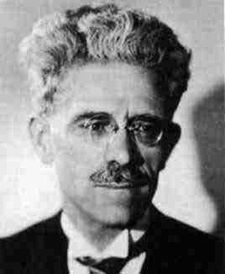
\includegraphics[width=.3\textwidth]{./fotos/Frechet.jpeg}\\[5pt]
{\small \bfseries Maurice Fréchet}
\end{bio}

Daremos en este capítulo ejemplos interesantes de espacios
métricos que aparecen de manera natural en muchas aplicaciones,
algunas de las cuales se verán más adelante.

\section{Definición y ejemplos}

\begin{definition}
  \label{defmet}Sea $X$ un conjunto. Una
  \textbf{métrica\index{metrica@métrica}} (o
  \textbf{distancia\index{distancia}}) en $X$ es una función
  $d\colon X\times X\rightarrow \mathbb{R}$ que tiene las siguientes tres
  propiedades:

  \begin{description}[font=\normalfont]
  \item[(M1)] $d(x,y)=0$ si y sólo si $x=y$.

  \item[(M2)] $d(x,y)=d(y,x)$  para cualesquiera $x,y\in X$.

  \item[(M3)] $d\left( x,z\right) \leq d(x,y)+d(y,z)$  para
    cualesquiera $x,y,z\in X$. A esta desigualdad se le llama la
    \textbf{desigualdad del triángulo\index{desigualdad!del triángulo}}.
  \end{description}

  Un \textbf{espacio métrico\index{espacio!metrico@métrico}} es un
  conjunto $X$ provisto de una métrica $d$. Lo denotaremos por
  $(X,d)$, o simplemente por $X$ cuando no haga falta especificar
  quién es su métrica.
\end{definition}

Veamos que la distancia entre dos puntos nunca es negativa.

\begin{proposition}
  $d(x,y)\geq 0$ para cualesquiera $x,y\in X$.
\end{proposition}

\begin{proof}
  De las propiedades (M1), (M3) y (M2) respectivamente se sigue que
  \begin{equation*}
    0=d(x,x)\leq d(x,y)+d(y,x)=2d(x,y).
  \end{equation*}
  En consecuencia, $d(x,y)\geq 0$ para todos $x,y\in X$.
\end{proof}

Los siguientes dos ejemplos de espacios métricos son bien
conocidos.

\begin{example}
  \label{R}El conjunto $\mathbb{R}$ de los números reales con la
  distancia usual
  \begin{equation*}
    d(x,y):=\left\vert x-y\right\vert =
    \begin{cases}
      x-y & \text{si $x\geq y$}, \\ 
      y-x & \text{si $x\leq y$},
    \end{cases}
  \end{equation*}
  es un espacio métrico.
\end{example}

\begin{example}
  \label{R2}El espacio euclidiano $\mathbb{R}^{n}$ con la distancia
  usual
  \begin{equation*}
    d_{2}(x,y):=\sqrt{(x_{1}-y_{1})^{2}+\cdots +(x_{n}-y_{n})^{2}},
  \end{equation*}
  donde $x=(x_{1},\dots,x_{n})$, $y=(y_{1},\dots,y_{n})\in
  \mathbb{R}^{n}$, es un espacio métrico.
\end{example}

La demostración de estas afirmaciones se propone como ejercicio
[Ejercicio~\ref{ejR}].

Podemos darle a $\mathbb{R}^{n}$ otras métricas interesantes, por
ejemplo las siguientes dos.

\begin{example}
  \label{R1}La función
  \begin{equation*}
    d_{1}(x,y):=\left\vert x_{1}-y_{1}\right\vert +\cdots +\left\vert
      x_{n}-y_{n}\right\vert ,
  \end{equation*}
  $x=(x_{1},\dots,x_{n})$, $y=(y_{1},\dots,y_{n})\in \mathbb{R}^{n}$, es
  una métrica para el espacio euclidiano $\mathbb{R}^{n}$.
\end{example}

\begin{proof}
  Las propiedades (M1) y (M2) son inmediatas y la propiedad (M3) se
  sigue de la desigualdad del triángulo en $\mathbb{R}$ que afirma
  que, para cada $i=1,\dots,n$,
  \begin{equation*}
    \left\vert x_{i}-z_{i}\right\vert \leq \left\vert x_{i}-y_{i}\right\vert
    +\left\vert y_{i}-z_{i}\right\vert .
  \end{equation*}
  Sumando ambos lados de estas desigualdades para $i=1,\dots,n$
  obtenemos
  \begin{equation*}
    d_{1}(x,z)\leq d_{1}(x,y)+d_{1}(y,z).
  \end{equation*}
  En consecuencia, $d_{1}$ es una métrica.
\end{proof}

\begin{example}
  \label{Rinf}La función
  \begin{equation*}
    d_{\infty }(x,y):=\max \left\{ \left\vert x_{1}-y_{1}\right\vert ,\ldots
      ,\left\vert x_{n}-y_{n}\right\vert \right\} ,
  \end{equation*}
  $x=(x_{1},\dots,x_{n})$, $y=(y_{1},\dots,y_{n})\in \mathbb{R}^{n}$, es
  una métrica para el espacio euclidiano $\mathbb{R}^{n}$.
\end{example}

La demostración es sencilla y se propone como ejercicio [Ejercicio
\ref{ejRinf}].

Introduciremos ahora métricas análogas en espacios de
sucesiones $(x_{k})$ de números reales.

\begin{example}
  \label{l-inf}Sea $\ell_{\infty }$ el conjunto de todas las
  sucesiones acotadas de números reales, es decir, de las
  sucesiones $\overline{x}=(x_{k})$ para las cuales existe $c\in
  \mathbb{R}$ (que depende de $\overline{x}$) tal que $\left\vert
    x_{k}\right\vert <c$ para todo $k\in \mathbb{N}$. Definimos
  \begin{equation*}
    d_{\infty }(\overline{x},\overline{y}):=\underset{k\geq 1}{\sup }\left\vert
      x_{k}-y_{k}\right\vert ,\text{\qquad }\overline{x}=(x_{k}),\text{ }\overline{y}=(y_{k})\in \ell_{\infty }.
  \end{equation*}
  Entonces $d_{\infty }$ toma valores en $\mathbb{R}$ y es una
  métrica en $\ell_{\infty }$.
\end{example}

\begin{proof}
  Sean $\overline{x}=(x_{k})$, $\overline{y}=(y_{k})$ sucesiones
  acotadas, y sean $c_{1},c_{2}\in \mathbb{R}$ tales que $\left\vert
    x_{k}\right\vert <c_{1}$ y $\left\vert y_{k}\right\vert <c_{2}$
  para todo $k\in \mathbb{N}$. De la desigualdad del triángulo
  para números reales se sigue que
  \begin{equation*}
    \left\vert x_{k}-y_{k}\right\vert \leq \left\vert x_{k}\right\vert
    +\left\vert y_{k}\right\vert \leq c_{1}+c_{2}\text{\qquad }\forall k\in 
    \mathbb{N},
  \end{equation*}
  {\abovedisplayskip=6pt 
  \belowdisplayskip=7pt 
  es decir, la sucesión $(x_{k}-y_{k})$ está acotada y, por
  tanto,
  \begin{equation*}
    d_{\infty }(\overline{x},\overline{y})=\underset{k\geq 1}{\sup }\left\vert
      x_{k}-y_{k}\right\vert \in \mathbb{R}.
  \end{equation*}
  Es inmediato comprobar que $d_{\infty }$ satisface las propiedades
  (M1) y (M2). Aplicando nuevamente desigualdad del triángulo para
  números reales obtenemos que, si
  $\overline{x},\overline{y},\overline{z}\in \ell_{\infty }$,
  entonces
  \begin{equation*}
    \left\vert x_{k}-y_{k}\right\vert \leq \left\vert x_{k}-z_{k}\right\vert
    +\left\vert z_{k}-y_{k}\right\vert \leq d_{\infty }(\overline{x},\overline{z})+d_{\infty }(\overline{z},\overline{y})\text{\qquad }\forall k\in \mathbb{N}.
  \end{equation*}
  En consecuencia,
  \begin{equation*}
    d_{\infty }(\overline{x},\overline{y})\leq d_{\infty }(\overline{x},\overline{z})+d_{\infty }(\overline{z},\overline{y})\text{\qquad }\forall 
    \overline{x},\overline{y},\overline{z}\in \ell_{\infty },
  \end{equation*}
  es decir, $d_{\infty }$ satisface (M3).}
\end{proof}

{\abovedisplayskip=8pt 
  \belowdisplayskip=7pt 
En los siguientes ejemplos requeriremos la noción de convergencia
de una serie. Recordemos que una serie de números reales
\begin{equation*}
  \sum_{k=1}^{\infty }x_{k}
\end{equation*}
converge, si la sucesión $(s_{n})$ de sumas finitas
\begin{equation*}
  s_{n}:=\sum_{k=1}^{n}x_{k}
\end{equation*}
converge. En tal caso, se denota
\begin{equation*}
  \sum_{k=1}^{\infty }x_{k}:=\lim_{n\rightarrow \infty }s_{n}.
\end{equation*}
Si $x_{k}\geq 0$ para todo $k\in \mathbb{N}$, entonces la sucesión
$(s_{n})$ es creciente. En ese caso, la serie converge si y sólo
si la sucesión $(s_{n})$ está acotada y, si eso ocurre, se
tiene que
\begin{equation*}
  \sum_{k=1}^{\infty }x_{k}=\lim_{n\rightarrow \infty }s_{n}=\sup_{n\geq
    1}s_{n}.
\end{equation*}

\begin{example}
  \label{l-1}Sea $\ell_{1}$ el conjunto de las sucesiones $(x_{k})$
  de números reales tales que la serie
  \begin{equation*}
    \sum_{k=1}^{\infty }\left\vert x_{k}\right\vert
  \end{equation*}
  converge, y sea
  \begin{equation*}
    d_{1}(\overline{x},\overline{y}):=\sum_{k=1}^{\infty }\left\vert
      x_{k}-y_{k}\right\vert ,\text{\qquad }\overline{x}=(x_{k}),\text{ }\overline{y}=(y_{k})\in \ell_{1}.
  \end{equation*}
  Entonces $d_{1}$ toma valores en $\mathbb{R}$ y es una métrica
  en $\ell_{1}$.
\end{example}

\begin{proof}
  De la desigualdad del triángulo para números reales,
  \begin{equation*}
    \left\vert x_{k}-y_{k}\right\vert \leq \left\vert x_{k}\right\vert
    +\left\vert y_{k}\right\vert,
  \end{equation*}
  se sigue que
  \begin{align*}
    \sum_{k=1}^{n}\left\vert x_{k}-y_{k}\right\vert &\leq
    \sum_{k=1}^{n}\left\vert x_{k}\right\vert +\sum_{k=1}^{n}\left\vert
      y_{k}\right\vert \\
    &\leq \sum_{k=1}^{\infty }\left\vert x_{k}\right\vert +\sum_{k=1}^{\infty
    }\left\vert y_{k}\right\vert .
  \end{align*}
  Por consiguiente, si $(x_{k}),(y_{k})\in \ell_{1}$, la serie
  $\sum_{k=1}^{\infty }\left\vert x_{k}-y_{k}\right\vert $ converge y
  se cumple que
  \begin{equation}
    \sum_{k=1}^{\infty }\left\vert x_{k}-y_{k}\right\vert \leq
    \sum_{k=1}^{\infty }\left\vert x_{k}\right\vert +\sum_{k=1}^{\infty
    }\left\vert y_{k}\right\vert .  \label{l1}
  \end{equation}
  Es fácil comprobar que $d_{1}$ satisface (M1) y (M2). La
  propiedad (M3) se sigue de la desigualdad (\ref{l1}) reemplazando
  $x_{k}$ por $x_{k}-z_{k}$ y $y_{k}$ por $y_{k}-z_{k}$, es decir,
  \begin{equation*}
    d_{1}(\overline{x},\overline{y})=\sum_{k=1}^{\infty }\left\vert
      x_{k}-y_{k}\right\vert \leq \sum_{k=1}^{\infty }\left\vert
      x_{k}-z_{k}\right\vert +\sum_{k=1}^{\infty }\left\vert
      z_{k}-y_{k}\right\vert =d_{1}(\overline{x},\overline{z})+d_{1}(\overline{z},\overline{y}),
  \end{equation*}
  para cualesquiera $\overline{x},\overline{y},\overline{z}\in \ell
 _{1}$.
\end{proof}}


\section{Espacios normados}

Nota que todos los ejemplos anteriores, además de la estructura
geométrica dada por la distancia, poseen una estructura
algebraica: la de espacio vectorial. Las métricas más
interesantes en un espacio vectorial son las inducidas por una norma.

\begin{definition}
  \label{defnor}Sea $V$ un espacio vectorial sobre $\mathbb{R}$. Una
  \textbf{norma}\index{norma} en $V$ es una función $\left\Vert
    \cdot \right\Vert \colon V\rightarrow \mathbb{R}$ que tiene las
  siguientes propiedades:

  \begin{description}[font=\normalfont]
  \item[(N1)] $\left\Vert v\right\Vert =0$ si y sólo si $v=0$,

  \item[(N2)] $\left\Vert \lambda v\right\Vert =\left\vert \lambda
    \right\vert \left\Vert v\right\Vert $ para cualesquiera $v\in
    V$, $\lambda \in \mathbb{R}$,

  \item[(N3)] $\left\Vert v+w\right\Vert \leq \left\Vert v\right\Vert
    +\left\Vert w\right\Vert $ para cualesquiera $v,w\in V$.
  \end{description}

  Un \textbf{espacio normado\index{espacio!normado}} es un espacio
  vectorial $V$ provisto de una norma $\left\Vert \cdot \right\Vert
  $. Lo denotaremos por $(V,\left\Vert \cdot \right\Vert )$, o
  simplemente por $V$ cuando no haga falta especificar quién es su
  norma.
\end{definition}

\begin{proposition}
  \label{evmet}Todo espacio normado $(V,\left\Vert \cdot \right\Vert
  )$ es un espacio métrico con la métrica dada por
  \begin{equation*}
    d(v,w):=\left\Vert v-w\right\Vert .
  \end{equation*}
  Esta métrica se llama la \textbf{métrica
    inducida\index{metrica@métrica!inducida por una norma}} por la norma\
  $\left\Vert \cdot \right\Vert $.
\end{proposition}

La demostración es sencilla y se propone como ejercicio [Ejercicio
\ref{ejevmet}].

Todas las métricas consideradas en los ejemplos anteriores
están inducidas por una norma. Veamos otros ejemplos.

Dado $x\in \mathbb{R}^{n}$ definimos
\index{norma!norma p@$\left\Vert \cdot \right\Vert_{p}$}
\begin{equation}
  \left. 
    \begin{aligned}
      &\left\Vert x\right\Vert_{p}:=\biggl( \sum_{k=1}^{n}\left\vert
          x_{k}\right\vert^{p}\biggr)^{\frac{1}{p}}\text{\qquad si }p\in [1,\infty ), \\ 
      &\left\Vert x\right\Vert_{\infty }:=\max_{1\leq k\leq n}\left\vert
        x_{k}\right\vert .
    \end{aligned}
  \right.  \label{normRn}
\end{equation}
Es sencillo comprobar que $\left\Vert \cdot \right\Vert_{p}$ cumple
las propiedades (N1) y (N2). Para probar que cumple la propiedad
(N3) requerimos unas desigualdades que demostraremos a
continuación.

\begin{lemma}[Desigualdad de Young]
  \label{young}Sean $p,q\in (1,\infty )$ tales que
  $\frac{1}{p}+\frac{1}{q}=1$. Entonces, para cualquier par de
  números reales $a,b\geq 0$ se cumple que\index{desigualdad!de Young}
  \begin{equation*}
    ab\leq 
    \tfrac{1}{p}a^{p}+\tfrac{1}{q}b^{q}.
  \end{equation*}
\end{lemma}

\begin{proof}
  Si $a=0$ o $b=0$ la desigualdad es obvia, de modo que podemos
  suponer que $ab>0$. La función exponencial es una función
  convexa, es decir, para cualesquiera $x_{0},x_{1}\in \mathbb{R}$ y
  $t\in [0,1]$ se cumple que
  \begin{equation*}
    (1-t)e^{x_{0}}+te^{x_{1}}\geq e^{\left[ (1-t)x_{0}+tx_{1}\right] }.
  \end{equation*}
  \begin{figure}[H]
    \centering
    \begin{tikzpicture}[domain=-2:2.6, xscale=2,yscale=1.5]
  \pgfmathsetmacro{\xo}{0.5}
  \pgfmathsetmacro{\yo}{.2*exp(\xo)}
  \pgfmathsetmacro{\xi}{2.2}
  \pgfmathsetmacro{\yi}{.2*exp(\xi)}
  \pgfmathsetmacro{\xt}{1.4}
  \pgfmathsetmacro{\yt}{.2*exp(\xt)}
  \pgfmathsetmacro{\yl}{(\yi-\yo)/(\xi-\xo)*(\xt-\xo)+\yo}

  \coordinate (p0) at (\xo,\yo);
  \coordinate (p1) at (\xi,\yi);
  \coordinate (p2) at (\xt,\yt);

  \draw[-latex'] (-2,0)--(2.85,0);
  \draw[-latex'] (0,-.2)--(0,{.2*exp(2.7)});
  \draw[very thick] plot(\x,{.2*exp(\x)});
  \draw[thin] (p0)--(p1);
  \draw[only marks,mark=*, mark size=1pt, ScalePlotMarksOff] plot
  coordinates {(p0) (p1)};
  \draw (2.65,{.2*exp(2.5)}) node[right] {$y=e^x$};

  \draw[thin,densely dotted] (\xo,0)--(p0);
  \draw[thin,densely dotted] (\xi,0)--(p1);
%  \draw[thin,densely dotted] (p0)--(0,\yo);
%  \draw[thin,densely dotted] (p1)--(0,\yi);

  \draw[thin,densely dotted] (\xt,0)--(\xt,\yl)--(0,\yl);
  \draw[thin,densely dotted] (0,\yt)--(\xt,\yt);
  
  \draw (\xo,0) node[below] {$x_0$};
  \draw (\xt,0) node[below] {$(1-t)x_0+tx_1$};
  \draw (\xi,0) node[below] {$x_1$};

  \draw (0,\yl) node[left] {$(1-t)e^{x_0}+te^{x_1}$};
  \draw (0,\yt) node[left] {$e^{(1-t)x_0+tx_1}$};


\end{tikzpicture}

    % \caption{}\label{fig:2.1}
  \end{figure}
  \noindent
  Tomando $x_{0}=\ln a^{p}$, $x_{1}=\ln b^{q}$ y $t=\frac{1}{q}$
  obtenemos
  \begin{equation*}
    \tfrac{1}{p}a^{p}+\tfrac{1}{q}b^{q}\geq e^{(\frac{1}{p}\ln a^{p}+\frac{1}{q}\ln b^{q})}=ab.
  \end{equation*}
  Esta es la desigualdad deseada.
\end{proof}

Aplicaremos la desigualdad de Young\footnote{William Henry Young
  (1863-1942) nació en Londres, Inglaterra. Estudió
  matemáticas en Cambridge y fue profesor en diversas
  universidades europeas. Publicó esta desigualdad en 1912.} para
demostrar la desigualdad de Hölder\footnote{Otto Ludwig Hölder
  (1859-1937) nació en Stuttgart, Alemania. Estudió en las
  universidades de Stuttgart y Berlín, donde fue estudiante de
  Kronecker, Weierstrass y Kummer. Obtuvo el doctorado en la
  Universidad de Tübingen en 1882. Descubrió la desigualdad
  que lleva su nombre en 1884, cuando trabajaba en la convergencia de
  series de Fourier.}.

\begin{multicols}{2}
\begin{bio}
\centering

\includegraphics[width=.33\textwidth]{./fotos/calcasdos/Young_2.pdf}\\[5pt]
 {\small\bfseries William Henry Young}
\end{bio}

\begin{bio}
  \centering
  
\includegraphics[width=.36\textwidth]{./fotos/calcasdos/Hoelder_Otto.pdf}\\[5pt]
  {\small\bfseries Otto Hölder}
\end{bio}
\end{multicols}

\begin{proposition}[Desigualdad de Hölder en $\mathbb{R}^{n}$]
  \label{Rholder}Sean $p,q\in (1,\infty )$ tales que\break
  $\frac{1}{p}+\frac{1}{q}=1$. Entonces, para cualesquiera
  $x=(x_{1},\dots,x_{n})$, $y=(y_{1},\dots,y_{n})\in \mathbb{R}^{n}$ se
  cumple que\index{desigualdad!de Hölder!en $\mathbb{R}^{n}$}
  \begin{equation*}
    \sum_{k=1}^{n}\left\vert x_{k}y_{k}\right\vert \leq \biggl(
      \sum_{k=1}^{n}\left\vert x_{k}\right\vert^{p}\biggr)^{\frac{1}{p}}\biggl( \sum_{k=1}^{n}\left\vert y_{k}\right\vert^{q}\biggr)^{\frac{1}{q}},
  \end{equation*}
  es decir,
  \begin{equation*}
    \left\Vert xy\right\Vert_{1}\leq \left\Vert x\right\Vert_{p}\left\Vert
      y\right\Vert_{q}
  \end{equation*}
  donde $xy:=(x_{1}y_{1},\dots,x_{n}y_{n})$.
\end{proposition}

\begin{proof}
  La afirmación es trivial si $x=0$ o si $y=0$. Supongamos pues
  que ambos son distintos de cero. Aplicando la desigualdad de Young a
  \begin{equation*}
    a_{k}:=\frac{\left\vert x_{k}\right\vert }{\left\Vert x\right\Vert_{p}}\text{\qquad y\qquad }b_{k}:=\frac{\left\vert y_{k}\right\vert }{\left\Vert
        y\right\Vert_{q}}
  \end{equation*}
  obtenemos
  \begin{equation*}
    \frac{\left\vert x_{k}y_{k}\right\vert }{\left\Vert x\right\Vert
     _{p}\left\Vert y\right\Vert_{q}}\leq \frac{\left\vert x_{k}\right\vert^{p}}{p\left\Vert x\right\Vert_{p}^{p}}+\frac{\left\vert y_{k}\right\vert^{q}}{q\left\Vert y\right\Vert_{q}^{q}}.
  \end{equation*}
  Sumando todas estas desigualdades para $k=1,\dots,n$, concluimos que
  \begin{align*}
    \frac{1}{\left\Vert x\right\Vert_{p}\left\Vert y\right\Vert_{q}}\biggl(
      \sum_{k=1}^{n}\left\vert x_{k}y_{k}\right\vert \biggr) &\leq \frac{1}{p\left\Vert x\right\Vert_{p}^{p}}\biggl( \sum_{k=1}^{n}\left\vert
        x_{k}\right\vert^{p}\biggr) +\frac{1}{q\left\Vert y\right\Vert_{q}^{q}}\biggl( \sum_{k=1}^{n}\left\vert y_{k}\right\vert^{q}\biggr) \\
    &=\frac{1}{p}+\frac{1}{q}=1.
  \end{align*}
  Multiplicando ambos lados de la desigualdad anterior por $\left\Vert
    x\right\Vert_{p}\left\Vert y\right\Vert_{q}$ obtenemos la
  desigualdad deseada.
\end{proof}

Estamos listos para demostrar el siguiente resultado.

\begin{proposition}
  \label{Rp}Para cada $p\in [1,\infty ]$, la función
  $\left\Vert \cdot \right\Vert_{p}$ definida en
  \emph{(\ref{normRn})} es una norma en $\mathbb{R}^{n}$.
\end{proposition} {\abovedisplayskip=7pt
  \belowdisplayskip=8pt \begin{proof} Es sencillo ver que
    $\left\Vert \cdot \right\Vert_{p}$ cumple las propiedades (N1) y
    (N2). Demostremos la propiedad (N3), es decir, que para todo
    $p\in [1,\infty ]$ se cumple que \begin{equation} \left\Vert
        x+y\right\Vert_{p}\leq \left\Vert x\right\Vert_{p}+\left\Vert
        y\right\Vert_{p}\text{\qquad }\forall x,y\in
      \mathbb{R}^{n}.  \label{minkRp} \end{equation} Para $p=\infty $
    esta desigualdad es consequencia inmediata de la desigualdad del
    triángulo para números reales [Ejercicio~\ref{ejRinf}]. El caso
    $p=1$ se probó en el Ejemplo~\ref{R1}.

  Tomemos ahora $p\in (1,\infty )$. La afirmación es trivial si
  $x=0$. Supongamos pues que $x\neq 0$ y apliquemos la desigualdad de
  Hölder a $x$ y $((\left\vert x_{1}\right\vert +\left\vert
    y_{1}\right\vert )^{p-1},\ldots ,(\left\vert x_{n}\right\vert
  +\left\vert y_{n}\right\vert )^{p-1})$. Definiendo
  $q:=\frac{p}{p-1}$ obtenemos
  \begin{equation*}
    \sum_{k=1}^{n}\left\vert x_{k}\right\vert (\left\vert
      x_{k}\right\vert +\left\vert y_{k}\right\vert )^{p-1}\leq \left\Vert
      x\right\Vert_{p}\biggl( \sum_{k=1}^{n}(\left\vert x_{k}\right\vert
      +\left\vert y_{k}\right\vert )^{p}\biggr)^{\frac{1}{q}},
  \end{equation*}
  Análogamente,
  \begin{equation*}
    \sum_{k=1}^{n}\left\vert y_{k}\right\vert (\left\vert
      x_{k}\right\vert +\left\vert y_{k}\right\vert )^{p-1}\leq \left\Vert
      y\right\Vert_{p}\biggl( \sum_{k=1}^{n}(\left\vert x_{k}\right\vert
      +\left\vert y_{k}\right\vert )^{p}\biggr)^{\frac{1}{q}}.
  \end{equation*}
  Sumando las dos desigualdades anteriores obtenemos
  \begin{equation*}
    \sum_{k=1}^{n}(\left\vert x_{k}\right\vert +\left\vert
      y_{k}\right\vert )^{p}\leq \left( \left\Vert x\right\Vert_{p}+\left\Vert
        y\right\Vert_{p}\right) \biggl( \sum_{k=1}^{n}(\left\vert
        x_{k}\right\vert +\left\vert y_{k}\right\vert )^{p}\biggr)^{\frac{1}{q}}.
  \end{equation*}
  Dividiendo ambos lados de esta desigualdad entre
  \begin{equation*}
    \biggl( \sum_{k=1}^{n}(\left\vert x_{k}\right\vert +\left\vert
        y_{k}\right\vert )^{p}\biggr)^{\frac{1}{q}}
  \end{equation*}
  y usando la desigualdad del triángulo para números reales
  $\left\vert x_{k}+y_{k}\right\vert \leq \left\vert x_{k}\right\vert
  +\left\vert y_{k}\right\vert $, concluimos que
  \begin{equation*}
    \left\Vert x+y\right\Vert_{p}=\biggl( \sum_{k=1}^{n}\left\vert
        x_{k}+y_{k}\right\vert^{p}\biggr)^{\frac{1}{p}}\leq \left(
      \sum_{k=1}^{n}(\left\vert x_{k}\right\vert +\left\vert
        y_{k}\right\vert )^{p}\right)^{\frac{1}{p}}\leq \left\Vert x\right\Vert
   _{p}+\left\Vert y\right\Vert_{p}.
  \end{equation*}
  Ésta es la desigualdad deseada.
\end{proof}}

\begin{notation}
  Con el fin de distinguir cuál de todas estas normas estamos
  considerando, usaremos la notación\index{espacio!Rn@$\mathbb{R}_{p}^{n}$}
  \begin{equation}
    \mathbb{R}_{p}^{n}:=(\mathbb{R}^{n},\left\Vert \cdot \right\Vert
   _{p}),\qquad p\in [1,\infty ],  \label{Rnp}
  \end{equation}
  para designar al espacio $\mathbb{R}^{n}$ con la norma $\left\Vert
    \cdot \right\Vert_{p}$. Escribiremos simplemente $\mathbb{R}^{n}$
  \index{espacio!Rn@$\mathbb{R}^{n}$}en vez de
  $\mathbb{R}_{2}^{n}$ para designar a $\mathbb{R}^{n}$ con la norma
  usual, a la que denotaremos simplemente por
  \begin{equation}
    \left\Vert x\right\Vert :=\sqrt{x_{1}^{2}+\cdots +x_{n}^{2}}.  \label{normausual}
  \end{equation}
\end{notation}

Nota que las métricas $d_{1},d_{2}$ y $d_{\infty }$ consideradas
en los Ejemplos~\ref{R2} al~\ref{Rinf} son las inducidas por las
normas $\left\Vert \cdot \right\Vert_{1}$, $\left\Vert \cdot
\right\Vert $ y $\left\Vert \cdot \right\Vert_{\infty }$,
respectivamente.

Consideremos ahora espacios de sucesiones. Las sucesiones de
números reales se pueden sumar y multiplicar por escalares
término a término, es decir, si $\overline{x}=(x_{k})$ y
$\overline{y}=(y_{k})$ son sucesiones de números reales y $\lambda
\in \mathbb{R}$, se definen
\begin{equation*}
  \overline{x}+\overline{y}:=(x_{k}+y_{k})\text{ \qquad y\qquad }\lambda 
  \overline{x}:=(\lambda x_{k}).
\end{equation*}
Con estas operaciones el conjunto de todas las sucesiones de
números reales es un espacio vectorial. Para espacios de
sucesiones adecuados podemos definir normas análogas a las
definidas para $\mathbb{R}^{n}$.

\begin{proposition}
  \label{l-p}

  \begin{enumerate}
  \item[(a)] Si $p\in [1,\infty )$, el conjunto $\ell_{p}$
    \index{espacio!l subp@$\ell_{p}$}de todas las sucesiones
    de números reales $(x_{k})$ tales que la serie
    \begin{equation*}
      \sum_{k=1}^{\infty }\left\vert x_{k}\right\vert^{p}
    \end{equation*}
    converge es un espacio vectorial y
\index{norma!norma p@$\left\Vert \cdot \right\Vert_{p}$}
    \begin{equation}
      \left\Vert (x_{k})\right\Vert_{p}:=\biggl( \sum_{k=1}^{\infty
        }\left\vert x_{k}\right\vert^{p}\biggr)^{\frac{1}{p}}  \label{normlp}
    \end{equation}
    es una norma en $\ell_{p}$.

  \item[(b)] El conjunto $\ell_{\infty }$ de todas las sucesiones
    acotadas de números reales es un espacio vectorial y
    \begin{equation}
      \left\Vert (x_{k})\right\Vert_{\infty }:=\underset{k\geq 1}{\sup }\left\vert x_{k}\right\vert  \label{normlinf}
    \end{equation}
    es una norma en $\ell_{\infty }$.
  \end{enumerate}
\end{proposition}

\begin{proof}
  Es sencillo ver que $\lambda \overline{x}\in \ell_{p}$ para
  cualesquiera $\overline{x}\in \ell_{p}$, $\lambda \in \mathbb{R}$,
  y que $\left\Vert \cdot \right\Vert_{p}$ cumple las propiedades
  (N1) y (N2) [Ejercicio~\ref{ejlp}]. Probaremos a continuación
  que $\overline{x}+\overline{y}\in \ell_{p}$ si
  $\overline{x},\overline{y}\in \ell_{p}$ y que $\left\Vert \cdot
  \right\Vert_{p}$ cumple la propiedad (N3).

  \emph{(a):}  Si $p\in [1,\infty )$ y $(x_{k}),(y_{k})\in
  \ell_{p}$, como la norma $\left\Vert \cdot \right\Vert_{p}$ en
  $\mathbb{R}^{n}$ satisface la propiedad (N3), se tiene que
  \begin{equation*}
    \biggl( \sum_{k=1}^{n}\left\vert x_{k}+y_{k}\right\vert^{p}\biggr)^{\frac{1}{p}}\leq \biggl( \sum_{k=1}^{n}\left\vert x_{k}\right\vert
     ^{p}\biggr)^{\frac{1}{p}}+\biggl( \sum_{k=1}^{n}\left\vert
        y_{k}\right\vert^{p}\biggr)^{\frac{1}{p}}\leq \left\Vert
      (x_{k})\right\Vert_{p}+\left\Vert (y_{k})\right\Vert_{p}
  \end{equation*}
  para todo $n\in \mathbb{N}$. En consecuencia, la serie
  $\sum_{k=1}^{\infty }\left\vert x_{k}+y_{k}\right\vert^{p}$
  converge y se cumple que
  \begin{equation*}
    \left\Vert (x_{k}+y_{k})\right\Vert_{p}=\biggl( \sum_{k=1}^{\infty
      }\left\vert x_{k}+y_{k}\right\vert^{p}\biggr)^{\frac{1}{p}}\leq \left\Vert
      (x_{k})\right\Vert_{p}+\left\Vert (y_{k})\right\Vert_{p}.
  \end{equation*}

  \emph{(b):}  El caso $p=\infty $ se probó en el Ejemplo~\ref{l-inf}.
\end{proof}

Si $p\in [1,\infty )$ la desigualdad (N3) en $\ell_{p}\ $se
llama la \textbf{desigualdad de Minkowski para
  series}\index{desigualdad!de Minkowski!para series}. Nota que las
métricas $d_{1}$ y $d_{\infty }$ consideradas en los Ejemplos
\ref{l-1} y~\ref{l-inf} son las inducidas por las normas $\left\Vert
  \cdot \right\Vert_{1}$ y $\left\Vert \cdot \right\Vert_{\infty }$
que acabamos de definir.

No cualquier métrica en un espacio vectorial está inducida por
una norma. De hecho, a cualquier conjunto le podemos dar la
métrica siguiente.

\begin{example}
  \label{disc}Sea $X$ un conjunto arbitrario. La función
  \begin{equation*}
    d_{\disc}(x,y)=
      \begin{cases}
        0&\text{si $x=y$,} \\ 
        1&\text{si $x\neq y,$}
      \end{cases}
  \end{equation*}
  es una métrica en $X$, llamada la \textbf{métrica
    discreta\index{metrica@métrica!discreta@discreta $d_{\disc}$}}. El
  espacio $X_{\disc}:=(X,d_{\disc})$ se llama un \textbf{espacio
    discreto\index{espacio!discreto@discreto $X_{\disc}$}}.
\end{example}

Es sencillo comprobar que en un espacio vectorial no trivial ninguna
norma induce la métrica discreta [Ejercicio~\ref{ejdiscnoev}].

\section{Espacios de funciones}

\label{espfunc}Denotemos por $\mathcal{C}^{0}[a,b]$ al conjunto de
todas las funciones continuas $f\colon [a,b]\rightarrow \mathbb{R}$. La suma
de funciones y el producto de una función por un escalar,
definidos como
\begin{equation*}
  (f+g)(x):=f(x)+g(x),\text{\qquad }(\lambda f)(x):=\lambda f(x),\text{\qquad }f,g\in \mathcal{C}^{0}[a,b],\text{ }\lambda \in \mathbb{R},
\end{equation*}
le dan a $\mathcal{C}^{0}[a,b]$ la estructura de espacio vectorial. \
Dada $f\in \mathcal{C}^{0}[a,b]$
definimos\index{norma!norma p@$\left\Vert \cdot \right\Vert_{p}$}
\begin{equation}
    \begin{aligned}
      &\left\Vert f\right\Vert_{p}:=\biggl(\int_{a}^{b}\left\vert f(x)\right\vert
       ^{p}dx\biggr)^{\frac{1}{p}}\text{\qquad si }p\in [1,\infty ), \\ 
      &\left\Vert f\right\Vert_{\infty }:=\max \left\{\left\vert f(x)\right\vert :a\leq
      x\leq b\right\}.
    \end{aligned}\label{normfunc}
\end{equation}
Demostraremos a continuación que éstas son normas en
$\mathcal{C}^{0}[a,b]$. Empecemos observando lo siguiente.

\begin{lemma}
  \label{N1int}Sean $f\in \mathcal{C}^{0}[a,b]$ y $p\in [1,\infty ]$. Entonces, $\left\Vert f\right\Vert_{p}=0$ si y
  sólo si $f=0$.
\end{lemma}

\begin{proof}
  Para $p=\infty $ esta afirmación es consecuencia inmediata de la
  definición (\ref{normfunc}). Si $p\in [1,\infty )$, como
  $\left\vert f(x)\right\vert^{p}$ es una función continua y no
  negativa, se tiene que
  \begin{equation*}
    \left\Vert f\right\Vert_{p}^{p}=\int_{a}^{b}\left\vert f(x)\right\vert
   ^{p}dx=0\quad \Longleftrightarrow \quad \left\vert f(x)\right\vert^{p}=0\text{ }\forall x\in [a,b].
  \end{equation*}
  En consecuencia, $\left\Vert f\right\Vert_{p}=0$ si y sólo si
  $f=0$.
\end{proof}

Probaremos ahora la desigualdad de Hölder para integrales. Su
demostración es análoga a la correspondiente para
$\mathbb{R}^{n}$.

\begin{proposition}[Desigualdad de Hölder para integrales]
  \label{iholder}\index{desigualdad!de Hölder}Sean $p,q\in
  (1,\infty )$ tales que $\frac{1}{p}+\frac{1}{q}=1$. Entonces, para
  cualquier par de funciones continuas $f,g\colon [a,b]\rightarrow
  \mathbb{R}$ se cumple que
  \begin{equation*}
    \int_{a}^{b}\left\vert f(x)g(x)\right\vert dx\leq \biggl(
      \int_{a}^{b}\left\vert f(x)\right\vert^{p}dx\biggr)^{\frac{1}{p}}\biggl(
      \int_{a}^{b}\left\vert g(x)\right\vert^{q}dx\biggr)^{\frac{1}{q}},
  \end{equation*}
  es decir,
  \begin{equation*}
    \left\Vert fg\right\Vert_{1}\leq \left\Vert f\right\Vert_{p}\left\Vert
      g\right\Vert_{q}.
  \end{equation*}
\end{proposition}

\begin{proof}
  La afirmación es trivial si $f=0$ o si $g=0$. Supongamos pues
  que ambas funciones son distintas de cero. Para cada $x\in [a,b]$, definimos
  \begin{equation*}
    a_{x}:=\frac{\left\vert f(x)\right\vert }{\left\Vert f\right\Vert_{p}}\text{\qquad y\qquad }b_{x}:=\frac{\left\vert g(x)\right\vert }{\left\Vert
        g\right\Vert_{q}}.
  \end{equation*}
  Aplicando la desigualdad de Young (Lema~\ref{young}) a estos
  números obtenemos
  \begin{equation*}
    \frac{\left\vert f(x)g(x)\right\vert }{\left\Vert f\right\Vert
     _{p}\left\Vert g\right\Vert_{q}}\leq \frac{\left\vert f(x)\right\vert^{p}}{p\left\Vert f\right\Vert_{p}^{p}}+\frac{\left\vert g(x)\right\vert^{q}}{q\left\Vert g\right\Vert_{q}^{q}},
  \end{equation*}
  e integrando ambos lados de esta desigualdad concluimos que
  \begin{equation*}
    \frac{\int_{a}^{b}\left\vert f(x)g(x)\right\vert dx}{\left\Vert f\right\Vert
     _{p}\left\Vert g\right\Vert_{q}}\leq \frac{\int_{a}^{b}\left\vert
        f(x)\right\vert^{p}dx}{p\left\Vert f\right\Vert_{p}^{p}}+\frac{\int_{a}^{b}\left\vert g(x)\right\vert^{q}dx}{q\left\Vert g\right\Vert
     _{q}^{q}}=\frac{1}{p}+\frac{1}{q}=1\text{.}
  \end{equation*}
  Multiplicando ambos lados de esta desigualdad por $\left\Vert
    f\right\Vert_{p}\left\Vert g\right\Vert_{q}$ obtenemos la
  desigualdad deseada.
\end{proof}

Es fácil ver que también vale la desigualdad de Hölder
\begin{equation*}
  \left\Vert fg\right\Vert_{1}\leq \left\Vert f\right\Vert_{1}\left\Vert
    g\right\Vert_{\infty }
\end{equation*}
[Ejercicio~\ref{ejholder1inf}]. A partir de la desigualdad de Hölder se
obtiene la desigualdad de Minkowski\footnote{Hermann Minkowski (1864-1909) nació en Lituania, entonces parte del
  Imperio Ruso. Obtuvo el doctorado en 1885 en la Universidad Albertina de Königsberg. Fue profesor en la ETH de Zürich y en la Universidad de Göttingen, ciudad en la que murió.}.
\begin{bio}
\centering
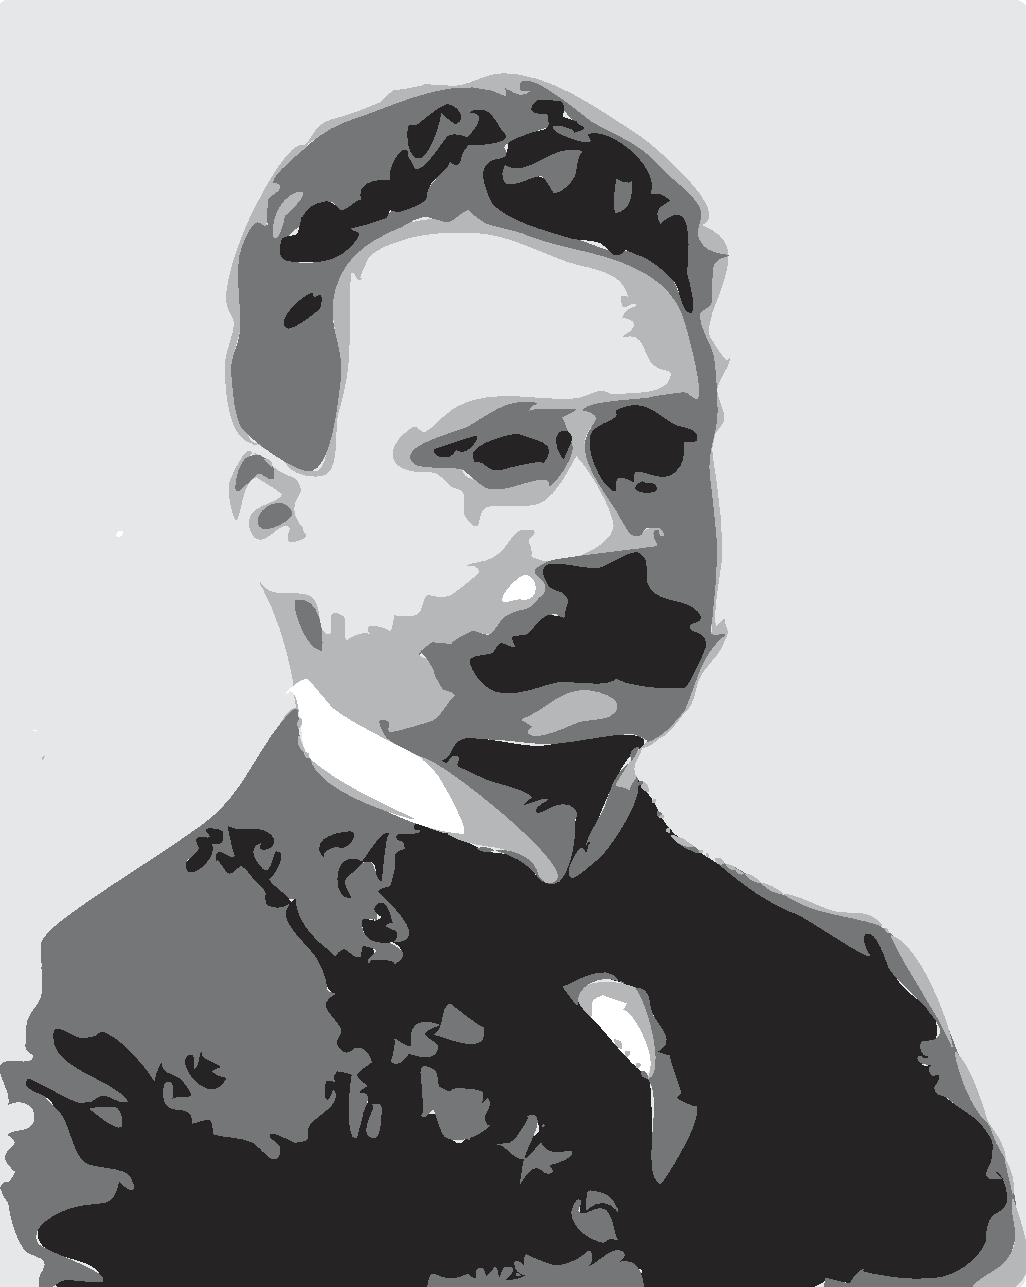
\includegraphics[width=.25\textwidth]{./fotos/calcasdos/minkowski.pdf}\\[5pt]
 {\small\bfseries Hermann Minkowski}
\end{bio}

\begin{proposition}[Desigualdad de Minkowski para integrales]
  \label{imink}\index{desigualdad!de Minkowski}Sea $p\in [1,\infty ]$. Entonces,
  \begin{equation*}
    \left\Vert f+g\right\Vert_{p}\leq \left\Vert f\right\Vert_{p}+\left\Vert
      g\right\Vert_{p}\text{\qquad }\forall f,g\in \mathcal{C}^{0}[a,b].
  \end{equation*}
\end{proposition}

\begin{proof}
  Los casos $p=1,\infty $ se proponen como ejercicio [Ejercicio~\ref{ejmink1inf}].

  Sea $p\in (1,\infty )$. Si $f=0$ la afirmación es
  evidente. Supongamos pues que $f\neq 0$. Sea
  $h(x)=(\left\vert f(x)\right\vert +\left\vert g(x)\right\vert
  )^{p-1}$.
  Aplicando la desigualdad de Hölder para integrales
  (Proposición~\ref{iholder}) a las funciones $f,h$, y $g,h$
  respectivamente, obtenemos
  \begin{align*}
    \int_{a}^{b}\left\vert f(x)\right\vert (\left\vert f(x)\right\vert
    +\left\vert g(x)\right\vert )^{p-1}dx &\leq \left\Vert f\right\Vert
   _{p}\biggl( \int_{a}^{b}(\left\vert f(x)\right\vert +\left\vert
        g(x)\right\vert )^{p}\,dx\biggr)^{\frac{1}{q}}, \\
    \int_{a}^{b}\left\vert g(x)\right\vert (\left\vert f(x)\right\vert
    +\left\vert g(x)\right\vert )^{p-1}dx &\leq \left\Vert g\right\Vert
   _{p}\biggl( \int_{a}^{b}(\left\vert f(x)\right\vert +\left\vert
        g(x)\right\vert )^{p}\,dx\biggr)^{\frac{1}{q}},
  \end{align*}
  y sumando estas desigualdades concluimos que
  \begin{equation*}
    \int_{a}^{b}(\left\vert f(x)\right\vert +\left\vert g(x)\right\vert
    )^{p}dx\leq \left( \left\Vert f\right\Vert_{p}+\left\Vert g\right\Vert
     _{p}\right) \biggl( \int_{a}^{b}(\left\vert f(x)\right\vert +\left\vert
        g(x)\right\vert )^{p}\,dx\biggr)^{\frac{1}{q}}.
  \end{equation*}
  Dividiendo ambos lados de esta desigualdad entre
  \begin{equation*}
    \biggl( \int_{a}^{b}(\left\vert f(x)\right\vert +\left\vert g(x)\right\vert
      )^{p}\,dx\biggr)^{\frac{1}{q}}
  \end{equation*}
  y usando la desigualdad del triángulo para números reales
  $\left\vert f(x)+g(x)\right\vert \leq \left\vert f(x)\right\vert
  +\left\vert g(x)\right\vert $ y la monotonía de la integral
  obtenemos
  \begin{align*}
    \left\Vert f+g\right\Vert_{p}&=\biggl( \int_{a}^{b}\left\vert
        f(x)+g(x)\right\vert^{p}dx\biggr)^{\frac{1}{p}}\\
&\leq \biggl(
      \int_{a}^{b}\left( \left\vert f(x)\right\vert +\left\vert g(x)\right\vert
      \right)^{p}dx\biggr)^{\frac{1}{p}}\leq \left\Vert f\right\Vert
   _{p}+\left\Vert g\right\Vert_{p},
  \end{align*}
  como afirma el enunciado.
\end{proof}

Ahora podemos concluir lo siguiente.

\begin{proposition}
  Para cada $p\in [1,\infty ]$ la función $\left\Vert \cdot
  \right\Vert_{p}$ definida en \emph{(\ref{normfunc})} es una norma
  en $\mathcal{C}^{0}[a,b]$.
\end{proposition}

\begin{proof}
  Las propiedades (N1) y (N3) se probaron en el Lema~\ref{N1int} y la
  Proposición~\ref{imink} respectivamente. La propiedad (N2) es
  consecuencia inmediata de la linealidad de la integral.
\end{proof}

\begin{notation}
  Con el fin de distinguir cuál de todas estas normas estamos
  considerando, usaremos la
  notación\index{espacio!C subp0ab@$\mathcal{C}_{p}^{0}[a,b]\vspaceindex$}
  \begin{equation*}
    \mathcal{C}_{p}^{0}[a,b]:=(\mathcal{C}^{0}[a,b],\left\Vert \cdot \right\Vert
   _{p}),\text{\qquad }p\in [1,\infty ],
  \end{equation*}
  para designar al espacio de las funciones continuas
  $f\colon [a,b]\rightarrow \mathbb{R}$ con la norma $\left\Vert \cdot
  \right\Vert_{p}$. Como veremos más adelante, la norma más
  adecuada en el espacio de funciones continuas $\mathcal{C}^{0}[a,b]$
  es la norma $\left\Vert \cdot \right\Vert_{\infty }$. Por ello,
  escribiremos
  simplemente\index{espacio!C ala0ab@$\mathcal{C}^{0}[a,b]$}
  \begin{equation*}
    \mathcal{C}^{0}[a,b]:=(\mathcal{C}^{0}[a,b],\left\Vert \cdot \right\Vert
   _{\infty }).
  \end{equation*}
\end{notation}

Observa que la distancia $\left\Vert f-g\right\Vert_{\infty }$ entre
dos funciones continuas$\ f$ y $g$ es pequeña si sus gráficas
están cerca la una de la otra, mientras que la distancia
$\left\Vert f-g\right\Vert_{1}$ es pequeña si el área de la
región delimitada por sus gráficas es pequeña. Así,
dos funciones continuas pueden estar muy cerca según la norma
$\left\Vert \cdot \right\Vert_{1}$ y a distancia arbitrariamente
grande según la norma $\left\Vert \cdot \right\Vert_{\infty }$,
como lo muestra el siguiente ejemplo.

\begin{example}
  \label{difnorm1inf}Sean $R>0$ y $f_{k}\colon [0,1]\rightarrow \mathbb{R}$
  la función dada por
  \begin{equation*}
    f_{k}(x)=
      \begin{cases}
        R(1-kx) & 
        \text{si $0\leq x\leq \frac{1}{k}$,} \\ 
        0 & \text{si $\frac{1}{k}\leq x\leq 1.$}
      \end{cases}
  \end{equation*}
  Entonces $\left\Vert f_{k}\right\Vert_{\infty }=R$ para toda $k\in
  \mathbb{N}$, mientras que $\left\Vert f_{k}\right\Vert
 _{1}=\frac{R}{2k}$.
  \begin{figure}[H]
    \centering
    \begin{tikzpicture}[domain=-.1:1.2,scale=2]
  \draw (-.05,0)--(1.1,0);
  \draw (0,-.05)--(0,1.1);
  \draw[very thick] (0,1)--(.25,0)--(1,0);
  \foreach \x in {0.25, 0.5, 0.75, 1}{
               \draw[thin] (\x,-0.05)--(\x,0);
               \draw[thin] (-.05,\x)--(0,\x);
};
\draw (.15,.6) node[right] {$y=f_4(x)$};
% \draw (0,-.05) node[below] {$0$};
% \draw (.25,-.05) node[below] {$\frac{1}{4}$};
% \draw (.5,-.05) node[below] {$\frac{1}{2}$};
% \draw (.75,-.05) node[below] {$\frac{3}{4}$};
% \draw (1,-.05) node[below] {$1$};
% \draw (-.05,0) node[left] {$0$};
% \draw (-.05,.25) node[left] {$\frac{1}{4}$};
% \draw (-.05,.5) node[left] {$\frac{1}{2}$};
% \draw (-.05,.75) node[left] {$\frac{3}{4}$};
% \draw (-.05,1) node[left] {$1$};
\end{tikzpicture}
\qquad\qquad
    \begin{tikzpicture}[domain=-.1:1.2,scale=2]
  \draw (-.05,0)--(1.1,0);
  \draw (0,-.05)--(0,1.1);
  \draw[very thick] (0,1)--(.125,0)--(1,0);
  \foreach \x in {0.25, 0.5, 0.75, 1}{
               \draw[thin] (\x,-0.05)--(\x,0);
               \draw[thin] (-.05,\x)--(0,\x);
};
\draw (.1,.6) node[right] {$y=f_8(x)$};
% \draw (0,-.05) node[below] {$0$};
% \draw (.25,-.05) node[below] {$\frac{1}{4}$};
% \draw (.5,-.05) node[below] {$\frac{1}{2}$};
% \draw (.75,-.05) node[below] {$\frac{3}{4}$};
% \draw (1,-.05) node[below] {$1$};
% \draw (-.05,0) node[left] {$0$};
% \draw (-.05,.25) node[left] {$\frac{1}{4}$};
% \draw (-.05,.5) node[left] {$\frac{1}{2}$};
% \draw (-.05,.75) node[left] {$\frac{3}{4}$};
% \draw (-.05,1) node[left] {$1$};
\end{tikzpicture}

    % \caption{}
  \end{figure}
  \noindent
  Es decir, según la norma $\left\Vert \cdot \right\Vert_{\infty
  }$ todas las funciones $f_{k}$ distan exactamente $R$ de la
  función constante igual a $0$, mientras que, según la norma
  $\left\Vert \cdot \right\Vert_{1}$, dichas funciones se acercan
  cada vez más a la función $0$ conforme $k$ crece.
\end{example}

Las normas definidas en esta sección satisfacen las siguientes
relaciones.

\begin{proposition}
  \label{compinorm}Para toda $f\in \mathcal{C}^{0}[a,b]$ se cumple que
  \begin{align*}
    \left\Vert f\right\Vert_{s} &\leq (b-a)^{\frac{r-s}{rs}}\left\Vert
      f\right\Vert_{r}\text{\qquad }\forall 1\leq s<r<\infty , \\
    \left\Vert f\right\Vert_{s} &\leq (b-a)^{\frac{1}{s}}\left\Vert
      f\right\Vert_{\infty }\text{\qquad }\forall 1\leq s<\infty .
  \end{align*}
\end{proposition}

\begin{proof}
  Si $1\leq s<r<\infty $, aplicando la desigualdad de Hölder
  (Proposición~\ref{iholder}) con $p=\frac{r}{r-s}$ y
  $q=\frac{r}{s}$ a la función constante con valor $1$ y a la
  función $\left\vert f\right\vert^{s}$ obtenemos que
  \begin{align*}
    \int_{a}^{b}\left\vert f(x)\right\vert^{s}dx &\leq \biggl(
      \int_{a}^{b}dx\biggr)^{\frac{r-s}{r}}\biggl( \int_{a}^{b}\left\vert
        f(x)\right\vert^{r}dx\biggr)^{\frac{s}{r}} \\
    &=(b-a)^{\frac{r-s}{r}}\biggl( \int_{a}^{b}\left\vert f(x)\right\vert
     ^{r}dx\biggr)^{\frac{s}{r}}.
  \end{align*}
  Por otra parte, de la monotonía y la linealidad de la integral
  se sigue que
  \begin{equation*}
    \int_{a}^{b}\left\vert f(x)\right\vert^{s}dx\leq \int_{a}^{b}\left\Vert
      f\right\Vert_{\infty }^{s}dx=(b-a)\left\Vert f\right\Vert_{\infty }^{s}.
  \end{equation*}
  Elevando a la potencia $\frac{1}{s}$ cada una de las desigualdades
  anteriores obtenemos las desigualdades deseadas.
\end{proof}

\section{El espacio de funciones acotadas}

\label{espfuncacot}El siguiente espacio juega un papel importante en
muchas aplicaciones, algunas de las cuales se estudiarán más
adelante.

Sean $S$ un conjunto no vacío y $X=(X,d)$ un espacio métrico.
{\abovedisplayskip=8pt
\belowdisplayskip=8pt
\begin{definition}
  \label{deffuncacot}Una función $f\colon S\rightarrow X$ es
  \textbf{acotada} \index{función!acotada}si existen $c\in
  \mathbb{R}$ y $x_{0}\in X$ tales que
  \begin{equation*}
    d(f(z),x_{0})\leq c\text{\qquad }\forall z\in S.
  \end{equation*}
\end{definition}

Denotamos por\index{espacio!B SX@$\mathcal{B}(S,X)$}
\begin{equation*}
  \mathcal{B}(S,X):=\left\{f\colon S\rightarrow X:f\text{ es acotada}\right\}
\end{equation*}
y definimos
\begin{equation*}
  d_{\infty }(f,g):=\sup_{z\in S}d(f(z),g(z)).
\end{equation*}

\begin{proposition}
  $d_{\infty }$ es una métrica en $\mathcal{B}(S,X)$. Esta
  métrica se llama la \textbf{métrica
    uniforme}\index{metrica@métrica!uniforme @uniforme $d_{\infty }$}.
\end{proposition}

\begin{proof}
  Veamos primero que, si $f,g\in \mathcal{B}(S,X)$, entonces
  $d_{\infty }(f,g)\in \mathbb{R}$. Sean $x_{0},x_{1}\in X$ y
  $c_{0},c_{1}\in \mathbb{R}$ tales que
  \begin{equation*}
    d(f(z),x_{0})\leq c_{0}\text{\qquad y\qquad }d(g(z),x_{1})\leq c_{1}\text{\qquad }\forall z\in S.
  \end{equation*}
  Como $d$ satisface (M3) se tiene que para toda $z\in S$
  \begin{equation*}
    d(f(z),g(z))\leq d(f(z),x_{0})+d(x_{0},x_{1})+d(x_{1},g(z))\leq
    c_{0}+d(x_{0},x_{1})+c_{1}.%\text{\quad }\forall z\in S.
  \end{equation*}
  En consecuencia, $d_{\infty }(f,g)\in \mathbb{R}$. Probemos ahora
  que $d_{\infty }$ es una métrica para $\mathcal{B}(S,X)$. Como
  $d$ satisface (M1) se tiene que
  \begin{eqnarray*}
    d_{\infty }(f,g)=0 &\Leftrightarrow &d(f(z),g(z))=0\text{\quad }\forall z\in
    S \\
    &\Leftrightarrow &f(z)=g(z)\text{\quad }\forall z\in S,
  \end{eqnarray*}
  es decir, $d_{\infty }$ satisface (M1). La propiedad (M2) para
  $d_{\infty }$ se sigue inmediatamente de la misma propiedad para
  $d$. Sean $f,g,h\in \mathcal{B}(S,X)$. La propiedad (M3) de $d$
  implica que
  \begin{equation*}
    d(f(z),g(z))\leq d(f(z),h(z))+d(h(z),g(z))\leq d_{\infty }(f,h)+d_{\infty
    }(h,g)\text{\qquad }\forall z\in S.
  \end{equation*}
  En consecuencia,
  \begin{equation*}
    d_{\infty }(f,g)\leq d_{\infty }(f,h)+d_{\infty }(h,g),
  \end{equation*}
  es decir, $d_{\infty }$ satisface (M3).
\end{proof}
}

Si $V$ es un espacio vectorial, entonces el conjunto de todas las
funciones de $S$ a $V$ es un espacio vectorial con las operaciones
dadas por
\begin{equation*}
  (f+g)(z):=f(z)+g(z),\text{\qquad }(\lambda f)(z):=\lambda f(z).
\end{equation*}
Si $V$ es un espacio normado con norma $\left\Vert \cdot \right\Vert $
entonces $\mathcal{B}(S,V)$ es un espacio vectorial y
\begin{equation*}
  \left\Vert f\right\Vert_{\infty }:=\sup_{z\in S}\left\Vert f(z)\right\Vert
\end{equation*}
es una norma en $\mathcal{B}(S,V)$. La demostración de estas
afirmaciones es un ejercicio sencillo [Ejercicio
\ref{ejnormunif}]. Esta norma se llama la \textbf{norma
  uniforme}.
\index{norma!uniforme@uniforme $\left\Vert \cdot \right\Vert_{\infty }$}

\section{Subespacios métricos e isometrías}

Los subconjuntos de un espacio métrico heredan su métrica.

\begin{definition}
  Si $X=(X,d)$ es un espacio métrico y $A$ es un subconjunto de
  $X$ definimos
  \begin{equation*}
    d_{A}(x,y):=d(x,y)\text{\qquad }\forall x,y\in A.
  \end{equation*}
  Esta es claramente una métrica en $A$, que se llama la
  \textbf{métrica inducida} \index{metrica@métrica!inducida en un
    subconjunto}por $d$.\textbf{ }Al conjunto $A$ con esta
  métrica se le llama un \textbf{subespacio métrico}
  \index{subespacio!métrico}de $X$.
\end{definition}

Nota que toda función continua $f\colon [a,b]\rightarrow \mathbb{R}^{n}$
es acotada. En particular, $\mathcal{C}^{0}[a,b]\subset
\mathcal{B}([a,b],\mathbb{R})$. La norma definida en (\ref{normfunc})
coincide con la norma inducida en $\mathcal{C}^{0}[a,b]$ por la norma
uniforme de $\mathcal{B}([a,b],\mathbb{R})$.

Veamos otros ejemplos.

\begin{example}
  \label{ejemplomettray}Si $X$ es un subconjunto de $\mathbb{R}^{n}$ y
  $p,q\in X$, el conjunto $\mathcal{T}_{p,q}(X)$ de todas las
  trayectorias de $p$ a $q$ en $X$, definido en el
  \emph{Capítulo~\ref{capmotivacion}}, es un subconjunto de
  $\mathcal{B}([0,1],\mathbb{R}^{n})$. Así que $\mathcal{T}_{p,q}(X)$
  resulta ser un espacio métrico con la métrica inducida por la
  métrica uniforme de $\mathcal{B}([0,1],\mathbb{R}^{n})$.
\end{example}

A un subconjunto de un espacio métrico se le pueden dar otras
métricas, distintas de la inducida. Una métrica muy natural
sobre la esfera es la siguiente.

\begin{example}
  Sean $ \mathbb{S}^{n-1}:=\left\{x\in \mathbb{R}^{n}:\left\Vert
    x\right\Vert =1\right\}$  la esfera unitaria en $\mathbb{R}^{n}$ y $\
  x,y\in \mathbb{S}^{n-1}$. Consideremos el conjunto
  $\mathcal{T}_{x,y}(\mathbb{S}^{n-1})$ de todas las trayectorias de
  $x$ a $y$ en $\mathbb{S}^{n-1}$. Definimos
  \begin{equation*}
    d(x,y):=\inf \left\{\mathfrak{L}(\sigma ):\sigma \in \mathcal{T}_{x,y}(\mathbb{S}^{n-1})\right\},
  \end{equation*}
  donde $\mathfrak{L}(\sigma )$ es la longitud de la trayectoria
  $\sigma $ definida en \emph{(\ref{long})}. Ésta es una
  métrica en $\mathbb{S}^{n-1}$, distinta de la métrica
  inducida por la métrica usual de $\mathbb{R}^{n}$.
\end{example}

La demostración de estas afirmaciones se propone como ejercicio
[Ejercicio~\ref{ejmetrriem}].

\begin{definition}
  Sean $X=(X,d_{X})$ y $Y=(Y,d_{Y})$ dos espacios métricos. Una
  función $\phi \colon X\rightarrow Y$ es una \textbf{isometría}
  \index{isometria@isometría}si
  \begin{equation*}
    d_{Y}(\phi (x_{1}),\phi (x_{2}))=d_{X}(x_{1},x_{2})\text{\qquad }\forall x_{1},x_{2}\in X.
  \end{equation*}
\end{definition}

Por ejemplo, si a un subconjunto $A$ de un espacio métrico de $X$
le damos la métrica inducida, entonces la inclusión $\iota\colon
A\hookrightarrow X$ es una isometría. Por otra parte, observemos
que toda isometría es inyectiva. En efecto, si $\phi (x_{1})=\phi
(x_{2})$ entonces $d_{X}(x_{1},x_{2})=d_{Y}(\phi (x_{1}),\phi
(x_{2}))=0$ y, en consecuencia, $x_{1}=x_{2}$.

Desde el punto de vista geométrico dos espacios métricos se
consideran iguales si existe una biyección entre ellos que es una
isometría. Así pues, una isometría $\phi\colon X\rightarrow
Y$ nos permite identificar a $X$ con el subespacio métrico $\phi
(X):=\left\{\phi (x):x\in X\right\}$ de $Y$. Veamos algunos ejemplos.

\begin{example}
  Para cada $p\in [1,\infty ]$, la función
  \begin{equation*}
    \iota\colon\mathbb{R}_{p}^{n}\rightarrow \ell_{p},\qquad \iota
    (x_{1},\dots,x_{n})=(x_{1},\dots,x_{n},0,0,\dots),
  \end{equation*}
  es una isometría. Es decir, podemos identificar a
  $\mathbb{R}_{p}^{n}$ con el subespacio de $\ell_{p}$ que consiste
  de las sucesiones $(x_{k})$ tales que $x_{k}=0$ para $k>n$.
\end{example}

\begin{example}
  La identidad
  \begin{equation*}
    \id\colon\mathcal{C}_{\infty }^{0}[0,1]\rightarrow \mathcal{C}_{1}^{0}[0,1],\qquad
    \id(f)=f,
  \end{equation*}
  no es una isometría. En efecto, la función $f_{k}$ del
  \emph{Ejemplo~\ref{difnorm1inf}} satisface
  \begin{equation*}
    \frac{R}{2k}=\left\Vert f_{k}\right\Vert_{1}\neq \left\Vert
      f_{k}\right\Vert_{\infty }=R,
  \end{equation*}
  es decir, la distancia de $f_{k}$ a la función constante $0$
  según la métrica inducida por la norma $\left\Vert \cdot
  \right\Vert_{1}$ es $\frac{R}{2k}$, mientras que su distancia
  según la métrica inducida por $\left\Vert \cdot \right\Vert
 _{\infty }$ es $R$.
\end{example}

\section{Ejercicios}

\begin{exercise}
  \label{ejdifdist}Sea $X=(X,d)$ un espacio métrico. Prueba que,
  para cualesquiera $w,x,y,z\in X$, se cumple que
  \begin{equation*}
    \left\vert d(w,x)-d(y,z)\right\vert \leq d(w,y)+d(x,z).
  \end{equation*}
\end{exercise}

\begin{exercise}
  \label{ejR}Demuestra las siguientes afirmaciones.

  \begin{enumerate}
  \item[(a)] La distancia usual en $\mathbb{R}$, definida en el
    \emph{Ejemplo~\ref{R}}, es una métrica.

  \item[(b)] La distancia usual en $\mathbb{R}^{n}$, definida en el
    \emph{Ejemplo~\ref{R2}}, es una métrica.
  \end{enumerate}
\end{exercise}

\begin{exercise}
  \label{ejRinf}Prueba que $\left\Vert x\right\Vert_{\infty }:=\max
  \left\{ \left\vert x_{1}\right\vert ,\dots,\left\vert x_{n}\right\vert
  \right\} $ donde $x=(x_{1},\dots,x_{n})\in \mathbb{R}^{n}$, es una
  norma en $\mathbb{R}^{n}$.
\end{exercise}

\begin{exercise}
  ¿Es la función $\mu \colon \mathbb{R}^{n}\rightarrow
  \mathbb{R}$, dada por $\mu (x)=\min \left\{ \left\vert
      x_{1}\right\vert ,\dots,\left\vert x_{n}\right\vert \right\} $,
  una norma en $\mathbb{R}^{n}$? Justifica tu afirmación.
\end{exercise}

\begin{exercise}
  Muestra que la desigualdad \emph{(\ref{minkRp})} en $\mathbb{R}^{n}$
  no se cumple si $p=\frac{1}{2}$.
\end{exercise}

\begin{exercise}
  \label{ejevmet}Sea $(V,\left\Vert \cdot \right\Vert )$ un espacio
  normado.  Prueba que la función $d(v,w):=\left\Vert
    v-w\right\Vert $ es una métrica en $V$.
\end{exercise}

\begin{exercise}
  Describe los conjuntos $\bar{B}_{p}(0,1):=\left\{x\in
  \mathbb{R}^{2}:\left\Vert x\right\Vert_{p}\leq 1\right\}$ para
  $p=1,2,\infty $. Haz un dibujo de cada uno de ellos.
\end{exercise}

\begin{exercise}
  Describe los conjuntos
  \begin{gather*}
    \bar{B}_{\disc}(0,1):=\left\{x\in \mathbb{R}^{2}:d_{\disc}(x,0)\leq 1\right\}, \\ 
    B_{\disc}(0,1):=\left\{x\in \mathbb{R}^{2}:d_{\disc}(x,0)<1\right\},
  \end{gather*}
  donde $d_{\disc}$ es la métrica discreta en $\mathbb{R}^{2}$.
\end{exercise}

\begin{exercise}
  \label{ejdiscnoev}Sea $V$ un espacio vectorial distinto de $\left\{0\right\}$.
  Prueba que no existe ninguna norma en $V$ que induzca la métrica
  discreta, es decir, no existe ninguna norma en $V$ tal que
  \begin{equation*}
    \left\Vert v-w\right\Vert =
      \begin{cases}
        0&\text{si $v=w$,} \\ 
        1&\text{si $v\neq w$.}
      \end{cases}
  \end{equation*}
\end{exercise}

\begin{exercise}
  \label{ejlp}Prueba que, para cada $p\in [1,\infty ]$, la
  función $\left\Vert \cdot \right\Vert_{p}$ definida en
  \emph{(\ref{normlp})} y \emph{(\ref{normlinf})} satisface

  \begin{enumerate}
  \item[\emph{(N1)}] $\left\Vert x\right\Vert_{p}=0$ si y sólo si
    $x=0$ en $\ell_{p}$.

  \item[\emph{(N2)}] Si $(x_{k})\in \ell_{p}$ y $\lambda \in
    \mathbb{R}$, entonces $(\lambda x_{k})\in \ell_{p}$ y $\left\Vert
      (\lambda x_{k})\right\Vert_{p}=\left\vert \lambda \right\vert
    \left\Vert (x_{k})\right\Vert_{p}$.
  \end{enumerate}
\end{exercise}

\begin{exercise}
  \label{ejRnormequiv}Prueba que, para toda $x\in \mathbb{R}^{n}$,
  \begin{enumerate}
      \item[(a)]  $\left\Vert x\right\Vert_{r}\leq \left\Vert x\right\Vert_{s}\qquad
      \text{si $1\leq s\leq r\leq \infty$,}$ 
      \item[(b)] $\left\Vert x\right\Vert_{s}\leq n^{\frac{r-s}{sr}}\left\Vert
        x\right\Vert_{r}\qquad \text{si $1\leq s\leq r<\infty$,}$ 
      \item[(c)] $\left\Vert x\right\Vert_{s}\leq n^{\frac{1}{s}}\left\Vert
        x\right\Vert_{\infty }\qquad \text{si $1\leq s<\infty$.}$
    \end{enumerate}
    \emph{(Sugerencia: Para probar la segunda desigualdad aplica la
      desigualdad de Hölder a los vectores} $(1,\dots,1)$\emph{\ y
    }$(\left\vert x_{1}\right\vert^{s},\dots,\left\vert x_{n}\right\vert
    ^{s})$\emph{\ con }$p=\frac{r}{r-s}$\emph{\ y
    }$q=\frac{r}{s}$\emph{)}.
  \end{exercise}
  
  \begin{exercise}[Desigualdad de Hölder para series]
    \label{lholder}\index{desigualdad!de Hölder!para series}Prueba
    que, si $p,q\in (1,\infty )$, $\frac{1}{p}+\frac{1}{q}=1$,
    $(x_{k})\in \ell_{p}$ y $(y_{k})\in \ell_{q}$, entonces
    $(x_{k}y_{k})\in \ell_{1}$ y
    \begin{equation*}
      \sum_{k=1}^{\infty }\left\vert x_{k}y_{k}\right\vert \leq \left(
        \sum_{k=1}^{\infty }\left\vert x_{k}\right\vert^{p}\right)^{\frac{1}{p}}\biggl( \sum_{k=1}^{\infty }\left\vert y_{k}\right\vert
        ^{q}\biggr)^{\frac{1}{q}}.
    \end{equation*}
    es decir,
    \begin{equation*}
      \left\Vert (x_{k}y_{k})\right\Vert_{1}\leq \left\Vert (x_{k})\right\Vert
      _{p}\left\Vert (y_{k})\right\Vert_{q}.
  \end{equation*}
\end{exercise}

\begin{exercise}
  Demuestra las siguientes afirmaciones.

  \begin{enumerate}
  \item[(a)] Si $1\leq s<r\leq \infty $, entonces
    \begin{equation*}
      \ell_{s}\subset \ell_{r},\qquad \ell_{s}\neq \ell_{r}\qquad \text{y}\qquad \left\Vert (x_{k})\right\Vert_{r}\leq \left\Vert (x_{k})\right\Vert
     _{s}\text{\quad }\forall (x_{k})\in \ell_{s}.
    \end{equation*}

  \item[(b)] Si $(x_{k})\in \ell_{p}$ para alguna $1\leq p<\infty $,
    entonces
    \begin{equation*}
      \left\Vert (x_{k})\right\Vert_{\infty }=\underset{r\rightarrow \infty }{\lim }\left\Vert (x_{k})\right\Vert_{r}.
    \end{equation*}
  \end{enumerate}
\end{exercise}

\begin{exercise}
  Sea $S$ el conjunto de todas las sucesiones de números
  reales. Para $\overline{x}=(x_{i})$, $\overline{y}=(y_{i})\in S$
  definimos
  \begin{equation*}
    d(\overline{x},\overline{y}):=\sum_{i=1}^{\infty }\frac{\left\vert
        x_{i}-y_{i}\right\vert }{2^{i}(1+\left\vert x_{i}-y_{i}\right\vert )}.
  \end{equation*}

  \begin{enumerate}
  \item[(a)] Prueba que ésta es una métrica en $S$.

  \item[(b)] Sean $\overline{x}^{k}=(x_{i}^{k})$,
    $\overline{x}=(x_{i})\in S$. Prueba que
    \begin{equation*}
      \lim_{k\rightarrow \infty }d(\overline{x}^{k},\overline{x})=0\quad
      \Longleftrightarrow \quad \lim_{k\rightarrow \infty }x_{i}^{k}=x_{i}\quad
      \forall i\in \mathbb{N}.
    \end{equation*}
  \end{enumerate}
\end{exercise}

\begin{exercise}
  \label{ejmink1inf}Prueba que cualquier par de funciones continuas
  $f,g\colon [a,b]\rightarrow \mathbb{R}$ satisface las siguientes
  desigualdades:
  \begin{align*}
    \int_{a}^{b}\left\vert f(x)+g(x)\right\vert dx &\leq \int_{a}^{b}\left\vert
      f(x)\right\vert dx+\int_{a}^{b}\left\vert g(x)\right\vert dx, \\
    \max_{x\in [a,b]}\left\vert f(x)+g(x)\right\vert &\leq \max_{x\in
      [a,b]}\left\vert f(x)\right\vert +\max_{x\in [a,b]}\left\vert
      g(x)\right\vert .
  \end{align*}
\end{exercise}

\begin{exercise}
  \label{ejholder1inf}Prueba que las desigualdades de Hölder para
  sumas, para series y para integrales siguen siendo válidas si
  $p=1$ y $q=\infty $, es decir:

  \begin{enumerate}
  \item[(a)] Si $(x_{1},\dots,x_{n})$, $(y_{1},\dots,y_{n})\in
    \mathbb{R}^{n}$ entonces
    \begin{equation*}
      \overset{n}{\underset{k=1}{\sum }}\left\vert x_{k}y_{k}\right\vert \leq
      \left( \overset{n}{\underset{k=1}{\sum }}\left\vert x_{k}\right\vert
      \right) \left( \underset{1\leq k\leq n}{\max }\left\vert y_{k}\right\vert
      \right) .
    \end{equation*}

  \item[(b)] Si $(x_{k})\in \ell_{1}$, $(y_{k})\in \ell_{\infty }$
    entonces $(x_{k}y_{k})\in \ell_{1}$ y
    \begin{equation*}
      \overset{\infty }{\underset{k=1}{\sum }}\left\vert x_{k}y_{k}\right\vert
      \leq \left( \overset{\infty }{\underset{k=1}{\sum }}\left\vert
          x_{k}\right\vert \right) \left( \underset{k\in \mathbb{N}}{\sup }\left\vert
          y_{k}\right\vert \right) .
    \end{equation*}

  \item[(c)] Si $f,g\colon [a,b]\rightarrow \mathbb{R}$ son funciones
    continuas, entonces
    \begin{equation*}
      \int_{a}^{b}\left\vert f(x)g(x)\right\vert dx\leq \biggl(
        \int_{a}^{b}\left\vert f(x)\right\vert dx\biggr) \left( \underset{a\leq
          x\leq b}{\max }\left\vert g(x)\right\vert \right) .
    \end{equation*}
  \end{enumerate}
\end{exercise}

\begin{exercise}
  Da un ejemplo de una sucesión de funciones continuas
  $f_{k}\colon [0,1]\rightarrow \mathbb{R}$ tales que $\left\Vert
    f_{k}\right\Vert_{1}=1$ para toda $k\in \mathbb{N}$, y
  $\left\Vert f_{k}\right\Vert_{\infty }\rightarrow \infty $.
  Concluye que no existe ninguna constante $c\in \mathbb{R}$ tal que
  \begin{equation*}
    \left\Vert f\right\Vert_{\infty }\leq c\left\Vert f\right\Vert_{1}\text{\qquad }\forall f\in \mathcal{C}^{0}[0,1].
  \end{equation*}
  ¿Es posible construir una sucesión de funciones
  continuas $g_{k}\colon [0,1]\rightarrow \mathbb{R}$ tales que $\left\Vert
    g_{k}\right\Vert_{\infty }=1$ para toda $k\in \mathbb{N}$, y
  $\left\Vert g_{k}\right\Vert_{1}\rightarrow \infty $? Justifica tu
  respuesta.
\end{exercise}

\begin{exercise}
  \label{calc}Sea $f_{k}\colon [0,1]\rightarrow \mathbb{R}$, la función
  \begin{equation*}
    f_{k}(x)=
      \begin{cases}
        1-kx & \text{si $0\leq x\leq \frac{1}{k}$,} \\ 
        0 & \text{si $\frac{1}{k}\leq x\leq 1$.}
      \end{cases}
  \end{equation*}
  Para cada $p\in [1,\infty )$ y $k\in \mathbb{N}$ calcula
  \begin{equation*}
    \left\Vert f_{k}\right\Vert_{p}:=\biggl( \int_{0}^{1}\left\vert
        f_k(t)\right\vert^{p}dt\biggr)^{1/p}.
  \end{equation*}
\end{exercise}

\begin{exercise}
  Demuestra si son verdaderas o falsas las siguientes afirmaciones:

  \begin{enumerate}
  \item[(a)] Si $p,r\in [1,\infty ]$ y $p<r$, entonces existe
    una constante $c>0$ tal que
    \begin{equation*}
      \left\Vert f\right\Vert_{p}\leq c\left\Vert f\right\Vert_{r}\text{\qquad }\forall f\in \mathcal{C}^{0}[0,1].
    \end{equation*}

  \item[(b)] Si $p,r\in [1,\infty ]$ y $p>r$, entonces existe
    una constante $c>0$ tal que
    \begin{equation*}
      \left\Vert f\right\Vert_{p}\leq c\left\Vert f\right\Vert_{r}\text{\qquad }\forall f\in \mathcal{C}^{0}[0,1].
    \end{equation*}
  \end{enumerate}
\end{exercise}

\begin{exercise}
  \label{ejCr}Sea $\mathcal{C}^{r}[a,b]$ el conjunto de las funciones
  $f\colon [a,b]\rightarrow \mathbb{R}$ que son $r$-veces continuamente
  diferenciables en $[a,b]$, es decir, tales que todas sus derivadas
  $f^{\prime },f^{\prime \prime },\dots,f^{(r)}$ hasta la de orden $r$
  existen en $(a,b)$ y son continuas en $[a,b]$. Para cada $p\in
  [1,\infty ]$ definimos
  \begin{equation*}
    \bigl\Vert f\bigr\Vert_{r,p}:=\bigl\Vert f\bigr\Vert_{p}+\bigl\Vert
      f^{\prime }\bigr\Vert_{p}+\cdots +\bigl\Vert f^{(r)}\bigr\Vert_{p}.
  \end{equation*}
  Prueba que
  $\mathcal{C}_{p}^{r}[a,b]=(\mathcal{C}^{r}[a,b],\left\Vert \cdot
  \right\Vert_{r,p})$ es un espacio normado.
\end{exercise}

\begin{exercise}
  \label{ejnormunif}Sean $S$ un conjunto y $V=(V,\left\Vert \cdot
  \right\Vert ) $ un espacio normado. Prueba que $\mathcal{B}(S,V)$ es
  un espacio vectorial con las operaciones dadas por
  \begin{equation*}
    (f+g)(z):=f(z)+g(z),\text{\qquad }(\lambda f)(z):=\lambda f(z),
  \end{equation*}
  $z\in S$, $f,g\in \mathcal{B}(S,V)$, $\lambda \in \mathbb{R}$, y que
  \begin{equation*}
    \left\Vert f\right\Vert_{\infty }:=\sup_{z\in S}\left\Vert f(z)\right\Vert
  \end{equation*}
  es una norma en $\mathcal{B}(S,V)$.
\end{exercise}

\begin{exercise}
  \label{ejnormprod}Sean $X=(X,d_{X})$ y $Y=(Y,d_{Y})$ espacios
  métricos.  Considera el producto cartesiano
  \begin{equation*}
    X\times Y:=\left\{(x,y):x\in X,\text{ }y\in Y\right\}.
  \end{equation*}
  Dados $(x_{1},y_{1}),(x_{2},y_{2})\in X\times Y$, definimos
      \begin{align*}
        &d_{p}((x_{1},y_{1}),(x_{2},y_{2})):=\left(
          d_{X}(x_{1},x_{2})^{p}+d_{Y}(y_{1},y_{2})^{p}\right)^{1/p}\text{\qquad si }p\in [1,\infty ), \\ 
        &d_{\infty }((x_{1},y_{1}),(x_{2},y_{2})):=\max \left\{
          d_{X}(x_{1},x_{2}),d_{Y}(y_{1},y_{2})\right\} .
      \end{align*}

  \begin{enumerate}
  \item[(a)] Prueba que $d_{p}$ es una métrica en $X\times Y$ para
    todo $p\in [1,\infty ]$.

  \item[(b)] Prueba que, para cualquiera de estas métricas y para
    cualquier $y_{0}\in Y$, la inclusión
    \begin{equation*}
      \iota \colon X\rightarrow X\times Y,\text{\qquad }\iota (x)=(x,y_{0}),
    \end{equation*}
    es una isometría.

  \item[(c)] ¿Es la proyección
    \begin{equation*}
      \pi \colon X\times Y\rightarrow X,\text{\qquad }\pi (x,y)=x,
    \end{equation*}
    una isometría?
  \end{enumerate}
\end{exercise}

\begin{exercise}
  Prueba que, si $\phi \colon X\rightarrow Y$ es una isometría y es
  biyectiva, entonces su inversa $\phi^{-1}\colon Y\rightarrow X$ es una
  isometría.
\end{exercise}

\begin{exercise}
  ¿Cuáles de las siguientes funciones son
  isometrías y cuáles no? Justifica tu afirmación.

  \begin{enumerate}
  \item[(a)] La identidad\, $\id\colon\mathbb{R}_{p}^{2}\rightarrow
    \mathbb{R}_{r}^{2}$,\quad $\id(x)=x$,\quad con $p\neq r$.

  \item[(b)] La identidad\, $\id\colon\mathcal{C}_{p}^{0}[0,1]\rightarrow
    \mathcal{C}_{r}^{0}[0,1],\quad\id(f)=f$,\quad con $p\neq r$.

  \item[(c)] La inclusión $\ \iota\colon
    \mathcal{C}_{2}^{1}[0,1]\hookrightarrow
    \mathcal{C}_{2}^{0}[0,1],\quad \iota (f)=f$.

  \item[(d)] La inclusión $\ \iota\colon\mathcal{C}_{\infty
    }^{0}[0,1]\hookrightarrow \mathcal{B}([0,1],\mathbb{R}),\quad
    \iota (f)=f$.

  \item[(e)] La función \ $\phi\colon
    \mathcal{B}(\mathbb{N},\mathbb{R})\rightarrow \ell_{\infty
    },\quad \phi (f)=(f(k))$.
  \end{enumerate}
\end{exercise}

\begin{exercise}
  \label{ejisomdimfin}Sea $V$ un espacio vectorial de dimensión
  finita y sea $\left\{e_{1},\dots,e_{n}\right\}$ una base de $V$. Expresamos a
  cada $v\in V$ como $v=\sum_{i=1}^{n}x_{i}e_{i}$ con $x_{i}\in
  \mathbb{R}$, y definimos
  \begin{equation*}
    \left\Vert v\right\Vert_{\ast }:=\biggl( \sum_{i=1}^{n}x_{i}^{2}\biggr)
   ^{1/2}.
  \end{equation*}
  Demuestra las siguientes afirmaciones:

  \begin{enumerate}
  \item[(a)] $\left\Vert \cdot \right\Vert_{\ast }$ es una norma en
    $V$.

  \item[(b)] Si a $V$ le damos la norma $\left\Vert \cdot \right\Vert
   _{\ast }$, entonces la función $\phi\colon\mathbb{R}^{n}\rightarrow V$ dada por
    \begin{equation*}
      \phi (x_{1},\dots,x_{n}):=\sum_{i=1}^{n}x_{i}e_{i}
    \end{equation*}
    es una isometría.
  \end{enumerate}
\end{exercise}

\begin{exercise}
  \label{ejmetrriem}Sean $X\subset \mathbb{R}^{n}$, $x,y\in X$ y
  $\mathcal{T}_{x,y}(X)$ el conjunto de todas las trayectorias de $x$
  a $y$ en $X$. Definimos
  \begin{equation*}
    d(x,y):=\inf \left\{\mathfrak{L}(\sigma ):\sigma \in \mathcal{T}_{x,y}(X)\right\},
  \end{equation*}
  donde $\mathfrak{L}(\sigma )$ es la longitud de la trayectoria
  $\sigma $, definida en \emph{(\ref{long})}.

  \begin{enumerate}
  \item[(a)] Prueba que, si para cada $x,y\in X$ existe $\sigma
   _{x,y}\in \mathcal{T}_{x,y}(X)$ con $\mathfrak{L}(\sigma
   _{x,y})<\infty $, entonces $d$ es una métrica en $X$.

  \item[(b)] ¿En cuáles de los siguientes
    ejemplos coincide esta métrica con la inducida por la
    métrica usual de $\mathbb{R}^{n}$? Justifica tu
    afirmación.

    \begin{enumerate}
    \item[(b.1)] $X=\mathbb{R}^{n}$,

    \item[(b.2)] $X=\mathbb{B}^{n}:=\left\{x\in \mathbb{R}^{n}:\left\Vert
        x\right\Vert \leq 1\right\}$,

    \item[(b.3)] $X=\left\{x\in \mathbb{B}^{n}:x\neq 0\right\}$, $n\geq 2$,

    \item[(b.4)] $X=\left\{x\in \mathbb{B}^{n}:x\notin D\right\}$, donde $n\geq
      2$ y
      \begin{equation*}
        D:=\left\{(x_{1},\dots,x_{n-1},0)\in \mathbb{R}^{n}:x_{1}^{2}+\cdots
        +x_{n-1}^{2}\leq \tfrac{1}{2}\right\},
      \end{equation*}

    \item[(b.5)] $X=\mathbb{S}^{n-1}:=\left\{x\in \mathbb{R}^{n}:\left\Vert
        x\right\Vert =1\right\}$, $n\geq 2$.
    \end{enumerate}
  \end{enumerate}
\end{exercise}

\chapter{Continuidad}

A principios del siglo XIX Augustin Louis Cauchy y Bernard Bolzano
dieron, de manera independiente, una definición de
continuidad. Llamaron \emph{continua} a una función que tomaba
valores arbitrariamente cercanos para valores suficientemente cercanos
de la variable. Esta definición es exacta pero imprecisa. La
definición usual hoy en día, en términos de $\varepsilon
$'s y $\delta $'s, fue introducida por Karl Weierstrass\footnote{Karl
  Theodor Wilhelm Weierstrass\ (1815-1897) nació en Ostenfelde,
  Westfalia (actualmente Alemania). Estudió matemáticas en la
  Universidad de Münster. Fue profesor en la Universidad de
  Berlín y tuvo entre sus discípulos a Georg Cantor,
  Ferdinand Georg Frobenius y Sofia Kovalévskaya. Llamado el
  \emph{padre del análisis moderno}, Weierstrass dio las
  definiciones de continuidad, límite y derivada de una
  función, que continúan vigentes hoy en día.} a finales
del siglo XIX.
\begin{bio}
\centering
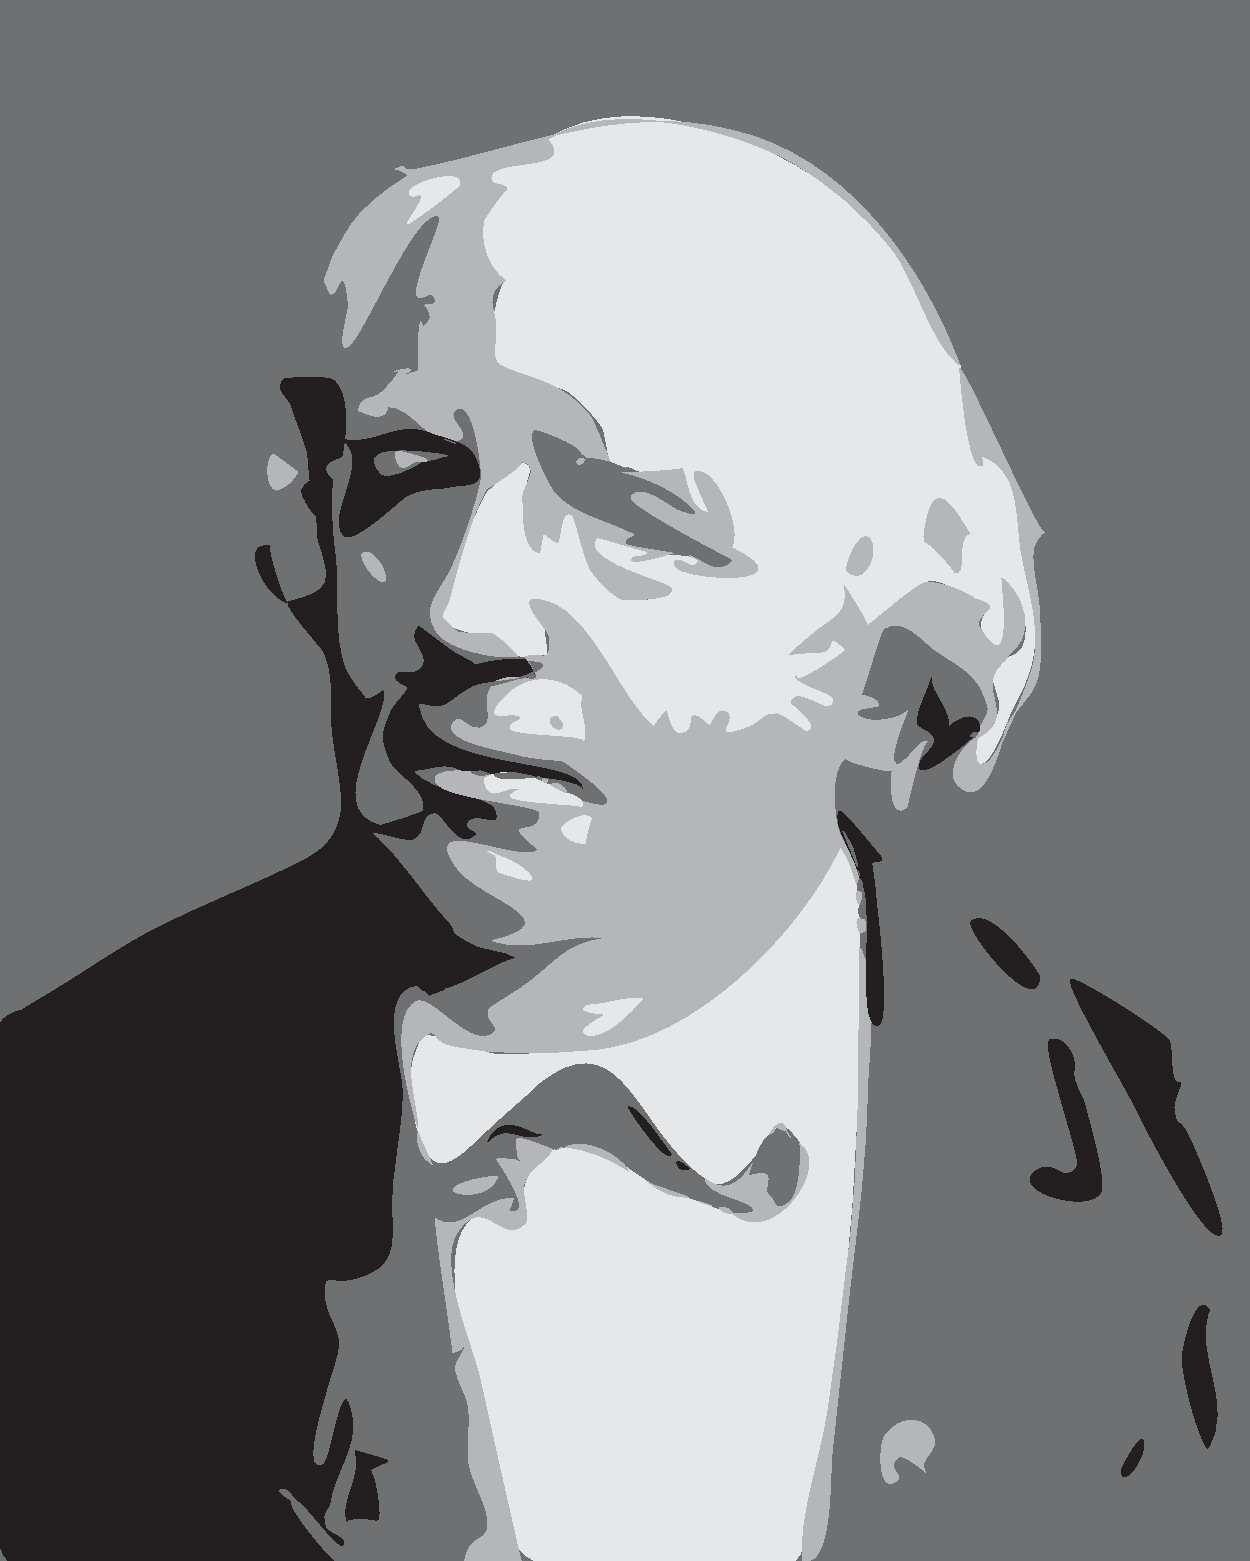
\includegraphics[width=.3\textwidth]{./fotos/calcasdos/Weierstrass.pdf}\\[5pt]
 {\small\bfseries Karl Weierstrass}
\end{bio}

La noción de continuidad de una función entre espacios
métricos es formalmente idéntica a la de continuidad de una
función entre espacios euclidianos que ya conocemos. En este
capítulo estudiaremos este concepto y daremos varias
caracterizaciones de la continuidad.

\section{Definiciones y ejemplos}

Sean $X=(X,d_{X})$ y $Y=(Y,d_{Y})$ espacios métricos.

\begin{definition}
  \label{2.1.1}Una función $\phi\colon X\rightarrow Y$ es
  \textbf{continua en el punto\ }$x_{0}\in X$ si, para cada
  $\varepsilon >0$, existe $\delta >0$ (que depende de $x_{0}$ y de
  $\varepsilon $) tal que
  \begin{equation*}
    d_{Y}(\phi (x),\phi (x_{0}))<\varepsilon \text{\qquad si \ }d_{X}(x,x_{0})<\delta.
  \end{equation*}
  Decimos que $\phi $ es \textbf{continua}
  \index{función!continua}si lo es en todo punto de $X$.
\end{definition}

La continuidad de $\phi $ depende de las métricas que estamos
considerando en $X$ y $Y$. Para hacer énfasis en ello usaremos en
ocasiones la notación
\begin{equation*}
  \phi\colon (X,d_{X})\rightarrow (Y,d_{Y})
\end{equation*}
en vez de $\phi\colon X\rightarrow Y$. Veamos algunos ejemplos.

\begin{example}
  \label{idR}La identidad $\id\colon \mathbb{R}_{p}^{n}\rightarrow
  \mathbb{R}_{r}^{n}$ es una función continua para cualesquiera
  $p,r\in [1,\infty ]$.
\end{example}

\begin{proof}
  Observa que $\left( \max \left\{ a_{1}^{r},\ldots ,a_{n}^{r}\right\}
  \right)^{1/r}=\max \left\{ a_{1},\ldots ,a_{n}\right\} $ si $r\in
  [1,\infty ) $ y $a_{1},\ldots ,a_{n}\geq 0$. En consecuencia,
  para cualesquiera $p,r\in [1,\infty )$ y $x=(x_{1},\ldots
  ,x_{n})\in \mathbb{R}^{n}$ se tiene que
  \begin{equation*}
      \begin{aligned}
        &\left\Vert x\right\Vert_{r}=\biggl( \sum_{i=1}^{n}\left\vert
            x_{i}\right\vert^{r}\biggr)^{1/r}\leq \left( n\max_{i=1,\ldots
            ,n}\left\vert x_{i}\right\vert^{r}\right)^{1/r}=n^{1/r}\max_{i=1,\ldots
          ,n}\left\vert x_{i}\right\vert =n^{1/r}\left\Vert x\right\Vert_{\infty },
        \\ 
        &\left\Vert x\right\Vert_{\infty }=\max_{i=1,\ldots ,n}\left\vert
          x_{i}\right\vert =\left( \max_{i=1,\ldots ,n}\left\vert x_{i}\right\vert
         ^{p}\right)^{1/p}\leq \biggl( \sum_{i=1}^{n}\left\vert
            x_{i}\right\vert^{p}\biggr)^{1/p}=\left\Vert x\right\Vert_{p}.
      \end{aligned}
  \end{equation*}
  Combinando ambas desigualdades obtenemos
  \begin{equation}
    \left\Vert x\right\Vert_{r}\leq n^{1/r}\left\Vert x\right\Vert_{p},\text{\quad }\left\Vert x\right\Vert_{\infty }\leq \left\Vert x\right\Vert
   _{p},\text{\quad }\forall x\in \mathbb{R}^{n},\text{ \ }p\in [1,\infty ],\text{ \ }r\in [1,\infty ).  \label{Rn}
  \end{equation}
  Dados $x_{0}\in \mathbb{R}^{n}$ y $\varepsilon >0$ definimos $\delta
  :=n^{-1/r}\varepsilon $ si $r\in [1,\infty )$ \ y $\delta
  :=\varepsilon $ si $r=\infty $. De las desigualdades (\ref{Rn}) se
  sigue que
  \begin{equation*}
    \left\Vert x-x_{0}\right\Vert_{r}<\varepsilon \text{\qquad si }\left\Vert
      x-x_{0}\right\Vert_{p}<\delta .
  \end{equation*}
  Esto prueba que $\id\colon\mathbb{R}_{p}^{n}\rightarrow
  \mathbb{R}_{r}^{n}$ es continua.
\end{proof}

\begin{example}
  \label{idC1inf}La identidad $\id\colon\mathcal{C}_{\infty
  }^{0}[0,1]\rightarrow \mathcal{C}_{1}^{0}[0,1]$ es continua,
  mientras que la identidad $\id\colon\mathcal{C}_{1}^{0}[0,1]\rightarrow
  \mathcal{C}_{\infty }^{0}[0,1]$ no lo es.
\end{example}

\begin{proof}
  La Proposición~\ref{compinorm} asegura que
  \begin{equation*}
    \left\Vert f\right\Vert_{1}\leq \left\Vert f\right\Vert_{\infty }\text{\qquad }\forall f\in \mathcal{C}^{0}[0,1].
  \end{equation*}
  En consecuencia, dadas $f_{0}\in \mathcal{C}^{0}[0,1]$ y
  $\varepsilon >0$, para $\delta =\varepsilon $ se cumple que
  \begin{equation*}
    \left\Vert f-f_{0}\right\Vert_{1}<\varepsilon \text{\qquad si }\left\Vert
      f-f_{0}\right\Vert_{\infty }<\delta .
  \end{equation*}
  Esto prueba que $\id\colon\mathcal{C}_{\infty }^{0}[0,1]\rightarrow
  \mathcal{C}_{1}^{0}[0,1]$ es continua.

  Denotemos por $0$ a la función constante con valor $0$ en
  $[0,1]$. Probaremos que $\id\colon\mathcal{C}_{1}^{0}[0,1]\rightarrow
  \mathcal{C}_{\infty }^{0}[0,1]$ no es continua en $0$ (de hecho no
  lo es en ningún punto de $\mathcal{C}^{0}[0,1]$). Sea
  $\varepsilon :=\frac{1}{2}$. Afirmamos que para cualquier $\delta
  \in (0,1)$ existe $g_{\delta }\in \mathcal{C}^{0}[0,1]$ tal que
  $\left\Vert g_{\delta }\right\Vert_{1}<\delta $ y $\left\Vert
    g_{\delta }\right\Vert_{\infty }=1>\varepsilon $. En efecto, la
  función
  \begin{equation*}
    g_{\delta }(x)=
      \begin{cases}
        1-\frac{1}{\delta }x & \text{si $0\leq x\leq \delta$,} \\ 
        0 & \text{si $\delta \leq x\leq 1$,}
      \end{cases}
  \end{equation*}
  tiene estas propiedades.
  \begin{figure}[H]
    \centering
    \begin{tikzpicture}[domain=-.1:1.2,scale=2]
  \draw (-.05,0)--(1.1,0);
  \draw (0,-.05)--(0,1.1);
  \draw[very thick] (0,1)--(.25,0)--(1,0);
  \foreach \x in {0.25, 0.5, 0.75, 1}{
               \draw[thin] (\x,-0.05)--(\x,0);
               \draw[thin] (-.05,\x)--(0,\x);
};
\draw (.15,.6) node[right] {$y=g_{\delta}(x)$};
% \draw (0,-.05) node[below] {$0$};
 \draw (.25,-.05) node[below] {$\delta$};
% \draw (.5,-.05) node[below] {$\frac{1}{2}$};
% \draw (.75,-.05) node[below] {$\frac{3}{4}$};
% \draw (1,-.05) node[below] {$1$};
% \draw (-.05,0) node[left] {$0$};
% \draw (-.05,.25) node[left] {$\frac{1}{4}$};
% \draw (-.05,.5) node[left] {$\frac{1}{2}$};
% \draw (-.05,.75) node[left] {$\frac{3}{4}$};
% \draw (-.05,1) node[left] {$1$};
\end{tikzpicture}

    % \caption{}
  \end{figure}
  \noindent
  Por tanto, la identidad $\id\colon\mathcal{C}_{1}^{0}[0,1]\rightarrow
  \mathcal{C}_{\infty }^{0}[0,1]$ no es continua en $0$.
\end{proof}

\begin{definition}
  Una función $\phi\colon X\rightarrow Y$ es un \textbf{homeomorfismo}
  \index{homeomorfismo}si $\phi $ es continua y biyectiva y su inversa
  $\phi^{-1}\colon Y\rightarrow X$ es continua. Se dice que $X$ y $Y$ son
  \textbf{homeomorfos} si existe un homeomorfismo entre ellos.
\end{definition}

Los ejemplos anteriores afirman que $\id\colon\mathbb{R}_{p}^{n}\rightarrow
\mathbb{R}_{r}^{n}$ es un homeomorfismo para cualesquiera $p,r\in
[1,\infty ]$, mientras que $\id\colon\mathcal{C}_{\infty
}^{0}[a,b]\rightarrow \mathcal{C}_{1}^{0}[a,b]$ no lo es.

\begin{proposition}
  \label{homeocont}Sean $\phi\colon X\rightarrow Y$ y $\psi\colon Y\rightarrow
  Z$ funciones entre espacios métricos.

  \begin{enumerate}
  \item[(a)] Si $\phi $ y $\psi $ son continuas entonces la
    composición $\psi \circ \phi\colon X\rightarrow Z$ es continua.

  \item[(b)] Si $\phi $ es un homeomorfismo, entonces $\psi $ es
    continua si y sólo si $\psi \circ \phi $ es continua.

  \item[(c)] Si $\psi $ es un homeomorfismo, entonces $\phi $ es
    continua si y sólo si $\psi \circ \phi $ es continua.
  \end{enumerate}
\end{proposition}

\begin{proof}
  \emph{(a):} Sean $x_{0}\in X$ y $\varepsilon >0$. Como $\psi $ es
  continua en $y_{0}:=\phi (x_{0})$, existe $\gamma >0$ tal que
  \begin{equation*}
    d_{Z}(\psi (y),\psi (y_{0}))<\varepsilon 
    \text{\qquad si \ }d_{Y}(y,y_{0})<\gamma .
  \end{equation*}
  Y, como $\phi $ es continua en $x_{0}$, existe $\delta >0$ tal que
  \begin{equation*}
    d_{Y}(\phi (x),\phi (x_{0}))<\gamma \text{\qquad si \ }d_{X}(x,x_{0})<\delta
    .
  \end{equation*}
  En consecuencia,
  \begin{equation*}
    d_{Z}(\psi (\phi (x)),\psi (\phi (x_{0})))<\varepsilon \text{\qquad si \ }d_{X}(x,x_{0})<\delta .
  \end{equation*}
  Es decir, $\psi \circ \phi\colon X\rightarrow Z$ es continua.

  \emph{(b):} Si $\phi $ es un homeomorfismo, de la afirmación
  \emph{(a)} se sigue que $\psi \circ \phi $ es continua si y sólo
  si $\left( \psi \circ \phi \right) \circ \phi^{-1}=\psi $ lo es.

  \emph{(c):} Análogamente, si $\psi $ es un homeomorfismo,
  entonces $\psi \circ \phi $ es continua si y sólo si $\psi
 ^{-1}\circ \left( \psi \circ \phi \right) =\phi $ lo es.
\end{proof}

La proposición anterior nos permite concluir que
$f\colon\mathbb{R}^{n}\rightarrow \mathbb{R}^{m}$ es continua si y sólo
si $f\colon\mathbb{R}_{p}^{n}\rightarrow \mathbb{R}_{r}^{m}$ es continua
para cualesquiera $p,r\in [1,\infty ]$ [Ejercicio
\ref{contRn}].

Algunas propiedades importantes de los espacios métricos, como la
completitud (que estudiaremos más adelante), no se preservan bajo
homeomorfismos. Por ello conviene introducir los siguientes conceptos.

\begin{definition}
  Una función $\phi\colon X\rightarrow Y$ es \textbf{Lipschitz
    continua}, \index{función!Lipschitz continua}si existe $c>0$
  tal que
  \begin{equation*}
    d_{Y}(\phi (x),\phi (y))\leq c\,d_{X}(x,y)\text{\qquad }\forall x,y\in X.
  \end{equation*}
  La constante $c$ se llama una \textbf{constante de
    Lipschitz}\footnote{Rudolf Otto Sigismund Lipschitz (1832-1903)
    nació en Königsberg (entonces parte de Alemania). Se
    doctoró en Berlín bajo la supervisión de Lejeune
    Dirichlet. Fue profesor en la Universidad de Bonn.} para $\phi $.

  La función $\phi $ es una \textbf{equivalencia}
  \index{equivalencia}si $\phi $ es Lipschitz continua y biyectiva y
  su inversa $\phi^{-1}\colon Y\rightarrow X$ es Lipschitz continua.
\end{definition}

\begin{bio}
  \centering
  
\includegraphics[width=.3\textwidth]{./fotos/calcasdos/Lipschitz.pdf}\\[5pt]
  {\small\bfseries Rudolf Lipschitz}
\end{bio}
Esta noción es más fuerte que la de continuidad, es decir, se
cumple lo siguiente.

\begin{proposition}
  \label{lip-cont}Si $\phi $ es Lipschitz continua entonces $\phi $ es
  continua.
\end{proposition}

\begin{proof}
  Sea $c>0$ una constante de Lipschitz para $\phi $. Entonces, dada
  $\varepsilon >0$, para $\delta :=\frac{\varepsilon }{c}>0$ se cumple
  que
  \begin{equation*}
    d_{Y}(\phi (x),\phi (x_{0}))<\varepsilon \text{\qquad si }d_{X}(x,x_{0})<\delta .
  \end{equation*}
  Por tanto, $\phi $ es continua.
\end{proof}

Nota que en este caso $\delta $ no depende del punto $x_{0}\in X$. El
inverso no es cierto en general, es decir, no toda función
continua es Lipschitz continua [Ejercicio~\ref{lip}].

\begin{definition}
  Dos métricas $d_{1}$ y $d_{2}$ en un conjunto $X$ son
  \textbf{equivalentes} \index{metricas@métricas equivalentes}si la
  identidad $\id\colon (X,d_{1})\rightarrow (X,d_{2})$ es una equivalencia,
  es decir, si existen constantes $c_{1},c_{2}>0$ tales que
  \begin{equation*}
    c_{1}\,d_{2}(x,y)\leq d_{1}(x,y)\leq c_{2}\,d_{2}(x,y)\text{\qquad }\forall x,y\in X.
  \end{equation*}
  Análogamente, dos normas $\left\Vert \cdot \right\Vert_{1}$ y
  $\left\Vert \cdot \right\Vert_{2}$ en un espacio vectorial $V$ son
  \textbf{equivalentes} \index{normas equivalentes}si las métricas
  inducidas son equivalentes, es decir, si existen constantes
  $c_{1},c_{2}>0$ tales que
  \begin{equation*}
    c_{1}\,\left\Vert v\right\Vert_{2}\leq \left\Vert v\right\Vert_{1}\leq
    c_{2}\,\left\Vert v\right\Vert_{2}\text{\qquad }\forall v\in V.
  \end{equation*}
\end{definition}

Las desigualdades (\ref{Rn}) muestran que $\left\Vert \cdot
\right\Vert_{p}$ y $\left\Vert \cdot \right\Vert_{r}$ son normas
equivalentes en $\mathbb{R}^{n}$ para cualesquiera $p,r\in [1,\infty ]$, mientras que el Ejemplo~\ref{idC1inf} muestra que
$\left\Vert \cdot \right\Vert_{1}$ y $\left\Vert \cdot \right\Vert
_{\infty }$ no son normas equivalentes en $\mathcal{C}^{0}[0,1]$. De
hecho, $\left\Vert \cdot \right\Vert_{p}$ y $\left\Vert \cdot
\right\Vert_{r}$ no son normas equivalentes en $\mathcal{C}^{0}[a,b]$
para ningún par de números $1\leq p<r\leq \infty $ [Ejercicio
\ref{ejidC}].

La siguiente noción nos permite visualizar el concepto de
continuidad.

\begin{definition}
  \label{defbolaab}Sean $X=(X,d_{X})$ un espacio métrico,
  $x_{0}\in X$ y $\varepsilon >0$. La \textbf{bola abierta\
  }\index{bola!abierta@abierta $B_{X}(x,\varepsilon )$}en $X$ con
  centro en $x_{0}$\ y radio $\varepsilon $ es el conjunto
  \begin{equation*}
    B_{X}(x_{0},\varepsilon ):=\left\{ x\in X:d_{X}(x,x_{0})<\varepsilon
    \right\} .
  \end{equation*}
\end{definition}

Dados un subconjunto $A$ de $X$ y una función $\phi\colon X\rightarrow
Y$, denotamos por
\begin{equation*}
  \phi (A):=\left\{ \phi (x)\in Y:x\in A\right\}
\end{equation*}
a la \textbf{imagen de} $A$ \textbf{bajo} $\phi $. \index{imagen!de un
  conjunto@de un conjunto $\phi (A)$}Con estos conceptos podemos
reformular la definición de continuidad como sigue:

$\phi\colon X\rightarrow Y$ \emph{es} \textbf{continua en el punto} $x_{0}$
\emph{de} $X$ \emph{si, dada }$\varepsilon >0$,\emph{\ existe }$\delta
>0$\emph{\ tal que}
\begin{equation}
  \phi (B_{X}(x_{0},\delta ))\subset B_{Y}(\phi (x_{0}),\varepsilon ).
  \label{carcont}
\end{equation}
\begin{figure}[H]
  \centering
  \begin{tikzpicture}[scale=1]
  \pgfmathsetmacro{\hor}{0.45}
  \pgfmathsetmacro{\ver}{-0.3}
  \draw[dashed,fill=gray!25] (0,0) circle (1cm);
  \draw[dashed,fill=gray!25] (6.8,0) circle (1.5cm);
  \draw[very thin,dashed,fill=gray!50] plot[smooth cycle, tension=.9]
  coordinates{(6.1+\hor,-0.2+\ver) (7.2+\hor,0.05+\ver) (7.2+\hor,1+\ver) (6.45+\hor,.85+\ver) (5.75+\hor,.7+\ver)};
  \draw[-latex'] (0.9,.6) .. controls (2.2,1) and (4.3,1) .. 
  node[above] {$\phi$} (5.7+\hor,.6+\ver);
  \node[right] at (0,0) {$x_0$};
  \node[right] at (6.35+\hor,0.3+\ver) {$\phi(x_0)$};
  \node at (315:1.6cm) {$B_{X}(x_0,\delta)$};
  \node at (8.5,-1.5) {$B_{Y}(\phi(x_0),\varepsilon)$};
  \draw[only marks,mark=*, mark size=1.2pt] plot 
  coordinates{(0,0) (6.35+\hor,.3+\ver)};
\end{tikzpicture}

  % \caption{}
\end{figure}

Revisemos algunos de los ejemplos anteriores bajo esta nueva
óptica.

\begin{example}
  \label{Rbolas}Denotemos por $B_{p}(x_{0},\varepsilon )$ a la bola
  abierta en $\mathbb{R}_{p}^{n}$ con centro en $x_{0}$ y radio
  $\varepsilon $.
\begin{figure}[H]
  \centering
  \begin{tikzpicture}[scale=1]
  \draw[dashed,fill=gray!25] (0,0) circle (1cm);
  \draw[dashed,fill=gray!25] (-2.5,0) -- (-3.5,1) -- (-4.5,0) -- (-3.5,-1) --cycle;
  \draw[dashed,fill=gray!25] (2.5,1) -- (2.5,-1) -- (4.5,-1) -- (4.5,1) --cycle;
  \foreach \x in {0, -3.5, 3.5} {
    \draw[very thin, -latex'] ({\x - 1.25},0) -- ({\x + 1.3},0);
    \draw[very thin, -latex'] ({\x},-1.25) -- ({\x},1.3);
  }
\node[below] at (-3.5,-1.3) {$B_1(0,1)$};
\node[below] at (0,-1.3) {$B_2(0,1)$};
\node[below] at (3.5,-1.3) {$B_\infty(0,1)$};
\end{tikzpicture}

  % \caption{}
\end{figure}
\noindent
  De las desigualdades \emph{(\ref{Rn})} se sigue que existe $c>0$
  (que depende de $n$ y $r$) tal que
  \begin{equation*}
    B_{p}(x_{0},c\varepsilon )\subset B_{r}(x_{0},\varepsilon )\qquad
    \forall p,r\in [1,\infty ],\text{ \ }\forall x_{0}\in \mathbb{R}^{n}.
  \end{equation*}
  La caracterización \emph{(\ref{carcont})} de la continuidad
  asegura entonces que $\id\colon\mathbb{R}_{p}^{n}\rightarrow
  \mathbb{R}_{r}^{n}$ es un homeomorfismo.
\end{example}

\begin{example}
  \label{Cbolas}Denotemos por $B_{p}(f_{0},\varepsilon )$ a la bola
  abierta en $\mathcal{C}_{p}^{0}[0,1]$ con centro en la función
  continua $f_{0}\colon [0,1]\rightarrow \mathbb{R}$ y radio $\varepsilon $.
  Si $p=\infty $,
  \begin{equation*}
    B_{\infty }(f_{0},\varepsilon )=\left\{f\in \mathcal{C}^{0}[0,1]:\left\vert
      f(x)-f_{0}(x)\right\vert <\varepsilon \text{ \ }\forall x\in [0,1]\right\},
  \end{equation*}
  es decir, $B_{\infty }(f_{0},\varepsilon )$ es el conjunto de las
  funciones continuas cuya gráfica está contenida en la franja
  $\left\{ (x,y)\in \mathbb{R}^{2}:x\in [0,1],\; 
\left\vert y-f_{0}(x)\right\vert <\varepsilon \right\}$.
\begin{figure}[H]
  \centering
  \begin{tikzpicture}[scale=1]
\foreach \x in {0,.8}
\draw[dashed] plot[smooth, tension=0.7] coordinates{(-2,{\x + 2.1}) (-1,{\x + 2.5}) (1,{\x + 1.5}) (2,{\x + 1.9})};
\draw plot[smooth,tension=0.7] coordinates{(-2,{.4 + 2.1}) (-1,{.4 + 2.5}) (1,{.4 + 1.5}) (2,{.4 + 1.9})};
\draw[thick] plot[mark=*, mark size=1pt,ScalePlotMarksOff] coordinates {(-2,1) (2,1)};
\node[below] at (-2,.95) {$0$};
\node[below] at (2,.95) {$1$};

\end{tikzpicture}

  % \caption{}
\end{figure}
\noindent
  Por otra parte, si $p=1$,
  \begin{equation*}
    B_{1}(f_{0},\varepsilon )=\left\{g\in \mathcal{C}^{0}[0,1]:\int_{0}^{1}\left\vert
      g(x)-f_{0}(x)\right\vert dx<\varepsilon \right\}
  \end{equation*}
  es el conjunto de las funciones continuas $g$ tales que el área
  de la región comprendida entre las gráficas de $g$ y $f_{0}$
  es menor que $\varepsilon $.

  Resulta claro entonces que $B_{\infty }(f_{0},\varepsilon )\subset
  B_{1}(f_{0},\varepsilon )$. Y también que, para cada
  $\varepsilon >0$ y cada $\delta >0$, podemos encontrar una
  función continua $g$ tal que $g\in B_{1}(f_{0},\delta )$ pero
  $g\notin B_{\infty }(f_{0},\varepsilon )$:
\begin{figure}[H]
  \centering
  \begin{tikzpicture}[scale=1]
\foreach \x in {0,.8}
\draw[dashed] plot[smooth, tension=0.7] coordinates{(-2,{\x + 2.1}) (-1,{\x + 2.5}) (1,{\x + 1.5}) (2,{\x + 1.9})};
\draw plot[smooth,tension=0.7] coordinates{(-2,{.4 + 2.1}) (-1,{.4 + 2.5}) (1,{.4 + 1.5}) (2,{.4 + 1.9})};
\draw[thick] (-2,{.35 + 2.1})% .. controls (-1.7,3) and (-1.4,3.2) .. (-1.3,{.4 + 2.5})
.. controls (-1.2,3.4) and (-0.3,2.8) .. (-0.1,2.45)
.. controls (-.07,2.4) and (-0.02,2.4) .. (-0.01,3.5) 
.. controls (-0.01,3.6) and (0.01,3.6) .. (0.01,3.5)
.. controls (0.02,2.5) and (.07,2.4) .. (.1,2.35) 
.. controls (0.3,2) and (1.2,1.4) .. (2,{.45 + 1.9});

\draw[thick] plot[mark=*, mark size=1pt, ScalePlotMarksOff] coordinates {(-2,1) (2,1)};
\node[below] at (-2,.95) {$0$};
\node[below] at (2,.95) {$1$};
\node[right] at (0,3.25) {$y=g(x)$};
\end{tikzpicture}

  % \caption{}
\end{figure}
\noindent
  De la caracterización \emph{(\ref{carcont})} de la continuidad
  se sigue que $\id\colon \mathcal{C}_{\infty }^{0}[0,1]\rightarrow
  \mathcal{C}_{1}^{0}[0,1]$ es continua y que
  $\id\colon \mathcal{C}_{1}^{0}[0,1]\rightarrow \mathcal{C}_{\infty
  }^{0}[0,1]$ no lo es.
\end{example}

\section{Conjuntos abiertos y conjuntos cerrados}

Sea $X=(X,d)$ un espacio métrico y sea $A$ un subconjunto de $X$.

\begin{definition}
  \label{defint}Un punto $x\in X$ se llama un \textbf{punto interior}
  \index{punto!interior}\textbf{de} $A$ si existe $\varepsilon >0$ tal
  que $B_{X}(x,\varepsilon )\subset A$. El conjunto de todos los
  puntos interiores de $A$ se llama el \textbf{interior de
  }$A$\textbf{\ en }$X$ \index{interior!interior@int$(A)$,
    $\Int_{X}(A)$}y se denota $\Int_{X}(A)$, o simplemente
  $\Int(A)$. Decimos que $A$ es \textbf{abierto}
  \index{conjunto!abierto}\textbf{en} $X$ si $A=\Int(A)$.
\end{definition}

Observa que $\Int_{X}(A)\subset A$. Veamos que la bola abierta es un
abierto en este sentido.

\begin{proposition}
  \label{bolaabab}En cualquier espacio métrico $X=(X,d)$, la bola
  abierta
  \begin{equation*}
    B_{X}(x_{0},\varepsilon ):=\left\{ x\in X:d(x,x_{0})<\varepsilon \right\}
  \end{equation*}
  con centro en $x_{0}$ y radio $\varepsilon $ es un subconjunto
  abierto de $X. $
\end{proposition}

\begin{proof}
  Sea $x\in B_{X}(x_{0},\varepsilon )$. Tomemos $\delta :=\varepsilon
  -d(x,x_{0})>0$. Para todo $z\in B_{X}(x,\delta )$, se cumple que
  \begin{equation*}
    d(z,x_{0})\leq d(z,x)+d(x,x_{0})<\delta +d(x,x_{0})=\varepsilon ,
  \end{equation*}
  es decir, $z\in B_{X}(x_{0},\varepsilon )$. Por tanto,
  $B_{X}(x,\delta )\subset B_{X}(x_{0},\varepsilon )$.
\begin{figure}[H]
  \centering
  \begin{tikzpicture}[scale=.8]
\draw[dashed, fill=gray!25] (0,0) circle [radius=2cm];
\draw[dashed, fill=gray!50, rotate=60] (.8,0) circle [radius=1.2cm];
\draw[only marks, mark=*, mark size=1pt, ScalePlotMarksOff] plot (0,0);
\draw[only marks, mark=*, mark size=1pt, ScalePlotMarksOff, rotate=60] plot (.8,0);
\draw[only marks, mark=*, mark size=1pt, ScalePlotMarksOff, rotate=60] node[right] at (.8,0) {$x$};
\node[right] at (0,0) {$x_0$};
\end{tikzpicture}

  % \caption{}
\end{figure}
\noindent
  Esto muestra que $x\in\Int(B_{X}(x_{0},\varepsilon ))$ para todo
  $x\in B_{X}(x_{0},\varepsilon )$. En consecuencia
  $B_{X}(x_{0},\varepsilon )=\Int(B_{X}(x_{0},\varepsilon ))$.
\end{proof}

\begin{corollary}
  \label{intab}El interior $\Int(A)$ de cualquier subconjunto
  $A$ de $X$ es abierto en $X$.
\end{corollary}

\begin{proof}
  Sea $x\in\Int(A)$. Entonces existe $\varepsilon >0$ tal que
  $B_{X}(x,\varepsilon )\subset A$. Probaremos ahora que
  $B_{X}(x,\varepsilon )\subset\Int A$. En efecto, por la
  Proposición~\ref{bolaabab}, para cada $z\in B_{X}(x,\varepsilon
  )$ existe $\delta >0$ tal que $B_{X}(z,\delta )\subset
  B_{X}(x,\varepsilon )\subset A$. Por tanto, $z\in\Int A$.
\end{proof}

Es fácil ver que $\Int(A)$ es el mayor subconjunto abierto de $X$
contenido en $A$ [Ejercicio~\ref{ejmaxint}].

El que un subconjunto $A$ de $X$ sea abierto en $X$ o no lo sea
depende de la métrica que le demos a $X$. Veamos un ejemplo.

\begin{example}
  El conjunto
  \begin{equation*}
    A:=\left\{f\in \mathcal{C}^{0}[0,1]:\left\vert f(x)\right\vert <\tfrac{1}{2}\text{
      \ }\forall x\in [0,1]\right\}
  \end{equation*}
  es abierto en $\mathcal{C}_{\infty }^{0}[0,1]$, pero no es abierto
  en $\mathcal{C}_{1}^{0}[0,1]$.
\end{example}

\begin{proof}
  Observa que $A=B_{\mathcal{C}_{\infty
    }^{0}[0,1]}(0,\frac{1}{2})$. La Proposición~\ref{bolaabab}
  asegura que $A$ es abierto en $\mathcal{C}_{\infty }^{0}[0,1]$.

  Probaremos ahora que $A$ no es abierto en
  $\mathcal{C}_{1}^{0}[0,1]$. Para cada $0<\delta <1$ consideremos la
  función
  \begin{equation*}
    g_{\delta }(x)=
      \begin{cases}
        1-\frac{1}{\delta }x & \text{si $0\leq x\leq \delta$,} \\ 
        0 & \text{si $\delta \leq x\leq 1$.}
      \end{cases}
  \end{equation*}
  Entonces $\left\Vert g_{\delta }\right\Vert_{1}=\frac{\delta }{2}$
  y $\left\Vert g_{\delta }\right\Vert_{\infty }=1$. Por tanto,
  $g_{\delta }\in B_{\mathcal{C}_{1}^{0}[0,1]}(0,\delta )$, pero
  $g_{\delta }\not\in A$.
\begin{figure}[H]
  \centering
  \begin{tikzpicture}[scale=1.5]
\foreach \x in {-.5, .5}
\draw[dashed] (0,{\x}) -- (2.5,{\x});
\draw (0,0) -- (2.5,0);
\draw[-latex] (0,-.7) -- (0,1.2);
\draw[very thick] (0,1) -- (.25,0) -- (2.5,0);
\node[left] at (0,-.5) {$-\frac{1}{2}$}; 
\node[left] at (0,0) {$0$}; 
\node[left] at (0,.5) {$\frac{1}{2}$};
\node[right] at (.05,.8) {$y=g_\delta(x)$}; 
\end{tikzpicture}

  % \caption{}
\end{figure}
\noindent
  Es decir, $B_{\mathcal{C}_{1}^{0}[0,1]}(0,\delta )$ no está
  contenida en $A$ para ningún $\delta >0$. En consecuencia, la
  función $0$ no es un punto interior de $A$ en
  $\mathcal{C}_{1}^{0}[0,1]$.
\end{proof}

De hecho, el conjunto $A$ del ejemplo anterior tiene interior
vacío en $\mathcal{C}_{1}^{0}[0,1]$ \ [Ejercicio~\ref{ejintbola}].

\begin{definition}
  \label{defcerradura}Un punto $x\in X$ se llama un \textbf{punto de
    contacto de} $A$ \index{punto!de contacto}si $B_{X}(x,\varepsilon
  )\cap A\neq \emptyset $ para toda $\varepsilon >0$. El conjunto de
  todos los puntos de contacto de $A $ se llama la \textbf{cerradura}
  \index{cerradura!cerradura@$\overline{A}$, $\cerr_{X}(A)$}\textbf{de}
  $A$ \textbf{en} $X$ y se denota $\cerr_{X}(A)$, o simplemente
  $\overline{A}$. Decimos que $A$ es \textbf{cerrado en} $X$
  \index{conjunto!cerrado}si $A=\overline{A}$.
\end{definition}

Nota que todo punto de $A$ es punto de contacto de $A$, es decir,
$A\subset \overline{A}$.

\begin{definition}
  La \textbf{bola cerrada} en $X$\ \index{bola!cerrada@cerrada
    $\bar{B}_{X}(x,\varepsilon )$}con centro en $x_{0}$\ y radio
  $\varepsilon $ es el conjunto
  \begin{equation*}
    \bar{B}_{X}(x_{0},\varepsilon ):=\left\{ x\in X:d(x,x_{0})\leq \varepsilon
    \right\} .
  \end{equation*}
\end{definition}

\begin{proposition}
  $\bar{B}_{X}(x_{0},\varepsilon )$ es un subconjunto cerrado de $X$.
\end{proposition}

\begin{proof}
  Sea $x\in \overline{\bar{B}_{X}(x_{0},\varepsilon )}$. Entonces,
  para todo $\delta >0$, existe $x_{\delta }\in B_{X}(x,\delta )\cap
  \bar{B}_{X}(x_{0},\varepsilon )$. De la desigualdad del
  triángulo se sigue que
  \begin{equation*}
    d(x,x_{0})\leq d(x,x_{\delta })+d(x_{\delta },x_{0})<\delta +\varepsilon 
    \text{\qquad }\forall \delta >0.
  \end{equation*}
  En consecuencia $d(x,x_{0})\leq \varepsilon $, es decir, $x\in
  \bar{B}_{X}(x_{0},\varepsilon )$.
\end{proof}

Denotaremos por $X\smallsetminus A$ al \textbf{complemento}
\index{complemento!de un conjunto@de un conjunto $X\smallsetminus
  A$}\textbf{de} $A$ \textbf{en} $X$, es decir,
\begin{equation*}
  X\smallsetminus A:=\left\{ x\in X:x\notin A\right\} .
\end{equation*}
Los abiertos y los cerrados son duales en el siguiente sentido.

\begin{proposition}
  \label{abcer}Para cualquier subconjunto $A$ de un espacio
  métrico $X$ se cumple que
  \begin{equation*}
    X\smallsetminus 
    \overline{A}=\emph{int}(X\smallsetminus A).
  \end{equation*}
  En consecuencia, $A$ es cerrado en $X$ si y sólo si
  $X\smallsetminus A$ es abierto en $X$.
\end{proposition}

\begin{proof}
  La primera afirmación es inmediata. En efecto,
  $x\in\Int(X\smallsetminus A)$ si y sólo si existe $\varepsilon >0$
  tal que $B_{X}(x,\varepsilon )\cap A=\emptyset $, es decir, si y
  sólo si $x\in X\smallsetminus \overline{A}$.

  En consecuencia, si $A$ es cerrado, entonces $X\smallsetminus
  A=X\smallsetminus \overline{A}=\Int(X\smallsetminus A)$, es decir,
  $X\smallsetminus A$ es abierto. E inversamente, si $X\smallsetminus
  A$ es abierto, entonces $X\smallsetminus A=\Int(X\smallsetminus
  A)=X\smallsetminus \overline{A}$ y, en consecuencia,
  $A=\overline{A}$, es decir, $A$ es cerrado.
\end{proof}

\begin{corollary}
  La cerradura $\overline{A}$ de cualquier subconjunto $A$ de $X$ es
  cerrada en $X$.
\end{corollary}

\begin{proof}
  Por el Corolario~\ref{intab} sabemos que $\Int(X\smallsetminus A)$ es
  abierto en $X$. En consecuencia, por la Proposición~\ref{abcer},
  se tiene que $\overline{A}=X\smallsetminus\Int(X\smallsetminus
  A)$ es cerrado en~$X$.
\end{proof}

Es sencillo comprobar que $\overline{A}$ es el menor subconjunto
cerrado de $X$ que contiene a~$A$ [Ejercicio~\ref{ejmincer}].

Existen subconjuntos que no son ni abiertos ni cerrados. Por ejemplo,
el intervalo $[a,b)$ no es ni abierto ni cerrado en
$\mathbb{R}$. Más aún, un subconjunto puede ser
simultáneamente abierto y cerrado como lo muestra el siguiente
ejemplo.

\begin{example}
  Todo subconjunto de un espacio métrico discreto $X_{\disc}$ es
  abierto en $X_{\disc}$. En consecuencia, todo subconjunto de
  $X_{\disc}$ es cerrado en $X_{\disc}$.
\end{example}

\begin{proof}
  Observemos que, para cada punto $x\in X$,
  \begin{equation*}
    B_{\disc}(x,1):=\left\{y\in X:d_{\disc}(y,x)<1\right\}=\left\{x\right\}.
  \end{equation*}
  Para cualquier subconjunto $A$ de $X$ se tiene entonces que
  $B_{\disc}(x,1)\subset A$ para todo $x\in A$. Por tanto, $A$ es
  abierto en $X_{\disc}$. De la Proposición~\ref{abcer} se sigue
  que $A$ también es cerrado en $X_{\disc}$.
\end{proof}

En general no es cierto que la cerradura de una bola abierta sea la
correspondiente bola cerrada. Veamos un ejemplo.

\begin{example}
  \label{discabcer}Si $X_{\disc}$ es un espacio métrico discreto
  con al menos dos puntos entonces, puesto que todos los subconjuntos
  de $X_{\disc}$ son cerrados, se tiene que
  \begin{equation*}
    \overline{B_{\disc}(x,1)}=B_{\disc}(x,1)=\left\{x\right\}\text{\qquad }\forall x\in X.
  \end{equation*}
  Por otra parte,
  \begin{equation*}
    \bar{B}_{\disc}(x,1):=\left\{y\in X:d_{\disc}(y,x)\leq 1\right\}=X\text{\qquad }\forall
    x\in X.
  \end{equation*}
\end{example}

Esto no ocurre en un espacio normado.

\begin{proposition}
  \label{evnbolacer}Si $V=(V,\left\Vert \cdot \right\Vert )$ es un
  espacio normado, entonces la cerradura de la bola abierta
  $B(v_{0},\varepsilon ):=\left\{ v\in V:\left\Vert v-v_{0}\right\Vert
    <\varepsilon \right\} $ es la bola cerrada
  $\bar{B}(v_{0},\varepsilon ):=\left\{ v\in V:\left\Vert
      v-v_{0}\right\Vert \leq \varepsilon \right\} $.
\end{proposition}

\begin{proof}
  Como $\bar{B}(v_{0},\varepsilon )$ es cerrado y contiene a
  $B(v_{0},\varepsilon )$ se tiene que $\overline{B(v_{0},\varepsilon
    )}\subset \bar{B}(v_{0},\varepsilon )$ [Ejercicio~\ref{ejmincer}].

  Probaremos ahora que $\bar{B}(v_{0},\varepsilon )\subset
  \overline{B(v_{0},\varepsilon )}$. Es decir, probaremos que, para
  todo $v\in \bar{B}(v_{0},\varepsilon )$ y $\delta >0$, se cumple que
  $B(v,\delta )\cap B(v_{0},\varepsilon )\neq \emptyset $. Sin perder
  generalidad podemos tomar $\delta <2\varepsilon $. El punto
  \begin{equation*}
    v_{\delta }:=v+\frac{\delta }{2\varepsilon }(v_{0}-v)\in V
  \end{equation*}
  satisface
  \begin{align*}
    \left\Vert v_{\delta }-v\right\Vert &=\frac{\delta }{2\varepsilon }\left\Vert v_{0}-v\right\Vert \leq \frac{\delta }{2}<\delta ,\text{ \ y} \\
    \left\Vert v_{\delta }-v_{0}\right\Vert &=\left(1-\frac{\delta }{2\varepsilon }\right)\left\Vert v-v_{0}\right\Vert \leq \left(1-\frac{\delta }{2\varepsilon }\right)\varepsilon <\varepsilon .
  \end{align*}
\begin{figure}[H]
  \centering
  \begin{tikzpicture}[scale=.6]
\usetikzlibrary{intersections}
  \draw [thick,fill=gray!25,name path=curve 1] (3,1) circle [radius=2.5];
  \path [name path=curve 2] (0,0) -- (6,4);
  \path [name path=curve 3] (3,1) circle [radius=1.2];
  \draw [fill=black,name intersections={of=curve 1 and curve 2, by={a,b}}]
        (a) circle (1pt);
  \path [dashed, -latex, name path=curve 4] (a) -- (3,1);
  \draw [fill=black,name intersections={of=curve 3 and curve 4, by={c}}]      
        (c) circle (1pt);
\draw[thin, dashed, -latex'] (a) -- (c);
\draw[thin, dashed, -latex'] (0,0) -- (a);
\draw[fill=black] (3,1) circle (1pt);
\draw[-latex'] (-0.1,0)--(6,0);
\draw[-latex'] (0,-1.5)--(0,3.5);
\node[right] at (3,1) {$v_0$};
\node[above right] at (a) {$v$};
\node[below right] at (c) {$v_\delta$};
\end{tikzpicture} 


  % \caption{}
\end{figure}
\noindent
  Por tanto, $v_{\delta }\in B(v,\delta )\cap B(v_{0},\varepsilon )$.
\end{proof}

Daremos ahora una caracterización de la continuidad en
términos de conjuntos abiertos y conjuntos cerrados. La
\textbf{imagen inversa} \index{imagen! inversa@inversa de un conjunto
  $\phi^{-1}(B)$}de un subconjunto $B$ de $Y$ bajo la función
$\phi\colon X\rightarrow Y$ es el conjunto
\begin{equation*}
  \phi^{-1}(B):=\left\{ x\in X:\phi (x)\in B\right\} .
\end{equation*}

\begin{proposition}
  \label{conttop}Sean $X$ y $Y$ espacios métricos, y sea $\phi\colon
  X\rightarrow Y$ una función. Las siguientes afirmaciones son
  equivalentes:

  \begin{enumerate}
  \item[(a)] $\phi\colon X\rightarrow Y$ es continua.

  \item[(b)] $\phi^{-1}(U)$ es abierto en $X$ para todo subconjunto
    abierto $U $ de $Y$.

  \item[(c)] $\phi^{-1}(C)$ es cerrado en $X$ para todo subconjunto
    cerrado $C $ de $Y$.
  \end{enumerate}
\end{proposition}

\begin{proof}
  \emph{(a) }$\Rightarrow $ \emph{(b)}: \ Sea $U$ un subconjunto
  abierto de $Y$. Para cada $x\in \phi^{-1}(U)$ tomemos $\varepsilon
  >0$ tal que $B_{Y}(\phi (x),\varepsilon )\subset U$. Como $\phi $ es
  continua, existe $\delta >0$ tal que $\phi (B_{X}(x,\delta ))\subset
  B_{Y}(\phi (x),\varepsilon )$. Entonces $B_{X}(x,\delta )\subset
  \phi^{-1}(U)$. Esto prueba que $\phi^{-1}(U)$ es abierto en $X$.

  \emph{(b) }$\Rightarrow $ \emph{(a)}: \ Sean $x\in X$ y
  $\varepsilon >0$. Como $B_{Y}(\phi (x),\varepsilon )$ es abierta en
  $Y$, se tiene que $\phi^{-1}(B_{Y}(\phi (x),\varepsilon ))$ es
  abierto en $X$. En particular, existe $\delta >0$ tal que
  $B_{X}(x,\delta )\subset \phi^{-1}(B_{Y}(\phi (x),\varepsilon ))$,
  es decir, $\phi (B_{X}(x,\delta ))\subset B_{Y}(\phi (x),\varepsilon
  )$. Esto prueba que $\phi $ es continua en $x$.

  \emph{(b) }$\Leftrightarrow $ \emph{(c)}: \ Observa que
  $X\smallsetminus \phi^{-1}(B)=\phi^{-1}(Y\smallsetminus B)$ para
  todo subconjunto $B$ de $Y$. La equivalencia entre \emph{(b) }y
  \emph{(c)} es consecuencia inmediata de la
  Proposición~\ref{abcer}. En efecto, si $\phi $ satisface \emph{(b)}
  y $C$ es cerrado en $Y$, entonces $Y\smallsetminus C$ es abierto en
  $Y$. En consecuencia, $\phi^{-1}(Y\smallsetminus C)=X\smallsetminus
  \phi^{-1}(C) $ es abierto en $X$ y, por tanto $\phi^{-1}(C)$ es
  cerrado en $X$. Esto prueba que \emph{(b) }$\Rightarrow $
  \emph{(c).} La otra implicación se demuestra de manera análoga.
\end{proof}

\begin{example}
  Cualquier función $\phi\colon X_{\disc}\rightarrow Y$ de un espacio
  métrico discreto a un espacio métrico cualquiera $Y$ es
  continua, ya que todo subconjunto de $X_{\disc}$ es abierto
  \emph{(ver Ejemplo~\ref{discabcer})}.
\end{example}

Para finalizar esta sección veamos algunas propiedades importantes
de los abiertos.

\begin{proposition}
  \label{top}En cualquier espacio métrico $X=(X,d)$ se cumple lo
  siguiente:

  \begin{enumerate}
  \item[(a)] El conjunto vacío $\emptyset $ es abierto en $X$.

  \item[(b)] $X$ es abierto en $X$.

  \item[(c)] La unión $\bigcup_{i\in \mathcal{I}}U_{i}$ de
    cualquier familia $\left\{U_{i}:i\in \mathcal{I}\right\}$ de subconjuntos
    abiertos de $X$ es abierta en $X$.

  \item[(d)] La intersección $U\cap V$ de dos subconjuntos
    abiertos $U$ y $V$ de $X$ es abierta en $X$.
  \end{enumerate}
\end{proposition}

\begin{proof}
  $\emph{(a)}$ se cumple por vacuidad: todo punto de $\emptyset $ es
  punto interior de $\emptyset $.

  $\emph{(b):}$ $\ B_{X}(x,\varepsilon )\subset X$ para cualquier
  $x\in X$ y cualquier $\varepsilon >0$, es decir, cualquier $x\in X$
  es punto interior de $X$.

  $\emph{(c):}$ \ Si $x\in \bigcup_{i\in \mathcal{I}}U_{i}$ entonces
  $x\in U_{i_{0}}$ para algún $i_{0}\in \mathcal{I}$ y, como
  $U_{i_{0}}$ es abierto, existe $\varepsilon >0$ tal que
  $B_{X}(x,\varepsilon )\subset U_{i_{0}}$. Pero entonces
  $B_{X}(x,\varepsilon )\subset \bigcup_{i\in \mathcal{I}}U_{i}$. Esto
  prueba que $x\in $ int$\left( \bigcup_{i\in \mathcal{I}}U_{i}\right)
  $.

  $\emph{(d):}$ \ Si $x\in U\cap V$, como $U$ y $V$ son abiertos,
  existen $\varepsilon_{1},\varepsilon_{2}>0$ tales que
  $B_{X}(x,\varepsilon_{1})\subset U$ y $B_{X}(x,\varepsilon
 _{2})\subset V$. Tomando $\varepsilon :=\min \left\{\varepsilon
 _{1},\varepsilon_{2}\right\}$ se tiene que $B_{X}(x,\varepsilon )\subset
  (U\cap V)$. Esto prueba que $x\in $ int$(U\cap V)$.
\end{proof}

Dado que los subconjuntos cerrados de $X$ son los complementos de los
abiertos, las afirmaciones duales son ciertas para dichos subconjuntos
[Ejercicio~\ref{ejtopcer}].

Las propiedades $\emph{(a)}$-$\emph{(d)}$ se usan como definición
de los \emph{abiertos}\ de un espacio topológico\footnote{Consulta,  
por ejemplo,~\cite{Prieto}.}. Como la continuidad se puede caracterizar
en términos de abiertos (ver Proposición~\ref{conttop}), los
espacios topológicos son el ámbito natural para estudiar la
continuidad.

\section{Convergencia de sucesiones}

Como ocurre en $\mathbb{R}^{n}$, es posible dar una
caracterización de la continuidad en términos de sucesiones en
un espacio métrico.

\begin{definition}
  \label{2.3.1}\index{convergencia!de una sucesión}Una
  \textbf{sucesión} \index{sucesión}en un espacio métrico
  $X=(X,d)$ es una función $\overline{x}\colon\mathbb{N}\rightarrow X$.
  El valor de dicha función en $k$ se llama el
  \textbf{$k$-ésimo término} de la sucesión y se denota
  por $x_{k}:=\overline{x}(k)$. Una sucesión se suele denotar
  simplemente por $\overline{x}=(x_{k})$.

  Decimos que $(x_{k})$ \textbf{converge a}
  \index{sucesión!convergente}un punto $x\in X$ si, dada
  $\varepsilon >0$, existe $k_{0}\in \mathbb{N}$ tal que
  $d(x_{k},x)<\varepsilon $ para todo $k\geq k_{0}$. El punto $x$ se
  llama el \textbf{límite} \index{limite@límite!de una
    sucesión}de la sucesión $(x_{k})$.
\end{definition}

Usaremos la notación
\begin{equation*}
  x_{k}\rightarrow x\text{ \ en }X,\text{\qquad o bien\qquad }\lim_{k\rightarrow \infty }x_{k}=x,
\end{equation*}
para decir que $(x_{k})$ converge a $x$ en $X$. Observa que
\begin{equation*}
  x_{k}\rightarrow x\text{ en }X\quad \Longleftrightarrow \quad
  d(x_{k},x)\rightarrow 0\text{ \ en }\mathbb{R}\text{.}
\end{equation*}

\begin{definition}
  Una \textbf{subsucesión} \index{subsucesión}de
  $\overline{x}=(x_{k})$ es la composición de $\overline{x}$ con
  una función estrictamente creciente $k\colon\mathbb{N}\rightarrow
  \mathbb{N}$. Su $j\text{-ésimo}$ término se denota por
  $x_{k_{j}}:=\overline{x}(k(j))$.
\end{definition}

\begin{proposition}
  \label{unilim}Se cumple lo siguiente:

  \begin{enumerate}
  \item[(a)] El límite de una sucesión convergente es
    único.

  \item[(b)] Si $(x_{k})$ converge a $x$ en $X$ entonces cualquier
    subsucesión $(x_{k_{j}})$ converge a $x$ en~$X$.
  \end{enumerate}
\end{proposition}

\begin{proof}
  $\emph{(a):}$ \ Si $x_{k}\rightarrow x$ y $x_{k}\rightarrow y$ en
  $X$ entonces
  \begin{equation*}
    0\leq d(x,y)\leq d(x_{k},x)+d(x_{k},y)\ \rightarrow 0\text{ en }\mathbb{R}.
  \end{equation*}
  Por tanto, $d(x,y)=0$, es decir, $x=y$.

  $\emph{(b):}$ \ Sean $(x_{k_{j}})$ una subsucesión de $(x_{k})$
  y $\varepsilon >0$. Como $k\colon\mathbb{N}\rightarrow \mathbb{N}$ es
  estrictamente creciente, $k_{j}\geq j$ para todo $j\in \mathbb{N}$.
  Y, como $x_{k}\rightarrow x$, existe $k_{0}\in \mathbb{N}$ tal que
  $d(x_{k},x)<\varepsilon $ para todo $k\geq k_{0}$. Por tanto,
  $d(x_{k_{j}},x)<\varepsilon $ para todo $j\geq k_{0}$.
\end{proof}

\begin{definition}
  Una sucesión $(x_{k})$ en $X$ está \textbf{acotada}
  \index{sucesión!acotada}si existen $x\in X$ y $c\in \mathbb{R}$
  tales que $d(x_{k},x)\leq c$ para todo $k\in \mathbb{N}$.
\end{definition}

\begin{proposition}
  \label{succonvacot}Toda sucesión convergente está acotada.
\end{proposition}

\begin{proof}
  Si $x_{k}\rightarrow x$ en $X$ entonces existe $k_{0}\in \mathbb{N}$
  tal que $d(x_{k},x)<1$ para todo $k\geq k_{0.}$ Tomando $c:=\max
  \left\{d(x_{1},x),\dots,d(x_{k_{0}-1},x),1\right\}$ obtenemos que $d(x_{k},x)\leq
  c$ para todo $k\in \mathbb{N}$.
\end{proof}

Daremos ahora una caracterización de la cerradura de un conjunto
en términos de sucesiones en dicho conjunto.

\begin{proposition}
  \label{cerrsuc}Sea $A$ un subconjunto de $X$ y sea $x\in X$.
  Entonces $x\in \overline{A}$ si y sólo si existe una
  sucesión $(x_{k})$ tal que $x_{k}\in A$ para todo $k\in
  \mathbb{N}$ y $x_{k}\rightarrow x$ en $X$.
\end{proposition}

\begin{proof}
  Si $x\in \overline{A}$ entonces existe $x_{k}\in
  B(x,\frac{1}{k})\cap A$ para cada $k\in \mathbb{N}$. Es decir,
  $x_{k}\in A$ y $0\leq d(x_{k},x)\leq \frac{1}{k}$ para toda $k\in
  \mathbb{N}$. En consecuencia, $x_{k}\rightarrow x$ en $X$.

  Inversamente, sea $(x_{k})$ una sucesión de puntos en $A$ tal
  que $x_{k}\rightarrow x$ en $X$. Sea $\varepsilon >0$. Entonces
  existe $k_{0}\in \mathbb{N}$ tal que $d(x_{k},x)<\varepsilon $ para
  todo $k\geq k_{0}$. En particular, $x_{k_{0}}\in B_{X}(x,\varepsilon
  )\cap A$. Por tanto, $x\in \overline{A}$.
\end{proof}

Podemos caracterizar la continuidad de una función en términos
de sucesiones como sigue.

\begin{proposition}
  \label{contsuc}$\phi\colon X\rightarrow Y$ es continua en el punto $x\in
  X$ si y sólo si para cualquier sucesión $(x_{k})$ en $X$ tal
  que $x_{k}\rightarrow x$ en $X$ se cumple que $\phi
  (x_{k})\rightarrow \phi (x)$ en $Y$.
\end{proposition}

\begin{proof}
  Supongamos que $\phi $ es continua en $x$ y que $x_{k}\rightarrow x$
  en $X$. Sea $\varepsilon >0$. Entonces, como $\phi $ es continua,
  existe $\delta >0$ tal que $\phi (B_{X}(x,\delta ))\subset
  B_{Y}(\phi (x),\varepsilon )$ y, como $x_{k}\rightarrow x$, existe
  $k_{0}\in \mathbb{N}$ tal que $x_{k}\in B_{X}(x,\delta )\ $para todo
  $k\geq k_{0}$. Por lo tanto $\phi (x_{k})\in B_{Y}(\phi
  (x),\varepsilon )$ para todo $k\geq k_{0}$. Esto prueba que $\phi
  (x_{k})\rightarrow \phi (x)$.

  Inversamente, supongamos que $\phi $ no es continua en $x$. Entonces
  existe $\varepsilon_{0}>0$ con la siguiente propiedad: para cada
  $k\in \mathbb{N}$ hay un punto $x_{k}\in B_{X}(x,\frac{1}{k})$ tal
  que $\phi (x_{k})\notin B_{Y}(\phi (x),\varepsilon_{0})$. En
  consecuencia, $(x_{k})$ converge a $x$ en $X$ pero $(\phi (x_{k}))$
  no converge a $\phi (x)$ en $Y$.
\end{proof}

\begin{example}
  Consideremos las funciones continuas $f_{k}\colon [0,1]\rightarrow
  \mathbb{R}$ dadas por
  \begin{equation*}
    f_{k}(x)=
      \begin{cases}
        1-kx & \text{si $0\leq x\leq \frac{1}{k}$,} \\ 
        0 & \text{si $\frac{1}{k}\leq x\leq 1$.}
      \end{cases}
  \end{equation*}
  Entonces $f_{k}\rightarrow 0$ en $\mathcal{C}_{1}^{0}\left[
    0,1\right] $, pero $(f_{k})$\ no converge en $\mathcal{C}_{\infty
  }^{0}\left[ 0,1\right] $. Esto demuestra que
  $\id\colon\mathcal{C}_{1}^{0}\left[ 0,1\right] \rightarrow
  \mathcal{C}_{\infty }^{0}\left[ 0,1\right] $ no es continua en $0$.
\end{example}

\begin{proof}
  Se tiene que
  \begin{equation*}
    \left\Vert f_{k}\right\Vert_{1}=\int_{0}^{1}\left\vert f_{k}(x)\right\vert
    dx=\frac{1}{2k}\rightarrow 0.
  \end{equation*}
  Por tanto, $f_{k}\rightarrow 0$ en $\mathcal{C}_{1}^{0}\left[
    0,1\right] $.

  Supongamos que $f_{k}\rightarrow f$ en $\mathcal{C}_{\infty
  }^{0}\left[ 0,1\right] $. Entonces, como
  \begin{equation*}
    \left\vert f_{k}(x)-f(x)\right\vert \leq \left\Vert f_{k}-f\right\Vert
   _{\infty }\text{\qquad para cada \ }x\in [0,1],
  \end{equation*}
  se tiene que la sucesión de números reales $(f_{k}(x))$
  converge a $f(x)$ en $\mathbb{R}$ para cada $x\in [0,1]$. En
  consecuencia
  \begin{equation*}
    f(x)=\lim_{k\rightarrow \infty }f_{k}(x)=
      \begin{cases}
        1 & \text{si $x=0$,} \\ 
        0 & \text{si $0<x\leq 1$.}
      \end{cases}
  \end{equation*}
  Esta función no es continua en $[0,1]$, lo que contradice
  nuestra suposición.
\end{proof}

\section{Ejercicios}

\begin{exercise}
  Prueba que en la definición de continuidad se puede reemplazar
  la desigualdad estricta por la no estricta, es decir, prueba que una
  función $\phi\colon X\rightarrow Y$ es continua en $x_{0}$ si, dada
  $\varepsilon >0$, existe $\delta >0$ (que depende de $x_{0}$ y de
  $\varepsilon $) tal que
  \begin{equation*}
    d_{Y}(\phi (x),\phi (x_{0}))\leq \varepsilon \text{\qquad si \ }d_{X}(x,x_{0})<\delta .
  \end{equation*}
\end{exercise}

\begin{exercise}
  \label{ejlin+cont}Sean $V=(V,\left\Vert \cdot \right\Vert_{V})$ y
  $W=(W,\left\Vert \cdot \right\Vert_{W})$ espacios normados, y sea
  $L\colon V\rightarrow W$ una transformación lineal. Prueba que las
  siguientes afirmaciones son equivalentes:

  \begin{enumerate}
  \item[(a)] $L$ es continua.

  \item[(b)] $L$ es continua en $0$.

  \item[(c)] Existe $c>0$ tal que $\ \left\Vert Lv\right\Vert_{W}\leq
    c\left\Vert v\right\Vert_{V}$ \ para todo\ $v\in V$.

  \item[(d)] $L$ es Lipschitz continua.
  \end{enumerate}
\end{exercise}

\begin{exercise}
  \label{e2.16}Sea $X$ un espacio métrico.

  \begin{enumerate}
  \item[(a)] Prueba que, si $f,g\colon X\rightarrow \mathbb{R}$ son
    continuas, entonces las funciones $\ \max \left\{f,g\right\}$, $\min
    \left\{f,g\right\}\colon X\rightarrow \mathbb{R}$ \ dadas por
    \begin{equation*}
      (\max \left\{f,g\right\})(x):=\max \left\{f(x),g(x)\right\},\quad (\min \left\{f,g\right\})(x):=\min
      \left\{f(x),g(x)\right\}),
    \end{equation*}
    son continuas.

  \item[(b)] ¿Es cierto que, si $f,g\colon X\rightarrow
    \mathbb{R}$ son Lipschitz continuas, $\max \left\{f,g\right\}$ y $\min
    \left\{f,g\right\}$ son Lipschitz continuas?
  \end{enumerate}
\end{exercise}

\begin{exercise}
  \label{contRn}Prueba que $f\colon\mathbb{R}^{n}\rightarrow
  \mathbb{R}^{m}$ es continua si y sólo si
  $f\colon\mathbb{R}_{p}^{n}\rightarrow \mathbb{R}_{r}^{m} $ es continua
  para cualesquiera $p,r\in [1,\infty ]$.
\end{exercise}

\begin{exercise}
  Sea $g_{0}\in \mathcal{C}^{0}[a,b]$. Prueba que, para toda $p\in
  [1,\infty ]$, la función $\phi\colon
  \mathcal{C}_{p}^{0}[a,b]\rightarrow \mathbb{R}$ dada por
  \begin{equation*}
    \phi (f):=\int_{a}^{b}fg_{0}
  \end{equation*}
  es Lipschitz continua. \emph{(Sugerencia: Usa la desigualdad de
    Hölder para integrales.)}
\end{exercise}

\begin{exercise}
  \label{e2.5}Prueba que, si $1\leq p\leq r\leq \infty $, entonces la
  inclusión $\iota\colon\ell_{p}\hookrightarrow \ell_{r}$ es Lipschitz
  continua.
\end{exercise}

\begin{exercise}
  \label{e2.6}Prueba que, para toda $p\in [1,\infty ]$, la
  \textbf{$k$-ésima proyección}
  \begin{equation*}
    \pi_{k}\colon\ell_{p}\rightarrow \mathbb{R},\text{\qquad }\pi_{k}(x)=x_{k},
  \end{equation*}
  con $x=(x_{k})\in \ell_{p}$, es Lipschitz continua.
\end{exercise}

\begin{exercise}
  \label{ejrestriccion}Dados dos conjuntos $S$ y $S^{\prime }$, una
  función $\phi\colon S^{\prime }\rightarrow S$ y un espacio
  métrico $X$, considera la función $\phi^{\ast
  }\colon\mathcal{B}(S,X)\rightarrow \mathcal{B}(S^{\prime },X)$ dada por
  la composición
  \begin{equation*}
    \phi^{\ast }(f):=f\circ \phi .
  \end{equation*}
  Demuestra las siguientes afirmaciones:

  \begin{enumerate}
  \item[(a)] $\phi^{\ast }$ está bien definida (es decir, que
    $f\circ \phi $ es acotada si $f$ lo es) y es Lipschitz continua.

  \item[(b)] Si $\phi $ es suprayectiva, entonces $\phi^{\ast }$ es
    una isometría.
  \end{enumerate}
\end{exercise}

\begin{exercise}
  \label{ejcompLip}Demuestra las siguientes afirmaciones:

  \begin{enumerate}
  \item[(a)] Toda isometría es Lipschitz continua.

  \item[(b)] Si $\phi\colon X\rightarrow Y$ y $\psi\colon Y\rightarrow Z$ son
    Lipschitz continuas entonces la composición $\psi \circ \phi
    \colon X\rightarrow Z$ es Lipschitz continua.

  \item[(c)] Si $\phi\colon X\rightarrow Y$ es una equivalencia, entonces
    $\psi\colon Y\rightarrow Z$ es Lipschitz continua si y sólo si
    $\psi \circ \phi\colon X\rightarrow Z$ lo es.

  \item[(d)] Si $\psi\colon Y\rightarrow Z$ es una equivalencia, entonces
    $\phi\colon X\rightarrow Y$ es Lipschitz continua si y sólo si
    $\psi \circ \phi\colon X\rightarrow Z$ lo es.
  \end{enumerate}
\end{exercise}

\begin{exercise}
  Sea $\mathcal{I}$ un intervalo en $\mathbb{R}$ (abierto, cerrado,
  finito o infinito). Prueba que, si $f\colon\mathcal{I}\rightarrow
  \mathbb{R}$ es continuamente diferenciable en $\mathcal{I}$ y existe
  $C\in \mathbb{R}$ tal que $\left\vert f^{\prime }(t)\right\vert \leq
  C$ para todo $t\in \mathcal{I} $, entonces $f$ es Lipschitz
  continua.
\end{exercise}

\begin{exercise}
  \label{lip}¿Cuáles de las siguientes funciones
  son Lipschitz continuas y cuáles son equivalencias?

  \begin{enumerate}
  \item[(a)] $\phi\colon\mathbb{R}\rightarrow \mathbb{R}$, $\ \phi
    (x)=x^{2}$.

  \item[(b)] $\phi\colon[0,\infty )\rightarrow \mathbb{R}$, $\ \phi
    (x)=\sqrt{x}$.

  \item[(c)] $\phi\colon\mathbb{R}\rightarrow (-\frac{\pi }{2},\frac{\pi
    }{2})$, \ $\phi (x)=\arctan x$.
  \end{enumerate}
\end{exercise}

\begin{exercise}
  Dada $f\in \mathcal{C}^{1}[0,1]$ definimos
  \begin{align*}
    \opnorm[\big]{f}_{1} &:=\bigl\Vert f^{\prime }\bigr\Vert_{\infty }, \\
    \opnorm[\big]{f}_{2} &:=\bigl\vert f(0)\bigr\vert +\bigl\Vert f^{\prime
      }\bigr\Vert_{\infty }, \\
    \opnorm[\big]{f}_{3} &:=\max \left\{ \left\vert \int_{0}^{1}f(x)dx\right\vert
      ,\bigl\Vert f^{\prime }\bigr\Vert_{\infty }\right\} , \\
    \opnorm[\big]{f}_{4} &:=\left( \bigl\Vert f\bigr\Vert_{2}+\bigl\Vert f^{\prime
        }\bigr\Vert_{2}\right)^{1/2}.
  \end{align*}

  \begin{enumerate}
  \item[(a)] ¿Es $\opnorm{f}_{i}$ una norma en
    $\mathcal{C}^{1}[0,1]$? Responde esta pregunta para cada
    $i=1,\dots,4$.

  \item[(b)] Si $\opnorm{f}_{i}$ es una norma, ¿es
    $\opnorm{f}_{i}$ equivalente a la norma
    \begin{equation*}
      \bigl\Vert f\bigr\Vert_{1,\infty }:=\bigl\Vert f\bigr\Vert_{\infty
      }+\bigl\Vert f^{\prime }\bigr\Vert_{\infty }
    \end{equation*}
    del \emph{Ejercicio~\ref{ejCr}}?

  \item[(c)] Considera la función
    $D\colon\mathcal{C}^{1}[0,1]\rightarrow \mathcal{C}^{0}[0,1]$ que a
    cada $f\in \mathcal{C}^{1}[0,1]$ le asocia su derivada $f^{\prime
    }\in \mathcal{C}^{0}[0,1]$. Prueba que
    \begin{equation*}
      D\colon(\mathcal{C}^{1}[0,1],\left\Vert \cdot \right\Vert_{1,\infty
      })\rightarrow \mathcal{C}_{\infty }^{0}[0,1]
    \end{equation*}
    es continua.

  \item[(d)] Para aquellas $\opnorm{\cdot }_{i}$ que sí son normas
    investiga si
    \begin{equation*}
      D\colon(\mathcal{C}^{1}[0,1],\opnorm{\cdot }_{i})\rightarrow \mathcal{C}_{\infty
      }^{0}[0,1]
    \end{equation*}
    es o no una función continua.
  \end{enumerate}
\end{exercise}

\begin{exercise}
  \label{ejidC}Sean $p,r\in [1,\infty ]$.

  \begin{enumerate}
  \item[(a)] Investiga en qué casos $\id\colon C_{p}^{0}[0,1]\rightarrow
    C_{r}^{0}[0,1]$ es Lipschitz continua y en qué casos no lo es.

  \item[(b)] Investiga en qué casos $\id\colon C_{p}^{0}[0,1]\rightarrow
    C_{r}^{0}[0,1]$ es continua y en qué casos no lo es.

  \item[(c)] ¿En qué casos es
    $\id\colon C_{p}^{0}[0,1]\rightarrow C_{r}^{0}[0,1]$ una equivalencia?

  \item[(d)] ¿En qué casos es
    $\id\colon C_{p}^{0}[0,1]\rightarrow C_{r}^{0}[0,1]$ un homeomorfismo?
  \end{enumerate}
\end{exercise}

\begin{exercise}
  \label{nocontlong}

  \begin{enumerate}
  \item[(a)] Considera las trayectorias $\sigma_{k},\sigma\colon
    [0,1]\rightarrow \mathbb{R}^{2}$ dadas por
    \begin{equation*}
      \sigma_{k}(x)=\left(x,\frac{1}{\sqrt{k}}\sen(\pi kx)\right),\qquad \sigma
      (x)=(x,0).
    \end{equation*}
\begin{figure}[H]
  \centering
  \begin{tikzpicture}[scale=2]
\pgfmathsetmacro{\SOCHO}{0.3535534}
\pgfmathsetmacro{\TPO}{1/16}
\draw (0,-0.5)--(0,0.5);
\draw (0,0)--(1.05,0);
\draw (0,0) sin (\TPO,\SOCHO) cos (2*\TPO,0) sin (3*\TPO,-\SOCHO) cos (4*\TPO,0)
 sin (5*\TPO,\SOCHO) cos (6*\TPO,0) sin (7*\TPO,-\SOCHO) cos (8*\TPO,0)
 sin (9*\TPO,\SOCHO) cos (10*\TPO,0) sin (11*\TPO,-\SOCHO) cos (12*\TPO,0)
 sin (13*\TPO,\SOCHO) cos (14*\TPO,0) sin (15*\TPO,-\SOCHO) cos (16*\TPO,0);
\node[below] at (0.5,-0.5) {$\sigma_{8}$};
\end{tikzpicture}
\qquad\qquad
  \begin{tikzpicture}[scale=2]
\pgfmathsetmacro{\SDSEIS}{0.25}
\pgfmathsetmacro{\TPDS}{1/32}
\draw (0,-0.5)--(0,0.5);
\draw (0,0)--(1.05,0);
\draw (0,0) sin (\TPDS,\SDSEIS) cos (2*\TPDS,0) sin (3*\TPDS,-\SDSEIS) cos (4*\TPDS,0)
 sin (5*\TPDS,\SDSEIS) cos (6*\TPDS,0) sin (7*\TPDS,-\SDSEIS) cos (8*\TPDS,0)
 sin (9*\TPDS,\SDSEIS) cos (10*\TPDS,0) sin (11*\TPDS,-\SDSEIS) cos (12*\TPDS,0)
 sin (13*\TPDS,\SDSEIS) cos (14*\TPDS,0) sin (15*\TPDS,-\SDSEIS) cos (16*\TPDS,0)
 sin (17*\TPDS,\SDSEIS) cos (18*\TPDS,0) sin (19*\TPDS,-\SDSEIS) cos (20*\TPDS,0)
 sin (21*\TPDS,\SDSEIS) cos (22*\TPDS,0) sin (23*\TPDS,-\SDSEIS) cos (24*\TPDS,0)
 sin (25*\TPDS,\SDSEIS) cos (26*\TPDS,0) sin (27*\TPDS,-\SDSEIS) cos (28*\TPDS,0)
 sin (29*\TPDS,\SDSEIS) cos (30*\TPDS,0) sin (31*\TPDS,-\SDSEIS) cos (32*\TPDS,0);
\node[below] at (0.5,-0.5) {$\sigma_{16}$};
\end{tikzpicture}
\qquad\qquad
  \begin{tikzpicture}[scale=2]
\pgfmathsetmacro{\STDOS}{0.1768}
\pgfmathsetmacro{\TPTD}{1/64}
\draw (0,-0.5)--(0,0.5);
\draw (0,0)--(1.05,0);
\draw[very thin] (0,0) sin (\TPTD,\STDOS) cos (2*\TPTD,0) sin (3*\TPTD,-\STDOS) cos (4*\TPTD,0)
 sin (5*\TPTD,\STDOS) cos (6*\TPTD,0) sin (7*\TPTD,-\STDOS) cos (8*\TPTD,0)
 sin (9*\TPTD,\STDOS) cos (10*\TPTD,0) sin (11*\TPTD,-\STDOS) cos (12*\TPTD,0)
 sin (13*\TPTD,\STDOS) cos (14*\TPTD,0) sin (15*\TPTD,-\STDOS) cos (16*\TPTD,0)
 sin (17*\TPTD,\STDOS) cos (18*\TPTD,0) sin (19*\TPTD,-\STDOS) cos (20*\TPTD,0)
 sin (21*\TPTD,\STDOS) cos (22*\TPTD,0) sin (23*\TPTD,-\STDOS) cos (24*\TPTD,0)
 sin (25*\TPTD,\STDOS) cos (26*\TPTD,0) sin (27*\TPTD,-\STDOS) cos (28*\TPTD,0)
 sin (29*\TPTD,\STDOS) cos (30*\TPTD,0) sin (31*\TPTD,-\STDOS) cos (32*\TPTD,0)
 sin (33*\TPTD,\STDOS) cos (34*\TPTD,0) sin (35*\TPTD,-\STDOS) cos (36*\TPTD,0)
 sin (37*\TPTD,\STDOS) cos (38*\TPTD,0) sin (39*\TPTD,-\STDOS) cos (40*\TPTD,0)
 sin (41*\TPTD,\STDOS) cos (42*\TPTD,0) sin (43*\TPTD,-\STDOS) cos (44*\TPTD,0)
 sin (45*\TPTD,\STDOS) cos (46*\TPTD,0) sin (47*\TPTD,-\STDOS) cos (48*\TPTD,0)
 sin (49*\TPTD,\STDOS) cos (50*\TPTD,0) sin (51*\TPTD,-\STDOS) cos (52*\TPTD,0)
 sin (53*\TPTD,\STDOS) cos (54*\TPTD,0) sin (55*\TPTD,-\STDOS) cos (56*\TPTD,0)
 sin (57*\TPTD,\STDOS) cos (58*\TPTD,0) sin (59*\TPTD,-\STDOS) cos (60*\TPTD,0)
 sin (61*\TPTD,\STDOS) cos (62*\TPTD,0) sin (63*\TPTD,-\STDOS) cos (64*\TPTD,0);
\node[below] at (0.5,-0.5) {$\sigma_{32}$};
\end{tikzpicture}

%  % \caption{}
\end{figure}
    Prueba que $\sigma_{k}\rightarrow \sigma$ en
    $\mathcal{B}([0,1],\mathbb{R}^{2})$.

  \item[(b)] Sea $\mathcal{T}_{(0,0),(1,0)}^{\ast }(\mathbb{R}^{2})$ \
    el conjunto de todas las trayectorias de longitud finita\ de
    $(0,0)$ a $(1,0)$ en $\mathbb{R}^{2}$ con la métrica uniforme
    \begin{equation*}
      d_{\infty }(\sigma ,\tau )=\max_{t\in [0,1]}\left\Vert \sigma
        (t)-\tau (t)\right\Vert ,\text{\qquad }\sigma ,\tau \in \mathcal{T}_{(0,0),(1,0)}^{\ast }(\mathbb{R}^{2}),
    \end{equation*}
    \emph{(ver Ejemplo~\ref{ejemplomettray})}. Prueba que la
    función longitud
    \begin{equation*}
      \mathfrak{L}\colon\mathcal{T}_{(0,0),(1,0)}^{\ast }(\mathbb{R}^{2})\rightarrow 
      \mathbb{R}\text{,}
    \end{equation*}
    definida en \emph{(\ref{long})},\ no es continua.
  \end{enumerate}
\end{exercise}

\begin{exercise}
  \label{distcont}Sean $X=(X,d_{X})$, $Y=(Y,d_{Y})$ y $Z=(Z,d_{Z})$
  espacios métricos.

  \begin{enumerate}
  \item[(a)] Prueba que todas las métricas del
    \emph{Ejercicio~\ref{ejnormprod}} en el producto cartesiano
    $X\times Y:=\left\{(x,y):x\in X, y\in Y \right\}$ son
    equivalentes. En adelante a $X\times Y$ con cualquiera de estas
    métricas lo llamaremos el \textbf{producto de los espacios
      métricos} $X$ y $Y$.\index{producto!de espacios métricos@de
      espacios métricos $X\times Y$}

  \item[(b)] Prueba que las proyecciones
    \begin{align*}
      \pi_{X} &\colon X\times Y\rightarrow X,\text{\qquad }\pi_{X}(x,y)=x, \\
      \pi_{Y} &\colon X\times Y\rightarrow Y,\text{\qquad }\pi_{Y}(x,y)=y,
    \end{align*}
    son Lipschitz continuas.

  \item[(c)] Prueba que $\phi\colon Z\rightarrow X\times Y$ es continua si
    y sólo si las composiciones
    \begin{equation*}
      \pi_{X}\circ \phi\colon Z\rightarrow X\text{\qquad y\qquad }\pi_{Y}\circ \phi
      \colon Z\rightarrow Y
    \end{equation*}
    son continuas.

  \item[(d)] Prueba que la distancia $d_{X}\colon X\times X\rightarrow
    \mathbb{R}$ es continua.
  \end{enumerate}
\end{exercise}

\begin{exercise}
  \label{contopev}Sea $(V,\left\Vert \cdot \right\Vert )$ un espacio
  normado.

  \begin{enumerate}
  \item[(a)] Demuestra que las siguientes funciones son continuas.
    \begin{align*}
      V\times V &\rightarrow V,\text{\qquad }(v,w)\mapsto v+w, \\
      \mathbb{R}\times V &\rightarrow V,\text{\qquad }(\lambda ,v)\mapsto \lambda
      v, \\
      V &\rightarrow \mathbb{R},\text{\qquad }v\mapsto \left\Vert v\right\Vert .
    \end{align*}

  \item[(b)] ¿Cuáles de ellas son Lipschitz
    continuas?
  \end{enumerate}
\end{exercise}

\begin{exercise}
  Sean $V$ un espacio vectorial y $d$ una métrica en $V$.
  Demuestra las siguientes afirmaciones:

  \begin{enumerate}
  \item[(a)] Si $d$ satisface
    \begin{equation}
      d(v+z,w+z)=d(v,w)\text{\qquad }\forall v,w,z\in V,  \label{invtras}
    \end{equation}
    entonces la suma \ $V\times V\rightarrow V$, $(v,w)\mapsto v+w$,
    es continua.

  \item[(b)] Si $d$ satisface \emph{(\ref{invtras})} y
    \begin{equation}
      d(\lambda v,\lambda w)=\left\vert \lambda \right\vert d(v,w)\text{\qquad }\forall v,w\in V,\text{ \ }\forall \lambda \in \mathbb{R},  \label{invdil}
    \end{equation}
    entonces el producto por un escalar \ $\mathbb{R}\times
    V\rightarrow V$,\ $(\lambda ,v)\mapsto \lambda v$, \ es continuo.

  \item[(c)] Si $d$ satisface \emph{(\ref{invtras})} y
    \emph{(\ref{invdil})}, entonces existe una norma $\left\Vert \cdot
    \right\Vert $ en $V$ que induce a la métrica $d$.
  \end{enumerate}
\end{exercise}

\begin{exercise}
  \label{contdist}Sean $X=(X,d)$ un espacio métrico, $A$ un
  subconjunto no vacío de $X$ y $x\in X$. Definimos la distancia
  de $x$ a $A$ como
  \begin{equation*}
    \dist(x,A):=\inf_{y\in A}d(x,y).
  \end{equation*}
  Demuestra las siguientes afirmaciones:

  \begin{enumerate}
  \item[(a)] La función $f\colon X\rightarrow \mathbb{R}$ dada por
    $f(x)=\dist(x,A)$ es Lipschitz continua. \
    \emph{(Sugerencia: Usa el Ejercicio~\ref{ejdifdist}).}

  \item[(b)] Si $A$ es un subconjunto cerrado de $X$, entonces
    $\dist(x,A)=0$ si y sólo si $x\in A$.
  \end{enumerate}
\end{exercise}

\begin{exercise}
  Sean $A$ y $B$ subconjuntos cerrados no vacíos de un espacio
  métrico $X$ tales que $A\cap B=\emptyset $. Demuestra las
  siguientes afirmaciones:

  \begin{enumerate}
  \item[(a)] Existe una función continua $\eta\colon X\rightarrow
    [0,1]$ tal que $\eta^{-1}(0)=A$ y $\eta^{-1}(1)=B$, donde
    $\eta^{-1}(a):=\left\{ x\in X:\eta (x)=a\right\} $.
    \emph{(Sugerencia: Considera la función }
    \begin{equation*}
      \eta (x):=\frac{\dist(x,A)}{\dist(x,A)+\dist(x,B)}.
    \end{equation*}
    \emph{Prueba que está bien definida y que tiene las
      propiedades deseadas.)}

  \item[(b)] Existen subconjuntos abiertos $V$ y $W$ de $X$ tales que
    $A\subset V$, $B\subset W$ y $V\cap W=\emptyset $.
  \end{enumerate}
\end{exercise}

\begin{exercise}
  Sean $X$ un espacio métrico y $Y$ un subespacio métrico de
  $X$.  Demuestra las siguientes afirmaciones:

  \begin{enumerate}
  \item[(a)] Si $U$ es abierto en $X$ entonces $U\cap Y$ es abierto en
    $Y$.

  \item[(b)] Si $A$ es cerrado en $X$ entonces $A\cap Y$ es cerrado en
    $Y$.
  \end{enumerate}
\end{exercise}

\begin{exercise}
  Sean $X=(X,d)$ un espacio métrico, $x_{0}\in X$ y $r>0$. Prueba
  que la esfera
  \begin{equation*}
    S_{X}(x_{0},r):=\left\{x\in X:d(x_{0},x)=r\right\}
  \end{equation*}
  es un subconjunto cerrado de $X$. \ \emph{(Sugerencia: Usa el
    Ejercicio~\ref{contdist} y la Proposición~\ref{conttop})}
\end{exercise}

\begin{exercise}
  Sea $p\in [1,\infty ]$. Demuestra las siguientes
  afirmaciones:

  \begin{enumerate}
  \item[(a)] $U$ es abierto en $\mathbb{R}^{n}$ si y sólo si $U$
    es abierto en $\mathbb{R}_{p}^{n}$.

  \item[(b)] $C$ es cerrado en $\mathbb{R}^{n}$ si y sólo si $C$
    es cerrado en $\mathbb{R}_{p}^{n}$.
  \end{enumerate}
\end{exercise}

\begin{exercise}
  Sea $X=[-1,1]$ con la métrica inducida por la de $\mathbb{R}$.

  \begin{enumerate}
  \item[(a)] Describe las bolas abiertas $B_{X}(1,\varepsilon )$ y
    $B_{X}(-1,\varepsilon )$, $\varepsilon >0$.

  \item[(b)] ¿Cuál es el interior en $X$ de los
    siguientes conjuntos?
    \begin{equation*}
      (0,1],\qquad[0,1],\qquad
      \left(0,\tfrac{1}{2}\right),
      \qquad\left[0,\tfrac{1}{2}\right),\qquad[-1,1].
    \end{equation*}
    Observa que el interior de estos conjuntos en $X$ a veces no
    coincide con su interior en $\mathbb{R}$.

  \item[(c)] ¿Cuáles de estos conjuntos son
    abiertos en $X $?

  \item[(d)] ¿Cuáles de ellos son cerrados en
    $X$?
  \end{enumerate}
\end{exercise}

\begin{exercise}

  \begin{enumerate}
  \item[(a)] ¿Para cuáles $p\in [1,\infty
    ]$ es
    \begin{equation*}
      A_{1}:=\left\{g\in \mathcal{C}^{0}\left[ 0,1\right] :\int_{0}^{1}\left\vert
        g(x)\right\vert dx<1\right\}
    \end{equation*}
    un subconjunto abierto de $\mathcal{C}_{p}^{0}\left[ 0,1\right] $?

  \item[(b)] ¿Para cuáles $p\in [1,\infty
    ]$ es
    \begin{equation*}
      A_{2}:=\left\{g\in \mathcal{C}^{0}\left[ 0,1\right] :\int_{0}^{1}\left\vert
        g(x)\right\vert dx\leq 1\right\}
    \end{equation*}
    un subconjunto cerrado de $\mathcal{C}_{p}^{0}\left[ 0,1\right] $?
  \end{enumerate}

    \emph{(Sugerencia: Usa la Proposición~\ref{conttop}.)}

\end{exercise}

\begin{exercise}
  \label{ejintbola}Para cada $p\in [1,\infty ]$ calcula el
  interior y la cerradura de los siguientes conjuntos en
  $\mathcal{C}_{p}^{0}[0,1]$.

  \begin{enumerate}
  \item[(a)] $A_{3}:=\left\{f\in \mathcal{C}^{0}[0,1]:\left\vert
      f(x)\right\vert \leq 1\:\forall x\in [0,1]\right\}$.

  \item[(b)] $A_{4}:=\left\{f_{k}:k\in \mathbb{N}\right\}$ \ donde $f_{k}\in
    \mathcal{C}^{0}[0,1]$ es la función
    \begin{equation*}
      f_{k}(x)=
        \begin{cases}
          1-kx & \text{si $x\in [0,\frac{1}{k}]$,} \\ 
          0 & \text{si $x\in [\frac{1}{k},1]$.}
        \end{cases}
    \end{equation*}
  \end{enumerate}
\end{exercise}

\begin{exercise}
  Prueba que una sucesión $(x_{k})$ en un espacio métrico
  discreto $X_{\disc}$ converge a $x$ en $X_{\disc}$ si y sólo si
  existe $k_{0}\in \mathbb{N}$ tal que $x_{k}=x$ para todo $k\geq
  k_{0}$.
\end{exercise}

\begin{exercise}
  \label{ejaux}Sea $c>0$. Prueba que
  \begin{equation*}
    \lim_{k\rightarrow \infty }\frac{c^{k}}{k!}=0.
  \end{equation*}
\end{exercise}

\begin{exercise}
  \label{ejintab}Prueba que en cualquier espacio métrico $X$ la
  intersección de un número finito de subconjuntos abiertos
  $U_{1}\cap \cdots \cap U_{m}$ es abierta en $X$.
\end{exercise}

\begin{exercise}
  \label{ejintnum}Da un ejemplo de una familia numerable de abiertos
  $\left\{U_{k}:k\in \mathbb{N}\right\}$\ en $\mathbb{R}$ cuya intersección
  $\bigcap_{k\in \mathbb{N}}U_{k}$ no es abierta en $\mathbb{R}$.
\end{exercise}

\begin{exercise}
  \label{ejtopcer}Demuestra que en cualquier espacio métrico
  $X=(X,d)$ se cumple lo siguiente:

  \begin{enumerate}
  \item[(a)] $X$ es cerrado en $X$.

  \item[(b)] El conjunto vacío $\emptyset $ es cerrado en $X$.

  \item[(c)] La intersección $\bigcap_{i\in \mathcal{I}}C_{i}$ de
    cualquier familia $\left\{C_{i}:i\in \mathcal{I}\right\}$ de subconjuntos
    cerrados de $X $ es cerrada en $X$.

  \item[(d)] La unión $C\cup D$ de dos subconjuntos cerrados $C$ y
    $D$ de $X$ es cerrada en $X$.
  \end{enumerate}

  \emph{(Sugerencia: Aplica las Proposiciones~\ref{top}
    y~\ref{abcer}).}
\end{exercise}

\begin{exercise}
  \label{ejmaxint}Sean $A$ y $B$ subconjuntos de un espacio
  métrico $X$. Demuestra las siguientes afirmaciones:

  \begin{enumerate}
  \item[(a)] $\Int(B)\subset\Int(A)$ si $B\subset A$.

  \item[(b)] $\Int(A)$ es el máximo subconjunto abierto de
    $X$ contenido en $A$.
  \end{enumerate}
\end{exercise}

\begin{exercise}\label{ejmincer}
  Sean $A$ y $B$ subconjuntos de un espacio
  métrico $X$. Demuestra las siguientes afirmaciones:

  \begin{enumerate}
  \item[(a)] $\overline{B}\subset\overline{A}$ si $B\subset A$.

  \item[(b)] $\overline{A}$ es el mínimo subconjunto cerrado de
    $X$ que contiene a $A$.
  \end{enumerate}
\end{exercise}

\begin{exercise}
  Sea $A$ un subconjunto de un espacio métrico $X$. La
  \textbf{frontera} de $A$ en $X$ \index{frontera}es el conjunto
  \begin{equation*}
    \partial A:=\overline{A}\smallsetminus \text{\emph{int}}(A).
  \end{equation*}
  Prueba que $x\in \partial A$ si y sólo si $B_{X}(x,\varepsilon
  )\cap A\neq \emptyset $ y $B_{X}(x,\varepsilon )\cap
  (X\smallsetminus A)\neq \emptyset $ para todo $\varepsilon >0$.
\end{exercise}

\begin{exercise}
  Prueba que la frontera $\partial A$ de cualquier subconjunto $A$ de
  $X$ es un subconjunto cerrado de $X$.
\end{exercise}

\begin{exercise}

  \begin{enumerate}
  \item[(a)] ¿Es cierto que la frontera de la bola
    abierta $B_{V}(v_{0},r)$ en un espacio normado $V$ es la esfera
    \begin{equation*}
      S_{V}(v_{0},r):=\left\{v\in V:\left\Vert v-v_{0}\right\Vert =r\right\}\text{?}
    \end{equation*}

  \item[(b)] ¿Es cierto que la frontera de la bola
    abierta $B_{X}(x_{0},r)$ en un espacio métrico arbitrario $X$
    es la esfera
    \begin{equation*}
      S_{X}(x_{0},r):=\left\{x\in X:d_{X}(x,x_{0})=r\right\}\text{?}
    \end{equation*}
  \end{enumerate}
\end{exercise}

\chapter{Compacidad}

\label{capcomp}Los subconjuntos de $\mathbb{R}^{n}$ que son cerrados y
acotados tienen una propiedad fundamental: cualquier sucesión de
puntos en ellos contiene una subsucesión convergente. En general,
no cualquier subconjunto cerrado y acotado de un espacio métrico
tiene esta propiedad. A los subconjuntos que la tienen se les llama
\emph{compactos}.  Este término fue introducido por Fréchet en
1906.

La compacidad tiene consecuencias muy importantes. Por ejemplo, toda
función continua en un espacio métrico compacto alcanza su
máximo y su mínimo. Veremos que la compacidad permite
concluir la existencia de una solución de una ecuación
diferencial tomando el límite de ciertas aproximaciones
elementales, como ocurre en el teorema de existencia de Peano que
demostraremos más adelante (ver Teorema~\ref{cp}).

Existen varias nociones equivalentes de compacidad en espacios
métricos.  Una de ellas afirma que un subconjunto $K$ de un
espacio métrico es compacto si de cualquier familia de conjuntos
abiertos cuya unión contiene a $K$ podemos extraer una familia
finita cuya unión también contiene a $K$. Esta es la
definición que usaremos aquí como punto de partida.

\section{Conjuntos compactos}

Sean $X$ un espacio métrico y $A$ un subconjunto de $X$.

\begin{definition}
  Una \textbf{cubierta} \index{cubierta}de $A$ en $X$ es una familia
  $\mathfrak{C}=\left\{ X_{i}:i\in \mathcal{I}\,\right\} $ de
  subconjuntos de $X$ tal que
  \begin{equation*}
    A\subset \bigcup_{i\in \mathcal{I}}X_{i}.
  \end{equation*}
  Si además $X_{i}$ es abierto en $X$ para toda $i\in
  \mathcal{I}$, se dice que $\mathfrak{C}$ es una \textbf{cubierta
    abierta }\index{cubierta!abierta}de $A$ en $X$. Un subconjunto
  $\mathfrak{C}^{\prime } $ de $\mathfrak{C}$ que a su vez es cubierta
  de $A$ se llama una \textbf{subcubierta} \index{subcubierta}de
  $\mathfrak{C}$.
\end{definition}

\begin{definition}
  \label{6.4.1}Un subconjunto $K$ de $X$ es \textbf{compacto}
  \index{conjunto!compacto}si cada cubierta abierta\break
  $\mathfrak{C}=\left\{ X_{i}:i\in \mathcal{I}\,\right\} $ de $K$ en $X$
  contiene una subcubierta finita, es decir, si existen
  $X_{i_{1}},\ldots ,X_{i_{m}}\in \mathfrak{C}$ tales que
  \begin{equation*}
    K\subset X_{i_{1}}\cup \cdots \cup X_{i_{m}}.
  \end{equation*}
\end{definition}

Veamos algunos ejemplos. Denotemos por
\begin{equation*}
  B(x_{0},r):=\left\{x\in \mathbb{R}^{n}:\left\Vert x-x_{0}\right\Vert <r\right\}
\end{equation*}
a la bola abierta en $\mathbb{R}^{n}$ con centro en $x_{0}$ y radio
$r$.

\begin{example}
  \label{6.4.2}$\mathbb{R}^{n}$ no es compacto.
\end{example}

\begin{proof}
  $\mathfrak{C}:=\left\{B(0,k):k\in \mathbb{N}\right\}$ es una cubierta abierta
  de $\mathbb{R}^{n}$, pero ningún subconjunto finito de
  $\mathfrak{C}$ es cubierta de $\mathbb{R}^{n}$.
\begin{figure}[H]
  \centering
  \begin{tikzpicture}[scale=.4]
  \draw[dashed,fill=gray!25] (0,0) circle (3cm);
  \draw[dashed,fill=gray!50] (0,0) circle (2cm);
  \draw[dashed,fill=gray!75] (0,0) circle (1cm);
  \draw[-latex'] (-3.5,0) -- (3.5,0);
  \draw[-latex'] (0,-3.5) -- (0,3.5);
\end{tikzpicture}

  % \caption{}
\end{figure}
\noindent
Por tanto, $\mathbb{R}^{n}$ no es compacto.
\end{proof}

\begin{example}
  \label{6.4.3}La bola abierta $B(0,1)$ en $\mathbb{R}^{n}$ no es
  compacta.
\end{example}

\begin{proof}
  $\mathfrak{C}:=\left\{B(0,1-\frac{1}{k}):k\in \mathbb{N}\right\}$ es una
  cubierta abierta de $B(0,1)$, pero ningún subconjunto finito de
  $\mathfrak{C}$ es cubierta de $B(0,1)$.
\begin{figure}[H]
  \centering
  \begin{tikzpicture}[scale=.4]
  \draw[dashed,fill=gray!10] (0,0) circle (3cm);
  \draw[dashed,fill=gray!25] (0,0) circle (2.8cm);
  \draw[dashed,fill=gray!50] (0,0) circle (2.5cm);
  \draw[dashed,fill=gray!75] (0,0) circle (2cm);
  \draw[-latex'] (-3.5,0) -- (3.5,0);
  \draw[-latex'] (0,-3.5) -- (0,3.5);
\end{tikzpicture}

  % \caption{}
\end{figure}
\noindent
Por tanto, $B(0,1)$ no es compacta.
\end{proof}

A continuación probaremos algunas propiedades importantes de los
conjuntos compactos.

\begin{proposition}
  \label{compbw}Si $K$ es un subconjunto compacto de $X$, entonces
  toda sucesión $(x_{k})$ de elementos de $K$ contiene una
  subsucesión que converge en $X$ a un elemento de $K$.
\end{proposition}

\begin{proof}
  Sea $(x_{k})$ una sucesión en $K$. Probaremos primero que existe
  un punto $y_{0}\in K$ tal que, para cada $\varepsilon >0$, la bola
  abierta $B_{X}(y_{0},\varepsilon )$ con centro en $y_{0}$ y radio
  $\varepsilon $ contiene alguna subsucesión de $(x_{k})$.

  Argumentando por contradicción, supongamos que para cada $y\in
  K$ existe $\varepsilon_{y}>0$ tal que $B_{X}(y,\varepsilon_{y})$
  no contiene ninguna subsucesión de $(x_{k})$. Entonces existe
  $k_{y}\in \mathbb{N}$ tal que
  \begin{equation*}
    x_{k}\notin B_{X}(y,\varepsilon_{y})\text{\qquad }\forall k\geq k_{y}.
  \end{equation*}
  Como $K$ es compacto y $\mathfrak{C}:=\left\{B_{X}(y,\varepsilon
 _{y}):y\in K\right\}$ es una cubierta abierta de $K$, existen
  $y_{1},\dots,y_{m}\in K$ tales que
  \begin{equation*}
    K\subset B_{X}(y_{1},\varepsilon_{y_{1}})\cup \cdots \cup
    B_{X}(y_{m},\varepsilon_{y_{m}}).
  \end{equation*}
  Esto implica que $x_{k}\notin K$ para todo $k\geq \max
  \left\{k_{y_{1}},\dots,k_{y_{m}}\right\}$, lo cual es falso.

  En consecuencia, existe $y_{0}\in K$ tal que toda bola abierta con
  centro en $y_{0}$ contiene a una subsucesión de $(x_{k})$. Esto
  nos permite escoger, inductivamente, para cada $j\in \mathbb{N}$ un
  punto $x_{k_{j}}\in B_{X}(y_{0},\frac{1}{j})$ tal que
  $k_{j}>k_{j-1}$. La sucesión $(x_{k_{j}})$ es una
  subsucesión de $(x_{k})$ que converge a $y_{0}$.
\end{proof}

Más adelante veremos que el recíproco también es
válido, es decir, que $K$ es un subconjunto compacto de $X\ $si y
sólo si toda sucesión $(x_{k})$ en $K$ contiene una
subsucesión convergente en $K$ (ver Teorema~\ref{caractcomp}).

\begin{definition}
  \label{defconjacotado}Un subconjunto $A$ de un espacio métrico
  $X$ es \textbf{acotado} \index{conjunto!acotado}si existen $x\in X$
  y $\varepsilon >0$ tales que $A\subset B_{X}(x,\varepsilon )$.
\end{definition}

\begin{proposition}
  \label{comphb}Si $K$ es un subconjunto compacto de $X$, entonces $K$
  es cerrado y acotado.
\end{proposition}

\begin{proof}
  Sea $K$ un subconjunto compacto de $X$. Si $x_{0}\in \overline{K}$,
  existe una sucesión $(x_{k})$ en $K$ que converge a $x_{0} $ en $X$
  (ver Proposición~\ref{cerrsuc}). Por la Proposición~\ref{compbw},
  $(x_{k})$ contiene una subsucesión $(x_{k_{j}})$ que converge a un
  punto $y_{0}\in K$. De la Proposición~\ref{unilim} se sigue que
  $x_{0}=y_{0}\in K$. Esto prueba que $K$ es cerrado.

  Probemos ahora que $K$ es acotado. Fijemos un punto $x_{0}\in X$. El
  conjunto $\mathfrak{C}:=\left\{B_{X}(x_{0},k):k\in \mathbb{N}\right\}$ es una
  cubierta abierta de $K$. Como $K$ es compacto, existen
  $k_{1},\dots,k_{m}\in \mathbb{N}$ tales que
  \begin{equation*}
    K\subset B_{X}(x_{0},k_{1})\cup \cdots \cup B_{X}(x_{0},k_{m}).
  \end{equation*}
  Sea $k_{0}:=\max \left\{k_{1},\dots,k_{m}\right\}$. Entonces $K\subset
  B_{X}(x_{0},k_{0})$, es decir, $K$ es acotado.
\end{proof}

El recíproco no es cierto en general, como lo muestra el
siguiente ejemplo.

\begin{example}
  \label{bolanocomp}La bola cerrada $\ \bar{B}_{\ell
   _{2}}(0,1):=\left\{(x_{n})\in \ell_{2}:\sum_{n=1}^{\infty
  }x_{n}^{2}\leq 1\right\}$\textbf{\ } no es compacta en $\ell_{2}$.
\end{example}

\begin{proof}
  Para cada $k\in \mathbb{N}$ denotemos por $\overline{e}_{k}\in \ell
 _{2}$ a la sucesión cuyo $k$-ésimo término es $1$ y
  todos los demás términos son $0$. Claramente
  $\overline{e}_{k}\in \bar{B}_{\ell_{2}}(0,1)$. Observa que
  \begin{equation*}
    \left\Vert \overline{e}_{j}-\overline{e}_{k}\right\Vert_{2}=\sqrt{2}\text{\qquad }\forall j\neq k.
  \end{equation*}
  Supongamos que una subsucesión $(\overline{e}_{k_{j}})$ converge
  a $\overline{e}$ en $\ell_{2}$. Entonces existe $j_{0}\in
  \mathbb{N}$ tal que $\left\Vert
    \overline{e}_{k_{j}}-\overline{e}\right\Vert
 _{2}<\frac{\sqrt{2}}{2}$ para todo $j\geq j_{0}$. En consecuencia,
  \begin{equation*}
    \left\Vert \overline{e}_{k_{j}}-\overline{e}_{k_{i}}\right\Vert_{2}\leq
    \left\Vert \overline{e}_{k_{j}}-\overline{e}\right\Vert_{2}+\left\Vert 
      \overline{e}-\overline{e}_{k_{i}}\right\Vert_{2}<\frac{\sqrt{2}}{2}+\frac{\sqrt{2}}{2}=\sqrt{2}\text{\qquad }\forall i,j\geq j_{0},
  \end{equation*}
  lo cual es imposible. Esto prueba que $(\overline{e}_{k})$ no
  contiene ninguna subsucesión convergente. La
  Proposición~\ref{compbw} implica que $\bar{B}_{\ell_{2}}(0,1)$ no es
  compacta.
\end{proof}

En general, las bolas cerradas en espacios de dimensión infinita
nunca son compactas (ver Ejercicio~\ref{ejesferacomp}). Veremos en la
próxima sección que en $\mathbb{R}^{n}$ sí lo son.

\begin{proposition}
  \label{compcerr}Sea $K$ un subconjunto compacto de $X$. Si $C\subset
  K$ y $C$ es cerrado en $X$, entonces $C$ es compacto.
\end{proposition}

\begin{proof}
  Sea $C$ un subconjunto cerrado de un conjunto compacto $K$. Si
  $\mathfrak{C}=\left\{ U_{i}:i\in \mathcal{I}\right\} $ es una
  cubierta abierta de $C$ en $X$, entonces $\mathfrak{C}^{\prime
  }:=\left\{ U_{i}:i\in \mathcal{I}\right\} \cup \left\{
    X\smallsetminus C\right\} $ es una cubierta abierta de $K$ en $X$.
  Como $K$ es compacto, existen $U_{i_{1}},\dots,U_{i_{m}}\in
  \mathfrak{C}$ tales que
  \begin{equation*}
    K\subset U_{i_{1}}\cup \cdots \cup U_{i_{m}}\cup (X\smallsetminus C).
  \end{equation*}
  En consecuencia, $C\subset U_{i_{1}}\cup \cdots \cup U_{i_{m}}$.
  Esto prueba que $C$ es compacto.
\end{proof}

La compacidad se preserva bajo funciones continuas, es decir, se
cumple lo siguiente.

\begin{proposition}
  \label{compcont}Si $\phi\colon X\rightarrow Y$ es continua y $K\ $es un
  subconjunto compacto de $X$, entonces $\phi (K)\ $es un subconjunto
  compacto de $Y$.
\end{proposition}

\begin{proof}
  Sea $\mathfrak{C}=\left\{ V_{i}:i\in \mathcal{I}\right\} $ una
  cubierta abierta de $\phi (K)$ en $Y$. Como $\phi $ es continua,
  $\phi^{-1}(V_{i})$ es abierto en $X$ (ver
  Proposición~\ref{conttop}). Por tanto, $\mathfrak{C}^{\prime
  }:=\left\{ \phi ^{-1}(V_{i}):i\in \mathcal{I}\right\} $ es una
  cubierta abierta de $K$ en $X$ y, como $K$ es compacto, existen
  $\phi ^{-1}(V_{i_{1}}),\dots,\phi^{-1}(V_{i_{m}})\in
  \mathfrak{C}^{\prime }$ tales que $K\subset \phi^{-1}(V_{i_{1}})\cup
  \cdots \cup \phi ^{-1}(V_{i_{m}})$. En consecuencia, $\phi
  (K)\subset V_{i_{1}}\cup \cdots \cup V_{i_{m}}$. Esto prueba que
  $\phi (K)$ es compacto.
\end{proof}

\begin{corollary}
  \label{contencomp}Si $K$ es un espacio métrico compacto y
  $\phi\colon K\rightarrow X$ es continua, entonces $\phi $ es una función
  acotada.
\end{corollary}

\begin{proof}
  Por la proposición anterior, $\phi (K)$ es un subconjunto
  compacto de $X$. La Proposición~\ref{comphb} asegura entonces
  que $\phi (K)$ es acotado, es decir, $\phi $ es una función
  acotada (ver Definición~\ref{deffuncacot}).
\end{proof}

\section{El teorema de Heine-Borel}

Resulta difícil decidir a partir de la definición si un conjunto es
compacto o no lo es. A continuación daremos una caracterización
sencilla de los subconjuntos compactos de $\mathbb{R}^{n}$. Probaremos
que son precisamente aquéllos que son cerrados y acotados. A este
resultado se le conoce como el teorema de Heine\footnote{ Heinrich
  Eduard Heine (1821-1881) nació en Berlín. Fue alumno de Dirichlet, a
  quien dedicó su tesis doctoral. Según P. Dugac [Dug89], la historia
  del teorema de Heine-Borel empieza con la demostración del resultado
  que afirma que toda función continua en un intervalo cerrado es
  uniformemente continua. Dirichlet demostró este resultado en 1862,
  usando de manera implícita la compacidad del intervalo cerrado, en
  unas notas de clase publicadas 40 años después. Posteriormente,
  Heine y Weierstrass usaron técnicas análogas.}-Borel\footnote{%
  Félix Édouard Justin Émile Borel (1871-1956) fue un matemático
  francés y uno de los pioneros de la teoría de la medida y de la
  probabilidad. Estudió en la École Normale Supérieure y fue profesor
  en dicha institución. Borel fue el primero en formular y demostrar
  en 1895 una versión explícita del resultado que ahora conocemos como
  el teorema de Heine-Borel para cubiertas numerables.}.
\begin{multicols}{2}
\begin{bio}
\centering

\includegraphics[width=.23\textwidth]{./fotos/calcasdos/heine.pdf}\\[4pt]
 {\small\bfseries Eduard Heine}
\end{bio} 

\begin{bio}
\centering

\includegraphics[width=.23\textwidth]{./fotos/calcasdos/Emile_Borel.pdf}\\[4pt]
 {\small\bfseries Émile Borel}
\end{bio}
\end{multicols}
% \footnote{Cuenta P. Dugac que la historia de este resultado
%   empieza en el siglo XIX con la demostración de un teorema,
%   central en análisis, que afirma que toda función continua en
%   un intervalo cerrado es uniformemente continua. Dirichlet fue el
%   primero en demostrar dicho resultado en 1862 en unas notas de clase,
%   publicadas en 1904, mientras que la demostración de Heine data
%   de 1872. Émile Borel fue el primero en formular y demostrar en
%   1895 una versión explícita del resultado que ahora
%   conocemos como el teorema de Heine-Borel para cubiertas
%   numerables. Cousin (1895), Lebesgue (1898) y Schoenflies (1900) la
%   generalizaron a cubiertas arbitrarias. (P. Dugac, \textit{Sur la
%     correspondance de Borel et le théorème de
%     Dirichlet-Heine-Weierstrass-Borel-Schoenflies-Lebesgue,} Arch.
%   Internat. Hist. Sci. 39 (1989), págs. 69-110.)}.

Empezaremos probando la siguiente afirmación.

\begin{proposition}
  \label{cubo}El cubo cerrado
  \begin{equation*}
    Q:=\left\{(x_{1},\dots,x_{n})\in \mathbb{R}^{n}:x_{i}\in [-r,r]\text{, }i=1,\dots,n\right\},\text{\qquad }r>0,
  \end{equation*}
  es compacto.
\end{proposition}

\begin{proof}
  Argumentando por contradicción, supongamos que $Q$ no es
  compacto.  Entonces existe una cubierta abierta
  $\mathfrak{C}=\left\{ U_{i}:i\in \mathcal{I}\right\} $ de $Q$ en
  $\mathbb{R}^{n}$ tal que ningún subconjunto finito de
  $\mathfrak{C}$\ es cubierta de $Q$. En consecuencia, si subdividimos
  a $Q$ en $2^{n}$ cubos cerrados de lado $r$, se cumple que al menos
  uno de ellos, llamémoslo $Q_{1}$, no está contenido en la
  unión de un número finito de elementos de $\mathfrak{C}$.
  Subdividamos ahora $Q_{1}$ en $2^{n}$ cubos cerrados de lado
  $\frac{r}{2}$ y repitamos este argumento para obtener una
  sucesión decreciente de cubos cerrados
  \begin{equation*}
    Q\supset Q_{1}\supset \cdots \supset Q_{k}\supset \cdots ,
  \end{equation*}
  tales $Q_{k}$ es un cubo de lado $\frac{r}{2^{k-1}}$ y $Q_{k}$ no
  esta contenido en la unión de ningún subconjunto finito de
  $\mathfrak{C}$.
\begin{figure}[H]
  \centering
  \begin{tikzpicture}[scale=.6]
  \draw[thick,fill=gray!10] (0,0) rectangle (8,8);
  \draw[thick,fill=gray!25] (0,0) rectangle (4,4);
  \draw[thick,fill=gray!50] (2,2) rectangle (4,4);
  \draw[thick,fill=gray!75] (2,3)  rectangle (3,4);
  \draw[dashed] (0,2) -- (2,2) -- (2,0);
  \draw[dashed] (3,2) -- (3,3) -- (4,3);
  \draw[dashed] (4,8) -- (4,4) -- (8,4);
  \draw (2.5,3.5) node {$Q_k$};
\end{tikzpicture}

  % \caption{}
\end{figure}
\noindent
Denotemos por $\xi^{k}=(\xi_{1}^{k},\dots,\xi_{n}^{k})$ al centro
de $Q_{k}$. Entonces,
  \begin{equation}
    \left\vert \xi_{i}^{k}-x_{i}\right\vert \leq \frac{r}{2^{k}}\text{\qquad }\forall x=(x_{1},\dots,x_{n})\in Q_{k}.  \label{centrcuad}
  \end{equation}
  En particular, como $\xi^{j}\in Q_{k}$ para $j\geq k$, se tiene que
  \begin{equation}
    \left\vert \xi_{i}^{k}-\xi_{i}^{j}\right\vert \leq \frac{r}{2^{k}}\text{\qquad }\forall j\geq k,\text{ \ }\forall i=1,\dots,n.  \label{centrcau}
  \end{equation}
  Así pues, para cada $i=1,\dots,n$, la sucesión $(\xi
 _{i}^{k})$ es de Cauchy en $\mathbb{R}$ y, en consecuencia, existe
  $\xi_{i}\in \mathbb{R}$ tal que $\xi_{i}^{k}\rightarrow \xi_{i}$
  en $\mathbb{R}$. \ Pasando al límite cuando $j\rightarrow
  \infty $ en la desigualdad (\ref{centrcau}) obtenemos que
  \begin{equation}
    \left\vert \xi_{i}^{k}-\xi_{i}\right\vert \leq \frac{r}{2^{k}}\text{\qquad 
    }\forall k\in \mathbb{N},\text{ }\forall i=1,\dots,n.  \label{centrconv}
  \end{equation}
  Dado que $\xi_{i}^{j}\in [-r,r]$, se tiene que $\xi_{i}\in
  [-r,r]$. Es decir, $\xi =(\xi_{1},\dots,\xi_{n})\in Q$. Y,
  puesto que $\mathfrak{C}$ es cubierta de $Q$, existe $U_{\ast }\in
  \mathfrak{C}$ tal que $\xi \in U_{\ast }$.

  Ahora bien, como $U_{\ast }$ es abierto, existe $\varepsilon >0$ tal
  que $B(\xi ,\varepsilon )\subset U_{\ast }$. Si $x\in Q_{k}$, usando
  las desigualdades (\ref{centrcuad}) y (\ref{centrconv}) obtenemos
  \begin{equation*}
    \left\Vert x-\xi \right\Vert \leq \left\Vert x-\xi^{k}\right\Vert
    +\left\Vert \xi^{k}-\xi \right\Vert \leq \frac{r\sqrt{n}}{2^{k}}+\frac{r\sqrt{n}}{2^{k}}=\frac{r\sqrt{n}}{2^{k-1}}
  \end{equation*}
  y, en consecuencia,
  \begin{equation*}
    Q_{k}\subset B(\xi ,\varepsilon )\subset U_{\ast }\text{\qquad si \ }\frac{r\sqrt{n}}{2^{k-1}}<\varepsilon \text{.}
  \end{equation*}
  Esto contradice nuestra suposición de que $Q_{k}$ no puede ser
  cubierto por un número finito de elementos de $\mathfrak{C}$. En
  consecuencia, $Q$ es compacto.
\end{proof}

El teorema de Heine-Borel da una caracterización sencilla de los
subconjuntos compactos de $\mathbb{R}^{n}$.

\begin{theorem}[Heine-Borel]
  \label{hb}\index{teorema!de Heine-Borel}Sea $K$ un subconjunto de
  $\mathbb{R}^{n}$. Entonces, $K$ es compacto si y sólo si $K$ es
  cerrado y acotado.
\end{theorem}

\begin{proof}
  Por la Proposición~\ref{comphb},\ si $K$ es compacto entonces es
  cerrado y acotado. Inversamente, supongamos que $K$ es cerrado y
  acotado. Entonces existe $r>0$ tal que $K$ está contenido en el
  cubo
  \begin{equation*}
    Q=\left\{(x_{1},\dots,x_{n})\in \mathbb{R}^{n}:x_{i}\in [-r,r]\text{, }i=1,\dots,n\right\},
  \end{equation*}
  que es compacto. La Proposición~\ref{compcerr} implica que $K$
  también lo es.
\end{proof}

Otra consecuencia importante de la Proposición~\ref{cubo} es el
siguiente resultado, que se conoce como el teorema de
Bolzano\footnote{Bernardus Placidus Johann Nepomuk Bolzano (1781-1848)
  nació en Praga, entonces parte del Imperio Austriaco. Fue uno de
  los pioneros en proponer un tratamiento riguroso del análisis
  matemático, pero sus contribuciones sólo fueron conocidas y
  valoradas muchos años más tarde, ya que fue destituído
  de su cátedra en la Universidad de Praga por razones
  políticas y puesto bajo arresto domiciliario con la
  prohibición de publicar.}-Weierstrass.

\begin{bio}
  \centering
  
\includegraphics[width=.3\textwidth]{./fotos/calcasdos/Bernard_Bolzano.pdf}\\[5pt]
  {\small\bfseries Bernhard Bolzano}
\end{bio}

\begin{theorem}[Bolzano-Weierstrass]
  \label{bw}\index{teorema!de Bolzano-Weierstrass}Toda sucesión
  acotada en $\mathbb{R}^{n}$ contiene una subsucesión
  convergente.
\end{theorem}

\begin{proof}
  Si $(\zeta_{k})$ es una sucesión acotada en $\mathbb{R}^{n}$,
  entonces existe $r>0$ tal que $\zeta_{k}\in Q$ para todo $k\in
  \mathbb{N}$, donde $Q$ es el cubo
  \begin{equation*}
    Q=\left\{(x_{1},\dots,x_{n})\in \mathbb{R}^{n}:x_{i}\in [-r,r]\text{, }i=1,\dots,n\right\},
  \end{equation*}
  que es compacto. Por la Proposición~\ref{compbw}, la
  sucesión $(\zeta_{k})$ contiene una subsucesión
  convergente.
\end{proof}

\section{Existencia de máximos y mínimos}

Sean $X$ un espacio métrico y $f\colon X\rightarrow \mathbb{R}\cup
\left\{\infty ,-\infty \right\}$ una función.

\begin{definition}
  Decimos que $f$ \textbf{alcanza su mínimo en }$X$ si existe
  $x_{0}\in X$ tal que
  \begin{equation*}
    f(x_{0})\leq f(x)\text{\qquad }\forall x\in X.
  \end{equation*}
  Decimos que $f$ \textbf{alcanza su máximo en }$X$ si existe
  $x_{1}\in X$ tal que
  \begin{equation*}
    f(x_{1})\geq f(x)\text{\qquad }\forall x\in X.
  \end{equation*}
  El punto $x_{0}$ se llama un \textbf{mínimo}
  \index{minimo@mínimo!de una función}de $f$ en $X$ y el punto
  $x_{1}$ se llama un \textbf{máximo} \index{maximo@máximo!de una
    función}de $f$ en~$X$.
\end{definition}

Una función continua no alcanza, en general, su mínimo o su
máximo. Veamos un ejemplo.

\begin{example}
  La función $\arctan\colon\mathbb{R}\rightarrow \mathbb{R}$ está
  acotada inferior y superiormente pero no alcanza ni su mínimo
  ni su máximo en $\mathbb{R}$.
\begin{figure}[H]
  \centering
  \begin{tikzpicture}[domain=-6:6,scale=.6]
  \pgfmathsetmacro{\mypi}{3.14159}
  \draw[-latex'] (-6,0) -- (6,0);
  \draw[-latex'] (0,-2) -- (0,2);
  \draw[very thick] plot[samples=100](\x, {rad(atan(\x))});
  \draw[very thin,dashed] (-6,{\mypi/2}) -- (6,{\mypi/2});
  \draw[very thin,dashed] (-6,{-\mypi/2}) -- (6,{-\mypi/2});


  % \foreach \x in {-5,...,-1}
  % {
  %   \draw (\x,0) node[below] {$\x$};
  % }
  % \foreach \x in {1,...,5}
  % {
  %   \draw (\x,0) node[below] {$\x$};
  % }
  % \draw (0,0) node[anchor=north west] {$0$};
  % \draw (0,{\mypi/4}) node[left] {$\pi/4$};
  % \draw (0,{-\mypi/4}) node[right] {$-\pi/4$};
  % \draw (0,{\mypi/2}) node[left] {$\pi/2$};
  % \draw (0,{-\mypi/2}) node[right] {$-\pi/2$};
\end{tikzpicture}

  % \caption{}
\end{figure}
\end{example}

Una consecuencia importante de la compacidad es la siguiente.

\begin{theorem}
  \label{minmax}Si $K$ es un espacio métrico compacto y no
  vacío, entonces toda función continua $f\colon K\rightarrow
  \mathbb{R}$ alcanza su mínimo y su máximo en $K$.
\end{theorem}

\begin{proof}
  El Corolario~\ref{contencomp} asegura que $f(K)$ es un subconjunto
  acotado en $\mathbb{R}$ y, dado que no es vacío, se tiene que
  \begin{equation*}
    m_{0}:=\inf_{z\in K}f(z)\in \mathbb{R}.
  \end{equation*}
  Escojamos $z_{k}\in K$ tal que
  \begin{equation}
    m_{0}\leq f(z_{k})<m_{0}+\tfrac{1}{k}\text{\qquad }\forall k\in \mathbb{N}\text{.}  \label{mini}
  \end{equation}
  Como $K$ es compacto, la Proposición~\ref{compbw} asegura que la
  sucesión $(z_{k})$ contiene una subsucesión $(z_{k_{j}})$
  que converge a un punto $z_{0}$ en $K$. Dado que $f$ es continua, se
  tiene entonces que $f(z_{k_{j}})\rightarrow f(z_{0})$ en
  $\mathbb{R}$. De la desigualdad (\ref{mini}) se sigue que
  \begin{equation*}
    m_{0}=\lim_{j\rightarrow \infty }f(z_{k_{j}})=f(z_{0}).
  \end{equation*}
  Es decir, $z_{0}$ es un mínimo de $f$.

  De manera análoga se prueba que $f$ alcanza su máximo en $K$
  [Ejercicio~\ref{ejmax}].
\end{proof}

En particular, se tiene el siguiente resultado, al que nos referimos
en el Capítulo~\ref{capmotivacion}.

\begin{corollary}
  \label{corminmax}Sea $K\neq \emptyset $ un subconjunto cerrado y
  acotado de $\mathbb{R}^{n}$. Entonces toda función continua
  $f\colon K\rightarrow \mathbb{R}$ alcanza su máximo y su mínimo
  en $K$.
\end{corollary}

\begin{proof}
  Esta afirmación es consecuencia inmediata de los
  Teoremas~\ref{minmax} y~\ref{hb}.
\end{proof}

Una consecuencia importante del Teorema~\ref{minmax} es el siguiente
resultado.

\begin{theorem}
  \label{teonorfinequiv}Cualesquiera dos normas en un espacio
  vectorial de dimensión finita son equivalentes.
\end{theorem}

\begin{proof}
  Sea $V$ un espacio vectorial de dimensión finita y sea
  $\left\{e_{1},\dots,e_{n}\right\}$ una base de $V$. Dado $v\in V$ lo expresamos
  como $v=\sum_{i=1}^{n}x_{i}e_{i}$ con $x_{i}\in \mathbb{R}$, y
  definimos
  \begin{equation*}
    \left\Vert v\right\Vert_{\ast }:=\biggl( \sum_{i=1}^{n}x_{i}^{2}\biggr)
   ^{1/2}.
  \end{equation*}
  Es sencillo comprobar que $\left\Vert \cdot \right\Vert_{\ast }$ es
  una norma en $V$. Denotemos por $V_{\ast }:=(V,\left\Vert \cdot
  \right\Vert_{\ast })$ al espacio $V$ provisto de esta
  norma. Entonces la función $\phi\colon\mathbb{R}^{n}\rightarrow
  V_{\ast }$ dada por
  \begin{equation*}
    \phi (x_{1},\dots,x_{n})=\sum_{i=1}^{n}x_{i}e_{i}
  \end{equation*}
  es una isometría (ver Ejercicio~\ref{ejisomdimfin}). Como el
  conjunto $S:=\left\{v\in V:\left\Vert v\right\Vert_{\ast }=1\right\}$ es la
  imagen bajo $\phi $ de la esfera unitaria $\mathbb{S}^{n-1}:=\left\{x\in
  \mathbb{R}^{n}:\left\Vert x\right\Vert =1\right\}$, que es cerrada y
  acotada en $\mathbb{R}^{n}$, el teorema de Heine-Borel y la
  Proposición~\ref{compcont}\ aseguran que $S$ es compacto en
  $V_{\ast }$.

  Sea $\left\Vert \cdot \right\Vert $ una norma en $V$. Para probar la
  afirmación del teorema, bastará probar que $\left\Vert \cdot
  \right\Vert_{\ast }$ y $\left\Vert \cdot \right\Vert $ son normas
  equivalentes.

  Sea $c_{1}:=\biggl( \sum_{i=1}^{n}\left\Vert e_{i}\right\Vert
   ^{2}\biggr)^{1/2}$. Usando la desigualdad del triángulo para
  $\left\Vert \cdot \right\Vert $ y la desigualdad de Hölder en
  $\mathbb{R}^{n}$ con $p=q=2$ (ver Proposición~\ref{Rholder})
  obtenemos que
  \begin{equation}
    \left\Vert v\right\Vert \leq \sum_{i=1}^{n}\left\vert x_{i}\right\vert
    \left\Vert e_{i}\right\Vert \leq \biggl( \sum_{i=1}^{n}\left\vert
        x_{i}\right\vert^{2}\biggr)^{1/2}\biggl( \sum_{i=1}^{n}\left\Vert
        e_{i}\right\Vert^{2}\biggr)^{1/2}\leq c_{1}\left\Vert v\right\Vert_{\ast
    }\qquad \forall v\in V.  \label{connor}
  \end{equation}
  Como consecuencia de esta desigualdad, la función $\left\Vert
    \cdot \right\Vert \colon V_{\ast }\rightarrow \mathbb{R}$ es Lipschitz
  continua, ya que
  \begin{equation*}
    \bigl\vert \left\Vert w\right\Vert -\left\Vert v\right\Vert \bigr\vert \leq
    \left\Vert w-v\right\Vert \leq c_{1}\left\Vert w-v\right\Vert_{\ast }\qquad
    \forall v,w\in V.
  \end{equation*}
  Aplicando el Teorema~\ref{minmax}\ concluimos que existe $v_{0}\in
  S$ tal que $\left\Vert v_{0}\right\Vert \leq \left\Vert v\right\Vert
  $ para todo $v\in S$, es decir,
  \begin{equation*}
    c_{2}:=\left\Vert v_{0}\right\Vert \leq \left\Vert \frac{v}{\left\Vert
          v\right\Vert_{\ast }}\right\Vert =\frac{\left\Vert v\right\Vert }{\left\Vert v\right\Vert_{\ast }}\qquad \forall v\in V,\text{ }v\neq 0.
  \end{equation*}
  O, equivalentemente,
  \begin{equation}
    c_{2}\left\Vert v\right\Vert_{\ast }\leq \left\Vert v\right\Vert \qquad
    \forall v\in V.  \label{connor2}
  \end{equation}
  Nota que $c_{2}>0$ porque $v_{0}\neq 0$. Las desigualdades
  (\ref{connor}) y (\ref{connor2}) aseguran que las normas $\left\Vert
    \cdot \right\Vert_{\ast } $ y $\left\Vert \cdot \right\Vert $ son
  equivalentes.
\end{proof}

Denotamos por
\begin{equation}
  \mathcal{C}^{0}(X,Y):=\left\{\phi \colon X\rightarrow Y:\phi \text{ es continua}\right\}.
  \label{efc}
\end{equation}
\index{espacio!C ala0KY@$\mathcal{C}^{0}(K,Y)$}El
Corolario~\ref{contencomp} asegura que, si $K$ es un espacio
métrico compacto, entonces $\mathcal{C}^{0}(K,Y)$ está
contenido en el espacio de funciones acotadas $\mathcal{B}(K,Y)$ (ver
Sección~\ref{espfuncacot}).  Podemos entonces darle a
$\mathcal{C}^{0}(K,Y)$ la métrica uniforme
\begin{equation*}
  d_{\infty }(\phi ,\psi )=\sup_{x\in K}d_{Y}(\phi (x),\psi (x)).
\end{equation*}

Observa que, si $\phi ,\psi \in \mathcal{C}^{0}(K,Y)$, la función
$f\colon K\rightarrow \mathbb{R}$ dada por $f(x)=d_{Y}(\phi (x),\psi (x))$
es continua. Si $K$ es compacto y no vacío, esta función
alcanza su máximo en $K$ y, en consecuencia,
\begin{equation}
  d_{\infty }(\phi ,\psi )=\max_{x\in K}d_{Y}(\phi (x),\psi (x)).
  \label{dinfmax}
\end{equation}

\section{Semicontinuidad}

Volvamos ahora a nuestro problema de partida, el Problema
\ref{probpresentacion},\ que inquiere lo siguiente: ¿Alcanza la
función longitud su mínimo en el conjunto de trayectorias
$\mathcal{T}_{p,q}(X)$?

El conjunto $\mathcal{T}_{p,q}(X)$\ es un espacio métrico con la
métrica uniforme, pero la función longitud no es continua,
así que no podemos aplicar el Teorema~\ref{minmax}\ para obtener
una respuesta a esta pregunta.

En cierto sentido las condiciones de compacidad y continuidad son
opuestas la una de la otra ya que, mientras más abiertos tenga
$X$, más fácil es que una función $X\rightarrow Y$ resulte
continua pero más difícil es que $X$ sea compacto. Y
viceversa. Esta disyuntiva se presenta con frecuencia en las
aplicaciones. Resulta pues conveniente contar con un resultado de
existencia de mínimos para funciones que no son continuas.

Empecemos extendiendo el concepto de trayectoria a un espacio
métrico arbitrario $X=(X,d_{X})$.

\begin{definition}
  \label{deflongitud}Una \textbf{trayectoria en $X$}
  \index{trayectoria}es una función continua
  $\sigma\colon [a,b]\rightarrow X$. La \textbf{longitud de $\sigma$}
  \index{longitud!de una trayectoria}se define como
  \begin{equation*}
    \mathfrak{L}(\sigma ):=\sup \left\{ \sum_{k=1}^{m}d_{X}(\sigma
      (t_{k-1}),\sigma (t_{k})):a=t_{0}\leq t_{1}\leq \cdots \leq t_{m}=b,\text{ }m\in \mathbb{N}\right\} .
  \end{equation*}
\end{definition}
\begin{figure}[H]
  \centering
  \begin{tikzpicture}[xscale=.5,yscale=.4]
  \coordinate (c1) at (-2,-2);
  \coordinate (c2) at (-.7,1);
  \coordinate (c3) at (1,1);
  \coordinate (c4) at (2.5,-1.3);
  \coordinate (c5) at (3.7,-2);
  \coordinate (c6) at (5.5,-.8);
  \coordinate (c7) at (6.5,1.7);
  \coordinate (c8) at (8,2.5);
  
  \draw[smooth, thick] plot[tension=0.55]
  coordinates{(c1) (c2) (c3) (c4) (c5) (c6) (c7) (c8)};
  \draw[dash pattern=on 1.5pt off 2pt on 1.5pt off 2pt] plot
  coordinates{(c1) (c2) (c3) (c5) (c6) (c8)};
  \draw[only marks,mark=*, mark size=1pt, ScalePlotMarksOff] plot
  coordinates{(c1) (c2) (c3) (c5) (c6) (c8)};
  
  \draw (c1) node[left] {$\sigma(a)$};
  \draw (c8) node[right] {$\sigma(b)$};
\end{tikzpicture}

  % \caption{}\label{fig:1.2}
\end{figure}

La longitud de una trayectoria no es necesariamente finita [Ejercicio
\ref{longinf}]. Denotemos por
\begin{equation*}
  \mathfrak{L}\colon\mathcal{C}^{0}([a,b],X)\rightarrow \mathbb{R}\cup \left\{\infty \right\}
\end{equation*}
a la función que a cada trayectoria le asocia su longitud.

Sabemos que esta función no es continua en general (ver Ejercicio
\ref{nocontlong}). Esto se debe a que pueden existir trayectorias
arbitrariamente largas tan cercanas como queramos a una trayectoria
dada.
\begin{figure}[H]
  \centering
  \begin{tikzpicture}[xscale=4, yscale=.75]
\pgfmathsetmacro{\STDOS}{0.1768}
\pgfmathsetmacro{\TPTD}{1/64}
\draw (0,-0.25)--(0,0.25);
\draw (0,0)--(1,0);
\draw[very thin] (0,0) sin (\TPTD,\STDOS) cos (2*\TPTD,0) sin (3*\TPTD,-\STDOS) cos (4*\TPTD,0)
 sin (5*\TPTD,\STDOS) cos (6*\TPTD,0) sin (7*\TPTD,-\STDOS) cos (8*\TPTD,0)
 sin (9*\TPTD,\STDOS) cos (10*\TPTD,0) sin (11*\TPTD,-\STDOS) cos (12*\TPTD,0)
 sin (13*\TPTD,\STDOS) cos (14*\TPTD,0) sin (15*\TPTD,-\STDOS) cos (16*\TPTD,0)
 sin (17*\TPTD,\STDOS) cos (18*\TPTD,0) sin (19*\TPTD,-\STDOS) cos (20*\TPTD,0)
 sin (21*\TPTD,\STDOS) cos (22*\TPTD,0) sin (23*\TPTD,-\STDOS) cos (24*\TPTD,0)
 sin (25*\TPTD,\STDOS) cos (26*\TPTD,0) sin (27*\TPTD,-\STDOS) cos (28*\TPTD,0)
 sin (29*\TPTD,\STDOS) cos (30*\TPTD,0) sin (31*\TPTD,-\STDOS) cos (32*\TPTD,0)
 sin (33*\TPTD,\STDOS) cos (34*\TPTD,0) sin (35*\TPTD,-\STDOS) cos (36*\TPTD,0)
 sin (37*\TPTD,\STDOS) cos (38*\TPTD,0) sin (39*\TPTD,-\STDOS) cos (40*\TPTD,0)
 sin (41*\TPTD,\STDOS) cos (42*\TPTD,0) sin (43*\TPTD,-\STDOS) cos (44*\TPTD,0)
 sin (45*\TPTD,\STDOS) cos (46*\TPTD,0) sin (47*\TPTD,-\STDOS) cos (48*\TPTD,0)
 sin (49*\TPTD,\STDOS) cos (50*\TPTD,0) sin (51*\TPTD,-\STDOS) cos (52*\TPTD,0)
 sin (53*\TPTD,\STDOS) cos (54*\TPTD,0) sin (55*\TPTD,-\STDOS) cos (56*\TPTD,0)
 sin (57*\TPTD,\STDOS) cos (58*\TPTD,0) sin (59*\TPTD,-\STDOS) cos (60*\TPTD,0)
 sin (61*\TPTD,\STDOS) cos (62*\TPTD,0) sin (63*\TPTD,-\STDOS) cos (64*\TPTD,0);
%\node[below] at (0.5,-0.5) {$\sigma_{32}$};
\end{tikzpicture}

  % \caption{}
\end{figure}
\noindent
Sin embargo, no pueden existir trayectorias arbitrariamente cortas tan
cercanas como queramos a una trayectoria dada, como lo muestra el
siguiente resultado.

\begin{proposition}
  \label{Lsci}Dadas $\sigma \in \mathcal{C}^{0}([a,b],X)$ y
  $c<\mathfrak{L}(\sigma )$, existe $\delta >0$ tal que
  \begin{equation*}
    c<\mathfrak{L}(\tau )\text{\qquad si \ }d_{\infty }(\tau ,\sigma )<\delta .
  \end{equation*}
\end{proposition}

\begin{proof}
  Sean $\sigma\colon [a,b]\rightarrow X$ una trayectoria en $X$ y
  $c<\mathfrak{L}(\sigma )$. Escojamos $\delta_{0}>0$ tal que
  $c+\delta_{0}<\mathfrak{L}(\sigma )$ y una partición
  $a=t_{0}\leq t_{1}\leq \cdots \leq t_{m}=b$ \ tal que
  \begin{equation*}
    c+\delta_{0}<\underset{k=1}{\overset{m}{\sum }}d_{X}(\sigma
    (t_{k-1}),\sigma (t_{k})).
  \end{equation*}
  Sea $\delta :=\frac{\delta_{0}}{2m}$. Si $d_{\infty }(\sigma ,\tau
  )<\delta $, se tiene que
  \begin{align*}
    d_{X}(\sigma (t_{k-1}),\sigma (t_{k})) &\leq d_{X}(\sigma (t_{k-1}),\tau
    (t_{k-1}))+d_{X}(\tau (t_{k-1}),\tau (t_{k}))+d_{X}(\tau (t_{k}),\sigma
    (t_{k})) \\
    &<\delta +d_{X}(\tau (t_{k-1}),\tau (t_{k}))+\delta =d_{X}(\tau
    (t_{k-1}),\tau (t_{k}))+\frac{\delta_{0}}{m}.
  \end{align*}
  Sumando estas desigualdades para todo $k=1,\dots,m$ obtenemos que
  \begin{equation*}
    c+\delta_{0}<\underset{k=1}{\overset{m}{\sum }}d_{X}(\sigma
    (t_{k-1}),\sigma (t_{k}))<\underset{k=1}{\overset{m}{\sum }}d_{X}(\tau
    (t_{k-1}),\tau (t_{k}))+\delta_{0}\leq \mathfrak{L}(\tau )+\delta_{0}.
  \end{equation*}
  En consecuencia, $c<\mathfrak{L}(\tau )$.
\end{proof}

A continuación estudiaremos a las funciones que tienen esta
propiedad.

\begin{definition}
  \label{defsci}Una función $f\colon X\rightarrow \mathbb{R}\cup \left\{
    \infty \right\} $ es \textbf{semicontinua inferiormente en el
    punto} $x_{0}\in X$ si, dada $c<f(x_{0})$, existe $\delta >0$ tal
  que
  \begin{equation*}
    c<f(x)\text{\qquad si \ }d_{X}(x,x_{0})<\delta .
  \end{equation*}
  Se dice que $f$ es \textbf{semicontinua inferiormente (s.c.i.)}
  \index{función!semicontinua inferiormente s.c.i.}si lo es en
  todo punto $x_{0}\in X$.
\end{definition}

Análogamente, se define el siguiente concepto.

\begin{definition}
  \label{defscs}Una función $f\colon X\rightarrow \mathbb{R}\cup \left\{
    -\infty \right\} $ es \textbf{semicontinua superiormente en el
    punto} $x_{0}\in X$ si, dada $c>f(x_{0})$, existe $\delta >0$ tal
  que
  \begin{equation*}
    f(x)<c\text{\qquad si \ }d_{X}(x,x_{0})<\delta .
  \end{equation*}
  Se dice que $f$ es \textbf{semicontinua superiormente (s.c.s.)}
  \index{función!semicontinua superiormente s.c.s.}si lo es en
  todo punto $x_{0}\in X$.
\end{definition}

Observa que $f\colon X\rightarrow \mathbb{R}$ es continua si y sólo si
$f$ es s.c.i. y s.c.s. [Ejercicio~\ref{contsc}].

\begin{example}

  \begin{enumerate}
  \item[(a)] La función $\left\lceil \cdot \right\rceil
    \colon \mathbb{R}\rightarrow \mathbb{R}$ dada por
    \begin{equation*}
      \left\lceil t\right\rceil :=n\text{ \ si \ }n-1<t\leq n,\text{ }n\in \mathbb{Z}.
    \end{equation*}
    es s.c.i. pero no es continua.

  \item[(b)] La función parte entera $\left\lfloor \cdot
    \right\rfloor\colon\mathbb{R}\rightarrow \mathbb{R}$ \ dada por
    \begin{equation*}
      \left\lfloor t\right\rfloor :=n\text{ \ si \ }n\leq t<n+1,\text{ }n\in 
      \mathbb{Z},
    \end{equation*}
    es s.c.s. pero no es continua.
  \end{enumerate}
\end{example}

La demostración es sencilla y se propone como ejercicio [Ejercicio~\ref{step}].

\begin{example}
  La \emph{Proposición~\ref{Lsci}} asegura que la función
  longitud
  \begin{equation*}
    \mathfrak{L}\colon\mathcal{C}^{0}([a,b],X)\rightarrow \mathbb{R}\cup \left\{
      \infty \right\} ,\text{\qquad }\sigma \mapsto \mathfrak{L}(\sigma ),
  \end{equation*}
  es s.c.i.
\end{example}

Una caracterización muy útil de la semicontinuidad inferior
está dada en términos del siguiente concepto.

\begin{definition}
  \label{defliminfsup}Sea $(t_{k})$ una sucesión en
  $\mathbb{R}\cup \left\{\infty ,-\infty \right\}$. El \textbf{límite
    inferior de }$(t_{k})$ \index{limite@límite!inferior}se define como
  \begin{equation*}
    \liminf_{k\rightarrow \infty }t_{k}:=\sup_{m\geq 1}\inf_{k\geq m}t_{k}\in \mathbb{R}\cup \left\{\infty ,-\infty \right\},
  \end{equation*}
  y el \textbf{límite superior de }$(t_{k})$
  \index{limite@límite!superior}como
  \begin{equation*}
    \limsup_{k\rightarrow \infty }t_{k}:=\inf_{m\geq 1}\sup_{k\geq m}t_{k}\in \mathbb{R}\cup \left\{\infty ,-\infty \right\}.
  \end{equation*}
\end{definition}

\begin{example}
  Si $t_{k}:=(-1)^{k}$ entonces la sucesión $(t_{k})$ no converge,
  y se tiene que
  \begin{equation*}
    \liminf_{k\rightarrow \infty }t_{k}=-1\text{\qquad y\qquad }\limsup_{k\rightarrow \infty }t_{k}=1.
  \end{equation*}
\end{example}

Es fácil ver [Ejercicio~\ref{liminflim}] que, si una sucesión
de números reales $(t_{k})$ converge en~$\mathbb{R}$, entonces
\begin{equation}
  \liminf_{k\rightarrow \infty }t_{k}=\lim_{k\rightarrow \infty
  }t_{k}=\limsup_{k\rightarrow \infty }t_{k},  \label{limi}
\end{equation}

\begin{proposition}
  \label{sciliminf}$f\colon X\rightarrow \mathbb{R}\cup \left\{ \infty
  \right\} $ es semicontinua inferiormente en $x_{0}$ si y sólo si
  para cualquier sucesión $(x_{k})$ en $X$ tal que
  $\underset{k\rightarrow \infty }{\lim }x_{k}=x_{0} $ se cumple que
  \begin{equation*}
    f(x_{0})\leq \liminf_{k\rightarrow \infty }f(x_{k}).
  \end{equation*}
\end{proposition}

\begin{proof}
  $\Rightarrow )$:  Supongamos que $f$ es semicontinua inferiormente
  en $x_{0}$. Sea $(x_{k})$ una sucesión en $X$ tal que
  $\underset{k\rightarrow \infty }{\lim }x_{k}=x_{0}$. Entonces, para
  cada $c<f(x_{0})$, existe $\delta >0$ tal que
  \begin{equation*}
    c<f(x)\text{\qquad si \ }d_{X}(x,x_{0})<\delta .
  \end{equation*}
  Sea $k_{0}\in \mathbb{N}$ tal que
  \begin{equation*}
    x_{k}\in B_{X}(x_{0},\delta )\text{\qquad }\forall k\geq k_{0}.
  \end{equation*}
  Entonces,
  \begin{equation*}
    c\leq \inf_{k\geq k_{0}}f(x_{k})\leq \liminf_{k\rightarrow \infty }f(x_{k}).
  \end{equation*}
  Como esta desigualdad se cumple para todo $c<f(x_{0})$, concluimos
  que
  \begin{equation*}
    f(x_{0})\leq \liminf_{k\rightarrow \infty }f(x_{k}).
  \end{equation*}

  $\Leftarrow )$: Supongamos que $f$ no es semicontinua
  inferiormente en $x_{0}$. Entonces, para algún $c_{0}<f(x_{0})$
  existe una sucesión $(x_{k})$ en $X$ tal que
  \begin{equation*}
    x_{k}\in B_{X}\left(x_{0},\tfrac{1}{k}\right)\text{\qquad y\qquad }c_{0}\geq f(x_{k})\text{\qquad }\forall k\in \mathbb{N}\text{.}
  \end{equation*}
  Esto implica que $(x_{k})$ converge a $x_{0}$ en $X$ y que
  \begin{equation*}
    \liminf_{k\rightarrow \infty }f(x_{k})\leq c_{0}<f(x_{0}),
  \end{equation*}
  lo que demuestra la implicación deseada.
\end{proof}

Dado $a\in \mathbb{R}$, denotamos
\begin{equation*}
  f^{\leq a}:=\left\{x\in X:f(x)\leq a\right\}.
\end{equation*}
El siguiente resultado tiene aplicaciones importantes. Por lo pronto,
como la función longitud es s.c.i., nos da esperanzas de obtener
alguna respuesta al Problema~\ref{probpresentacion}.

\begin{theorem}
  \label{sci}Si $f\colon X\rightarrow \mathbb{R\cup \left\{\infty \right\}}$  es s.c.i. y
  si $f^{\leq a}$ es compacto y no vacío para algún $a\in
  \mathbb{R}$, entonces $f$ alcanza su mínimo en $X$.
\end{theorem}

\begin{proof}
  Sea $m_{0}:=\inf_{x\in X}f(x)$. Como $f^{\leq a}\neq \emptyset $, se
  tiene que $-\infty \leq m_{0}\leq a$. Sea $(x_{k})$ una sucesión
  en $f^{\leq a} $ tal que $f(x_{k})\rightarrow m_{0}$. Como $f^{\leq
    a}$ es compacto, $(x_{k})$ contiene una subsucesión
  $(x_{k_{j}})$ tal que $x_{k_{j}}\rightarrow x_{0}$ en $X$. De la
  proposición anterior y la observación (\ref{limi}) se sigue
  que
  \begin{equation*}
    m_{0}\leq f(x_{0})\leq \liminf_{j\rightarrow \infty
    }f(x_{k_{j}})=\lim_{j\rightarrow \infty }f(x_{k_{j}})=m_{0}.
  \end{equation*}
  Por lo tanto, $f(x_{0})=m_{0}>-\infty$, es decir, $x_{0}$ es un mínimo
  de $f$.
\end{proof}

Para aplicar este resultado al Problema~\ref{probpresentacion}
deberemos investigar si para algún $a\in \mathbb{R}$ el conjunto de
trayectorias en $\mathcal{T}_{p,q}(X)$ de longitud a lo más $a$\ es
compacto y no vacío. Es sencillo comprobar que no es así
[Ejercicio~\ref{ejtraynocomp}]. Volveremos al
Problema~\ref{probpresentacion} en el Capítulo~\ref{caparzelaascoli}.

\section{Continuidad uniforme}

La noción de continuidad de una función es una propiedad
local, es decir, una función es continua si lo es en cada punto. A
continuación daremos una noción de continuidad, que no depende
de cada punto en particular, sino únicamente de la distancia entre
los puntos. Esta propiedad es importante, por ejemplo, para garantizar
la continuidad de ciertas funciones definidas en espacios de funciones
[Ejercicio~\ref{fred1}].

Sean $(X,d_{X})$ y $(Y,d_{Y})$ espacios métricos.

\begin{definition}
  Una función $\phi\colon X\rightarrow Y$ es \textbf{uniformemente
    continua}\index{función!uniformemente continua} si dada
  $\varepsilon >0$ existe $\delta >0$ (que depende únicamente de
  $\varepsilon $) tal que, para cualesquiera $x_{1},x_{2}\in X$,
  \begin{equation*}
    d_{Y}(\phi (x_{1}),\phi (x_{2}))<\varepsilon 
    \text{\qquad si \ }d_{X}(x_{1},x_{2})<\delta .
  \end{equation*}
\end{definition}

Claramente toda función uniformemente continua es continua. Pero
el recíproco no es cierto en general [Ejercicio
\ref{contvsunif}]. El siguiente resultado afirma que, si la
función está definida en un espacio compacto, ambas nociones
coinciden.

\begin{theorem}
  \label{contunif}Sea $K$ un espacio métrico compacto. Entonces
  toda función continua $\phi\colon K\rightarrow Y$ es uniformemente
  continua.
\end{theorem}

\begin{proof}
  Argumentando por contradicción, supongamos que $K$ es compacto y
  que $\phi\colon K\rightarrow Y$ es continua pero no es uniformemente
  continua.  Entonces para algún $\varepsilon_{0}>0$ y para cada
  $k\in \mathbb{N}$ existen $x_{k},\widetilde{x}_{k}\in K$ tales que
  \begin{equation*}
    d_{K}(x_{k},\widetilde{x}_{k})<\tfrac{1}{k}\text{\qquad y\qquad }d_{Y}(\phi
    (x_{k}),\phi(\widetilde{x}_{k}))\geq \varepsilon_{0}.
  \end{equation*}
  Como $K$ es compacto, la sucesión $(x_{k})$ contiene una
  subsucesión $(x_{k_{j}})$ tal que $x_{k_{j}}\rightarrow x$ en
  $K$ (ver Proposición~\ref{compbw}). De la desigualdad del
  triángulo
  \begin{equation*}
    d_{K}(x,\widetilde{x}_{k_{j}})\leq d_{K}(x,x_{k_{j}})+d_{K}(x_{k_{j}},\widetilde{x}_{k_{j}})
  \end{equation*}
  se sigue que $\widetilde{x}_{k_{j}}\rightarrow x$ en $K$ y, como
  $\phi$ es continua, se cumple entonces que\break $\phi
  (x_{k_{j}})\rightarrow \phi (x)$ y $\phi
  (\widetilde{x}_{k_{j}})\rightarrow \phi (x)$ en $Y$ (ver
  Proposición~\ref{contsuc}). En consecuencia,
  \begin{equation*}
    d_{Y}(\phi (x_{k_{j}}),\phi (\widetilde{x}_{k_{j}}))\leq d_{Y}(\phi
    (x_{k_{j}}),\phi (x))+d_{Y}(\phi (x),\phi (\widetilde{x}_{k_{j}}))<\varepsilon_{0}
  \end{equation*}
  para $j$ suficientemente grande. Esto contradice nuestra
  suposición.
\end{proof}

\section{Ejercicios}

\begin{exercise}
  Sea $V$ un espacio normado y sea $S_{V}:=\left\{x\in V:\left\Vert
    x\right\Vert =1\right\}$ la esfera unitaria en $V$. En cada uno de los
  siguientes casos investiga si la esfera unitaria es o no compacta.

  \begin{enumerate}
  \item[(a)] $\dim V<\infty$.

  \item[(b)] $V=\ell_{p}$ con $p\in [1,\infty ]$.

  \item[(c)] $V=\mathcal{C}_{p}^{0}[0,1]$ con $p\in [1,\infty
    ]$.
  \end{enumerate}
\end{exercise}

\begin{exercise}
  \label{unibolas}Demuestra las siguientes afirmaciones:

  \begin{enumerate}
  \item[(a)] Si $K$ es un subconjunto compacto de $\mathbb{R}^{n}$,
    $\delta >0$ y $p\in [1,\infty]$, entonces
    \begin{equation*}
      \widehat{K}:=\bigcup_{\xi \in K}\bar{B}_{p}(\xi ,\delta )
    \end{equation*}
    es compacto, donde $\bar{B}_{p}(\xi ,\delta ):=\left\{x\in
    \mathbb{R}^{n}:\left\Vert x-\xi \right\Vert_{p}\leq \delta \right\}$.

\item[(b)] La afirmación anterior no es válida en general en un
  espacio métrico arbitrario. \emph{(Sugerencia: Toma
  }$K:=\left\{0\right\}$\emph{\ en }$\ell_{2}$\emph{\ y usa el
    Ejemplo~\ref{bolanocomp}.)}
  \end{enumerate}
\end{exercise}

\begin{exercise}
  \label{e6.12}¿Es cierto en general que, si $\phi\colon
  X\rightarrow Y$ es continua y $K$ es un subconjunto compacto de
  $Y$, entonces $\phi^{-1}(K)$ es un subconjunto compacto de $X$?
  Justifica tu respuesta.
\end{exercise}

\begin{exercise}
  \label{ejcomptop}Prueba que, si $\phi\colon X\rightarrow Y$ es un
  homeomorfismo, entonces $K$ es compacto en $X$ si y sólo si
  $\phi (K)$ es compacto en $Y$.
\end{exercise}

\begin{exercise}
  \label{6.4.4}Sea $X$ un espacio discreto. Prueba que $X$ es compacto
  si y sólo si es finito.
\end{exercise}

\begin{exercise}
  \label{comphomeo}Prueba que, si $\phi\colon X\rightarrow Y$ es continua y
  biyectiva y $X$ es compacto, entonces $\phi^{-1}\colon Y\rightarrow X$ es
  continua (es decir, $\phi$ es un homeomorfismo).
\end{exercise}

\begin{exercise}
  Sea $\mathbb{S}^{1}:=\left\{(x,y)\in \mathbb{R}^{2}:x^{2}+y^{2}=1\right\}$ el
  círculo unitario en $\mathbb{R}^{2}$. Considera la función
  \begin{equation*}
    f\colon [0,2\pi )\rightarrow \mathbb{S}^{1},\qquad f(t)=(\cos
    t,\sen t).
  \end{equation*}
  Prueba que

  \begin{enumerate}
  \item[(a)] $f$ es continua y biyectiva,

  \item[(b)] $f^{-1}\colon\mathbb{S}^{1}\rightarrow [0,2\pi )$ no es
    continua.
  \end{enumerate}

  Es decir, la compacidad de $X$ es esencial en la afirmación del
  ejercicio anterior.
\end{exercise}

\begin{exercise}
  \label{ejmax}Prueba que, si un espacio métrico $X$ es compacto y
  no vacío, entonces toda función continua $f\colon X\rightarrow
  \mathbb{R}$ alcanza su máximo en $X$.
\end{exercise}

\begin{exercise}
  \label{contdist2}Sean $A$ un subconjunto no vacío de un espacio
  métrico $X$ y $x\in X$. Como en el \emph{Ejercicio~\ref{contdist}}
  definimos la distancia de $x$ a $A$ como
  \begin{equation*}
    \emph{dist}(x,A):=\inf_{y\in A}d_{X}(x,y).
  \end{equation*}

  \begin{enumerate}
  \item[(a)] Prueba que, si $A$ es compacto, entonces para cada $x\in
    X$ existe $z\in A$ tal que
    \begin{equation*}
      d_{X}(x,z)=\dist(x,A).
    \end{equation*}

  \item[(b)] ¿Es cierta la afirmación anterior si
    $A$ es un subconjunto arbitrario de $X$?
  \end{enumerate}
\end{exercise}

\begin{exercise}
  \label{dist>0}La distancia entre dos subconjuntos no vacíos $A$
  y $B$ de un espacio métrico $X$ se define como
  \begin{equation*}
    \dist(A,B):=\inf \left\{d_{X}(x,y):x\in A,\, y\in B\right\}.
  \end{equation*}

  \begin{enumerate}
  \item[(a)] Prueba que, si $A$ es compacto, $B$ es cerrado y $A\cap
    B=\emptyset$, entonces $\dist(A,B)>0$.

  \item[(b)] ¿Es cierta la afirmación anterior si
    $B$ es abierto en vez de cerrado?

  \item[(c)] ¿Es cierto en general que la distancia
    entre dos cerrados ajenos es positiva?
  \end{enumerate}
\end{exercise}

\begin{exercise}
  \label{ejnorfinequiv}Sean $V$ y $W$ espacios normados. Demuestra las
  siguientes afirmaciones:

  \begin{enumerate}
  \item[(a)] Si $\dim V=\dim W<\infty $, entonces existe una
    equivalencia $\phi \colon V\rightarrow W$ que es además un
    isomorfismo lineal.

  \item[(b)] Si $\dim V<\infty $ y $K\subset V$, entonces $K$ es
    compacto si y sólo si $K$ es cerrado y acotado en $V$.

  \item[(c)] Si $\dim V<\infty$, entonces toda transformación lineal
    $L\colon V\rightarrow W$ es Lipschitz continua. \emph{(Sugerencia:
      Prueba que existe $c\in \mathbb{R}$ tal que
      $\left\Vert Lv\right\Vert_{W}\leq c$ si
      $\left\Vert v\right\Vert_{V}=1$, y demuestra que se cumple la
      afirmación (c) del Ejercicio~\ref{ejlin+cont}.)}
  \end{enumerate}
\end{exercise}

\begin{exercise}
  \label{contsc}Sea $x_{0}\in X$. Prueba que $f\colon X\rightarrow
  \mathbb{R}$ es continua en $x_{0}$ si y sólo si $f$ es s.c.i. y
  s.c.s. en $x_{0}$.
\end{exercise}

\begin{exercise}
  \label{step}

  \begin{enumerate}
  \item[(a)] La función $\left\lceil \cdot \right\rceil
    \colon\mathbb{R}\rightarrow \mathbb{R}$ dada por
    \begin{equation*}
      \left\lceil t\right\rceil :=n\quad\text{si}\quad n-1<t\leq
      n,\quad n\in \mathbb{Z}.
    \end{equation*}
    es s.c.i.

  \item[(b)] La función parte entera $\left\lfloor \cdot
    \right\rfloor\colon\mathbb{R}\rightarrow \mathbb{R}$ dada por
    \begin{equation*}
      \left\lfloor t\right\rfloor :=n\quad \text{si}\quad n\leq t<n+1,\quad n\in 
      \mathbb{Z},
    \end{equation*}
    es s.c.s.
  \end{enumerate}
\end{exercise}

\begin{exercise}
  \label{liminflim}Sea $(t_{k})$ una sucesión en $\mathbb{R}$.
  Demuestra las siguientes afirmaciones:

  \begin{enumerate}
  \item[(a)] Se cumple la siguiente desigualdad:
    \begin{equation*}
      \liminf_{k\rightarrow \infty }t_{k}\leq \limsup_{k\rightarrow \infty }t_{k}.
    \end{equation*}

  \item[(b)] La sucesión $(t_{k})$ converge en $\mathbb{R}$ si y
    sólo si
    \begin{equation*}
      \liminf_{k\rightarrow \infty }t_{k}=\limsup_{k\rightarrow \infty }t_{k},
    \end{equation*}
    y, en ese caso,
    \begin{equation*}
      \liminf_{k\rightarrow \infty }t_{k}=\lim_{k\rightarrow \infty
      }t_{k}=\limsup_{k\rightarrow \infty }t_{k}.
    \end{equation*}
  \end{enumerate}
\end{exercise}

\begin{exercise}
  \label{subnivelsci}Prueba que son equivalentes las siguientes
  afirmaciones:

  \begin{enumerate}
  \item[(a)] $f$ es s.c.i.

  \item[(b)] $f_{>a}:=\left\{ x\in X:f(x)>a\right\} $ es abierto para
    toda $a\in \mathbb{R}$.

  \item[(c)] $f^{\leq a}:=\left\{ x\in X:f(x)\leq a\right\} $ es
    cerrado para toda $a\in \mathbb{R}$.
  \end{enumerate}
\end{exercise}

\begin{exercise}
  \label{scs}

  \begin{enumerate}
  \item[(a)] Prueba que $f\colon X\rightarrow \mathbb{R}\cup \left\{-\infty \right\}$
    es s.c.s. si y sólo si $-f\colon X\rightarrow \mathbb{R}\cup
    \left\{\infty \right\}$ es s.c.i.

  \item[(b)] Para una función s.c.s.
    $f\colon X\rightarrow \mathbb{R}\cup \left\{-\infty \right\}$
    enuncia y demuestra los resultados correspondientes al
    \emph{Ejercicio~\ref{subnivelsci},} la
    \emph{Proposición~\ref{sciliminf}}, y el \emph{Teorema~\ref{sci}.}
  \end{enumerate}
\end{exercise}

\begin{exercise}
  \label{longinf}Da un ejemplo de una trayectoria $\sigma\colon
  [0,1]\rightarrow \mathbb{R}^{2}$ de longitud infinita.
\end{exercise}

\begin{exercise}
  \label{ejtraynocomp}Considera la sucesión de trayectorias
  $\sigma_{k}\colon [0,1]\rightarrow \mathbb{R}$,
  \begin{equation*}
    \sigma_{k}(t)=
      \begin{cases}
        2^{k}t & \text{si $0\leq t\leq \frac{1}{2^{k}}$,} \\ 
        1 & \text{si $\frac{1}{2^{k}}\leq t\leq 1$.}
      \end{cases}
  \end{equation*}

  \pagebreak

  Demuestra las siguientes afirmaciones:

  \begin{enumerate}
  \item[(a)] $\sigma_{k}$ es un mínimo de la función
    longitud $\mathfrak{L}\colon\mathcal{T}_{0,1}(\mathbb{R})\rightarrow
    \mathbb{R}\cup \left\{\infty \right\}$ para todo $k\in \mathbb{N}$.

  \item[(b)] $(\sigma_{k})$ no contiene ninguna subsucesión
    convergente en $\mathcal{C}^{0}[0,1]$ \emph{(Sugerencia: Prueba
      que }$\left\Vert \sigma_{j}-\sigma_{k}\right\Vert_{\infty
    }\geq \frac{1}{2}$\emph{\ }$\forall j\neq k$\emph{).}

  \item[(c)] $\mathfrak{L}^{\leq a}:=\left\{\sigma \in
    \mathcal{T}_{0,1}(\mathbb{R}):\mathfrak{L}(\sigma )\leq a\right\}$ no es
    un subconjunto compacto de $\mathcal{C}^{0}[0,1]$ para ningún
    $a\geq 1$.

  \item[(d)] $\mathfrak{L}\colon\mathcal{T}_{0,1}(\mathbb{R})\rightarrow
    \mathbb{R}\cup \left\{\infty \right\}$ no satisface las hipótesis del
    \emph{Teorema~\ref{sci}.}
  \end{enumerate}
\end{exercise}

\begin{exercise}
  Sean $\mathbb{S}^{1}:=\left\{(x,y)\in \mathbb{R}^{2}:x^{2}+y^{2}=1\right\}$ el
  círculo unitario en $\mathbb{R}^{2}$, $p=(1,0)$,
  \begin{equation*}
    \mathcal{T}_{p,p}(\mathbb{S}^{1}):=\left\{\sigma \in \mathcal{C}^{0}([0,1],\mathbb{S}^{1}):\sigma (0)=p=\sigma (1)\right\}
  \end{equation*}
  y $\mathfrak{L}\colon\mathcal{T}_{p,p}(\mathbb{S}^{1})\rightarrow
  \mathbb{R}\cup \left\{\infty \right\}$ la función
  longitud. ¿Para qué valores de $a\in
  \mathbb{R}$ es
  \begin{equation*}
    \mathfrak{L}^{\leq a}:=\left\{\sigma \in \mathcal{T}_{p,p}(\mathbb{S}^{1}):\mathfrak{L}(\sigma )\leq a\right\}
  \end{equation*}
  un subconjunto compacto de $\mathcal{C}^{0}([0,1],\mathbb{S}^{1})$?
\end{exercise}

\begin{exercise}
  \label{contvsunif}¿Cuáles de las siguientes
  funciones son uniformemente continuas?

  \begin{enumerate}
  \item[(a)] $f\colon(0,\infty )\rightarrow \mathbb{R}$,\quad
    $f(t)=\frac{1}{t}$.

  \item[(b)] $f\colon[a,\infty )\rightarrow \mathbb{R}$,\quad
    $f(t)=\frac{1}{t}$,\quad con $a>0$.

  \item[(c)] $f\colon X\rightarrow \mathbb{R}$,\quad
    $f(x):=\emph{dist}(x,A)$,\quad donde $A$ es un subconjunto
    arbitrario del espacio métrico $X$.
  \end{enumerate}
\end{exercise}

\begin{exercise}
  \label{fred1}Sean $\mathcal{K}\colon[a,b]\times [a,b]\rightarrow
  \mathbb{R} $ y $f\colon[a,b]\rightarrow \mathbb{R}$ funciones
  continuas. Definimos $\hat{f}\colon[a,b]\rightarrow \mathbb{R}$ como
  \begin{equation*}
    \widehat{f}(x):=\int_{a}^{b}\mathcal{K}(x,y)f(y)dy.
  \end{equation*}
  Prueba que $\hat{f}$ es continua. \emph{(Sugerencia: Usa la
    continuidad uniforme de }$\mathcal{K}$\emph{.)}
\end{exercise}

\begin{exercise}
  Investiga si son falsas o verdaderas las siguientes afirmaciones.

  \begin{enumerate}
  \item[(a)] Toda función Lipschitz continua es uniformemente
    continua.

  \item[(b)] Toda función uniformemente continua es Lipschitz
    continua.
  \end{enumerate}
\end{exercise}

\chapter{Completitud}

Para sucesiones de números reales se tiene un criterio de convergencia
que depende únicamente de la sucesión misma: si una sucesión de
números reales es de Cauchy entonces converge.

La noción de sucesión de Cauchy se extiende de manera natural
a espacios métricos. Sin embargo, no es cierto en general que
cualquier sucesión de Cauchy en un espacio métrico converge. A
los espacios métricos en los que cualquier sucesión de Cauchy
converge se les llama \emph{completos}.

La completitud es una propiedad muy importante. Permite, por ejemplo,
obtener soluciones de sistemas de ecuaciones numéricas, de
ecuaciones diferenciales y de ecuaciones integrales mediante un
proceso de iteración, como veremos en el siguiente capítulo.

\section{Espacios métricos completos}

Sea $X=(X,d_{X})$ un espacio métrico. La definición de
sucesión de Cauchy\footnote{Augustin Louis Cauchy (1789-1857)
  nació en París. Es uno de los pioneros del análisis
  matemático. Fue un matemático profundo, que cultivó
  diversas áreas de las matemáticas y ejerció una fuerte
  influencia sobre sus contemporáneos y sucesores. Escribió
  cerca de 800 artículos de investigación.} en $X$ es
formalmente idéntica a la que conocemos en $\mathbb{R}$.

\begin{definition}
  Una sucesión $(x_{k})$ en $X$ es \textbf{de Cauchy}
  \index{sucesión!de Cauchy}si, dada $\varepsilon >0$, existe
  $k_{0}\in \mathbb{N}$ tal que
  \begin{equation*}
    d_{X}(x_{k},x_{j})<\varepsilon 
    \text{\qquad }\forall k,j\geq k_{0}.
  \end{equation*}
\end{definition}

\begin{bio}
\centering
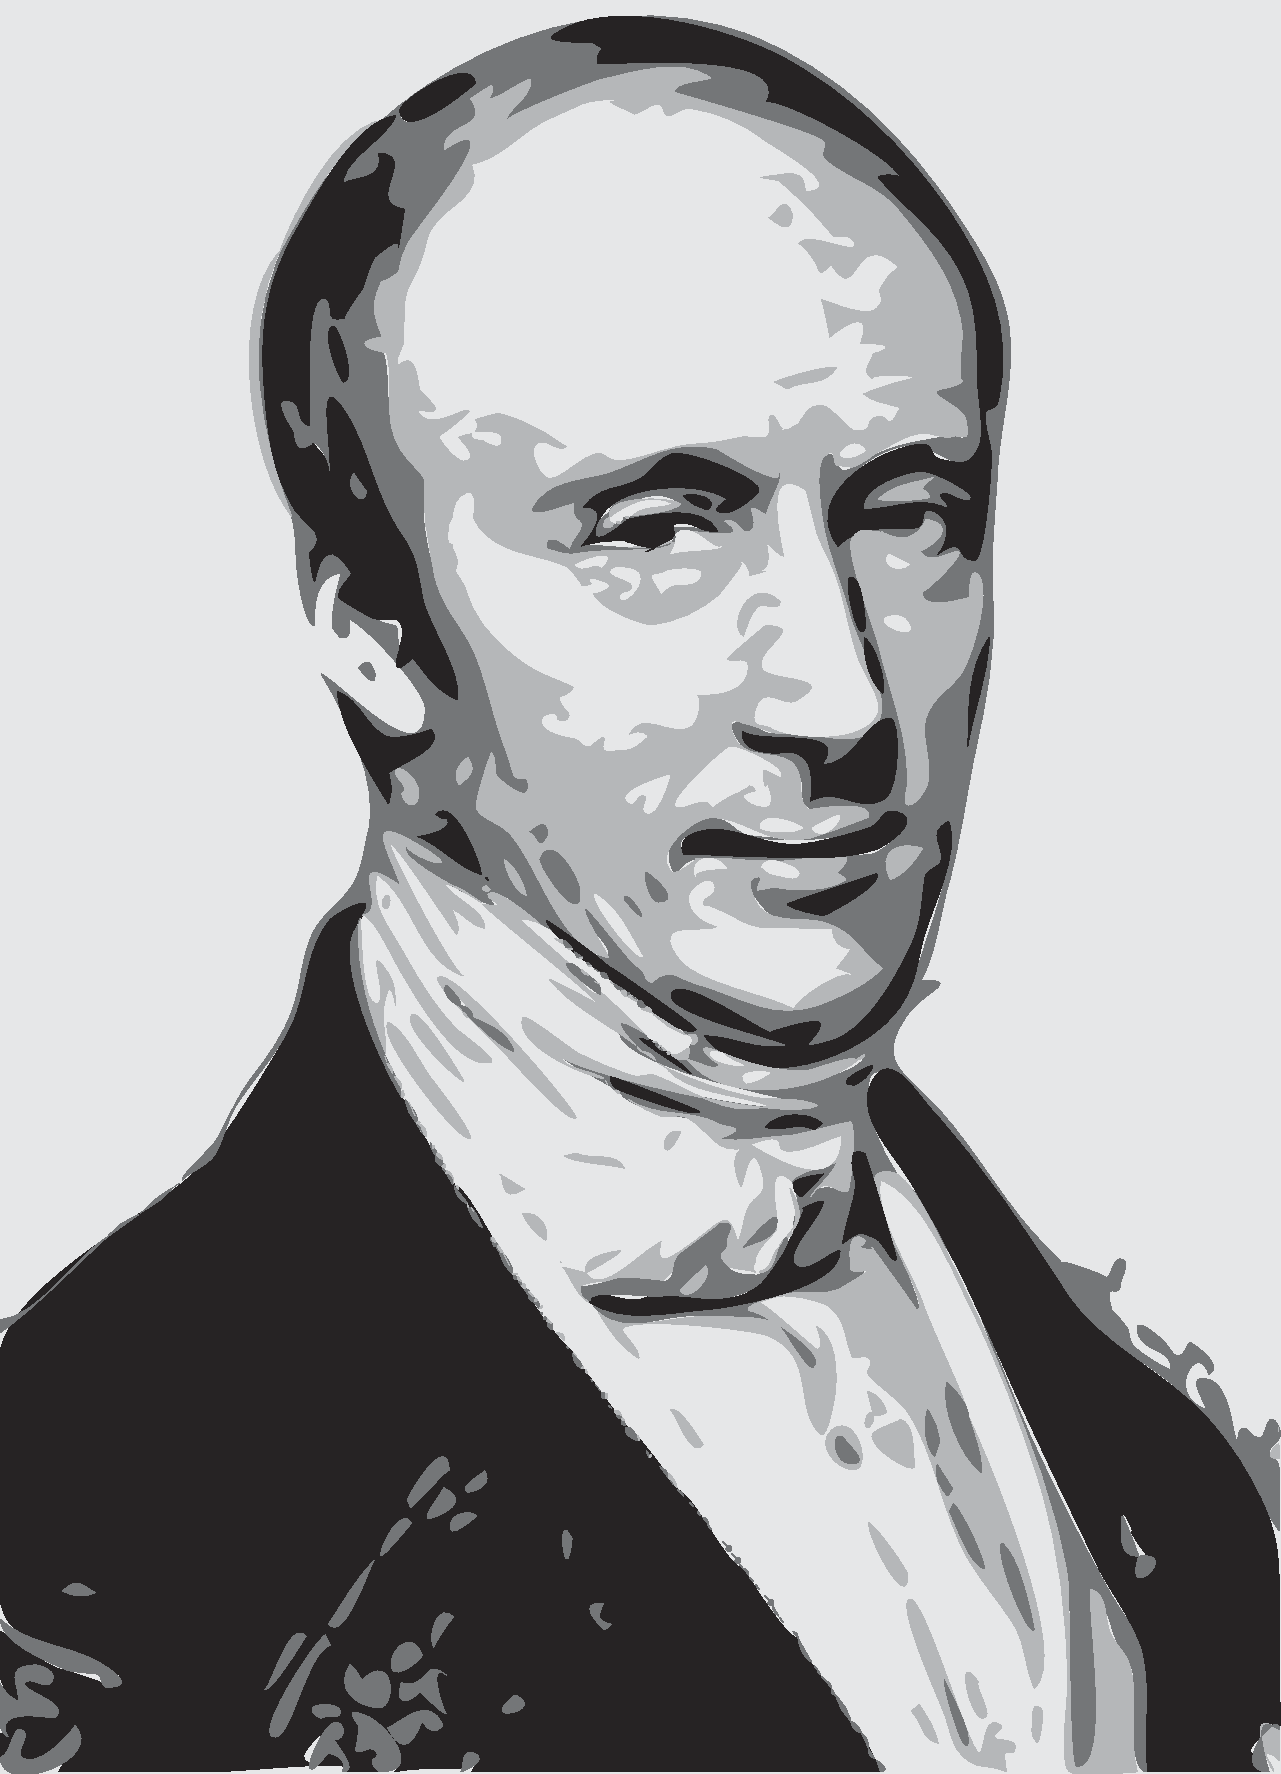
\includegraphics[width=.3\textwidth]{./fotos/calcasdos/Augustin-Louis_Cauchy.pdf}\\[5pt]  
  {\small\bfseries Augustin Cauchy}
\end{bio}

\begin{proposition}
  \label{convcau}Toda sucesión convergente en $X$ es de Cauchy.
\end{proposition}

\begin{proof}
  Si $x_{k}\rightarrow x$ en $X$ entonces, dada $\varepsilon >0$
  existe $k_{0}\in \mathbb{N}$ tal que
  $d_{X}(x_{k},x)<\frac{\varepsilon }{2}$ si $k\geq k_{0}$. Por tanto
  \begin{equation*}
    d_{X}(x_{k},x_{j})\leq d_{X}(x_{k},x)+d_{X}(x,x_{j})<\varepsilon \text{\qquad }\forall k,j\geq k_{0}.
  \end{equation*}
  Es decir, $(x_{k})$ es de Cauchy.
\end{proof}

No es cierto, en general, que cualquier sucesión de Cauchy
converge.  Veamos un par de ejemplos.

\begin{example}
  Sea $X:=(0,1)$ con la métrica inducida por la de
  $\mathbb{R}$. La sucesión $(\frac{1}{k})$ es de Cauchy en $X$
  pero no converge en $X$ \emph{[Ejercicio~\ref{ejnocompl}]}.
\end{example}

\begin{example}
  \label{C1nocompl}La sucesión de funciones
  $f_{k}\colon [-1,1]\rightarrow \mathbb{R}$,
  \begin{equation*}
    f_{k}(x)=
      \begin{cases}
        -1 & \text{si $-1\leq x\leq -\frac{1}{k}$,} \\ 
        kx & \text{si $-\frac{1}{k}\leq x\leq \frac{1}{k}$,} \\ 
        1 & \text{si $\frac{1}{k}\leq x\leq 1$,}
      \end{cases}
  \end{equation*}
  es de Cauchy en $\mathcal{C}_{1}^{0}[-1,1]$ pero no converge en
  $\mathcal{C}_{1}^{0}[-1,1]$.
\begin{figure}[htb]
  \centering
  \begin{tikzpicture}[scale=1.7]
  \draw (-1,0)--(1,0);
  \draw (0,-1)--(0,1);
  \draw[very thick] (-1,-1)--(-.333,-1)--(.333,1)--(1,1);
  \foreach \x in {-0.5, 0.5, -1, 1}{
               \draw[thin] (-.025,\x)--(0.025,\x);
};
  \foreach \x in {-1, 1}{
               \draw[thin] (\x,-0.025)--(\x,0.025);
};

\draw[dashed] (-.333,0) -- (-.333,-1);
\draw[dashed] (.333,0) -- (.333,1);
\draw (0,-1.2) node[below] {$y=f_k(x)$};

\draw (.333,-.025) node[below] {$\frac{1}{k}$};
\draw (1,-.025) node[below] {$1$};
\draw (-.333,.025) node[above] {$-\frac{1}{k}$};
\draw (-1,-.025) node[below] {$-1$};
%\draw (-.025,.5) node[left] {$\frac{1}{2}$};
\draw (-.025,1) node[left] {$1$};
%\draw (.025,-.5) node[right] {$-\frac{1}{2}$};
\draw (.025,-1) node[right] {$-1$};
\end{tikzpicture}

  % \caption{}\label{fig:1.1}
\end{figure}
\end{example}

\begin{proof}
  Para $j\geq k$ se tiene que
  \begin{equation*}
    \int_{-1}^{1}\left\vert f_{j}(x)-f_{k}(x)\right\vert dx=2\int_{0}^{1}\left(
      f_{j}(x)-f_{k}(x)\right) dx=\tfrac{1}{k}-\tfrac{1}{j}.
  \end{equation*}
  En consecuencia, dada $\varepsilon >0$ se cumple que
  \begin{equation*}
    \left\Vert f_{j}-f_{k}\right\Vert_{1}<\varepsilon \text{\qquad }\forall k,j>\tfrac{2}{\varepsilon }.
  \end{equation*}
  Así pues, $(f_{k})$ es de Cauchy.

  Argumentando por contradicción, supongamos que $f_{k}\rightarrow
  f$ en $\mathcal{C}_{1}^{0}[-1,1]$. Sea $a\in (0,1)$. Si $k\geq
  \frac{1}{a}$, entonces $f_{k}(x)=1$ para todo $x\in [a,1]$.
  En consecuencia,
  \begin{equation*}
    0\leq \int_{a}^{1}\left\vert 1-f(x)\right\vert dx\leq
    \int_{-1}^{1}\left\vert f_{k}(x)-f(x)\right\vert dx=\left\Vert
      f_{k}-f\right\Vert_{1}\rightarrow 0.
  \end{equation*}
  Por tanto,
  \begin{equation*}
    \int_{a}^{1}\left\vert 1-f(x)\right\vert dx=0,
  \end{equation*}
  lo que implica que $f(x)=1$ para todo $x\in [a,1]$.
  Análogamente, $f(x)=-1$ para todo $x\in [-1,-a]$ y, como
  $a\in (0,1)$ es arbitraria, tenemos que
  \begin{equation*}
    f(x)=
      \begin{cases}
        -1 & \text{si $x\in [-1,0)$,} \\ 
        1 & \text{si $x\in (0,1]$.}
      \end{cases}
  \end{equation*}
  En consecuencia, $f$ no es continua en $[-1,1]$, lo cual contradice
  nuestra suposición.
\end{proof}

En la siguiente sección probaremos que en $\mathcal{C}_{\infty
}^{0}[-1,1]$ cualquier sucesión de Cauchy converge. A los espacios
métricos que tienen esta propiedad se les llama completos.

\begin{definition}
  Un espacio métrico $X$ es \textbf{completo},
  \index{espacio!completo}si toda sucesión de Cauchy en $X$
  converge en $X$. Un espacio normado que es completo con la
  métrica inducida por su norma se llama un \textbf{espacio de
    Banach}.  \index{espacio!de Banach}
\end{definition}

Los ejemplos anteriores muestran que $(a,b)$ y
$\mathcal{C}_{1}^{0}[a,b]$ no son completos. De hecho,
$\mathcal{C}_{p}^{0}[a,b]$ no es un espacio de Banach para ninguna
$p\in [1,\infty )$ [Ejercicio~\ref{ejCpnocompl}].

La completitud no es invariante bajo homeomorfismos, como lo muestra
el siguiente ejemplo.

\begin{example}
  La función \ $\tan \colon (-\frac{\pi }{2},\frac{\pi }{2})\rightarrow
  \mathbb{R}$ \ es un homeomorfismo.  \ $\mathbb{R}$ es un espacio
  métrico completo, pero $(-\frac{\pi }{2},\frac{\pi }{2})$ no lo
  es.
\begin{figure}[htb]
  \centering
  \begin{tikzpicture}[domain=-6:6,scale=.6]
  \pgfmathsetmacro{\mypi}{3.14159}
  \draw[-latex'] (-6,0) -- (6,0);
  \draw[-latex'] (0,-2) -- (0,2);
  \draw[very thick] plot[samples=100](\x, {rad(atan(\x))});
  \draw[very thin,dashed] (-6,{\mypi/2}) -- (6,{\mypi/2});
  \draw[very thin,dashed] (-6,{-\mypi/2}) -- (6,{-\mypi/2});

  \draw (0,-2.2) node[below] {$y=\tan^{-1}(x)$};

\end{tikzpicture}
  % \caption{}\label{fig:5.2}
\end{figure}
\end{example}

Sin embargo, la completitud sí se preserva bajo equivalencias.

\begin{proposition}
  \label{equivcomplet}Si existe una equivalencia $\phi \colon X\rightarrow
  Y$ entre dos espacios métricos $X$ y $Y$, entonces $X$ es
  completo si y sólo si $Y$ lo es.
\end{proposition}

\begin{proof}
  Supongamos que $Y$ es completo y que $\phi \colon X\rightarrow Y$ es
  Lipschitz continua. Sea $(x_{k})$ una sucesión de Cauchy en
  $X$. Entonces, dada $\varepsilon >0$, existe $k_{0}\in \mathbb{N}$
  tal que
  \begin{equation*}
    d_{Y}(\phi (x_{j}),\phi (x_{k}))\leq c\,d_{X}(x_{j},x_{k})<\varepsilon \text{\qquad }\forall j,k\geq k_{0}.
  \end{equation*}
  Es decir, la sucesión $(\phi (x_{k}))$ es de Cauchy en $Y$ y, como
  $Y$ es completo, se tiene que $\phi (x_{k})\rightarrow y$ en
  $Y$. Ahora bien, como $\phi^{-1}$ es continua, la
  Proposición~\ref{contsuc} garantiza que
  $x_{k}=\phi^{-1}(\phi (x_{k}))\rightarrow \phi^{-1}(y)$ \ en
  $X$. Esto prueba que $X$ es completo. El recíproco se obtiene
  reemplazando $Y$ por $X$ y $\phi $ por $\phi^{-1}$ en el argumento
  anterior.
\end{proof}

Una consecuencia importante es la siguiente.

\begin{theorem}
  Todo espacio normado de dimensión finita es de Banach.
\end{theorem}

\begin{proof}
  Como para cualquier espacio normado $V$ de dimensión $n$ existe una
  equivalencia $\phi \colon \mathbb{R}_{\infty }^{n}\rightarrow V$
  (ver Ejercicio~\ref{ejnorfinequiv}), en virtud de la
  Proposición~\ref{equivcomplet} bastará probar que
  $\mathbb{R}_{\infty }^{n}$ es completo.

  Sea $(x_{k})$ una sucesión de Cauchy en $\mathbb{R}_{\infty
  }^{n}$, donde $x_{k}=(x_{k,1},\dots,x_{k,n})$. Entonces, dada
  $\varepsilon >0$, existe $k_{0}\in \mathbb{N}$ tal que
  \begin{equation*}
    \left\vert x_{j,i}-x_{k,i}\right\vert \leq \max_{i=1,\dots,n}\left\vert
      x_{j,i}-x_{k,i}\right\vert =\left\Vert x_{j}-x_{k}\right\Vert_{\infty
    }<\varepsilon\:\:\: \forall j,k\geq k_{0},\:
    \forall i=1,\dots,n.
  \end{equation*}
  Esto prueba que, para cada $i=1,\dots,n$, la sucesión $(x_{k,i})$
  es de Cauchy en $\mathbb{R}$. Como $\mathbb{R}$ es completo,
  $x_{k,i}\rightarrow x_{i}$ en $\mathbb{R}$. Por tanto, dada
  $\varepsilon >0$, existe $k_{i}\in \mathbb{N}$ tal que
  \begin{equation*}
    \left\vert x_{k,i}-x_{i}\right\vert <\varepsilon \text{\qquad }\forall k\geq
    k_{i},\text{ \ }\forall i=1,\dots,n,
  \end{equation*}
  y, en consecuencia,
  \begin{equation*}
    \left\Vert x_{k}-x\right\Vert_{\infty }=\max_{i=1,\dots,n}\left\vert
      x_{k,i}-x_{i}\right\vert <\varepsilon \text{\qquad }\forall k\geq \max
    \left\{k_{1},\dots,k_{n}\right\},
  \end{equation*}
  donde $x:=(x_{1},\dots,x_{n})$. Es decir, $x_{k}\rightarrow x$ en
  $\mathbb{R}_{\infty }^{n}$.
\end{proof}

No todo subespacio de un espacio métrico completo es un espacio
métrico completo. Por ejemplo, $\mathbb{R}$ es completo pero
ningún intervalo abierto $(a,b)$ lo es. La siguiente
proposición caracteriza a aquéllos que sí lo son.

\begin{proposition}
  \label{complcerr}Sea $X$ un espacio métrico completo. Un
  subespacio métrico $A$ de $X$ es completo si y sólo si es
  cerrado en $X$.
\end{proposition}

\begin{proof}
  $\Leftarrow )$: \ Supongamos que $A$ es cerrado en $X$. Sea
  $(a_{k})$ una sucesión de Cauchy en $A$. Entonces $(a_{k})$ es
  una sucesión de Cauchy en $X$ y, como $X$ es completo,
  $a_{k}\rightarrow x$ en $X$. Por la Proposición~\ref{cerrsuc} se
  tiene que $x\in \overline{A}=A$. Esto prueba que $A$ es completo.

  $\Rightarrow )$: \ Supongamos ahora que $A$ es completo. Sea
  $x\in \overline{A}$. Por la Proposición~\ref{cerrsuc}, existe una
  sucesión $(a_{k})$ en $A$ tal que $a_{k}\rightarrow x$ en $X$.  La
  Proposición~\ref{convcau} asegura entonces que $(a_{k})$ es de
  Cauchy y, como $A$ es completo, se tiene que $a_{k}\rightarrow a$ en
  $A$. De la unicidad del límite (ver Proposición~\ref{unilim}) se
  sigue que $x=a\in A$. En consecuencia, $A$ es cerrado.
\end{proof}

\section{Convergencia uniforme}

En esta sección daremos ejemplos importantes de espacios
métricos completos. Empezaremos comparando ciertos tipos de
convergencia para sucesiones de funciones.

Sean $S$ un conjunto y $X=(X,d_{X})$ un espacio métrico.

\begin{definition}
  Una sucesión de funciones $f_{k}\colon S\rightarrow X$, $k\in
  \mathbb{N}$, converge \textbf{puntualmente}
  \index{convergencia!puntual}en $S$ a una función $f\colon S\rightarrow
  X$ si $f_{k}(z)\rightarrow f(z)$ en $X$ para cada $z\in S$. Es
  decir, si para cada $\varepsilon >0$ y cada $z\in S$ existe
  $k_{0}\in \mathbb{N}$ (que depende de $\varepsilon $ y de $z)$ tal
  que
  \begin{equation*}
    d_{X}(f_{k}(z),f(z))<\varepsilon 
    \text{\qquad }\forall k\geq k_{0}.
  \end{equation*}
  La función $f$ se llama el \textbf{límite puntual}
  \index{limite@límite!puntual}de $(f_{k})$.
\end{definition}

El límite puntual de una sucesión de funciones continuas no
es, por lo general, una función continua, como lo muestra el
siguiente ejemplo.

\begin{example}
  \label{limpun}La sucesión de funciones $f_{k}\colon [0,1]\rightarrow
  \mathbb{R}$, $f_{k}(x)=x^{k}$, converge puntualmente a
  \begin{equation*}
    f(x)=
      \begin{cases}
        0 & 
        \text{si $0\leq x<1$,} \\ 
        1 & \text{si $x=1$.}
      \end{cases}
  \end{equation*}
\begin{figure}[htb]
  \centering
  \begin{tikzpicture}[scale=2]
  \draw (0,0)--(1,0);
  \draw (0,0)--(0,1);

  \draw[very thick] plot[samples=100, domain=0:1](\x, {(\x)^2});
  \draw (0.5,-0.3) node[below] {$y=x^2$};
  
  \foreach \x in {0.5, 1}{
               \draw[thin] (\x,-0.025)--(\x,0.025);
               \draw[thin] (-.025,\x)--(0.025,\x);
};
  \draw (0,-.025) node[below] {$0$};
%  \draw (.5,-.025) node[below] {$\frac{1}{2}$};
  \draw (1,-.025) node[below] {$1$};
%  \draw (-.025,.5) node[left] {$\frac{1}{2}$};
  \draw (-.025,1) node[left] {$1$};
\end{tikzpicture}
\qquad\qquad 
  \begin{tikzpicture}[scale=2]
  \draw (0,0)--(1,0);
  \draw (0,0)--(0,1);

  \draw[very thick] plot[samples=100, domain=0:1](\x, {(\x)^4});
  \draw (0.5,-0.3) node[below] {$y=x^4$};
  
  \foreach \x in {0.5, 1}{
               \draw[thin] (\x,-0.025)--(\x,0.025);
               \draw[thin] (-.025,\x)--(0.025,\x);
};
  \draw (0,-.025) node[below] {$0$};
%  \draw (.5,-.025) node[below] {$\frac{1}{2}$};
  \draw (1,-.025) node[below] {$1$};
%  \draw (-.025,.5) node[left] {$\frac{1}{2}$};
  \draw (-.025,1) node[left] {$1$};
\end{tikzpicture}
\qquad\qquad
  \begin{tikzpicture}[scale=2]
  \draw (0,0)--(1,0);
  \draw (0,0)--(0,1);

  \draw[very thick] plot[samples=100, domain=0:1](\x, {(\x)^6});
  \draw (0.5,-0.3) node[below] {$y=x^6$};
  
  \foreach \x in {0.5, 1}{
               \draw[thin] (\x,-0.025)--(\x,0.025);
               \draw[thin] (-.025,\x)--(0.025,\x);
};
  \draw (0,-.025) node[below] {$0$};
%  \draw (.5,-.025) node[below] {$\frac{1}{2}$};
  \draw (1,-.025) node[below] {$1$};
%  \draw (-.025,.5) node[left] {$\frac{1}{2}$};
  \draw (-.025,1) node[left] {$1$};
\end{tikzpicture}

  % \caption{}\label{fig:5.4}
\end{figure}
\end{example}

Daremos a continuación una noción de convergencia según la
cual el límite de una sucesión de funciones continuas
resultará ser una función continua.

\begin{definition}
  Una sucesión de funciones $f_{k}\colon S\rightarrow X$, $k\in
  \mathbb{N}$, converge \textbf{uniformemente}
  \index{convergencia!uniforme}en $S$ a una función
  $f\colon S\rightarrow X$ si, dada $\varepsilon >0$, existe $k_{0}\in
  \mathbb{N}$ (que depende de $\varepsilon )$ tal que
  \begin{equation*}
    d_{X}(f_{k}(z),f(z))<\varepsilon 
    \text{\qquad }\forall k\geq k_{0}\text{, \ }\forall z\in S.
  \end{equation*}
  La función $f$ se llama el \textbf{límite uniforme}
  \index{limite@límite!uniforme}de $(f_{k})$.
\end{definition}

Nota que esta noción es más fuerte que la de convergencia
puntual: si $(f_{k})$ converge uniformemente a $f$, entonces converge
puntualmente a $f$. El recíproco no es cierto pues la
sucesión $(f_{k})$ del Ejemplo~\ref{limpun} no converge
uniformemente en $[0,1]$ \ [Ejercicio~\ref{ejnoconvuni}]. El siguiente
ejemplo muestra que, aun cuando una sucesión de funciones
continuas converge puntualmente a una función continua, no
necesariamente converge uniformemente.

\begin{example}
  \label{puntnounif}Sea $f_{k}\colon [0,1]\rightarrow \mathbb{R}$ la
  función dada por
  \begin{equation*}
    f_{k}(x)=\max \left\{1-k\left\vert x-\tfrac{1}{k}\right\vert ,0\right\} .
  \end{equation*}
\begin{figure}[htb]
  \centering
  \begin{tikzpicture}[scale=2]
  \draw (0,0)--(1,0);
  \draw (0,0)--(0,1);

  \draw[very thick] (0,0)--(.25,1)--(.5,0)--(1,0);
  \draw (0.5,-0.35) node[below] {$y=f_k(x)$};
  
  \foreach \x in {0.5, 1}{
               \draw[thin] (\x,-0.025)--(\x,0.025);
               \draw[thin] (-.025,\x)--(0.025,\x);
};
\draw[dashed] (.25,0) -- (.25,1);
  \draw (0,-.025) node[below] {$0$};
  \draw (.25,-.025) node[below] {$\frac{1}{k}$};
  \draw (.5,-.025) node[below] {$\frac{2}{k}$};
  \draw (1,-.025) node[below] {$1$};
%  \draw (-.025,.5) node[left] {$\frac{1}{2}$};
  \draw (-.025,1) node[left] {$1$};
\end{tikzpicture}

  % \caption{}\label{fig:5.5}
\end{figure}
  La sucesión $(f_{k})$ converge puntualmente a $0$, pero no
  converge uniformemente a $0$ ya que, si $\varepsilon \in (0,1)$,
  ningún $k\in \mathbb{N}$ cumple que $\left\vert
    f_{k}(x)\right\vert <\varepsilon $ para todo $x\in [0,1]$.
  En efecto:
  \begin{equation*}
    \left\vert f_{k}\left(\tfrac{1}{k}\right) \right\vert =1>\varepsilon \text{\qquad }\forall k\in \mathbb{N}.
  \end{equation*}
\end{example}

La propiedad fundamental de la convergencia uniforme es la siguiente.

\begin{theorem}
  \label{contlimuni}Sean $Z=(Z,d_{Z})$ y $X=(X,d_{X})$ espacios
  métricos.  Si $f_{k}\colon Z\rightarrow X$ es continua para todo $k\in
  \mathbb{N}$ y $(f_{k})$ converge uniformemente a $f$ en $Z$,
  entonces $f\colon Z\rightarrow X$ es continua.
\end{theorem}

\begin{proof}
  Sean $z_{0}\in Z$ y $\varepsilon >0$. Como $(f_{k})$ converge
  uniformemente a $f$, existe $k_{0}\in \mathbb{N}$ tal que
  \begin{equation*}
    d_{X}(f_{k}(z),f(z))<\frac{\varepsilon }{3}\text{\qquad }\forall z\in Z,\text{ \ }\forall k\geq k_{0}.
  \end{equation*}
  Y, como $f_{k_{0}}$ es continua, existe $\delta >0$ tal que
  \begin{equation*}
    d_{X}(f_{k_{0}}(z),f_{k_{0}}(z_{0}))<\frac{\varepsilon }{3}\text{\qquad si \ 
    }d_{Z}(z,z_{0})<\delta .
  \end{equation*}
  En consecuencia,
  \begin{align*}
    d_{X}(f(z),f(z_{0})) &\leq
    d_{X}(f(z),f_{k_{0}}(z))+d_{X}(f_{k_{0}}(z),f_{k_{0}}(z_{0}))+d_{X}(f_{k_{0}}(z_{0}),f(z_{0}))
    \\
    &<\varepsilon \text{\qquad si \ }d_{Z}(z,z_{0})<\delta .
  \end{align*}
  Esto prueba que $f$ es continua.
\end{proof}

Para funciones acotadas la convergencia uniforme es simplemente la
convergencia en el espacio métrico $\mathcal{B}(S,X)$, definido en
la Sección~\ref{espfuncacot}, cuya métrica es la métrica
uniforme
\begin{equation*}
  d_{\infty }(f,g)=\sup_{z\in S}d_{X}(f(z),g(z)),\text{\qquad }f,g\in \mathcal{B}(S,X).
\end{equation*}
Es decir, se tiene el siguiente resultado.

{\abovedisplayskip=8pt%
  \belowdisplayskip=9pt%
\begin{proposition}
  \label{convB=cu}Sea $(f_{k})$ una sucesión en
  $\mathcal{B}(S,X)$. Entonces, $(f_{k})$ converge uniformemente a $f$
  en $S$ si y sólo si $(f_{k})$ converge a $f$\ en
  $\mathcal{B}(S,X)$.
\end{proposition}

\begin{proof}
  $\Leftarrow )$: \ Si $(f_{k})$ converge a $f$\ en $\mathcal{B}(S,X)$
  entonces, dada $\varepsilon >0$, existe $k_{0}\in \mathbb{N}$ tal
  que
  \begin{equation*}
    d_{\infty }(f_{k},f)=\sup_{z\in S}d_{X}(f_{k}(z),f(z))<\varepsilon \text{\qquad }\forall k\geq k_{0}.
  \end{equation*}
  En consecuencia,
  \begin{equation*}
    d_{X}(f_{k}(z),f(z))<\varepsilon \text{\qquad }\forall k\geq k_{0},\text{ \ }\forall z\in S.
  \end{equation*}
  Es decir, $(f_{k})$ converge uniformemente a $f$ en $S$.

  $\Rightarrow )$: \ Recíprocamente, si $f_{k}\in
  \mathcal{B}(S,X)$ y $(f_{k})$ converge uniformemente a $f$ en $S$
  entonces, dada $\varepsilon >0$, existe $k_{0}\in N$ tal que
  \begin{equation}
    d_{X}(f_{k}(z),f(z))<\varepsilon \text{\qquad }\forall k\geq k_{0},\text{ \ }\forall z\in S.  \label{cu}
  \end{equation}
  Como $f_{k_{0}}$ es acotada, existen $c>0$ y $x_{0}\in X$ tales que
  $d_{X}(f_{k_{0}}(z),x_{0})<c$ para todo $z\in S$. En consecuencia,
  \begin{equation*}
    d_{X}(f(z),x_{0})\leq
    d_{X}(f(z),f_{k_{0}}(z))+d_{X}(f_{k_{0}}(z),x_{0})<\varepsilon +c\text{\qquad }\forall z\in S.
  \end{equation*}
  Esto prueba que $f\in \mathcal{B}(S,X)$. De (\ref{cu}) se sigue que
  \begin{equation*}
    d_{\infty }(f_{k},f)=\sup_{z\in S}d_{X}(f_{k}(z),f(z))\leq \varepsilon \text{\qquad }\forall k\geq k_{0}.
  \end{equation*}
  Es decir, $(f_{k})$ converge a $f$\ en $\mathcal{B}(S,X)$.
\end{proof}

El siguiente espacio jugará un papel importante en las
aplicaciones del próximo capítulo.

\begin{definition}
  \label{defespfuncont}Sean $Z$ y $X$ espacios métricos. El
  \textbf{espacio de funciones continuas y acotadas} 
\index{espacio!C subb0ZX@$\mathcal{C}_{b}^{0}(Z,X)\vspaceindex$}de $Z$ a
  $X$ es el espacio métrico
  \begin{equation*}
    \mathcal{C}_{b}^{0}(Z,X):=\left\{f\colon Z\rightarrow X:f\text{ es continua y acotada}\right\}
  \end{equation*}
  con la métrica inducida por la de $\mathcal{B}(Z,X)$, es decir,
  \begin{equation*}
    d_{\infty }(f,g)=\sup_{z\in Z}d_{X}(f(z),g(z))
  \end{equation*}
  si $f,g\in \mathcal{C}_{b}^{0}(Z,X)$.
\end{definition}
}

Para sucesiones de funciones continuas y acotadas podemos
reinterpretar el Teorema~\ref{contlimuni} como sigue.

\begin{corollary}
  \label{contcerrenacot}Sean $Z$ y $X$ espacios métricos. Entonces
  $\mathcal{C}_{b}^{0}(Z,X)$ es un subespacio cerrado de
  $\mathcal{B}(Z,X)$.
\end{corollary}

\begin{proof}
  Sea $f\in \overline{\mathcal{C}_{b}^{0}(Z,X)}$. Por la
  Proposición~\ref{cerrsuc} existe una sucesión $(f_{k})$ en
  $\mathcal{C}_{b}^{0}(Z,X)$ tal que $f_{k}\rightarrow f$ en
  $\mathcal{B}(Z,X)$. La Proposición~\ref{convB=cu} y el
  Teorema~\ref{contlimuni} aseguran entonces que
  $f\in \mathcal{C}_{b}^{0}(Z,X)$. Esto prueba que
  $\mathcal{C}_{b}^{0}(Z,X)$ es cerrado en $\mathcal{B}(Z,X)$.
\end{proof}

Concluimos esta sección con otra consecuencia importante de la
convergencia uniforme.

\begin{theorem}
  \label{limunifdif}Si $f_{k}\colon [a,b]\rightarrow \mathbb{R}$ es una
  sucesión de funciones continuamente diferenciables en $[a,b]$
  tales que $(f_{k})$ converge a $f$ puntualmente en $[a,b]$ y
  $(f_{k}^{\prime })$ converge a $g$ uniformemente en $[a,b]$,
  entonces $f$ es continuamente diferenciable en $[a,b]$ y $f^{\prime
  }=g$.
\end{theorem}

\begin{proof}
  Sea $x_{0}\in (a,b)$. Aplicando el teorema del valor medio a la
  función $f_{j}-f_{k}$\ se tiene que, para cada $x\in (a,b)$,
  existe $\xi_{x}\in (a,b) $ tal que
  \begin{equation*}
    f_{j}(x)-f_{k}(x)-(f_{j}(x_{0})-f_{k}(x_{0}))=\left( f_{j}^{\prime }(\xi
     _{x})-f_{k}^{\prime }(\xi_{x})\right) (x-x_{0}).
  \end{equation*}
  En consecuencia,
  \begin{equation*}
    \left\vert f_{j}(x)-f_{j}(x_{0})-f_{k}(x)+f_{k}(x_{0})\right\vert \leq
    \left\Vert f_{j}^{\prime }-f_{k}^{\prime }\right\Vert_{\infty }\left\vert
      x-x_{0}\right\vert \text{\qquad }\forall x\in (a,b).
  \end{equation*}
  Como $(f_{k}^{\prime })$ converge en $\mathcal{C}^{0}[a,b]$, dada
  $\varepsilon >0$\ existe $k_{0}\in \mathbb{N}$\ tal que
  \begin{equation*}
    \left\vert f_{j}(x)-f_{j}(x_{0})-f_{k}(x)+f_{k}(x_{0})\right\vert \leq \frac{\varepsilon }{3}\left\vert x-x_{0}\right\vert \qquad \forall x\in (a,b),\text{ \ }\forall j,k\geq k_{0}.
  \end{equation*}
  Tomando el límite cuando $j\rightarrow \infty $,\ concluimos
  que
  \begin{equation}
    \left\vert f(x)-f(x_{0})-f_{k}(x)+f_{k}(x_{0})\right\vert \leq \frac{\varepsilon }{3}\left\vert x-x_{0}\right\vert \qquad \forall x\in (a,b),\text{ \ }\forall k\geq k_{0}.  \label{uno}
  \end{equation}
  Por otra parte, existe $k_{1}\in \mathbb{N}$\ tal que
  \begin{equation}
    \left\vert f_{k}^{\prime }(x_{0})-g(x_{0})\right\vert <\frac{\varepsilon }{3}\qquad \forall k\geq k_{1}.  \label{dos}
  \end{equation}
  Sea $k_{\ast }:=\max \left\{k_{0},k_{1}\right\}$, y sea $\delta >0$ tal que
  \begin{equation}
    \left\vert \frac{f_{k_{\ast }}(x)-f_{k_{\ast }}(x_{0})}{x-x_{0}}-f_{k_{\ast
        }}^{\prime }(x_{0})\right\vert <\frac{\varepsilon }{3}\qquad \text{si }\left\vert x-x_{0}\right\vert <\delta .  \label{tres}
  \end{equation}
  De las desigualdades (\ref{uno}), (\ref{dos}) y (\ref{tres}) se
  sigue que
  \begin{align*}
    \left\vert \frac{f(x)-f(x_{0})}{x-x_{0}}-g(x_{0})\right\vert &\leq
    \left\vert \frac{f(x)-f(x_{0})}{x-x_{0}}-\frac{f_{k_{\ast }}(x)-f_{k_{\ast
          }}(x_{0})}{x-x_{0}}\right\vert \\
    &\qquad{}+\left\vert \frac{f_{k_{\ast }}(x)-f_{k_{\ast }}(x_{0})}{x-x_{0}}-f_{k_{\ast }}^{\prime }(x_{0})\right\vert +\left\vert f_{k_{\ast }}^{\prime
      }(x_{0})-g(x_{0})\right\vert \\
    &<\varepsilon \qquad \text{si \ }\left\vert x-x_{0}\right\vert <\delta .
  \end{align*}
  Es decir, $f\ $es diferenciable en $x_{0}$ y $f^{\prime
  }(x_{0})=g(x_{0})$. Finalmente, como $f_{k}^{\prime }\in
  \mathcal{C}^{0}[a,b]$, se tiene que $g\in \mathcal{C}^{0}[a,b]$, es
  decir, $f$ es continuamente diferenciable en $[a,b]$.
\end{proof}

\section{Espacios completos de funciones}

A continuación daremos un criterio que garantiza la convergencia
uniforme de una sucesión de funciones en términos de la
sucesión misma.

Sean $S$ un conjunto y $X=(X,d_{X})$ un espacio métrico.

{\abovedisplayskip=7pt%
\belowdisplayskip=8pt%
\begin{definition}
  Una sucesión de funciones $f_{k}\colon S\rightarrow X$, $k\in
  \mathbb{N}$, es \textbf{uniformemente de Cauchy}
  \index{sucesión!uniformemente de Cauchy}en $S$ si, para cada
  $\varepsilon >0$, existe $k_{0}\in \mathbb{N}$ tal que
  \begin{equation*}
    d_{X}(f_{k}(z),f_{j}(z))<\varepsilon \qquad \forall j,k\geq k_{0}\text{, \ }\forall z\in S.
  \end{equation*}
\end{definition}

El siguiente teorema nos da una condición necesaria y suficiente
para la convergencia uniforme de una sucesión de funciones.

\begin{theorem}[Criterio de convergencia uniforme de Cauchy]
  \label{cricau}\index{criterio!de convergencia uniforme}Sea $X$ un
  espacio métrico completo. Una sucesión de funciones
  $f_{k}\colon S\rightarrow X$, $k\in \mathbb{N}$, converge uniformemente en
  $S$ si y sólo si $(f_{k})$ es uniformemente de Cauchy en $S$.
\end{theorem}

\begin{proof}
  $\Rightarrow )$: \ \textit{Si }$(f_{k})$ converge uniformemente a
  $f$ en $S$ entonces, dada $\varepsilon >0$, existe $k_{0}\in
  \mathbb{N}$ tal que
  \begin{equation*}
    d_{X}(f_{k}(z),f(z))<\frac{\varepsilon }{2}\qquad \forall k\geq k_{0}\text{, \ }\forall z\in S.
  \end{equation*}
  En consecuencia,
  \begin{equation*}
    d_{X}(f_{k}(z),f_{j}(z))\leq
    d_{X}(f_{k}(z),f(z))+d_{X}(f(z),f_{j}(z))<\varepsilon \qquad \forall j,k\geq
    k_{0}\text{, \ }\forall z\in S.
  \end{equation*}
  Es decir, $(f_{k})$ es uniformemente de Cauchy.

  $\Leftarrow )$: \ Supongamos ahora que $(f_{k})$ es uniformemente de
  Cauchy en $S$. Entonces, para cada $z\in S$, la sucesión
  $(f_{k}(z))$ es de Cauchy en $X$ y, como $X$ es completo, esta
  sucesión converge a un punto de $X$ al que denotaremos por
  $f(z)$. Probaremos ahora que $f_{k}\rightarrow f$ uniformemente en
  $S$.

  Sea $\varepsilon >0$. Como $(f_{k})$ es uniformemente de Cauchy,
  existe $k_{0}\in \mathbb{N}$ tal que
  \begin{equation*}
    d_{X}(f_{k}(z),f_{j}(z))<\frac{\varepsilon }{2}\qquad \forall j,k\geq k_{0}\text{, \ }\forall z\in S.
  \end{equation*}
  Y como para cada $z\in S$ se tiene que$\ f_{j}(z)\rightarrow f(z)$
  en $X$, existe $k(z)\in \mathbb{N}$ (que depende de $z$) tal que
  \begin{equation*}
    d_{X}(f_{j}(z),f(z))<\frac{\varepsilon }{2}\qquad \forall j\geq k(z)\text{.}
  \end{equation*}
  Dadas $k\geq k_{0}$ y $z\in S$, tomemos $j:=\max \left\{k_{0},k(z)\right\}$.
  Entonces
  \begin{equation*}
    d_{X}(f_{k}(z),f(z))\leq
    d_{X}(f_{k}(z),f_{j}(z))+d_{X}(f_{j}(z),f(z))<\varepsilon \text{.}
  \end{equation*}
  En consecuencia,
  \begin{equation*}
    d_{X}(f_{k}(z),f(z))<\varepsilon \qquad \forall k\geq k_{0}\text{, \ }\forall z\in S,
  \end{equation*}
  es decir, $(f_{k})$ converge uniformemente a $f$.
\end{proof}
}
Recuerda que, si $S$ es un conjunto y $V=(V,\left\Vert \cdot
\right\Vert )$ es un espacio vectorial normado, entonces
$\mathcal{B}(S,V)$ con la norma uniforme
\begin{equation}
  \left\Vert f\right\Vert_{\infty }=\sup_{z\in S}\left\Vert f(z)\right\Vert
  \label{normuni}
\end{equation}
es un espacio vectorial normado (ver Ejercicio~\ref{ejnormunif}). Si
$Z$ es un espacio métrico, $\mathcal{C}_{b}^{0}(Z,V)$ es un
subespacio vectorial de $\mathcal{B}(Z,V)$.

Una consecuencia importante del teorema anterior es la siguiente.

\begin{theorem}
  \label{funcacotcompl}Sean $S$ un conjunto y $Z$ un espacio
  métrico.

  \begin{itemize}
  \item Si $X$ es un espacio métrico completo, entonces
    $\mathcal{B}(S,X)$\ y\ $\mathcal{C}_{b}^{0}(Z,X)$ son completos.

  \item Si $V$ es un espacio de Banach, entonces $\mathcal{B}(S,V)$\
    y\ $\mathcal{C}_{b}^{0}(Z,V)$ son espacios de Banach.
  \end{itemize}
\end{theorem}

\begin{proof}
  Sea $(f_{k})$ una sucesión de Cauchy en $\mathcal{B}(S,X)$.
  Claramente $(f_{k})$ es uniformemente de Cauchy en $S$ y, por la
  Proposición~\ref{convB=cu} y el Teorema~\ref{cricau}, $(f_{k})$
  converge en $\mathcal{B}(S,X)$. Esto prueba que $\mathcal{B}(S,X)$
  es completo. Por el Corolario~\ref{contcerrenacot},
  $\mathcal{C}_{b}^{0}(Z,X)$ es un subconjunto cerrado de
  $\mathcal{B}(Z,X)$. La Proposición~\ref{complcerr} asegura
  entonces que $\mathcal{C}_{b}^{0}(Z,X)$ es completo.
\end{proof}

Esta propiedad permite que los espacios $\mathcal{B}(S,X)$ y
$\mathcal{C}_{b}^{0}(Z,X)$ jueguen un papel importante en las
aplicaciones, como veremos en el siguiente capítulo.

Recuerda que, si $K$ es un espacio métrico compacto, entonces toda
función continua de $K$ en $X$ es acotada (ver Corolario
\ref{contencomp}), es decir,
%\index{espacio!de funciones continuas@$\mathcal{C}^{0}(K,X)$}
\begin{equation*}
  \mathcal{C}^{0}(K,X):=\left\{\phi \colon K\rightarrow X:\phi 
  \text{ es continua}\right\}=\mathcal{C}_{b}^{0}(K,X).
\end{equation*}
Por tanto, $\mathcal{C}^{0}(K,X)$ es un espacio completo si $K$ es
compacto y $X$ es completo.

\section{Series en espacios de Banach}

Sea $V=(V,\left\Vert \cdot \right\Vert )$ un espacio vectorial normado
y sea $(v_{k})$ una sucesión en $V$.

\begin{definition}
  Decimos que \textbf{la serie }\index{serie}
  \begin{equation*}
    \sum_{k=1}^{\infty }v_{k}
  \end{equation*}
  \textbf{converge} \index{convergencia!de una serie}en $V$ si la
  sucesión $(w_{n})$ de sumas parciales
  $w_{n}:=\sum_{k=1}^{n}v_{k}$ converge en $V$. Su límite se
  denota
  \begin{equation*}
    \sum_{k=1}^{\infty }v_{k}:=\lim_{n\rightarrow \infty }\sum_{k=1}^{n}v_{k}.
  \end{equation*}
\end{definition}

Una observación sencilla es la siguiente.

\begin{proposition}
  \label{serconvacot}Si la serie $\sum_{k=1}^{\infty }v_{k}$ converge
  en $V$, entonces $v_{k}\rightarrow 0$ en $V$. En particular,
  $(v_{k})$ está acotada.
\end{proposition}

\begin{proof}
  La sucesión $(w_n)$, donde $w_n:=\sum_{k=1}^{n}v_{k}$, es de Cauchy
  (ver Proposición~\ref{convcau}). Por tanto, dada $\varepsilon
  >0$, existe $n_{0}\in \mathbb{N}$ tal que
  \begin{equation*}
    \left\Vert v_{n+1}\right\Vert =\left\Vert
      \sum_{k=1}^{n+1}v_{k}-\sum_{k=1}^{n}v_{k}\right\Vert \leq
    \varepsilon \qquad \forall n\geq n_{0}.
  \end{equation*}
  Esto prueba que $v_{k}\rightarrow 0$ en $V$. Por la
  Proposición~\ref{succonvacot}, $(v_{k})$ está acotada.
\end{proof}

En espacios de Banach se tiene el siguiente criterio de convergencia
para series.
\pagebreak
\begin{proposition}[Criterio de Cauchy para series]
  \label{critcauser}\index{criterio!de Cauchy para series}Sea $V$ un
  espacio de Banach y sea $(v_{k})$ una sucesión en $V$. La serie
  \begin{equation*}
    \sum_{k=1}^{\infty }v_{k}
  \end{equation*}
  converge en $V$ si y sólo si, para cada $\varepsilon >0$, existe
  $k_{0}\in \mathbb{N}$ tal que
  \begin{equation*}
    \left\Vert v_{k+1}+\cdots +v_{k+j}\right\Vert <\varepsilon \qquad \forall
    k\geq k_{0},\text{ \ }\forall j\geq 1.
  \end{equation*}
\end{proposition}

\begin{proof}
  Como $V$ es completo, la sucesión $(w_{n})$ de sumas parciales
  $w_{n}:=\sum_{k=1}^{n}v_{k}$ converge en $V$ si y sólo si
  $\left( w_{n}\right) $ es de Cauchy, es decir, si y sólo si para
  cada $\varepsilon >0$, existe $k_{0}\in N$ tal que
  \begin{equation*}
    \left\Vert w_{k+j}-w_{k}\right\Vert =\left\Vert v_{k+1}+\cdots
      +v_{k+j}\right\Vert <\varepsilon \qquad \forall k\geq k_{0},\text{ \ }\forall j\geq 1,
  \end{equation*}
  como afirma el enunciado.
\end{proof}

El siguiente criterio garantiza la convergencia uniforme de una serie
de funciones en términos de la convergencia de una serie de
números reales.

\begin{theorem}[Criterio de Weierstrass]
  \label{cw}\index{criterio!de Weierstrass para series}Sea $V$ un
  espacio de Banach y sea $(v_{k})$ una sucesión en $V$. Si la
  serie de números reales
  \begin{equation*}
    \sum_{k=1}^{\infty }\left\Vert v_{k}\right\Vert
  \end{equation*}
  \ converge, entonces la serie
  \begin{equation*}
    \sum_{k=1}^{\infty }v_{k}
  \end{equation*}
  converge en $V$ y se cumple que
  \begin{equation*}
    \left\Vert \sum_{k=1}^{\infty }v_{k}\right\Vert \leq \sum_{k=1}^{\infty
    }\left\Vert v_{k}\right\Vert .
  \end{equation*}
\end{theorem}

\begin{proof}
  Sea $\varepsilon >0$. Como
  $\sum_{k=1}^{\infty }\left\Vert v_{k}\right\Vert $ converge en
  $\mathbb{R}$, la Proposición~\ref{critcauser} asegura que existe
  $k_{0}\in \mathbb{N}$ tal que
  \begin{equation*}
    \left\Vert v_{k+1}\right\Vert +\cdots +\left\Vert v_{k+j}\right\Vert
    <\varepsilon \qquad \forall k\geq k_{0},\text{ \ }\forall j\geq 1.
  \end{equation*}
  Usando la desigualdad del triángulo obtenemos que
{\abovedisplayskip=9pt 
\belowdisplayskip=9pt%
  \begin{equation*}
    \left\Vert v_{k+1}+\cdots +v_{k+j}\right\Vert \leq \left\Vert
      v_{k+1}\right\Vert +\cdots +\left\Vert v_{k+j}\right\Vert <\varepsilon
    \qquad \forall k\geq k_{0},\text{ \ }\forall j\geq 1.
  \end{equation*}
  Aplicando nuevamente la Proposición~\ref{critcauser} concluimos
  que la serie
  \begin{equation*}
    \sum_{k=1}^{\infty }v_{k}
  \end{equation*}
  converge en $V$. En consecuencia, usando la continuidad de la norma
  y la desigualdad del triángulo obtenemos
  \begin{equation*}
    \left\Vert \sum_{k=1}^{\infty }v_{k}\right\Vert =\lim_{n\rightarrow \infty
    }\left\Vert \sum_{k=1}^{n}v_{k}\right\Vert \leq \lim_{n\rightarrow \infty
    }\sum_{k=1}^{n}\left\Vert v_{k}\right\Vert =\sum_{k=1}^{\infty }\left\Vert
      v_{k}\right\Vert ,
  \end{equation*}
  como afirma el enunciado.}
\end{proof}
{\abovedisplayskip=9pt% 
\belowdisplayskip=9pt%
Sea $S$ un conjunto y sea $f_{k}\colon S\rightarrow V$ una sucesión de
funciones.

\begin{definition}
  Decimos que \textbf{la serie de funciones }\index{serie!de
    funciones}\textbf{\ }
  \begin{equation*}
    \sum_{k=1}^{\infty }f_{k}
  \end{equation*}
  \textbf{converge uniformemente en} \index{convergencia!uniforme de
    una serie}$S$ si la sucesión de funciones
  $g_{n}:=\sum_{k=1}^{n}f_{k}$ converge uniformemente en $S$ a una
  función $S\rightarrow V$, a la que se denota
  \begin{equation*}
    \sum_{k=1}^{\infty }f_{k}.
  \end{equation*}
\end{definition}

Un ejemplo importante de series de funciones son las series de
potencias.

\begin{definition}
  Sea $(a_{k})$ una sucesión en $\mathbb{R}$ y sea $x_{0}\in
  \mathbb{R}$.  La serie
  \begin{equation*}
    \sum_{k=0}^{\infty }a_{k}(x-x_{0})^{k}
  \end{equation*}
  de funciones reales de variable real $x$ se llama una \textbf{serie
    de potencias}.  \index{serie!de potencias}Su \textbf{radio de
    convergencia} \index{radio de convergencia}se define como
  \begin{equation*}
    R:=\sup \biggl\{r\in [0,\infty ):\sum_{k=0}^{\infty }a_{k}r^{k}\text{ converge en }\mathbb{R}\biggr\}\in [0,\infty ].
  \end{equation*}
\end{definition}

El siguiente resultado justifica llamar a $R$ el radio de
convergencia.

\begin{theorem}
  \label{serpot}Sean $(a_{k})$ una sucesión en $\mathbb{R}$ y
  $x_{0}\in \mathbb{R}$.

  \begin{enumerate}
  \item[(a)] Las series de potencias
    \begin{equation*}
      \sum_{k=0}^{\infty }a_{k}(x-x_{0})^{k}\qquad \text{y}\qquad
      \sum_{k=1}^{\infty }ka_{k}(x-x_{0})^{k-1}
    \end{equation*}
    convergen uniformemente en $[x_{0}-r,x_{0}+r]$ para todo $r\in
    (0,R)$, donde $R$ es el radio de convergencia de
    $\sum_{k=0}^{\infty }a_{k}(x-x_{0})^{k}$.

  \item[(b)] La función
    \begin{equation*}
      f(x):=\sum_{k=0}^{\infty }a_{k}(x-x_{0})^{k}
    \end{equation*}
    es continuamente diferenciable en $(x_{0}-R,x_{0}+R)$ y su
    derivada está dada por
    \begin{equation*}
      f^{\prime }(x)=\sum_{k=1}^{\infty }ka_{k}(x-x_{0})^{k-1}.
    \end{equation*}
  \end{enumerate}
\end{theorem}}

\begin{proof}
  \emph{(a):} \ Sea $r\in (0,R)$. Definimos $f_{k}\in
  \mathcal{C}^{0}[x_{0}-r,x_{0}+r]$ como
  $f_{k}(x):=a_{k}(x-x_{0})^{k}$, $k\geq 0$. Probaremos que la
  sucesión $(f_{k})$ satisface el criterio de Weierstrass. De la
  definición del radio de convergencia se sigue que existe
  $\hat{r}\in (r,R]\cap \mathbb{R}$ tal que $\sum_{k=0}^{\infty
  }a_{k}\hat{r}^{k}$ converge en $\mathbb{R}$. Por tanto, existe $c\in
  \mathbb{R}$ tal que $\left\vert a_{k}\hat{r}^{k}\right\vert <c$ para
  todo $k\in \mathbb{N}$ (ver Proposición~\ref{serconvacot}) y, en
  consecuencia,
  \begin{equation*}
    \left\vert f_{k}(x)\right\vert =\left\vert a_{k}\right\vert \left\vert
      x-x_{0}\right\vert^{k}\leq \left\vert a_{k}\right\vert \hat{r}^{k}\theta
   ^{k}\leq c\theta^{k}\qquad \forall k\in \mathbb{N}\text{, \ }\forall x\in
    [x_{0}-r,x_{0}+r],
  \end{equation*}
  donde $\theta :=\frac{r}{\hat{r}}$. Se tiene entonces que
  \begin{equation*}
    \left\Vert f_{k}\right\Vert_{\infty }=\max_{x\in [x_{0}-r,x_{0}+r]}\left\vert f_{k}(x)\right\vert \leq c\theta^{k}\qquad
    \forall k\in \mathbb{N}.
  \end{equation*}
  Como $\theta \in (0,1)$, la serie de números reales
  $\sum_{k=0}^{\infty }\theta^{k}$ converge. Por consiguiente, la
  serie $\sum_{k=0}^{\infty }\left\Vert f_{k}\right\Vert_{\infty }$
  converge [Ejercicio~\ref{ejdomser}] y el Teorema~\ref{cw}
  aplicado al espacio $\mathcal{C}^0[x_0-r, x_0+r]$ implica
  que la serie
  \begin{equation*}
    \sum_{k=0}^{\infty }a_{k}(x-x_{0})^{k}
  \end{equation*}
  converge uniformemente en $[x_{0}-r,x_{0}+r]$.

  Por otra parte, si definimos $g_{k}\in
  \mathcal{C}^{0}[x_{0}-r,x_{0}+r]$, como
  $g_{k}(x):=ka_{k}(x-x_{0})^{k-1}$, $k\geq 1$, tenemos que
  \begin{equation*}
    \left\vert g_{k}(x)\right\vert =k\left\vert a_{k}\right\vert \left\vert
      x-x_{0}\right\vert^{k-1}\leq \frac{c}{\hat{r}}k\theta^{k-1}\qquad \forall
    k\in \mathbb{N}\text{, \ }\forall x\in [x_{0}-r,x_{0}+r].
  \end{equation*}
  Por tanto,
  \begin{equation*}
    \left\Vert g_{k}\right\Vert_{\infty }=\max_{x\in [x_{0}-r,x_{0}+r]}\left\vert g_{k}(x)\right\vert \leq \frac{c}{\hat{r}}k\theta^{k-1}\qquad \forall k\in \mathbb{N}.
  \end{equation*}
  Dado que la serie $\sum_{k=1}^{\infty }k\theta^{k-1}$converge en
  $\mathbb{R} $, argumentando como en el caso anterior, concluimos que
  la serie
  \begin{equation*}
    \sum_{k=1}^{\infty }ka_{k}(x-x_{0})^{k-1}
  \end{equation*}
  converge uniformemente en $[x_{0}-r,x_{0}+r]$.

  \emph{(b):} \ Sea $r\in (0,R)$ y denotemos por
  \begin{equation*}
    F_{k}(x):=\sum_{j=0}^{k}a_{j}(x-x_{0})^{j},\text{\quad }f(x):=\sum_{j=0}^{\infty }a_{j}(x-x_{0})^{j},\text{\quad }g(x):=\sum_{j=1}^{\infty
    }ja_{j}(x-x_{0})^{j-1}.
  \end{equation*}
  $F_{k}$ es continuamente diferenciable, y acabamos de probar que
  $\left( F_{k}\right) $ converge a $f$ \ y $\left( F_{k}^{\prime
    }\right) $ converge a $g$ uniformemente en $[x_{0}-r,x_{0}+r]$. El
  Teorema~\ref{limunifdif} asegura entonces que $f$ es continuamente
  diferenciable en $[x_{0}-r,x_{0}+r] $ y que $f^{\prime }=g$.
\end{proof}

Una función $f\colon (x_{0}-R,x_{0}+R)\rightarrow \mathbb{R}$ que se
puede expresar como una serie de potencias
\begin{equation*}
  f(x)=\sum_{k=0}^{\infty }a_{k}(x-x_{0})^{k}
\end{equation*}
se llama una \textbf{función analítica}.
\index{función!analítica}Una función analítica tiene
derivadas de todos los órdenes [Ejercicio~\ref{ejanalcinf}]. El
recíproco no es cierto: una función que tiene derivadas de
todos los órdenes no necesariamente es analítica [Ejercicio
\ref{ejcinfnoanal}].

\section{Ejercicios}

\begin{exercise}
  Sea $X_{\disc}$ un espacio métrico discreto.

  \begin{enumerate}
  \item[(a)] Describe a las sucesiones de Cauchy en $X_{\disc}$.

  \item[(b)] ¿Es $X_{\disc}$ un espacio métrico
    completo?
  \end{enumerate}
\end{exercise}

\begin{exercise}
  \label{subconvcau}Sea $(x_{k})$ una sucesión de Cauchy en un
  espacio métrico $X$. Demuestra las siguientes afirmaciones:

  \begin{enumerate}
  \item[(a)] $(x_{k})$ está acotada en $X$.

  \item[(b)] Si alguna subsucesión de $(x_{k})$ converge a $x$ en
    $X$, entonces $(x_{k})$ converge a $x\ $en $X$.
  \end{enumerate}
\end{exercise}

\begin{exercise}
  \label{ejnocompl}Sea $X=(0,1)$ con la métrica inducida por la de
  $\mathbb{R}$. Prueba que la sucesión $(\frac{1}{k})$ es de
  Cauchy en $X$ pero no converge en $X$.
\end{exercise}

\begin{exercise}
  \label{ejCpnocompl}Considera la sucesión de funciones
  $f_{k}\colon [-1,1]\rightarrow \mathbb{R}$,
  \begin{equation*}
    f_{k}(x)=
      \begin{cases}
        -1 & \text{si $-1\leq x\leq -\frac{1}{k}$,} \\ 
        kx & \text{si $-\frac{1}{k}\leq x\leq \frac{1}{k}$,} \\ 
        1 & \text{si $\frac{1}{k}\leq x\leq 1$.}
      \end{cases}
  \end{equation*}

  \begin{enumerate}
  \item[(a)] Prueba que $(f_{k})$ es de Cauchy en
    $\mathcal{C}_{p}^{0}[-1,1]$ para toda $p\in [1,\infty )$.

  \item[(b)] Prueba que $(f_{k})$ no converge en
    $\mathcal{C}_{p}^{0}[-1,1]$ para ninguna $p\in [1,\infty ]$. \
    \emph{(Sugerencia: Usa el Ejercicio~\ref{ejidC} y el
      Ejemplo~\ref{C1nocompl}).}

  \item[(c)] ¿Es $(f_{k})$ de Cauchy en
    $\mathcal{C}_{\infty }^{0}[-1,1]$?
  \end{enumerate}
\end{exercise}

\begin{exercise}
  \label{ejlpcompl}Prueba que $\ell_{p}$ es un espacio de Banach para
  todo $p\in [1,\infty ]$.
\end{exercise}

\begin{exercise}
  Considera los siguientes subespacios de $\ell_{\infty }$ con la
  norma inducida. ¿Cuáles de ellos son de Banach?

  \begin{enumerate}
  \item[(a)] $\mathfrak{d}:=\left\{(x_{n})\in \ell_{\infty }:x_{n}\neq 0
    \text{ sólo para un número finito de $n$'s}\right\}$.

  \item[(b)] $\mathfrak{c}_{0}:=\left\{(x_{n})\in \ell_{\infty
    }:x_{n}\rightarrow 0\right\}$.

  \item[(c)] $\mathfrak{c}:=\left\{(x_{n})\in \ell_{\infty }:(x_{n})
    \text{ converge en $\mathbb{R}$}\right\}$.
  \end{enumerate}
\end{exercise}

\begin{exercise}
  Sean $X$ un espacio métrico completo y $\ x,y\in X$. Prueba que
  el espacio de trayectorias
  \begin{equation*}
    \mathcal{T}_{x,y}(X):=\left\{\sigma \in \mathcal{C}^{0}([0,1],X):\sigma (0)=x,\text{ }\sigma (1)=y\right\}
  \end{equation*}
  con la métrica uniforme es completo.
\end{exercise}

\begin{exercise}
  Prueba que todo espacio métrico compacto es completo.
\end{exercise}

\begin{exercise}
  \label{prodcompl}Sean $X$ y $Y$ espacios métricos
  completos. Prueba que $X\times Y$ con cualquiera de las métricas
  del \emph{Ejercicio~\ref{ejnormprod}}\ es completo.
\end{exercise}

\begin{exercise}
  \label{ejdimfincerr}Sea $V$ un espacio normado. Prueba que todo
  subespacio vectorial de dimensión finita de $V$ es cerrado en
  $V$.
\end{exercise}

\begin{exercise}
  \label{ejesferacomp}Sean $V=(V,\left\Vert \cdot \right\Vert )$ un
  espacio normado y $S_{V}:=\left\{v\in V:\left\Vert v\right\Vert =1\right\}$ la
  esfera unitaria en $V$. Demuestra las siguientes afirmaciones:

  \begin{enumerate}
  \item[(a)] Si $W$ es un subespacio vectorial de $V$, $W$ es cerrado
    en $V$ y $W\neq V$ entonces, para cada $\delta \in (0,1)$, existe
    $v_{\delta }\in S_{V}$ tal que
    \begin{equation*}
      \left\Vert v_{\delta }-w\right\Vert \geq \delta \text{\qquad }\forall w\in W.
    \end{equation*}

  \item[(b)] \textbf{Teorema (Riesz)} \ La esfera unitaria
    $S_{V}:=\left\{v\in V:\left\Vert v\right\Vert =1\right\}$ es compacta si y
    sólo si \emph{dim}$V<\infty $. \emph{(Sugerencia: Si
      dim}$V=\infty $,\emph{\ usa el Ejercicio~\ref{ejdimfincerr}\ y
      el inciso }(a)\emph{\ para construir una sucesión en
    }$S_{V}$\emph{\ que no contiene ninguna subsucesión
      convergente.)}

  \item[(c)] La bola cerrada $\bar{B}_{V}(0,1):=\left\{v\in V:\left\Vert
      v\right\Vert \leq 1\right\}$ es compacta si y sólo si
    \emph{dim}$V<\infty $.
  \end{enumerate}
\end{exercise}

\begin{exercise}
  Sea $\phi \colon X\rightarrow Y$ una función uniformemente
  continua. Demuestra las siguientes afirmaciones:

  \begin{enumerate}
  \item[(a)] Si $(x_{k})$ es de Cauchy en $X$, entonces $(\phi
    (x_{k}))$ es de Cauchy en $Y$.

  \item[(b)] Si existe una función continua $\psi \colon Y\rightarrow X$
    tal que $\psi \circ \phi = \id$ y $Y$ es completo, entonces $X$ es
    completo.
  \end{enumerate}
\end{exercise}

\begin{exercise}
  \label{ejnoconvuni}Demuestra las siguientes afirmaciones:

  \begin{enumerate}
  \item[(a)] La sucesión de funciones $f_{k}(x)=x^{k}$ no converge
    uniformemente en $[0,1]$.

  \item[(b)] La sucesión de funciones $f_{k}(x)=x^{k}$ converge
    uniformemente en cualquier subintervalo cerrado $[a,b]\subset
    [0,1)$.
  \end{enumerate}
\end{exercise}

\begin{exercise}
  ¿Cuáles de las siguientes sucesiones de
  funciones $f_{k}\colon \mathbb{R}\rightarrow \mathbb{R}$ convergen
  puntualmente en $\mathbb{R} $? Encuentra todos los intervalos donde
  la convergencia es uniforme.
  \begin{equation*}
    \text{(a) \ }f_{k}(x)=\frac{kx}{kx^{2}+1};\qquad \text{(b) \ }f_{k}(x)=\frac{kx}{k^{2}x^{2}+1};\qquad \text{(c) \ }f_{k}(x)=\frac{k^{2}x}{kx^{2}+1}.
  \end{equation*}
\end{exercise}

\begin{exercise}
  ¿Cuáles de las siguientes sucesiones de
  funciones $f_{k}\colon \mathbb{R}\rightarrow \mathbb{R}$ convergen
  uniformemente en $\mathbb{R}$? Encuentra el límite de tales
  sucesiones.
  \begin{enumerate}

    \item[(a)] $\displaystyle{f_{k}(x) = 
      \begin{cases}
        \left\vert x-k\right\vert -1 & \text{si $x\in [k-1,k+1]$,} \\ 
        0 & \text{si $x\notin [k-1,k+1]$.}
      \end{cases}}$
    \item[(b)] $\displaystyle{f_{k}(x) = \frac{1}{(x/k)^{2}+1}.}$
    \item[(c)] $\displaystyle{f_{k}(x) =\sen(x/k).}$
    \item[(d)] $\displaystyle{f_{k}(x) =
      \begin{cases}
        \frac{1}{k}\sen x & \text{si $x\in [2\pi k,2\pi (k+1)]$,} \\ 
        0 & \text{si $x\notin [2\pi k,2\pi (k+1)]$.}
      \end{cases}}$
  \end{enumerate}
\end{exercise}

\begin{exercise}
  Sea $f_{k}\colon [a,b]\rightarrow \mathbb{R}$ una sucesión de
  funciones continuamente diferenciables en $[a,b]$ que converge
  puntualmente a una función $f$ en $[a,b]$. Investiga si son
  falsas o verdaderas las siguientes afirmaciones:

  \begin{enumerate}
  \item[(a)] $f$ es continua en $[a,b]$.

  \item[(b)] $(f_{k})$ converge uniformemente a $f$ en $[a,b]$.

  \item[(c)] La sucesión $(f_{k}^{\prime })$ converge puntualmente
    en $[a,b]$.

  \item[(d)] Si $f$ es continuamente diferenciable, entonces
    $(f_{k}^{\prime }) $ converge puntualmente en $[a,b]$.

  \item[(e)] Si $f$ es continuamente diferenciable y si
    $(f_{k}^{\prime }(x))$ converge para cada $x\in [a,b]$,
    entonces $(f_{k}^{\prime })$ converge puntualmente a $f^{\prime }$
    en $[a,b]$.
  \end{enumerate}
\end{exercise}

\begin{exercise}
  \label{ejdomser}Prueba que, si $a_{n},b_{n}\in \mathbb{R}$, $0\leq
  a_{n}\leq b_{n}$ y $\sum_{n=1}^{\infty }b_{n}$ converge en
  $\mathbb{R}$, entonces $\sum_{n=1}^{\infty }a_{n}$ converge en
  $\mathbb{R}$.
\end{exercise}

\begin{exercise}
  Considera la sucesión de funciones $f_{k}\colon \mathbb{R}\rightarrow
  \mathbb{R}$,
  \begin{equation*}
    f_{k}(x)=\frac{x^{2}}{(1+x^{2})^{k}}.
  \end{equation*}

  \begin{enumerate}
  \item[(a)] Prueba que, para cada $x\in \mathbb{R}$, la serie de
    números reales $\sum_{k=1}^{\infty }f_{k}(x)$\ \ converge.

  \item[(b)] ¿Converge la serie de funciones $\
    \sum_{k=1}^{\infty }f_{k}$ \ uniformemente en $\mathbb{R}$?
  \end{enumerate}
\end{exercise}

\begin{exercise}
  Considera las funciones $f_{k}\colon \mathbb{R}\rightarrow \mathbb{R}$
  dadas por
  \begin{equation*}
    f_{k}(x)=\frac{\sen kx}{\sqrt{k}}.
  \end{equation*}

  \begin{enumerate}
  \item[(a)] Prueba que $(f_{k})$ converge uniformemente a $0$ en
    $\mathbb{R}$.

  \item[(b)] Prueba que $(f_{k}^{\prime })$\ no converge puntualmente
    en $\mathbb{R}$, donde $f_{k}^{\prime }$ es la derivada de
    $f_{k}$.
  \end{enumerate}
\end{exercise}

\begin{exercise}
  \label{mvecesdif}\emph{Sea }$\Omega $\emph{\ un subconjunto abierto
    y acotado de }$\mathbb{R}^{n}$.\emph{\ Una función }$\varphi
  \colon \overline{\Omega }\rightarrow \mathbb{R}$\emph{\ es de clase
  }$\mathcal{C}^{m}$\emph{\ en }$\overline{\Omega }$\emph{\ si todas
    las derivadas parciales de orden }$\leq m$ \emph{de }$\varphi $,
  \begin{equation*}
    \frac{\partial^{\alpha_{1}}}{\partial x_{1}^{\alpha_{1}}}\cdots \frac{\partial^{\alpha_{n}}\varphi }{\partial x_{n}^{\alpha_{n}}}\text{\qquad 
      \emph{con }}\alpha_{i}\in \mathbb{N}\cup \left\{0\right\}\text{\emph{\ \ y \ }}\alpha
   _{1}+\cdots +\alpha_{n}\leq m,
  \end{equation*}
  \emph{existen en }$\Omega $\emph{\ y admiten una extensión
    continua a la cerradura }$\overline{\Omega }$\emph{, \ donde }
  \begin{equation*}
    \frac{\partial^{0}\varphi }{\partial x_{i}^{0}}:=\varphi \text{\emph{\qquad
        y\qquad }}\frac{\partial^{\alpha_{i}}\varphi }{\partial x_{i}^{\alpha_{i}}}=\underset{\alpha_{i}\text{\emph{\ veces}}}{\undercbrace{\frac{\partial }{\partial x_{i}}\cdots \frac{\partial }{\partial x_{i}}}}\text{\emph{\quad si 
      }}\alpha_{i}\geq 1.
  \end{equation*}
  \emph{Denotamos por}
  \begin{equation*}
    \mathcal{C}^{m}(\overline{\Omega }):=\left\{\varphi \colon \overline{\Omega }\rightarrow \mathbb{R}:\varphi \text{\emph{\ es de clase }}\mathcal{C}^{m}\text{\emph{\ en }}\overline{\Omega }\right\}
  \end{equation*}
  \emph{y definimos}
  \begin{equation*}
    \left\Vert \varphi \right\Vert_{\mathcal{C}^{m}(\overline{\Omega })}:=\max
    \left\{ \left\Vert \frac{\partial^{\alpha_{1}}}{\partial x_{1}^{\alpha
           _{1}}}\cdots \frac{\partial^{\alpha_{n}}\varphi }{\partial x_{n}^{\alpha
           _{n}}}\right\Vert_{\infty }:\alpha_{i}\in \mathbb{N}\cup \left\{0\right\},\text{ }\alpha_{1}+\cdots +\alpha_{n}\leq m\right\} .
  \end{equation*}
  Prueba que ésta es una norma en
  $\mathcal{C}^{m}(\overline{\Omega })$ y que
  $\mathcal{C}^{m}(\overline{\Omega })$ es un espacio de
  Banach. \emph{(Sugerencia: Recuerda que}
  \begin{equation*}
    \frac{\partial \varphi }{\partial x_{i}}(x)=f_{i}^{\prime }(0)
  \end{equation*}
  \emph{donde }$f_{i}(t):=\varphi (x+te_{i})$\emph{, }$e_{i}$\emph{\
    es el }$i$\emph{-ésimo vector de la base canónica de
  }$\mathbb{R}^{n}$,\emph{\ y usa los Teoremas~\ref{funcacotcompl}
    y~\ref{limunifdif}.)}
\end{exercise}

\begin{exercise}

  \begin{enumerate}
  \item[(a)] Dada una sucesión $(c_{k})$ en $\mathbb{R}$ definimos
    \begin{equation*}
      c:=\limsup_{k\rightarrow \infty }\left\vert c_{k}\right\vert^{1/k}.
    \end{equation*}
    Demuestra el \textbf{criterio de la raíz} 
    \index{criterio!de la raíz para series}para la convergencia de series de
    números reales:
    \begin{equation*}
      \begin{array}{ll}
        \sum_{k=0}^{\infty }c_{k}\text{\quad converge} & \text{si }c<1, \\[5pt]
        \sum_{k=0}^{\infty }c_{k}\text{\quad no converge} & \text{si }c>1.
      \end{array}
    \end{equation*}

  \item[(b)] Prueba que el radio de convergencia $R$ de una serie de
    potencias $\ \sum_{k=0}^{\infty }a_{k}(x-x_{0})^{k}$ \ está
    dado por
    \begin{equation*}
      R^{-1}=\limsup_{k\rightarrow \infty }\left\vert a_{k}\right\vert^{1/k}.
    \end{equation*}

  \item[(c)] Calcula el radio de convergencia de las siguientes series
    de potencias y averigua si convergen o no en los puntos
    $\left\vert x\right\vert =R$.
    \begin{equation*}
      \sum_{k=0}^{\infty }k^{k}x^{k},\text{\qquad }\sum_{k=0}^{\infty }x^{k},\text{\qquad }\sum_{k=1}^{\infty }\frac{x^{k}}{k},\text{\qquad }\sum_{k=1}^{\infty }\frac{x^{k}}{k^{2}}.
    \end{equation*}
  \end{enumerate}
\end{exercise}

\begin{exercise}
  \label{ejanalcinf}Sea $\sum_{k=0}^{\infty }a_{k}(x-x_{0})^{k}$,
  $a_{k}\in \mathbb{R}$, una serie de potencias con radio de
  convergencia $R>0$. Prueba que la función
  $f\colon (x_{0}-R,x_{0}+R)\rightarrow \mathbb{R}$ dada por
  \begin{equation*}
    f(x):=\sum_{k=0}^{\infty }a_{k}(x-x_{0})^{k}
  \end{equation*}
  tiene derivadas de todos los órdenes y que la $n$-ésima
  derivada $f^{(n)}$ de $f$ está dada por
  \begin{equation*}
    f^{(n)}(x)=\sum_{k=n}^{\infty }k(k-1)\cdots
    (k-n+1)a_{k}(x-x_{0})^{k-n},\text{\qquad }x\in (x_{0}-R,x_{0}+R).
  \end{equation*}
  En particular se cumple que $f^{(n)}(x_{0})=n!a_{n}$.
\end{exercise}

\begin{exercise}
  \label{ejcinfnoanal}Considera la función $f\colon \mathbb{R\rightarrow
    R}$ dada por
  \begin{equation*}
    f(x)=
      \begin{cases}
        e^{-1/x^{2}} & \text{si $x\neq 0$,} \\ 
        0 & \text{si $x=0$.}
      \end{cases}
  \end{equation*}

\begin{figure}[htb]
  \centering
  \begin{tikzpicture}
  \begin{axis}[%footnotesize,
    axis lines=middle,
%    axis lines=none,
   axis line style={-latex'},
   xmin=-3, xmax=3, ymin=-0.2,ymax=1.2,
%   xtickmax=3,
   xtick={-2,-1,1,2}, ytick={0.5,1},
   yticklabels={},
   xticklabels={},
   width=10cm, height=4cm]
    \addplot[samples=500, very thick,smooth]{(exp( -1 / (\x^2)))};
  \end{axis}

\end{tikzpicture}

  % \caption{}\label{fig:5.6}
\end{figure}

  \begin{enumerate}
  \item[(a)] Prueba que $f$ tiene derivadas de todos los órdenes
    en $x=0$ y que $f^{(n)}(0)=0$.

  \item[(b)] ¿Se puede escribir $f$ como una serie
    \begin{equation*}
      f(x)=\sum_{k=0}^{\infty }a_{k}x^{k},\text{\qquad }a_{k}\in \mathbb{R}\text{,}
    \end{equation*}
    convergente en algún intervalo $(-R,R)$, $R>0$?
  \end{enumerate}
\end{exercise}

\begin{exercise}
  Sean $a_{kj}\in \mathbb{R}$ tales que las series de números
  reales
  \begin{equation*}
    \sum_{j=1}^{\infty }\left\vert a_{kj}\right\vert =b_{k}
  \end{equation*}
  convergen para cada $k\in \mathbb{N}$\ y la serie
  $\sum_{k=1}^{\infty }b_{k}$ también converge. Prueba que
  \begin{equation*}
    \sum_{k=0}^{\infty }\sum_{j=1}^{\infty
    }a_{kj}=\sum_{j=1}^{\infty }\sum_{k=0}^{\infty }a_{kj}.
  \end{equation*}
  \emph{(Sugerencia: Considera el subespacio métrico
  $X:=\left\{\frac{1}{n}:n\in \mathbb{N}\right\}\cup\left\{0\right\}$ de
  $\mathbb{R}$ y aplica el criterio de Weierstrass a la
    sucesión de funciones $f_{k}\colon X\rightarrow \mathbb{R}$
    dadas por
  \begin{equation*}
    f_{k}\left( \frac{1}{n}\right) =\sum_{j=1}^{n}a_{kj},\text{\qquad }f_{k}(0)=\sum_{j=1}^{\infty }a_{kj}.
  \end{equation*}
  Comprueba que esta sucesión satisface todas las
  hipótesis del Teorema~\ref{cw}.)}
\end{exercise}

{\abovedisplayskip=7pt
\belowdisplayskip=7pt
\begin{exercise}
  Calcula el radio de convergencia $R$ de la serie de potencias
  \begin{equation*}
    f(x):=\sum_{k=0}^{\infty }\frac{x^{k}}{k!}
  \end{equation*}
  y demuestra que $f^{\prime }=f$ en $(-R,R)$. ¿Quién es la función
  $f$?
\end{exercise}

\begin{exercise}
  Sea $\mathcal{P}$ el conjunto de todas las funciones polinomiales
  $p\colon [0,1]\rightarrow \mathbb{R}$, $p(x)=a_{n}x^{n}+\cdots
  +a_{1}x+a_{0}$, con $a_{0},\dots,a_{n}\in \mathbb{R}$.

  \begin{enumerate}
  \item[(a)] Prueba que $\mathcal{P}$ es un subespacio vectorial de
    $\mathcal{C}^{0}[0,1]$.

  \item[(b)] ¿Es $\mathcal{P}$ con la norma uniforme
    \begin{equation*}
      \left\Vert p\right\Vert_{\infty }=\max_{0\leq x\leq 1}\left\vert
        p(x)\right\vert
    \end{equation*}
    un espacio de Banach? \emph{(Sugerencia: Considera la sucesión
      de polinomios}
    $p_{k}(x)=\frac{1}{k!}x^{k}+\frac{1}{(k-1)!}x^{k-1}+\cdots +x+1$
    \emph{y utiliza la Proposición~\ref{complcerr})}.
  \end{enumerate}
\end{exercise}

\begin{exercise}
  Sea $\varphi \colon \mathbb{R}\rightarrow \mathbb{R}$ la función dada
  por
  \begin{equation*}
    \varphi (x):=
      \begin{cases}
        x & \text{si $x\in [0,1]$,} \\ 
        2-x & \text{si $x\in [1,2]$,}
      \end{cases}
  \end{equation*}
  y $\varphi (x+2)=\varphi (x)$ para todo $x\in \mathbb{R}$. Demuestra
  las siguientes afirmaciones:

  \begin{enumerate}
  \item[(a)] La serie
    \begin{equation*}
      \sum_{k=0}^{\infty }\left( \frac{3}{4}\right)^{k}\varphi (4^{k}x)
    \end{equation*}
    converge uniformemente en $\mathbb{R}$. En consecuencia, la
    función $f\colon \mathbb{R}\rightarrow \mathbb{R}$ dada por
    \begin{equation*}
      f(x):=\sum_{k=0}^{\infty }\left( \frac{3}{4}\right)^{k}\varphi (4^{k}x)
    \end{equation*}
    es continua.

  \item[(b)] $f$ no es diferenciable en ningún punto $x\in
    \mathbb{R}$. \emph{(Sugerencia: Para cada }$j\in \mathbb{N}$
    \emph{toma} $m\in \mathbb{N}$ \emph{tal que} $m\leq 4^{j}x<m+1$,
    \emph{y define} $y_{j}:=4^{-j}m$, $z_{j}:=4^{-j}(m+1)$.
    \emph{Prueba que}
    \begin{equation*}
      \left\vert \frac{f(z_{j})-f(y_{j})}{z_{j}-y_{j}}\right\vert \rightarrow
      \infty \text{\qquad \emph{cuando} \ }j\rightarrow \infty .
    \end{equation*}
    \emph{Usa este hecho para concluir que} $f$ \emph{no es
      diferenciable en} $x$\emph{.)}
  \end{enumerate}
\end{exercise}
}

\section{Proyecto: Completación de un espacio métrico}

\subsection{Objetivo}

Sea $X$ un espacio métrico.

\begin{definition}
  \label{defcompletacion}Se dice que un espacio métrico $X^{\ast
  }$ es una \textbf{completación de} \index{completación}$X$ \
  si\ $X^{\ast }$ es completo y existe una isometría $\iota
  \colon X\rightarrow X^{\ast }$ tal que $\overline{\iota (X)}=X^{\ast }$,
  donde $\overline{\iota (X)}$\ denota a la cerradura de $\iota (X)$\
  en $X^{\ast }$.
\end{definition}

Por ejemplo, el espacio $\mathbb{R}$ de los números reales es una
completación del espacio $\mathbb{Q}$ de números racionales.

El objetivo de este proyecto es demostrar el siguiente resultado.

\begin{theorem}
  Cualquier espacio métrico admite una completación y ésta
  es única salvo isometría.
\end{theorem}

\subsection{Procedimiento}

\begin{enumerate}
\item Demuestra que, si $X^{\ast }=(X^{\ast },d^{\ast })$ y
  $X^{\#}=(X^{\#},d^{\#})$ son completaciones de $(X,d)$, entonces
  existe una isometría biyectiva $\beta \colon X^{\ast }\rightarrow
  X^{\#}$.

\item Diremos que dos sucesiones de Cauchy $(x_{k})$ y $(y_{k})$ en
  $X$ son \emph{equivalentes} si
  \begin{equation*}
    \lim_{k\rightarrow \infty }d(x_{k},y_{k})=0.
  \end{equation*}
  Demuestra que ésta es una relación de equivalencia en el
  conjunto de todas las sucesiones de Cauchy en $X$.

\item Denota por $[x_{k}]$ a la clase de equivalencia de la
  sucesión de Cauchy $(x_{k})$ y define
  \begin{equation*}
    X^{\ast }:=\left\{[x_{k}]:(x_{k})\text{ es de Cauchy en }X\right\},
  \end{equation*}
  \begin{equation*}
    d^{\ast }([x_{k}],[y_{k}]):=\lim_{k\rightarrow \infty }d(x_{k},y_{k}).
  \end{equation*}
  Demuestra que

  \begin{enumerate}
  \item $d^{\ast }$ está bien definida, es decir, existe
    $\lim_{k\rightarrow \infty }d(x_{k},y_{k})$ y no depende de los
    representantes $(x_{k})$ y $(y_{k})$ elegidos.

  \item $d^{\ast }$ es una métrica en $X^{\ast }$.
  \end{enumerate}

\item Si $x\in X$ denotamos por $[x]$ a la clase de equivalencia de la
  sucesión cuyos términos son todos iguales a $x$. Demuestra
  las siguientes afirmaciones:

  \begin{enumerate}
  \item $X^{\ast }=(X^{\ast },d^{\ast })$ es un espacio métrico
    completo.

  \item La función $\iota \colon X\rightarrow X^{\ast }$ dada por $\iota
    (x):=[x]\ $es una isometría.

  \item $\overline{\iota (X)}=X^{\ast }$.
  \end{enumerate}
\end{enumerate}

\subsection{Observaciones}

Es importante saber que todo espacio métrico admite una única
completación. Sin embargo, la descripción que hemos dado
aquí resulta poco práctica: pensar a los números reales
como clases de equivalencia de sucesiones de Cauchy de números
racionales haría muy engorroso operar con ellos. Conviene pues
tener representaciones más sencillas.

En el Capítulo~\ref{capLp} introduciremos una completación
accesible del espacio $\mathcal{C}_{p}^{0}[a,b]$: el espacio de
Lebesgue $L^{p}(a,b)$. Este espacio aparece de manera natural en
muchas aplicaciones importantes.

\chapter{El teorema de punto fijo de Banach y aplicaciones}

El teorema de punto fijo de Banach, también llamado el
\emph{principio de contracción},
\index{principio!de contracción} garantiza la existencia 
y unicidad de puntos fijos
de ciertas funciones de un espacio métrico completo en sí
mismo. A diferencia de otros teoremas de punto fijo, éste da un
método constructivo para obtenerlo mediante un proceso de
iteración.

El teorema de punto fijo de Banach tiene multitud de aplicaciones a
resultados de existencia y unicidad de soluciones de ecuaciones
numéricas, ecuaciones diferenciales y ecuaciones
integrales. Daremos aquí algunos ejemplos.

Una de las aplicaciones más importantes es el teorema de
Picard-Lindelöf que asegura la existencia y unicidad de la
solución de un sistema de ecuaciones diferenciales ordinarias que
satisface una condición inicial prescrita. A este problema se le
conoce como el \emph{problema de Cauchy} y es uno de los problemas
fundamentales de la teoría de ecuaciones diferenciales.

\section{El teorema de punto fijo de Banach}

Sea $X=(X,d)$ un espacio métrico.

\begin{definition}
  Una función $\phi \colon X\rightarrow X$ se llama una
  \textbf{contracción} \index{contracción}si existe $\alpha
  \in (0,1)$ tal que
  \begin{equation}
    d(\phi (x),\phi (y))\leq \alpha d(x,y)\text{\qquad }\forall x,y\in X.  \label{contr}
  \end{equation}
\end{definition}

Es decir, una contracción es una función de un espacio
métrico en sí mismo que es Lipschitz continua con constante
de Lipschitz estrictamente menor que $1$. Es importante observar que
el que $\phi \colon X\rightarrow X$ sea o no contracción depende de la
métrica que le demos a $X$ [Ejercicio~\ref{metcont}].

\begin{definition}
  Un punto $x^{\ast }\in X$ se llama un \textbf{punto fijo
  }\index{punto!fijo}de la función $\phi \colon X\rightarrow X$ si $\phi
  (x^{\ast })=x^{\ast }$.
\end{definition}

Denotamos por $\phi^{k}$ a la composición
\begin{equation*}
  \phi^{k}:=\underset{k\text{ veces}}{\undercbrace{\phi \circ \cdots \circ \phi }}\text{\quad si }k\in \mathbb{N},\text{\hspace{0.8in}}\phi^{0}:=\id_{X},
\end{equation*}
donde $\id_{X}\colon X\rightarrow X$ es la función identidad. El
siguiente resultado sencillo y profundo de Stefan
Banach\footnote{Stefan Banach (1892-1945) nació en Cracovia,
  Polonia. Fue básicamente autodidacta y su genio fue descubierto
  accidentalmente por el matemático Hugo Steinhaus. Se le
  considera fundador del análisis funcional moderno. Muchos
  conceptos y resultados notables llevan su nombre.}  tiene
aplicaciones muy importantes.
\begin{bio}[H]
\centering
%
\includegraphics[width=.3\textwidth]{./fotos/calcasdos/Frechet.png}\\[5pt]

\includegraphics[width=.3\textwidth]{./fotos/calcasdos/Banach.pdf}\\[5pt]
{\small \bfseries Stefan Banach}
\end{bio}

\begin{theorem}[de punto fijo de Banach]
  \label{pf}\index{teorema!de punto fijo de Banach}Sea $X$ un espacio
  métrico completo, no vacío, y sea $\phi \colon X\rightarrow X$
  una contracción.  Entonces se cumple lo siguiente:

  \begin{enumerate}
  \item[(a)] $\phi $ tiene un único punto fijo $x^{\ast }$.

  \item[(b)] Para cualquier $x_{0}\in X$ la sucesión $(\phi
   ^{k}(x_{0}))$ converge a $x^{\ast }$ en $X$, y se cumple que
    \begin{equation}
      d(\phi^{k}(x_{0}),x^{\ast })\leq 
      \frac{\alpha^{k}}{1-\alpha }d(\phi (x_{0}),x_{0}),  \label{error}
    \end{equation}
    donde $\alpha \in (0,1)$ satisface \emph{(\ref{contr})}.
  \end{enumerate}
\end{theorem}

\begin{proof}
  \emph{(a):} \ Sea $x_{0}$ un punto cualquiera de $X$ y denotemos por
  \begin{equation*}
    x_{k}:=\phi^{k}(x_{0}).
  \end{equation*}
  Demostraremos primero que la sucesión $(x_{k})$ es de Cauchy en
  $X$.  Nota que, si $\phi $ satisface (\ref{contr}), entonces
  \begin{equation*}
    d(x_{k+1},x_{k})=d(\phi^{k}(x_{1}),\phi^{k}(x_{0}))\leq \alpha
   ^{k}d(x_{1},x_{0})\text{\qquad }\forall k\in \mathbb{N}.
  \end{equation*}
  Además, para cualesquiera $y,z\in X$, se cumple que
  \begin{align*}
    d(y,z) &\leq d(y,\phi (y))+d(\phi (y),\phi (z))+d(\phi (z),z) \\
    &\leq d(y,\phi (y))+\alpha d(y,z)+d(\phi (z),z),
  \end{align*}
  es decir,
  \begin{equation*}
    (1-\alpha )d(y,z)\leq d(y,\phi (y))+d(\phi (z),z).
  \end{equation*}
  Tomando $y:=x_{k}$ y $z:=x_{j}$ obtenemos
  \begin{equation}
    d(x_{k},x_{j})\leq \frac{d(x_{k+1},x_{k})+d(x_{j+1},x_{j})}{1-\alpha }\leq 
    \frac{\alpha^{k}+\alpha^{j}}{1-\alpha }d(x_{1},x_{0}).  \label{eqpf1}
  \end{equation}
  Sea $\varepsilon >0$. Como $\alpha \in (0,1)$ existe $k_{0}\in
  \mathbb{N}$ tal que
  \begin{equation}
    \frac{\alpha^{k}}{1-\alpha }d(x_{1},x_{0})<\frac{\varepsilon }{2}\text{\qquad }\forall k\geq k_{0}.  \label{eqpf2}
  \end{equation}
  En consecuencia,
  \begin{equation*}
    d(x_{k},x_{j})<\varepsilon \text{\qquad }\forall j,k\geq k_{0}.
  \end{equation*}
  Esto demuestra que la sucesión $(x_{k})$ es de Cauchy en $X$.

  Como $X$ es completo, existe $x^{\ast }\in X$ tal que
  $x_{k}\rightarrow x^{\ast }$ en $X$ y, como $\phi $ es continua, se
  tiene entonces que $x_{k+1}=\phi (x_{k})\rightarrow \phi (x^{\ast
  })$ en $X$. Como el límite de una sucesión es único,
  concluimos que $\phi (x^{\ast })=x^{\ast }$, es decir, $x^{\ast }$
  es un punto fijo de $\phi $.

  Veamos ahora que es único. Si $x_{1}^{\ast }$ y $x_{2}^{\ast }$
  son puntos fijos de $\phi $ entonces
  \begin{equation*}
    d(x_{1}^{\ast },x_{2}^{\ast })=d(\phi (x_{1}^{\ast }),\phi (x_{2}^{\ast
    }))\leq \alpha d(x_{1}^{\ast },x_{2}^{\ast }).
  \end{equation*}
  Como $\alpha <1$, esta desigualdad implica que $d(x_{1}^{\ast
  },x_{2}^{\ast })=0$, es decir, $x_{1}^{\ast }=x_{2}^{\ast }$.

  \emph{(b):} \ Por último, haciendo tender $j\rightarrow \infty $
  en la desigualdad (\ref{eqpf1}) obtenemos que
  \begin{equation*}
    d(x_{k},x^{\ast })=\lim_{j\rightarrow \infty }d(x_{k},x_{j})\leq \frac{\alpha^{k}}{1-\alpha }d(x_{1},x_{0})\text{\qquad }\forall k\in \mathbb{N}\text{.}
  \end{equation*}
  Esto concluye la demostración.
\end{proof}

El teorema anterior no sólo afirma la existencia de un único
punto fijo para una contracción $\phi \colon X\rightarrow
X$. También nos dice cómo encontrarlo, o cómo encontrar
una buena aproximación de él: basta tomar cualquier punto
$x_{0}\in X$ y considerar la sucesión de iteradas $(\phi
^{k}(x_{0}))$. La desigualdad (\ref{error}) nos da una estimación
del error en cada paso de la iteración, es decir, nos dice qué
tan cerca está $\phi^{k}(x_{0})$ del punto fijo. A este
método se le conoce como el \textbf{método de aproximaciones
  sucesivas.}\index{metodo@método!de aproximaciones sucesivas} Veremos
algunas aplicaciones en las siguientes secciones.

Los siguientes ejemplos muestran que las condiciones del teorema de
punto fijo de Banach son necesarias.

\begin{example}
  La función $\phi \colon (0,1)\rightarrow (0,1)$\ dada por\
  $\phi (t)=\frac{1}{2}t$ es una contracción y no tiene ningún punto
  fijo en $(0,1)$. Por tanto, para la validez del
  \emph{Teorema~\ref{pf}} es necesario que $X$ sea completo.
\end{example}

\begin{example}
  La función $\phi \colon \mathbb{R}\rightarrow \mathbb{R}$ dada por\
  $\phi (t)=t+1$ satisface
  \begin{equation*}
    \left\vert \phi (t)-\phi (s)\right\vert =\left\vert t-s\right\vert \text{\qquad }\forall t,s\in \mathbb{R}.
  \end{equation*}
  Sin embargo, no tiene ningún punto fijo. Por tanto, para la
  validez del \emph{Teorema~\ref{pf}} es necesario que el número
  $\alpha $ de la condición \emph{(\ref{contr}) }sea estrictamente
  menor que $1$.
\end{example}

Esta condición también es necesaria para la unicidad del punto
fijo [Ejercicio~\ref{pf1}].

La siguiente generalización del teorema de punto fijo de Banach
tiene aplicaciones importantes (ver Teorema~\ref{teovolt}).

\begin{corollary}
  \label{pfiter}Sea $X$ un espacio métrico completo y $\phi
  \colon X\rightarrow X $ una función. Si existe $k\in \mathbb{N}$ tal
  que $\phi^{k}\colon X\rightarrow X$ es una contracción, entonces
  $\phi $ tiene un único punto fijo.
\end{corollary}

\begin{proof}
  El Teorema~\ref{pf} asegura que $\phi^{k}$ tiene un único punto
  fijo $x^{\ast }\in X$. Aplicando $\phi $ a la igualdad $\phi
 ^{k}(x^{\ast })=x^{\ast }$ obtenemos que
  \begin{equation*}
    \phi^{k}(\phi (x^{\ast }))=\phi \left( \phi^{k}(x^{\ast })\right) =\phi
    \left( x^{\ast }\right) ,
  \end{equation*}
  es decir, $\phi (x^{\ast })$ es también un punto fijo de $\phi
 ^{k}$. Como el punto fijo es único, obtenemos que $\phi (x^{\ast
  })=x^{\ast }$. En consecuencia, $x^{\ast }$ es también un punto
  fijo de $\phi $. Y es el único, ya que todo punto fijo de $\phi
  $ es también un punto fijo de $\phi^{k}$.
\end{proof}

\section{Sistemas de ecuaciones lineales}

Consideremos el sistema de ecuaciones lineales
\begin{equation}
  Ax-x=b  \label{sl}
\end{equation}
donde $A=(a_{ij})$ es una matriz real de $n\times n$ y
$b=(b_{1},\ldots ,b_{n})\in \mathbb{R}^{n}$. Observa que $x\in
\mathbb{R}^{n}$ es una solución de este sistema si y sólo si
$x$ es un punto fijo de la función $\phi
\colon \mathbb{R}^{n}\rightarrow \mathbb{R}^{n}$ dada por $\phi (x):=Ax-b$.
De modo que, si $\phi $ es una contracción, podemos aplicar el
método de aproximaciones sucesivas para encontrar una
solución. El que $\phi $ sea una contracción depende de la
métrica que le demos a $\mathbb{R}^{n}$. Por ejemplo, si le damos
la métrica del Ejemplo~\ref{R1}, inducida por la norma $\left\Vert
  \cdot \right\Vert_{1}$,\ obtenemos el siguiente resultado.

\begin{theorem}
  Si existe $\alpha \in (0,1)$ tal que
  \begin{equation}
    \sum_{i=1}^{n}\left\vert a_{ij}\right\vert \leq \alpha \text{\qquad }\forall j=1,\dots,n,  \label{sl1}
  \end{equation}
  entonces el sistema \emph{(\ref{sl})} tiene solución única
  para cada $b\in \mathbb{R}^{n}$. La solución $x^{\ast }$
  satisface
  \begin{equation*}
    \left\Vert x^{\ast }+\sum_{m=0}^{k-1}A^{m}b\right\Vert_{1}\leq \frac{\alpha^{k}}{1-\alpha }\left\Vert b\right\Vert_{1}.
  \end{equation*}
\end{theorem}

\begin{proof}
  Para todo $x\in \mathbb{R}^{n}$ se tiene que
  \begin{equation*}
    \left\Vert Ax\right\Vert_{1}=\sum_{i=1}^{n}\left\vert
      \sum_{j=1}^{n}a_{ij}x_{j}\right\vert \leq
    \sum_{i=1}^{n}\sum_{j=1}^{n}\left\vert a_{ij}\right\vert \left\vert
      x_{j}\right\vert \leq \alpha \sum_{j=1}^{n}\left\vert x_{j}\right\vert
    =\alpha \left\Vert x\right\Vert_{1}.
  \end{equation*}
  En consecuencia, la función $\phi \colon \mathbb{R}_{1}^{n}\rightarrow
  \mathbb{R}_{1}^{n}$ dada por $\phi (x)=Ax-b$ satisface
  \begin{equation*}
    \left\Vert \phi (x)-\phi (y)\right\Vert_{1}=\left\Vert Ax-Ay\right\Vert
   _{1}=\left\Vert A(x-y)\right\Vert_{1}\leq \alpha \left\Vert x-y\right\Vert
   _{1}\text{\qquad }\forall x,y\in \mathbb{R}^{n},
  \end{equation*}
  es decir, $\phi $ es una contracción. Por el Teorema~\ref{pf},
  existe un único $x^{\ast }\in \mathbb{R}^{n}$ tal que $\phi
  (x^{\ast })=Ax^{\ast }-b=x^{\ast }$. Más aún, como
  \begin{equation*}
    \phi^{k}(0)=-\sum_{m=0}^{k-1}A^{m}b,
  \end{equation*}
  se tiene que
  \begin{equation*}
    \left\Vert x^{\ast }+\sum_{m=0}^{k-1}A^{m}b\right\Vert_{1}\leq \frac{\alpha^{k}}{1-\alpha }\left\Vert b\right\Vert_{1}.
  \end{equation*}
  Esto concluye la demostración.
\end{proof}

Si consideramos otras métricas en $\mathbb{R}^{n}$ obtendremos
condiciones, distintas de (\ref{sl1}), que también garantizan la
existencia y unicidad de soluciones del sistema (\ref{sl}) para cada
$b$ [Ejercicio~\ref{ejsl}].

Sabemos que el sistema (\ref{sl}) tiene solución única si y
sólo si $\det (A-I)\neq 0$, donde $I$ es la matriz identidad. En
consecuencia, la condición (\ref{sl}) y las del Ejercicio
\ref{ejsl}\ garantizan que $\det (A-I)\neq 0$. En este caso, la matriz
$A-I$\ es invertible y la solución del sistema está dada por
$x:=(A-I)^{-1}b$. Sin embargo, en problemas que involucran un
número grande de variables, encontrar la inversa de una matriz
tiene un costo prohibitivo, incluso con la potencia de las mejores
computadoras disponibles. Por ello se utilizan métodos iterativos,
como el de Jacobi o el de Gauss-Seidel, para encontrar la solución
mediante aproximaciones sucesivas a partir de una estimación
inicial. Para ecuaciones no lineales los métodos iterativos son,
en general, la única opción.

\section{Ecuaciones integrales}

Aplicaremos el teorema de punto fijo de Banach para probar la
existencia y unicidad de soluciones de dos tipos de ecuaciones
integrales importantes: la ecuación integral de Fredholm y la
ecuación integral de Volterra.

\subsection{La ecuación integral de Fredholm del segundo tipo}

Sean $\mathcal{K}\colon [a,b]\times [a,b]\rightarrow \mathbb{R}$ \ y
$\ g\colon [a,b]\rightarrow \mathbb{R}$ funciones continuas, y sea $\lambda
$ un número real. Una ecuación integral de la forma
\begin{equation}
  \lambda f(x)-\int_{a}^{b}\mathcal{K}(x,y)f(y)dy=g(x),\text{\qquad }x\in
  [a,b],  \label{fred}
\end{equation}
se llama una \textbf{ecuación integral de
  Fredholm}\textit{\footnote{Erik Ivar Fredholm (1866-1927) nació
    en Estocolmo, Suecia. Obtuvo el doctorado en la Universidad de
    Uppsala en 1898, bajo la supervisión de Gösta
    Mittag-Leffler. Fue profesor de la Universidad de Estocolmo. En
    1903 introdujo la teoría moderna de ecuaciones integrales,
    que se conoce como teoría de Fredholm.}.}
\index{ecuación!integral de Fredholm}Se dice que es \textbf{del
  primer tipo} si $\lambda =0$ y \textbf{del segundo tipo} si $\lambda
\neq 0$.
\begin{bio}[H]
\centering
%
\includegraphics[width=.3\textwidth]{./fotos/calcasdos/Frechet.png}\\[5pt]

\includegraphics[width=.27\textwidth]{./fotos/calcasdos/Fredholm.pdf}\\[5pt]
{\small \bfseries Ivar Fredholm}
\end{bio}
Una función continua $f\colon [a,b]\rightarrow \mathbb{R}$ que satisface
(\ref{fred}) para todo $x\in [a,b]\ $se llama una solución
de (\ref{fred}). Nos preguntamos, ¿para qué
valores $\lambda $ tiene la ecuación (\ref{fred}) una única
solución?

Queremos expresar este problema como un problema de punto fijo. Es
decir, queremos encontrar una función $\phi_{\lambda
}\colon \mathcal{C}^{0}[a,b]\rightarrow \mathcal{C}^{0}[a,b]$ cuyos puntos
fijos sean las soluciones de la ecuación (\ref{fred}). Para ello,
procederemos del siguiente modo. A cada $f\in \mathcal{C}^{0}[a,b]$ le
asociamos la función $\mathfrak{F}f\colon [a,b]\rightarrow \mathbb{R}$
dada por
{\abovedisplayskip=7pt
\belowdisplayskip=7pt
\begin{equation*}
  \left( \mathfrak{F}f\right) (x):=\int_{a}^{b}\mathcal{K}(x,y)f(y)dy.
\end{equation*}
En términos de esta función la ecuación (\ref{fred}) se
escribe como
\begin{equation*}
  \lambda f(x)-\left( \mathfrak{F}f\right) (x)=g(x)\text{\qquad }\forall x\in
  [a,b],
\end{equation*}
es decir, $f$ es solución de (\ref{fred}) si y sólo si
satisface la ecuación funcional
\begin{equation*}
  \lambda f-\mathfrak{F}f=g.
\end{equation*}
Si $\lambda \neq 0$ esta ecuación es equivalente a
\begin{equation*}
  f=\frac{1}{\lambda }(\mathfrak{F}f+g).
\end{equation*}
Probaremos que $\mathfrak{F}f\in \mathcal{C}^{0}[a,b]$ (ver Lema
\ref{contxgorro}). Esto nos permite definir una función de
$\mathcal{C}^{0}[a,b]$ en sí mismo como sigue:
\begin{equation*}
  \phi_{\lambda }\colon \mathcal{C}^{0}[a,b]\rightarrow \mathcal{C}^{0}[a,b],\text{\qquad }\phi_{\lambda }(f):=\frac{1}{\lambda }(\mathfrak{F}f+g).
\end{equation*}
Las soluciones de (\ref{fred}) son justamente los puntos fijos de
$\phi_{\lambda }$.
}

Para poder aplicar el teorema de punto fijo de Banach requerimos que
$\mathcal{C}^{0}[a,b]$ sea completo. De acuerdo con el Teorema
\ref{funcacotcompl} este espacio, dotado de la norma uniforme
\begin{equation*}
  \left\Vert f\right\Vert_{\infty }=\max_{x\in [a,b]}\left\vert
    f(x)\right\vert ,
\end{equation*}
es un espacio de Banach. Probaremos que para ciertos valores de
$\lambda $ la función\break $\phi_{\lambda
}\colon \mathcal{C}^{0}[a,b]\rightarrow \mathcal{C}^{0}[a,b]$ es una
contracción. El Teorema~\ref{pf} asegura entonces que $\phi
_{\lambda }$ tiene un único punto fijo, es decir, que la
ecuación (\ref{fred}) tiene una única solución (ver
Teorema~\ref{teofred}).  A continuación damos los detalles.

\begin{lemma}
  \label{contxgorro}Para cada $f\in \mathcal{C}^{0}[a,b]$, la
  función $\mathfrak{F}f\colon [a,b]\rightarrow \mathbb{R}$ dada por
  \begin{equation*}
    \left( \mathfrak{F}f\right) (x):=\int_{a}^{b}\mathcal{K}(x,y)f(y)dy
  \end{equation*}
  es continua.
\end{lemma}

\begin{proof}
  Sea $f\in \mathcal{C}^{0}[a,b]$. Si $f=0$ entonces
  $\mathfrak{F}f=0$. Supongamos que $f\neq 0$. Como $[a,b]\times
  [a,b]$ es compacto, el Teorema~\ref{contunif} asegura que
  $\mathcal{K}$ es uniformemente continua.  En consecuencia, dada
  $\varepsilon >0$, existe $\delta >0$ tal que
  \begin{equation*}
    \left\vert \mathcal{K}(x_{1},y_{1})-\mathcal{K}(x_{2},y_{2})\right\vert <\frac{\varepsilon }{(b-a)\left\Vert f\right\Vert_{\infty }}\text{\qquad si }\left\vert x_{1}-x_{2}\right\vert <\delta \text{ y }\left\vert
      y_{1}-y_{2}\right\vert <\delta .
  \end{equation*}
  Por tanto,
  \begin{align*}
    \left\vert \left( \mathfrak{F}f\right) (x_{1})-\left( \mathfrak{F}f\right)
      (x_{2})\right\vert &\leq \int_{a}^{b}\left\vert \mathcal{K}(x_{1},y)-\mathcal{K}(x_{2},y)\right\vert \left\vert f(y)\right\vert dy \\
    &\leq (b-a)\frac{\varepsilon }{(b-a)\left\Vert f\right\Vert_{\infty }}\left\Vert f\right\Vert_{\infty }=\varepsilon\qquad \text{si $\left\vert
      x_{1}-x_{2}\right\vert <\delta$.}
  \end{align*}
  Esto prueba que $\mathfrak{F}f$ es continua.
\end{proof}

\begin{theorem}
  \label{teofred}Si $\left\vert \lambda \right\vert >\left\Vert
    \mathcal{K}\right\Vert_{\infty }(b-a)$ entonces, para cada $g\in
  \mathcal{C}^{0}[a,b]$, la ecuación integral de Fredholm
  \emph{(\ref{fred})} tiene una única solución.
\end{theorem}

\begin{proof}
  Dados $\lambda \neq 0$ y $g\in \mathcal{C}^{0}[a,b]$, definimos
  $\phi_{\lambda }\colon \mathcal{C}^{0}[a,b]\rightarrow
  \mathcal{C}^{0}[a,b]$ como
  \begin{equation*}
    \phi_{\lambda }(f):=\frac{1}{\lambda }\left( \mathfrak{F}f+g\right) .
  \end{equation*}
  El lema anterior asegura que $\phi_{\lambda }$ es, efectivamente,
  una función de $\mathcal{C}^{0}[a,b]$\ en sí
  mismo. \newline Veamos que, si $\left\vert \lambda \right\vert
  >\left\Vert \mathcal{K}\right\Vert_{\infty }(b-a)$, entonces $\phi
 _{\lambda }$ es una contracción. Sean $f_{1},f_{2}\in
  \mathcal{C}^{0}[a,b]$. Entonces, para toda $x\in [a,b]$, se
  tiene que
  \begin{align*}
    \left\vert \phi_{\lambda }(f_{1})(x)-\phi_{\lambda }(f_{2})(x)\right\vert
    &=\frac{1}{\left\vert \lambda \right\vert }\left\vert \mathfrak{F}f_{1}(x)-\mathfrak{F}f_{2}(x)\right\vert \\
    &\leq \frac{1}{\left\vert \lambda \right\vert }\int_{a}^{b}\left\vert 
      \mathcal{K}(x,y)\right\vert \left\vert f_{1}(y)-f_{2}(y)\right\vert dy \\
    &\leq \frac{1}{\left\vert \lambda \right\vert }(b-a)\left\Vert \mathcal{K}\right\Vert_{\infty }\left\Vert f_{1}-f_{2}\right\Vert_{\infty }.
  \end{align*}
  Por consiguiente,
  \begin{equation*}
    \left\Vert \phi_{\lambda }(f_{1})-\phi_{\lambda }(f_{2})\right\Vert
   _{\infty }\leq \frac{1}{\left\vert \lambda \right\vert }(b-a)\left\Vert 
      \mathcal{K}\right\Vert_{\infty }\left\Vert f_{1}-f_{2}\right\Vert_{\infty }\text{\qquad }\forall f_{1},f_{2}\in \mathcal{C}^{0}[a,b].
  \end{equation*}
  Por hipótesis, $\frac{1}{\left\vert \lambda \right\vert
  }(b-a)\left\Vert \mathcal{K}\right\Vert_{\infty }<1$. En
  consecuencia, $\phi_{\lambda }$ es una contracción.

  Dado que $\mathcal{C}^{0}[a,b]$ es completo (ver
  Teorema~\ref{funcacotcompl}), el Teorema~\ref{pf} asegura que existe
  una única $f^{\ast }\in \mathcal{C}^{0}[a,b]$ tal que
  \begin{equation*}
    f^{\ast }=\phi_{\lambda }(f^{\ast })=\frac{1}{\lambda }\left( \mathfrak{F}f^{\ast }+g\right) .
  \end{equation*}
  Es decir, existe una única $f^{\ast }\in \mathcal{C}^{0}[a,b]$
  que satisface la ecuación integral de Fredholm
  \begin{equation*}
    \lambda f^{\ast }=\mathfrak{F}f^{\ast }+g,
  \end{equation*}
  como afirma el enunciado.
\end{proof}

Es sencillo comprobar que la función
$\mathfrak{F}\colon \mathcal{C}^{0}[a,b]\rightarrow \mathcal{C}^{0}[a,b]$,
que a cada $f$ le asocia $\mathfrak{F}f$,\ es lineal y continua
[Ejercicio~\ref{ejopfred}]. Si $g=0$, la ecuación integral de
Fredholm se convierte en la \textbf{ecuación de valores
  propios}\footnote{Recuerda que $v\in V$ es un \emph{valor propio}
  (llamado también \emph{autovalor} o \emph{eigenvalor}) de la
  función lineal $L\colon V\rightarrow V$ si $v\neq 0$ y $Lv=\lambda v$
  para algún $\lambda \in \mathbb{R}$.}\index{valor!propio}
\begin{equation*}
  \mathfrak{F}f=\lambda f
\end{equation*}
para el \textbf{operador de Fredholm}
\index{operador!de Fredholm}\emph{\ }$\mathfrak{F}$. Nota que la función $f=0$
satisface esta ecuación. El teorema anterior asegura que ésta
es la única solución si $\left\vert \lambda \right\vert
>\left\Vert \mathcal{K}\right\Vert_{\infty }(b-a)$. En consecuencia,
los valores propios de $\mathfrak{F}$ están contenidos en el
intervalo cerrado $[-\left\Vert \mathcal{K}\right\Vert_{\infty
}(b-a)$, $\left\Vert \mathcal{K}\right\Vert_{\infty }(b-a)]$.

\subsection{La ecuación integral de Volterra del segundo tipo}

Consideremos ahora la ecuación
\begin{equation}
  \lambda f(x)-\int_{a}^{x}\mathcal{K}(x,y)f(y)dy=g(x)\text{\qquad }\forall x\in [a,b],  \label{volterra}
\end{equation}
donde $\mathcal{K}\colon [a,b]\times [a,b]\rightarrow \mathbb{R}$ y
$g\colon [a,b]\rightarrow \mathbb{R}$ son funciones continuas dadas y
$\lambda $ es un número real. Nota que ahora la variable $x$
aparece también en el extremo superior de la integral. Una
ecuación de este tipo se llama una \textbf{ecuación integral
  de Volterra}\footnote{Vito Volterra (1860-1940) nació en Ancona,
  Italia. Estudió en la Universidad de Pisa, bajo la
  supervisión de Enrico Betti. Fue profesor en las universidades
  de Turín y Roma.}\emph{.}\index{ecuación!integral de Volterra} 
Se dice que es \textbf{del primer tipo} si $\lambda =0$ y
\textbf{del segundo tipo} si $\lambda \neq 0$.
\begin{bio}[H]
\centering
%
\includegraphics[width=.3\textwidth]{./fotos/calcasdos/Frechet.png}\\[5pt]

\includegraphics[width=.3\textwidth]{./fotos//calcasdos/volterra.pdf}\\[5pt]
{\small \bfseries Vito Volterra}
\end{bio}
Queremos expresar a las soluciones de (\ref{volterra}) como los puntos
fijos de una función $\phi_{\lambda
}\colon \mathcal{C}^{0}[a,b]\rightarrow \mathcal{C}^{0}[a,b]$. Para ello, a
cada función $f\in \mathcal{C}^{0}[a,b]$ le asociamos la
función $\mathfrak{V}f\colon [a,b]\rightarrow \mathbb{R}$ dada por
\begin{equation*}
  \left( \mathfrak{V}f\right) (x):=\int_{a}^{x}\mathcal{K}(x,y)f(y)dy.
\end{equation*}
En términos de esta función, la ecuación (\ref{volterra})
se escribe como
\begin{equation*}
  \lambda f-\mathfrak{V}f=g.
\end{equation*}
Probaremos que $\mathfrak{V}f\in \mathcal{C}^{0}[a,b]$ (ver Lema
\ref{contxtilde}). Si $\lambda \neq 0$, podemos entonces definir una
función de $\mathcal{C}^{0}[a,b]$ en sí mismo como sigue:
\begin{equation*}
  \phi_{\lambda }\colon \mathcal{C}^{0}[a,b]\rightarrow \mathcal{C}^{0}[a,b],\text{\qquad }\phi_{\lambda }(f):=\frac{1}{\lambda }(\mathfrak{V}f+g).
\end{equation*}
Sus puntos fijos son las soluciones de la ecuación
(\ref{volterra}).  Probaremos que para cada $\lambda \neq 0$ existe
$k\in \mathbb{N}$ tal que la función $\phi_{\lambda }^{k}$ es una
contracción (ver Lema~\ref{lemcontriter}). El Corolario
\ref{pfiter} asegura entonces que $\phi_{\lambda }$ tiene un
único punto fijo, es decir, que la ecuación (\ref{volterra})
tiene una única solución.

\begin{lemma}
  \label{contxtilde}Para cada $f\in \mathcal{C}^{0}[a,b]$, la
  función $\mathfrak{V}f\colon [a,b]\rightarrow \mathbb{R}$ dada por
  \begin{equation*}
    \left( \mathfrak{V}f\right) (x):=\int_{a}^{x}\mathcal{K}(x,y)f(y)dy
  \end{equation*}
  es continua.
\end{lemma}

\begin{proof}
  Sea $f\in \mathcal{C}^{0}[a,b]$. Si $\mathcal{K}=0$ o $f=0$ entonces
  $\mathfrak{V}f=0$. Si $\mathcal{K}\neq 0$ y $f\neq 0$, el
  Teorema~\ref{contunif} asegura que para cada $\varepsilon >0$ existe
  $\delta >0$ tal que
  \begin{equation*}
    \left\vert \mathcal{K}(x_{1},y_{1})-\mathcal{K}(x_{2},y_{2})\right\vert <\frac{\varepsilon }{2(b-a)\left\Vert f\right\Vert_{\infty }}\text{\qquad si 
    }\left\Vert (x_{1},y_{1})-(x_{2},y_{2})\right\Vert <\delta .
  \end{equation*}
  En consecuencia, si\ $\left\vert x_{1}-x_{2}\right\vert <\min
  \left\{\delta ,\frac{\varepsilon }{2\left\Vert \mathcal{K}\right\Vert
   _{\infty }\left\Vert f\right\Vert_{\infty }}\right\}$ y $x_{1}\leq
  x_{2}$, se tiene que
  \begin{align*}
    &\left\vert \left( \mathfrak{V}f\right) (x_{1})-\left( \mathfrak{V}f\right)
      (x_{2})\right\vert\\
    &\qquad\qquad{}=\biggl\vert\int_{a}^{x_{1}}(\mathcal{K}(x_{1},y)-\mathcal{K}(x_{2},y))f(y)dy
    -\int_{x_{1}}^{x_{2}}\mathcal{K}(x_{2},y)f(y)dy\biggr\vert \\
    &\qquad\qquad{}\leq \int_{a}^{x_{1}}\left\vert \mathcal{K}(x_{1},y)-\mathcal{K}(x_{2},y)\right\vert \left\vert f(y)\right\vert
    dy
    +\int_{x_{1}}^{x_{2}}\left\vert \mathcal{K}(x_{2},y)\right\vert \left\vert
      f(y)\right\vert dy \\
    &\qquad\qquad{}<(x_{1}-a)\frac{\varepsilon }{2(b-a)\left\Vert
      f\right\Vert_{\infty }}\left\Vert f\right\Vert_{\infty }
    +\frac{\varepsilon }{2\left\Vert \mathcal{K}\right\Vert_{\infty }\left\Vert f\right\Vert_{\infty }}\left\Vert 
      \mathcal{K}\right\Vert_{\infty }\left\Vert f\right\Vert_{\infty } \\
    &\qquad\qquad{}\leq \frac{\varepsilon }{2}+\frac{\varepsilon }{2}=\varepsilon .
  \end{align*}
  Esto prueba que $\mathfrak{V}f$ es continua.
\end{proof}

Dados $\lambda \neq 0$ y $g\in \mathcal{C}^{0}[a,b]$, definimos $\phi
_{\lambda }\colon \mathcal{C}^{0}[a,b]\rightarrow \mathcal{C}^{0}[a,b]$ como
\begin{equation*}
  \phi_{\lambda }(f):=\frac{1}{\lambda }\left( \mathfrak{V}f+g\right) .
\end{equation*}
El lema anterior asegura que $\phi_{\lambda }$ es, efectivamente, una
función de $\mathcal{C}^{0}[a,b]$\ en sí mismo. Probaremos el
siguiente resultado.

\begin{lemma}
  \label{lemcontriter}La función $\phi_{\lambda }$ satisface la
  desigualdad
  \begin{equation*}
    \left\Vert \phi_{\lambda }^{k}(f_{1})-\phi_{\lambda
      }^{k}(f_{2})\right\Vert_{\infty }\leq \left\vert \lambda \right\vert
   ^{-k}\left\Vert \mathcal{K}\right\Vert_{\infty }^{k}\frac{(b-a)^{k}}{k!}\left\Vert f_{1}-f_{2}\right\Vert_{\infty },
  \end{equation*}
  para cualesquiera $f_{1},f_{2}\in \mathcal{C}^{0}[a,b]$, $k\in \mathbb{N}$.
\end{lemma}

\begin{proof}
  Probaremos por inducción que
  \begin{equation}
    \left\vert \phi_{\lambda }^{k}(f_{1})(x)-\phi_{\lambda
      }^{k}(f_{2})(x)\right\vert \leq \frac{\left( \left\vert \lambda \right\vert
       ^{-1}\left\Vert \mathcal{K}\right\Vert_{\infty }(x-a)\right)^{k}}{k!}\left\Vert f_{1}-f_{2}\right\Vert_{\infty }\text{\qquad }\forall x\in
    [a,b].  \label{ind}
  \end{equation}
  Para $k=1$ se tiene que
  \begin{align*}
    \left\vert \phi_{\lambda }(f_{1})(x)-\phi_{\lambda }(f_{2})(x)\right\vert
    &\leq \frac{1}{\left\vert \lambda \right\vert }\int_{a}^{x}\left\vert 
      \mathcal{K}(x,y)\right\vert \left\vert f_{1}(y)-f_{2}(y)\right\vert dy \\
    &\leq \frac{1}{\left\vert \lambda \right\vert }\left\Vert \mathcal{K}\right\Vert_{\infty }(x-a)\left\Vert f_{1}-f_{2}\right\Vert_{\infty }.
  \end{align*}
  Supongamos que la desigualdad (\ref{ind}) vale para $k-1$. Entonces
  \begin{align*}
    \left\vert \phi_{\lambda }^{k}(f_{1})(x)-\phi_{\lambda
      }^{k}(f_{2})(x)\right\vert &\leq \frac{1}{\left\vert \lambda \right\vert }\int_{a}^{x}\left\vert \mathcal{K}(x,y)\right\vert \left\vert \phi_{\lambda
      }^{k-1}(f_{1})(y)-\phi_{\lambda }^{k-1}(f_{2})(y)\right\vert dy \\
    &\leq \frac{\left\Vert \mathcal{K}\right\Vert_{\infty }}{\left\vert
        \lambda \right\vert }\int_{a}^{x}\left\vert \phi_{\lambda
      }^{k-1}(f_{1})(y)-\phi_{\lambda }^{k-1}(f_{2})(y)\right\vert dy \\
    &\leq \frac{\left\Vert \mathcal{K}\right\Vert_{\infty }^{k}}{\left\vert
        \lambda \right\vert^{k}}\left\Vert f_{1}-f_{2}\right\Vert_{\infty
    }\int_{a}^{x}\frac{(y-a)^{k-1}}{(k-1)!}dy \\
    &=\frac{\left\Vert \mathcal{K}\right\Vert_{\infty }^{k}}{\left\vert
        \lambda \right\vert^{k}}\left\Vert f_{1}-f_{2}\right\Vert_{\infty }\frac{(x-a)^{k}}{k!}.
  \end{align*}
  Esto demuestra la desigualdad (\ref{ind}). De ella se sigue que
  \begin{equation*}
    \left\vert \phi_{\lambda }^{k}(f_{1})(x)-\phi_{\lambda
      }^{k}(f_{2})(x)\right\vert \leq \left\vert \lambda \right\vert
   ^{-k}\left\Vert \mathcal{K}\right\Vert_{\infty }^{k}\frac{(b-a)^{k}}{k!}\left\Vert f_{1}-f_{2}\right\Vert_{\infty }\text{\qquad }\forall x\in
    [a,b]
  \end{equation*}
  y, en consecuencia, que
  \begin{equation}
    \left\Vert \phi_{\lambda }^{k}(f_{1})-\phi_{\lambda
      }^{k}(f_{2})\right\Vert_{\infty }\leq \frac{\left( \left\vert \lambda
        \right\vert^{-1}\left\Vert \mathcal{K}\right\Vert_{\infty }(b-a)\right)
     ^{k}}{k!}\left\Vert f_{1}-f_{2}\right\Vert_{\infty },  \label{itercontr}
  \end{equation}
  como afirma el enunciado.
\end{proof}

\begin{theorem}
  \label{teovolt}Si $\lambda \neq 0$ entonces, para cada $g\in
  \mathcal{C}^{0}[a,b]$, la ecuación integral de Volterra
  \emph{(\ref{volterra})} tiene una única solución.
\end{theorem}

\begin{proof}
  Sea $k_{0}\in \mathbb{N}$ tal que
  \begin{equation*}
    \frac{\left( \left\vert \lambda \right\vert^{-1}\left\Vert \mathcal{K}\right\Vert_{\infty }(b-a)\right)^{k}}{k!}<1\text{\qquad }\forall k\geq
    k_{0}
  \end{equation*}
  (ver Ejercicio~\ref{ejaux}). Por el lema anterior, para $k\geq
  k_{0}$, la función $\phi_{\lambda
  }^{k}\colon \mathcal{C}^{0}[a,b]\rightarrow \mathcal{C}^{0}[a,b]$ es una
  contracción. Del Corolario~\ref{pfiter} se sigue que $\phi
 _{\lambda }$ tiene un único punto fijo, es decir, la
  ecuación (\ref{volterra}) tiene solución única.
\end{proof}

Este resultado asegura en particular que, si $\lambda \neq 0$, la
solución trivial es la única solución de la
\textbf{ecuación de valores propios}\index{valor!propio}
\begin{equation*}
  \mathfrak{V}f=\lambda f
\end{equation*}
para el \textbf{operador de Volterra}\index{operador!de Volterra}
$\mathfrak{V}$. Es decir, ningún $\lambda \neq 0$ es un valor
propio de $\mathfrak{V}$. La ecuación integral de Volterra del
primer tipo, $\mathfrak{V}f=g$, es bastante más complicada y no la
estudiaremos aquí.

\section{El problema de Cauchy}

\label{seccauchy}Sea $\Omega$ un subconjunto abierto de
$\mathbb{R}^{n}$. Un campo vectorial \index{campo vectorial}en $\Omega
$ es una función continua de $\Omega $ en $\mathbb{R}^{n}$. Los
campos vectoriales se utilizan a menudo en la física para
modelar, por ejemplo, la velocidad de un líquido móvil, o la
intensidad y la dirección de una cierta fuerza, como la fuerza
electromagnética.

Consideraremos campos vectoriales que cambian continuamente con el
tiempo, es decir, funciones continuas $\chi \colon (a,b)\times \Omega
\rightarrow \mathbb{R}^{n}$. El intervalo abierto $(a,b)$ puede ser
infinito. Las siguientes figuras ilustran el campo vectorial $\chi
(t,x,y)=(tx-y,x+ty)$ para $t=0$ y $t=1$.
\begin{figure}[htb]
  \centering
  \begin{tikzpicture}[scale=.7]
    \begin{axis}[
%        title={$x \exp(-x2-y^2)$ and its gradient},
      axis lines=middle,
        domain=-4:4,
        view={0}{90},
        axis background/.style={fill=white},
        axis equal,
        yticklabels={},
        xticklabels={}
    ]
        \addplot3[
            quiver={
             u={-y},
             v={x},
             scale arrows=0.1,
            },
            -latex',samples=11]
%                {exp(0-x^2-y^2)*x};
                {0};
\end{axis}
\draw (3.5,-0.25) node[below] {$\chi(0,x,y)=(-y,x)$};
\end{tikzpicture}\qquad\qquad
  \begin{tikzpicture}[scale=0.7]
    \begin{axis}[
%        title={$x \exp(-x^2-y^2)$ and its gradient},
      axis lines=middle,
        domain=-4:4,
        view={0}{90},
        axis background/.style={fill=white},
        axis equal,
        yticklabels={},
        xticklabels={}
    ]
        \addplot3[
            quiver={
             u={x-y},
             v={x+y},
             scale arrows=0.1,
            },
            -latex',samples=11]
%                {exp(0-x^2-y^2)*x};
                {0};
\end{axis}
\draw (3.5,-0.25) node[below] {$\chi(1,x,y)=(x-y,x+y)$};
\end{tikzpicture}
  % \caption{}\label{fig:6.1}
\end{figure}

Dado un tiempo inicial $t_{0}\in (a,b)$ y una posición inicial
$x_{0}\in \Omega $, nos preguntamos si existe una trayectoria $u(t)$
en $\Omega $ tal que $u(t_{0})=x_{0}$ cuya velocidad $u^{\prime }(t)$
en cada tiempo $t$ sea precisamente $\chi (t,u(t))$.

\begin{definition}
  Una \textbf{solución} del\emph{\ }\textbf{problema de Cauchy
    \index{problema!de Cauchy}}
  \begin{equation}
      \begin{cases}
        u^{\prime }=\chi (t,u), \\ 
        u(t_{0})=x_{0},
      \end{cases}  \label{cauchy}
  \end{equation}
  es una función continuamente diferenciable $u\colon J\rightarrow
  \Omega $, definida en un subintervalo $J$ de $(a,b)$ que contiene a
  $t_{0}$, que satisface
  \begin{equation*}
    u^{\prime }(t)=\chi (t,u(t))\text{ \ }\forall t\in J\text{\qquad y\qquad }u(t_{0})=x_{0}.
  \end{equation*}
  El punto $(t_{0},x_{0})$ se llama la \textbf{condición inicial\
    \index{condición!inicial}}del problema \emph{(\ref{cauchy})}.
\end{definition}

Empezaremos mostrando que el problema (\ref{cauchy}) es equivalente a
una ecuación integral. Dada una función continua
$f=(f_{1},\dots,f_{n})\colon [a,b]\rightarrow \mathbb{R}^{n}$,\ denotamos por
\begin{equation*}
  \int_{a}^{b}f(t)dt:=\biggl(
    \int_{a}^{b}f_{1}(t)dt,\dots,\int_{a}^{b}f_{n}(t)dt\biggr) \in \mathbb{R}^{n}
\end{equation*}
al vector cuyas componentes son las integrales de las componentes de
$f$.

\begin{lemma}
  \label{int}$u\colon [t_{0}-\delta ,t_{0}+\delta ]\rightarrow \Omega $ es
  solución del problema de Cauchy \emph{(\ref{cauchy})} si y
  sólo si $u$ es continua y satisface
  \begin{equation}
    u(t)=\int_{t_{0}}^{t}\chi (s,u(s))ds+x_{0}\text{\qquad }\forall t\in [t_{0}-\delta ,t_{0}+\delta ].
    \label{intcau}
  \end{equation}
\end{lemma}

\begin{proof}
  Esta afirmación es consecuencia inmediata de los teoremas
  fundamentales del cálculo, aplicados a cada componente. En
  efecto, si $u=(u_{1},\dots,u_{n})$ y $\chi =(\chi_{1},\dots,\chi
 _{n})$,\ entonces $u_{i}$ es continua y satisface
  \begin{equation*}
    u_{i}(t)=\int_{t_{0}}^{t}\chi_{i}(s,u(s))ds+x_{0,i}
  \end{equation*}
  si y sólo si $u_{i}$ es continuamente diferenciable y satisface
  \begin{equation*}
    u_{i}^{\prime }(t)=\chi_{i}(t,u(t)),\text{\qquad }u_{i}(t_{0})=x_{0,i},
  \end{equation*}
  para cada $i=1,\dots,n$.
\end{proof}

Queremos expresar la ecuación integral (\ref{intcau}) como un
problema de punto fijo. Para ello requerimos una condición
adicional sobre el campo $\chi $. Denotemos por
\begin{equation*}
  \bar{B}(x_{0},\delta ):=\left\{x\in \mathbb{R}^{n}:\left\Vert x-x_{0}\right\Vert
  \leq \delta \right\}
\end{equation*}
a la bola cerrada de radio $\delta $ y centro $x_{0}$ en
$\mathbb{R}^{n}$ con la norma usual.

\begin{definition}
  \label{loclip}Una función $\chi \colon (a,b)\times \Omega \rightarrow
  \mathbb{R}^{n}$ es \textbf{localmente Lipschitz continua en la
    segunda variable} \index{condición!de Lipschitz}si, para cada
  $t_{0}\in (a,b)$ y $x_{0}\in \Omega $, existen $\delta_{0}>0$ y
  $C>0$ (que dependen de $t_{0}$ y $x_{0}$) tales que $[t_{0}-\delta
 _{0},t_{0}+\delta_{0}]\subset (a,b)$, $\bar{B}(x_{0},\delta
 _{0})\subset \Omega $ y
  \begin{equation*}
    \left\Vert \chi (t,x_{1})-\chi (t,x_{2})\right\Vert \leq C\left\Vert
      x_{1}-x_{2}\right\Vert \text{\qquad si }\left\vert t-t_{0}\right\vert \leq
    \delta_{0}\text{ \ y \ }x_{1},x_{2}\in \bar{B}(x_{0},\delta_{0}).
  \end{equation*}
\end{definition}

En el resto de esta sección supondremos que $\chi \colon (a,b)\times
\Omega \rightarrow \mathbb{R}^{n}$ es localmente Lipschitz continua en
la segunda variable.

Para la condición inicial $(t_{0},x_{0})$ del problema
(\ref{cauchy}) escogemos $\delta_{0}>0$ y $C>0$ como en la
Definición~\ref{loclip}.  Escogemos además $M\geq 1$ tal que
\begin{equation}
  \left\Vert \chi (t,x)\right\Vert \leq M\text{\qquad }\forall (t,x)\in
  [t_{0}-\delta_{0},t_{0}+\delta_{0}]\times \bar{B}(x_{0},\delta
 _{0}).  \label{defM}
\end{equation}
Tal $M$ existe gracias al Corolario~\ref{contencomp}. Finalmente,
escogemos $\delta \in \left( 0,\min \left\{\frac{1}{C},\frac{\delta
   _{0}}{M}\right\}\right) $.
\begin{figure}[htb]
  \centering
  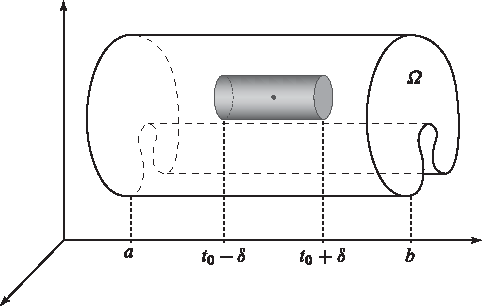
\includegraphics{./figuras-tikz/lipschitz.pdf}
  % \caption{}\label{fig:6.2}
\end{figure}
Definimos
\begin{equation*}
  X:=\left\{u\in \mathcal{C}^{0}([t_{0}-\delta ,t_{0}+\delta ],\mathbb{R}^{n}):\left\Vert u-x_{0}\right\Vert_{\infty }\leq \delta M\right\}
\end{equation*}
donde $x_{0}$ es la función constante con valor $x_{0}$ y
\begin{equation*}
  \left\Vert u\right\Vert_{\infty }=\max_{t\in [t_{0}-\delta
    ,t_{0}+\delta ]}\left\Vert u(t)\right\Vert
\end{equation*}
es la norma uniforme en $\mathcal{C}^{0}([t_{0}-\delta ,t_{0}+\delta
],\mathbb{R}^{n})$.\ Recuerda que $\mathcal{C}^{0}([t_{0}-\delta
,t_{0}+\delta ],\mathbb{R}^{n})$ es un espacio de Banach (ver Teorema
\ref{funcacotcompl}). Le damos a $X$ la métrica inducida por esta
norma.

\begin{lemma}

  \begin{enumerate}
  \item[(a)] $X$ es un espacio métrico completo.

  \item[(b)] Si $u\in X$, entonces $u(t)\in\bar{B}(x_{0},\delta_0)\subset\Omega $ para toda $t\in
    [t_{0}-\delta ,t_{0}+\delta ]$.
  \end{enumerate}
\end{lemma}

\begin{proof}
  \emph{(a):} \ Observa que $X$ es la bola cerrada con centro en la
  función constante $x_{0}$ y radio $\delta M$ en el espacio
  $\mathcal{C}^{0}([t_{0}-\delta ,t_{0}+\delta ],\mathbb{R}^{n})$ con
  la norma uniforme.  Por tanto, $X$ es un subconjunto cerrado de
  $\mathcal{C}^{0}([t_{0}-\delta ,t_{0}+\delta ],\mathbb{R}^{n})$. De
  la Proposición~\ref{complcerr}$\ $se sigue que $X$ es un espacio
  métrico completo.

  \emph{(b):} \ Si $u\in X$ entonces
  \begin{equation*}
    \left\Vert u(t)-x_{0}\right\Vert \leq \delta M<\delta_{0}\text{\qquad }\forall t\in [t_{0}-\delta ,t_{0}+\delta ].
  \end{equation*}
  En consecuencia, $u(t)\in \bar{B}(x_{0},\delta_{0})\subset \Omega $
  para toda $t\in [t_{0}-\delta ,t_{0}+\delta ]$.
\end{proof}

Para cada $u\in X$ definimos la función $\phi (u)\colon [t_{0}-\delta
,t_{0}+\delta ]\rightarrow \mathbb{R}^{n}$ como
\begin{equation*}
  \phi (u)(t):=\int_{t_{0}}^{t}\chi (s,u(s))ds+x_{0}.
\end{equation*}
Nota que el integrando está bien definido porque, de acuerdo con
el lema anterior, $u(s)\in \Omega $ para todo $s\in [t_{0}-\delta ,t_{0}+\delta ]$. Requerimos la siguiente desigualdad.

\begin{lemma}
  \label{lemcotint}Para cualquier función continua
  $f\colon [a,b]\rightarrow \mathbb{R}^{n}$\ se cumple que
  \begin{equation*}
    \biggl\Vert \int_{a}^{b}f(t)dt\biggr\Vert \leq \left\vert b-a\right\vert
    \left\Vert f\right\Vert_{\infty }.
  \end{equation*}
\end{lemma}

La demostración de esta desigualdad es sencilla y se propone como
ejercicio [Ejercicio~\ref{cotint}].

Probaremos ahora que $\phi $ es una función de $X$ en sí
mismo.

\begin{lemma}
  $\phi (u)\in X$ para todo $u\in X$.
\end{lemma}

\begin{proof}
  Por el teorema fundamental del cálculo, la $i$-ésima
  función componente de $\phi (u)$,
  \begin{equation*}
    \phi (u)_{i}(t):=\int_{t_{0}}^{t}\chi_{i}(s,u(s))ds+x_{0,i},
  \end{equation*}
  es continuamente diferenciable. En particular, $\phi (u)\in
  \mathcal{C}^{0}([t_{0}-\delta ,t_{0}+\delta
  ],\mathbb{R}^{n})$. Usando el Lema~\ref{lemcotint} obtenemos
  además que
  \begin{equation*}
    \left\Vert \phi (u)(t)-x_{0}\right\Vert =\left\Vert \int_{t_{0}}^{t}\chi
      (s,u(s))ds\right\Vert \leq \left\vert t-t_{0}\right\vert M\leq \delta M.
  \end{equation*}
  En consecuencia, $\phi(u)\in X$.
\end{proof}

\begin{multicols}{2}
\begin{bio}[H]
\centering

\includegraphics[width=.3\textwidth]{./fotos/calcasdos/Lindelof.pdf}\\[5pt]
{\small \bfseries Ernst Lindelöf}
\end{bio}
\begin{bio}[H]
\centering

\includegraphics[width=.3\textwidth]{./fotos/calcasdos/Charles_Emile_Picard.pdf}\\[5pt]
{\small \bfseries Émile Picard}
\end{bio}
\end{multicols}

El siguiente teorema es uno de los resultados fundamentales de la
teoría de ecuaciones diferenciales. Fue publicado por primera vez
en 1890 por Lindelöf\footnote{Ernst Leonard Lindelöf
  (1870-1946) nació en Helsinki, Finlandia. Se doctoró en la
  Universidad de Helsinki y fue profesor en esa
  universidad.}. Simultáneamente, Picard\footnote{Charles
  Émile Picard (1856-1941) nació en París. Estudió en
  la École Normale Supérieure bajo la supervisión de
  Gaston Darboux. Fue profesor en las universidades de París y
  Toulouse y de la École Normale.} desarrolló un método de
aproximación sucesiva de soluciones. El método de
iteración de Picard es justamente el método iterativo del
teorema de punto fijo de Banach para este caso particular.

\begin{theorem}[Picard-Lindelöf]
  \label{pl}\index{teorema!de Picard-Lindelöf}Sea $\chi
  \colon (a,b)\times \Omega \rightarrow \mathbb{R}^{n}$ una función
  continua y localmente Lipschitz continua en la segunda
  variable. Entonces, dados $t_{0}\in (a,b)$ y $x_{0}\in \Omega $,
  existe $\delta >0$ tal que el problema de Cauchy
  \emph{(\ref{cauchy})} tiene una única solución en el
  intervalo $[t_{0}-\delta ,t_{0}+\delta ]$.
\end{theorem}

\begin{proof}
  El lema anterior asegura que $\phi $ es una función de $X$ en
  sí mismo. Observa que $u\in X$ satisface la ecuación
  integral (\ref{intcau}) si y sólo si
  \begin{equation*}
    \phi (u)(t):=\int_{t_{0}}^{t}\chi (s,u(s))ds+x_{0}=u(t)\text{\qquad }\forall t\in [t_{0}-\delta ,t_{0}+\delta ],
  \end{equation*}
  es decir, si y sólo si $u$ es un punto fijo de $\phi\colon X\rightarrow X$.

  Probaremos que $\phi $ es una contracción. Sean $u,v\in X$.
  Usando el Lema~\ref{lemcotint} obtenemos que, para toda $t\in
  [t_{0}-\delta ,t_{0}+\delta ]$, se cumple que
  \begin{align*}
    \left\Vert \phi (u)(t)-\phi (v)(t)\right\Vert &=\left\Vert
      \int_{t_{0}}^{t}(\chi (s,u(s))-\chi (s,v(s)))ds\right\Vert \\
    &\leq \left\vert t-t_{0}\right\vert \max_{\left\vert s-t_{0}\right\vert
      \leq \delta }\left\Vert \chi (s,u(s))-\chi (s,v(s))\right\Vert \\
    &\leq \left\vert t-t_{0}\right\vert \max_{\left\vert s-t_{0}\right\vert
      \leq \delta }C\left\Vert u(s)-v(s)\right\Vert \\
    &\leq \delta C\left\Vert u-v\right\Vert_{\infty }.
  \end{align*}
  Por consiguiente,
  \begin{equation*}
    \left\Vert \phi (u)-\phi (v)\right\Vert_{\infty }\leq \delta C\left\Vert
      u-v\right\Vert_{\infty }
  \end{equation*}
  y, como hemos elegido $\delta $ tal que $\delta C<1$, se tiene que
  $\phi $ es una contracción.

  Como $X$ es completo, el Teorema~\ref{pf} asegura que $\phi $ tiene
  un único punto fijo. Es decir, que existe una única $u^{\ast
  }\in X$ que satisface la ecuación integral
  (\ref{intcau}).\emph{\ }Del Lema~\ref{int} se sigue que $u^{\ast }$
  es la única solución del problema de Cauchy (\ref{cauchy})
  en el intervalo $[t_{0}-\delta ,t_{0}+\delta ]$.
\end{proof}

\section{Ejercicios}

\begin{exercise}
  \label{metcont}Sea $X=X_{\disc}$ un espacio discreto \emph{(ver
    Ejemplo~\ref{disc})}. Prueba que $\phi \colon X\rightarrow X$ es una
  contracción si y sólo si $\phi $ es una función
  constante.
\end{exercise}

\begin{exercise}

  \begin{enumerate}
  \item[(a)] Prueba que la función $\phi
    \colon \mathbb{R}_{p}^{n}\rightarrow \mathbb{R}_{p}^{n}$ dada por $\phi
    (x)=\frac{1}{2}x$ es una contracción para todo $p\in [1,\infty )$.

  \item[(b)] ¿Es posible darle a $\mathbb{R}^{n}$
    alguna métrica tal que $\phi $ no sea contracción?

  \item[(c)] ¿Es posible darle a $\mathbb{R}^{n}$
    alguna norma tal que $\phi $ no sea contracción?
  \end{enumerate}
\end{exercise}

\begin{exercise}
  \label{pf1}

  \begin{enumerate}
  \item[(a)] Usa el teorema del valor intermedio para probar que toda
    función continua $f\colon [a,b]\rightarrow [a,b]$ tiene al
    menos un punto fijo.

  \item[(b)] Da un ejemplo de una función continua
    $f\colon [a,b]\rightarrow [a,b]$ con una infinidad de puntos
    fijos.
  \end{enumerate}
\end{exercise}

\begin{exercise}
  Sea $f\colon [a,b]\rightarrow \mathbb{R}$ una función continuamente
  diferenciable en $[a,b]$ y tal que $f(a)<0<f(b)$ y $f^{\prime
  }(x)>0$ para toda $x\in [a,b]$. Prueba que existe un
  único $x^{\ast }\in [a,b]$ tal que $f(x^{\ast })=0$ y que
  $x^{\ast }$ se puede encontrar por el método de aproximaciones
  sucesivas. \emph{(Sugerencia: Demuestra que existe }$\lambda
  >0$\emph{\ tal que }$x-\lambda f(x)\in [a,b]$\emph{\ para
    todo }$x\in [a,b]$\emph{\ y tal que }$\phi_{\lambda
  }(x):=x-\lambda f(x)$\emph{\ es una contracción en
  }$[a,b]$.\emph{)}
\end{exercise}

\begin{exercise}
  Prueba que, si $f\colon \mathbb{R}\rightarrow \mathbb{R}$ es continuamente
  diferenciable y $\left\vert f^{\prime }(x)\right\vert \leq M<1$ para
  todo $x\in \mathbb{R}$, entonces $f$ es una contracción.
\end{exercise}

\begin{exercise}
  Da un ejemplo de un espacio métrico completo y una función
  $\phi \colon X\rightarrow X$ que satisface
  \begin{equation}
    d(\phi (x),\phi (y))<d(x,y)\text{\qquad }\forall x,y\in X\text{ con }x\neq y,
    \label{contdebil}
  \end{equation}
  y que no tiene ningún punto fijo. Es decir, la condición
  \emph{(\ref{contdebil})} no es suficiente para garantizar la
  existencia de un punto fijo.
\end{exercise}

\begin{exercise}
  Prueba que, si $X$ es un espacio métrico compacto y $\phi
  \colon X\rightarrow X $ satisface
  \begin{equation*}
    d(\phi (x),\phi (y))<d(x,y)\text{\qquad }\forall x,y\in X\text{ \ con }x\neq
    y,
  \end{equation*}
  entonces $\phi $ tiene un único punto fijo.
\end{exercise}

\begin{exercise}
  Sean $X$ un espacio métrico completo y $\phi \colon X\rightarrow X$
  una función continua.

  \begin{enumerate}
  \item[(a)] Prueba que, si existe $\alpha \in (0,1)$ tal que
    \begin{equation*}
      d(\phi^{2}(x),\phi (x))\leq \alpha d(\phi (x),x)\text{\qquad }\forall x\in
      X,
    \end{equation*}
    entonces $\phi $ tiene un punto fijo.

  \item[(b)] Muestra, mediante un ejemplo, que dicho punto fijo no
    necesariamente es único.

  \item[(c)] Si $\phi $ no es continua, ¿es
    válida la afirmación (a)?
  \end{enumerate}
\end{exercise}

\begin{exercise}
  \label{ejsl}Sea $\ \phi \colon \mathbb{R}^{n}\rightarrow \mathbb{R}^{n}$
  la función dada por $\phi (x)=Ax-b$, donde $A=(a_{ij})$ es una
  matriz de $n\times n$ y $b\in \mathbb{R}^{n}$.

  \begin{enumerate}
  \item[(a)] Prueba que, si
    \begin{equation}
      \sum_{i=1}^{n}\sum_{j=1}^{n}a_{ij}^{2}<1,  \label{sl2}
    \end{equation}
    entonces $\phi \colon \mathbb{R}_{2}^{n}\rightarrow \mathbb{R}_{2}^{n}$
    es una contracción.

  \item[(b)] Prueba que, si
    \begin{equation}
      \max_{i=1,\dots,n}\sum_{j=1}^{n}\left\vert a_{ij}\right\vert <1,
      \label{slinf}
    \end{equation}
    entonces $\phi \colon \mathbb{R}_{\infty }^{n}\rightarrow
    \mathbb{R}_{\infty }^{n}$ es una contracción.

  \item[(c)] Da ejemplos de matrices $A$ que satisfagan cada una de
    las condiciones \emph{(\ref{sl1})}, \emph{(\ref{sl2})} y
    \emph{(\ref{slinf})} pero no las otras dos. Es decir, cada una de
    estas condiciones es suficiente para que la ecuación
    \begin{equation*}
      Ax-x=b,
    \end{equation*}
    tenga solución única, pero ninguna es necesaria.

  \item[(d)] En cada uno de los incisos (a) y (b) aplica la
    fórmula \emph{(\ref{error})} para estimar la solución en
    términos de $A$ y $b$ exclusivamente.

  \item[(e)] Prueba que cada una de las condiciones \emph{(\ref{sl2})}
    y \emph{(\ref{slinf})} implica que $\det (A-I)\neq 0$.

  \item[(f)] Da un ejemplo de una matriz $A$ tal que $\det (A-I)\neq
    0$ y que no cumple ninguna de las condiciones \emph{(\ref{sl1})},
    \emph{(\ref{sl2})} y \emph{(\ref{slinf}).}
  \end{enumerate}
\end{exercise}

\begin{exercise}
  Sea $A$ una matriz de $n\times n$. Recuerda que $\lambda \in
  \mathbb{R}$ es un valor propio de $A$ si existe $x\in
  \mathbb{R}^{n}$, $x\neq 0$, tal que $Ax=\lambda x$. Prueba que todo
  valor propio $\lambda $ de $A$ satisface
  \begin{equation*}
    \left\vert \lambda \right\vert \leq
    \max_{i=1,\dots,n}\sum_{j=1}^{n}\left\vert a_{ij}\right\vert .
  \end{equation*}
\end{exercise}

\begin{exercise}
  \label{ejopfred}Sea $\mathcal{K}\colon [a,b]\times [a,b]\rightarrow
  \mathbb{R}$ una función continua.

  \begin{enumerate}
  \item[(a)] Prueba que el operador de Fredholm
    $\mathfrak{F}\colon \mathcal{C}^{0}[a,b]\rightarrow
    \mathcal{C}^{0}[a,b]$ dado por
    \begin{equation*}
      (\mathfrak{F}f)(x):=\int_{a}^{b}\mathcal{K}(x,y)f(y)dy
    \end{equation*}
    es un operador lineal, es decir,
    \begin{equation*}
      \mathfrak{F}(\mu_{1}f_{1}+\mu_{2}f_{2})=\mu_{1}\mathfrak{F}(f_{1})+\mu
     _{2}\mathfrak{F}(f_{2})\text{\qquad }\forall f_{1},f_{2}\in \mathcal{C}^{0}[a,b],\text{ \ }\forall \mu_{1},\mu_{2}\in \mathbb{R}\text{.}
    \end{equation*}

  \item[(b)] $\mathfrak{F}\colon \mathcal{C}^{0}[a,b]\rightarrow
    \mathcal{C}^{0}[a,b] $ es Lipschitz continuo.
  \end{enumerate}
\end{exercise}

\begin{exercise}
  Sean $\mathcal{K}\colon [a,b]\times [a,b]\rightarrow \mathbb{R}$ \
  y $\ g\colon [a,b]\rightarrow \mathbb{R}$ funciones continuas, y sea
  $\lambda \in \mathbb{R}$ tal que $\left\vert \lambda \right\vert
  >\left\Vert \mathcal{K}\right\Vert_{\infty }(b-a)$. Prueba que la
  solución $f^{\ast }$ de la ecuación integral de Fredholm
  \emph{(\ref{fred})} satisface
  \begin{equation*}
    \left\Vert f^{\ast }-\sum_{m=1}^{k}\frac{1}{\lambda^{m}}\,\mathfrak{F}^{m-1}g\right\Vert_{\infty }\leq \frac{\alpha^{k}}{\left( 1-\alpha \right)
      \left\vert \lambda \right\vert }\left\Vert g\right\Vert_{\infty },
  \end{equation*}
  donde $\alpha :=\frac{1}{\left\vert \lambda \right\vert }\left\Vert
    \mathcal{K}\right\Vert_{\infty }(b-a)$ y $\mathfrak{F}$ es el
  operador de Fredholm.
\end{exercise}

\begin{exercise}
  Considera la ecuación no lineal de
  Fredholm\index{ecuación!no lineal de Fredholm}
  \begin{equation*}
    \lambda f(x)-\int_{a}^{b}\mathcal{K}(x,y,f(y))dy=g(x),
  \end{equation*}
  donde $\mathcal{K}\colon [a,b]\times [a,b]\times
  \mathbb{R}\rightarrow \mathbb{R}$ \ y $g\colon [a,b]\rightarrow
  \mathbb{R}$ son funciones continuas, y $\mathcal{K}$ es Lipschitz
  continua en la tercera variable, es decir, existe $M>0$ tal que
  \begin{equation*}
    \left\vert \mathcal{K}(x,y,z_{1})-\mathcal{K}(x,y,z_{2})\right\vert \leq
    M\left\vert z_{1}-z_{2}\right\vert 
    \text{\qquad }\forall x,y\in [a,b],\text{ \ }\forall z_{1},z_{2}\in 
    \mathbb{R}\text{.}
  \end{equation*}
  Prueba que esta ecuación tiene solución única si
  \begin{equation*}
    \left\vert \lambda \right\vert >M(b-a).
  \end{equation*}
\end{exercise}

\begin{exercise}
  Sea $\mathcal{K}\colon [a,b]\times [a,b]\rightarrow \mathbb{R}$ una
  función continua.

  \begin{enumerate}
  \item[(a)] Prueba que el operador de Volterra
    $\mathfrak{V}\colon \mathcal{C}^{0}[a,b]\rightarrow
    \mathcal{C}^{0}[a,b]$ dado por
    \begin{equation*}
      \left( \mathfrak{V}f\right) (x):=\int_{a}^{x}\mathcal{K}(x,y)f(y)dy
    \end{equation*}
    es un operador lineal, es decir,
    \begin{equation*}
      \mathfrak{V}(\mu_{1}f_{1}+\mu_{2}f_{2})=\mu_{1}\mathfrak{V}(f_{1})+\mu
     _{2}\mathfrak{V}(f_{2})\text{\qquad }\forall f_{1},f_{2}\in \mathcal{C}^{0}[a,b],\text{ \ }\forall \mu_{1},\mu_{2}\in \mathbb{R}\text{.}
    \end{equation*}

  \item[(b)] Prueba que $\mathfrak{V}\colon \mathcal{C}^{0}[a,b]\rightarrow
    \mathcal{C}^{0}[a,b]$ es Lipschitz continuo.

  \item[(c)] Prueba que, si $\lambda $ es un valor propio de
    $\mathfrak{V}$, entonces $\lambda =0$.
  \end{enumerate}
\end{exercise}

% \begin{exercise}
%   Sean $\mathcal{K}\colon [a,b]\times [a,b]\rightarrow \mathbb{R}$ \
%   y $\ g\colon [a,b]\rightarrow \mathbb{R}$ funciones continuas, y $\lambda
%   \neq 0$. Prueba que la solución $f^{\ast }$ de la ecuación
%   integral de Volterra (\ref{volterra}) satisface
%   \begin{equation*}
%     \left\Vert f^{\ast }-\sum_{m=1}^{k}\frac{1}{\lambda^{m}}\,\mathfrak{V}^{m-1}g\right\Vert_{\infty }\leq \frac{\alpha^{k}}{\left( 1-\alpha \right)
%       \left\vert \lambda \right\vert }\left\Vert g\right\Vert_{\infty },
%   \end{equation*}
%   donde $\alpha :=\frac{1}{\left\vert \lambda \right\vert }\left\Vert
%     \mathcal{K}\right\Vert_{\infty }(b-a)$ y $\mathfrak{V}$ es el
%   operador de Volterra.
% \end{exercise}

\begin{exercise}
  \label{cotint}Dada una función continua
  $f=(f_{1},\dots,f_{n})\colon [a,b]\rightarrow \mathbb{R}^{n}$,\ denotamos
  por
  \begin{equation*}
    \int_{a}^{b}f(t)dt:=\left(
      \int_{a}^{b}f_{1}(t)dt,\dots,\int_{a}^{b}f_{n}(t)dt\right) \in \mathbb{R}^{n}
  \end{equation*}
  al vector cuyas componentes son las integrales de las componentes de
  $f$. Prueba que
  \begin{equation*}
    \left\Vert \int_{a}^{b}f(t)dt\right\Vert \leq \left\vert b-a\right\vert
    \left\Vert f\right\Vert_{\infty },
  \end{equation*}
  donde $\left\Vert \cdot \right\Vert $ es la norma usual en
  $\mathbb{R}^{n}$ y $\left\Vert f\right\Vert_{\infty }=\sup_{t\in
    [a,b]}\left\Vert f(t)\right\Vert $ es la norma uniforme en
  $\mathcal{C}^{0}([a,b],\mathbb{R}^{n})$. \emph{(Sugerencia: Aplica
    primero la desigualdad de Hölder para probar que}
  \begin{equation*}
    \left\vert \int_{a}^{b}f_{i}\right\vert \leq \left( b-a\right)^{1/2}\left(
      \int_{a}^{b}\left\vert f_{i}\right\vert^{2}\right)^{1/2}
  \end{equation*}
  \emph{para }$i=1,\dots,n\emph{).}$
\end{exercise}

\begin{exercise}
  Prueba que, si $f\colon \mathbb{R}\rightarrow \mathbb{R}$ es continuamente
  diferenciable, entonces es localmente Lipschitz continua, es decir,
  para cada $t\in \mathbb{R}$, existe $\delta_{t}>0$ tal que la
  restricción de $f$ al intervalo $[t-\delta_{t},t+\delta_{t}]$
  es Lipschitz continua.
\end{exercise}

\begin{exercise}
  \label{ejnounica}Sea $\chi \colon \mathbb{R\times R}\rightarrow
  \mathbb{R}$ tal que $\chi (t,x)=3x^{2/3}$.

  \begin{enumerate}
  \item[(a)] Prueba que $\chi $ no es localmente Lipschitz continua en
    la segunda variable.

  \item[(b)] Prueba que, para cualesquiera $\alpha <0<\beta $, la
    función
    \begin{equation*}
      u_{\alpha ,\beta }(t):=
        \begin{cases}
          (t-\alpha )^{3} & \text{si $t\leq \alpha$,} \\ 
          0 & \text{si $\alpha \leq t\leq \beta$,} \\ 
          (t-\beta )^{3} & \text{si $t\geq \beta$,}
        \end{cases}
    \end{equation*}
    es diferenciable en $\mathbb{R}$\ y es solución del problema
    de Cauchy
    \begin{equation*}
        \begin{cases}
          u^{\prime }=3u^{2/3}, \\ 
          u(0)=0.
        \end{cases}
    \end{equation*}
    En consecuencia, si $\chi $ no es localmente Lipschitz continua en
    la segunda variable, el problema de Cauchy puede tener una
    infinidad de soluciones.
  \end{enumerate}
\end{exercise}

\begin{exercise}
  Sea $\chi \colon \mathbb{R\times R}\rightarrow \mathbb{R}$ tal que $\chi
  (t,x)=-x^{2}$.

  \begin{enumerate}
  \item[(a)] Prueba que $\chi $ es localmente Lipschitz continua en la
    segunda variable.

  \item[(b)] Para $\alpha \neq 0$ considera el problema de Cauchy
    \begin{equation}
      \begin{cases}
        u^{\prime }=-u^{2}, \\ 
        u(0)=-\frac{1}{\alpha }.
      \end{cases}
      \label{pej}
    \end{equation}
    Prueba que
    \begin{equation*}
      u(t)=\frac{1}{t-\alpha }
    \end{equation*}
    es solución de \emph{(\ref{pej})} en algún intervalo que
    contiene a $0$.

  \item[(c)] ¿Cuál es el intervalo máximo
    para el que existe una solución de \emph{(\ref{pej})}?
  \end{enumerate}
\end{exercise}

\chapter{Compacidad en espacios de funciones}

\label{caparzelaascoli}En el Capítulo~\ref{capcomp}\ dimos una
caracterización sencilla de los subconjuntos compactos de
$\mathbb{R}^{n} $. Probamos que son precisamente aquellos que son
cerrados y acotados.

El objetivo de este capítulo es dar una caracterización
sencilla de los subconjuntos compactos del espacio de funciones
continuas $\mathcal{C}^{0}(K,X)$ en un espacio métrico compacto
$K$. Dicha caracterización, debida a Giulio Ascoli y Cesare
Arzelà, se basa fundamentalmente en la noción de
\emph{equicontinuidad}.

El teorema de Arzelà-Ascoli es un resultado fundamental en
análisis y tiene muchas aplicaciones importantes. Una de ellas es
el teorema de Peano que afirma la existencia de soluciones al problema
de Cauchy para campos vectoriales continuos. Lo demostraremos en este
capítulo.

Además aplicaremos el teorema de Arzelà-Ascoli para obtener
condiciones que aseguren la existencia de trayectorias de longitud
mínima en espacios métricos, dando así respuesta a la
pregunta que planteamos en el Capítulo~\ref{capmotivacion}.

\section{Conjuntos totalmente acotados}

La demostración del teorema de Heine-Borel se basó en el hecho
de que podemos cubrir a un cubo en $\mathbb{R}^{n}$ (y, en
consecuencia, a cualquier subconjunto acotado) con un número
finito de bolas de radio $\varepsilon $, para cualquier $\varepsilon
>0$. Esto no es cierto en un espacio métrico arbitrario, como lo
muestra el siguiente ejemplo.

\begin{example}
  \label{nota}La bola cerrada $\ \bar{B}_{\ell
   _{2}}(0,1):=\left\{(x_{n})\in \ell_{2}:\sum_{n=1}^{\infty
  }x_{n}^{2}\leq 1\right\}$\textbf{\ } no puede ser cubierta por un
  número finito de bolas abiertas de radio $\varepsilon $ en $\ell
 _{2}$, para ningún $\varepsilon \in (0,\sqrt{2}/2)$.
\end{example}

\begin{proof}
  Para cada $k\in \mathbb{N}$ denotemos por $\overline{e}_{k}\in \ell
 _{2}$ a la sucesión cuyo $k$-ésimo término es $1$ y
  todos los demás términos son $0$. Claramente
  $\overline{e}_{k}\in \bar{B}_{\ell_{2}}(0,1)$. Observa que
  \begin{equation*}
    \left\Vert \overline{e}_{j}-\overline{e}_{k}\right\Vert_{2}=\sqrt{2}\text{\qquad }\forall j\neq k.
  \end{equation*}
  Sea $\varepsilon \in (0,\sqrt{2}/2)$. Si $\bar{B}_{\ell_{2}}(0,1)$
  pudiese ser cubierta por un número finito de bolas de radio
  $\varepsilon $ en $\ell_{2}$, entonces al menos una de ellas
  tendría que contener a un par de sucesiones
  $\overline{e}_{j},\overline{e}_{k}$ con $j\neq k$, lo cual es
  imposible.
\end{proof}

Sea $X=(X,d_{X})$ un espacio métrico. Estudiaremos a los
subconjuntos de $X$ que tienen la siguiente propiedad.

\begin{definition}
  Un subconjunto $A$ de $X$ es \textbf{totalmente acotado
  }\index{conjunto!totalmente acotado}\index{totalmente acotado}si
  para cada $\varepsilon >0$ existe un número finito de puntos
  $a_{1},\dots,a_{m}\in A$ tales que
  \begin{equation*}
    A\subset B_{X}(a_{1},\varepsilon )\cup \cdots \cup B_{X}(a_{m},\varepsilon ),
  \end{equation*}
  donde $B_{X}(a,\varepsilon )$ denota a la bola abierta con centro en
  $a$ y radio $\varepsilon $ en $X$.
\end{definition}

Veamos algunas propiedades sencillas de los conjuntos totalmente
acotados.

\begin{proposition}
  \label{propta}Sea $A$ un subconjunto de $X$.

  \begin{enumerate}
  \item[(a)] Si $A$ es compacto, entonces $A$ es totalmente acotado.

  \item[(b)] Si $A$ es totalmente acotado, entonces $A$ es acotado en
    $X$.

  \item[(c)] Si $D\subset A$ y $A$ es totalmente acotado, entonces $D$
    es totalmente acotado.

  \item[(d)] Si $A$ es totalmente acotado, entonces su cerradura
    $\overline{A}$ en $X$ es totalmente acotada.
  \end{enumerate}
\end{proposition}

\begin{proof}
  \emph{(a): } Si $A\subset X$ es compacto entonces, para toda
  $\varepsilon >0$, la cubierta abierta $\left\{B_{X}(x,\varepsilon ):x\in
  A\right\}$ de $A$ contiene una subcubierta finita. Es decir, existen
  $x_{1},\dots,x_{m}\in A$ tales que
  \begin{equation*}
    A\subset B_{X}(x_{1},\varepsilon )\cup \cdots \cup B_{X}(x_{m},\varepsilon ).
  \end{equation*}

  \emph{(b): } Si $A\subset X$ es totalmente acotado entonces existen
  $a_{1},\dots,a_{m}\in A$ tales que
  \begin{equation*}
    A\subset B_{X}(a_{1},1)\cup \cdots \cup B_{X}(a_{m},1).
  \end{equation*}
  En consecuencia, $A\subset B_{X}(a_{1},r+1)$ donde $r:=\max
  \left\{d_{X}(a_{1},a_{j}):j=2,\dots,m\right\}$, es decir, $A$ es acotado.

  \emph{(c): } Sean $A$ un subconjunto totalmente acotado de $X$,
  $D\subset A$ y $\varepsilon >0$. Entonces existen
  $a_{1},\dots,a_{m}\in A$ tales que
  \begin{equation*}
    A\subset B_{X}(a_{1},\tfrac{\varepsilon }{2})\cup \cdots \cup B_{X}(a_{m},\tfrac{\varepsilon }{2}).
  \end{equation*}
  Sea $J:=\left\{j\in \left\{1,\dots,m\right\}:B_{X}(a_{j},\frac{\varepsilon }{2})\cap
  D\neq \emptyset \right\}$. Para cada $j\in J$ elegimos un punto $b_{j}\in
  B_{X}(a_{j},\frac{\varepsilon }{2})\cap D$. Entonces se cumple que
  \begin{equation*}
    D\subset \bigcup_{j\in J}B_{X}(b_{j},\varepsilon ).
  \end{equation*}
  Esto prueba que $D$ es totalmente acotado.

  \emph{(d): } Sean $A$ un subconjunto totalmente acotado de $X$,
  $\varepsilon >0$, y $a_{1},\dots,a_{m}\in A$ tales que
  \begin{equation*}
    A\subset B_{X}(a_{1},\tfrac{\varepsilon }{2})\cup \cdots \cup B_{X}(a_{m},\tfrac{\varepsilon }{2}).
  \end{equation*}
  Como \ $\bar{B}_{X}(a_{1},\frac{\varepsilon }{2})\cup \cdots \cup
  \bar{B}_{X}(a_{m},\frac{\varepsilon }{2})$ \ es cerrado, se tiene
  que
  \begin{equation*}
    \overline{A}\subset \bar{B}_{X}(a_{1},\tfrac{\varepsilon }{2})\cup \cdots
    \cup \bar{B}_{X}(a_{m},\tfrac{\varepsilon }{2}).
  \end{equation*}
  En consecuencia,
  \begin{equation*}
    \overline{A}\subset B_{X}(a_{1},\varepsilon )\cup \cdots \cup
    B_{X}(a_{m},\varepsilon ).
  \end{equation*}
  Esto prueba que $\overline{A}$ es totalmente acotado.
\end{proof}

El siguiente resultado da caracterizaciones muy útiles de los
espacios métricos compactos.

\begin{theorem}
  \label{caractcomp}Las siguientes tres afirmaciones son equivalentes:

  \begin{enumerate}
  \item[(a)] $X$ es compacto.

  \item[(b)] Toda sucesión en $X$ contiene una subsucesión que
    converge en $X$.

  \item[(c)] $X$ es completo y totalmente acotado.
  \end{enumerate}
\end{theorem}

\begin{proof}
  \emph{(a)\thinspace }$\Rightarrow $\emph{\thinspace (b)}: \ Esta
  es la afirmación de la Proposición~\ref{compbw}.

  \emph{(b)\thinspace }$\Rightarrow $\emph{\thinspace (c)}: \ Sea
  $(x_{k})$ una sucesión de Cauchy en $X$. Si $X$ satisface
  \emph{(b)} entonces $(x_{k})$ contiene una subsucesión que
  converge a un punto $x\in X$. En consecuencia, $(x_{k})$ converge a
  $x$ en $X$ (ver Ejercicio~\ref{subconvcau}). Esto prueba que $X$
  es completo.

  Supongamos ahora que $X$ no es totalmente acotado. Entonces existe
  $\varepsilon_{0}>0$ tal que $X$ no puede ser cubierto por un
  número finito de bolas abiertas de radio $\varepsilon_{0}$. Por
  consiguiente, podemos escoger, inductivamente, una sucesión de
  puntos $x_{k}\in X$ tales que
  \begin{equation*}
    x_{k}\notin B_{X}(x_{1},\varepsilon_{0})\cup \cdots \cup
    B_{X}(x_{k-1},\varepsilon_{0}).
  \end{equation*}
  Por tanto, $d_{X}(x_{j},x_{k})\geq \varepsilon_{0}$ para toda
  $j\neq k$ y, en consecuencia, ninguna subsucesión de $(x_{k})$
  es de Cauchy. Esto implica que $(x_{k})$ no contiene ninguna
  subsucesión convergente. Es decir, si $X$ no es totalmente
  acotado, entonces \emph{(b)} no se cumple.

  \emph{(c)\thinspace }$\Rightarrow $\emph{\thinspace (a)}: \
  Argumentando por contradicción, supongamos que $X$ es completo y
  totalmente acotado pero no es compacto. Entonces $X$ tiene una
  cubierta abierta $\mathcal{U}=\left\{U_{i}:i\in \mathcal{I}\right\}$
  que no contiene ninguna subcubierta finita.  Como $X$ es totalmente
  acotado, está contenido en la unión de un número finito de bolas
  abiertas de radio $1$. Por tanto, existe un punto $x_{0}\in X$ tal
  que $B_{X}(x_{0},1)$, no puede ser cubierta por un número finito de
  elementos de $\mathcal{U}$. Como $B_{X}(x_{0},1)$ es totalmente
  acotado (ver Proposición~\ref{propta}), está contenido en la unión
  de un número finito de bolas abiertas de radio $\frac{1}{2}$ cuyos
  centros están en $B_{X}(x_{0},1)$. Por consiguiente, existe
  $x_{1}\in B_{X}(x_{0},1)$ tal que $B_{X}(x_{1},\frac{1}{2})$, no
  puede ser cubierta por un número finito de elementos de
  $\mathcal{U}$. De este modo construímos, inductivamente, una
  sucesión $(x_{k})$ tal que
  $x_{k}\in B_{X}(x_{k-1},\frac{1}{2^{k-1}}) $ \ y \
  $B_{X}(x_{k},\frac{1}{2^{k}})$ \ no puede ser cubierta por un número
  finito de elementos de $\mathcal{U}$. Para toda $j\geq k$, se tiene
  entonces que
  \begin{equation}
    d_{X}(x_{k},x_{j})\leq d_{X}(x_{k},x_{k+1})+\cdots +d_{X}(x_{j-1},x_{j})<\tfrac{1}{2^{k}}+\cdots +\tfrac{1}{2^{j-1}}<\tfrac{1}{2^{k-1}},  \label{desta}
  \end{equation}
  es decir, la sucesión $(x_{k})$ es Cauchy. Como $X$ es completo,
  esta sucesión converge a un punto $x^{\ast }\ $en $X$. Haciendo
  tender $j\rightarrow \infty $ en la desigualdad (\ref{desta})
  obtenemos que
  \begin{equation*}
    d_{X}(x_{k},x^{\ast })\leq \tfrac{1}{2^{k-1}}\text{\qquad }\forall k\in 
    \mathbb{N}.
  \end{equation*}
  Por otra parte, como $x^{\ast }\in X$, existe $U^{\ast }\in
  \mathcal{U}$ tal que $x^{\ast }\in U^{\ast }$. Como $U^{\ast }$ es
  abierto, existe $\varepsilon >0$ tal que $B_{X}(x^{\ast
  },\varepsilon )\subset U^{\ast }$. Sea $k$ tal que
  $\frac{1}{2^{k-1}}<\frac{\varepsilon }{2}$. Entonces, para todo
  $x\in B_{X}(x_{k},\frac{1}{2^{k}})$, se tiene que
  \begin{equation*}
    d_{X}(x,x^{\ast })\leq d_{X}(x,x_{k})+d_{X}(x^{\ast },x_{k})<\tfrac{1}{2^{k}}+\tfrac{1}{2^{k-1}}<\varepsilon ,
  \end{equation*}
  es decir,
  \begin{equation*}
    B_{X}(x_{k},\tfrac{1}{2^{k}})\subset B_{X}(x^{\ast },\varepsilon )\subset
    U^{\ast }.
  \end{equation*}
  Esto es una contradicción, ya que habíamos supuesto que
  $B_{X}(x_{k},\frac{1}{2^{k}})$ no puede ser cubierta por un
  número finito de elementos de $\mathcal{U}$.
\end{proof}

Observa la similitud de la demostración de la afirmación
\emph{(c)\thinspace }$\Rightarrow $\emph{\thinspace (a)} con la de la
Proposición~\ref{cubo}, que constituye la parte medular de la
demostración del teorema de Heine-Borel. La caracterización
\emph{(c)} es muy útil, como veremos en las siguientes secciones.

\begin{definition}
  Un subconjunto $A$ de $X$ es \textbf{relativamente compacto}
  \index{conjunto!relativamente compacto}\index{relativamente
    compacto}en $X$ si su cerradura $\overline{A}$ en $X$ es compacta.
\end{definition}

Los subconjuntos relativamente compactos de $\mathbb{R}^{n}$ son
precisamente los conjuntos acotados.

En un espacio métrico completo se cumple lo siguiente.

\begin{corollary}
  \label{relcomp=ta}Un subconjunto $A$ de un espacio métrico
  completo $X$ es relativamente compacto en $X$ si y sólo si es
  totalmente acotado.
\end{corollary}

\begin{proof}
  $\Rightarrow )$: \ Sea $A$ relativamente compacto en $X$. La
  Proposición~\ref{propta} implica entonces que $\overline{A}$ es
  totalmente acotado y, en consecuencia, que $A$ también lo es.

  $\Leftarrow )$: \ Inversamente, supongamos que $A$ es totalmente
  acotado. La Proposición~\ref{propta} afirma que $\overline{A}$ es
  totalmente acotado. Por otra parte, como $X$ es completo y
  $\overline{A}$ es cerrado en $X$, se tiene que $\overline{A}$ es
  completo (ver Proposición~\ref{complcerr}). El
  Teorema~\ref{caractcomp} asegura entonces que $\overline{A}$\ es
  compacto.
\end{proof}

\section{El teorema de Arzelà-Ascoli}

Sean $K=(K,d_{K})$ un espacio métrico compacto y $X=(X,d_{X})$ un
espacio métrico. Consideremos el espacio de funciones continuas
{\abovedisplayskip=7pt
\belowdisplayskip=7pt
\begin{equation*}
  \mathcal{C}^{0}(K,X):=\left\{f\colon K\rightarrow X:f\text{ es continua}\right\}
\end{equation*}
con la métrica uniforme
\begin{equation*}
  d_{\infty }(f,g)=\max_{z\in K}d_{X}(f(z),g(z)),
\end{equation*}
ver (\ref{dinfmax}). Usaremos el Corolario~\ref{relcomp=ta} para
obtener una caracterización sencilla de los subconjuntos
relativamente compactos de $\mathcal{C}^{0}(K,X)$. La siguiente
noción, introducida por Ascoli en 1884, jugará un papel
fundamental.

\begin{definition}
  Un subconjunto $\mathcal{H}$ de $\mathcal{C}^{0}(K,X)$ es
  \textbf{equicontinuo}
  \index{conjunto!equicontinuo}\index{equicontinuo}en el punto
  $z_{0}\in K$ si, para cada $\varepsilon >0$, existe $\delta >0$ (que
  depende de $\varepsilon $ y de $z_{0}$) tal que, para toda $f\in
  \mathcal{H}$,
  \begin{equation*}
    d_{X}\left( f(z),f(z_{0})\right) <\varepsilon 
    \text{\qquad si \ }d_{K}\left( z,z_{0}\right) <\delta .
  \end{equation*}
  $\mathcal{H}$ es \textbf{equicontinuo }si lo es en todo punto de
  $K$.
\end{definition}
}

El aspecto crucial de esta definición es que la misma $\delta >0$
nos sirve para todas las funciones que pertenecen a $\mathcal{H}$. Un
ejemplo en el que esto no se cumple es el siguiente.

\begin{example}
  El conjunto $\mathcal{H}=\left\{f_{k}\in
  \mathcal{C}^{0}([-1,1],\mathbb{R}):k\in \mathbb{N}\right\}$, donde
  \begin{equation*}
    f_{k}(t)=
      \begin{cases}
        -1 & \text{si $t\in \left[ -1,-\frac{1}{k}\right]$,} \\[3pt] 
        kt & \text{si $t\in \left[ -\frac{1}{k},\frac{1}{k}\right]$,} \\[3pt] 
        1 & \text{si $t\in \left[ \frac{1}{k},1\right]$,}
      \end{cases}
  \end{equation*}
  no es equicontinuo en $0$.
\begin{figure}[htb]
  \centering
  \begin{tikzpicture}[scale=1.7]
  \draw (-1,0)--(1,0);
  \draw (0,-1)--(0,1);
  \draw[very thick] (-1,-1)--(-.333,-1)--(.333,1)--(1,1);
  \foreach \x in {-0.5, 0.5, -1, 1}{
               \draw[thin] (-.025,\x)--(0.025,\x);
};
  \foreach \x in {-1, 1}{
               \draw[thin] (\x,-0.025)--(\x,0.025);
};

\draw[dashed] (-.333,0) -- (-.333,-1);
\draw[dashed] (.333,0) -- (.333,1);
\draw (0,-1.2) node[below] {$y=f_k(x)$};

\draw (.333,-.025) node[below] {$\frac{1}{k}$};
\draw (1,-.025) node[below] {$1$};
\draw (-.333,.025) node[above] {$-\frac{1}{k}$};
\draw (-1,-.025) node[below] {$-1$};
%\draw (-.025,.5) node[left] {$\frac{1}{2}$};
\draw (-.025,1) node[left] {$1$};
%\draw (.025,-.5) node[right] {$-\frac{1}{2}$};
\draw (.025,-1) node[right] {$-1$};
\end{tikzpicture}

  % \caption{}\label{fig:7.1}
\end{figure}
\end{example}

La demostración es sencilla [Ejercicio~\ref{noequi}].

A continuación enunciamos el teorema de Giulio
Ascoli\footnote{Giulio Ascoli (1843-1896) nació en Trieste,
  Italia. Estudió en la Scuola Normale di Pisa y fue profesor en
  el Politecnico di Milano.} y Cesare Arzelà\footnote{Cesare
  Arzelà (1847-1912) nació en Santo Stefano di Magra, Italia.
  Estudió en la Scuola Normale Superiore de Pisa, donde fue alumno
  de Enrico Betti y Ulisse Dini, y fue profesor en la Universidad de
  Bologna.}.

\begin{multicols}{2}
\begin{bio}[H]
\centering
%
\includegraphics[width=.3\textwidth]{./fotos/calcasdos/Frechet.png}\\[5pt]

\includegraphics[height=.31\textwidth]{./fotos/calcasdos/Giulio_ascoli.pdf}\\[5pt]
{\small \bfseries Giulio Ascoli}
\end{bio}
\begin{bio}[H]
\centering
%
\includegraphics[width=.3\textwidth]{./fotos/calcasdos/Frechet.png}\\[5pt]

\includegraphics[height=.31\textwidth]{./fotos/calcasdos/Arzela.pdf}\\[5pt]
{\small \bfseries Cesare Arzelà}
\end{bio}
\end{multicols}

Denotaremos por
\begin{equation*}
  B_{\infty }(f_{0},r):=\left\{f\in \mathcal{C}^{0}(K,X):d_{\infty }(f,f_{0})<r\right\}
\end{equation*}
a la bola abierta en $\mathcal{C}^{0}(K,X)$ con centro en $f_{0}$ y
radio $r. $

\begin{theorem}[Arzelà-Ascoli]
  \label{aa}\index{teorema!de Arzelà-Ascoli}Sean $K$ un espacio
  métrico compacto y $X$ un espacio métrico completo. Un
  subconjunto $\mathcal{H}$ de $\mathcal{C}^{0}(K,X)$ es relativamente
  compacto en $\mathcal{C}^{0}(K,X)$ si y sólo si $\mathcal{H}$ es
  equicontinuo y los conjuntos
  \begin{equation*}
    \mathcal{H}(z):=\left\{f(z):f\in \mathcal{H}\right\}
  \end{equation*}
  son relativamente compactos en $X$ para cada $z\in K$.
\end{theorem}

\begin{proof}
  $\Rightarrow )$: \ Supongamos que $\mathcal{H}$ es relativamente
  compacto en $\mathcal{C}^{0}(K,X)$. Entonces $\mathcal{H}$ es
  totalmente acotado. En consecuencia, dada $\varepsilon >0$, existen
  $g_{1},\dots,g_{m}\in \mathcal{H}$ tales que
  \begin{equation*}
    \mathcal{H}\subset B_{\infty }(g_{1},\tfrac{\varepsilon }{3})\cup 
    \cdots \cup B_{\infty }(g_{m},\tfrac{\varepsilon }{3}).
  \end{equation*}
  Por tanto, $g_{i}(z)\in \mathcal{H}(z)$ para $i=1,\dots,m$, y
  \begin{equation*}
    \mathcal{H}(z)\subset B_{X}(g_{1}(z),\tfrac{\varepsilon }{3})\cup \cdots \cup
    B_{X}(g_{m}(z),\tfrac{\varepsilon }{3})\text{\qquad }\forall z\in K.
  \end{equation*}
  Esto prueba que $\mathcal{H}(z)$ es totalmente acotado y, como $X$
  es completo, el Corolario~\ref{relcomp=ta}\ asegura que
  $\mathcal{H}(z)$ es relativamente compacto en $X$ para todo $z\in
  K$.

  Por otra parte, como $K$ es compacto, cada $g_{i}$ es uniformemente
  continua. En consecuencia, existe $\delta_{i}>0$ tal que, para
  cualesquiera $y,z\in K$,
  \begin{equation}
    d_{X}\left( g_{i}(y),g_{i}(z)\right) <\frac{\varepsilon }{3}\text{\qquad si }d_{K}(y,z)<\delta_{i}.  \label{gunifcon}
  \end{equation}
  Definimos $\delta :=\min \left\{\delta_{1},\dots,\delta_{m}\right\}$. Dada
  $f\in \mathcal{H}$ existe $i\in \left\{1,\dots,m\right\}$ tal que $d_{\infty
  }(f,g_{i})<\frac{\varepsilon }{3}$. Usando (\ref{gunifcon})
  obtenemos que
  \begin{align*}
    d_{X}(f(y),f(z)) &\leq
    d_{X}(f(y),g_{i}(y))+d_{X}(g_{i}(y),g_{i}(z))+d_{X}\left(
      g_{i}(z),f(z)\right) \\
    &<\varepsilon \text{\qquad si \ }d_{K}(y,z)<\delta .
  \end{align*}
  Esto prueba que $\mathcal{H}$\ es equicontinuo.

  $\Leftarrow )$: \ Supongamos ahora que $\mathcal{H}$ es equicontinuo
  y que $\mathcal{H}(z)$\ es relativamente compacto en $X$ para todo
  $z\in K$. Queremos probar que $\mathcal{H}$ es relativamente
  compacto en $\mathcal{C}^{0}(K,X)$. Como $X$ es completo,
  $\mathcal{C}^{0}(K,X)$ también lo es (ver
  Teorema~\ref{funcacotcompl}). Por el Corolario~\ref{relcomp=ta}\
  basta entonces probar que $\mathcal{H}$ es totalmente acotado.

{\abovedisplayskip=9.5pt plus 1pt minus 1pt
\belowdisplayskip=9.5pt plus 1pt minus 1pt
  Sea $\varepsilon >0$. Para cada $z\in K$ tomemos $\delta_{z}>0$ tal
  que, para toda $f\in \mathcal{H}$,
  \begin{equation}
    d_{X}\left( f(y),f(z)\right) <\frac{\varepsilon }{4}\text{ \quad si }d_{K}\left( y,z\right) <\delta_{z}.  \label{Hequi}
  \end{equation}
  Como $K$ es compacto, existen $z_{1},\dots,z_{m}\in K$ tales que
  \begin{equation}
    K\subset B_{K}(z_{1},\delta_{z_{1}})\cup \cdots \cup B_{K}(z_{m},\delta
   _{z_{m}})  \label{Xcomp}
  \end{equation}
  y, como cada $\mathcal{H}(z_{i})$\ es totalmente acotado, existen
  $x_{1},\dots,x_{k}\in X$ tales que
  \begin{equation}
    \mathcal{H}(z_{1})\cup \cdots \cup \mathcal{H}(z_{m})\subset B_{X}(x_{1},\tfrac{\varepsilon }{4})\cup \cdots \cup B_{X}(x_{k},\tfrac{\varepsilon }{4}).
    \label{Hta}
  \end{equation}
  Denotemos por $S$ al conjunto (finito) de todas las funciones
  $\sigma \colon \left\{1,\dots,m\right\}\rightarrow \left\{1,\dots,k\right\}$. Para cada $\sigma \in
  S$ definimos
  \begin{equation*}
    \mathcal{H}_{\sigma }:=\left\{f\in \mathcal{H}:f(z_{i})\in B_{X}(x_{\sigma (i)},\tfrac{\varepsilon }{4})\text{ \ }\forall i=1,\dots,m\right\}.
  \end{equation*}
  Se sigue de (\ref{Hta}) que, para cada $f\in \mathcal{H}$ y cada
  $i\in \left\{1,\dots,m\right\}$, existe $\sigma (i)\in \left\{1,\dots,k\right\}$ tal que
  $f(z_{i})\in B_{X}(x_{\sigma (i)},\frac{\varepsilon }{4})$. En
  consecuencia,
  \begin{equation}
    \mathcal{H}\subset \bigcup_{\sigma \in S}\mathcal{H}_{\sigma }.  \label{Hta1}
  \end{equation}
  Probaremos ahora que cada $\mathcal{H}_{\sigma }$ está contenida
  en una bola de radio $\varepsilon $ con centro en $\mathcal{H}$.
  Sean $f,g\in \mathcal{H}_{\sigma }$ y sea $z\in K$. Se sigue de
  (\ref{Xcomp}) que existe $i\in \left\{1,\dots,m\right\}$ tal que
  $d_{K}(z,z_{i})<\delta_{z_{i}}$ y, en consecuencia, (\ref{Hequi})
  implica que $d_{X}\left( h(z),h(z_{i})\right) <\frac{\varepsilon
  }{4}$ para toda $h\in \mathcal{H}$. Por tanto,
  \begin{align*}
    d_{X}(f(z),g(z)) &\leq d_{X}\left( f(z),f(z_{i})\right)
    +d_{X}(f(z_{i}),x_{\sigma (i)}) \\
    &\qquad{}+d_{X}(g(z_{i}),x_{\sigma (i)})+d_{X}\left( g(z),g(z_{i})\right)
    <\varepsilon .
  \end{align*}
  Tomando el máximo sobre toda $z\in K$ concluimos que $d_{\infty
  }(f,g)<\varepsilon $ para todas $f,g\in \mathcal{H}_{\sigma }$. En
  consecuencia, para cualquier elección de $g_{\sigma }\in
  \mathcal{H}_{\sigma }$, se cumple que
  \begin{equation}
    \mathcal{H}_{\sigma }\subset B_{\infty }(g_{\sigma },\varepsilon ).
    \label{Hta2}
  \end{equation}
  De (\ref{Hta1}) y (\ref{Hta2}) se sigue que
  \begin{equation*}
    \mathcal{H}\subset \bigcup_{\sigma \in S}B_{\infty }(g_{\sigma },\varepsilon
    ).
  \end{equation*}}
  Por tanto, $\mathcal{H}$ es totalmente acotado.
\end{proof}

Recordemos que $\mathcal{H}$ es un subconjunto acotado de
$\mathcal{C}^{0}(K,\mathbb{R}^{n})$ si existen $f_{0}\in \mathcal{H}$
y $C>0$ tales que
\begin{equation*}
  \left\Vert f-f_{0}\right\Vert_{\infty }=\max_{z\in K}\left\Vert
    f(z)-f_{0}(z)\right\Vert \leq C\text{\qquad }\forall f\in \mathcal{H}
\end{equation*}
(ver Definición~\ref{defconjacotado}). El teorema de
Arzelà-Ascoli permite caracterizar a los subconjuntos
relativamente compactos de $\mathcal{C}^{0}(K,\mathbb{R}^{n})$ como
sigue.

\begin{corollary}
  \label{coraa}Sea $K$ un espacio métrico compacto. Un subconjunto
  $\mathcal{H}$ de $\mathcal{C}^{0}(K,\mathbb{R}^{n})$ es
  relativamente compacto en $\mathcal{C}^{0}(K,\mathbb{R}^{n})$ si y
  sólo si $\mathcal{H} $ es equicontinuo y acotado en
  $\mathcal{C}^{0}(K,\mathbb{R}^{n})$.
\end{corollary}

\begin{proof}
  $\Rightarrow )$: \ Sea $\mathcal{H}$ un subconjunto relativamente
  compacto en $\mathcal{C}^{0}(K,\mathbb{R}^{n})$. Por el
  Teorema~\ref{aa}, $\mathcal{H} $ es equicontinuo y, por la
  Proposición~\ref{comphb},\ la cerradura de $\mathcal{H}$ es acotada
  en $\mathcal{C}^{0}(K,\mathbb{R}^{n})$. En consecuencia,
  $\mathcal{H}$ es acotado en $\mathcal{C}^{0}(K,\mathbb{R}^{n}). $

  $\Leftarrow )$: \ Inversamente, supongamos que $\mathcal{H}$ es
  equicontinuo y acotado en $\mathcal{C}^{0}(K,\mathbb{R}^{n})$.
  Entonces existen $f_{0}\in \mathcal{H}$ y $C>0$ tales que
  \begin{equation*}
    \left\Vert f-f_{0}\right\Vert_{\infty }=\max_{z\in K}\left\Vert
      f(z)-f_{0}(z)\right\Vert \leq C\text{\qquad }\forall f\in \mathcal{H}.
  \end{equation*}
  En consecuencia, $\mathcal{H}(z)$ está acotado en
  $\mathbb{R}^{n}$ para todo $z\in K$ y, por el teorema de Heine-Borel
  (ver Teorema~\ref{hb}), $\mathcal{H}(z)$ es relativamente compacto
  en $\mathbb{R}^{n}$ para todo $z\in K$. El Teorema~\ref{aa}\ asegura
  entonces que $\mathcal{H}$ es relativamente compacto en
  $\mathcal{C}^{0}(K,\mathbb{R}^{n})$.
\end{proof}

Daremos a continuación una primera aplicación interesante de
este resultado. Requerimos la siguiente definición.

\begin{definition}
  Una función lineal $T\colon V\rightarrow W$ entre espacios de Banach
  se llama un \textbf{operador compacto} \index{operador!compacto}si,
  para cualquier sucesión acotada $(v_{k})$ en $V$, la
  sucesión $(Tv_{k})$ contiene una subsucesión convergente en
  $W$.
\end{definition}

\begin{proposition}
  Sea $\mathcal{K}\colon [a,b]\times [a,b]\rightarrow \mathbb{R}$ una
  función continua. El operador de Volterra
  $\mathfrak{V}\colon \mathcal{C}^{0}[a,b]\rightarrow \mathcal{C}^{0}[a,b]$
  dado por
  \begin{equation*}
    (\mathfrak{V}f)(x):=\int_{a}^{x}\mathcal{K}(x,y)f(y)dy
  \end{equation*}
  es un operador compacto.
\end{proposition}

\begin{proof}
  Sea $(f_{k})$ una sucesión en $\mathcal{C}^{0}[a,b]$\ tal que
  $\left\Vert f_{k}\right\Vert_{\infty }\leq c$ para algún $c\in
  \mathbb{R}$. Entonces,
  \begin{equation*}
    \left\vert (\mathfrak{V}f_{k})(x)\right\vert \leq \int_{a}^{x}\left\vert 
      \mathcal{K}(x,y)\right\vert \left\vert f_{k}(y)\right\vert dy\leq
    (b-a)\left\Vert \mathcal{K}\right\Vert_{\infty }\left\Vert f_{k}\right\Vert
   _{\infty }\leq (b-a)\left\Vert \mathcal{K}\right\Vert_{\infty }c
  \end{equation*}
  para todo $x\in [a,b]$ y todo $k\in \mathbb{N}$. Por tanto,
  $\left\Vert \mathfrak{V}f_{k}\right\Vert_{\infty }\leq
  (b-a)\left\Vert \mathcal{K}\right\Vert_{\infty }c$ para todo $k\in
  \mathbb{N}$, es decir, $\mathcal{H}:=\left\{\mathfrak{V}f_{k}:k\in
  \mathbb{N}\right\}$ es acotado en $\mathcal{C}^{0}[a,b]$. Más aún,
  como $\mathcal{K}$ es uniformemente continua, para cada $\varepsilon
  >0$ existe $\delta_{1}>0$ tal que
  \begin{equation*}
    \left\vert \mathcal{K}(x_{1},y_{1})-\mathcal{K}(x_{2},y_{2})\right\vert <\frac{\varepsilon }{2(b-a)c}\text{\qquad si }\left\Vert
      (x_{1},y_{1})-(x_{2},y_{2})\right\Vert <\delta_{1}.
  \end{equation*}
  En consecuencia, si\ $\left\vert x_{1}-x_{2}\right\vert <\delta
  :=\min \left\{\delta_{1},\frac{\varepsilon }{2\left\Vert
      \mathcal{K}\right\Vert_{\infty }c}\right\}$ y $x_{1}\leq x_{2}$, se
  tiene que
  \begin{align*}
    &\left\vert \left( \mathfrak{V}f_{k}\right)
    (x_{1})-\left( \mathfrak{V}f_{k}\right) (x_{2})\right\vert \\
    &\qquad{}=\biggl\vert
      \int_{a}^{x_{1}}(\mathcal{K}(x_{1},y)-\mathcal{K}(x_{2},y))f_{k}(y)dy
    -\int_{x_{1}}^{x_{2}}\mathcal{K}(x_{2},y)f_{k}(y)dy\biggr\vert \\
    &\qquad{}\leq \int_{a}^{x_{1}}\left\vert \mathcal{K}(x_{1},y)-\mathcal{K}(x_{2},y)\right\vert \left\vert f_{k}(y)\right\vert
    dy
      +\int_{x_{1}}^{x_{2}}\left\vert \mathcal{K}(x_{2},y)\right\vert \left\vert
      f_{k}(y)\right\vert dy \\
    &\qquad{}<(b-a)\frac{\varepsilon }{2(b-a)c}c+\frac{\varepsilon }{2\left\Vert 
        \mathcal{K}\right\Vert_{\infty }c}\left\Vert \mathcal{K}\right\Vert
   _{\infty }c=\varepsilon ,
  \end{align*}
  para todo $k\in \mathbb{N}$. Esto prueba que $\mathcal{H}$ es
  equicontinuo.  Por el Corolario~\ref{coraa}, $\mathcal{H}$ es
  relativamente compacto en $\mathcal{C}^{0}[a,b]$ y, en consecuencia,
  $(\mathfrak{V}f_{k})$ contiene una subsucesión convergente en
  $\mathcal{C}^{0}[a,b]$.
\end{proof}

En las siguientes secciones daremos otras dos aplicaciones importantes
del teorema de Arzelà-Ascoli.

\section{El problema de Cauchy}

Sean $\Omega $ un subconjunto abierto de $\mathbb{R}^{n}$, $\chi
\colon (a,b)\times \Omega \rightarrow \mathbb{R}^{n}$ una función
continua, $t_{0}\in (a,b)$ y $x_{0}\in \Omega $. En la Sección
\ref{seccauchy} probamos que el problema de Cauchy 
\index{problema!de Cauchy}
\begin{equation*}
    \begin{cases}
      u^{\prime }=\chi (t,u), \\ 
      u(t_{0})=x_{0},
    \end{cases}
\end{equation*}
tiene una única solución en un intervalo $\left[ t_{0}-\delta
  ,t_{0}+\delta \right] $ si el campo vectorial $\chi $ es localmente
Lipschitz continuo en la segunda variable (ver Teorema
\ref{pl}). Usaremos el teorema de Arzelà-Ascoli para probar que
basta con que el campo vectorial sea continuo para que este problema
tenga solución. Sin embargo, la solución no necesariamente es
única (ver Ejercicio~\ref{ejnounica}).

Fijemos $r>0$ tal que
\begin{equation}
  [t_{0}-r,t_{0}+r]\subset (a,b)\text{\qquad y\qquad }\bar{B}(x_{0},r)\subset \Omega  \label{r}
\end{equation}
y consideremos el conjunto
\begin{equation*}
  K:=\left\{(t,x)\in \mathbb{R}\times \mathbb{R}^{n}:\left\vert t-t_{0}\right\vert
  \leq r,\text{ }\left\Vert x-x_{0}\right\Vert \leq r\right\}.
\end{equation*}
Sea $M>0$ tal que
\begin{equation*}
  M>\max_{(t,x)\in K}\left\Vert \chi (t,x)\right\Vert ,
\end{equation*}
y sea
\begin{equation*}
  \delta :=\min \left\{r,\frac{r}{M}\right\}.
\end{equation*}
Empezaremos demostrando que el problema de Cauchy tiene soluciones
aproximadas.

\begin{lemma}
  \label{solaprox}Dada $\varepsilon >0$ existe $u_{\varepsilon }\in
  \mathcal{C}^{0}(\left[ t_{0}-\delta ,t_{0}+\delta \right]
  ,\mathbb{R}^{n})$ con las siguientes propiedades:

  \begin{enumerate}
  \item[(a)] $u_{\varepsilon }(t_{0})=x_{0}$.

  \item[(b)] $\left\Vert u_{\varepsilon }(t)-x_{0}\right\Vert \leq r$
    \ para todo $t\in \left[ t_{0}-\delta ,t_{0}+\delta \right] $.

  \item[(c)] $\left\Vert u_{\varepsilon }(t)-u_{\varepsilon
      }(s)\right\Vert \leq M\left\vert t-s\right\vert $ \ si $s,t\in
    \left[ t_{0}-\delta ,t_{0}+\delta \right] $.

  \item[(d)] Existe un subconjunto finito $F_{\varepsilon }$ de
    $\left( t_{0}-\delta ,t_{0}+\delta \right) $ tal que
    $u_{\varepsilon }$ es continuamente diferenciable en $\left(
      t_{0}-\delta ,t_{0}+\delta \right) \smallsetminus F_{\varepsilon
    }$, y
    \begin{equation*}
      \left\Vert u_{\varepsilon }^{\prime }(t)-\chi (t,u_{\varepsilon
        }(t))\right\Vert <\varepsilon \text{\qquad }\forall t\in \left( t_{0}-\delta
        ,t_{0}+\delta \right) \smallsetminus F_{\varepsilon }.
    \end{equation*}
  \end{enumerate}
\end{lemma}

\begin{proof}
  Como $\chi $ es uniformemente continua en $K$, existe $\gamma >0$
  tal que, para cualesquiera $(s,x),(t,y)\in K$,
  \begin{equation}
    \left\Vert \chi (s,x)-\chi (t,y)\right\Vert \leq \varepsilon \text{\qquad si
      \ }\left\vert s-t\right\vert \leq \gamma \text{ \ y }\left\Vert
      x-y\right\Vert \leq \gamma .  \label{campouc}
  \end{equation}
  Subdividimos el intervalo $\left[ t_{0}-\delta ,t_{0}+\delta \right]
  $ en subintervalos
  \begin{equation*}
    t_{0}-\delta =:t_{-m}<\cdots <t_{-1}<t_{0}<t_{1}<\cdots <t_{m}:=t_{0}+\delta
  \end{equation*}
  tales que $\left\vert t_{i+1}-t_{i}\right\vert \leq \min \left\{\gamma
  ,\gamma /M\right\}$ para toda $i=-m,\dots,m-1$, y
definimos
$u_{\varepsilon
  }\colon \left[ t_{0}-\delta ,t_{0}+\delta \right] \rightarrow
  \mathbb{R}^{n}$, empezando con $u_{\varepsilon }(t_{0}):=x_{0}$,
  recursivamente, del siguiente modo:
  \begin{equation*}
    u_{\varepsilon }(t):=
      \begin{cases}
        u_{\varepsilon }(t_{i})+(t-t_{i})\chi (t_{i},u_{\varepsilon }(t_{i})) & 
        \text{si $i\geq 0$, $t\in [t_{i},t_{i+1}]$} \\ 
        u_{\varepsilon }(t_{i})+(t-t_{i})\chi (t_{i},u_{\varepsilon }(t_{i})) & 
        \text{si $i\leq 0$, $t\in [t_{i-1},t_{i}]$}
      \end{cases}
  \end{equation*}
\begin{figure}[htb]
  \centering
  \begin{tikzpicture}[scale=.2]
  \coordinate(A) at (-17,-5);
  \coordinate(B) at (-14,-2);
  \coordinate(C) at (-7,-2);
  \coordinate(D) at (-3,-4);
  \coordinate(E) at (5,4);
  \coordinate(F) at (10,4);
  \coordinate(G) at (16,2);
  \coordinate(H) at (20,4);
  
%  \draw[very thin, -latex'] (-18,0) -- (23,0);
%  \draw[very thin, -latex'] (1,-6) -- (1,9);

  \draw[-latex', shorten >= -.6cm] (A) -- (B);
  \draw[-latex', shorten >= -.6cm] (B) -- (C);
  \draw[-latex', shorten >= -.6cm] (C) -- (D);
  \draw[-latex', shorten >= .5cm] (D) -- (E);
  \draw[-latex', shorten >= .4cm] (E) -- (F);
  \draw[-latex', shorten >= .5cm] (F) -- (G);
  \draw[-latex', shorten >= .3cm] (G) -- (H);

  \draw[thick] (A)--(B)--(C)--(D)--(E)--(F)--(G)--(H);

  \draw[only marks, mark=*, mark size=1pt, ScalePlotMarksOff]
  plot coordinates {(1,0)};
  \draw (.8,.2) node[below right]{$x_0$};

\end{tikzpicture}

  % \caption{}\label{fig:7.2}
\end{figure}

{\abovedisplayskip=8pt
\belowdisplayskip=9pt
  Probaremos primero que $u_{\varepsilon }$ está bien definida, es
  decir, que $u_{\varepsilon }(t_{i})\in \Omega $ para todo
  $i=-m,\dots,m$. Para ello, basta probar que
  \begin{equation}
    \left\Vert u_{\varepsilon }(t_{i})-x_{0}\right\Vert \leq M\left\vert
      t_{i}-t_{0}\right\vert \text{\qquad }\forall i=-m,\dots,m,  \label{enK}
  \end{equation}
  ya que, en ese caso, $\left\Vert u_{\varepsilon
    }(t_{i})-x_{0}\right\Vert \leq M\delta \leq r$ \ y, en
  consecuencia, $u_{\varepsilon }(t_{i})\in \Omega$. Demostraremos
  la desigualdad (\ref{enK}) inductivamente. Si $i=0$, puesto que
  hemos definido $u_{\varepsilon }(t_{0}):=x_{0}$, la desigualdad se
  cumple. Supongamos que $\left\Vert u_{\varepsilon
    }(t_{i})-x_{0}\right\Vert \leq M\left\vert t_{i}-t_{0}\right\vert
  $ para algún $\left\vert i\right\vert <m$ y tomemos $s,t\in
  [t_{i},t_{i+1}]$ si $i\geq 0$, o bien $s,t\in [t_{i-1},t_{i}]$ si $i\leq 0$. Como
  \begin{equation*}
    \left\Vert u_{\varepsilon }(t)-u_{\varepsilon }(s)\right\Vert =\left\Vert
      (t-s)\chi (t_{i},u_{\varepsilon }(t_{i}))\right\Vert \leq M\left\vert
      t-s\right\vert ,
  \end{equation*}
  se tiene entonces que
  \begin{align*}
    \left\Vert u_{\varepsilon }(t)-x_{0}\right\Vert &\leq \left\Vert
      u_{\varepsilon }(t)-u_{\varepsilon }(t_{i})\right\Vert +\left\Vert
      u_{\varepsilon }(t_{i})-x_{0}\right\Vert \\
    &\leq M\left\vert t-t_{i}\right\vert +M\left\vert t_{i}-t_{0}\right\vert
    =M\left\vert t-t_{0}\right\vert .
  \end{align*}
  En particular,
  \begin{gather*}
    \left\Vert u_{\varepsilon
      }(t_{i+1})-x_{0}\right\Vert \leq M\left\vert
      t_{i+1}-t_{0}\right\vert\quad\text{si $i\geq 0$,}\\
    \left\Vert
      u_{\varepsilon }(t_{i-1})-x_{0}\right\Vert \leq M\left\vert
      t_{i-1}-t_{0}\right\vert\quad\text{si $i\leq 0$.} 
  \end{gather*}
Esto prueba,
  inductivamente, la desigualdad (\ref{enK}).

  Verifiquemos ahora que $u_{\varepsilon }$ tiene las propiedades
  deseadas.  Por definición, $u_{\varepsilon }\ $cumple
  \emph{(a)}. Para $s,t\in \left[ t_{0}-\delta ,t_{0}+\delta \right] $
  con $t_{j-1}\leq s<t_{j}<\cdots <t_{j+i}<t\leq t_{j+i+1}$ se tiene
  que
  \begin{align*}
    \bigl\Vert u_{\varepsilon }(t)-u_{\varepsilon }(s)\bigr\Vert &\leq
    \bigl\Vert u_{\varepsilon }(t)-u_{\varepsilon }(t_{j+i})\bigr\Vert +\cdots
    +\bigl\Vert u_{\varepsilon }(t_{j})-u_{\varepsilon }(s)\bigr\Vert \\
    &\leq M(t-t_{j+i})+\cdots +M(t_{j}-s)=M\left\vert t-s\right\vert .
  \end{align*}}%
  Es decir, se cumple \emph{(c)}. Tomando $s=t_{0}$ en la desigualdad
  anterior obtenemos
  \begin{equation*}
    \left\Vert u_{\varepsilon }(t)-x_{0}\right\Vert \leq M\left\vert
      t-t_{0}\right\vert \leq r\text{\qquad }\forall t\in [t_{0}-\delta
    ,t_{0}+\delta ].
  \end{equation*}
  Esta es la afirmación \emph{(b)}. Claramente, $u_{\varepsilon }$ es
  continuamente diferenciable en\break
  $\left( t_{0}-\delta ,t_{0}+\delta \right) \smallsetminus
  \left\{t_{i}:i=-m+1,\ldots ,m-1\right\}$.
  Si $t\in \left( t_{i},t_{i+1}\right)$ con $i\geq0$ o si
  $t\in \left(t_{i-1},t_{i}\right)$ con $i\leq0$, usando \emph{(c)}
  obtenemos que
  \begin{equation*}
    \left\vert t-t_{i}\right\vert \leq \gamma \text{\qquad y\qquad }\left\Vert
      u_{\varepsilon }(t)-u_{\varepsilon }(t_{i})\right\Vert \leq \gamma .
  \end{equation*}
  Se sigue entonces de (\ref{campouc}) que
  \begin{equation*}
    \left\Vert \chi (t,u_{\varepsilon }(t))-u_{\varepsilon }^{\prime
      }(t)\right\Vert =\left\Vert \chi (t,u_{\varepsilon }(t))-\chi
      (t_{i},u_{\varepsilon }(t_{i}))\right\Vert \leq \varepsilon .
  \end{equation*}
  Esto prueba la afirmación $\emph{(d)}$.
\end{proof}

Giuseppe Peano\footnote{Giuseppe Peano (1858-1932) nació en
  Piemonte, Italia. Estudió en la Universidad de Torino, en donde
  fue profesor. Publicó su teorema de existencia en 1886 con una
  prueba incorrecta y en 1890 publicó una nueva demostración
  correcta usando aproximaciones sucesivas.} obtuvo el siguiente
resultado.

\begin{theorem}[de existencia de Peano]
  \label{cp}\index{teorema!de existencia de Peano}Sean $\Omega $ un
  abierto de $\mathbb{R}^{n}$ y $\ \chi \colon (a,b)\times \Omega
  \rightarrow \mathbb{R}^{n}$ una función continua. Entonces, para
  cada $(t_{0},x_{0})\in (a,b)\times \Omega $, existe $\delta >0$ tal
  que el problema de Cauchy
  \begin{equation}
      \begin{cases}
        u^{\prime }=\chi (t,u), \\ 
        u(t_{0})=x_{0},
      \end{cases}
      \label{pc2}
  \end{equation}
  tiene al menos una solución en el intervalo $\left[ t_{0}-\delta
    ,t_{0}+\delta \right] $.
\end{theorem}

\begin{bio}
\centering

\includegraphics[width=.27\textwidth]{./fotos/calcasdos/Giuseppe_Peano.pdf}\\[5pt]
 {\small\bfseries Giuseppe Peano}
\end{bio} 

\begin{proof}
  Consideremos el conjunto
  \begin{equation*}
    \mathcal{H}:=\left\{u_{1/k}\in \mathcal{C}^{0}(\left[ t_{0}-\delta ,t_{0}+\delta \right] ,\mathbb{R}^{n}):k\in \mathbb{N}\right\},
  \end{equation*}
  donde $u_{1/k}$ es la función dada por el Lema~\ref{solaprox}. Si
  denotamos por $x_{0}$ a la función constante con valor $x_{0}$
  definida en $\left[ t_{0}-\delta ,t_{0}+\delta \right] $, la función
  $u_{1/k}$ satisface
  \begin{equation*}
    \left\Vert u_{1/k}-x_{0}\right\Vert_{\infty }=\max_{\left\vert
        t-t_{0}\right\vert \leq \delta }\left\Vert u_{1/k}(t)-x_{0}\right\Vert \leq
    r.
  \end{equation*}
  Esto prueba que $\mathcal{H}$ está acotado en
  $\mathcal{C}^{0}(\left[ t_{0}-\delta ,t_{0}+\delta \right]
  ,\mathbb{R}^{n})$. Por otra parte, dada $\varepsilon >0$, la
  propiedad \emph{(c)} del Lema~\ref{solaprox} asegura que, para toda
  $k\in \mathbb{N}$,
  \begin{equation*}
    \left\Vert u_{1/k}(t)-u_{1/k}(s)\right\Vert <\varepsilon 
    \text{\qquad si \ }\left\vert t-s\right\vert <\frac{\varepsilon }{M}.
  \end{equation*}
  Esto prueba que $\mathcal{H}$ es equicontinuo.
  El Corolario~\ref{coraa} asegura entonces que $\mathcal{H}$ es
  relativamente compacto en $\mathcal{C}^{0}(\left[ t_{0}-\delta
    ,t_{0}+\delta \right] ,\mathbb{R}^{n})$. Por tanto, existen una
  subsucesión $(u_{1/k_{j}})$ de $(u_{1/k})$ y una función
  $u^{\ast }\in \mathcal{C}^{0}(\left[ t_{0}-\delta ,t_{0}+\delta
  \right] ,\mathbb{R}^{n})$ tales que
  \begin{equation}
    u_{1/k_{j}}\rightarrow u^{\ast }\text{\quad cuando }j\rightarrow \infty 
    \text{\qquad en\quad }\mathcal{C}^{0}(\left[ t_{0}-\delta ,t_{0}+\delta \right] ,\mathbb{R}^{n}).  \label{convx}
  \end{equation}
  Probaremos ahora que $u^{\ast }$ es una solución del problema
  (\ref{pc2}).

  Como $u_{1/k_{j}}(t)\rightarrow u^{\ast }(t)$ para cada $t\in \left[
    t_{0}-\delta ,t_{0}+\delta \right] $, la propiedad \emph{(b)}\
  implica que
  \begin{equation*}
    \left\Vert u^{\ast }(t)-x_{0}\right\Vert \leq r\text{\qquad }\forall t\in \left[ t_{0}-\delta ,t_{0}+\delta \right] .
  \end{equation*}
{\abovedisplayskip=7pt
  Se sigue de (\ref{r}) que $u^{\ast }(t)\in \Omega $ para todo $t\in
  \left[ t_{0}-\delta ,t_{0}+\delta \right] $. Además, la
  propiedad \emph{(a)} implica que $u^{\ast }(t_{0})=x_{0}$.
  Demostraremos que $u^{\ast }$ satisface
  \begin{equation}
    u^{\ast }(t)=x_{0}+\int_{t_{0}}^{t}\chi (s,u^{\ast }(s))ds\text{\qquad }\forall t\in [t_{0}-\delta ,t_{0}+\delta ].  \label{ecint}
  \end{equation}
  Sea $\varepsilon >0$. Como $\chi $ es uniformemente continua en $K$,
  existe $\eta >0$ tal que
  \begin{equation*}
    \left\Vert \chi (s,x)-\chi (s,y)\right\Vert <\frac{\varepsilon }{3\delta }\text{\qquad si \ }(s,x),(s,y)\in K\text{ y }\left\Vert x-y\right\Vert <\eta
    .
  \end{equation*}
  Tomemos $j_{0}\in \mathbb{N}$ tal que $\frac{\delta
  }{k_{j}}<\frac{\varepsilon }{3}$ para todo $j\geq j_{0}$ y tal que
  \begin{equation*}
    \left\Vert u_{1/k_{j}}-u^{\ast }\right\Vert_{\infty }<\min \left\{\eta ,\frac{\varepsilon }{3}\right\}\text{\qquad si \ }j\geq j_{0}.
  \end{equation*}
  Entonces, usando el Lema~\ref{lemcotint},\ para cada $t\in [t_{0}-\delta ,t_{0}+\delta ]$\ obtenemos
  \begin{multline*}
    \left\Vert \int_{t_{0}}^{t}\left[ \chi (s,u_{1/k_{j}}(s))-\chi (s,u^{\ast
        }(s))\right] ds\right\Vert\\ 
    {}\leq\left\vert t-t_{0}\right\vert
    \max_{\left\vert s-t_{0}\right\vert \leq \delta }\left\Vert \chi
      (s,u_{1/k_{j}}(s))-\chi (s,u^{\ast }(s))\right\Vert 
    <\tfrac{\varepsilon }{3}\text{\qquad si }\ j\geq j_{0}.
  \end{multline*}
  Usando además el teorema fundamental del cálculo y la
  propiedad \emph{(d)} obtenemos
  \begin{align*}
    \left\Vert u_{1/k_{j}}(t)-x_{0}-\int_{t_{0}}^{t}\chi
      (s,u_{1/k_{j}}(s))ds\right\Vert &=\left\Vert \int_{t_{0}}^{t}\left[
        u_{1/k_{j}}^{\prime }(s)-\chi (s,u_{1/k_{j}}(s))\right] ds\right\Vert \\
    &\leq\left\vert t-t_{0}\right\vert \frac{1}{k_{j}} \\
    &<\tfrac{\varepsilon }{3}\text{\qquad si }\ j\geq j_{0}.
  \end{align*}
  En consecuencia,
  \begin{align*}
    \left\Vert u^{\ast }(t)-x_{0}-\int_{t_{0}}^{t}\chi (s,u^{\ast
      }(s))ds\right\Vert &\leq\left\Vert u^{\ast }(t)-u_{1/k_{j}}(t)\right\Vert\\
    &\qquad{}+\left\Vert u_{1/k_{j}}(t)-x_{0}-\int_{t_{0}}^{t}\chi
      (s,u_{1/k_{j}}(s))ds\right\Vert \\
    &\qquad{}+\left\Vert \int_{t_{0}}^{t}\left[ \chi (s,u_{1/k_{j}}(s))-\chi (s,u^{\ast
        }(s))\right] ds\right\Vert \\
    &<\varepsilon,
  \end{align*}}%
  para toda $\varepsilon >0$. Esto demuestra (\ref{ecint}). El
  Lema~\ref{int} asegura entonces que $u^{\ast }$ es solución del
  problema (\ref{pc2}).
\end{proof}

\section{Existencia de trayectorias de longitud mínima}

Volvamos a nuestro problema de partida: el Problema
\ref{probpresentacion}.  Podemos ahora plantear esa misma pregunta de
manera más general, para trayectorias en espacios métricos y
no únicamente en subconjuntos de $\mathbb{R}^{n}$.

Sean $X=(X,d)$ un espacio métrico y $x,y\in X$. Una
\textbf{trayectoria}\index{trayectoria} \textbf{de }$x$\textbf{\ a
}$y$\textbf{\ en }$X$ es una función continua $\sigma
\colon [a,b]\rightarrow X$ tal que $\sigma (a)=x$ y $\sigma (b)=y$.
Recordemos que la longitud de $\sigma $ se define como
\begin{equation*}
  \mathfrak{L}(\sigma ):=\sup \left\{ \sum_{k=1}^{m}d(\sigma
    (t_{k-1}),\sigma (t_{k})):a=t_{0}\leq t_{1}\leq \cdots \leq t_{m}=b,\text{ }m\in \mathbb{N}\right\}
\end{equation*}
(ver Definición~\ref{deflongitud}). El objetivo de esta
sección es dar una respuesta a la siguiente pregunta.

\begin{problem}
  \label{probtray}Dados $x,y\in X$, ¿existe una
  trayectoria de longitud mínima de $x$ a $y$ en $X$?
\end{problem}

Para poder expresar este problema como un problema de minimización
en un espacio de funciones veremos primero que, reparametrizando a
$\sigma $, podemos siempre suponer que está definida en el
intervalo $[0,1]$.

Si $\rho \colon [\alpha ,\beta ]\rightarrow [a,b]$ es una función
continua, no decreciente y suprayectiva, y $\sigma \in
\mathcal{C}^{0}([a,b],X)$ es una trayectoria de $x$ a $y$ en $X$,
entonces la trayectoria $\sigma \circ \rho \in \mathcal{C}^{0}([\alpha
,\beta ],X)$ es también una trayectoria de $x$ a $y$ en $X$. Se le
llama una \textbf{reparametrización}
\index{reparametrización}\textbf{de} $\sigma $. Las
reparametrizaciones preservan la longitud, es decir, se cumple lo
siguiente.

\begin{lemma}
  \label{lemrep}Si $\sigma \circ \rho $ es una reparametrización
  de $\sigma $, entonces $\mathfrak{L}(\sigma \circ \rho
  )=\mathfrak{L}(\sigma )$.
\end{lemma}

La demostración es sencilla y se propone como ejercicio [Ejercicio
\ref{repar}].

Cualquier trayectoria $\sigma \in \mathcal{C}^{0}([a,b],X)$ se puede
reparamentrizar mediante la función
\begin{equation*}
  \rho \colon [0,1]\rightarrow [a,b],\text{\qquad }\rho (t)=(1-t)a+tb.
\end{equation*}
El dominio de la trayectoria $\sigma \circ \rho $ es el intervalo
$[0,1]$ y esta trayectoria tiene la misma longitud que $\sigma $.

Consideremos entonces el \textbf{espacio de
  trayectorias}\index{espacio!Tx,yX@$\mathcal{T}_{x,y}(X)$}
\begin{equation*}
  \mathcal{T}_{x,y}(X):=\left\{\sigma \in \mathcal{C}^{0}([0,1],X):\sigma (0)=x,\text{ }\sigma (1)=y\right\}
\end{equation*}
con la métrica uniforme
\begin{equation*}
  d_{\infty }(\sigma ,\tau )=\max_{t\in [0,1]}d(\sigma (t),\tau (t)),
\end{equation*}
y la \textbf{función longitud }\index{función!longitud}
\begin{equation*}
  \mathfrak{L}\colon \mathcal{T}_{x,y}(X)\rightarrow \mathbb{R}\cup \left\{ \infty
  \right\} ,\text{\qquad }\sigma \mapsto \mathfrak{L}(\sigma ).
\end{equation*}
El Problema~\ref{probtray} se puede expresar como sigue.

\begin{problem}
  ¿Alcanza $\mathfrak{L}$ su mínimo en
  $\mathcal{T}_{x,y}(X)$?
\end{problem}

Recordemos que la función $\mathfrak{L}$ es semicontinua
inferiormente (ver Proposición~\ref{Lsci}). Sin embargo, vimos un
ejemplo en el que no es posible aplicar el Teorema~\ref{sci}\ para
obtener la existencia de una trayectoria de longitud mínima (ver
Ejercicio~\ref{ejtraynocomp}). El siguiente resultado muestra que,
para nuestro problema, las hipótesis de dicho teorema casi nunca
se cumplen.
{\abovedisplayskip=8pt
\belowdisplayskip=8pt
\begin{proposition}
  Sean $x,y\in X$, $x\neq y$, $c\in \mathbb{R}$. Si
  \begin{equation*}
    \mathfrak{L}^{\leq c}:=\left\{\sigma \in \mathcal{T}_{x,y}(X):\mathfrak{L}(\sigma
    )\leq c\right\}\neq \emptyset ,
  \end{equation*}
  entonces $\mathfrak{L}^{\leq c}$ no es compacto.
\end{proposition}

\begin{proof}
  Sea $\sigma \in \mathcal{T}_{x,y}(X)$ tal que $\mathfrak{L}(\sigma
  )\leq c$. Las funciones $\rho_{k}\colon [0,1]\rightarrow [0,1]$
  dadas por
  \begin{equation*}
    \rho_{k}(t):=
      \begin{cases}
        kt & \text{si $t\in \left[ 0,\frac{1}{k}\right]$,} \\ 
        1 & \text{si $t\in \left[ \frac{1}{k},1\right]$,}
      \end{cases}
  \end{equation*}
  son continuas, no decrecientes y suprayectivas. Por tanto, $\sigma
 _{k}:=\sigma \circ \rho_{k}$ es una reparametrización de
  $\sigma $ y, en consecuencia, $\mathfrak{L}(\sigma
 _{k})=\mathfrak{L}(\sigma )\leq c$. Observa que
  \begin{align*}
    \sigma_{k}(t) &=\sigma (1)=y\qquad\text{si $t\in (0,1]$\;\ y\;\ $k\geq 
    \tfrac{1}{t}$,} \\
    \sigma_{k}(0) &=\sigma (0)=x\qquad\forall k\in \mathbb{N}.
  \end{align*}

  Argumentando por contradicción, supongamos que
  $\mathfrak{L}^{\leq c}$ es compacto. Entonces $(\sigma_{k})$
  contiene una subsucesión tal que $\sigma_{k_{j}}\rightarrow
  \sigma^{\ast }$ en $\mathcal{C}^{0}([0,1],X)$. En particular, esta
  subsucesión converge puntualmente, es decir,
  \begin{equation*}
    \sigma^{\ast }(t)=\lim_{j\rightarrow \infty }\sigma_{k_{j}}(t)=
      \begin{cases}
        x & \text{si $t=0$,} \\ 
        y & \text{si $t\in (0,1]$,}
      \end{cases}
  \end{equation*}
  lo que contradice la continuidad de $\sigma^{\ast }$. Esto prueba
  que $\mathfrak{L}^{\leq c}$ no es compacto.
\end{proof}

En la proposición anterior la falta de compacidad se deriva de
admitir muchas parametrizaciones de una trayectoria. Mostraremos a
continuación que es posible seleccionar una parametrización
específica para cada trayectoria.

\begin{definition}
  Decimos que una trayectoria $\sigma \in \mathcal{C}^{0}([0,1],X)$ de
  longitud finita está \textbf{parametrizada proporcionalmente a
    la longitud de arco} \index{parametrización!proporcional a la
    longitud de arco}si
  \begin{equation*}
    \mathfrak{L}(\sigma \mid_{[0,t]})=\mathfrak{L}(\sigma )t\text{\qquad }\forall t\in [0,1],
  \end{equation*}
  donde $\sigma \mid_{[0,t]}\colon [0,t]\rightarrow X$ denota la
  restricción de $\sigma $ al intervalo $[0,t]$.
\end{definition}}
\begin{figure}[htb]
  \centering
  \begin{tikzpicture}[scale=0.6]
  \draw[] (0,0) circle (2cm);
  \draw[very thick, domain=90:180] plot({2*cos(\x)}, {2*sin(\x)});
  \draw[-latex'] (-8.4,.2) .. controls (-6,1.6) and (-4,1.7) .. 
    node[above] {$\sigma$} (-1.7,1.3);
  \node[below] at (-10,0) {$0$};
  \node[below] at (-6,0) {$1$};
  \node[right] at (2,0) {$\sigma(0)=\sigma(1)$};
  \draw (-10,0) -- (-6,0);
  \draw[very thick] (-9,0) -- (-8,0);
  \draw[only marks,mark=*, mark size=2pt] plot 
    coordinates{(-10,0) (-6,0) (2,0)};
% tiks
    \draw[very thin] (-9,-.1)--(-9,.1);
    \draw[very thin] (-8,-.1)--(-8,.1);
    \draw[very thin] (0,1.9)--(0,2.1);
    \draw[very thin] (-1.9,0)--(-2.1,0);

\end{tikzpicture}

  % \caption{}\label{fig:7.3}
\end{figure}

Probaremos a continuación que toda trayectoria de longitud finita
se puede reparametrizar de este modo. Para ello requerimos el
siguiente lema.

\begin{lemma}
  \label{proplambda}Dada $\sigma \in \mathcal{C}^{0}([0,1],X)$ de
  longitud finita, definimos $\lambda \colon [0,1]\rightarrow [0,\mathfrak{L}(\sigma )] $ como
  \begin{equation*}
    \lambda (t):=\mathfrak{L}(\sigma \mid_{[0,t]}).
  \end{equation*}
  Esta función es continua, no decreciente y suprayectiva.
\end{lemma}

\begin{proof}
  Sean $s,t\in [0,1]$ con $s<t$. Usando el Ejercicio~\ref{aditlong} obtenemos
  \begin{equation*}
    \lambda (t)=\mathfrak{L}(\sigma \mid_{[0,t]})=\mathfrak{L}(\sigma
    \mid_{[0,s]})+\mathfrak{L}(\sigma \mid_{[s,t]})\geq 
    \mathfrak{L}(\sigma \mid_{[0,s]})=\lambda (s),
  \end{equation*}
  lo que prueba que $\lambda $ es no decreciente.

  Para probar que $\lambda $ es continua probaremos que es continua
  por la izquierda y por la derecha.

  Probemos primero que es continua por la izquierda. Sean
  $t_{k},t^{\ast }\in [0,1]$ tales que $t_{k}\leq t^{\ast }$ y
  $t_{k}\rightarrow t^{\ast }$. Consideremos las reparametrizaciones
  $\sigma_{k},\sigma^{\ast }\in \mathcal{C}^{0}([0,1],X)$ de $\sigma
  \mid_{[0,t_{k}]}$ y $\sigma \mid_{[0,t^{\ast }]}$
  respectivamente, dadas por
  \begin{equation*}
    \sigma_{k}(t):=\sigma (t_{k}t),\qquad \sigma^{\ast }(t):=\sigma (t^{\ast
    }t).
  \end{equation*}
  El Lema~\ref{lemrep} asegura que
  \begin{align*}
    \mathfrak{L}(\sigma_{k}) &=\mathfrak{L}(\sigma \mid_{[0,t_{k}]})=\lambda (t_{k}), \\
    \mathfrak{L}(\sigma^{\ast }) &=\mathfrak{L}(\sigma \mid_{[0,t^{\ast }]})=\lambda (t^{\ast }).
  \end{align*}
  Sea $\varepsilon >0$. Como $\sigma $ es uniformemente continua en
  $[0,1]$ existe $\delta >0$ tal que
  \begin{equation*}
    d(\sigma (t),\sigma (s))<\varepsilon \text{\qquad si }\left\vert
      t-s\right\vert <\delta ,
  \end{equation*}
  y como $t_{k}\rightarrow t^{\ast }$ existe $k_{0}\in \mathbb{N}$ tal
  que
  \begin{equation*}
    \left\vert t_{k}-t^{\ast }\right\vert <\delta \text{\qquad }\forall k\geq
    k_{0}.
  \end{equation*}
  De aquí que
  \begin{equation*}
    d(\sigma_{k}(t),\sigma^{\ast }(t))=d(\sigma (t_{k}t),\sigma (t^{\ast
    }t))<\varepsilon \text{\qquad }\forall k\geq k_{0},\text{ }\forall t\in
    [0,1].
  \end{equation*}
  En consecuencia, $\sigma_{k}\rightarrow \sigma^{\ast }$ en
  $\mathcal{C}^{0}([0,1],X)$. La Proposición~\ref{Lsci}\ asegura
  que $\mathfrak{L}$ es semicontinua inferiormente así que,
  usando la Proposición~\ref{sciliminf}\ y que $\lambda $ es no
  decreciente, obtenemos
  \begin{equation*}
    \lambda (t^{\ast })=\mathfrak{L}(\sigma^{\ast })\leq \liminf_{k\rightarrow
      \infty }\mathfrak{L}(\sigma_{k})=\liminf_{k\rightarrow \infty }\lambda
    (t_{k})\leq \limsup_{k\rightarrow \infty }\lambda (t_{k})\leq \lambda
    (t^{\ast }).
  \end{equation*}
  Por tanto, $\lim_{k\rightarrow \infty }\lambda (t_{k})=\lambda
  (t^{\ast })$, lo que demuestra que $\lambda $ es continua por la
  izquierda.

  Probemos ahora que $\lambda $ es continua por la derecha. Sean
  $t_{k},t^{\ast }\in [0,1]$ tales que $t_{k}\geq t^{\ast }$ y
  $t_{k}\rightarrow t^{\ast }$. Consideremos ahora las
  reparametrizaciones $\tau_{k},\tau^{\ast }\in
  \mathcal{C}^{0}([0,1],X)$ de $\sigma \mid_{[t_{k,1}]}$ y
  $\sigma \mid_{[t^{\ast },1]}$ dadas por
  \begin{equation*}
    \tau_{k}(t):=\sigma (t_{k}(1-t)+t),\qquad \tau^{\ast }(t):=\sigma (t^{\ast
    }(1-t)+t).
  \end{equation*}
  El Lema~\ref{lemrep} y el Ejercicio~\ref{aditlong} aseguran que
  \begin{align*}
    \mathfrak{L}(\tau_{k}) &=\mathfrak{L}(\sigma \mid_{[t_{k},1]})=\mathfrak{L}(\sigma )-\lambda (t_{k}), \\
    \mathfrak{L}(\tau^{\ast }) &=\mathfrak{L}(\sigma \mid_{[t^{\ast
      },1]})=\mathfrak{L}(\sigma )-\lambda (t^{\ast }).
  \end{align*}
  Argumentando como antes concluimos que $\lim_{k\rightarrow
    \infty }\lambda (t_{k})=\lambda (t^{\ast })$, lo cual demuestra
  que $\lambda $ es continua por la derecha.

  Finalmente, como $\lambda (0)=0$ y $\lambda (1)=\mathfrak{L}(\sigma
  )$, el teorema del valor intermedio implica que $\lambda $ es
  suprayectiva.
\end{proof}

Denotamos por
\begin{equation*}
  \mathcal{\hat{T}}_{x,y}(X):=\left\{\sigma \in \mathcal{T}_{x,y}(X):\mathfrak{L}(\sigma )<\infty ,\text{\quad }\mathfrak{L}(\sigma \mid_{[0,t]})=\mathfrak{L}(\sigma )t\text{ \ }\forall t\in [0,1]\right\}
\end{equation*}
al espacio de las trayectorias de $x$ a $y$ parametrizadas
proporcionalmente a la longitud de arco, con la métrica uniforme.

\begin{lemma}
  \label{existla}Para cada $\sigma \in \mathcal{T}_{x,y}(X)$ de
  longitud finita existe $\hat{\sigma}\in \mathcal{\hat{T}}_{x,y}(X)$
  tal que $\mathfrak{L}(\hat{\sigma})=\mathfrak{L}(\sigma )$.
\end{lemma}

\begin{proof}
  Sea $\sigma \in \mathcal{T}_{x,y}(X)$ de longitud finita y sea
  $\lambda \colon [0,1]\rightarrow [0,\mathfrak{L}(\sigma )]$ como en
  el Lema~\ref{proplambda}. Observa que, como $\lambda $ es no
  decreciente, si $\lambda (t_{1})=\lambda (t_{2})$ entonces $\sigma
  (t)=\sigma (t_{1})$ para todo $t\in [t_{1},t_{2}]$. Por
  tanto, la función $\widetilde{\sigma }:[0,\mathfrak{L}(\sigma
  )]\rightarrow X$, dada por
  \begin{equation*}
    \widetilde{\sigma }(s):=\sigma (t)\text{\qquad con\quad }t\in \lambda
   ^{-1}(s),
  \end{equation*}
  no depende de la elección de $t\in \lambda^{-1}(s)$. Veamos
  ahora que $\widetilde{\sigma }$ es continua. Sea $Y$ un subconjunto
  cerrado de $X$. Como $\sigma $ es continua, $\sigma^{-1}(Y)$ es un
  subconjunto cerrado de $[0,1]$. En consecuencia, $\sigma^{-1}(Y)$
  es compacto y, como $\lambda $ es continua, $\lambda (\sigma
 ^{-1}(Y))$ es compacto. En particular, $\lambda (\sigma^{-1}(Y))$
  es un subconjunto cerrado de $[0,\mathfrak{L}(\sigma )]$. Dado que
  $\lambda $ es suprayectiva, es sencillo comprobar que
  \begin{equation*}
    \lambda (\sigma^{-1}(Y))=\widetilde{\sigma }^{-1}(Y).
  \end{equation*}
  Así pues, $\widetilde{\sigma }^{-1}(Y)$ es un subconjunto
  cerrado de $[0,\mathfrak{L}(\sigma )]$. Esto demuestra que
  $\widetilde{\sigma }$ es continua. Nota además que, como
  $\widetilde{\sigma }\circ \lambda =\sigma $, el Lema~\ref{lemrep}
  asegura que
  \begin{equation*}
    \mathfrak{L}(\widetilde{\sigma }\mid_{[0,s]})=\mathfrak{L}(\sigma
    \mid_{[0,t]})=\lambda (t)=s\text{\qquad }\forall s\in [0,\mathfrak{L}(\sigma )].
  \end{equation*}

  Ahora definimos $\hat{\sigma}\colon [0,1]\rightarrow X$ como
  \begin{equation*}
    \hat{\sigma}(t):=\widetilde{\sigma }(\mathfrak{L}(\sigma )t).
  \end{equation*}
  Claramente, $\hat{\sigma}$ es continua y satisface
  \begin{equation*}
    \mathfrak{L}(\hat{\sigma}\mid_{[0,t]})=\mathfrak{L}(\widetilde{\sigma }\mid_{[0,\mathfrak{L}(\sigma )t]})=\mathfrak{L}(\sigma )t\text{\qquad }\forall t\in [0,1].
  \end{equation*}
  En particular, $\mathfrak{L}(\hat{\sigma})=\mathfrak{L}(\sigma
  )<\infty $. Por tanto, $\hat{\sigma}\in \mathcal{\hat{T}}_{x,y}(X)$.
\end{proof}

El siguiente resultado da una respuesta afirmativa al Problema
\ref{probtray}\ cuando $X$ es compacto.

\begin{theorem}[Existencia de trayectorias geodésicas]
  \label{teogeodesicas}\index{teorema!de existencia de trayectorias
    geodésicas}Sean $X$ un
  espacio métrico compacto y $x,y\in X$. Si existe una trayectoria
  de $x$ a $y$ en $X$, entonces existe una trayectoria de longitud
  mínima de $x$ a $y$ en $X$.
\end{theorem}

\begin{proof}
  Por hipótesis, $\mathcal{T}_{x,y}(X)\neq \emptyset $. Si todas
  las trayectorias en $\mathcal{T}_{x,y}(X)$ tienen longitud infinita,
  cualquiera de ellas es un mínimo de $\mathfrak{L}$.

  Supongamos pues que existe $\tau \in \mathcal{T}_{x,y}(X)$ tal que
  $\mathfrak{L}(\tau )=:c<\infty $. Entonces, por el
  Lema~\ref{existla},
  \begin{equation*}
    \mathcal{H}:=\left\{\sigma \in \mathcal{\hat{T}}_{x,y}(X):\text{ }\mathfrak{L}(\sigma )\leq c\right\}\neq \emptyset .
  \end{equation*}
  Veamos que este conjunto satisface las hipótesis del teorema de
  Arzelà-Ascoli. Como $X$ es compacto,\ cualquier subconjunto de
  $X$ es relativamente compacto en él. En particular,
  \begin{equation*}
    \mathcal{H}(t):=\left\{\sigma (t):\sigma \in \mathcal{H}\right\}
  \end{equation*}
  es relativamente compacto en $X$ para todo $t\in [0,1]$.
  Probemos ahora que $\mathcal{H}$ es equicontinuo. Sean $t_{0}\in
  [0,1]$ y $\varepsilon >0$. Para toda $\sigma \in \mathcal{H}$
  se cumple que
  \begin{align*}
    d(\sigma (t),\sigma (t_{0})) &\leq \left\vert \mathfrak{L}(\sigma \mid
     _{[0,t]})-\mathfrak{L}(\sigma \mid_{[0,t_{0}]})\right\vert \\
    &=\mathfrak{L}(\sigma )\left\vert t-t_{0}\right\vert \leq c\left\vert
      t-t_{0}\right\vert <\varepsilon \text{\qquad si \ }\left\vert
      t-t_{0}\right\vert <\tfrac{\varepsilon }{c}.
  \end{align*}
  Esto prueba que $\mathcal{H}$ es equicontinuo. El teorema de
  Arzelà-Ascoli asegura entonces que $\mathcal{H}$ es
  relativamente compacto en $\mathcal{C}^{0}([0,1],X)$.

  Denotemos por $\mathcal{K}:=\overline{\mathcal{H}}$ a la cerradura
  de $\mathcal{H}$ en $\mathcal{C}^{0}([0,1],X)$ y consideremos la
  restricción $\mathfrak{L}\mid_{\mathcal{K}}$ de la función
  $\mathfrak{L}\ $a $\mathcal{K}$. Como $\mathfrak{L}$ es s.c.i. (ver
  Proposición~\ref{Lsci}), se tiene que $\mathfrak{L}^{\leq c}$\ es
  cerrado en $\mathcal{C}^{0}([0,1],X)$ (ver
  Ejercicio~\ref{subnivelsci}). En consecuencia,
  $\left( \mathfrak{L}\mid _{\mathcal{K}}\right)^{\leq
    c}=\mathfrak{L}^{\leq c}\cap \mathcal{K}$
  es compacto. El Teorema~\ref{sci} asegura entonces que existe
  $\sigma_{0}\in \mathcal{K}$ tal que
  \begin{equation*}
    \mathfrak{L}(\sigma_{0})\leq \mathfrak{L}(\sigma )\text{\qquad }\forall
    \sigma \in \mathcal{K}.
  \end{equation*}
  Dado que $\hat{\sigma}\in \mathcal{H}\subset \mathcal{K}$ para todo
  $\sigma \in \mathcal{T}_{x,y}(X)$ con $\mathfrak{L}(\sigma )\leq c$,
  el Lema~\ref{existla} asegura que
  \begin{equation*}
    \mathfrak{L}(\sigma_{0})\leq \mathfrak{L}(\hat{\sigma})=\mathfrak{L}(\sigma
    )\text{\qquad }\forall \sigma \in \mathcal{T}_{x,y}(X),
  \end{equation*}
  es decir, $\sigma_{0}$ es una trayectoria de longitud mínima
  de $x$ a $y$ en $X$.
\end{proof}

Vale la pena observar que el conjunto $\mathcal{H}$ no es cerrado en
$\mathcal{C}^{0}([0,1],X)$ [Ejercicio~\ref{nocerr}].

\section{Ejercicios}

\begin{exercise}
  Sea $A$ un subconjunto de $X$. Investiga si es falsa o verdadera
  cada una de las siguientes afirmaciones.

  \begin{enumerate}
  \item[(a)] Si $A$ es acotado, entonces $A$ es totalmente acotado.

  \item[(b)] Si $A$ es totalmente acotado, entonces $A$ es compacto.

  \item[(c)] Si $A$ es totalmente acotado, entonces $A$ es
    relativamente compacto en $X$.

  \item[(d)] Si $A$ es relativamente compacto en $X$, entonces $A$ es
    totalmente acotado.

  \item[(e)] Si $X$ es compacto, entonces $A$ es relativamente
    compacto en $X$.
  \end{enumerate}
\end{exercise}

\begin{exercise}
  Prueba que un espacio métrico $X$ es totalmente acotado si y
  sólo si toda sucesión en $X$ contiene una subsucesión de
  Cauchy.
\end{exercise}

\begin{exercise}

  \begin{enumerate}
  \item[(a)] Prueba que, si $\phi \colon X\rightarrow Y$ es uniformemente
    continua y $A$ es un subconjunto totalmente acotado de $X$,
    entonces $\phi (A)$ es un subconjunto totalmente acotado de $Y$.

  \item[(b)] ¿Es cierto que, si $\phi \colon X\rightarrow
    Y$ es continua y $A$ es un subconjunto totalmente acotado de $X$,
    entonces $\phi (A)$ es un subconjunto totalmente acotado de $Y$?
    Demuestra tu afirmación.
  \end{enumerate}
\end{exercise}

\begin{exercise}
  Prueba que los subconjuntos totalmente acotados de $\mathbb{R}^{n}$
  son precisamente los conjuntos acotados.
\end{exercise}

\begin{exercise}
  Sea $X$ un espacio vectorial normado y sea $S_{X}:=\left\{x\in
  X:\left\Vert x\right\Vert =1\right\}$ la esfera unitaria en $X$. En cada
  uno de los siguientes casos investiga si la esfera unitaria es o no
  totalmente acotada.

  \begin{enumerate}
  \item[(a)] $X=\ell_{2}$.

  \item[(b)] $X=\ell_{\infty }$.

  \item[(c)] $X=\mathcal{C}^{0}[0,1]$.

  \item[(d)] $X=\mathcal{C}_{1}^{0}[0,1]$.
  \end{enumerate}
\end{exercise}

\begin{exercise}
  \label{prodcomp}Prueba que, si $X$ y $Y$ son espacios métricos
  compactos, el producto $X\times Y$ con cualquiera de las
  métricas del \emph{Ejercicio~\ref{ejnormprod}} es compacto.
\end{exercise}

\begin{exercise}
  \label{cuboHilbert}El conjunto
  \begin{equation*}
    \mathcal{Q}:=\left\{ (x_{k})\in \ell_{2}:\left\vert x_{k}\right\vert \leq 
      \tfrac{1}{2^{k-1}}\right\}
  \end{equation*}
  se llama el \textbf{cubo de Hilbert.}  \index{cubo!de Hilbert}Prueba
  que

  \begin{enumerate}
  \item[(a)] $\mathcal{Q}$ es cerrado en $\ell_{2}$.

  \item[(b)] $\mathcal{Q}$ es totalmente acotado. \emph{(Sugerencia:
      Prueba que, para cada $k_{0}\in \mathbb{N}$, el conjunto
    $\mathcal{Q}^{k_{0}}:=\left\{(x_{k})\in
      \mathcal{Q}:x_{k}=0\:\forall 
      k>k_{0}\right\}$ es compacto. Dado $x=(x_{k})\in
    \mathcal{Q}$, define
    $x^{k_{0}}:=(x_{1},\dots,x_{k_{0}},0,0,\dots)\in
    \mathcal{Q}^{k_{0}}$. Prueba que $\left\Vert
      x-x^{k_{0}}\right\Vert_{2}<\frac{1}{2^{k_{0}-1}}$.)}
  \end{enumerate}

  En consecuencia, el cubo de Hilbert es compacto.
\end{exercise}

\begin{exercise}
  \label{noequi}Sea $f_{k}\colon [-1,1]\rightarrow \mathbb{R}$ la
  función dada por
  \begin{equation*}
    f_{k}(x):=
      \begin{cases}
        -1 & \text{si $-1\leq x\leq -\frac{1}{k}$,} \\ 
        kx & \text{si $-\frac{1}{k}\leq x\leq \frac{1}{k}$,} \\ 
        1 & \text{si $\frac{1}{k}\leq x\leq 1$.}
      \end{cases}
  \end{equation*}
  Prueba que el conjunto $\mathcal{H}:=\left\{f_{k}:k\in \mathbb{N}\right\}$ no
  es equicontinuo en $0$.
\end{exercise}

\begin{exercise}
  Sean $Z$ y $X$ espacios métricos y $\mathcal{H\subset
    C}_{b}^{0}(Z,X)$. Prueba que, si existen $C,\alpha >0$ tales que
  \begin{equation*}
    d_{X}(f(x),f(y))\leq C\left( d_{Z}(x,y)\right)^{\alpha }\text{\qquad }\forall f\in \mathcal{H}\text{,}
  \end{equation*}
  entonces $\mathcal{H}$ es equicontinuo.
\end{exercise}

\begin{exercise}
  Sean $Z$ y $X$ espacios métricos. Prueba que la cerradura en
  $\mathcal{C}_{b}^{0}(Z,X)$ de cualquier subconjunto equicontinuo es
  equicontinua.
\end{exercise}

\begin{exercise}
  Sea $f_{k}\colon [0,\infty )\rightarrow \mathbb{R}$ la función dada
  por $f_{k}(t):=\sen\sqrt{t+4\pi^{2}k^{2}}$. Demuestra las
  siguientes afirmaciones:

  \begin{enumerate}
  \item[(a)] El conjunto $\mathcal{H}:=\left\{f_{k}:k\in \mathbb{N}\right\}$ es
    equicontinuo.

  \item[(b)] El conjunto $\mathcal{H}(t)$ es relativamente compacto en
    $\mathbb{R}$\ para cada $t\in [0,\infty )$.
    \emph{(Sugerencia: Prueba que la sucesión }$(f_{k})$\emph{\
      converge puntualmente a }$0$\emph{\ en }$[0,\infty )$.\emph{)}

  \item[(c)] $\mathcal{H}$ no es un subconjunto compacto de
    $\mathcal{C}_{b}^{0}([0,\infty ),\mathbb{R})$. \emph{(Sugerencia:
      Prueba que la sucesión }$(f_{k})$\emph{\ no converge
      uniformemente a }$0$\emph{\ en }$[0,\infty )$.\emph{)}
  \end{enumerate}

  Concluye que la compacidad de $K$ es necesaria en el teorema de
  Arzelà-Ascoli.
\end{exercise}

\begin{exercise}
  Sean $X:=\left\{(x,y)\in \mathbb{R}^{2}:(x,y)\neq (\frac{1}{2},0)\right\}$ \ y
  $\sigma_{k}\in \mathcal{C}^{0}([0,1],X)$ la función $\sigma
 _{k}(t):=(t,\frac{1}{k}\sen\pi t)$. Considera el conjunto
  $\mathcal{H}:=\left\{\sigma_{k}:k\in \mathbb{N}\right\}$.

  \begin{enumerate}
  \item[(a)] ¿Es $\mathcal{H}$ equicontinuo?

  \item[(b)] ¿Es $\mathcal{H}$\ acotado en
    $\mathcal{C}^{0}([0,1],X)$?

  \item[(c)] ¿Es $\mathcal{H}$\ relativamente
    compacto en $\mathcal{C}^{0}([0,1],X)$?
  \end{enumerate}

  Compara tus conclusiones con el \emph{Corolario~\ref{coraa}}.
\end{exercise}

\begin{exercise}
  Sean $K$ un espacio métrico compacto, $X$ un espacio métrico
  completo y $(f_{k})$ una sucesión en $\mathcal{C}^{0}(K,X)$ que
  converge \textit{puntualmente a una función }$f\colon K\rightarrow X$.
  Prueba que, si $\mathcal{H}:=\left\{f_{k}:k\in \mathbb{N}\right\}$ es
  equicontinuo, entonces $f$ es continua y $f_{k}\rightarrow f$ en
  $\mathcal{C}^{0}(K,X)$.
\end{exercise}

\begin{exercise}
  \label{aacomp}Prueba que, si $K$ y $X$ son espacios métricos
  compactos, entonces un subconjunto $\mathcal{H}$ de
  $\mathcal{C}^{0}(K,X)$ es relativamente compacto en
  $\mathcal{C}^{0}(K,X)$ si y sólo si es equicontinuo.
\end{exercise}

\begin{exercise}
  Sea $\mathcal{K}\colon [a,b]\times [a,b]\rightarrow \mathbb{R}$ una
  función continua. Prueba que el operador de Fredholm
  $\mathfrak{F}\colon \mathcal{C}^{0}[a,b]\rightarrow \mathcal{C}^{0}[a,b]$
  dado por
  \begin{equation*}
    (\mathfrak{F}f)(x):=\int_{a}^{b}\mathcal{K}(x,y)f(y)dy
  \end{equation*}
  es un operador compacto.
\end{exercise}

\begin{exercise}
  \label{repar}Sea $\rho \colon [\alpha ,\beta ]\rightarrow [a,b]$
  una función continua, no decreciente y suprayectiva. Prueba que,
  para toda $\sigma \in \mathcal{C}^{0}([a,b],X)$ se cumple que
  \begin{equation*}
    \mathfrak{L}(\sigma \circ \rho )=\mathfrak{L}(\sigma ).
  \end{equation*}
\end{exercise}

\begin{exercise}
  \label{aditlong}Prueba que, si $a<b<c$, entonces para toda $\sigma
  \in \mathcal{C}^{0}([a,c],X)$ se cumple que
  \begin{equation*}
    \mathfrak{L}(\sigma )=\mathfrak{L}(\sigma \mid_{[a,b]})+\mathfrak{L}(\sigma \mid_{[b,c]}).
  \end{equation*}
\end{exercise}

\begin{exercise}
  Sean $X$ un espacio métrico y $x\in X$. Prueba que el espacio de
  trayectorias
  \begin{equation*}
    \mathcal{T}_{x}(X):=\left\{\sigma \in \mathcal{C}^{0}([0,1],X):\sigma (0)=\sigma
    (1)=x\right\}
  \end{equation*}
  de $x$ a $x$ en $X$ es relativamente compacto en
  $\mathcal{C}^{0}([0,1],X)$ si y sólo si la única trayectoria
  de $x$ a $x$ en $X$ es la trayectoria constante.
\end{exercise}

\begin{exercise}
  \label{nocerr}

  \begin{enumerate}
  \item[(a)] Para cada $k\in \mathbb{N}$, $k>1$, da un ejemplo de una
    trayectoria $\tau_{k}\colon [0,\frac{1}{2}]\rightarrow \mathbb{R}^{2}$
    con las siguientes propiedades:

    \begin{itemize}
    \item $\tau_{k}(0)=(0,0)$ $\ $y $\ \tau
     _{k}(\frac{1}{2})=(\frac{1}{k},0)$,

    \item $\mathfrak{L}(\tau_{k})=\frac{k-1}{k}$,

    \item $\tau_{k}(t)\in \left[ 0,\frac{1}{k}\right] \times \left[
        0,\frac{1}{k}\right] $ \ para todo $t\in \left[
        0,\frac{1}{2}\right] $.
    \end{itemize}

  \item[(b)] Define $\sigma_{k}\colon[0,1]\rightarrow
    \mathbb{R}^{2}$ como
    \begin{equation*}
      \sigma_{k}(t):=
        \begin{cases}
          \hat{\tau}_{k}(t) & \text{si $t\in \left[ 0,\frac{1}{2}\right]$,} \\ 
          \left( \frac{2-2t}{k}+2t-1,0\right) & \text{si $t\in \left[ \frac{1}{2},1\right]$,}
        \end{cases}
    \end{equation*}
    donde $\hat{\tau}_{k}\colon [0,\frac{1}{2}]\rightarrow \mathbb{R}^{2}$
    es la parametrización proporcional a la longitud de arco de la
    trayectoria $\tau_{k}$ que construiste en el inciso (a). Prueba
    que

    \begin{enumerate}
    \item[(b.1)] $\sigma_{k}\in
      \mathcal{\hat{T}}_{(0,0),(1,0)}(\mathbb{R}^{2}), $

    \item[(b.2)] $\sigma_{k}\rightarrow \sigma $ \ en
      $\mathcal{C}^{0}([0,1],\mathbb{R}^{2})$, donde
      \begin{equation*}
        \sigma (t):=
          \begin{cases}
            (0,0) & \text{si $t\in \left[ 0,\frac{1}{2}\right]$,} \\ 
            \left( 2t-1,0\right) & \text{si $t\in \left[ \frac{1}{2},1\right]$.}
          \end{cases}
      \end{equation*}
    \end{enumerate}

  \item[(c)] ¿Es
    $\mathcal{\hat{T}}_{(0,0),(1,0)}(\mathbb{R}^{2})$ un subespacio
    cerrado de $\mathcal{C}^{0}([0,1],\mathbb{R}^{2})$?

  \item[(d)] ¿Es
    $\mathcal{\hat{T}}_{(0,0),(1,0)}(\mathbb{R}^{2})$ con la
    métrica uniforme un espacio completo?
  \end{enumerate}
\end{exercise}

\section{Proyecto: Un espacio completo sin trayectorias de longitud
  mínima}

\subsection{Objetivo}

El objetivo de este proyecto es mostrar que en un espacio métrico
completo no necesariamente existen trayectorias de longitud
mínima.

\subsection{Procedimiento}

Elige una sucesión creciente de números reales $a_{k}\in
(0,1)$ tal que $\lim_{k\rightarrow \infty }a_{k}=1$ y define
\begin{align*}
  A^{+} &:=\left\{ (x_{k})\in \ell_{2}:(x_{1}-\frac{3}{4})^{2}+\sum_{k=2}^{\infty }a_{k}^{2}x_{k}^{2}<1\right\} , \\
  A^{-} &:=\left\{ (x_{k})\in \ell_{2}:(x_{1}+\frac{3}{4})^{2}+\sum_{k=2}^{\infty }a_{k}^{2}x_{k}^{2}<1\right\} , \\
  X &:=\ell_{2}\smallsetminus \left( A^{+}\cap A^{-}\right) .
\end{align*}

\begin{enumerate}
\item Prueba que $A^{+}$ y $A^{-}$ son subconjuntos abiertos de $\ell
 _{2}$.

\item Prueba que $X$ con la métrica inducida por la de $\ell_{2}$
  es un espacio completo y que $x^{+}:=(\frac{3}{4},0,0,\dots)$,
  $x^{-}:=(-\frac{3}{4},0,0,\dots)\in X$.

\item Prueba que cualquier trayectoria de $x^{+}\ $a $x^{-}$ en $\ell
 _{2}$ intersecta al hiperplano
  \begin{equation*}
    \mathfrak{h}:=\left\{(x_{k})\in \ell_{2}:x_{1}=0\right\}.
  \end{equation*}
  (Sugerencia: Usa el teorema del valor intermedio.)

\item Prueba que, si $x\in X\cap \mathfrak{h}$, entonces $\left\Vert
    x\right\Vert_{\ell_{2}}>\frac{\sqrt{7}}{4}$.

\item Prueba que la longitud de cualquier trayectoria de $x^{+}\ $a
  $x^{-}$ en $X$ es estrictamente mayor que $2$.

\item Para $m>1$, define $\sigma_{m}\colon [-\frac{3}{4},\frac{3}{4}]\rightarrow \ell
 _{2}$ como
  \begin{equation*}
    \left( \sigma_{m}(t)\right)_{k}:=
      \begin{cases}
        t & \text{si \ }k=1,\medskip \\ 
        \frac{\sqrt{7}}{3a_{m}}\left( t+\frac{3}{4}\right) & \text{si \ }k=m\geq 2\text{ \ y \ }t\in \left[ -\frac{3}{4},0\right] ,\medskip \\ 
        \frac{\sqrt{7}}{3a_{m}}\left( -t+\frac{3}{4}\right) & \text{si \ }k=m\geq 2\text{ \ y \ }t\in \left[ 0,\frac{3}{4}\right] ,\medskip \\ 
        0 & \text{si \ }k\neq 1,m.
      \end{cases}
  \end{equation*}

  \begin{enumerate}
  \item Prueba que \ $\sigma_{m}(t)\in X$ \ para todo $t\in [-\frac{3}{4},\frac{3}{4}]$.

  \item Calcula $\mathfrak{L}(\sigma_{k})$\ y prueba que \
    $\lim_{m\rightarrow \infty }\mathfrak{L}(\sigma_{k})=2$.
  \end{enumerate}

\item Prueba que no existe una trayectoria de longitud mínima de
  $x^{+}\ $a $x^{-}$ en $X$.
\end{enumerate}

\chapter{Teoremas de aproximación}

Cuando hacemos cálculos con números reales usamos siempre una
aproximación decimal de éstos, es decir, usamos algún
número racional suficientemente cercano al número real que nos
interesa. Por motivos análogos, es conveniente aproximar funciones
por otras más sencillas.

En este capítulo probaremos que toda función continua
$f\colon[a,b] \rightarrow \mathbb{R}$ se puede aproximar uniformemente por
una función polinomial. Este resultado se conoce como el teorema
de aproximación de Weierstrass y tiene relevancia desde el punto
de vista teórico y práctico, ya que los polinomios son
funciones sencillas y fáciles de calcular. De hecho, exhibiremos
una sucesión explícita de polinomios que converge
uniformemente a $f$ en $[a,b]$: los \emph{polinomios de Bernstein}.

La versión original del teorema de aproximación fue formulada
por Weierstrass en 1885. En 1937 Stone generalizó
considerablemente este resultado, y simplificó su
demostración. El resultado de Stone se conoce como el teorema de
Stone-Weierstrass, y extiende el resultado original de Weierstrass en
dos sentidos: permite reemplazar al intervalo $[a,b]$ por cualquier
espacio métrico compacto $K$, y permite reemplazar a los
polinomios por subconjuntos más generales del espacio de funciones
continuas $\mathcal{C}^{0}(K,\mathbb{R})$. En este capítulo
expondremos también este resultado.

\section{El teorema de aproximación de Weierstrass}

El objetivo de esta sección es demostrar que toda función
continua $f\colon\left[ a,b\right] \rightarrow \mathbb{R}$ se puede
aproximar uniformemente por polinomios, es decir, por funciones de la
forma
\begin{equation*}
  p\left( t\right) =a_{0}+a_{1}t+\cdots +a_{n}t^{n},\text{\qquad }a_{k}\in 
  \mathbb{R},\text{\quad }n\in \mathbb{N}\cup \left\{0\right\}\text{.}
\end{equation*}
Este resultado se conoce como el teorema de aproximación de
Weierstrass.  Más aún, exhibiremos una sucesión
explícita de polinomios que converge uniformemente a la
función $f$ en $[a,b]$.

Para $0\leq k\leq n$ consideremos los polinomios
\begin{equation*}
  \gamma_{n,k}(t)=\binom{n}{k} t^{k}(1-t)^{n-k},
\end{equation*}
donde
\begin{equation*}
\binom{n}{k} =\frac{n!}{k!(n-k)!}
\end{equation*}
es el coeficiente binomial. De la conocida fórmula binomial
\begin{equation*}
  (a+b)^{n}=\sum_{k=0}^{n}\binom{n}{k} a^{k}b^{n-k}
\end{equation*}
se sigue que
\begin{equation}
  \sum_{k=0}^{n}\gamma_{n,k}(t)=1.  \label{for1}
\end{equation}
Multiplicando por $t$ la igualdad (\ref{for1}) para $n-1$ en vez de
$n$, obtenemos
\begin{align*}
  t &=t\sum_{j=0}^{n-1}\gamma_{n-1,j}(t) \\
  &=\sum_{j=0}^{n-1}
      \binom{n-1}{j}
  t^{j+1}(1-t)^{n-1-j} \\
  &=\sum_{j=0}^{n-1}\tfrac{j+1}{n}
      \binom{n}{j+1}
      t^{j+1}(1-t)^{n-(j+1)} \\
  &=\sum_{k=1}^{n}\tfrac{k}{n}\gamma_{n,k}(t) \\
  &=\sum_{k=0}^{n}\tfrac{k}{n}\gamma_{n,k}(t).
\end{align*}
En consecuencia,
\begin{equation}
  nt=\sum_{k=0}^{n}k\gamma_{n,k}(t).  \label{for2}
\end{equation}
De manera análoga, multiplicando por $t^{2}$ la igualdad
(\ref{for1}) para $n-2$ en vez de $n$, es sencillo probar que
\begin{equation}
  (n^{2}-n)t^{2}=\sum_{k=0}^{n}(k^{2}-k)\gamma_{n,k}(t)  \label{for3}
\end{equation}
Proponemos la demostración de esta fórmula como ejercicio
[Ejercicio~\ref{ejfor3}].

\begin{figure}[H]
  \centering
  \begin{tikzpicture}[scale=3]
  \draw (0,0)--(1,0);
  \draw (0,0)--(0,1);

  \draw[very thick] plot[samples=100, domain=0:1](\x, {(\x)^3});
  \draw (0.5,-0.2) node[below] {$\gamma_{3,3}(t)=t^3$};
  
  \foreach \x in {0.5, 1}{
               \draw[thin] (\x,-0.025)--(\x,0.025);
               \draw[thin] (-.025,\x)--(0.025,\x);
};
  \draw (0,-.025) node[below] {$0$};
%  \draw (.5,-.025) node[below] {$\frac{1}{2}$};
  \draw (1,-.025) node[below] {$1$};
%  \draw (-.025,.5) node[left] {$\frac{1}{2}$};
  \draw (-.025,1) node[left] {$1$};
\end{tikzpicture}
\qquad\qquad
  \begin{tikzpicture}[scale=3]
  \draw (0,0)--(1,0);
  \draw (0,0)--(0,1);

  \draw[very thick] plot[samples=100, domain=0:1](\x, {2*(\x)^2*(1-\x)});
  \draw (0.5,-0.2) node[below] {$\gamma_{3,2}(t)=2t^2(1-t)$};
  
  \foreach \x in {0.5, 1}{
               \draw[thin] (\x,-0.025)--(\x,0.025);
               \draw[thin] (-.025,\x)--(0.025,\x);
};
  \draw (0,-.025) node[below] {$0$};
%  \draw (.5,-.025) node[below] {$\frac{1}{2}$};
  \draw (1,-.025) node[below] {$1$};
%  \draw (-.025,.5) node[left] {$\frac{1}{2}$};
  \draw (-.025,1) node[left] {$1$};

  % \foreach \x in {0.5, 1}{
  %              \draw[thin] ({\x},-0.01)--({\x},0.01);
  %            };
  %            \draw[thin] (-0.025,0.25)--(0.025,0.25);
  %            \draw (0,-.025) node[below] {$0$};
  %            \draw (.5,-.025) node[below] {$\frac{1}{2}$};
  %            \draw (1,-.025) node[below] {$1$};
  %            \draw (-.025,.25) node[left] {$\frac{1}{4}$};
%  \draw (-.025,1) node[left] {$1$};
\end{tikzpicture}
\\[10pt]
  \begin{tikzpicture}[scale=3]
  \draw (0,0)--(1,0);
  \draw (0,0)--(0,1);

  \draw[very thick] plot[samples=100, domain=0:1](\x, {2*(\x)*(1-\x)^2});
  \draw (0.5,-0.2) node[below] {$\gamma_{3,1}(t)=2t(1-t)^2$};
  
  \foreach \x in {0.5, 1}{
               \draw[thin] (\x,-0.025)--(\x,0.025);
               \draw[thin] (-.025,\x)--(0.025,\x);
};
  \draw (0,-.025) node[below] {$0$};
%  \draw (.5,-.025) node[below] {$\frac{1}{2}$};
  \draw (1,-.025) node[below] {$1$};
%  \draw (-.025,.5) node[left] {$\frac{1}{2}$};
  \draw (-.025,1) node[left] {$1$};

  % \foreach \x in {0.5, 1}{
  %              \draw[thin] (\x,-0.01)--(\x,0.01);
  %            };
  %            \draw[thin] (-0.025,0.25)--(0.025,0.25);
  %            \draw (0,-.025) node[below] {$0$};
  %            \draw (.5,-.025) node[below] {$\frac{1}{2}$};
  %            \draw (1,-.025) node[below] {$1$};
  %            \draw (-.025,.25) node[left] {$\frac{1}{4}$};
%  \draw (-.025,1) node[left] {$1$};
\end{tikzpicture}
\qquad\qquad
  \begin{tikzpicture}[scale=3]
  \draw (0,0)--(1,0);
  \draw (0,0)--(0,1);

  \draw[very thick] plot[samples=100, domain=0:1](\x, {(1-\x)^3});
  \draw (0.5,-0.2) node[below] {$\gamma_{3,0}(t)=(1-t)^3$};
  
  \foreach \x in {0.5, 1}{
               \draw[thin] (\x,-0.025)--(\x,0.025);
               \draw[thin] (-.025,\x)--(0.025,\x);
};
  \draw (0,-.025) node[below] {$0$};
%  \draw (.5,-.025) node[below] {$\frac{1}{2}$};
  \draw (1,-.025) node[below] {$1$};
%  \draw (-.025,.5) node[left] {$\frac{1}{2}$};
  \draw (-.025,1) node[left] {$1$};
\end{tikzpicture}

  % \caption{}\label{fig:8.1}
\end{figure} 

\begin{definition}
  \label{3.3}Sea $f\colon[0,1]\rightarrow \mathbb{R}$ una función
  continua. El $n$\textbf{-ésimo polinomio de
    Bernstein}\footnote{Sergei Natanovich Bernstein (1880-1968)
    nació en Odessa, entonces parte del Imperio Ruso. Estudió
    en Göttingen bajo la supervisión de David Hilbert. En su
    tesis doctoral, presentada en 1904 en la Sorbonne de Paris,
    resolvió el 19º problema de Hilbert sobre la solución
    analítica de ecuaciones diferenciales
    elípticas.}\textbf{\ de} $f$ \index{polinomio!de Bernstein}es
  el polinomio
  \begin{equation*}
    \beta_{n}(t)=\beta_{f,n}(t):=\sum_{k=0}^{n} f\bigl( 
      \tfrac{k}{n}\bigr) \gamma_{n,k}(t).
  \end{equation*}
\end{definition}

\begin{bio}[H]
\centering
%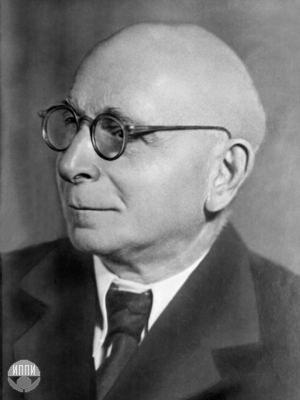
\includegraphics[width=.3\textwidth]{./fotos/calcasdos/Snbernstein.jpg}\\[5pt]

\includegraphics[width=.27\textwidth]{./fotos/calcasdos/Snbernstein.pdf}\\[5pt]
{\small \bfseries Sergei Bernstein}
\end{bio}

Se tiene el siguiente resultado.
\begin{theorem}[Bernstein]
  \label{teoaproxb}\index{teorema!de aproximación de Bernstein}Sea
  $f\colon[0,1]\rightarrow \mathbb{R}$ una función continua. La
  sucesión de polinomios de Bernstein $(\beta_{f,n})$ converge
  uniformemente a $f$ en $[0,1]$.
\end{theorem}

\begin{proof}
{\abovedisplayskip=9pt 
\belowdisplayskip=9pt 
  Sea $\varepsilon >0$. Como $f$ es uniformemente continua, existe
  $\delta >0$ tal que
  \begin{equation}
    \left\vert f(s)-f(t)\right\vert <\tfrac{\varepsilon }{2}\text{\qquad si }\left\vert s-t\right\vert <\delta .
    \label{conu}
  \end{equation}
  Fijemos $t\in [0,1]$. Multiplicando la igualdad (\ref{for1})
  por $f(t) $ obtenemos que
  \begin{equation*}
    f(t)=\sum_{k=0}^{n}f(t)\gamma_{n,k}(t)\text{\qquad }\forall n\in 
    \mathbb{N}.
  \end{equation*}
  En consecuencia,
  \begin{equation}
    \left\vert f(t)-\beta_{f,n}(t)\right\vert =\left\vert
      \sum_{k=0}^{n}\bigl(f(t)-f\bigl( \tfrac{k}{n}\bigr)\bigr)\gamma
     _{n,k}(t)\right\vert \leq \sum_{k=0}^{n}\left\vert f(t)-f\bigl( \tfrac{k}{n}\bigr) \right\vert \gamma_{n,k}(t).  \label{for9}
  \end{equation}
  Probaremos que el lado derecho de esta desigualdad es menor que
  $\varepsilon $ si $n$ satisface
  \begin{equation}
    n\geq \max \left\{ \frac{1}{\delta^{4}},\frac{\left\Vert f\right\Vert
       _{\infty }^{2}}{\varepsilon^{2}}\right\} .  \label{for5}
  \end{equation}

  Para ello consideremos los conjuntos
  \begin{align*}
    I_{1} &:=\Bigl\{ k\in \mathbb{N}\cup \left\{0\right\}:0\leq k\leq n,\text{ \ }\left\vert \tfrac{k}{n}-t\right\vert <\left( \tfrac{1}{n}\right)^{\frac{1}{4}}\Bigr\} , \\
    I_{2} &:=\bigl\{k\in \mathbb{N}\cup \left\{0\right\}:0\leq k\leq n,\text{ }k\notin
    I_{1}\bigr\},
  \end{align*}}%
  y tomemos una $n$ que cumpla (\ref{for5}). Entonces $\left(
    \frac{1}{n}\right)^{\frac{1}{4}}\leq \delta $, y se sigue de
  (\ref{conu}) y de (\ref{for1}) que
  \begin{equation}
    \sum_{k\in I_{1}}\left\vert f(t)-f\bigl( \tfrac{k}{n}\bigr) \right\vert
    \gamma_{n,k}(t)<\sum_{k\in I_{1}}\frac{\varepsilon }{2}\gamma_{n,k}(t)\leq 
    \frac{\varepsilon }{2}\sum_{k=0}^{n}\gamma_{n,k}(t)=\frac{\varepsilon }{2}.  \label{for8}
  \end{equation}
  Por otra parte, si $k\in I_{2}$ entonces $\bigl(t-\frac{k}{n}\bigr)^{-2}\leq
  \sqrt{n}$ \ y, en consecuencia,
  \begin{align}
    \sum_{k\in I_{2}}\left\vert f(t)-f\bigl( \tfrac{k}{n}\bigr) \right\vert
    \gamma_{n,k}(t) &\leq \sum_{k\in I_{2}}2\left\Vert f\right\Vert_{\infty
    }\gamma_{n,k}(t)  \notag \\
    &=2\left\Vert f\right\Vert_{\infty }\sum_{k\in I_{2}}\frac{\bigl(t-\frac{k}{n}\bigr)^{2}}{\bigl(t-\frac{k}{n}\bigr)^{2}}\gamma_{n,k}(t)  \notag \\
    &\leq 2\left\Vert f\right\Vert_{\infty }\sqrt{n}\sum_{k\in I_{2}}\bigl( t-\tfrac{k}{n}\bigr)^{2}\gamma_{n,k}(t).  \label{for7}
  \end{align}
  Probaremos ahora que
  \begin{equation}
    \sum_{k=0}^{n}\bigl( t-\tfrac{k}{n}\bigr)^{2}\gamma_{n,k}(t)\leq 
    \frac{1}{4n}\text{\qquad }\forall n\in \mathbb{N}.  \label{for4}
  \end{equation}
  Multiplicando la igualdad (\ref{for1}) por $t^{2}$, la igualdad
  (\ref{for2}) por $-\frac{2}{n}t$, y la suma de las igualdades
  (\ref{for2}) y (\ref{for3}) por $\frac{1}{n^{2}}$ obtenemos,
  respectivamente,
  \begin{align*}
    t^{2} &=\sum_{k=0}^{n}t^{2}\gamma_{n,k}(t), \\
    -2t^{2} &=\sum_{k=0}^{n}-2\tfrac{k}{n}t\gamma_{n,k}(t), \\
    \left( 1-\tfrac{1}{n}\right) t^{2}+\tfrac{1}{n}t &=\sum_{k=0}^{n}\tfrac{k^{2}}{n^{2}}\gamma_{n,k}(t).
  \end{align*}
  Sumando estas tres igualdades obtenemos
  \begin{equation}
    \frac{1}{n}(t-t^{2})=\sum_{k=0}^{n}\bigl( t-\tfrac{k}{n}\bigr)^{2}\gamma
   _{n,k}(t).  \label{for6}
  \end{equation}
  Observa que $\max_{t\in [0,1]}(t-t^{2})=\frac{1}{4}$. En
  consecuencia, (\ref{for6}) implica (\ref{for4}).

  Si $n$ satisface (\ref{for5}) entonces $\frac{\left\Vert
      f\right\Vert_{\infty }}{\sqrt{n}}\leq \varepsilon $. Por tanto,
  (\ref{for7}) y (\ref{for4}) implican que
  \begin{equation}
    \sum_{k\in I_{2}}\left\vert f(t)-f\bigl( \tfrac{k}{n}\bigr) \right\vert
    \gamma_{n,k}(t)\leq \frac{\varepsilon }{2}.  \label{for11}
  \end{equation}
  De las desigualdades (\ref{for9}), (\ref{for8}) y (\ref{for11})
  obtenemos que, si $n$ satisface (\ref{for5}), entonces
  \begin{align*}
    \left\vert f(t)-\beta_{f,n}(t)\right\vert &\leq \sum_{k=0}^{n}\left\vert
      f(t)-f\bigl( \tfrac{k}{n}\bigr) \right\vert \gamma_{n,k}(t) \\
    &=\sum_{k\in I_{1}}\left\vert f(t)-f\bigl( \tfrac{k}{n}\bigr) \right\vert
    \gamma_{n,k}(t)+\sum_{k\in I_{2}}\left\vert f(t)-f\bigl( \tfrac{k}{n}\bigr)
    \right\vert \gamma_{n,k}(t)<\varepsilon
  \end{align*}
  para toda $t\in [0,1]$. Es decir,
  \begin{equation}
    \left\Vert f-\beta_{f,n}\right\Vert_{\infty }<\varepsilon \text{\qquad si
      \ }n\geq \max \left\{ \frac{1}{\delta^{4}},\frac{\left\Vert f\right\Vert
       _{\infty }^{2}}{\varepsilon^{2}}\right\} .  \label{for10}
  \end{equation}
  Esto concluye la demostración.
\end{proof}

Observa que la fórmula (\ref{for10}) nos da una estimación del
error, en términos de $f$, en cada paso de la aproximación.

El siguiente resultado es consecuencia inmediata del teorema anterior.

\begin{theorem}[de aproximación de Weierstrass]
  \label{teoaproxw}\index{teorema!de aproximación de
    Weierstrass}Sea $f\colon[a,b]\rightarrow
  \mathbb{R}$ una función continua. Entonces existe una
  sucesión de polinomios $(p_{n})$ que converge uniformemente a
  $f$ en $[a,b]$.
\end{theorem}

\begin{proof}
  Este resultado se obtiene del anterior mediante un cambio de
  variable. Específicamente, sea $\rho \colon[0,1]\rightarrow [a,b]$ la función dada por $\rho (t):=(1-t)a+tb$. Aplicando el
  Teorema~\ref{teoaproxb} a la función $g:=f\circ \rho $ obtenemos
  que
  \begin{equation*}
    \beta_{g,n}\rightarrow g\text{\qquad en \ }\mathcal{C}^{0}[0,1].
  \end{equation*}
  La función $p_{n}:=\beta_{g,n}\circ \rho^{-1}$ es un polinomio
  y cumple que
  \begin{equation*}
    \left\Vert p_{n}-f\right\Vert_{\infty }=\max_{s\in [a,b]}\left\vert
      p_{n}(s)-f(s)\right\vert =\max_{t\in [0,1]}\left\vert \beta
     _{g,n}(t)-g(t)\right\vert =\left\Vert \beta_{g,n}-g\right\Vert_{\infty }.
  \end{equation*}
  En consecuencia, $p_{n}\rightarrow f$ en $\mathcal{C}^{0}[a,b]$.
\end{proof}

La compacidad del dominio de $f$ jugó un papel importante en la
demostración del Teorema~\ref{teoaproxb} para asegurar la
continuidad uniforme de $f$. El siguiente ejemplo muestra que el
Teorema~\ref{teoaproxw} no es válido, en general, si el dominio no
es compacto.

\begin{example}
  Sea $f(t)=\sen\frac{1}{t}$, $t\in (0,1]$. Ninguna sucesión
  de polinomios converge uniformemente a $f$ en $(0,1]$.
\begin{figure}[htb]
  \centering
  \begin{tikzpicture}[scale=0.9]
  \begin{axis}[ axis y line=left, axis x line=middle, ymin=-1.1, ymax=1.1,
    every inner x axis line/.append style={|-latex'},
    every inner y axis line/.append style={|-latex'},
    xticklabel style={/pgf/number format/frac, /pgf/number
      format/frac},
    xtick parsed={1/2, 1},
    yticklabel style={/pgf/number format/frac, /pgf/number
      format/frac},
    width=10cm,
    height=5cm
]
  \addplot[smooth, domain=0.02:1, thick, samples=5000]{sin(deg(1/x))};
\end{axis}

\end{tikzpicture}

  % \caption{}\label{fig:8.2}
\end{figure}
\end{example}

\begin{proof}
  Argumentando por contradicción, supongamos que existe una
  sucesión de polinomios $(p_{k})$ que converge uniformemente a
  $f$ en $(0,1]$. Entonces $(p_{k})$ converge a $f$ en
  $\mathcal{B}((0,1],\mathbb{R})$ (ver Proposición~\ref{convB=cu})
  y, por tanto, es de Cauchy en $\mathcal{B}((0,1],\mathbb{R})$. Es
  decir, dada $\varepsilon >0$ existe $k_{0}\in \mathbb{N}$ tal que
  \begin{equation*}
    \left\vert p_{k}(t)-p_{j}(t)\right\vert <\varepsilon \text{\qquad }\forall
    t\in \left( 0,1\right] \text{, \ }\forall k,j\geq k_{0}.
  \end{equation*}
  Como la función $t\mapsto \left\vert
    p_{k}(t)-p_{j}(t)\right\vert $ es continua en todo $\mathbb{R}$,
  la desigualdad anterior implica que
  \begin{equation*}
    \left\vert p_{k}(0)-p_{j}(0)\right\vert \leq \varepsilon \text{\qquad }\forall k,j\geq k_{0}.
  \end{equation*}
  Esto demuestra que $(p_{k})$ es de Cauchy en $\mathcal{C}^{0}[0,1]$.
  Por tanto, como $\mathcal{C}^{0}[0,1]$ es completo (ver
  Teorema~\ref{funcacotcompl}), existe $g\in \mathcal{C}^{0}[0,1]$ tal
  que
  \begin{equation*}
    p_{k}\rightarrow g\text{\qquad en \ }\mathcal{C}^{0}[0,1].
  \end{equation*}
  En particular, se cumple que
  \begin{equation*}
    g(t)=\lim_{k\rightarrow \infty }p_{k}(t)=\sen\tfrac{1}{t}\text{\qquad }\forall t\in (0,1].
  \end{equation*}
  Como $g$ es continua en $[0,1]$, se tiene entonces que
  \begin{equation*}
    \lim_{n\rightarrow \infty }\sen\tfrac{n\pi }{2}=\lim_{n\rightarrow
      \infty }g\left( \tfrac{2}{n\pi }\right) =g(0),
  \end{equation*}
  lo cual es una contradicción, ya que la sucesión $\left(
    \sen\frac{n\pi }{2}\right) $ no converge.
\end{proof}

\section{El teorema de Stone-Weierstrass}

Sea $X$ un espacio métrico.

\begin{definition}
  Un subconjunto $A$ de $X$ es \textbf{denso en} $X$ si $\
  \overline{A}=X$, \index{conjunto!denso}es decir, si para todo $x\in
  X$ existe una sucesión $(a_{k})$ en $A$ tal que
  $a_{k}\rightarrow x$ en $X$.
\end{definition}

Por ejemplo, el conjunto $\mathbb{Q}$ de los números racionales es
denso en $\mathbb{R}$.

Denotemos por $\mathbb{R}[t]$ al conjunto de todos los
polinomios
\begin{equation*}
  p\left( t\right) =\alpha_{0}+\alpha_{1}t+\cdots +\alpha_{n}t^{n},\text{\qquad }n\in \mathbb{N}\cup \left\{0\right\},\text{ \ }\alpha_{i}\in 
  \mathbb{R}\text{,}
\end{equation*}
con coeficientes reales. El Teorema~\ref{teoaproxw} afirma que el
conjunto de funciones polinomiales en $[a,b]$,
\begin{equation*}
  \mathcal{P}\left[ a,b\right] :=\left\{p\mid_{[a.b]}\,:p\in \mathbb{R}\!\left[ t\right] \right\},
\end{equation*}
es denso en $\mathcal{C}^{0}[a,b]$. En esta sección probaremos una
generalización de este resultado, conocido como el teorema de
Stone\footnote{Marshall Harvey Stone (1903-1989) nació en Nueva
  York. Estudió en la Universidad de Harvard, donde obtuvo el
  doctorado bajo la supervisión de George David Birkhoff. Fue
  profesor en esa universidad.}-Weierstrass.
\begin{bio}[H]
\centering
%
\includegraphics[width=.3\textwidth]{./fotos/calcasdos/Frechet.png}\\[5pt]

\includegraphics[width=.3\textwidth]{./fotos/calcasdos/Stone_3.pdf}\\[5pt]
{\small \bfseries Marshall Stone}
\end{bio}

Supondremos de aquí en adelante que $K$ es un espacio métrico
compacto y, por simplicidad, denotaremos por 
\index{espacio!C ala0K@$\mathcal{C}^{0}(K)$}
\begin{equation*}
  \mathcal{C}^{0}(K):=\mathcal{C}^{0}(K,\mathbb{R})
\end{equation*}
al espacio de funciones continuas $f\colon K\rightarrow \mathbb{R}$ con la
norma uniforme
\begin{equation*}
  \left\Vert f\right\Vert_{\infty }=\max_{x\in K}\left\vert f(x)\right\vert .
\end{equation*}
Observa que $\mathcal{C}^{0}(K)$ no sólo es un espacio vectorial
sino que cuenta además con un producto, definido como sigue:
\begin{equation*}
  fg\colon K\rightarrow \mathbb{R},\text{\qquad }(fg)(x):=f(x)g(x).
\end{equation*}
Este producto le da al espacio vectorial $\mathcal{C}^{0}(K)$ la
estructura de una $\mathbb{R}$-álgebra con unidad [Ejercicio
\ref{algebra}]. La unidad es la función constante igual a $1$, a
la que denotamos por $1$.

El siguiente resultado da condiciones suficientes para que un
subconjunto $\mathcal{A}$ de $\mathcal{C}^{0}(K)$ sea denso en
$\mathcal{C}^{0}(K)$.

\begin{theorem}[Stone-Weierstrass]
  \label{teosw}\index{teorema!de Stone-Weierstrass}Sea $K$ un espacio
  métrico compacto y sea $\mathcal{A}$ un subconjunto de
  $\mathcal{C}^{0}(K)$\ con las siguientes propiedades:

  \begin{enumerate}
  \item[(a)] $\lambda \varphi +\mu \psi \in \mathcal{A}$\quad para
    cualesquiera $\ \varphi ,\psi \in \mathcal{A}$ y $\lambda ,\mu \in
    \mathbb{R} $.

  \item[(b)] $\varphi \psi \in \mathcal{A}$\quad para cualesquiera
    $\varphi ,\psi \in \mathcal{A}$.

  \item[(c)] $1\in \mathcal{A}$.

  \item[(d)] Dados $x_{1}\neq x_{2}$ en $K$, existe $\varphi \in
    \mathcal{A}$ tal que $\varphi (x_{1})\neq \varphi (x_{2})$.
  \end{enumerate}

  Entonces $\mathcal{A}$ es denso en $\mathcal{C}^{0}(K)$, es decir,
  dada una función continua $f\colon K\rightarrow \mathbb{R}$ existe una
  sucesión $(\varphi_{k})$ de funciones en $\mathcal{A}$ que
  converge uniformemente a $f $ en $K$.
\end{theorem}

En términos algebraicos, las primeras tres condiciones \emph{(a),
  (b)} y \emph{(c)} se expresan diciendo que $\mathcal{A}$ \emph{es
  una} $\mathbb{R}$\emph{-subálgebra con unidad de la
}$\mathbb{R}$\emph{-álgebra de funciones continuas}
$\mathcal{C}^{0}(K)$. La propiedad \emph{(d)} suele expresarse
diciendo que $\mathcal{A}$ \emph{separa puntos}.

Para demostrar el teorema de Stone-Weierstrass usaremos los siguientes
cuatro lemas.

\begin{lemma}
  \label{lemsw1}Dados $x_{1}\neq x_{2}$ en $K$ \ y\ $\ c_{1},c_{2}\in
  \mathbb{R}$, existe $\psi \in \mathcal{A}$ tal que $\psi
  (x_{1})=c_{1}$ y $\psi (x_{2})=c_{2}$.
\end{lemma}

\begin{proof}
  Sea $\varphi \in \mathcal{A}$ tal que $\varphi (x_{1})\neq \varphi
  (x_{2})$. Como el determinante
  \begin{equation*}
      \begin{vmatrix}
        \varphi (x_{1}) & 1 \\ 
        \varphi (x_{2}) & 1
      \end{vmatrix}
      \neq 0,
  \end{equation*}
  existen $\lambda ,\mu \in \mathbb{R}$ tales que
  \begin{align}
    \lambda \varphi (x_{1})+\mu &=c_{1}  \label{c1} \\
    \lambda \varphi (x_{2})+\mu &=c_{2}  \label{c2}
  \end{align}
  De las propiedades \emph{(a)} y \emph{(c)} se sigue que la
  función $\psi :=\lambda \varphi +\mu 1\in \mathcal{A}$. Las
  igualdades (\ref{c1}) y (\ref{c2}) afirman que $\psi (x_{1})=c_{1}$
  y $\psi (x_{2})=c_{2}$.
\end{proof}

\begin{lemma}
  \label{lemsw2}La cerradura $\overline{\mathcal{A}}$\ de
  $\mathcal{A}$\ en $\mathcal{C}^{0}(K)$ también tiene las
  propiedades (a), (b) y\ (c).
\end{lemma}

\begin{proof}
  Es sencillo comprobar que $\overline{\mathcal{A}}$ tiene la
  propiedad \emph{(a)} [Ejercicio~\ref{cerrev}]. La propiedad
  \emph{(c)} es inmediata.  Probemos \emph{(b)}\textsl{. }Dadas
  $\varphi ,\psi \in \overline{\mathcal{A}} $ existen $\varphi
 _{k},\psi_{k}\in \mathcal{A}$ tales que $\varphi_{k}\rightarrow
  \varphi $ y $\psi_{k}\rightarrow \psi $ en $\mathcal{C}^{0}(K)$
  (ver Proposición~\ref{cerrsuc}). Como toda sucesión
  convergente está acotada, existe $C>0$ tal que $\left\Vert \psi
   _{k}\right\Vert_{\infty }\leq C$ para toda $k$. En consecuencia,
  \begin{align*}
    \left\Vert \varphi \psi -\varphi_{k}\psi_{k}\right\Vert_{\infty } &\leq
    \left\Vert \varphi (\psi -\psi_{k})\right\Vert_{\infty }+\left\Vert
      (\varphi -\varphi_{k})\psi_{k}\right\Vert_{\infty } \\[5pt]
    &\leq \left\Vert \varphi \right\Vert_{\infty }\left\Vert (\psi -\psi
     _{k})\right\Vert_{\infty }+\left\Vert (\varphi -\varphi_{k})\right\Vert
   _{\infty }\left\Vert \psi_{k}\right\Vert_{\infty } \\[5pt]
    &\leq \left\Vert \varphi \right\Vert_{\infty }\left\Vert (\psi -\psi
     _{k})\right\Vert_{\infty }+C\left\Vert (\varphi -\varphi_{k})\right\Vert
   _{\infty }.
  \end{align*}
  Tomando el límite cuando $k\rightarrow \infty $ en ambos lados
  de la desigualdad obtenemos que $\varphi_{k}\psi_{k}\rightarrow
  \varphi \psi $.  Dado que $\varphi_{k}\psi_{k}\in \mathcal{A}$,
  concluimos que $\varphi \psi \in \overline{\mathcal{A}}$ (ver
  Proposición~\ref{cerrsuc}).
\end{proof}

\begin{lemma}
  \label{lemsw3}Si $\varphi \in \overline{\mathcal{A}}$, entonces
  $\left\vert \varphi \right\vert \in \overline{\mathcal{A}}$.
\end{lemma}

\begin{proof}
  Como $\varphi $ es continua y $K$ es compacto, se tiene que
  $\varphi (K)$ es acotado en $\mathbb{R}$ (ver
  Corolario~\ref{contencomp}). Por tanto, $\varphi (K)$ está contenido
  en algún intervalo $[a,b]$. Por el Teorema~\ref{teoaproxw} existe
  una sucesión de polinomios $p_{k}$ que converge uniformemente a la
  función valor absoluto $\left\vert \cdot \right\vert $ en el
  intervalo $[a,b]$, es decir, dada $\varepsilon >0$ existe
  $k_{0}\in \mathbb{N}$ tal que
  \begin{equation*}
    \left\vert p_{k}(t)-\left\vert t\right\vert \right\vert <\varepsilon \text{\qquad }\forall k\geq k_{0}\text{ \ }\forall t\in [a,b].
  \end{equation*}
  Esta desigualdad se cumple, en particular, para $t=\varphi (x)$ con
  $x\in K$. Por tanto,
  \begin{equation*}
    \left\Vert p_{k}\circ \varphi -\left\vert \varphi \right\vert \right\Vert
   _{\infty }=\max_{x\in K}\left\vert p_{k}(\varphi (x))-\left\vert \varphi
        (x)\right\vert \right\vert <\varepsilon \text{\qquad }\forall k\geq k_{0},
  \end{equation*}
  es decir, $p_{k}\circ \varphi \rightarrow \left\vert \varphi
  \right\vert $ en $\mathcal{C}^{0}(K)$.

  Por otra parte, el Lema~\ref{lemsw2} asegura que, para cualquier
  polinomio $p(t)=\alpha_{0}+\alpha_{1}t+\cdots +\alpha_{m}t^{m}$,
  se cumple que
  \begin{equation*}
    p\circ \varphi =\alpha_{0}+\alpha_{1}\varphi +\cdots +\alpha_{m}\varphi
   ^{m}\in \overline{\mathcal{A}}.
  \end{equation*}
  Por tanto, $\left\vert \varphi \right\vert \in
  \overline{\mathcal{A}}$.
\end{proof}

Dadas dos funciones $f,g\colon K\rightarrow \mathbb{R}$ denotamos por $\max
\left\{f,g\right\}$, $\min \left\{f,g\right\}\colon K\rightarrow \mathbb{R}$ a las funciones
\begin{equation*}
  (\max \left\{f,g\right\})(x):=\max \left\{f(x),g(x)\right\},\text{\qquad }(\min \left\{f,g\right\})(x):=\min
  \left\{f(x),g(x)\right\}.
\end{equation*}
%\pagebreak
\begin{lemma}
  \label{lemsw4}Si $\varphi ,\psi \in \overline{\mathcal{A}}$.
  entonces $\ \max \left\{\varphi ,\psi \right\},\min \left\{\varphi ,\psi \right\}\in
  \overline{\mathcal{A}}$.
\end{lemma}

\begin{proof}
  Basta observar que
  \begin{align}
    \max \left\{\varphi ,\psi \right\} &=\frac{1}{2}\left( \varphi +\psi +\left\vert
        \varphi -\psi \right\vert \right)  \label{idmax} \\
    \min \left\{\varphi ,\psi \right\} &=\frac{1}{2}\left( \varphi +\psi -\left\vert
        \varphi -\psi \right\vert \right)  \label{idmin}
  \end{align}
  Como $\overline{\mathcal{A}}$ satisface la propiedad \emph{(a)}, el
  lema anterior implica que $\max \left\{\varphi ,\psi \right\},\min \left\{\varphi
  ,\psi \right\}\in \overline{\mathcal{A}}$.
\end{proof}

%\medskip

\begin{proof}[Demostración del Teorema~\ref{teosw}.]
%\textbf{Demostración del Teorema~\ref{teosw}.\qquad }
Sea
$f\colon K\rightarrow \mathbb{R}$ una función continua y sea
$\varepsilon >0$. El Lema~\ref{lemsw1} asegura que, para cada par de
puntos $x,y\in K$, podemos escoger $\varphi_{x,y}\in \mathcal{A}$ tal
que $\varphi_{x,y}(x)=f(x)$ y $\varphi_{x,y}(y)=f(y)$.

Fijemos $x\in K$. Como $\varphi_{x,y}-f$ es continua y $\varphi
_{x,y}(y)-f(y)=0$, existe $\delta_{y}>0$ tal que
\begin{equation}
  \left\vert \varphi_{x,y}(z)-f(z)\right\vert <\varepsilon \text{\qquad }\forall z\in B_{K}(y,\delta_{y})  \label{sw0}
\end{equation}
y, como $K$ es compacto, existen $y_{1},\dots,y_{m}\in K$ tales que
\begin{equation*}
  K\subset B_{K}(y_{1},\delta_{y_{1}})\cup \cdots \cup B_{K}(y_{m},\delta
 _{y_{m}}).
\end{equation*}
Sea $\varphi_{x}:=\max \left\{\varphi_{x,y_{1}},\dots,\varphi
_{x,y_{m}}\right\}$. El Lema~\ref{lemsw4} asegura que $\varphi_{x}\in
\overline{\mathcal{A}}$. Puesto que cada $z\in K$ pertenece a alguna
$B(y_{i},\delta_{y_{i}})$, la desigualdad (\ref{sw0}) implica que
\begin{equation}
  \varphi_{x}(z)-f(z)>-\varepsilon \text{\qquad }\forall z\in K.  \label{sw1}
\end{equation}

Por otra parte, dado que $\varphi_{x,y}(x)=f(x)$ para todo $y\in K$,
se tiene que $\varphi_{x}(x)=f(x)$ y, como $\varphi_{x}-f$ es
continua, existe $\gamma_{x}>0$ tal que
\begin{equation}
  \left\vert \varphi_{x}(z)-f(z)\right\vert <\varepsilon \text{\qquad }\forall z\in B_{K}(x,\gamma_{x}).  \label{sw00}
\end{equation}
De la compacidad de $K$ se sigue que existen $x_{1},\dots,x_{n}\in K$
tales que
\begin{equation*}
  K\subset B_{K}(x_{1},\gamma_{x_{1}})\cup \cdots \cup B_{K}(x_{n},\gamma
 _{x_{n}}).
\end{equation*}
Sea $\varphi :=\min \left\{\varphi_{x_{1}},\dots,\varphi_{x_{n}}\right\}$. El
Lema~\ref{lemsw4} asegura que $\varphi \in \overline{\mathcal{A}}$.
Puesto que cada $z\in K$ pertenece a alguna $B(x_{i},\gamma
_{x_{i}})$, usando la desigualdad (\ref{sw00}) obtenemos que
\begin{equation}
  \varphi (z)-f(z)<\varepsilon \text{\qquad }\forall z\in K.  \label{sw2}
\end{equation}
Y, como la desigualdad (\ref{sw1}) vale para toda $x\in K$, se tiene
además que
\begin{equation}
  \varphi (z)-f(z)>-\varepsilon \text{\qquad }\forall z\in K.  \label{sw3}
\end{equation}
Las desigualdades (\ref{sw2}) y (\ref{sw3}) implican que $\left\Vert
  \varphi -f\right\Vert_{\infty }<\varepsilon $. Por consiguiente,
dado que $\varphi \in \overline{\mathcal{A}}$, concluimos que $f\in
\overline{\mathcal{A}}$.
\end{proof}
%\medskip

Denotemos por $\mathbb{R}[ x_{1},\dots,x_{n}] $ al conjunto
de polinomios
\begin{equation*}
  p(x_{1},\dots,x_{n})=\sum_{i=1}^{m}a_{i}x_{1}^{k_{i,1}}\cdots
  x_{n}^{k_{i,n}},\text{\qquad }a_{i}\in \mathbb{R},\text{\quad }k_{i,j}\in 
  \mathbb{N}\cup \left\{0\right\},
\end{equation*}
en $n$ variables con coeficientes reales. Una consecuencia interesante
del teorema de Stone-Weierstrass es la siguiente.

\begin{corollary}
  \label{aproxpoli}Sea $K$ un subconjunto compacto de
  $\mathbb{R}^{n}$. Entonces, dada una función continua
  $f\colon K\rightarrow \mathbb{R}$, existe una sucesión de polinomios
  $\left( p_{k}\right) $ en $\mathbb{R}[ x_{1},\dots,x_{n}] $
  que converge uniformemente a $f$ en $K$.
\end{corollary}

\begin{proof}
  Obviamente el conjunto
  \begin{equation*}
    \mathcal{P}(K):=\left\{p\mid_{K}\,:p\in \mathbb{R}[ x_{1},\dots,x_{n}]
    \right\}
  \end{equation*}
  satisface las condiciones \emph{(a), (b) }y \emph{(c)} del
  Teorema~\ref{teosw}.

  Consideremos los polinomios $\pi_{i}(x_{1},\dots,x_{n})=x_{i}$,
  $i=1,\dots,n$. Si $\xi ,\eta \in K$ son puntos distintos, entonces al
  menos una de sus coordenadas es distinta, digamos que $\xi_{i}\neq
  \eta_{i}$. Entonces, $\pi_{i}(\xi )=\xi_{i}\neq \eta_{i}=\pi
 _{i}(\eta )$. Esto prueba que $\mathcal{P}(K)$ satisface la
  condición \emph{(d). }

  El Teorema~\ref{teosw} asegura entonces que existe una sucesión
  de polinomios $\left( p_{k}\right) $ en $\mathbb{R}[
    x_{1},\dots,x_{n}]$ que converge uniformemente a $f$ en $K$.
\end{proof}

\section{Ejercicios}

\begin{exercise}
  \label{ejfor3}Demuestra la igualdad \emph{(\ref{for3})}.
\end{exercise}

\begin{exercise}
  \label{trans}Sea $X$ un espacio métrico. Prueba que, si
  $Z\subset Y\subset X$ y $Z$ es denso en $X$, entonces $Y$ es denso
  en $X$.
\end{exercise}

\begin{exercise}
  \label{imdens}Prueba que, si $\phi \colon X\rightarrow Y$ es continua y
  suprayectiva y $A$ es denso en $X$, entonces $\phi (A)$ es denso en
  $Y$.
\end{exercise}

\begin{exercise}
  Prueba que el conjunto
  \begin{equation*}
    \mathbb{Q}^{n}:=\left\{(q_{1},\dots,q_{n})\in \mathbb{R}^{n}:q_{k}\in \mathbb{Q}\text{ \ }\forall k=1,\dots,n\right\}
  \end{equation*}
  es denso en $\mathbb{R}^{n}$.
\end{exercise}

\begin{exercise}
  Sea $\mathbb{Q}^{\infty }$ el conjunto de todas las sucesiones
  $(q_{1},\dots,q_{k},0,0,\dots)$ de números racionales tales que
  sólo un número finito de sus términos es distinto de
  cero.

  \begin{enumerate}
  \item[(a)] Prueba que $\mathbb{Q}^{\infty }$ es denso en $\ell_{p}$
    para todo $p\in [1,\infty )$.

  \item[(b)] ¿Es $\mathbb{Q}^{\infty }$ denso en
    $\ell_{\infty }$?
  \end{enumerate}
\end{exercise}

\begin{exercise}
  Sea $\mathbb{Q}[ t]$ el conjunto de todos los polinomios
  \begin{equation*}
    q\left( t\right) =q_{0}+q_{1}t+\cdots +q_{n}t^{n},\text{ \ }n\in \mathbb{N}\cup \left\{0\right\},\text{ }q_{i}\in \mathbb{Q}\text{,}
  \end{equation*}
  con coeficientes racionales. Prueba que
  \begin{equation*}
    \mathcal{P}_{\mathbb{Q}}[ a,b] :=\left\{q\mid_{[a,b]}\,:q\in 
    \mathbb{Q}[ t] \right\}
  \end{equation*}
  es denso en $\mathcal{C}^{0}[a,b]$.
\end{exercise}

\begin{exercise}
  \label{nonum}Se dice que un conjunto $A$ es \textbf{a lo más
    numerable} \index{conjunto!a lo más numerable}si existe una
  función inyectiva $i\colon A\rightarrow \mathbb{N}$. Demuestra las
  siguientes afirmaciones:

  \begin{enumerate}
  \item[(a)] El conjunto $\mathbb{Q}$ de los números racionales es
    a lo más numerable.

  \item[(b)] El conjunto de todas las sucesiones $(b_{k})$\ tales que
    $b_{k}\in \left\{0,1\right\}$\ no es a lo más numerable.

  \item[(c)] Prueba que $\mathbb{R}$ no es a lo más
    numerable. \emph{(Sugerencia: Usa el hecho de que todo número
      real tiene una representación binaria.)}
  \end{enumerate}
\end{exercise}

\begin{exercise}
  Un espacio métrico $X$ se llama \textbf{separable}
  \index{espacio!separable}si contiene un subconjunto a lo más
  numerable que es denso en $X$. Demuestra las siguientes
  afirmaciones:

  \begin{enumerate}
  \item[(a)] Ningún subconjunto propio de un espacio métrico
    discreto $X_{\disc}$ es denso en $X_{\disc}$.

  \item[(b)] Un espacio métrico discreto $X_{\disc}$ es separable
    si y sólo si $X_{\disc}$ es a lo más numerable.
  \end{enumerate}
\end{exercise}

\pagebreak

\begin{exercise}
  Investiga si los siguientes espacios métricos son o no
  separables.

  \begin{enumerate}
  \item[(a)] $\mathbb{R}_{p}^{n}$ \ con $p\in [1,\infty ]$.

  \item[(b)] $\ell_{p}$ \ con $p\in [1,\infty ]$.

  \item[(c)] $\mathcal{C}_{p}^{0}[a,b]$ \ con $p\in [1,\infty
    ]$.

  \item[(d)] $\mathcal{C}_{b}^{0}(\mathbb{R},\mathbb{R})$.
  \end{enumerate}
\end{exercise}

\begin{exercise}
  Prueba que todo espacio métrico compacto $X$ es
  separable. \emph{(Sugerencia: Para cada }$k\in \mathbb{N}$,
  \emph{toma un conjunto finito de bolas de radio
  }$\frac{1}{k}$\emph{\ cuya unión es }$X$.\emph{\ Considera el
    conjunto de centros de todas esas bolas.)}
\end{exercise}

\begin{exercise}
  Sea $\Omega $ un subconjunto abierto y acotado de $\mathbb{R}^{n}$.
  Denotemos por $\mathcal{C}^{\infty }(\overline{\Omega })$ al
  conjunto de todas las funciones
  $f\colon\Omega \rightarrow \mathbb{R}$ que tienen derivadas
  parciales de todos los órdenes en $\Omega $ y dichas derivadas
  tienen una extensión continua a la cerradura de $\Omega $. Prueba
  que $\mathcal{C}^{\infty }(\overline{\Omega })$ es denso en
  $\mathcal{C}^{0}(\overline{\Omega })$.  \emph{(Sugerencia: Usa el
    Corolario~\ref{aproxpoli} y el Ejercicio~\ref{trans}.)}
\end{exercise}

\begin{exercise}
  Sea $f\in \mathcal{C}^{0}[0,1]$ tal que
  \begin{equation*}
    \int_{0}^{1}f(x)x^{n}dx=0\text{\qquad }\forall n\in \mathbb{N}\cup \left\{0\right\}.
  \end{equation*}
  Prueba que
  \begin{equation*}
    \int_{0}^{1}f^{2}(x)dx=0
  \end{equation*}
  y concluye que $f(x)=0$ para todo $x\in [0,1]$.
\end{exercise}

\begin{exercise}
  Sea $\mathbb{S}^{1}=\left\{(\cos \theta ,\sen \theta )\in
  \mathbb{R}^{2}:0\leq \theta \leq 2\pi \right\}$ el círculo unitario
  en $\mathbb{R}^{2}$. Prueba que cualquier función continua
  $f\colon\mathbb{S}^{1}\rightarrow \mathbb{R}$ es el límite uniforme
  de funciones de la forma
  \begin{equation*}
    \varphi (\cos \theta ,\sen \theta )=a_{0}+a_{1}\cos \theta +b_{1}\sen \theta
    +\cdots +a_{n}\cos n\theta +b_{n}\sen n\theta
  \end{equation*}
  con $a_{i},b_{i}\in \mathbb{R}$, $n\in \mathbb{N}\cup \left\{0\right\}$.
\end{exercise}

\begin{exercise}
  Sean $X$ y $Y$ espacios métricos compactos. Prueba que cualquier
  función continua $f\colon X\times Y\rightarrow \mathbb{R}$ es el
  límite uniforme de funciones de la forma
  \begin{equation*}
    \varphi (x,y)=f_{1}(x)g_{1}(y)+\cdots +f_{n}(x)g_{n}(y),
  \end{equation*}
  con $f_{1},\dots,f_{n}\in \mathcal{C}^{0}(X)$, $g_{1},\dots,g_{n}\in
  \mathcal{C}^{0}(Y)$ y $n\in \mathbb{N}$.
\end{exercise}

\begin{exercise}
  \label{algebra}Investiga lo que es una $\mathbb{R}$-álgebra con
  unidad\ y prueba que, para cualquier espacio métrico $X$, el
  espacio $\mathcal{C}^{0}(X)$ es una $\mathbb{R}$-álgebra con
  unidad.
\end{exercise}

\begin{exercise}
  \label{cerrev}Sea $\mathcal{A}$ un subespacio vectorial de
  $\mathcal{C}^{0}(X)$.\ Prueba que $\overline{\mathcal{A}}$ es un
  subespacio vectorial de $\mathcal{C}^{0}(X)$. \emph{(Sugerencia: Usa
    el Ejercicio~\ref{contopev}.)}
\end{exercise}

\part{Diferenciabilidad}

\chapter{Diferenciabilidad}

El cálculo diferencial estudia las funciones
$f\colon \mathbb{R}^{n}\rightarrow \mathbb{R}^{m}$ que se pueden aproximar
localmente por una función lineal. La derivada de $f$ en un punto
$x_{0}$ de $\mathbb{R}^{n} $ es la función lineal $f^{\prime
}(x_{0})\colon \mathbb{R}^{n}\rightarrow \mathbb{R}^{m}$ que mejor aproxima
a $f$ en dicho punto, en el sentido de que la distancia entre $\
f(x_{0}+x)$ \ y $\ f(x_{0})+f^{\prime }(x_{0})x$ \ tiende a cero
más rápidamente que $x$. Dicho de modo preciso,
\begin{equation*}
  \lim_{x\rightarrow 0}\frac{\left\Vert f(x_{0}+x)-\left( f(x_{0})+f^{\prime
        }(x_{0})x\right) \right\Vert }{\left\Vert x\right\Vert }=0.
\end{equation*}
Las funciones que admiten tal aproximación se llaman
diferenciables.

La noción de diferenciabilidad se extiende de manera natural a
funciones $f\colon V\rightarrow W$ entre espacios de Banach con la siguiente
precaución: además de requerir que $f^{\prime
}(x_{0})\colon V\rightarrow W$ sea una función lineal es necesario pedir
que sea continua. Recuerda que las funciones lineales entre espacios
de Banach de dimensión infinita no son necesariamente
continuas. La continuidad de $f^{\prime }(x_{0})$ juega un papel
esencial para la validez de muchas propiedades importantes, como la
continuidad de las funciones diferenciables o la regla de la
cadena. El papel de la continuidad queda oculto cuando consideramos
funciones entre espacios euclidianos: la usamos sin darnos cuenta,
pues toda función lineal entre espacios de dimensión finita es
automáticamente continua.

En este capítulo introduciremos el concepto de derivada para funciones
entre espacios de Banach y estudiaremos sus propiedades
fundamentales. Los resultados que presentaremos son generalizaciones
inmediatas de los resultados de cálculo que ya conocemos. Sin embargo,
presentarlos en esta generalidad tiene varias ventajas. Por una parte,
hay aplicaciones importantes que requieren este nivel de
generalidad. Por ejemplo, las soluciones de muchas ecuaciones
diferenciales parciales, que modelan problemas importantes de la
física, la ingeniería, la biología y otras disciplinas, resultan ser
puntos críticos de una función diferenciable definida en un espacio de
funciones\footnote{Consulta, por ejemplo,~\cite{Costa}.}.

Por otra parte, este nivel de generalidad permite definir muchos
conceptos de manera sencilla. Un ejemplo de ello son las derivadas de
orden superior, cada una de las cuales no es sino la derivada de la
precedente. Además, la demostración en esta generalidad de los
resultados que ya conocemos ayuda a comprenderlos mejor y a mayor
profundidad. Y no perdemos nada, ya que las demostraciones no son ni
más largas ni más complicadas que las correspondientes para
espacios euclidianos.

\section{El espacio de funciones lineales y continuas}

\label{funclincont}Empezaremos estudiando al espacio de las funciones
lineales y continuas entre dos espacios de Banach $V=(V,\left\Vert
  \cdot \right\Vert_{V})$ y $W=(W,\left\Vert \cdot \right\Vert
_{W})$.

La continuidad de una función lineal entre ellos se caracteriza
como sigue.

\begin{proposition}
  \label{lin+cont}Si $T\colon V\rightarrow W$ es una función lineal, son
  equivalentes las siguientes afirmaciones:

  \begin{enumerate}
  \item[(a)] $T$ es continua

  \item[(b)] $T$ es continua en $0$.

  \item[(c)] Existe $c\in \mathbb{R}$ tal que $\ \left\Vert
      Tv\right\Vert_{W}\leq c\left\Vert v\right\Vert_{V}$ \ para
    todo\ $v\in V$.

  \item[(d)] $T$ es Lipschitz continua.
  \end{enumerate}
\end{proposition}

\begin{proof}
  Las implicaciones \emph{(a)}$\Rightarrow $\emph{(b)} y
  \emph{(d)}$\Rightarrow $\emph{(a)} son evidentes.

  \emph{(b)}$\Rightarrow $\emph{(c)}: Si $T$ es continua en $0$
  existe $\delta >0$ tal que
  \begin{equation*}
    \left\Vert Tv\right\Vert_{W}<1\text{\qquad si }\left\Vert v\right\Vert
   _{V}<\delta .
  \end{equation*}
  En consecuencia,
  \begin{equation*}
    \left\Vert Tv\right\Vert_{W}=\frac{2}{\delta }\left\Vert v\right\Vert
   _{V}\left\Vert T\left( \frac{\delta }{2}\frac{v}{\left\Vert v\right\Vert_{V}}\right) \right\Vert_{W}<\frac{2}{\delta }\left\Vert v\right\Vert_{V}\text{\qquad }\forall v\in V.
  \end{equation*}

  \emph{(c)}$\Rightarrow $\emph{(d)}: Si existe $c>0$ tal que $\
  \left\Vert Tv\right\Vert_{W}\leq c\left\Vert v\right\Vert_{V}$ \
  para todo\ $v\in V$, entonces
  \begin{equation*}
    \left\Vert Tv_{1}-Tv_{2}\right\Vert_{W}=\left\Vert
      T(v_{1}-v_{2})\right\Vert_{W}\leq c\left\Vert v_{1}-v_{2}\right\Vert_{V}\text{\qquad }\forall v_{1},v_{2}\in V.
  \end{equation*}
  Esto prueba que $T$ es Lipschitz continua.
\end{proof}

\begin{definition}
  Denotamos por\index{espacio!L (VW)@$\mathcal{L}(V,W)$}
  \begin{equation*}
    \mathcal{L}(V,W):=\left\{T\colon V\rightarrow W:T\text{ es lineal y continua}\right\}
  \end{equation*}
  y definimos
  \begin{equation}
    \left\Vert T\right\Vert_{\mathcal{L}(V,W)}:=\sup_{\substack{ v\in V  \\ v\neq 0}}\frac{\left\Vert Tv\right\Vert_{W}}{\left\Vert v\right\Vert_{V}}\text{\qquad }\forall T\in \mathcal{L}(V,W).  \label{defnorma}
  \end{equation}
\end{definition}

Nota que $\mathcal{L}(V,W)$ es un espacio vectorial con las
operaciones dadas por
\begin{equation*}
  (T+S)v:=Tv+Sv,\text{\qquad }(\lambda T)v:=\lambda Tv,
\end{equation*}
donde $T,S\in \mathcal{L}(V,W)$, $\lambda \in \mathbb{R}$ y $v\in V$.
La Proposición~\ref{lin+cont}\ asegura que $\left\Vert
  T\right\Vert_{\mathcal{L}(V,W)}<\infty $. Es sencillo comprobar que
$\left\Vert \cdot \right\Vert_{\mathcal{L}(V,W)}$ es una norma en
$\mathcal{L}(V,W)$ [Ejercicio~\ref{norma}].

Observa que
\begin{equation}
  \left\Vert Tv\right\Vert_{W}\leq \left\Vert T\right\Vert_{\mathcal{L}(V,W)}\left\Vert v\right\Vert_{V}\text{\qquad }\forall v\in V,\text{ \ }\forall T\in \mathcal{L}(V,W).  \label{opernorm}
\end{equation}
Usaremos con frecuencia esta desigualdad.

\begin{proposition}
  \label{lin+contBanach}$\mathcal{L}(V,W)$ con la norma definida en
  \emph{(\ref{defnorma})}\ es un espacio de Banach.
\end{proposition}

\begin{proof}
  Sean $(T_{k})$ una sucesión de Cauchy en $\mathcal{L}(V,W)$ y
  $\varepsilon >0$. Entonces existe $k_{0}\in \mathbb{N}$ tal que
  \begin{equation*}
    \left\Vert T_{k}-T_{j}\right\Vert_{\mathcal{L}(V,W)}<\varepsilon \text{\qquad }\forall j,k\geq k_{0}.
  \end{equation*}
  Por tanto,
  \begin{equation}
    \bigl\Vert T_{k}v-T_{j}v\bigr\Vert_{W}\leq\varepsilon \bigl\Vert v\bigr\Vert
   _{V}\text{\qquad }\forall j,k\geq k_{0},\text{ \ }\forall v\in V.
    \label{punc}
  \end{equation}
  Esto implica que, para cada $v\in V$, la sucesión $(T_{k}v)$ es
  de Cauchy en $W$ y, como $W$ es un espacio de Banach, existe $Tv\in
  W$ tal que
  \begin{equation*}
    T_{k}v\rightarrow Tv\text{\qquad en \ }W.
  \end{equation*}
  Probaremos primero que $T\in \mathcal{L}(V,W)$.

  Si $v,w\in V$, $\lambda ,\mu \in \mathbb{R}$, se tiene que
  \begin{align*}
    T(\lambda v+\mu w) &=\lim_{k\rightarrow \infty }T_{k}(\lambda v+\mu
    w)=\lim_{k\rightarrow \infty }(\lambda T_{k}v+\mu T_{k}w) \\
    &=\lambda \lim_{k\rightarrow \infty }T_{k}v+\mu \lim_{k\rightarrow \infty
    }T_{k}w=\lambda Tv+\mu Tw.
  \end{align*}
  Esto prueba que $T$ es lineal. Por otra parte, haciendo tender
  $k\rightarrow \infty $ en la desigualdad (\ref{punc}) obtenemos
  \begin{equation}
    \bigl\Vert Tv-T_{j}v\bigr\Vert_{W}\leq \varepsilon \bigl\Vert v\bigr\Vert
   _{V}\qquad\forall j\geq k_{0},\quad\forall v\in V.
    \label{limpunc}
  \end{equation}
  De la Proposición~\ref{lin+cont} se sigue que $T-T_{k_{0}}$ es
  continua.  Por tanto, $T=(T-T_{k_{0}})+T_{k_{0}}$ es continua.

  Finalmente, la desigualdad (\ref{limpunc}) implica que
  \begin{equation*}
    \frac{\left\Vert Tv-T_{j}v\right\Vert_{W}}{\bigl\Vert
        v\bigr\Vert_{V}}\leq \varepsilon 
    \qquad\forall j\geq k_{0},\quad\forall v\in V,\; v\neq0.
  \end{equation*}
  Por tanto,
  \begin{equation*}
    \left\Vert T-T_{j}\right\Vert_{\mathcal{L}(V,W)}\leq \varepsilon\qquad\forall j\geq k_{0}.
  \end{equation*}
  Esto prueba que $T_{j}\rightarrow T$ en $\mathcal{L}(V,W)$. En
  consecuencia, $\mathcal{L}(V,W)$ es un espacio de Banach.
\end{proof}

Recuerda que, si $\dim V<\infty $, cualquier función lineal
$T\colon V\rightarrow W$ es continua (ver Ejercicio~\ref{ejnorfinequiv}), de
modo que $\mathcal{L}(V,W)$ es simplemente el espacio de funciones
lineales de $V$ a $W$. En particular,
$\mathcal{L}(\mathbb{R}^{n},\mathbb{R}^{m})$ es isomorfo a
$\mathbb{R}^{mn}$ y cualquier isomorfismo resulta ser un homeomorfismo
para cualquier norma [Ejercicio~\ref{matr}].

\section{Diferenciabilidad}

Para hablar de diferenciabilidad requerimos la noción de
límite.

\begin{definition}
  Sean $X,Y$ espacios métricos, $A$ un subconjunto de $X$,
  $f\colon A\rightarrow Y$ una función, $x_{0}\in \overline{A}$ y
  $y_{0}\in Y$. Decimos que\index{limite@límite}
  \begin{equation*}
    y_{0}=\lim_{x\rightarrow x_{0}}f(x)
  \end{equation*}
  si, dada $\varepsilon >0$, existe $\delta >0$ tal que
  \begin{equation*}
    d_{Y}(f(x),y_{0})<\varepsilon 
    \text{\qquad }\forall x\in A\text{ con }d_{X}(x,x_{0})<\delta .
  \end{equation*}
\end{definition}

Nota que $f$ no necesariamente está definida en $x_{0}$, pero
$x_{0}$ debe pertenecer a la cerradura del dominio de $f$.

Sean $V$ y $W$ espacios de Banach y $\Omega $ un subconjunto abierto
de $V$.  La noción de derivada de una función entre espacios
euclidianos se extiende a funciones entre espacios de Banach como
sigue.

\begin{definition}
  Una función $\varphi \colon \Omega \rightarrow W$ es
  \textbf{(Fréchet-) diferenciable en el punto}
  \index{función!Frechet@(Fréchet-)diferenciable}$u_{0}\in \Omega $ si
  existe $T\in \mathcal{L}(V,W)$ tal que
  \begin{equation}
    \lim_{v\rightarrow 0}\frac{\left\Vert \varphi (u_{0}+v)-\varphi (u_{0})-Tv\right\Vert_{W}}{\left\Vert v\right\Vert_{V}}=0.  \label{derifre}
  \end{equation}
  $T$ se llama \textbf{la derivada (de Fréchet)\ de} $\varphi $
  \textbf{en} $u_{0}$ \index{derivada!de Fréchet}y se denota por
  \begin{equation*}
    \varphi^{\prime }(u_{0})\text{\qquad o bien\ por\qquad }D\varphi (u_{0}).
  \end{equation*}
\end{definition}

Hacemos énfasis en que $\varphi^{\prime }(u_{0})\colon V\rightarrow W$
es una función lineal y continua. Como es usual en el caso de
funciones lineales, escribiremos
\begin{equation*}
  \varphi^{\prime }(u_{0})v
\end{equation*}
en vez de $\varphi^{\prime }(u_{0})\left( v\right) $ para denotar al
valor de la función $\varphi^{\prime }(u_{0})$ en $v$ y, cuando
haga falta, usaremos la notación $\varphi^{\prime }(u_{0})[
  v]$.

La condición (\ref{derifre}) afirma que, para cada $\varepsilon
>0$ existe $\delta >0$ tal que, para cuaquier $v\in V$ con $\left\Vert
  v\right\Vert_{V}<\delta $ se cumple que
\begin{equation*}
  u_{0}+v\in \Omega \hspace{0.5in}\text{y}\hspace{0.5in}\left\Vert \varphi
    (u_{0}+v)-\varphi (u_{0})-\varphi^{\prime }(u_{0})v\right\Vert
 _{W}\leq\varepsilon \left\Vert v\right\Vert_{V}.
\end{equation*}
Intuitivamente, esto significa que en una vecindad suficientemente
pequeña de $0$ la función $v\mapsto \varphi (u_{0}+v)$ se
parece mucho a la función afín $v\mapsto \varphi
(u_{0})+\varphi^{\prime }(u_{0})v$. Tanto así, que la norma de
la diferencia entre los valores en $v$ de ambas funciones $\left\Vert
  \varphi (u_{0}+v)-\left( \varphi (u_{0})+\varphi^{\prime
    }(u_{0})v\right) \right\Vert_{W}$ tiende a $0$ más
rápidamente que la norma de $v$.

La siguiente proposición garantiza que la derivada está bien
definida.

\begin{proposition}
  Si $\varphi $ es diferenciable en $u_{0}$, la función $T\in
  \mathcal{L}(V,W)$ que cumple \emph{(\ref{derifre})} es única.
\end{proposition}

\begin{proof}
  Supongamos que $T_{1},T_{2}\in \mathcal{L}(V,W)$ cumplen
  (\ref{derifre}).  Entonces, dada $\varepsilon >0$, existe $\delta
  >0$ tal que
  \begin{equation*}
    \left\Vert \varphi (u_{0}+v)-\varphi (u_{0})-T_{i}v\right\Vert_{W}\leq\frac{\varepsilon }{2}\left\Vert v\right\Vert_{V}\text{\qquad si \ }\left\Vert
      v\right\Vert_{V}<\delta ,\text{ \ }i=1,2.
  \end{equation*}
  Por tanto, si\ $\left\Vert v\right\Vert_{V}<\delta $,
  \begin{align*}
    \left\Vert T_{1}v-T_{2}v\right\Vert_{W} &\leq \left\Vert T_{1}v-\varphi
      (u_{0}+v)+\varphi (u_{0})\right\Vert_{W}+\left\Vert \varphi
      (u_{0}+v)-\varphi (u_{0})-T_{2}v\right\Vert_{W} \\
    &\leq\varepsilon \left\Vert v\right\Vert_{V}\text{.}
  \end{align*}
  Si $\left\Vert v\right\Vert_{V}\geq \delta $, escogemos $\lambda
  \in (0,1)$ tal que $\left\Vert \lambda v\right\Vert_{V}<\delta $.
  Entonces la desigualdad anterior asegura que
  \begin{equation*}
    \left\Vert T_{1}v-T_{2}v\right\Vert_{W}=\frac{1}{\lambda }\left\Vert
      T_{1}(\lambda v)-T_{2}(\lambda v)\right\Vert_{W}\leq\frac{\varepsilon }{\lambda }\left\Vert \lambda v\right\Vert_{V}=\varepsilon \left\Vert
      v\right\Vert_{V}.
  \end{equation*}
  En consecuencia,
  \begin{equation*}
    \left\Vert T_{1}v-T_{2}v\right\Vert_{W}\leq\varepsilon \left\Vert v\right\Vert
   _{V}\text{\qquad }\forall v\in V.
  \end{equation*}
  Como $\varepsilon >0$ es arbitraria, necesariamente $T_{1}v=T_{2}v$.
\end{proof}

\begin{definition}
  \ $\varphi \colon \Omega \rightarrow W$ es
  \textbf{(Fréchet-) diferenciable en} $\Omega $
  \index{función!Frechet@(Fréchet-)diferenciable}si lo es en cada
  punto $u\in \Omega $. La función
  \begin{equation*}
    \varphi^{\prime }\colon \Omega \rightarrow \mathcal{L}(V,W),\text{\qquad }u\mapsto \varphi^{\prime }(u),
  \end{equation*}
  se llama la \textbf{derivada (de Fréchet) de} $\varphi
  $\index{derivada!de Fréchet}. La denotaremos también por
  \begin{equation*}
    D\varphi \colon \Omega \rightarrow \mathcal{L}(V,W).
  \end{equation*}
\end{definition}

Usualmente diremos que $\varphi \colon \Omega \rightarrow W$ es
diferenciable en vez de decir que es Fréchet-diferenciable y
hablaremos de su derivada para referirnos a su derivada de
Fréchet.

\begin{example}
  \label{ejder1}Si $\varphi \colon \Omega \rightarrow W$ es constante,
  entonces es diferenciable en $\Omega $ y $\varphi^{\prime }(u)=0\in
  \mathcal{L}(V,W)$ para todo $u\in \Omega $, ya que
  \begin{equation*}
    \varphi (u+v)-\varphi (u)=0\text{\qquad }\forall v\in V\text{ con }u+v\in \Omega .\text{ }
  \end{equation*}
\end{example}

\begin{example}
  \label{ejder2}Toda función $T\in \mathcal{L}(V,W)$ es
  diferenciable en $V $ y $T^{\prime }(u)=T$ para todo $u\in V$, ya
  que
  \begin{equation*}
    T(u+v)-Tu-Tv=0\text{\qquad }\forall v\in V.
  \end{equation*}
\end{example}

\begin{example}
  \label{ejder3}La función $\varphi \colon \ell_{2}\rightarrow
  \mathbb{R}$ dada por $\varphi (\overline{x}):=\left\Vert
    \overline{x}\right\Vert_{\ell_{2}}^{2}=\sum_{k=1}^{\infty
  }x_{k}^{2}$ es diferenciable en $\ell_{2}$ y
  \begin{equation*}
    \varphi^{\prime }(\overline{x})\overline{y}=2\sum_{k=1}^{\infty
    }x_{k}y_{k}\text{\qquad }\forall \overline{x}=(x_{k}),\text{ }\overline{y}=(y_{k})\in \ell_{2}.
  \end{equation*}
\end{example}

{\abovedisplayskip=8.5pt
\belowdisplayskip=8.5pt
\begin{proof}
  Observa que
  \begin{equation*}
    \left\Vert \overline{x}+\overline{y}\right\Vert_{\ell_{2}}^{2}=\left\Vert 
      \overline{x}\right\Vert_{\ell_{2}}^{2}+2\sum_{k=1}^{\infty
    }x_{k}y_{k}+\left\Vert \overline{y}\right\Vert_{\ell_{2}}^{2}\text{\qquad }\forall \overline{x},\overline{y}\in \ell_{2}.
  \end{equation*}
  Por tanto,
  \begin{equation*}
    \frac{\left\vert \varphi (\overline{x}+\overline{y})-\varphi (\overline{x})-2\sum_{k=1}^{\infty }x_{k}y_{k}\right\vert }{\left\Vert \overline{y}\right\Vert_{\ell_{2}}}=\left\Vert \overline{y}\right\Vert_{\ell
     _{2}}\rightarrow 0\text{\qquad cuando }\overline{y}\rightarrow 0.
  \end{equation*}

  Fijemos $\overline{x}\in \ell_{2}$. La función $T\colon \ell
 _{2}\rightarrow \mathbb{R}$ dada por
  \begin{equation*}
    T\overline{y}:=2\sum_{k=1}^{\infty }x_{k}y_{k}
  \end{equation*}
  es evidentemente lineal. De la desigualdad de Hölder para series
  (ver Ejercicio~\ref{lholder}) se sigue que
  \begin{equation*}
    \left\vert T\overline{y}\right\vert =2\left\vert \sum_{k=1}^{\infty
      }x_{k}y_{k}\right\vert \leq 2\sum_{k=1}^{\infty }\left\vert
      x_{k}y_{k}\right\vert \leq 2\left\Vert \overline{x}\right\Vert_{\ell
     _{2}}\left\Vert \overline{y}\right\Vert_{\ell_{2}}.
  \end{equation*}
  En consecuencia, $\mathcal{\ }T\colon \ell_{2}\rightarrow \mathbb{R}$ es
  continua (ver Proposición~\ref{lin+cont}). Esto prueba que
  $\varphi $ es diferenciable en $\overline{x}$ y que $\varphi
 ^{\prime }(\overline{x})=T$.
\end{proof}

\begin{proposition}
  Si $\varphi $ es diferenciable en $u_{0}$, entonces $\varphi $ es
  continua en $u_{0}$.
\end{proposition}

\begin{proof}
  Si $\varphi $ es diferenciable en $u_{0}$, existe $\delta_{1}>0$
  tal que
  \begin{equation*}
    \left\Vert \varphi (u)-\varphi (u_{0})-\varphi^{\prime
      }(u_{0})(u-u_{0})\right\Vert_{W}\leq\left\Vert u-u_{0}\right\Vert_{V}\text{\qquad si \ }\left\Vert u-u_{0}\right\Vert_{V}<\delta_{1}.
  \end{equation*}
  Como $\varphi^{\prime }(u_{0})\in \mathcal{L}(V,W)$, usando la
  desigualdad (\ref{opernorm}) obtenemos
  \begin{align*}
    \left\Vert \varphi (u)-\varphi (u_{0})\right\Vert_{W} &\leq \left\Vert
      \varphi (u)-\varphi (u_{0})-\varphi^{\prime }(u_{0})(u-u_{0})\right\Vert
   _{W}+\left\Vert \varphi^{\prime }(u_{0})(u-u_{0})\right\Vert_{W} \\
    &\leq\left\Vert u-u_{0}\right\Vert_{V}+\left\Vert \varphi^{\prime
      }(u_{0})\right\Vert_{\mathcal{L}(V,W)}\left\Vert u-u_{0}\right\Vert_{V} \\
    &=\left( 1+\left\Vert \varphi^{\prime }(u_{0})\right\Vert_{\mathcal{L}(V,W)}\right) \left\Vert u-u_{0}\right\Vert_{V}\text{\qquad si}\ \
    \left\Vert u-u_{0}\right\Vert_{V}<\delta_{1}.
  \end{align*}
  Dada $\varepsilon >0$, tomemos $\delta :=\min \left\{ \delta
   _{1},\varepsilon \left( 1+\left\Vert \varphi^{\prime
        }(u_{0})\right\Vert_{\mathcal{L}(V,W)}\right)^{-1}\right\}
  $. Entonces,
  \begin{equation*}
    \left\Vert \varphi (u)-\varphi (u_{0})\right\Vert_{W}<\varepsilon \text{\qquad si \ }\left\Vert u-u_{0}\right\Vert_{V}<\delta .
  \end{equation*}
  Esto prueba que $\varphi $ es continua en $u_{0}$.
\end{proof}

\begin{proposition}[Linealidad de la derivada]
  \index{linealidad!de la derivada}Si $\varphi ,\psi \colon \Omega
  \rightarrow W$ son diferenciables en $u_{0}$ y $\lambda ,\mu \in
  \mathbb{R}$, entonces $\lambda \varphi +\mu \psi $ es diferenciable
  en $u_{0}$ y
  \begin{equation*}
    (\lambda \varphi +\mu \psi )^{\prime }(u_{0})=\lambda \varphi^{\prime
    }(u_{0})+\mu \psi^{\prime }(u_{0}).
  \end{equation*}
\end{proposition}

\begin{proof}
  La demostración es un ejercicio sencillo [Ejercicio~\ref{linderi}].
\end{proof}}%

\begin{proposition}[Regla de la cadena]
  \label{regcad}\index{regla de la cadena}Sean $\Omega \subset V$,
  $\widetilde{\Omega }\subset W$ subconjuntos abiertos. Si $\varphi
  \colon \Omega \rightarrow W$ es diferenciable en $u_{0}$, $\varphi (v)\in
  \widetilde{\Omega }$ para todo $v\in \Omega $ y $\psi
  \colon \widetilde{\Omega }\rightarrow Z$ es diferenciable en
  $v_{0}:=\varphi (u_{0})$, entonces $\psi \circ \varphi \colon \Omega
  \rightarrow Z$ es diferenciable en $u_{0}$ y
  \begin{equation*}
    (\psi \circ \varphi )^{\prime }(u_{0})=\psi^{\prime }(v_{0})\circ \varphi
   ^{\prime }(u_{0}).
  \end{equation*}
\end{proposition}
{\abovedisplayskip=8pt
\belowdisplayskip=8pt
\begin{proof}
  Para $v\in V$ y $w\in W$ tales que $u_{0}+v\in \Omega $ y
  $v_{0}+w\in \widetilde{\Omega }$, definimos
  \begin{gather*}
        o_{1}(v):=\varphi (u_{0}+v)-\varphi (u_{0})-\varphi^{\prime }(u_{0})v, \\ 
        o_{2}(w):=\psi (v_{0}+w)-\psi (v_{0})-\psi^{\prime }(v_{0})w.
  \end{gather*}
  Se tiene entonces que
  \begin{align*}
    (\psi \circ \varphi )(u_{0}+v) &=\psi (\varphi (u_{0}+v)) \\
    &=\psi (\varphi (u_{0})+\varphi^{\prime }(u_{0})v+o_{1}(v)) \\
    &=\psi (v_{0})+\psi^{\prime }(v_{0})\left[ \varphi^{\prime
      }(u_{0})v+o_{1}(v)\right] +o_{2}(\varphi^{\prime }(u_{0})v+o_{1}(v)) \\
    &=(\psi \circ \varphi )(u_{0})+\left[ \psi^{\prime }(v_{0})\circ \varphi
     ^{\prime }(u_{0})\right] v+o_{3}(v),
  \end{align*}
  donde
  \begin{equation*}
    o_{3}(v):=\psi^{\prime }(v_{0})\left[ o_{1}(v)\right] +o_{2}(\varphi
   ^{\prime }(u_{0})v+o_{1}(v)).
  \end{equation*}
  Probaremos a continuación que
  \begin{equation}
    \lim_{v\rightarrow 0}\frac{\left\Vert o_{3}(v)\right\Vert_{Z}}{\left\Vert
        v\right\Vert_{V}}=0.  \label{limcadena}
  \end{equation}
  Sea $\varepsilon >0$. Denotemos por
  \begin{gather*}
    c_{1}:=\left\Vert \varphi^{\prime
      }(u_{0})\right\Vert_{\mathcal{L}(V,W)}+1,\qquad 
    c_{2}:=\left\Vert \psi^{\prime }(v_{0})\right\Vert_{\mathcal{L}(W,Z)}+1,\\
    \varepsilon_{1}:=\min \left\{ \frac{\varepsilon
      }{2c_{2}},1\right\} ,\qquad 
    \varepsilon_{2}:=\frac{\varepsilon }{2c_{1}}.
  \end{gather*}
  Como $\varphi $ es diferenciable en $u_{0}$ y $\psi $ es
  diferenciable en $v_{0}$, existen $\delta_{1},\delta_{2}>0$ tales
  que
  \begin{alignat*}{2}
    \left\Vert o_{1}(v)\right\Vert_{W} &\leq\varepsilon_{1}\left\Vert v\right\Vert_{V} &\quad&\text{si $\left\Vert v\right\Vert_{V}<\delta_{1}$,}\\
    \left\Vert o_{2}(w)\right\Vert_{Z} &\leq\varepsilon_{2}\left\Vert
      w\right\Vert_{W} &&\text{si $\left\Vert w\right\Vert_{W}<\delta_{2}$.}
  \end{alignat*}
  Sea $\delta_{3}:=\min \left\{\delta_{1},\frac{\delta_{2}}{c_{1}}\right\}$.
  Entonces,
  \begin{align*}
    \left\Vert \varphi^{\prime }(u_{0})v+o_{1}(v)\right\Vert_{W} &\leq
   \left\Vert \varphi^{\prime }(u_{0})v\right\Vert_{W}+\left\Vert
      o_{1}(v)\right\Vert_{W} \\
    &\leq\left\Vert \varphi^{\prime }(u_{0})\right\Vert_{\mathcal{L}(V,W)}\left\Vert v\right\Vert_{V}+\varepsilon_{1}\left\Vert v\right\Vert
   _{V}\leq c_{1}\left\Vert v\right\Vert_{V}\text{\ \ si }\left\Vert
      v\right\Vert_{V}<\delta_{1}.
  \end{align*}
  Por tanto, $\left\Vert \varphi^{\prime
    }(u_{0})v+o_{1}(v)\right\Vert_{W}<\delta_{2}$ \ si $\left\Vert
    v\right\Vert_{V}<\delta_{3}$ y, en consecuencia,
  \begin{align*}
    \left\Vert o_{2}(\varphi^{\prime }(u_{0})v+o_{1}(v))\right\Vert_{Z}
    &\leq\varepsilon_{2}\left\Vert \varphi^{\prime }(u_{0})v+o_{1}(v)\right\Vert
   _{W} \\
    &\leq\varepsilon_{2}c_{1}\left\Vert v\right\Vert_{V}\leq \frac{\varepsilon }{2}\left\Vert v\right\Vert_{V}\text{\qquad si }\left\Vert v\right\Vert
   _{V}<\delta_{3}.
  \end{align*}
  Por otra parte,
  \begin{align*}
    \left\Vert \psi^{\prime }(v_{0})\left[ o_{1}(v)\right] \right\Vert_{Z}
    &\leq \left\Vert \psi^{\prime }(v_{0})\right\Vert_{\mathcal{L}(W,Z)}\left\Vert o_{1}(v)\right\Vert_{W} \\
    &\leq c_{2}\varepsilon_{1}\left\Vert v\right\Vert_{V}\leq \frac{\varepsilon }{2}\left\Vert v\right\Vert_{V}\text{\qquad si }\left\Vert v\right\Vert
   _{V}<\delta_{1}.
  \end{align*}
  Concluimos que
  \begin{equation*}
    \left\Vert o_{3}(v)\right\Vert_{Z}\leq\varepsilon \left\Vert v\right\Vert_{V}\text{\qquad si }\left\Vert v\right\Vert_{V}<\delta_{3}.
  \end{equation*}
  Esto prueba (\ref{limcadena}) y concluye la demostración de la
  proposición.
\end{proof}}%

\section{El teorema del valor medio}

\label{varreal}Una función lineal $T\colon \mathbb{R}\rightarrow V$
está totalmente determinada por su valor en $1$, ya que
\begin{equation*}
  T[t]=T\left[ t1\right] =tT\left[ 1\right] \text{\qquad }\forall t\in \mathbb{R}.
\end{equation*}
La función
\begin{equation}
  \iota \colon \mathcal{L}(\mathbb{R},V)\rightarrow V,\text{\qquad }\iota (T):=T\left[ 1\right] ,  \label{iso}
\end{equation}
es un isomorfismo de espacios vectoriales. Además, es una
isometría, ya que
\begin{equation*}
  \left\Vert T\right\Vert_{\mathcal{L}(\mathbb{R},V)}=\sup_{\substack{ t\in 
      \mathbb{R}  \\ t\neq 0}}\frac{\left\Vert T\left[ t\right] \right\Vert_{V}}{\left\vert t\right\vert }=\sup_{\substack{ t\in \mathbb{R}  \\ t\neq 0}}\left\Vert \frac{tT\left[ 1\right] }{t}\right\Vert_{V}=\left\Vert T\left[ 1\right] \right\Vert_{V}\text{\qquad }\forall T\in \mathcal{L}(\mathbb{R},V).
\end{equation*}
Esta isometría permite identificar a $\mathcal{L}(\mathbb{R},V)$
con $V. $

Si $\sigma \colon (a,b)\rightarrow V$ es diferenciable en un punto $t_{0}$
de $(a,b)$, identificaremos en lo sucesivo a la transformación
lineal $\sigma^{\prime }(t_{0})\in \mathcal{L}(\mathbb{R},V)$ con su
valor en $1$, y escribiremos simplemente $\sigma^{\prime }(t_{0})$ en
vez de $\sigma^{\prime }(t_{0})\left[ 1\right] $. Se tiene entonces
que $\sigma^{\prime }(t_{0})\in V$ y
\begin{equation*}
  \lim_{t\rightarrow 0}\left\Vert \frac{\sigma (t+t_{0})-\sigma (t_{0})}{t}-\sigma^{\prime }(t_{0})\right\Vert_{V}=\lim_{t\rightarrow 0}\frac{\left\Vert \sigma (t+t_{0})-\sigma (t_{0})-t\sigma^{\prime
      }(t_{0})\right\Vert_{V}}{\left\vert t\right\vert }=0.
\end{equation*}
Es decir,
\begin{equation*}
  \sigma^{\prime }(t_{0})=\lim_{t\rightarrow 0}\frac{\sigma (t+t_{0})-\sigma
    (t_{0})}{t}\in V.
\end{equation*}

Esta identidad permite interpretar a $\sigma^{\prime }(t_{0})$ como
la velocidad de la trayectoria\break $\sigma \colon (a,b)\rightarrow V$ en el
tiempo $t_{0}$, tal y como solemos hacer cuando $V=\mathbb{R}^{n}$.
Si $V=\mathbb{R} $ entonces $\sigma^{\prime }(t_{0})\in \mathbb{R}$
es la pendiente de la recta tangente a la gráfica de $\sigma $ en
el punto $(t_{0},\sigma (t_{0}))$.
\begin{figure}[htb]
  \centering
  \begin{tikzpicture}[scale=5]
  \draw[very thin] (-.2,0)--(0.8,0);
  \draw[very thin] (0,-.2)--(0,.65);
  \draw[thick] plot[samples=100, domain=-0.2:.8](\x, {\x-(\x)^3});
  \draw[thick] plot[domain=-0.6:.4]({(\x)+0.4},{(0.52*\x)+0.336});
  \draw[very thin] plot[domain=-0.6:.4]({(\x)+0.4},{(0.2*\x)+0.336});
  \draw[very thin] plot[domain=-0.6:.4]({(\x)+0.4},{(0.8*\x)+0.336});
  \draw[mark=*, mark size=.2pt] plot coordinates {(0.4,0.336)};
  \node[below right] at (0.38,0.336) {$(t_0,\sigma(t_0))$};
\end{tikzpicture}

  % \caption{}\label{fig:9.1}
\end{figure}

Si $\sigma \colon (a,b)\rightarrow \Omega \subset V$ es diferenciable en
$t_{0}\in (a,b)$\ y $\varphi \colon \Omega \rightarrow W$ es diferenciable
en $u_{0}:=\sigma (t_{0})$, la regla de la 
cadena\index{regla de la cadena!para funciones de variable real} dice que
\begin{equation}
  (\varphi \circ \sigma )^{\prime }(t_{0})=\varphi^{\prime }(u_{0})[\sigma
 ^{\prime }(t_{0})],  \label{rc}
\end{equation}
es decir, la derivada de la trayectoria $\varphi \circ \sigma $ en
$t_{0}$ es el valor de la función $\varphi^{\prime }(u_{0})\in
\mathcal{L}(V,W)$ en el vector $\sigma^{\prime }(t_{0})\in V$.

Uno de los resultados más útiles en análisis es el teorema
del valor medio. Para funciones reales de variable real éste se
expresa como una igualdad:  si $f\colon [a,b]\rightarrow \mathbb{R}$ es
continua en $[a,b]$ y diferenciable en $(a,b)$ entonces existe $c\in
(a,b)$ tal que $f(b)-f(a)=f^{\prime }(c)(b-a)$. El problema con esta
formulación clásica es que no existe una igualdad semejante
para funciones con valores vectoriales. Por otra parte, esta igualdad
esconde el hecho de que en realidad no sabemos quién es $c$, lo
único que sabemos es que se trata de algún punto en $(a,b)$.
Para fines prácticos, lo importante es tener una cota para
$\left\vert f^{\prime }(c)\right\vert $. Es decir, la verdadera
naturaleza del teorema del valor medio se obtiene al expresarlo como
una desigualdad.

\begin{theorem}[del valor medio]
  \label{tvm}\index{teorema!del valor medio}Sea $\sigma
  \colon [a,b]\rightarrow V$ una función continua. Si $\sigma $ es
  diferenciable en todo punto $t\in (a,b)$ y si existe $M\in
  \mathbb{R}$ tal que
  \begin{equation}
    \left\Vert \sigma^{\prime }(t)\right\Vert_{V}\leq M\text{\qquad }\forall t\in (a,b),  \label{deracot}
  \end{equation}
  entonces
  \begin{equation*}
    \left\Vert \sigma (b)-\sigma (a)\right\Vert_{V}\leq M(b-a).
  \end{equation*}
\end{theorem}

\begin{proof}
  Probaremos que, para toda $\varepsilon >0$, se cumple que
  \begin{equation}
    \left\Vert \sigma (b)-\sigma (a)\right\Vert_{V}\leq M(b-a)+\varepsilon
    (b-a)+\varepsilon .  \label{pd}
  \end{equation}
  Esto implica que $\left\Vert \sigma (b)-\sigma (a)\right\Vert
 _{V}\leq M(b-a)$.

  Sea $\varepsilon >0$. Consideremos el conjunto
  \begin{equation*}
    S:=\left\{t\in [a,b]:\left\Vert \sigma (t)-\sigma (a)\right\Vert_{V}\leq
    M(t-a)+\varepsilon (t-a)+\varepsilon \right\}.
  \end{equation*}
  Como $\sigma $ es continua en $a$ existe $\gamma >0$ tal que
  \begin{equation*}
    \left\Vert \sigma (s)-\sigma (a)\right\Vert_{V}\leq \varepsilon \text{\qquad }\forall s\in [a,a+\gamma ].
  \end{equation*}
  Por tanto, $a+\gamma \in S$. \ Sea $c:=\sup S$. Observa que $c\in S$
  y $a+\gamma \leq c\leq b$. Probaremos a continuación que $c=b$.

  Argumentando por contradicción, supongamos que $c<b$. Entonces
  $\sigma $ es diferenciable en $c$ y, en consecuencia, existe $\delta
  \in (0,\min \left\{c-a,b-c\right\})$ tal que
  \begin{equation*}
    \left\Vert \sigma (s)-\sigma (c)-\sigma^{\prime }(c)(s-c)\right\Vert
   _{V}\leq\varepsilon \left\vert s-c\right\vert \text{\qquad si \ }\left\vert
      s-c\right\vert <\delta .
  \end{equation*}
  Por tanto, si $s\in (c,c+\delta )$, usando (\ref{deracot}) obtenemos
  \begin{align}
    \left\Vert \sigma (s)-\sigma (a)\right\Vert_{V} &\leq \left\Vert \sigma
      (s)-\sigma (c)\right\Vert_{V}+\left\Vert \sigma (c)-\sigma (a)\right\Vert
   _{V}  \notag \\
    &\leq \left\Vert \sigma (s)-\sigma (c)-\sigma^{\prime }(c)(s-c)\right\Vert
   _{V} \notag \\
    &\qquad{}+\left\Vert \sigma^{\prime }(c)(s-c)\right\Vert_{V}+\left\Vert \sigma
      (c)-\sigma (a)\right\Vert_{V}  \notag \\
    &\leq\varepsilon (s-c)+\left\Vert \sigma^{\prime }(c)\right\Vert
   _{V}(s-c)+M(c-a)+\varepsilon (c-a)+\varepsilon  \notag \\
    &\leq M(s-a)+\varepsilon (s-a)+\varepsilon \text{,}  \label{eqvm}
  \end{align}
  lo que contradice que $c=\sup S$. En consecuencia, $c=b$. Esto
  demuestra (\ref{pd}).
\end{proof}

A continuación veremos que el teorema anterior permite acotar la
diferencia entre dos valores $\varphi (u_{0})$ y $\varphi (u_{1})$ de
una función diferenciable $\varphi \colon \Omega \rightarrow W$ cuando
su derivada está acotada en el segmento que une a los puntos
$u_{0}$ y $u_{1}$.
\begin{figure}[htb]
  \centering
  \begin{tikzpicture}[scale=.5]
  \draw[very thin,fill=gray!25] plot[smooth cycle, tension=.85]
  coordinates{(-2,-2) (1.8,-2) (2,1.3) (-1,2) (-1.2,.8) (0,0) (-.5,-.75) (-2,-1)};
  \draw[mark=*, mark size=1.2pt] plot 
  coordinates{(-.4,-1.5) (1.4,.6)};
  \node[below] at (-.4,-1.5) {$u_0$};
  \node[inner sep=1pt, above right] at (1.4,.6) {$u_1$};
\end{tikzpicture}

  % \caption{}\label{fig:9.2}
\end{figure}

Un modo de garantizar esto último es pidiendo que la derivada sea
continua en $\Omega $, lo que nos lleva a introducir el siguiente
concepto.

{\abovedisplayskip=8pt
\belowdisplayskip=8pt
\begin{definition}
  Una función $\varphi \colon \Omega \rightarrow W$ es \textbf{de clase}
  $\mathcal{C}^{1}$ (o \textbf{continuamente diferenciable})
  \textbf{en} $\Omega $
  \index{función!de clase c1@de clase $\mathcal{C}^{1}$}
  si es diferenciable en
  $\Omega $ y su derivada
  \begin{equation*}
    \varphi^{\prime }\colon \Omega \rightarrow \mathcal{L}(V,W)
  \end{equation*}
  es continua.
\end{definition}

Las funciones de los Ejemplos~\ref{ejder1} y~\ref{ejder2}\ son de
clase $\mathcal{C}^{1}$ ya que en ambos casos la derivada es una
función constante. Veamos que la función del Ejemplo
\ref{ejder3}\ también es de clase $\mathcal{C}^{1}$.

\begin{example}
  \label{ejder4}La función $\varphi \colon \ell_{2}\rightarrow
  \mathbb{R}$ dada por $\varphi (\overline{x}):=\left\Vert
    \overline{x}\right\Vert_{\ell_{2}}^{2}$ es de clase
  $\mathcal{C}^{1}$ en $\ell_{2}$.
\end{example}

\begin{proof}
  En el Ejemplo~\ref{ejder3}\ vimos que $\varphi $ es diferenciable y
  que su derivada es la función $\varphi^{\prime }\colon \ell
 _{2}\rightarrow \mathcal{L}(\ell_{2},\mathbb{R})$ dada por
  \begin{equation*}
    \varphi^{\prime }(\overline{x})\overline{y}=2\sum_{k=1}^{\infty
    }x_{k}y_{k}\text{\qquad }\forall \overline{x}=(x_{k}),\text{ }\overline{y}=(y_{k})\in \ell_{2}.
  \end{equation*}
  Si $\overline{z}=(z_{k})\in \ell_{2}$, aplicando la desigualdad de
  Hölder para series (ver Ejercicio~\ref{lholder}) obtenemos
  \begin{equation*}
    \left\vert \varphi^{\prime }(\overline{z})\overline{y}-\varphi^{\prime }(\overline{x})\overline{y}\right\vert =2\left\vert \sum_{k=1}^{\infty
      }(z_{k}-x_{k})y_{k}\right\vert \leq 2\left\Vert \overline{z}-\overline{x}\right\Vert_{\ell_{2}}\left\Vert \overline{y}\right\Vert_{\ell_{2}}.
  \end{equation*}
  Por tanto,
  \begin{equation*}
    \left\Vert \varphi^{\prime }(\overline{z})-\varphi^{\prime }(\overline{x})\right\Vert_{\mathcal{L}(\ell_{2},\mathbb{R})}=\sup_{\substack{ \overline{y}\in \ell
       _{2}  \\ \overline{y}\neq 0}}\frac{\left\vert \varphi^{\prime }(\overline{z})\overline{y}-\varphi^{\prime }(\overline{x})\overline{y}\right\vert }{\left\Vert 
        \overline{y}\right\Vert_{\ell_{2}}}\leq 2\left\Vert \overline{z}-\overline{x}\right\Vert_{\ell_{2}}\text{\qquad }\forall \overline{x},\overline{z}\in
    \ell_{2}.
  \end{equation*}
  Esto prueba que $\varphi^{\prime }$ es Lipschitz continua.
\end{proof}

Como consecuencia del teorema del valor medio obtenemos el siguiente
resultado.

\begin{corollary}
  \label{cortvm0}Si $\Omega $ es abierto en $V$, $\varphi \colon \Omega
  \rightarrow W $ es de clase $\mathcal{C}^{1}$ en $\Omega $ y
  $u_{0},u_{1}\in \Omega $ son tales que $u_{t}:=(1-t)u_{0}+tu_{1}\in
  \Omega $ para toda $t\in [0,1]$, entonces
  \begin{equation*}
    \sup_{t\in [0,1]}\left\Vert \varphi^{\prime }(u_{t})\right\Vert_{\mathcal{L}(V,W)}<\infty
  \end{equation*}
  y
  \begin{equation*}
    \left\Vert \varphi (u_{1})-\varphi (u_{0})\right\Vert_{W}\leq \sup_{t\in
      [0,1]}\left\Vert \varphi^{\prime }(u_{t})\right\Vert_{\mathcal{L}(V,W)}\left\Vert u_{1}-u_{0}\right\Vert_{V}.
  \end{equation*}
\end{corollary}}%

\begin{proof}
  Sea $\alpha \colon [0,1]\rightarrow \Omega $ la función $\alpha
  (t):=u_{t}$.  Esta función es diferenciable en $(0,1)$ y su
  derivada está dada por $\alpha^{\prime }(t)=u_{1}-u_{0}$. La
  composición $\sigma :=\varphi \circ \alpha \colon [0,1]\rightarrow W$
  es continua en $[0,1]$. Por la regla de la cadena (ver (\ref{rc})),
  $\sigma $ es diferenciable en $(0,1)$ y
  \begin{equation*}
    \sigma^{\prime }(t)=\varphi^{\prime }(u_{t})\left[ u_{1}-u_{0}\right] .
  \end{equation*}
  Se tiene entonces que
  \begin{equation}
    \left\Vert \sigma^{\prime }(t)\right\Vert_{W}\leq \left\Vert \varphi
     ^{\prime }(u_{t})\right\Vert_{\mathcal{L}(V,W)}\left\Vert
      u_{1}-u_{0}\right\Vert_{V}\text{\qquad }\forall t\in (0,1).  \label{sigma}
  \end{equation}
  Ahora bien, la función que a cada $t\in [0,1]$ le asocia
  el valor $\left\Vert \varphi^{\prime }(u_{t})\right\Vert
 _{\mathcal{L}(V,W)}\in \mathbb{R}$ es una función continua, ya
  que es la composición de las funciones continuas
  \begin{equation*}
    [0,1]\overset{\alpha }{\longrightarrow }\Omega \overset{\varphi
     ^{\prime }}{\longrightarrow }\mathcal{L}(V,W)\overset{\left\Vert \cdot
      \right\Vert_{\mathcal{L}(V,W)}}{\longrightarrow }\mathbb{R}\text{.}
  \end{equation*}
  Como $[0,1]$ es compacto, concluimos que
  \begin{equation*}
    M:=\sup_{t\in [0,1]}\left\Vert \varphi^{\prime }(u_{t})\right\Vert_{\mathcal{L}(V,W)}<\infty .
  \end{equation*}
  Por otra parte, de la desigualdad (\ref{sigma}) se sigue que
  \begin{equation*}
    \sup_{t\in [0,1]}\left\Vert \sigma^{\prime }(t)\right\Vert_{W}\leq
    M\left\Vert u_{1}-u_{0}\right\Vert_{V}\text{\qquad }\forall t\in (0,1),
  \end{equation*}
  y aplicando el Teorema~\ref{tvm} obtenemos que
  \begin{equation*}
    \left\Vert \varphi (u_{1})-\varphi (u_{0})\right\Vert_{W}=\left\Vert \sigma
      (1)-\sigma (0)\right\Vert_{W}\leq M\left\Vert u_{1}-u_{0}\right\Vert_{V},
  \end{equation*}
  como afirma el enunciado.
\end{proof}

Usaremos a menudo la siguiente consecuencia sencilla del corolario
anterior.

\begin{corollary}
  \label{cortvm}Si $\Omega $ es abierto en $V$, $\varphi \colon \Omega
  \rightarrow W$ es de clase $\mathcal{C}^{1}$ en $\Omega $ y
  $u_{0},u_{1}\in \Omega $ son tales que $u_{t}:=(1-t)u_{0}+tu_{1}\in
  \Omega $ para toda $t\in [0,1]$ entonces, para todo $u\in
  \Omega $,
  \begin{equation*}
    \sup_{t\in [0,1]}\left\Vert \varphi^{\prime }(u_{t})-\varphi
     ^{\prime }(u)\right\Vert_{\mathcal{L}(V,W)}<\infty
  \end{equation*}
  y se cumple que
  \begin{equation*}
    \left\Vert \varphi (u_{1})-\varphi (u_{0})-\varphi^{\prime }(u)\left[
        u_{1}-u_{0}\right] \right\Vert_{W}\leq \sup_{t\in [0,1]}\left\Vert
      \varphi^{\prime }(u_{t})-\varphi^{\prime }(u)\right\Vert_{\mathcal{L}(V,W)}\left\Vert u_{1}-u_{0}\right\Vert_{V}.
  \end{equation*}
\end{corollary}

\begin{proof}
  Sea $\psi :=\varphi -\varphi^{\prime }(u)$. Entonces $\psi^{\prime
  }(v)=\varphi^{\prime }(v)-\varphi^{\prime }(u)$ para toda $v\in
  \Omega $. Aplicando el Corolario~\ref{cortvm0} obtenemos que
  \begin{align*}
    \left\Vert \varphi (u_{1})-\varphi (u_{0})-\varphi^{\prime }(u)\left[
        u_{1}-u_{0}\right] \right\Vert_{W} &=\left\Vert \psi (u_{1})-\psi
      (u_{0})\right\Vert_{W} \\
    &\leq \sup_{t\in [0,1]}\left\Vert \psi^{\prime }(u_{t})\right\Vert
   _{\mathcal{L}(V,W)}\left\Vert u_{1}-u_{0}\right\Vert_{V} \\
    &= \sup_{t\in [0,1]}\left\Vert \varphi^{\prime }(u_{t})-\varphi
     ^{\prime }(u)\right\Vert_{\mathcal{L}(V,W)}\left\Vert
      u_{1}-u_{0}\right\Vert_{V},
  \end{align*}
  como afirma el enunciado.
\end{proof}

\section{Un criterio de diferenciabilidad}

Si $\varphi \colon \Omega \rightarrow W$ es diferenciable en el punto
$u_{0}$ de $\Omega $ y $v\in V$ entonces, para cada $\varepsilon >0$
existe $\delta >0$ tal que, para todo $t\in(-\delta,\delta)$,
\begin{equation*}
  u_{0}+tv\in \Omega \hspace{0.25in}\text{y}\hspace{0.25in}\left\Vert \varphi
    (u_{0}+tv)-\varphi (u_{0})-\varphi^{\prime }(u_{0})(tv)\right\Vert
 _{W}\leq\varepsilon \left\Vert tv\right\Vert_{V}.
\end{equation*}
Dividiendo ambos lados de la desigualdad entre $\left\vert
  t\right\vert $ obtenemos que
\begin{equation*}
  \left\Vert \frac{\varphi (u_{0}+tv)-\varphi (u_{0})}{t}-\varphi^{\prime
    }(u_{0})v\right\Vert_{W}\leq\varepsilon \left\Vert v\right\Vert_{V}\text{\qquad si \ }0<\left\vert t\right\vert <\delta .
\end{equation*}
Es decir,
\begin{equation*}
  \varphi^{\prime }(u_{0})v=\lim_{t\rightarrow 0}\frac{\varphi
    (u_{0}+tv)-\varphi (u_{0})}{t}\text{\qquad }\forall v\in V.
\end{equation*}

De este modo obtenemos una condición necesaria para que $\varphi $
sea diferenciable en $u_{0}$: en primer lugar, para cada $v\in V$ debe
existir el límite
\begin{equation}
  \lim_{t\rightarrow 0}\frac{\varphi (u_{0}+tv)-\varphi (u_{0})}{t}.
  \label{gat}
\end{equation}
Este límite se llama la \textbf{derivada direccional de }$\varphi
$\textbf{\ en }$u_{0}$\textbf{\ en la dirección de} $v$.
\index{derivada!direccional}En segundo lugar, la función
$\mathcal{G}\varphi (u_{0})\colon V\rightarrow W$ dada por
\begin{equation}
  \mathcal{G}\varphi (u_{0})v:=\lim_{t\rightarrow 0}\frac{\varphi (u_{0}+tv)-\varphi (u_{0})}{t}  \label{gat2}
\end{equation}
debe ser lineal y continua. Esto da lugar al siguiente concepto.

\begin{definition}
  Una función $\varphi \colon \Omega \rightarrow W$ es
  \textbf{Gâteaux-diferenciable en el punto} $u_{0}\in \Omega $
  \index{función!Gâteaux-diferenciable }si, para cada $v\in
  V$, existe la derivada direccional de $\varphi $ en $u_{0}$ en la
  dirección de $v$ y la función $\mathcal{G}\varphi (u_{0})$
  definida en \emph{(\ref{gat2})} pertenece a $\mathcal{L}(V,W)$.

  $\varphi $ es \textbf{Gâteaux-diferenciable en} $\Omega $ si lo
  es en todo punto $u\in \Omega $. La función
  \begin{equation*}
    \mathcal{G}\varphi \colon \Omega \rightarrow \mathcal{L}(V,W),\text{\qquad }u\mapsto \mathcal{G}\varphi (u),
  \end{equation*}
  se llama la \textbf{derivada de Gâteaux\footnote{René
      Eugène Gâteaux (1889-1914) nació en la Marne,
      Francia.  Lo mataron en la primera guerra mundial. Parte de su
      trabajo fue publicado póstumamente por Paul Lévy.} de}
  $\varphi $.\ \index{derivada!de Gâteaux}
\end{definition}

\begin{bio}[H]
\centering
%
\includegraphics[width=.3\textwidth]{./fotos/calcasdos/Frechet.png}\\[5pt]
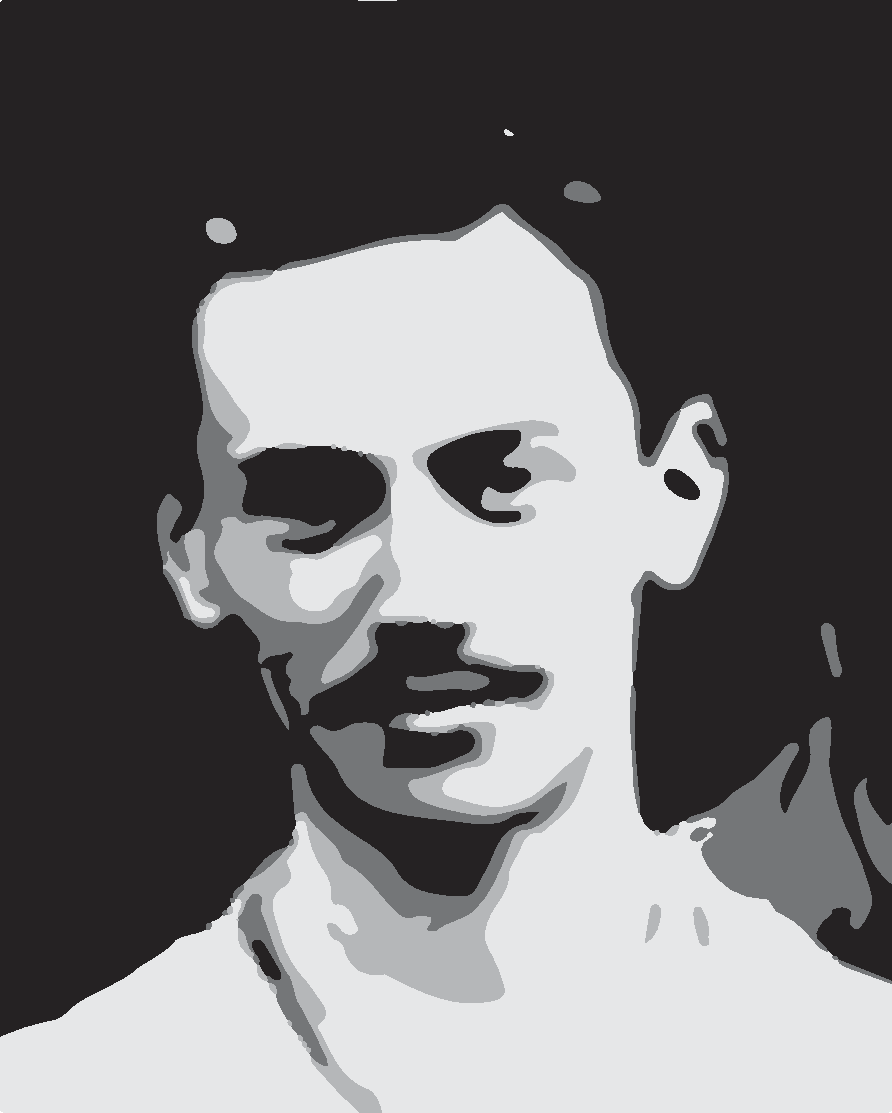
\includegraphics[height=.35\textwidth]{./fotos/calcasdos/gateaux.pdf}\\[5pt]
{\small \bfseries René Gâteaux}
\end{bio}

Cabe señalar que la existencia de la derivada direccional de
$\varphi $ en $u_{0}$ en la dirección de $v$ para toda $v\in V$ no
basta para garantizar que $\mathcal{G}\varphi (u_{0})\in
\mathcal{L}(V,W)$ [Ejercicio~\ref{noGdif}]. Tampoco basta con que
$\varphi $ sea Gâteaux-diferenciable para que sea diferenciable,
como lo muestra el siguiente ejemplo.

\begin{example}
  La función $\varphi \colon \mathbb{R}^{2}\rightarrow \mathbb{R}$ dada
  por
  \begin{equation*}
    \varphi (x,y):=
      \begin{cases}
        \frac{x^{3}y}{x^{4}+y^{2}} & \text{si $(x,y)\neq (0,0)$,} \\ 
        0 & \text{si $(x,y)=(0,0)$.}
      \end{cases}
  \end{equation*}
  es Gâteaux-diferenciable en $\mathbb{R}^{2}$ pero no es
  diferenciable en $(0,0)$ \emph{[Ejercicio~\ref{siGnoF}]}.
\end{example}

Sin embargo, se tiene el siguiente resultado.

\begin{theorem}
  \label{C1derG}$\varphi \colon \Omega \rightarrow W$ es de clase
  $\mathcal{C}^{1}$ en $\Omega $ si y sólo si $\varphi $ es
  Gâteaux-diferenciable en $\Omega $ y su derivada de Gâteaux
  $\mathcal{G}\varphi \colon \Omega \rightarrow \mathcal{L}(V,W)$ es
  continua. En tal caso, $\varphi^{\prime }=\mathcal{G}\varphi $.
\end{theorem}

{\abovedisplayskip=7.5pt
\belowdisplayskip=7.5pt
\begin{proof}
  $\Rightarrow )$: \ Al inicio de esta sección demostramos que, si
  $\varphi $ es diferenciable en $u_{0}$, entonces $\varphi $ es
  Gâteaux-diferenciable en $u_{0}$ y $\mathcal{G}\varphi
  (u_{0})=\varphi^{\prime }(u_{0})$. En consecuencia, si $\varphi $
  es de clase $\mathcal{C}^{1}$ en $\Omega $, entonces
  $\mathcal{G}\varphi =\varphi^{\prime }$ es continua.

  $\Leftarrow )$: \ Supongamos ahora que $\varphi $ es
  Gâteaux-diferenciable en $\Omega $ y que $\mathcal{G}\varphi
  \colon \Omega \rightarrow \mathcal{L}(V,W)$ es continua. Sean $u_{0}\in
  \Omega $ y $\varepsilon >0$. Entonces existe $\delta >0$ tal que
  $u_{0}+v\in \Omega $ y
  \begin{equation}
    \left\Vert \mathcal{G}\varphi (u_{0}+v)-\mathcal{G}\varphi
      (u_{0})\right\Vert_{\mathcal{L}(V,W)}<\varepsilon \text{\qquad si \ }\left\Vert v\right\Vert_{V}<\delta .  \label{contG}
  \end{equation}
  Para cada $v\in V$ con $\left\Vert v\right\Vert_{V}<\delta $
  definimos $\sigma_{v}\colon [0,1]\rightarrow W$ como
  \begin{equation*}
    \sigma_{v}(t):=\varphi (u_{0}+tv)-\varphi (u_{0})-\mathcal{G}\varphi (u_{0})\left[ tv\right] .
  \end{equation*}
  Entonces $\sigma_{v}$ es diferenciable en $(0,1)$ y su derivada es
  \begin{align*}
    \sigma_{v}^{\prime }(t) &=\lim_{h\rightarrow 0}\frac{\sigma
     _{v}(t+h)-\sigma_{v}(t)}{h} \\
    &=\lim_{h\rightarrow 0}\frac{\varphi (u_{0}+tv+hv)-\varphi (u_{0}+tv)-\mathcal{G}\varphi (u_{0})\left[ hv\right] }{h} \\
    &=\lim_{h\rightarrow 0}\frac{\varphi (u_{0}+tv+hv)-\varphi (u_{0}+tv)}{h}-\mathcal{G}\varphi (u_{0})v \\
    &=\mathcal{G}\varphi (u_{0}+tv)v-\mathcal{G}\varphi (u_{0})v.
  \end{align*}
  Se sigue de (\ref{contG}) que
  \begin{align*}
    \left\Vert \sigma_{v}^{\prime }(t)\right\Vert_{W} &\leq \left\Vert 
      \mathcal{G}\varphi (u_{0}+tv)-\mathcal{G}\varphi (u_{0})\right\Vert_{\mathcal{L}(V,W)}\left\Vert v\right\Vert_{V} \\
    &\leq\varepsilon \left\Vert v\right\Vert_{V}\text{\qquad }\forall t\in (0,1).
  \end{align*}
  Usando el teorema del valor medio (ver Teorema~\ref{tvm}) concluimos
  que
  \begin{align*}
    \left\Vert \varphi (u_{0}+v)-\varphi (u_{0})-\mathcal{G}\varphi
      (u_{0})v\right\Vert_{W} &=\left\Vert \sigma_{v}(1)-\sigma
     _{v}(0)\right\Vert_{W} \\
    &\leq \varepsilon \left\Vert v\right\Vert_{V}\text{\qquad si \ }\left\Vert
      v\right\Vert_{V}<\delta .
  \end{align*}
  Esto prueba que $\varphi $ es diferenciable en $u_{0}$ y que
  $\varphi^{\prime }(u_{0})=\mathcal{G}\varphi (u_{0})$. Como
  $\mathcal{G}\varphi $ es continua, $\varphi $ es de clase
  $\mathcal{C}^{1}$ en $\Omega $.
\end{proof}

El teorema anterior proporciona un criterio muy útil para
verificar la diferenciabilidad de una función y calcular su
derivada. Veamos un ejemplo.

\begin{example}
  Sea $f\colon \mathbb{R}\rightarrow \mathbb{R}$ una función de clase
  $\mathcal{C}^{1}$. La función $\varphi
  \colon \mathcal{C}^{0}[a,b]\rightarrow \mathbb{R}$ dada por
  \begin{equation*}
    \varphi (u):=\int_{a}^{b}f(u(t))dt
  \end{equation*}
  es de clase $\mathcal{C}^{1}$ en $\mathcal{C}^{0}[a,b]$\ y su
  derivada es
  \begin{equation*}
    \varphi^{\prime }(u)v:=\int_{a}^{b}f^{\prime }(u(t))v(t)dt.
  \end{equation*}
\end{example}}%

{\abovedisplayskip=7.5pt 
\belowdisplayskip=7.5pt 
\begin{proof}
  Probaremos primero que $\varphi $ es Gâteaux-diferenciable. Sean
  $u,v\in \mathcal{C}^{0}[a,b]$, $v\neq 0$, y $\varepsilon >0$.
  Denotemos por
  \begin{equation*}
    M:=\left\Vert u\right\Vert_{\infty }+\left\Vert v\right\Vert_{\infty }\text{\qquad y\qquad }\tilde{\varepsilon}:=\frac{\varepsilon }{(b-a)\left\Vert v\right\Vert_{\infty }}.
  \end{equation*}
  Como $f^{\prime }$ es uniformemente continua en $[-M,M]$ existe
  $\delta >0$ tal que
  \begin{equation*}
    \left\vert f^{\prime }(x)-f^{\prime }(y)\right\vert <\tilde{\varepsilon}\text{\qquad }\forall x,y\in [-M,M]\text{ con }\left\vert
      x-y\right\vert <\delta .
  \end{equation*}
  Del Corolario~\ref{cortvm} y la desigualdad anterior se sigue que,
  si $x,\,x+hz\in [-M,M]$ y $\left\vert hz\right\vert <\delta $, entonces % $s\in [0,1]$, entonces
  \begin{equation}
    \left\vert f(x+hz)-f(x)-f^{\prime }(x)hz)\right\vert \leq \sup_{s\in [0,1]}\left\vert f^{\prime }(x+shz)-f^{\prime }(x)\right\vert \left\vert
      hz\right\vert \leq\tilde{\varepsilon}\left\vert hz\right\vert .  \label{ejGat}
  \end{equation}
  Observa que
  \begin{equation*}
    \left\vert u(t)+hv(t)\right\vert \leq \left\Vert u\right\Vert_{\infty
    }+\left\Vert v\right\Vert_{\infty }=M\text{\qquad }\forall t\in [a,b],\text{ }h\in [0,1].
  \end{equation*}
  Por tanto, podemos aplicar la desigualdad (\ref{ejGat}) a $x:=u(t)$,
  $z:=v(t) $ y $0<\left\vert h\right\vert <\min \left\{1,\frac{\delta
  }{\left\Vert v\right\Vert_{\infty }}\right\}$ para obtener
  \begin{equation*}
    \left\vert \frac{f(u(t)+hv(t))-f(u(t))}{h}-f^{\prime }(u(t))v(t)\right\vert \leq\tilde{\varepsilon}\left\vert v(t)\right\vert \leq \frac{\varepsilon }{b-a}\text{\hspace{0.3in}}\forall t\in [a,b].
  \end{equation*}
  En consecuencia, si $0<\left\vert h\right\vert <\min
  \left\{1,\frac{\delta }{\left\Vert v\right\Vert_{\infty }}\right\}$, entonces
  \begin{multline*}
    \left\vert \frac{\varphi (u+hv)-\varphi (u)}{h}-\int_{a}^{b}f^{\prime
      }(u(t))v(t)dt\right\vert \\
    \leq \int_{a}^{b}\left\vert \frac{f(u(t)+hv(t))-f(u(t))}{h}-f^{\prime
      }(u(t))v(t)\right\vert dt\leq\varepsilon .
  \end{multline*}
  Esto prueba que
  \begin{equation*}
    \int_{a}^{b}f^{\prime }(u(t))v(t)dt=\lim_{h\rightarrow 0}\frac{\varphi
      (u+hv)-\varphi (u)}{h}=:\mathcal{G}\varphi (u)v.
  \end{equation*}

  La función $\mathcal{G}\varphi
  (u)\colon \mathcal{C}^{0}[a,b]\rightarrow \mathbb{R}$ es claramente lineal
  y, como
  \begin{equation*}
    \left\vert \mathcal{G}\varphi (u)v\right\vert \leq \biggl(
      \int_{a}^{b}\left\vert f^{\prime }(u(t))\right\vert dt\biggr) \left\Vert
      v\right\Vert_{\infty }\text{\qquad }\forall v\in \mathcal{C}^{0}[a,b],
  \end{equation*}
  la Proposición~\ref{lin+cont}\ asegura que $\mathcal{G}\varphi
  (u)$ es continua. Por tanto, $\varphi $ es Gâteaux-diferenciable
  en $u$ para todo $u\in \mathcal{C}^{0}[a,b]$.

  Probaremos ahora que $\mathcal{G}\varphi
  \colon \mathcal{C}^{0}[a,b]\rightarrow
  \mathcal{L}(\mathcal{C}^{0}[a,b],\mathbb{R})$ es continua. Sean
  $u_{0}\in \mathcal{C}^{0}[a,b]$ y $\varepsilon >0$. Denotemos por
  $M_{0}:=\left\Vert u_{0}\right\Vert_{\infty }+1$. Como $f^{\prime
  }$ es uniformemente continua en $[-M_{0},M_{0}]$, existe $\delta \in
  (0,1)$ tal que
  \begin{equation*}
    \left\vert f^{\prime }(x)-f^{\prime }(y)\right\vert <\frac{\varepsilon }{(b-a)}\text{\qquad }\forall x,y\in [-M_{0},M_{0}]\text{ con }\left\vert x-y\right\vert <\delta .
  \end{equation*}
  Observa que, si $\left\Vert u-u_{0}\right\Vert_{\infty }<\delta $,
  entonces
  \begin{equation*}
    \left\vert u(t)\right\vert \leq \left\Vert u\right\Vert_{\infty }\leq
    \left\Vert u_{0}\right\Vert_{\infty }+\left\Vert u-u_{0}\right\Vert
   _{\infty }\leq \left\Vert u_{0}\right\Vert_{\infty }+\delta <M_{0}\text{\qquad }\forall t\in [a,b].
  \end{equation*}
  Por tanto, para todo $v\in\mathcal{C}^0[a,b]$,
  \begin{equation*}
    \left\vert \mathcal{G}\varphi (u)v-\mathcal{G}\varphi (u_{0})v\right\vert
    \leq \int_{a}^{b}\left\vert f^{\prime }(u(t))-f^{\prime
      }(u_{0}(t))\right\vert \left\vert v(t)\right\vert dt<\varepsilon \left\Vert
      v\right\Vert_{\infty }.
  \end{equation*}
  En consecuencia,
  \begin{equation*}
    \left\Vert \mathcal{G}\varphi (u)-\mathcal{G}\varphi
      (u_{0})\right\Vert_{\mathcal{L}(\mathcal{C}^{0}[a,b],\mathbb{R})}=\sup_{\substack{
        v\in \mathcal{C}^{0}[a,b]  \\ v\neq 0}}\frac{\left\vert
        \mathcal{G}\varphi (u)v-\mathcal{G}\varphi (u_{0})v\right\vert
    }{\left\Vert v\right\Vert_{\infty }}\leq\varepsilon 
  \end{equation*}
  si $\left\Vert u-u_{0}\right\Vert_{\infty }<\delta$.  Esto prueba
  que
  $\mathcal{G}\varphi \colon \mathcal{C}^{0}[a,b]\rightarrow
  \mathcal{L}(\mathcal{C}^{0}[a,b],\mathbb{R})$ es continua.

  Del Teorema~\ref{C1derG}\ se sigue que $\varphi $ es de clase
  $\mathcal{C}^{1}$\ y que $\varphi^{\prime }=\mathcal{G}\varphi $.
\end{proof}

\section{Derivadas parciales}

Sean $V_{1},\dots,V_{n},W$ espacios de Banach. El producto cartesiano
$V_{1}\times \cdots \times V_{n}$ con la norma
\begin{equation*}
  \left\Vert (v_{1},\dots,v_{n})\right\Vert_{V_{1}\times \cdots \times
    V_{n}}:=\max_{j=1,\dots,n}\left\Vert v_{j}\right\Vert_{V_{j}}
\end{equation*}
es un espacio de Banach (ver Ejercicio~\ref{prodcompl}). La
inclusión en el $j$-ésimo factor,
\begin{equation*}
  \iota_{j}\colon V_{j}\rightarrow V_{1}\times \cdots \times V_{n},\text{\qquad }\iota_{j}(v):=(0,\dots,0,\underset{j\text{-ésimo}}{\undercbrace{v}},0,\dots,0),
\end{equation*}}%
es una función lineal y una isometría. Si $\Omega $ es
abierto en $V_{1}\times \cdots \times V_{n}$ y $u\in \Omega $,
entonces
\begin{equation*}
  \Omega_{j,u}:=\left\{v\in V_{j}:u+\iota_{j}v\in \Omega \right\}
\end{equation*}
es un abierto de $V_{j}$ que contiene a $0$.

\begin{figure}[htb]
  \centering
  \begin{tikzpicture}[scale=.65]
  \draw[very thin,fill=gray!25] plot[smooth cycle, tension=.75]
  coordinates{(-1,-2) (1,-2) (1.7,1.3) (-1,2) (-1,0.5) (0,.3)};
  \draw[only marks, mark=*, mark size=1.4pt] plot 
  coordinates{(0,-1.1) (-2.7,-6)};
  \node[above] at (0.1,-1.1) {$u$};
  \node[below] at (.8,1) {$\Omega$};
  \draw[dashed] (-.7,-1.1)--(1.5,-1.1);
  \draw[very thick] (-3.4,-6)--(-1,-6);
  \draw[-latex'] (-3.8,-6)--(3,-6);
  \draw[-latex'] (-2.7,-6.5)--(-2.7,-.5);
  \node[below] at (-3,-6) {{\footnotesize $0$}};
  \node[below] at (-1.7,-6) {$\Omega_{j,u}$};
  \node[below] at (7,1) {$W$};
  \draw[-latex'](2,.7) .. controls (3.2,1) and (5.3,1) .. 
  node[above] {$\varphi$} (6.6,.7);
  \draw[-latex'] (-2.6,-5.8) -- 
  node[left,label={[shift={(-0.26,-0.25)}]$u+\iota_j$}] {} (0,-1.2);
  \draw[-latex'] (-1.9,-5.8) -- % .. controls (2,-5) and (4,-3) .. 
  node[inner sep=10pt,right] {$\varphi_{j,u}$} (6.7,.3);
  \draw (-3.4,-6.1)--(-3.4,-5.9);
  \draw (-1,-6.1)--(-1,-5.9);
\end{tikzpicture}

  % \caption{}\label{fig:9.3}
\end{figure}

En lo que resta de esta sección supondremos que $\Omega $ es
abierto en $V_{1}\times \cdots \times V_{n}$.

\begin{definition}
  Una función $\varphi \colon \Omega \rightarrow W$ es
  \textbf{parcialmente diferenciable respecto a la
  }$j$\textbf{-ésima variable en el punto} $u$\textbf{\ de
  }$\Omega $\index{función!parcialmente diferenciable} si la
  función
  \begin{equation*}
    \varphi_{j,u}\colon \Omega_{j,u}\rightarrow W,\text{\qquad }\varphi_{j,u}(v):=\varphi (u+\iota_{j}v),
  \end{equation*}
  es diferenciable en $0$. La\textbf{\ derivada parcial de }$\varphi
  $\textbf{\ respecto a la }$j$\textbf{-ésima variable}
  \textbf{en} $u$ \index{derivada!parcial}se define como
  \begin{equation*}
    \partial_{j}\varphi (u):=\varphi_{j,u}^{\prime }(0)\in \mathcal{L}(V_{j},W).
  \end{equation*}
  La función $\varphi $ es \textbf{parcialmente diferenciable
    respecto a la }$j$\textbf{-ésima variable en} $\Omega $ si lo
  es en todo punto $u\in \Omega $, y \textbf{la derivada parcial de
  }$\varphi $\textbf{\ respecto a la }$j$\textbf{-ésima variable}
  en\textbf{\ }$\Omega $ es la función
  \begin{equation*}
    \partial_{j}\varphi \colon \Omega \rightarrow \mathcal{L}(V_{j},W),\text{\qquad }u\mapsto \partial_{j}\varphi (u).
  \end{equation*}
\end{definition}

Si $\varphi \colon \Omega \rightarrow W$ es diferenciable en $u$ entonces,
por la regla de la cadena, $\varphi $ es parcialmente diferenciable
respecto a la $j $-ésima variable en $u$ y
\begin{equation*}
  \partial_{j}\varphi (u)=\varphi^{\prime }(u)\circ \iota_{j},\text{\qquad }j=1,\dots,n.
\end{equation*}
Es decir, $\partial_{j}\varphi (u)$ es la restricción de $\varphi
^{\prime }(u)$\ al factor $V_{j}$. Nota que $v=\sum_{j=1}^{n}\iota
_{j}v_{j}$ si $v=(v_{1},\dots,v_{n})$. En consecuencia,
\begin{equation}
  \varphi^{\prime }(u)v=\sum_{j=1}^{n}\partial_{j}\varphi (u)v_{j}.\label{formparc}
\end{equation}

Los siguientes ejemplos relacionan estos conceptos con conceptos bien
conocidos de cálculo.

\begin{example}
  Si $\Omega $ es abierto en $\mathbb{R}^{n}=\mathbb{R}\times \cdots
  \times \mathbb{R}$ y $\varphi \colon \Omega \rightarrow \mathbb{R}$ es
  diferenciable en $x $, entonces $\partial_{j}\varphi (x)\in
  \mathcal{L}(\mathbb{R},\mathbb{R})\cong \mathbb{R}$. Como en la
  sección \emph{\ref{varreal}}, identificamos a la función
  lineal $\partial_{j}\varphi (x)$ con su valor en $1$. Ésta es
  la \textbf{derivada parcial de} $\varphi $\textbf{\ respecto a
  }$x_{j}$\textbf{\ }a la que se suele denotar por
  \begin{equation*}
    \frac{\partial \varphi }{\partial x_{j}}(x)\in \mathbb{R}.
  \end{equation*}
  El \textbf{gradiente de }$\varphi $\textbf{\ en }$x$
  \index{gradiente}es el vector
  \begin{equation*}
    \nabla \varphi (x):=\left( 
      \frac{\partial \varphi }{\partial x_{1}}(x),\dots,\frac{\partial \varphi }{\partial x_{n}}(x)\right) \in \mathbb{R}^{n}.
  \end{equation*}
  La fórmula \emph{(\ref{formparc})} se escribe entonces como
  \begin{equation*}
    \varphi^{\prime }(x)y=\sum_{j=1}^{n}\frac{\partial \varphi }{\partial x_{j}}(x)y_{j}=\nabla \varphi (x)\cdot y,
  \end{equation*}
  donde $\nabla \varphi (x)\cdot y$ denota al producto escalar usual
  de los vectores $\nabla \varphi (x)$ y $y$ en $\mathbb{R}^{n}$.
\end{example}

\begin{example}
  Si $\Omega $ es abierto en $\mathbb{R}^{n}$ y $\varphi =(\varphi
 _{1},\dots,\varphi_{m})\colon \Omega \rightarrow \mathbb{R}^{m}$ es
  diferenciable en $x$, entonces la $j$-ésima componente $\varphi
 _{j}$ de $\varphi $ es la composición $\varphi_{j}:=\pi
 _{j}\circ \varphi $ con la $j$-ésima proyección
  \begin{equation*}
    \pi_{j}\colon \mathbb{R}^{m}\rightarrow \mathbb{R},\text{\qquad }\pi
   _{j}(z_{1},\dots,z_{m}):=z_{j}.
  \end{equation*}
  Como $\pi_{j}$ es lineal, aplicando la regla de la cadena se tiene
  que
  \begin{equation*}
    \varphi_{j}^{\prime }(x)=\pi_{j}\circ \varphi^{\prime }(x),
  \end{equation*}
  es decir, $\varphi_{j}^{\prime }(x)$ es la $j$-ésima componente
  de $\varphi^{\prime }(x)$. Por tanto,
  \begin{align*}
    \varphi^{\prime }(x)y &=(\varphi_{1}^{\prime }(x)y,\dots,\varphi
   _{m}^{\prime }(x)y) \\
    &=(\nabla \varphi_{1}(x)\cdot y,\dots,\nabla \varphi_{m}(x)\cdot y),
  \end{align*}
  es decir, $\varphi^{\prime }(x)$ es la función lineal dada por
  la matriz
  \begin{equation*}
    \varphi^{\prime }(x)= 
      \begin{pmatrix}
        \frac{\partial \varphi_{1}}{\partial x_{1}}(x) & \cdots & \frac{\partial
          \varphi_{1}}{\partial x_{n}}(x) \\ 
        \vdots &  & \vdots \\ 
        \frac{\partial \varphi_{m}}{\partial x_{1}}(x) & \cdots & \frac{\partial
          \varphi_{m}}{\partial x_{n}}(x)
      \end{pmatrix}
  \end{equation*}
  que se llama la \textbf{matriz jacobiana\ d}e $\varphi $ \textbf{en}
  $x$.\index{matriz!jacobiana}
\end{example}

No es cierto, en general, que si $\varphi $ es parcialmente
diferenciable respecto a cada variable en $u$ entonces $\varphi $ es
diferenciable en $u$ [Ejercicio~\ref{siGnoF}]. Pero sí lo es si
se cumple además que $\partial_{j}\varphi $ es continua en
$\Omega $ para toda $j=1,\dots,n$.

\begin{theorem}
  Una función $\varphi \colon \Omega \rightarrow W$ es de clase
  $\mathcal{C}^{1}$ en $\Omega $ si y sólo si $\varphi $ es
  parcialmente diferenciable respecto a la $j$-ésima variable en
  $\Omega $ y
  \begin{equation*}
    \partial_{j}\varphi \colon \Omega \rightarrow \mathcal{L}(V_{j},W)
  \end{equation*}
  es continua en $\Omega $ para todo\ $j=1,\dots,n$.
\end{theorem}

\begin{proof}
  $\Rightarrow )$: \ Ya vimos que, si $\varphi \colon \Omega \rightarrow W$
  es diferenciable en $u$, entonces $\varphi $ es parcialmente
  diferenciable respecto a la $j$-ésima variable en $u$ y
  $\partial_{j}\varphi (u)=\varphi^{\prime }(u)\circ \iota_{j}$.
  Por tanto, $\partial_{j}\varphi $ es continua si $\varphi $ es de
  clase $\mathcal{C}^{1}$ en $\Omega $.

  $\Leftarrow )$: \ Supongamos ahora que $\varphi $ es parcialmente
  diferenciable respecto a la $j$-ésima variable en $\Omega $ y
  que $\partial_{j}\varphi $ es continua en $\Omega $ para todo\
  $j=1,\dots,n$.  Basta considerar el caso $n=2$, ya que el caso general
  se obtiene iterando éste.

  Sean $u=(u_{1},u_{2})\in \Omega $ y $\varepsilon >0$. Como $\varphi
  $ es diferenciable respecto a la primera variable en $u$ y $\partial
 _{2}\varphi $ es continua en $u$, existe $\delta >0$ tal que
  \begin{equation*}
    u+v\in \Omega 
    \text{\qquad si }v=(v_{1},v_{2})\in V_{1}\times V_{2}\text{ \ y \ }\left\Vert v\right\Vert_{V_{1}\times V_{2}}:=\max \left\{\left\Vert
      v_{1}\right\Vert_{V_{1}},\left\Vert v_{2}\right\Vert_{V_{2}}\right\}<\delta ,
  \end{equation*}
  \begin{align}
    \left\Vert \varphi (u+\iota_{1}v_{1})-\varphi (u)-\partial_{1}\varphi
      (u)v_{1}\right\Vert_{W} &\leq\frac{\varepsilon }{4}\left\Vert
      v_{1}\right\Vert_{V_{1}}\text{\qquad si }\left\Vert v_{1}\right\Vert
   _{V_{1}}<\delta ,  \label{dp1} \\
    \left\Vert \partial_{2}\varphi (u+v)-\partial_{2}\varphi (u)\right\Vert_{\mathcal{L}(V_{2},W)} &<\frac{\varepsilon }{4}\text{\qquad si }\left\Vert
      v\right\Vert_{V_{1}\times V_{2}}<\delta .  \notag
  \end{align}
  La segunda desigualdad implica que
  \begin{align}
    \left\Vert \partial_{2}\varphi (u+\iota_{1}v_{1})v_{2}-\partial
     _{2}\varphi (u)v_{2}\right\Vert_{W} &\leq \left\Vert \partial_{2}\varphi
      (u+\iota_{1}v_{1})-\partial_{2}\varphi (u)\right\Vert_{\mathcal{L}(V_{2},W)}\left\Vert v_{2}\right\Vert_{V_{2}}  \notag \\
    &\leq\frac{\varepsilon }{4}\left\Vert v_{2}\right\Vert_{V_{2}}\text{\qquad si 
    }\left\Vert v_{1}\right\Vert_{V_{1}}<\delta ,  \label{dp2}
  \end{align}
  y también que
  \begin{align*}
    &\left\Vert \partial_{2}\varphi (u+\iota_{1}v_{1}+t\iota
     _{2}v_{2})-\partial_{2}\varphi (u+\iota_{1}v_{1})\right\Vert_{\mathcal{L}(V_{2},W)} \\[4pt]
    &\quad{}\leq \left\Vert \partial_{2}\varphi (u+\iota_{1}v_{1}+t\iota
     _{2}v_{2})-\partial_{2}\varphi (u)\right\Vert_{\mathcal{L}(V_{2},W)}+\left\Vert \partial_{2}\varphi (u)-\partial_{2}\varphi (u+\iota
     _{1}v_{1})\right\Vert_{\mathcal{L}(V_{2},W)} \\[4pt]
    &\quad{}<\tfrac{\varepsilon }{2}\text{\qquad si }\left\Vert v\right\Vert
   _{V_{1}\times V_{2}}<\delta \text{ \ y \ }t\in [0,1].
  \end{align*}
  De esta última desigualdad y el Corolario~\ref{cortvm}\ se sigue
  que
  \begin{align}
    &\left\Vert \varphi (u+v)-\varphi (u+\iota_{1}v_{1})-\partial_{2}\varphi
      (u+\iota_{1}v_{1})v_{2}\right\Vert_{W}  \notag \\[4pt]
    &\quad{}\leq \sup_{t\in [0,1]}\left\Vert \partial_{2}\varphi (u+\iota
     _{1}v_{1}+t\iota_{2}v_{2})-\partial_{2}\varphi (u+\iota
     _{1}v_{1})\right\Vert_{\mathcal{L}(V_{2},W)}\left\Vert v_{2}\right\Vert
   _{V_{2}}  \notag \\[4pt]
    &\quad{}\leq\tfrac{\varepsilon }{2}\left\Vert v_{2}\right\Vert_{V_{2}}\text{\qquad si 
    }\left\Vert v\right\Vert_{V_{1}\times V_{2}}<\delta .  \label{dp3}
  \end{align}
  Finalmente, de las desigualdades (\ref{dp1}), (\ref{dp2}) y
  (\ref{dp3}) obtenemos
  \begin{align*}
    &\left\Vert \varphi (u+v)-\varphi (u)-\partial_{1}\varphi
      (u)v_{1}-\partial_{2}\varphi (u)v_{2}\right\Vert \\[4pt]
    &\quad{}\leq \left\Vert \varphi (u+v)-\varphi (u+\iota_{1}v_{1})-\partial
     _{2}\varphi (u+\iota_{1}v_{1})v_{2}\right\Vert\\[4pt]
    &\qquad{}+\left\Vert \partial
     _{2}\varphi (u+\iota_{1}v_{1})v_{2}-\partial_{2}\varphi (u)v_{2}\right\Vert
    +\left\Vert \varphi (u+\iota_{1}v_{1})-\varphi (u)-\partial_{1}\varphi
      (u)v_{1}\right\Vert \\[4pt]
    &\quad{}\leq \varepsilon \left\Vert v\right\Vert_{V_{1}\times V_{2}}\text{\qquad
      si }\left\Vert v\right\Vert_{V_{1}\times V_{2}}<\delta .
  \end{align*}
  Esto prueba que $\varphi $ es diferenciable en $u$ y que $\varphi
 ^{\prime }(u)v=\partial_{1}\varphi (u)v_{1}+\partial_{2}\varphi
  (u)v_{2}$. Por tanto, $\varphi $ es de clase $\mathcal{C}^{1}$ en
  $\Omega $.
\end{proof}

\section{Derivadas de orden superior}

Sean $V$ y $W$ espacios de Banach y $\Omega $ un subconjunto abierto
de $V$. Si $\varphi \colon \Omega \rightarrow W$ es diferenciable en $\Omega
$, su derivada es una función que toma valores en el espacio de
Banach $\mathcal{L}(V,W)$. Tiene pues sentido preguntarnos si $\varphi
^{\prime }\colon \Omega \rightarrow \mathcal{L}(V,W)$ es, a su vez,
diferenciable en $\Omega $. Si lo es, decimos que $\varphi $ es dos
veces diferenciable en $\Omega $. La derivada de $\varphi^{\prime }$
se llama la segunda derivada de $\varphi $ y se denota por
\begin{equation*}
  D^{2}\varphi \colon \Omega \rightarrow \mathcal{L}(V,\mathcal{L}(V,W)),
\end{equation*}
o simplemente por $\varphi^{\prime \prime }$. Veremos a
continuación que el espacio $\mathcal{L}(V,\mathcal{L}(V,W))$
tiene una representación sencilla: es el espacio de funciones
bilineales y continuas $V\times V\rightarrow W$.

Sean $V_{1},\dots,V_{k},W$ espacios de Banach.

\begin{definition}
  Una función $F\colon V_{1}\times \cdots \times V_{k}\rightarrow W$ es
  $k$\textbf{-multilineal} \index{función!multilineal}si es lineal
  en cada variable, es decir, si para cada $j\in \left\{1,\ldots ,k\right\}$ y
  $u_{i}\in V_{i}$, $i\neq j$, la función $V_{j}\rightarrow W$
  dada por
  \begin{equation*}
    v\longmapsto F[u_{1},\dots,u_{j-1},v,u_{j+1},\dots,u_{m}]
  \end{equation*}
  es lineal. Si $k=2$ se dice que $F$ es
  \textbf{bilineal}.\index{función!bilineal}
\end{definition}

Denotamos por\index{espacio!L (V1)@$\mathcal{L}(V_{1},\dots,V_{k};W)$}
\begin{equation*}
  \mathcal{L}(V_{1},\dots,V_{k};W):=\left\{F\colon V_{1}\times \cdots \times
  V_{k}\rightarrow W:F\text{ es }k\text{-multilineal y continua}\right\}.
\end{equation*}
Si $V_{1}=\cdots =V_{k}=V$ escribimos simplemente
\index{espacio!L subk VW@$\mathcal{L}_{k}(V,W)$}
\begin{equation*}
  \mathcal{L}_{k}(V,W):=\mathcal{L}(\undercbrace{V,\dots,V}_{\text{$k$ veces}};W).
\end{equation*}
Como en el caso $k=1$ se tiene el siguiente resultado.

\begin{proposition}
  Si $F\colon V_{1}\times \cdots \times V_{k}\rightarrow W$ es
  $k$-multilineal, entonces $F$ es continua si y sólo si existe
  $c\in \mathbb{R}$ tal que
  \begin{equation}
    \left\Vert F[v]\right\Vert_{W}\leq c\left\Vert v_{1}\right\Vert
   _{V_{1}}\cdots \left\Vert v_{k}\right\Vert_{V_{k}}\text{\qquad }\forall
    v=(v_{1},\dots,v_{k})\in V_{1}\times \cdots \times V_{k}.  \label{mul}
  \end{equation}
\end{proposition}

\begin{proof}
  $\Rightarrow )$: \ Si $F$ es continua, existe $\delta >0$ tal que
  \begin{equation*}
    \left\Vert F[v]\right\Vert_{W}<1\text{\qquad si }\left\Vert v\right\Vert
   _{V_{1}\times \cdots \times V_{k}}:=\max_{j=1,\dots,k}\left\Vert
      v_{j}\right\Vert_{V_{j}}<\delta .
  \end{equation*}
  Por tanto, para todo $v=(v_{1},\dots,v_{k})\in V_{1}\times \cdots
  \times V_{k},$ tal que $v_i\neq 0$ para todo $i=1,\ldots,k$,
  \begin{equation*}
    \frac{\delta^{k}}{2^{k}\left\Vert v_{1}\right\Vert_{V_{1}}\cdots
      \left\Vert v_{k}\right\Vert_{V_{k}}}\left\Vert F[v]\right\Vert
   _{W}=\left\Vert F\left[ \frac{\delta }{2}\left( \frac{v_{1}}{\left\Vert
              v_{1}\right\Vert_{V_{1}}},\ldots ,\frac{v_{k}}{\left\Vert v_{k}\right\Vert
           _{V_{k}}}\right) \right] \right\Vert_{W}<1.
  \end{equation*}
  En consecuencia,
  \begin{equation*}
    \left\Vert F[v]\right\Vert_{W}\leq \frac{2^{k}}{\delta^{k}}\left\Vert
      v_{1}\right\Vert_{V_{1}}\cdots \left\Vert v_{k}\right\Vert_{V_{k}}\text{\qquad }\forall v=(v_{1},\dots,v_{k})\in V_{1}\times \cdots \times V_{k}.
  \end{equation*}

  $\Leftarrow )$: \ Supongamos ahora que se cumple (\ref{mul}). Sean
  $u,v\in V_{1}\times \cdots \times V_{k}$ y $R:=\left\Vert
    u\right\Vert_{V_{1}\times \cdots \times V_{k}}+1$. 
Como $F$ es
  $k$-multilineal,

  \begin{align*}
    F[v]-F[u] &=F[v_{1}-u_{1},v_{2},\dots,v_{k}] \\[5pt]
    &\qquad{}+\sum_{i=2}^{k-1}F[u_{1},\dots,u_{i-1},v_{i}-u_{i},v_{i+1},\dots,v_{k}]\\[5pt]
    &\qquad{}+F[u_{1},\dots,u_{k-1},v_{k}-u_{k}].
  \end{align*}
  Aplicando la desigualdad del triángulo y la desigualdad
  (\ref{mul}) concluimos que
{\small
  \begin{align*}
    \left\Vert F[v]-F[u]\right\Vert_{W} &\leq{} c\left\Vert
      v_{1}-u_{1}\right\Vert_{V_{1}}\left\Vert v_{2}\right\Vert_{V_{2}}\cdots
    \left\Vert v_{k}\right\Vert_{V_{k}} \\[3pt]
    &\qquad{}+c\sum_{i=2}^{k-1}\left\Vert u_{1}\right\Vert_{V_{1}}\cdots
    \left\Vert u_{i-1}\right\Vert_{V_{i-1}}\left\Vert v_{i}-u_{i}\right\Vert
   _{V_{i}}\left\Vert v_{i+1}\right\Vert_{V_{i+1}}\cdots \left\Vert
      v_{k}\right\Vert_{V_{k}} \\[3pt]
    &\qquad{}+c\left\Vert u_{1}\right\Vert_{V_{1}}\cdots \left\Vert u_{k-1}\right\Vert
   _{V_{k-1}}\left\Vert v_{k}-u_{k}\right\Vert_{V_{k}} \\[5pt]
    &\leq cR^{k-1}\sum_{i=1}^{k}\left\Vert v_{i}-u_{i}\right\Vert
   _{V_{i}}\text{\qquad si }\left\Vert v-u\right\Vert_{V_{1}\times \cdots
      \times V_{k}}<1.
  \end{align*}}
  De esta desigualdad se sigue inmediatamente que $F$ es continua en
  $u$.
\end{proof}

Para $F\in \mathcal{L}(V_{1},\dots,V_{k};W)$ definimos
\begin{equation}
  \left\Vert F\right\Vert_{\mathcal{L}(V_{1},\dots,V_{k};W)}:=\sup_{\substack{ v_{j}\in V_{j}\smallsetminus \left\{0\right\}  \\ j=1,\ldots ,k}}\frac{\left\Vert
      F[v_{1},\dots,v_{k}]\right\Vert_{W}}{\left\Vert v_{1}\right\Vert
   _{V_{1}}\cdots \left\Vert v_{k}\right\Vert_{V_{k}}}.  \label{normul}
\end{equation}
Esta es una norma en $\mathcal{L}(V_{1},\dots,V_{k};W)$, que coincide
con la definida en (\ref{defnorma}) cuando $k=1$.

Asociando a cada $F\in \mathcal{L}(V_{1},\dots,V_{k};W)$ la función
$\hat{F}\in \mathcal{L}(V_{1},\mathcal{L}(V_{2},\dots ,V_{k};W))$
dada por
\begin{equation*}
  (\hat{F}v_{1})[v_{2},\ldots ,v_{k}]:=F[v_{1},v_{2},\ldots ,v_{k}],\text{\qquad }v_{j}\in V_{j},
\end{equation*}
obtenemos un isomorfismo de espacios vectoriales
\begin{equation}
  \mathcal{L}(V_{1},\dots,V_{k};W)\cong \mathcal{L}(V_{1},\mathcal{L}(V_{2},\dots ,V_{k};W))  \label{bil}
\end{equation}
que es además una isometría, es decir,
\begin{equation*}
  \bigl\Vert F\bigr\Vert_{\mathcal{L}(V_{1},\dots,V_{k};W)}=\bigl\Vert \hat{F}\bigr\Vert_{\mathcal{L}(V_{1},\mathcal{L}(V_{2},\dots ,V_{k};W))}
\end{equation*}
[Ejercicio~\ref{multi}]. Iterando estos isomorfismos obtenemos 
\begin{equation*}
  \mathcal{L}(V_{1},\dots,V_{k};W)\cong \mathcal{L}(V_{1},\mathcal{L}(V_{2},\cdots ,\mathcal{L}(V_{k-1},\mathcal{L}(V_{k},W))\cdots )).
\end{equation*}
En consecuencia, $\mathcal{L}(V_{1},\dots,V_{k};W)$\ es un espacio de
Banach (ver Proposición~\ref{lin+contBanach}).

Podemos definir ahora las derivadas de orden superior como sigue.

\begin{definition}
  Sea $k\in \mathbb{N}$, $k\geq 2$. Una función $\varphi \colon \Omega
  \rightarrow W$ es $k$\textbf{-veces diferenciable en} $\Omega $ si
  $\varphi $ es $(k-1)$-veces diferenciable en $\Omega $ y su derivada
  de orden $k-1$ es diferenciable en $\Omega $. La derivada de
  $D^{k-1}\varphi \colon \Omega \rightarrow \mathcal{L}_{k-1}(V,W)$ se llama
  la \textbf{derivada de orden }$k $\textbf{\ de }$\varphi $
  \index{derivada!de orden k@de orden $k$}y se denota
  \begin{equation*}
    D^{k}\varphi \colon \Omega \rightarrow \mathcal{L}(V,\mathcal{L}_{k-1}(V,W))\cong 
    \mathcal{L}_{k}(V,W).
  \end{equation*}
  Si $D^{k}\varphi $ es continua en $\Omega $ decimos que $\varphi
  $\textbf{\ es de clase }$\mathcal{C}^{k}$\textbf{\ en }$\Omega $.
  \index{función!de clase ck@de clase $\mathcal{C}^{k}$}

  Si $D^{j}\varphi $ admite una extensión continua a la cerradura
  $\overline{\Omega }$ de $\Omega $ para cada $j=0,1,\ldots ,k$, donde
  $D^{0}\varphi :=\varphi $, decimos que $\varphi $\textbf{\ es de
    clase }$\mathcal{C}^{k}$\textbf{\ en} $\overline{\Omega }$.

  Finalmente, si $\varphi $ es de clase $\mathcal{C}^{k}$\textbf{\ }en
  $\Omega $ (resp. en $\overline{\Omega }$) para todo $k\in
  \mathbb{N}$, decimos que $\varphi $\textbf{\ es de clase
  }$\mathcal{C}^{\infty }$\textbf{\ en }$\Omega $ (resp. en
  $\overline{\Omega }$).
\end{definition}

Veamos un ejemplo.

\begin{example}
  La función $\varphi \colon \ell_{2}\rightarrow \mathbb{R}$ dada por
  $\varphi (\overline{x}):=\left\Vert \overline{x}\right\Vert_{\ell
   _{2}}^{2}$ es de clase $\mathcal{C}^{\infty }$ en $\ell_{2}$,
  \begin{equation*}
    D^{2}\varphi (\overline{x})[\overline{y},\overline{z}]=2\sum_{k=1}^{\infty }y_{k}z_{k}\text{\qquad }\forall \overline{x},\overline{y},\overline{z}\in \ell_{2},
  \end{equation*}
  y $D^{k}\varphi (\overline{x})=0\in \mathcal{L}_{k}(\ell
 _{2},\mathbb{R})$ para todo $\overline{x}\in \ell_{2}$, $k\geq 3$.
\end{example}

\begin{proof}
  Sabemos que $\varphi $ es diferenciable, que su derivada $\varphi
 ^{\prime }\colon \ell_{2}\rightarrow \mathcal{L}(\ell_{2},\mathbb{R})$
  está dada por
  \begin{equation*}
    \varphi^{\prime }(\overline{x})\overline{z}=2\sum_{k=1}^{\infty
    }x_{k}z_{k}\text{\qquad }\forall \overline{x}=(x_{k}),\text{ }\overline{z}=(z_{k})\in \ell_{2}
  \end{equation*}
  (ver Ejemplo~\ref{ejder3}) y que $\varphi^{\prime }$ es continua
  (ver Ejemplo~\ref{ejder4}). Observa además que $\varphi^{\prime
  }$ es lineal, es decir,
  \begin{equation*}
    \varphi^{\prime }(\alpha \overline{x}+\beta \overline{y})=\alpha \varphi
   ^{\prime }(\overline{x})+\beta \varphi^{\prime }(\overline{y})\text{\qquad }\forall \overline{x},\overline{y}\in \ell_{2},\text{ }\forall \alpha ,\beta
    \in \mathbb{R}.
  \end{equation*}
  El Ejemplo~\ref{ejder2}\ asegura entonces que $D^{2}\varphi
  (\overline{x})=\varphi^{\prime }$ para todo $\overline{x}\in \ell
 _{2}$, y usando el isomorfismo (\ref{bil}) obtenemos
{\abovedisplayskip=9pt 
\belowdisplayskip=9pt 
  \begin{equation*}
    D^{2}\varphi (\overline{x})[\overline{y},\overline{z}]=\varphi^{\prime }[\overline{y},\overline{z}]=\varphi^{\prime }(\overline{y})\overline{z}=2\sum_{k=1}^{\infty }y_{k}z_{k}\text{\qquad }\forall \overline{x},\overline{y},\overline{z}\in \ell_{2}.
  \end{equation*}
  Más aún, como
  $D^{2}\varphi \colon \ell_{2}\rightarrow
  \mathcal{L}_{2}(\ell_{2},\mathbb{R})$
  es constante, el Ejemplo~\ref{ejder1} asegura que
  $D^{k}\varphi (\overline{x})=0\in
  \mathcal{L}_{k}(\ell_{2},\mathbb{R})$
  para todo $\overline{x}\in \ell_{2}$, $k\geq 3$.}
\end{proof}

Como ocurre en espacios euclidianos, la derivada de orden $k$ en cada
punto es simétrica.

{\abovedisplayskip=9pt 
\belowdisplayskip=9pt 
\begin{proposition}
  \label{sim}Si $\varphi \colon \Omega \rightarrow W$ es $k$-veces
  diferenciable en $\Omega $ entonces, para cada $u\in \Omega $, la
  $k$-ésima derivada de $\varphi $ en $u$ es simétrica, es
  decir,
  \begin{equation*}
    D^{k}\varphi (u)[v_{1},\ldots ,v_{k}]=D^{k}\varphi (u)[v_{\tau (1)},\ldots
    ,v_{\tau (k)}]
  \end{equation*}
  para cualesquiera $v_{1},\ldots ,v_{k}\in V$ y cualquier
  permutación $\tau \colon \left\{1,\ldots ,k\right\}\rightarrow \left\{1,\ldots ,k\right\}$.
\end{proposition}

\begin{proof}
  Consideramos dos casos.

  \textsc{Caso 1: }$k=2$.

  Sean $u\in \Omega $ y $\varepsilon >0$. Como $\varphi $ es dos veces
  diferenciable en $u$ existe $\delta >0$ tal que $u+v\in \Omega $ y
  \begin{equation}
    \left\Vert \varphi^{\prime }(u+v)-\varphi^{\prime }(u)-D^{2}\varphi
      (u)v\right\Vert_{\mathcal{L}(V,W)}\leq\varepsilon \left\Vert v\right\Vert_{V}\text{\qquad si }\left\Vert v\right\Vert_{V}<2\delta .  \label{2dif}
  \end{equation}
  Sean $v,w\in V$ tales que $\max \left\{\left\Vert v\right\Vert
 _{V},\left\Vert w\right\Vert_{V}\right\}<\delta $. Definimos $\sigma
  \colon [0,1]\rightarrow W$ como
  \begin{equation*}
    \sigma (t):=\varphi (u+tv+w)-\varphi (u+tv).
  \end{equation*}
  Entonces
  \begin{align*}
    \sigma^{\prime }(t)-D^{2}\varphi (u)[w,v] &=\left[ \varphi^{\prime
      }(u+tv+w)v-\varphi^{\prime }(u)v-D^{2}\varphi (u)[tv+w,v]\right] \\
    &\qquad{}-\left[ \varphi^{\prime }(u+tv)v-\varphi^{\prime }(u)v-D^{2}\varphi
      (u)[tv,v]\right]
  \end{align*}
  y aplicando (\ref{2dif}) obtenemos
  \begin{align*}
    &\left\Vert \sigma^{\prime }(t)-D^{2}\varphi
    (u)[w,v]\right\Vert_{W}\\ 
    &\qquad{}\leq
    \left\Vert \varphi^{\prime }(u+tv+w)-\varphi^{\prime }(u)-D^{2}\varphi
      (u)[tv+w]\right\Vert_{\mathcal{L}(V,W)}\left\Vert v\right\Vert_{V} \\
    &\qquad\qquad{}+\left\Vert \varphi^{\prime }(u+tv)-\varphi^{\prime }(u)-D^{2}\varphi
      (u)(tv)\right\Vert_{\mathcal{L}(V,W)}\left\Vert v\right\Vert_{V} \\
    &\qquad{}<2\varepsilon \left( \left\Vert v\right\Vert_{V}+\left\Vert w\right\Vert
     _{V}\right) \left\Vert v\right\Vert_{V}\text{\qquad }\forall t\in [0,1].
  \end{align*}
  El Corolario~\ref{cortvm}\ y la desigualdad anterior implican que
  \begin{align*}
    &\left\Vert \sigma (1)-\sigma (0)-D^{2}\varphi
      (u)[w,v]\right\Vert_{W}\\ 
      &\qquad{}\leq\left\Vert \sigma (1)-\sigma (0)-\sigma^{\prime }(0)\right\Vert
   _{W}
    +\left\Vert \sigma^{\prime }(0)-D^{2}\varphi (u)[w,v]\right\Vert_{W} \\
    &\qquad\leq \sup_{t\in [0,1]}\left\Vert \sigma^{\prime }(t)-\sigma
     ^{\prime }(0)\right\Vert_{W}
    +\left\Vert \sigma^{\prime }(0)-D^{2}\varphi
      (u)[w,v]\right\Vert_{W} \\
    &\qquad{}\leq 3\sup_{t\in [0,1]}\left\Vert \sigma^{\prime }(t)-D^{2}\varphi
      (u)[w,v]\right\Vert_{W} \\
    &\qquad{}\leq 6\varepsilon \left( \left\Vert v\right\Vert_{V}+\left\Vert
        w\right\Vert_{V}\right) \left\Vert v\right\Vert_{V}.
  \end{align*}
  Observa que $\sigma (1)-\sigma (0)=\varphi (u+v+w)-\varphi
  (u+v)-\varphi (u+w)+\varphi (u)$ es simétrica en $v$ y $w$, por
  lo que intercambiando los papeles de $v$ y $w$ en la desigualdad
  anterior obtenemos
  \begin{equation*}
    \left\Vert \sigma (1)-\sigma (0)-D^{2}\varphi (u)[v,w]\right\Vert_{W}\leq
    6\varepsilon \left( \left\Vert v\right\Vert_{V}+\left\Vert w\right\Vert
     _{V}\right) \left\Vert w\right\Vert_{V}.
  \end{equation*}
  En consecuencia,
  \begin{equation*}
    \left\Vert D^{2}\varphi (u)[v,w]-D^{2}\varphi (u)[w,v]\right\Vert_{W}\leq
    6\varepsilon \left( \left\Vert v\right\Vert_{V}+\left\Vert w\right\Vert
     _{V}\right)^{2}
  \end{equation*}
  si
  $\max \left\{\left\Vert v\right\Vert _{V},\left\Vert
      w\right\Vert_{V}\right\}<\delta$.

  Si $v,w\in V$ son arbitrarios, escogemos $\lambda \in (0,1]$ tal que
  $\max \left\{\left\Vert \lambda v\right\Vert_{V},\left\Vert \lambda
    w\right\Vert_{V}\right\}<\delta $. De la desigualdad anterior se sigue
  entonces que
  \begin{align*}
    \left\Vert D^{2}\varphi (u)[v,w]-D^{2}\varphi (u)[w,v]\right\Vert_{W} &=\frac{1}{\lambda^{2}}\left\Vert D^{2}\varphi (u)[\lambda v,\lambda
      w]-D^{2}\varphi (u)[\lambda w,\lambda v]\right\Vert_{W} \\
    &\leq \frac{1}{\lambda^{2}}6\varepsilon \left( \left\Vert \lambda
        v\right\Vert_{V}+\left\Vert \lambda w\right\Vert_{V}\right)^{2}\\
    &=6\varepsilon \left( \left\Vert v\right\Vert_{V}+\left\Vert
        w\right\Vert_{V}\right)^{2}.
  \end{align*}
  Como $\varepsilon >0$ es arbitraria, concluimos que $D^{2}\varphi
  (u)[v,w]=D^{2}\varphi (u)[w,v]$ para cualesquiera $v,w\in V$.

  \textsc{Caso 2: }$k>2$.

  El resultado se obtiene por inducción usando el caso $k=2$ y el
  isomorfismo (\ref{bil}).
\end{proof}}%

\begin{definition}
  \label{defCk}Si $V$ y $W$ son espacios de Banach, $\Omega $ es un
  subconjunto abierto de $V$ y $k\in \mathbb{N}\cup \left\{\infty \right\}$\
  definimos
\index{espacio!C alakOmega@$\mathcal{C}^{k}(\Omega ,W)$, $\mathcal{C}^{k}(\Omega )$}
\index{espacio!C alakOmegaO@ $\mathcal{C}^{k}(\overline{\Omega },W)$, $\mathcal{C}^{k}(\overline{\Omega })$}
  \begin{align*}
    \mathcal{C}^{k}(\Omega ,W) &:=\left\{\varphi \colon \Omega \rightarrow W:\varphi \text{
      es de clase }\mathcal{C}^{k}\text{ en }\Omega \right\}, \\
    \mathcal{C}^{k}(\overline{\Omega },W) &:=\left\{\varphi \colon \overline{\Omega }\rightarrow W:\varphi \text{ es de clase }\mathcal{C}^{k}\text{ en }\overline{\Omega }\right\}.
  \end{align*}
  Si $W=\mathbb{R}$ escribiremos simplemente
  \begin{align*}
    \mathcal{C}^{k}(\Omega ) &:=\mathcal{C}^{k}(\Omega ,\mathbb{R}), \\
    \mathcal{C}^{k}(\overline{\Omega }) &:=\mathcal{C}^{k}(\overline{\Omega },\mathbb{R}).
  \end{align*}
\end{definition}

\section{La fórmula de Taylor}

Si $\varphi $ es diferenciable en $u_{0}$ entonces
\begin{equation*}
  \varphi (u_{0}+v)=\varphi (u_{0})+\varphi^{\prime }(u_{0})v+r_{1}(v)
\end{equation*}
donde $\lim_{v\rightarrow 0}\frac{\left\Vert r_{1}(v)\right\Vert
 _{W}}{\left\Vert v\right\Vert_{V}}=0$. Es decir, cerca de $u_{0}$,
$\varphi $ es la suma de una función constante más una
función lineal salvo por un término que tiende a cero más
rápidamente que $\left\Vert v\right\Vert_{V}$. La fórmula de
Taylor generaliza esta afirmación.  Asegura que si $\varphi $ es
de clase $\mathcal{C}^{k}$ en $u_{0}$ entonces, cerca de ese punto,
$\varphi $ es una suma de funciones $j$-multilineales, $j=0,\ldots
,k$, salvo por un término que tiende a cero más
rápidamente que $\left\Vert v\right\Vert_{V}^{k}$.

El teorema que veremos a continuación es una extensión a
espacios de Banach del teorema de Taylor\footnote{Brook Taylor
  (1685-1731) nació Edmonton, Inglaterra. Estudió en la
  Universidad de Cambridge. Publicó su célebre fórmula en
  1715, pero su importancia no fue reconocida sino hasta 1772 cuando
  J. L. Lagrange se dió cuenta de su potencial y la llamó
  \textit{el fundamento principal del cálculo diferencial}.} para
funciones reales de variable real del cálculo
diferencial. Usaremos ese resultado para demostrar éste, por lo
que conviene que revises su demostración [Ejercicio
\ref{taylorR}].
\begin{bio}[H]
\centering
%
\includegraphics[width=.3\textwidth]{./fotos/calcasdos/Frechet.png}\\[5pt]
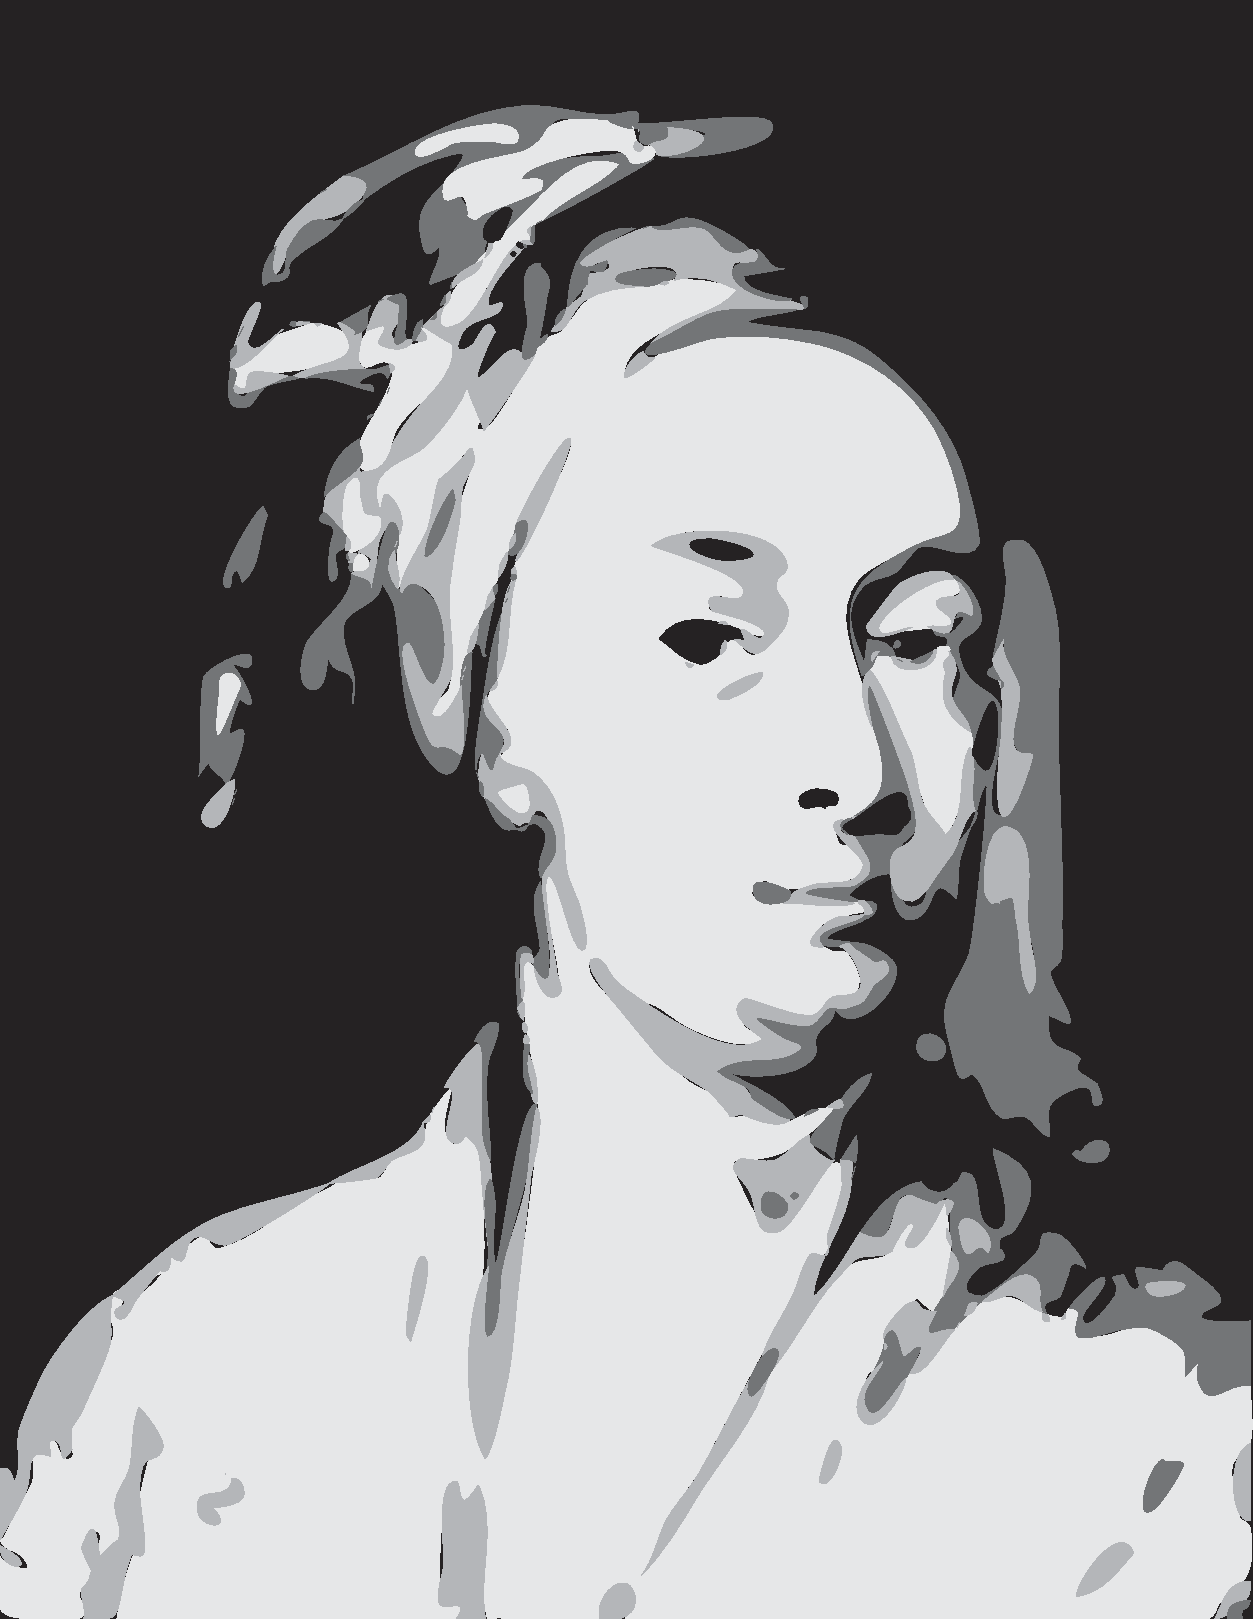
\includegraphics[width=.25\textwidth]{./fotos/calcasdos/Taylor.pdf}\\[5pt]
{\small \bfseries Brook Taylor}
\end{bio}

\begin{theorem}[Taylor]
  \label{teotaylor}\index{teorema!de Taylor}Si $V$ es un espacio de
  Banach, $\Omega $ es un subconjunto abierto de $V$, $u_{0}\in \Omega
  $ y $v\in V$ satisfacen que $u_{0}+tv\in \Omega $ para todo $t\in
  [0,1]$, y $\varphi \in \mathcal{C}^{k+1}(\Omega )$, entonces
  existe $\theta \in (0,1)$ tal que
  \begin{align*}
    \varphi (u_{0}+v) &=\varphi (u_{0})+D\varphi (u_{0})v+\frac{1}{2}D^{2}\varphi (u_{0})[v,v]+\cdots \\
    &\qquad{}+\frac{1}{k!}D^{k}\varphi (u_{0})[\undercbrace{v,\ldots
       ,v}_{\text{$k$ veces}}]
       +\frac{1}{(k+1)!}D^{k+1}\varphi (u_{0}+\theta v)[\undercbrace{v,\ldots ,v}_{\text{$k+1$ veces}}].
  \end{align*}
\end{theorem}

\begin{proof}
  Observa que la función real de variable real $f(t):=\varphi
  (u_{0}+tv)$ está definida en algún intervalo abierto que
  contiene a $[0,1]$, es de clase $\mathcal{C}^{k+1}$ en dicho
  intervalo y
  \begin{equation}
    D^{j}f(t)=D^{j}\varphi (u_{0}+tv)[\undercbrace{v,\ldots ,v}_{\text{$j$ veces}}],\text{\qquad }j=1,\dots,k+1.  \label{tay}
  \end{equation}
  En efecto: por la regla de la cadena, $Df(t)=D\varphi (u_{0}+tv)v$.
  Argumentando por inducción, si $D^{j-1}f(t)=D^{j-1}\varphi
  (u_{0}+tv)[v,\ldots ,v]$ para algún $j=2,\dots,k+1$, entonces
  $D^{j-1}f=\mathcal{E}\circ \left( D^{j-1}\varphi \right) \circ
  \sigma $, donde $\sigma (t):=u_{0}+tv$ y $\mathcal{E}$ es la
  función que a cada $F\in \mathcal{L}_{j-1}(V,\mathbb{R})$ le
  asocia el valor $F[v,\ldots ,v]\in \mathbb{R}$.  Observa que
  $\mathcal{E}$ es lineal y continua [Ejercicio~\ref{eval}].
  Entonces, aplicando la regla de la cadena obtenemos
  \begin{equation*}
    D^{j}f(t)=\left( D^{j}\varphi (u_{0}+tv)v\right)[\undercbrace{v,\ldots ,v}_{\text{$j-1$ veces}}].
  \end{equation*}
  Esta función corresponde a (\ref{tay})\ bajo el isomorfismo
  (\ref{bil}).

  Aplicando el teorema de Taylor para funciones de variable real
  [Ejercicio~\ref{taylorR}] a la función $f$, concluimos que
  existe $\theta \in (0,1)$ tal que
  \begin{align*}
    \varphi (u_{0}+v) &=f(1)=f(0)+Df(0)+\frac{1}{2}D^{2}f(0)+\cdots\\ 
    &\qquad{}+\frac{1}{k!}D^{k}f(0)+\frac{1}{(k+1)!}D^{k+1}f(\theta ) \\
    &=\varphi (u_{0})+D\varphi (u_{0})v+\frac{1}{2}D^{2}\varphi
    (u_{0})[v,v]+\cdots \\
    &\qquad{}+\frac{1}{k!}D^{k}\varphi (u_{0})[\undercbrace{v,\ldots ,v}_{\text{$k$ veces}}]+\frac{1}{(k+1)!}D^{k+1}\varphi (u_{0}+\theta v)[\undercbrace{v,\ldots ,v}_{\text{$k+1$ veces}}].
  \end{align*}
  Esta es la identidad deseada.
\end{proof}

{\abovedisplayskip=7.5pt
\belowdisplayskip=7.5pt
\begin{corollary}[Fórmula de Taylor]
  \index{fórmula!de Taylor}Si $V$ es un espacio de Banach, $\Omega
  $ es un subconjunto abierto de $V$, $u_{0}\in \Omega $ y $\varphi
  \in \mathcal{C}^{k}(\Omega )$, entonces la función
  \begin{equation}
    r_{k}(v):=\varphi (u_{0}+v)-\varphi (u_{0})-D\varphi (u_{0})v-\cdots -\frac{1}{k!}D^{k}\varphi (u_{0})[\undercbrace{v,\ldots ,v}_{\text{$k$ veces}}]  \label{residuo}
  \end{equation}
  está definida en una vecindad de $0$ en $V$ y satisface
  \begin{equation*}
    \lim_{v\rightarrow 0}\frac{r_{k}(v)}{\left\Vert v\right\Vert_{V}^{k}}=0.
  \end{equation*}
\end{corollary}

\begin{proof}
  Sea $\delta >0$ tal que $B_{V}(u_{0},\delta )\subset \Omega $.
  Aplicando el Teorema~\ref{teotaylor} con $k$ en vez de $k+1$
  obtenemos que, para cada $v\in B_{V}(0,\delta )$, existe $\theta
 _{v}\in (0,1)$ tal que
  \begin{equation*}
    \varphi (u_{0}+v)=\sum_{j=0}^{k-1}\frac{1}{j!}D^{j}\varphi
    (u_{0})[v,\ldots ,v]+\frac{1}{k!}D^{k}\varphi (u_{0}+\theta_{v}v)[v,\ldots
    ,v].
  \end{equation*}
  Por otra parte, de la definición de $r_{k}$ se sigue que
  \begin{equation*}
    \varphi (u_{0}+v)=\sum_{j=0}^{k}\frac{1}{j!}D^{j}\varphi
    (u_{0})[v,\ldots ,v]+r_{k}(v).
  \end{equation*}
  Tomando la diferencia de estas identidades obtenemos
  \begin{equation*}
    r_{k}(v)=\frac{1}{k!}\left( D^{k}\varphi (u_{0}+\theta_{v}v)-D^{k}\varphi
      (u_{0})\right) [v,\ldots ,v].
  \end{equation*}
  En consecuencia, si $v\neq 0$,
  \begin{align*}
    \frac{\left\vert r_{k}(v)\right\vert }{\left\Vert v\right\Vert_{V}^{k}} &=\frac{1}{k!}\frac{\left\vert \left( D^{k}\varphi (u_{0}+\theta
         _{v}v)-D^{k}\varphi (u_{0})\right) [v,\ldots ,v]\right\vert }{\left\Vert
        v\right\Vert_{V}^{k}} \\
    &\leq \frac{1}{k!}\left\Vert D^{k}\varphi (u_{0}+\theta_{v}v)-D^{k}\varphi
      (u_{0})\right\Vert_{\mathcal{L}_{k}(V,\mathbb{R})}.
  \end{align*}
  Dado que $D^{k}\varphi \colon \Omega \rightarrow
  \mathcal{L}_{k}(V,\mathbb{R})$ es continua en $u_{0}$ y que $\theta
 _{v}\in (0,1)$, concluimos que $\lim_{v\rightarrow
    0}\frac{r_{k}(v)}{\left\Vert v\right\Vert_{V}^{k}}=0$.
\end{proof}

La función
\begin{equation*}
  P_{k}(v):=\varphi (u_{0})+D\varphi (u_{0})v+\cdots +\frac{1}{k!}D^{k}\varphi
  (u_{0})[\undercbrace{v,\ldots ,v}_{\text{$k$ veces}}]
\end{equation*}
se llama la \textbf{expansión de Taylor de grado }$k$\textbf{\ de
}$\varphi $\textbf{\ alrededor de} $u_{0}$.\index{expansión!de
  Taylor}}

\section{Ejercicios}

\begin{exercise}
  \label{norma}Prueba que
  \begin{equation*}
    \left\Vert T\right\Vert_{\mathcal{L}(V,W)}:=\sup_{\substack{ v\in V  \\ v\neq 0}}\frac{\left\Vert Tv\right\Vert_{W}}{\left\Vert v\right\Vert_{V}}
  \end{equation*}
  es una norma en $\mathcal{L}(V,W)$.
\end{exercise}

\begin{exercise}
  \label{matr}Si identificamos al espacio
  $\mathcal{L}(\mathbb{R}^{n},\mathbb{R}^{m})$ con el espacio
  $\mathcal{M}_{m\times n}(\mathbb{R})$ de matrices de $m\times n$ de
  la manera usual, este espacio resulta isomorfo a
  $\mathbb{R}^{mn}$. Prueba que cualquier isomorfismo de espacios
  vectoriales
  \begin{equation*}
    \iota \colon \mathcal{L}(\mathbb{R}^{n},\mathbb{R}^{m})\rightarrow \mathbb{R}^{mn}
  \end{equation*}
  es un homeomorfismo para cualquier norma que le demos a
  $\mathbb{R}^{mn}$.
\end{exercise}

\begin{exercise}
  Prueba que, para todo $T\in \mathcal{L}(V,W)$,
  \begin{equation*}
    \left\Vert T\right\Vert_{\mathcal{L}(V,W)}=\sup_{v\in \bar{B}_{V}(0,1)}\left\Vert Tv\right\Vert_{W}=\sup_{v\in S_{V}(0,1)}\left\Vert
      Tv\right\Vert_{W}.
  \end{equation*}
  donde $\bar{B}_{V}(0,1):=\left\{v\in V:\left\Vert v\right\Vert_{V}\leq
  1\right\}$ \ y $S_{V}(0,1):=\left\{v\in V:\left\Vert v\right\Vert_{V}=1\right\}$.
\end{exercise}

\begin{exercise}
  \label{normcomp}Sean $V,W,Z$ espacios de Banach. Demuestra las
  siguientes afirmaciones:

  \begin{enumerate}
  \item[(a)] Si $S\in \mathcal{L}(V,W)$ y $T\in \mathcal{L}(W,Z)$
    entonces
    \begin{equation*}
      \left\Vert T\circ S\right\Vert_{\mathcal{L}(V,Z)}\leq \left\Vert
        T\right\Vert_{\mathcal{L}(W,Z)}\left\Vert S\right\Vert_{\mathcal{L}(V,W)}.
    \end{equation*}

  \item[(b)] Si $S_{k}\rightarrow S$ en $\mathcal{L}(V,W)$ y
    $T_{k}\rightarrow T$ en $\mathcal{L}(W,Z)$ entonces $T_{k}\circ
    S_{k}\rightarrow T\circ S$ en $\mathcal{L}(V,Z)$.
  \end{enumerate}
\end{exercise}

\begin{exercise}
  \label{linderi}Prueba que, si $\varphi ,\psi \colon \Omega \rightarrow W$
  son diferenciables en $u_{0}$, entonces $\lambda \varphi +\mu \psi $
  es diferenciable en $u_{0}$ y
  \begin{equation*}
    (\lambda \varphi +\mu \psi )^{\prime }(u_{0})=\lambda \varphi^{\prime
    }(u_{0})+\mu \psi^{\prime }(u_{0}).
  \end{equation*}
\end{exercise}

\begin{exercise}
  \label{inclu}Sean $V_{1},V_{2}$ espacios de Banach,
  $(u_{1},u_{2})\in V_{1}\times V_{2}$. Prueba que las funciones
  \begin{alignat*}{2}
    &\iota_{1,u_{2}} \colon V_{1}\rightarrow V_{1}\times V_{2},&\qquad&\iota
   _{1,u_{2}}(v_{1}):=(v_{1},u_{2}), \\
    &\iota_{2,u_{1}} \colon V_{2}\rightarrow V_{1}\times V_{2},&&\iota
   _{2,u_{1}}(v_{2}):=(u_{1},v_{2}),
  \end{alignat*}
  son diferenciables y calcula su derivada.
\end{exercise}

\begin{exercise}
  Prueba que la función $\ \varphi
  \colon \mathcal{C}^{0}([0,1],V)\rightarrow V\times V$ \ dada por
  \begin{equation*}
    \varphi (\sigma ):=(\sigma (0),\sigma (1))
  \end{equation*}
  es diferenciable y calcula su derivada.
\end{exercise}

\begin{exercise}
  Prueba que la función $\varphi \colon \mathcal{C}^{0}[0,1]\rightarrow
  \mathbb{R}$ dada por
  \begin{equation*}
    \varphi (u):=\int_{0}^{1}u^{2}
  \end{equation*}
  es diferenciable y calcula su derivada.
\end{exercise}

\begin{exercise}
  \emph{Un subconjunto }$A$\emph{\ de un espacio métrico
  }$X$\emph{\ es \textbf{conexo} }\index{conjunto!conexo}\emph{si para
    cualesquiera }$a_{1},a_{2}\in A$\emph{\ existe una trayectoria de
  }$a_{1}$\emph{\ a }$a_{2}$\emph{\ en }$A$.

  Prueba que, si $\Omega $ es un subconjunto abierto y conexo de un
  espacio de Banach $V$, $\varphi \colon \Omega \rightarrow W$ es
  diferenciable en $\Omega $ y $\varphi^{\prime }(u)=0$ para todo
  $u\in \Omega $, entonces $\varphi $ es constante en $\Omega $.
  \emph{(Sugerencia: Usa el teorema del valor medio.)}
\end{exercise}

\begin{exercise}
  Sea $\varphi \colon \mathbb{R}^{2}\rightarrow \mathbb{R}$ dada por
  \begin{equation*}
    \varphi (x,y):=\left\{ 
      \begin{array}{cc}
        \frac{x^{2}y^{2}}{x^{2}+y^{2}} & \text{si }(x,y)\neq (0,0), \\ 
        0 & \text{si }(x,y)=(0,0).
      \end{array}
    \right.
  \end{equation*}
  Prueba que $\varphi $ es diferenciable en $(0,0)$.
  \emph{(Sugerencia: Usa la desigualdad de Young, Lema~\ref{young}.)}
\end{exercise}

\begin{exercise}
  Sea $\varphi \colon \mathbb{R}^{2}\rightarrow \mathbb{R}$ dada por
  \begin{equation*}
    \varphi (x,y):=\left\{ 
      \begin{array}{cc}
        \frac{xy}{x^{2}+y^{2}} & \text{si }(x,y)\neq (0,0), \\ 
        0 & \text{si }(x,y)=(0,0).
      \end{array}
    \right.
  \end{equation*}
  Prueba que existen las derivadas parciales $\frac{\partial \varphi
  }{\partial x}(0,0)$ y $\frac{\partial \varphi }{\partial y}(0,0)$,
  pero que no existe ninguna otra derivada direccional en $(0,0)$, es
  decir, si $xy\neq 0$ no existe el límite
  \begin{equation*}
    \lim_{t\rightarrow 0}\frac{\varphi (tx,ty)-\varphi (0,0)}{t}.
  \end{equation*}
\end{exercise}

\begin{exercise}
  \label{noGdif}Sea $\varphi \colon \mathbb{R}^{2}\rightarrow \mathbb{R}$
  dada por
  \begin{equation*}
    \varphi (x,y):=\left\{ 
      \begin{array}{cc}
        \frac{xy^{2}}{x^{2}+y^{2}} & \text{si }(x,y)\neq (0,0), \\ 
        0 & \text{si }(x,y)=(0,0).
      \end{array}
    \right.
  \end{equation*}
  Prueba que existen todas las derivadas direccionales de $\varphi $
  en $(0,0)$, pero que $\varphi $ no es Gâteaux-diferenciable en
  $(0,0)$.
\end{exercise}

\begin{exercise}
  \label{siGnoF}Prueba que la función $\varphi
  \colon \mathbb{R}^{2}\rightarrow \mathbb{R}$ dada por
  \begin{equation*}
    \varphi (x,y):=\left\{ 
      \begin{array}{cc}
        \frac{x^{3}y}{x^{4}+y^{2}} & \text{si }(x,y)\neq (0,0), \\ 
        0 & \text{si }(x,y)=(0,0).
      \end{array}
    \right.
  \end{equation*}
  es Gâteaux-diferenciable en $(0,0)$, pero no es diferenciable en
  $(0,0)$.
\end{exercise}

\begin{exercise}
  Considera las funciones $f_{1},f_{2},f_{\infty
  }\colon \mathbb{R}^{n}\rightarrow \mathbb{R}$ dadas por
  \begin{equation*}
    f_{1}(x):=\left\Vert x\right\Vert_{1},\text{\qquad }f_{2}(x):=\left\Vert
      x\right\Vert_{2},\text{\qquad }f_{\infty }(x):=\left\Vert x\right\Vert
   _{\infty }.
  \end{equation*}
  Investiga en qué puntos son diferenciables y calcula su derivada
  en dichos puntos.
\end{exercise}

\begin{exercise}
  Considera la función
  \begin{equation*}
    \left\Vert \cdot \right\Vert_{1}\colon \ell_{1}\rightarrow \mathbb{R}\text{,\qquad }\left\Vert x\right\Vert_{1}:=\sum_{k=1}^{\infty
    }\left\vert x_{k}\right\vert .
  \end{equation*}

  \begin{enumerate}
  \item[(a)] Prueba que $\left\Vert \cdot \right\Vert_{1}$\ es
    Gâteaux-diferenciable en $x=(x_{k})$ si y sólo si
    $x_{k}\neq 0$ para todo $k\in \mathbb{N}$. Calcula, en este caso,
    su derivada de Gâteaux.

  \item[(b)] Prueba que $\left\Vert \cdot \right\Vert_{1}$ no es
    Fréchet-diferenciable en ningún punto.
  \end{enumerate}
\end{exercise}

\begin{exercise}
  Sea $f\in \mathcal{C}^{0}[a,b]$. Prueba que la función $\varphi
  \colon (a,b)\rightarrow \mathbb{R}$ dada por
  \begin{equation*}
    \varphi (t):=\int_{t}^{b}f(s)ds
  \end{equation*}
  es de clase $\mathcal{C}^{1}$\ y su derivada es $\varphi^{\prime
  }(t)=-f(t). $
\end{exercise}

\begin{exercise}
  Sea $f\colon [a,b]\times \mathbb{R}\rightarrow \mathbb{R}$ una función
  continua, cuya derivada parcial respecto a la segunda variable
  existe y es continua en $[a,b]\times \mathbb{R}$.

{\abovedisplayskip=9pt 
\belowdisplayskip=9pt 
  \begin{enumerate}
  \item[(a)] Prueba que la función $\varphi
    \colon \mathcal{C}^{0}[a,b]\rightarrow \mathbb{R}$ dada por
    \begin{equation*}
      \varphi (u):=\int_{a}^{b}f(s,u(s))ds
    \end{equation*}
    es de clase $\mathcal{C}^{1}$\ y su derivada está dada por
    \begin{equation*}
      \varphi^{\prime }(u)v=\int_{a}^{b}\partial_{2}f(s,u(s))\left[ v(s)\right]
      ds.
    \end{equation*}

  \item[(b)] Prueba que la función $\Phi
    \colon \mathcal{C}^{0}[a,b]\rightarrow \mathcal{C}^{0}[a,b]$ dada por
    \begin{equation*}
      \Phi (u)(t):=\int_{a}^{t}f(s,u(s))ds
    \end{equation*}
    es de clase $\mathcal{C}^{1}$\ y su derivada está dada por
    \begin{equation*}
      \left( \Phi^{\prime }(u)v\right) (t)=\int_{a}^{t}\partial_{2}f(s,u(s)) 
      \left[ v(s)\right] ds.
    \end{equation*}
  \end{enumerate}}
\end{exercise}

{\abovedisplayskip=9pt 
\belowdisplayskip=9pt 
\begin{exercise}
  \label{derbil}

  \begin{enumerate}
  \item[(a)] Prueba que toda función $T\in \mathcal{L}(V,W)$ es de
    clase $\mathcal{C}^{\infty }$ y calcula su derivada de orden $k$
    para todo $k\in \mathbb{N}$.

  \item[(b)] Prueba que toda función $F\in
    \mathcal{L}(V_{1},V_{2};W)\ $es de clase $\mathcal{C}^{\infty }$ y
    calcula su derivada de orden $k$ para todo $k\in \mathbb{N}$.
  \end{enumerate}
\end{exercise}

\begin{exercise}
  \label{Q}Sea $F\in \mathcal{L}_{2}(V,\mathbb{R})$. Si $F$ es
  simétrica, es decir, si $F[v_{1},v_{2}]=F[v_{2},v_{1}]$ para
  cualesquiera $v_{1},v_{2}\in V$, prueba que la función
  \begin{equation*}
    Q\colon V\rightarrow \mathbb{R}\text{,\qquad }Q(v)=\frac{1}{2}F[v,v],
  \end{equation*}
  es de clase $\mathcal{C}^{\infty }$ y calcula todas sus derivadas.
\end{exercise}

\begin{exercise}
  Prueba que la función $\varphi \colon \mathcal{C}^{0}[0,1]\rightarrow
  \mathcal{C}^{0}[0,1]$ dada por $\varphi (u):=u^{2}$ es de clase
  $\mathcal{C}^{\infty } $ y calcula todas sus derivadas.
\end{exercise}

\begin{exercise}
  Sea $K\colon [a,b]\times [a,b]\rightarrow \mathbb{R}$ una
  función continua y simétrica. Prueba que la función
  $\varphi \colon \mathcal{C}^{0}[a,b]\rightarrow \mathbb{R}$ dada por
  \begin{equation*}
    \varphi (u):=\int_{a}^{b}\int_{a}^{b}K(x,y)u(x)u(y)dxdy
  \end{equation*}
  es de clase $\mathcal{C}^{\infty }$ y calcula todas sus derivadas.
\end{exercise}}

\begin{exercise}
  \label{eval}Sean $V_{1},\dots,V_{n},W$ espacios de Banach y $v_{j}\in
  V_{j}$. Prueba que la función
  \begin{equation*}
    \mathcal{E}\colon \mathcal{L}(V_{1},\dots,V_{n};W)\rightarrow W,\qquad \mathcal{E}(F):=F[v_{1},\ldots ,v_{n}],
  \end{equation*}
  es lineal y continua.
\end{exercise}

\begin{exercise}
  \label{multi}Considera la función $\iota
  \colon \mathcal{L}(V_{1},V_{2};W)\rightarrow
  \mathcal{L}(V_{1},\mathcal{L}(V_{2},W))$ dada por $\iota
  (F):=\hat{F}$ donde
  \begin{equation*}
    (\hat{F}v_{1})v_{2}=F[v_{1},v_{2}],\qquad \forall v_{1}\in V_{1},\text{ }v_{2}\in V_{2}.
  \end{equation*}
  Prueba que

  \begin{enumerate}
  \item[(a)] $\iota $ está bien definida, es decir, $\hat{F}\in
    \mathcal{L}(V_{1},\mathcal{L}(V_{2},W))$ si $F\in
    \mathcal{L}(V_{1},V_{2};W)$,

  \item[(b)] $\iota $ es un isomorfismo de espacios vectoriales,

  \item[(c)] $\iota $ es una isometría, es decir,
    \begin{equation*}
      \left\Vert F\right\Vert_{\mathcal{L}(V_{1},V_{2};W)}=\left\Vert \hat{F}\right\Vert_{\mathcal{L}(V_{1},\mathcal{L}(V_{2},W))}\qquad \forall F\in 
      \mathcal{L}(V_{1},V_{2};W).
    \end{equation*}
  \end{enumerate}
\end{exercise}

\begin{exercise}
  Sean $V_{1},\dots,V_{n},W$ espacios de Banach, $\Omega $ un
  subconjunto abierto de $V:=V_{1}\times \cdots \times V_{n}$ y
  $\varphi \colon \Omega \rightarrow W$.

  \begin{enumerate}
  \item[(a)] Prueba que si $\varphi $ es de clase $\mathcal{C}^{2}$
    entonces existen las derivadas parciales de orden~$2$,
    \begin{equation*}
      \partial_{j}\partial_{i}\varphi (u):=\partial_{j}\left( \partial
       _{i}\varphi \right) (u)\in \mathcal{L}(V_{j},\mathcal{L}(V_{i},W))\cong 
      \mathcal{L}(V_{j},V_{i};W),
    \end{equation*}
    para cualesquiera $u\in \Omega $, $i,j=1,\ldots ,n$, y que se
    cumple
    \begin{equation*}
      D^{2}\varphi (u)[v,w]=\sum_{i,j=1}^{n}\partial_{j}\partial
     _{i}\varphi (u)[v_{j},w_{i}]
    \end{equation*}
    para cualesquiera $v=(v_{1},\ldots ,v_{n})$, $w=(w_{1},\ldots
    ,w_{n})\in V$.

  \item[(b)] Prueba que, si $\varphi $ es de clase $\mathcal{C}^{2}$,
    entonces $\partial_{j}\partial_{i}\varphi (u)=\partial
   _{i}\partial_{j}\varphi (u)$ para cualesquiera $u\in \Omega $,
    $i,j=1,\ldots ,n$.

  \item[(c)] Prueba que, si las derivadas parciales $\partial
   _{j}\partial_{i}\varphi \colon \Omega \rightarrow
    \mathcal{L}(V_{j},V_{i};W)$ de orden $2$ existen y son continuas
    para cualesquiera $i,j=1,\ldots ,n$, entonces $\varphi $ es de
    clase $\mathcal{C}^{2}$.

  \item[(d)] Formula y demuestra los resultados análogos para
    $\varphi $ de clase $\mathcal{C}^{k}$, $k\geq 2$.
  \end{enumerate}
\end{exercise}

\begin{exercise}[Teorema de Taylor para funciones de variable real]
  \label{taylorR}Prueba que si $f\in \mathcal{C}^{k+1}(a,b)$ y $0\in
  (a,b)$ entonces, para cada $t\in (a,b)$, existe un punto $\theta \in
  (0,1)$ tal que
  \begin{equation*}
    f(t)=f(0)+Df(0)t+\frac{1}{2}D^{2}f(0)t^{2}+\cdots +\frac{1}{k!}D^{k}f(0)t^{k}+\frac{1}{(k+1)!}D^{k+1}f(\theta t)t^{k+1}.
  \end{equation*}
\end{exercise}

\begin{exercise}
  Sea $Q\colon V\rightarrow \mathbb{R}$ como en el \emph{Ejercicio~\ref{Q}}.

  \begin{enumerate}
  \item[(a)] Para cualesquiera $k\geq 2$ y $u_{0}\in V$, calcula la
    expansión de Taylor de grado $k$\ de $Q$\ alrededor de
    $u_{0}$.

  \item[(b)] Calcula la función $r_{k}$ definida en
    \emph{(\ref{residuo})}.
  \end{enumerate}
\end{exercise}

\begin{exercise}
  Sea $\Omega :=\left\{(x,y)\in \mathbb{R}^{2}:x+y\neq 0\right\}$ y sea $\varphi
  \colon \Omega \rightarrow \mathbb{R}$ la función dada por
  \begin{equation*}
    \varphi (x,y):=\frac{x-y}{x+y}.
  \end{equation*}

  \begin{enumerate}
  \item[(a)] Calcula la expansión de Taylor de grado $2$ de la
    función $\varphi $ alrededor de $(1,1)$.

  \item[(b)] Comprueba directamente que la función $r_{2}$
    definida en \emph{(\ref{residuo})} con $u_{0}=(1,1)$ satisface
    \begin{equation*}
      \lim_{(x,y)\rightarrow (1,1)}\frac{r_{2}(x,y)}{x^{2}+y^{2}}=0.
    \end{equation*}
  \end{enumerate}
\end{exercise}

\begin{exercise}
  Utiliza una expansión de Taylor de la función $\varphi
  (x,y):=\cos (x+y)$ para calcular
  \begin{equation*}
    \lim_{(x,y)\rightarrow (0,0)}\frac{1-\cos (x+y)}{\sqrt{x^{2}+y^{2}}}.
  \end{equation*}
\end{exercise}

\chapter{El teorema de la función implícita}

\label{captfi}Sean $\varphi \colon \Omega \rightarrow \mathbb{R}$ una
función de clase $\mathcal{C}^{1}$ definida en un abierto $\Omega
$ de $\mathbb{R}^{n}$, y $c\in \mathbb{R}$. Queremos obtener
información sobre la estructura del conjunto de soluciones $\xi
\in \Omega $ de la ecuación
\begin{equation}
  \varphi (\xi )=c,  \label{ec}
\end{equation}
al que denotaremos por
\begin{equation*}
  M:=\left\{\xi \in \Omega :\varphi (\xi )=c\right\}.
\end{equation*}

Veamos un ejemplo. Si $\varphi \colon \mathbb{R}^{2}\rightarrow \mathbb{R}$
es la función $\varphi (x,y)=x^{2}-y^{2}$ entonces para $c<0$ el
conjunto $M$ tiene dos componentes: una de ellas es la gráfica de
la función $x\mapsto \sqrt{x^{2}-c}$ y la otra es la gráfica
de $x\mapsto -\sqrt{x^{2}-c}$. Análogamente, si $c>0$, el conjunto
$M$ tiene dos componentes: la gráfica de la función $y\mapsto
\sqrt{c+y^{2}}$ y la de la función $y\mapsto -\sqrt{c+y^{2}}$. En
cambio, si $c=0$, no existe ninguna vecindad de $(0,0)$ en
$\mathbb{R}^{2}$ cuya intersección con $M$ sea la gráfica de
alguna función.
\begin{figure}[htb]
  \centering
  \begin{tikzpicture}[scale=.5]
  \draw (-3.2,0)--(3.2,0);
  \draw (0,-3.2)--(0,3.2);

  \draw[very thick] plot[samples=100, domain=-3:3](\x, {((\x)^2 + 1)^(1/2)});
  \draw[very thick] plot[samples=100, domain=-3:3](\x, {-((\x)^2 + 1)^(1/2)});
  \draw (0,-3.4) node[below] {$x^2-y^2=c<0$};
  
%   \foreach \x in {0.5, 1}{
%                \draw[thin] (\x,-0.025)--(\x,0.025);
%                \draw[thin] (-.025,\x)--(0.025,\x);
% };
  % \draw (0,-.025) node[below] {$0$};
  % \draw (.5,-.025) node[below] {$\frac{1}{2}$};
  % \draw (1,-.025) node[below] {$1$};
  % \draw (-.025,.5) node[left] {$\frac{1}{2}$};
  % \draw (-.025,1) node[left] {$1$};
\end{tikzpicture}
\qquad
  \begin{tikzpicture}[scale=.5]
  \draw (-3.2,0)--(3.2,0);
  \draw (0,-3.2)--(0,3.2);

  \draw[very thick] plot[samples=100, domain=-3:3]({((\x)^2 +
    1)^(1/2)}, \x);
  \draw[very thick] plot[samples=100, domain=-3:3]({-((\x)^2 +
    1)^(1/2)}, \x);
  \draw (0,-3.4) node[below] {$x^2-y^2=c>0$};
  
%   \foreach \x in {0.5, 1}{
%                \draw[thin] (\x,-0.025)--(\x,0.025);
%                \draw[thin] (-.025,\x)--(0.025,\x);
% };
  % \draw (0,-.025) node[below] {$0$};
  % \draw (.5,-.025) node[below] {$\frac{1}{2}$};
  % \draw (1,-.025) node[below] {$1$};
  % \draw (-.025,.5) node[left] {$\frac{1}{2}$};
  % \draw (-.025,1) node[left] {$1$};
\end{tikzpicture}
\qquad
  \begin{tikzpicture}[scale=.5]
  \draw (-3.2,0)--(3.2,0);
  \draw (0,-3.2)--(0,3.2);

  \draw[very thick] plot[samples=100, domain=-3:3](\x, \x);
  \draw[very thick] plot[samples=100, domain=-3:3](\x, -\x);
  \draw (0,-3.4) node[below] {$x^2-y^2=0$};
  
%   \foreach \x in {0.5, 1}{
%                \draw[thin] (\x,-0.025)--(\x,0.025);
%                \draw[thin] (-.025,\x)--(0.025,\x);
% };
  % \draw (0,-.025) node[below] {$0$};
  % \draw (.5,-.025) node[below] {$\frac{1}{2}$};
  % \draw (1,-.025) node[below] {$1$};
  % \draw (-.025,.5) node[left] {$\frac{1}{2}$};
  % \draw (-.025,1) node[left] {$1$};
\end{tikzpicture}

  % \caption{}\label{fig:10.1}
\end{figure}

Nota que $\nabla \varphi (x,y)\neq (0,0)$ si $(x,y)\neq (0,0)$. En
este caso, la recta perpendicular a $\nabla \varphi (x,y)$ es tangente
a $M$ en el punto $(x,y),\ $es decir, $M$ se parece a dicha recta en
una vecindad del punto.

Los conjuntos $M$ de soluciones de (\ref{ec}) que tienen la propiedad
de que $\nabla \varphi (\xi )\neq 0$ para todo $\xi \in M$ se llaman
\emph{variedades}. El teorema de la función implícita asegura
que, si $M$ es una variedad entonces, en una vecindad de cada punto
$\xi \in M$, $\ M$ es la gráfica de una función cuyo dominio
es un abierto en el subespacio de $\mathbb{R}^{n}$ ortogonal a $\nabla
\varphi (\xi )$ y cuyo codominio es el espacio generado por $\nabla
\varphi (\xi )$.
\begin{figure}[htb]
  \centering
  \begin{tikzpicture}[scale=.6]
%  \draw[thin,fill=gray!25] plot[smooth cycle, tension=.85]
  \draw[thick] plot[smooth cycle, tension=.85]
  coordinates{(1.4,-2) (-1.4,-2) (-2.2,1.3) (2,2) (0,0) (2,-.5)};
%  coordinates{(-1,-2) (1,-2) (1.7,1.3) (-1,2) (-1,0.5) (0,.3)};
\draw[mark=*, mark size=1.2pt] plot coordinates{(-0.19,-2.44)};
\draw[very thin] (-2.39,-2.44)--(2.01,-2.44);
\draw[very thin] (-0.19,-4.64)--(-0.19,-0.24);
\draw[very thick, -latex'] (-0.19,-2.44)--(-0.19,-1);
\draw[dashed] (-2.19,-4.44) rectangle (1.81,-0.44);
\node[right] at (-0.2,-1.2) {$\nabla\varphi(\xi)$};
\node[below] at (0,-2.44) {$\xi$};
\node[right] at (2,1.8) {$M$};
\end{tikzpicture}

  % \caption{}\label{fig:10.2}
\end{figure}

En particular, cerca de $\xi $, $M$ se parece a $\mathbb{R}^{n-1}$.
Esto permite extender conceptos y resultados del cálculo
diferencial a las variedades.

En las aplicaciones interesa a menudo encontrar mínimos o
máximos locales de una cierta función $g\colon \Omega \rightarrow
\mathbb{R}$ sobre una variedad $M$. El teorema de la función
implícita proporciona un criterio sencillo para detectarlos: si
$\xi \in M$ es un máximo o un mínimo local de $g$ en $M$,
entonces $\nabla g(\xi )$ es perpendicular al espacio tangente a $M$
en $\xi $. Por ejemplo, si $g(x,y,z):=z$ es la función que a cada
punto de $\mathbb{R}^{3}$ le asocia su altura respecto al plano $xy$,
los máximos y mínimos locales de $g$ sobre una superficie $M$
en $\mathbb{R}^{3}$ tienen la propiedad de que el plano tangente a $M$
en tales puntos es paralelo al plano $xy$.
\begin{figure}[htb]
  \centering
  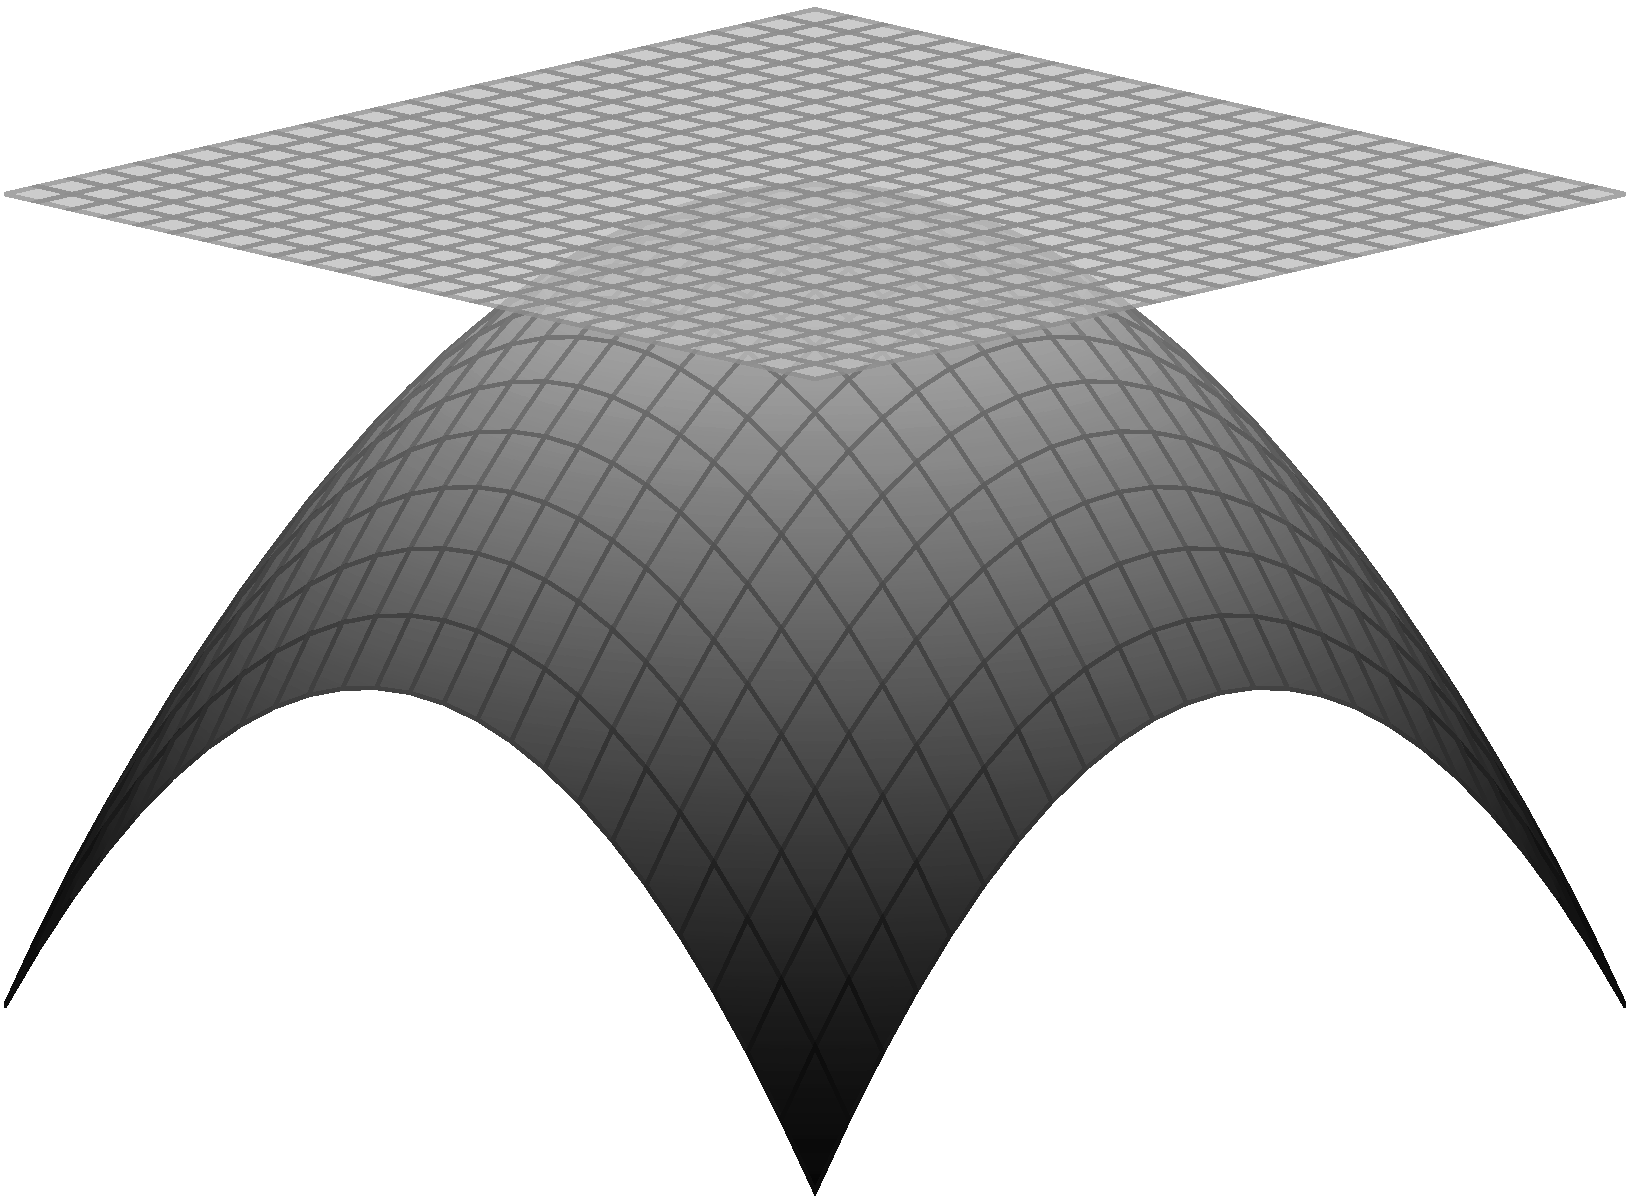
\includegraphics{./paraboloide-crop.png}
%  \begin{tikzpicture} 
  \begin{axis}[ view/az=45,
    view/el=15,
    axis lines=none,
    colormap={bw}{gray(0cm)=(0); gray(1cm)=(0.8)}]
    \addplot3[surf,domain=-1:1,y domain=-1:1, shader=faceted interp] {-(x^2+y^2)};
    \addplot3[surf,domain=-1:1,y domain=-1:1,opacity=.8] {0};    
  \end{axis} 
\end{tikzpicture}

  % \caption{}\label{fig:10.3}
\end{figure}

Los resultados anteriores son válidos también en espacios de
Banach y tienen aplicaciones importantes en ese contexto, por ejemplo,
para probar la existencia de soluciones de ciertas ecuaciones
diferenciales no lineales\footnote{%
Consulta, por ejemplo,~\cite{Ambrosetti}.}.

\section{El teorema de la función implícita}

Sean $Y$ un espacio de Banach, $\Omega $ un subconjunto abierto de
$Y$, $\varphi \colon \Omega \rightarrow \mathbb{R}^{m}$ una función de
clase $\mathcal{C}^{1}$ y $c\in \mathbb{R}^{m}$. Como mencionamos en
la introducción, nos interesa obtener información sobre la
estructura del conjunto de soluciones $u\in \Omega $ de la
ecuación
\begin{equation}
  \varphi (u)=c,  \label{ecua}
\end{equation}
al que denotaremos por
\begin{equation*}
  M:=\left\{u\in \Omega :\varphi (u)=c\right\}.
\end{equation*}
Veamos el siguiente ejemplo.

\begin{example}
  \label{ejesfera}Sea $\varphi \colon \mathbb{R}^{n}\rightarrow \mathbb{R}$
  la función $\varphi (x_{1},\ldots ,x_{n})=x_{1}^{2}+\cdots
  +x_{n}^{2}$. Si $c>0$, el conjunto $M$ es la esfera de radio
  $\sqrt{c}$ con centro en el origen.  Ésta tiene la propiedad de
  que, localmente, se parece a $\mathbb{R}^{n-1} $ en el siguiente
  sentido: Para cada punto $\xi \in M$ existe un subespacio vectorial
  $T_{\xi }M$ de $\mathbb{R}^{n}$ de dimensión $n-1$, a saber
  \begin{equation*}
    T_{\xi }M:=\left\{y\in \mathbb{R}^{n}:y\cdot \xi =0\right\},
  \end{equation*}
  tal que, en una vecindad de $\xi $, el conjunto $M$ es la
  gráfica de una función de clase $\mathcal{C}^{\infty }$ cuyo
  dominio es la bola abierta de radio $\sqrt{c}$ en $T_{\xi }M$ y cuyo
  codominio es el complemento ortogonal de $T_{\xi }M$.
  Dicha función $f$ está dada por
  \begin{equation*}
    f(y):=\Bigl( \sqrt{c-\Vert y\Vert^{2}}\Bigr) \frac{\xi }{\left\Vert \xi \right\Vert },\text{\qquad }\forall y\in T_{\xi }M\text{ tal
      que }\left\Vert y\right\Vert <\sqrt{c}.
  \end{equation*}
  La gráfica de $f$, definida como
  \begin{equation*}
    \text{\emph{graf}}(f):=\left\{(y,z):y\in T_{\xi }M,\text{ }\left\Vert
      y\right\Vert <\sqrt{c},\text{ }z=f(y)\right\},
  \end{equation*}
  resulta ser el conjunto $\left\{x\in M:x\cdot \xi >0\right\}$, el cual es
  abierto en $M$ y contiene a $\xi $.
\begin{figure}[htb]
  \centering
  \begin{tikzpicture}[scale=.4]
%  \draw[very thin,scale=1.3] (-3,4) -- (5,-1);
%  \draw[very thin,scale=1.4] (-2.2,3.5) -- (4.2,-0.5);
  \draw[very thin,scale=1.4] (-1.8,3.25) -- (3.8,-0.25);

  \draw[fill={white}, fill opacity=0.95] (0,0) circle ({sqrt(13)});
%  \draw[very thin,scale=1.3] (5,-1) -- (3,-4) -- (-5,1) -- (-3,4) -- cycle;
%  \draw[very thin,scale=1.4] (4.2,-0.5) -- (3,-4) -- (-5,1) --
  \draw[very thin,scale=1.4] (3.8,-0.25) -- (3,-4) -- (-5,1) --
  (-1.8,3.25);

  \draw[thick,-latex'] (0,0) -- (2,3);
  \draw (.2,.3) -- (.5,.1) -- (.3,-.2);

  \draw[dashed, cm={cos(33.7), -sin(33.7), sin(33.7), cos(33.7), (0,0)}]
  (0,0) ellipse ({0.38*sqrt(89)} and {0.38*sqrt(13)});

  \draw (2.3,2.9) node[above] {$\xi$};
  \draw[scale=1.3] (3.6,-2.5) node[right] {$T_\xi M$};

\end{tikzpicture} 

  % \caption{}\label{fig:10.4}
\end{figure}

  Observa que $\nabla \varphi (\xi )=2\xi $, por lo que $T_{\xi
  }M=\left\{y\in \mathbb{R}^{n}:y\cdot \nabla \varphi (\xi )=0\right\}$.
\end{example}

Queremos obtener una condición suficiente para que el conjunto de
soluciones de la ecuación (\ref{ecua}) sea, localmente, la
gráfica de una función. El siguiente concepto jugará un
papel fundamental.

\begin{definition}
  Decimos que $c\in \mathbb{R}^{m}$ es un \textbf{valor regular de}
  $\varphi \colon \Omega \rightarrow \mathbb{R}^{m}$ \index{valor!regular}si
  $\varphi^{\prime }(u)\colon Y\rightarrow \mathbb{R}^{m}$ es suprayectiva
  para todo $u\in M:=\left\{w\in \Omega :\varphi (w)=c\right\}$.

  El subespacio vectorial
  \begin{equation*}
    T_{u}M:=\ker \varphi^{\prime }(u)=\left\{v\in Y:\varphi^{\prime }(u)v=0\right\}
  \end{equation*}
  de $Y$ se llama el \textbf{espacio tangente a} $M$
  \index{espacio!tangente}en el punto $u\in M$.
\end{definition}

Nota que, si $M=\emptyset $, entonces $c$ es un valor regular de
$\varphi $.  Si $c$ es un valor regular de $\varphi $ y $M\neq
\emptyset $, necesariamente $\dim Y\geq m$. Observa además que,
dado que $\varphi^{\prime }(u)\colon Y\rightarrow \mathbb{R}^{m}$ es
continua, el espacio tangente $T_{u}M$ es un subespacio cerrado de $Y$
y, por tanto, es un espacio de Banach.

\begin{example}
  Si $\Omega $ es un subconjunto abierto de $\mathbb{R}^{n}$\ y
  $\varphi \colon \Omega \rightarrow \mathbb{R}$ es de clase
  $\mathcal{C}^{1}$\ entonces $c$ es un valor regular de $\varphi $ si
  y sólo si $\nabla \varphi (\xi )\neq 0$ para cada $\xi \in M$.
  En este caso,
  \begin{equation*}
    T_{\xi }M=\left\{y\in \mathbb{R}^{n}:y\cdot \nabla \varphi (\xi )=0\right\},
  \end{equation*}
  es decir, $T_{\xi }M$\ es el subespacio ortogonal a $\nabla \varphi
  (\xi )$.
\end{example}

Este ejemplo incluye a la función $\varphi (x_{1},\ldots
,x_{n})=x_{1}^{2}+\cdots +x_{n}^{2}$, considerada en el Ejemplo
\ref{ejesfera}, y es un caso particular del siguiente ejemplo.

\begin{example}
  \label{tangRn}Si $\Omega $ es un subconjunto abierto de
  $\mathbb{R}^{n}$\ y $\varphi =(\varphi_{1},\dots,\varphi_{m})\colon \Omega
  \rightarrow \mathbb{R}^{m}$ es de clase $\mathcal{C}^{1}$, $m\leq
  n$,\ entonces $c$ es un valor regular de $\varphi $ si y sólo si
  el conjunto
  \begin{equation*}
    \left\{ \nabla \varphi_{1}(\xi ),\ldots ,\nabla \varphi_{m}(\xi )\right\}
  \end{equation*}
  es linealmente independiente para cada $\xi \in M$. En ese caso,
  \begin{equation*}
    T_{\xi }M=\left\{y\in \mathbb{R}^{n}:y\cdot \nabla \varphi_{j}(\xi )=0,\text{ }j=1,\ldots ,m\right\}
  \end{equation*}
  es el complemento ortogonal del espacio generado por $\left\{ \nabla
    \varphi_{1}(\xi ),\ldots ,\nabla \varphi_{m}(\xi )\right\} $.
\end{example}

\begin{proof}
  En efecto, $\varphi^{\prime }(\xi )$ es la función lineal dada
  por la matriz jacobiana
  \begin{equation*}
    \varphi^{\prime }(\xi )=\left( 
      \begin{array}{ccc}
        \frac{\partial \varphi_{1}}{\partial x_{1}}(\xi ) & \cdots & \frac{\partial
          \varphi_{1}}{\partial x_{n}}(\xi ) \\ 
        \vdots &  & \vdots \\ 
        \frac{\partial \varphi_{m}}{\partial x_{1}}(\xi ) & \cdots & \frac{\partial
          \varphi_{m}}{\partial x_{n}}(\xi )
      \end{array}
    \right) ,
  \end{equation*}
  y ésta es suprayectiva si y sólo si la matriz tiene rango
  máximo, es decir, sí y sólo si sus renglones son
  linealmente independientes. 

  Nota que
  $\varphi^{\prime }(\xi )y=\left( \nabla \varphi_{1}(\xi )\cdot
    y,\ldots ,\nabla \varphi _{m}(\xi )\cdot y\right) $,
  así que $y\in T_{\xi }M$ si y sólo si
  $\nabla \varphi_{j}(\xi )\cdot y=0$ para todo $j=1,\ldots ,m$.
\end{proof}

Si queremos expresar localmente a $M$ como la gráfica de una
función definida en un subconjunto abierto del espacio tangente,
necesitamos primero expresar a $Y$ como un producto de espacios de
Banach de la forma $T_{u}M\times W_{u}$. Si $Y=\mathbb{R}^{n}$ podemos
simplemente tomar a $W_{u} $ como el complemento ortogonal de
$T_{u}M$.

Desde un punto de vista puramente algebraico, todo subespacio $V$ de
un espacio vectorial $Y$ tiene un espacio complementario, es decir,
existe un subespacio $W$ de $Y$ tal que $Y$ es linealmente isomorfo a
$V\times W$. Sin embargo, si $Y$ es un espacio de Banach de
dimensión infinita y $V$ es cerrado en $Y$, ni $W$ es
necesariamente cerrado en $Y$, ni $Y$ es necesariamente homeomorfo a
$V\times W$.

En el caso particular que estamos considerando sí podemos
expresar a $Y$ como $T_{u}M\times W_{u}$ de manera apropiada. Se tiene
el siguiente resultado.

\begin{proposition}
  \label{complemento}Si $Y$ es un espacio de Banach, $T\in
  \mathcal{L}(Y,\mathbb{R}^{m})$ es suprayectiva y $V:=\ker T$,
  entonces existe un subespacio vectorial cerrado $W$ de $Y$ tal que
  la restricción $T\mid_{W}\colon W\rightarrow \mathbb{R}^{m}$ de $T$ a
  $W$ es un isomorfismo de espacios vectoriales y la función
  lineal
  \begin{equation*}
    \iota \colon V\times W\rightarrow Y,\text{\qquad }\iota (v,w):=v+w,
  \end{equation*}
  es un homeomorfismo.
\end{proposition}

\begin{proof}
  Sea $\left\{e_{1},\ldots ,e_{m}\right\}$ la base canónica de
  $\mathbb{R}^{m}$. Escogemos $w_{j}\in Y$ tal que $Tw_{j}=e_{j}$,
  $j=1,\dots,m$, y denotamos por $W$ al subespacio vectorial de $Y$
  generado por $\left\{w_{1},\ldots ,w_{m}\right\}$. La función lineal
  $S\colon \mathbb{R}^{m}\rightarrow Y$ dada por
  \begin{equation*}
    S(x_{1},\dots,x_{m}):=x_{1}w_{1}+\cdots +x_{m}w_{m}
  \end{equation*}
  es también continua, ya que su dominio es de dimensión
  finita (ver Ejercicio~\ref{ejnorfinequiv}). Además, cumple que
  $TSx=x$ para todo $x\in \mathbb{R}^{m}$. En consecuencia, $y-STy\in
  \ker T$ para todo $y\in Y$ y la función
  \begin{equation*}
    \pi \colon Y\rightarrow V\times W,\text{\qquad }\pi (y):=(y-STy,STy),
  \end{equation*}
  es lineal y continua (ver Ejercicio~\ref{distcont}). Claramente,
  $\iota $ es lineal y continua y $\iota \circ \pi =\id_{Y}$. Observa
  que $ST(v+w)=STw=w$ para todo $v\in V$, $w\in W$. Por tanto,
  \begin{equation*}
    \pi (\iota (v,w))=(v+w-ST(v+w),\,ST(v+w))=(v,w),
  \end{equation*}
  es decir, $\pi \circ \iota =\id_{V\times W}$. Esto prueba que $\iota
  $ es un homeomorfismo.

  Para probar que $W$ es cerrado en $Y$ tomemos una sucesión
  $(y_{k})$ en $W$ tal que $y_{k}\rightarrow y$ en $Y$. Como $ST$ es
  continua, se tiene que $y_{k}=STy_{k}\rightarrow STy$. En
  consecuencia, $y=STy\in W$. Esto prueba que $W$ es cerrado en $Y$.
\end{proof}

\begin{definition}
  \label{defisoBanach}Una función lineal y biyectiva
  $T\colon V\rightarrow W$ entre dos espacios de Banach $V$ y $W$ que es
  además un homeomorfismo se llama un \textbf{isomorfismo de
    Banach}.  \index{isomorfismo!de Banach}
\end{definition}

De la Proposición~\ref{complemento} se desprende que, si $c$ es un
valor regular de $\varphi $ entonces, para cada $u\in M$, existe un
subespacio cerrado $W_{u}$ de $Y$ tal que la función
\begin{equation*}
  \iota \colon T_{u}M\times W_{u}\rightarrow Y,\text{\qquad }\iota (v,w):=v+w,
\end{equation*}
es un isomorfismo de Banach. El teorema de la función implícita,
que enunciaremos a continuación, garantiza que $M$ se puede
expresar localmente como la gráfica de una función cuyo
dominio es un abierto de $T_{u}M$ y cuyo codominio es $W_{u}$.

\begin{theorem}[de la función implícita]
  \label{teofi}\index{teorema!de la función implícita}Sean
  $V,W,Z$ espacios de Banach, $\Omega \ $un subconjunto abierto de
  $V\times W$, $(v_{0},w_{0})\in \Omega $ y $\varphi \colon \Omega
  \rightarrow Z$ una función de clase $\mathcal{C}^{1}$ en $\Omega
  $. Si $\varphi (v_{0},w_{0})=c$ y $\partial_{2}\varphi
  (v_{0},w_{0})\in \mathcal{L}(W,Z)$ es un isomorfismo de Banach,
  entonces existen $\delta ,\eta >0$ tales que $B_{V}(v_{0},\delta
  )\times B_{W}(w_{0},\eta )\subset \Omega $ y una función
  $f\colon B_{V}(v_{0},\delta )\rightarrow W$ de clase $\mathcal{C}^{1}$ con
  las siguientes propiedades:

  \begin{enumerate}
  \item[(I) \ ] El conjunto de soluciones $(v,w)\in B_{V}(v_{0},\delta
    )\times B_{W}(w_{0},\eta )$ de la ecuación
    \begin{equation*}
      \varphi (v,w)=c
    \end{equation*}
    coincide con la gráfica de $f$,
    \begin{equation*}
      \text{\emph{graf}}(f):=\left\{(v,f(v)):v\in B_{V}(v_{0},\delta )\right\}.
    \end{equation*}
    En particular, $f(v_{0})=w_{0}$ y $f(v)\in B_{W}(w_{0},\eta )$
    para todo $v\in B_{V}(v_{0},\delta )$.

  \item[(II) ] Para todo $v\in B_{V}(v_{0},\delta )$ se cumple
    que$\ \partial_{2}\varphi (v,f(v))$ es un isomorfismo de Banach y
    \begin{equation*}
      f^{\prime }(v)=-\left[ \partial_{2}\varphi (v,f(v))\right]^{-1}\circ
      \partial_{1}\varphi (v,f(v)).
    \end{equation*}
  \end{enumerate}
\end{theorem}

Pospondremos la demostración de este teorema para la Sección
\ref{sec:demtfi} de este capítulo, y procederemos a presentar
algunas consecuencias importantes.

La Proposición~\ref{complemento} asegura que, si $c\in
\mathbb{R}^{m}$ es un valor regular de $\varphi \colon \Omega \rightarrow
\mathbb{R}^{m}$, entonces para cada $u\in M$ existe un subespacio
cerrado $W_{u}$ de $Y$ tal que la función
\begin{equation*}
  \iota \colon T_{u}M\times W_{u}\rightarrow Y,\text{\qquad }\iota (v,w):=v+w,
\end{equation*}
es un isomorfismo de Banach. Identificando a $Y$ con $T_{u}M\times
W_{u}$ mediante dicho isomorfismo, se obtiene que $\partial
_{2}\varphi (u)\equiv \varphi^{\prime }(u)\mid
_{W_{u}}\colon W_{u}\rightarrow \mathbb{R}^{m}$ es un isomorfismo. Nota que
$W_{u}$ no es único. Para cualquier elección de $W_{u}$ con
las propiedades mencionadas se tiene el siguiente resultado, que es
consecuencia inmediata del teorema de la función implícita.

\begin{corollary}
  \label{variedad}Si $c\in \mathbb{R}^{m}$ es un valor regular de
  $\varphi \colon \Omega \rightarrow \mathbb{R}^{m}$ y $u=v_{0}+w_{0}\in M$
  con $v_{0}\in T_{u}M$ y $w_{0}\in W_{u}$, entonces existen $\delta
  ,\eta >0$ y una función $f\colon B_{T_{u}M}(v_{0},\delta )\rightarrow
  W_{u}$ de clase $\mathcal{C}^{1}$ tal que
  \begin{equation*}
    M\cap \left( B_{T_{u}M}(v_{0},\delta )\times B_{W_{u}}(w_{0},\eta )\right)
    =\left\{v+f(v):v\in B_{T_{u}M}(v_{0},\delta )\right\}.
  \end{equation*}
  Más aún, $\partial_{2}\varphi (v+f(v))$ es un isomorfismo y
  \begin{equation*}
    f^{\prime }(v)=-\left[ \partial_{2}\varphi (v+f(v))\right]^{-1}\circ
    \partial_{1}\varphi (v+f(v))
  \end{equation*}
  para cada $v\in B_{T_{u}M}(v_{0},\delta )$.
\end{corollary}

Es importante hacer notar que, si la función $\varphi $ del
Teorema~\ref{teofi} y del Corolario~\ref{variedad}\ es de clase
$\mathcal{C}^{k}$, entonces la función $f$ también es de clase
$\mathcal{C}^{k}$ [Ejercicio~\ref{fiCk}].

\section{Extremos locales de una función diferenciable sobre una
  variedad}

Sean $\Omega $ un subconjunto abierto de un espacio de Banach $Y$,
$\varphi \colon \Omega \rightarrow \mathbb{R}^{m}$ una función de clase
$\mathcal{C}^{1} $, $c\in \mathbb{R}^{m}$ y $M:=\left\{u\in \Omega :\varphi
(u)=c\right\}$. El Corolario~\ref{variedad} permite caracterizar al espacio
tangente como sigue.

{\abovedisplayskip=8pt
\belowdisplayskip=8pt
\begin{proposition}
  Si $c$ es un valor regular de $\varphi $ entonces, para cada $u\in
  M$,
  \begin{equation*}
    T_{u}M=\left\{\sigma^{\prime }(0):\sigma \in \Gamma_{u}(M)\right\},
  \end{equation*}
  donde $\Gamma_{u}(M)$ es el conjunto de todas las funciones $\sigma
  \colon (-\varepsilon ,\varepsilon )\rightarrow Y$ de clase
  $\mathcal{C}^{1}$ tales que $\sigma (0)=u$ y $\sigma (t)\in M$ para
  todo $t\in (-\varepsilon ,\varepsilon )$.
\end{proposition}

\begin{proof}
  $\supset )$: \ Si $\sigma \in \Gamma_{u}(M)$ entonces $(\varphi
  \circ \sigma )(t)=c$ para todo $t\in (-\varepsilon ,\varepsilon )$.
  Por tanto, $(\varphi \circ \sigma )^{\prime }(t)=0$ para todo $t\in
  (-\varepsilon ,\varepsilon )$. En particular, si $t=0$, usando la
  regla de la cadena obtenemos
  \begin{equation*}
    0=(\varphi \circ \sigma )^{\prime }(0)=\varphi^{\prime }(u)\left[ \sigma
     ^{\prime }(0)\right] .
  \end{equation*}
  Esto prueba que $\sigma^{\prime }(0)\in \ker \varphi^{\prime
  }(u)=:T_{u}M$.

  $\subset )$: \ Inversamente, sea $\overline{v}\in T_{u}M$. Si escribimos
  $u=v_{0}+w_{0}$ con $v_{0}\in T_{u}M$ y $w_{0}\in W_{u}$, el
  Corolario~\ref{variedad}\ asegura que existen $\delta ,\eta >0$ y
  una función $f\colon B_{T_{u}M}(v_{0},\delta )\rightarrow W_{u}$ de
  clase $\mathcal{C}^{1}$ tal que
  \begin{equation*}
    M\cap \left[ B_{T_{u}M}(v_{0},\delta )\times B_{W_{u}}(w_{0},\eta )\right]
    =\left\{v+f(v):v\in B_{T_{u}M}(v_{0},\delta )\right\}
  \end{equation*}
  y
  \begin{equation*}
    f^{\prime }(v_{0})=-\left[ \partial_{2}\varphi (u)\right]^{-1}\circ
    \partial_{1}\varphi (u).
  \end{equation*}
  Escogemos $\varepsilon >0$ tal que $v_{0}+t\overline{v}\in
  B_{T_{u}M}(v_{0},\delta )$ para todo $t\in (-\varepsilon
  ,\varepsilon )$ y definimos $\sigma \colon (-\varepsilon ,\varepsilon
  )\rightarrow Y$ como
  \begin{equation*}
    \sigma (t):=v_{0}+t\overline{v}+f(v_{0}+t\overline{v}).
  \end{equation*}
  Claramente, $\sigma \in \Gamma_{u}(M)$. Como $\overline{v}\in T_{u}M$ se tiene
  que $\partial_{1}\varphi (u)\overline{v}=\varphi^{\prime }(u)\overline{v}=0$ y, en
  consecuencia,
  \begin{equation*}
    f^{\prime }(v_{0})\overline{v}=-\left[ \partial_{2}\varphi (u)\right]^{-1}\left[
      \partial_{1}\varphi (u)\overline{v}\right] =0.
  \end{equation*}
  Por tanto,
  \begin{equation*}
    \sigma^{\prime }(0)=\overline{v}+f^{\prime }(v_{0})\overline{v}=\overline{v}.
  \end{equation*}
  Esto prueba que $T_{u}M\subset \left\{\sigma^{\prime }(0):\sigma \in
  \Gamma_{u}(M)\right\}$.
\end{proof}

Así pues, $T_{u}M$ es el conjunto de velocidades en el punto $u$
de todas las trayectorias continuamente diferenciables en $M$ que
pasan por $u$. Esto justifica llamarlo el espacio tangente a $M$ en
$u$. Nota que esta última caracterización no depende de la
función $\varphi $.

\begin{definition}
  \label{defvar}Un subconjunto $M$ de un espacio de Banach $Y$ se
  llama una \textbf{subvariedad de }$Y$\textbf{\ de clase
  }$\mathcal{C}^{k}$ \textbf{y}\ \textbf{de codimensión} $m$
  \index{subvariedad!de un espacio de Banach}si existen una
  función $\varphi \colon \Omega \rightarrow \mathbb{R}^{m}$ de clase
  $\mathcal{C}^{k}$ definida en un abierto $\Omega $ de $Y$ que
  contiene a $M$ y un valor regular $c\in \mathbb{R}^{m}$ de $\varphi
  $ tales que $M=\left\{u\in \Omega :\varphi (u)=c\right\}$.
\end{definition}

Las subvariedades aparecen a menudo en las aplicaciones como
restricciones de una función cuyos máximos y mínimos
locales sobre la variedad interesa encontrar.

\begin{definition}
  \label{defminloc}Sea $A$ un subconjunto de un espacio métrico
  $X$. Decimos que $\xi \in A$ es un \textbf{mínimo local}
  \index{minimo@mínimo!local}de $g\colon X\rightarrow \mathbb{R}$ en $A$ si
  existe $\delta >0$ tal que
  \begin{equation*}
    g(\xi )\leq g(x)\text{\qquad }\forall x\in A\cap B_{X}(\xi ,\delta ).
  \end{equation*}
  Decimos que $\xi \in A$ es un \textbf{máximo local}
  \index{maximo@máximo!local}de $g\colon X\rightarrow \mathbb{R}$ en $A$ si
  existe $\delta >0$ tal que
  \begin{equation*}
    g(\xi )\geq g(x)\text{\qquad }\forall x\in A\cap B_{X}(\xi ,\delta ).
  \end{equation*}
\end{definition}

Los mínimos y máximos locales de una función en una
variedad tienen la siguiente propiedad.

\begin{proposition}
  \label{minespc}Sean $M$ una subvariedad de un espacio de Banach $Y$,
  $\Omega $ un subconjunto abierto de $Y$ que contiene a $M$ y
  $g\colon \Omega \rightarrow \mathbb{R}$ una función de clase
  $\mathcal{C}^{1}$. Si $u$ es un mínimo (máximo) local de
  $g$ en $M$, entonces
  \begin{equation*}
    g^{\prime }(u)v=0\text{\qquad }\forall v\in T_{u}M.
  \end{equation*}
\end{proposition}

\begin{proof}
  Sean $v\in T_{u}M$ y $\sigma \in \Gamma_{u}(M)$, definida en
  $(-\varepsilon ,\varepsilon )$, tal que $\sigma^{\prime }(0)=v$. Si
  $u$ es un mínimo (máximo) local de $g$ en $M$, entonces $0$
  es un mínimo (máximo) local de $g\circ \sigma
  \colon (-\varepsilon ,\varepsilon )\rightarrow \mathbb{R}$. Por tanto,
  \begin{equation*}
    0=(g\circ \sigma )^{\prime }(0)=g^{\prime }(u)\left[ \sigma^{\prime }(0)\right] =g^{\prime }(u)v,
  \end{equation*}
  como afirma el enunciado.
\end{proof}

\begin{definition}
  Sean $M$ una subvariedad de un espacio de Banach $Y$, $\Omega $ un
  subconjunto abierto de $Y$ que contiene a $M$ y $g\colon \Omega
  \rightarrow \mathbb{R}$ una función de clase $\mathcal{C}^{1}$.
  Se dice que un punto $u\in M$ es un \textbf{punto crítico de
  }$g$ \textbf{en} $M$ \index{punto!crítico}si
  \begin{equation*}
    g^{\prime }(u)v=0\text{\qquad }\forall v\in T_{u}M.
  \end{equation*}
\end{definition}

La Proposición~\ref{minespc} afirma que los máximos y
mínimos locales son puntos críticos de $g$ en $M$. Para
$Y=\mathbb{R}^{n}$ podemos caracterizar a los puntos críticos del
siguiente modo.

\begin{theorem}[multiplicadores de Lagrange]
  \index{multiplicador de Lagrange}Sean $\Omega $ un abierto de
  $\mathbb{R}^{n} $,\break $\varphi =(\varphi_{1},\dots,\varphi_{m})\colon \Omega
  \rightarrow \mathbb{R}^{m}$ una función de clase
  $\mathcal{C}^{1}$, $\ c\in \mathbb{R}^{m}$ un valor regular de
  $\varphi $ y $M:=\left\{x\in \mathbb{R}^{n}:\varphi (x)=c\right\}$. Sea
  $g\colon \Omega \rightarrow \mathbb{R}$ una función de clase
  $\mathcal{C}^{1}$. Entonces $\xi $ es un punto crítico de $g$
  en $M\ $si y sólo si existen $\lambda_{1},\dots,\lambda_{m}\in
  \mathbb{R}$ únicos tales que
  \begin{equation*}
    \nabla g(\xi )=\lambda_{1}\nabla \varphi_{1}(\xi )+\cdots +\lambda
   _{m}\nabla \varphi_{m}(\xi )\text{\qquad y\qquad }\varphi (\xi )=c.
  \end{equation*}
\end{theorem}

\begin{proof}
  Por definición, $\xi $ es un punto crítico de $g$ en $M$ si
  y sólo si $\nabla g(\xi )$ es ortogonal a $T_{\xi }M$. En el
  Ejemplo~\ref{tangRn}\ vimos que $\left\{ \nabla \varphi_{1}(\xi
    ),\ldots ,\nabla \varphi_{m}(\xi )\right\} $ es una base del
  complemento ortogonal de $T_{\xi }M$. En consecuencia, $\xi $ es un
  punto crítico de $g$ en $M$ si y sólo si $\nabla g(\xi )$
  se expresa de manera única como
  \begin{equation*}
    \nabla g(\xi )=\lambda_{1}\nabla \varphi_{1}(\xi )+\cdots +\lambda
   _{m}\nabla \varphi_{m}(\xi )
  \end{equation*}
  con $\lambda_{1},\dots,\lambda_{m}\in \mathbb{R}$.
\end{proof}

\begin{example}
  Sea $g\colon \mathbb{R}^{n}\rightarrow \mathbb{R}$ la función
  $g(x_{1},\dots,x_{n})=x_{1}^{2}+\cdots +x_{n-1}^{2}$. Los puntos
  críticos de $g$ en la esfera unitaria $\mathbb{S}^{n-1}$ son
  los puntos de la forma $(\xi_{1},\dots,\xi_{n-1},0)$ y $(0,\dots,0,\pm
  1)$. Los primeros son máximos y los últimos son mínimos
  de $g$ en $\mathbb{S}^{n-1}$.
\end{example}

\begin{proof}
  Por el teorema anterior, $\xi $ es punto crítico de $g$ en
  $\mathbb{S}^{n-1}$ si y sólo si existe $\lambda \in \mathbb{R}$
  tal que
  \begin{equation}
    2(\xi_{1},\dots,\xi_{n-1},0)=\nabla g(\xi )=\lambda \nabla \varphi (\xi
    )=\lambda 2(\xi_{1},\dots,\xi_{n})\text{\qquad y\qquad }\varphi (\xi )=1,
    \label{lag}
  \end{equation}
  donde $\varphi (x_{1},\dots,x_{n})=x_{1}^{2}+\cdots +x_{n}^{2}$. Si
  $\xi_{j}\neq 0$ para algún $j=1,\dots,n-1$, entonces $\xi $
  satisface (\ref{lag}) si y sólo si $\lambda =1$ y $\xi_{n}=0$.
  Si $\xi_{1}=\cdots =\xi_{n-1}=0$, entonces $\xi_{n}=\pm 1$ y la
  igualdad (\ref{lag}) se cumple para $\lambda =0$. Por tanto, los
  puntos críticos de $g$ en $\mathbb{S}^{n-1}$ son los puntos de
  la forma $(\xi_{1},\dots,\xi_{n-1},0)$ y $(0,\dots,0,\pm 1)$. Para
  verificar si son máximos o mínimos basta observar que
  \begin{equation*}
    g(\xi_{1},\dots,\xi_{n-1},0)=1\text{,\qquad }g(0,\dots,0,\pm 1)=0,
  \end{equation*}
  y $0\leq g(x)\leq 1$ para todo $x\in \mathbb{S}^{n-1}$.
\end{proof}

\section{Homeomorfismos lineales}

\label{isoBanach}Consideremos el conjunto de isomorfismos de Banach de
$V$ a $W$ al que denotaremos
\begin{equation*}
  \mathcal{H}(V,W):=\left\{T\in \mathcal{L}(V,W):T\text{ es isomorfismo de Banach}\right\}.
\end{equation*}
Un elemento de $\mathcal{H}(V,W)$\ \index{conjunto!de isomorfismos de
  Banach!$\mathcal{H}(V,W)$}es una función $T\colon V\rightarrow W$
lineal, continua y biyectiva, cuyo inverso es lineal y continuo.

Si $T\in \mathcal{H}(V,V)$ denotamos por
\begin{equation*}
  T^{0}:=I,\text{\qquad }T^{k}:=\underset{k\text{ veces}}{\undercbrace{T\circ \cdots
      \circ T}},
\end{equation*}
donde $I$ es la identidad. Escribiremos $TS$ en vez de $T\circ S$ para
denotar a la composición.

Probaremos que $\mathcal{H}(V,W)$ es un subconjunto abierto de
$\mathcal{L}(V,W)$. Para ello usaremos el siguiente resultado.

\begin{lemma}
  \label{lemhomeo}Si $S\in \mathcal{L}(V,V)$ y $\left\Vert
    S\right\Vert_{\mathcal{L}(V,V)}<1$, entonces $I-S\in
  \mathcal{H}(V,V)$,
  \begin{equation*}
    \left( I-S\right)^{-1}=\sum_{k=0}^{\infty }S^{k},
  \end{equation*}
  \begin{equation*}
    \bigl\Vert \left( I-S\right)^{-1}\bigr\Vert_{\mathcal{L}(V,V)}\leq \frac{1}{1-\bigl\Vert S\bigr\Vert_{\mathcal{L}(V,V)}}
  \end{equation*}
  y
  \begin{equation*}
    \lim_{S\rightarrow 0}\frac{\bigl\Vert \left( I-S\right)^{-1}-I-S\bigr\Vert
     _{\mathcal{L}(V,V)}}{\bigl\Vert S\bigr\Vert_{\mathcal{L}(V,V)}}=0.
  \end{equation*}
\end{lemma}

\begin{proof}
  Como
  $\left\Vert S^{k}\right\Vert_{\mathcal{L}(V,V)}\leq \left\Vert
    S\right\Vert_{\mathcal{L}(V,V)}^{k}$
  (ver Ejercicio~\ref{normcomp}) y
  $\left\Vert S\right\Vert_{\mathcal{L}(V,V)}<1$, se tiene que
  \begin{equation*}
    \sum_{k=0}^{\infty }\bigl\Vert S^{k}\bigr\Vert_{\mathcal{L}(V,V)}\leq \sum_{k=0}^{\infty }\bigl\Vert S\bigr\Vert_{\mathcal{L}(V,V)}^{k}=\frac{1}{1-\bigl\Vert S\bigr\Vert_{\mathcal{L}(V,V)}}.
  \end{equation*}
  El Teorema~\ref{cw}\ asegura entonces que la serie
  \begin{equation}
    \sum_{k=0}^{\infty }S^{k}  \label{inverso}
  \end{equation}
  converge en $\mathcal{L}(V,V)$ y que
  \begin{equation}
    \left\Vert \sum_{k=0}^{\infty }S^{k}\right\Vert_{\mathcal{L}(V,V)}\leq \frac{1}{1-\left\Vert S\right\Vert_{\mathcal{L}(V,V)}}.
    \label{cota}
  \end{equation}
  Observa que, para cada $n\in \mathbb{N}$,
  \begin{equation*}
    (I-S)\biggl( \sum_{k=0}^{n}S^{k}\biggr) =I-S^{n+1}=\left(
      \sum_{k=0}^{n}S^{k}\right) (I-S).
  \end{equation*}
  Dado que la serie (\ref{inverso}) converge, la sucesión
  $S^{k}\rightarrow 0$ en $\mathcal{L}(V,V)$. Por tanto, haciendo
  tender $n\rightarrow \infty $, obtenemos
  \begin{equation*}
    (I-S)\biggl( \sum_{k=0}^{\infty }S^{k}\biggr) =I=\biggl(
      \sum_{k=0}^{\infty }S^{k}\biggr) (I-S).
  \end{equation*}
  Esto prueba que $I-S\in \mathcal{H}(V,V)$ y que
  \begin{equation*}
    \left( I-S\right)^{-1}=\sum_{k=0}^{\infty }S^{k}.
  \end{equation*}
  De la desigualdad (\ref{cota}) se sigue que
  \begin{equation*}
    \left\Vert ( I-S)^{-1}\right\Vert_{\mathcal{L}(V,V)}\leq \frac{1}{1-\bigl\Vert S\bigr\Vert_{\mathcal{L}(V,V)}}.
  \end{equation*}

  Por último, observa que
  \begin{equation*}
    \left( I-S\right)^{-1}-I-S=\sum_{k=2}^{\infty
    }S^{k}=S^{2}\sum_{k=0}^{\infty }S^{k}=S^{2}\left( I-S\right)^{-1}.
  \end{equation*}
  En consecuencia,
  \begin{equation*}
    \left\Vert ( I-S)^{-1}-I-S\right\Vert_{\mathcal{L}(V,V)}\leq 
    \frac{\bigl\Vert S\bigr\Vert_{\mathcal{L}(V,V)}^{2}}{1-\bigl\Vert
        S\bigr\Vert_{\mathcal{L}(V,V)}}.
  \end{equation*}
  Por tanto,
  \begin{equation*}
    \lim_{S\rightarrow 0}\frac{\left\Vert ( I-S)^{-1}-I-S\right\Vert
     _{\mathcal{L}(V,V)}}{\bigl\Vert S\bigr\Vert_{\mathcal{L}(V,V)}}\leq
    \lim_{S\rightarrow 0}\frac{\bigl\Vert S\bigr\Vert_{\mathcal{L}(V,V)}}{1-\bigl\Vert S\bigr\Vert_{\mathcal{L}(V,V)}}=0,
  \end{equation*}
  lo que demuestra la última afirmación del lema.
\end{proof}

En la demostración del teorema de la función implícita
usaremos el siguiente resultado.

\begin{proposition}
  \label{homeo}

  \begin{enumerate}
  \item[(a)] $\mathcal{H}(V,W)$ es un subconjunto abierto de
    $\mathcal{L}(V,W). $

  \item[(b)] La función
    \begin{equation*}
      \Phi \colon \mathcal{H}(V,W)\rightarrow \mathcal{L}(W,V),\text{\qquad }\Phi
      (T):=T^{-1},
    \end{equation*}
    es diferenciable y su derivada en $T_{0}$ es
    \begin{equation*}
      \Phi^{\prime }(T_{0})T=-T_{0}^{-1}TT_{0}^{-1}.
    \end{equation*}
  \end{enumerate}
\end{proposition}}%

{\abovedisplayskip=7pt
\belowdisplayskip=7pt
\begin{proof}
  \emph{(a):} \ Si $V=W=\left\{0\right\}$ o si $\mathcal{H}(V,W)=\emptyset $, la
  afirmación es obvia. Supongamos pues que $\mathcal{H}(V,W)\neq
  \emptyset $ y que $V\neq \left\{0\right\}$ y $W\neq \left\{0\right\}$. Sea $T_{0}\in
  \mathcal{H}(V,W)$. Entonces $T_{0}\neq 0$. Probaremos que
  \begin{equation}
    B_{\mathcal{L}(V,W)}(T_{0},r)\subset \mathcal{H}(V,W),\text{\qquad donde \ }r:=\left\Vert T_{0}^{-1}\right\Vert_{\mathcal{L}(W,V)}^{-1}.
    \label{afhomeo}
  \end{equation}
  Sea $T\in \mathcal{L}(V,W)$ tal que $\left\Vert T-T_{0}\right\Vert
 _{\mathcal{L}(V,W)}<r$. Entonces
  \begin{align*}
    \left\Vert T_{0}^{-1}T-I\right\Vert_{\mathcal{L}(V,V)} &=\left\Vert
      T_{0}^{-1}\left( T-T_{0}\right) \right\Vert_{\mathcal{L}(V,V)} \\
    &{}\leq \left\Vert T_{0}^{-1}\right\Vert_{\mathcal{L}(W,V)}\bigl\Vert
      T-T_{0}\bigr\Vert_{\mathcal{L}(V,W)}<1.
  \end{align*}
  El Lema~\ref{lemhomeo} asegura entonces que $T_{0}^{-1}T\in
  \mathcal{H}(V,V)$. En consecuencia, $T=T_{0}T_{0}^{-1}T\in
  \mathcal{H}(V,W)$. Esto prueba que
  $B_{\mathcal{L}(V,W)}(T_{0},r)\subset \mathcal{H}(V,W)$.

  \emph{(b):} \ Sean $T_{0}\in \mathcal{H}(V,W)$ y $T\in
  \mathcal{L}(V,W)$ tal que $T\neq 0$ y $\Vert
  T\Vert_{\mathcal{L}(V,W)}<r$, con $r$ como en~\eqref{afhomeo}. 
  Denotemos por $S:=T_{0}^{-1}T$.
  Entonces $\Vert S\Vert_{\mathcal{L}(V,V)}<1$ y el Lema~\ref{lemhomeo}
  asegura que $I-S\in\mathcal{H}(V,V)$. Se tiene que
  \begin{equation*}
    (I-S)^{-1}T_{0}^{-1}=\left( T_{0}(I-S)\right)^{-1}=(T_{0}-T)^{-1},
  \end{equation*}
  y, por tanto,
  \begin{equation*}
    (T_{0}-T)^{-1}-T_{0}^{-1}-T_{0}^{-1}TT_{0}^{-1}=\left[ (I-S)^{-1}-I-S\right]
    T_{0}^{-1}.
  \end{equation*}
  En consecuencia,
  \begin{multline*}
    \frac{\left\Vert
        (T_{0}-T)^{-1}-T_{0}^{-1}-T_{0}^{-1}TT_{0}^{-1}\right\Vert
      _{\mathcal{L}(W,V)}}{\bigl\Vert
        T\bigr\Vert_{\mathcal{L}(V,W)}}\\
    {}\leq \frac{\left\Vert (
          I-S)^{-1}-I-S\right\Vert_{\mathcal{L}(V,V)}\left\Vert
        T_{0}^{-1}\right\Vert_{\mathcal{L}(W,V)}}{\bigl\Vert
        S\bigr\Vert_{\mathcal{L}(V,V)}\left\Vert
        T_{0}^{-1}\right\Vert_{\mathcal{L}(W,V)}^{-1}}.
  \end{multline*}
  Nota que $S\rightarrow 0$ cuando $T\rightarrow 0$. De modo que,
  usando el Lema~\ref{lemhomeo}, concluimos que
  \begin{multline*}
    \lim_{T\rightarrow 0}\frac{\left\Vert
        (T_{0}-T)^{-1}-T_{0}^{-1}-T_{0}^{-1}TT_{0}^{-1}\right\Vert_{\mathcal{L}(W,V)}}{\bigl\Vert T\bigr\Vert_{\mathcal{L}(V,W)}} \\
    {}\leq \left\Vert T_{0}^{-1}\right\Vert_{\mathcal{L}(W,V)}^{2}\left(
      \lim_{T\rightarrow 0}\frac{\left\Vert ( I-S)^{-1}-I-S\right\Vert
       _{\mathcal{L}(V,V)}}{\bigl\Vert S\bigr\Vert_{\mathcal{L}(V,V)}}\right) =0.
  \end{multline*}
  Observa que la función
  \begin{equation*}
    \mathcal{L}(V,W)\to\mathcal{L}(W,V), \qquad T\mapsto T_0^{-1}TT_0^{-1},
  \end{equation*}
  es lineal y, como
  \begin{equation*}
    \Vert T_0^{-1}TT_0^{-1}\Vert_{\mathcal{L}(W,V)}\leq \Vert
    T_0^{-1}\Vert^2_{\mathcal{L}(W,V)}\,\Vert T\Vert_{\mathcal{L}(V,W)},
  \end{equation*}
  esta función es continua.
  
  Esto prueba que $\Phi $ es diferenciable en $T_{0}$ y que $\Phi
  ^{\prime }(T_{0})T=-T_{0}^{-1}TT_{0}^{-1}$.
\end{proof}}%

\section{Demostración del teorema de la función
  implícita}

{\abovedisplayskip=8pt
\belowdisplayskip=8pt
\label{sec:demtfi}Observa primero que basta probar el Teorema
\ref{teofi} para $c=0$. En efecto: la función $\widetilde{\varphi
}(v,w):=\varphi (v,w)-c$\ cumple que $\widetilde{\varphi
}(v_{0},w_{0})=0$\ si y sólo si $\varphi (v_{0},w_{0})=c$, y
$\partial_{i}\widetilde{\varphi }(v,w)=\partial_{i}\varphi (v,w)$
para todo $(v,w)\in \Omega $, $i=1,2$.\ Así que, si el teorema de
la función implícita vale para $\widetilde{\varphi }$,\
también vale para $\varphi $.

En lo que resta de esta sección supondremos que $V,W,Z$ son
espacios de Banach, $\Omega \ $es un subconjunto abierto de $V\times
W$, $\varphi \colon \Omega \rightarrow Z$ es una función de clase
$\mathcal{C}^{1}$ en $\Omega $, y $(v_{0},w_{0})$ es un punto de
$\Omega $ tal que
\begin{equation*}
  \varphi (v_{0},w_{0})=0\hspace{0.3in}\text{y\hspace{0.3in}}T_{0}:=\partial
 _{2}\varphi (v_{0},w_{0})\in \mathcal{H}(W,Z).
\end{equation*}

Dado $(v,w)\in \Omega $, definimos
\begin{equation*}
  \psi_{v}(w):=w-T_{0}^{-1}\varphi (v,w).
\end{equation*}
Observa que
\begin{equation}
  \varphi (v,w)=0\text{\quad }\Longleftrightarrow \text{\quad }T_{0}^{-1}\varphi (v,w)=0\text{\quad }\Longleftrightarrow \text{\quad }\psi
 _{v}(w)=w.  \label{fi=pf}
\end{equation}
Esto sugiere usar el teorema de punto fijo de Banach para obtener
soluciones de la ecuación $\varphi (v,w)=0$. Empezaremos
demostrando el siguiente lema.

\begin{lemma}
  \label{lemfi1}Existen $\delta ,\eta >0$ tales que

  \begin{enumerate}
  \item[(i)] $\bar{B}_{V}(v_{0},\delta )\times \bar{B}_{W}(w_{0},\eta
    )\subset \Omega $,

  \item[(ii)] $\partial_{2}\varphi (v,w)\in \mathcal{H}(W,Z)$ \ \
    para cualesquiera $v\in \bar{B}_{V}(v_{0},\delta )$, $w\in
    \bar{B}_{W}(w_{0},\eta )$,

  \item[(iii)] $\bigl\Vert \psi_{v}(w)-w_{0}\bigr\Vert_{W} <\eta $ \ \
    para cualesquiera $v\in \bar{B}_{V}(v_{0},\delta )$, $w\in
    \bar{B}_{W}(w_{0},\eta )$,

  \item[(iv)] $\bigl\Vert \psi_{v}(w_{1})-\psi_{v}(w_{2})\bigr\Vert
   _{W}\leq \frac{3}{4}\bigl\Vert w_{1}-w_{2}\bigr\Vert_{W}$ \ \
    para cualesquiera $v\in \bar{B}_{V}(v_{0},\delta )$,
    $w_{1},w_{2}\in \bar{B}_{W}(w_{0},\eta )$.
  \end{enumerate}
\end{lemma}

\begin{proof}
  Sea $c_{0}:=\Vert T_{0}^{-1}\Vert_{\mathcal{L}(Z,W)}$.
  Como $\mathcal{H}(W,Z)$ es abierto en $\mathcal{L}(W,Z)$ (ver
  Proposición~\ref{homeo}), $\partial_{2}\varphi (v_{0},w_{0})\in
  \mathcal{H}(W,Z)$ y $\partial_{2}\varphi \colon \Omega \rightarrow
  \mathcal{L}(W,Z)$ es continua, existe $\eta >0$ tal que
  \begin{equation}
      \begin{aligned}
        &\bar{B}_{V}(v_{0},\eta )\times \bar{B}_{W}(w_{0},\eta )\subset \Omega , \\ 
        &\partial_{2}\varphi (v,w)\in \mathcal{H}(W,Z)\text{\qquad }\forall (v,w)\in 
        \bar{B}_{V}(v_{0},\eta )\times \bar{B}_{W}(w_{0},\eta ),
      \end{aligned}\label{1}
  \end{equation}
  y
  \begin{equation}
    \bigl\Vert \partial_{2}\varphi (v,w)-\partial_{2}\varphi
      (v_{0},w_{0})\bigr\Vert_{\mathcal{L}(W,Z)}<\tfrac{1}{4c_{0}}\text{\qquad }\forall (v,w)\in \bar{B}_{V}(v_{0},\eta )\times \bar{B}_{W}(w_{0},\eta ).
    \label{2}
  \end{equation}
  Por otra parte, como $T_{0}^{-1}\varphi $ es continua y
  $T_{0}^{-1}\varphi (v_{0},w_{0})=0$, existe $\delta \in (0,\eta )$
  tal que
  \begin{equation}
    \bigl\Vert T_{0}^{-1}\varphi (v,w_{0})\bigr\Vert_{W}<\tfrac{\eta }{4}\text{\qquad }\forall v\in \bar{B}_{V}(v_{0},\delta ).  \label{3}
  \end{equation}
  Las propiedades \emph{(i)} y \emph{(ii)} se siguen de
  (\ref{1}). Probemos \emph{(iii)} y \emph{(iv)}.

  Sean $v\in \bar{B}_{V}(v_{0},\delta )$, $w_{1},w_{2}\in
  \bar{B}_{W}(w_{0},\eta )$. Entonces, $w_{t+1}:=(1-t)w_{1}+tw_{2}\in
  \bar{B}_{W}(w_{0},\eta )$ para todo $t\in [0,1]$. Del
  Corolario~\ref{cortvm}\ y la desigualdad (\ref{2}) se sigue que
  \begin{align*}
    &\bigl\Vert \psi_{v}(w_{1})-\psi_{v}(w_{2})\bigr\Vert_{W}\\ 
    &\qquad{}=\bigl\Vert
      T_{0}^{-1}T_{0}[w_{1}-w_{2}]-T_{0}^{-1}\left[ \varphi (v,w_{1})-\varphi
        (v,w_{2})\right] \bigr\Vert_{W} \\
    &\qquad{}\leq c_{0}\bigl\Vert \partial_{2}\varphi
      (v_{0},w_{0})[w_{1}-w_{2}]-\varphi (v,w_{1})+\varphi (v,w_{2})\bigr\Vert_{Z} \\
    &\qquad{}\leq c_{0}\bigl\Vert \partial_{2}\varphi
      (v_{0},w_{0})[w_{1}-w_{2}]-\partial_{2}\varphi
      (v,w_{0})[w_{1}-w_{2}]\bigr\Vert_{Z} \\
    &\qquad{}\qquad{}+c_{0}\bigl\Vert \partial_{2}\varphi (v,w_{0})[w_{1}-w_{2}]-\varphi
      (v,w_{1})+\varphi (v,w_{2})\bigr\Vert_{Z} \\
    &\qquad{}\leq c_{0}\bigl\Vert \partial_{2}\varphi (v,w_{0})-\partial_{2}\varphi
      (v_{0},w_{0})\bigr\Vert_{\mathcal{L}(W,Z)}\bigl\Vert
      w_{1}-w_{2}\bigr\Vert_{W} \\
    &\qquad{}\qquad{}+c_{0}\sup_{t\in [0,1]}\bigl\Vert \partial_{2}\varphi
      (v,w_{t+1})-\partial_{2}\varphi (v,w_{0})\bigr\Vert_{\mathcal{L}(W,Z)}\bigl\Vert w_{1}-w_{2}\bigr\Vert_{W} \\
    &\qquad{}\leq\tfrac{3}{4}\bigl\Vert w_{1}-w_{2}\bigr\Vert_{W}.
  \end{align*}
  En consecuencia, usando (\ref{3}) obtenemos
  \begin{align*}
    \bigl\Vert \psi_{v}(w)-w_{0}\bigr\Vert_{W} &\leq \bigl\Vert \psi
     _{v}(w)-\psi_{v}(w_{0})\bigr\Vert_{W}+\bigl\Vert \psi
     _{v}(w_{0})-w_{0}\bigr\Vert_{W} \\
    &=\bigl\Vert \psi_{v}(w)-\psi_{v}(w_{0})\bigr\Vert_{W}+\bigl\Vert
      T_{0}^{-1}\varphi (v,w_{0})\bigr\Vert_{W} \\
    &\leq\tfrac{3}{4}\bigl\Vert w-w_{0}\bigr\Vert_{W}+\tfrac{\eta }{4} \\
    &\leq \eta \text{\qquad }\forall v\in \bar{B}_{V}(v_{0},\delta ),\text{ }\forall w\in \bar{B}_{W}(w_{0},\eta ).
  \end{align*}
  Esto concluye la demostración.
\end{proof}

\begin{lemma}
  \label{lemfi2}Para $\delta ,\eta >0$ como en el
  \emph{Lema~\ref{lemfi1}}\ se cumple lo siguiente:

  \begin{enumerate}
  \item[(a)] Para cada $v\in \bar{B}_{V}(v_{0},\delta )$ existe
    $f(v)\in B_{W}(w_{0},\eta )$ tal que
    \begin{equation*}
      \varphi (v,f(v))=0,
    \end{equation*}
    y $f(v)$ es el único elemento de $\bar{B}_{W}(w_{0},\eta )$
    con esta propiedad.

  \item[(b)] La función $f\colon B_{V}(v_{0},\delta )\rightarrow W$ es
    de clase $\mathcal{C}^{1}$ y
    \begin{equation*}
      f^{\prime }(v)=-\left[ \partial_{2}\varphi (v,f(v))\right]^{-1}\circ
      \partial_{1}\varphi (v,f(v))\text{\qquad }\forall v\in B_{V}(v_{0},\delta ).
    \end{equation*}
  \end{enumerate}
\end{lemma}}%

\begin{proof}
  \emph{(a):} \ Sea $v\in \bar{B}_{V}(v_{0},\delta )$. La
  afirmación \emph{(iii) }del Lema~\ref{lemfi1}\ asegura que $\psi
 _{v}$ es una función de $\bar{B}_{W}(w_{0},\eta )$ en sí
  mismo. Como $\bar{B}_{W}(w_{0},\eta )$ es cerrado y $W$ es de
  Banach, $\bar{B}_{W}(w_{0},\eta )$ es un espacio métrico
  completo. La afirmación \emph{(iv) }del Lema~\ref{lemfi1}\
  asegura que
  \begin{equation*}
    \psi_{v}\colon \bar{B}_{W}(w_{0},\eta )\rightarrow \bar{B}_{W}(w_{0},\eta )
  \end{equation*}
  es una contracción. Por el teorema de punto fijo de Banach (ver
  Teorema~\ref{pf}) existe un único $f(v)\in
  \bar{B}_{W}(w_{0},\eta )$ tal que
  \begin{equation*}
    f(v)=\psi_{v}(f(v)).
  \end{equation*}
  La afirmación \emph{(iii) }del Lema~\ref{lemfi1}\ asegura
  entonces que $f(v)=\psi_{v}(f(v))\in B_{W}(w_{0},\eta )$. De la
  observación (\ref{fi=pf}) se sigue la afirmación \emph{(a).}

  Antes de probar la afirmación \emph{(b)} probaremos que\ la
  función $f\colon B_{V}(v_{0},\delta )\rightarrow W$\ es continua.

  Sean $v_{1}\in B_{V}(v_{0},\delta )$ y $\varepsilon >0$. Como
  $\psi _{v}^{k}(f(v))=f(v)$, la afirmación \emph{(iv) }del
  Lema~\ref{lemfi1} asegura que
  \begin{equation*}
    \bigl\Vert \psi_{v}^{k}(w_{0})-f(v)\bigr\Vert_{W}\leq \left( \tfrac{3}{4}\right)^{k}\bigl\Vert w_{0}-f(v)\bigr\Vert_{W}<\left( \tfrac{3}{4}\right)
   ^{k}\eta \text{\qquad }\forall v\in B_{V}(v_{0},\delta ).
  \end{equation*}
  Por tanto, existe $k_{0}\in \mathbb{N}$, independiente de $v$, tal
  que
  \begin{equation*}
    \bigl\Vert \psi_{v}^{k}(w_{0})-f(v)\bigr\Vert_{W}<\tfrac{\varepsilon }{3}\text{\qquad }\forall k\geq k_{0},\text{ \ }\forall v\in B_{V}(v_{0},\delta
    ).
  \end{equation*}
  La función $v\mapsto \psi_{v}(w_{0})=w_{0}-T_{0}^{-1}\varphi
  (v,w_{0})$ es continua en $B_{V}(v_{0},\delta )$. Por tanto, existe
  $\gamma >0$ tal que
  \begin{equation*}
    \bigl\Vert \psi_{v}^{k_{0}}(w_{0})-\psi_{v_{1}}^{k_{0}}(w_{0})\bigr\Vert
   _{W}<\tfrac{\varepsilon }{3}\text{\qquad }\forall v\in B_{V}(v_{0},\delta
    )\cap B_{V}(v_{1},\gamma ).
  \end{equation*}
  Concluimos que
  \begin{align*}
    \bigl\Vert f(v)-f(v_{1})\bigr\Vert_{W} &\leq \bigl\Vert f(v)-\psi
     _{v}^{k_{0}}(w_{0})\bigr\Vert_{W}+\bigl\Vert \psi_{v}^{k_{0}}(w_{0})-\psi
     _{v_{1}}^{k_{0}}(w_{0})\bigr\Vert_{W} \\
    &\qquad{}+\bigl\Vert \psi_{v_{1}}^{k_{0}}(w_{0})-f(v_{1})\bigr\Vert_{W} \\
    &<\varepsilon \text{\qquad }\forall v\in B_{V}(v_{0},\delta )\cap
    B_{V}(v_{1},\gamma ).
  \end{align*}
  Esto demuestra que $f$ es continua en $B_{V}(v_{0},\delta )$.

  \emph{(b):} \ Sean $v,v_{1}\in B_{V}(v_{0},\delta )$ y $\varepsilon
  >0$. Denotamos por
  \begin{equation*}
    w:=f(v),\text{\qquad }w_{1}:=f(v_{1}),\text{\qquad }T_{1}:=\partial
   _{1}\varphi (v_{1},w_{1}),\text{\qquad }T_{2}:=\partial_{2}\varphi
    (v_{1},w_{1}).
  \end{equation*}
  La afirmación \emph{(ii) }del Lema~\ref{lemfi1} asegura que
  $T_{2}$ es un isomorfismo de Banach. Definimos
{\abovedisplayskip=9.7pt
\belowdisplayskip=9.7pt
  \begin{equation*}
    c_{1}:=\bigl\Vert T_{2}^{-1}T_{1}\bigr\Vert_{\mathcal{L}(V,W)},\text{\qquad }c_{2}:=\bigl\Vert T_{2}^{-1}\bigr\Vert_{\mathcal{L}(Z,W)},\text{\qquad }\theta :=\min \left\{ 1,\frac{\varepsilon }{c_{1}+1}\right\} .
  \end{equation*}
  \ Se sigue de \emph{(a)} que $\varphi (v_{1},w_{1})=0=\varphi
  (v,w)$. En consecuencia,
  \begin{equation*}
    \varphi (v,w)-\varphi (v_{1},w_{1})-\varphi^{\prime
    }(v_{1},w_{1})(v-v_{1},w-w_{1})=-T_{1}(v-v_{1})-T_{2}(w-w_{1})
  \end{equation*}
  y, como $\varphi $ es diferenciable en $(v_{1},w_{1})$, se tiene que
  \begin{equation}
    \lim_{(v,w)\rightarrow (v_{1},w_{1})}\frac{\bigl\Vert
        T_{1}(v-v_{1})+T_{2}(w-w_{1})\bigr\Vert_{Z}}{\bigl\Vert
        (v-v_{1},w-w_{1})\bigr\Vert_{V\times W}}=0.  \label{7}
  \end{equation}
  De (\ref{7}) y de la continuidad de $f$ se sigue que existe $\gamma
  >0$ tal que $B_{V}(v_{1},\gamma )\subset B_{V}(v_{0},\delta )$ y
  \begin{equation*}
    \bigl\Vert T_{1}[v-v_{1}]+T_{2}[w-w_{1}]\bigr\Vert_{Z}\leq\tfrac{\theta }{2c_{2}}\left( \bigl\Vert v-v_{1}\bigr\Vert_{V}+\bigl\Vert
        w-w_{1}\bigr\Vert_{W}\right) 
  \end{equation*}
  si $\bigl\Vert v-v_{1}\bigr\Vert_{V}<\gamma$.  
  Así que, si \ $\bigl\Vert v-v_{1}\bigr\Vert_{V}<\gamma $,
  \begin{align}
    \bigl\Vert T_{2}^{-1}T_{1}[v-v_{1}]+w-w_{1}\bigr\Vert_{W} &=\bigl\Vert
      T_{2}^{-1}\left[ T_{1}[v-v_{1}]+T_{2}\left[ w-w_{1}\right] \right]
    \bigr\Vert_{W}  \notag \\
    &\leq\tfrac{\theta }{2}\left( \bigl\Vert v-v_{1}\bigr\Vert_{V}+\bigl\Vert
        w-w_{1}\bigr\Vert_{W}\right)  \label{5}
  \end{align}
  y, como $\theta\leq 1$,
  \begin{align*}
    \bigl\Vert w-w_{1}\bigr\Vert_{W} &\leq\bigl\Vert
      T_{2}^{-1}T_{1}[v-v_{1}]+w-w_{1}\bigr\Vert_{W}+\bigl\Vert
      T_{2}^{-1}T_{1}[v-v_{1}]\bigr\Vert_{W} \\
    &{}\leq\tfrac{1}{2}\left( \bigl\Vert v-v_{1}\bigr\Vert_{V}+\bigl\Vert
        w-w_{1}\bigr\Vert_{W}\right) +c_{1}\bigl\Vert v-v_{1}\bigr\Vert_{V},
  \end{align*}
  es decir,
  \begin{equation*}
    \bigl\Vert w-w_{1}\bigr\Vert_{W}\leq (2c_{1}+1)\bigl\Vert v-v_{1}\bigr\Vert
   _{V}\text{\qquad si \ }\bigl\Vert v-v_{1}\bigr\Vert_{V}<\gamma .
  \end{equation*}
  Combinando ésta con la desigualdad (\ref{5}) obtenemos que
  \begin{align*}
    \bigl\Vert f(v)-f(v_{1})+T_{2}^{-1}T_{1}[v-v_{1}]\bigr\Vert_{W}
    &=\bigl\Vert w-w_{1}+T_{2}^{-1}T_{1}[v-v_{1}]\bigr\Vert_{W} \\
    &\leq\tfrac{\theta }{2}\bigl\Vert v-v_{1}\bigr\Vert_{V}+\tfrac{\theta }{2}\bigl\Vert w-w_{1}\bigr\Vert_{W} \\
    &\leq\theta (c_{1}+1)\bigl\Vert v-v_{1}\bigr\Vert_{V} \\
    &\leq \varepsilon \bigl\Vert v-v_{1}\bigr\Vert_{V}\text{\qquad si }\bigl\Vert v-v_{1}\bigr\Vert_{V}<\gamma ,
  \end{align*}}%

\noindent
  lo cual demuestra que $f$ es diferenciable en $v_{1}$ y que
  \begin{equation*}
    f^{\prime }(v_{1})=-\left[ \partial_{2}\varphi (v_{1},f(v_{1}))\right]
   ^{-1}\circ \partial_{1}\varphi (v_{1},f(v_{1})).
  \end{equation*}
  Probaremos ahora que $f^{\prime }\colon B_{V}(v_{0},\delta )\rightarrow
  \mathcal{L}(V,W)$ es continua. Sean $v_{k},v\in B_{V}(v_{0},\delta
  )$ tales que $v_{k}\rightarrow v$ en $V$. Como $f$, $\partial
 _{1}\varphi $, $\partial_{2}\varphi $ y la función $T\mapsto
  T^{-1}$ son funciones continuas (ver Proposición~\ref{homeo}),
  se tiene que
  \begin{alignat*}{2}
    \partial_{1}\varphi (v_{k},f(v_{k})) &\longrightarrow \partial_{1}\varphi
    (v,f(v)) &\qquad& \text{en $\mathcal{L}(V,Z)$,} \\
    \left[ \partial_{2}\varphi (v_{k},f(v_{k}))\right]^{-1}
    &\longrightarrow \left[ \partial_{2}\varphi (v,f(v))\right]^{-1} &&\text{en $\mathcal{L}(Z,W)$.}
  \end{alignat*}
  En consecuencia,
  \begin{equation*}
    -\left[ \partial_{2}\varphi (v_{k},f(v_{k}))\right]^{-1}\circ \partial
   _{1}\varphi (v_{k},f(v_{k}))\longrightarrow -\left[ \partial_{2}\varphi (v,f(v))\right]^{-1}\circ \partial_{1}\varphi (v,f(v))
  \end{equation*}
  en $\mathcal{L}(V,W)$
  (ver Ejercicio~\ref{normcomp}), es decir, $f^{\prime
  }(v_{k})\rightarrow f(v) $ en $\mathcal{L}(V,W)$. Esto prueba que
  $f$ es de clase $\mathcal{C}^{1}$ en $B_{V}(v_{0},\delta ).\medskip
  $
\end{proof}

\begin{proof}[Demostración del Teorema~\ref{teofi}:] Sean $\delta
,\eta >0$ como en el Lema~\ref{lemfi1} y\break $f\colon B_{V}(v_{0},\delta
)\rightarrow W$ como en el Lema~\ref{lemfi2}. Entonces
$B_{V}(v_{0},\delta )\times B_{W}(w_{0},\eta )\subset \Omega $ y $f$
es de clase $\mathcal{C}^{1}$. La afirmación \emph{(a)} del Lema
\ref{lemfi2}\ asegura que
\begin{equation*}
  \left\{(v,w)\in B_{V}(v_{0},\delta )\times B_{W}(w_{0},\eta ):\varphi
  (v,w)=0\right\}=\left\{(v,f(v)):v\in B_{V}(v_{0},\delta )\right\}.
\end{equation*}
Esta es la afirmacion \emph{(I)} del Teorema~\ref{teofi}. La
afirmación \emph{(II)} se sigue de las afirmaciones \emph{(ii)}
del Lema~\ref{lemfi1}\ y \emph{(b)} del Lema~\ref{lemfi2}. \
\end{proof}

\section{Ejercicios}

\begin{exercise}
  \label{filin}Sea $A=(a_{ij})$ una matriz de $n\times (m+n)$ tal que
  el determinante
  \begin{equation*}
    \left\vert 
      \begin{array}{ccc}
        a_{1,m+1} & \cdots & a_{1,m+n} \\ 
        \vdots &  & \vdots \\ 
        a_{n,m+1} & \cdots & a_{n,m+n}
      \end{array}
    \right\vert
  \end{equation*}
  es distinto de $0$. Prueba directamente (sin usar el teorema de la
  función implícita) que existe una única función
  $L\colon \mathbb{R}^{m}\rightarrow \mathbb{R}^{n}$ tal que
  \begin{equation*}
    A(x_{1},\ldots ,x_{m},L(x_{1},\ldots ,x_{m}))=0.
  \end{equation*}
\end{exercise}

\begin{exercise}
  \label{matrices}Identificamos al espacio
  $\mathcal{L}(\mathbb{R}^{n},\mathbb{R}^{m})$ con el espacio
  $\mathcal{M}_{m\times n}(\mathbb{R})$ de matrices de $m\times n$ de
  la manera usual.

  \begin{enumerate}
  \item[(a)] Prueba que el espacio
    $\mathcal{H}(\mathbb{R}^{n},\mathbb{R}^{m})$ es vacío si
    $m\neq n$ y es el espacio de matrices cuyo determinante es
    distinto de $0$ si $m=n$.

  \item[(b)] Prueba que el determinante $\det \colon \mathcal{M}_{n\times
      n}(\mathbb{R})\rightarrow \mathbb{R}$ es una función
    continua y concluye que
    $\mathcal{H}(\mathbb{R}^{n},\mathbb{R}^{m})$ es abierto en
    $\mathcal{L}(\mathbb{R}^{n},\mathbb{R}^{m})$.

  \item[(c)] Si $n\leq m$, el espacio
    $\mathcal{M}\mathit{ono}(\mathbb{R}^{n},\mathbb{R}^{m})$ de
    funciones lineales e inyectivas de $\mathbb{R}^{n}$ en
    $\mathbb{R}^{m}$ coincide con el espacio de matrices de $m\times
    n$ de rango $n$. Prueba que
    $\mathcal{M}\mathit{ono}(\mathbb{R}^{n},\mathbb{R}^{m})$ es
    abierto en $\mathcal{L}(\mathbb{R}^{n},\mathbb{R}^{m})$.

  \item[(d)] Análogamente, si $n\geq m$, prueba que el espacio
    $\mathcal{E}\mathit{pi}(\mathbb{R}^{n},\mathbb{R}^{m})$ de
    funciones lineales y suprayectivas de $\mathbb{R}^{n}$ en
    $\mathbb{R}^{m}$ es abierto en
    $\mathcal{L}(\mathbb{R}^{n},\mathbb{R}^{m})$.
  \end{enumerate}
\end{exercise}

\begin{exercise}
  \label{conj}Sea $F\colon \mathcal{L}(W,V)\times
  \mathcal{L}(W,V)\rightarrow
  \mathcal{L}(\mathcal{L}(V,W),\mathcal{L}(W,V))$ la función
  \begin{equation*}
    F(T_{1},T_{2})S:=T_{1}ST_{2}.
  \end{equation*}
  Prueba que $F$ es bilineal y que
  \begin{equation*}
    \bigl\Vert F(T_{1},T_{2})\bigr\Vert_{\mathcal{L}(\mathcal{L}(V,W),\mathcal{L}(W,V))}\leq \bigl\Vert T_{1}\bigr\Vert_{\mathcal{L}(W,V)}\bigl\Vert
      T_{2}\bigr\Vert_{\mathcal{L}(W,V)}.
  \end{equation*}
  En consecuencia, $F$ es continua.
\end{exercise}

\begin{exercise}
  \label{invCinf}Prueba que la función
  \begin{equation*}
    \Phi \colon \mathcal{H}(V,W)\rightarrow \mathcal{L}(W,V),\text{\qquad }\Phi
    (T)=T^{-1},
  \end{equation*}
  es de clase $C^{\infty }$. \emph{(Sugerencia: Usa los
    Ejercicios~\ref{derbil} y~\ref{conj}.)}
\end{exercise}

\begin{exercise}
  \label{fiCk}Demuestra que, si en el \emph{Teorema~\ref{teofi}} la
  función $\varphi $ es de clase $\mathcal{C}^{k}$, entonces la
  función $f$ también es de clase $\mathcal{C}^{k}$.
\end{exercise}

\begin{exercise}[Teorema de la función inversa]
  \index{teorema!de la función inversa}Sean $V,W$ espacios de
  Banach, $\Omega \ $un subconjunto abierto de $V$, $\varphi \colon \Omega
  \rightarrow W$ una función de clase $\mathcal{C}^{k}$ en $\Omega
  $ con $1\leq k\leq \infty $, y $v_{0}\in \Omega $. Prueba que, si
  $\varphi^{\prime }(v_{0})\in \mathcal{H}(V,W)$, entonces existen un
  abierto $\Omega^{\prime }$ de $W$ y un abierto $\Omega^{\prime
    \prime }$ de $V$ tales que $v_{0}\in \Omega^{\prime \prime
  }\subset \Omega $, $\varphi (\Omega^{\prime \prime })=\Omega
 ^{\prime }$ y la función
  \begin{equation*}
    \varphi \mid_{\Omega^{\prime \prime }}\colon \Omega^{\prime \prime }\rightarrow
    \Omega^{\prime }
  \end{equation*}
  es un homeomorfismo cuyo inverso $\psi :=\left( \varphi \mid
   _{\Omega^{\prime \prime }}\right)^{-1}\colon \Omega^{\prime
  }\rightarrow \Omega^{\prime \prime }$ es de clase $\mathcal{C}^{k}$
  en $\Omega^{\prime }$ y satisface
  \begin{equation*}
    \psi^{\prime }(\varphi (v_{0}))=\left( \varphi^{\prime }(v_{0})\right)
   ^{-1}.
  \end{equation*}
  \emph{(Sugerencia: Aplica el teorema de la función
    implícita a la función} $\theta \colon W\times \Omega
  \rightarrow W$, $\theta (w,v):=\varphi (v)-w.)$
\end{exercise}

\begin{exercise}
  Considera la función $\varphi \colon (0,\infty )\times
  \mathbb{R}\rightarrow \mathbb{R}^{2}$ dada por $\varphi (r,\theta
  ):=(r\cos\theta, r\sen\theta )$. Demuestra las
  siguientes afirmaciones:

  \begin{enumerate}
  \item[(a)] Para todo $(r,\theta )\in (0,\infty )\times \mathbb{R}$
    existen un abierto $\Omega^{\prime }$ de $\mathbb{R}^{2}$ y un
    abierto $\Omega^{\prime \prime }$ de $(0,\infty )\times
    \mathbb{R}$ tales que $(r,\theta )\in \Omega^{\prime \prime }$,
    $\varphi (\Omega^{\prime \prime })=\Omega^{\prime }$ y la
    función
    \begin{equation*}
      \varphi \mid_{\Omega^{\prime \prime }}\colon \Omega^{\prime \prime }\rightarrow
      \Omega^{\prime }
    \end{equation*}
    es un homeomorfismo cuyo inverso $\psi :=\left( \varphi \mid
     _{\Omega^{\prime \prime }}\right)^{-1}\colon \Omega^{\prime
    }\rightarrow \Omega^{\prime \prime }$ es de clase
    $\mathcal{C}^{\infty }$.

  \item[(b)] La función $\varphi \colon (0,\infty )\times
    \mathbb{R}\rightarrow \mathbb{R}^{2}$ no es un homeomorfismo.
  \end{enumerate}
\end{exercise}

\begin{exercise}
  Considera la función $\varphi \colon \mathbb{R}^{2}\rightarrow
  \mathbb{R}^{2}$ dada por
  \begin{equation*}
    \varphi(x,y):=\left\{ 
      \begin{array}{ll}
        (x,y-x^{2}) & 
        \text{si }x^{2}\leq y, \\ 
        (x,\frac{y^{2}-x^{2}y}{x^{2}}) & \text{si }0\leq y< x^{2}, \\ 
        -\varphi(x,-y) & \text{si }y\leq 0.
      \end{array}
    \right.
  \end{equation*}
  Prueba que

  \begin{enumerate}
  \item[(a)] $\varphi $ es diferenciable en $\mathbb{R}^{2}$,

  \item[(b)] $\varphi^{\prime }(0,0)$ es la identidad de
    $\mathbb{R}^{2}$,

  \item[(c)] $\varphi $ no es de clase $\mathcal{C}^{1}$en
    $\mathbb{R}^{2}$,

  \item[(d)] $\varphi $ no es inyectiva en ningún abierto $\Omega
    $ que contiene a $(0,0)$.
  \end{enumerate}
\end{exercise}

\begin{exercise}
  Sean $\Omega $ un abierto de $\mathbb{R}^{n}$, $x_{0}\in \Omega $ y
  $\varphi \colon \Omega \rightarrow \mathbb{R}^{m}$ una función de
  clase $\mathcal{C}^{k} $ con $1\leq k\leq \infty $. Demuestra las
  siguientes afirmaciones:

  \begin{enumerate}
  \item[(a)] Si $\varphi^{\prime }(x_{0})\colon \mathbb{R}^{n}\rightarrow
    \mathbb{R}^{m}$ es inyectiva, entonces existen un abierto $\Omega
   ^{\prime }$ de $\mathbb{R}^{n}$ y un abierto $\Omega^{\prime
      \prime }$ de $\mathbb{R}^{m}$ tales que $x_{0}\in \Omega
   ^{\prime }\subset \Omega $ y $\varphi (\Omega^{\prime })\subset
    \Omega^{\prime \prime }$, y una función $\psi \colon \Omega
   ^{\prime \prime }\rightarrow \mathbb{R}^{m}$ de clase
    $\mathcal{C}^{k}$ tal que
    \begin{equation*}
      \psi (\varphi (x_{1},\dots,x_{n}))=(x_{1},\dots,x_{n},0,\dots,0)\text{\qquad }\forall (x_{1},\dots,x_{n})\in \Omega^{\prime }.
    \end{equation*}

  \item[(b)] Si $\varphi^{\prime }(x_{0})\colon \mathbb{R}^{n}\rightarrow
    \mathbb{R}^{m}$ es suprayectiva, entonces existen un abierto
    $\Omega^{\prime }$ de $\mathbb{R}^{n}$ y una función $\eta
    \colon \Omega^{\prime }\rightarrow \mathbb{R}^{n}$ de clase
    $\mathcal{C}^{k}$ tales que $x_{0}\in \Omega^{\prime }$, $\eta
    (x_{0})=x_{0}$, $\eta (\Omega^{\prime })\subset \Omega $ y
    \begin{equation*}
      \varphi (\eta (x_{1},\dots,x_{n}))=(x_{1},\dots,x_{m})\text{\qquad }\forall
      (x_{1},\dots,x_{n})\in \Omega^{\prime }.
    \end{equation*}
  \end{enumerate}
\end{exercise}

\begin{exercise}
  Encuentra los máximos y los mínimos locales de la
  función\break $g\colon \mathbb{R}^{n}\rightarrow \mathbb{R}$ dada por
  $g(x_{1},\dots,x_{n}):=x_{1}+\cdots +x_{n}$ en la esfera unitaria
  $\mathbb{S}^{n-1}:=\left\{x\in \mathbb{R}^{n}:\bigl\Vert x\bigr\Vert
  =1\right\}$.
\end{exercise}

\begin{exercise}
  \label{torrev}Sea $T$ el toro de revolución en $\mathbb{R}^{3}$
  que se obtiene rotando el círculo
  \begin{equation*}
    S:=\left\{(x,y,0):(x-a)^{2}+y^{2}=r^{2}\right\},\text{\qquad }0<r<a,
  \end{equation*}
  alrededor del eje $y$.

  \begin{enumerate}
  \item[(a)] Encuentra los puntos críticos de la función
    $g(x,y,z)=z$ en $T$, y di cuáles de ellos son máximos o
    mínimos locales de $g $ en $T$.

  \item[(b)] Encuentra los puntos críticos de la función
    $h(x,y,z)=y$ en $T$, y di cuáles de ellos son máximos o
    mínimos locales de $h $ en $T$.
  \end{enumerate}
\end{exercise}

\begin{exercise}
  Sean $\Omega $ un subconjunto abierto de un espacio de Banach $V$,
  $\varphi \colon \Omega \rightarrow \mathbb{R}$ una función de clase
  $\mathcal{C}^{2}$ y $u_{0}\in \Omega $ un punto crítico de
  $\varphi $, es decir, $\varphi^{\prime }(u_{0})v=0$ para todo $v\in
  V$. Demuestra las siguientes afirmaciones:

  \begin{enumerate}
  \item[(a)] Si existe $c>0$ tal que
    \begin{equation*}
      D^{2}\varphi (u_{0})(v,v)\geq c\text{\qquad }\forall v\in V\text{ con }\bigl\Vert v\bigr\Vert =1,
    \end{equation*}
    entonces $u_{0}$ es un mínimo local de $\varphi $, es decir,
    existe $\delta >0$ tal que $\varphi (u)\geq \varphi (u_{0})$ si
    $\bigl\Vert u-u_{0}\bigr\Vert <\delta $.

  \item[(b)] Si existe $c<0$ tal que
    \begin{equation*}
      D^{2}\varphi (u_{0})(v,v)\leq c\text{\qquad }\forall v\in V\text{ con }\bigl\Vert v\bigr\Vert =1,
    \end{equation*}
    entonces $u_{0}$ es un máximo local de $\varphi $, es decir,
    existe $\delta >0$ tal que $\varphi (u)\leq \varphi (u_{0})$ si
    $\bigl\Vert u-u_{0}\bigr\Vert <\delta $.
  \end{enumerate}

  \emph{(Sugerencia: Usa el teorema de Taylor.)}
\end{exercise}

\part{La integral de Lebesgue}

\chapter{La integral de una función continua con soporte compacto}

La teoría de integración moderna fue iniciada por Henri
Lebesgue en 1902. La integral de Lebesgue es una de las piedras
angulares del análisis matemático y tiene aplicaciones muy
importantes en ecuaciones diferenciales, probabilidad y muchas otras
ramas de las matemáticas.

La noción de integrabilidad de Lebesgue es más general que la
de Riemann en el sentido de que abarca a muchas más
funciones. Pero su principal virtud es que permite intercambiar el
límite por la integral bajo condiciones mucho menos restrictivas
que las que requiere la integral de Riemann.

Hay muchas maneras de introducir la integral de Lebesgue. La que
daremos aquí tiene como punto de partida a la integral de Riemann
de una función real continua en un intervalo cerrado, tal y como
se define en los primeros cursos de cálculo. Supondremos que el
lector está familiarizado con ella y con sus propiedades.

En este capítulo definiremos la integral de funciones continuas
$f\colon \mathbb{R}^{n}\rightarrow \mathbb{R}$ que se anulan fuera de
algún subconjunto compacto de $\mathbb{R}^{n}$. Para este tipo de
funciones, la integral que aquí introduciremos coincide con la de
Riemann. Pero no hace falta usar sumas de Riemann: basta definir la
integral mediante un proceso iterativo, integrando respecto a cada una
de las variables. Esto no sólo tiene la ventaja de reducir el
cálculo de la integral de una función de varias variables al
de integrales de funciones de una sola variable, sino que permite
además obtener las propiedades básicas de la integral de
manera sencilla a partir de las propiedades correspondientes para
funciones de una sola variable.

Probaremos que la integral es una medida de Haar, es decir, que es
lineal, monótona e invariante bajo traslaciones, y que cualquier
medida de Haar es un múltiplo de la integral. Este hecho permite
establecer fácilmente la invariancia de la integral bajo
isometrías lineales y obtener una fórmula de
transformación de la integral de una función bajo un cambio de
variable dado por un isomorfismo lineal. Partiendo de este resultado,
obtendremos una fórmula análoga cuando el cambio de variable
está dado por un difeomorfismo.

En el próximo capítulo extenderemos esta integral a una
familia mucho más amplia de funciones, y en el capítulo
subsecuente demostraremos los teoremas fundamentales de la teoría
de integración de Lebesgue.

\section{Definición y propiedades básicas}

Definiremos la integral de funciones cada vez más generales
partiendo de la integral de Riemann\footnote{Georg Friedrich Bernhard
  Riemann (1826-1866) nació en Breselenz, en el Reino de Hanover,
  actualmente Alemania. Estudió en la Universidad de
  Göttingen, donde fue alumno de Gauss. Más tarde fue profesor
  en esa universidad. Entre sus muchas aportaciones fundó el campo
  de la geometría riemanniana.} de una función continua
$f\colon [a,b]\rightarrow \mathbb{R}$. Supondremos que el lector está
familiarizado con dicha integral y con sus propiedades.
\begin{bio}[H]
\centering
%
\includegraphics[width=.3\textwidth]{./fotos/calcasdos/Frechet.png}\\[5pt]

\includegraphics[width=.25\textwidth]{./fotos/calcasdos/Riemann.pdf}\\[5pt]
{\small \bfseries Bernhard Riemann}
\end{bio}

\begin{definition}
  Un \textbf{rectángulo en} $\mathbb{R}^{n}$
  \index{rectángulo}es un producto $Q=[a_{1},b_{1}]\times \cdots
  \times [a_{n},b_{n}]$ de $n$ intervalos cerrados en
  $\mathbb{R}$, es decir,
  \begin{equation*}
    Q=\left\{ (x_{1},\dots,x_{n})\in \mathbb{R}^{n}:a_{i}\leq x_{i}\leq b_{i}\text{ }\forall i=1,\dots,n\right\} ,
  \end{equation*}
  con $-\infty <a_{i}\leq b_{i}<\infty $, $i=1,\dots,n$.
\end{definition}

Primero definiremos la integral de una función continua en un
rectángulo mediante un proceso de iteración. Para ello
requerimos comprobar que la función que se obtiene integrando
respecto a la primera variable es continua respecto a las variables
restantes.

{\abovedisplayskip=8pt
\belowdisplayskip=8pt
\begin{lemma}
  \label{basico}Sea $f\colon Q\rightarrow \mathbb{R}$ una función
  continua en un rectángulo $Q=[a_{1},b_{1}]\times \cdots \times
  [a_{n},b_{n}]$. Entonces la función
  $f_{1}\colon [a_{2},b_{2}]\times \cdots \times [a_{n},b_{n}]\rightarrow \mathbb{R}$, dada por
  \begin{equation*}
    f_{1}(x_{2},\dots,x_{n}):=\int_{a_{1}}^{b_{1}}f(x_{1},x_{2},\dots,x_{n})dx_{1},
  \end{equation*}
  es continua.
\end{lemma}

\begin{proof}
  El Teorema~\ref{contunif} asegura que $f$ es uniformemente continua
  en $Q$. Por tanto, dada $\varepsilon >0$, existe $\delta >0$ tal que
  \begin{equation*}
    \left\vert f(x)-f(y)\right\vert <\frac{\varepsilon }{b_{1}-a_{1}+1}\text{\qquad si \ }\bigl\Vert x-y\bigr\Vert <\delta .
  \end{equation*}
  Sean $\tilde{x}=(x_{2},\dots,x_{n}),\tilde{y}=(y_{2},\dots,y_{n})\in
  [a_{2},b_{2}]\times \cdots \times [a_{n},b_{n}]$. Si
  $\bigl\Vert \tilde{x}-\tilde{y}\bigr\Vert <\delta $, entonces,
  \begin{equation*}
    \left\vert f_{1}(\tilde{x})-f_{1}(\tilde{y})\right\vert \leq
    \int_{a_{1}}^{b_{1}}\left\vert
      f(x_{1},x_{2},\dots,x_{n})-f(x_{1},y_{2},\dots,y_{n})\right\vert
    dx_{1}<\varepsilon .
  \end{equation*}
  Esto prueba que $f_{1}$ es continua.
\end{proof}

Si integramos ahora $f_{1}$ respecto a la variable $x_{2}$,
obtendremos una función continua de las $n-2$ variables
restantes. Repitiendo este proceso para cada variable obtenemos un
número real.

\begin{definition}
  \label{defintrectangulo}La \textbf{integral de una función
    continua} $f\colon Q\rightarrow \mathbb{R}$ \textbf{en un
    rectángulo} $Q=[a_{1},b_{1}]\times \cdots \times [a_{n},b_{n}]$ se define como
  \begin{equation*}
    \int_{Q}f:=\int_{a_{n}}^{b_{n}}\cdots \biggl( \int_{a_{2}}^{b_{2}}\biggl(
        \int_{a_{1}}^{b_{1}}f(x_{1},x_{2},\dots,x_{n})dx_{1}\biggr) dx_{2}\biggr)
    \cdots dx_{n}.
  \end{equation*}
\end{definition}

Usaremos ahora esta integral para definir la integral de funciones
continuas $f\colon \mathbb{R}^{n}\rightarrow \mathbb{R}$ que se anulan fuera
de algún rectángulo.

\begin{definition}
  \label{defsop}El \textbf{soporte} \index{soporte}de una función
  continua $f\colon \mathbb{R}^{n}\rightarrow \mathbb{R}$ es la cerradura en
  $\mathbb{R}^{n}$ del conjunto $\left\{x\in \mathbb{R}^n :f(x)\neq 0\right\}$. Lo
  denotamos
  \begin{equation*}
    \sop(f):=\overline{\left\{x\in \mathbb{R}^{n}:f(x)\neq 0\right\}}.
  \end{equation*}
  Denotaremos por
  \begin{equation*}
    \mathcal{C}_{c}^{0}(\mathbb{R}^{n}):=\left\{f\in \mathcal{C}^{0}(\mathbb{R}^{n}):\sop(f)\text{ es compacto}\right\},
  \end{equation*}
  \index{espacio!C subc0Rn@$\mathcal{C}_{c}^{0}(\mathbb{R}^{n}) \vspaceindex$}donde
  $\mathcal{C}^{0}(\mathbb{R}^{n})$ es el conjunto de todas las
  funciones continuas $f\colon \mathbb{R}^{n}\rightarrow \mathbb{R}$.
\end{definition}}%

Observa que $\mathcal{C}_{c}^{0}(\mathbb{R}^{n})$ es un subespacio
vectorial de $\mathcal{C}^{0}(\mathbb{R}^{n})$ (ver Ejercicio
\ref{sop}).

\begin{definition}
  \label{defintsopcomp}Sea $f\in \mathcal{C}_{c}^{0}(\mathbb{R}^{n})$.
  Definimos \textbf{la integral de} $f$ \textbf{en} $\mathbb{R}^{n}$
  \index{integral!de una función continua}como
  \begin{equation*}
    \int_{\mathbb{R}^{n}}f:=\int_{Q}f,
  \end{equation*}
  donde $Q$ es algún rectángulo que contiene a
  $\sop(f)$.
\end{definition}

Es sencillo comprobar que la definición anterior no depende del
rectángulo elegido. Lo proponemos como ejercicio [Ejercicio
\ref{ejdefint}].

\begin{notation}
  Denotaremos a la integral de $f$ en $\mathbb{R}^{n}$ de cualquiera
  de las siguientes formas:
  \begin{equation*}
    \int_{\mathbb{R}^{n}}f=\int_{\mathbb{R}^{n}}f(x)dx=\int_{\mathbb{R}^{n}}f(x_{1},x_{2},\dots,x_{n})dx_{1}\cdots dx_{n}.
  \end{equation*}
  La última notación pone en evidencia el orden en el que consideramos
  a las variables de integración en la
  \emph{Definición~\ref{defintrectangulo}}. Más adelante veremos que
  el orden es irrelevante \emph{(ver Corolario~\ref{orden})}.
\end{notation}

Dados $\xi \in \mathbb{R}^{n}$ y $f\colon \mathbb{R}^{n}\rightarrow
\mathbb{R}$, denotamos por $\mathrm{T}_{\xi
}f\colon \mathbb{R}^{n}\rightarrow \mathbb{R}$ a la función
\begin{equation}
  \left( \mathrm{T}_{\xi }f\right) (x):=f(x-\xi ).  \label{tralacion}
\end{equation}
$\mathrm{T}_{\xi }f$ se llama la \textbf{traslación de} $f$
\textbf{por} $\xi $.\index{traslación!de una función@$T_{\xi
  }f$ }

\begin{theorem}
  \label{haar}La integral tiene las siguientes propiedades:

  \begin{description}[font=\normalfont]
  \item[(Linealidad)] Si $f,g\in \mathcal{C}_{c}^{0}(\mathbb{R}^{n})$
    y $\lambda ,\mu \in \mathbb{R}$, entonces $\lambda f+\mu g\in
    \mathcal{C}_{c}^{0}(\mathbb{R}^{n})$ y
    \begin{equation*}
      \int_{\mathbb{R}^{n}}\left( \lambda f+\mu g\right) =\lambda \int_{\mathbb{R}^{n}}f+\mu \int_{\mathbb{R}^{n}}g.
    \end{equation*}

  \item[(Monotonía)] Si $f,g\in
    \mathcal{C}_{c}^{0}(\mathbb{R}^{n})$ y $f\leq g$ (es decir,
    $f(x)\leq g(x)$ para todo $x\in \mathbb{R}^{n}$), entonces
    \begin{equation*}
      \int_{\mathbb{R}^{n}}f\leq \int_{\mathbb{R}^{n}}g.
    \end{equation*}

  \item[(Invariancia bajo traslaciones)] Si $\xi \in \mathbb{R}^{n}$ y
    $f\in \mathcal{C}_{c}^{0}(\mathbb{R}^{n})$, entonces
    $\mathrm{T}_{\xi }f\in \mathcal{C}_{c}^{0}(\mathbb{R}^{n})$ y
    \begin{equation*}
      \int_{\mathbb{R}^{n}}\mathrm{T}_{\xi }f=\int_{\mathbb{R}^{n}}f.
    \end{equation*}
  \end{description}
\end{theorem}

\begin{proof}
  Las primeras dos propiedades son consecuencia inmediata de las
  propiedades correspondientes para funciones de variable real
  [Ejercicios~\ref{sop} y~\ref{lincubo}]. Probaremos la invariancia
  bajo traslaciones. Sean $\xi \in \mathbb{R}^{n}$, $f\in
  \mathcal{C}_{c}^{0}(\mathbb{R}^{n})$.

  Si $n=1$ y sop$(f)\subset [a,b]$, entonces
  sop$(\mathrm{T}_{\xi }f)\subset [a+\xi ,b+\xi ]$ y usando el
  teorema de cambio de variable para funciones de variable real
  [Ejercicio~\ref{cv1}] obtenemos que
  \begin{equation*}
    \int_{\mathbb{R}}f=\int_{a}^{b}f(x)dx=\int_{a+\xi }^{b+\xi }f(x-\xi
    )dx=\int_{a+\xi }^{b+\xi }(\mathrm{T}_{\xi }f)(x)dx=\int_{\mathbb{R}}\mathrm{T}_{\xi }f.
  \end{equation*}
  Si $n>1$ y sop$(f)\subset [a_{1},b_{1}]\times \cdots \times
  [a_{n},b_{n}]$, entonces sop$(\mathrm{T}_{\xi }f)\subset
  [a_{1}+\xi_{1},b_{1}+\xi_{1}]\times \cdots \times [a_{n}+\xi_{n},b_{n}+\xi_{n}]$. Aplicando el caso $n=1$ y
  argumentando por inducción obtenemos
  \begin{align*}
    \int_{\mathbb{R}^{n}}f &=\int_{\mathbb{R}^{n-1}}\biggl( \int_{\mathbb{R}}f(x_{1},x_{2},\dots,x_{n})dx_{1}\biggr) dx_{2}\cdots dx_{n} \\
    &=\int_{\mathbb{R}^{n-1}}\biggl( \int_{\mathbb{R}}f(x_{1}-\xi
     _{1},x_{2},\dots,x_{n})dx_{1}\biggr) dx_{2}\cdots dx_{n} \\
    &=\int_{\mathbb{R}^{n-1}}\biggl( \int_{\mathbb{R}}f(x_{1}-\xi_{1},x_{2}-\xi
     _{2},\dots,x_{n}-\xi_{n})dx_{1}\biggr) dx_{2}\cdots dx_{n} \\
    &=\int_{\mathbb{R}^{n}}\mathrm{T}_{\xi }f,
  \end{align*}
  como afirma el enunciado.
\end{proof}

Una consecuencia de la invariancia bajo traslaciones es que la
integral del límite puntual de una sucesión de funciones no
coincide, en general, con el límite de las integrales de dichas
funciones, como lo muestra el siguiente ejemplo.

\begin{example}
  \label{ejeminvtras}Existe una sucesión $(f_{k})$ en
  $\mathcal{C}_{c}^{0}(\mathbb{R}^{n})$ que converge puntualmente a
  $0$, tal que $\bigl( \int_{\mathbb{R}^{n}}f_{k}\bigr) $ no converge
  a $0$. En consecuencia,
  \begin{equation*}
    \lim_{k\rightarrow \infty }\int_{\mathbb{R}^{n}}f_{k}\neq \int_{\mathbb{R}^{n}}\lim_{k\rightarrow \infty }f_{k}(x)dx.
  \end{equation*}
\end{example}

\begin{proof}
  Sea $g\in \mathcal{C}_{c}^{0}(\mathbb{R}^{n})$ tal que
  $\int_{\mathbb{R}^{n}}g\neq 0$ y sop$(g)\subset [0,1]^{n}$.
  Definimos $f_{k}:=\mathrm{T}_{\xi_{k}}g$, donde $\xi
 _{k}=(k,0,\dots,0)\in \mathbb{R}^{n}$. Entonces sop$(f_{k})\subset
  [k,k+1]\times [0,1]^{n-1}$ y, por tanto,
  $\lim_{k\rightarrow \infty }f_{k}(x)=0$ para cada $x\in
  \mathbb{R}^{n}$.
\begin{figure}[htb]
  \centering
  \begin{tikzpicture}[scale=0.75]
  \pgfmathsetmacro{\xO}{0}
  \draw (-.5,0)--(3.5,0);
%  \draw (0,0)--(0,.6);

  \draw[very thick] plot[smooth,tension=1]
  coordinates{({\xO},0) ({.5+\xO}, .5) ({1+\xO},0)};
  \draw[very thick] (-0.5,0)--(\xO,0);
  \draw[very thick] ({\xO+1},0)--(3.5,0);


  \foreach \x in {0, 1, 2, 3}{
               \draw[thin] (\x,-0.06)--(\x,0.06);
               \draw (\x, -0.1) node[below] {\scriptsize $\x$};
};
  \draw (1.5,-0.7) node[below] {$g$};
  \draw (1.5,-0.7) node[below] {$\phantom{T_{\xi_1}g}$};

%  \foreach \x in {0.5}{
%               \draw[thin] (-.025,\x)--(0.025,\x);
%};

%  \draw (0,-.025) node[below] {$0$};
%  \draw (.5,-.025) node[below] {$\frac{1}{2}$};
%  \draw (1,-.025) node[below] {$1$};
%  \draw (1.5,-.025) node[below] {$\frac{3}{2}$};
%  \draw (2,-.025) node[below] {$2$};
%  \draw (-.025,.5) node[left] {$\frac{1}{2}$};
%  \draw (-.025,1) node[left] {$1$};
\end{tikzpicture}
\quad
  \begin{tikzpicture}[scale=0.75]
  \pgfmathsetmacro{\xO}{1}
  \draw (-.5,0)--(3.5,0);
%  \draw (0,0)--(0,.6);

  \draw[very thick] plot[smooth,tension=1]
  coordinates{({\xO},0) ({.5+\xO}, .5) ({1+\xO},0)};
  \draw[very thick] (-0.5,0)--(\xO,0);
  \draw[very thick] ({\xO+1},0)--(3.5,0);


  \foreach \x in {0, 1, 2, 3}{
               \draw[thin] (\x,-0.06)--(\x,0.06);
               \draw (\x, -0.1) node[below] {\scriptsize $\x$};
};
  \draw (1.5,-0.7) node[below] {$T_{\xi_1}g$};

%  \foreach \x in {0.5}{
%               \draw[thin] (-.025,\x)--(0.025,\x);
%};

%  \draw (0,-.025) node[below] {$0$};
%  \draw (.5,-.025) node[below] {$\frac{1}{2}$};
%  \draw (1,-.025) node[below] {$1$};
%  \draw (1.5,-.025) node[below] {$\frac{3}{2}$};
%  \draw (2,-.025) node[below] {$2$};
%  \draw (-.025,.5) node[left] {$\frac{1}{2}$};
%  \draw (-.025,1) node[left] {$1$};
\end{tikzpicture}
\quad
  \begin{tikzpicture}[scale=0.75]
  \pgfmathsetmacro{\xO}{2}
  \draw (-.5,0)--(3.5,0);
%  \draw (0,0)--(0,.6);

  \draw[very thick] plot[smooth,tension=1]
  coordinates{({\xO},0) ({.5+\xO}, .5) ({1+\xO},0)};
  \draw[very thick] (-0.5,0)--(\xO,0);
  \draw[very thick] ({\xO+1},0)--(3.5,0);


  \foreach \x in {0, 1, 2, 3}{
               \draw[thin] (\x,-0.06)--(\x,0.06);
               \draw (\x, -0.1) node[below] {\scriptsize $\x$};
};
  \draw (1.5,-0.7) node[below] {$T_{\xi_2}g$};
  \draw (3.5,0) node[right] {$\quad\cdots$};

%  \foreach \x in {0.5}{
%               \draw[thin] (-.025,\x)--(0.025,\x);
%};

%  \draw (0,-.025) node[below] {$0$};
%  \draw (.5,-.025) node[below] {$\frac{1}{2}$};
%  \draw (1,-.025) node[below] {$1$};
%  \draw (1.5,-.025) node[below] {$\frac{3}{2}$};
%  \draw (2,-.025) node[below] {$2$};
%  \draw (-.025,.5) node[left] {$\frac{1}{2}$};
%  \draw (-.025,1) node[left] {$1$};
\end{tikzpicture}
\quad
  % \caption{}\label{fig:11.1}
\end{figure}
  Por otra parte, de la invariancia de la integral bajo traslaciones
  se sigue que
  \begin{equation*}
    \int_{\mathbb{R}^{n}}f_{k}=\int_{\mathbb{R}^{n}}g\text{\qquad }\forall k\in 
    \mathbb{N}.
  \end{equation*}
  En consecuencia,
  \begin{equation*}
    \lim_{k\rightarrow \infty }\int_{\mathbb{R}^{n}}f_{k}=\int_{\mathbb{R}^{n}}g\neq 0=\int_{\mathbb{R}^{n}}\lim_{k\rightarrow \infty }f_{k}(x),
  \end{equation*}
  como afirma el enunciado.
\end{proof}

Más adelante daremos condiciones razonables que permiten
intercambiar la integral con el límite puntual de funciones (ver
Teorema~\ref{teocd}).

\section{Unicidad de la integral}

En esta sección veremos que las propiedades de linealidad,
monotonía e invariancia bajo traslaciones determinan a la
integral, salvo por una constante. Este hecho será de utilidad
para probar la invariancia de la integral bajo isometrías
lineales y el teorema de cambio de variable.

\begin{definition}
  Una \textbf{medida de Haar} en $\mathbb{R}^{n}$ es una función
  $J\colon \mathcal{C}_{c}^{0}(\mathbb{R}^{n})\rightarrow \mathbb{R}$ con
  las siguientes tres propiedades\index{medida!de Haar}:

  \begin{description}[font=\normalfont]
  \item[(Linealidad)] $J\left( \lambda f+\mu g\right) =\lambda
    J(f)+\mu J(g)$ para cualesquiera $f,g\in
    \mathcal{C}_{c}^{0}(\mathbb{R}^{n})$ y $\lambda ,\mu \in
    \mathbb{R}$,

  \item[(Monotonía)] $J(f)\leq J(g)$ \ para cualesquiera $f,g\in
    \mathcal{C}_{c}^{0}(\mathbb{R}^{n})$ con $f\leq g$,

  \item[(Invariancia bajo traslaciones)] $J(\mathrm{T}_{\xi }f)=J(f)$
    para cualesquiera $\xi \in \mathbb{R}^{n}$ y $f\in
    \mathcal{C}_{c}^{0}(\mathbb{R}^{n})$.
  \end{description}
\end{definition}

El Teorema~\ref{haar}\ afirma que la integral es una medida de
Haar\footnote{Alfréd Haar (1885-1933) nació en Budapest,
  Hungría. Estudió el doctorado en la Universidad de
  Göttingen donde fue alumno de Hilbert.  Fue profesor de la
  Universidad de Szeged. Junto con Riesz, contribuyó a formar en
  ella un centro importante de matemáticas.}. El siguiente
resultado afirma que ésta es esencialmente la única medida de
Haar en $\mathbb{R}^{n}$.
\begin{bio}[H]
\centering
%
\includegraphics[width=.3\textwidth]{./fotos/calcasdos/Frechet.png}\\[5pt]

\includegraphics[width=.23\textwidth]{./fotos/calcasdos/Haar.pdf}\\[5pt]
{\small \bfseries Alfréd Haar}
\end{bio}

\begin{theorem}[Comparación de medidas de Haar]
  \label{comphaar}Si $J\colon \mathcal{C}_{c}^{0}(\mathbb{R}^{n})\rightarrow
  \mathbb{R}$ es una medida de Haar, entonces existe una constante
  $c\geq 0$ tal que
  \begin{equation*}
    J(f)=c\int_{\mathbb{R}^{n}}f\text{\qquad }\forall f\in \mathcal{C}_{c}^{0}(\mathbb{R}^{n}).
  \end{equation*}
\end{theorem}

Para demostrar este teorema veremos primero que, bajo hipótesis
adecuadas, una medida de Haar conmuta con el límite uniforme de
funciones en $\mathcal{C}_{c}^{0}(\mathbb{R}^{n})$. Observa que toda
función $f$ en $\mathcal{C}_{c}^{0}(\mathbb{R}^{n})$ está
acotada, así que su norma uniforme en
$\mathcal{C}_{c}^{0}(\mathbb{R}^{n})$,
\begin{equation*}
  \left\Vert f\right\Vert_{\infty }:=\sup_{x\in \mathbb{R}^{n}}\left\vert
    f(x)\right\vert ,
\end{equation*}
está bien definida.

\begin{lemma}
  \label{lemhaar1}Sea
  $J\colon \mathcal{C}_{c}^{0}(\mathbb{R}^{n})\rightarrow \mathbb{R}$ una
  función lineal y monótona. Si $(f_{k})$ es una sucesión
  en $\mathcal{C}_{c}^{0}(\mathbb{R}^{n})$ tal que existe un compacto
  $K $ en $\mathbb{R}^{n}$ que contiene a $\sop(f_{k})$ para
  todo $k\in \mathbb{N}$ y $f_{k}\rightarrow f$ uniformemente en
  $\mathbb{R}^{n}$, entonces $f\in
  \mathcal{C}_{c}^{0}(\mathbb{R}^{n})$ y
  \begin{equation*}
    \lim_{k\rightarrow \infty }J(f_{k})=J(f).
  \end{equation*}
\end{lemma}

\begin{proof}
  Del Teorema~\ref{contlimuni} se sigue que $f$ es continua y, como
  $f_{k}(x)\rightarrow f(x)$ para todo $x\in \mathbb{R}^{n}$, se tiene
  que sop$(f)\subset K$. En consecuencia, $f\in
  \mathcal{C}_{c}^{0}(\mathbb{R}^{n})$.

  Sea $g\in \mathcal{C}_{c}^{0}(\mathbb{R}^{n})$ tal que $g(x)=1$ para
  todo $x\in K$ y $g(x)\geq 0$ para todo $x\in \mathbb{R}^{n}$
  [Ejercicio~\ref{cototo}]. Como \ sop$(f-f_{k})\subset K$, se tiene
  que
  \begin{equation*}
    -\left\Vert f-f_{k}\right\Vert_{\infty }g\leq f-f_{k}\leq \left\Vert
      f-f_{k}\right\Vert_{\infty }g
  \end{equation*}
  y, como $J$ es lineal y monótona, concluimos que
  \begin{equation*}
    -\left\Vert f-f_{k}\right\Vert_{\infty }J(g)\leq J(f)-J(f_{k})\leq
    \left\Vert f-f_{k}\right\Vert_{\infty }J(g).
  \end{equation*}
  % es decir,
  % \begin{equation*}
  %   \left\vert J(f)-J(f_{k})\right\vert \leq c\left\Vert f-f_{k}\right\Vert
  %  _{\infty }
  % \end{equation*}
  % con $c:=J(g)$. 
  La Proposición~\ref{convB=cu} asegura que
  $\Vert f-f_k\Vert_\infty\to0$. 
En consecuencia, $\left\vert J(f)-J(f_{k})\right\vert \rightarrow 0$.
\end{proof}

Vale la pena observar que la afirmación del Lema~\ref{lemhaar1}\
no es cierta si sustituimos convergencia uniforme por convergencia
puntual, como lo muestra el siguiente ejemplo.

\begin{example}
  \label{ejemintnoconv}La sucesión de funciones
  $f_{k}\colon \mathbb{R}\rightarrow \mathbb{R}$ dadas por
  \begin{equation*}
    f_{k}(x):=\max \left\{ k^{2}-k^{3}\left\vert x-\tfrac{1}{k}\right\vert
      ,0\right\}
  \end{equation*}
  converge puntualmente a $0$ en $\mathbb{R}$ y
  $\sop(f_{k})\subset [0,2]$ para todo $k\in \mathbb{N}$,
  pero $\int_{\mathbb{R}}f_{k}=k\rightarrow \infty $.
\begin{figure}[htb]
  \centering
  \begin{tikzpicture}[scale=.9]
  \pgfmathsetmacro{\xO}{1}
  \draw[very thin] (-1,0)--(3,0);
  \draw[very thin] (0,0)--(0,4.1);

  \draw[very thick] (-1,0)--(0,0)--(.5,4)--(1,0)--(3,0);
  \draw[dashed] (0.5,0)--(0.5,4);
  \draw[very thin] (0.5,0.06)--(0.5,-0.06) node[below] {$\frac{1}{k}$};
  \draw[very thin] (0.06,4)--(-0.06,4) node[left] {$k^2$};
  \draw (0,-0.06) node[below] {$0$};
  % \foreach \x in {-1,0,1,2,3}
  % { \draw[very thin] (\x,0.05)--(\x,-0.05) node[below] {$\x$};
  % };
  % \foreach \x in {0.5,1,1.5,2,2.5,3,3.5,4}
  % { \draw[very thin] (0.05,\x)--(-0.05,\x) node[left] {$\x$};
  % };
  \draw (1,-0.6) node[below] {$y=f_k(x)$};
\end{tikzpicture}

  % \caption{}\label{fig:11.1}
\end{figure}
\end{example}

Veremos ahora que toda función $f\in
\mathcal{C}_{c}^{0}(\mathbb{R}^{n})$ se puede expresar como el
límite uniforme de combinaciones lineales de traslaciones y
dilataciones de una única función $\Theta $ que definiremos a
continuación.

Sea $\theta \colon \mathbb{R}\rightarrow \mathbb{R}$ la función dada por
\begin{equation*}
  \theta (t):=
    \begin{cases}
      1-\left\vert t\right\vert & \text{si $\left\vert t\right\vert \leq 1$,} \\ 
      0 & \text{si $\left\vert t\right\vert \geq 1$.}
    \end{cases}
\end{equation*}
Definimos $\Theta \colon \mathbb{R}^{n}\rightarrow \mathbb{R}$ como
\begin{equation}
  \Theta (x_{1},\dots,x_{n}):=\theta (x_{1})\cdots \theta (x_{n})
  \label{defTheta}
\end{equation}
y, para cada $\delta >0$, definimos
\begin{equation}
  \Theta_{\delta }(x):=\Theta \left( \frac{x}{\delta }\right) .
  \label{Thetasubdelta}
\end{equation}

  \begin{figure}[H]
    \centering
    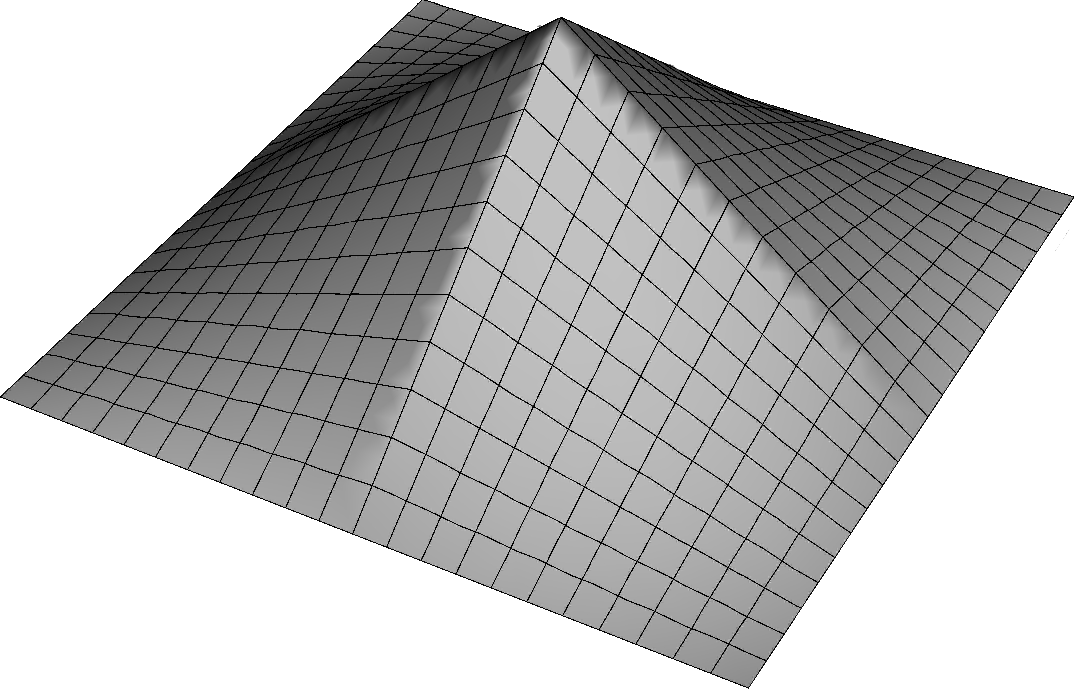
\includegraphics[width=0.5\textwidth]{./figuras-tikz/Cap11-Theta.pdf}\\[5pt]
    {\small Gráfica de $\Theta$}
%    % \caption{}\label{fig:11.1}
  \end{figure}

Esta función es continua y tiene las siguientes propiedades.

\begin{lemma}
  \label{piramides}

  \begin{enumerate}
  \item[(a)] $\sop(\Theta_{\delta })=[-\delta ,\delta ]^{n}$.

  \item[(b)] $(\mathrm{T}_{\delta \xi }\Theta_{\delta })(x)=\left(
      \mathrm{T}_{\xi }\Theta \right) (\frac{x}{\delta })$\quad para
    cualesquiera $x\in \mathbb{R}^{n}$, $\xi \in \mathbb{R}^{n}$.

  \item[(c)] $\sum_{m\in \mathbb{Z}^{n}}\mathrm{T}_{\delta m}\Theta
   _{\delta }=1$,\quad donde $\mathbb{Z}^{n}$ denota a los puntos de
    $\mathbb{R}^{n}$ de coordenadas enteras.
  \end{enumerate}
\end{lemma}

\begin{proof}
  La afirmación \emph{(a)} es inmediata, pues sop$(\Theta
  )=[-1,1]^{n}$. La afirmación \emph{(b)} también es clara, ya
  que\
  \begin{equation*}
    (\mathrm{T}_{\delta \xi }\Theta_{\delta })(x)=\Theta_{\delta }(x-\delta
    \xi )=\Theta (\tfrac{x}{\delta }-\xi )=(\mathrm{T}_{\xi }\Theta )(\tfrac{x}{\delta }).
  \end{equation*}
  Para probar \emph{(c)} observa primero que, si $t\in [j-1,j]$
  con $j\in \mathbb{Z}$, entonces
  \begin{equation*}
    \sum_{k\in \mathbb{Z}}\theta (t-k)=\theta (t-(j-1))+\theta
    (t-j)=1-(t-j+1)+1-(j-t)=1.
  \end{equation*}
\begin{figure}[H]
  \centering
  \begin{tikzpicture}[scale=1.2]
  \pgfmathsetmacro{\xO}{1}
  \draw[very thick] (-3,0)--(3,0);
  \draw[very thin] (0,0)--(0,1.2);

  \draw[very thick] (-3,0)--(-2,1)--(-1,0)--(0,1)--(1,0)--(2,1)--(3,0);
  \draw[very thick](-3,1)--(-2,0)--(-1,1)--(0,0) --(1,1)--(2,0)--(3,1);
  \draw[very thin] (-0.06,1)--(0,1);
%  \draw (0,1.1) node[left] {$1$};

%\foreach \x in {-3,-2,-1,0,1,2,3}{
%  \draw[very thin] (\x,0)--(\x,-.05) node[below] {$\x$};               
%};
\draw[thick] (1.7,0) circle(.7pt);
\draw (1.7,-0.05) node[below] {$t$};
\end{tikzpicture}

  % \caption{}\label{fig:11.4}
\end{figure}
Por tanto,
  \begin{equation*}
    \sum_{k\in \mathbb{Z}}\mathrm{T}_{k}\theta =1.
  \end{equation*}
  En consecuencia, si $m=(m_{1},\dots,m_{n})\in \mathbb{Z}^{n}$, dado
  que
  \begin{equation*}
    \left( \mathrm{T}_{m}\Theta \right) (x_{1},\dots,x_{n})=\left( \mathrm{T}_{m_{1}}\theta \right) (x_{1})\cdots \left( \mathrm{T}_{m_{n}}\theta \right)
    (x_{n}),
  \end{equation*}
  se cumple que
  \begin{equation*}
    \sum_{m\in \mathbb{Z}^{n}}\left( \mathrm{T}_{m}\Theta \right)
    (x_{1},\dots,x_{n})=\biggl( \sum_{m_{1}\in \mathbb{Z}}\left( \mathrm{T}_{m_{1}}\theta \right) (x_{1})\biggr) \cdots \biggl( \sum_{m_{n}\in \mathbb{Z}}\left( \mathrm{T}_{m_{n}}\theta \right) (x_{n})\biggr) =1,
  \end{equation*}
  es decir,
  \begin{equation*}
    \sum_{m\in \mathbb{Z}^{n}}\mathrm{T}_{m}\Theta =1.
  \end{equation*}
  De esta identidad y la identidad \emph{(b) }se sigue inmediatamente
  \emph{(c).}
\end{proof}

Observa que, si $f\in \mathcal{C}_{c}^{0}(\mathbb{R}^{n})$, entonces
$f(\delta m)\neq 0$ únicamente para un número finito de $m\in
\mathbb{Z}^{n}$. Por tanto, la función
\begin{equation*}
  \sum_{m\in \mathbb{Z}^{n}}f(\delta m)\mathrm{T}_{\delta m}\Theta_{\delta }
\end{equation*}
es una suma finita de funciones continuas con soporte compacto y, en
consecuencia, pertenece a $\mathcal{C}_{c}^{0}(\mathbb{R}^{n})$.

\begin{lemma}
  \label{lemhaar2}Para cada $f\in
  \mathcal{C}_{c}^{0}(\mathbb{R}^{n})$,
  \begin{equation*}
    \lim_{\delta \rightarrow 0}\left\Vert f-\sum_{m\in \mathbb{Z}^{n}}f(\delta
      m)\mathrm{T}_{\delta m}\Theta_{\delta }\right\Vert_{\infty }=0.
  \end{equation*}
\end{lemma}

\begin{proof}
  Sea $\varepsilon >0$. Como $f$ tiene soporte compacto, $f$ es
  uniformemente continua en $\mathbb{R}^{n}$
  [Ejercicio~\ref{sopcompesunifcont}]. Por tanto, existe $\rho >0$ tal
  que
  \begin{equation*}
    \left\vert f(x)-f(y)\right\vert <\varepsilon \text{\qquad si }\left\Vert
      x-y\right\Vert <\rho .
  \end{equation*}
  Sea $\delta <\frac{\rho }{\sqrt{n}}$. Usando la afirmación
  \emph{(c)} del Lema~\ref{piramides}, para cada $x\in \mathbb{R}^{n}$
  obtenemos
  \begin{align}
    f(x)-\sum_{m\in \mathbb{Z}^{n}}f(\delta m)(\mathrm{T}_{\delta m}\Theta
   _{\delta })(x) &=\sum_{m\in \mathbb{Z}^{n}}\left( f(x)-f(\delta m)\right) (\mathrm{T}_{\delta m}\Theta_{\delta })(x)  \notag \\
    &=\sum_{m\in S(x)}\left( f(x)-f(\delta m)\right) (\mathrm{T}_{\delta
      m}\Theta_{\delta })(x),  \label{suma}
  \end{align}
  donde $S(x):=\left\{m\in \mathbb{Z}^{n}:x\in\sop(\mathrm{T}_{\delta
    m}\Theta_{\delta })\right\}$. Nota que $S(x)$ es un conjunto
  finito. Ahora bien, como
  \begin{equation*}
    \sop(\mathrm{T}_{\delta m}\Theta_{\delta })=\left\{x\in \mathbb{R}^{n}:x-\delta m\in [-\delta ,\delta ]^{n}\right\},
  \end{equation*}
  se tiene que
  \begin{equation*}
    \left\Vert x-\delta m\right\Vert \leq \sqrt{n}\delta <\rho \text{\qquad }\forall m\in S(x).
  \end{equation*}
  Aplicando la desigualdad del triángulo a (\ref{suma}) concluimos
  que
  \begin{align*}
    \left\vert f(x)-\sum_{m\in \mathbb{Z}^{n}}f(\delta m)(\mathrm{T}_{\delta
        m}\Theta_{\delta })(x)\right\vert &\leq \sum_{m\in S(x)}\left\vert
      f(x)-f(\delta m)\right\vert (\mathrm{T}_{\delta m}\Theta_{\delta })(x) \\
    &<\varepsilon \sum_{m\in S(x)}(\mathrm{T}_{\delta m}\Theta_{\delta
    })(x)\leq \varepsilon \text{\qquad si \ }\delta <\frac{\rho }{\sqrt{n}}.
  \end{align*}
  En consecuencia,
  \begin{equation*}
    \left\Vert f-\sum_{m\in \mathbb{Z}^{n}}f(\delta m)\mathrm{T}_{\delta
        m}\Theta_{\delta }\right\Vert_{\infty }\leq \varepsilon \text{\qquad si \ }\delta <\frac{\rho }{\sqrt{n}}.
  \end{equation*}
  Esto concluye la demostración.
\end{proof}

Finalmente, calcularemos $J(\Theta_{2^{-k}})$ en términos de
$J(\Theta )$.

\begin{lemma}
  \label{lemhaar3}Sea
  $J\colon \mathcal{C}_{c}^{0}(\mathbb{R}^{n})\rightarrow \mathbb{R}$ una
  función lineal e invariante bajo traslaciones. Entonces, para
  cada $\delta >0$, se cumple que
  \begin{equation*}
    2^{n}J(\Theta_{\delta })=J(\Theta_{2\delta }).
  \end{equation*}
  En consecuencia,
  \begin{equation*}
    2^{nk}J(\Theta_{2^{-k}})=J(\Theta )\qquad \forall k\in \mathbb{N}\text{.}
  \end{equation*}
\end{lemma}

\begin{proof}
  Un cálculo directo, que proponemos como ejercicio
  [Ejercicio~\ref{dilatacion}] y aquí ilustramos con una figura,
  muestra que
  \begin{equation*}
    \tfrac{1}{2}\,\theta (2t+1)+\theta (2t)+\tfrac{1}{2}\,\theta (2t-1)=\theta
    (t)\qquad \forall t\in \mathbb{R}\text{.}
  \end{equation*}
\begin{figure}[H]
  \centering
  \begin{tikzpicture}[scale=1.7]
  \pgfmathsetmacro{\xO}{1}
  \draw[very thin] (-1.5,0)--(1.5,0);
  \draw[very thin] (0,0)--(0,1);

  \draw[very thick] (-1,0)--(-.5,.5)--(0,0)--(.5,.5)--(1,0);
  \draw[very thick] (-.5,0)--(0,1)--(.5,0);
  \draw[very thick] (-1.5,0)--(1.5,0);

  \draw[very thin] (0,1)--(-0.05,1) node[left] {\scriptsize $1$};

\foreach \x in {-1,-0.5,0,0.5,1}{
  \draw[very thin] (\x,0)--(\x,-.05) node[below] {\scriptsize $\x$};
};
\end{tikzpicture}
\qquad 
  \begin{tikzpicture}[scale=1.7]
  \pgfmathsetmacro{\xO}{1}
  \draw[very thin] (-1.5,0)--(1.5,0);
  \draw[very thin] (0,0)--(0,1);

  \draw[very thick] (-1.5,0)--(-1,0)--(0,1)--(1,0)--(1.5,0);
  \draw (-.5,.5)--(0,0)--(.5,.5);
  \draw (-.5,0)--(0,1)--(.5,0);
  \draw (-1.5,0)--(1.5,0);

\foreach \x in {0.5,1}{
  \draw[very thin] (-0.05,\x)--(0,\x);% node[left] {$\x$};
};
\foreach \x in {-1,-0.5,0,0.5,1}{
  \draw[very thin] (\x,0)--(\x,-.05) node[below] {\scriptsize $\x$};
};
\draw(-0.05,1) node[left] {\scriptsize $1$};
\end{tikzpicture}
 
  % \caption{}\label{fig:11.1}
\end{figure}
  Reemplazando $t$ por $\frac{t}{2\delta }$ en la identidad anterior
  obtenemos
{\abovedisplayskip=8pt
\belowdisplayskip=8pt
  \begin{align*}
    \theta_{2\delta }(t) =\theta \left( \tfrac{t}{2\delta }\right) &=\tfrac{1}{2}\,\theta \left( \tfrac{t+\delta }{\delta }\right) +\theta \left( \tfrac{t}{\delta }\right) +\tfrac{1}{2}\,\theta \left( \tfrac{t-\delta }{\delta }\right)
    \\
    &=\tfrac{1}{2}(\mathrm{T}_{-\delta }\theta_{\delta })(t)+\theta_{\delta
    }(t)+\tfrac{1}{2}(\mathrm{T}_{\delta }\theta_{\delta })(t)\qquad \forall
    t\in \mathbb{R}.
  \end{align*}
  Es decir,
  \begin{equation*}
    \theta_{2\delta }=\sum_{\nu \in \Gamma }\left( \tfrac{1}{2}\right)
   ^{\left\vert \nu \right\vert }\mathrm{T}_{\nu \delta }\theta_{\delta
    },\qquad \text{con \ }\Gamma :=\left\{-1,0,1\right\}.
  \end{equation*}
  Por tanto,
  \begin{align}
    \Theta_{2\delta }(x_{1},\dots,x_{n}) &=\theta_{2\delta }(x_{1})\cdots
    \theta_{2\delta }(x_{n})  \notag \\
    &=\sum_{\gamma \in \Gamma^{n}}c_{\gamma }(\mathrm{T}_{\gamma \delta
    }\Theta_{\delta })(x_{1},\dots,x_{n}),  \label{dil}
  \end{align}
  donde
  \begin{equation*}
    c_{\gamma }=\prod_{i=1}^{n}\left( \tfrac{1}{2}\right)^{\left\vert \gamma
       _{i}\right\vert }\text{\qquad con }\gamma =(\gamma_{1},\dots,\gamma_{n})\in
    \Gamma^{n}.
  \end{equation*}
  Observa que
  \begin{equation*}
    \sum_{\gamma \in \Gamma^{n}}c_{\gamma }=\left( \tfrac{1}{2}+1+\tfrac{1}{2}\right) \sum_{\gamma \in \Gamma^{n-1}}c_{\gamma }=\left( \tfrac{1}{2}+1+\tfrac{1}{2}\right)^{n}=2^{n}.
  \end{equation*}

  Como $J$ es lineal e invariante bajo traslaciones, aplicando $J$ a
  la identidad (\ref{dil}) concluimos que
  \begin{equation*}
    J(\Theta_{2\delta })=\sum_{\gamma \in \Gamma^{n}}c_{\gamma }J(\Theta
   _{\delta })=2^{n}J(\Theta_{\delta }).
  \end{equation*}
  Esta es la primera identidad del enunciado.

  Para probar la segunda aplicamos ésta $k$ veces, con $\delta
  =2^{-1},2^{-2},\dots,2^{-k}$ respectivamente, para obtener
  \begin{equation*}
    J(\Theta )=2^{n}J(\Theta_{2^{-1}})=2^{2n}J(\Theta_{2^{-2}})=\cdots
    =2^{kn}J(\Theta_{2^{-k}}).
  \end{equation*}
  Esto concluye la demostración.}%
\end{proof}

\begin{proof}[Demostración del Teorema~\ref{comphaar}.] Sea
$J\colon \mathcal{C}_{c}^{0}(\mathbb{R}^{n})\rightarrow \mathbb{R}$ una
medida de Haar y sea $c:=J(\Theta )$, donde $\Theta $ es la
función definida en (\ref{defTheta}). Denotemos por
$I\colon \mathcal{C}_{c}^{0}(\mathbb{R}^{n})\rightarrow \mathbb{R} $ a la
función
\begin{equation*}
  I(f):=\int_{\mathbb{R}^{n}}f.
\end{equation*}
Probaremos que
\begin{equation*}
  J(f)=cI(f)\text{\qquad }\forall f\in \mathcal{C}_{c}^{0}(\mathbb{R}^{n}).
\end{equation*}

Usando el Ejercicio~\ref{intprodtens}\ obtenemos
\begin{equation*}
  I(\Theta )=\biggl( \int_{\mathbb{R}}\theta \biggr)^{n}=1.
\end{equation*}
Aplicando el Lema~\ref{lemhaar3} tanto a $I$ como a $J$ concluimos que
\begin{equation*}
  J(\Theta_{2^{-k}})=2^{-kn}J(\Theta )=2^{-kn}cI(\Theta )=cI(\Theta
 _{2^{-k}}).
\end{equation*}
Sea $f\in \mathcal{C}_{c}^{0}(\mathbb{R}^{n})$. De los Lemas
\ref{lemhaar1} y~\ref{lemhaar2} se sigue que
\begin{align*}
  J(f) &=\lim_{k\rightarrow \infty }J\biggl( \sum_{m\in \mathbb{Z}^{n}}f(2^{-k}m)\mathrm{T}_{2^{-k}m}\Theta_{2^{-k}}\biggr) \\
  &=\lim_{k\rightarrow \infty }\sum_{m\in \mathbb{Z}^{n}}f(2^{-k}m)J(\Theta
 _{2^{-k}}) \\
  &=c\lim_{k\rightarrow \infty }\sum_{m\in \mathbb{Z}^{n}}f(2^{-k}m)I(\Theta
 _{2^{-k}}) \\
  &=c\lim_{k\rightarrow \infty }I\biggl( \sum_{m\in \mathbb{Z}^{n}}f(2^{-k}m)\mathrm{T}_{2^{-k}m}\Theta_{2^{-k}}\biggr) =cI(f).
\end{align*}
Esto concluye la demostración.
\end{proof}

\section{Invariancia bajo isometrías}

Sea $GL(n,\mathbb{R})$ el conjunto de todas las matrices invertibles
de $n\times n$ con coeficientes reales, es decir, de las matrices cuyo
determinante es distinto de cero. Si identificamos a una matriz $A$
con la transformación lineal $A\colon \mathbb{R}^{n}\rightarrow
\mathbb{R}^{n}$ definida por ella, de la manera usual, entonces
$GL(n,\mathbb{R})$ es el conjunto de isomorfismos lineales
$\mathcal{H}(\mathbb{R}^{n},\mathbb{R}^{n}) $ definido en la
Sección~\ref{isoBanach}.

$GL(n,\mathbb{R})$ con el producto de matrices (o la composición
de transformaciones lineales) es un grupo, que se llama \textbf{grupo
  lineal general}.  \index{grupo!lineal general@lineal general
  $GL(n,\mathbb{R})$}

Observa lo siguiente.

\begin{lemma}
  \label{newhaar}Si $J\colon \mathcal{C}_{c}^{0}(\mathbb{R}^{n})\rightarrow
  \mathbb{R}$ es una medida de Haar en $\mathbb{R}^{n}$\ y $A\in
  GL(n,\mathbb{R})$, entonces la función
  $J_{A}\colon \mathcal{C}_{c}^{0}(\mathbb{R}^{n})\rightarrow \mathbb{R}$
  dada por
  \begin{equation*}
    J_{A}(f):=J(f\circ A)
  \end{equation*}
  está bien definida y es una medida de Haar en $\mathbb{R}^{n}$.
\end{lemma}

\begin{proof}
  Sean $A\in GL(n,\mathbb{R})$ y $f\in
  \mathcal{C}_{c}^{0}(\mathbb{R}^{n})$. Puesto que\ sop$(f\circ
  A)=A^{-1}($sop$(f))$, se tiene que sop$(f\circ A)$\ es compacto (ver
  Proposición~\ref{compcont}). Así que $f\circ A\in
  \mathcal{C}_{c}^{0}(\mathbb{R}^{n})$. Esto prueba que $J_{A}$
  está bien definida.

  La linealidad y la monotonía de $J_{A}$ son consecuencia
  inmediata de las propiedades correspondientes de $J$. Probemos la
  invariancia bajo traslaciones.

  Sean $\xi \in \mathbb{R}^{n}$ y $f\in
  \mathcal{C}_{c}^{0}(\mathbb{R}^{n})$. Para todo $x\in
  \mathbb{R}^{n}$ se tiene que
  \begin{align*}
    \left( \left( \mathrm{T}_{\xi }f\right) \circ A\right) (x)=\left(
    \mathrm{T}_{\xi }f\right) (Ax)&=f(Ax-\xi )\\
 &=f(A(x-A^{-1}\xi ))=(\mathrm{T}_{A^{-1}\xi
   }(f\circ A))(x).
  \end{align*}
  Como $J$ es invariante bajo traslaciones concluimos que
  \begin{equation*}
    J_{A}(\mathrm{T}_{\xi }f)=J(\left( \mathrm{T}_{\xi }f\right) \circ A)=J(\mathrm{T}_{A^{-1}\xi }(f\circ A))=J(f\circ A)=J_{A}(f),
  \end{equation*}
  es decir, $J_{A}$ es invariante bajo traslaciones.
\end{proof}

Una matriz $A\in GL(n,\mathbb{R})$ se llama \textbf{ortogonal}
\index{matriz!ortogonal}si es una isometría, es decir, si
\begin{equation*}
  \left\Vert Ax\right\Vert =\left\Vert x\right\Vert 
  \text{\qquad }\forall x\in \mathbb{R}^{n}.
\end{equation*}
Si $A$ es una matriz ortogonal entonces $\det A=\pm 1$. El conjunto de
todas las matrices ortogonales de $n\times n$ es un subgrupo de
$GL(n,\mathbb{R})$, llamado el \textbf{grupo ortogonal,}
\index{grupo!ortogonal@ortogonal $O(n)$}que se denota por $O(n)$.

Usaremos el Teorema~\ref{comphaar} para probar que la integral es
invariante bajo isometrías.

\begin{theorem}[Invariancia bajo isometrías]
  \label{inviso}Para cualesquiera $A\in O(n)$, $\zeta \in
  \mathbb{R}^{n}$ y $f\in \mathcal{C}_{c}^{0}(\mathbb{R}^{n})$ se
  cumple que
  \begin{equation*}
    \int_{\mathbb{R}^{n}}f(Ax+\zeta )dx=\int_{\mathbb{R}^{n}}f(y)dy.
  \end{equation*}
\end{theorem}

{\abovedisplayskip=8pt
\belowdisplayskip=8pt
\begin{proof}
  Sean $I,I_{A}\colon \mathcal{C}_{c}^{0}(\mathbb{R}^{n})\rightarrow
  \mathbb{R}$ las funciones dadas por
  \begin{equation*}
    I(f):=\int_{\mathbb{R}^{n}}f,\text{\qquad }I_{A}(f):=I(f\circ A).
  \end{equation*}
  Ambas son medidas de Haar en $\mathbb{R}^{n}$ (ver
  Lema~\ref{newhaar}). Por el Teorema~\ref{comphaar}, existe una
  constante $c\geq 0$ tal que
  \begin{equation}
    I_{A}(f)=cI(f)\text{\qquad }\forall f\in \mathcal{C}_{c}^{0}(\mathbb{R}^{n}).
    \label{haarI}
  \end{equation}
  Probaremos que $c=1$. Para ello, considera la función
  \begin{equation*}
    f_{0}(x):=
      \begin{cases}
        1-\left\Vert x\right\Vert & \text{si $\left\Vert x\right\Vert \leq 1$,} \\ 
        0 & \text{si $\left\Vert x\right\Vert \geq 1$.}
      \end{cases}
  \end{equation*}
  \begin{figure}[H]
    \centering
    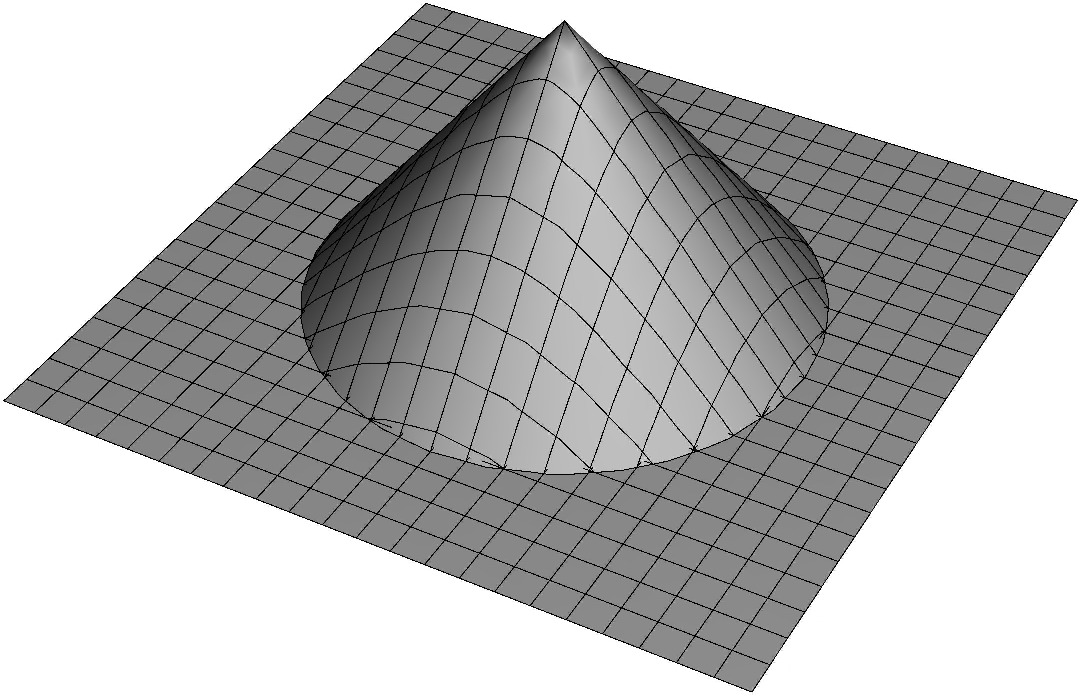
\includegraphics[width=0.5\textwidth]{./figuras-tikz/Cap11-cono.pdf}\\[5pt]
    {\small Gráfica de $f_0$}
%    % \caption{}\label{fig:11.1}
  \end{figure}
  \noindent
  Como $\left\Vert Ax\right\Vert =\left\Vert x\right\Vert $ para todo
  $x\in \mathbb{R}^{n}$, se tiene que $f_{0}=f_{0}\circ A$. En
  consecuencia,
  \begin{equation*}
    cI(f_{0})=I_{A}(f_{0})=I(f_{0}\circ A)=I(f_{0}),
  \end{equation*}
  y como $I(f_{0})\neq 0$ [Ejercicio~\ref{posi}] concluimos que $c=1$.
  Sustituyendo este valor en la identidad (\ref{haarI}) obtenemos
  \begin{equation*}
    \int_{\mathbb{R}^{n}}f\circ A=\int_{\mathbb{R}^{n}}f\text{\qquad }\forall
    f\in \mathcal{C}_{c}^{0}(\mathbb{R}^{n}).
  \end{equation*}
  Por último, usamos la invariancia de la integral bajo
  traslaciones para concluir que
  \begin{equation*}
    \int_{\mathbb{R}^{n}}(\mathrm{T}_{-\zeta }f)\circ A=\int_{\mathbb{R}^{n}}\mathrm{T}_{-\zeta }f=\int_{\mathbb{R}^{n}}f\text{\qquad }\forall f\in 
    \mathcal{C}_{c}^{0}(\mathbb{R}^{n}).
  \end{equation*}
  Ésta es la identidad deseada.
\end{proof}}%

Una consecuencia sencilla pero importante del Teorema~\ref{inviso} es
que la integral no depende del orden de las variables.

\begin{corollary}
  \label{orden}Para cualquier permutación $(i_{1},\dots,i_{n})$ de
  $(1,\dots,n) $ se cumple que
  \begin{equation*}
    \int_{\mathbb{R}^{n}}f(x_{1},x_{2},\dots,x_{n})dx_{1}\cdots dx_{n}=\int_{\mathbb{R}^{n}}f(x_{1},x_{2},\dots,x_{n})dx_{i_{1}}\cdots dx_{i_{n}}.
  \end{equation*}
\end{corollary}

\begin{proof}
  Sea $A$ la matriz que permuta coordenadas como sigue:
  \begin{equation*}
    A(x_{1},x_{2},\dots,x_{n})=(y_{1},y_{2},\dots,y_{n}),\text{\qquad donde \ }y_{k}:=x_{j}\text{ si }i_{j}=k.
  \end{equation*}
  Claramente, $\left\Vert Ax\right\Vert =\left\Vert x\right\Vert $
  para todo $x\in \mathbb{R}^{n}$, por tanto $A\in O(n)$. Aplicando el
  Teorema~\ref{inviso}\ obtenemos
  \begin{align*}
    \int_{\mathbb{R}^{n}}f(x_{1},x_{2},\dots,x_{n})dx_{1}\cdots dx_{n} &=\int_{\mathbb{R}^{n}}(f\circ A)(x_{1},x_{2},\dots,x_{n})dx_{1}\cdots dx_{n} \\
    &=\int_{\mathbb{R}^{n}}f(y_{1},y_{2},\dots,y_{n})dy_{i_{1}}\cdots dy_{i_{n}},
  \end{align*}
  como afirma el enunciado.
\end{proof}

El Teorema~\ref{inviso} se extiende como sigue.

\begin{theorem}
  \label{cvlin}Para cualesquiera $A\in GL(n,\mathbb{R})$, $\zeta \in
  \mathbb{R}^{n}$ y $f\in \mathcal{C}_{c}^{0}(\mathbb{R}^{n})$ se
  cumple que
  \begin{equation*}
    \int_{\mathbb{R}^{n}}f(Ax+\zeta )\left\vert \det A\right\vert dx=\int_{\mathbb{R}^{n}}f(y)dy.
  \end{equation*}
\end{theorem}

Para demostrar este teorema usaremos el siguiente caso particular de
él.

\begin{lemma}
  \label{diag}Si $A$ es una matriz diagonal de $n\times n$ tal que
  $\det A\neq 0$, entonces para toda $f\in
  \mathcal{C}_{c}^{0}(\mathbb{R}^{n})$ se cumple que
  \begin{equation*}
    \int_{\mathbb{R}^{n}}f(Ax)\left\vert \det A\right\vert dx=\int_{\mathbb{R}^{n}}f(y)dy.
  \end{equation*}
\end{lemma}

{\abovedisplayskip=8pt
\belowdisplayskip=8pt
\begin{proof}
  Sea
  \begin{equation*}
    A=
      \begin{pmatrix}
        \lambda_{1} & \cdots & 0 \\ 
        \vdots & \ddots & \vdots \\ 
        0 & \cdots & \lambda_{n}
      \end{pmatrix}.
  \end{equation*}
  tal que $\det A=\lambda_{1}\cdots \lambda_{n}\neq 0$. Considera la
  medida de Haar $I_{A}\colon \mathcal{C}_{c}^{0}(\mathbb{R}^{n})\rightarrow
  \mathbb{R}$ dada por
  \begin{equation*}
    I_{A}(f):=\int_{\mathbb{R}^{n}}f\circ A
  \end{equation*}
  (ver Lema~\ref{newhaar}). Por el Teorema~\ref{comphaar}\ existe
  $c\geq 0$ tal que
  \begin{equation}
    I_{A}(f)=c\int_{\mathbb{R}^{n}}f\text{\qquad }\forall f\in \mathcal{C}_{c}^{0}(\mathbb{R}^{n}).  \label{diaghaar}
  \end{equation}
  Para determinar $c$ basta calcular el valor de $I_{A}$ en la
  función $\Theta $ definida en (\ref{defTheta}). Nota que, para
  $\lambda\neq0$,
  \begin{equation*}
    \theta (\lambda t)=
      \begin{cases}
        1-\left\vert \lambda t\right\vert & \text{si $\left\vert t\right\vert \leq 
        \frac{1}{\left\vert \lambda \right\vert }$,} \\ 
        0 & \text{si $\left\vert t\right\vert \geq \frac{1}{\left\vert \lambda
          \right\vert }$.}
      \end{cases}
  \end{equation*}
  Por tanto,
  \begin{equation*}
    \int_{\mathbb{R}}\theta (\lambda t)dt=\frac{1}{\left\vert \lambda
      \right\vert }
  \end{equation*}
  y, en consecuencia,
  \begin{align*}
    \int_{\mathbb{R}^{n}}\Theta \circ A &=\int_{\mathbb{R}^{n}}\theta (\lambda
   _{1}x_{1})\cdots \theta (\lambda_{n}x_{n})dx_{1}\cdots dx_{n} \\
    &=\frac{1}{\left\vert \lambda_{1}\right\vert }\cdots \frac{1}{\left\vert
        \lambda_{n}\right\vert }=\frac{1}{\left\vert \det A\right\vert }.
  \end{align*}
  Como $\int_{\mathbb{R}^{n}}\Theta =1$ concluimos que
  \begin{equation*}
    \frac{1}{\left\vert \det A\right\vert }=I_{A}(\Theta )=c\int_{\mathbb{R}^{n}}\Theta =c.
  \end{equation*}
  Sustituyendo este valor en la identidad (\ref{diaghaar}) obtenemos
  \begin{equation*}
    \int_{\mathbb{R}^{n}}f\circ A=\frac{1}{\left\vert \det A\right\vert }\int_{\mathbb{R}^{n}}f\text{\qquad }\forall f\in \mathcal{C}_{c}^{0}(\mathbb{R}^{n}),
  \end{equation*}
  como afirma el enunciado.
\end{proof}}%

Usaremos el siguiente resultado de algebra lineal\footnote{Consulta,
  por ejemplo,~\cite{Friedberg} (Theorem 6.27).} para probar el Teorema~\ref{cvlin}.

\begin{theorem}[Descomposición en valores singulares]
  \label{svd}Sea $A$ una matriz de $n\times n$ con coeficientes
  reales.  Entonces existen $U_{1},U_{2}\in O(n)$ y una matriz
  diagonal $D$ con coeficientes no negativos tales que
   $A=U_{1}DU_{2}$.
  % \begin{equation*}
  %   A=U_{1}DU_{2}.
  % \end{equation*}
\end{theorem}

Proponemos la demostración de este resultado como ejercicio
[Ejercicio~\ref{ejersvd}].

\begin{proof}[Demostración del Teorema~\ref{cvlin}.] Sean $A\in
GL(n,\mathbb{R})$, $\zeta \in \mathbb{R}^{n}$ y $f\in
\mathcal{C}_{c}^{0}(\mathbb{R}^{n})$. Por el Teorema~\ref{svd},
existen $U_{1},U_{2}\in O(n)$ y una matriz diagonal $D$ tales que
\begin{equation*}
  A=U_{1}DU_{2}.
\end{equation*}
En particular, $\left\vert \det D\right\vert =\left\vert \det
  A\right\vert \neq 0$. Usando el Teorema~\ref{inviso}, el Lema
\ref{diag}\ y la invariancia de la integral bajo traslaciones,
obtenemos
\begin{align*}
  \int_{\mathbb{R}^{n}}f(x)dx &=\int_{\mathbb{R}^{n}}f(U_{1}x)dx=\int_{\mathbb{R}^{n}}f(U_{1}Dx)\left\vert \det D\right\vert dx \\
  &=\int_{\mathbb{R}^{n}}f(U_{1}DU_{2}x)\left\vert \det D\right\vert dx=\int_{\mathbb{R}^{n}}f(Ax)\left\vert \det A\right\vert dx \\
  &=\int_{\mathbb{R}^{n}}f(Ax+\zeta )\left\vert \det A\right\vert dx,
\end{align*}
como afirma el enunciado.
\end{proof}

\section{El teorema de cambio de variable}

Ahora nuestro objetivo es extender el Teorema~\ref{cvlin},\
reemplazando a la transformación $x\mapsto Ax+\zeta \ $por una
función $\varphi $ que localmente se parece a ella. Empezaremos
precisando lo que esto significa.

A lo largo de esta sección $\Omega $ denotará a un subconjunto
abierto de $\mathbb{R}^{n}$.

\begin{definition}
  Sea $f\in \mathcal{C}^{0}(\Omega )$. El \textbf{soporte de} $f$
  \index{soporte}es la cerradura en $\mathbb{R}^{n}$ del conjunto
  $\left\{x\in \Omega :f(x)\neq 0\right\}$. Lo denotamos $\sop(f)$.
\end{definition}

Nota que el soporte de una función $f\in \mathcal{C}^{0}(\Omega )$
no necesariamente está contenido en $\Omega $. Por ejemplo, si
$f(x)=1$ para todo $x\in \Omega $ entonces sop$(f)=\overline{\Omega
}$, que no está contenido en $\Omega $ si $\Omega \neq
\mathbb{R}^{n}$.

Definimos
\begin{equation*}
  \mathcal{C}_{c}^{0}(\Omega ):=\left\{f\in \mathcal{C}^{0}(\Omega ) :
    \sop(f)\text{ es compacto y }\sop(f)\subset \Omega \right\}.
\end{equation*}
Nota que $\mathcal{C}_{c}^{0}(\Omega )$ es un subespacio vectorial de
$\mathcal{C}^{0}(\Omega )$ (ver Ejercicio~\ref{sop}).
\index{espacio!C subc0Omega@$\mathcal{C}_{c}^{0}(\Omega ) \vspaceindex$}
Si $\Omega =\mathbb{R}^{n}$
este espacio coincide con el de la Definición~\ref{defsop}.

Dada una función $f\colon \Omega \rightarrow \mathbb{R}$, denotamos por
$\bar{f}\colon \mathbb{R}^{n}\rightarrow \mathbb{R}$ a la función
\begin{equation*}
  \bar{f}(x):=
    \begin{cases}
      f(x) & \text{si $x\in \Omega$,} \\ 
      0 & \text{si $x\in \mathbb{R}^{n}\smallsetminus \Omega$.}
    \end{cases}
\end{equation*}
Es sencillo comprobar que, si $f\in \mathcal{C}_{c}^{0}(\Omega )$,
entonces $\bar{f}$ es continua en todo $\mathbb{R}^{n}$ y pertenece a
$\mathcal{C}_{c}^{0}(\mathbb{R}^{n})$ [Ejercicio~\ref{ext}].

\begin{definition}
  Si $f\in \mathcal{C}_{c}^{0}(\Omega )$ definimos \textbf{la integral
    de} $f$ \textbf{en} $\Omega $
  \index{integral!de una función continua}como
  \begin{equation*}
    \int_{\Omega }f:=\int_{\mathbb{R}^{n}}\bar{f}.
  \end{equation*}
\end{definition}

\begin{definition}
  Sean $\Omega $ y $\Omega^{\prime }$ subconjuntos abiertos de
  $\mathbb{R}^{n}$. Una función $\varphi \colon \Omega \rightarrow
  \Omega^{\prime }$ es un \textbf{difeomorfismo de clase}
  $\mathcal{C}^{1}$ \index{difeomorfismo!de clase C1@de clase
    $\mathcal{C}^{1}$}si $\varphi $ es de clase $\mathcal{C}^{1}$ en
  $\Omega $, $\varphi $ es biyectiva y su inverso $\varphi
 ^{-1}\colon \Omega^{\prime }\rightarrow \Omega $ es de clase
  $\mathcal{C}^{1}$ en $\Omega^{\prime }$.
\end{definition}

Si $\varphi $ es un difeomorfismo de clase $\mathcal{C}^{1}$, la regla
de la cadena asegura que
\begin{equation*}
  (\varphi^{-1})^{\prime }(\varphi (\xi ))\circ \varphi^{\prime }(\xi )=\id\text{\qquad y\qquad }\varphi^{\prime }(\xi )\circ (\varphi^{-1})^{\prime
  }(\varphi (\xi ))=\id\text{\qquad }\forall \xi \in \Omega ,
\end{equation*}
donde $\id\colon \mathbb{R}^{n}\rightarrow \mathbb{R}^{n}$ es la
identidad. Por tanto, $\varphi^{\prime }(\xi )\in GL(n,\mathbb{R})$
para todo $\xi \in \Omega $. En una vecindad pequeña de $\xi $, la
función $\varphi $ es muy cercana a la función
\begin{equation*}
  \alpha_{\xi }(x):=\varphi (\xi )+\varphi^{\prime }(\xi )[x-\xi]=\varphi
 ^{\prime }(\xi )x+\left[ \varphi (\xi )-\varphi^{\prime }(\xi )\xi \right] ,
\end{equation*}
para la cual vale el Teorema~\ref{cvlin}. Probaremos la siguiente
extensión de ese resultado.

\begin{theorem}[de cambio de variable]
  \label{cv}Sean $\Omega $ y $\Omega^{\prime }$ subconjuntos abiertos
  de $\mathbb{R}^{n}$, $\varphi \colon \Omega \rightarrow \Omega^{\prime }$
  un difeomorfismo de clase $\mathcal{C}^{1}$ y $f\in
  \mathcal{C}_{c}^{0}(\Omega^{\prime })$. Entonces $(f\circ \varphi
  )\left\vert \det \varphi^{\prime }\right\vert \in
  \mathcal{C}_{c}^{0}(\Omega )$ y
  \begin{equation*}
    \int_{\Omega }f(\varphi (x))\left\vert \det \varphi^{\prime }(x)\right\vert
    dx=\int_{\Omega^{\prime }}f(y)dy.
  \end{equation*}
\end{theorem}

La idea de la demostración es aproximar localmente a $\varphi $
por la función $\alpha_{\xi }$ y aplicar el Teorema
\ref{cvlin}. Dedicaremos el resto de esta sección a la
demostración de este resultado. Usaremos el siguiente lema.

\begin{lemma}
  \label{omega}Sean $K=(K,d_{K})$ un espacio métrico compacto,
  $X=(X,d_{X}) $ un espacio métrico y $\varphi \colon K\rightarrow X$
  una función continua. Entonces existe una función no
  decreciente $\omega \colon [0,\infty )\rightarrow [0,\infty )$ tal
  que $\lim_{t\rightarrow 0^{+}}\omega (t)=0$ y
  \begin{equation*}
    d_{X}(\varphi (x),\varphi (y))\leq \omega (d_{K}(x,y))\text{\qquad }\forall
    x,y\in K.
  \end{equation*}
\end{lemma}

\begin{proof}
  Para cada $t\in [0,\infty )$ definimos
  \begin{equation}
    \omega (t):=\sup \left\{d_{X}(\varphi (x),\varphi (y)):x,y\in K,\text{ }d_{K}(x,y)\leq t\right\}.  \label{mod}
  \end{equation}
  Como la función $h\colon K\times K\rightarrow \mathbb{R}$ dada por
  $h(x,y):=d_{X}(\varphi (x),\varphi (y))$ es continua (ver
  Ejercicio~\ref{distcont}) y $K\times K$ es compacto (ver
  Ejercicio~\ref{prodcomp}), se tiene que $h$ es acotada. Por tanto,
  $\omega (t)\in [0,\infty )$ para todo $t\in [0,\infty )$.
  Claramente, $\omega (t)\leq \omega (s)$ si $t\leq s$. Además, como
  $\varphi $ es uniformemente continua en $K$, dada $\varepsilon >0$,
  existe $\delta >0$ tal que
  \begin{equation*}
    d_{X}(\varphi (x),\varphi (y))<\varepsilon \text{\qquad si \ }d_{K}(x,y)<\delta .
  \end{equation*}
  En consecuencia, $\omega (t)\in [0,\varepsilon ]$ si $t\in
  [0,\delta )$, es decir, $\lim_{t\rightarrow 0^{+}}\omega
  (t)=0$. Por último, si $x,y\in K$ y $t:=d_{K}(x,y)$, de la
  definición de $\omega $ se sigue que
  \begin{equation*}
    d_{X}(\varphi (x),\varphi (y))\leq \omega (t)=\omega (d_{K}(x,y)).
  \end{equation*}
  Esto concluye la demostración.
\end{proof}

{\abovedisplayskip=7pt
\belowdisplayskip=7pt
La función $\omega $ definida en (\ref{mod}) es la función
óptima para la cual se cumple la desigualdad del lema. Se le llama
el \emph{módulo de continuidad uniforme} de $\varphi $.

Para $x=(x_{1},\dots,x_{n})\in \mathbb{R}^{n}$ denotamos por
\begin{align*}
  \left\Vert x\right\Vert_{\infty } &:=\max_{i=1,\dots,n}\left\vert
    x_{i}\right\vert , \\
  Q(x,\delta ) &:=\left\{y\in \mathbb{R}^{n}:\left\Vert y-x\right\Vert_{\infty
  }\leq \delta \right\}.
\end{align*}
Recuerda que $\left\Vert \cdot \right\Vert_{\infty }$ es una norma en
$\mathbb{R}^{n}$ que cumple
\begin{equation}
  \tfrac{1}{\sqrt{n}}\left\Vert x\right\Vert \leq \left\Vert x\right\Vert
 _{\infty }\leq \left\Vert x\right\Vert \text{\qquad }\forall x\in \mathbb{R}^{n}  \label{compnormas}
\end{equation}
(ver Ejercicio~\ref{ejRnormequiv}). A continuación introduciremos
los conjuntos y las constantes que usaremos en los siguientes lemas y
en la demostración del Teorema~\ref{cv}.

\begin{notation}
  Sean $\Omega $ y $\Omega^{\prime }$ abiertos en $\mathbb{R}^{n}$,
  $\varphi \colon \Omega \rightarrow \Omega^{\prime }$ un difeomorfismo de
  clase $\mathcal{C}^{1}$ y $f\in \mathcal{C}_{c}^{0}(\Omega^{\prime
  })$. Definimos
  \begin{equation*}
    K^{\prime }:=\sop(f)\text{\qquad y\qquad }K:=\varphi^{-1}(K^{\prime
    }).
  \end{equation*}
  Como $K$ y $K^{\prime }$ son subconjuntos compactos de $\Omega $ y
  $\Omega^{\prime }$ respectivamente, las distancias de $K$ a
  $\mathbb{R}^{n}\smallsetminus \Omega $ y de $K^{\prime }$ a
  $\mathbb{R}^{n}\smallsetminus \Omega^{\prime }$ son positivas
  \emph{(ver Ejercicio~\ref{dist>0})}. Por tanto, existe $\delta
 _{1}>0$ tal que
  \begin{alignat*}{2}
    Q(\xi ,\delta_{1}) &\subset \Omega &\qquad&\forall \xi \in K, \\
    Q(\zeta ,\delta_{1}) &\subset \Omega^{\prime }&&\forall \zeta
    \in K^{\prime }.
  \end{alignat*}

  Sean
  \begin{equation*}
    K_{1}:=\bigcup_{\xi \in K}Q(\xi ,\delta_{1})\text{\qquad y\qquad }K_{1}^{\prime }:=\bigcup_{\zeta \in K^{\prime }}Q(\zeta ,\delta_{1}).
  \end{equation*}
  \begin{figure}[H]
    \centering
    \begin{tikzpicture}[scale=0.75]
  \pgfmathsetmacro{\izq}{0}
  \pgfmathsetmacro{\verizq}{0}
  \pgfmathsetmacro{\verizqK}{0.1}
  \pgfmathsetmacro{\der}{6}
  \pgfmathsetmacro{\rectizqx}{.3}
  \pgfmathsetmacro{\rectizqy}{.8}
  \pgfmathsetmacro{\rectderx}{6.9}
  \pgfmathsetmacro{\rectdery}{0.3}
% Para la Omega 
  \draw[fill=gray!25] plot[smooth cycle, tension=.9]
  coordinates{(\izq-1,\verizq+0.7) (\izq+0.4,\verizq-0.9) (\izq+2,\verizq+.45) (\izq+0.6,\verizq+1.8)};
% Para la Omega' 
  \draw[fill=gray!25] plot[smooth cycle, tension=.9]
  coordinates{(\der-1.5,-1) (\der+0, -1) (\der+1.5,-0.65) (\der+2,1.45) (\der+0.3,1.6) (\der-1.3,1.3)};
% Para la K 
  \draw[very thin,fill=gray!50] plot[smooth cycle, tension=.9]
  coordinates{(\izq-0.1,\verizqK+0.05) (\izq+0.5,\verizqK+0.1) (\izq+1.1,\verizqK-0.05) (\izq+.8,\verizqK+.75) (\izq+0,\verizqK+0.8)};
% Para la K' 
  \draw[very thin,fill=gray!50] plot[smooth cycle, tension=.9]
  coordinates{(\der-0.6,0.05) (\der+.15,-0.05) (\der+0.5, 0.2)
    (\der+1.1,-0.05) (\der+1,.55) (\der-0.5,0.8)};
% Los cuadrados
  \draw[very thin] (\rectizqx+0,\rectizqy+0) rectangle (\rectizqx+.4,\rectizqy+.4);
  \draw[very thin] (\rectderx+0,\rectdery+0) rectangle (\rectderx+.4,\rectdery+.4);
% La flecha
  \draw[-latex'] (1,.7) .. controls (2.2,1.2) and (4.3,1.2) .. 
  node[above] {$\varphi$} (5.2,.7);
% Las etiquetas
  \node at (\izq+0.35,0.45) {$K$};
  \node at (\der-0.1,0.3) {$K'$};
  \node at (\izq+1,-0.45) {$\Omega$};
  \node at (\der+1.1,-0.6) {$\Omega'$};
\end{tikzpicture}

    % \caption{}\label{fig:11.7}
  \end{figure}
  \noindent
  $K_{1}$ y $K_{1}^{\prime }$ son subconjuntos compactos de $\Omega $
  y $\Omega^{\prime }$ respectivamente \emph{(ver
    Ejercicio~\ref{unibolas})}.  Por tanto, como $\varphi^{\prime }$
  es continua en $K_{1}$ y $(\varphi^{-1})^{\prime }$ es continua en
  $K_{1}^{\prime }$, existe $M\in \mathbb{R}$ tal que
  \begin{equation*}
    \sup_{x\in K_{1}}\left\Vert \varphi^{\prime }(x)\right\Vert_{\mathcal{L}(\mathbb{R}^{n},\mathbb{R}^{n})}\leq M\text{\qquad y\qquad }\sup_{y\in
      K_{1}^{\prime }}\left\Vert (\varphi^{-1})^{\prime }(y)\right\Vert_{\mathcal{L}(\mathbb{R}^{n},\mathbb{R}^{n})}\leq M.
  \end{equation*}
  Definimos \ $c_{0}:=M\sqrt{n}$ \ y \ $\delta_{2}:=\min \left\{\delta
 _{1},\frac{\delta_{1}}{c_{0}}\right\}$.
\end{notation}

\begin{lemma}
  \label{cubos}Para cada $\delta \in (0,\delta_{1})$, $\xi \in K$ y
  $x\in \Omega $ se cumple lo siguiente:

  \begin{enumerate}
  \item[(a)] Si $\left\Vert \varphi (x)-\varphi (\xi )\right\Vert
   _{\infty }\leq \delta $, entonces $\left\Vert x-\xi \right\Vert
   _{\infty }\leq c_{0}\delta $.

  \item[(b)] Si $\left\Vert \varphi^{\prime }(\xi )\left[ x-\xi
      \right] \right\Vert_{\infty }\leq \delta $, entonces
    $\left\Vert x-\xi \right\Vert_{\infty }\leq c_{0}\delta $.
  \end{enumerate}
\end{lemma}

\begin{proof}
  \emph{(a):} \ Si
  $\left\Vert \varphi (x)-\varphi (\xi )\right\Vert _{\infty }\leq
  \delta $,
  entonces
  $y_{t}:=(1-t)\varphi (\xi )+t\varphi (x)\in Q(\varphi (\xi ),\delta
  )\subset K_{1}^{\prime }$
  para cada $t\in [0,1]$. Usando las desigualdades (\ref{compnormas})
  y el teorema del valor medio (ver Corolario~\ref{cortvm0}) obtenemos
  \begin{align*}
    \left\Vert x-\xi \right\Vert_{\infty } &\leq \left\Vert x-\xi \right\Vert
    =\left\Vert \varphi^{-1}(\varphi (x))-\varphi^{-1}(\varphi (\xi
      ))\right\Vert \\
    &\leq \sup_{t\in [0,1]}\left\Vert (\varphi^{-1})^{\prime
      }(y_{t})\right\Vert_{\mathcal{L}(\mathbb{R}^{n},\mathbb{R}^{n})}\left\Vert
      \varphi (x)-\varphi (\xi )\right\Vert \\
    &\leq M\sqrt{n}\left\Vert \varphi (x)-\varphi (\xi )\right\Vert_{\infty }
    \\
    &\leq c_{0}\delta .
  \end{align*}

  \emph{(b):} \ Si $\left\Vert \varphi^{\prime }(\xi )(x-\xi
    )\right\Vert_{\infty }\leq \delta $, usando las desigualdades
  (\ref{compnormas}) y (\ref{opernorm}) obtenemos
  \begin{align*}
    \left\Vert x-\xi \right\Vert_{\infty } &\leq \left\Vert x-\xi \right\Vert
    =\left\Vert (\varphi^{-1})^{\prime }(\varphi (\xi ))\left[ \varphi^{\prime
        }(\xi )\left[ x-\xi \right] \right] \right\Vert \\
    &\leq \left\Vert (\varphi^{-1})^{\prime }\left[ \varphi (\xi )\right]
    \right\Vert_{\mathcal{L}(\mathbb{R}^{n},\mathbb{R}^{n})}\left\Vert \varphi
     ^{\prime }(\xi )\left[ x-\xi \right] \right\Vert \\
    &\leq M\sqrt{n}\left\Vert \varphi^{\prime }(\xi )\left[ x-\xi \right]
    \right\Vert_{\infty } \\
    &\leq c_{0}\delta .
  \end{align*}
  Esto concluye la demostración.
\end{proof}}%

{\abovedisplayskip=8pt
\belowdisplayskip=8pt
Considera la función $\Theta_{\delta }\colon \mathbb{R}^{n}\rightarrow
\mathbb{R}$ definida en (\ref{Thetasubdelta}). Es sencillo comprobar
que
\begin{equation}
  \left\vert (\mathrm{T}_{\zeta }\Theta_{\delta })(x)-(\mathrm{T}_{\zeta
    }\Theta_{\delta })(y)\right\vert \leq \frac{n}{\delta }\left\Vert
    x-y\right\Vert_{\infty }\text{\qquad }\forall x,y\in \mathbb{R}^{n}.
  \label{TTheta}
\end{equation}
Proponemos esta desigualdad como ejercicio [Ejercicio~\ref{ThetaLip}].

\begin{lemma}
  \label{lemcv}Si $\zeta \in K^{\prime }$ y $\delta \in (0,\delta
 _{2})$, entonces
  \begin{equation*}
    \sop(\mathrm{T}_{\zeta }\Theta_{\delta })\subset K_{1}^{\prime
    }\qquad \text{y}\qquad \sop((\mathrm{T}_{\zeta }\Theta_{\delta
    })\circ \varphi )\subset K_{1}.
  \end{equation*}
  Además, existe una función $\omega \colon [0,\infty )\rightarrow
  [0,\infty )$ tal que $\lim_{t\rightarrow 0^{+}}\omega (t)=0$
  y
  \begin{equation*}
    \left\vert \int_{\Omega }(\mathrm{T}_{\zeta }\Theta_{\delta })(\varphi
      (x))\left\vert \det \varphi^{\prime }(x)\right\vert dx-\int_{\Omega
       ^{\prime }}(\mathrm{T}_{\zeta }\Theta_{\delta })(y)dy\right\vert \leq
    \omega (\delta )\delta^{n}
  \end{equation*}
para cualesquiera $\zeta \in K^{\prime }$, $\delta \in (0,\delta_{2})$. 
\end{lemma}}%

\begin{proof}
{\abovedisplayskip=8pt
\belowdisplayskip=8pt
  Sean $\zeta \in K^{\prime }$, $\xi :=\varphi^{-1}(\zeta )\in K$ y
  $\delta \in (0,\delta_{2})$. Denotemos por $\alpha_{\xi
  }\colon \mathbb{R}^{n}\rightarrow \mathbb{R}^{n}$ a la función $\alpha
 _{\xi }(x):=\varphi (\xi )+\varphi^{\prime }(\xi )\left[ x-\xi
  \right] $. Como sop$(\mathrm{T}_{\zeta }\Theta_{\delta })=Q(\zeta
  ,\delta )$ y $c_{0}\delta <\delta_{1}$, del Lema~\ref{cubos}\ se
  sigue que
  \begin{align}
    \sop((\mathrm{T}_{\zeta }\Theta_{\delta })\circ \varphi ) &\subset
    Q(\xi ,c_{0}\delta )\subset K_{1},  \label{sop1} \\
    \sop((\mathrm{T}_{\zeta }\Theta_{\delta })\circ \alpha_{\xi })
    &\subset Q(\xi ,c_{0}\delta )\subset K_{1}.  \label{sop2}
  \end{align}
  Por otra parte, como $\varphi^{\prime }(\xi )\in GL(n,\mathbb{R})$,
  aplicando el Teorema~\ref{cvlin} obtenemos
  \begin{equation*}
    \int_{\Omega }\left( \mathrm{T}_{\zeta }\Theta_{\delta }\right) (\alpha
   _{\xi }(x))\left\vert \det \varphi^{\prime }(\xi )\right\vert
    dx=\int_{\Omega^{\prime }}\left( \mathrm{T}_{\zeta }\Theta_{\delta
      }\right) (y)dy.
  \end{equation*}
  En consecuencia, bastará probar que existe una función
  $\omega \colon [0,\infty )\rightarrow [0,\infty )$ tal que
  $\lim_{t\rightarrow 0^{+}}\omega (t)=0$ y
  \begin{equation}
    \left\vert \int_{\Omega }(\mathrm{T}_{\zeta }\Theta_{\delta })(\varphi
      (x))\left\vert \det \varphi^{\prime }(x)\right\vert dx-\int_{\Omega }(\mathrm{T}_{\zeta }\Theta_{\delta })(\alpha_{\xi }(x))\left\vert \det
        \varphi^{\prime }(\xi )\right\vert dx\right\vert \leq \omega (\delta
    )\delta^{n}.  \label{zz}
  \end{equation}

  Sea $x\in Q(\xi ,c_{0}\delta )$. Como $x_{t}:=(1-t)\xi +tx\in Q(\xi
  ,c_{0}\delta )\subset K_{1}$ para cualquier $t\in [0,1]$, el
  teorema del valor medio (ver Corolario~\ref{cortvm}) asegura que
  \begin{align*}
    \left\Vert \varphi (x)-\alpha_{\xi }(x)\right\Vert &=\left\Vert \varphi
      (x)-\varphi (\xi )-\varphi^{\prime }(\xi )\left[ x-\xi \right] \right\Vert
    \\
    &\leq \sup_{t\in [0,1]}\left\Vert \varphi^{\prime }(x_{t})-\varphi
     ^{\prime }(\xi )\right\Vert_{\mathcal{L}(\mathbb{R}^{n},\mathbb{R}^{n})}\left\Vert x-\xi \right\Vert \\
    &\leq \sup_{t\in [0,1]}\left\Vert \sqrt{n}\varphi^{\prime }(x_{t})-\sqrt{n}\varphi^{\prime }(\xi )\right\Vert_{\mathcal{L}(\mathbb{R}^{n},\mathbb{R}^{n})}\left\Vert x-\xi \right\Vert_{\infty }.
  \end{align*}
  Aplicando el Lema~\ref{omega}\ a la función $\sqrt{n}\varphi
 ^{\prime }\colon K_{1}\rightarrow
  \mathcal{L}(\mathbb{R}^{n},\mathbb{R}^{n})$ obtenemos una
  función no decreciente $\omega_{1}\colon [0,\infty )\rightarrow
  [0,\infty )$ tal que $\lim_{t\rightarrow 0^{+}}\omega
 _{1}(t)=0$ y
  \begin{equation*}
    \left\Vert \sqrt{n}\varphi^{\prime }(y)-\sqrt{n}\varphi^{\prime
      }(z)\right\Vert_{\mathcal{L}(\mathbb{R}^{n},\mathbb{R}^{n})}\leq \omega
   _{1}(\left\Vert y-z\right\Vert_{\infty })\text{\qquad }\forall y,z\in K_{1}.
  \end{equation*}
  Por tanto,
  \begin{equation}
    \left\Vert \varphi (x)-\alpha_{\xi }(x)\right\Vert_{\infty }\leq
    \sup_{t\in [0,1]}\omega_{1}(\left\Vert x_{t}-\xi \right\Vert
   _{\infty })\left\Vert x-\xi \right\Vert_{\infty }\leq \omega
   _{1}(c_{0}\delta )c_{0}\delta .  \label{afin}
  \end{equation}
  De las desigualdades (\ref{TTheta}) y (\ref{afin}) se sigue que
  \begin{equation}
    \left\vert (\mathrm{T}_{\zeta }\Theta_{\delta })(\varphi (x))-(\mathrm{T}_{\zeta }\Theta_{\delta })(\alpha_{\xi }(x))\right\vert \leq \frac{n}{\delta }\left\Vert \varphi (x)-\alpha_{\xi }(x)\right\Vert_{\infty }\leq
    c_{0}n\omega_{1}(c_{0}\delta ).  \label{omega1}
  \end{equation}
  Por otra parte, aplicando el Lema~\ref{omega}\ a la función
  $\left\vert \det \varphi^{\prime }\right\vert \colon K_{1}\rightarrow
  \mathbb{R}$ obtenemos una función no decreciente $\omega
 _{2}\colon [0,\infty )\rightarrow [0,\infty )$ tal que
  $\lim_{t\rightarrow 0^{+}}\omega_{2}(t)=0$ y
  \begin{equation}
    \left\vert \,\left\vert \det \varphi^{\prime
        }(x)\right\vert -\left\vert \det \varphi^{\prime }(\xi )\right\vert \,\right\vert \leq \omega_{2}(\left\Vert x-\xi \right\Vert
   _{\infty })\leq \omega_{2}(c_{0}\delta ).  \label{det}
  \end{equation}
  Usando la desigualdad del triángulo y las desigualdades
  (\ref{omega1}) y (\ref{det}) concluimos que
  \begin{align}
    &\left\vert \,(\mathrm{T}_{\zeta }\Theta_{\delta
      })(\varphi (x))\left\vert \det \varphi^{\prime }(x)\right\vert -(\mathrm{T}_{\zeta }\Theta_{\delta })(\alpha_{\xi }(x))\left\vert \det \varphi
       ^{\prime }(\xi )\right\vert \,\right\vert  \notag \\
    &\qquad{}\leq \left\vert \det \varphi^{\prime }(x)\right\vert
      \,\left\vert (\mathrm{T}_{\zeta }\Theta_{\delta })(\varphi
      (x))-(\mathrm{T}_{\zeta }\Theta_{\delta })(\alpha_{\xi
      }(x))\right\vert \notag \\
    &\qquad\qquad{}+\left\vert \,\left\vert \det \varphi^{\prime }(x)\right\vert -\left\vert
        \det \varphi^{\prime }(\xi )\right\vert \,\right\vert \,(\mathrm{T}_{\zeta }\Theta_{\delta })(\alpha_{\xi }(x))  \notag
    \\
    &\qquad{}\leq M_{1}c_{0}n\omega_{1}(c_{0}\delta )+\omega_{2}(c_{0}\delta
    )=:\omega_{3}(\delta )  \label{w3}
  \end{align}
  para toda $x\in Q(\xi ,c_{0}\delta )$, donde $M_{1}:=\sup_{x\in
    K_{1}}\left\vert \det \varphi^{\prime }(x)\right\vert $.

  Por último, usando el Ejercicio~\ref{valabs}, las afirmaciones
  (\ref{sop1}) y (\ref{sop2}), la desigualdad (\ref{w3}) y el
  Ejercicio~\ref{lincubo}\ obtenemos
  \begin{align*}
    &\left\vert \int_{\Omega }(\mathrm{T}_{\zeta }\Theta_{\delta })(\varphi
      (x))\left\vert \det \varphi^{\prime }(x)\right\vert dx-\int_{\Omega }(\mathrm{T}_{\zeta }\Theta_{\delta })(\alpha_{\xi }(x))\left\vert \det
        \varphi^{\prime }(\xi )\right\vert dx\right\vert \\
    &\qquad{}\leq \int_{\Omega }\left\vert \text{\thinspace }(\mathrm{T}_{\zeta }\Theta
     _{\delta })(\varphi (x))\left\vert \det \varphi^{\prime }(x)\right\vert -(\mathrm{T}_{\zeta }\Theta_{\delta })(\alpha_{\xi }(x))\left\vert \det
        \varphi^{\prime }(\xi )\right\vert \text{\thinspace }\right\vert dx \\
    &\qquad{}=\int_{Q(\xi ,c_{0}\delta )}\left\vert \text{\thinspace }(\mathrm{T}_{\zeta }\Theta_{\delta })(\varphi (x))\left\vert \det \varphi^{\prime
        }(x)\right\vert -(\mathrm{T}_{\zeta }\Theta_{\delta })(\alpha_{\xi
      }(x))\left\vert \det \varphi^{\prime }(\xi )\right\vert \text{\thinspace }\right\vert dx \\
    &\qquad{}\leq \int_{Q(\xi ,c_{0}\delta )}\omega_{3}(\delta )dx=\omega_{3}(\delta
    )(2c_{0}\delta )^{n}=\omega (\delta )\delta^{n},
  \end{align*}
  donde $\omega (\delta ):=(2c_{0})^{n}\omega_{3}(\delta )$. Esto
  demuestra la afirmación (\ref{zz}).}%
\end{proof}

\begin{proof}[Demostración del Teorema~\ref{cv}.] Sea $f\in
\mathcal{C}_{c}^{0}(\Omega^{\prime })\ $ y sea
$\:g:=(f\circ \varphi )\left\vert \det \varphi^{\prime }\right\vert$.
% \begin{equation*}
%   g:=(f\circ \varphi )\left\vert \det \varphi^{\prime }\right\vert .
% \end{equation*}
%
Entonces $\sop(g)=\varphi^{-1}(\sop(f))$. Por tanto, $g\in
\mathcal{C}_{c}^{0}(\Omega )$.

Para cada $\delta \in (0,\delta_{2})$, denotemos por
\begin{align*}
  f_{\delta } &:=\sum_{m\in \mathbb{Z}^{n}}f(\delta m)\mathrm{T}_{\delta
    m}\Theta_{\delta }, \\
  g_{\delta } &:=(f_{\delta }\circ \varphi )\left\vert \det \varphi^{\prime
    }\right\vert =\sum_{m\in \mathbb{Z}^{n}}f(\delta m)((\mathrm{T}_{\delta
    m}\Theta_{\delta })\circ \varphi )\left\vert \det \varphi^{\prime
    }\right\vert .
\end{align*}
El Lema~\ref{lemcv}\ asegura que sop$(f_{\delta }\circ \varphi
)\subset K_{1} $ y sop$(f_{\delta })\subset K_{1}^{\prime }$. Por otra
parte, el Lema~\ref{lemhaar2} asegura que
\begin{equation*}
  \lim_{\delta \rightarrow 0}\left\Vert f-f_{\delta }\right\Vert_{\infty }=0.
\end{equation*}
Como
\begin{equation*}
  \left\Vert g-g_{\delta }\right\Vert_{\infty }=\sup_{x\in K_{1}}\left\vert
    f(\varphi (x))-f_{\delta }(\varphi (x))\right\vert \left\vert \det \varphi
   ^{\prime }(x)\right\vert \leq \left\Vert f-f_{\delta }\right\Vert_{\infty
  }\sup_{x\in K_{1}}\left\vert \det \varphi^{\prime }(x)\right\vert ,
\end{equation*}
concluimos que
$\:\lim_{\delta \rightarrow 0}\left\Vert g-g_{\delta }\right\Vert_{\infty }=0$.
% \begin{equation*}
%   \lim_{\delta \rightarrow 0}\left\Vert g-g_{\delta }\right\Vert_{\infty }=0.
% \end{equation*}

Del Lema~\ref{lemhaar1} se sigue entonces que
\begin{align*}
  \int_{\Omega }g(x)dx &=\lim_{\delta \rightarrow 0}\int_{\Omega }g_{\delta
  }(x)dx\\
  &=\lim_{\delta \rightarrow 0}\sum_{m\in \mathbb{Z}^{n}}f(\delta
  m)\int_{\Omega }(\mathrm{T}_{\delta m}\Theta_{\delta })(\varphi
  (x))\left\vert \det \varphi^{\prime }(x)\right\vert dx, \\
  \int_{\Omega^{\prime }}f(y)dy &=\lim_{\delta \rightarrow 0}\int_{\Omega
   ^{\prime }}f_{\delta }(y)dy\\ 
  &=\lim_{\delta \rightarrow 0}\sum_{m\in \mathbb{Z}^{n}}f(\delta m)\int_{\Omega^{\prime }}(\mathrm{T}_{\delta m}\Theta
 _{\delta })(y)dy.
\end{align*}
Sea $r\in \mathbb{N}$ tal que sop$(f)\subset [-r,r]^{n}$.
Aplicando el Lema~\ref{lemcv}\ obtenemos que
\begin{align*}
  &\left\vert \sum_{m\in \mathbb{Z}^{n}}f(\delta m)\biggl( \int_{\Omega }(\mathrm{T}_{\delta m}\Theta_{\delta })(\varphi (x))\left\vert \det \varphi
       ^{\prime }(x)\right\vert dx-\int_{\Omega^{\prime }}(\mathrm{T}_{\delta
        m}\Theta_{\delta })(y)dy\biggr) \right\vert \\
  &\qquad{}\leq \sum_{m\in \mathbb{Z}^{n}}\left\vert f(\delta m)\right\vert
  \left\vert \int_{\Omega }(\mathrm{T}_{\delta m}\Theta_{\delta })(\varphi
    (x))\left\vert \det \varphi^{\prime }(x)\right\vert dx-\int_{\Omega
     ^{\prime }}(\mathrm{T}_{\delta m}\Theta_{\delta })(y)dy\right\vert \\
  &\qquad{}\leq \left\Vert f\right\Vert_{\infty }\left( \frac{2r}{\delta }+1\right)
 ^{n}\omega (\delta )\delta^{n}=\left\Vert f\right\Vert_{\infty }\left(
    2r+\delta \right)^{n}\omega (\delta ),
\end{align*}
donde $\lim_{\delta \rightarrow 0^{+}}\omega (\delta )=0$. En
consecuencia,
\begin{equation*}
  \left\vert \int_{\Omega }g(x)dx-\int_{\Omega^{\prime }}f(y)dy\right\vert
  \leq \lim_{\delta \rightarrow 0^{+}}\left\Vert f\right\Vert_{\infty }\left(
    2r+\delta \right)^{n}\omega (\delta )=0.
\end{equation*}
Esto concluye la demostración.
\end{proof}

\section{Ejercicios}

\begin{exercise}
  \label{ejdefint}Prueba que, si $f\in
  \mathcal{C}_{c}^{0}(\mathbb{R}^{n})$ y $Q_{1}$ y $Q_{2}$ son dos
  rectángulos que contienen a $\sop(f)$, entonces
  \begin{equation*}
    \int_{Q_{1}}f=\int_{Q_{2}}f.
  \end{equation*}
\end{exercise}

\begin{exercise}
  \label{lincubo}Sea $Q$ un rectángulo en
  $\mathbb{R}^{n}$. Demuestra las siguientes afirmaciones:

  \begin{enumerate}
  \item[(a)] Para cualesquiera $f,g\in \mathcal{C}^{0}(Q)$, $\lambda
    ,\mu \in \mathbb{R}$,
    \begin{equation*}
      \int_{Q}\lambda f+\mu g=\lambda \int_{Q}f+\mu \int_{Q}g.
    \end{equation*}

  \item[(b)] Para cualesquiera $f,g\in \mathcal{C}^{0}(Q)$ con $f\leq
    g$,
    \begin{equation*}
      \int_{Q}f\leq \int_{Q}g.
    \end{equation*}

  \item[(c)] Si $c\colon Q\rightarrow \mathbb{R}$ es una función
    constante, entonces
    \begin{equation*}
      \int_{Q}c=c\prod_{i=1}^{n}(b_{i}-a_{i}).
    \end{equation*}
  \end{enumerate}
\end{exercise}

\begin{exercise}[Cambio de variable para funciones de variable real]
  \label{cv1}Sean $g\colon [a,b]\rightarrow \mathbb{R}$ una función de
  clase $\mathcal{C}^{1}$ en $[a,b]$ y $f\colon [\alpha ,\beta ]\rightarrow
  \mathbb{R}$ una función continua. Si $g(t)\in [\alpha
  ,\beta ]$ para todo $t\in [a,b]$, prueba que
  \begin{equation*}
    \int_{a}^{b}f(g(t))g^{\prime }(t)dt=\int_{g(a)}^{g(b)}f(x)dx.
  \end{equation*}
  \emph{(Sugerencia: Usa los teoremas fundamentales del cálculo y
    la regla de la cadena.)}
\end{exercise}
\pagebreak
\begin{exercise}
  \label{sop}Prueba que, para cualesquiera
  $f,g\colon \mathbb{R}^{n}\rightarrow \mathbb{R}$, $\lambda \in
  \mathbb{R}\smallsetminus \left\{0\right\}$ y $\xi \in \mathbb{R}^{n}$,

  \begin{enumerate}
  \item[(a)] $\sop(f+g)\subset\sop(f)\cup\sop(g)$,

  \item[(b)] $\sop(\lambda f)=\sop(f)$,

  \item[(c)] $\sop(\mathrm{T}_{\xi }f)=\sop(f)+\xi
    :=\left\{x+\xi :x\in \sop(f)\right\}$,

  \item[(d)] $\sop(fg)\subset \sop(f)$ $\cap
    \sop(g)$,

  \item[(e)] $\sop(f)=\sop(\left\vert f\right\vert )$.
  \end{enumerate}

  ¿Es válida, en general, la igualdad en los
  incisos (a) y (d)?
\end{exercise}

\begin{exercise}
  \label{minmaxenCc}Dadas $f,g\colon \mathbb{R}^{n}\rightarrow \mathbb{R}$
  definimos $\min \left\{f,g\right\}\colon \mathbb{R}^{n}\rightarrow \mathbb{R}$ y\\
  $\max \left\{f,g\right\}\colon \mathbb{R}^{n}\rightarrow \mathbb{R}$ como
  \begin{equation*}
    \left( \min \left\{f,g\right\}\right) (x):=\min \left\{f(x),g(x)\right\},\qquad \left( \max
      \left\{f,g\right\}\right) (x):=\max \left\{f(x),g(x)\right\}.
  \end{equation*}
  Prueba que, si $f,g\in \mathcal{C}_{c}^{0}(\mathbb{R}^{n})$,
  entonces $\min \left\{f,g\right\}\in \mathcal{C}_{c}^{0}(\mathbb{R}^{n})$ y
  $\max \left\{f,g\right\}\in \mathcal{C}_{c}^{0}(\mathbb{R}^{n})$.
  \emph{(Sugerencia: Usa las identidades (\ref{idmin}) y
    (\ref{idmax}).)}
\end{exercise}

\begin{exercise}
  \label{valabs}Prueba que
  \begin{equation*}
    \left\vert \int_{\mathbb{R}^{n}}f\right\vert \leq \int_{\mathbb{R}^{n}}\left\vert f\right\vert \text{\qquad }\forall f\in \mathcal{C}_{c}^{0}(\mathbb{R}^{n}).
  \end{equation*}
\end{exercise}

\begin{exercise}
  \label{posi}Prueba que, si $f\in
  \mathcal{C}_{c}^{0}(\mathbb{R}^{n})$, $f\geq 0$ y $f(x_{0})>0$ para
  algún $x_{0}\in \mathbb{R}^{n}$, entonces
  \begin{equation*}
    \int_{\mathbb{R}^{n}}f>0.
  \end{equation*}
\end{exercise}

\begin{exercise}
  \label{intprodtens}Sean $1\leq m\leq n$, $g\in
  \mathcal{C}_{c}^{0}(\mathbb{R}^{m})$ y $h\in
  \mathcal{C}_{c}^{0}(\mathbb{R}^{n-m})$. Definimos $g\odot
  h\colon \mathbb{R}^{n}\rightarrow \mathbb{R}$ como
  \begin{equation*}
    \left( g\odot h\right)
    (x_{1},x_{2},\dots,x_{n}):=g(x_{1},\dots,x_{m})h(x_{m+1},\dots,x_{n}).
  \end{equation*}
  Prueba que $g\odot h\in \mathcal{C}_{c}^{0}(\mathbb{R}^{n})$ y que
  \begin{equation*}
    \int_{\mathbb{R}^{n}}\left( g\odot h\right) =\biggl( \int_{\mathbb{R}^{m}}g\biggr) \biggl( \int_{\mathbb{R}^{n-m}}h\biggr) .
  \end{equation*}
\end{exercise}

\begin{exercise}
  \label{cototo}Sea $K$ un subconjunto compacto de
  $\mathbb{R}^{n}$. Da un ejemplo de una función $g\in
  \mathcal{C}_{c}^{0}(\mathbb{R}^{n})$ tal que $g(x)=1$ para todo
  $x\in K$ \ y $\ g(x)\geq 0$ para todo $x\in \mathbb{R}^{n}$.
\end{exercise}

\begin{exercise}
  \label{sopcompesunifcont}Prueba que, si
  $f\in \mathcal{C}_{c}^{0}(\mathbb{R}^{n})$, entonces $f$ es
  uniformemente continua en $\mathbb{R}^{n}$. \emph{(Sugerencia: Usa
    el Teorema~\ref{contunif}.)}
\end{exercise}

\begin{exercise}
  \label{dilatacion}Prueba que
  \begin{equation*}
    \frac{1}{2}\,\theta (2t+1)+\theta (2t)+\frac{1}{2}\,\theta (2t-1)=\theta
    (t)\qquad \forall t\in \mathbb{R}\text{.}
  \end{equation*}
\end{exercise}

\begin{exercise}
  \label{multhaar}

  \begin{enumerate}
  \item[(a)] Prueba que, si
    $J\colon \mathcal{C}_{c}^{0}(\mathbb{R}^{n})\rightarrow \mathbb{R}$ es
    una medida de Haar, entonces para cualquier $a\geq 0$ la
    función $aJ\colon \mathcal{C}_{c}^{0}(\mathbb{R}^{n})\rightarrow
    \mathbb{R}$ dada por
    \begin{equation*}
      (aJ)(f):=aJ(f)
    \end{equation*}
    es una medida de Haar.

  \item[(b)] ¿Es cierta la afirmación anterior si
    $a<0$?
  \end{enumerate}
\end{exercise}

\begin{exercise}
  Sea
  \begin{equation*}
    \mathcal{C}_{per}^{0}(\mathbb{R}^{n}):=\left\{f\in \mathcal{C}^{0}(\mathbb{R}^{n}):f(x+m)=f(x)\text{ \ }\forall x\in \mathbb{R}^{n},\text{ }\forall m\in 
    \mathbb{Z}^{n}\right\}
  \end{equation*}
  el espacio de las funciones continuas de periodo $1$ en cada
  variable $x_{1},\dots,x_{n}$. Prueba que

  \begin{enumerate}
  \item[(a)] $\mathcal{C}_{per}^{0}(\mathbb{R}^{n})$ es un subespacio
    vectorial de $\mathcal{C}^{0}(\mathbb{R}^{n})$,

  \item[(b)] $\mathrm{T}_{\xi }f\in
    \mathcal{C}_{per}^{0}(\mathbb{R}^{n})$ para toda $f\in
    \mathcal{C}_{per}^{0}(\mathbb{R}^{n})$ y $\xi \in \mathbb{R}^{n}$,

  \item[(c)] la función
    $I_{per}\colon \mathcal{C}_{per}^{0}(\mathbb{R}^{n})\rightarrow
    \mathbb{R}$ dada por
    \begin{equation*}
      I_{per}(f):=\int_{Q}f,
    \end{equation*}
    donde $Q:=[0,1]^{n}$, es lineal, monótona e invariante bajo
    traslaciones.
  \end{enumerate}
\end{exercise}

\begin{exercise}
  Sea $\mathbb{S}^{1}:=\left\{z\in \mathbb{C}:\left\vert z\right\vert
  =1\right\}$. El producto de números complejos le da a
  $\mathbb{S}^{1}$\ la estructura de grupo abeliano. El
  $n$\textbf{-toro}
  \begin{equation*}
    \mathbb{T}^{n}:=\underset{n\text{ veces}}{\undercbrace{\mathbb{S}^{1}\times
        \cdots \times \mathbb{S}^{1}}}
  \end{equation*}
  es también un grupo abeliano con la multiplicación
  \begin{equation*}
    (z_{1},\dots,z_{n})(w_{1},\dots,w_{n}):=(z_{1}w_{1},\dots,z_{n}w_{n}).
  \end{equation*}
{\abovedisplayskip=9pt
\belowdisplayskip=9pt
  La \textbf{función exponencial} $\exp \colon \mathbb{R}^{n}\rightarrow
  \mathbb{T}^{n}$, definida como
  \begin{equation*}
    \exp (x_{1},\dots,x_{n}):=(e^{2\pi ix_{1}},\dots,e^{2\pi ix_{n}}),
  \end{equation*}
  es un homomorfismo de grupos, es decir, $\exp (x+y)=\exp (x)\exp
  (y)$.

  Dados $\zeta \in \mathbb{T}^{n}$ y $f\in
  \mathcal{C}^{0}(\mathbb{T}^{n})$, la \textbf{traslación de} $f$
  \textbf{por} $\zeta $ es la función $\mathrm{T}_{\zeta }f\in
  \mathcal{C}^{0}(\mathbb{T}^{n})$ dada por
  \begin{equation}
    \left( \mathrm{T}_{\zeta }f\right) (z):=f\left( \zeta^{-1}z\right) ,\text{\qquad }z\in \mathbb{T}^{n}.  \label{trastoro}
  \end{equation}
  Prueba que

  \begin{enumerate}
  \item[(a)] $f\in \mathcal{C}^{0}(\mathbb{T}^{n})$ si y sólo si
    $f\circ \exp \in \mathcal{C}_{per}^{0}(\mathbb{R}^{n})$,

  \item[(b)] la función
    $I_{\mathbb{T}^{n}}\colon \mathcal{C}^{0}(\mathbb{T}^{n})\rightarrow
    \mathbb{R}$, dada por
    \begin{equation*}
      I_{\mathbb{T}^{n}}(f):=I_{per}(f\circ \exp ),
    \end{equation*}
    donde $I_{per}\colon \mathcal{C}_{per}^{0}(\mathbb{R}^{n})\rightarrow
    \mathbb{R}$ es la función definida en el ejercicio anterior,
    es una \textbf{medida de Haar en} $\mathbb{T}^{n}$, es decir, es
    lineal, monótona e invariante bajo la traslación definida
    en \emph{(\ref{trastoro}) }\footnote{Si quieres aprender más
      sobre medidas de Haar consulta~\cite{Nachbin}.}.
  \end{enumerate}}%
\end{exercise}

{\abovedisplayskip=9pt
\belowdisplayskip=9pt
\begin{exercise}
  \label{calculo}Sea $f\colon \mathbb{R}^{n}\rightarrow \mathbb{R}$ la
  función
  \begin{equation*}
    f(x):=
      \begin{cases}
        \sqrt{1-\left\Vert x\right\Vert^{2}} & \text{si $\left\Vert x\right\Vert
        \leq 1$,} \\ 
        0 & \text{si $\left\Vert x\right\Vert \geq 1$.}
      \end{cases}
  \end{equation*}
  Prueba que $f\in \mathcal{C}_{c}^{0}(\mathbb{R}^{n})$ y que
  \begin{equation*}
    \int_{\mathbb{R}^{n}}f>0.
  \end{equation*}
\end{exercise}

\begin{exercise}

  \begin{enumerate}
  \item[(a)] Si $A$ es una matriz de $n\times n$ demuestra que son
    equivalentes las siguientes cuatro afirmaciones:

    \begin{enumerate}
    \item[(a.1)] $A$ es ortogonal, i.e. $\left\Vert Ax\right\Vert
      =\left\Vert x\right\Vert $ para todo $x\in \mathbb{R}^{n}$.

    \item[(a.2)] $A$ preserva el producto escalar, i.e. $Ax\cdot
      Ay=x\cdot y$ para todos $x,y\in \mathbb{R}^{n}$.

    \item[(a.3)] Los renglones de $A$ son vectores ortonormales.

    \item[(a.4)] Las columnas de $A$ son vectores ortonormales.
    \end{enumerate}

  \item[(b)] Prueba que cualquiera de estas afirmaciones implica que
    $\det A=\pm 1$.

  \item[(c)] ¿Es cierto que si $A$ es una matriz de
    $n\times n $ y $\det A=\pm 1$ entonces $A$ es ortogonal?
  \end{enumerate}
\end{exercise}}%

\begin{exercise}
  \label{ejersvd}Demuestra el \emph{Teorema~\ref{svd}}.
\end{exercise}

\begin{exercise}
  \label{ThetaLip}

  \begin{enumerate}
  \item[(a)] Prueba que
    \begin{equation*}
      \left\vert \Theta (x)-\Theta (y)\right\vert \leq n\left\Vert x-y\right\Vert
     _{\infty }\text{\qquad }\forall x,y\in \mathbb{R}^{n}.
    \end{equation*}
    \emph{(Sugerencia: Usa inducción sobre }$n$\emph{.)}

  \item[(b)] Prueba que, para todo $\delta >0$ y todo $\zeta \in
    \mathbb{R}^{n}$,
    \begin{equation*}
      \left\vert (\mathrm{T}_{\zeta }\Theta_{\delta })(x)-(\mathrm{T}_{\zeta
        }\Theta_{\delta })(y)\right\vert \leq \frac{n}{\delta }\left\Vert
        x-y\right\Vert_{\infty }\qquad \forall x,y\in \mathbb{R}^{n}.
    \end{equation*}
  \end{enumerate}
\end{exercise}

\begin{exercise}
  \label{ext}Sea $\Omega $ un subconjunto abierto de $\mathbb{R}^{n}$.
  Prueba que, si $f\in \mathcal{C}_{c}^{0}(\Omega )$ y
  $\bar{f}\colon \mathbb{R}^{n}\rightarrow \mathbb{R}$ es la función
  \begin{equation*}
    \bar{f}(x):=
      \begin{cases}
        f(x) & \text{si $x\in \Omega$,} \\ 
        0 & \text{si $x\in \mathbb{R}^{n}\smallsetminus \Omega$,}
      \end{cases}
  \end{equation*}
  entonces $\bar{f}\in \mathcal{C}_{c}^{0}(\mathbb{R}^{n})$.
\end{exercise}

\begin{exercise}
  Sean $\Omega :=\mathbb{R}^{2}\smallsetminus \left\{(x,0):x\geq 0\right\}$ y
  $\Omega^{\prime }:=(0,\infty )\times (0,2\pi )$. Prueba que, para
  toda $f\in \mathcal{C}_{c}^{0}(\Omega )$,
  \begin{equation*}
    \int_{\Omega }f(x,y)dx\,dy=\int_{\Omega^{\prime }}f(r\cos \vartheta ,r\sen
    \vartheta )r\,dr\,d\vartheta .
  \end{equation*}
\end{exercise}

En los ejercicios siguientes denotaremos por
\begin{equation*}
  \mathcal{C}_{c}^{k}(\Omega ):=\mathcal{C}_{c}^{0}(\Omega )\cap \mathcal{C}^{k}(\Omega )
\end{equation*}
al conjunto de las funciones $f\colon \Omega \rightarrow \mathbb{R}$ de
clase $\mathcal{C}^{k}$ con soporte compacto en $\Omega $.

\begin{exercise}[Integración por partes]
  \label{partes}

  \begin{enumerate}
  \item[(a)] Prueba que, si $f\in \mathcal{C}_{c}^{1}(\Omega )$,
    entonces $\frac{\partial f}{\partial x_{i}}\in
    \mathcal{C}_{c}^{0}(\Omega )$ y
    \begin{equation*}
      \int_{\Omega }\frac{\partial f}{\partial x_{i}}=0\text{\qquad }\forall
      i=1,\dots,n.
    \end{equation*}

  \item[(b)] Prueba que, si $f\in \mathcal{C}^{1}(\Omega )$, $g\in
    \mathcal{C}_{c}^{1}(\Omega )$, entonces $\frac{\partial
      f}{\partial x_{i}}g$, $f\frac{\partial g}{\partial x_{i}}\in
    \mathcal{C}_{c}^{0}(\Omega )$ y
    \begin{equation*}
      \int_{\Omega }\frac{\partial f}{\partial x_{i}}g=-\int_{\Omega }f\frac{\partial g}{\partial x_{i}}\text{\qquad }\forall i=1,\dots,n.
    \end{equation*}
    \emph{(Sugerencia: Aplica} (a) \emph{a la función
    }$fg$.\emph{)}
  \end{enumerate}
\end{exercise}

\begin{exercise}[Fórmula de Green]
  Sea $f\in \mathcal{C}^{2}(\Omega )$. El \textbf{laplaciano de} $f$
  es la función
  \begin{equation*}
    \Delta f:=\sum_{i=1}^{n}\frac{\partial^{2}f}{\partial x_{i}^{2}}.
  \end{equation*}
  Prueba que, si $f\in \mathcal{C}^{2}(\Omega )$ y $g\in
  \mathcal{C}_{c}^{2}(\Omega )$, entonces $(\Delta f)g$, $\nabla
  f\cdot \nabla g$, $f(\Delta g)\in \mathcal{C}_{c}^{0}(\Omega )$ y
  \begin{equation*}
    \int_{\Omega }(\Delta f)g=-\int_{\Omega }\nabla f\cdot \nabla g=\int_{\Omega
    }f(\Delta g).
  \end{equation*}
  \emph{(Sugerencia: Aplica el Ejercicio~\ref{partes}.)}
\end{exercise}

\chapter{Funciones Lebesgue-integrables}

En el capítulo anterior definimos la integral de una función
continua con soporte compacto. Nuestro objetivo es extender la
noción de integrabilidad a una clase más amplia de funciones.

Empezaremos considerando aquellas funciones
$g\colon \mathbb{R}^{n}\rightarrow \mathbb{R\cup \left\{\infty \right\}}$ que son
supremos puntuales de sucesiones no decrecientes de funciones
$g_{k}\in \mathcal{C}_{c}^{0}(\mathbb{R}^{n})$. Denotaremos por
$\mathcal{S}_{\ast }(\mathbb{R}^{n})$\ al conjunto de tales
funciones. En virtud de la monotonía de la integral es razonable
definir
{\abovedisplayskip=5pt
\begin{equation*}
  \int_{\mathbb{R}^{n}}g:=\sup_{k\in \mathbb{N}}\int_{\mathbb{R}^{n}}g_{k}.
\end{equation*}
Un resultado debido a Dini (ver Teorema~\ref{dini}) garantiza que esta
integral está bien definida. Análogamente consideraremos el
conjunto $\mathcal{S}^{\ast }(\mathbb{R}^{n})$ de aquellas funciones
$h\colon \mathbb{R}^{n}\rightarrow \mathbb{R\cup \left\{-\infty \right\}}$ que son
ínfimos puntuales de sucesiones no crecientes de funciones
$h_{k}\in \mathcal{C}_{c}^{0}(\mathbb{R}^{n})$ y definiremos
\begin{equation*}
  \int_{\mathbb{R}^{n}}h:=\inf_{k\in \mathbb{N}}\int_{\mathbb{R}^{n}}h_{k}.
\end{equation*}
Para aquellas funciones que pertenecen a
$\mathcal{C}_{c}^{0}(\mathbb{R}^{n})=\mathcal{S}_{\ast
}(\mathbb{R}^{n})\cap \mathcal{S}^{\ast }(\mathbb{R}^{n})$ ambas
integrales coinciden con la integral definida en el capítulo
anterior.

En general, estas integrales no tienen por qué ser
finitas. Más aún, el conjunto $\mathcal{S}_{\ast
}(\mathbb{R}^{n})\cup \mathcal{S}^{\ast }(\mathbb{R}^{n})$ no es un
espacio vectorial. Estos inconvenientes se resuelven del siguiente
modo: considera el conjunto $\mathfrak{L}(\mathbb{R}^{n})$ de todas
aquellas funciones $f\colon \mathbb{R}^{n}\rightarrow \mathbb{R}$ para las
cuales
\begin{align*}
  -\infty &<\sup \left\{ \int_{\mathbb{R}^{n}}h:h\in \mathcal{S}^{\ast }(\mathbb{R}^{n}),\text{ }h\leq f\right\}\\ &{}=\inf \left\{ \int_{\mathbb{R}^{n}}g:g\in \mathcal{S}_{\ast }(\mathbb{R}^{n}),\text{ }g\geq f\right\}
  <\infty .
\end{align*}}
Estas funciones se llaman Lebesgue-integrables y su integral se
define como
\begin{align*}
  \int_{\mathbb{R}^{n}}f:={}&\sup \left\{ \int_{\mathbb{R}^{n}}h:h\in
    \mathcal{S}^{\ast }(\mathbb{R}^{n}),\text{ }h\leq f\right\}\\ 
{}={}&\inf \left\{ \int_{\mathbb{R}^{n}}g:g\in \mathcal{S}_{\ast }(\mathbb{R}^{n}),\text{ }g\geq f\right\} .
\end{align*}

Esta definición resulta complicada de manejar. Demostraremos que
una función es Lebesgue-integrable si se puede aproximar, en un
sentido adecuado, por una sucesión de funciones continuas con
soporte compacto, y que su integral de Lebesgue es el límite de
las integrales de dicha sucesión. Esta caracterización permite
extender de manera sencilla las propiedades que demostramos en el
capítulo anterior a este contexto más general. Probaremos que
el conjunto $\mathfrak{L}(\mathbb{R}^{n})$ es un espacio vectorial,
que la integral es lineal y monótona y que continúa
satisfaciendo la fórmula de cambio lineal de variable. Los
teoremas fundamentales de la teoría de integración de
Lebesgue se demostrarán en el siguiente capítulo.

\section{La integral de una función semicontinua}

\label{secintsc}Considera el siguiente ejemplo.

\begin{example}
  \label{volcubab}Sea $f_{k}\colon \mathbb{R}\rightarrow \mathbb{R}$ la
  función
  \begin{equation*}
    f_{k}(t):=
      \begin{cases}
        kt & \text{si $t\in \left[ 0,\frac{1}{k}\right]$,}\\ 
        1 & \text{si $t\in \left[ \frac{1}{k},1-\frac{1}{k}\right]$,}\\ 
        k(1-t) & \text{si $t\in \left[ 1-\frac{1}{k},1\right]$},\\
          0 & \text{si $t\notin[0,1]$.}
      \end{cases}
  \end{equation*}
  \begin{figure}[H]
    \centering
    \begin{tikzpicture}[scale=2]
  \pgfmathsetmacro{\xO}{1}
  \draw[very thin] (-0.5,0)--(1.5,0);
  \draw[very thin] (0,0)--(0,1);

  \draw[very thick] (-0.5,0)--(0,0)--(.3,1)--(.7,1)--(1,0)--(1.5,0);

  \draw[very thin] (0,1)--(-0.05,1) node[left] {$1$};
  \draw[dashed] (0.3,0)--(0.3,1);
  \draw[dashed] (0.7,0)--(0.7,1);
  \draw (0.3,-0.05) node[below] {$\frac{1}{k}$};
  \draw (0.7,-0.05) node[below] {$\frac{k-1}{k}$};

\foreach \x in {0,1}{
  \draw[very thin] (\x,0)--(\x,-.05) node[below] {$\x$};
};
\end{tikzpicture}

    % \caption{}
    \end{figure}
    \noindent
    Nota que $f_{k}\in \mathcal{C}_{c}^{0}(\mathbb{R})$, que $f_{k}\leq
  f_{k+1}$ para todo $k\in \mathbb{N}$ y que, para cada $t\in
  \mathbb{R}$,
  \begin{equation*}
    \lim_{k\rightarrow \infty }f_{k}(t)=
      \begin{cases}
        1 & \text{si $t\in (0,1)$,} \\ 
        0 & \text{si $t\notin (0,1)$.}
      \end{cases}
  \end{equation*}
   Además, como
  \begin{equation*}
    \int_{\mathbb{R}}f_{k}=1-\tfrac{1}{k},
  \end{equation*}
  se tiene que
  \begin{equation*}
    \lim_{k\rightarrow \infty }\int_{\mathbb{R}}f_{k}=1.
  \end{equation*}
\end{example}

El ejemplo anterior sugiere la posibilidad de extender la integral a
aquellas funciones $f\colon \mathbb{R}^{n}\rightarrow \mathbb{R}\cup
\left\{\infty \right\}$ que son el límite puntual de una sucesión
creciente de funciones continuas con soporte compacto,
definiéndola como el límite de las integrales de una tal
sucesión. Para ello requerimos probar que dicho límite no
depende de la sucesión elegida. El siguiente resultado nos
permitirá obtener esa conclusión.

En general, no es cierto que, si una sucesión de funciones
continuas converge puntualmente a una función continua en un
espacio compacto, entonces converge uniformemente (ver Ejemplo
\ref{puntnounif}). Sin embargo, Dini\footnote{Ulisse Dini (1845-1918)
  nació en Pisa, Italia. Estudió en la Scuola Normale
  Superiore, donde fue alumno de Enrico Betti, y en París, donde
  fue alumno de Charles Hermite y Joseph Bertrand. Fue profesor de la
  Universidad de Pisa y rector de la Scuola Normale Superiore.}
demostró que esta afirmación sí es cierta si la
sucesión es no decreciente.
\begin{bio}[H]
\centering
%
\includegraphics[width=.3\textwidth]{./fotos/calcasdos/Frechet.png}\\[5pt]
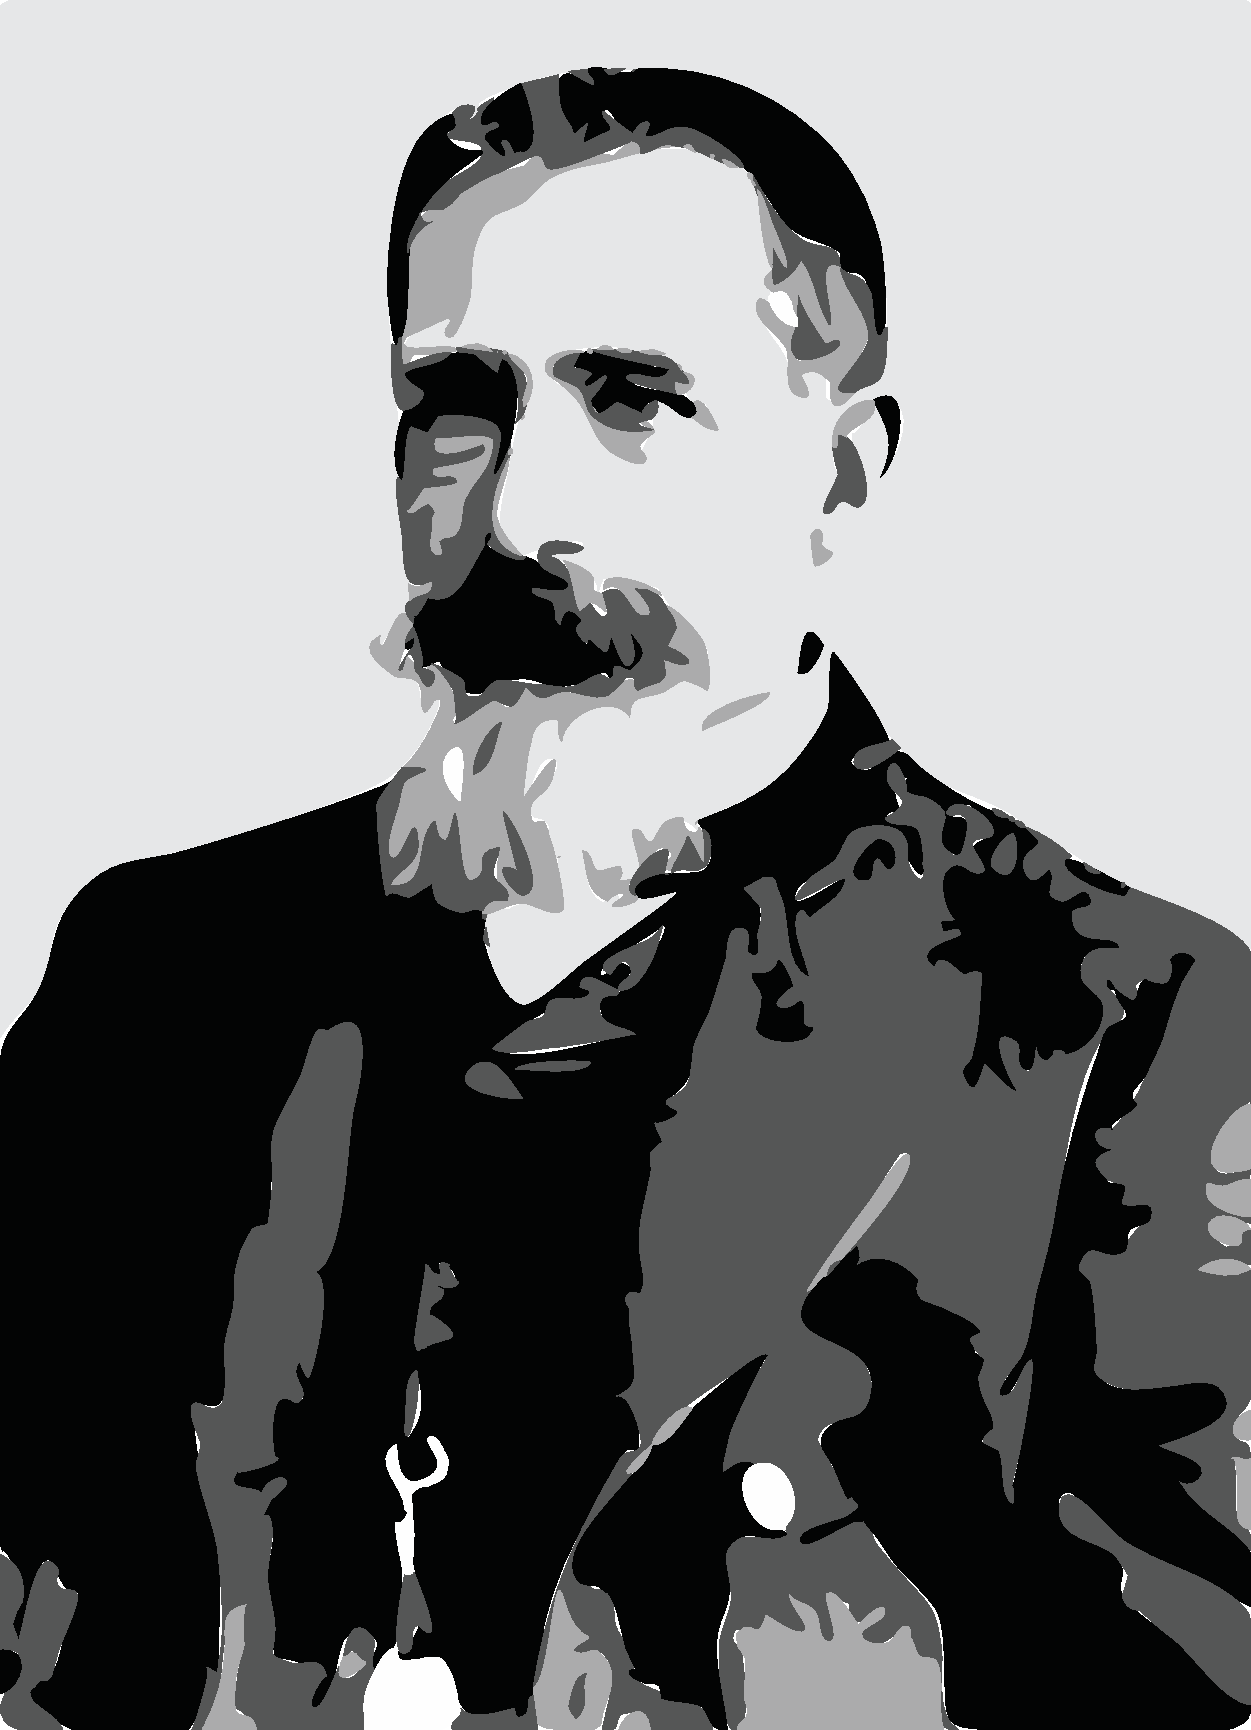
\includegraphics[width=.25\textwidth]{./fotos/calcasdos/Dini.pdf}\\[5pt]
{\small \bfseries Ulisse Dini}
\end{bio}

\begin{theorem}[Dini]
  \label{dini}\index{teorema!de Dini}Sea $K$ un espacio métrico
  compacto y sean $f,f_{k}\in \mathcal{C}^{0}(K)$ tales que
  \begin{equation*}
    f_{1}\leq f_{2}\leq \cdots \leq f_{k}\leq f_{k+1}\leq \cdots
  \end{equation*}
  y
  \begin{equation*}
    f_{k}(x)\rightarrow f(x)\text{ \ para cada }x\in K.
  \end{equation*}
  Entonces $f_{k}\rightarrow f$ uniformemente en $K$.
\end{theorem}

\begin{proof}
  Definimos $g_{k}:=f-f_{k}$. Entonces $g_{k}\geq g_{k+1}\geq 0$ para
  todo $k\in \mathbb{N}$ y
  \begin{equation*}
    \lim_{k\rightarrow \infty }g_{k}(x)=0\text{\qquad }\forall x\in K.
  \end{equation*}
  Sea $\varepsilon >0$. Para cada $x\in K$ elegimos $k_{x}\in
  \mathbb{N}$ tal que
  \begin{equation*}
    g_{k}(x)<\frac{\varepsilon }{2}\text{\qquad }\forall k\geq k_{x}.
  \end{equation*}
  Además, como $g_{k_{x}}$ es continua, existe $\delta_{x}>0$ tal
  que
  \begin{equation*}
    \left\vert g_{k_{x}}(y)-g_{k_{x}}(x)\right\vert <\frac{\varepsilon }{2}\text{\qquad si }d_{K}(y,x)<\delta_{x}.
  \end{equation*}
  Por tanto,
  \begin{equation*}
    g_{k}(y)\leq g_{k_{x}}(y)\leq \left\vert
      g_{k_{x}}(y)-g_{k_{x}}(x)\right\vert +g_{k_{x}}(x)<\varepsilon \text{\qquad
      si \ }k\geq k_{x}\text{ \ y }d_{K}(y,x)<\delta_{x}.
  \end{equation*}
  Como $K$ es compacto, existen $x_{1},\dots,x_{n}\in K$ tales que
  \begin{equation*}
    K\subset B_{K}(x_{1},\delta_{x_{1}})\cup \cdots \cup B_{K}(x_{n},\delta
   _{x_{n}}).
  \end{equation*}
  En consecuencia,
  \begin{equation*}
    g_{k}(y)<\varepsilon \text{\qquad }\forall k\geq \max
    \left\{k_{x_{1}},\dots,k_{x_{n}}\right\},\text{ }\forall y\in K.
  \end{equation*}
  Esto prueba que $f_{k}\rightarrow f$ uniformemente en $K$.
\end{proof}

Una consecuencia importante del teorema de Dini es la siguiente.

\begin{corollary}
  \label{cordini}Sean $f,f_{k}\in \mathcal{C}_{c}^{0}(\mathbb{R}^{n})$
  tales que
  \begin{equation*}
    f_{1}\leq f_{2}\leq \cdots \leq f_{k}\leq f_{k+1}\leq \cdots
  \end{equation*}
  y
  \begin{equation*}
    f_{k}(x)\rightarrow f(x)\text{ \ para cada }x\in \mathbb{R}^{n}.
  \end{equation*}
  Entonces
  \begin{equation*}
    \lim_{k\rightarrow \infty }\int_{\mathbb{R}^{n}}f_{k}=\int_{\mathbb{R}^{n}}f.
  \end{equation*}
\end{corollary}

{\abovedisplayskip=7pt
\belowdisplayskip=7pt
\begin{proof}
  Observa que, si $f(x)=0=f_{1}(x)$, entonces $f_{k}(x)=0$ para todo
  $k\in \mathbb{N}$. En consecuencia, \ sop$(f_{k})\subset $ sop$(f)$
  $\cup $ sop$(f_{1})=:K$ para todo $k\in \mathbb{N}$. Por el
  Teorema~\ref{dini}, $f_{k}\rightarrow f$ uniformemente en $K$ y, por
  tanto, en $\mathbb{R}^{n}$. Aplicando el Lema~\ref{lemhaar1},
  concluimos que
  \begin{equation*}
    \lim_{k\rightarrow \infty }\int_{\mathbb{R}^{n}}f_{k}=\int_{\mathbb{R}^{n}}f,
  \end{equation*}
  como afirma el enunciado.
\end{proof}

Si $f_{k}\in \mathcal{C}_{c}^{0}(\mathbb{R}^{n})$ y $f_{k}\leq
f_{k+1}$, por la monotonía de la integral se tiene que
$\int_{\mathbb{R}^{n}}f_{k}\leq \int_{\mathbb{R}^{n}}f_{k+1}$. De modo
que
\begin{equation*}
  \lim_{k\rightarrow \infty }\int_{\mathbb{R}^{n}}f_{k}=\sup_{k\in \mathbb{N}}\int_{\mathbb{R}^{n}}f_{k}\in \mathbb{R}\cup \left\{\infty \right\}.
\end{equation*}
El siguiente resultado es consecuencia del Corolario~\ref{cordini}.

\begin{corollary}
  \label{indepsuc}Si $f_{k},g_{k}\in
  \mathcal{C}_{c}^{0}(\mathbb{R}^{n})$ cumplen que $f_{k}\leq f_{k+1}$
  y $g_{k}\leq g_{k+1}$ para todo $k\in \mathbb{N}$ y $\sup_{k\in
    \mathbb{N}}f_{k}(x)=\sup_{k\in \mathbb{N}}g_{k}(x)$ para cada
  $x\in \mathbb{R}^{n}$, entonces
  \begin{equation*}
    \lim_{k\rightarrow \infty }\int_{\mathbb{R}^{n}}f_{k}=\lim_{k\rightarrow
      \infty }\int_{\mathbb{R}^{n}}g_{k}.
  \end{equation*}
\end{corollary}

\begin{proof}
  Fija $k\in \mathbb{N}$ y, para cada $j\in \mathbb{N}$, considera la
  función $h_{j}:=\min \left\{f_{k},g_{j}\right\}$. Entonces
  $h_{j}\in \mathcal{C}_{c}^{0}(\mathbb{R}^{n})$ (ver
  Ejercicio~\ref{minmaxenCc}), $\ h_{j}\leq h_{j+1}$,
  $\ f_{k}(x)=\sup_{j\in \mathbb{N}}h_{j}(x)=\lim_{k\rightarrow \infty
  }h_{j}(x)$
  para cada $x\in \mathbb{R}^{n}$ \ y $\ h_{j}\leq g_{j}$. Aplicando
  el Corolario~\ref{cordini} obtenemos
  \begin{equation*}
    \int_{\mathbb{R}^{n}}f_{k}=\lim_{j\rightarrow \infty }\int_{\mathbb{R}^{n}}h_{j}\leq \lim_{j\rightarrow \infty }\int_{\mathbb{R}^{n}}g_{j}\text{\qquad }\forall k\in \mathbb{N}\text{.}
  \end{equation*}
  Por tanto,
  \begin{equation*}
    \lim_{k\rightarrow \infty }\int_{\mathbb{R}^{n}}f_{k}\leq \lim_{j\rightarrow
      \infty }\int_{\mathbb{R}^{n}}g_{j}.
  \end{equation*}
  Intercambiando $f_{k}$ y $g_{k}$ obtenemos el resultado.
\end{proof}

Denotamos por $\mathcal{S}_{\ast }(\mathbb{R}^{n})$ al conjunto de
todas las funciones $f\colon \mathbb{R}^{n}\rightarrow \mathbb{R}\cup
\left\{\infty \right\}$ tales que existe una sucesión de funciones $(f_{k})$
en $\mathcal{C}_{c}^{0}(\mathbb{R}^{n})$ que cumple que $f_{k}\leq
f_{k+1}$ para todo $k\in \mathbb{N}$ y$\ \sup_{k\in
  \mathbb{N}}f_{k}=f$.

\begin{definition}
  \label{defintsci}Si $f\in \mathcal{S}_{\ast }(\mathbb{R}^{n})$
  definimos \textbf{la integral de }$f$\textbf{\ en} $\mathbb{R}^{n}$
  \index{integral!de una función s.c.i.}como
  \begin{equation*}
    \int_{\mathbb{R}^{n}}f:=\lim_{k\rightarrow \infty }\int_{\mathbb{R}^{n}}f_{k}\in \mathbb{R}\cup \left\{\infty \right\},
  \end{equation*}
  donde $(f_{k})$ es una sucesión de funciones en
  $\mathcal{C}_{c}^{0}(\mathbb{R}^{n})$ tales que $f_{k}\leq f_{k+1}$
  para todo $k\in \mathbb{N}$ \ y $\ \sup_{k\in \mathbb{N}}f_{k}=f$.
\end{definition}

El Corolario~\ref{indepsuc}\ asegura que la integral de $f$ en
$\mathbb{R}^{n}$ no depende de la sucesión elegida. En particular,
si $f\in \mathcal{C}_{c}^{0}(\mathbb{R}^{n})\subset \mathcal{S}_{\ast
}(\mathbb{R}^{n})$, podemos tomar $f_{k}=f$. Esto prueba que, para
funciones en $\mathcal{C}_{c}^{0}(\mathbb{R}^{n})$, la integral dada
por la Definición~\ref{defintsci} coincide con la introducida en
el capítulo precedente.

A continuación daremos una descripción más accesible del
conjunto $\mathcal{S}_{\ast }(\mathbb{R}^{n})$. El siguiente lema
muestra que las funciones que pertenecen a $\mathcal{S}_{\ast
}(\mathbb{R}^{n})$ son semicontinuas inferiormente (ver Definición
\ref{defsci}).

Sea $X$ un espacio métrico. El \textbf{supremo puntual}
\index{supremo puntual}de un conjunto de funciones $f_{i}\colon X\rightarrow
\mathbb{R\cup \left\{\infty \right\}}$, $i\in \mathcal{I}$, es la función
\begin{equation*}
  \sup_{i\in \mathcal{I}}f_{i}\colon X\rightarrow \mathbb{R\cup \left\{\infty \right\}}
\end{equation*}
definida como
\begin{equation*}
  \bigl( \sup_{i\in \mathcal{I}}f_{i}\bigr) (x):=\sup_{i\in \mathcal{I}}f_{i}(x)\text{.}
\end{equation*}

\begin{lemma}
  \label{supsci}Si $X$ es un espacio métrico y $f_{i}\colon X\rightarrow
  \mathbb{R\cup \left\{\infty \right\}}$ es s.c.i. para todo $i\in \mathcal{I}$,
  entonces $\sup_{i\in \mathcal{I}}f_{i}$ es s.c.i.
\end{lemma}

\begin{proof}
  Sean $x_{0}\in X$ y $c<\left( \sup_{i\in \mathcal{I}}f_{i}\right)
  (x_{0})$. Escogemos $i_{0}\in \mathcal{I}$ tal que
  $c<f_{i_{0}}(x_{0})$. Como $f_{i_{0}}$ es s.c.i., existe $\delta >0$
  tal que
  \begin{equation*}
    c<f_{i_{0}}(x)\text{\qquad si \ }d_{X}(x,x_{0})<\delta .
  \end{equation*}
  En consecuencia,
  \begin{equation*}
    c<f_{i_{0}}(x)\leq \bigl( \sup_{i\in \mathcal{I}}f_{i}\bigr) (x)\text{\qquad si \ }d_{X}(x,x_{0})<\delta .
  \end{equation*}
  Esto prueba que $\sup_{i\in \mathcal{I}}f_{i}$ es s.c.i.
\end{proof}

El siguiente resultado caracteriza a los elementos de
$\mathcal{S}_{\ast }(\mathbb{R}^{n})$.

\begin{proposition}
  \label{existsci}Sea $f\colon \mathbb{R}^{n}\rightarrow \mathbb{R\cup
    \left\{\infty \right\}}$. Son equivalentes las siguientes afirmaciones:

  \begin{enumerate}
  \item[(a)] $f$ es s.c.i. y existe un compacto $K\subset
    \mathbb{R}^{n}$ tal que
    \begin{equation*}
      f(x)\geq 0\text{\qquad }\forall x\in \mathbb{R}^{n}\smallsetminus K.
    \end{equation*}

  \item[(b)] Existen funciones $f_{k}\in
    \mathcal{C}_{c}^{0}(\mathbb{R}^{n})$ tales que $f_{k}\leq f_{k+1}$
    para todo $k\in \mathbb{N}$ y
    \begin{equation*}
      f=\sup_{k\in \mathbb{N}}f_{k}.
    \end{equation*}
  \end{enumerate}
\end{proposition}}%

\begin{proof}
  \emph{(b)}$\Rightarrow $\emph{(a):} \ Sean $f_{k}\in
  \mathcal{C}_{c}^{0}(\mathbb{R}^{n})$ tales que $f_{k}\leq f_{k+1}$
  para todo $k\in \mathbb{N}$ y $f=\sup_{k\in \mathbb{N}}f_{k}$. El
  Lema~\ref{supsci} asegura que $f$ es s.c.i. Por otra parte, como
  $f\geq f_{1}$, se tiene que
  \begin{equation*}
    f(x)\geq 0\text{\qquad }\forall x\in \mathbb{R}^{n}\smallsetminus \text{ sop}(f_{1}).
  \end{equation*}
  Esto prueba que $f$ cumple \emph{(a)}.

  \emph{(a)}$\Rightarrow $\emph{(b):} \ Sea $f$ s.c.i. y tal que
  $f(x)\geq 0$ para todo $x\in \mathbb{R}^{n}\smallsetminus K$, con
  $K\neq \emptyset $ compacto. Por el Teorema~\ref{sci},\ $f$ alcanza
  su mínimo en $K$. Por tanto, existe $M\in \mathbb{N}$ tal que
  \begin{equation*}
    f(x)>-M\text{\qquad }\forall x\in \mathbb{R}^{n}.
  \end{equation*}
  Sea
  \begin{equation*}
    \mathcal{N}:=\left\{(\xi ,\varepsilon ,q)\in \mathbb{Q}^{n}\times \mathbb{Q}\times \mathbb{Q}:\text{\quad }\varepsilon >0,\text{\quad }q>-M,\text{\quad }f(x)>q\text{ }\forall x\in B(\xi ,\varepsilon )\right\},
  \end{equation*}
  donde $B(\xi ,\varepsilon ):=\left\{x\in \mathbb{R}^{n}:\left\Vert x-\xi
  \right\Vert <\varepsilon \right\}$. Para cada $\nu =(\xi ,\varepsilon
  ,q)\in \mathcal{N}$ escogemos $r_{\nu }\in (\varepsilon ,\infty )$
  tal que $K\subset B(\xi ,r_{\nu })$ y definimos $g_{\nu }\in
  \mathcal{C}_{c}^{0}(\mathbb{R}^{n})$ como
  \begin{equation*}
    g_{\nu }(x):=
      \begin{cases}
        q & \text{si }\left\Vert x-\xi \right\Vert \leq \frac{\varepsilon }{2}, \\ 
        -\frac{2(q+M)}{\varepsilon }\left\Vert x-\xi \right\Vert +2q+M & \text{si }\frac{\varepsilon }{2}\leq \left\Vert x-\xi \right\Vert \leq \varepsilon ,
        \\ 
        -M & \text{si }\varepsilon \leq \left\Vert x-\xi \right\Vert \leq r_{\nu },
        \\ 
        -M(r_{\nu }+1-\left\Vert x-\xi \right\Vert ) & \text{si }r_{\nu }\leq
        \left\Vert x-\xi \right\Vert \leq r_{\nu }+1, \\ 
        0 & \text{si }r_{\nu }+1\leq \left\Vert x-\xi \right\Vert .
      \end{cases}
  \end{equation*}
  \begin{figure}[H]
    \centering
    \begin{tikzpicture}[scale=.3]
  \pgfmathsetmacro{\xO}{1}
  \draw[very thin,-latex'] (-13,0)--(13,0);
  \draw[very thin, -latex'] (-5.5,-5)--(-5.5,10.5);
  \draw[thick] (-11,0)--(-8,0)--(-7,-4)--(-3,-4)--(-1.5,8)--(1.5,8)--(3,-4)--(7,-4)--(8,0)--(11,0);

  \draw[smooth,tension=0.65] plot coordinates{
    (-11,0.1) (-10.5,.15) (-10,.25) (-8.9,.6) (-8,.6) (-7,0) (-5,-2) (-3,3)};
  \draw[smooth,tension=.9] plot coordinates{
    (-3,8.7) (-1.5,9.1) (0,8.6)};
  \draw[smooth,tension=.9] plot coordinates{
    (0, 8.4) (1.6,8.6) (3,9)};
  \draw[smooth,tension=0.6] plot coordinates{
    (3,-1.5) (5,-3) (7,0) (8,.7) (9,0.5) (10,.2) (10.5,.1) (11,0.1)};

\draw[dashed, very thin] (-7,-4)--(-7,0);
\draw[dashed, very thin] (7,-4)--(7,0);
\draw[dashed, very thin] (-3,-4)--(-3,8.7);
\draw[dashed, very thin] (3,-4)--(3,9);
\draw[dashed, very thin] (-5.5,8)--(1.5,8);


  \draw plot[only marks, mark=*,mark size=3pt] coordinates{(-5.5,8) (-5.5,-4) (-8,0 )(-7,0) (-3,0) (0,0)
    (3,0) (7,0) (8,0)};
  \draw (-5.5,8) node[left] {$q$};
  \draw (-5.3,-4) node[below] {$-M$};
  \draw (0,0) node[below] {$\xi$};
\end{tikzpicture}

    % \caption{}
  \end{figure}

  \noindent
  Por construcción, $g_{\nu }\leq f$. Probemos que $\sup_{\nu \in
    \mathcal{N}}g_{\nu }=f$.

  En efecto, como $f$ es s.c.i., dados $x\in \mathbb{R}^{n}$ y $q\in
  \mathbb{Q} $ con $-M<q<f(x)$, existe $\delta >0$ tal que
  \begin{equation*}
    q<f(y)\text{\qquad }\forall y\in B(x,\delta ).
  \end{equation*}
  Tomando $\varepsilon \in \mathbb{Q}\cap (0,\frac{\delta }{2})$ y
  $\xi \in \mathbb{Q}^{n}\cap B(x,\frac{\varepsilon }{2})$, tenemos
  que $B(\xi ,\varepsilon )\subset B(x,\delta )$. Por tanto,
  \begin{equation*}
    q<f(y)\text{\qquad }\forall y\in B(\xi ,\varepsilon )
  \end{equation*}
  y, en consecuencia, $\nu =(\xi ,\varepsilon ,q)\in \mathcal{N}$ y
  $g_{\nu }(x)=q$. Esto prueba que $\sup_{\nu \in \mathcal{N}}g_{\nu
  }=f$.

  El conjunto $\mathcal{N}$\ es numerable. Numeramos sus elementos
  $\mathcal{N}=\left\{\nu_{1},\nu_{2},\dots\right\}$ y definimos
  \begin{equation*}
    f_{k}:=\sup \left\{g_{\nu_{1}},\dots,g_{\nu_{k}}\right\}.
  \end{equation*}
  Entonces $f_{k}\in \mathcal{C}_{c}^{0}(\mathbb{R}^{n})$ (ver
  Ejercicio~\ref{minmaxenCc}), $f_{k}\leq f_{k+1}$ para todo $k\in
  \mathbb{N}$ y $f=\sup_{k\in \mathbb{N}}f_{k}$.
\end{proof}

Como consecuencia de la proposición anterior se tiene
que\index{conjunto!S subestrella@$\mathcal{S}_{\ast
  }(\mathbb{R}^{n})$}
\begin{align*}
  \mathcal{S}_{\ast
  }(\mathbb{R}^{n})=\bigl\{f\colon \mathbb{R}^{n}\rightarrow \mathbb{R}\cup
  \left\{\infty \right\}: &f\text{ es s.c.i. y }\exists K\text{
                            compacto}\\ 
        &\text{tal que }f(x)\geq 0\text{ }\forall x\in \mathbb{R}^{n}\smallsetminus K\bigr\}.
\end{align*}

Procediendo de manera análoga, definiremos la integral de
funciones $f\colon \mathbb{R}^{n}\rightarrow \mathbb{R}\cup \left\{-\infty \right\}$
que son el límite puntual de una sucesión decreciente de
funciones continuas con soporte compacto.

El \textbf{ínfimo puntual} \index{infimo@ínfimo puntual}de un
conjunto de funciones $f_{i}\colon X\rightarrow \mathbb{R\cup \left\{-\infty
  \right\}}$, $i\in \mathcal{I}$, definidas en un espacio métrico $X$ es
la función
\begin{equation*}
  \inf_{i\in \mathcal{I}}f_{i}\colon X\rightarrow \mathbb{R\cup \left\{-\infty \right\}}
\end{equation*}
dada por
\begin{equation*}
  \left( \inf_{i\in \mathcal{I}}f_{i}\right) (x):=\inf_{i\in \mathcal{I}}f_{i}(x)\text{.}
\end{equation*}

Nota que, si definimos $-(-\infty ):=\infty $, las funciones
semicontinuas inferior y superiormente (ver Definición
\ref{defscs}) se relacionan como sigue:
\begin{equation}
  f\colon X\rightarrow \mathbb{R}\cup \left\{-\infty \right\}\text{ es s.c.s. }\quad
  \Longleftrightarrow \quad -f\colon X\rightarrow \mathbb{R}\cup \left\{\infty \right\}\text{
    es s.c.i.}  \label{sci-scs}
\end{equation}
Esta relación, junto con el Lema~\ref{supsci}, implica que el
ínfimo puntual de una familia de funciones semicontinuas
superiormente es semicontinuo superiormente. Además, se tienen los
siguientes resultados.

\begin{corollary}
  \label{indepsuc2}Si $f_{k},g_{k}\in
  \mathcal{C}_{c}^{0}(\mathbb{R}^{n})$ son tales que $f_{k}\geq
  f_{k+1}$ y $g_{k}\geq g_{k+1}$ para todo $k\in \mathbb{N}$ y
  $\inf_{k\in \mathbb{N}}f_{k}=\inf_{k\in \mathbb{N}}g_{k}$, entonces
  \begin{equation*}
    \lim_{k\rightarrow \infty }\int_{\mathbb{R}^{n}}f_{k}=\lim_{k\rightarrow
      \infty }\int_{\mathbb{R}^{n}}g_{k}.
  \end{equation*}
\end{corollary}

\begin{proof}
  Esta afirmación es consecuencia inmediata del
  Corolario~\ref{indepsuc}, aplicado a las sucesiones $(-f_{k})$ y
  $(-g_{k})$, y la relación (\ref{sci-scs}).
\end{proof}

\begin{proposition}
  \label{existscs}Sea $f\colon \mathbb{R}^{n}\rightarrow \mathbb{R}\cup
  \left\{-\infty \right\}$. Son equivalentes las siguientes afirmaciones:

  \begin{enumerate}
  \item[(a)] $f$ es s.c.s. y existe un compacto $K\subset
    \mathbb{R}^{n}$ tal que
    \begin{equation*}
      f(x)\leq 0\text{\qquad }\forall x\in \mathbb{R}^{n}\smallsetminus K.
    \end{equation*}

  \item[(b)] Existen funciones $f_{k}\in
    \mathcal{C}_{c}^{0}(\mathbb{R}^{n})$ tales que $f_{k}\geq f_{k+1}$
    para todo $k\in \mathbb{N}$ y
    \begin{equation*}
      f=\inf_{k\in \mathbb{N}}f_{k}.
    \end{equation*}
  \end{enumerate}
\end{proposition}

\begin{proof}
  De la relación (\ref{sci-scs}) y la Proposición~\ref{existsci} se
  sigue inmediatamente este resultado.
\end{proof}

Denotamos por\index{conjunto!S superestrella@$\mathcal{S}^{\ast
  }(\mathbb{R}^{n})$}
\begin{align*}
  \mathcal{S}^{\ast
  }(\mathbb{R}^{n}):=\bigl\{f\colon \mathbb{R}^{n}\rightarrow \mathbb{R}\cup
  \left\{-\infty \right\}: &f\text{ es s.c.s. y }\exists K\text{
  compacto}\\ 
  &\text{tal que }f(x)\leq 0\text{ }\forall x\in \mathbb{R}^{n}\smallsetminus K\bigr\}.
\end{align*}

\begin{definition}
  \label{defintscs}Sea $f\in \mathcal{S}^{\ast }(\mathbb{R}^{n})$.
  Definimos \textbf{la integral de }$f$\textbf{\ en} $\mathbb{R}^{n}$
  \index{integral!de una función s.c.s.}como
  \begin{equation*}
    \int_{\mathbb{R}^{n}}f:=\lim_{k\rightarrow \infty }\int_{\mathbb{R}^{n}}f_{k}\in \mathbb{R}\cup \left\{-\infty \right\},
  \end{equation*}
  donde $(f_{k})$ es una sucesión de funciones en
  $\mathcal{C}_{c}^{0}(\mathbb{R}^{n})$ tales que $f_{k}\geq f_{k+1}$
  para todo $k\in \mathbb{N}$ \ y $\inf_{k\in \mathbb{N}}f_{k}=f$.
\end{definition}

La Proposición~\ref{existscs}\ asegura que tal sucesión
$(f_{k})$ existe y el Corolario~\ref{indepsuc2}\ asegura que la
integral de $f$ en $\mathbb{R}^{n}$ no depende de la sucesión
elegida. En particular, si $f\in
\mathcal{C}_{c}^{0}(\mathbb{R}^{n})\subset \mathcal{S}^{\ast
}(\mathbb{R}^{n})$, podemos tomar $f_{k}=f$. Esto prueba que, para
funciones en $\mathcal{C}_{c}^{0}(\mathbb{R}^{n})$, la integral dada
por la Definición~\ref{defintscs} coincide con la introducida en
el capítulo precedente. Más aún, como
\begin{equation*}
  \mathcal{S}^{\ast }(\mathbb{R}^{n})\cap \mathcal{S}_{\ast }(\mathbb{R}^{n})=\mathcal{C}_{c}^{0}(\mathbb{R}^{n}),
\end{equation*}
las integrales dadas por las Definiciones~\ref{defintsci} y
\ref{defintscs} coinciden en $\mathcal{S}^{\ast }(\mathbb{R}^{n})\cap
\mathcal{S}_{\ast }(\mathbb{R}^{n})$.

\section{Propiedades de la integral de funciones semicontinuas}

Probaremos algunas propiedades importantes de la integral. Empezamos
con la siguiente observación sencilla. Como antes, convenimos que
$-(-\infty ):=\infty $.

{\abovedisplayskip=8pt
\belowdisplayskip=8pt
\begin{lemma}
  \label{rel}$f\in \mathcal{S}_{\ast }(\mathbb{R}^{n})$ si y sólo
  si $-f\in \mathcal{S}^{\ast }(\mathbb{R}^{n})$. En este caso,
  \begin{equation*}
    \int_{\mathbb{R}^{n}}f=-\int_{\mathbb{R}^{n}}\left( -f\right) .
  \end{equation*}
\end{lemma}

\begin{proof}
  Observa que $f_{k}\in \mathcal{C}_{c}^{0}(\mathbb{R}^{n})$,
  $f_{k}\leq f_{k+1}$ y $\sup_{k\in \mathbb{N}}f_{k}=f$ si y sólo si
  $-f_{k}\in \mathcal{C}_{c}^{0}(\mathbb{R}^{n})$,
  $-f_{k}\geq -f_{k+1}$ y $\inf_{k\in \mathbb{N}}(-f_{k})=-f$. Por el
  Teorema~\ref{haar},
  \begin{equation*}
    \int_{\mathbb{R}^{n}}f_{k}=-\int_{\mathbb{R}^{n}}\left( -f_{k}\right) .
  \end{equation*}
  Pasando al límite obtenemos la identidad deseada.
\end{proof}

Si $f,g\in \mathcal{S}_{\ast }(\mathbb{R}^{n})$ o $f,g\in
\mathcal{S}^{\ast }(\mathbb{R}^{n})$ y $\lambda \in [0,\infty
)$, definimos
\begin{equation*}
  \left( f+g\right) (x):=f(x)+g(x),\text{\qquad }\left( \lambda f\right) (x):=\lambda f(x),
\end{equation*}
donde
  \begin{alignat*}{4}
    a+\infty &:=\infty &\quad&\text{y}& \infty +a&:=\infty &\quad&\forall
    a\in \mathbb{R}\cup \left\{\infty \right\}, \\ 
    a+\left( -\infty \right) &:=-\infty &&\text{y} &\quad\left( -\infty
    \right) +a&:=-\infty &&\forall a\in \mathbb{R}\cup \left\{-\infty \right\}, \\ 
    \lambda \left( \infty \right) &:=\infty &&\text{y}&\lambda
    \left( -\infty \right)&:=-\infty &&\forall \lambda \in (0,\infty ), \\ 
    0\left( \pm \infty \right) &:=0. &&  &&  && 
  \end{alignat*}
Estas definiciones no son arbitrarias: $\infty $ es, por
definición, el supremo de cualquier sucesión no decreciente y
no acotada de números reales. Si a una sucesión de este tipo
le sumamos un número real, o si la multiplicamos por un número
positivo, obtenemos nuevamente una sucesión de este tipo. Mientras
que, si la multiplicamos por $0$, obtenemos la sucesión constante
igual a $0$. Las otras definiciones se obtienen de manera
análoga. Nota, en cambio, que ``$\infty -\infty$'' no está
definido.

Ni $\mathcal{S}^{\ast }(\mathbb{R}^{n})$ ni $\mathcal{S}_{\ast
}(\mathbb{R}^{n})$ son espacios vectoriales. Sin embargo, se cumple lo
siguiente.

\begin{proposition}
  \label{linmonsc}

  \begin{enumerate}
  \item[(a)] Si $f,g\in \mathcal{S}_{\ast }(\mathbb{R}^{n})$ y
    $\lambda \in [0,\infty )$, entonces $f+g\in
    \mathcal{S}_{\ast }(\mathbb{R}^{n})$, $\lambda f\in
    \mathcal{S}_{\ast }(\mathbb{R}^{n})$,
    \begin{equation*}
      \int_{\mathbb{R}^{n}}\left( f+g\right) =\int_{\mathbb{R}^{n}}f+\int_{\mathbb{R}^{n}}g\text{\qquad y\qquad }\int_{\mathbb{R}^{n}}\left( \lambda f\right)
      =\lambda \int_{\mathbb{R}^{n}}f.
    \end{equation*}

  \item[(b)] Si $f,g\in \mathcal{S}_{\ast }(\mathbb{R}^{n})$ y $f\leq
    g$, entonces
    \begin{equation*}
      \int_{\mathbb{R}^{n}}f\leq \int_{\mathbb{R}^{n}}g.
    \end{equation*}
  \end{enumerate}

  Ambas afirmaciones también son ciertas si reemplazamos
  $\mathcal{S}_{\ast }(\mathbb{R}^{n})$ por $\mathcal{S}^{\ast
  }(\mathbb{R}^{n})$.
\end{proposition}

\begin{proof}
  Demostraremos ambas afirmaciones para $\mathcal{S}_{\ast
  }(\mathbb{R}^{n})$. El resultado para $\mathcal{S}^{\ast
  }(\mathbb{R}^{n})$ se obtiene aplicando el Lema~\ref{rel}.

  \emph{(a):} \ Si $f_{k},g_{k}\in
  \mathcal{C}_{c}^{0}(\mathbb{R}^{n})$ son tales que $f_{k}\leq
  f_{k+1}$, $g_{k}\leq g_{k+1}$, $\sup_{k\in \mathbb{N}}f_{k}=f$ \ y
  $\ \sup_{k\in \mathbb{N}}g_{k}=g$, entonces
  \begin{equation*}
    f_{k}+g_{k}\in \mathcal{C}_{c}^{0}(\mathbb{R}^{n}),\text{\qquad }f_{k}+g_{k}\leq f_{k+1}+g_{k+1},\text{\qquad }\sup_{k\in \mathbb{N}}\left(
      f_{k}+g_{k}\right) =f+g,
  \end{equation*}
  y para $\lambda \in [0,\infty )$
  \begin{equation*}
    \lambda f_{k}\in \mathcal{C}_{c}^{0}(\mathbb{R}^{n}),\qquad \lambda
    f_{k}\leq \lambda f_{k+1},\qquad \sup_{k\in \mathbb{N}}\left( \lambda
      f_{k}\right) =\lambda f.
  \end{equation*}
  Del Teorema~\ref{existsci} se sigue que $f+g\in \mathcal{S}_{\ast
  }(\mathbb{R}^{n})$ y $\lambda f\in \mathcal{S}_{\ast
  }(\mathbb{R}^{n})$, y las identidades
  \begin{equation*}
    \int_{\mathbb{R}^{n}}\left( f+g\right) =\int_{\mathbb{R}^{n}}f+\int_{\mathbb{R}^{n}}g\text{\qquad y\qquad }\int_{\mathbb{R}^{n}}\lambda f=\lambda \int_{\mathbb{R}^{n}}f
  \end{equation*}
  son consecuencia de las correspondientes identidades para las
  funciones $f_{k},g_{k}\in \mathcal{C}_{c}^{0}(\mathbb{R}^{n})$ (ver
  Teorema~\ref{haar}).

  \emph{(b):} \ Si $f,g\in \mathcal{S}_{\ast }(\mathbb{R}^{n})$,
  $f\leq g$, y $f_{k},g_{k}\in \mathcal{C}_{c}^{0}(\mathbb{R}^{n})$
  son tales que $f_{k}\leq f_{k+1}$, $g_{k}\leq g_{k+1}$, $\sup_{k\in
    \mathbb{N}}f_{k}=f$ y $\sup_{k\in \mathbb{N}}g_{k}=g$, definimos
  \begin{equation*}
    h_{k}:=\min \left\{f_{k},g_{k}\right\}.
  \end{equation*}
  Entonces $h_{k}\in \mathcal{C}_{c}^{0}(\mathbb{R}^{n})$, $\
  h_{k}\leq h_{k+1} $, $\ \sup_{k\in \mathbb{N}}h_{k}=f$ \ y $\
  h_{k}\leq g_{k}$. De la monotonía de la integral para funciones
  en $\mathcal{C}_{c}^{0}(\mathbb{R}^{n}) $ (ver Teorema~\ref{haar})
  se sigue que
  \begin{equation*}
    \int_{\mathbb{R}^{n}}f:=\lim_{k\rightarrow \infty }\int_{\mathbb{R}^{n}}h_{k}\leq \lim_{k\rightarrow \infty }\int_{\mathbb{R}^{n}}g_{k}=:\int_{\mathbb{R}^{n}}g.
  \end{equation*}
  Esto concluye la demostración.
\end{proof}

Una consecuencia que nos será de utilidad más adelante es la
siguiente.

\begin{corollary}
  \label{correl}Si $f\in \mathcal{S}_{\ast }(\mathbb{R}^{n})$ y $g\in
  \mathcal{S}^{\ast }(\mathbb{R}^{n})$, entonces $f-g\in
  \mathcal{S}_{\ast }(\mathbb{R}^{n})$ y
  \begin{equation*}
    \int_{\mathbb{R}^{n}}(f-g)=\int_{\mathbb{R}^{n}}f-\int_{\mathbb{R}^{n}}g.
  \end{equation*}
\end{corollary}

\begin{proof}
  El Lema~\ref{rel}\ y la Proposición~\ref{linmonsc}\ implican que
  $-g\in \mathcal{S}_{\ast }(\mathbb{R}^{n})$, $f-g\in
  \mathcal{S}_{\ast }(\mathbb{R}^{n})$ y
  \begin{equation*}
    \int_{\mathbb{R}^{n}}(f-g)=\int_{\mathbb{R}^{n}}f+\int_{\mathbb{R}^{n}}\left( -g\right) =\int_{\mathbb{R}^{n}}f-\int_{\mathbb{R}^{n}}g,
  \end{equation*}
  como afirma el enunciado.
\end{proof}

Se cumple además lo siguiente.

\begin{proposition}
  \label{cvsc}Si $A\in GL(n,\mathbb{R})$, $\zeta \in \mathbb{R}^{n}$ y
  $f\in \mathcal{S}_{\ast }(\mathbb{R}^{n})$, entonces la función
  $x\mapsto f(Ax+\zeta )$ pertenece a $\mathcal{S}_{\ast
  }(\mathbb{R}^{n})$ y
  \begin{equation*}
    \int_{\mathbb{R}^{n}}f(Ax+\zeta )\left\vert \det A\right\vert dx=\int_{\mathbb{R}^{n}}f(y)dy.
  \end{equation*}
  La afirmación también es cierta si reemplazamos
  $\mathcal{S}_{\ast }(\mathbb{R}^{n})$ por $\mathcal{S}^{\ast
  }(\mathbb{R}^{n})$.
\end{proposition}

\begin{proof}
  Si $f=\sup_{k\in \mathbb{N}}f_{k}$ con $f_{k}\in
  \mathcal{C}_{c}^{0}(\mathbb{R}^{n})$ y $f_{k}\leq f_{k+1}$, y si
  denotamos por $\varphi (x):=Ax+\zeta $, entonces $f_{k}\circ \varphi
  \in \mathcal{C}_{c}^{0}(\mathbb{R}^{n})$, $\ f_{k}\circ \varphi \leq
  f_{k+1}\circ \varphi $ \ y $\ f\circ \varphi =\sup_{k\in
    \mathbb{N}}\left( f_{k}\circ \varphi \right) $. Así que
  $f\circ \varphi \in \mathcal{S}_{\ast }(\mathbb{R}^{n})$ y el
  resultado es consecuencia inmediata del Teorema~\ref{cvlin}.
\end{proof}

Para $1\leq m<n$, identificamos a $\mathbb{R}^{n}$ con
$\mathbb{R}^{m}\times \mathbb{R}^{n-m}$ y denotamos a un punto $x\in
\mathbb{R}^{n}$ como $x=(y,z)$ con $y\in \mathbb{R}^{m}$ y $z\in
\mathbb{R}^{n-m}$.

Si $g\colon \mathbb{R}^{m}\rightarrow \mathbb{R\cup \left\{\infty \right\}}$,
$h\colon \mathbb{R}^{n-m}\rightarrow \mathbb{R\cup \left\{\infty \right\}}$,
 $g\geq 0$, $h\geq 0$, 
definimos\linebreak $g\odot h\colon \mathbb{R}^{n}\rightarrow
\mathbb{R\cup \left\{\infty \right\}}$ como
\begin{equation*}
  \left( g\odot h\right) (y,z):=g(y)h(z),
\end{equation*}
donde $(\mathbb{\infty )(\infty )}:=\mathbb{\infty }$.

\begin{proposition}
  \label{propprodtens}Sean $g\in \mathcal{S}_{\ast }(\mathbb{R}^{m})$
  y $h\in \mathcal{S}_{\ast }(\mathbb{R}^{n-m})$ tales que $g\geq 0$ y
  $h\geq 0$. Entonces $g\odot h\in \mathcal{S}_{\ast
  }(\mathbb{R}^{n})$ y
  \begin{equation*}
    \int_{\mathbb{R}^{n}}\left( g\odot h\right) =\biggl( \int_{\mathbb{R}^{m}}g\biggr) \biggl( \int_{\mathbb{R}^{n-m}}h\biggr) .
  \end{equation*}
  La afirmación también es cierta si reemplazamos
  $\mathcal{S}_{\ast }$ por $\mathcal{S}^{\ast }$.
\end{proposition}

\begin{proof}
  Demostraremos el resultado para $\mathcal{S}_{\ast }$. La
  demostración para $\mathcal{S}^{\ast }$ es más sencilla.

  Sean $g_{k}\in \mathcal{C}_{c}^{0}(\mathbb{R}^{m})$ y $h_{k}\in
  \mathcal{C}_{c}^{0}(\mathbb{R}^{n-m})$ tales que $g_{k}\leq
  g_{k+1}$, $h_{k}\leq h_{k+1} $, $\ g=\sup_{k\in \mathbb{N}}g_{k}$ y
  $h=\sup_{k\in \mathbb{N}}h_{k}$. Sustituyendo, de ser necesario,
  $g_{k}$ por $\max \left\{g_{k},0\right\}$ y $h_{k}$ por $\max \left\{h_{k},0\right\}$,
  podemos suponer que $g_{k}\geq 0$ y $h_{k}\geq 0$. Se tiene entonces
  que $g_{k}\odot h_{k}\in \mathcal{C}_{c}^{0}(\mathbb{R}^{n})$, $\
  g_{k}\odot h_{k}\leq g_{k+1}\odot h_{k+1}$ \ y $g\odot h=\sup_{k\in
    \mathbb{N}}(g_{k}\odot h_{k})$. Usando el Ejercicio~\ref{intprodtens} obtenemos
  \begin{align*}
    \int_{\mathbb{R}^{n}}\left( g\odot h\right) &=\lim_{k\rightarrow \infty
    }\int_{\mathbb{R}^{n}}\left( g_{k}\odot h_{k}\right) \\
    &=\lim_{k\rightarrow \infty }\left[ \biggl( \int_{\mathbb{R}^{m}}g_{k}\biggr) \biggl( \int_{\mathbb{R}^{n-m}}h_{k}\biggr) \right] =\biggl(
      \int_{\mathbb{R}^{m}}g\biggr) \biggl( \int_{\mathbb{R}^{n-m}}h\biggr) ,
  \end{align*}
  como afirma el enunciado.
\end{proof}

El siguiente resultado asegura que la integral se obtiene integrando
sucesivamente respecto a cada variable.

Dada una función $f\colon \mathbb{R}^{n}\rightarrow \mathbb{R}\cup \left\{\pm
\infty \right\}$ y un punto $z\in \mathbb{R}^{n-m}$, denotamos por
$f^{z}\colon \mathbb{R}^{m}\rightarrow \mathbb{R}\cup \left\{\pm \infty \right\}$ a la
función
\begin{equation*}
  f^{z}(y):=f(y,z).
\end{equation*}

\begin{proposition}[Teorema de Fubini para funciones semicontinuas]
  \label{propfub}Sean $1\leq m<n$ y $f\in \mathcal{S}_{\ast
  }(\mathbb{R}^{n})$. Entonces, para cada $z\in \mathbb{R}^{n-m}$, la
  función $f^{z}$ pertenece a $\mathcal{S}_{\ast
  }(\mathbb{R}^{m})$, la función $F\colon \mathbb{R}^{n-m}\rightarrow
  \mathbb{R}\cup \left\{\infty \right\}$ dada por
  \begin{equation*}
    F(z):=\int_{\mathbb{R}^{m}}f^{z}
  \end{equation*}
  pertenece a $\mathcal{S}_{\ast }(\mathbb{R}^{n-m})$ y
  \begin{equation}
    \int_{\mathbb{R}^{n-m}}F=\int_{\mathbb{R}^{n}}f.  \label{fub0}
  \end{equation}
  La afirmación también es cierta si reemplazamos
  $\mathcal{S}_{\ast }$ por $\mathcal{S}^{\ast }$ y $\infty $ por
  $-\infty $.
\end{proposition}}%

\begin{proof}
  Probaremos la afirmación para $f\in \mathcal{S}_{\ast
  }(\mathbb{R}^{n})$. La afirmación para $f\in \mathcal{S}^{\ast
  }(\mathbb{R}^{n})$ se obtiene aplicando el Lema~\ref{rel}.

  Sea $(f_{k})$ una sucesión en
  $\mathcal{C}_{c}^{0}(\mathbb{R}^{n})$ tal que $f_{k}\leq f_{k+1}$ \
  y $\ f=\sup_{k\in \mathbb{N}}f_{k}$. Entonces, para cada $z\in
  \mathbb{R}^{n-m}$, se cumple que $f_{k}^{z}\in
  \mathcal{C}_{c}^{0}(\mathbb{R}^{m})$, $f_{k}^{z}\leq f_{k+1}^{z}$ \
  y $\ f^{z}=\sup_{k\in \mathbb{N}}f_{k}^{z}$. En consecuencia,
  $f^{z}\in \mathcal{S}_{\ast }(\mathbb{R}^{m})$ y
  \begin{equation}
    F(z):=\int_{\mathbb{R}^{m}}f^{z}=\lim_{k\rightarrow \infty }\int_{\mathbb{R}^{m}}f_{k}^{z}=\lim_{k\rightarrow \infty }F_{k}(z),  \label{Flim}
  \end{equation}
  donde $F_{k}\colon \mathbb{R}^{n-m}\rightarrow \mathbb{R}$ es la
  función dada por
  \begin{equation*}
    F_{k}(z):=\int_{\mathbb{R}^{m}}f_{k}^{z}.
  \end{equation*}
  Esta función es continua (ver Lema~\ref{basico}). Además, si
  sop$(f_{k})\subset [a_{1},b_{1}]\times \cdots \times [a_{n},b_{n}]$ y $z\notin [a_{m+1},b_{m+1}]\times \cdots
  \times [a_{n},b_{n}]$, entonces $f_{k}^{z}=0$ y, en
  consecuencia, $F_{k}(z)=0$. Por tanto, $F_{k}\in
  \mathcal{C}_{c}^{0}(\mathbb{R}^{n-m})$. De la monotonía de la
  integral se sigue que $F_{k}\leq F_{k+1}$ y la igualdad (\ref{Flim})
  afirma que $F=\sup_{k\in \mathbb{N}}F_{k}$. Esto implica que $F\in
  \mathcal{S}_{\ast }(\mathbb{R}^{n-m})$ y
  \begin{equation}
    \int_{\mathbb{R}^{n-m}}F=\lim_{k\rightarrow \infty }\int_{\mathbb{R}^{n-m}}F_{k}.  \label{fub1}
  \end{equation}
  Por otra parte, de la definición de la integral en
  $\mathcal{C}_{c}^{0}(\mathbb{R}^{n})$ se sigue que
  \begin{align}
    \int_{\mathbb{R}^{n-m}}F_{k}(z)dz &=\int_{\mathbb{R}^{n-m}}\biggl( \int_{\mathbb{R}^{m}}f_{k}^{z}(y)dy\biggr) dz  \notag \\
    &=\int_{\mathbb{R}^{n-m}}\biggl( \int_{\mathbb{R}^{m}}f_{k}(y,z)dy\biggr) dz
    \notag \\
    &=\int_{\mathbb{R}^{n}}f_{k}(x_{1},\dots,x_{n})dx_{1}\cdots dx_{n}.
    \label{fub2}
  \end{align}
  De las identidades (\ref{fub1}) y (\ref{fub2}) se obtiene
  \begin{equation*}
    \int_{\mathbb{R}^{n-m}}F=\lim_{k\rightarrow \infty }\int_{\mathbb{R}^{n}}f_{k}=\int_{\mathbb{R}^{n}}f,
  \end{equation*}
  como afirma el enunciado.
\end{proof}

Nota que, por la invariancia de la integral bajo isometrías
(Proposición~\ref{cvsc}), podemos intercambiar el orden de las
integrales en la proposición anterior, es decir, integrar primero
respecto a $z$ y después respecto a $y$. Las identidades
correspondientes (\ref{fub0}) suelen escribirse como
\begin{align}
  \int_{\mathbb{R}^{n-m}}\biggl( \int_{\mathbb{R}^{m}}f(y,z)dy\biggr)
  dz &=\int_{\mathbb{R}^{n}}f(y,z)dy\,dz \notag \\
  &=\int_{\mathbb{R}^{m}}\biggl( \int_{\mathbb{R}^{n-m}}f(y,z)dz\biggr) dy.  \label{idfub}
\end{align}

Un primer resultado que permite el intercambio del límite puntual
de funciones con la integral es el siguiente.

\begin{proposition}[Convergencia monótona para funciones
  semicontinuas]
  \label{cmsci}Sea $(f_{k})$ una sucesión en $\mathcal{S}_{\ast
  }(\mathbb{R}^{n})$ tal que $f_{k}\leq f_{k+1}$ para todo $k\in
  \mathbb{N}$ y $f:=\sup_{k\in \mathbb{N}}f_{k}$. Entonces $f\in
  \mathcal{S}_{\ast }(\mathbb{R}^{n})$ y
  \begin{equation*}
    \int_{\mathbb{R}^{n}}f=\lim_{k\rightarrow \infty }\int_{\mathbb{R}^{n}}f_{k}.
  \end{equation*}
\end{proposition}

\begin{proof}
  Para cada $k\in \mathbb{N}$, tomemos una sucesión $(f_{k,j})$ en
  $\mathcal{C}_{c}^{0}(\mathbb{R}^{n})$ tal que $f_{k,j}\leq
  f_{k,j+1}$ para todo $j\in \mathbb{N}$ y $f_{k}:=\sup_{j\in
    \mathbb{N}}f_{k,j}$. Observa que
  \begin{equation*}
    f_{i,j}\leq f_{i}\leq f_{k}\text{\qquad }\forall j\in \mathbb{N}\text{, }\forall i\leq k.
  \end{equation*}
  Definimos
  \begin{equation*}
    g_{k}:=\max_{i\leq k,\text{ }j\leq k}f_{i,j}.
  \end{equation*}
  Entonces $g_{k}\in \mathcal{C}_{c}^{0}(\mathbb{R}^{n})$, $g_{k}\leq
  g_{k+1}$ y $g_{k}\leq f_{k}$ para todo $k\in \mathbb{N}$, y
  \begin{equation*}
    f=\sup_{k\in \mathbb{N}}f_{k}=\sup_{i,j\in \mathbb{N}}f_{i,j}=\sup_{k\in 
      \mathbb{N}}g_{k}.
  \end{equation*}
  En consecuencia, $f\in \mathcal{S}_{\ast }(\mathbb{R}^{n})$ y de la
  monotonía de la integral (Proposición~\ref{linmonsc}) se
  sigue que
  \begin{equation*}
    \int_{\mathbb{R}^{n}}f_{i}\leq \int_{\mathbb{R}^{n}}f=\lim_{k\rightarrow
      \infty }\int_{\mathbb{R}^{n}}g_{k}\leq \lim_{k\rightarrow \infty }\int_{\mathbb{R}^{n}}f_{k}.
  \end{equation*}
  Pasando al límite obtenemos que
  \begin{equation*}
    \int_{\mathbb{R}^{n}}f=\lim_{k\rightarrow \infty }\int_{\mathbb{R}^{n}}f_{k},
  \end{equation*}
  como afirma el enunciado.
\end{proof}

\section{El volumen de un conjunto}

Aplicaremos las propiedades de la integral para calcular el volumen de
algunos subconjuntos de $\mathbb{R}^{n}$. Empecemos definiendo este
concepto.

\begin{definition}
  \label{funcar}La \textbf{función característica} (o
  \textbf{función indicadora})
  \index{función!característica@característica
    $1_{X}$}de un subconjunto $X$ de $\mathbb{R}^{n}$ es la
  función
  \begin{equation*}
    1_{X}(x):=
      \begin{cases}
        1 & 
        \text{si $x\in X$,} \\ 
        0 & \text{si $x\in \mathbb{R}^{n}\smallsetminus X$.}
      \end{cases}
  \end{equation*}
\end{definition}

Es sencillo comprobar que la función $1_{X}$ es s.c.i si y
sólo si $X $ es abierto en $\mathbb{R}^{n}$, y es s.c.s. si y
sólo si $X$ es cerrado en $\mathbb{R}^{n}$. En consecuencia,
\begin{align}
  1_{X} &\in \mathcal{S}_{\ast }(\mathbb{R}^{n})\text{ si y sólo si }X\text{ es abierto en }\mathbb{R}^{n},  \label{indsci} \\
  1_{X} &\in \mathcal{S}^{\ast }(\mathbb{R}^{n})\text{ si y sólo si }X\text{ es compacto en }\mathbb{R}^{n}.  \label{indscs}
\end{align}
Proponemos la demostración de estas afirmaciones como ejercicio
[Ejercicio~\ref{indsc}].

\begin{definition}
  \label{volabcom}Si $X$ es un subconjunto abierto o $X$ es un
  subconjunto compacto de $\mathbb{R}^{n}$, definimos el
  \textbf{volumen de} $X$ en $\mathbb{R}^{n}$ \index{volumen}como
  \begin{equation*}
    \vol_{n}(X):=\int_{\mathbb{R}^{n}}1_{X} \;\in \mathbb{R}\cup
    \left\{\infty \right\}.
  \end{equation*}
\end{definition}

El volumen tiene las siguientes propiedades.

\begin{proposition}
  \label{propvol}

  \begin{enumerate}
  \item[(a)] Si $X\subset Y$ son subconjuntos de $\mathbb{R}^{n}$ y
    ambos son abiertos o ambos son compactos, entonces
    \begin{equation*}
      \vol_{n}(X)\leq \vol_{n}(Y).
    \end{equation*}

  \item[(b)] Sea $\varphi (x)=Ax+\zeta $ con $A\in GL(n,\mathbb{R})$,
    $\zeta \in \mathbb{R}^{n}$. Entonces $\varphi (X):=\left\{\varphi
    (x):x\in X\right\}$ es un subconjunto abierto de $\mathbb{R}^{n}$ si $X$
    lo es, y $\varphi (X)$ es compacto si $X$ lo es. En ambos casos,
    \begin{equation*}
      \vol_{n}(\varphi (X))=\left\vert \det A\right\vert \,\vol_{n}(X).
    \end{equation*}
  \end{enumerate}
\end{proposition}

\begin{proof}
  \emph{(a):} \ Si $X\subset Y$ entonces $1_{X}\leq 1_{Y}$.
  Además, $1_{X},1_{Y}\in \mathcal{S}_{\ast }(\mathbb{R}^{n})$ si
  $X$ y $Y$ son abiertos, y $1_{X},1_{Y}\in \mathcal{S}^{\ast
  }(\mathbb{R}^{n})$ si $X$ y $Y$ son compactos. Así que en ambos
  casos podemos aplicar la afirmación \emph{(b)}\ de la
  Proposición~\ref{linmonsc} para obtener la afirmación
  deseada.

  \emph{(b):} \ Como $\varphi $ es un homeomorfismo, $\varphi (X)$ es
  abierto si $X$ lo es y $\varphi (X)$ es compacto si $X$ lo es. Nota
  que $1_{\varphi (X)}\circ \varphi =1_{X}$. Las
  Proposiciones~\ref{linmonsc} y~\ref{cvsc} aseguran entonces que
  \begin{equation*}
    \left\vert \det A\right\vert \int_{\mathbb{R}^{n}}1_{X}=\int_{\mathbb{R}^{n}}\left( 1_{\varphi (X)}\circ \varphi \right) \left\vert \det
      A\right\vert =\int_{\mathbb{R}^{n}}1_{\varphi (X)},
  \end{equation*}
  como afirma el enunciado.
\end{proof}

Veamos algunos ejemplos.

\begin{example}
  \label{para}

  \begin{enumerate}
  \item[(a)] Si $U=\left( a_{1},b_{1}\right) \times \cdots \times
    \left( a_{n},b_{n}\right) $ con $a_{i},b_{i}\in \mathbb{R}$,
    $a_{i}<b_{i}$, entonces
    \begin{equation*}
      \vol_{n}(U)=\prod_{i=1}^{n}(b_{i}-a_{i}).
    \end{equation*}

  \item[(b)] Si $Q=[a_{1},b_{1}]\times \cdots \times [a_{n},b_{n}]$ con $a_{i},b_{i}\in \mathbb{R}$, $a_{i}\leq b_{i}$,
    entonces
    \begin{equation*}
      \vol_{n}(Q)=\prod_{i=1}^{n}(b_{i}-a_{i}).
    \end{equation*}
    En particular, si $a_{i}=b_{i}$ para algún $i=1,\dots,n$,
    entonces $\vol_{n}(Q)=0$.
  \end{enumerate}
\end{example}

\begin{proof}
  \emph{(a):} \ En el Ejemplo~\ref{volcubab}\ probamos que
  \begin{equation*}
    \vol_{1}((0,1))=1.
  \end{equation*}
  Si $a,b\in \mathbb{R}$, $a\leq b$, y $\varphi \colon \mathbb{R}\rightarrow
  \mathbb{R}$ es la función $\varphi (t):=(b-a)t+a$, entonces
  $\varphi ((0,1))=(a,b)$ y la Proposición~\ref{propvol}\ asegura
  que
  \begin{equation*}
    \vol_{1}((a,b))=b-a.
  \end{equation*}
  Observa que $1_{U}=1_{(a_{1},b_{1})}\odot \cdots \odot
  1_{(a_{n},b_{n})}$. Aplicando la Proposición~\ref{propprodtens}
  obtenemos
  \begin{equation*}
    \vol_{n}(U)=\prod_{i=1}^{n}\int_{\mathbb{R}}1_{(a_{i},b_{i})}=\prod_{i=1}^{n}(b_{i}-a_{i}).
  \end{equation*}

  \emph{(b):} \ Dados $a,b\in \mathbb{R}$, $a\leq b$, para cada $k\in
  \mathbb{N}$ definimos $f_{k}\colon \mathbb{R}\rightarrow \mathbb{R}$ como
  \begin{equation*}
    f_{k}(t):=
      \begin{cases}
        1 & \text{si $t\in [a,b]$,} \\ 
        k(t-a)+1 & \text{si $t\in [a-\frac{1}{k},a]$,} \\ 
        k(b-t)+1 & \text{si $t\in [b,b+\frac{1}{k}]$,} \\ 
        0 & \text{si $t\notin [a-\frac{1}{k},b+\frac{1}{k}]$.}
      \end{cases}
  \end{equation*}
  Entonces $f_{k}\in \mathcal{C}_{c}^{0}(\mathbb{R})$, $f_{k}\geq
  f_{k+1}$ \ y $\ \inf_{k\in \mathbb{N}}f_{k}=1_{[a,b]}$. Por tanto,
  \begin{equation*}
    \vol_{1}([a,b])=\lim_{k\rightarrow \infty }\int_{\mathbb{R}}f_{k}=\lim_{k\rightarrow \infty }\left( b-a+\tfrac{1}{k}\right) =b-a.
  \end{equation*}
  Como $1_{Q}=1_{[a_{1},b_{1}]}\odot \cdots \odot 1_{[a_{n},b_{n}]}$,
  aplicando la Proposición~\ref{propprodtens} obtenemos que
  \begin{equation*}
    \vol_{n}(Q)=\prod_{i=1}^{n}\int_{\mathbb{R}}1_{[a_{i},b_{i}]}=\prod_{i=1}^{n}(b_{i}-a_{i}),
  \end{equation*}
  como afirma el enunciado.
\end{proof}

\begin{corollary}
  \label{abtomedfin}Si $X$ es un subconjunto abierto y acotado de
  $\mathbb{R}^{n}$, o si $X$ es compacto, entonces
  $\vol_{n}(X)<\infty $.
\end{corollary}

\begin{proof}
  En ambos casos $X$ es acotado, así que existe $r\in (0,\infty
  )$ tal que $X\subset (-r,r)^{n}$. La Proposición~\ref{propvol} y
  el Ejemplo~\ref{para} aseguran que
  \begin{align*}
    \vol_{n}(X) &\leq \vol_{n}((-r,r)^{n})=\left( 2r\right)
   ^{n}<\infty \text{\qquad si }X\text{ es abierto,} \\
    \vol_{n}(X) &\leq \vol_{n}([-r,r]^{n})=\left( 2r\right)
   ^{n}<\infty \text{\qquad si }X\text{ es compacto.}
  \end{align*}
  Esto concluye la demostración.
\end{proof}

\begin{corollary}
  \label{volRn}$\vol_{n}(\mathbb{R}^{n})=\infty $.
\end{corollary}

\begin{proof}
  De la Proposición~\ref{propvol} y el Ejemplo~\ref{para} se sigue
  que
  \begin{equation*}
    \vol_{n}(\mathbb{R}^{n})\geq \vol_{n}((-r,r)^{n})=\left(
      2r\right)^{n}\text{\qquad }\forall r>0.
  \end{equation*}
  Por tanto, vol$_{n}(\mathbb{R}^{n})=\infty $.
\end{proof}

Una consecuencia importante del teorema de Fubini (Proposición
\ref{propfub}) es el principio de Cavalieri\footnote{Bonaventura
  Francesco Cavalieri (1598-1647) nació en Milán, Italia.
  Estudió teología en el monasterio de San Gerolamo en
  Milán y geometría en la Universidad de Pisa. Su
  \textit{método de los indivisibles} para calcular áreas y
  volúmenes es un antecedente importante del cálculo
  moderno.}, que afirma lo siguiente.

\begin{bio}[htb]
\centering
%
\includegraphics[width=.3\textwidth]{./fotos/calcasdos/Frechet.png}\\[5pt]
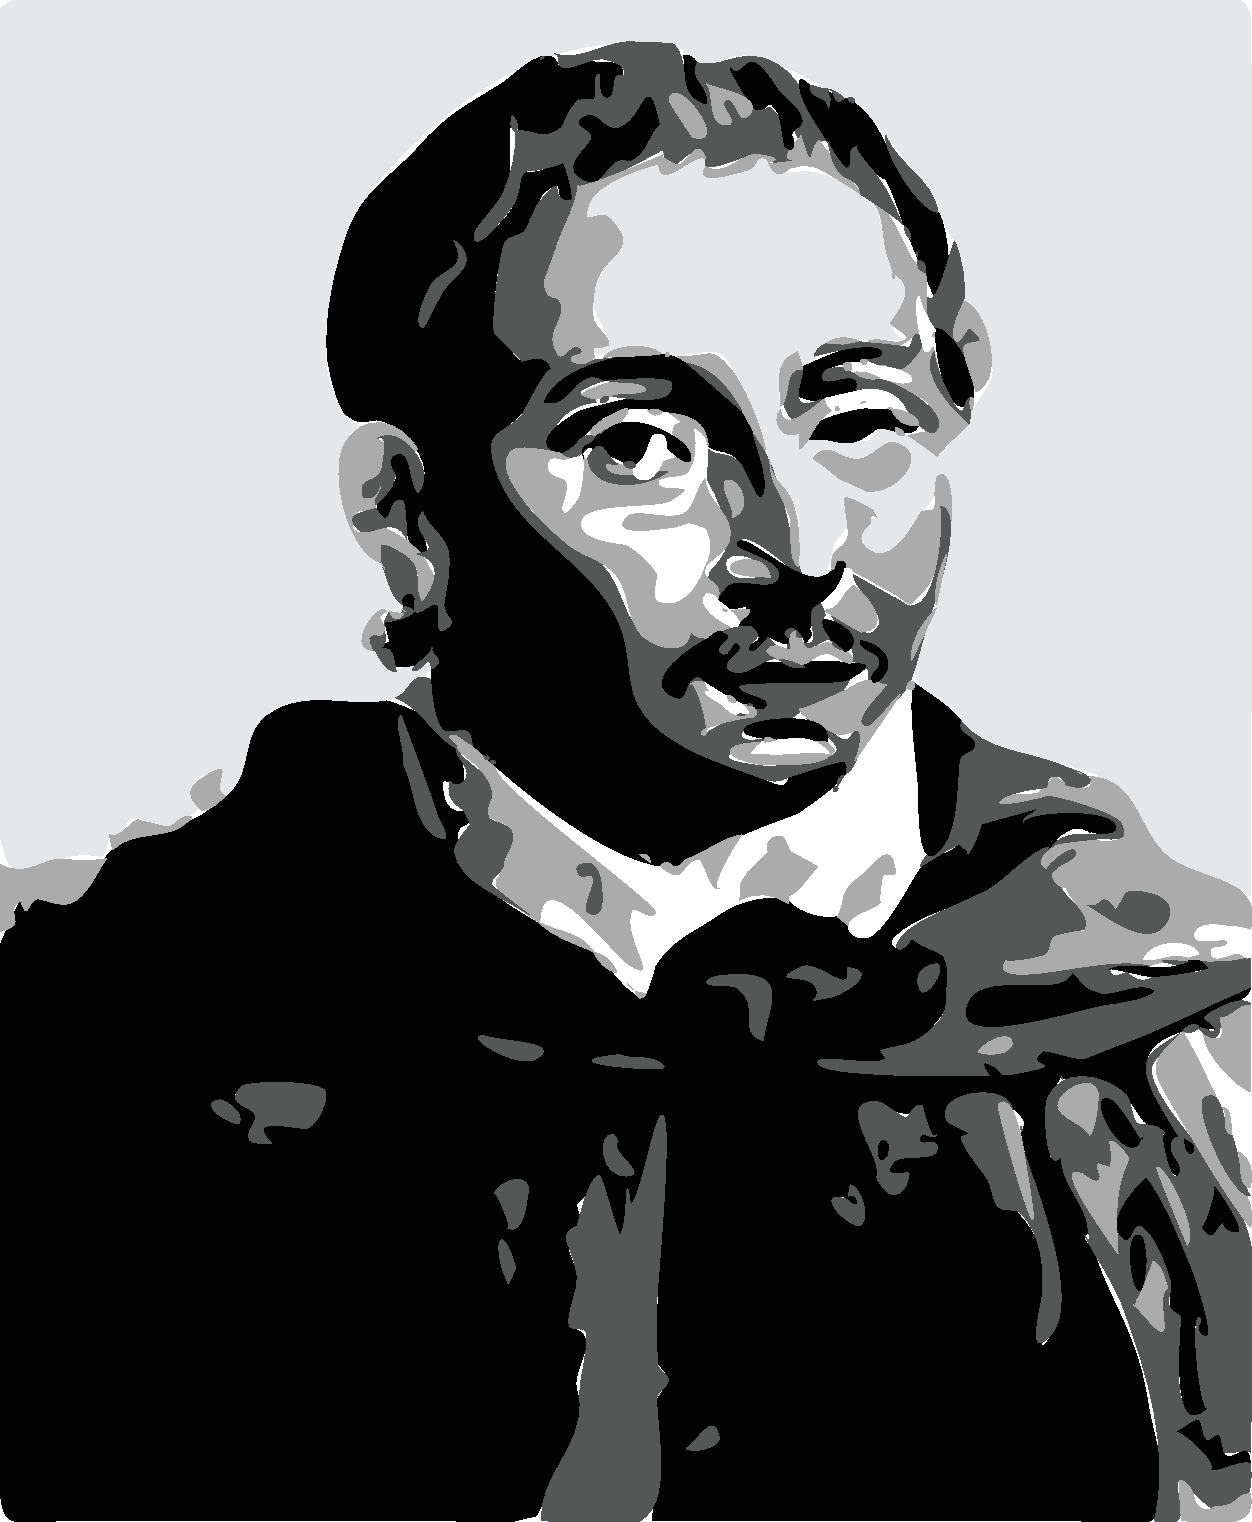
\includegraphics[width=.25\textwidth]{./fotos/calcasdos/Cavalieri.pdf}\\[5pt]
{\small \bfseries Bonaventura Cavalieri}
\end{bio}

\begin{corollary}[Principio de Cavalieri]
  \index{principio!de Cavalieri}Sea $K$ un subconjunto compacto de
  $\mathbb{R}^{n}$, $n>1$. Para cada $t\in \mathbb{R}$, definimos
  \begin{equation*}
    K_{t}:=\left\{y\in \mathbb{R}^{n-1}:(y,t)\in K\right\}.
  \end{equation*}
  Entonces, la función $t\mapsto \vol_{n-1}(K_{t})$
  pertenece a $\mathcal{S}^{\ast }(\mathbb{R})$ y
  \begin{equation*}
    \vol_{n}(K)=\int_{\mathbb{R}}\vol_{n-1}(K_{t})dt.
  \end{equation*}
\end{corollary}

\begin{proof}
  Aplicamos la Proposición~\ref{propfub} con $m=n-1$ a la
  función $1_{K}$. Como $1_{K}^{t}=1_{K_{t}}$ para cada $t\in
  \mathbb{R}$, la función $F$ de la Proposición~\ref{propfub}
  es la función $F(t):=$ vol$_{n-1}(K_{t})$. Dicha proposición
  asegura que $F\in \mathcal{S}^{\ast }(\mathbb{R})$ y que
  \begin{equation*}
    \vol_{n}(K)=\int_{\mathbb{R}^{n}}1_{K}=\int_{\mathbb{R}}F=\int_{\mathbb{R}}\vol_{n-1}(K_{t})dt,
  \end{equation*}
  como afirma el enunciado.
\end{proof}

Usemos el principio de Cavalieri para calcular el volumen de la
bola.

\begin{example}
  \label{volbola}Sea $\bar{B}^{n}(0,r):=\left\{x\in
  \mathbb{R}^{n}:\left\Vert x\right\Vert \leq r\right\}$, $r>0$.
  \index{volumen!de una bola}Entonces
  \begin{equation*}
    \omega_{n}:=\vol_{n}(\bar{B}^{n}(0,1))=
      \begin{cases}
        \frac{1}{k!}\pi^{k} & \text{si $n=2k$,}\\
        \frac{2^{k+1}}{1\cdot 3\cdots (2k+1)}\pi^{k} & \text{si $n=2k+1$,}
      \end{cases}
  \end{equation*}
  y
  \begin{equation*}
    \vol_{n}(\bar{B}^{n}(0,r))=r^{n}\omega_{n}.
  \end{equation*}
\end{example}

\begin{proof}
  Como $\bar{B}^{n}(0,r)=\left\{rx:x\in \bar{B}^{n}(0,1)\right\}$, la
  afirmación
  \begin{equation}
    \vol_{n}(\bar{B}^{n}(0,r))=r^{n}\omega_{n}  \label{r-bola}
  \end{equation}
  es consecuencia de la Proposición~\ref{propvol}. Ahora
  calcularemos $\omega_{n}$.

  Si $n>1$, del principio de Cavalieri y la identidad (\ref{r-bola})
  se sigue que
  \begin{align}
    \omega_{n} &=\int_{-1}^{1}\vol_{n-1}\left( \bar{B}^{n-1}(0,\sqrt{1-t^{2}})\right) dt  \notag \\
    &=\omega_{n-1}\int_{-1}^{1}\left( 1-t^{2}\right)^{\frac{n-1}{2}}dt.
    \label{cav}
  \end{align}
  \begin{figure}[H]
    \centering
    \begin{tikzpicture}[scale=.3]
  \pgfmathsetmacro{\xO}{1}
  \draw[very thin,-latex'] (-6,0)--(6,0);
  \draw[very thin, -latex'] (0,-6)--(0,6);

  \draw[very thin, dashed] (0,0)--(3,4);
  \draw[very thin, dashed] (3,0)--(3,4);

  \draw[thick] (0,0) circle (5);
  \draw[thick] (-3,4)--(3,4);
  \draw[mark=*,mark size=3pt] (-.5,4) node[below] {$t$};
  \draw plot[mark=*,mark size=3pt] coordinates{(0,4)};
\end{tikzpicture}

    % \caption{}\label{fig:12.2}
  \end{figure}
  El cambio de variable $t=\cos x$ nos da
  \begin{equation*}
    c_{n}:=\int_{-1}^{1}\left( 1-t^{2}\right)^{\frac{n-1}{2}}dt=\int_{0}^{\pi
    }\sen^{n}x\text{ }dx.
  \end{equation*}
  Integrando por partes obtenemos que
  \begin{equation*}
    c_{2k}=\pi \prod_{i=1}^{k}\tfrac{2i-1}{2i}\text{\qquad y\qquad }c_{2k+1}=2\prod_{i=1}^{k}\tfrac{2i}{2i+1}.
  \end{equation*}
  Por tanto, $c_{n}c_{n-1}=\frac{2\pi }{n}$, \ lo que implica que
  \begin{equation}
    \omega_{n}=\omega_{n-1}c_{n}=\omega_{n-2}c_{n}c_{n-1}=\tfrac{2\pi }{n}\omega_{n-2}\text{\qquad si }n>2.  \label{cav2}
  \end{equation}
  Como $\omega_{1}:=$ vol$_{1}([-1,1])=2$, de la ecuación
  (\ref{cav}) se sigue que $\omega_{2}=2c_{2}=\pi $. Iterando
  (\ref{cav2}) obtenemos que
  \begin{equation*}
    \omega_{2k}=\frac{1}{k!}\pi^{k}\text{\qquad y\qquad }\omega_{2k+1}=\frac{2^{k+1}}{1\cdot 3\cdots (2k+1)}\pi^{k},
  \end{equation*}
  como afirma el enunciado.
\end{proof}

\section{Funciones Lebesgue-integrables}

Para definir la integral de Lebesgue haremos uso de los siguientes
conceptos.

\begin{definition}
  Para cualquier función $f\colon \mathbb{R}^{n}\rightarrow
  \mathbb{R}\cup \left\{\pm \infty \right\}$ definimos la \textbf{integral
    superior de} $f$ \index{integral!superior}como
  \begin{equation*}
    \int^{\ast }f:=\inf \left\{ \int_{\mathbb{R}^{n}}g:g\in \mathcal{S}_{\ast }(\mathbb{R}^{n}),\text{ }g\geq f\right\} \in \mathbb{R}\cup \left\{\pm \infty \right\},
  \end{equation*}
  y la \textbf{integral inferior de} $f$ \index{integral!inferior}como
  \begin{equation*}
    \int_{\ast }f:=\sup \left\{ \int_{\mathbb{R}^{n}}h:h\in \mathcal{S}^{\ast }(\mathbb{R}^{n}),\text{ }h\leq f\right\} \in \mathbb{R}\cup \left\{\pm \infty \right\}.
  \end{equation*}
\end{definition}

Observa que en ambos casos el conjunto cuyo ínfimo o cuyo supremo
estamos tomando no es vacío, ya que la función constante
$\infty $ pertenece a $\mathcal{S}_{\ast }(\mathbb{R}^{n})$ y la
función constante $-\infty $ pertenece a $\mathcal{S}^{\ast
}(\mathbb{R}^{n})$. Enunciamos a continuación algunas propiedades
sencillas de estas integrales.

\begin{lemma}
  \label{intsupinf}

  \begin{enumerate}
  \item[(a)] Para toda $f\colon \mathbb{R}^{n}\rightarrow \mathbb{R}\cup
    \left\{\pm \infty \right\}$,
    \begin{equation*}
      \int_{\ast }f=-\int^{\ast }\left( -f\right) .
    \end{equation*}

  \item[(b)] Para toda $f\colon \mathbb{R}^{n}\rightarrow \mathbb{R}\cup
    \left\{\pm \infty \right\}$,
    \begin{equation*}
      \int_{\ast }f\leq \int^{\ast }f.
    \end{equation*}

  \item[(c)] Si $f_{1},f_{2}\colon \mathbb{R}^{n}\rightarrow \mathbb{R}\cup
    \left\{\pm \infty \right\}$ cumplen que $f_{1}\leq f_{2}$, entonces
    \begin{equation*}
      \int^{\ast }f_{1}\leq \int^{\ast }f_{2}\text{\qquad y\qquad }\int_{\ast
      }f_{1}\leq \int_{\ast }f_{2}.
    \end{equation*}

  \item[(d)] Si $f\in \mathcal{S}_{\ast }(\mathbb{R}^{n})\cup
    \mathcal{S}^{\ast }(\mathbb{R}^{n})$, entonces
    \begin{equation*}
      \int_{\ast }f=\int^{\ast }f=\int_{\mathbb{R}^{n}}f.
    \end{equation*}

  \item[(e)] Para cualesquiera $f\colon \mathbb{R}^{n}\rightarrow
    \mathbb{R}\cup \left\{\pm \infty \right\}$ y $\lambda \in [0,\infty
    )$,
    \begin{equation*}
      \int^{\ast }\lambda f=\lambda \int^{\ast }f\text{\qquad y\qquad }\int_{\ast
      }\lambda f=\lambda \int_{\ast }f.
    \end{equation*}

  \item[(f)] Para cualesquiera $f_{1},f_{2}\colon \mathbb{R}^{n}\rightarrow
    [0,\infty ]$
    \begin{equation*}
      \int^{\ast }\left( f_{1}+f_{2}\right) \leq \int^{\ast }f_{1}+\int^{\ast
      }f_{2}.
    \end{equation*}
  \end{enumerate}
\end{lemma}

\begin{proof}
  \emph{(a)} es consecuencia inmediata del Lema~\ref{rel}.

  \emph{(b):} \ Basta probar que, si $g\in \mathcal{S}_{\ast
  }(\mathbb{R}^{n})$, $h\in \mathcal{S}^{\ast }(\mathbb{R}^{n})$ y
  $h\leq g$, entonces
  \begin{equation*}
    \int_{\mathbb{R}^{n}}h\leq \int_{\mathbb{R}^{n}}g.
  \end{equation*}
  Del Corolario~\ref{correl} y la monotonía de la integral
  (Proposición~\ref{linmonsc}) se sigue que
  \begin{equation*}
    \int_{\mathbb{R}^{n}}g-\int_{\mathbb{R}^{n}}h=\int_{\mathbb{R}^{n}}\left(
      g-h\right) \geq 0.
  \end{equation*}
  Esta es la desigualdad deseada.

  \emph{(c)} es consecuencia inmediata de la definición.

  \emph{(d):} \ Sea $f\in \mathcal{S}_{\ast }(\mathbb{R}^{n})$. La
  igualdad
  \begin{equation*}
    \int^{\ast }f=\int_{\mathbb{R}^{n}}f
  \end{equation*}
  es consecuencia inmediata de la definición de la integral
  superior. Sean $f_{k}\in \mathcal{C}_{c}^{0}(\mathbb{R}^{n})$, tales
  que $f_{k}\leq f_{k+1}$ y $\sup_{k\in \mathbb{N}}f_{k}=f$. En
  particular, $f_{k}\in \mathcal{S}^{\ast }(\mathbb{R}^{n})$ y
  $f_{k}\leq f$. De la definición de integral inferior y la
  afirmación \emph{(b)} obtenemos
  \begin{equation*}
    \int_{\mathbb{R}^{n}}f=\lim_{k\rightarrow \infty }\int_{\mathbb{R}^{n}}f_{k}\leq \int_{\ast }f\leq \int^{\ast }f=\int_{\mathbb{R}^{n}}f,
  \end{equation*}
{\abovedisplayskip=7pt%
\belowdisplayskip=7pt%
  es decir,
  \begin{equation*}
    \int_{\ast }f=\int^{\ast }f=\int_{\mathbb{R}^{n}}f\text{\qquad }\forall f\in 
    \mathcal{S}_{\ast }(\mathbb{R}^{n}).
  \end{equation*}
  Si $f\in \mathcal{S}^{\ast }(\mathbb{R}^{n})$, las identidades
  correspondientes se siguen de éstas utilizando la afirmación
  \emph{(a)}\ y el Lema~\ref{rel}.

  \emph{(e):} \ Si $\lambda =0$ el resultado es obvio. Supongamos que
  $\lambda >0$. Para toda $g\in \mathcal{S}_{\ast }(\mathbb{R}^{n})$
  tal que $g\geq \lambda f$, se tiene que $\lambda^{-1}g\in
  \mathcal{S}_{\ast }(\mathbb{R}^{n})$ y $\lambda^{-1}g\geq f$.
  Usando la Proposición~\ref{linmonsc} obtenemos
  \begin{equation*}
    \lambda \int^{\ast }f\leq \lambda \int_{\mathbb{R}^{n}}\lambda^{-1}g=\int_{\mathbb{R}^{n}}g.
  \end{equation*}
  Se tiene entonces que
  \begin{equation*}
    \lambda \int^{\ast }f\leq \int^{\ast }\lambda f.
  \end{equation*}
  Reemplazando $f$ por $\lambda f$ y $\lambda $ por $\lambda^{-1}$ en
  la desigualdad anterior obtenemos
  \begin{equation*}
    \lambda^{-1}\int^{\ast }\lambda f\leq \int^{\ast }f,
  \end{equation*}
  es decir,
  \begin{equation*}
    \int^{\ast }\lambda f\leq \lambda \int^{\ast }f.
  \end{equation*}
  Esto prueba la igualdad para la integral superior. La igualdad para
  la integral inferior se obtiene aplicando la afirmación
  \emph{(a)}.

  \emph{(f):} \ Si $\int^{\ast }f_{1}=\infty $ o $\int^{\ast
  }f_{2}=\infty $ la desigualdad deseada se cumple
  trivialmente. Supongamos que $\int^{\ast }f_{1}<\infty $ y
  $\int^{\ast }f_{2}<\infty $. Sea $\varepsilon >0$ y sean
  $g_{1},g_{2}\in \mathcal{S}_{\ast }(\mathbb{R}^{n})$ tales que
  $g_{1}\geq f_{1}$, $g_{2}\geq f_{2}$,
  \begin{equation*}
    \int_{\mathbb{R}^{n}}g_{1}\leq \biggl( \int^{\ast }f_{1}\biggr) +\frac{\varepsilon }{2}\text{\qquad y\qquad }\int_{\mathbb{R}^{n}}g_{2}\leq \left(
      \int^{\ast }f_{2}\right) +\frac{\varepsilon }{2}.
  \end{equation*}
  Entonces, $g_{1}+g_{2}\in \mathcal{S}_{\ast }(\mathbb{R}^{n})$,
  $g_{1}+g_{2}\geq f_{1}+f_{2}$ y, sumando las desigualdades
  anteriores, obtenemos
  \begin{equation*}
    \int^{\ast }\left( f_{1}+f_{2}\right) \leq \int_{\mathbb{R}^{n}}\left(
      g_{1}+g_{2}\right) \leq \biggl( \int^{\ast }f_{1}+\int^{\ast }f_{2}\biggr)
    +\varepsilon .
  \end{equation*}
  En consecuencia,
  \begin{equation*}
    \int^{\ast }\left( f_{1}+f_{2}\right) \leq \int^{\ast }f_{1}+\int^{\ast
    }f_{2},
  \end{equation*}
  como se afirma en \emph{(f).}}%
\end{proof}
{\abovedisplayskip=7pt
\belowdisplayskip=7pt
\begin{definition}
  \label{defintleb}Una función $f\colon \mathbb{R}^{n}\rightarrow
  \mathbb{R}\cup \left\{\pm \infty \right\}$ es \textbf{(Lebesgue-) integrable}
  \index{función!integrable}si
  \begin{equation*}
    -\infty <\int_{\ast }f=\int^{\ast }f<\infty .
  \end{equation*}
  En este caso, la \textbf{integral (de Lebesgue}\footnote{Henri
    Léon Lebesgue (1875-1941) nació en Beauvais, Oise,
    Francia.  Estudió en la Sorbonne de Paris, donde fue
    alumno de Émile Borel. Introdujo su teoría de
    integración en 1902 en su tesis de doctorado titulada
    \textit{Integral, longitud y área}.}\textbf{) de} $f$
  \index{integral!de Lebesgue}se define como
  \begin{equation*}
    \int_{\mathbb{R}^{n}}f:=\int_{\ast }f=\int^{\ast }f\text{ \ }\in \mathbb{R}.
  \end{equation*}
\end{definition}}%
\begin{bio}[htb]
\centering
%
\includegraphics[width=.3\textwidth]{./fotos/calcasdos/Frechet.png}\\[5pt]
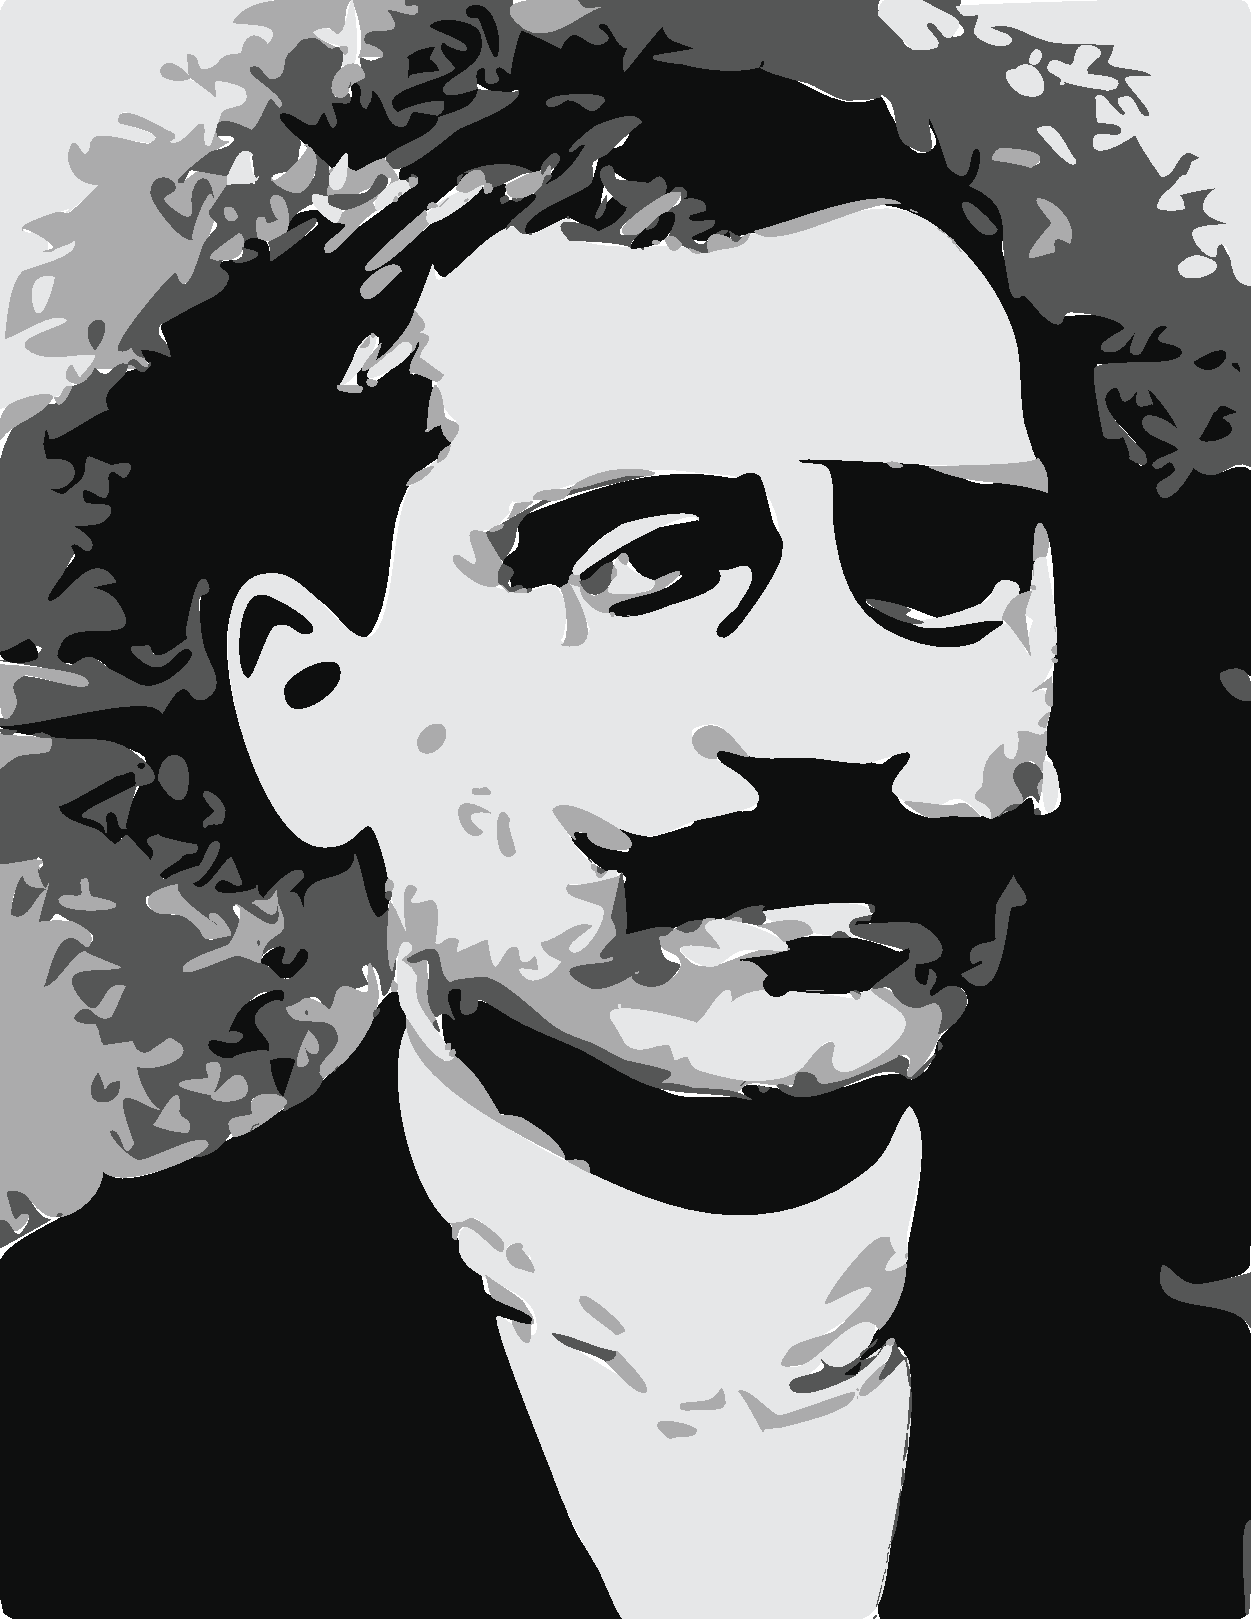
\includegraphics[width=.3\textwidth]{./fotos/calcasdos/Lebesgue.pdf}\\[4pt]
{\small \bfseries Henri Lebesgue}
\end{bio}

\begin{remark}
  \label{obsintleb}Del \emph{Lema~\ref{intsupinf}} se infiere lo
  siguiente:

  \begin{enumerate}
{\abovedisplayskip=7pt
\belowdisplayskip=7pt
  \item[(a)] Si $f\in \mathcal{S}_{\ast }(\mathbb{R}^{n})\cup
    \mathcal{S}^{\ast }(\mathbb{R}^{n})$, entonces $f$ es
    Lebesgue-integrable si y sólo si la integral definida en la
    \emph{Sección~\ref{secintsc}} cumple que
    \begin{equation*}
      -\infty <\int_{\mathbb{R}^{n}}f<\infty .
    \end{equation*}
    En este caso, la integral de Lebesgue de $f$ coincide con dicha
    integral.}%

  \item[(b)] En particular, si $f\in
    \mathcal{C}_{c}^{0}(\mathbb{R}^{n})$, entonces $f$ es
    Lebesgue-integrable y la integral de Lebesgue de $f$ coincide con
    la de la \emph{Definición~\ref{defintsopcomp}}.
  \end{enumerate}
\end{remark}

La Definición~\ref{defintleb}\ se puede reformular como sigue.

\begin{lemma}
  \label{ref}$f\colon \mathbb{R}^{n}\rightarrow \mathbb{R}\cup \left\{\pm \infty
  \right\}$ es Lebesgue-integrable si y sólo si para cada $\varepsilon
  >0$ existen $h\in \mathcal{S}^{\ast }(\mathbb{R}^{n})$ y $g\in
  \mathcal{S}_{\ast }(\mathbb{R}^{n})$ tales que $h\leq f\leq g$,
  \begin{equation*}
    -\infty <\int_{\mathbb{R}^{n}}h\text{,\qquad }\int_{\mathbb{R}^{n}}g<\infty 
    \text{\qquad y\qquad }0\leq \int_{\mathbb{R}^{n}}g-\int_{\mathbb{R}^{n}}h<\varepsilon .
  \end{equation*}
\end{lemma}

\begin{proof}
  $\Rightarrow )$: \ Si $f\colon \mathbb{R}^{n}\rightarrow \mathbb{R}\cup
  \left\{\pm \infty \right\}$ es Lebesgue-integrable entonces, como su integral
  superior y su integral inferior son finitas, para cada $\varepsilon
  >0$, existen $h\in \mathcal{S}^{\ast }(\mathbb{R}^{n})$ y $g\in
  \mathcal{S}_{\ast }(\mathbb{R}^{n})$ tales que $h\leq f\leq g$ y
  \begin{equation*}
    \int_{\mathbb{R}^{n}}g\leq \int^{\ast }f+\frac{\varepsilon }{2}<\infty \text{\qquad y\qquad }-\infty <\int_{\ast }f-\frac{\varepsilon }{2}<\int_{\mathbb{R}^{n}}h.
  \end{equation*}
  Dado que la integral superior y la integral inferior de $f$
  coinciden, concluimos que
  \begin{equation*}
    0=\int^{\ast }f-\int_{\ast }f\leq \int_{\mathbb{R}^{n}}g-\int_{\mathbb{R}^{n}}h<\int^{\ast }f-\int_{\ast }f+\varepsilon =\varepsilon .
  \end{equation*}
  $\Leftarrow )$: \ Inversamente, si para cada $\varepsilon >0$
  existen $h\in \mathcal{S}^{\ast }(\mathbb{R}^{n})$ y $g\in
  \mathcal{S}_{\ast }(\mathbb{R}^{n})$ tales que $h\leq f\leq g$,
  \begin{equation*}
    -\infty <\int_{\mathbb{R}^{n}}h\text{,\qquad }\int_{\mathbb{R}^{n}}g<\infty 
    \text{\qquad y\qquad }\int_{\mathbb{R}^{n}}g-\int_{\mathbb{R}^{n}}h<\varepsilon ,
  \end{equation*}
  entonces
  \begin{equation*}
    -\infty <\int_{\mathbb{R}^{n}}h\leq \int_{\ast }f\leq \int^{\ast }f\leq
    \int_{\mathbb{R}^{n}}g<\infty
  \end{equation*}
  y, en consecuencia,
  \begin{equation*}
    0\leq \int^{\ast }f-\int_{\ast }f\leq \int_{\mathbb{R}^{n}}g-\int_{\mathbb{R}^{n}}h<\varepsilon
  \end{equation*}
  para todo $\varepsilon >0$. Esto prueba que $f$ es
  Lebesgue-integrable.
\end{proof}

El siguiente resultado proporciona una caracterización muy
útil de las funciones Lebesgue-integrables y permite expresar a su
integral como el límite de integrales de funciones en
$\mathcal{C}_{c}^{0}(\mathbb{R}^{n}) $.

Dada $f\colon \mathbb{R}^{n}\rightarrow \mathbb{R}\cup \left\{\pm \infty \right\}$,
definimos $\left\vert f\right\vert \colon \mathbb{R}^{n}\rightarrow
\mathbb{R}\cup \left\{\infty \right\}$ como
\begin{equation*}
  \left\vert f\right\vert (x):=\left\vert f(x)\right\vert ,
\end{equation*}
donde $\left\vert \pm \infty \right\vert :=\infty $.

\begin{proposition}
  \label{caractint}Sea $f\colon \mathbb{R}^{n}\rightarrow \mathbb{R}\cup
  \left\{\pm \infty \right\}$. Entonces $f$ es Lebesgue-integrable si y sólo
  si existe una sucesión $(\varphi_{k})$ en
  $\mathcal{C}_{c}^{0}(\mathbb{R}^{n})$ tal que
  \begin{equation*}
    \lim_{k\rightarrow \infty }\int^{\ast }\left\vert f-\varphi_{k}\right\vert
    =0.
  \end{equation*}
  En ese caso, se cumple que
  \begin{equation*}
    \int_{\mathbb{R}^{n}}f=\lim_{k\rightarrow \infty }\int_{\mathbb{R}^{n}}\varphi_{k}.
  \end{equation*}
\end{proposition}

\begin{proof}
  $\Rightarrow )$:\emph{\ \ }Supongamos que $f$ es
  Lebesgue-integrable. Basta probar que, para cada $\varepsilon >0$,
  existe $\varphi \in \mathcal{C}_{c}^{0}(\mathbb{R}^{n})$ tal que
  \begin{equation}
    \int^{\ast }\left\vert f-\varphi \right\vert <\varepsilon .  \label{af1}
  \end{equation}
  Por el Lema~\ref{ref} y el Corolario~\ref{correl}, existen $g\in
  \mathcal{S}_{\ast }(\mathbb{R}^{n})$ y $h\in \mathcal{S}^{\ast
  }(\mathbb{R}^{n})$ tales que $h\leq f\leq g$ y
  \begin{equation*}
    -\infty <\int_{\mathbb{R}^{n}}h,\text{\qquad }\int_{\mathbb{R}^{n}}g<\infty 
    \text{\qquad y\qquad }\int_{\mathbb{R}^{n}}(g-h)<\frac{\varepsilon }{2}.
  \end{equation*}
  Por otra parte, de la definición de la integral para funciones
  en $\mathcal{S}_{\ast }(\mathbb{R}^{n})$ se sigue que existe
  $\varphi \in \mathcal{C}_{c}^{0}(\mathbb{R}^{n})$ tal que $\varphi
  \leq g$ y
  \begin{equation*}
    \int_{\mathbb{R}^{n}}\left( g-\varphi \right) <\frac{\varepsilon }{2}.
  \end{equation*}
  Como
  \begin{equation*}
    \left\vert f-\varphi \right\vert (x)=
      \begin{cases}
        f(x)-\varphi (x)\leq g(x)-\varphi (x) &\text{si $f(x)\geq \varphi (x)$,}
        \\ 
        \varphi (x)-f(x)\leq g(x)-h(x) &\text{si $f(x)\leq \varphi (x)$,}
      \end{cases}
  \end{equation*}
  se tiene que
  \begin{equation*}
    \left\vert f-\varphi \right\vert \leq (g-h)+(g-\varphi )\in \mathcal{S}_{\ast }(\mathbb{R}^{n}).
  \end{equation*}
  Usando el Lema~\ref{intsupinf} y la Proposición~\ref{linmonsc},
  concluimos que
  \begin{equation*}
    \int^{\ast }\left\vert f-\varphi \right\vert \leq \int_{\mathbb{R}^{n}}\left[
      (g-h)+(g-\varphi )\right] =\int_{\mathbb{R}^{n}}(g-h)+\int_{\mathbb{R}^{n}}(g-\varphi )<\varepsilon .
  \end{equation*}
  Esto prueba la afirmación (\ref{af1}).

  $\Leftarrow )$: \ Supongamos que existe una sucesión $(\varphi
 _{k})$ en $\mathcal{C}_{c}^{0}(\mathbb{R}^{n})$ tal que
  \begin{equation*}
    \lim_{k\rightarrow \infty }\int^{\ast }\left\vert f-\varphi_{k}\right\vert
    =0.
  \end{equation*}
  Sea $\varepsilon >0$ y sea $k_{0}\in \mathbb{N}$ tal que
  \begin{equation*}
    \int^{\ast }\left\vert f-\varphi_{k}\right\vert <\frac{\varepsilon }{2}\text{\qquad si \ }k\geq k_{0}.
  \end{equation*}
  Entonces, por definición de la integral superior, para cada
  $k\geq k_{0}$\ existe $g_{k}\in \mathcal{S}_{\ast }(\mathbb{R}^{n})$
  tal que $g_{k}\geq \left\vert f-\varphi_{k}\right\vert $ y
  \begin{equation*}
    \int^{\ast }\left\vert f-\varphi_{k}\right\vert \leq \int_{\mathbb{R}^{n}}g_{k}<\frac{\varepsilon }{2}.
  \end{equation*}
  Por tanto,
  $g_{k}+\varphi_{k}\in \mathcal{S}_{\ast }(\mathbb{R}^{n})$,
  $-g_{k}+\varphi_{k}\in \mathcal{S}^{\ast }(\mathbb{R}^{n})$ y
  $-g_{k}+\varphi_{k}\leq f\leq g_{k}+\varphi _{k}$. Aplicando el
  Lema~\ref{intsupinf} y la Proposición~\ref{linmonsc} obtenemos que
  \begin{align}
    -\infty &<-\frac{\varepsilon }{2}+\int_{\mathbb{R}^{n}}\varphi_{k}<-\int_{\mathbb{R}^{n}}g_{k}+\int_{\mathbb{R}^{n}}\varphi_{k}=\int_{\ast
    }(-g_{k}+\varphi_{k})\leq \int_{\ast }f  \notag \\
    &\leq \int^{\ast }f\leq \int^{\ast }(g_{k}+\varphi_{k})=\int_{\mathbb{R}^{n}}g_{k}+\int_{\mathbb{R}^{n}}\varphi_{k}<\frac{\varepsilon }{2}+\int_{\mathbb{R}^{n}}\varphi_{k}<\infty .  \label{fin}
  \end{align}
  En consecuencia,
  \begin{equation*}
    0\leq \int^{\ast }f-\int_{\ast }f\leq \varepsilon .
  \end{equation*}
  Concluimos que
  \begin{equation*}
    -\infty <\int_{\ast }f=\int^{\ast }f<\infty ,
  \end{equation*}
  es decir, $f$ es Lebesgue-integrable.

  Finalmente, se sigue de (\ref{fin}) que
  \begin{equation*}
    \left\vert \int_{\mathbb{R}^{n}}f-\int_{\mathbb{R}^{n}}\varphi
     _{k}\right\vert <\frac{\varepsilon }{2}\text{\qquad }\forall k\geq k_{0}.
  \end{equation*}
  Esto prueba que
  \begin{equation*}
    \int_{\mathbb{R}^{n}}f=\lim_{k\rightarrow \infty }\int_{\mathbb{R}^{n}}\varphi_{k}
  \end{equation*}
  como afirma el enunciado.
\end{proof}

\section{Propiedades básicas de la integral de Lebesgue}

Usaremos la Proposición~\ref{caractint} para probar algunas
propiedades fundamentales de la integral de Lebesgue. Empecemos
observando lo siguiente.
\begin{proposition}
  \label{valabsint}

  \begin{enumerate}
  \item[(a)] Si $f\colon \mathbb{R}^{n}\rightarrow \mathbb{R}\cup \left\{\pm
    \infty \right\}$ es Lebesgue-integrable, entonces $-f$ es
    Lebesgue-integrable y
    \begin{equation*}
      \int_{\mathbb{R}^{n}}\left( -f\right) =-\int_{\mathbb{R}^{n}}f.
    \end{equation*}

  \item[(b)] Si $f\colon \mathbb{R}^{n}\rightarrow \mathbb{R}\cup \left\{\pm
    \infty \right\}$ es Lebesgue-integrable, entonces $\left\vert
      f\right\vert $ es Lebesgue-integrable y
    \begin{equation*}
      \left\vert \int_{\mathbb{R}^{n}}f\right\vert \leq \int_{\mathbb{R}^{n}}\left\vert f\right\vert .
    \end{equation*}
  \end{enumerate}
\end{proposition}

\begin{proof}
  \emph{(a):} \ Si $f\colon \mathbb{R}^{n}\rightarrow \mathbb{R}\cup \left\{\pm
  \infty \right\}$ es Lebesgue-integrable, usando el Lema~\ref{intsupinf}
  obtenemos que
  \begin{equation*}
    \int^{\ast }\left( -f\right) =-\int_{\ast }f=-\int^{\ast }f=\int_{\ast
    }\left( -f\right) .
  \end{equation*}
  Esto demuestra la afirmación \emph{(a)}.

  {\abovedisplayskip=7pt%
    \belowdisplayskip=7pt%
  \emph{(b):} \ La Proposición~\ref{caractint} asegura que existe
  una sucesión $(\varphi_{k})$ en
  $\mathcal{C}_{c}^{0}(\mathbb{R}^{n})$ tal que
  \begin{equation*}
    \lim_{k\rightarrow \infty }\int^{\ast }\left\vert f-\varphi_{k}\right\vert
    =0.
  \end{equation*}
  Observa que $0\leq \left\vert \left\vert f\right\vert -\left\vert
      \varphi_{k}\right\vert \right\vert \leq \left\vert f-\varphi
   _{k}\right\vert $. Así que, por la monotonía de la
  integral superior,
  \begin{equation*}
    0\leq \lim_{k\rightarrow \infty }\int^{\ast }\left\vert \left\vert
        f\right\vert -\left\vert \varphi_{k}\right\vert \right\vert \leq
    \lim_{k\rightarrow \infty }\int^{\ast }\left\vert f-\varphi_{k}\right\vert
    =0.
  \end{equation*}
  La Proposición~\ref{caractint} asegura entonces que
  $\left\vert f\right\vert $ es Lebesgue-integrable y, junto con el
  Ejercicio~\ref{valabs}, asegura además que
  \begin{equation*}
    \int_{\mathbb{R}^{n}}\left\vert f\right\vert =\lim_{k\rightarrow \infty
    }\int_{\mathbb{R}^{n}}\left\vert \varphi_{k}\right\vert \geq
    \lim_{k\rightarrow \infty }\left\vert \int_{\mathbb{R}^{n}}\varphi
     _{k}\right\vert =\left\vert \int_{\mathbb{R}^{n}}f\right\vert ,
  \end{equation*}
  como afirma el enunciado.}%
\end{proof}
{\abovedisplayskip=7pt
\belowdisplayskip=7pt

Veremos más adelante que una función Lebesgue-integrable
$f\colon \mathbb{R}^{n}\rightarrow \mathbb{R}\cup \left\{\pm \infty \right\}$ sólo
toma los valores $\pm \infty $ en un conjunto muy pequeño que no
afecta el valor de la integral (ver Proposición
\ref{funcfinita}). Por ello consideraremos en el resto de esta
sección únicamente funciones que toman valores reales.

Denotemos por
\begin{equation*}
  \mathfrak{L}(\mathbb{R}^{n}):=\left\{f\colon \mathbb{R}^{n}\rightarrow \mathbb{R}:f\text{ es Lebesgue-integrable}\right\}.
\end{equation*}
El siguiente resultado afirma que $\mathfrak{L}(\mathbb{R}^{n})$ es un
espacio vectorial y que la integral es una función lineal y
monótona.

\begin{theorem}[Linealidad y monotonía]
  \label{linmon}

  \begin{enumerate}
  \item[(a)] \index{linealidad!de la integral}Si $f_{1},f_{2}\in
    \mathfrak{L}(\mathbb{R}^{n})$ y $\lambda_{1},\lambda_{2}\in
    \mathbb{R}$, entonces $\lambda_{1}f_{1}+\lambda_{2}f_{2}\in
    \mathfrak{L}(\mathbb{R}^{n})$ y
    \begin{equation*}
      \int_{\mathbb{R}^{n}}\left( \lambda_{1}f_{1}+\lambda_{2}f_{2}\right)
      =\lambda_{1}\int_{\mathbb{R}^{n}}f_{1}+\lambda_{2}\int_{\mathbb{R}^{n}}f_{2}.
    \end{equation*}

  \item[(b)] \index{monotonia!de la integral}Si $f,g\in
    \mathfrak{L}(\mathbb{R}^{n})$ y $f\leq g$, entonces
    \begin{equation*}
      \int_{\mathbb{R}^{n}}f\leq \int_{\mathbb{R}^{n}}g.
    \end{equation*}
  \end{enumerate}
\end{theorem}}%

\begin{proof}
{\abovedisplayskip=7pt
\belowdisplayskip=7pt
  \emph{(a): \ }Sean $f_{1},f_{2}\in \mathfrak{L}(\mathbb{R}^{n})$ y
  $\lambda_{1},\lambda_{2}\in \mathbb{R}$. La
  Proposición~\ref{caractint}\ asegura que, para cada
  $k\in \mathbb{N}$, existen
  $\varphi_{1,k},\varphi_{2,k}\in \mathcal{C}_{c}^{0}(\mathbb{R}^{n})$
  tales que
  \begin{equation*}
    \lim_{k\rightarrow \infty }\int^{\ast }\left\vert f_{i}-\varphi
     _{i,k}\right\vert =0\text{\qquad para }i=1,2.
  \end{equation*}}%
  De las afirmaciones \emph{(c)}, \emph{(e)} y \emph{(f)} del
  Lema~\ref{intsupinf} se sigue que
  \begin{align*}
    0&\leq \int^{\ast }\left\vert \lambda_{1}f_{1}+\lambda_{2}f_{2}-\lambda
     _{1}\varphi_{1,k}-\lambda_{2}\varphi_{2,k}\right\vert\\ 
    &\leq \left\vert
      \lambda_{1}\right\vert \int^{\ast }\left\vert f_{1}-\varphi
     _{1,k}\right\vert +\left\vert \lambda_{2}\right\vert \int^{\ast }\left\vert
      f_{2}-\varphi_{2,k}\right\vert .
  \end{align*}
  En consecuencia,
  \begin{equation*}
    \lim_{k\rightarrow \infty }\int^{\ast }\left\vert (\lambda_{1}f_{1}+\lambda
     _{2}f_{2})-(\lambda_{1}\varphi_{1,k}+\lambda_{2}\varphi
     _{2,k})\right\vert =0.
  \end{equation*}
  La Proposición~\ref{caractint} asegura entonces que $\lambda
 _{1}f_{1}+\lambda_{2}f_{2}\in \mathfrak{L}(\mathbb{R}^{n})$ y
  \begin{align*}
    \int_{\mathbb{R}^{n}}\left( \lambda_{1}f_{1}+\lambda_{2}f_{2}\right)
    &=\lim_{k\rightarrow \infty }\int_{\mathbb{R}^{n}}\left( \lambda
     _{1}\varphi_{1,k}+\lambda_{2}\varphi_{2,k}\right) \\
    &=\lim_{k\rightarrow \infty }\lambda_{1}\int_{\mathbb{R}^{n}}\varphi
   _{1,k}+\lim_{k\rightarrow \infty }\lambda_{2}\int_{\mathbb{R}^{n}}\varphi
   _{2,k}\\
    &=\lambda_{1}\int_{\mathbb{R}^{n}}f_{1}+\lambda_{2}\int_{\mathbb{R}^{n}}f_{2}.
  \end{align*}
  Esto demuestra la linealidad.

  \emph{(b): \ }La monotonía es consecuencia inmediata de la
  Definición~\ref{defintleb}\ y la afirmación \emph{(c)} del
  Lema~\ref{intsupinf}.
\end{proof}

Ahora probaremos el teorema de cambio de variable para isometrías
afines.  El teorema de cambio de variable para difeomorfismos es
más delicado. Lo demostraremos en el siguiente capítulo.

\begin{theorem}[Cambio lineal de variable]
  \label{cvlinleb}\index{teorema!de cambio de variable}Sean $A\in
  GL(n,\mathbb{R})$ y $\zeta \in \mathbb{R}^{n}$. Si $f\in
  \mathfrak{L}(\mathbb{R}^{n})$ entonces la función $x\mapsto
  f(Ax+\zeta )$ pertenece a $\mathfrak{L}(\mathbb{R}^{n})$ y se cumple
  que
  \begin{equation*}
    \int_{\mathbb{R}^{n}}f(Ax+\zeta )\left\vert \det A\right\vert dx=\int_{\mathbb{R}^{n}}f(y)dy.
  \end{equation*}
\end{theorem}

\begin{proof}
  Sean $h\in \mathcal{S}^{\ast }(\mathbb{R}^{n})$ y $g\in
  \mathcal{S}_{\ast }(\mathbb{R}^{n})$ tales que $h\leq f\leq g$.
  Denotemos por $F(x):=Ax+\zeta $. Por la Proposición~\ref{cvsc},
  $\left( h\circ F\right) \left\vert \det A\right\vert \in
  \mathcal{S}^{\ast }(\mathbb{R}^{n})$, $\left( g\circ F\right)
  \left\vert \det A\right\vert \in \mathcal{S}_{\ast
  }(\mathbb{R}^{n})$,
  \begin{equation*}
    \int_{\mathbb{R}^{n}}\left( h\circ F\right) \left\vert \det A\right\vert
    =\int_{\mathbb{R}^{n}}h\text{\qquad y\qquad }\int_{\mathbb{R}^{n}}\left( g\circ F\right) \left\vert
      \det A\right\vert =\int_{\mathbb{R}^{n}}g.
  \end{equation*}
  Por tanto,
  \begin{align*}
    \int_{\mathbb{R}^{n}}f &=\inf \left\{ \int_{\mathbb{R}^{n}}\left( g\circ
        F\right) \left\vert \det A\right\vert :g\in \mathcal{S}_{\ast }(\mathbb{R}^{n}),\text{ }g\geq f\right\} \\
    &=\sup \left\{ \int_{\mathbb{R}^{n}}\left( h\circ F\right) \left\vert \det
        A\right\vert :h\in \mathcal{S}^{\ast }(\mathbb{R}^{n}),\text{ }h\leq
      f\right\} .
  \end{align*}
  Por otra parte, como $\left( h\circ F\right) \left\vert \det
    A\right\vert \leq \left( f\circ F\right) \left\vert \det
    A\right\vert \leq \left( g\circ F\right) \left\vert \det
    A\right\vert $ se tiene que
  \begin{gather*}
    \int_{\mathbb{R}^{n}}\left( h\circ F\right) \left\vert \det A\right\vert
    \leq \int_{\ast }\left( f\circ F\right) \left\vert \det
      A\right\vert, \\
    \int^{\ast }\left( f\circ F\right) \left\vert \det
      A\right\vert \leq \int_{\mathbb{R}^{n}}\left( g\circ F\right) \left\vert
      \det A\right\vert .
  \end{gather*}
  En consecuencia,
  \begin{equation*}
    \int^{\ast }\left( f\circ F\right) \left\vert \det A\right\vert \leq \int_{\mathbb{R}^{n}}f\leq \int_{\ast }\left( f\circ F\right) \left\vert \det
      A\right\vert .
  \end{equation*}
  Del Lema~\ref{intsupinf} se sigue la igualdad y, por tanto, la
  integrabilidad de $f\circ F$ y la identidad deseada.
\end{proof}

Si $1\leq m<n$,\: $g\colon \mathbb{R}^{m}\rightarrow \mathbb{R}$ y
$h\colon \mathbb{R}^{n-m}\rightarrow \mathbb{R}$, definimos $g\odot
h\colon \mathbb{R}^{n}\rightarrow \mathbb{R}$ como
\begin{equation}
  \left( g\odot h\right) (y,z):=g(y)h(z),\text{\qquad donde \ }(y,z)\in 
  \mathbb{R}^{m}\times \mathbb{R}^{n-m}\equiv \mathbb{R}^{n}.
  \label{prodcomple}
\end{equation}
Se tiene el siguiente resultado.

\begin{proposition}
  \label{prodtens}Si $f_{1}\in \mathfrak{L}(\mathbb{R}^{m})$ y
  $f_{2}\in \mathfrak{L}(\mathbb{R}^{n-m})$, $1\leq m<n$, entonces
  $f_{1}\odot f_{2}\in \mathfrak{L}(\mathbb{R}^{n})$ y
  \begin{equation*}
    \int_{\mathbb{R}^{n}}\left( f_{1}\odot f_{2}\right) =\biggl( \int_{\mathbb{R}^{m}}f_{1}\biggr) \biggl( \int_{\mathbb{R}^{n-m}}f_{2}\biggr) .
  \end{equation*}
\end{proposition}

\begin{proof}
  Por la Proposición~\ref{valabsint}, si $f_{1}\in
  \mathfrak{L}(\mathbb{R}^{m})$ y $f_{2}\in
  \mathfrak{L}(\mathbb{R}^{n-m})$ entonces $\left\vert
    f_{1}\right\vert \in \mathfrak{L}(\mathbb{R}^{m})$ y $\left\vert
    f_{2}\right\vert \in \mathfrak{L}(\mathbb{R}^{n-m})$. Por tanto,
  existe $M\in \mathbb{R}$ tal que
  \begin{equation*}
    \max \left\{ \int_{\mathbb{R}^{m}}\left\vert f_{1}\right\vert ,\text{ }\int_{\mathbb{R}^{n-m}}\left\vert f_{2}\right\vert \right\} <M.
  \end{equation*}
  Elegimos $\tilde{g}\in \mathcal{S}_{\ast }(\mathbb{R}^{m})$ tal que
  $\tilde{g}\geq \left\vert f_{1}\right\vert $ y
  \begin{equation}
    \int_{\mathbb{R}^{m}}\tilde{g}<M.  \label{prod1}
  \end{equation}
{\abovedisplayskip=9.5pt%
\belowdisplayskip=9pt%
  Por otra parte, la Proposición~\ref{caractint} asegura que
  existen $\varphi_{1,k}\in \mathcal{C}_{c}^{0}(\mathbb{R}^{m})$,
  $\varphi_{2,k}\in \mathcal{C}_{c}^{0}(\mathbb{R}^{n-m})$ tales que
  \begin{equation*}
    \lim_{k\rightarrow \infty }\int_{\mathbb{R}^{m}}\left\vert f_{1}-\varphi
     _{1,k}\right\vert =0\text{\qquad y\qquad }\lim_{k\rightarrow \infty }\int_{\mathbb{R}^{n-m}}\left\vert f_{2}-\varphi_{2,k}\right\vert =0.
  \end{equation*}
  Sea $\varepsilon >0$. Entonces existe $k_{0}\in \mathbb{N}$ tal que,
  para todo $k\geq k_{0}$,
  \begin{equation}\label{prod2}
    \begin{gathered}
    \int_{\mathbb{R}^{n-m}}\left\vert \varphi_{2,k}\right\vert \leq \int_{\mathbb{R}^{n-m}}\left\vert f_{2}\right\vert +\int_{\mathbb{R}^{n-m}}\left\vert
      f_{2}-\varphi_{2,k}\right\vert <M,\\
    \int_{\mathbb{R}^{m}}\left\vert f_{1}-\varphi_{1,k}\right\vert <\frac{\varepsilon }{2M}\text{\qquad y\qquad }\int_{\mathbb{R}^{n-m}}\left\vert
      f_{2}-\varphi_{2,k}\right\vert <\frac{\varepsilon }{2M}.
    \end{gathered}
  \end{equation}
  Para cada $k\geq k_{0}$ elegimos $g_{1,k}\in \mathcal{S}_{\ast
  }(\mathbb{R}^{m})$ y $g_{2,k}\in \mathcal{S}_{\ast
  }(\mathbb{R}^{n-m})$ de modo que $\ g_{1,k}\geq \left\vert
    f_{1}-\varphi_{1,k}\right\vert $, $\ g_{2,k}\geq \left\vert
    f_{2}-\varphi_{2,k}\right\vert $,
  \begin{equation}
    \int_{\mathbb{R}^{m}}g_{1,k}<\frac{\varepsilon }{2M}\text{\qquad y\qquad }\int_{\mathbb{R}^{n-m}}g_{2,k}<\frac{\varepsilon }{2M}\text{.}  \label{prod3}
  \end{equation}
  Observa que
  \begin{align*}
    \bigl\vert (f_{1}\odot f_{2})-(\varphi_{1,k}\odot \varphi_{2,k})\bigr\vert
    &\leq \left( \left\vert f_{1}\right\vert \odot \left\vert f_{2}-\varphi
       _{2,k}\right\vert \right) +\left( \left\vert f_{1}-\varphi_{1,k}\right\vert
      \odot \left\vert \varphi_{2,k}\right\vert \right) \\
    &\leq \left( \tilde{g}\odot g_{2,k}\right) +\left( g_{1,k}\odot \left\vert
        \varphi_{2,k}\right\vert \right)
  \end{align*}
  En consecuencia, usando el Lema~\ref{intsupinf}, la
  Proposición~\ref{propprodtens} y las desigualdades (\ref{prod1}),
  (\ref{prod2}) y (\ref{prod3}) obtenemos
  \begin{align*}
    \int^{\ast }\bigl\vert (f_{1}\odot f_{2})-{}&(\varphi_{1,k}\odot \varphi
     _{2,k})\bigr\vert \leq \int_{\mathbb{R}^{n}}\left( \tilde{g}\odot
      g_{2,k}\right) +\int_{\mathbb{R}^{n}}\left( g_{1,k}\odot \left\vert \varphi
       _{2,k}\right\vert \right) \\
    &=\biggl( \int_{\mathbb{R}^{m}}\tilde{g}\biggr) \biggl( \int_{\mathbb{R}^{n-m}}g_{2,k}\biggr) +\biggl( \int_{\mathbb{R}^{m}}g_{1,k}\biggr) \biggl(
      \int_{\mathbb{R}^{n-m}}\left\vert \varphi_{2,k}\right\vert \biggr) \\
    &<\varepsilon \text{\qquad }\forall k\geq k_{0}.
  \end{align*}
  De la Proposición~\ref{caractint}\ se sigue entonces que
  $f_{1}\odot f_{2}\in \mathfrak{L}(\mathbb{R}^{n})$ y, usando el
  Ejercicio~\ref{intprodtens}, obtenemos que\
  \begin{align*}
    \int_{\mathbb{R}^{n}}\left( f_{1}\odot f_{2}\right) &=\lim_{k\rightarrow
      \infty }\int_{\mathbb{R}^{n}}\left( \varphi_{1,k}\odot \varphi_{2,k}\right)
    \\
    &=\lim_{k\rightarrow \infty }\biggl( \int_{\mathbb{R}^{m}}\varphi
     _{1,k}\biggr) \biggl( \int_{\mathbb{R}^{n-m}}\varphi_{2,k}\biggr) =\left(
      \int_{\mathbb{R}^{m}}f_{1}\right) \biggl( \int_{\mathbb{R}^{n-m}}f_{2}\biggr)
    ,
  \end{align*}
  como afirma el enunciado.}%
\end{proof}

El teorema de Fubini para funciones Lebesgue-integrables es más
delicado. Lo posponemos para el siguiente capítulo.

\section{Conjuntos integrables}

\begin{definition}
  \label{defvolumen}Un subconjunto $X$ de $\mathbb{R}^{n}$ es
  \textbf{integrable} si $1_{X}\in \mathfrak{L}(\mathbb{R}^{n})$.
  \index{conjunto!integrable}La \textbf{medida de Lebesgue} (o el
  \textbf{volumen}) \textbf{de} $X$ en $\mathbb{R}^{n}$\
  \index{volumen}\index{medida!de Lebesgue}se define como
  \begin{equation*}
    \vol_{n}(X):=\int_{\mathbb{R}^{n}}1_{X}
  \end{equation*}
  Se suele usar también la notación $\left\vert X\right\vert $
  o $\left\vert X\right\vert_{n}$ en vez de $\vol_{n}(X)$.
\end{definition}

El Corolario~\ref{abtomedfin} asegura que todo subconjunto compacto de
$\mathbb{R}^{n}$ es integrable y todo subconjunto abierto y acotado de
$\mathbb{R}^{n}$ es integrable. Si $\Omega $ es un subconjunto abierto
y acotado de $\mathbb{R}^{n}$, entonces su cerradura $\overline{\Omega
}$ y su frontera $\partial \Omega :=\overline{\Omega }\smallsetminus
\Omega $ son compactos y, por tanto, integrables. Para obtener otros
ejemplos de conjuntos integrables usaremos el siguiente resultado.

\begin{lemma}
  \label{lemprod}Si $f,g\in \mathfrak{L}(\mathbb{R}^{n})$ y $g$ es
  acotada, entonces $fg\in \mathfrak{L}(\mathbb{R}^{n})$.
\end{lemma}

\begin{proof}
  La Proposición~\ref{caractint}\ asegura que, para cada $k\in
  \mathbb{N}$, existe $\varphi_{k}\in
  \mathcal{C}_{c}^{0}(\mathbb{R}^{n})$ tal que
  \begin{equation*}
    \int^{\ast }\left\vert f-\varphi_{k}\right\vert <\frac{1}{2k\left(
        \left\Vert g\right\Vert_{\infty }+1\right) },
  \end{equation*}
  y que existe $\psi_{k}\in \mathcal{C}_{c}^{0}(\mathbb{R}^{n})$ tal
  que
  \begin{equation*}
    \int^{\ast }\left\vert g-\psi_{k}\right\vert <\frac{1}{2k\left( \left\Vert
          \varphi_{k}\right\Vert_{\infty }+1\right) }.
  \end{equation*}
  Como
  \begin{equation*}
    \left\vert fg-\varphi_{k}\psi_{k}\right\vert \leq \left\vert f-\varphi
     _{k}\right\vert \left\vert g\right\vert +\left\vert \varphi_{k}\right\vert
    \left\vert g-\psi_{k}\right\vert \leq \left\Vert g\right\Vert_{\infty
    }\left\vert f-\varphi_{k}\right\vert +\left\Vert \varphi_{k}\right\Vert
   _{\infty }\left\vert g-\psi_{k}\right\vert ,
  \end{equation*}
  se tiene que
  \begin{equation*}
    \int^{\ast }\left\vert fg-\varphi_{k}\psi_{k}\right\vert \leq \left\Vert
      g\right\Vert_{\infty }\biggl( \int^{\ast }\left\vert f-\varphi
       _{k}\right\vert \biggr) +\left\Vert \varphi_{k}\right\Vert_{\infty }\left(
      \int^{\ast }\left\vert g-\psi_{k}\right\vert \right) <\frac{1}{k}.
  \end{equation*}
  Esto prueba que $fg\in \mathfrak{L}(\mathbb{R}^{n})$.
\end{proof}

Veremos más adelante que el producto de funciones
Lebesgue-integrables no necesariamente es integrable (ver Ejemplo
\ref{prodnoint}).

\begin{proposition}
  \label{vol}Si $X$ y $Y$ son subconjuntos integrables de
  $\mathbb{R}^{n}$, entonces $X\cap Y$, $X\cup Y$ y $X\smallsetminus
  Y$ son integrables y
  \begin{align*}
    \vol_{n}(X\cup Y) &=\vol_{n}(X)+\vol_{n}(Y)-\vol_{n}(X\cap Y), \\
    \vol_{n}(X\smallsetminus Y) &=\vol_{n}(X)-\vol_{n}(X\cap Y).
  \end{align*}
\end{proposition}

\begin{proof}
  Para cualesquiera subconjuntos $X$ y $Y$ de $\mathbb{R}^{n}$ se
  cumple que
  \begin{align}
    1_{X\cap Y} &=1_{X}1_{Y},  \label{med1} \\
    1_{X\cup Y} &=1_{X}+1_{Y}-1_{X\cap Y},  \label{med2} \\
    1_{X\smallsetminus Y} &=1_{X}-1_{X\cap Y}.  \label{med3}
  \end{align}
  Si $1_{X}\in \mathfrak{L}(\mathbb{R}^{n})$ y $1_{Y}\in
  \mathfrak{L}(\mathbb{R}^{n})$, el Lema~\ref{lemprod}\ y la identidad
  (\ref{med1})\ aseguran que $1_{X\cap Y}\in
  \mathfrak{L}(\mathbb{R}^{n})$. Del Teorema~\ref{linmon} y las
  identidades (\ref{med2}) y (\ref{med3}) se sigue que $1_{X\cup Y}\in
  \mathfrak{L}(\mathbb{R}^{n})$, $1_{X\smallsetminus Y}\in
  \mathfrak{L}(\mathbb{R}^{n})$ y que son válidas las identidades
  del enunciado.
\end{proof}

En consecuencia, si $K$ es compacto y $\Omega $ es abierto en
$\mathbb{R}^{n} $, entonces $K\cap \Omega $ es integrable.

\begin{proposition}
  Si $X$ es un subconjunto integrable de $\mathbb{R}^{m}$ y $Y$ es un
  subconjunto integrable de $\mathbb{R}^{n-m}$, entonces $X\times Y$
  es un subconjunto integrable de $\mathbb{R}^{n}$ y
  \begin{equation*}
    \vol_{n}(X\times Y)=\left( \vol_{m}(X)\right)
    \left( \vol_{n-m}(Y)\right) .
  \end{equation*}
\end{proposition}

\begin{proof}
  Para cualesquiera subconjuntos $X$ y $Y$ de $\mathbb{R}^{n}$ se
  tiene que $1_{X\times Y}=1_{X}\odot 1_{Y}$. La afirmación es
  consecuencia de la Proposición~\ref{prodtens}.
\end{proof}

\begin{obs}
  Si $n>m$, identificamos a $\mathbb{R}^{m}$ con el subespacio
  $\mathbb{R}^{m}\times \left\{0\right\}$ de $\mathbb{R}^{n}$. La proposición
  anterior asegura que, si $X$ es un subconjunto integrable de
  $\mathbb{R}^{m}$, entonces $X\equiv X\times \left\{0\right\}$ es un subconjunto
  integrable de $\mathbb{R}^{n}$. Es decir, la integrabilidad de un
  conjunto no depende del espacio euclidiano que lo contiene. Pero su
  medida de Lebesgue sí, ya que vol$_{n}(X)=0$ para todo
  subconjunto integrable $X$ de $\mathbb{R}^{m}$.
\end{obs}

\section{La integral sobre un subconjunto de $\mathbb{R}^{n}$}

Extenderemos ahora el concepto de integrabilidad a funciones definidas
en un subconjunto $X$ de $\mathbb{R}^{n}$.

Dada $f\colon X\rightarrow \mathbb{R}\cup \left\{\pm \infty \right\}$ definimos
$\bar{f}\colon \mathbb{R}^{n}\rightarrow \mathbb{R}\cup \left\{\pm \infty \right\}$
como
\begin{equation}
  \bar{f}(x):=
    \begin{cases}
      f(x) & \text{si $x\in X$,} \\ 
      0 & \text{si $x\in \mathbb{R}^{n}\smallsetminus X$.}
    \end{cases}\label{exten}
\end{equation}
$\bar{f}$ se llama la \textbf{extensión trivial de} $f$
\index{extensión!trivial de una función}a $\mathbb{R}^{n}$.

\begin{definition}
  \label{intenX}Sea $X$ un subconjunto de $\mathbb{R}^{n}$. Una
  función $f\colon X\rightarrow \mathbb{R}\cup \left\{\pm \infty \right\}$ es
  \textbf{(Lebesgue-) integrable en }$X$
  \index{función!integrable}si la función $\bar{f}\ $es
  (Lebesgue-)integrable en $\mathbb{R}^{n}$. La \textbf{integral (de
    Lebesgue) de }$f$ \textbf{en} $X$ \index{integral!de Lebesgue}se
  define como
  \begin{equation*}
    \int_{X}f:=\int_{\mathbb{R}^{n}}\bar{f}.
  \end{equation*}
\end{definition}

Denotamos por
\begin{equation}
  \mathfrak{L}(X):=\left\{f\colon X\rightarrow \mathbb{R}:f\text{ es Lebesgue-integrable
    en }X\right\}.  \label{leb}
\end{equation}
\index{espacio!L (X)@$\mathfrak{L}(X)$}Identificando a $f\colon X\rightarrow
\mathbb{R}$ con su extensión $\bar{f}\colon \mathbb{R}^{n}\rightarrow
\mathbb{R}$, se tiene que $\mathfrak{L}(X)$ es un subespacio vectorial
de $\mathfrak{L}(\mathbb{R}^{n})$.

\begin{proposition}
  \label{intsobrecomp}Si $K$ es un subconjunto compacto de
  $\mathbb{R}^{n}$ y $f\colon K\rightarrow \mathbb{R}$ es continua, entonces
  $f\in \mathfrak{L}(K)$.
\end{proposition}

\begin{proof}
  Sean $a:=\min_{x\in K}f$ y $b:=\max_{x\in K}f$. Definimos
  $g\colon K\rightarrow \mathbb{R}$ como $g(x):=f(x)-a$. Como $g\geq 0$, se
  tiene que $\bar{g}\in \mathcal{S}^{\ast }(\mathbb{R}^{n})$
  [Ejercicio~\ref{exte}]. Entonces
  \begin{equation*}
    0\leq \int_{\mathbb{R}^{n}}\bar{g}\leq \int_{\mathbb{R}^{n}}(b-a)1_{K}=(b-a)\vol_{n}(K)<\infty .
  \end{equation*}
  De la Observación~\ref{obsintleb} se sigue que $\bar{g}\in
  \mathfrak{L}(\mathbb{R}^{n})$. Puesto que $K$ es integrable, se
  tiene entonces que $\bar{f}=\bar{g}+a1_{K}\in
  \mathfrak{L}(\mathbb{R}^{n})$. Por tanto, $f\in \mathfrak{L}(K)$.
\end{proof}

\begin{proposition}
  \label{restrint}Si $f\colon X\rightarrow \mathbb{R}$
  es Lebesgue-integrable en $X$ y $Y$ es un subconjunto integrable de
  $\mathbb{R}^{n}$ tal que $Y\subset X$, entonces la restricción
  de $f$ a $Y$,
  \begin{equation*}
    f\mid_{Y}\colon Y\rightarrow \mathbb{R},
  \end{equation*}
  es Lebesgue-integrable en $Y$ y se cumple que
  \begin{equation*}
    \int_{Y}\left( f\mid_{Y}\right) =\int_{X}f1_{Y}.
  \end{equation*}
\end{proposition}

\begin{proof}
  Observa que $\overline{f\mid_{Y}}=\bar{f}1_{Y}$. Así que este
  resultado es consecuencia inmediata del Lema~\ref{lemprod}.
\end{proof}

\begin{notation}
  \label{notint}

  \begin{enumerate}
  \item[(a)] En adelante denotaremos simplemente por $f$, en vez de
    $\bar{f}$, a la extensión trivial de $f$ a $\mathbb{R}^{n}$.

  \item[(b)] Si $f\colon X\rightarrow \mathbb{R}$ es
    Lebesgue-integrable en $X$ y $Y$ es un subconjunto integrable de
    $\mathbb{R}^{n}$ tal que $Y\subset X$, denotamos por
    \begin{equation*}
      \int_{Y}f:=\int_{Y}\left( f\mid_{Y}\right) .
    \end{equation*}

  \item[(c)] Si $X=(a,b)$ con $-\infty \leq a<b\leq \infty $,
    escribimos
    \begin{equation*}
      \int_{a}^{b}f:=\int_{(a,b)}f.
    \end{equation*}

  \item[(d)] En adelante diremos simplemente que $f$ es
    \textbf{integrable en} $X$, en vez de decir que es
    Lebesgue-integrable en $X$, y llamaremos a la integral de Lebesgue
    simplemente la \textbf{integral}. Análogamente nos referiremos
    simplemente a la \textbf{medida} en vez de la medida de Lebesgue.
  \end{enumerate}
\end{notation}

\section{Ejercicios}

\begin{exercise}
  Prueba que, si $K$ es un espacio métrico compacto y $f,f_{k}\in
  \mathcal{C}^{0}(K)$ son tales que $f_{1}\geq \cdots \geq f_{k}\geq
  f_{k+1}\geq \cdots $ \ y $\ f_{k}(x)\rightarrow f(x)$ \ para cada
  $x\in K$, entonces $f_{k}\rightarrow f$ uniformemente en $K$.
\end{exercise}

\begin{exercise}
  Prueba que, si $f_{k}\in \mathcal{S}^{\ast }(\mathbb{R}^{n})$,
  $f_{k}\geq f_{k+1}$ para todo $k\in \mathbb{N}$ y $f:=\inf_{k\in
    \mathbb{N}}f_{k}$, entonces $f\in \mathcal{S}^{\ast
  }(\mathbb{R}^{n})$ y
  \begin{equation*}
    \int_{\mathbb{R}^{n}}f=\lim_{k\rightarrow \infty }\int_{\mathbb{R}^{n}}f_{k}.
  \end{equation*}
\end{exercise}

\begin{exercise}
  \label{exte}Sea $X\subset \mathbb{R}^{n}$. Dada una función
  $f\colon X\rightarrow \mathbb{R}$ considera su extensión trivial
  $\bar{f}\colon \mathbb{R}^{n}\rightarrow \mathbb{R}$, dada por
  \begin{equation*}
    \bar{f}(x):=
      \begin{cases}
        f(x) & \text{si $x\in X$,} \\ 
        0 & \text{si $x\in \mathbb{R}^{n}\smallsetminus X$.}
      \end{cases}
  \end{equation*}

 \pagebreak

 \noindent
  Si $f\colon X\rightarrow \mathbb{R}$ es continua y $f\geq 0$, prueba que

  \begin{enumerate}
  \item[(a)] si $X$ es abierto, entonces $\bar{f}\in \mathcal{S}_{\ast
    }(\mathbb{R}^{n})$,

  \item[(b)] si $X$ es compacto, entonces $\bar{f}\in
    \mathcal{S}^{\ast }(\mathbb{R}^{n})$.
  \end{enumerate}

  \emph{(Sugerencia: Usa el Ejercicio~\ref{subnivelsci}.)}
\end{exercise}

\begin{exercise}
  \label{indsc}Sea $X\subset \mathbb{R}^{n}$. Demuestra que

  \begin{enumerate}
  \item[(a)] $1_{X}\in \mathcal{S}_{\ast }(\mathbb{R}^{n})$ si y
    sólo si $X $ es abierto en $\mathbb{R}^{n}$,

  \item[(b)] $1_{X}\in \mathcal{S}^{\ast }(\mathbb{R}^{n})$ si y
    sólo si $X $ es compacto en $\mathbb{R}^{n}$.
  \end{enumerate}
\end{exercise}

\begin{exercise}
  \label{homotecia}

  \begin{enumerate}
  \item[(a)] Si $A$ es una matriz de $n\times n$ (no necesariamente
    invertible) y$\ \zeta \in \mathbb{R}^{n}$, considera la
    función afín $\varphi \colon \mathbb{R}^{n}\rightarrow
    \mathbb{R}^{n}$ dada por $\varphi (x):=Ax+\zeta $. Prueba que, si
    $K$ es un subconjunto compacto de $\mathbb{R}^{n}$, entonces
    $\varphi (K)$ es integrable y
    \begin{equation*}
      \vol_{n}(\varphi (K))=\left\vert \det A\right\vert \vol_{n}(K).
    \end{equation*}

  \item[(b)] Prueba que, si $K$ es un subconjunto compacto de
    $\mathbb{R}^{n}$ y $\lambda \in \mathbb{R}$, entonces $\lambda
    K:=\left\{\lambda x:x\in K\right\}$ es integrable y
    \begin{equation*}
      \vol_{n}(\lambda K)=\left\vert \lambda \right\vert^{n}\vol_{n}(K).
    \end{equation*}
  \end{enumerate}
\end{exercise}

\begin{exercise}
  Sean $\xi_{0},\xi_{1},\dots,\xi_{n}\in \mathbb{R}^{n}$. Prueba que
  el \textbf{paralelogramo}
  \begin{equation*}
    P:=\left\{\xi_{0}+t_{1}\xi_{1}+\cdots +t_{n}\xi_{n}:t_{i}\in \left[ 0,1\right] 
    \text{ }\forall i=1,\dots,n\right\}
  \end{equation*}
  es un subconjunto compacto de $\mathbb{R}^{n}$ y que
  \begin{equation*}
    \vol_{n}(P)=\left\vert \det (\xi_{1}\cdots \xi_{n})\right\vert .
  \end{equation*}
  \emph{(Sugerencia: Usa el Ejercicio~\ref{homotecia}.)}
\end{exercise}

\begin{exercise}
  Sean $K$ un subconjunto compacto de $\mathbb{R}^{n-1}$ y $a\in
  (0,\infty )$. Usando el principio de Cavalieri, calcula el volumen
  en $\mathbb{R}^{n}$ del cilindro
  \begin{equation*}
    K\times [0,a]:=\left\{(y,t)\in \mathbb{R}^{n-1}\times \mathbb{R}:y\in K,\text{ }t\in [0,a]\right\}
  \end{equation*}
  en términos de $a$ y $\vol_{n-1}(K)$.
\end{exercise}

\begin{exercise}
  Sean $K$ un subconjunto compacto de $\mathbb{R}^{n-1}$ y $a\in
  [0,\infty )$. Calcula el volumen en $\mathbb{R}^{n}$ del cono
  \begin{equation*}
    C:=\left\{((1-t)y,ta)\in \mathbb{R}^{n-1}\times \mathbb{R}:y\in K,\text{ }t\in
    [0,1]\right\}
  \end{equation*}
  en términos de $a$ y $\vol_{n-1}(K)$. \emph{(Sugerencia:
    Usa el principio de Cavalieri.)}
\end{exercise}

\begin{exercise}
  Sean $\xi_{0},\xi_{1},\dots,\xi_{n}\in \mathbb{R}^{n}$. Calcula el
  volumen en $\mathbb{R}^{n}$ del simplejo
  \begin{equation*}
    \Sigma (\xi_{0},\xi_{1},\dots,\xi_{n}):=\left\{ \sum_{i=0}^{n}t_{i}\xi
     _{i}\in \mathbb{R}^{n}:t_{i}\geq 0\text{ y }\sum_{i=0}^{n}t_{i}=1\right\} .
  \end{equation*}
  \emph{(Sugerencia: Calcula primero el volumen de }$\Sigma
  (0,e_{1},\dots,e_{n}) $\emph{\ para la base canónica
  }$\left\{e_{1},\dots,e_{n}\right\}$\emph{\ de }$R^{n}$,\emph{\ y aplica el
    Ejercicio~\ref{homotecia}\ para obtener el caso general.)}
\end{exercise}

\begin{exercise}
  Calcula el volumen en $\mathbb{R}^{n}$ del elipsoide
  \begin{equation*}
    E:=\left\{ x\in \mathbb{R}^{n}:\sum_{i=1}^{n}\frac{x_{i}^{2}}{a_{i}^{2}}\leq
      1\right\}
  \end{equation*}
  con semiejes $a_{1},\dots,a_{n}\in (0,\infty )$. \emph{(Sugerencia:
    Usa el Ejemplo~\ref{volbola} y el Ejercicio~\ref{homotecia}.)}
\end{exercise}

\begin{exercise}
  Sean $K$ un subconjunto compacto de $\mathbb{R}^{n}$ y
  $f\colon K\rightarrow \mathbb{R}$ una función continua tal que $f\geq
  0$. Sea
  \begin{equation*}
    G^{f}:=\left\{(x,t)\in \mathbb{R}^{n}\times \mathbb{R}:x\in K,\text{ }0\leq t\leq
    f(x)\right\}
  \end{equation*}
  el conjunto de puntos bajo la gráfica de $f$.

  \begin{enumerate}
  \item[(a)] Prueba que $G^{f}$ es compacto y que
    \begin{equation*}
      \vol_{n+1}(G^{f})=\int_{K}f.
    \end{equation*}
    \emph{(Sugerencia: Aplica la Proposición~\ref{propfub}.}$\emph{)}$

  \item[(b)] Usa la afirmación (a) y el \emph{Ejemplo~\ref{volbola}}\
    para calcular la integral de la función
    \begin{equation*}
      f(x):=
        \begin{cases}
          \sqrt{1-\left\Vert x\right\Vert^{2}} & \text{si $\left\Vert x\right\Vert
          \leq 1$,} \\ 
          0 & \text{si $\left\Vert x\right\Vert \geq 1$,}
        \end{cases}
    \end{equation*}
    del \emph{Ejercicio~\ref{calculo}}.
  \end{enumerate}
\end{exercise}

\begin{exercise}
  \label{monvol}Si $X$ y $Y$ son subconjuntos integrables de
  $\mathbb{R}^{n}$ demuestra las siguientes afirmaciones:

  \begin{enumerate}
  \item[(a)] Si $X\subset Y$ entonces $\vol_{n}(X)\leq vol_{n}(Y)$.

  \item[(b)] $\vol_{n}(Y\smallsetminus X)\geq \vol_{n}(Y)-\vol_{n}(X)$.

  \item[(c)] Si $X\subset Y$ entonces $\vol_{n}(Y\smallsetminus
    X)=\vol_{n}(Y)-\vol_{n}(X)$.
  \end{enumerate}
\end{exercise}

\begin{exercise}
  \label{aproxabto}Prueba que, si $X$ es un subconjunto integrable de
  $\mathbb{R}^{n}$ y $\vol_{n}(X)>0$ entonces, para cada $\alpha
  >1$, existe un subconjunto abierto $\Omega $ de $\mathbb{R}^{n}$ tal
  que
  \begin{equation*}
    X\subset \Omega \text{\qquad y\qquad} \vol_{n}(\Omega )<\alpha\vol_{n}(X).
  \end{equation*}
  \emph{(Sugerencia: Toma }$\varepsilon :=\frac{\alpha -1}{\alpha
    +1}$\emph{, observa que existe }$g\in \mathcal{S}_{\ast
  }(\mathbb{R}^{n})$\emph{\ tal que }$g\geq 1_{X}$\emph{\ y }
  \begin{equation*}
    \int_{\mathbb{R}^{n}}g<(1+\varepsilon )\vol_{n}(X),
  \end{equation*}
  \emph{y define }$\Omega :=\left\{x\in \mathbb{R}^{n}:g(x)>1-\varepsilon
  \right\}$.\emph{)}
\end{exercise}

\begin{exercise}
  Prueba que, si $Y$ es un subconjunto integrable y acotado de
  $\mathbb{R}^{n}$ y $\vol_{n}(Y)>0$ entonces, para cada $\beta
  <1$, existe un subconjunto compacto $K$ de $\mathbb{R}^{n}$ tal que
  \begin{equation*}
    K\subset Y\text{\qquad y\qquad }\beta\vol_{n}(Y)<\vol_{n}(K).
  \end{equation*}
  \emph{(Sugerencia: Elige un rectángulo }$Q$\emph{\ tal que
  }$Y\subset Q$\emph{\ y aplica el ejercicio anterior al conjunto
  }$X:=Q-Y$\emph{.)}
\end{exercise}

\begin{exercise}

  \begin{enumerate}
  \item[(a)] Prueba que, si $\Omega $ es un subconjunto abierto y
    acotado de $\mathbb{R}^{n}$ y $f\colon \Omega \rightarrow \mathbb{R}$ es
    una función continua y acotada, entonces $f\in
    \mathfrak{L}(\Omega )$ y
    \begin{equation*}
      \int_{\Omega }\left\vert f\right\vert \leq \left\Vert f\right\Vert_{\infty }\vol_{n}(\Omega ).
    \end{equation*}

  \item[(b)] Si omitimos la hipótesis de que $\Omega $ sea
    acotado, ¿es cierto que $f\in \mathfrak{L}(\Omega
    )$?

  \item[(c)] Si omitimos la hipótesis de que $f$ sea acotada,
    ¿es cierto que $f\in \mathfrak{L}(\Omega )$?
  \end{enumerate}
\end{exercise}

\begin{exercise}
  Dada $f\colon \mathbb{R}^{n}\rightarrow \mathbb{R}$, definimos
  $f^{+},f^{-}\colon \mathbb{R}^{n}\rightarrow \mathbb{R}$ como
  \begin{equation*}
    f^{+}(x):=\max \left\{f(x),0\right\}\text{,\qquad }f^{-}(x):=\max \left\{-f(x),0\right\}.
  \end{equation*}
  Prueba que $f\in \mathfrak{L}(\mathbb{R}^{n})$ si y sólo si
  $f^{+}$ $\in \mathfrak{L}(\mathbb{R}^{n})$ y $f^{-}\in
  \mathfrak{L}(\mathbb{R}^{n})$. \emph{(Sugerencia: Observa que
  }$f=f^{+}-f^{-}$\emph{\ y }$\left\vert f\right\vert =f^{+}+f^{-}.)$
\end{exercise}

\begin{exercise}
  \label{minmaxint}Prueba que, si $f,g\in
  \mathfrak{L}(\mathbb{R}^{n})$, entonces $\max \left\{f,g\right\}\in
  \mathfrak{L}(\mathbb{R}^{n})$ y $\min \left\{f,g\right\}\in
  \mathfrak{L}(\mathbb{R}^{n})$.
\end{exercise}

\begin{exercise}
  \label{riemannintervalo}Prueba que, si $-\infty <a<b<\infty $ y
  $f\colon [a,b]\rightarrow \mathbb{R}$ es continua, entonces la integral de
  $f$ dada por la \emph{Definición~\ref{intenX}} coincide con la
  integral usual de Riemann $\int_{a}^{b}f$.
\end{exercise}

\begin{exercise}
  Prueba que, si $X$ es un subconjunto integrable de $\mathbb{R}^{n}$,
  la función constante con valor $c\in \mathbb{R}$ es integrable
  en $X$ y
  \begin{equation*}
    \int_{X}c=c\vol_{n}(X).
  \end{equation*}
\end{exercise}

\begin{exercise}[Funciones Riemann-integrables]
  Sea $\mathcal{E}(\mathbb{R}^{n})$ el espacio vectorial generado por
  las funciones características de los rectángulos en
  $\mathbb{R}^{n}$, es decir, los elementos de
  $\mathcal{E}(\mathbb{R}^{n})$\ son funciones de la forma
  \begin{equation*}
    \vartheta =\sum_{i=1}^{m}c_{i}1_{Q_{i}},
  \end{equation*}
  donde $Q_{i}$ es un rectángulo y $c_{i}\in \mathbb{R}$. Se les
  llama \textbf{funciones escalonadas}.

  \begin{enumerate}
  \item[(a)] Prueba que toda función escalonada es
    Lebesgue-integrable y que
    \begin{equation*}
      \int_{\mathbb{R}^{n}}\vartheta =\sum_{i=1}^{m}c_{i}\vol_{n}(Q_{i}).
    \end{equation*}

  \item[(b)] Una función $f\colon \mathbb{R}^{n}\rightarrow \mathbb{R}$
    es \textbf{Riemann-integrable}
    \index{función!Riemann-integrable}si, para cada $\varepsilon
    >0$, existen $\vartheta_{1},\vartheta_{2}\in
    \mathcal{E}(\mathbb{R}^{n})$ tales que $\vartheta_{1}\leq f\leq
    \vartheta_{2}$ y
    \begin{equation*}
      \int_{\mathbb{R}^{n}}\vartheta_{2}-\int_{\mathbb{R}^{n}}\vartheta
     _{1}<\varepsilon .
    \end{equation*}
    Prueba que, si $f\in \mathcal{C}_{c}^{0}(\mathbb{R}^{n})$,
    entonces $f$ es Riemann-integrable.

  \item[(c)] Si $f$ es Riemann-integrable, su \textbf{integral de
      Riemann} $I(f)$ se define como
    \begin{align*}
      I(f): &=\inf \left\{ \int_{\mathbb{R}^{n}}\vartheta :\vartheta \in \mathcal{E}(\mathbb{R}^{n}),\text{ }\vartheta \geq f\right\} \\
      &=\sup \left\{ \int_{\mathbb{R}^{n}}\vartheta :\vartheta \in \mathcal{E}(\mathbb{R}^{n}),\text{ }\vartheta \leq f\right\} .
    \end{align*}
    Prueba que toda función Riemann-integrable
    $f\colon \mathbb{R}^{n}\rightarrow \mathbb{R}$ es Lebesgue-integrable y
    \begin{equation*}
      I(f)=\int_{\mathbb{R}^{n}}f.
    \end{equation*}

  \item[(d)] Sea $X=\mathbb{Q}\cap [0,1]$. Prueba que
    $1_{X}\colon \mathbb{R}\rightarrow \mathbb{R}$ no es
    Riemann-integrable. En el siguiente capítulo probaremos que
    esta función sí es Lebesgue-integrable \emph{(ver Ejemplo~\ref{numerable})}.
  \end{enumerate}
\end{exercise}

\chapter{Teoremas fundamentales de la teoría de integración}

En este capítulo expondremos los teoremas fundamentales de la
teoría de integración de Lebesgue.

El cálculo efectivo de integrales múltiples depende en gran
medida de la posibilidad de reducirlo al cálculo sucesivo de
integrales en dimensiones menores. El teorema de Fubini afirma que la
integral de una función integrable $f\colon \mathbb{R}^{n}\rightarrow
\mathbb{R}$ se puede obtener integrando coordenada a coordenada, es
decir, si $1\leq m<n$ entonces
\begin{equation*}
  \int_{\mathbb{R}^{n}}f=\int_{\mathbb{R}^{n-m}}\biggl( \int_{\mathbb{R}^{m}}f(x,y)dx\biggr) dy.
\end{equation*}
Este resultado requiere de ciertas precauciones ya que la función
$x\mapsto f(x,y)$ puede no ser integrable para ciertas $y\in
\mathbb{R}^{n-m}$. El teorema de Fubini afirma que el conjunto de
tales $y$'s tiene medida $0. $

Los conjuntos integrables de medida $0$ se llaman conjuntos
nulos. Veremos que si dos funciones coinciden fuera de un conjunto
nulo y una de ellas es integrable, entonces la otra lo es y las
integrales de ambas coinciden. Es decir, podemos sustituir de manera
arbitraria los valores de una función en un conjunto nulo sin que
esto altere ni la integrabilidad de la función ni el valor de su
integral.

Estudiaremos también la posibilidad de intercambiar al límite
por la integral, es decir, de obtener la integral del límite
puntual de una sucesión de funciones integrables como el
límite de las integrales de dichas funciones. Este es un asunto
de gran relevancia en el análisis matemático y tiene
múltiples aplicaciones. La ausencia de buenas condiciones que
permitan este intercambio es el motivo que llevó a sustituir la
integral de Riemann por la integral de Lebesgue. Para la integral de
Riemann la posibilidad de intercambiar al límite por la integral
está estrechamente ligada a la convergencia uniforme mientras que,
para la integral de Lebesgue, los teoremas que permiten este
intercambio contienen hipótesis considerablemente más
débiles.

Los dos teoremas fundamentales sobre convergencia en la teoría de
integración de Lebesgue son el teorema de convergencia
monótona de Levi y el teorema de convergencia dominada de
Lebesgue. El primero afirma que, si la sucesión de funciones
integrables $(f_{k})$ es no decreciente y el supremo de sus integrales
está acotado, entonces su límite puntual $f$ es integrable y
\begin{equation}
  \int_{\mathbb{R}^{n}}f=\lim_{k\rightarrow \infty }\int_{\mathbb{R}^{n}}f_{k}.
  \label{inter}
\end{equation}
El segundo afirma que, si una sucesión $(f_{k})$ de funciones
integrables converge puntualmente a una función $f$ y si tales
funciones están dominadas puntualmente por una función
integrable $g$, es decir, si $\left\vert f_{k}\right\vert \leq g$ para
todo $k$, entonces $f$ es integrable y se cumple (\ref{inter}). Un
tercer resultado importante, que se obtiene a partir del teorema de
convergencia monótona y se usa para probar el teorema de
convergencia dominada, es el lema de Fatou, que da condiciones para la
integrabilidad del límite inferior de una sucesión de
funciones.

Usando estos resultados de convergencia, demostraremos el teorema de
cambio de variable para funciones integrables a partir del resultado
correspondiente para funciones continuas con soporte compacto.

\section{Conjuntos nulos}

Por simplicidad, escribiremos $\left\vert X\right\vert $ en vez de
vol$_{n}(X)$.

\begin{definition}
  Se dice que un subconjunto $Z$ de $\mathbb{R}^{n}$ es \textbf{nulo}
  \index{conjunto!nulo}si $Z$ es integrable y $\left\vert Z\right\vert
  =0$.
\end{definition}

\begin{obs}
  \label{nulintsup}Observa que $Z$ es nulo si y sólo si
  $\int^{\ast }1_{Z}=0$, ya que en ese caso
  \begin{equation*}
    0\leq \int_{\ast }1_{Z}\leq \int^{\ast }1_{Z}=0
  \end{equation*}
  y, en consecuencia, $1_{Z}$ es integrable y $\left\vert Z\right\vert
  =\int_{\mathbb{R}^{n}}1_{Z}=0$.
\end{obs}

Si $f_{k}\colon \mathbb{R}^{n}\rightarrow \mathbb{R}\cup \left\{\infty \right\}$ y
$f_{k}\geq 0$, la sucesión de sumas parciales
$\sum_{k=1}^{m}f_{k}\colon \mathbb{R}^{n}\rightarrow \mathbb{R}\cup \left\{\infty
\right\}$ es no decreciente. Denotamos al supremo puntual de esta
sucesión de funciones por
\begin{equation*}
  \sum_{k=1}^{\infty }f_{k}:=\sup_{m\in \mathbb{N}}\left(
    \sum_{k=1}^{m}f_{k}\right) \colon \mathbb{R}^{n}\rightarrow \mathbb{R}\cup
  \left\{\infty \right\}.
\end{equation*}
El siguiente lema juega un papel importante en el estudio de las
propiedades de los conjuntos nulos.

\begin{lemma}
  \label{subadintsup}Sean $f_{k}\colon \mathbb{R}^{n}\rightarrow
  \mathbb{R}\cup \left\{\infty \right\}$ tales que $f_{k}\geq 0$. Entonces
  \begin{equation*}
    \int^{\ast }\sum_{k=1}^{\infty }f_{k}\leq \sum_{k=1}^{\infty
    }\int^{\ast }f_{k}.
  \end{equation*}
\end{lemma}

\begin{proof}
  Si $\int^{\ast }f_{k}=\infty $ para algún $k\in \mathbb{N}$, el
  resultado es trivialmente cierto. Así pues, supongamos que
  $\int^{\ast }f_k\in \mathbb{R}$ para todo $k\in \mathbb{N}$. Dada
  $\varepsilon >0$, escogemos $g_{k}\in \mathcal{S}_{\ast
  }(\mathbb{R}^{n})$ tal que $g_{k}\geq f_{k}$ y
  \begin{equation*}
    \int_{\mathbb{R}^{n}}g_{k}\leq \int^{\ast }f_{k}+\frac{\varepsilon }{2^{k}}.
  \end{equation*}
  Entonces $\sum_{k=1}^{\infty }g_{k}\geq \sum_{k=1}^{\infty }f_{k}$.
  De la Proposición~\ref{cmsci} se sigue que $\sum_{k=1}^{\infty
  }g_{k}\in \mathcal{S}_{\ast }(\mathbb{R}^{n})$ y
  \begin{align*}
    \int^{\ast }\sum_{k=1}^{\infty }f_{k}\leq
    \int_{\mathbb{R}^{n}}\sum_{k=1}^{\infty }g_{k}&=\lim_{m\rightarrow
                                                    \infty
                                                    }\int_{\mathbb{R}^{n}}\sum_{k=1}^{m}g_{k}\\
&=\lim_{m\rightarrow \infty
    }\sum_{k=1}^{m}\int_{\mathbb{R}^{n}}g_{k}=\sum_{k=1}^{\infty
    }\int_{\mathbb{R}^{n}}g_{k}\leq \left(\sum_{k=1}^{\infty }\int^{\ast
    }f_{k}\right)+\varepsilon ,
  \end{align*}
  para toda $\varepsilon >0$. En consecuencia,
  \begin{equation*}
    \int^{\ast }\sum_{k=1}^{\infty }f_{k}\leq \sum_{k=1}^{\infty
    }\int^{\ast }f_{k},
  \end{equation*}
  como afirma el enunciado.
\end{proof}

Una primera consecuencia de este lema es la siguiente.

\begin{proposition}
  \label{nulos}

  \begin{enumerate}
  \item[(a)] Si $Z$ es nulo y $Y\subset Z$, entonces $Y$ es nulo.

  \item[(b)] Si $\left\{Z_{k}:k\in \mathbb{N}\right\}$ es una familia numerable
    de subconjuntos nulos de $\mathbb{R}^{n}$, entonces $Z:=\cup
   _{k=1}^{\infty }Z_{k}$ es un subconjunto nulo de $\mathbb{R}^{n}$.
  \end{enumerate}
\end{proposition}

\begin{proof}
  \emph{(a)} es consecuencia inmediata de la monotonía de la
  integral superior.

  \emph{(b):} \ Observa que $1_{Z}\leq \sum_{k=1}^{\infty }1_{Z_{k}}$.
  Aplicando la monotonía de la integral superior, el
  Lema~\ref{subadintsup} y la Observación~\ref{nulintsup} obtenemos
  \begin{equation*}
    0\leq \int^{\ast }1_{Z}\leq \int^{\ast }\sum_{k=1}^{\infty }1_{Z_{k}}\leq
    \sum_{k=1}^{\infty }\int^{\ast }1_{Z_{k}}=0.
  \end{equation*}
  En consecuencia, $Z$ es nulo.
\end{proof}

En particular, se cumple lo siguiente.

\begin{example}
  \label{numerable}Todo subconjunto numerable $N$ de $\mathbb{R}^{n}$
  es nulo, pues cada punto de $N$ lo es.
\end{example}

Veamos otros ejemplos.

\begin{example}
  Si $1\leq m<n$, $K$ es un subconjunto compacto de $\mathbb{R}^{m}$ y
  $f\colon K\rightarrow \mathbb{R}^{n-m}$ es una función continua,
  entonces la gráfica de $f$,
  \begin{equation*}
    \emph{graf}(f):=\left\{(x,y)\in \mathbb{R}^{n}:x\in K\text{, }y=f(x)\right\},
  \end{equation*}
  es un subconjunto nulo de $\mathbb{R}^{n}$.
\end{example}

\begin{proof}
  Como $\graf(f)$ es la imagen de $K$ bajo la función continua
  $g\colon K\rightarrow \mathbb{R}^{n}$ dada por $g(x):=(x,f(x))$, se tiene
  que graf$(f)$ es compacto. Por tanto, graf$(f)$ es un subconjunto
  integrable de $\mathbb{R}^{n}$.

  Dado que
  \begin{equation*}
    1_{\text{graf}(f)}(x,y)=
      \begin{cases}
        1_{\left\{f(x)\right\}}(y) & \text{si $x\in K$,} \\ 
        0 & \text{si $x\notin K$,}
      \end{cases}
  \end{equation*}
  para cada $x\in \mathbb{R}^{m}$ se tiene que
  \begin{equation*}
    \int_{\mathbb{R}^{n-m}}1_{\text{graf}(f)}(x,y)dy=0.
  \end{equation*}
  Del teorema de Fubini para funciones semicontinuas (ver
  Proposición~\ref{propfub}) se sigue que
  \begin{equation*}
    \left\vert \text{graf}(f)\right\vert =\int_{\mathbb{R}^{n}}1_{\text{graf}(f)}=\int_{\mathbb{R}^{m}}\biggl( \int_{\mathbb{R}^{n-m}}1_{\text{graf}(f)}(x,y)dy\biggr) dx=0,
  \end{equation*}
  como afirma el enunciado.
\end{proof}

Del ejemplo anterior y el teorema de la función implícita se
deduce que las subvariedades de $\mathbb{R}^{n}$ son subconjuntos
nulos [Ejercicio~\ref{varnulo}]. Veamos un caso particular.

\begin{example}
  \label{volesfera}La esfera $S^{n-1}(0,r):=\left\{x\in
  \mathbb{R}^{n}:\left\Vert x\right\Vert =r\right\}$, $r\geq 0$, es un
  subconjunto nulo de $\mathbb{R}^{n}$.
\end{example}

\begin{proof}
   Sea $f\colon \bar{B}^{n-1}(0,r)\rightarrow
  \mathbb{R}$ la función dada por $f(x):=\sqrt{r^{2}-\Vert x\Vert
   ^{2}}$, donde $\bar{B}^{n-1}(0,r):=\{x\in
  \mathbb{R}^{n-1}:\Vert x\Vert \leq r\}$. Como
  $S^{n-1}(0,r)=S^{+}\cup S^{-}$ con $S^{\pm }:=\graf(\pm f)$, del
  ejemplo anterior y la Proposición~\ref{nulos} se sigue que
  $S^{n-1}(0,r)$ es nulo.
\end{proof}

\begin{proposition}
  \label{aproxnulo}$Z$ es un subconjunto nulo de $\mathbb{R}^{n}$ si y
  sólo si para cada $\varepsilon >0$ existe un subconjunto abierto
  $\Omega $ de $\mathbb{R}^{n}$ tal que $Z\subset \Omega $ y
  $\left\vert \Omega \right\vert <\varepsilon $.
\end{proposition}

\begin{proof}
  $\Rightarrow )$: \ Si $Z$ es un subconjunto nulo de $\mathbb{R}^{n}$
  entonces $\int^{\ast }1_{Z}=0$. Por tanto, dado $\varepsilon >0$,
  existe $g\in \mathcal{S}_{\ast }(\mathbb{R}^{n})$ tal que $g\geq
  1_{Z}$ y
  \begin{equation*}
    \int_{\mathbb{R}^{n}}g<\frac{\varepsilon }{2}.
  \end{equation*}
  Como $g$ es s.c.i., $\Omega :=g^{-1}(\frac{1}{2},\infty )$ es un
  subconjunto abierto de $\mathbb{R}^{n}$ (ver
  Ejercicio~\ref{subnivelsci}) y, puesto que $g\geq 1_{Z}$, se tiene
  que $Z\subset \Omega $. Finalmente, dado que $2g\geq 1_{\Omega }$,
  se cumple que
  \begin{equation*}
    \left\vert \Omega \right\vert =\int_{\mathbb{R}^{n}}1_{\Omega }\leq \int_{\mathbb{R}^{n}}2g<\varepsilon .
  \end{equation*}

  $\Leftarrow )$: \ Inversamente, si para cada $\varepsilon >0$ existe
  un subconjunto abierto $\Omega $ de $\mathbb{R}^{n}$ tal que
  $Z\subset \Omega $ y $\left\vert \Omega \right\vert <\varepsilon $,
  entonces
  \begin{equation*}
    0\leq \int^{\ast }1_{Z}\leq \int_{\mathbb{R}^{n}}1_{\Omega }<\varepsilon
    \qquad \forall \varepsilon >0.
  \end{equation*}
  En consecuencia, $Z$ es nulo.
\end{proof}

\begin{definition}
  Sea $X$ un subconjunto de $\mathbb{R}^{n}$. Decimos que una
  propiedad $P(x)$ se cumple \textbf{casi dondequiera (c.d.) en }$X$,
  \index{casi dondequiera (c.d.)}o bien que se cumple \textbf{para
    casi todo (p.c.t.)}\index{para casi todo (p.c.t.)}\textbf{\ }$x\in
  X$, si el conjunto
  \begin{equation*}
    \left\{x\in X:P(x)\text{ no se cumple}\right\}
  \end{equation*}
  es nulo.
\end{definition}

La siguiente proposición asegura que, si modificamos una
función integrable sobre un subconjunto nulo de $\mathbb{R}^{n}$,
la función obtenida sigue siendo integrable y su integral es la
misma.

\begin{proposition}
  \label{igualint}Sean $f,g\colon \mathbb{R}^{n}\rightarrow \mathbb{R}\cup
  \left\{\pm \infty \right\}$ tales que $f(x)=g(x)$ p.c.t. $x\in \mathbb{R}^{n}$.
  Si $f$ es integrable, entonces $g$ es integrable y
  \begin{equation*}
    \int_{\mathbb{R}^{n}}f=\int_{\mathbb{R}^{n}}g.
  \end{equation*}
\end{proposition}

\begin{proof}
  Sean $Z:=\left\{x\in \mathbb{R}^{n}:f(x)\neq g(x)\right\}$, $h_{k}:=1_{Z}$ y
  $h:=\sum_{k=1}^{\infty }h_{k}$, es decir, $h(x)=\infty $ si $x\in Z$
  y $h(x)=0 $ si $x\notin Z$. Aplicando el Lema~\ref{subadintsup},\
  obtenemos que
  \begin{equation*}
    \int^{\ast }h\leq \sum_{k=1}^{\infty }\int^{\ast }h_{k}=0.
  \end{equation*}
  Por otra parte, la Proposición~\ref{caractint}\ asegura que
  existe una sucesión $(\varphi_{k})$ en
  $\mathcal{C}_{c}^{0}(\mathbb{R}^{n})$ tal que
  \begin{equation*}
    \lim_{k\rightarrow \infty }\int^{\ast }\left\vert f-\varphi_{k}\right\vert
    =0.
  \end{equation*}
  Nota que $\left\vert g-\varphi_{k}\right\vert \leq h+\left\vert
    f-\varphi_{k}\right\vert $. Por tanto,
  \begin{equation*}
    \int^{\ast }\left\vert g-\varphi_{k}\right\vert \leq \int^{\ast
    }h+\int^{\ast }\left\vert f-\varphi_{k}\right\vert =\int^{\ast }\left\vert
      f-\varphi_{k}\right\vert
  \end{equation*}
  y, en consecuencia,
  \begin{equation*}
    \lim_{k\rightarrow \infty }\int^{\ast }\left\vert g-\varphi_{k}\right\vert
    =0.
  \end{equation*}
  La Proposición~\ref{caractint} asegura entonces que $g$ es
  integrable y que
  \begin{equation*}
    \int_{\mathbb{R}^{n}}g=\lim_{k\rightarrow \infty }\int_{\mathbb{R}^{n}}\varphi_{k}=\int_{\mathbb{R}^{n}}f,
  \end{equation*}
  como afirma el enunciado.
\end{proof}

Además, una función integrable toma los valores $\pm \infty $
únicamente en un conjunto nulo. De hecho, se cumple lo siguiente.

\begin{proposition}
  \label{funcfinita}Si $f\colon \mathbb{R}^{n}\rightarrow \mathbb{R}\cup
  \left\{\pm \infty \right\}$ satisface $\int^{\ast }\left\vert f\right\vert
  <\infty $, entonces $f(x)\in \mathbb{R}$ p.c.t. $x\in
  \mathbb{R}^{n}$. En particular, si $f$ es integrable, entonces
  $f(x)\in \mathbb{R}$ p.c.t. $x\in \mathbb{R}^{n}$.
\end{proposition}

\begin{proof}
  Sea $Z:=\left\{x\in \mathbb{R}^{n}:f(x)=\pm \infty \right\}$. Como $1_{Z}\leq
  \varepsilon \left\vert f\right\vert $ para todo $\varepsilon >0$, se
  tiene que
  \begin{equation*}
    \int^{\ast }1_{Z}\leq \varepsilon \int^{\ast }\left\vert f\right\vert \text{\qquad }\forall \varepsilon >0.
  \end{equation*}
  En consecuencia, $\int^{\ast }1_{Z}=0$ y, por tanto, $Z$ es
  nulo. Esto prueba que $f(x)\in \mathbb{R}$ p.c.t. $x\in
  \mathbb{R}^{n}$.

  Si $f$ es integrable, entonces $\left\vert f\right\vert $ es
  integrable (ver Proposición~\ref{valabsint}) y, por tanto,
  $\int^{\ast }\left\vert f\right\vert <\infty $. De la afirmación
  anterior se sigue que $f(x)\in \mathbb{R}$ p.c.t. $x\in
  \mathbb{R}^{n}$.
\end{proof}

Las proposiciones anteriores nos permiten concluir lo siguiente.
{\abovedisplayskip=8.5pt
\belowdisplayskip=8.5pt
\begin{corollary}
  \label{corfuncfinita}Si $f\colon \mathbb{R}^{n}\rightarrow \mathbb{R}\cup
  \left\{\pm \infty \right\}$ es integrable, entonces la función
  $\widetilde{f}\colon \mathbb{R}^{n}\rightarrow \mathbb{R}$ dada por
  \begin{equation*}
    \widetilde{f}(x):=
      \begin{cases}
        f(x) & \text{si $f(x)<\infty$,} \\ 
        0 & \text{si $f(x)=\pm \infty$,}
      \end{cases}
  \end{equation*}
  es integrable, $\widetilde{f}(x)=f(x)$ p.c.t. $x\in \mathbb{R}^{n}$
  y
  \begin{equation*}
    \int_{\mathbb{R}^{n}}\widetilde{f}=\int_{\mathbb{R}^{n}}f.
  \end{equation*}
\end{corollary}

\begin{proof}
  La Proposición~\ref{funcfinita}\ asegura que
  $\widetilde{f}(x)=f(x)$ p.c.t. $x\in \mathbb{R}^{n}$. De la
  Proposición~\ref{igualint}\ se sigue entonces que
  $\widetilde{f}$ es integrable y que las integrales de $f$ y
  $\widetilde{f}$ coinciden.
\end{proof}

\begin{proposition}
  \label{funnula}Sea $f_{k}\colon \mathbb{R}^{n}\rightarrow \mathbb{R}\cup
  \left\{\pm \infty \right\}$ una sucesión de funciones tales que
  \begin{equation*}
    \lim_{k\rightarrow \infty }\int^{\ast }\left\vert f_{k}\right\vert =0.
  \end{equation*}
  Entonces existe una subsucesión $(f_{k_{j}})$ de $(f_{k})$ tal
  que $f_{k_{j}}(x)\rightarrow 0$ p.c.t. $x\in \mathbb{R}^{n}$.
\end{proposition}

\begin{proof}
  Tomemos $k_{1}<\cdots <k_{j}<k_{j+1}<\cdots $ tales que
  \begin{equation*}
    \int^{\ast }|f_{k_{j}}|\text{ }<\frac{1}{2^{j}}.
  \end{equation*}
  Por el Lema~\ref{subadintsup}, se tiene que
  \begin{equation*}
    \int^{\ast }\sum_{j=1}^{\infty }|f_{k_{j}}|\text{ }\leq
    \sum_{j=1}^{\infty }\int^{\ast }|f_{k_{j}}|\text{ }\leq 1.
  \end{equation*}
  La Proposición~\ref{funcfinita}\ asegura entonces que existe un
  subconjunto nulo $Z$ de $\mathbb{R}^{n}$ tal que
  \begin{equation*}
    \sum_{j=1}^{\infty }|f_{k_{j}}(x)|\text{ }<\infty \text{\qquad }\forall x\in \mathbb{R}^{n}\smallsetminus Z.
  \end{equation*}
  En consecuencia, $f_{k_{j}}(x)\rightarrow 0$ para todo $x\in
  \mathbb{R}^{n}\smallsetminus Z$.
\end{proof}}%

\begin{obs}
  En la proposición anterior no es posible concluir que la sucesión
  $(f_{k})$ converge puntualmente a $0$ c.d. en $\mathbb{R}^{n}$:
  existen ejemplos de sucesiones tales que
  $\lim_{k\rightarrow \infty }\int^{\ast }\left\vert f_{k}\right\vert
  =0$\
  pero $\left( f_{k}(x)\right) $ no converge para ningún $x$ en un
  conjunto de medida positiva \emph{[Ejercicio~\ref{noconvpunt}]}.
\end{obs}

Una consecuencia importante de la proposición anterior es la
siguiente.

\begin{corollary}
  \label{corfunnula}Sea $f\colon \mathbb{R}^{n}\rightarrow \mathbb{R}\cup
  \left\{\pm \infty \right\}$. Entonces, $\int^{\ast }\left\vert f\right\vert =0$
  si y sólo si $f(x)=0$ p.c.t. $x\in \mathbb{R}^{n}$. En
  particular, si $f$\ es integrable y
  \begin{equation*}
    \int_{\mathbb{R}^{n}}\left\vert f\right\vert =0,
  \end{equation*}
  entonces $f(x)=0$ p.c.t. $x\in \mathbb{R}^{n}$.
\end{corollary}

\begin{proof}
  $\Leftarrow )$: \ Si $f(x)=0$ p.c.t. $x\in \mathbb{R}^{n}$, la
  Proposición~\ref{igualint}\ asegura que $\left\vert f\right\vert
  $ es integrable y $\int_{\mathbb{R}^{n}}\left\vert f\right\vert =0$.

  $\Rightarrow )$: \ Inversamente, si $\int^{\ast }\left\vert
    f\right\vert =0$, aplicando la Proposición~\ref{funnula}\ a la
  sucesión $f_{k}:=f$, obtenemos que $f(x)=0$ p.c.t. $x\in
  \mathbb{R}^{n}$.
\end{proof}

\section{El teorema de Fubini}

Ahora queremos investigar si es posible calcular la integral de una
función integrable $f\colon \mathbb{R}^{n}\rightarrow \mathbb{R}\cup
\left\{\pm \infty \right\} $ integrando coordenada a coordenada. El primer
problema con el que nos topamos es que, si $f$ es integrable, $1\leq
m<n$, y $y\in \mathbb{R}^{n-m}$, la función
$f^{y}\colon \mathbb{R}^{m}\rightarrow \mathbb{R}\cup \left\{\pm \infty \right\}$ dada
por
\begin{equation*}
  f^{y}(x):=f(x,y)
\end{equation*}
no necesariamente es integrable. Veamos un ejemplo.

\begin{example}
  Sea $1\leq m<n$. Puesto que $\mathbb{R}^{m}\times \left\{0\right\}$
  es un subconjunto nulo de $\mathbb{R}^{n}$
  \emph{[Ejercicio~\ref{ejgrafnulo}]}, la función
  $1_{\mathbb{R}^{m}\times \left\{0\right\}}$ es integrable en
  $\mathbb{R}^{n}$. Sin embargo,
  $(1_{\mathbb{R}^{m}\times \left\{0\right\}})^{0}$
  $=1_{\mathbb{R}^{m}}$ no es integrable en $\mathbb{R}^{m}$
  \emph{(ver Corolario~\ref{volRn})}.
\end{example}

El teorema de Fubini\footnote{Guido Fubini (1879-1943) nació en
  Venecia. Estudió en la Scuola Normale Superiore de Pisa, donde
  fue alumno de Ulisse Dini y Luigi Bianchi.  Fue profesor en el
  Politécnico y la Universidad de Turín.} afirma que este mal
comportamiento ocurre únicamente en un subconjunto nulo de
$\mathbb{R}^{n-m}$ y que la integral de una función integrable $f$
se puede calcular integrando sucesivamente respecto a cada
variable.
\begin{bio}[H]
\centering
%
\includegraphics[width=.3\textwidth]{./fotos/calcasdos/Frechet.png}\\[5pt]
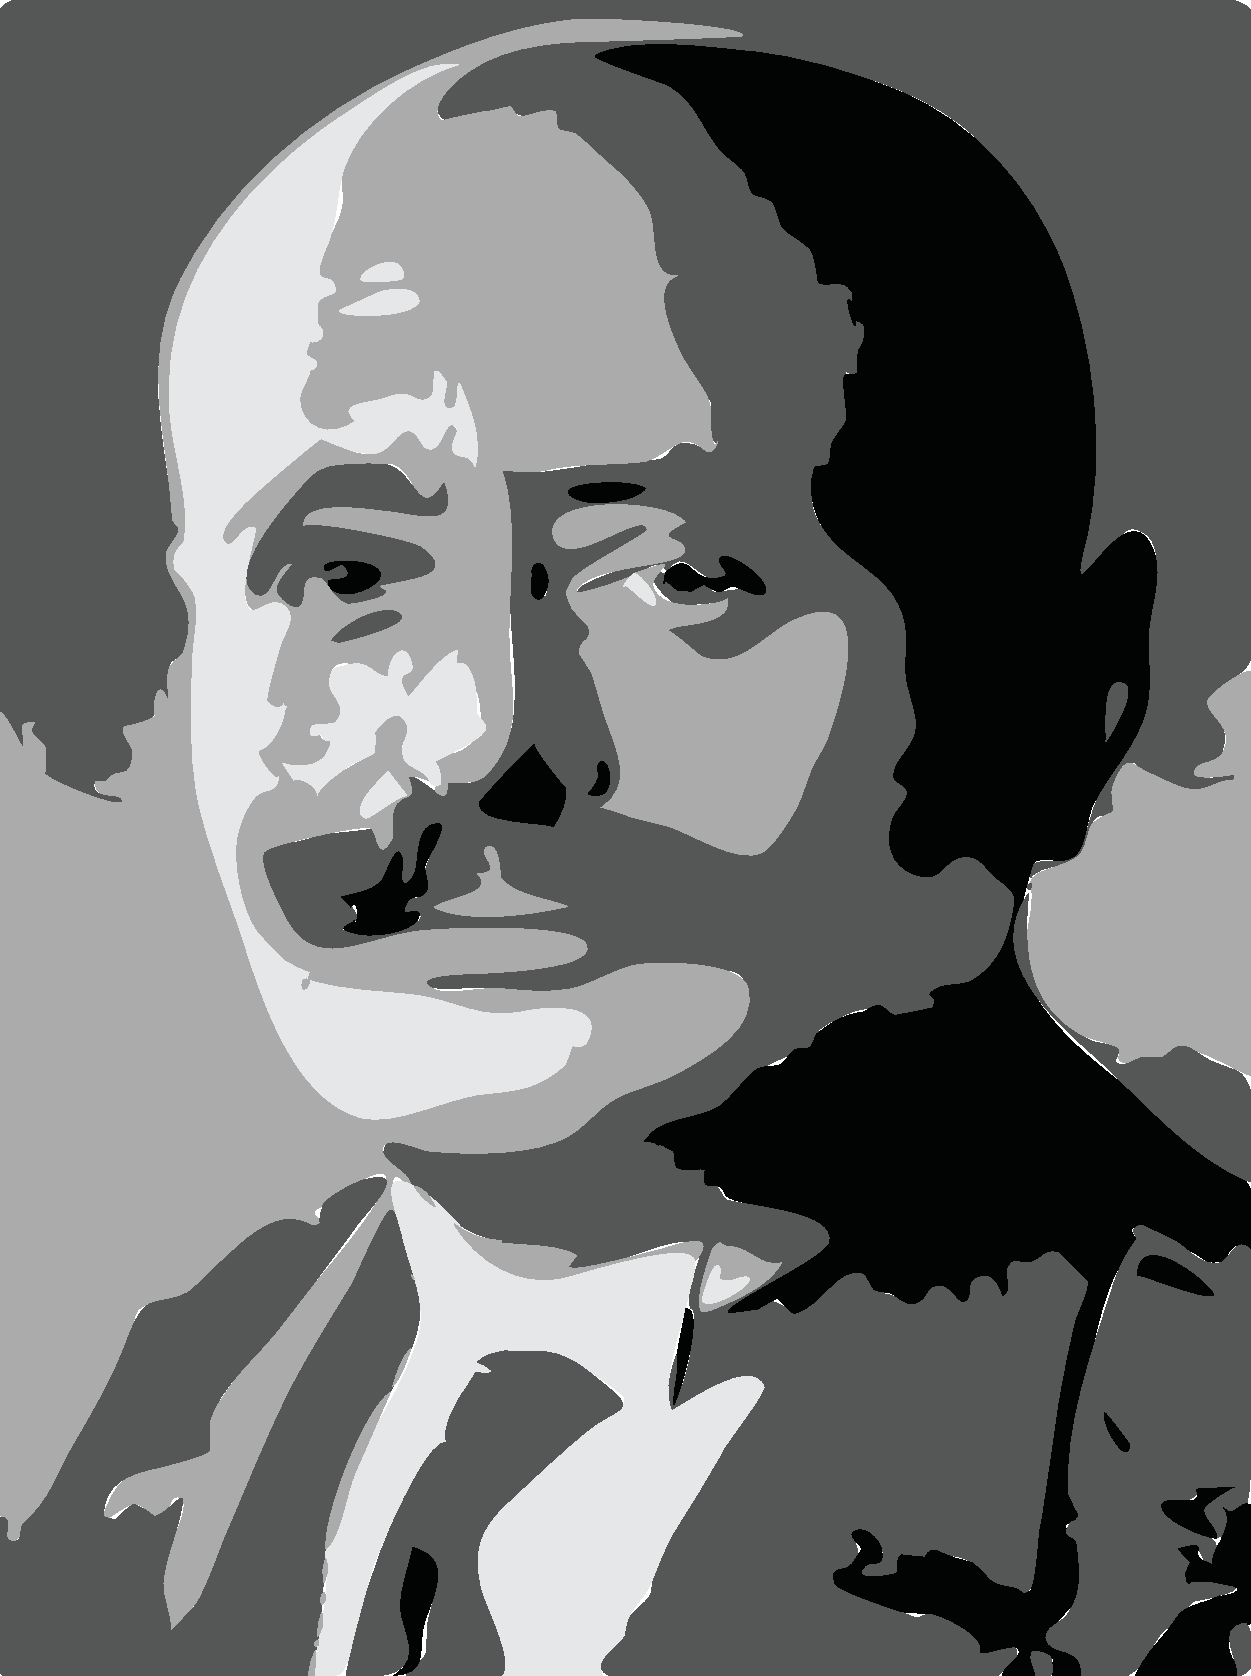
\includegraphics[width=.28\textwidth]{./fotos/calcasdos/Fubini.pdf}\\[5pt]
{\small \bfseries Guido Fubini}
\end{bio}

\begin{theorem}[Fubini]
  \label{teofub}\index{teorema!de Fubini}Sean
  $f\colon \mathbb{R}^{n}\rightarrow \mathbb{R}\cup \left\{\pm \infty \right\}$ una
  función integrable y $1\leq m<n$. Entonces existe un subconjunto
  nulo $Z$ de $\mathbb{R}^{n-m}$ tal que, para todo $y\in
  \mathbb{R}^{n-m}\smallsetminus Z$, la función
  $f^{y}\colon \mathbb{R}^{m}\rightarrow \mathbb{R}\cup \left\{\pm \infty \right\}$
  dada por
  \begin{equation*}
    f^{y}(x):=f(x,y)
  \end{equation*}
  es integrable. La función $F\colon \mathbb{R}^{n-m}\rightarrow
  \mathbb{R}$ dada por
  \begin{equation*}
    F(y):=
      \begin{cases}
        \int_{\mathbb{R}^{m}}f^{y} & 
        \text{si $y\in \mathbb{R}^{n-m}\smallsetminus Z$,} \\ 
        0 & \text{si $y\in Z$,}
      \end{cases}
  \end{equation*}
  también es integrable y
  \begin{equation}
    \int_{\mathbb{R}^{n-m}}F=\int_{\mathbb{R}^{n}}f.  \label{fub}
  \end{equation}
\end{theorem}

\begin{proof}
  Sean $h\in \mathcal{S}^{\ast }(\mathbb{R}^{n})$ y
  $g\in \mathcal{S}_{\ast }(\mathbb{R}^{n})$ tales que
  $h\leq f\leq g$. El teorema de Fubini para funciones semicontinuas
  (ver Proposición~\ref{propfub}) asegura que
  $h^{y}\in \mathcal{S}^{\ast }(\mathbb{R}^{m})$ y
  $g^{y}\in \mathcal{S}_{\ast }(\mathbb{R}^{m})$ para todo
  $y\in \mathbb{R}^{n-m}$ y que las funciones
  \begin{equation*}
    H(y):=\int_{\mathbb{R}^{m}}h^{y}\text{\qquad y\qquad }G(y):=\int_{\mathbb{R}^{m}}g^{y}
  \end{equation*}
  cumplen que $H\in \mathcal{S}^{\ast }(\mathbb{R}^{n-m})$, $G\in
  \mathcal{S}_{\ast }(\mathbb{R}^{n-m})$,
  \begin{equation*}
    \int_{\mathbb{R}^{n-m}}H=\int_{\mathbb{R}^{n}}h\text{\qquad y\qquad }\int_{\mathbb{R}^{n-m}}G=\int_{\mathbb{R}^{n}}g.
  \end{equation*}
  Para cada $y\in \mathbb{R}^{n-m}$ denotamos por
{\abovedisplayskip=7.5pt
\belowdisplayskip=7.5pt
  \begin{equation*}
    F_{1}(y):=\int_{\ast }f^{y}\text{\qquad y\qquad }F_{2}(y):=\int^{\ast }f^{y}.
  \end{equation*}
  Como $h^{y}\leq f^{y}\leq g^{y}$, se tiene que $H\leq F_{1}\leq
  F_{2}\leq G$ (ver Lema~\ref{intsupinf}). En consecuencia,
  \begin{equation*}
    \int_{\mathbb{R}^{n}}h=\int_{\mathbb{R}^{n-m}}H\leq \int_{\ast }F_{i}\leq
    \int^{\ast }F_{i}\leq \int_{\mathbb{R}^{n-m}}G=\int_{\mathbb{R}^{n}}g\text{,\qquad }i=1,2.
  \end{equation*}
  Dado que $f$ es integrable en $\mathbb{R}^{n}$, tomando el
  ínfimo sobre las funciones $g\in \mathcal{S}_{\ast
  }(\mathbb{R}^{n})$ tales que $g\geq f$ y el supremo sobre las
  funciones $h\in \mathcal{S}^{\ast }(\mathbb{R}^{n})$ tales que
  $h\leq f$, obtenemos
  \begin{equation*}
    \int_{\mathbb{R}^{n}}f\leq \int_{\ast }F_{i}\leq \int^{\ast }F_{i}\leq \int_{\mathbb{R}^{n}}f,\text{\qquad }i=1,2.
  \end{equation*}
  En consecuencia, $F_{1}$ y $F_{2}$ son integrables en
  $\mathbb{R}^{n-m}$ y
  \begin{equation*}
    \int_{\mathbb{R}^{n-m}}F_{1}=\int_{\mathbb{R}^{n-m}}F_{2}=\int_{\mathbb{R}^{n}}f.
  \end{equation*}
  Por el Corolario~\ref{corfuncfinita},
  $Z_i:=\left\{y\in\mathbb{R}^{n-m} : F_i(y)=\pm\infty\right\}$ es un
  subconjunto nulo de $\mathbb{R}^{n-m}$,
  la función 
  $\widetilde{F}_{i}\colon \mathbb{R}^{n-m}\rightarrow \mathbb{R}$ dada por
  \begin{equation*}
    \widetilde{F}_{i}(y):=
      \begin{cases}
        F_{i}(y) & \text{si
          $y\in\mathbb{R}^{n-m}\smallsetminus(Z_1\cup Z_2)$,} \\[3pt] 
        0 & \text{si $y\in Z_1\cup Z_2$,}
      \end{cases}
  \end{equation*}
  es integrable y
  \begin{equation*}
    \int_{\mathbb{R}^{n-m}}\widetilde{F}_{i}=\int_{\mathbb{R}^{n-m}}F_{i}=\int_{\mathbb{R}^{n}}f,\text{\qquad }i=1,2.
  \end{equation*}
  Como $\widetilde{F}_{i}$ toma valores en $\mathbb{R}$ tiene sentido
  considerar $\widetilde{F}_{2}-\widetilde{F}_{1}$ y, dado que
  $\widetilde{F}_{2}-\widetilde{F}_{1}\geq 0$ y
  $\int_{\mathbb{R}^{n-m}}(\widetilde{F}_{2}-\widetilde{F}_{1})=0$, el
  Corolario~\ref{corfunnula} asegura que 
  \begin{equation*}
    Z_{0}:=\left\{y\in
      \mathbb{R}^{n-m}:\widetilde{F}_{1}(y)\neq
      \widetilde{F}_{2}(y)\right\}
  \end{equation*}
  es nulo en $\mathbb{R}^{n-m}$.\ Entonces $Z:=Z_{0}\cup Z_{1}\cup Z_{2}$
  es nulo en $\mathbb{R}^{n-m}$ y, como
  \begin{equation*}
    \widetilde{F}_{i}(y)=F_{i}(y)\text{\qquad y\qquad }-\infty <\widetilde{F}_{1}(y)=\widetilde{F}_{2}(y)<\infty \text{\qquad }\forall y\in \mathbb{R}^{n-m}\smallsetminus Z,
  \end{equation*}
  de la definición de $F_{1}$ y $F_{2}$ se sigue que
  \begin{equation*}
    -\infty <\int_{\ast }f^{y}=\int^{\ast }f^{y}<\infty \text{\qquad }\forall
    y\in \mathbb{R}^{n-m}\smallsetminus Z.
  \end{equation*}}%
  Por tanto, $f^{y}$ es integrable y
  \begin{equation*}
    \int_{\mathbb{R}^{m}}f^{y}=F_{1}(y)=F_{2}(y)\text{\qquad }\forall y\in 
    \mathbb{R}^{n-m}\smallsetminus Z.
  \end{equation*}
  Finalmente, como $F_{1}=F$ c.d. en $\mathbb{R}^{n-m}$ y $F_{1}$ es
  integrable en $\mathbb{R}^{n-m}$, la Proposición~\ref{igualint}
  asegura que $F$ es integrable en $\mathbb{R}^{n-m}$ y
  \begin{equation*}
    \int_{\mathbb{R}^{n-m}}F=\int_{\mathbb{R}^{n-m}}F_{1}=\int_{\mathbb{R}^{n}}f.
  \end{equation*}
  Esto concluye la demostración.
\end{proof}

\begin{notation}
  La identidad \emph{(\ref{fub})} suele escribirse como
  \begin{equation*}
    \int_{\mathbb{R}^{n}}f(y,z)\,dy\,dz=\int_{\mathbb{R}^{n-m}}\biggl( \int_{\mathbb{R}^{m}}f(y,z)dy\biggr) dz.
  \end{equation*}
  Dado que el intercambio de variables $(y,z)\mapsto (z,y)$ es una
  transformación ortogonal, el \emph{Teorema~\ref{cvlinleb}}
  asegura que también
  \begin{equation*}
    \int_{\mathbb{R}^{n}}f(y,z)\,dy\,dz=\int_{\mathbb{R}^{m}}\biggl( \int_{\mathbb{R}^{n-m}}f(y,z)dz\biggr) dy.
  \end{equation*}
\end{notation}

\section{Teoremas de convergencia}

Daremos a continuación varios criterios importantes que garantizan
la integrabilidad del límite puntual de funciones integrables y
la posibilidad de expresar a la integral de dicho límite como el
límite de las correspondientes integrales.

El siguiente ejemplo muestra que no es cierto, en general, que el
supremo puntual de una sucesión no decreciente de funciones
integrables sea integrable.

\begin{example}
  \label{supnoint}Si $f_{k}:=1_{B^{n}(0,k)}$ es la función
  característica de la bola de radio $k$ con centro en el origen
  en $\mathbb{R}^{n}$, entonces $f_{k}$ es integrable y $f_{k}\leq
  f_{k+1}$ para todo $k\in \mathbb{N}$. Sin embargo,
  $1_{\mathbb{R}^{n}}=\sup_{k\in \mathbb{N}}f_{k}$ no es integrable.
\end{example}

Si el supremo puntual $f:=\sup_{k\in \mathbb{N}}f_{k}$ de una
sucesión no decreciente $(f_{k})$ de funciones integrables es
integrable, entonces
\begin{equation*}
  \lim_{k\rightarrow \infty }\int_{\mathbb{R}^{n}}f_{k}\leq \int_{\mathbb{R}^{n}}f<\infty .
\end{equation*}
El teorema que enunciaremos a continuación, afirma que basta con
que este límite sea finito para garantizar la integrabilidad de
$f$.

Nota que, si $(t_{k})$ es una sucesión no decreciente de
números reales entonces, para cualesquiera $k,i\in \mathbb{N}$, se
tiene que
\begin{equation*}
  t_{k+i}-t_{k}=\sum_{j=k+1}^{k+i}\left( t_{j}-t_{j-1}\right) .
\end{equation*}
Tomando el límite cuando $i\rightarrow \infty $ concluimos que
\begin{equation}
  \lim_{i\rightarrow \infty }t_{i}-t_{k}=\sum_{j=k+1}^{\infty }\left(
    t_{j}-t_{j-1}\right) .  \label{t-tk}
\end{equation}
Usaremos esta fórmula en la demostración del siguiente
resultado de Beppo Levi\footnote{Beppo Levi (1875-1961) nació en
  Turín, Italia y obtuvo el doctorado en la Universidad de
  Turín. En 1939 emigró a Argentina donde fue profesor de la
  Universidad Nacional del Litoral (hoy Universidad Nacional de
  Rosario).}.
\begin{bio}[H]
\centering
%
\includegraphics[width=.3\textwidth]{./fotos/calcasdos/Frechet.png}\\[5pt]

\includegraphics[width=.25\textwidth]{./fotos/calcasdos/Levi.pdf}\\[4pt]
{\small \bfseries Beppo Levi}
\vspace*{-4pt}
\end{bio}
{\abovedisplayskip=9pt
\belowdisplayskip=9pt%
\begin{theorem}[de convergencia monótona]
  \label{teocm}\index{teorema!de convergencia monótona}Si
  $f_{k}\colon \mathbb{R}^{n}\rightarrow \mathbb{R}\cup \left\{\pm \infty \right\}$ es
  integrable, $f_{k}\leq f_{k+1}$ para todo $k\in \mathbb{N}$ y
  \begin{equation*}
    \lim_{k\rightarrow \infty }\int_{\mathbb{R}^{n}}f_{k}<\infty ,
  \end{equation*}
  entonces $f:=\sup_{k\in \mathbb{N}}f_{k}$ es integrable y
  \begin{equation*}
    \int_{\mathbb{R}^{n}}f=\lim_{k\rightarrow \infty }\int_{\mathbb{R}^{n}}f_{k}.
  \end{equation*}
\end{theorem}}

\pagebreak

\begin{proof}
{\abovedisplayskip=7pt%
\belowdisplayskip=7pt%
  Como $f_{k}$ es integrable, la Proposición~\ref{funcfinita}
  asegura que el conjunto
  \begin{equation*}
    Z_{k}:=\left\{x\in \mathbb{R}^{n}:f_{k}(x)=\pm \infty \right\}
  \end{equation*}
  es nulo para todo $k\in \mathbb{N}$. Por tanto, $Z:=\cup
 _{k=1}^{\infty }Z_{k}$ es un subconjunto nulo de $\mathbb{R}^{n}$
  (ver Proposición~\ref{nulos}). Reemplazando los valores de
  $f_{k}$ en $Z$ por $0$ obtenemos funciones cuyo supremo puntual
  coincide con $f$ fuera de $Z$. Estas nuevas funciones también
  son integrables y la integral de cada una de ellas coincide con la
  de la función original (ver Proposición~\ref{igualint}). Por
  tanto, podemos suponer, sin perder generalidad, que $f_{k}$ toma
  valores en $\mathbb{R}$.

  De la fórmula (\ref{t-tk}) se sigue que
  \begin{equation*}
    f-f_{k}=\sum_{j=k+1}^{\infty }\left( f_{j}-f_{j-1}\right) .
  \end{equation*}
  Por tanto, usando el Lema~\ref{subadintsup} y la fórmula
  (\ref{t-tk}), obtenemos
  \begin{align*}
    \int^{\ast }\left( f-f_{k}\right) &\leq \sum_{j=k+1}^{\infty
    }\int^{\ast }(f_{j}-f_{j-1}) \\
    &=\sum_{j=k+1}^{\infty }\biggl( \int_{\mathbb{R}^{n}}f_{j}-\int_{\mathbb{R}^{n}}f_{j-1}\biggr) =\left( \lim_{i\rightarrow \infty }\int_{\mathbb{R}^{n}}f_{i}\right) -\int_{\mathbb{R}^{n}}f_{k}.
  \end{align*}
  Como $\lim_{i\rightarrow \infty }\int_{\mathbb{R}^{n}}f_{i}<\infty$,
  se tiene que
  $\lim_{k\rightarrow \infty }\left( \left( \lim_{i\rightarrow \infty
      }\int_{\mathbb{R}^{n}}f_{i}\right)
    -\int_{\mathbb{R}^{n}}f_{k}\right) =0$ y, en consecuencia,
  \begin{equation}
    \lim_{k\rightarrow \infty }\int^{\ast }\left( f-f_{k}\right) =0.  \label{eqcm1}
  \end{equation}
  Por otra parte, la Proposición~\ref{caractint} asegura que
  existe $\varphi_{k}\in \mathcal{C}_{c}^{0}(\mathbb{R}^{n})$ tal que
  \begin{equation*}
    \int^{\ast }\left\vert f_{k}-\varphi_{k}\right\vert <\frac{1}{k}.
  \end{equation*}
  Por tanto,
  \begin{equation*}
    \lim_{k\rightarrow \infty }\int^{\ast }\left\vert f-\varphi_{k}\right\vert
    \leq \lim_{k\rightarrow \infty }\int^{\ast }\left\vert f-f_{k}\right\vert
    +\lim_{k\rightarrow \infty }\int^{\ast }\left\vert f_{k}-\varphi
     _{k}\right\vert =0.
  \end{equation*}
  Esto prueba que $f$ es integrable y de la identidad~(\ref{eqcm1}) se obtiene que
  \begin{equation*}
    \int_{\mathbb{R}^{n}}f=\lim_{k\rightarrow \infty }\int_{\mathbb{R}^{n}}f_{k},
  \end{equation*}}%
  como afirma el enunciado.  
%   Esto prueba que $f$ es integrable y que
%   \begin{equation*}
%     \int_{\mathbb{R}^{n}}f=\lim_{k\rightarrow \infty }\int_{\mathbb{R}^{n}}\varphi_{k}.
%   \end{equation*}}%

% \noindent
%   De la desigualdad (\ref{eqcm1}) se sigue que
%   \begin{equation*}
%     \lim_{k\rightarrow \infty }\int_{\mathbb{R}^{n}}\left( f_{k}-\varphi
%      _{k}\right) =0,
%   \end{equation*}
%   lo que nos permite concluir que
%   \begin{equation*}
%     \lim_{k\rightarrow \infty }\int_{\mathbb{R}^{n}}f_{k}=\lim_{k\rightarrow
%       \infty }\left[ \int_{\mathbb{R}^{n}}\left( f_{k}-\varphi_{k}\right) +\int_{\mathbb{R}^{n}}\varphi_{k}\right] =\lim_{k\rightarrow \infty }\int_{\mathbb{R}^{n}}\varphi_{k}=\int_{\mathbb{R}^{n}}f,
%   \end{equation*}
%   como afirma el enunciado.
\end{proof}

El análogo para sucesiones decrecientes de funciones también
es válido.

\begin{corollary}
  \label{corcm}Si $f_{k}\colon \mathbb{R}^{n}\rightarrow \mathbb{R}\cup
  \left\{\pm \infty \right\}$ es integrable y $f_{k}\geq f_{k+1}$ para todo $k\in
  \mathbb{N}$, y
  \begin{equation*}
    \lim_{k\rightarrow \infty }\int_{\mathbb{R}^{n}}f_{k}>-\infty ,
  \end{equation*}
  entonces $f:=\inf_{k\in \mathbb{N}}f_{k}$ es integrable y
  \begin{equation*}
    \int_{\mathbb{R}^{n}}f=\lim_{k\rightarrow \infty }\int_{\mathbb{R}^{n}}f_{k}.
  \end{equation*}
\end{corollary}

\begin{proof}
  Este resultado se obtiene aplicando el Teorema~\ref{teocm} a la
  sucesión $(-f_{k})$.
\end{proof}

\begin{corollary}
  \label{cmunion}Sea $X_{1}\subset \cdots \subset X_{k}\subset \cdots
  $ una sucesión no decreciente de subconjuntos integrables de
  $\mathbb{R}^{n}$. Si la sucesión $(\left\vert X_{k}\right\vert
  )$ de sus medidas de Lebesgue en $\mathbb{R}^{n}$ está acotada,
  entonces $\cup_{k=1}^{\infty }X_{k}$ es integrable y
  \begin{equation*}
    \left\vert \bigcup_{k=1}^{\infty }X_{k}\right\vert
    =\lim_{k\rightarrow \infty }\left\vert X_{k}\right\vert .
  \end{equation*}
\end{corollary}

\begin{proof}
  Este resultado es consecuencia del Teorema~\ref{teocm} aplicado a la
  sucesión de funciones características $1_{X_{k}}$, ya que
  $\sup_{k\in \mathbb{N}}1_{X_{k}}=1_{\cup_{k=1}^{\infty }X_{k}}$.
\end{proof}

\begin{corollary}
  \label{cminterseccion}Sea $X_{1}\supset \cdots \supset X_{k}\supset
  \cdots $ una sucesión no creciente de subconjuntos integrables
  de $\mathbb{R}^{n}$. Entonces $\cap_{k=1}^{\infty }X_{k}$ es
  integrable y
  \begin{equation*}
    \left\vert \bigcap_{k=1}^{\infty }X_{k}\right\vert
    =\lim_{k\rightarrow \infty }\left\vert X_{k}\right\vert .
  \end{equation*}
\end{corollary}

\begin{proof}
  Este resultado es consecuencia del Corolario~\ref{corcm}\ aplicado a
  la sucesión de funciones características $1_{X_{k}}$, ya
  que $\inf_{k\in \mathbb{N}}1_{X_{k}}=1_{\cap_{k=1}^{\infty
    }X_{k}}$. Nota que $\int_{\mathbb{R}^{n}}1_{X_{k}}\geq 0$.
\end{proof}

Dadas funciones $f_{k}\colon \mathbb{R}^{n}\rightarrow \mathbb{R}\cup \left\{\pm
\infty \right\}$, denotamos por $\liminf_{k\rightarrow \infty
}f_{k}\colon \mathbb{R}^{n}\rightarrow \mathbb{R}\cup \left\{\pm \infty \right\}$\ y
por $\limsup_{k\rightarrow \infty }f_{k}\colon \mathbb{R}^{n}\rightarrow
\mathbb{R}\cup \left\{\pm \infty \right\}$ a las funciones
\begin{equation*}
  \Bigl( \liminf_{k\rightarrow \infty }f_{k}\Bigr) (x):=\liminf_{k\rightarrow
    \infty }f_{k}(x),\text{\qquad }\Bigl( \limsup_{k\rightarrow \infty
    }f_{k}\Bigr) (x):=\limsup_{k\rightarrow \infty }f_{k}(x)
\end{equation*}
(ver Definición~\ref{defliminfsup}).\ El siguiente resultado,
debido a Fatou\footnote{Pierre Joseph Louis Fatou (1878-1929)
  nació en Lorient, Francia. Estudió matemáticas en la
  École Normale Supérieure de Paris y trabajó como
  astrónomo en el observatorio de París.}, da condiciones para la
integrabilidad de $\liminf_{k\rightarrow \infty }f_{k}$.
\begin{bio}[H]
\centering
%\includegraphics[width=.3\textwidth]{./fotos/calcasdos/Frechet.png}\\[5pt]
\includegraphics[width=.25\textwidth]{./fotos/calcasdos/Fatou.pdf}\\[5pt]
{\small \bfseries Pierre Fatou}
\end{bio}

\begin{theorem}[Lema de Fatou]
  \label{fatou}\index{lema!de Fatou}Sea
  $f_{k}\colon \mathbb{R}^{n}\rightarrow \mathbb{R}\cup \left\{\pm \infty \right\}$ una
  sucesión de funciones integrables con las siguientes
  propiedades:

  \begin{enumerate}
  \item[(i)] existe una función integrable
    $g\colon \mathbb{R}^{n}\rightarrow \mathbb{R}\cup \left\{\pm \infty \right\}$ tal
    que $f_{k}\geq g$ para todo $k\in \mathbb{N}$,

  \item[(ii)] existe $M\in \mathbb{R}$ tal que
    \begin{equation*}
      \int_{\mathbb{R}^{n}}f_{k}\leq M\text{\qquad }\forall k\in \mathbb{N}.
    \end{equation*}
  \end{enumerate}

  Entonces $\liminf_{k\rightarrow \infty }f_{k}$ es integrable y
  \begin{equation*}
    \int_{\mathbb{R}^{n}}\liminf_{k\rightarrow \infty }f_{k}\leq
    \liminf_{k\rightarrow \infty }\int_{\mathbb{R}^{n}}f_{k}.
  \end{equation*}
\end{theorem}

\begin{proof}
  Fijemos $k\!\in\!\mathbb{N}$. Para cada $j\!\geq\! k$ definimos
  $f_{j,k}\!:=\!\min \left\{f_{i}:k\leq i\leq j\right\}$. Entonces, $f_{j,k}$ es
  integrable (ver Ejercicio~\ref{minmaxint}), $f_{j,k}\geq f_{j+1,k}$
  y $f_{j,k}\geq g$ para todo $j\in \mathbb{N}$. Por tanto,
  \begin{equation*}
    \lim_{j\rightarrow \infty }\int_{\mathbb{R}^{n}}f_{j,k}\geq \int_{\mathbb{R}^{n}}g>-\infty .
  \end{equation*}
  Por el Corolario~\ref{corcm}, se tiene que $g_{k}:=\inf_{j\geq
    k}f_{j,k}$ es integrable y
  \begin{equation}
    \int_{\mathbb{R}^{n}}g_{k}=\inf_{j\geq k}\int_{\mathbb{R}^{n}}f_{j,k}\leq
    \inf_{j\geq k}\int_{\mathbb{R}^{n}}f_{j}\leq M,  \label{fat}
  \end{equation}
  ya que $f_{j}\geq f_{j,k}$. Observa que $g_{k}=\inf_{j\geq
    k}f_{j}$. Como $g_{k}\leq g_{k+1}$ para todo $k\in \mathbb{N}$, el
  Teorema~\ref{teocm} asegura que $\sup_{k\in \mathbb{N}}g_{k}$ es
  integrable y, usando la desigualdad (\ref{fat}), obtenemos que
  \begin{equation*}
    \int_{\mathbb{R}^{n}}\sup_{k\in \mathbb{N}}\inf_{j\geq k}f_{j}=\int_{\mathbb{R}^{n}}\sup_{k\in \mathbb{N}}g_{k}=\sup_{k\in \mathbb{N}}\int_{\mathbb{R}^{n}}g_{k}\leq \sup_{k\in \mathbb{N}}\inf_{j\geq k}\int_{\mathbb{R}^{n}}f_{j},
  \end{equation*}
  como afirma el enunciado.
\end{proof}

El siguiente ejemplo muestra que, en general, no se cumple la igualdad
en el lema de Fatou, ni siquiera cuando la sucesión $(f_{k})$
converge puntualmente.

\begin{example}
  \label{ejemfat}Existen sucesiones $(f_{k})$ que satisfacen las
  hipótesis del lema de Fatou para las cuales se cumple la
  desigualdad estricta
  \begin{equation*}
    \int_{\mathbb{R}^{n}}\liminf_{k\rightarrow \infty
    }f_{k}<\liminf_{k\rightarrow \infty }\int_{\mathbb{R}^{n}}f_{k}.
  \end{equation*}
\end{example}

\begin{proof}
  Sea $f_{k}\colon \mathbb{R}\rightarrow \mathbb{R}$ la función
  $f_{k}(x):=\max \left\{k-k^{2}\left\vert x-\frac{1}{k}\right\vert ,0\right\}$.
  \begin{figure}[htb]
    \centering
    \begin{tikzpicture}[scale=1.55]
  \pgfmathsetmacro{\xO}{1}
  \draw[very thin] (-1,0)--(3,0);
  \draw[very thin] (0,0)--(0,2.1);
  \draw[dashed] (0.5,0)--(0.5,2);

  \draw[very thick] (-1,0)--(0,0)--(.5,2)--(1,0)--(3,0);
  \draw[very thin] (0,0.05)--(0,-0.05) node[below] {$0$};
  \draw[very thin] (1,0.05)--(1,-0.05) node[below] {$\frac{2}{k}$};
  \draw[very thin] (0.5,0.05)--(0.5,-0.05) node[below] {$\frac{1}{k}$};
%  \foreach \x in {0.5,1,1.5,2}
%  { \draw[very thin] (0.05,\x)--(-0.05,\x) node[left] {$\x$};
%  };
  \draw[very thin] (0.05,2)--(-0.05,2) node[left] {$k$};
  \draw (1,-0.6) node[below] {$y=f_k(x)$};
\end{tikzpicture}

  \end{figure}

  \noindent
  Entonces $f_{k}$ es integrable, $f_{k}\geq 0$ y
  \begin{equation*}
    \int_{\mathbb{R}}f_{k}=1\text{\qquad }\forall k\in \mathbb{N}\text{.}
  \end{equation*}
  Como $\lim_{k\rightarrow \infty }f_{k}(x)=0$ para todo $x\in
  \mathbb{R}$, se tiene que
  \begin{equation*}
    \int_{\mathbb{R}}\lim_{k\rightarrow \infty }f_{k}=0<1=\lim_{k\rightarrow
      \infty }\int_{\mathbb{R}}f_{k}.
  \end{equation*}
  Es decir, en este caso no se da la igualdad.
\end{proof}

Uno de los teoremas más importantes de la teoría de
integración es el teorema de convergencia dominada de
Lebesgue. Este teorema da una condición suficiente para la
integrabilidad del límite puntual de una sucesión de
funciones integrables: basta que la sucesión $(f_{k}) $ esté
dominada por una función integrable $g$, es decir, que $\left\vert
  f_{k}(x)\right\vert \leq g(x)$ p.c.t. $x\in \mathbb{R}^{n}$, para
que $\lim_{k\rightarrow \infty }f_{k}$ sea integrable. Dicha
condición asegura además que podemos intercambiar al
límite por la integral.

\begin{theorem}[de convergencia dominada]
  \label{teocd}\index{teorema!de convergencia dominada}Sean
  $f,f_{k}\colon \mathbb{R}^{n}\rightarrow \mathbb{R}\cup \left\{\pm \infty \right\}$
  funciones con las siguientes propiedades:

  \begin{enumerate}
  \item[(i)] $f_{k}$ es integrable,

  \item[(ii)] $f_{k}(x)\rightarrow f(x)$ p.c.t. $x\in \mathbb{R}^{n}$,

  \item[(iii)] existe una función integrable
    $g\colon \mathbb{R}^{n}\rightarrow \mathbb{R}\cup \left\{\pm \infty \right\}$ tal
    que, para cada $k\in \mathbb{N}$, se cumple que $\left\vert
      f_{k}(x)\right\vert \leq g(x)$ p.c.t. $x\in \mathbb{R}^{n}$.
  \end{enumerate}

  Entonces $f$ es integrable y
  \begin{equation*}
    \int_{\mathbb{R}^{n}}f=\lim_{k\rightarrow \infty }\int_{\mathbb{R}^{n}}f_{k}.
  \end{equation*}
\end{theorem}

\begin{proof}
  Los conjuntos
  \begin{align*}
    Z_{-1} &:=\left\{x\in \mathbb{R}^{n}:g(x)=\pm \infty \right\}, \\
    Z_{0} &:=\left\{x\in \mathbb{R}^{n}:\left( f_{k}(x)\right) 
    \text{ no converge a }f(x)\right\}, \\
    Z_{k} &:=\left\{x\in \mathbb{R}^{n}:\left\vert f_{k}(x)\right\vert >g(x)\right\},
  \end{align*}
  son nulos. Por tanto, $Z:=\cup_{k=-1}^{\infty }Z_{k}$ es nulo. Nota
  que $\left\vert f(x)\right\vert \leq g(x)<\infty $ para todo $x\in
  \mathbb{R}^{n}\smallsetminus Z$. Reemplazando $f_{k}(x)$, $f(x)$ y
  $g(x)$ por $0$ para todo $x\in Z$, podemos suponer sin perder
  generalidad que $f_{k}$, $f$ y $g$ toman valores en $\mathbb{R}$, y
  que
  \begin{equation}
    \lim_{k\rightarrow \infty }f_{k}(x)=f(x)\text{\qquad y\qquad }\left\vert
      f_{k}(x)\right\vert \leq g(x)\text{\qquad }\forall k\in \mathbb{N}\text{, \ }\forall x\in \mathbb{R}^{n}\text{.}  \label{fat2}
  \end{equation}
  Como $f_{k}\geq -g$ y
  \begin{equation*}
    \int_{\mathbb{R}^{n}}f_{k}\leq \int_{\mathbb{R}^{n}}g=:M\text{\qquad }\forall k\in \mathbb{N},
  \end{equation*}
  el lema de Fatou (ver Teorema~\ref{fatou}) asegura que $f$ es
  integrable y que
  \begin{equation}
    \int_{\mathbb{R}^{n}}f\leq \liminf_{k\rightarrow \infty }\int_{\mathbb{R}^{n}}f_{k}.  \label{cd2}
  \end{equation}
  Observa que las funciones $-f_{k}$ y $-f$ también satisfacen
  (\ref{fat2}). Por tanto,
  \begin{equation}
    -\int_{\mathbb{R}^{n}}f=\int_{\mathbb{R}^{n}}-f\leq \liminf_{k\rightarrow
      \infty }\int_{\mathbb{R}^{n}}-f_{k}=-\limsup_{k\rightarrow \infty
    }\int_{\mathbb{R}^{n}}f_{k}.  \label{cd3}
  \end{equation}
  De (\ref{cd2}) y (\ref{cd3}) se sigue que
  \begin{equation*}
    \int_{\mathbb{R}^{n}}f\leq \liminf_{k\rightarrow \infty }\int_{\mathbb{R}^{n}}f_{k}\leq \limsup_{k\rightarrow \infty }\int_{\mathbb{R}^{n}}f_{k}\leq \int_{\mathbb{R}^{n}}f.
  \end{equation*}
  En consecuencia,
  \begin{equation*}
    \int_{\mathbb{R}^{n}}f=\lim_{k\rightarrow \infty }\int_{\mathbb{R}^{n}}f_{k}
  \end{equation*}
  (ver Ejercicio~\ref{liminflim}). Esto concluye la demostración.
\end{proof}

Observa que las sucesiones de funciones de los Ejemplos
\ref{ejeminvtras},~\ref{ejemintnoconv},~\ref{supnoint} y~\ref{ejemfat}
no están dominadas por ninguna función integrable $g$
[Ejercicio~\ref{ejnodomi}].

La importancia del teorema de convergencia dominada quedará de
manifiesto en las múltiples aplicaciones que veremos en el resto
de este libro. Concluimos esta sección con dos corolarios
interesantes de los teoremas de convergencia monóntona y
convergencia dominada. En las secciones siguientes daremos algunas
aplicaciones de ellos.

{\abovedisplayskip=11.5pt
\belowdisplayskip=11.5pt
\begin{corollary}
  \label{intrest}Sean $X_{1}\subset \cdots \subset X_{k}\subset \cdots
  $ subconjuntos de $\mathbb{R}^{n}$, $X:=\bigcup_{k=1}^{\infty
  }X_{k}$ y $f\colon X\rightarrow \mathbb{R}$ una función tal que $f\mid
 _{X_{k}}\in \mathfrak{L}(X_{k})$ para todo $k\in \mathbb{N}$ y
  \begin{equation*}
    \lim_{k\rightarrow \infty }\int_{X_{k}}\left\vert f\right\vert <\infty .
  \end{equation*}
  Entonces $f\in \mathfrak{L}(X)$, $f\in \mathfrak{L}(X\smallsetminus
  X_{k})$ para todo $k\in \mathbb{N}$,
  \begin{equation*}
    \int_{X}f=\lim_{k\rightarrow \infty }\int_{X_{k}}f\text{\qquad y\qquad }\lim_{k\rightarrow \infty }\int_{X\smallsetminus X_{k}}\left\vert
      f\right\vert =0.
  \end{equation*}
\end{corollary}

\begin{proof}
  Como hemos convenido (ver Notación~\ref{notint}), identificamos
  a $f$ con su extensión trivial a $\mathbb{R}^{n}$. Denotamos por
  $f_{k}:=f1_{X_{k}}$. Por hipótesis $f_{k}\in
  \mathfrak{L}(\mathbb{R}^{n})$. En consecuencia, $\left\vert
    f_{k}\right\vert \in \mathfrak{L}(\mathbb{R}^{n})$ y, como
  $\left\vert f_{k}\right\vert \leq \left\vert f_{k+1}\right\vert $ y
  \begin{equation*}
    \lim_{k\rightarrow \infty }\int_{\mathbb{R}^{n}}\left\vert f_{k}\right\vert
    =\lim_{k\rightarrow \infty }\int_{X_{k}}\left\vert f\right\vert <\infty ,
  \end{equation*}
  el teorema de convergencia monótona (ver Teorema~\ref{teocm})
  asegura que $\vert f\vert\! =\!\sup_{k\in
    \mathbb{N}}\vert f_{k}\vert $ es integrable.

  Ahora, como $f_{k}(x)\rightarrow f(x)$ para todo
  $x\in \mathbb{R}^{n}$ y
  $\left\vert f_{k}(x)\right\vert \leq \left\vert f(x)\right\vert $
  para todo $x\in \mathbb{R}^{n}$ y $k\in \mathbb{N}$, el teorema de
  convergencia dominada (ver Teorema~\ref{teocd}) asegura que $f$ es
  integrable y que
  \begin{equation*}
    \int_{X}f=\lim_{k\rightarrow \infty }\int_{X_{k}}f
  \end{equation*}
  Entonces $f-f_{k}=f1_{X\smallsetminus X_{k}}$ es integrable y, en
  consecuencia, $\left\vert f-f_{k}\right\vert $ también lo
  es. Puesto que $\left\vert f(x)-f_{k}(x)\right\vert \rightarrow 0$
  para todo $x\in \mathbb{R}^{n}$ y $\left\vert
    f(x)-f_{k}(x)\right\vert \leq 2\left\vert f(x)\right\vert $ para
  todo $x\in \mathbb{R}^{n}$ y $k\in \mathbb{N}$, el teorema de
  convergencia dominada asegura que
  \begin{equation*}
    0=\lim_{k\rightarrow \infty }\int_{X}\left\vert f-f_{k}\right\vert
    =\lim_{k\rightarrow \infty }\int_{X\smallsetminus X_{k}}\left\vert
      f\right\vert ,
  \end{equation*}
  como afirma el enunciado.
\end{proof}

\begin{corollary}
  \label{convseriecd}Sea $f_{j}\colon \mathbb{R}^{n}\rightarrow \mathbb{R}$
  una sucesión de funciones integrables tales que
  \begin{equation*}
    \sum_{j=1}^{\infty }\int_{\mathbb{R}^{n}}\left\vert f_{j}\right\vert
    <\infty .
  \end{equation*}
  Entonces la serie $\sum_{j=1}^{\infty }f_{j}$ converge c.d. en
  $\mathbb{R}^{n}$ a una función integrable
  $f\colon \mathbb{R}^{n}\rightarrow \mathbb{R}$ y
  \begin{equation*}
    \lim_{k\rightarrow \infty }\int_{\mathbb{R}^{n}}\biggl\vert
      f-\sum_{j=1}^{k}f_{j}\biggr\vert =0.
  \end{equation*}
\end{corollary}}%

\begin{proof}
{\abovedisplayskip=7pt%
\belowdisplayskip=7pt%
  Denotemos por
  \begin{equation*}
    g_{k}:=\sum_{j=1}^{k}\left\vert f_{j}\right\vert \text{\qquad
      y\qquad }g:=\sum_{j=1}^{\infty }\left\vert f_{j}\right\vert
    =\sup_{k\in \mathbb{N}}g_{k}.
  \end{equation*}
  Como $g_{k}$ es integrable, $g_{k}\leq g_{k+1}$ y
  \begin{equation*}
    \lim_{k\rightarrow \infty }\int_{\mathbb{R}^{n}}g_{k}=\sum_{j=1}^{\infty }\int_{\mathbb{R}^{n}}\left\vert f_{j}\right\vert <\infty ,
  \end{equation*}
  el teorema de convergencia monótona asegura que $g$ es
  integrable. En consecuencia, por la Proposición~\ref{funcfinita},
  existe un subconjunto nulo $Z$ de $\mathbb{R}^{n}$ tal que
  \begin{equation*}
    g(x):=\sum_{j=1}^{\infty }\left\vert f_{j}(x)\right\vert <\infty 
    \text{\qquad }\forall x\in \mathbb{R}^{n}\smallsetminus Z.
  \end{equation*}
  \noindent
  Esto implica que la serie $\sum_{j=1}^{\infty }f_{j}(x)$ converge
  para todo $x\in \mathbb{R}^{n}\smallsetminus Z$.

  Definimos $f\colon \mathbb{R}^{n}\rightarrow \mathbb{R}$ como
  \begin{equation*}
    f(x):=
      \begin{cases}
        \sum_{j=1}^{\infty }f_{j}(x) & \text{si $x\in \mathbb{R}^{n}\smallsetminus Z$,} \\ 
        0 & \text{si $x\in Z$.}
      \end{cases}
  \end{equation*}
  Entonces $\sum_{j=1}^{k}f_{j}(x)\rightarrow f(x)$ p.c.t. $x\in
  \mathbb{R}^{n}$ y
  \begin{equation*}
    \biggl\vert \sum_{j=1}^{k}f_{j}(x)\biggr\vert \leq g(x)\text{\qquad }\forall x\in \mathbb{R}^{n},\text{ }\forall k\in \mathbb{N}\text{.}
  \end{equation*}
  El teorema de convergencia dominada asegura entonces que $f$ es
  integrable.  En consecuencia, $f-\sum_{j=1}^{k}f_{j}$ es integrable
  y, como
  \begin{equation*}
    f(x)-\sum_{j=1}^{k}f_{j}(x)\rightarrow 0\text{ \qquad }\forall x\in 
    \mathbb{R}^{n}\smallsetminus Z
  \end{equation*}
  y
  \begin{equation*}
    \biggl\vert f(x)-\sum_{j=1}^{k}f_{j}(x)\biggr\vert \leq \left\vert
      f(x)\right\vert +\biggl\vert \sum_{j=1}^{k}f_{j}(x)\biggr\vert \leq
    \left\vert f(x)\right\vert +g(x)\text{\qquad }\forall x\in \mathbb{R}^{n},\text{ }\forall k\in \mathbb{N}\text{,}
  \end{equation*}
  el teorema de convergencia dominada asegura que
  \begin{equation*}
    \lim_{k\rightarrow \infty }\int_{\mathbb{R}^{n}}\biggl\vert
      f-\sum_{j=1}^{k}f_{j}\biggr\vert =0,
  \end{equation*}
  como afirma el enunciado.}
\end{proof}

\vspace*{-15pt plus 5pt minus 5pt}

\section{La integral de funciones radiales}

Sean $0<a<b<\infty $. Considera el conjunto
\begin{equation*}
  A^{n}(a,b):=\left\{x\in \mathbb{R}^{n}:a\leq \left\Vert x\right\Vert \leq b\right\}.
\end{equation*}
Observa que $A^{n}(a,b)=\left[ \bar{B}^{n}(0,b)\smallsetminus
  \bar{B}^{n}(0,a)\right] \cup S^{n-1}(0,a)$. De la Proposición
\ref{vol}\ y los Ejemplos~\ref{volbola} y~\ref{volesfera} se sigue
entonces que
\begin{equation*}
  \vol_{n}(A^{n}(a,b))=(b^{n}-a^{n})\omega_{n},
\end{equation*}
donde $\omega_{n}$ es el volumen de la bola unitaria en
$\mathbb{R}^{n}$.
\pagebreak

Se dice que una función $g\colon A^{n}(a,b)\rightarrow \mathbb{R}$ es
\textbf{radial} \index{función!radial} si su valor depende
únicamente de $\left\Vert x\right\Vert $, es decir, si
$g(x)=f(\left\Vert x\right\Vert )$ donde $f\colon [a,b]\rightarrow
\mathbb{R}$. El siguiente resultado afirma que, si $f$ es continua, la
integral de $g$ se puede calcular en términos de la integral de
Riemann de $f$.

\begin{theorem}[Integral de una función radial]
  \index{integral!de una función radial}Si $f\colon [a,b]\rightarrow
  \mathbb{R}$ es una función continua, entonces
  \begin{equation*}
    \int_{A^{n}(a,b)}f(\left\Vert x\right\Vert )dx=n\omega
   _{n}\int_{a}^{b}f(t)t^{n-1}dt.
  \end{equation*}
\end{theorem}

\begin{proof}
  Para cada $k\in \mathbb{N}$ consideramos la partición
  $a=a_{0}<a_{1}<\cdots <a_{k}=b$ del intervalo $[a,b]$ tal que
  $a_{j}-a_{j-1}=\frac{1}{k}(b-a)$. Por simplicidad denotamos por
  $A:=A^{n}(a,b)$ y $A_{j}:=A^{n}(a_{j-1},a_{j})$. Entonces
  $A=A_{1}\cup \cdots \cup A_{k}$ y $A_{i}\cap A_{j}$ es nulo si
  $i\neq j$ (ver Ejemplo~\ref{volesfera}). Por tanto,
  \begin{equation*}
    \left\vert A\right\vert =\left\vert A_{1}\right\vert +\cdots +\left\vert
      A_{k}\right\vert .
  \end{equation*}
  El teorema del valor medio aplicado a la función $t\mapsto
  t^{n}$ asegura que existe $\xi_{j}\in (a_{j-1},a_{j})$ tal que
  \begin{equation*}
    a_{j}^{n}-a_{j-1}^{n}=n\xi_{j}^{n-1}(a_{j}-a_{j-1}).
  \end{equation*}
  Por tanto,
  \begin{equation*}
    \left\vert A_{j}\right\vert =(a_{j}^{n}-a_{j-1}^{n})\omega_{n}=n\xi
   _{j}^{n-1}(a_{j}-a_{j-1})\omega_{n}.
  \end{equation*}

  Considera la función
  \begin{equation*}
    g_{k}:=\sum_{j=1}^{k}f(\xi_{j})1_{A_{j}}.
  \end{equation*}
  Se tiene que
  \begin{equation*}
    \int_{A}g_{k}=\sum_{j=1}^{k}f(\xi_{j})\left\vert A_{j}\right\vert
    =n\omega_{n}\sum_{j=1}^{k}f(\xi_{j})\xi_{j}^{n-1}(a_{j}-a_{j-1}).
  \end{equation*}
  La suma que aparece en el término de la derecha es una suma de
  Riemann para la integral de la función $t\mapsto f(t)t^{n-1}$ en
  $[a,b]$. Por tanto, haciendo tender $k\rightarrow \infty $ obtenemos
  \begin{equation}
    \lim_{k\rightarrow \infty }\int_{A}g_{k}=n\omega
   _{n}\int_{a}^{b}f(t)t^{n-1}dt.  \label{rad2}
  \end{equation}
  Demostraremos a continuación que
  \begin{equation}
    \int_{A}f(\left\Vert x\right\Vert )dx=\lim_{k\rightarrow \infty
    }\int_{A}g_{k}(x)dx.  \label{rad3}
  \end{equation}

  Como $f$ es uniformemente continua en $[a,b]$, para cada
  $\varepsilon >0$ existe $k_{0}\in \mathbb{N}$ tal que
  \begin{equation*}
    \left\vert f(t)-f(s)\right\vert <\frac{\varepsilon }{\left\vert A\right\vert 
    }\text{\qquad si\enskip }\left\vert s-t\right\vert <\frac{b-a}{k}\text{\enskip con\enskip }k\geq
    k_{0}.
  \end{equation*}
  En consecuencia, dado que $\left\vert f(\left\Vert x\right\Vert
    )-g_{k}(x)\right\vert =\sum_{j=1}^{k}\left\vert f(\left\Vert
      x\right\Vert )-f(\xi_{j})\right\vert 1_{A_{j}}(x)$ p.c.t. $x\in
  A$, se tiene que
  \begin{align*}
    \int_{A}\left\vert f(\left\Vert x\right\Vert )-g_{k}(x)\right\vert dx
    &=\sum_{j=1}^{k}\int_{A_{j}}\left\vert f(\left\Vert x\right\Vert )-f(\xi
     _{j})\right\vert dx \\
    &\leq \sum_{j=1}^{k}\frac{\varepsilon }{\left\vert A\right\vert }\left\vert
      A_{j}\right\vert =\varepsilon \text{\qquad }\forall k\geq k_{0}.
  \end{align*}
  Esto demuestra (\ref{rad3}). Combinando las identidades (\ref{rad2})
  y (\ref{rad3}) se obtiene la identidad deseada.
\end{proof}

\begin{example}
  \label{anillo}Si $\gamma \in \mathbb{R}$ y $0<a<b<\infty $, entonces
  \begin{equation*}
    \int_{A^{n}(a,b)}\left\Vert x\right\Vert^{\gamma }dx=
      \begin{cases}
        \frac{n}{n+\gamma }\omega_{n}\left( b^{n+\gamma }-a^{n+\gamma }\right) & 
        \text{si $\gamma +n\neq 0$,} \\ 
        n\omega_{n}\left( \ln b-\ln a\right) & \text{si $\gamma +n=0$.}
      \end{cases}
  \end{equation*}
\end{example}

\begin{proof}
  Por el teorema anterior,
  \begin{equation*}
    \int_{A^{n}(a,b)}\left\Vert x\right\Vert^{\gamma }dx=n\omega
   _{n}\int_{a}^{b}t^{\gamma +n-1}dt.
  \end{equation*}
  Calculando la integral de la derecha se obtiene el resultado.
\end{proof}

Si $\gamma <0$ la función $x\mapsto \left\Vert x\right\Vert
^{\gamma }$ no está definida en $0$. Sin embargo, como $\left\{0\right\}$ es
un conjunto nulo, podemos extender esta función a una función
$\mathbb{R}^{n}\rightarrow \mathbb{R}$ dándole cualquier valor en
$0$, por ejemplo $0$.

\begin{proposition}
  \label{pot}\index{integral!de potencia@de $\left\Vert x\right\Vert
   ^{\gamma }$}Si $\gamma \in \mathbb{R}$ y $r>0$, entonces

  \begin{enumerate}
  \item[(a)] la función $x\mapsto \left\Vert x\right\Vert^{\gamma
    }$ es integrable en $\bar{B}^{n}(0,r)$ si y sólo si $\gamma
    +n>0$ y, en ese caso,
    \begin{equation*}
      \int_{\left\Vert x\right\Vert \leq r}\left\Vert x\right\Vert^{\gamma }dx=\frac{n\omega_{n}}{n+\gamma }r^{n+\gamma }\text{.}
    \end{equation*}

  \item[(b)] la función $x\mapsto \left\Vert x\right\Vert^{\gamma
    }$ es integrable en $\mathbb{R}^{n}\smallsetminus B^{n}(0,r)$ si y
    sólo si $\gamma +n<0$ y, en ese caso,
    \begin{equation*}
      \int_{\left\Vert x\right\Vert \geq r}\left\Vert x\right\Vert^{\gamma }dx=-\frac{n\omega_{n}}{n+\gamma }r^{n+\gamma }\text{.}
    \end{equation*}
  \end{enumerate}
\end{proposition}

\begin{proof}
  \emph{(a):} \ Sea $\varepsilon >0$. Del Ejemplo~\ref{anillo} se
  sigue que
  \begin{equation*}
    \lim_{\varepsilon \rightarrow 0}\int_{A^{n}(\varepsilon ,r)}\left\Vert
      x\right\Vert^{\gamma }dx=
      \begin{cases}
        \frac{n}{n+\gamma }\omega_{n}r^{n+\gamma } & \text{si $n+\gamma >0$,} \\ 
        \infty & \text{si $n+\gamma \leq 0$.}
      \end{cases}
  \end{equation*}
  Si $n+\gamma >0$,\ el Corolario~\ref{intrest} asegura que $x\mapsto
  \left\Vert x\right\Vert^{\gamma }$ es integrable en
  $\bar{B}^{n}(0,r)$ y que
  \begin{equation*}
    \int_{\left\Vert x\right\Vert \leq r}\left\Vert x\right\Vert^{\gamma
    }dx=\lim_{k\rightarrow \infty }\int_{A^{n}(\frac{1}{k},r)}\left\Vert
      x\right\Vert^{\gamma }dx=\frac{n}{n+\gamma }\omega_{n}r^{n+\gamma }\text{.}
  \end{equation*}
  Supongamos ahora que $\gamma +n\leq 0$. Si $x\mapsto \left\Vert
    x\right\Vert^{\gamma }$ fuera integrable en $\bar{B}^{n}(0,r)$,\
  se tendría que
  \begin{equation*}
    \int_{A^{n}(\varepsilon ,r)}\left\Vert x\right\Vert^{\gamma }dx\leq
    \int_{\left\Vert x\right\Vert \leq r}\left\Vert x\right\Vert^{\gamma
    }dx<\infty \text{\qquad }\forall \varepsilon \in (0,r).
  \end{equation*}
  Esto es una contradicción.

  La demostración de \emph{(b)} es análoga [Ejercicio~\ref{ejpot}].
\end{proof}

Anteriormente probamos que el producto de dos funciones integrables es
integrable si una de ellas es acotada (ver Lema~\ref{lemprod}). El
siguiente ejemplo muestra que esta última hipótesis es
importante.

\begin{example}
  \label{prodnoint}El producto de funciones integrables no es
  necesariamente integrable.
\end{example}

\begin{proof}
  La función $f(x):=\left\Vert x\right\Vert^{-n/2}$ es integrable
  en $\bar{B}^{n}(0,r)$, pero $f^{2}(x)=\left\Vert x\right\Vert^{-n}$
  no lo es.
\end{proof}

La Proposición~\ref{pot} nos permite dar un criterio muy útil
de integrabilidad para funciones $f\colon \mathbb{R}^{n}\rightarrow
\mathbb{R}$ en términos de su comportamiento al $\infty
$. Empezamos introduciendo el siguiente concepto.

\begin{definition}
  \label{deflocint}Sea $\Omega $ un subconjunto abierto de
  $\mathbb{R}^{n}$. Una función $f\colon \Omega \rightarrow \mathbb{R}$
  es \textbf{localmente integrable en }$\Omega $
  \index{función!localmente integrable}si, para todo subconjunto
  compacto $K$ de $\Omega $, la función $f\mid_{K}\colon K\rightarrow
  \mathbb{R}$ es integrable en $K$.
\end{definition}

Observa que cualquier función continua
$f\colon \mathbb{R}^{n}\rightarrow \mathbb{R}$ es localmente integrable (ver
Ejemplo~\ref{intsobrecomp}).  Denotamos por
\begin{equation}
  \mathfrak{L}_{\loc}(\Omega ):=\left\{f:\Omega \rightarrow \mathbb{R}:f\text{ es localmente integrable en }\Omega \right\}.  \label{Lloc}
\end{equation}
Una consecuencia del Corolario~\ref{intrest} es la siguiente.

\begin{proposition}
  \label{corlocint}Sea $\Omega $ un subconjunto abierto de
  $\mathbb{R}^{n}$. Entonces $f\in \mathfrak{L}(\Omega )$ si y
  sólo si $f\in \mathfrak{L}_{\loc}(\Omega )$ y $\int^{\ast
  }\left\vert f\right\vert <\infty $.
\end{proposition}

\begin{proof}
  $\Rightarrow )$: \ Claramente, si $f\in \mathfrak{L}(\Omega )$,
  entonces $f\in \mathfrak{L}_{\loc}(\Omega )$ y $\int^{\ast
  }\left\vert f\right\vert <\infty $.

  $\Leftarrow )$: \ Inversamente, supongamos que $f\in
  \mathfrak{L}_{\loc}(\Omega )$ y $\int^{\ast }\left\vert f\right\vert
  <\infty $. Para cada $k\in \mathbb{N}$ definimos
  \begin{equation*}
    \Omega_{k}:=\left\{x\in \Omega :\left\Vert x\right\Vert <k,\ \text{\ dist}(x,\partial \Omega )>\tfrac{1}{k}\right\}.
  \end{equation*}
  Entonces $\overline{\Omega }_{k}\subset \overline{\Omega }_{k+1}$ y
  $\Omega =\cup_{k=1}^{\infty }\overline{\Omega }_{k}$, donde
  $\overline{\Omega }_{k}$ es la cerradura de $\Omega_{k}$ en
  $\mathbb{R}^{n}$. Como $\overline{\Omega }_{k}$ es compacto, se
  tiene que $f\mid_{\overline{\Omega }_{k}}\in
  \mathfrak{L}(\overline{\Omega }_{k})$ y
  \begin{equation*}
    \int_{\overline{\Omega }_{k}}\left\vert f\right\vert \leq \int^{\ast
    }\left\vert f\right\vert <\infty \text{\qquad }\forall k\in \mathbb{N}.
  \end{equation*}
  Por el Corolario~\ref{intrest}, $f\in \mathfrak{L}(\Omega )$.
\end{proof}

\begin{corollary}[Criterio de integrabilidad]
  Si $f\in \mathfrak{L}_{\loc}(\mathbb{R}^{n})$ y existen $\varepsilon
  >0$, $M\geq 0$ y $r>0$ tales que
  \begin{equation*}
    \left\vert f(x)\right\vert \leq \frac{M}{\left\Vert x\right\Vert
     ^{n+\varepsilon }}\text{\qquad }\forall x\in \mathbb{R}^{n}\smallsetminus
    B^{n}(0,r),
  \end{equation*}
  entonces $f\in \mathfrak{L}(\mathbb{R}^{n})$.
\end{corollary}

\begin{proof}
  Como $\left\vert f\right\vert =\left\vert f\right\vert
  1_{\bar{B}^{n}(0,r)}+\left\vert f\right\vert
  1_{\mathbb{R}^{n}\smallsetminus \bar{B}^{n}(0,r)}$, se tiene que
  \begin{align*}
    \int^{\ast }\left\vert f\right\vert &\leq \int^{\ast }\left\vert
      f\right\vert 1_{\bar{B}^{n}(0,r)}+\int^{\ast }\left\vert f\right\vert 1_{\mathbb{R}^{n}\smallsetminus \bar{B}^{n}(0,r)} \\
    &\leq \int_{\left\Vert x\right\Vert \leq r}\left\vert f\right\vert
    +M\int_{\left\Vert x\right\Vert \geq r}\frac{1}{\left\Vert x\right\Vert
     ^{n+\varepsilon }}dx<\infty .
  \end{align*}
  La existencia de las dos últimas integrales se sigue de que
  $f\in \mathfrak{L}_{\loc}(\mathbb{R}^{n})$ y de la
  Proposición~\ref{pot}, respectivamente. La
  Proposición~\ref{corlocint}\ asegura que
  $f\in \mathfrak{L}(\mathbb{R}^{n})$.
\end{proof}

\section{El teorema de cambio de variable}

El teorema de cambio de variable para funciones continuas con soporte
compacto (ver Teorema~\ref{cv}) se generaliza a funciones integrables
como sigue.

\begin{theorem}[de cambio de variable]
  \label{teocv}\index{teorema!de cambio de variable}Sean $\Omega $ y
  $\Omega^{\prime }$ subconjuntos abiertos de $\mathbb{R}^{n}$ y
  $\varphi \colon \Omega \rightarrow \Omega^{\prime }$ un difeomorfismo de
  clase $\mathcal{C}^{1}$. Entonces, $f\in \mathfrak{L}(\Omega
 ^{\prime })$ si y sólo si $(f\circ \varphi )\left\vert \det
    \varphi^{\prime }\right\vert \in \mathfrak{L}(\Omega )$ y, en tal
  caso, se cumple que
  \begin{equation*}
    \int_{\Omega }f(\varphi (x))\left\vert \det \varphi^{\prime }(x)\right\vert
    dx=\int_{\Omega^{\prime }}f(y)dy.
  \end{equation*}
\end{theorem}

Reduciremos la demostración de este teorema al caso en el que
$f\in \mathcal{C}_{c}^{0}(\Omega^{\prime })$. Para ello requerimos el
siguiente resultado.

\begin{proposition}[Aproximación por funciones en
  $\mathcal{C}_{c}^{0}(\Omega )$]
  \label{aprox}Si $\Omega $ es abierto en $\mathbb{R}^{n}$ y $f\in
  \mathfrak{L}(\Omega )$ entonces existe una sucesión $f_{k}\in
  \mathcal{C}_{c}^{0}(\Omega )$ tal que
  \begin{equation*}
    \lim_{k\rightarrow \infty }\int_{\Omega }\left\vert f-f_{k}\right\vert =0.
  \end{equation*}
\end{proposition}

{\abovedisplayskip=8.5pt
\belowdisplayskip=8.5pt
\begin{proof}
  Sea $\varepsilon >0$. Basta probar que existe $f_{\varepsilon }\in
  \mathcal{C}_{c}^{0}(\Omega )$ tal que
  \begin{equation*}
    \int_{\Omega }\left\vert f-f_{\varepsilon }\right\vert <\varepsilon .
  \end{equation*}
  Como convenimos (ver Notación~\ref{notint}), identificamos a $f$
  con su extensión trivial a $\mathbb{R}^{n}$. Por la
  Proposición~\ref{caractint}\ existe $g\in
  \mathcal{C}_{c}^{0}(\mathbb{R}^{n})$ tal que
  \begin{equation}
    \int_{\mathbb{R}^{n}}\left\vert f-g\right\vert <\frac{\varepsilon }{3}.  \label{apro1}
  \end{equation}
  Considera la sucesión no decreciente de subconjuntos abiertos y
  acotados de $\Omega $,
  \begin{equation*}
    \Omega_{k}:=\left\{x\in \Omega :\left\Vert x\right\Vert <k,\ \text{\ dist}(x,\partial \Omega )>\tfrac{1}{k}\right\}.
  \end{equation*}
  Nota que $\ \Omega =\cup_{k=1}^{\infty }\Omega_{k}$. Como $\Omega
 _{k}$ es integrable se tiene que$\ g\mid_{\Omega_{k}}\in
  \mathfrak{L}(\Omega_{k})$ (ver Proposición~\ref{restrint}),\ y
  como además
  \begin{equation*}
    \lim_{k\rightarrow \infty }\int_{\Omega_{k}}\left\vert g\right\vert \leq
    \int_{\mathbb{R}^{n}}\left\vert g\right\vert <\infty ,
  \end{equation*}
  el Corolario~\ref{intrest} asegura que $g\in \mathfrak{L}(\Omega
  \smallsetminus \Omega_{k})$ y que
  \begin{equation*}
    \lim_{k\rightarrow \infty }\int_{\Omega \smallsetminus \Omega
     _{k}}\left\vert g\right\vert =0.
  \end{equation*}
  Escogemos $k_{0}\in \mathbb{N}$ tal que
  \begin{equation}
    \int_{\Omega \smallsetminus \Omega_{k_{0}}}\left\vert g\right\vert <\frac{\varepsilon }{3}.  \label{apro2}
  \end{equation}
  Por simplicidad escribimos $\Omega_{0}:=\Omega_{k_{0}}$. Sea
  $M:=\max_{x\in \overline{\Omega }_{0}}\left\vert g(x)\right\vert $.
  Como $1_{\Omega_{0}}\in S_{\ast }(\mathbb{R}^{n})$, existe $h\in
  \mathcal{C}_{c}^{0}(\mathbb{R}^{n})$ tal que $h\leq 1_{\Omega_{0}}$
  y
  \begin{equation*}
    \int_{\mathbb{R}^{n}}\left( 1_{\Omega_{0}}-h\right) <\frac{\varepsilon }{3M}.
  \end{equation*}
  Reemplazando $h$ por $\max \left\{0,h\right\}$, podemos suponer
  además que $h\geq 0$. Entonces $h(x)=0$ para todo
  $x\in \mathbb{R}^{n}\smallsetminus \Omega_{0}$ y, en consecuencia,
  $gh\in \mathcal{C}_{c}^{0}(\Omega )$. Más aún, usando el
  Ejercicio~\ref{adfinita} obtenemos
  \begin{align*}
    \int_{\Omega }\left\vert f-gh\right\vert &\leq \int_{\Omega }\left\vert
      f-g\right\vert +\int_{\Omega \smallsetminus \Omega_{0}}\left\vert
      g-gh\right\vert +\int_{\Omega_{0}}\left\vert g-gh\right\vert \\
    &\leq \int_{\mathbb{R}^{n}}\left\vert f-g\right\vert +\int_{\Omega
      \smallsetminus \Omega_{0}}\left\vert g\right\vert +M\int_{\mathbb{R}^{n}}\left( 1_{\Omega_{0}}-h\right) <\varepsilon .
  \end{align*}
  Esto concluye la demostración.
\end{proof}}%

Requerimos también información sobre la imagen de un conjunto
nulo bajo una función de clase $\mathcal{C}^{1}$. Se cumple lo
siguiente.

\begin{lemma}
  \label{imC1nulo}Si $\Omega $ es un subconjunto abierto de
  $\mathbb{R}^{n}$ y $\varphi \colon \Omega \rightarrow \mathbb{R}^{n}$ es
  de clase $\mathcal{C}^{1}$ entonces, para todo subconjunto nulo $Z$
  de $\Omega ,\ $el conjunto $\varphi (Z):=\left\{\varphi (z):z\in Z\right\}$ es
  nulo.
\end{lemma}

\begin{proof}
{\abovedisplayskip=8pt%
\belowdisplayskip=7pt%
  Sea $\Omega_{k}:=\left\{x\in \Omega :\left\Vert x\right\Vert <k,\:
    \dist(x,\partial \Omega )>\frac{1}{k}\right\}$. Dado que la unión
  numerable de conjuntos nulos es un conjunto nulo, basta probar que
  $\varphi (Z\cap \Omega_{k})$ es nulo para cada $k\in \mathbb{N}$.

  Fijemos $k\in \mathbb{N}$ y $\varepsilon >0$. Tomemos una familia
  numerable de cubos $Q_{j}$, $j\in \mathbb{N}$, tales que
  \begin{equation*}
    Z\cap \Omega_{k}\subset \bigcup_{j\in \mathbb{N}}Q_{j}\subset
    \Omega_{k}\qquad \text{y}\qquad \sum_{j=1}^{\infty }\left\vert
      Q_{j}\right\vert <\varepsilon .
  \end{equation*}
  Ésta se obtiene escogiendo un abierto $U$ tal que
  $Z\cap \Omega _{k}\subset U\subset \Omega_{k}$ y
  $\left\vert U\right\vert <\varepsilon $ (ver
  Proposición~\ref{aproxnulo}) y expresándolo como una unión de cubos,
  $U=\bigcup_{j\in \mathbb{N}}Q_{j}$, tales que
  int$\left( Q_{i}\right) \cap $ int$\left( Q_{j}\right) =\emptyset $
  si $i\neq j$ (ver Ejercicio~\ref{uninumrect}).

  Como $\overline{\Omega }_{k}$ es compacto y $\varphi^{\prime
  }\colon \Omega \rightarrow \mathcal{L}(\mathbb{R}^{n},\mathbb{R}^{n})$ es
  continua, se tiene que
  \begin{equation*}
    M_{k}:=\sup_{x\in \overline{\Omega }_{k}}\left\Vert \varphi^{\prime
      }(x)\right\Vert_{\mathcal{L}(\mathbb{R}^{n},\mathbb{R}^{n})}<\infty .
  \end{equation*}
  Del teorema del valor medio (ver Corolario~\ref{cortvm0}) y las
  desigualdades (\ref{compnormas}) se sigue entonces que, para
  cualesquiera $x,y\in Q_j$,
  \begin{equation*}
    \left\Vert \varphi (x)-\varphi (y)\right\Vert_{\infty }\leq \left\Vert
      \varphi (x)-\varphi (y)\right\Vert \leq M_{k}\left\Vert x-y\right\Vert \leq
    M_{k}\sqrt{n}\left\Vert x-y\right\Vert_{\infty }.
  \end{equation*}
  Esto implica que, si $Q_{j}$ es un cubo de semilado $\delta $,
  entonces $\varphi (Q_{j})$ está contenido en un cubo de semilado
  $M_{k}\sqrt{n}\delta $. Por tanto,
  \begin{equation*}
    \left\vert \varphi (Q_{j})\right\vert \leq M_{k}^{n}n^{n/2}\left\vert
      Q_{j}\right\vert \qquad \forall j\in \mathbb{N}.
  \end{equation*}
  Nota que $\varphi (Q_{j})$ es compacto y, por tanto, integrable. Se
  tiene entonces que
  \begin{equation*}
    \Biggl\vert \bigcup_{j=1}^{m}\varphi (Q_{j})\Biggr\vert \leq
    \sum_{j=1}^{m}\left\vert \varphi (Q_{j})\right\vert \leq
    M_{k}^{n}n^{n/2}\sum_{j=1}^{m}\left\vert Q_{j}\right\vert \leq
    M_{k}^{n}n^{n/2}\varepsilon \qquad \forall m\in \mathbb{N}.
  \end{equation*}
  El Corolario~\ref{cmunion}\ asegura que $\bigcup_{j=1}^{\infty
  }\varphi (Q_{j})$\ es integrable y que
  \begin{equation*}
    \Biggl\vert \bigcup_{j=1}^{\infty }\varphi (Q_{j})\Biggr\vert
    =\lim_{m\rightarrow \infty }\Biggl\vert \bigcup_{j=1}^{m}\varphi
      (Q_{j})\Biggr\vert \leq M_{k}^{n}n^{n/2}\varepsilon .
  \end{equation*}
  Como $\varphi (Z\cap \Omega_{k})\subset \bigcup_{j=1}^{\infty
  }\varphi (Q_{j})$, concluimos que
  \begin{equation*}
    \int^{\ast }1_{\varphi (Z\cap \Omega_{k})}\leq M_{k}^{n}n^{n/2}\varepsilon
    \qquad \forall \varepsilon >0.
  \end{equation*}
  Esto prueba que $\varphi (Z\cap \Omega_{k})$ es nulo.}
\end{proof}

Estamos listos para demostrar el teorema de cambio de variable.

{\abovedisplayskip=9pt
\belowdisplayskip=9pt
\begin{proof}[Demostración del Teorema~\ref{teocv}.] Sea $f\in
\mathfrak{L}(\Omega^{\prime })$. Por la Proposición~\ref{aprox}\
existe una sucesión $\left( f_{k}\right) $ en
$\mathcal{C}_{c}^{0}(\Omega^{\prime })$ tal que
\begin{equation}
  \lim_{k\rightarrow \infty }\int_{\Omega^{\prime }}\left\vert
    f-f_{k}\right\vert =0.  \label{tcv1}
\end{equation}
Reemplazando a $(f_{k})$ por una subsucesión, podemos suponer
además que existe un subconjunto nulo $Z$ de $\mathbb{R}^{n}$ tal
que
\begin{equation*}
  f_{k}(y)\rightarrow f(y)\qquad \forall y\in \Omega^{\prime }\smallsetminus Z
\end{equation*}
(ver Proposición~\ref{funnula}). Denotemos por
\begin{equation*}
  g_{k}:=(f_{k}\circ \varphi )\left\vert \det \varphi^{\prime }\right\vert
  \qquad \text{y}\qquad g:=(f\circ \varphi )\left\vert \det \varphi^{\prime
    }\right\vert .
\end{equation*}
Entonces, $g_{k}\in \mathcal{C}_{c}^{0}(\Omega )$,
\begin{equation*}
  g_{k}(x)\rightarrow g(x)\qquad \forall x\in \Omega \smallsetminus \varphi
 ^{-1}(Z)
\end{equation*}
y $\varphi^{-1}(Z)$ es nulo (ver Lema~\ref{imC1nulo}). El Teorema
\ref{cv}\ asegura que
\begin{equation}
  \int_{\Omega }g_{k}=\int_{\Omega }(f_{k}\circ \varphi )\left\vert \det
    \varphi^{\prime }\right\vert =\int_{\Omega^{\prime }}f_{k},  \label{tcv2}
\end{equation}
y que
\begin{align*}
  \int_{\Omega }\left\vert g_{k}-g_{j}\right\vert &=\int_{\Omega }\left(
    \left\vert f_{k}-f_{j}\right\vert \circ \varphi \right) \left\vert \det
    \varphi^{\prime }\right\vert =\int_{\Omega^{\prime }}\left\vert
    f_{k}-f_{j}\right\vert \\
  &\leq \int_{\Omega^{\prime }}\left\vert f_{k}-f\right\vert +\int_{\Omega
   ^{\prime }}\left\vert f-f_{j}\right\vert .
\end{align*}
De esta última desigualdad y la afirmación (\ref{tcv1}) se
sigue que existen $k_{1}<\cdots <k_{j}<k_{j+1}<\cdots $ tales que
\begin{equation*}
  \int_{\Omega }\left\vert g_{k_{j+1}}-g_{k_{j}}\right\vert <\frac{1}{2^{j}}.
\end{equation*}
En consecuencia, definiendo $g_{k_{0}}:=0$, concluimos que
\begin{equation*}
  \sum_{j=0}^{\infty }\int_{\Omega }\left\vert
    g_{k_{j+1}}-g_{k_{j}}\right\vert <\infty ,
\end{equation*}
Observa que
\begin{equation*}
  g_{k_{m}}=\sum_{j=0}^{m-1}(g_{k_{j+1}}-g_{k_{j}})
\end{equation*}
y que
\begin{equation*}
  g(x)=\sum_{j=0}^{\infty }(g_{k_{j+1}}(x)-g_{k_{j}}(x))\text{\qquad }\forall x\in \Omega \smallsetminus \varphi^{-1}(Z).
\end{equation*}
El Corolario~\ref{convseriecd} asegura entonces que $g$ es integrable
y que
\begin{equation*}
  \lim_{m\rightarrow \infty }\int_{\Omega }\left\vert g-g_{k_{m}}\right\vert
  =0.
\end{equation*}
Por tanto, usando las identidades (\ref{tcv1}) y (\ref{tcv2}),
concluimos que
\begin{equation*}
  \int_{\Omega }g=\lim_{m\rightarrow \infty }\int_{\Omega
  }g_{k_{m}}=\lim_{m\rightarrow \infty }\int_{\Omega^{\prime
    }}f_{k_{m}}=\int_{\Omega^{\prime }}f,
\end{equation*}
que es la identidad deseada.

Finalmente observa que, si $g:=(f\circ \varphi )\left\vert \det
  \varphi^{\prime }\right\vert $, entonces
\begin{equation*}
  f=(g\circ \varphi^{-1})\left\vert \det \left( \varphi^{-1}\right)^{\prime
    }\right\vert .
\end{equation*}
En consecuencia, $f\in \mathfrak{L}(\Omega^{\prime })$ si $g\in
\mathfrak{L}(\Omega )$. Esto concluye la demostración.
\end{proof}}

Veamos una aplicación del teorema anterior.

\begin{example}[Coordenadas polares]
  $f\in \mathfrak{L}(\mathbb{R}^{2})$ si y sólo si la función
  $(r,\theta )\mapsto rf(r\cos \theta ,r\sen \theta )$ es integrable
  en $[0,\infty )\times [0,2\pi ]$ y, en ese caso,
  \begin{equation*}
    \int_{\mathbb{R}^{2}}f=\int_{0}^{2\pi }\int_{0}^{\infty }rf(r\cos \theta
    ,r\sen \theta )\,dr\,d\theta .
  \end{equation*}
\end{example}

\begin{proof}
  Sean $\Omega :=(0,\infty )\times (0,2\pi )$ y $\Omega^{\prime
  }:=\mathbb{R}^{2}\smallsetminus \left\{(x,0):x\geq 0\right\}$. La función
  $\varphi \colon \Omega \rightarrow \Omega^{\prime }$ dada por $\varphi
  (r,\theta ):=(r\cos \theta ,r\sen \theta )$ es un difeomorfismo de
  clase $\mathcal{C}^{1}$ y $\left\vert \det \varphi^{\prime
    }(r,\theta )\right\vert =r$. Por el Teorema~\ref{teocv}, $f\in
  \mathfrak{L}(\Omega^{\prime })$ si y sólo si $(r,\theta
  )\mapsto rf(\varphi (r,\theta ))$ es integrable en $\Omega $, y
  \begin{equation*}
    \int_{\Omega^{\prime }}f=\int_{\Omega }rf(\varphi (r,\theta ))\,dr\,d\theta
    .
  \end{equation*}
  Como $\left( [0,\infty )\times [0,2\pi ]\right)
  \smallsetminus \Omega $ \ y $\ \mathbb{R}^{2}\smallsetminus \Omega
 ^{\prime }$ son subconjuntos nulos de $\mathbb{R}^{2}$, concluimos
  que $f\in \mathfrak{L}(\mathbb{R}^{2})$ si y sólo si $(r,\theta
  )\mapsto rf(r\cos \theta ,r\sen \theta )$ es integrable en
  $[0,\infty )\times [0,2\pi ]$ y
  \begin{equation*}
    \int_{\mathbb{R}^{2}}f=\int_{\Omega^{\prime }}f=\int_{\Omega }rf(\varphi
    (r,\theta ))\,dr\,d\theta =\int_{0}^{2\pi }\int_{0}^{\infty }rf(r\cos \theta
    ,r\sen \theta )\,dr\,d\theta ,
  \end{equation*}
  como afirma el enunciado.
\end{proof}

\pagebreak

\section{Ejercicios}

\begin{exercise}
  Prueba que $[0,1]\smallsetminus \mathbb{Q}$ es integrable y calcula
  su medida en $\mathbb{R}$.
\end{exercise}

\begin{exercise}
  El objetivo de este ejercicio es mostrar la existencia de
  subconjuntos nulos no numerables de $[0,1]$. El \textbf{conjunto de
    Cantor}\index{conjunto!de Cantor} $\mathfrak{C}$ se construye como
  sigue: Al intervalo $[0,1]$ le quitamos su \emph{tercio medio}
  $(\frac{1}{3},\frac{2}{3})$ y denotamos al conjunto restante por
  \begin{equation*}
    \mathfrak{C}_{1}:=[0,1]\smallsetminus \left( \tfrac{1}{3},\tfrac{2}{3}\right) .
  \end{equation*}
  A cada uno de los dos subintervalos cerrados de $\mathfrak{C}_{1}$
  le quitamos su tercio medio y denotamos al conjunto restante por
  \begin{equation*}
    \mathfrak{C}_{2}:=\mathfrak{C}_{1}\smallsetminus \left( \left( \tfrac{1}{9},\tfrac{2}{9}\right) \cup \left( \tfrac{7}{9},\tfrac{8}{9}\right) \right) .
  \end{equation*}
  Continuando de esta manera, a cada uno de los $2^{k}$ subintervalos
  cerrados de $\mathfrak{C}_{k}$ le quitamos su tercio medio y
  denotamos al conjunto restante por $\mathfrak{C}_{k+1}$. Definimos
  \begin{equation*}
    \mathfrak{C}:=\bigcap_{k=1}^{\infty }\mathfrak{C}_{k}.
  \end{equation*}
  Prueba que $\mathfrak{C}$ es nulo y no es numerable.
\end{exercise}

\begin{exercise}
  Para cada $\varepsilon >0$, define de manera explícita un
  subconjunto abierto integrable $\Omega $ de $\mathbb{R}^{n}$ tal que
  $\mathbb{Q}^{n}\subset \Omega $ y $\left\vert \Omega \right\vert
  <\varepsilon $.
\end{exercise}

\begin{exercise}

  \begin{enumerate}
  \item[(a)] Prueba que, si $Z$ es un subconjunto nulo de
    $\mathbb{R}^{n}$, entonces $\mathbb{R}^{n}\smallsetminus Z$ es
    denso en $\mathbb{R}^{n}$.

  \item[(b)] ¿Es cierto que, si un subconjunto
    integrable $X$ de $\mathbb{R}^{n}$\ tiene medida positiva entonces
    \emph{int}$(X)\neq \emptyset $?
  \end{enumerate}
\end{exercise}

\begin{exercise}
  Prueba que $Z$ es un subconjunto nulo de $\mathbb{R}^{n}$ si y
  sólo si $Z\cap Q$ es un subconjunto nulo de $\mathbb{R}^{n}$\
  para todo rectángulo $Q\subset \mathbb{R}^{n}$.
\end{exercise}

\begin{exercise}
  \label{uninumrect}Un \textbf{cubo} es un rectángulo
  $[a_{1},b_{1}]\times \cdots \times [a_{n},b_{n}]$ tal que
  $b_{i}-a_{i}=b_{1}-a_{1}\neq 0$ para todo $i=2,\dots,n$.

  \begin{enumerate}
  \item[(a)] Prueba que todo subconjunto abierto $\Omega $ de
    $\mathbb{R}^{n}$ es la unión de una familia numerable de cubos
    $Q_{k}$, $k\in \mathbb{N}$, tales que \emph{int}$\left(
      Q_{j}\right) \cap $ \emph{int}$\left( Q_{k}\right) =\emptyset $
    si $j\neq k$.

  \item[(b)] Sean $\Omega $ un subconjunto abierto de $\mathbb{R}^{n}$
    y $Z\subset \Omega $. Prueba que $Z$ es un subconjunto nulo de
    $\mathbb{R}^{n}$ si y sólo si para cada $\varepsilon >0$
    existe una familia numerable de cubos $Q_{k}$, $k\in \mathbb{N}$,
    tales que
    \begin{equation*}
      Z\subset \bigcup_{k\in \mathbb{N}}Q_{k}\subset \Omega \text{\qquad
        y\qquad }\sum_{k=1}^{\infty }\left\vert Q_{k}\right\vert
      <\varepsilon .
    \end{equation*}
    \emph{(Sugerencia: Usa la Proposición~\ref{aproxnulo} y el
      inciso }(a)\emph{.)}
  \end{enumerate}
\end{exercise}

\begin{exercise}
  \label{ejgrafnulo}

  \begin{enumerate}
  \item[(a)] Prueba que, si $1\leq m<n$, $\ X$ es una unión
    numerable de subconjuntos compactos de $\mathbb{R}^{m}$ y $\
    f\colon X\rightarrow \mathbb{R}^{n-m}$ es una función continua,
    entonces la gráfica de $f$,
    \begin{equation*}
      \emph{graf}(f):=\left\{(x,y)\in \mathbb{R}^{n}:x\in X\text{, }y=f(x)\right\},
    \end{equation*}
    es un subconjunto nulo de $\mathbb{R}^{n}$.

  \item[(b)] Prueba que, si $\Omega $ es abierto en $\mathbb{R}^{m}$ y
    $f\colon \Omega \rightarrow \mathbb{R}^{n-m}$ es continua, entonces la
    gráfica de $f$ es un subconjunto nulo de $\mathbb{R}^{n}$.

  \item[(c)] Prueba que todo subespacio vectorial propio de
    $\mathbb{R}^{n}$ es nulo.
  \end{enumerate}
\end{exercise}

\begin{exercise}
  \label{varnulo}Prueba que toda subvariedad $M$ de $\mathbb{R}^{n}$
  \emph{(ver Definición~\ref{defvar})} es un subconjunto nulo de
  $\mathbb{R}^{n}$. \emph{(Sugerencia: Usa el Teorema~\ref{teofi}.)}
\end{exercise}

\begin{exercise}
  Prueba que, si $\Omega $ es un subconjunto abierto de
  $\mathbb{R}^{n}$, $\varphi \colon \Omega \rightarrow \mathbb{R}^{m}$ es de
  clase $\mathcal{C}^{1}$ y $m>n$, entonces $\varphi (\Omega )$ es un
  subconjunto nulo de $\mathbb{R}^{m}$.
\end{exercise}

\begin{exercise}[Lema de Sard]
  \index{lema!de Sard}Sean $\Omega $ un subconjunto abierto de
  $\mathbb{R}^{n}$ y $\varphi \colon \Omega \rightarrow \mathbb{R}^{n}$ una
  función de clase $\mathcal{C}^{1}$. El conjunto
  \begin{equation*}
    K:=\left\{x\in \Omega :\det \varphi^{\prime }(x)=0\right\}
  \end{equation*}
  se llama el \textbf{conjunto de puntos críticos de} $\varphi $,
  su imagen $\varphi (K)$ se llama el \textbf{conjunto de valores
    críticos de} $\varphi $, y $\mathbb{R}^{n}\smallsetminus
  \varphi (K)$ se llama el \textbf{conjunto de valores regulares de
  }$\varphi $. Demuestra las siguientes afirmaciones:

  \begin{enumerate}
  \item[(a)] El conjunto de valores críticos de $\varphi $ es un
    subconjunto nulo de $\mathbb{R}^{n}$.

  \item[(b)] El conjunto de valores regulares de $\varphi $ es denso
    en $\mathbb{R}^{n}$.
  \end{enumerate}
\end{exercise}

\begin{exercise}
  \label{adfinita}Sean $X_{1},X_{2}$ subconjuntos integrables de
  $\mathbb{R}^{n}$ tales que $X_{1}\cap X_{2}$ es nulo. Denotamos por
  $X:=X_{1}\cup X_{2}$. Prueba que $f\colon X\rightarrow \mathbb{R}\cup
  \left\{\pm \infty \right\}$ es integrable en $X$ si y sólo si $f\mid
 _{X_{1}}$ es integrable en $X_{1}$ y $f\mid_{X_{2}}$ es integrable
  en $X_{2}$ y que, en ese caso,
  \begin{equation*}
    \int_{X}f=\int_{X_{1}}f+\int_{X_{2}}f.
  \end{equation*}
\end{exercise}

\begin{exercise}
  \label{noconvpunt}Considera la familia numerable de intervalos
  cerrados
  \begin{equation*}
    \left[ 0,\tfrac{1}{2}\right] ,\text{ }\left[ \tfrac{1}{2},1\right] ,\text{ }\left[ 0,\tfrac{1}{3}\right] ,\text{ }\left[ \tfrac{1}{3},\tfrac{2}{3}\right] ,\text{ }\left[ \tfrac{2}{3},1\right] ,\text{ }\left[ 0,\tfrac{1}{4}\right] ,\text{ }\left[ \tfrac{1}{4},\tfrac{1}{2}\right] ,\text{ }\left[ \tfrac{1}{2},\tfrac{3}{4}\right] ,\text{ }\left[ \tfrac{3}{4},1\right] ,\text{ }\ldots
  \end{equation*}
  Sea $f_{k}$ la función característica del $k$-ésimo
  intervalo de la lista.

  \begin{enumerate}
  \item[(a)] Prueba que
    \begin{equation*}
      \lim_{k\rightarrow \infty }\int_{\mathbb{R}}\left\vert f_{k}\right\vert =0.
    \end{equation*}

  \item[(b)] Prueba que $(f_{k}(x))$ no converge para ningún $x\in
    [0,1]$.

  \item[(c)] Exhibe una subsucesión $(f_{k_{j}})$ que converge a
    $0$ c.d.  en $\mathbb{R}$.
  \end{enumerate}
\end{exercise}

\begin{exercise}
  Prueba que si $Z$ es un subconjunto nulo de $\mathbb{R}^{m}$
  entonces, para cualquier subconjunto integrable $X$ de
  $\mathbb{R}^{n}$, el conjunto $Z\times X$ es un subconjunto nulo de
  $\mathbb{R}^{m}\times \mathbb{R}^{n}$.
\end{exercise}

\begin{exercise}
  Considera la función $f\colon \mathbb{R}^{2}\rightarrow \mathbb{R}$
  dada por
  \begin{equation*}
    f(x,y):=
      \begin{cases}
        \frac{x^{2}-y^{2}}{\left( x^{2}+y^{2}\right)^{2}} & \text{si $(x,y)\in
        (0,1)^{2}$,} \\ 
        0 & \text{si $(x,y)\in \mathbb{R}^{2}\smallsetminus (0,1)^{2}$.}
      \end{cases}
  \end{equation*}

  \begin{enumerate}
  \item[(a)] Prueba que la función $x\mapsto f(x,y)$ es integrable
    en $\mathbb{R}$ para todo $y\in \mathbb{R}$, la función
    $y\mapsto f(x,y)$ es integrable en $\mathbb{R}$ para todo $x\in
    \mathbb{R}$, y que las integrales
    \begin{equation*}
      \int_{\mathbb{R}}\biggl( \int_{\mathbb{R}}f(x,y)dx\biggr) dy,\text{\qquad }\int_{\mathbb{R}}\biggl( \int_{\mathbb{R}}f(x,y)dy\biggr) dx,
    \end{equation*}
    existen y son distintas.

  \item[(b)] ¿Es $f$ una función integrable en
    $\mathbb{R}^{2}$?
  \end{enumerate}
\end{exercise}

\begin{exercise}
  Considera la función $f\colon \mathbb{R}^{2}\rightarrow \mathbb{R}$
  dada por
  \begin{equation*}
    f(x,y):=
      \begin{cases}
        y^{-2} & \text{si $0<x<y<1$,} \\ 
        -x^{-2} & \text{si $0<y<x<1$,} \\ 
        0 & \text{en los otros casos},
      \end{cases}
  \end{equation*}
  y realiza un análisis análogo al del ejercicio anterior.
\end{exercise}

\begin{exercise}
  Usando el \emph{Ejercicio~\ref{riemannintervalo}} y el teorema de
  Fubini prueba que, si $Q$ es un rectángulo en $\mathbb{R}^{n}$ y
  $f\colon Q\rightarrow \mathbb{R}$ es continua, entonces la integral de
  Lebesgue de $f$ \emph{(Definición~\ref{intenX})} coincide con la
  integral dada por la \emph{Definición~\ref{defintrectangulo}}.
\end{exercise}

\begin{exercise}
  \label{ejmedext}Prueba que, si $X_{k}$ es un subconjunto integrable
  de $\mathbb{R}^{n}$ y
  \begin{equation*}
    \sum_{k=1}^{\infty }\left\vert X_{k}\right\vert <\infty ,
  \end{equation*}
  entonces $\bigcup_{k=1}^{\infty }X_{k}$ es un subconjunto integrable
  de $\mathbb{R}^{n}$ y
  \begin{equation*}
    \left\vert \bigcup_{k=1}^{\infty }X_{k}\right\vert \leq
    \sum_{k=1}^{\infty }\left\vert X_{k}\right\vert .
  \end{equation*}
\end{exercise}

\begin{exercise}
  Prueba que, si $f_{k}\colon \mathbb{R}^{n}\rightarrow \mathbb{R}\cup \left\{\pm
  \infty \right\}$ es integrable, $f_{k}\geq 0$ para todo $k\in \mathbb{N}$,
  y
  \begin{equation*}
    \sum_{k=1}^{\infty }\int_{\mathbb{R}^{n}}f_{k}<\infty ,
  \end{equation*}
  entonces $\sum_{k=1}^{\infty }f_{k}$ es integrable y
  \begin{equation*}
    \int_{\mathbb{R}^{n}}\sum_{k=1}^{\infty
    }f_{k}=\sum_{k=1}^{\infty }\int_{\mathbb{R}^{n}}f_{k}.
  \end{equation*}
\end{exercise}

\begin{exercise}
  \label{ejnodomi}Prueba, sin usar el teorema de convergencia
  dominada, que para las sucesiones de funciones $(f_{k})$ de los
  \emph{Ejemplos~\ref{ejeminvtras},~\ref{ejemintnoconv},~\ref{supnoint},y~\ref{ejemfat}}
  no existe ninguna función integrable
  $g\colon \mathbb{R}^{n}\rightarrow \mathbb{R}\cup \left\{\pm \infty
  \right\}$
  tal que $\left\vert f_{k}\right\vert \leq g$ c.d. en
  $\mathbb{R}^{n}$ para todo $k\in \mathbb{N}$.
\end{exercise}

\begin{exercise}
  Prueba que, si $f\colon \mathbb{R}^{n}\rightarrow \mathbb{R}$ es
  integrable, entonces
  \begin{equation*}
    \lim_{k\rightarrow \infty }\int_{\mathbb{R}^{n}\smallsetminus B^{n}(0,k)}f=0.
  \end{equation*}
\end{exercise}

\begin{exercise}[Dependencia continua de un parámetro]
  \label{dcp}Sean $Y\subset \mathbb{R}^{m}$, $y_{0}\in Y$ y
  $f\colon \mathbb{R}^{n}\times Y\rightarrow \mathbb{R}\cup \left\{\pm \infty \right\}$
  con las siguientes propiedades:

  \begin{enumerate}
  \item[(i)] Para cada $y\in Y$, la función $x\mapsto f(x,y)$ es
    integrable en $\mathbb{R}^{n}$.

  \item[(ii)] P.c.t. $x\in \mathbb{R}^{n}$, la función $y\mapsto
    f(x,y)$ es continua en $y_{0}$.

  \item[(iii)] Existe una función integrable
    $g\colon \mathbb{R}^{n}\rightarrow \mathbb{R}\cup \left\{\infty \right\}$ tal que,
    para todo $y\in Y$,
    \begin{equation*}
      \left\vert f(x,y)\right\vert \leq g(x)\text{\qquad c.d. en }\mathbb{R}^{n}.
    \end{equation*}
  \end{enumerate}

  Prueba que la función $F\colon Y\rightarrow \mathbb{R}$, dada por
  \begin{equation*}
    F(y):=\int_{\mathbb{R}^{n}}f(x,y)dx,
  \end{equation*}
  es continua en $y_{0}$.
\end{exercise}

\begin{exercise}[Derivación bajo el signo de integral]
  \label{dbi}Sea $f\colon \mathbb{R}^{n}\times (a,b)\rightarrow
  \mathbb{R}\cup \left\{\pm \infty \right\}$ una función con las siguientes
  propiedades:

  \begin{enumerate}
  \item[(i)] Para cada $t\in (a,b)$, la función $x\mapsto f(x,t)$
    es integrable en $\mathbb{R}^{n}$.

  \item[(ii)] P.c.t. $x\in \mathbb{R}^{n}$, la función $t\mapsto
    f(x,t)$ toma valores en $\mathbb{R}$\ y es diferenciable en
    $(a,b)$.

  \item[(iii)] Existe una función integrable
    $g\colon \mathbb{R}^{n}\rightarrow \mathbb{R}\cup \left\{\infty \right\}$ tal que,
    para todo $t\in (a,b)$,
    \begin{equation*}
      \left\vert \frac{\partial f}{\partial t}(x,t)\right\vert \leq g(x)\text{\qquad c.d. en }\mathbb{R}^{n}.
    \end{equation*}
  \end{enumerate}

  Prueba que la función $F\colon (a,b)\rightarrow \mathbb{R}$, dada por
  \begin{equation*}
    F(t):=\int_{\mathbb{R}^{n}}f(x,t)dx,
  \end{equation*}
  es diferenciable en $(a,b)$ y que
  \begin{equation*}
    F^{\prime }(t)=\int_{\mathbb{R}^{n}}\frac{\partial f}{\partial t}(x,t)dx.
  \end{equation*}
\end{exercise}

\begin{exercise}
  Sea $f\in
  \mathcal{C}_{c}^{1}(\mathbb{R}^{3}):=\mathcal{C}^{1}(\mathbb{R}^{3})\cap
  \mathcal{C}_{c}^{0}(\mathbb{R}^{3})$. Prueba que la función
  $F\colon \mathbb{R}^{3}\rightarrow \mathbb{R}$, dada por
  \begin{equation*}
    F(x):=\int_{\mathbb{R}^{3}}\frac{f(y)}{\left\Vert y-x\right\Vert }dy,
  \end{equation*}
  es de clase $\mathcal{C}^{1}$ y que sus derivadas parciales
  están dadas por
  \begin{equation*}
    \frac{\partial F}{\partial x_{i}}(x):=\int_{\mathbb{R}^{3}}\frac{1}{\left\Vert y-x\right\Vert }\frac{\partial f}{\partial y_{i}}(y)dy,\text{\qquad }i=1,2,3.
  \end{equation*}
\end{exercise}

\begin{exercise}
  Sea $\left\{X_{k}:k\in \mathbb{N}\right\}$ una familia de subconjuntos
  integrables de $\mathbb{R}^{n}$ tales que $X_{j}\cap X_{i}$ es nulo
  si $i\neq j$. Denotamos por $X:=\cup_{k=1}^{\infty }X_{k}$. Si
  $f\colon X\rightarrow \mathbb{R}$ es\ una función tal que $f\mid
 _{X_{k}}\in \mathfrak{L}(X_{k})$ para todo $k\in \mathbb{N}$ y
  existe $M\in \mathbb{R}$ tal que
  \begin{equation*}
    \sum_{j=1}^{k}\int_{X_{j}}\left\vert f\right\vert \leq M\text{\qquad 
    }\forall k\in \mathbb{N},
  \end{equation*}
  prueba que $f\in \mathfrak{L}(X)$ y
  \begin{equation*}
    \int_{X}f=\sum_{j=1}^{\infty }\int_{X_{j}}f.
  \end{equation*}
\end{exercise}

\begin{exercise}
  Prueba que, si $f\colon \mathbb{R}^n\to\mathbb{R}$ es integrable,
  $X_k$ es un subconjunto integrable de $\mathbb{R}^n$ y
  $\lim_{k\to\infty}\vert X_k\vert=0$, entonces
  \begin{equation*}
    \lim_{k\to\infty} \int_{X_k} f=0.
  \end{equation*}
\end{exercise}

\begin{exercise}
  Prueba que, para todo $r>0$, $1\leq i\leq n$,
  \begin{equation*}
    \int_{\bar{B}^{n}(0,r)}x_{i}^{2}\text{ }dx=\frac{\omega_{n}}{n+2}r^{n+2}.
  \end{equation*}
  \emph{(Sugerencia: Observa que, por la invariancia de la integral
    bajo transformaciones ortogonales,}
  \begin{equation*}
    \int_{\bar{B}^{n}(0,r)}x_{i}^{2}\text{ }dx=\int_{\bar{B}^{n}(0,r)}x_{j}^{2}\text{ }dx,
  \end{equation*}
  \emph{y calcula}
  \begin{equation*}
    \sum_{i=1}^{n}\int_{\bar{B}^{n}(0,r)}x_{i}^{2}\text{ }dx.\text{\emph{)}}
  \end{equation*}
\end{exercise}

\begin{exercise}
  Para $0\leq a<b<\infty $ y $n$ par, calcula la integral
  \begin{equation*}
    \int_{A^{n}(a,b)}\exp (-\left\Vert x\right\Vert^{2})dx.
  \end{equation*}
\end{exercise}

\begin{exercise}
  Para $0<a<b<\infty $, calcula la integral
  \begin{equation*}
    \int_{A^{n}(a,b)}\ln (\left\Vert x\right\Vert )dx.
  \end{equation*}
\end{exercise}

\begin{exercise}
  \label{ejpot}Sea $r>0$. Prueba que la función $x\mapsto
  \left\Vert x\right\Vert^{\gamma }$ es integrable en
  $\mathbb{R}^{n}\smallsetminus B^{n}(0,r)$ si y sólo si $\gamma
  +n<0$ y, en ese caso,
  \begin{equation*}
    \int_{\left\Vert x\right\Vert \geq r}\left\Vert x\right\Vert^{\gamma }dx=-\frac{n\omega_{n}}{n+\gamma }r^{n+\gamma }\text{.}
  \end{equation*}
\end{exercise}

\begin{exercise}
  Prueba que la función $f\colon \mathbb{R}^{n}\rightarrow \mathbb{R}$,
  $\ f(x):=\exp (-\left\Vert x\right\Vert^{2})$, es integrable en
  $\mathbb{R}^{n} $ y que
  \begin{equation*}
    \int_{\mathbb{R}^{n}}\exp (-\left\Vert x\right\Vert^{2})dx=\pi^{n/2}.
  \end{equation*}
\end{exercise}

\begin{exercise}
  ¿Para qué números $\gamma >0$ es $x\mapsto
  \left( \frac{1}{1-\left\Vert x\right\Vert^{2}}\right)^{\gamma }$
  integrable en $B^{n}(0,1)$? Calcula la integral
  \begin{equation*}
    \int_{\left\Vert x\right\Vert <1}\left( \frac{1}{1-\left\Vert x\right\Vert
       ^{2}}\right)^{\gamma }dx
  \end{equation*}
  para tales $\gamma $.
\end{exercise}

\begin{exercise}
  Sean $a_{1},\dots,a_{m}$ puntos distintos en $\mathbb{R}^{n}$,
  $m>n>1$, y sea $f\colon \mathbb{R}^{n}\rightarrow \mathbb{R}$, \
  \begin{equation*}
    f(x):=\prod_{i=1}^{m}\frac{1}{\left\Vert x-a_{i}\right\Vert }.
  \end{equation*}
  Prueba que $f$ es integrable en $\mathbb{R}^{n}$.
\end{exercise}

\begin{exercise}
  \label{prodloc}Prueba que, si $f\in
  \mathfrak{L}_{\loc}(\mathbb{R}^{m})$ y $g\in
  \mathfrak{L}_{\loc}(\mathbb{R}^{n-m})$ con $1\leq m<n$, entonces
  $f\odot g\in \mathfrak{L}_{\loc}(\mathbb{R}^{n})$, donde $(f\odot
  g)(x,y):=f(x)g(y)$ si $(x,y)\in \mathbb{R}^{m}\times
  \mathbb{R}^{n-m}\equiv \mathbb{R}^{n}$.
\end{exercise}

\begin{exercise}[Coordenadas esféricas]
  Sea $\varphi \colon [0,\infty )\times [0,\pi ]\times [0,2\pi
  ]\rightarrow \mathbb{R}^{3}$ la función $\varphi (r,\theta ,\phi
  ):=(r\sen \theta \cos \phi ,r\sen \theta \sen \phi ,r\cos \theta )$.
  Entonces $f\in \mathfrak{L}(\mathbb{R}^{3})$ si y sólo si la
  función $(r,\theta ,\phi )\mapsto f(\varphi (r,\theta ,\phi
  ))r^{2}\sen \theta $ es integrable en $[0,\infty )\times [0,\pi ]\times [0,2\pi ]$ y, en ese caso,
  \begin{equation*}
    \int_{\mathbb{R}^{3}}f=\int_{0}^{2\pi }\int_{0}^{\pi }\int_{0}^{\infty
    }f(r\sen \theta \cos \phi ,r\sen \theta \sen \phi ,r\cos \theta )r^{2}\sen
    \theta \,dr\,d\theta \,d\phi \text{.}
  \end{equation*}
\end{exercise}

\begin{exercise}[Coordenadas cilíndricas]
  Enuncia y demuestra el teorema de cambio de variable para el cambio
  de coordenadas $(r,\theta ,z)\mapsto (r\cos \theta ,r\sen \theta
  ,z)$.
\end{exercise}

\begin{exercise}
  Usando coordenadas esféricas calcula el volumen de la bola\break
  $\bar{B}_{3}(0,r):=\left\{x\in \mathbb{R}^{3}:\left\Vert x\right\Vert
  \leq r\right\}$.
\end{exercise}

\chapter{Los espacios de Lebesgue}

\label{capLp}En el espacio de funciones continuas con soporte compacto
$\mathcal{C}_{c}^{0}(\Omega )$ podemos considerar las normas
\begin{equation*}
  \left\Vert f\right\Vert_{p}:=\biggl( \int_{\Omega }\left\vert f\right\vert
   ^{p}\biggr)^{1/p},\qquad p\in [1,\infty ),
\end{equation*}
análogas a aquéllas en $\mathcal{C}^{0}[a,b]$ que consideramos
en el capítulo~\ref{capem}. Éstas aparecen en muchas
aplicaciones importantes, pero el espacio $\mathcal{C}_{c}^{0}(\Omega
)$ no resulta adecuado para tratar muchas de esas aplicaciones porque
no es completo.

Los espacios de Lebesgue $L^{p}(\Omega )$, que introduciremos en este
capítulo, son espacios de Banach y contienen a
$\mathcal{C}_{c}^{0}(\Omega )$ como subespacio denso. Sus elementos
son clases de equivalencia de funciones \textit{medibles} $f\colon \Omega
\rightarrow \mathbb{R}$ tales que $\left\vert f\right\vert^{p}$ es
integrable, y su norma es la que definimos arriba. Los espacios de
Lebesgue tienen una enorme relevancia en análisis y en diversas
áreas de las matemáticas, e importantes aplicaciones en la
física, la ingeniería, las finanzas y otras disciplinas.

Las funciones medibles son aquéllas que se obtienen como el
límite puntual de una sucesión de funciones integrables en
$\Omega $. A diferencia de las funciones integrables, las funciones
medibles tienen la ventaja de que el producto de funciones medibles y
la $p$-ésima potencia de una función medible resultan ser
funciones medibles. Se tiene además un criterio sencillo que
garantiza su integrabilidad: si $f$ es medible y está dominada por
una función integrable, entonces $f$ es integrable (ver Teorema
\ref{medint}). Para funciones medibles vale además el inverso del
teorema de Fubini (ver Teorema~\ref{teoton}).

Probaremos que el espacio $\mathcal{C}_{c}^{\infty }(\Omega )$ de
funciones de clase $\mathcal{C}^{\infty }$ con soporte compacto en
$\Omega $ es un subespacio denso de $L^{p}(\Omega )$. Para ello
introduciremos el \textit{producto de convolución}, que asocia a
un par de funciones $\rho \in \mathcal{C}_{c}^{\infty
}(\mathbb{R}^{n})$ y $f\in L^{p}(\mathbb{R}^{n})$ una función
$\rho \ast f\in \mathcal{C}^{\infty }(\mathbb{R}^{n})\cap
L^{p}(\mathbb{R}^{n})$. Escogiendo $\rho_{k}$ de manera adecuada, se
obtiene una sucesión $\rho_{k}\ast f$ de funciones con soporte
compacto que converge a $f$ en $L^{p}(\mathbb{R}^{n})$.

El producto de convolución tiene múltiples aplicaciones que
van desde la solución de problemas con condición de frontera
en ecuaciones diferenciales parciales, hasta el procesamiento de
señales digitales o de imágenes\footnote{Consulta,por ejemplo,
  el applet de M. Levoy, A. Adams, K. Dektar y N. Willett,
  \textit{Spacial Convolution}, applet para el curso Digital
  Photography (Spring 2011), Stanford University.\newline
  http://graphics.stanford.edu/courses/cs178/applets/convolution.html}.

Finalmente, estudiaremos la noción de compacidad en $L^{p}(\Omega
)$ y daremos condiciones que garantizan que un subconjunto
$\mathcal{K}$ de $L^{p}(\Omega )$ es compacto.

\section{Conjuntos y funciones medibles}

Denotemos por
\begin{equation*}
  \bar{B}^{n}(0,r):=\left\{x\in \mathbb{R}^{n}:\left\Vert x\right\Vert \leq r\right\}.
\end{equation*}

El volumen de un subconjunto abierto de $\mathbb{R}^{n}$ siempre
está definido (ver Definición~\ref{volabcom}), aun cuando
éste no sea integrable. Podemos extender la noción de volumen
como sigue.

\begin{definition}
  \label{defmedida}Un subconjunto $X$ de $\mathbb{R}^{n}$
  \index{conjunto!medible}es \textbf{(Lebesgue-) medible} si $X\cap
  \bar{B}^{n}(0,k)$ es integrable en $\mathbb{R}^{n}$ para todo $k\in
  \mathbb{N}$. Su\index{medida!de Lebesgue} \textbf{medida (de
    Lebesgue) }se define como
  \begin{equation*}
    \left\vert X\right\vert :=\lim_{k\rightarrow \infty }\left\vert X\cap 
      \bar{B}^{n}(0,k)\right\vert .
  \end{equation*}
\end{definition}

\begin{remark}
  (a) Observa que todo conjunto integrable es medible \emph{(ver
    Proposición~\ref{vol})}. El \emph{Corolario~\ref{cmunion}}\
  asegura que, en ese caso, la noción de medida dada por la
  \emph{Definición~\ref{defvolumen}}\ coincide con la dada
  aquí.

  (b) El recíproco no es cierto: claramente$,\ \mathbb{R}^{n}$ es
  medible pero no es integrable.

  (c) Nota también que si $X$ es medible y $\left\vert
    X\right\vert =0$ entonces $X$ es un conjunto nulo. Proponemos la
  demostración de esta afirmación como ejercicio
  \emph{[Ejercicio~\ref{med0nulo}]}.
\end{remark}

Los conjuntos medibles tienen las siguientes propiedades.

\begin{proposition}
  \label{conjmed}

  \begin{enumerate}
  \item[(a)] Si $X$ y $Y$ son subconjuntos medibles de
    $\mathbb{R}^{n}$, entonces $X\smallsetminus Y$ es medible.

  \item[(b)] Si $\left\{X_{j}:j\in \mathbb{N}\right\}$ es una familia numerable
    de subconjuntos medibles de $\mathbb{R}^{n}$, entonces
    \begin{equation*}
      \bigcup_{j=1}^{\infty }X_{j}\hspace{0.3in}\text{y}\hspace{0.3in}\bigcap_{j=1}^{\infty }X_{j}
    \end{equation*}
    son medibles.
  \end{enumerate}
\end{proposition}

\begin{proof}
  \emph{(a)} es consecuencia de la identidad
  \begin{equation*}
    \left( X\smallsetminus Y\right) \cap \bar{B}^{n}(0,k)=\left[ X\cap \bar{B}^{n}(0,k)\right] \smallsetminus \left[ Y\cap \bar{B}^{n}(0,k)\right]
  \end{equation*}
  y la Proposición~\ref{vol}.

  \emph{(b):} \ Sean $k\in \mathbb{N}$ y
  $Y_{m}:=\cup_{j=1}^{m}\left( X_{j}\cap \bar{B}^{n}(0,k)\right)
  $.
  Como $Y_{m}\subset \bar{B}^{n}(0,k)$, se tiene que la sucesión
  $\left( \left\vert Y_{m}\right\vert \right) $ es acotada. El
  Corolario~\ref{cmunion}\ asegura entonces que
  \begin{equation*}
    \bigcup_{m=1}^{\infty }Y_{m}=\bigcup_{j=1}^{\infty }\left(
      X_{j}\cap \bar{B}^{n}(0,k)\right) =\Biggl( \bigcup_{j=1}^{\infty
      }X_{j}\Biggr) \cap \bar{B}^{n}(0,k)
  \end{equation*}
  es integrable. En consecuencia, $\bigcup_{j=1}^{\infty }X_{j}$ es
  medible. De \emph{(a)} y la identidad
  \begin{equation*}
    \bigcap_{j=1}^{\infty }X_{j}=\mathbb{R}^{n}\smallsetminus
    \bigcup_{j=1}^{\infty }(\mathbb{R}^{n}\smallsetminus X_{j})
  \end{equation*}
  se sigue que $\bigcap_{j=1}^{\infty }X_{j}$ es medible.
\end{proof}

La proposición anterior proporciona muchos ejemplos de conjuntos
medibles, como los siguientes.

\begin{example}

  \begin{enumerate}
  \item[(a)] Todo subconjunto cerrado de $\mathbb{R}^{n}$ es medible.

  \item[(b)] Todo subconjunto abierto de $\mathbb{R}^{n}$ es medible.

  \item[(c)] Las uniones y las intersecciones numerables de
    subconjuntos abiertos o cerrados de $\mathbb{R}^{n}$ son medibles.
  \end{enumerate}
\end{example}

\begin{proof}
  \emph{(a):} \ Si $X$ es cerrado en $\mathbb{R}^{n}$, entonces $X\cap
  \bar{B}^{n}(0,k)$ es compacto y, en consecuencia, integrable en
  $\mathbb{R}^{n}$.

  \emph{(b)} y \emph{(c)} son consecuencia inmediata de \emph{(a)} y
  de la Proposición~\ref{conjmed}.
\end{proof}

No todos los subconjuntos de $\mathbb{R}^{n}$ son medibles. A
continuación daremos un ejemplo de un subconjunto de $\mathbb{R}$
que no lo es. Dicho ejemplo se debe a Vitali\footnote{Giuseppe Vitali
  (1875-1932) nació en Ravenna, Italia. Estudió en la Scuola
  Normale Superiore de Pisa, donde fue alumno de Luigi Bianchi y
  asistente de Ulisse Dini. Fue maestro de secundaria durante más
  de 20 años hasta que finalmente obtuvo una cátedra en la
  Universidad de Modena y Reggio Emilia.}.
\begin{bio}[H]
\centering
%\includegraphics[width=.3\textwidth]{./fotos/calcasdos/Frechet.png}\\[5pt]
\includegraphics[width=.25\textwidth]{./fotos/calcasdos/Vitali.pdf}\\[5pt]
{\small \bfseries Giuseppe Vitali}
\end{bio}
Requerimos el siguiente lema.

\begin{lemma}
  \label{lemnomed}Si $X$ es un subconjunto medible de $\mathbb{R}$ con
  $\left\vert X\right\vert >0$ entonces existe $\delta >0$ tal que
  $\left\{x-y:x,y\in X\right\}\supset (-\delta ,\delta )$.
\end{lemma}

\begin{proof}
  Reemplazando, de ser necesario, a $X$ por alguno de sus subconjuntos
  $X\cap \left[ -k,k\right] $ de medida positiva, podemos suponer sin
  perder generalidad que $X$ es integrable en $\mathbb{R}$. Escojamos
  un abierto $\Omega $ en $\mathbb{R}$ tal que $X\subset \Omega $ y
  $\left\vert \Omega \right\vert <\frac{4}{3}\left\vert X\right\vert $
  (ver Ejercicio~\ref{aproxabto}). $\Omega $ es la unión de una
  familia numerable de intervalos cerrados $I_{k}$, $k\in \mathbb{N}$,
  cuyos interiores son ajenos por pares (ver
  Ejercicio~\ref{uninumrect}). Usando el Corolario~\ref{cmunion}
  obtenemos
  \begin{equation*}
    \sum_{k=1}^{\infty }\left\vert I_{k}\right\vert =\left\vert \Omega
    \right\vert <\frac{4}{3}\left\vert X\right\vert =\frac{4}{3}\sum_{k=1}^{\infty }\left\vert X\cap I_{k}\right\vert .
  \end{equation*}
  Esta desigualdad implica que existe $k_{0}\in \mathbb{N}$ tal que
  $\left\vert I_{k_{0}}\right\vert <\frac{4}{3}\left\vert X\cap
    I_{k_{0}}\right\vert $. Sea $\delta :=\frac{1}{2}\left\vert
    I_{k_{0}}\right\vert $. Denotemos por$\ Y:=X\cap I_{k_{0}}$ y por
  \begin{equation*}
    Y+z:=\left\{y+z:y\in Y\right\}.
  \end{equation*}
  Probaremos a continuación que
  \begin{equation}
    (Y+z)\cap Y\neq \emptyset \text{\qquad }\forall z\in (-\delta ,\delta ).
    \label{intertras}
  \end{equation}
  Argumentando por contradicción, supongamos que $(Y+z)\cap
  Y=\emptyset $ para algún $z\in (-\delta ,\delta )$. Entonces
  \begin{align*}
    2\left\vert Y\right\vert &=\left\vert Y+z\right\vert +\left\vert
      Y\right\vert =\left\vert \left( Y+z\right) \cup Y\right\vert \\
    &\leq \left\vert \left( I_{k_{0}}+z\right) \cup I_{k_{0}}\right\vert \leq
    \left\vert I_{k_{0}}\right\vert +\left\vert z\right\vert \leq \frac{3}{2}\left\vert I_{k_{0}}\right\vert ,
  \end{align*}
  lo cual es imposible, ya que $\left\vert I_{k_{0}}\right\vert
  <\frac{4}{3}\left\vert Y\right\vert $.
  \begin{figure}[htb]
    \centering
    \begin{tikzpicture}[scale=1.4]
  \pgfmathsetmacro{\lI}{2}
  \pgfmathsetmacro{\lz}{3}

  \draw[very thick] (0,0.7)--({\lI},0.7);
  \draw[very thick] (\lz,0.7)--({\lI+\lz},0.7);
  \draw[very thin] (0,0.7)--({\lI+\lz},0.7);
  \draw[very thin,dashed] (0,0)--({\lI+\lz},0);

%  \draw[dashed] (0,-0.1)--(0,0.8);
%  \draw[dashed] (\lI,-0.1)--(\lI,0.8);
%  \draw[dashed] ({\lI+\lz},-0.1)--({\lI+\lz},0.8);

  \foreach \x in {0,\lI, \lz, {\lI+\lz}} do 
  {
    \draw[very thin] (\x,0.75)--(\x, 0.65);
  };

  \foreach \x in {0,\lI, {\lI+\lz}} do 
  {
    \draw[very thin] ({\x-0.05},-0.05)--({\x+0.05}, 0.05);
    \draw[very thin,dashed] (\x,0)--(\x,0.7);
  };

\draw ({0.5 * \lI}, 0.7) node[above] {$I_{k_0}$};
\draw ({\lz + (0.5 * \lI)}, 0.7) node[above] {$I_{k_0}+z$};

\draw ({0.5 * \lI}, 0) node[fill=white] {$|I_{k_0}|$};
\draw ({\lI + (0.5 * \lz)}, 0) node[fill=white] {$|z|$};

\end{tikzpicture}

    \end{figure}
  En consecuencia, se cumple (\ref{intertras}), es decir, para cada
  $z\in (-\delta ,\delta )$ existen $x,y\in Y$ tales que $x+z=y$. Esto
  concluye la demostración.
\end{proof}

\begin{theorem}[Vitali]
  \index{teorema!de Vitali}$\mathbb{R}$ contiene un subconjunto que no
  es medible.
\end{theorem}

\begin{proof}
  Considera la relación de equivalencia en $\mathbb{R}$\ dada por
  \begin{equation*}
    x\sim y\text{ \ si y sólo si \ }x-y\in \mathbb{Q}\text{,}
  \end{equation*}
  y escoge un elemento en cada clase de equivalencia. Sea $X$ el
  conjunto de dichos elementos. Entonces $\mathbb{R=\cup }_{q\in
    \mathbb{Q}}(X+q)$. Si $X$ fuera medible, necesariamente
  $\left\vert X\right\vert >0$\ pues, de lo contrario, $\mathbb{R}$
  sería nulo (ver Ejercicio~\ref{med0nulo}). De modo que, por el
  Lema~\ref{lemnomed}, existiría $\delta >0$ tal que $(-\delta
  ,\delta )\subset \left\{x-y:x,y\in X\right\}$, lo cual es imposible ya que
  \begin{equation*}
    \left\{x-y:x,y\in X\right\}\subset (\mathbb{R\smallsetminus Q)}\cup \left\{0\right\}.
  \end{equation*}
  Así concluimos que $X$ no es medible.
\end{proof}

De manera análoga se define el concepto de función medible:
una función es medible si cuando restringimos su dominio a
$\bar{B}^{n}(0,k)$ y proyectamos sus valores sobre el intervalo
$[-k,k]$ la función resulta integrable.

Más precisamente: dada $f\colon \mathbb{R}^{n}\rightarrow \mathbb{R}\cup
\left\{\pm \infty \right\}$ consideramos, para cada $k\in \mathbb{N}$, la
función $f_{[k]}\colon \mathbb{R}^{n}\rightarrow \mathbb{R}$ definida
como
\begin{equation}
  f_{[k]}:=\min \left\{\max \left\{f,-k\right\},k\right\}1_{\bar{B}^{n}(0,k)},  \label{fsubk}
\end{equation}
es decir,
\begin{equation*}
  f_{[k]}(x):=
  \begin{cases}
    k & \text{si }\left\Vert x\right\Vert \leq k\text{\quad y\quad }f(x)\in
    [k,\infty ), \\ 
    f(x) & \text{si }\left\Vert x\right\Vert \leq k\text{\quad y\quad }f(x)\in
    [-k,k], \\ 
    -k & \text{si }\left\Vert x\right\Vert \leq k\text{\quad y\quad }f(x)\in
    (-\infty ,-k], \\ 
    0 & \text{si }\left\Vert x\right\Vert >k.
  \end{cases}
\end{equation*}
\begin{figure}[htb]
  \centering
  \begin{tikzpicture}[scale=1.4]
  \pgfmathsetmacro{\escX}{2}
  \pgfmathsetmacro{\Xcub}{\escX*.8*.8*.8}
  \draw[very thin] (-2,0)--(2,0);
  \draw[very thin] (0,-2)--(0,2);

%  \draw[dashed] (0,-0.1)--(0,0.8);
%  \draw[dashed] (\lI,-0.1)--(\lI,0.8);
%  \draw[dashed] ({\lI+\lz},-0.1)--({\lI+\lz},0.8);

  \foreach \x in {-1,1} do 
  {
    \draw[very thin] (\x, 0.05)--(\x, -0.05);
  };
  \draw (0.1, -0.05) node[below] {$0$};
  \draw (-1,-0.05) node[below] {$-k$};
  \draw (1,-0.05) node[below] {$k$};

  \foreach \x in {-1, 1 } do 
  {
    \draw[very thin] (0.05,\x)--(-0.05, \x);
%    \draw[very thin,dashed] (\x,0)--(\x,0.7);
  };
  \draw (-0.05,-1) node[left] {$-k$};
  \draw (-0.05,1) node[left] {$k$};

\draw[very thick] (-2,0)--(-1,0);
\draw[very thick] (1,0)--(2,0);
\draw[domain=-1:1] plot ({\x},{\escX*\x*\x*\x});
\draw[domain=-.8:.8, very thick] plot ({\x},{\escX*\x*\x*\x});
\draw[very thick] (-1,-\Xcub)--(-.8,-\Xcub);
\draw[very thick] (1,\Xcub)--(.8,\Xcub);
\end{tikzpicture}

\end{figure}
\begin{definition}
  Una función $f\colon \mathbb{R}^{n}\rightarrow \mathbb{R}\cup \left\{\pm
  \infty \right\}$ es\index{función!medible} \textbf{(Lebesgue-) medible}
  si $f_{[k]}$ es integrable en $\mathbb{R}^{n}$ para todo $k\in
  \mathbb{N}$.
\end{definition}

Observa que, para cualquier subconjunto $X$ de $\mathbb{R}^{n}$ y
cualquier $k\in \mathbb{N}$,
\begin{equation}
  \left( 1_{X}\right)_{[k]}=1_{X\cap 
    \bar{B}^{n}(0,k)}.  \label{caracmed}
\end{equation}
En consecuencia, un subconjunto $X$ de $\mathbb{R}^{n}$\ es medible si
y sólo si $1_{X}$ es medible. El teorema de Vitali muestra pues
que no todas las funciones son medibles. Pero muchas funciones sí
lo son, por ejemplo las siguientes.

\begin{example}
  \label{L1locesmed}Toda función $f\in
  \mathfrak{L}_{\loc}(\mathbb{R}^{n})$ es medible. En particular, toda
  función continua $f\colon \mathbb{R}^{n}\rightarrow \mathbb{R}$ es
  medible.
\end{example}

\begin{proof}
  Si $f\in \mathfrak{L}_{\loc}(\mathbb{R}^{n})$ y $k\in \mathbb{N}$,
  entonces $f1_{\bar{B}^{n}(0,k)}$ es integrable en $\mathbb{R}^{n}$
  (ver Definición~\ref{deflocint}). En consecuencia, 
  \begin{equation*}
    f_{[k]}=\min
    \left\{\max
      \left\{f1_{\bar{B}^{n}(0,k)},-k1_{\bar{B}^{n}(0,k)}\right\},k1_{\bar{B}^{n}(0,k)}\right\}
  \end{equation*}
  es integrable en $\mathbb{R}^{n}$ (ver Ejercicio~\ref{minmaxint}).
\end{proof}

Probaremos ahora que las funciones medibles son precisamente
aquéllas que son límites puntuales de funciones integrables.

\begin{proposition}
  \label{medlimint}Sea $f\colon \mathbb{R}^{n}\rightarrow \mathbb{R}\cup
  \left\{\pm \infty \right\}$. Las siguientes afirmaciones son equivalentes:

  \begin{enumerate}
  \item[(a)] $f$\ es medible.

  \item[(b)] Existe una sucesión $f_{k}\colon \mathbb{R}^{n}\rightarrow
    \mathbb{R}$ de funciones integrables tales que
    $f_{k}(x)\rightarrow f(x)$ para todo $x\in \mathbb{R}^{n}$.

  \item[(c)] Existe una sucesión $f_{j}\colon \mathbb{R}^{n}\rightarrow
    \mathbb{R}\cup \left\{\pm \infty \right\}$ de funciones medibles tales que
    $f_{j}(x)\rightarrow f(x)$ para todo $x\in \mathbb{R}^{n}$.
  \end{enumerate}
\end{proposition}

\begin{proof}
  \emph{(a)}$\Rightarrow $\emph{(b):} \ Si $f$ es medible, entonces
  $f_{[k]}$ es integrable y $f_{[k]}(x)\rightarrow f(x)$ para todo
  $x\in \mathbb{R}^{n}$.

  \emph{(b)}$\Rightarrow $\emph{(c):} \ Esta implicación es obvia,
  ya que toda función integrable es medible.

  \emph{(c)}$\Rightarrow $\emph{(a):} \ Si $f_{j}\ $es medible y
  $f_{j}(x)\rightarrow f(x)$ entonces, para cada $k\in \mathbb{N}$, se
  tiene que $\left( f_{j}\right)_{[k]}$ es integrable y que
  $\lim_{j\rightarrow \infty }\left( f_{j}\right)
 _{[k]}(x)=f_{[k]}(x)$. Claramente, $|\left( f_{j}\right)_{[k]}|\leq
  k1_{\bar{B}^{n}(0,k)}$ para todo $j\in \mathbb{N}$. El teorema de
  convergencia dominada (Teorema~\ref{teocd}) asegura entonces que
  $f_{[k]}$ es integrable. Esto prueba que $f$ es medible.
\end{proof}

Concluimos lo siguiente.

\begin{example}
  \label{scmed}Si $f\in \mathcal{S}_{\ast }(\mathbb{R}^{n})\cup
  \mathcal{S}^{\ast }(\mathbb{R}^{n})$, entonces $f$ es medible.
\end{example}

\begin{proof}
  Toda función $f\in \mathcal{S}_{\ast }(\mathbb{R}^{n})\cup
  \mathcal{S}^{\ast }(\mathbb{R}^{n})$ es, por definición, el
  límite puntual de una sucesión de funciones en
  $\mathcal{C}_{c}^{0}(\mathbb{R}^{n})$. Así que, por la
  Proposición~\ref{medlimint}, $f$ es medible.
\end{proof}

\begin{proposition}
  \label{medlin}

  \begin{enumerate}
  \item[(a)] Si $f,g\colon \mathbb{R}^{n}\rightarrow \mathbb{R}$ son
    medibles y $\lambda ,\mu \in \mathbb{R}$, entonces $\lambda f+\mu
    g$ es medible.

  \item[(b)] Si $f,g\colon \mathbb{R}^{n}\rightarrow \mathbb{R}\cup \left\{\pm
    \infty \right\}$\ son medibles, entonces
    \begin{equation*}
      \left\vert f\right\vert ,\quad f^{+},\quad f^{-},\quad \max \left\{f,g\right\}\quad 
      \text{y}\quad \min \left\{f,g\right\}
    \end{equation*}
    son funciones medibles.
  \end{enumerate}
\end{proposition}

\begin{proof}
  \emph{(a):} \ Por la Proposición~\ref{medlimint} existen
  sucesiones de funciones integrables
  $f_{k},g_{k}\colon \mathbb{R}^{n}\rightarrow \mathbb{R}$ tales que
  $f_{k}(x)\rightarrow f(x)$ y $g_{k}(x)\rightarrow g(x)$ para todo
  $x\in \mathbb{R}^{n}$. Como $\lambda f_{k}+\mu g_{k}$ es integrable
  y $(\lambda f_{k}+\mu g_{k})(x)\rightarrow (\lambda f+\mu g)(x)$
  para todo $x\in \mathbb{R}^{n}$ la Proposición~\ref{medlimint}
  asegura que $\lambda f+\mu g$ es medible.

  \emph{(b)} se demuesta de manera análoga.
\end{proof}

El siguiente resultado caracteriza a las funciones medibles en
términos de conjuntos medibles.

\begin{proposition}
  \label{caractmed}$f\colon \mathbb{R}^{n}\rightarrow \mathbb{R}\cup \left\{\pm
  \infty \right\}$\ es medible si y sólo si 
\begin{equation*}
f^{\geq a}:=\left\{x\in\mathbb{R}^{n}:f(x)\geq a\right\}
\end{equation*}
es un subconjunto medible de
$\mathbb{R}^{n}$\ para todo $a\in \mathbb{R}$.
\end{proposition}

\begin{proof}
  $\Rightarrow )$: \ Si $f$ es medible, la Proposición~\ref{medlin}
  asegura que la función \
  $f_{k}:=\min \left\{ \max \left\{ k(f-a+\frac{1}{k}),0\right\}
    ,1\right\} $
  \ es medible para cualesquiera $k\in \mathbb{N}$, $a\in
  \mathbb{R}$.
  Nota que $f_{k}(x)=0$ si $f(x)\leq a-\frac{1}{k}$ y que $f_{k}(x)=1$
  si $f(x)\geq a$. En consecuencia,
  $f_{k}(x)\rightarrow 1_{f^{\geq a}}(x)$ para todo
  $x\in \mathbb{R}^{n}$. La Proposición~\ref{medlimint} asegura
  entonces que la función $1_{f^{\geq a}}$ es medible, y de
  (\ref{caracmed})\ se sigue que $f^{\geq a}$ es un conjunto medible.

  $\Leftarrow )$: \ Inversamente, supongamos que $f^{\geq a}$ es
  medible para cualquier $a\in \mathbb{R}$. Para cada $k\in
  \mathbb{N}$ subdividimos el intervalo $[-k,k]$ en intervalos de
  longitud $\frac{1}{2^{k}}$ y denotamos a los puntos de la
  partición por $a_{k,j}:=-k+\frac{j}{2^{k}}$, $\
  j=0,\dots,k2^{k+1}$. De la Proposición~\ref{conjmed} se sigue que
  los conjuntos
  \begin{align*}
        &X_{k,0}:=\left\{x\in \mathbb{R}^{n}:f(x)<a_{k,1}\right\}=\mathbb{R}^{n}\smallsetminus
        f^{\geq a_{k,1}}, \\ 
        &X_{k,j}:=\left\{x\in \mathbb{R}^{n}:a_{k,j}\leq f(x)<a_{k,j+1}\right\}=f^{\geq
          a_{k,j}}\smallsetminus f^{\geq a_{k,j+1}}, \\ 
        &X_{k,k2^{k+1}}:=\left\{x\in \mathbb{R}^{n}:a_{k,k2^{k+1}}\leq f(x)\right\}=f^{\geq k},
  \end{align*}
  son medibles, para todo $j=1,\ldots ,k2^{k+1}-1$. Por tanto, la función
  \begin{equation*}
    f_{k}:=\sum_{j=0}^{k2^{k+1}}a_{k,j}1_{X_{k,j}}
  \end{equation*}
  es medible.
\begin{figure}[H]
  \centering
  \begin{tikzpicture}[yscale=1.6, xscale=2]
  \draw[-latex',very thin] (-2,0)--(2,0);
  \draw[-latex',very thin] (0,-1.2)--(0,1.5);

  \foreach \x in {-1, 1 } do 
  {
    \draw[very thin] (0.05,\x)--(-0.05, \x);
  };

  \draw (0.01,-1.15) node[right] {$-k$};
  \draw (0.05,1) node[right] {$k$};
  \draw[very thin, densely dashed] (0,1)--(-0.740951,1);

\draw[domain=-1.8619:1.46209, samples=200] plot ({\x},{0.7*(-\x*\x*\x*\x -
  0.5*\x*\x*\x + 2*\x*\x) + 0.3});
\draw[densely dotted] (-1.8619,-1)--(1.46209,-1);
\draw[densely dotted] (-1.83384,-0.75)--(1.42399,-0.75);
\draw[densely dotted] (-1.80364,-0.5)--(1.38138,-0.5);
\draw[densely dotted] (-1.77087,-0.25)--(1.33269,-0.25);
\draw[densely dotted] (-1.59533,0.75)--(-0.572967,0.75);
\draw[densely dotted] (-1.64908,0.5)--(-0.373579,0.5);
\draw[densely dotted] (-1.69477,0.25)--(1.20322,0.25);

\draw[very thick] (-1.83384,-1)--(-2.5,-1);
\draw[very thick] (2.5,-1)--(1.42399,-1);
\draw[very thick] (-1.83384,-0.75)--(-1.80364,-0.75);
\draw[very thick] (1.38138,-0.75)--(1.42399,-0.75);
\draw[very thick] (-1.80364,-0.5)--(-1.77087,-0.5);
\draw[very thick] (1.33269,-0.5)--(1.38138,-0.5);
\draw[very thick] (-1.77087,-0.25)--(-1.73489,-0.25);
\draw[very thick] (1.27515,-0.25)--(1.33269,-0.25);
\draw[very thick] (-1.69477,0)--(-1.73489,0);
\draw[very thick] (1.27515,0)--(1.20322,0);
\draw[very thick] (-1.69477,0.25)--(-1.64908,0.25);
\draw[very thick] (1.1017,0.25)--(1.20322,0.25);
\draw[very thick] (-0.373579,0.25)--(.420961,0.25);
\draw[very thick] (-1.64908,0.5)--(-1.59533,0.5);
\draw[very thick] (-0.572967,0.5)--(-0.373579,0.5);
\draw[very thick] (0.420961,0.5)--(1.1017,0.5);
\draw[very thick] (-1.59533,0.75)--(-1.52846,0.75);
\draw[very thick] (-0.740951,0.75)--(-0.572967,0.75);
\draw[very thick] (-1.52846,1)--(-0.740951,1);

\draw[densely dotted] (-1.83384,-1)--(-1.83384,-.75);
\draw[densely dotted] (1.42399,-1)--(1.42399,-.75);
\draw[densely dotted] (-1.80364,-.75)--(-1.80364,-.5);
\draw[densely dotted] (1.38138,-.75)--(1.38138,-.5);
\draw[densely dotted] (-1.77087,-.5)--(-1.77087,-.25);
\draw[densely dotted] (1.33269,-.5)--(1.33269,-.25);
\draw[densely dotted] (-1.73489,-.25)--(-1.73489,0);
\draw[densely dotted] (1.27515,-.25)--(1.27515,0);
\draw[densely dotted] (-1.69477,0)--(-1.69477,0.25);
\draw[densely dotted] (1.20322,0)--(1.20322,0.25);
\draw[densely dotted] (-1.64908,0.25)--(-1.64908,0.5);
\draw[densely dotted] (-0.373579,0.25)--(-0.373579,0.5);
\draw[densely dotted] (0.420961,0.25)--(0.420961,0.5);
\draw[densely dotted] (1.1017,0.25)--(1.1017,0.5);
\draw[densely dotted] (-1.59533,0.5)--(-1.59533,0.75);
\draw[densely dotted] (-0.572967,0.5)--(-0.572967,0.75);
\draw[densely dotted] (-1.52846,0.75)--(-1.52846,1);
\draw[densely dotted] (-0.740951,0.75)--(-0.740951,1);

\end{tikzpicture}

\end{figure}

  Además, $f_{k}(x)\rightarrow f(x)$ para todo $x\in
  \mathbb{R}^{n}$. La Proposición~\ref{medlimint} asegura entonces
  que $f$ es medible.
\end{proof}

Recuerda que, en general, no es cierto que el producto de funciones
integrables es integrable (ver Ejemplo~\ref{prodnoint}). Pero sí
es una función medible, como veremos a continuación.

\begin{proposition}
  \label{prodmed}

  \begin{enumerate}
  \item[(a)] Si $f\colon \mathbb{R}^{n}\rightarrow \mathbb{R}$ es medible y
    $p\in (0,\infty )$, entonces $\left\vert f\right\vert^{p}$ es
    medible.

  \item[(b)] Si $f,g\colon \mathbb{R}^{n}\rightarrow \mathbb{R}$ son
    medibles, entonces $fg$ es medible.
  \end{enumerate}
\end{proposition}

\begin{proof}
  \emph{(a): } Por Proposición~\ref{medlin} sabemos que
  $\left\vert f\right\vert $ es medible. Entonces, la
  Proposición~\ref{caractmed} asegura que
  \begin{equation*}
    \left( \left\vert f\right\vert^{p}\right)^{\geq a}=
      \begin{cases}
        \left\vert f\right\vert^{\geq a^{1/p}} & \text{si $a\in (0,\infty )$,} \\ 
        \mathbb{R}^{n} & \text{si $a\in (-\infty ,0]$,}
      \end{cases}
  \end{equation*}
  es un conjunto medible para todo $a\in \mathbb{R}$ y, en
  consecuencia, $\left\vert f\right\vert^{p}$ es una función
  medible.

  \emph{(b):} \ Como
  \begin{equation*}
    fg=\frac{1}{2}\left[ (f+g)^{2}-f^{2}-g^{2}\right] ,
  \end{equation*}
  la afirmación \emph{(a)} con $p=2$ y la Proposición~\ref{medlin}
  implican que $fg$ es medible.
\end{proof}

Si modificamos los valores de una función medible sobre un
conjunto nulo, ésta continúa siendo medible.

\begin{proposition}
  \label{medcd}Sean $f,g\colon \mathbb{R}^{n}\rightarrow \mathbb{R}\cup
  \left\{\pm \infty \right\}$.\ Si $f$ es medible y $f(x)=g(x)$ p.c.t. $x\in
  \mathbb{R}^{n}$, entonces $g$ es medible.
\end{proposition}

\begin{proof}
  Si $f$ es medible y $f(x)=g(x)$ p.c.t. $x\in \mathbb{R}^{n}$,
  entonces $f_{[k]}$ es integrable y $f_{[k]}(x)=g_{[k]}(x)$
  p.c.t. $x\in \mathbb{R}^{n}$ para todo $k\in \mathbb{N}$. En
  consecuencia, $g_{[k]}$ es integrable (ver
  Proposición~\ref{igualint}). Esto prueba que $g$ es medible.
\end{proof}

El siguiente criterio de integrabilidad jugará un papel muy
importante en la siguiente sección.

\begin{theorem}
  \label{medint}Si $f\colon \mathbb{R}^{n}\rightarrow \mathbb{R}\cup \left\{\pm
  \infty \right\}$ es medible y existe una función integrable
  $g\colon \mathbb{R}^{n}\rightarrow \mathbb{R}\cup \left\{\infty \right\}$ tal que
  $\left\vert f(x)\right\vert \leq g(x)$ p.c.t. $x\in \mathbb{R}^{n}$,
  entonces $f$ es integrable.
\end{theorem}

\begin{proof}
  Si $f$ es medible, entonces $f_{[k]}$ es integrable para todo
  $k\in \mathbb{N}$. Como $f_{[k]}(x)\rightarrow f(x)$ para todo
  $x\in \mathbb{R}^{n}$ y
  $\left\vert f_{[k]}(x)\right\vert \leq \left\vert f(x)\right\vert
  \leq g(x)$
  p.c.t. $x\in \mathbb{R}^{n}$ y todo $k\in \mathbb{N}$, el teorema de
  convergencia dominada (Teorema~\ref{teocd}) asegura que $f$ es
  integrable.
\end{proof}

Recuerda que, si $f$ es integrable, entonces $\left\vert f\right\vert
$ lo es (ver Proposición~\ref{valabsint}). Del teorema anterior se
obtiene inmediatamente el recíproco para funciones medibles.

\begin{corollary}
  \label{valabsinteq}Si $f\colon \mathbb{R}^{n}\rightarrow \mathbb{R}\cup
  \left\{\pm \infty \right\}$\ es medible y $\left\vert f\right\vert $ es
  integrable, entonces $f$ es integrable.
\end{corollary}

Tonelli\footnote{Leonida Tonelli (1885-1946) nació en Gallipoli,
  Puglia, Italia. Estudió en la Universidad de Bologna donde fue
  alumno de Cesare Arzelà.  Fue profesor en las universidades de
  Parma, Bologna y Pisa.} demostró que para funciones medibles
vale el recíproco del teorema de Fubini.
\begin{bio}[H]
\centering
%\includegraphics[width=.3\textwidth]{./fotos/calcasdos/Frechet.png}\\[5pt]
\includegraphics[width=.25\textwidth]{./fotos/calcasdos/Tonelli.pdf}\\[5pt]
{\small \bfseries Leonida Tonelli}
\end{bio}
Si $f\colon \mathbb{R}^{n}\rightarrow \mathbb{R}$\ es una función,
$1\leq m<n$ \ y $y\in \mathbb{R}^{n-m}$, denotaremos como antes por
$f^{y}\colon \mathbb{R}^{m}\rightarrow \mathbb{R}$ a la función
\begin{equation*}
  f^{y}(x):=f(x,y).
\end{equation*}

\begin{theorem}[Tonelli]
  \label{teoton}\index{teorema!de Tonelli}Sean
  $f\colon \mathbb{R}^{n}\rightarrow \mathbb{R}$\ una función medible y
  $1\leq m<n$. Si $\left\vert f\right\vert^{y}$ es integrable en
  $\mathbb{R}^{m}$ p.c.t. $y\in \mathbb{R}^{n-m}$ y la función
  $F\colon \mathbb{R}^{n-m}\rightarrow \mathbb{R}$ definida como
  \begin{equation*}
    F(y):=\int_{\mathbb{R}^{m}}\left\vert f\right\vert^{y}\qquad 
    \text{p.c.t. \ }y\in \mathbb{R}^{n-m}
  \end{equation*}
  es integrable en $\mathbb{R}^{n-m}$, entonces $f$ es integrable en
  $\mathbb{R}^{n}$.
\end{theorem}

\begin{proof}
  Si $f$ es medible entonces la función $g_{k}:=\left\vert
    f\right\vert_{[k]}$ es integrable en $\mathbb{R}^{n}$ para todo
  $k\in \mathbb{N}$ y el teorema de Fubini (Teorema~\ref{teofub})
  asegura que $g_{k}^{y}$ es integrable en $\mathbb{R}^{m}$
  p.c.t. $y\in \mathbb{R}^{n-m}$, que la función
  $G_{k}\colon \mathbb{R}^{n-m}\rightarrow \mathbb{R}$ dada por
  \begin{equation*}
    G_{k}(y):=\int_{\mathbb{R}^{m}}g_{k}^{y}\qquad \text{p.c.t. \ }y\in \mathbb{R}^{n-m}
  \end{equation*}
  es integrable en $\mathbb{R}^{n-m}$ y que se cumple
  \begin{equation*}
    \int_{\mathbb{R}^{n}}g_{k}=\int_{\mathbb{R}^{n-m}}G_{k}.
  \end{equation*}
  Nota que $g_{k}\leq \left\vert f\right\vert $. En consecuencia,
  $g_{k}^{y}\leq \left\vert f\right\vert^{y}$, $\ G_{k}\leq F$
  c.d. en $\mathbb{R}^{n-m}$\ y
  \begin{equation*}
    \int_{\mathbb{R}^{n}}g_{k}=\int_{\mathbb{R}^{n-m}}G_{k}\leq \int_{\mathbb{R}^{n-m}}F<\infty \text{\qquad }\forall k\in \mathbb{N}.
  \end{equation*}
  Como $g_{k}\leq g_{k+1}$ y
  $\sup_{k\in \mathbb{N}}g_{k}=\left\vert f\right\vert $, el teorema
  de convergencia monótona (Teorema~\ref{teocm}) asegura que
  $\left\vert f\right\vert $ es integrable, y el
  Corolario~\ref{valabsinteq}\ asegura que $f$ es integrable.
\end{proof}

\section{Los espacios $L^{p}(\Omega )$}

Sea $\Omega $ un subconjunto abierto de $\mathbb{R}^{n}$. Como hemos
convenido, identificaremos a una función $f\colon \Omega \rightarrow
\mathbb{R} $ con su extensión trivial a todo $\mathbb{R}^{n}$ (ver
Notación~\ref{notint}). Diremos entonces que $f$ es medible si su
extensión trivial lo es. En el conjunto
\begin{equation*}
  \mathfrak{M}(\Omega ):=\left\{f\colon \Omega \rightarrow \mathbb{R}:f\text{ es medible}\right\}
\end{equation*}
consideramos la relación de equivalencia dada por
\begin{equation}
  f\sim g\quad \Longleftrightarrow \quad f(x)=g(x)\text{ p.c.t. }x\in \mathbb{R}^{n}.  \label{relequi}
\end{equation}
Al conjunto de clases de equivalencia lo denotamos por
\begin{equation}
  M(\Omega ):=\mathfrak{M}(\Omega )/\sim .  \label{med}
\end{equation}

Observa que, si $f_{i}=g_{i}$ c.d. en $\Omega $, $i=1,2$, entonces
$\lambda f_{1}+\mu f_{2}=\lambda g_{1}+\mu g_{2}$ c.d. en $\Omega $
para cualesquiera $\lambda ,\mu \in \mathbb{R}$. En consecuencia, la
estructura de espacio vectorial de $\mathfrak{M}(\Omega )$\ (ver
Proposición~\ref{medlin}) induce una estructura de espacio
vectorial en $M(\Omega )$.

Denotaremos a la clase de equivalencia de $f$ simplemente por
$f\colon \Omega \rightarrow \mathbb{R}$. Si una función está
definida c.d. en $\Omega $, la consideraremos definida en todo $\Omega
$ dándole, por ejemplo, el valor $0$ en los puntos en los que no
está definida.

\begin{definition}
  \label{defLp}Si $p\in [1,\infty )$ definimos\index{espacio!L alap@$L^{p}(\Omega )$}
  \begin{equation*}
    L^{p}(\Omega ):=\left\{f\in M(\Omega ):\left\vert f\right\vert^{p}\text{ es integrable en }\Omega \right\}.
  \end{equation*}
{\abovedisplayskip=7pt
\belowdisplayskip=7pt%
  Para $f\in L^{p}(\Omega )$ denotamos por
  \index{norma!norma p@$\left\Vert \cdot \right\Vert_{p}$}
  \begin{equation*}
    \left\Vert f\right\Vert_{L^{p}(\Omega )}=\left\Vert f\right\Vert
   _{p}:=\biggl( \int_{\Omega }\left\vert f\right\vert^{p}\biggr)^{1/p}.
  \end{equation*}}%
\end{definition}
{\abovedisplayskip=7pt%
\belowdisplayskip=7pt%
Nota que, si $f$ es medible y $\left\vert f\right\vert $ es integrable
en $\Omega $, entonces $f$ es integrable en $\Omega $ (ver Corolario
\ref{valabsinteq}). Por tanto, $L^{1}(\Omega )$ es simplemente el
conjunto de clases de equivalencia de funciones en
$\mathfrak{L}(\Omega )$ bajo la relación (\ref{relequi}).

\begin{definition}
  \label{defLinf}Definimos
\index{espacio!L alaz@$L^{\infty }(\Omega )$}
  \begin{equation*}
    L^{\infty }(\Omega ):=\left\{f\in M(\Omega ):\text{ existe }c\in \mathbb{R}\text{ tal que }\left\vert f(x)\right\vert
    \leq c\text{\quad p.c.t. }x\in \Omega \right\}.
  \end{equation*}
  A una función $f\in L^{\infty }(\Omega )$ se le llama una
  función \textbf{esencialmente
    acotada}.\index{función!esencialmente acotada} Si $f\in
  L^{\infty }(\Omega )$ denotamos por
\index{norma!uniforme@uniforme $\left\Vert \cdot \right\Vert_{\infty }$}
  \begin{equation*}
    \left\Vert f\right\Vert_{L^{\infty }(\Omega )}=\left\Vert f\right\Vert
   _{\infty }:=\inf \left\{c\in \mathbb{R}:\text{ }\left\vert f(x)\right\vert \leq c\text{\quad p.c.t. }x\in \Omega \right\}.
  \end{equation*}
\end{definition}

Nota que $\left\Vert f\right\Vert_{p}$ depende únicamente de la
clase de equivalencia de $f$.

Observa también que, si $f\in L^{\infty }(\Omega )$, el conjunto
\begin{equation*}
Z_{k}:=\left\{x\in \Omega :\left\vert f(x)\right\vert >\left\Vert
  f\right\Vert_{\infty }+\tfrac{1}{k}\right\}
\end{equation*}
es nulo para todo $k\in
\mathbb{N}$. En consecuencia, $\left\vert f(x)\right\vert \leq
\left\Vert f\right\Vert_{\infty }$ para todo $x\in \Omega
\smallsetminus \bigcup_{k=1}^{\infty }Z_{k}$, es decir,
\begin{equation}
  \left\vert f(x)\right\vert \leq \left\Vert f\right\Vert_{\infty }\text{\qquad p.c.t. }x\in \Omega .  \label{supes}
\end{equation}

A continuación probaremos que $(L^{p}(\Omega ),\left\Vert \cdot
\right\Vert_{p})$ es un espacio normado (ver Definición
\ref{defnor}).  Empecemos observando lo siguiente.

\begin{lemma}
  \label{N1Lp}Sean $p\in [1,\infty ]$ y $f\in L^{p}(\Omega )$.
  Entonces, $\left\Vert f\right\Vert_{p}=0$ si y sólo si $f(x)=0$
  p.c.t. $x\in \Omega $.
\end{lemma}

\begin{proof}
  Para $p=\infty $ esta afirmación es consecuencia inmediata de
  (\ref{supes}). Si $p\in [1,\infty )$, el Corolario~\ref{corfunnula}
  asegura que
  \begin{equation*}
    \left\Vert f\right\Vert_{p}^{p}=\int_{\Omega }\left\vert f\right\vert
   ^{p}=0\quad \Longleftrightarrow \quad \left\vert f(x)\right\vert^{p}=0\text{\quad p.c.t. }x\in \Omega ,
  \end{equation*}
  de donde se sigue inmediatamente la afirmación.
\end{proof}}%

Como los elementos de $L^{p}(\Omega )$ son clases de equivalencia bajo
la relación (\ref{relequi}), el lema anterior afirma que
$\left\Vert \cdot \right\Vert_{p}$ cumple la propiedad (N1) de la
definición de norma (ver Definición~\ref{defnor}).

Como en el ejemplo que estudiamos en el Capítulo~\ref{capem}, la
desigualdad del triángulo se obtiene a partir de la desigualdad de
Hölder. Sólo que ahora su demostración es más
delicada, ya que tenemos que cerciorarnos de que las funciones que
estamos considerando son integrables. Es por ello que resulta
importante considerar funciones medibles. Veamos los detalles.

{\abovedisplayskip=8pt 
\belowdisplayskip=8pt 
\begin{proposition}[Desigualdad de Hölder]
  \label{holder}\index{desigualdad!de Hölder}
  \begin{enumerate}
  \item[(a)] Sean $p,q\in (1,\infty )$ tales que
    $\frac{1}{p}+\frac{1}{q}=1$. Si $f\in L^{p}(\Omega )$ y $g\in
    L^{q}(\Omega )$, entonces $fg\in L^{1}(\Omega )$ y
    \begin{equation*}
      \left\Vert fg\right\Vert_{1}\leq \left\Vert f\right\Vert_{p}\left\Vert
        g\right\Vert_{q}.
    \end{equation*}

  \item[(b)] Si $f\in L^{\infty }(\Omega )$ y $g\in L^{1}(\Omega )$,
    entonces $fg\in L^{1}(\Omega )$ y
    \begin{equation*}
      \left\Vert fg\right\Vert_{1}\leq \left\Vert f\right\Vert_{\infty
      }\left\Vert g\right\Vert_{1}.
    \end{equation*}
  \end{enumerate}
\end{proposition}}%

\begin{proof}
{\abovedisplayskip=8pt% 
\belowdisplayskip=8pt%
  Observa primero que, como $f$ y $g$ son medibles, la función
  $\left\vert fg\right\vert $ es medible (ver
  Proposiciones~\ref{medlin} y~\ref{prodmed}).

  \emph{(a):} \ Sean $p,q\in (1,\infty )$ tales que
  $\frac{1}{p}+\frac{1}{q}=1$, $f\in L^{p}(\Omega )$ y $g\in
  L^{q}(\Omega )$. La afirmación es trivial si $f=0$ o si $g=0$.
  Supongamos pues que ambas funciones son distintas de cero. Por el
  Lema~\ref{N1Lp}, se tiene entonces que $\left\Vert f\right\Vert
 _{p}\neq 0$ y $\left\Vert g\right\Vert_{q}\neq 0$. Para cada $x\in
  \Omega $ aplicamos la desigualdad de Young (ver Lema~\ref{young}) a
  la pareja de números reales
  \begin{equation*}
    a_{x}:=\frac{\left\vert f(x)\right\vert }{\left\Vert f\right\Vert_{p}}\text{\qquad y\qquad }b_{x}:=\frac{\left\vert g(x)\right\vert }{\left\Vert
        g\right\Vert_{q}}
  \end{equation*}
  para obtener
  \begin{equation*}
    \frac{\left\vert f(x)g(x)\right\vert }{\left\Vert f\right\Vert
     _{p}\left\Vert g\right\Vert_{q}}\leq \frac{\left\vert f(x)\right\vert^{p}}{p\left\Vert f\right\Vert_{p}^{p}}+\frac{\left\vert g(x)\right\vert^{q}}{q\left\Vert g\right\Vert_{q}^{q}},
  \end{equation*}
  es decir,
  \begin{equation}
    \left\vert f(x)g(x)\right\vert \leq \left\Vert f\right\Vert_{p}\left\Vert
      g\right\Vert_{q}\biggl( \frac{1}{p\left\Vert f\right\Vert_{p}^{p}}\left\vert f(x)\right\vert^{p}+\frac{1}{q\left\Vert g\right\Vert_{q}^{q}}\left\vert g(x)\right\vert^{q}\biggr) .  \label{proddom}
  \end{equation}
  Como $f\in L^{p}(\Omega )$ y $g\in L^{q}(\Omega )$, el lado derecho
  de la desigualdad (\ref{proddom}) es integrable. El
  Teorema~\ref{medint} implica entonces que
  $\left\vert fg\right\vert $ es integrable. En consecuencia,
  $fg\in L^{1}(\Omega )$.

  Integrando la desigualdad (\ref{proddom}) obtenemos
  \begin{align*}
    \left\Vert fg\right\Vert_{1} &=\int_{\Omega }\left\vert fg\right\vert \leq
    \left\Vert f\right\Vert_{p}\left\Vert g\right\Vert_{q}\biggl( \frac{1}{p\left\Vert f\right\Vert_{p}^{p}}\int_{\Omega }\left\vert f\right\vert^{p}+\frac{1}{q\left\Vert g\right\Vert_{q}^{q}}\int_{\Omega }\left\vert
        g\right\vert^{q}\biggr) \\
    &=\left\Vert f\right\Vert_{p}\left\Vert g\right\Vert_{q}\left( \frac{1}{p}+\frac{1}{q}\right) =\left\Vert f\right\Vert_{p}\left\Vert g\right\Vert
   _{q},
  \end{align*}
  como afirma el enunciado.}%

  \emph{(b):} \ Si $f\in L^{\infty }(\Omega )$ y $g\in L^{1}(\Omega
  )$, entonces $\left\Vert f\right\Vert_{\infty }\left\vert
    g\right\vert $ es integrable. Usando la desigualdad (\ref{supes})
  obtenemos que $\left\vert f(x)g(x)\right\vert \leq \left\Vert
    f\right\Vert_{\infty }\left\vert g(x)\right\vert $ p.c.t. $x\in
  \Omega $. El Teorema~\ref{medint} implica entonces que $fg\in
  L^{1}(\Omega )$. Integrando la desigualdad anterior, obtenemos
  \begin{equation*}
    \left\Vert fg\right\Vert_{1}=\int_{\Omega }\left\vert fg\right\vert \leq
    \left\Vert f\right\Vert_{\infty }\int_{\Omega }\left\vert g\right\vert
    =\left\Vert f\right\Vert_{\infty }\left\Vert g\right\Vert_{1}.
  \end{equation*}
  Esto concluye la demostración.
\end{proof}

\begin{notation}
  De aquí en adelante convendremos que $\frac{1}{\infty }:=0$. De
  este modo la identidad $\frac{1}{p}+\frac{1}{q}=1$ tiene sentido
  para todo $p\in [1,\infty ]$.
\end{notation}

Para probar la desigualdad del triángulo usaremos la siguiente
desigualdad elemental.

\begin{lemma}
  \label{desp}Para cualesquiera $a,b\in \mathbb{R}$, $p\in (0,\infty
  )$,
  \begin{equation*}
    \left\vert a+b\right\vert^{p}\leq 2^{p}(\left\vert a\right\vert
   ^{p}+\left\vert b\right\vert^{p}).
  \end{equation*}
\end{lemma}

\begin{proof}
  Se tiene que
  \begin{equation*}
    \left\vert a+b\right\vert^{p}\!\leq (\left\vert a\right\vert +\left\vert
      b\right\vert )^{p}\!\leq (2\max \left\{\left\vert a\right\vert ,\left\vert
      b\right\vert \right\})^{p}\!=\!2^{p}\max \left\{\left\vert a\right\vert^{p},\left\vert
      b\right\vert^{p}\right\}\leq 2^{p}(\left\vert a\right\vert^{p}+\left\vert
      b\right\vert^{p}),
  \end{equation*}
  como afirma el enunciado.
\end{proof}

\begin{proposition}[Desigualdad de Minkowski]
  \label{minkovski}\index{desigualdad!de Minkowski}Sea $p\in [1,\infty ]$. Si $f,g\in L^{p}(\Omega )$, entonces $f+g\in
  L^{p}(\Omega )$ y se cumple que
  \begin{equation}
    \left\Vert f+g\right\Vert_{p}\leq \left\Vert f\right\Vert_{p}+\left\Vert
      g\right\Vert_{p}.  \label{desmin}
  \end{equation}
\end{proposition}

\begin{proof}
  Observa primero que, si $f$ y $g$ son medibles, entonces $\left\vert
    f+g\right\vert^{r}$ es medible para todo $r\in (0,\infty )$ (ver
  Proposiciones~\ref{medlin} y~\ref{prodmed}). Consideramos tres
  casos.

  \textsc{Caso 1:}\quad $p=1$.

  Si $f,g\in L^{1}(\Omega )$, como
  $\left\vert f+g\right\vert \leq \left\vert f\right\vert +\left\vert
    g\right\vert $,
  el Teorema~\ref{medint} asegura que $f+g\in L^{1}(\Omega
  )$. Integrando ambos lados de la desigualdad obtenemos
  \begin{equation*}
    \left\Vert f+g\right\Vert_{1}\leq \left\Vert f\right\Vert_{1}+\left\Vert
      g\right\Vert_{1}.
  \end{equation*}

  \textsc{Caso 2:}\quad $p=\infty $.

  Si $f,g\in L^{\infty }(\Omega )$, como $\left\vert f+g\right\vert
  \leq \left\vert f\right\vert +\left\vert g\right\vert \leq
  \left\Vert f\right\Vert_{\infty }+\left\Vert g\right\Vert_{\infty
  }$ c.d. en $\Omega $, se tiene que $f+g\in L^{\infty }(\Omega )$ y
  \begin{equation*}
    \left\Vert f+g\right\Vert_{\infty }\leq \left\Vert f\right\Vert_{\infty
    }+\left\Vert g\right\Vert_{\infty }.
  \end{equation*}

  \textsc{Caso 3:}\quad $p\in (1,\infty )$.

  Si $f,g\in L^{p}(\Omega )$, el Lema~\ref{desp} asegura que
  $\left\vert f(x)+g(x)\right\vert^{p}\leq 2^{p}(\left\vert
    f(x)\right\vert^{p}+\left\vert g(x)\right\vert^{p})$ para toda
  $x\in \Omega $ y del Teorema~\ref{medint} se sigue que $f+g\in
  L^{p}(\Omega )$.

  Sea $q:=\frac{p}{p-1}$. Entonces $\left\vert f+g\right\vert
 ^{p-1}\in L^{q}(\Omega )$ y
  \begin{align*}
    \left\Vert \left\vert f+g\right\vert^{p-1}\right\Vert_{q}
    &=\left(
      \int_{\Omega }(\left\vert
      f+g\right\vert^{p-1})^{q}\right)^{1/q}\\
    &=\left(
      \int_{\Omega }\left\vert f+g\right\vert^{p}\right)^{(p-1)/p}=\left\Vert
      f+g\right\Vert_{p}^{p-1}.
  \end{align*}
  Como
  \begin{equation*}
    \left\vert f+g\right\vert^{p}=\left\vert f+g\right\vert \left\vert
      f+g\right\vert^{p-1}\leq \left\vert f\right\vert \left\vert f+g\right\vert
   ^{p-1}+\left\vert g\right\vert \left\vert f+g\right\vert^{p-1},
  \end{equation*}
  aplicando la desigualdad de Hölder (ver Proposición~\ref{holder})
  obtenemos
  \begin{align*}
    \left\Vert f+g\right\Vert_{p}^{p} 
    &=\int_{\Omega }\left\vert
      f+g\right\vert^{p}\leq \int_{\Omega }\left\vert f\right\vert \left\vert
      f+g\right\vert^{p-1}+\int_{\Omega }\left\vert g\right\vert \left\vert
      f+g\right\vert^{p-1} \\
    &\leq \left\Vert f\right\Vert_{p}\left\Vert f+g\right\Vert
      _{p}^{p-1}+\left\Vert g\right\Vert_{p}\left\Vert f+g\right\Vert
      _{p}^{p-1}\\
    &=(\left\Vert f\right\Vert_{p}+\left\Vert g\right\Vert
      _{p})\left\Vert f+g\right\Vert_{p}^{p-1}.
  \end{align*}
  Si $\left\Vert f+g\right\Vert_{p}=0$, la desigualdad (\ref{desmin})
  se satisface trivialmente. Si $\left\Vert f+g\right\Vert_{p}\neq
  0$, dividiendo la desigualdad anterior entre $\left\Vert
    f+g\right\Vert_{p}^{p-1}$ obtenemos la desigualdad
  (\ref{desmin}).
\end{proof}

\begin{proposition}
  $L^{p}(\Omega )=(L^{p}(\Omega ),\left\Vert \cdot \right\Vert_{p})$
  es un espacio normado para todo $p\in [1,\infty ]$.
\end{proposition}

\begin{proof}
  El Lema~\ref{N1Lp} asegura que $\left\Vert f\right\Vert_{p}=0\ $si y
  sólo si $f=0$ en $L^{p}(\Omega )$. Esta es la condición (N1) de la
  definición de norma (ver Definición~\ref{defnor}).

  Si $f$ es medible y $\lambda \in \mathbb{R}$, entonces $\lambda f$
  es medible (ver Proposición~\ref{medlin}). Además, si $p\in
  [1,\infty )$, entonces $\left\vert \lambda f\right\vert
 ^{p}=\left\vert \lambda \right\vert^{p}\left\vert f\right\vert
 ^{p}$ es integrable si $\left\vert f\right\vert^{p}$ lo es. Para
  $p=\infty $ observa que $\left\vert \lambda f\right\vert \leq
  \left\vert \lambda \right\vert c$ \ c.d. en $\Omega $ \ si
  $\left\vert f\right\vert \leq c$ \ c.d. en $\Omega $. Por tanto,
  para cualquier $p\in [1,\infty ]$, $\ \lambda f\in
  L^{p}(\Omega )$ y $\left\Vert \lambda f\right\Vert_{p}=\left\vert
    \lambda \right\vert \left\Vert f\right\Vert_{p}$.

  Esta última afirmación, junto con la Proposición~\ref{minkovski},
  asegura que $L^{p}(\Omega )$\ es un espacio vectorial y que
  $\left\Vert \cdot \right\Vert_{p}$\ satisface las condiciones (N2) y
  (N3) de la Definición~\ref{defnor}.
\end{proof}

Probaremos a continuación que $L^{p}(\Omega )$ es un espacio de
Banach.  Para ello requerimos la siguiente generalización del
Teorema~\ref{teocd}.

\begin{theorem}[de convergencia dominada en $L^{p}$]
  \label{teocdLp}\index{teorema!de convergencia dominada en @de
    convergencia dominada en $L^{p}$}Sean $p\in [1,\infty )$ y
  $(f_{k})$ una sucesión en $M(\Omega )$ tal que
  $f_{k}(x)\rightarrow f(x)$ p.c.t. $x\in \Omega $. Si existe $g\in
  L^{p}(\Omega )$ tal que
  \begin{equation*}
    \left\vert f_{k}(x)\right\vert \leq g(x)\text{\quad p.c.t. }x\in \Omega \text{\qquad }\forall k\in \mathbb{N}\text{,}
  \end{equation*}
  entonces $f_{k},f\in L^{p}(\Omega )$ y
  \begin{equation*}
    \lim_{k\rightarrow \infty }\left\Vert f-f_{k}\right\Vert_{p}=0.
  \end{equation*}
\end{theorem}

\begin{proof}
  Como cada $f_{k}$ es medible, las Proposiciones~\ref{medcd}
  y~\ref{medlimint} implican que $f$ es medible. Más aún, como
  $\left\vert f_{k}\right\vert^{p}$ es medible y
  $\left\vert f_{k}(x)\right\vert^{p}\leq \left\vert
    g(x)\right\vert^{p}$
  p.c.t. $x\in \Omega $, el Teorema~\ref{medint}\ asegura que
  $\left\vert f_{k}\right\vert^{p}$ es integrable. Dado que
  $\left\vert f_{k}(x)\right\vert^{p}\rightarrow \left\vert
    f(x)\right\vert^{p}$
  p.c.t. $x\in \Omega $, el teorema de convergencia dominada
  (Teorema~\ref{teocd}) asegura que $\left\vert f\right\vert^{p}$ es
  integrable. En consecuencia, $f_{k},f\in L^{p}(\Omega )$, y de la
  Proposición~\ref{minkovski} se sigue que
  $\left\vert f-f_{k}\right\vert^{p}$ es integrable. Usando el
  Lema~\ref{desp} obtenemos que
  \begin{equation*}
    \left\vert f(x)-f_{k}(x)\right\vert^{p}\leq 2^{p}(\left\vert
      f(x)\right\vert^{p}+\left\vert f_{k}(x)\right\vert^{p})\leq
    2^{p}(\left\vert f(x)\right\vert^{p}+\left\vert g(x)\right\vert^{p})\text{\quad p.c.t. $x\in \Omega$.}
  \end{equation*}
  El teorema de convergencia dominada asegura entonces que
  $\lim_{k\rightarrow \infty }\left\Vert f-f_{k}\right\Vert_{p}=0$.
\end{proof}

\begin{theorem}
  \label{teoLpBanach}$L^{p}(\Omega )$ es un espacio de Banach para
  todo $p\in [1,\infty ]$.
\end{theorem}

\begin{proof}
  Supongamos primero que $p\in [1,\infty )$. Sea $(f_{k})$ una
  sucesión de Cauchy en $L^{p}(\Omega )$. Escogemos $k_{1}<\cdots
  <k_{j}<k_{j+1}<\cdots $ tales que
  \begin{equation*}
    \left\Vert f_{i}-f_{k}\right\Vert_{p}\leq \frac{1}{2^{j}}\text{\qquad si }i,k\geq k_{j}.
  \end{equation*}
  Entonces,
  \begin{equation*}
    \sum_{j=1}^{\infty }\left\Vert f_{k_{j+1}}-f_{k_{j}}\right\Vert
   _{p}\leq \sum_{j=1}^{\infty }\frac{1}{2^{j}}=1.
  \end{equation*}
  Definimos $f_{k_{0}}:=0$,
  \begin{equation*}
    g_{m}:=\sum_{j=0}^{m-1}\left\vert f_{k_{j+1}}-f_{k_{j}}\right\vert 
    \text{\qquad y\qquad }g:=\sum_{j=0}^{\infty }\left\vert
      f_{k_{j+1}}-f_{k_{j}}\right\vert =\sup_{m\in \mathbb{N}}g_{m}.
  \end{equation*}
  La Proposición~\ref{minkovski} asegura que $\left\Vert
    g_{m}\right\Vert_{p}\leq \sum_{j=0}^{m-1}\left\Vert
    f_{k_{j+1}}-f_{k_{j}}\right\Vert_{p}$. En consecuencia,
  \begin{equation*}
    \int_{\Omega }\left\vert g_{m}\right\vert^{p}=\left\Vert g_{m}\right\Vert
   _{p}^{p}\leq \Biggl( \sum_{j=0}^{m-1}\left\Vert
        f_{k_{j+1}}-f_{k_{j}}\right\Vert_{p}\Biggr)^{p}\leq \Biggl(
      \sum_{j=0}^{\infty }\left\Vert f_{k_{j+1}}-f_{k_{j}}\right\Vert
     _{p}\Biggr)^{p}<\infty
  \end{equation*}
  y, por el teorema de convergencia monótona (ver
  Teorema~\ref{teocm}), la función
  $\left\vert g\right\vert ^{p}=\sup_{m\in \mathbb{N}}\left\vert
    g_{m}\right\vert^{p}$
  es integrable. La Proposición~\ref{funcfinita} asegura entonces que
  existe un subconjunto nulo $Z$ de $\Omega $ tal que
  \begin{equation*}
    g(x):=\sum_{j=0}^{\infty }\left\vert
      f_{k_{j+1}}(x)-f_{k_{j}}(x)\right\vert <\infty \text{\qquad }\forall x\in
    \Omega \smallsetminus Z.
  \end{equation*}
  Esto implica que la serie
  \begin{equation*}
    \sum_{j=0}^{\infty }\left( f_{k_{j+1}}(x)-f_{k_{j}}(x)\right)
  \end{equation*}
  converge para cada $x\in \Omega \smallsetminus Z$.\ Definimos
  $f\colon \Omega \rightarrow \mathbb{R}$ como
  \begin{equation*}
    f(x):=
      \begin{cases}
        \sum_{j=0}^{\infty }\left( f_{k_{j+1}}(x)-f_{k_{j}}(x)\right) & \text{si $x\in \Omega \smallsetminus Z$,} \\ 
        0 & \text{si $x\in Z$.}
      \end{cases}
  \end{equation*}
  Dado que
  \begin{equation*}
    \sum_{j=0}^{m-1}\left( f_{k_{j+1}}(x)-f_{k_{j}}(x)\right)
    =f_{k_{m}}(x),
  \end{equation*}
  se tiene que
  \begin{equation*}
    f_{k_{m}}(x)\rightarrow f(x)\text{\qquad y\qquad }\left\vert
      f_{k_{m}}(x)\right\vert \leq g_{m}(x)\leq g(x)\text{\qquad p.c.t. }x\in
    \Omega .
  \end{equation*}
  Del Teorema~\ref{teocdLp}, se sigue que $f\in L^{p}(\Omega )$ y
  \begin{equation*}
    \lim_{j\rightarrow \infty }\left\Vert f-f_{k_{j}}\right\Vert_{p}=0,
  \end{equation*}
  es decir, la subsucesión $(f_{k_{j}})$ converge a $f$ en
  $L^{p}(\Omega )$. Como $(f_{k})$ es de Cauchy, concluimos que
  $f_{k}\rightarrow f$ en $L^{p}(\Omega )$ (ver
  Ejercicio~\ref{subconvcau}).

  Consideremos ahora el caso $p=\infty $. Si $(f_{k})$ es una
  sucesión de Cauchy en $L^{\infty }(\Omega )$, entonces existe
  $k_{m}\in \mathbb{N}$ tal que
  \begin{equation*}
    \left\Vert f_{i}-f_{k}\right\Vert_{\infty }\leq \frac{1}{m}\text{\qquad }\forall i,k\geq k_{m}.
  \end{equation*}
  Sea $Z_{i,k}$ un subconjunto nulo de $\Omega $ tal que
  \begin{equation*}
    \left\vert f_{i}(x)-f_{k}(x)\right\vert \leq \left\Vert
      f_{i}-f_{k}\right\Vert_{\infty }\text{\qquad }\forall x\in \Omega
    \smallsetminus Z_{i,k}.
  \end{equation*}
  Entonces, $Z:=\bigcup_{i,k=1}^{\infty }Z_{i,k}$ es nulo y, para cada
  $x\in \Omega \smallsetminus Z$,
  \begin{equation}
    \left\vert f_{i}(x)-f_{k}(x)\right\vert \leq \frac{1}{m}\text{\qquad }\forall i,k\geq k_{m}.  \label{baninf}
  \end{equation}
  Es decir, $(f_{k}(x))$ es una sucesión de Cauchy en
  $\mathbb{R}$. En consecuencia, para cada $x\in \Omega \smallsetminus
  Z$, existe $f(x)\in \mathbb{R}$ tal que $f_{k}(x)\rightarrow f(x)$
  en $\mathbb{R}$. Extendemos $f $ como $f(x):=0$ si $x\in Z$. Las
  Proposiciones~\ref{medcd}\ y~\ref{medlimint}\ aseguran que\ la
  función $f$ es medible. Fijando $k$ y haciendo tender $i$ a
  infinito en la desigualdad (\ref{baninf}), obtenemos que
  \begin{equation*}
    \left\vert f(x)-f_{k}(x)\right\vert \leq \frac{1}{m}\text{\qquad }\forall
    x\in \Omega \smallsetminus Z,\text{ }\forall k\geq k_{m}.
  \end{equation*}
  Por tanto, $f-f_{k}\in L^{\infty }(\Omega )$ y
  \begin{equation}
    \left\Vert f-f_{k}\right\Vert_{\infty }\leq \frac{1}{m}\text{\qquad }\forall k\geq k_{m}.  \label{baninf2}
  \end{equation}
  Como $f=(f-f_{k_{1}})+f_{k_{1}}$, concluimos que $f\in L^{\infty
  }(\Omega )$, y se sigue de (\ref{baninf2}) que $f_{k}\rightarrow f$
  en $L^{\infty }(\Omega )$.
\end{proof}

Si $p\in [1,\infty )$ la convergencia de una sucesión de
funciones en $L^{p}(\Omega )$ no implica que ésta converge
puntualmente c.d. en $\Omega $. Sin embargo, repasando la
demostración del Teorema~\ref{teoLpBanach}, vemos que hemos
probado lo siguiente.

\begin{theorem}
  \label{convLppunt}\index{convergencia!en @en $L^{p}$
    vs. convergencia puntual}Sea $(f_{k})$
  una sucesión en $L^{p}(\Omega )$ tal que $f_{k}\rightarrow f$ en
  $L^{p}(\Omega )$.

  \begin{enumerate}
  \item[(a)] Si $p\in [1,\infty )$, existen una subsucesión
    $(f_{k_{j}})$ de $(f_{k})$ y una función $g\in L^{p}(\Omega )$
    tales que\
    \begin{alignat*}{2}
          &f_{k_{j}}(x)\rightarrow f(x) && 
          \text{p.c.t. $x\in \Omega$,} \\ 
          &\left\vert f_{k_{j}}(x)\right\vert \leq g(x)&\quad& \text{p.c.t. $x\in \Omega
          ,\quad \forall j\in \mathbb{N}$.}
    \end{alignat*}

  \item[(b)] Si $p=\infty $, entonces $f_{k}(x)\rightarrow f(x)$ \
    p.c.t. $x\in \Omega $ y existe $c\in \mathbb{R}$ tal que
    $\left\vert f_{k}(x)\right\vert \leq c$ \ p.c.t. $x\in \Omega $ y
    para todo $k\in \mathbb{N}$.
  \end{enumerate}
\end{theorem}

\begin{proof}
  \emph{(a):} \ Supongamos primero que $p\in [1,\infty )$. Como
  $(f_{k}) $ es de Cauchy en $L^{p}(\Omega )$, siguiendo la
  demostración del Teorema~\ref{teoLpBanach}\ concluimos que
  existen una subsucesión $(f_{k_{j}})$ de $(f_{k})$ y funciones
  $\tilde{f},g\in L^{p}(\Omega )$ tales que
  \begin{equation*}
    f_{k_{j}}(x)\rightarrow \tilde{f}(x)\quad \text{p.c.t. }x\in \Omega \text{,\qquad }\left\vert f_{k_{j}}(x)\right\vert \leq g(x)\quad \text{p.c.t. }x\in \Omega ,\quad \forall j\in \mathbb{N}\text{,}
  \end{equation*}
  y $f_{k}\rightarrow \tilde{f}\quad $en $L^{p}(\Omega )$. Como
  $f_{k}\rightarrow f$ en $L^{p}(\Omega )$ se tiene que $f=\tilde{f}$.

  \emph{(b):} \ Supongamos ahora que $p=\infty $. Para cada $k\in
  \mathbb{N}$ existe un conjunto nulo $Z_{k}$ tal que
  \begin{equation*}
    \left\vert f_{k}(x)\right\vert \leq \left\Vert f_{k}\right\Vert_{\infty }\text{\quad y\quad }\left\vert f(x)-f_{k}(x)\right\vert \leq \left\Vert
      f-f_{k}\right\Vert_{\infty }\text{\qquad }\forall x\in \Omega
    \smallsetminus Z_{k}.
  \end{equation*}
  Tomando $Z:=\bigcup_{k=1}^{\infty }Z_{k}$ obtenemos que
  \begin{equation*}
    \left\vert f_{k}(x)\right\vert \leq \left\Vert f_{k}\right\Vert_{\infty }\text{\quad y\quad }\left\vert f(x)-f_{k}(x)\right\vert \leq \left\Vert
      f-f_{k}\right\Vert_{\infty }\text{\qquad }\forall x\in \Omega
    \smallsetminus Z,\text{ \ }\forall k\in \mathbb{N}.
  \end{equation*}
  Como $f_{k}\rightarrow f$ en $L^{\infty }(\Omega )$ concluimos que
  $f_{k}(x)\rightarrow f(x)$ para todo $x\in \Omega \smallsetminus Z$.
  Además, $(f_{k})$ está acotada en $L^{\infty }(\Omega )$,\
  por lo que $\left\vert f_{k}(x)\right\vert \leq \left\Vert
    f_{k}\right\Vert_{\infty }\leq c$ \ para cualesquiera $x\in
  \Omega \smallsetminus Z$ y $k\in \mathbb{N}$.
\end{proof}

Veamos un ejemplo importante.

\begin{proposition}
  \label{potLp}Sean $f(x):=\left\Vert x\right\Vert^{\gamma }$ con
  $\gamma \in \mathbb{R}$, y $r>0$.

  \begin{enumerate}
  \item[(a)] Si $p\in [1,\infty )$ entonces $f\in
    L^{p}(B^{n}(0,r))$ si y sólo si $p\gamma +n>0$ y, en ese caso,
    \begin{equation*}
      \left\Vert f\right\Vert_{L^{p}(B^{n}(0,r))}=\left\vert \frac{n\omega_{n}}{n+p\gamma }\right\vert^{1/p}r^{(n/p)+\gamma }.
    \end{equation*}

  \item[(b)] $f\in L^{\infty }(B^{n}(0,r))$ si y sólo si $\gamma
    \geq 0$ y, en ese caso,
    \begin{equation*}
      \left\Vert f\right\Vert_{L^{\infty }(B^{n}(0,r))}=r^{\gamma }.
    \end{equation*}

  \item[(c)] Si $p\in [1,\infty )$ entonces $f\in
    L^{p}(\mathbb{R}^{n}\smallsetminus B^{n}(0,r))$ si y sólo si
    $p\gamma +n<0$ y, en ese caso,
    \begin{equation*}
      \left\Vert f\right\Vert_{L^{p}(\mathbb{R}^{n}\smallsetminus \bar{B}^{n}(0,r))}=\left\vert \frac{n\omega_{n}}{n+p\gamma }\right\vert
     ^{1/p}r^{(n/p)+\gamma }.
    \end{equation*}

  \item[(d)] $f\in L^{\infty }(\mathbb{R}^{n}\smallsetminus
    B^{n}(0,r))$ si y sólo si $\gamma \leq 0$ y, en ese caso,
    \begin{equation*}
      \left\Vert f\right\Vert_{L^{\infty }(\mathbb{R}^{n}\smallsetminus \bar{B}^{n}(0,r))}=r^{\gamma }.
    \end{equation*}
  \end{enumerate}
\end{proposition}

\begin{proof}
  Es sencillo comprobar que $f$ es una función medible
  [Ejercicio~\ref{potmedible}]. Las afirmaciones \emph{(a)} y
  \emph{(c)} son consecuencia inmediata de la Proposición~\ref{pot}.

  \emph{(b):} \ Si $\gamma \geq 0$, entonces $f$ es continua en
  $\mathbb{R}^{n} $ y creciente en la dirección radial. Por tanto,
  $f\in L^{\infty }(B^{n}(0,r))$ y
  \begin{equation*}
    \left\Vert f\right\Vert_{L^{\infty }(\bar{B}^{n}(0,r))}=r^{\gamma }.
  \end{equation*}
  Si $\gamma <0$ entonces, para cualquier $c>0$, se cumple que
  $\left\Vert x\right\Vert^{\gamma }\leq c$ si y sólo si
  $\left\Vert x\right\Vert \geq c^{1/\gamma }$. Como
  $B^{n}(0,c^{1/\gamma })\cap B^{n}(0,r)$ no es un conjunto nulo,
  concluimos que $f\notin L^{\infty }(B^{n}(0,r))$.

  \emph{(d):} \ Esta afirmación se demuestra de manera
  análoga.
\end{proof}

Queremos ahora comparar a los espacios $L^{s}(\Omega )$ y
$L^{p}(\Omega )$. Una consecuencia de la proposición anterior es
la siguiente.

\begin{proposition}
  Si $1\leq p<s\leq \infty $, entonces $L^{p}(\Omega )\ $no está
  contenido en $L^{s}(\Omega )$ para ningún abierto $\Omega $.
\end{proposition}

\begin{proof}
  Sea $\xi \in \Omega $. Escogemos $r>0$ tal que $B^{n}(\xi ,r)\subset
  \Omega $. Si $q\in (p,s)$, la Proposición~\ref{potLp} asegura
  que la función
  \begin{equation*}
    f(x):=
      \begin{cases}
        \left\Vert x-\xi \right\Vert^{-n/q} & \text{si $x\in B^{n}(\xi ,r)$,} \\ 
        0 & \text{si $x \in \Omega \smallsetminus B^{n}(\xi ,r)$,}
      \end{cases}
  \end{equation*}
  satisface $f\in L^{p}(\Omega )$ y $f\notin L^{s}(\Omega )$.
\end{proof}

La inclusión opuesta se tiene cuando la medida de $\Omega $ es
finita.

\begin{proposition}
  \label{encajes}Si $\left\vert \Omega \right\vert <\infty $ y $1\leq
  p<s\leq \infty $, entonces $L^{s}(\Omega )\subset L^{p}(\Omega )$ y
  esta inclusión es continua. Más aún, para todo $f\in
  L^{s}(\Omega )$,
  \begin{alignat*}{2}
      &\left\Vert f\right\Vert_{p}\leq \left\vert \Omega \right\vert
     ^{(s-p)/sp}\left\Vert f\right\Vert_{s} &\quad& \text{si }s\in [1,\infty ),
      \\ 
      &\left\Vert f\right\Vert_{p}\leq \left\vert \Omega \right\vert
     ^{1/p}\left\Vert f\right\Vert_{\infty } && \text{si }s=\infty .
  \end{alignat*}
\end{proposition}

\begin{proof}
  Nota que, si $\left\vert \Omega \right\vert <\infty $, entonces
  $1_{\Omega }\in L^{q}(\Omega )$ para todo $q\in [1,\infty ]$
  y
  \begin{equation*}
    \left\Vert 1_{\Omega }\right\Vert_{q}=\biggl( \int_{\Omega }1_{\Omega
      }\biggr)^{1/q}=\left\vert \Omega \right\vert^{1/q}.
  \end{equation*}

  Si $1\leq p<s<\infty $ y $f\in L^{s}(\Omega )$, entonces $\left\vert
    f\right\vert^{p}\in L^{s/p}(\Omega )$ y
  \begin{equation*}
    \left\Vert \left\vert f\right\vert^{p}\right\Vert_{s/p}=\left(
      \int_{\Omega }\left\vert f\right\vert^{s}\right)^{p/s}=\left\Vert
      f\right\Vert_{s}^{p}.
  \end{equation*}
  De la desigualdad de Hölder (ver Proposición~\ref{holder})
  se sigue que $\left\vert f\right\vert^{p}=1_{\Omega }\left\vert
    f\right\vert^{p}$ es integrable y que
  \begin{equation*}
    \left\Vert f\right\Vert_{p}^{p}=\int_{\Omega }1_{\Omega }\left\vert
      f\right\vert^{p}\leq \left\Vert 1_{\Omega }\right\Vert_{s/(s-p)}\left\Vert
      \left\vert f\right\vert^{p}\right\Vert_{s/p}=\left\vert \Omega \right\vert
   ^{(s-p)/s}\left\Vert f\right\Vert_{s}^{p}.
  \end{equation*}
  En consecuencia, $f\in L^{p}(\Omega )$ y
  \begin{equation}
    \left\Vert f\right\Vert_{p}\leq \left\vert \Omega \right\vert
   ^{(s-p)/sp}\left\Vert f\right\Vert_{s}.  \label{comLp1}
  \end{equation}

  Si $1\leq p<\infty $ y $f\in L^{\infty }(\Omega )$, entonces
  $\left\vert f\right\vert^{p}\leq \left\Vert f\right\Vert_{\infty
  }^{p}1_{\Omega }$ c.d. en $\Omega $. Como $\left\vert \Omega
  \right\vert <\infty $, la función $\left\Vert f\right\Vert
 _{\infty }^{p}1_{\Omega }$ es integrable.  Por tanto, $f\in
  L^{p}(\Omega )$ (ver Teorema~\ref{medint}). Integrando la
  desigualdad anterior obtenemos $\left\Vert f\right\Vert_{p}^{p}\leq
  \left\vert \Omega \right\vert \left\Vert f\right\Vert_{\infty
  }^{p}$, es decir,
  \begin{equation}
    \left\Vert f\right\Vert_{p}\leq \left\vert \Omega \right\vert
   ^{1/p}\left\Vert f\right\Vert_{\infty }.  \label{comLp2}
  \end{equation}

  Finalmente, si $f_{k}\rightarrow f$ en $L^{s}(\Omega )$, como las
  desigualdades (\ref{comLp1}) y (\ref{comLp2}) aseguran la existencia
  de una constante $c$ tal que
  \begin{equation*}
    \left\Vert f_{k}-f\right\Vert_{p}\leq c\left\Vert f_{k}-f\right\Vert_{s},
  \end{equation*}
  concluimos que $f_{k}\rightarrow f$ en $L^{p}(\Omega )$. Esto prueba
  que la inclusión $L^{s}(\Omega )\hookrightarrow L^{p}(\Omega )$\
  es continua.
\end{proof}

Si $\left\vert \Omega \right\vert =\infty $ las afirmaciones de la
Proposición~\ref{encajes}\ no son ciertas en general, como lo
muestra el siguiente ejemplo.

\begin{example}
  Si $\Omega :=\mathbb{R}^{n}\smallsetminus \bar{B}^{n}(0,1)$, $1\leq
  p<s\leq \infty $ y $f(x):=\left\Vert x\right\Vert^{-n/q}$ con $q\in
  (p,s)$, entonces $f\in L^{s}(\Omega )$ pero $f\notin L^{p}(\Omega )$
  \emph{(ver Proposición~\ref{potLp})}.
\end{example}

\section{Aproximación mediante funciones suaves}

Para $k\in \mathbb{N}\cup \left\{\infty \right\}$ denotamos por
\begin{equation}
  \mathcal{C}_{c}^{k}(\Omega ):=\mathcal{C}_{c}^{0}(\Omega )\cap \mathcal{C}^{k}(\Omega ),  \label{Cksopcomp}
\end{equation}
\index{espacio!C subckOmega@$\mathcal{C}_{c}^{k}(\Omega ) \vspaceindex$}al 
espacio de las funciones $f\colon \Omega \rightarrow \mathbb{R}$ de
clase $\mathcal{C}^{k}$\ con soporte compacto en $\Omega $. El
objetivo de esta sección es probar que $\mathcal{C}_{c}^{\infty
}(\Omega )$ es denso en $L^{p}(\Omega )$ para todo $p\in [1,\infty )$. Empezaremos demostrando la siguiente afirmación.

\begin{proposition}
  \label{contdens}$\mathcal{C}_{c}^{0}(\Omega )$ es denso en
  $L^{p}(\Omega )$ para todo $p\in [1,\infty )$. Es decir,
  dadas $f\in L^{p}(\Omega )$ y $\varepsilon >0$, existe $g\in
  \mathcal{C}_{c}^{0}(\Omega )$ tal que
  \begin{equation*}
    \left\Vert f-g\right\Vert_{p}<\varepsilon .
  \end{equation*}
\end{proposition}

\begin{proof}
  Sean $f\in L^{p}(\Omega )$ y $\varepsilon >0$. Las funciones
  \begin{equation*}
    f_{[k]}=\min \left\{\max \left\{-k,f\right\},k\right\}1_{\bar{B}^{n}(0,k)},
  \end{equation*}
  definidas en (\ref{fsubk}), cumplen que $f_{[k]}(x)\rightarrow f(x)$
  y que
  $\left\vert f_{[k]}(x)\right\vert \leq \left\vert f(x)\right\vert $
  para todo $x\in \Omega $. Del Teorema~\ref{teocdLp} se sigue que
  $f_{[k]}\in L^{p}(\Omega )$ y
  \begin{equation*}
    \lim_{k\rightarrow \infty }\left\Vert f-f_{[k]}\right\Vert_{p}=0.
  \end{equation*}
  Fijemos $k\in \mathbb{N}$ tal que
  \begin{equation}
    \left\Vert f-f_{[k]}\right\Vert_{p}<\frac{\varepsilon }{2}.  \label{apr1}
  \end{equation}
  Como $f_{[k]}$ es integrable, la Proposición~\ref{aprox}\
  asegura que existe $\varphi \in \mathcal{C}_{c}^{0}(\Omega )$ tal
  que
  \begin{equation*}
    \int_{\Omega }\left\vert f_{[k]}-\varphi \right\vert <\frac{\varepsilon^{p}}{2^{p}(2k)^{p-1}}.
  \end{equation*}
  Sea $g:=\min \left\{\max \left\{-k,\varphi \right\},k\right\}$. Entonces $g\in
  \mathcal{C}_{c}^{0}(\Omega )$\ y $\left\vert f_{[k]}-g\right\vert
  \leq 2k$. Además se cumple que$\ \left\vert f_{[k]}-g\right\vert
  \leq \left\vert f_{[k]}-\varphi \right\vert $, ya que si $\left\vert
    \varphi (x)\right\vert >k$ entonces $\left\vert y-g(x)\right\vert
  <\left\vert y-\varphi (x)\right\vert $ para todo $y\in [-k,k]$. Por tanto,
  \begin{equation*}
    \left\vert f_{[k]}-g\right\vert^{p}
    \leq \left\vert f_{[k]}-g\right\vert^{p-1}\left\vert f_{[k]}-\varphi\right\vert
    \leq (2k)^{p-1}\left\vert f_{[k]}-\varphi \right\vert .
  \end{equation*}
  Esta desigualdad implica que $\left\vert f_{[k]}-g\right\vert^{p}$
  es integrable y que
  \begin{equation}
    \left\Vert f_{[k]}-g\right\Vert_{p}^{p}=\int_{\Omega }\left\vert
      f_{[k]}-g\right\vert^{p}\leq \left( 2k\right)^{p-1}\int_{\Omega
    }\left\vert f_{[k]}-\varphi \right\vert <\frac{\varepsilon^{p}}{2^{p}}.
    \label{apr2}
  \end{equation}
  De las desigualdades (\ref{apr1}) y (\ref{apr2}) y la desigualdad de
  Minkowski se sigue que $\left\Vert f-g\right\Vert_{p}<\varepsilon
  $.
\end{proof}

\begin{obs}
  $\mathcal{C}_{c}^{0}(\Omega )$ no es denso en $L^{\infty }(\Omega
  )$.
\end{obs}

\begin{proof}
  Si $g\in \mathcal{C}_{c}^{0}(\Omega )$, entonces $\Omega
  \smallsetminus $sop$(g)$ es abierto y no vacío. Por tanto,
  existen $x_{0}\in \Omega $ y $\delta >0$ tales que $g(x)=0$ para
  todo $x\in B^{n}(x_{0},\delta )$. En consecuencia,
  \begin{equation*}
    \left\Vert 1_{\Omega }-g\right\Vert_{\infty }\geq 1\text{\qquad }\forall
    g\in \mathcal{C}_{c}^{0}(\Omega ).
  \end{equation*}
  Esto prueba que $\mathcal{C}_{c}^{0}(\Omega )$ no es denso en
  $L^{\infty }(\Omega )$.
\end{proof}

\begin{definition}
  \label{defL1loc}\index{espacio!L subloc1Omega@$L_{\loc}^{1}(\Omega ) \vspaceindex$}Un
  subconjunto abierto $\omega $ de $\mathbb{R}^{n}$ \textbf{está
    compactamente contenido en} $\Omega $
\index{compactamente contenido}si su cerradura $\overline{\omega }$ es compacta y
  $\overline{\omega }\subset \Omega $. Escribimos $\omega \subset
  \subset \Omega $ \index{compactamente contenido!$\omega \subset \subset
    \Omega $}para denotar que $\omega $ está compactamente
  contenido en $\Omega $. Definimos
  \begin{equation*}
    L_{\loc}^{1}(\Omega ):=\left\{f\in M(\Omega ):f1_{\omega }\text{ \emph{es integrable para todo abierto} }\omega \subset \subset \Omega
    \right\}.
  \end{equation*}
\end{definition}

{\abovedisplayskip=12pt
\belowdisplayskip=12pt
Nota que $L_{\loc}^{1}(\Omega )$ es el conjunto de clases de
equivalencia de funciones en el espacio $\mathfrak{L}_{\loc}(\Omega )$,
definido en (\ref{Lloc}), bajo la relación (\ref{relequi}).

Si $f\in \mathcal{C}_{c}^{0}(\mathbb{R}^{n})$, $g\in
L_{\loc}^{1}(\mathbb{R}^{n})$ y sop$(f)\subset B^{n}(0,r)$, entonces
\begin{equation*}
  f(x-y)g(y)=f(x-y)g(y)1_{B^{n}(x,r)}(y)\text{\qquad }\forall x,y\in \mathbb{R}^{n}.
\end{equation*}
Como $g1_{B^{n}(x,r)}\in L^{1}(\mathbb{R}^{n})$ y la función
$y\mapsto f(x-y)$ pertenece a $L^{\infty }(\mathbb{R}^{n})$, la
función $y\mapsto f(x-y)g(y)$ es integrable en $\mathbb{R}^{n}$
para cada $x\in \mathbb{R}^{n}$ (ver Proposición
\ref{holder}). Esta observación nos permite definir la siguiente
función.

\begin{definition}
  \label{defconvolucion}\index{convolución}Sean $f\in
  \mathcal{C}_{c}^{0}(\mathbb{R}^{n})$ y $g\in
  L_{\loc}^{1}(\mathbb{R}^{n})$. La \textbf{convolución de} $f$
  \textbf{y} $g$ es la
  función\index{convolución!$f\ast g$} $f\ast
  g\colon \mathbb{R}^{n}\rightarrow \mathbb{R}$ dada por
  \begin{equation*}
    (f\ast g)(x):=\int_{\mathbb{R}^{n}}f(x-y)g(y)dy.
  \end{equation*}
\end{definition}

Veremos a continuación que $f\ast g$ hereda las propiedades de
regularidad de $f$.

\begin{proposition}
  \label{convcont}Si $f\in \mathcal{C}_{c}^{0}(\mathbb{R}^{n})$ y
  $g\in L_{\loc}^{1}(\mathbb{R}^{n})$, entonces $f\ast g\in
  \mathcal{C}^{0}(\mathbb{R}^{n})$. En particular, $f\ast g$ es
  medible.
\end{proposition}

\begin{proof}
  Sea $(x_{k})$ una sucesión en $\mathbb{R}^{n}$ tal que
  $x_{k}\rightarrow x$. Definimos $h_{k}(y):=f(x_{k}-y)g(y)$ y
  $h(y):=f(x-y)g(y)$. Puesto que $f$ es continua, se cumple que
  $h_{k}(y)\rightarrow h(y)$ para cada $y\in \mathbb{R}^{n}$. Elegimos
  $r>0$ tal que sop$(f)\subset B^{n}(0,r)$ y $x_{k}\in B^{n}(0,r)$
  para todo $k\in \mathbb{N}$. Nota que, si $x_{k}-y\in $ sop$(f)$,
  entonces $y\in B^{n}(0,2r)$. En consecuencia,
  $h_{k}=h_{k}1_{B^{n}(0,2r)}$ y
  \begin{equation*}
    \left\vert h_{k}(y)\right\vert \leq \left\Vert f\right\Vert_{\infty
    }\left\vert \left( g1_{B^{n}(0,2r)}\right) (y)\right\vert 
    \text{\qquad }\forall y\in \mathbb{R}^{n},\text{ }\forall k\in \mathbb{N}.
  \end{equation*}
  Dado que $g1_{B^{n}(0,2r)}$ es integrable, el teorema de
  convergencia dominada (Teorema~\ref{teocd}) asegura que
  \begin{equation*}
    \lim_{k\rightarrow \infty }(f\ast g)(x_{k})=\lim_{k\rightarrow \infty }\int_{\mathbb{R}^{n}}h_{k}=\int_{\mathbb{R}^{n}}h=(f\ast g)(x).
  \end{equation*}
  Esto demuestra que $f\ast g\colon \mathbb{R}^{n}\rightarrow \mathbb{R}$ es
  continua.
\end{proof}}%

Nota que el soporte de $f\ast g$ no es necesariamente compacto. Por
ejemplo, si $g=1_{\mathbb{R}^{n}}$ entonces $f\ast g$ es la
función constante con valor $c:=\int_{\mathbb{R}^{n}}f$, cuyo
soporte es $\mathbb{R}^{n}$ si $c\neq 0$.

\begin{proposition}
  \label{convdif}Si $f\in \mathcal{C}_{c}^{1}(\mathbb{R}^{n})$ y $g\in
  L_{\loc}^{1}(\mathbb{R}^{n})$, entonces $f\ast
  g\colon \mathbb{R}^{n}\rightarrow \mathbb{R}$ es de clase
  $\mathcal{C}^{1}$ y
  \begin{equation*}
    \frac{\partial }{\partial x_{i}}(f\ast g)=\frac{\partial f}{\partial x_{i}}\ast g\text{\qquad }\forall i=1,\dots,n.
  \end{equation*}
\end{proposition}

\begin{proof}
  Fijemos $i\in \left\{1,\dots,n\right\}$, $\ x\in \mathbb{R}^{n}$ y
  $\varepsilon >0$. Como
  $\frac{\partial f}{\partial x_{i}}\in
  \mathcal{C}_{c}^{0}(\mathbb{R}^{n})$,
  se tiene que $\frac{\partial f}{\partial x_{i}}$ es uniformemente
  continua (ver Ejercicio~\ref{sopcompesunifcont}). Por tanto, existe
  $\delta >0$ tal que
  \begin{equation}
    \left\vert \frac{\partial f}{\partial x_{i}}(y)-\frac{\partial f}{\partial
        x_{i}}(z)\right\vert <\varepsilon \text{\qquad si }\left\Vert y-z\right\Vert
    <\delta .  \label{difcon1}
  \end{equation}
  Sea $r>0$ tal que sop$\left( \frac{\partial f}{\partial
      x_{i}}\right) \subset B^{n}(0,r)$ y $x+te_{i}\in B^{n}(0,r)$
  para todo $t\in [-\delta ,\delta ]$, donde $e_{i}$ es el
  $i$-ésimo vector de la base canónica de $\mathbb{R}^{n}$.
  Entonces
  \begin{equation}
    \frac{\partial f}{\partial x_{i}}(x+te_{i}-y)=\frac{\partial f}{\partial
      x_{i}}(x+te_{i}-y)1_{B^{n}(0,2r)}(y)\text{\qquad }\forall t\in [-\delta ,\delta ],\text{ }y\in \mathbb{R}^{n}.  \label{difcon2}
  \end{equation}
  Por otra parte, aplicando el teorema del valor medio a la
  función $s\mapsto f(x+ste_{i}-y)$ para cada $t\in [-\delta ,\delta ]$ y cada $y\in \mathbb{R}^{n}$, concluimos que
  existe $s\in (0,1)$ tal que
  \begin{equation}
    f(x+te_{i}-y)-f(x-y)=t\frac{\partial f}{\partial x_{i}}(x+ste_{i}-y).
    \label{difcon3}
  \end{equation}
  De (\ref{difcon1}), (\ref{difcon2}) y (\ref{difcon3}) se sigue que
  \begin{align*}
    &\left\vert \frac{f(x+te_{i}-y)-f(x-y)}{t}-\frac{\partial f}{\partial x_{i}}(x-y)\right\vert \left\vert g(y)\right\vert \\
    &\qquad{}=\left\vert \frac{\partial f}{\partial x_{i}}(x+ste_{i}-y)-\frac{\partial f}{\partial x_{i}}(x-y)\right\vert \left\vert \left( g1_{B^{n}(0,2r)}\right)
      (y)\right\vert <\varepsilon \left\vert \left( g1_{B^{n}(0,2r)}\right)
      (y)\right\vert
  \end{align*}
  para cualesquiera $0<\left\vert t\right\vert <\delta $, $y\in
  \mathbb{R}^{n}$. En consecuencia,
  \begin{align*}
    &\left\vert \frac{(f\ast g)(x+te_{i})-(f\ast g)(x)}{t}-\left( \frac{\partial f}{\partial x_{i}}\ast g\right) (x)\right\vert \\
    &\qquad{}=\left\vert \int_{\mathbb{R}^{n}}\left( \frac{f(x+te_{i}-y)-f(x-y)}{t}-\frac{\partial f}{\partial x_{i}}(x-y)\right) g(y)dy\right\vert \\
    &\qquad{}\leq \int_{\mathbb{R}^{n}}\left\vert \frac{f(x+te_{i}-y)-f(x-y)}{t}-\frac{\partial f}{\partial x_{i}}(x-y)\right\vert \left\vert g(y)\right\vert dy \\
    &\qquad{}<\varepsilon \int_{B^{n}(0,2r)}\left\vert g\right\vert .
  \end{align*}
  para todo $0<\left\vert t\right\vert <\delta $. \ Esto prueba que
  \begin{equation*}
    \lim_{t\rightarrow 0}\frac{(f\ast g)(x+te_{i})-(f\ast g)(x)}{t}=\left( \frac{\partial f}{\partial x_{i}}\ast g\right) (x),
  \end{equation*}
  es decir, que existe la derivada parcial de $f\ast g$\ respecto a
  $x_{i}$ en $x$ y que
  \begin{equation*}
    \frac{\partial }{\partial x_{i}}(f\ast g)=\frac{\partial f}{\partial x_{i}}\ast g.
  \end{equation*}
  Por la proposición anterior, $\frac{\partial }{\partial
    x_{i}}(f\ast g)$ es continua.
\end{proof}

\begin{corollary}
  \label{difconv}Sea $k\in \mathbb{N}\cup \left\{\infty \right\}$. Si $f\in
  \mathcal{C}_{c}^{k}(\mathbb{R}^{n})$ y $g\in
  L_{\loc}^{1}(\mathbb{R}^{n})$, entonces $f\ast
  g\colon \mathbb{R}^{n}\rightarrow \mathbb{R}$ es de clase
  $\mathcal{C}^{k}$.
\end{corollary}

\begin{proof}
  Para cada $k\in \mathbb{N}$, la afirmación se obtiene
  inductivamente aplicando la proposición anterior a las derivadas
  parciales de orden $k-1 $ de $f$.
\end{proof}

Observa que
\begin{equation*}
  L^{p}(\Omega )\subset L_{\loc}^{1}(\mathbb{R}^{n})\text{\qquad }\forall p\in
  [1,\infty ].
\end{equation*}
En efecto: si $g\in L^{p}(\Omega )$, entonces $g1_{\omega }\in
L^{p}(\omega ) $ para todo subconjunto abierto y acotado $\omega $ de
$\mathbb{R}^{n}$ y la Proposición~\ref{encajes} asegura que
$g1_{\omega }\in L^{1}(\omega ). $

Ahora veremos que $f\ast g$ hereda también las propiedades de
integrabilidad de $g$.

\begin{proposition}
  \label{convLp}Si $f\in \mathcal{C}_{c}^{0}(\mathbb{R}^{n})$ y $g\in
  L^{p}(\mathbb{R}^{n})$ con $p\in [1,\infty ]$, entonces
  $f\ast g\in L^{p}(\mathbb{R}^{n})$ y
  \begin{equation*}
    \left\Vert f\ast g\right\Vert_{p}\leq \left\Vert f\right\Vert
   _{1}\left\Vert g\right\Vert_{p}.
  \end{equation*}
\end{proposition}

\begin{proof}
  Consideramos tres casos.

  \textsc{Caso 1:} $p=\infty $.

  En este caso la afirmación es evidente.

  \textsc{Caso 2:} $p=1$.

  La función $h\colon \mathbb{R}^{2n}\rightarrow \mathbb{R}$ dada por
  $h(x,y):=\left\vert f(x-y)g(y)\right\vert $ es medible ya que es el
  producto de la función continua
  $(x,y)\mapsto \left\vert f(x-y)\right\vert $ con la función
  $1\odot \left\vert g\right\vert \in L_{\loc}^{1}(\mathbb{R}^{2n})$
  (ver Ejercicio~\ref{prodloc}) y ambas son funciones medibles (ver
  Ejemplo~\ref{L1locesmed}\ y Proposición~\ref{prodmed}). Para cada
  $y\in \mathbb{R}^{n}$, $h$ es integrable respecto a $x$ y
  \begin{equation*}
    \int_{\mathbb{R}^{n}}h(x,y)dx=\left\vert g(y)\right\vert \int_{\mathbb{R}^{n}}\left\vert f(x-y)\right\vert dx=\left\Vert f\right\Vert_{1}\left\vert
      g(y)\right\vert \text{\qquad }\forall y\in \mathbb{R}^{n}.
  \end{equation*}
{\abovedisplayskip=9pt%
\belowdisplayskip=9pt%
  Más aún, $\left\Vert f\right\Vert_{1}\left\vert
    g\right\vert \in L^{1}(\mathbb{R}^{n})$ y
  \begin{equation}
    \int_{\mathbb{R}^{n}}\int_{\mathbb{R}^{n}}h(x,y)dx\,dy=\left\Vert
      f\right\Vert_{1}\int_{\mathbb{R}^{n}}\left\vert g(y)\right\vert
    dy=\left\Vert f\right\Vert_{1}\left\Vert g\right\Vert_{1}.  \label{ton}
  \end{equation}
  El teorema de Tonelli (Teorema~\ref{teoton}) asegura entonces que
  $h$ es integrable en $\mathbb{R}^{2n}$. Observa que
  \begin{equation*}
    \left\vert \left( f\ast g\right) (x)\right\vert \leq \int_{\mathbb{R}^{n}}\left\vert f(x-y)g(y)\right\vert dy=\int_{\mathbb{R}^{n}}h(x,y)dy.
  \end{equation*}
  Como $h$ es integrable en $\mathbb{R}^{2n}$, el teorema de Fubini
  (\ref{teofub}) garantiza que el lado derecho de esta desigualdad es
  integrable respecto a $x$ y, dado que $f\ast g$ es medible (ver
  Proposición~\ref{convcont}), ello implica que $f\ast g$ es
  integrable (ver Teorema~\ref{medint}). Más aún, usando
  (\ref{ton}) obtenemos que
  \begin{align*}
    \int_{\mathbb{R}^{n}}\left\vert \left( f\ast g\right) (x)\right\vert dx
    &\leq \int_{\mathbb{R}^{n}}\int_{\mathbb{R}^{n}}h(x,y)dy\,dx \\
    &=\int_{\mathbb{R}^{n}}\int_{\mathbb{R}^{n}}h(x,y)dx\,dy=\left\Vert
      f\right\Vert_{1}\left\Vert g\right\Vert_{1}.
  \end{align*}
  En consecuencia, $f\ast g\in L^{1}(\mathbb{R}^{n})$ y $\left\Vert
    f\ast g\right\Vert_{1}\leq \left\Vert f\right\Vert_{1}\left\Vert
    g\right\Vert_{1}$, como afirma el enunciado.

  \textsc{Caso 3:} $p\in (1,\infty )$.

  Sea $q:=\frac{p}{p-1}$. De la desigualdad de Hölder (ver
  Proposición~\ref{holder}) se sigue que
  \begin{align*}
    \left\vert (f\ast g)(x)\right\vert 
    &\leq \int_{\mathbb{R}^{n}}\left\vert
      f(x-y)\right\vert \left\vert g(y)\right\vert dy\\
    &=\int_{\mathbb{R}^{n}}\left\vert f(x-y)\right\vert^{1/q}\left\vert f(x-y)\right\vert
   ^{1/p}\left\vert g(y)\right\vert dy \\
    &\leq \left\Vert f\right\Vert_{1}^{1/q}\biggl( \int_{\mathbb{R}^{n}}\left\vert f(x-y)\right\vert \left\vert g(y)\right\vert^{p}dy\biggr)
   ^{1/p} \\
    &=\left\Vert f\right\Vert_{1}^{1/q}\left[ \left( \left\vert f\right\vert
        \ast \left\vert g\right\vert^{p}\right) (x)\right]^{1/p}\text{\qquad }\forall x\in \mathbb{R}^{n}.
  \end{align*}
  Por tanto,
  \begin{equation*}
    \left\vert (f\ast g)(x)\right\vert^{p}\leq \left\Vert f\right\Vert
   _{1}^{p/q}\left( \left\vert f\right\vert \ast \left\vert g\right\vert
     ^{p}\right) (x)\text{\qquad }\forall x\in \mathbb{R}^{n}.
  \end{equation*}
  Aplicando el caso $p=1$ a las funciones $\left\vert f\right\vert $ y
  $\left\vert g\right\vert^{p}$ y el Teorema~\ref{medint} concluimos
  que $f\ast g\in L^{p}(\mathbb{R}^{n})$ y
  \begin{equation*}
    \int_{\mathbb{R}^{n}}\left\vert (f\ast g)(x)\right\vert^{p}dx\leq
    \left\Vert f\right\Vert_{1}^{p/q}\int_{\mathbb{R}^{n}}\left( \left\vert
        f\right\vert \ast \left\vert g\right\vert^{p}\right) (x)dx\leq \left\Vert
      f\right\Vert_{1}^{p/q}\left\Vert f\right\Vert_{1}\left\Vert g\right\Vert
   _{p}^{p},
  \end{equation*}}%

  \noindent
  es decir,
  \begin{equation*}
    \left\Vert f\ast g\right\Vert_{p}\leq \left\Vert f\right\Vert
   _{1}\left\Vert g\right\Vert_{p},
  \end{equation*}
  como afirma el enunciado.
\end{proof}

Usaremos la convolución para aproximar a una función $f\in
L^{p}(\Omega )$ mediante funciones suaves. Empezaremos eligiendo
funciones $\rho_{k}\in \mathcal{C}_{c}^{\infty }(\mathbb{R}^{n})$
cuyo soporte se hace cada vez más pequeño conforme $k$ crece.

\begin{definition}
  \label{defsucreg}\index{sucesión!regularizante}Una sucesión
  de funciones $(\rho_{k})$ se llama una \textbf{sucesión
    regularizante} si, para todo $k\in \mathbb{N}$, se cumple que
  \begin{equation*}
    \rho_{k}\in \mathcal{C}_{c}^{\infty }(\mathbb{R}^{n}),\text{\qquad }\rho_{k}\geq 0,\qquad \sop(\rho_{k})\subset 
    \bar{B}^{n}(0,1/k),\text{\qquad }\int_{\mathbb{R}^{n}}\rho_{k}=1.
  \end{equation*}
\end{definition}

\begin{example}
  \label{sucreg}Sea
  \begin{equation*}
    \rho (x):=
      \begin{cases}
        \exp \left( \frac{1}{\left\Vert x\right\Vert^{2}-1}\right) & \text{si $\left\Vert x\right\Vert <1$,} \\ 
        0 & \text{si $\left\Vert x\right\Vert \geq 1$,}
      \end{cases}
  \end{equation*}
  y sea $c:=\bigl( \int_{\mathbb{R}^{n}}\rho \bigr)^{-1}$. Definimos
  \begin{equation*}
    \rho_{k}(x):=ck^{n}\rho (kx).
  \end{equation*}
  Es sencillo comprobar que $(\rho_{k})$ es una sucesión
  regularizante \emph{[Ejercicio~\ref{ejsucreg}].} Se le llama
  la\index{sucesión!regularizante estándar}
  \textbf{sucesión regularizante estándar}.
\end{example}

Si $f\in L_{\loc}^{1}(\Omega )$ y $(\rho_{k})$ es una sucesión
regularizante, entonces
\begin{equation*}
  \sop(\rho_{k}\ast f)\subset \left\{ x\in \mathbb{R}^{n}:\text{ dist}(x,\Omega )\leq \tfrac{1}{k}\right\} ,
\end{equation*}
pero $\sop(\rho_{k}\ast f)$ no está necesariamente contenido en
$\Omega$. Por ejemplo, si $f=1_{\Omega }$ y $(\rho_{k})$ es la
sucesión regularizante estándar, entonces
\begin{equation*}
  (\rho_{k}\ast 1_{\Omega })(x)=\int_{\Omega }\rho_{k}(x-y)dy\,
    \begin{cases}
      >0 & \text{si dist}(x,\Omega )<\frac{1}{k},\smallskip \\ 
      =0 & \text{si dist}(x,\Omega )\geq \frac{1}{k}.
    \end{cases}
\end{equation*}
En consecuencia,
\begin{equation*}
  \sop(\rho_{k}\ast 1_{\Omega })=\left\{ x\in \mathbb{R}^{n}:\text{ dist}(x,\Omega )\leq \tfrac{1}{k}\right\} .
\end{equation*}
Nota sin embargo que, si $g\in \mathcal{C}_{c}^{0}(\Omega )$, entonces
sop$(\rho_{k}\ast g)\subset \Omega $ para $k$ suficientemente
grande. Más aún, se cumple lo siguiente.

{\abovedisplayskip=8pt
\belowdisplayskip=8pt
\begin{lemma}
  \label{regC0}Dadas $g\in \mathcal{C}_{c}^{0}(\Omega )$ y una
  sucesión regularizante $(\rho_{k})$ existe $k_{0}\in
  \mathbb{N}$ tal que $\rho_{k}\ast g\in \mathcal{C}_{c}^{\infty
  }(\Omega )$ para todo $k\geq k_{0}$ y
  \begin{equation*}
    \lim_{k\rightarrow \infty }\left\Vert g-\left( \rho_{k}\ast g\right)
    \right\Vert_{p}=0\text{\qquad }\forall p\in [1,\infty ].
  \end{equation*}
\end{lemma}

\begin{proof}
  Escogemos un abierto $\omega $ tal que sop$(g)\subset \omega \subset
  \subset \Omega $. Como
  \begin{equation*}
    \sop(\rho_{k}\ast g)\subset \left\{ x\in \mathbb{R}^{n}:\text{ dist}(x,\sop(g))\leq \tfrac{1}{k}\right\} ,
  \end{equation*}
  existe $k_{0}\in \mathbb{N}$ tal que \ sop$(\rho_{k}\ast g)\subset
  \omega $ \ para todo $k\geq k_{0}$, y del Corolario~\ref{difconv}\
  se sigue que $\rho_{k}\ast g\in \mathcal{C}_{c}^{\infty }(\Omega )$
  para todo $k\geq k_{0}$.

  Sean $\varepsilon >0$ y $p\in [1,\infty )$. Como $g$ es
  uniformemente continua, existe $\delta >0$ tal que
  \begin{equation*}
    \left\vert g(x-y)-g(x)\right\vert <\frac{\varepsilon }{\left\vert \omega
      \right\vert^{1/p}}\text{\qquad }\forall x,y\in \mathbb{R}^{n}\text{ con }\left\Vert y\right\Vert <\delta .
  \end{equation*}
  Para cada $x\in \mathbb{R}^{n}$, haciendo el cambio de variable
  $z:=x-y$ obtenemos
  \begin{align*}
    (\rho_{k}\ast g)(x)-g(x) &=\int_{\mathbb{R}^{n}}\rho
   _{k}(x-y)g(y)dy-g(x)\int_{\mathbb{R}^{n}}\rho_{k}(y)dy \\
    &=\int_{\mathbb{R}^{n}}\rho_{k}(z)g(x-z)dz-\int_{\mathbb{R}^{n}}\rho
   _{k}(y)g(x)dy \\
    &=\int_{B^{n}(0,\frac{1}{k})}\rho_{k}(y)\left( g(x-y)-g(x)\right) dy.
  \end{align*}
  Por tanto, si $k\geq \frac{1}{\delta }$ se tiene que
  \begin{equation}
    \left\vert (\rho_{k}\ast g)(x)-g(x)\right\vert \leq \int_{B^{n}(0,\frac{1}{k})}\rho_{k}(y)\left\vert g(x-y)-g(x)\right\vert dy<\frac{\varepsilon }{\left\vert \omega \right\vert^{1/p}}\text{\qquad }\forall x\in \mathbb{R}^{n},  \label{convinf}
  \end{equation}
  y para $k\geq \max \left\{k_{0},\frac{1}{\delta }\right\}=:k_{1}$ se cumple que
  \begin{equation}
    \int_{\Omega }\left\vert \left( \rho_{k}\ast g\right) -g\right\vert
   ^{p}=\int_{\omega }\left\vert \left( \rho_{k}\ast g\right) -g\right\vert
   ^{p}<\frac{\varepsilon^{p}}{\left\vert \omega \right\vert }\left\vert
      \omega \right\vert =\varepsilon^{p}.  \label{convp}
  \end{equation}
  De las desigualdades (\ref{convinf}) y (\ref{convp}) se obtienen
  respectivamente las desigualdades
  \begin{equation*}
    \left\Vert \left( \rho_{k}\ast g\right) -g\right\Vert_{\infty }<\frac{\varepsilon }{\left\vert \omega \right\vert^{1/p}}\text{\qquad y\qquad }\left\Vert \left( \rho_{k}\ast g\right) -g\right\Vert_{p}<\varepsilon 
    \text{\qquad }\forall k\geq k_{1}.
  \end{equation*}
  Esto demuestra la afirmación.
\end{proof}}%

\begin{theorem}
  \label{aproxsuave}$\mathcal{C}_{c}^{\infty }(\Omega )$ es denso en
  $L^{p}(\Omega )$ para todo $p\in [1,\infty )$.
\end{theorem}

\begin{proof}
  Sean $p\in [1,\infty )$, $f\in L^{p}(\Omega )$ y $\varepsilon
  >0$. Por la Proposición~\ref{contdens} existe $g\in
  \mathcal{C}_{c}^{0}(\Omega )$ tal que $\left\Vert f-g\right\Vert
 _{p}<\frac{\varepsilon }{2}$. Si $(\rho_{k})$ es una sucesión
  regularizante, el Lema~\ref{regC0}\ asegura que existe $k\in
  \mathbb{N}$ tal que $\rho_{k}\ast g\in \mathcal{C}_{c}^{\infty
  }(\Omega )$ y $\left\Vert \left( \rho_{k}\ast g\right)
    -g\right\Vert_{p}<\frac{\varepsilon }{2}$. Por tanto, $\left\Vert
    \left( \rho_{k}\ast g\right) -f\right\Vert_{p}<\varepsilon $.
\end{proof}

Si $\Omega =\mathbb{R}^{n}$ se tiene un resultado más preciso.

\begin{theorem}
  \label{aproxsuaveRn}Si $p\in [1,\infty )$ entonces, para toda
  $f\in L^{p}(\mathbb{R}^{n})$ y toda sucesión regularizante
  $(\rho_{k})$, se cumple que
  \begin{equation*}
    \rho_{k}\ast f\rightarrow f\text{\qquad en }L^{p}(\mathbb{R}^{n}).
  \end{equation*}
\end{theorem}

\begin{proof}
  Sea $\varepsilon >0$. Por la Proposición~\ref{contdens} existe
  $g\in \mathcal{C}_{c}^{0}(\mathbb{R}^{n})$ tal que
  $\left\Vert f-g\right\Vert_{p}<\frac{\varepsilon }{3}$, y por el
  Lema~\ref{regC0}\ existe $k_{0}\in \mathbb{N}$ tal que
  $\left\Vert \left( \rho_{k}\ast g\right)
    -g\right\Vert_{p}<\frac{\varepsilon }{3}$
  para todo $k\geq k_{0}$. La Proposición~\ref{convLp} asegura
  entonces que
  \begin{equation*}
    \left\Vert \left( \rho_{k}\ast f\right) -\left( \rho_{k}\ast g\right)
    \right\Vert_{p}=\left\Vert \rho_{k}\ast \left( f-g\right) \right\Vert
   _{p}\leq \left\Vert \rho_{k}\right\Vert_{1}\left\Vert f-g\right\Vert
   _{p}=\left\Vert f-g\right\Vert_{p}<\frac{\varepsilon }{3}.
  \end{equation*}
  En consecuencia,
  \begin{equation*}
    \left\Vert \left( \rho_{k}\ast f\right) -f\right\Vert_{p}\leq \left\Vert
      \left( \rho_{k}\ast f\right) -\left( \rho_{k}\ast g\right) \right\Vert
   _{p}+\left\Vert \left( \rho_{k}\ast g\right) -g\right\Vert_{p}+\left\Vert
      g-f\right\Vert_{p}<\varepsilon
  \end{equation*}
  para todo $k\geq k_{0}$.
\end{proof}

\section{Un criterio de compacidad en $L^{p}(\Omega )$}

Sea $p\in [1,\infty )$. A continuación daremos condiciones
suficientes para que un subconjunto $\mathcal{K}$ de $L^{p}(\Omega )$
sea compacto.

El siguiente resultado se conoce como el teorema de
Fréchet-Kolmogorov\footnote{Andrey Nikolaevich Kolmogorov
  (1903-1987) nació en Tambov, Rusia. Estudió en la
  Universidad Estatal de Moscú, donde fue alumno de Nikolai
  Luzin. Fue profesor en dicha universidad.}. Podemos pensar en él
como la versión para espacios $L^{p}$ del teorema de
Arzelà-Ascoli, que se usa, por cierto, en su demostración.

Como antes, dados $\xi \in \mathbb{R}^{n}$ y
$f\colon \mathbb{R}^{n}\rightarrow \mathbb{R}$, denotamos por
$\mathrm{T}_{\xi }f\colon \mathbb{R}^{n}\rightarrow \mathbb{R}$ a la
traslación de $f$ por $\xi $, es decir,
\begin{equation*}
  \mathrm{T}_{\xi }f(x):=f(x-\xi ).
\end{equation*}

\begin{bio}[htb]
\centering
%\includegraphics[width=.3\textwidth]{./fotos/calcasdos/Frechet.png}\\[5pt]
\includegraphics[width=.25\textwidth]{./fotos/calcasdos/Kolmogorov.pdf}\\[5pt]
{\small \bfseries Andrey Kolmogorov}
\end{bio}

\begin{theorem}[Fréchet-Kolmogorov]
  \label{teofk}\index{teorema!de Fréchet-Kolmogorov}Sean $p\in
  [1,\infty )$, $\Omega $ y $\omega $ subconjuntos abiertos de
  $\mathbb{R}^{n}$ con $\omega \subset \subset \Omega $ y
  $\mathcal{K}$ un subconjunto acotado de $L^{p}(\Omega )$ con la
  siguiente propiedad: para cada $\varepsilon >0$ existe $\delta \in
  (0,\,$\emph{dist}$(\omega ,\mathbb{R}^{n}\smallsetminus \Omega ))$
  tal que
  \begin{equation}
    \left\Vert \mathrm{T}_{\xi }f-f\right\Vert_{L^{p}(\omega )}<\varepsilon 
    \text{\qquad }\forall \xi \in \mathbb{R}^{n}\text{ con }\left\Vert \xi
    \right\Vert <\delta \text{\quad y\quad }\forall f\in \mathcal{K}\text{.}
    \label{shift}
  \end{equation}
  Entonces el conjunto $\mathcal{K}_{\omega }:=\left\{f1_{\omega }:f\in
  \mathcal{K}\right\}$ es relativamente compacto en $L^{p}(\omega )$.
\end{theorem}

\begin{proof}
  Sin perder generalidad podemos suponer que $\Omega $ es
  acotado. Entonces $\mathcal{K}$ es un subconjunto acotado de
  $L^{q}(\Omega )$ para todo $q\in [1,p]$. Demostraremos el
  resultado en tres pasos.

  \textsc{Afirmación 1}: \ Sea $\rho \in \mathcal{C}_{c}^{\infty
  }(\mathbb{R}^{n})$. Entonces el conjunto $\mathcal{K}_{\rho ,\omega
  }:=\left\{\left( \rho \ast f\right) 1_{\overline{\omega }}:f\in
  \mathcal{K}\right\}$ es relativamente compacto en
  $\mathcal{C}^{0}(\overline{\omega })$.

  En efecto: como $\mathcal{K}$ es un subconjunto acotado de
  $L^{1}(\Omega )$, existe $C_{0}>0$ tal que
  \begin{equation*}
    \left\vert (\rho \ast f)(x)\right\vert \leq \int_{\mathbb{R}^{n}}\left\vert
      \rho (x-y)\right\vert \left\vert f(y)\right\vert dy\leq \left\Vert \rho
    \right\Vert_{\infty }\left\Vert f\right\Vert_{1}\leq C_{0}\text{\quad $\forall x\in \mathbb{R}^{n}, \forall f\in \mathcal{K}$.}
  \end{equation*}
  Además, como $\rho $ es Lipschitz continua, existen
  $C_{1},C_{2}>0$ tales que para cualesquiera $x_{1},x_{2}\in
  \mathbb{R}^{n}$\ y $f\in \mathcal{K}$ se cumple que
  \begin{align*}
    \left\vert (\rho \ast f)(x_{1})-(\rho \ast f)(x_{2})\right\vert &\leq \int_{\mathbb{R}^{n}}\left\vert \rho (x_{1}-y)-\rho (x_{2}-y)\right\vert
    \left\vert f(y)\right\vert dy \\
    &\leq C_{1}\left\Vert x_{1}-x_{2}\right\Vert \left\Vert f\right\Vert
   _{1}\leq C_{2}\left\Vert x_{1}-x_{2}\right\Vert .
  \end{align*}
  En consecuencia, $\mathcal{K}_{\rho ,\omega }$ es un subconjunto
  acotado y equicontinuo de $\mathcal{C}^{0}(\overline{\omega })$.
  Como $\overline{\omega }$ es compacto, el teorema de
  Arzelà-Ascoli (ver Corolario~\ref{coraa}) asegura que
  $\mathcal{K}_{\rho ,\omega }$ es relativamente compacto en
  $\mathcal{C}^{0}(\overline{\omega })$.

\textsc{Afirmación 2}: Dados $\varepsilon >0$ y una sucesión
regularizante $(\rho _{k}),$ existe $k_{0}\in \mathbb{N}$ tal que%
\begin{equation*}
\left\Vert \rho _{k}\ast f-f\right\Vert _{L^{p}(\omega )}<\varepsilon \text{%
\qquad }\forall k\geq k_{0}\text{\quad y\quad }\forall f\in \mathcal{K}.
\end{equation*}

En efecto: tomemos $\delta \in (0,\,$dist$(\omega ,\mathbb{R}%
^{n}\smallsetminus \Omega ))$ tal que se cumple (\ref{shift}) y $k_{0}>\frac{%
1}{\delta }.$ Para cada $x\in \mathbb{R}^{n},$ haciendo el cambio de
variable $z:=x-y$ y aplicando la desigualdad de Hölder obtenemos%
\begin{align*}
\left\vert (\rho _{k}\ast f)(x)-f(x)\right\vert &=\left\vert \int_{\mathbb{R%
}^{n}}\rho _{k}(x-y)f(y)\,dy-f(x)\int_{\mathbb{R}^{n}}\rho _{k}(z)\,dz\right\vert
\\[4pt]
&=\int_{B^{n}(0,\frac{1}{k})}\rho _{k}(z)\left\vert f(x-z)-f(x)\right\vert
dz \\[4pt]
&=\int_{B^{n}(0,\frac{1}{k})}\rho _{k}(z)^{\frac{p-1}{p}}(\rho _{k}(z)^{%
\frac{1}{p}}\left\vert f(x-z)-f(x)\right\vert )\,dz \\[4pt]
&\leq\biggl( \int_{B^{n}(0,\frac{1}{k})}\rho _{k}(z)\left\vert
f(x-z)-f(x)\right\vert ^{p}dz\biggr) ^{\frac{1}{p}}.
\end{align*}%
Por tanto,%
\begin{equation}
\left\vert (\rho _{k}\ast f)(x)-f(x)\right\vert ^{p}\leq \int_{B^{n}(0,\frac{%
1}{k})}\rho _{k}(z)\left\vert f(x-z)-f(x)\right\vert ^{p}dz.  \label{fk1}
\end{equation}%
A continuación usaremos los teoremas de Tonelli y Fubini (Teoremas \ref%
{teoton} y \ref{teofub}) para probar que el lado derecho de esta desigualdad
es integrable respecto a $x$. Observa que la función $h(x,z):=\rho
_{k}(z)\left\vert f(x-z)-f(x)\right\vert ^{p}1_{\omega }(x)$ es medible en $%
\mathbb{R}^{2n}.$ Además, es integrable respecto a $x$ y la integral está dada por%
\begin{equation*}
H(z)=\rho _{k}(z)\int_{\omega }\left\vert f(x-z)-f(x)\right\vert ^{p}dx=\rho
_{k}(z)\left\Vert \mathrm{T}_{z}f-f\right\Vert _{L^{p}(\omega )}^{p}.
\end{equation*}%
Como $H\in \mathcal{C}_{c}^{0}(\mathbb{R}^{n})$ [Ejercicio \ref{traslacion}%
], el teorema de Tonelli asegura que $h$ es integrable en $\mathbb{R}^{2n}$
y, de la desigualdad\ (\ref{fk1}), el teorema de Fubini y la hipótesis (%
\ref{shift}) inferimos que, para todo $k\geq k_{0}$ y toda $f\in \mathcal{K}$%
, 
\begin{align*}
  \int_{\omega }\left\vert (\rho _{k}\ast f)(x)-f(x)\right\vert ^{p}dx 
  &\leq\int_{\omega }\int_{B^{n}(0,\frac{1}{k})}\rho _{k}(z)\left\vert
    f(x-z)-f(x)\right\vert ^{p}dz\,dx \\[4pt]
  &=\int_{B^{n}(0,\frac{1}{k})}\rho _{k}(z)\int_{\omega }\left\vert
    f(x-z)-f(x)\right\vert ^{p}dx\,dz<\varepsilon ^{p}.
\end{align*}

\textsc{Afirmación 3}: \ $\mathcal{K}_{\omega }$ es relativamente
compacto en $L^{p}(\omega ).$

Por el Corolario \ref{relcomp=ta} basta probar que $\mathcal{K}_{\omega }$
es totalmente acotado. Sea $\varepsilon >0.$ Elegimos una sucesión
regularizante $(\rho _{k})$, fijamos $k_{0}\in \mathbb{N}$ como en la
Afirmación 2 y denotamos por $\rho :=\rho _{k_{0}}.$

  Como $\omega $ es acotado, la inclusión
  $\mathcal{C}^{0}(\overline{\omega })\hookrightarrow L^{p}(\omega )$
  es continua. De la Afirmación 1 se sigue que $\mathcal{K}_{\rho
    ,\omega }$ es relativamente compacto en $L^{p}(\omega )$. Por
  tanto, existen $g_{1},\ldots ,g_{m}\in \mathcal{K}$ tales que
  \begin{equation*}
    \mathcal{K}_{\rho ,\omega }\subset B_{L^{p}(\omega )}(\left( \rho \ast
      g_{1}\right) 1_{\overline{\omega }},\varepsilon )\cup \cdots \cup
    B_{L^{p}(\omega )}(\left( \rho \ast g_{m}\right) 1_{\overline{\omega }},\varepsilon ).
  \end{equation*}
  Es decir, para cada $f\in \mathcal{K}$ existe $i\in \left\{1,\dots,m\right\}$ tal
  que $\left\Vert \rho \ast f-\rho \ast g_{i}\right\Vert
 _{L^{p}(\omega )}<\varepsilon $. Usando la Afirmación 2
  obtenemos
  \begin{align*}
    \left\Vert f-g_{i}\right\Vert_{L^{p}(\omega )} &\leq \left\Vert f-\rho \ast
      f\right\Vert_{L^{p}(\omega )}+\left\Vert \rho \ast f-\rho \ast
      g_{i}\right\Vert_{L^{p}(\omega )}\\
    &\qquad{}+\left\Vert \rho \ast
      g_{i}-g_{i}\right\Vert_{L^{p}(\omega )}<3\varepsilon \text{.}
  \end{align*}
  En consecuencia,
  \begin{equation*}
    \mathcal{K}_{\omega }\subset B_{L^{p}(\omega )}(g_{1}1_{\omega
    },3\varepsilon )\cup \cdots \cup B_{L^{p}(\omega )}(g_{m}1_{\omega
    },3\varepsilon ).
  \end{equation*}
  Esto prueba que $\mathcal{K}_{\omega }$ es totalmente acotado en
  $L^{p}(\omega )$.
\end{proof}

\begin{corollary}
  \label{compLp}Sean $p\in [1,\infty )$, $\Omega $ un
  subconjunto abierto de $\mathbb{R}^{n}$ y $\mathcal{K}$ un
  subconjunto acotado de $L^{p}(\Omega )$, con las siguientes
  propiedades:

  \begin{enumerate}
  \item[(i)] Para cada $\varepsilon >0$ y cada abierto $\omega \subset
    \subset \Omega $ existe $\delta \in (0,\,$\emph{dist}$(\omega
    ,\mathbb{R}^{n}\smallsetminus \Omega ))$ tal que
    \begin{equation*}
      \left\Vert \mathrm{T}_{\xi }f-f\right\Vert_{L^{p}(\omega )}<\varepsilon 
      \text{\qquad }\forall \xi \in \mathbb{R}^{n}\text{ con }\left\Vert \xi
      \right\Vert <\delta \text{\quad y\quad }\forall f\in \mathcal{K}\text{.}
    \end{equation*}

  \item[(ii)] Para cada $\varepsilon >0$ existe un abierto $\omega
    \subset \subset \Omega $ tal que
    \begin{equation*}
      \left\Vert f\right\Vert_{L^{p}(\Omega \smallsetminus \omega )}<\varepsilon 
      \text{\qquad }\forall f\in \mathcal{K}\text{.}
    \end{equation*}
  \end{enumerate}

  Entonces $\mathcal{K}$ es relativamente compacto en $L^{p}(\Omega
  )$.
\end{corollary}

\begin{proof}
  Probaremos que $\mathcal{K}$ es totalmente acotado. Dado
  $\varepsilon >0$ escogemos un abierto $\omega \subset \subset \Omega
  $ tal que
  \begin{equation*}
    \left\Vert f\right\Vert_{L^{p}(\Omega \smallsetminus \omega )}<\tfrac{\varepsilon }{3}\text{\qquad }\forall f\in \mathcal{K}\text{.}
  \end{equation*}
{\abovedisplayskip=12pt%
\belowdisplayskip=12pt%
  Por el Teorema~\ref{teofk}, $\mathcal{K}_{\omega }:=\left\{f1_{\omega
  }:f\in \mathcal{K}\right\}$ es relativamente compacto en $L^{p}(\omega )$.
  De modo que existen $g_{1},\ldots ,g_{m}\in \mathcal{K}$ tales que
  \begin{equation*}
    \mathcal{K}_{\omega }\subset B_{L^{p}(\omega )}(g_{1}1_{\omega },\tfrac{\varepsilon }{3})\cup \cdots \cup B_{L^{p}(\omega )}(g_{m}1_{\omega },\tfrac{\varepsilon }{3}).
  \end{equation*}
  Es decir, para cada $f\in \mathcal{K}$ existe $i\in \left\{1,\dots,m\right\}$ tal
  que $\left\Vert f-g_{i}\right\Vert_{L^{p}(\omega
    )}<\frac{\varepsilon }{3}$. Por tanto,
  \begin{align*}
    \left\Vert f-g_i\right\Vert_{L^p(\Omega)}
    &\leq \left\Vert f-f1_\omega\right\Vert_{L^p(\Omega)} 
      + \left\Vert
      f1_\omega-g_i1_\omega\right\Vert_{L^p(\Omega)}
      + \left\Vert
      g_i1_\omega-g_i\right\Vert_{L^p(\Omega)}\\
&=\left\Vert f\right\Vert_{L^p(\Omega\smallsetminus\omega)}
  +\left\Vert f-g_i\right\Vert_{L^p(\omega)}
  +\left\Vert g_i\right\Vert_{L^p(\Omega\smallsetminus\omega)}
  < \varepsilon .
  \end{align*}
  Esto prueba que
  \begin{equation*}
    \mathcal{K}\subset B_{L^{p}(\Omega )}(g_{1},\varepsilon )\cup \cdots \cup
    B_{L^{p}(\Omega )}(g_{m},\varepsilon ),
  \end{equation*}
  así que $\mathcal{K}$ es totalmente acotado. Por el
  Corolario~\ref{relcomp=ta}, $\mathcal{K}$ es relativamente compacto
  en $L^{p}(\Omega )$.}%
\end{proof}

\vspace*{5pt}

\section{Un criterio de nulidad}

Concluimos este capítulo dando un criterio de nulidad para
funciones en $L_{\loc}^{1}(\Omega )$ que usaremos más
adelante. Requerimos el siguente lema.

{\abovedisplayskip=12pt%
\belowdisplayskip=12pt%
\begin{lemma}
  \label{ury}Sean $K$ un subconjunto compacto de $\mathbb{R}^{n}$ y
  $\delta >0$. Entonces existe $\zeta \in \mathcal{C}_{c}^{\infty
  }(\mathbb{R}^{n})$ tal que $0\leq \zeta (x)\leq 1$ para todo $x\in
  \mathbb{R}^{n}$, $\zeta (x)=1 $ para todo $x\in K$ y $\zeta (x)=0$
  si \emph{dist}$(x,K)\geq \delta $.
\end{lemma}

\begin{proof}
  Sean
  \begin{equation*}
    X:=\left\{ x\in \mathbb{R}^{n}:\text{ dist}(x,K)\leq \tfrac{\delta }{3}\right\} ,\qquad Y:=\left\{ x\in \mathbb{R}^{n}:\text{ dist}(x,K)\geq \tfrac{2\delta }{3}\right\} .
  \end{equation*}
  La función
  \begin{equation*}
    f(x):=\frac{\text{dist}(x,Y)}{\text{dist}(x,Y)+\text{dist}(x,X)}
  \end{equation*}
  está bien definida, es continua (ver Ejercicio~\ref{contdist}) y
  satisface que $0\leq f(x)\leq 1$ para todo $x\in \mathbb{R}^{n}$, $\
  f(x)=1$ si $x\in X$ y $f(x)=0$ si $x\in Y$.

  Tomemos $k\in \mathbb{N}$ tal que $\frac{1}{k}<\frac{\delta }{3}$ y
  $\rho_{k}\in \mathcal{C}_{c}^{\infty }(\mathbb{R}^{n})$ tal que\
  $\rho_{k}\geq 0, $\ sop$(\rho_{k})\subset B^{n}(0,\frac{1}{k})$ y
  $\int_{\mathbb{R}^{n}}\rho_{k}=1$. Es sencillo comprobar que la
  función $\zeta :=\rho_{k}\ast f\in \mathcal{C}_{c}^{\infty
  }(\mathbb{R}^{n})$ tiene las propiedades deseadas.
\end{proof}}%

\begin{proposition}
  \label{testL1loc}Si $f\in L_{\loc}^{1}(\Omega )$ cumple que
  \begin{equation*}
    \int_{\Omega }f\varphi =0\text{\qquad }\forall \varphi \in \mathcal{C}_{c}^{\infty }(\Omega ),
  \end{equation*}
  entonces $f=0$ c.d. en $\Omega $.
\end{proposition}

\begin{proof}
  Consideramos dos casos.

  \textsc{Caso 1}: $f\in L^{1}(\Omega )$ y $\left\vert \Omega
  \right\vert <\infty $.

  Dada $\varepsilon >0$ escogemos $g\in \mathcal{C}_{c}^{0}(\Omega )$
  tal que $\left\Vert f-g\right\Vert_{1}<\varepsilon $ (ver
  Proposición~\ref{contdens}). Entonces, para toda $\varphi \in \mathcal{C}_{c}^{\infty }(\Omega )$,
  \begin{equation*}
    \int_{\Omega }g\varphi =\int_{\Omega }g\varphi -\int_{\Omega }f\varphi \leq
    \int_{\Omega }\left\vert g-f\right\vert \left\vert \varphi \right\vert \leq
    \left\Vert f-g\right\Vert_{1}\left\Vert \varphi \right\Vert_{\infty
    }<\varepsilon \left\Vert \varphi \right\Vert_{\infty }.
  \end{equation*}
  Sean $K_{1}:=\left\{x\in \Omega :g(x)\geq \varepsilon \right\}$ y
  $K_{2}:=\left\{x\in \Omega :g(x)\leq -\varepsilon \right\}$. Como $g$ es
  continua, $K_{1}$ y $K_{2}$ son cerrados. Dado que $K_{1}\cup
  K_{2}\subset $ sop$(g)$, se tiene que $K_{1}$ y $K_{2}$ son
  compactos. Por tanto, dist$(K_{1},K_{2})>0$. Sea $\delta >0$ tal que
  $\delta \leq $ dist$(K_{1},K_{2})$ y
  \begin{equation*}
    \left\{x\in \mathbb{R}^{n}:\text{ dist}(x,K_{1}\cup K_{2})\leq \delta \right\}\subset
    \Omega .
  \end{equation*}
  Por el Lema~\ref{ury} existen $\zeta_{i}\in \mathcal{C}_{c}^{\infty
  }(\mathbb{R}^{n})$ tales que $0\leq \zeta_{i}(x)\leq 1$ para todo
  $x\in \mathbb{R}^{n}$, $\zeta_{i}(x)=1$ si $x\in K_{i}$ y $\zeta
 _{i}(x)=0$ si dist$(x,K_{i})\geq \delta $, $i=1,2$. Definimos
  $\varphi :=\zeta_{1}-\zeta_{2}$. Entonces $\varphi \in
  \mathcal{C}_{c}^{\infty }(\Omega )$ y satisface
  \begin{equation*}
    -1\leq \varphi (x)\leq 1\text{ \ }\forall x\in \mathbb{R}^{n},\text{\qquad }\varphi (x)=1\text{ \ }\forall x\in K_{1},\text{\qquad }\varphi (x)=-1\text{
      \ }\forall x\in K_{2}.
  \end{equation*}
  Para esta función $\varphi $ y $K:=K_{1}\cup K_{2}$ se cumple
  que
  \begin{equation*}
    \int_{K}\left\vert g\right\vert =\int_{K}g\varphi =\int_{\Omega }g\varphi
    -\int_{\Omega \smallsetminus K}g\varphi \leq \varepsilon \left\Vert \varphi
    \right\Vert_{\infty }+\int_{\Omega \smallsetminus K}\left\vert g\varphi
    \right\vert <\varepsilon +\int_{\Omega \smallsetminus K}\left\vert
      g\right\vert .
  \end{equation*}
  Dado que $\left\vert g(x)\right\vert <\varepsilon $ para $x\in
  \Omega \smallsetminus K$, obtenemos
  \begin{equation*}
    \int_{\Omega }\left\vert g\right\vert =\int_{K}\left\vert g\right\vert
    +\int_{\Omega \smallsetminus K}\left\vert g\right\vert <\varepsilon
    +2\int_{\Omega \smallsetminus K}\left\vert g\right\vert \leq \varepsilon
    +2\left\vert \Omega \right\vert \varepsilon .
  \end{equation*}
  En consecuencia,
  \begin{equation*}
    \left\Vert f\right\Vert_{1}\leq \left\Vert f-g\right\Vert_{1}+\left\Vert
      g\right\Vert_{1}\leq 2(1+\left\vert \Omega \right\vert )\varepsilon \text{\qquad }\forall \varepsilon >0.
  \end{equation*}
  Por tanto, $f=0$ c.d. en $\Omega $.

\pagebreak

  \textsc{Caso 2}: $f\in L_{\loc}^{1}(\Omega )$ y $\left\vert \Omega
  \right\vert $ arbitrario.

  Sea
  \begin{equation*}
    \Omega_{k}:=\left\{x\in \Omega :\left\Vert x\right\Vert <k,\ \text{\ dist}(x,\partial \Omega )>\tfrac{1}{k}\right\}.
  \end{equation*}
  Como $\Omega_{k}$ es abierto y acotado y $f1_{\Omega_{k}}\in
  L^{1}(\Omega_{k})$, aplicando el Caso 1 concluimos que $f=0$
  c.d. en $\Omega_{k}$. Por tanto, $f=0$ c.d. en $\Omega
  =\bigcup_{k=1}^{\infty }\Omega_{k}$.
\end{proof}

\section{Ejercicios}

\begin{exercise}
  Si $\Omega $ es abierto en $\mathbb{R}^{n}$, prueba que la medida
  $\left\vert \Omega \right\vert $ de la
  \emph{Definición~\ref{defmedida}} coincide con el volumen
  $\vol_{n}(\Omega )$ de la \emph{Definición~\ref{volabcom}}.
\end{exercise}

\begin{exercise}
  \label{med0nulo}Prueba que si $X$ es medible y $\left\vert
    X\right\vert =0$ entonces $X$ es un conjunto nulo.
\end{exercise}

\begin{exercise}
  \label{ejconjmed}Demuestra las siguientes afirmaciones.

  \begin{enumerate}
  \item[(a)] Si $X$ es un subconjunto medible de $\mathbb{R}^{n}$ y
    $\xi \in \mathbb{R}^{n}$ entonces $X+\xi :=\left\{x+\xi :x\in X\right\}$ es
    medible y $\left\vert X+\xi \right\vert =\left\vert X\right\vert
    $.

  \item[(b)] Si $X$ y $Y$ son subconjuntos medibles de
    $\mathbb{R}^{n}$ y $Y\subset X$, entonces $\left\vert Y\right\vert
    \leq \left\vert X\right\vert . $

  \item[(c)] Si $X_{1}\subset \cdots \subset X_{k}\subset
    X_{k+1}\subset \cdots $ es una sucesión de subconjuntos
    medibles de $\mathbb{R}^{n}$, entonces $\bigcup_{j=1}^{\infty
    }X_{j}$ es medible y
    \begin{equation*}
      \Biggl\vert \bigcup_{j=1}^{\infty }X_{j}\Biggr\vert
      =\lim_{j\rightarrow \infty }\left\vert X_{j}\right\vert .
    \end{equation*}

  \item[(d)] Si $\left\{X_{j}:j\in \mathbb{N}\right\}$ es una familia numerable
    de subconjuntos medibles de $\mathbb{R}^{n}$, entonces
    $\bigcup_{j=1}^{\infty }X_{j}$ es medible y
    \begin{equation*}
      \Biggl\vert \bigcup_{j=1}^{\infty }X_{j}\Biggr\vert \leq
      \sum_{j=1}^{\infty }\left\vert X_{j}\right\vert .
    \end{equation*}
    Si además $X_{i}\cap X_{j}=\emptyset $ para $i\neq j$,
    entonces
    \begin{equation*}
      \Biggl\vert \bigcup_{j=1}^{\infty }X_{j}\Biggr\vert
      =\sum_{j=1}^{\infty }\left\vert X_{j}\right\vert .
    \end{equation*}

  \item[(e)] Si $X_{1}\supset \cdots \supset X_{k}\supset
    X_{k+1}\supset \cdots $ es una sucesión de subconjuntos
    medibles de $\mathbb{R}^{n}$ y $\left\vert X_{1}\right\vert
    <\infty $, entonces $\bigcap_{j=1}^{\infty }X_{j}$ es medible y
    \begin{equation*}
      \Biggl\vert \bigcap_{j=1}^{\infty }X_{j}\Biggr\vert
      =\lim_{j\rightarrow \infty }\left\vert X_{j}\right\vert .
    \end{equation*}
  \end{enumerate}
\end{exercise}

\begin{exercise}
  Prueba que, si $X$ es un subconjunto medible de $\mathbb{R}^{m}$ y
  $Y$ es un subconjunto medible de $\mathbb{R}^{n}$, entonces $X\times
  Y$ es un subconjunto medible de $\mathbb{R}^{m+n}$.
\end{exercise}

\begin{exercise}
  Di si las siguientes afirmaciones son verdaderas o falsas y
  demuestra tu afirmación.

  \begin{enumerate}
  \item[(a)] Toda función medible pertenece a
    $L_{\loc}^{1}(\mathbb{R}^{n})$.

  \item[(b)] Si $f\colon \mathbb{R}^{n}\rightarrow \mathbb{R}\cup \left\{\pm
    \infty \right\}$\ es medible, entonces $f(x)\in \mathbb{R}$ p.c.t. $x\in
    \mathbb{R}^{n}$.
  \end{enumerate}
\end{exercise}

\begin{exercise}
  Prueba que, si $f_{k}\colon \mathbb{R}^{n}\rightarrow \mathbb{R}\cup \left\{\pm
  \infty \right\}$ es una sucesión de funciones medibles, entonces las
  funciones
  \begin{equation*}
    \sup_{k\in \mathbb{N}}f_{k},\text{\qquad }\inf_{k\in \mathbb{N}}f_{k},\text{\qquad }\limsup_{k\rightarrow \infty }f_{k},\text{\qquad }\liminf_{k\rightarrow \infty }f_{k},
  \end{equation*}
  son medibles.
\end{exercise}

\begin{exercise}
  Prueba que son equivalentes las siguientes afirmaciones.

  \begin{enumerate}
  \item[(a)] $f\colon \mathbb{R}^{n}\rightarrow \mathbb{R}\cup \left\{\pm \infty
    \right\}$\ es medible.

  \item[(b)] $f^{\geq a}:=\left\{x\in \mathbb{R}^{n}:f(x)\geq a\right\}$ es un
    subconjunto medible de $\mathbb{R}^{n}$\ para todo $a\in
    \mathbb{R}$.

  \item[(c)] $f^{<a}:=\left\{x\in \mathbb{R}^{n}:f(x)<a\right\}$ es un
    subconjunto medible de $\mathbb{R}^{n}$\ para todo $a\in
    \mathbb{R}$.

  \item[(d)] $f^{\leq a}:=\left\{x\in \mathbb{R}^{n}:f(x)\leq a\right\}$ es un
    subconjunto medible de $\mathbb{R}^{n}$\ para todo $a\in
    \mathbb{R}$.

  \item[(e)] $f^{>a}:=\left\{x\in \mathbb{R}^{n}:f(x)>a\right\}$ es un
    subconjunto medible de $\mathbb{R}^{n}$\ para todo $a\in
    \mathbb{R}$.
  \end{enumerate}
\end{exercise}

\begin{exercise}
  Si $f\colon \mathbb{R}^{n}\rightarrow \mathbb{R}$\ es medible, demuestra
  las siguientes afirmaciones:

  \begin{enumerate}
  \item[(a)] Si $U$ es abierto en $\mathbb{R}$, entonces
    $f^{-1}(U):=\left\{x\in \mathbb{R}^{n}:f(x)\in U\right\}$ es un subconjunto
    medible de $\mathbb{R}^{n}$.

  \item[(b)] Si $C$ es cerrado en $\mathbb{R}$, entonces
    $f^{-1}(C):=\left\{x\in \mathbb{R}^{n}:f(x)\in C\right\}$ es un subconjunto
    medible de $\mathbb{R}^{n}$.
  \end{enumerate}
\end{exercise}

\begin{exercise}
  Prueba que, si $f_{1},\dots,f_{m}\colon \mathbb{R}^{n}\rightarrow
  \mathbb{R}$ son medibles y $\varphi \colon \mathbb{R}^{m}\rightarrow
  \mathbb{R}$ es continua, entonces la función
  $h\colon \mathbb{R}^{n}\rightarrow \mathbb{R}$ dada por
  \begin{equation*}
    h(x):=\varphi (f_{1}(x),\dots,f_{m}(x))
  \end{equation*}
  es medible.
\end{exercise}

\begin{exercise}
  Prueba que, si $f\colon \mathbb{R}^{n}\rightarrow \mathbb{R}$ es medible,
  entonces la función
  \begin{equation*}
    g(x):=
      \begin{cases}
        \frac{1}{f(x)} & \text{si }f(x)\neq 0, \\ 
        0 & \text{si }f(x)=0,
      \end{cases}
  \end{equation*}
  es medible.
\end{exercise}

\begin{exercise}
  \label{potmedible}Prueba que, para todo $\gamma \in \mathbb{R}$, la
  función $f\colon \mathbb{R}^{n}\rightarrow \mathbb{R}$ dada por
  \begin{equation*}
    f(x):=
      \begin{cases}
        \left\Vert x\right\Vert^{\gamma } & \text{si }x\neq 0, \\ 
        0 & \text{si }x=0,
      \end{cases}
  \end{equation*}
  es medible.
\end{exercise}

\begin{exercise}
  Prueba que, si $f\colon \mathbb{R}^{n}\rightarrow \mathbb{R}\cup \left\{\infty
  \right\}$\ es medible y $f\geq 0$, entonces
  \begin{equation*}
    \int^{\ast }f=\lim_{k\rightarrow \infty }\int_{\mathbb{R}^{n}}f_{[k]}.
  \end{equation*}
\end{exercise}

\begin{exercise}
  Prueba que, si $f\colon \mathbb{R}^{n}\rightarrow \mathbb{R}\cup \left\{\infty
  \right\}$\ es medible, $f\geq 0$ y $1\leq m<n$, entonces

  \begin{enumerate}
  \item[(a)] la función $f^{y}\colon \mathbb{R}^{m}\rightarrow
    \mathbb{R}\cup \left\{\infty \right\}$ es medible p.c.t. $y\in
    \mathbb{R}^{n-m}$,

  \item[(b)] la función $F\colon \mathbb{R}^{n-m}\rightarrow
    \mathbb{R}\cup \left\{\infty \right\}$ dada por
    \begin{equation*}
      F(y):=\int^{\ast }f^{y}
    \end{equation*}
    es medible y
    \begin{equation*}
      \int^{\ast }f=\int^{\ast }F.
    \end{equation*}
  \end{enumerate}
\end{exercise}

\begin{exercise}
  Para cada $n\in \mathbb{N}$ da un ejemplo de un subconjunto de
  $\mathbb{R}^{n}$ que no sea medible.
\end{exercise}

\begin{exercise}[Teorema de Egorov]
  \index{teorema!de Egorov}Sean $X$ un subconjunto medible de
  $\mathbb{R}^{n}$ tal que $\left\vert X\right\vert <\infty $ y
  $f_{k},f\colon X\rightarrow \mathbb{R} $ funciones medibles tales que
  $f_{k}(x)\rightarrow f(x)$ p.c.t. $x\in X$. Prueba que, para cada
  $\varepsilon >0$, existe un subconjunto medible $Y\subset X$ tal que

  \begin{enumerate}
  \item[(a)] $\left\vert X\smallsetminus Y\right\vert <\varepsilon $,

  \item[(b)] $(f_{k})$ converge a $f$ uniformemente en $Y$.
  \end{enumerate}

  \emph{(Sugerencia: Considera los conjuntos}
  \begin{equation*}
    Y_{m,k}:=\bigcup_{j=k}^{\infty }\left\{ x\in X:\left\vert
        f_{j}(x)-f(x)\right\vert \geq 
      \frac{1}{2^{m}}\right\} .
  \end{equation*}
  \emph{Usando el Ejercicio~\ref{ejconjmed} prueba que, para cada
  }$m\in \mathbb{N}$\emph{, existe }$k_{m}\in \mathbb{N}$\emph{\ tal
    que }$\left\vert Y_{m,k_{m}}\right\vert <\frac{\varepsilon
  }{2^{m}}$.\emph{\ Demuestra que }$Y:=X\smallsetminus
  \bigcup_{m=1}^{\infty }Y_{m,k_{m}}$\emph{\ tiene las propiedades
    deseadas.)}
\end{exercise}

\begin{exercise}
  Prueba que el espacio
  \begin{equation*}
    \mathcal{C}_{b}^{0}(\Omega ):=\left\{f\colon \Omega \rightarrow \mathbb{R}:f\text{ es
      continua y acotada}\right\}
  \end{equation*}
  está contenido en $L^{\infty }(\Omega )$ y que la norma inducida
  por $\left\Vert \cdot \right\Vert_{\infty }$ coincide con la
  definida en \emph{(\ref{normuni})}, es decir,
  \begin{equation*}
    \inf \left\{c\in \mathbb{R}:\left\vert f(x)\right\vert \leq c\text{ p.c.t. }x\in
    \Omega \right\}=\sup_{x\in \Omega }\left\vert f(x)\right\vert \text{\qquad }\forall f\in \mathcal{C}_{b}^{0}(\Omega ).
  \end{equation*}
\end{exercise}

\begin{exercise}
  \label{restLp}Sea $\omega $ un subconjunto abierto de $\Omega $ y
  $p\in [1,\infty ]$. Demuestra las siguientes afirmaciones:

  \begin{enumerate}
  \item[(a)] Si $f\in L^{p}(\Omega )$, entonces $f1_{\omega }\in
    L^{p}(\omega ) $ y
    \begin{equation*}
      \left\Vert f1_{\omega }\right\Vert_{L^{p}(\omega )}\leq \left\Vert
        f\right\Vert_{L^{p}(\Omega )}.
    \end{equation*}

  \item[(b)] Si $f\in L^{p}(\Omega )$ y $X$ es un subconjunto medible
    de $\Omega $ con $\left\vert X\right\vert <\infty $, entonces
    $f1_{X}\in L^{r}(\Omega )$ para todo $r\in [1,p]$ y
    \begin{equation*}
      \left\Vert f1_{X}\right\Vert_{L^{r}(\Omega )}\leq \left\vert X\right\vert^{\frac{p-r}{rp}}\left\Vert f\right\Vert_{L^{p}(\Omega )}.
    \end{equation*}

  \item[(c)] Si $f_{k}\rightarrow f$ en $L^{p}(\Omega )$ y $\left\vert
      \omega \right\vert <\infty $, entonces $f_{k}1_{\omega
    }\rightarrow f1_{\omega }\ $en $L^{r}(\omega )$ para todo $r\in
    [1,p]$.
  \end{enumerate}
\end{exercise}

\begin{exercise}[Desigualdad de interpolación]
  \label{interpolacion}\index{desigualdad!de interpolación}Sean
  $1\leq p<s<r\leq \infty $. Prueba que, si $f\in L^{p}(\Omega )\cap
  L^{r}(\Omega )$, entonces $f\in L^{s}(\Omega )$ y se cumple que
  \begin{equation*}
    \left\Vert f\right\Vert_{s}\leq \left\Vert f\right\Vert_{p}^{1-\alpha
    }\left\Vert f\right\Vert_{r}^{\alpha }\text{,}
  \end{equation*}
  donde $\alpha \in (0,1)$ satisface que $\frac{1}{s}=\frac{1-\alpha
  }{p}+\frac{\alpha }{r}$ si $r<\infty $ \ y \ $\alpha
  :=1-\frac{p}{s}$ si $r=\infty $.
\end{exercise}

\begin{exercise}[Desigualdad de Hölder generalizada]
  \label{holdergen}\index{desigualdad!de Hölder!generalizada}Sean
  $r,p_{1},\dots,p_{m}\in [1,\infty )$ tales que
  $\frac{1}{p_{1}}+\cdots +\frac{1}{p_{m}}=\frac{1}{r}$. Prueba que
  para cualesquiera $f_{j}\in L^{p_{j}}(\Omega )$, $1\leq j\leq m$, se
  cumple que $\prod_{j=1}^{m}f_{j}\in L^{r}(\Omega )$ y
  \begin{equation*}
    \left\Vert \prod_{j=1}^{m}f_{j}\right\Vert_{r}\leq
    \prod_{j=1}^{m}\left\Vert f_{j}\right\Vert_{p_{j}}.
  \end{equation*}
\end{exercise}

\begin{exercise}
  \label{limnormLp}Prueba que,si $\left\vert \Omega \right\vert
  <\infty $ y $f\in L^{\infty }(\Omega )$, entonces
  \begin{equation*}
    \left\Vert f\right\Vert_{\infty }=\lim_{p\rightarrow \infty }\left\vert
      \Omega \right\vert^{-1/p}\left\Vert f\right\Vert_{p}.
  \end{equation*}
\end{exercise}

\begin{exercise}
  \label{vectencajes}Si $f=(f_{1},\dots,f_{m})$ y $f_{1},\dots,f_{m}\in
  L^{s}(\Omega )$ definimos
  \begin{equation*}
    \left\Vert f\right\Vert_{s}:=\left( \left\Vert f_{1}\right\Vert
     _{s}^{s}+\cdots +\left\Vert f_{m}\right\Vert_{s}^{s}\right)^{1/s}.
  \end{equation*}
  Prueba que, si $\left\vert \Omega \right\vert <\infty $, $1\leq
  p<s\leq \infty $ y $f_{1},\dots,f_{m}\in L^{s}(\Omega )$, entonces
  \begin{alignat*}{2}
      &\left\Vert f\right\Vert_{p}\leq \left( m\left\vert \Omega \right\vert
      \right)^{(s-p)/sp}\left\Vert f\right\Vert_{s} &\qquad& \text{si $s\in [1,\infty )$,} \\ 
      &\left\Vert f\right\Vert_{p}\leq \left( m\left\vert \Omega \right\vert
      \right)^{1/p}\left\Vert f\right\Vert_{\infty } && \text{si $s=\infty$.}
  \end{alignat*}
  \emph{(Sugerencia: Usa la Proposición~\ref{encajes}\ y el
    Ejercicio~\ref{ejRnormequiv}.)}
\end{exercise}

\begin{exercise}
  Sea $f_{k}\colon (0,1)\rightarrow \mathbb{R}$ la función
  $f_{k}(x):=\sen^{k}(k\pi x)$.

  \begin{enumerate}
  \item[(a)] Prueba que $f_{k}\in L^{p}(0,1)$ para todo $p\in [1,\infty ]$.

  \item[(b)] Prueba que $f_{k}\rightarrow 0$ en $L^{p}(0,1)$ para todo
    $p\in [1,\infty )$.

  \item[(c)] ¿Converge la sucesión $(f_{k})$ en
    $L^{\infty }(0,1)$?
  \end{enumerate}
\end{exercise}

\begin{exercise}
  Sea $p\in [1,\infty ]$. ¿Es cierto que para
  toda sucesión $(f_{k})$ en $L^{p}(\Omega )$ tal que
  $\lim_{k\rightarrow \infty }\left\Vert f_{k}\right\Vert
 _{p}=\left\Vert f\right\Vert_{p}$ se cumple que $f_{k}\rightarrow
  f$ en $L^{p}(\Omega )$?
\end{exercise}

\begin{exercise}
\label{ineqbl}Sea $p\in \lbrack 1,\infty ).$ Prueba que, dada
$\varepsilon >0,$ existe una constante $C>0,$ que depende s\'{o}lo de $%
\varepsilon $ y de $p,$ tal que%
\begin{equation*}
\left\vert \left\vert a+b\right\vert ^{p}-|a|^{p}\right\vert \leqq
\varepsilon \left\vert a\right\vert ^{p}+C\left\vert b\right\vert ^{p}\text{%
\qquad }\forall a,b\in \mathbb{R}\text{.}
\end{equation*}
\end{exercise}

\begin{exercise}[Lema de Brezis-Lieb]
Sea $p\in \lbrack 1,\infty )$ y sea $(f_{k})$ una sucesi\'{o}n acotada en $%
L^{p}(\Omega )$ tal que $f_{k}(x)\rightarrow f(x)$ p.c.t. $x\in \Omega .$
Prueba que%
\begin{equation*}
\lim_{k\rightarrow \infty }\left( \left\vert f_{k}\right\vert
_{p}^{p}-\left\vert f_{k}-f\right\vert _{p}^{p}\right) =\left\vert
f\right\vert _{p}^{p},
\end{equation*}%
siguiendo los pasos que se indican a continuaci\'{o}n:

\begin{enumerate}
\item[(i)] Prueba que $f\in L^{p}(\Omega )$.

\item[(ii)] Dada $\varepsilon >0$ definimos 
\begin{equation*}
g_{k}:=\left\vert \left\vert f_{k}\right\vert ^{p}-\left\vert
f_{k}-f\right\vert ^{p}-\left\vert f\right\vert ^{p}\right\vert -
\varepsilon\left\vert f_{k}-f\right\vert ^{p}.
\end{equation*}%
Usando el \emph{Ejercicio~\ref{ineqbl}}\ prueba que existe $C>0$ tal que 
\begin{equation*}
g_{k}(x)\leq (C+1)|f(x)|^{p}\text{\qquad }\forall x\in \Omega \text{ \ y \ }%
\forall k\in \mathbb{N}.
\end{equation*}

\item[(iii)] Sea $g_{k}^{+}:=\max \{g_{k},0\}.$ Prueba que%
\begin{equation*}
\lim_{k\rightarrow \infty }\int_{\Omega }g_{k}^{+}=0.
\end{equation*}

\item[(iv)] Prueba que existe $\widetilde{C}>0$ tal que%
\begin{equation*}
\int_{\Omega }\left\vert \left\vert f_{k}\right\vert ^{p}-\left\vert
f_{k}-f\right\vert ^{p}-\left\vert f\right\vert ^{p}\right\vert \leqq 
\widetilde{C}\varepsilon +\int_{\Omega }g_{k}^{+}\text{\qquad }%
\forall k\in \mathbb{N}.
\end{equation*}

\item[(v)] Concluye que%
\begin{equation*}
\lim_{k\rightarrow \infty }\left( \left\vert f_{k}\right\vert
_{p}^{p}-\left\vert f_{k}-f\right\vert _{p}^{p}-\left\vert f\right\vert
_{p}^{p}\right) =0.
\end{equation*}
\end{enumerate}
\end{exercise}

\begin{exercise}
  Sean $p,q\in (1,\infty )$ tales que $\frac{1}{p}+\frac{1}{q}=1$.
  Dado $g\in L^{q}(\Omega )$ definimos
  \begin{equation*}
    \eta_{g}\colon L^{p}(\Omega )\rightarrow \mathbb{R},\text{\qquad }\eta
   _{g}(f):=\int_{\Omega }fg.
  \end{equation*}

  \begin{enumerate}
  \item[(a)] Prueba que $\eta_{g}$ es lineal y continua.

  \item[(b)] Considera el espacio
    \begin{equation*}
      \mathcal{L}(L^{p}(\Omega ),\mathbb{R}):=\left\{f\colon L^{p}(\Omega )\rightarrow 
      \mathbb{R}:f\text{ es lineal y continua}\right\}
    \end{equation*}
    con la norma definida en \emph{(\ref{defnorma})}. Prueba que la
    función
    \begin{equation*}
      \Phi \colon L^{q}(\Omega )\rightarrow \mathcal{L}(L^{p}(\Omega ),\mathbb{R}),\text{\qquad }\Phi (g):=\eta_{g},
    \end{equation*}
    es lineal, y que es una isometría, es decir,
    \begin{equation*}
      \left\Vert \eta_{g}\right\Vert_{\mathcal{L}(L^{p}(\Omega ),\mathbb{R})}=\left\Vert g\right\Vert_{q}\text{\qquad }\forall g\in L^{q}(\Omega ).
    \end{equation*}
    En particular, $\Phi $ es continua e inyectiva\footnote{De hecho,
      $\Phi $\ es también suprayectiva, lo que permite identificar
      a $\mathcal{L}(L^{p}(\Omega ),\mathbb{R})$\ con
      $L^{p/(p-1)}(\Omega )$.\ A este resultado se le conoce como el
      \textit{teorema de representación de Riesz}. Consulta, por
      ejemplo,~\cite{Bre}, Teorema IV.11.}.
  \end{enumerate}
\end{exercise}

\begin{exercise}
  \label{ejsucreg}Demuestra que la sucesión del
  \emph{Ejemplo~\ref{sucreg}}\ es una sucesión regularizante.
\end{exercise}

\begin{exercise}
\label{traslacion}Prueba que, si $f\in L^{p}(\mathbb{R}^{n})$ con $p\in
\lbrack 1,\infty ),$ la función $F\colon \mathbb{R}^{n}\rightarrow \mathbb{R}$
dada por%
\begin{equation*}
F(z):=\left\Vert \mathrm{T}_{z}f-f\right\Vert _{p}
\end{equation*}%
es continua, donde $\mathrm{T}_{z}f$ es la traslación de $f$ por $z.$
\end{exercise}


\begin{exercise}
  Demuestra los siguentes resultados a partir del
  \emph{Teorema~\ref{aproxsuave}} (sin usar la
  \emph{Proposición~\ref{testL1loc}}).

  \begin{enumerate}
  \item[(a)] Si $f\in L^{2}(\Omega )$ satisface que
    \begin{equation*}
      \int_{\Omega }f\varphi =0\text{\qquad }\forall \varphi \in \mathcal{C}_{c}^{\infty }(\Omega ),
    \end{equation*}
    entonces $f=0$ c.d. en $\Omega $.

  \item[(b)] Si $f\in \mathcal{C}^{0}(\Omega )$ satisface
    \begin{equation*}
      \int_{\Omega }f\varphi =0\text{\qquad }\forall \varphi \in \mathcal{C}_{c}^{\infty }(\Omega ),
    \end{equation*}
    entonces $f=0$ en $\Omega $.
  \end{enumerate}
\end{exercise}

\pagebreak

\begin{exercise}[Convolución de funciones integrables]
  \index{convolución}Sean $f,g\in L^{1}(\mathbb{R}^{n})$.

  \begin{enumerate}
  \item[(a)] Prueba que la función $\ (x,y)\mapsto f(x-y)g(y)$ \
    pertenece a $L^{1}(\mathbb{R}^{2n})$. \emph{(Sugerencia: Usa el
      Teorema~\ref{teoton}.)}

  \item[(b)] Prueba que existe un subconjunto nulo $Z$ de
    $\mathbb{R}^{n}$ tal que la función \ $y\mapsto f(x-y)g(y)$ \
    es integrable para todo $x\in \mathbb{R}^{n}\smallsetminus Z$.
    \emph{(Sugerencia: Aplica el Teorema~\ref{teofub}.)}

  \item[(c)] Definimos la \textbf{convolución de} $f$ \textbf{y}
    $g$ como
    \begin{equation*}
      (f\ast g)(x):=
        \begin{cases}
          \int_{\mathbb{R}^{n}}f(x-y)g(y)dy & 
          \text{si $x\in \mathbb{R}^{n}\smallsetminus Z$,} \\ 
          0 & \text{si $x\in Z$.}
        \end{cases}
    \end{equation*}
    Prueba que $f\ast g\in L^{1}(\mathbb{R}^{n})$ y que
    \begin{equation*}
      \left\Vert f\ast g\right\Vert_{1}\leq \left\Vert f\right\Vert
     _{1}\left\Vert g\right\Vert_{1}.
    \end{equation*}

  \item[(d)] Prueba que
    \begin{equation*}
      \int_{\mathbb{R}^{n}}f\ast g=\int_{\mathbb{R}^{2n}}f(x)g(y)dx\,dy=\biggl(
        \int_{\mathbb{R}^{n}}f\biggr) \biggl( \int_{\mathbb{R}^{n}}g\biggr) .
    \end{equation*}

  \item[(e)] Prueba que
    \begin{equation*}
      f\ast g=g\ast f.
    \end{equation*}
  \end{enumerate}
\end{exercise}

\chapter{Espacios de Hilbert}

Entre los espacios de Banach tienen especial importancia aquéllos
cuya norma está inducida por un producto escalar. Se llaman
\textit{espacios de Hilbert} y son la extensión más natural
del espacio euclidiano a dimensión infinita. Los conceptos y
resultados de la geometría euclidiana se generalizan de manera
natural a estos espacios: allí vale el teorema de Pitágoras y
la ley del paralelogramo, y podemos definir la proyección
ortogonal sobre un subespacio y su complemento ortogonal siempre y
cuando dicho subespacio sea cerrado.

La existencia de la proyección ortogonal tiene una consecuencia
bien importante: tal y como ocurre en $\mathbb{R}^{n}$, en un espacio
de Hilbert $H$ cualquier función lineal y continua $\eta
\colon H\rightarrow \mathbb{R}$ se puede expresar como el producto escalar
por un elemento $u_{0}$ de $H$, es decir,
\begin{equation*}
  \eta u=\left\langle u_{0},u\right\rangle \text{\qquad }\forall u\in H.
\end{equation*}
A este resultado se le conoce como el teorema de representación de
Fréchet-Riesz y tiene aplicaciones muy importantes (ver Teorema
\ref{existenciasd}).

Los espacios de Hilbert son el ambiente natural para muchas
aplicaciones.  Veremos en los próximos capítulos que la
existencia de soluciones a ciertas ecuaciones en derivadas parciales
se puede plantear en términos de la existencia del mínimo de
un funcional sobre un hiperplano o sobre una esfera en un espacio de
Hilbert. Dichos subconjuntos no son compactos, por lo que el problema
de minimización no resulta trivial.

En este capítulo introduciremos una nueva noción de
convergencia, llamada \textit{convergencia débil}, que, a
diferencia de la convergencia usual, tiene la propiedad de que
cualquier sucesión acotada contiene una subsucesión
convergente en el sentido débil. Este concepto es muy útil
para abordar problemas de minimización ya que proporciona un
candidato para el mínimo: el límite débil de una
sucesión minimizante. Resta probar, en cada situación
concreta, que éste es efectivamente el mínimo que
buscamos. Daremos aplicaciones importantes de este método en los
próximos capítulos.

\section{Conceptos y propiedades básicas}

Comencemos recordando el concepto de producto escalar y sus
propiedades básicas.

\begin{definition}
  Sea $V$ un espacio vectorial sobre $\mathbb{R}$. Un \textbf{producto
    escalar} \index{producto!escalar}en $V$ es una función
  $\left\langle \cdot ,\cdot \right\rangle \colon V\times V\rightarrow
  \mathbb{R}$ con las siguientes propiedades:

  \begin{description}[font=\normalfont]
  \item[(PE1)] $\left\langle \lambda v_{1}+\mu v_{2},w\right\rangle
    =\lambda \left\langle v_{1},w\right\rangle +\mu \left\langle
      v_{2},w\right\rangle $ \ para cualesquiera $v_{1},v_{2},w\in V$,
    $\lambda ,\mu \in \mathbb{R}$.

  \item[(PE2)] $\left\langle v,w\right\rangle =\left\langle
      w,v\right\rangle $ \ para cualesquiera $v,w\in V$.

  \item[(PE3)] $\left\langle v,v\right\rangle >0$ \ para todo $v\in
    V$, $v\neq 0$.
  \end{description}
\end{definition}

Definimos
\begin{equation}
  \left\Vert v\right\Vert :=\sqrt{\left\langle v,v\right\rangle }.  \label{normpe}
\end{equation}
\begin{bio}[H]
\centering
%\includegraphics[width=.3\textwidth]{./fotos/calcasdos/Frechet.png}\\[5pt]
\includegraphics[width=.28\textwidth]{./fotos/calcasdos/Schwarz.pdf}\\[5pt]
{\small \bfseries Hermann Schwarz}
\end{bio}

\begin{proposition}
  \label{despe}Se cumplen las siguientes relaciones.

  \begin{enumerate}
  \item[(a)] Desigualdad de Cauchy-Schwarz\footnote{Karl Hermann
      Amandus Schwarz (1843-1921) nació en Hermsdorf, Silesia,
      entonces parte de Prusia y hoy de Polonia. Estudió en
      Berlín, donde fue alumno de Ernst Kummer y Karl
      Weierstrass. Fue profesor en la Universidad de
      Göttingen.}:\index{desigualdad!de Cauchy-Schwarz}
    \begin{equation*}
      \left\vert \left\langle v,w\right\rangle \right\vert \leq \left\Vert
        v\right\Vert \left\Vert w\right\Vert 
      \text{\qquad }\forall v,w\in V.
    \end{equation*}

  \item[(b)] Desigualdad del triángulo:\index{desigualdad!del triángulo}
    \begin{equation*}
      \left\Vert v+w\right\Vert \leq \left\Vert v\right\Vert +\left\Vert
        w\right\Vert 
      \text{\qquad }\forall v,w\in V.
    \end{equation*}

  \item[(c)] Identidad del paralelogramo:\index{identidad del
      paralelogramo}
    \begin{equation*}
      \left\Vert v+w\right\Vert^{2}+\left\Vert v-w\right\Vert^{2}=2(\left\Vert
        v\right\Vert^{2}+\left\Vert w\right\Vert^{2})\text{\qquad }\forall v,w\in V.
    \end{equation*}
  \end{enumerate}
\end{proposition}

\begin{proof}
  \emph{(a): } Para cualesquiera $v,w\in V$, $\lambda \in \mathbb{R}$
  se cumple
  \begin{equation*}
    0\leq \left\langle v+\lambda w,v+\lambda w\right\rangle =\left\Vert
      v\right\Vert^{2}+2\lambda \left\langle v,w\right\rangle +\lambda
   ^{2}\left\Vert w\right\Vert^{2}.
  \end{equation*}
  Si $w\neq 0$, tomando $\lambda :=-\frac{\left\langle
      v,w\right\rangle }{\left\Vert w\right\Vert^{2}}$ obtenemos
  \begin{equation*}
    0\leq \left\Vert v\right\Vert^{2}-2\frac{\left\langle v,w\right\rangle^{2}}{\left\Vert w\right\Vert^{2}}+\frac{\left\langle v,w\right\rangle^{2}}{\left\Vert w\right\Vert^{2}}=\left\Vert v\right\Vert^{2}-\frac{\left\langle v,w\right\rangle^{2}}{\left\Vert w\right\Vert^{2}}.
  \end{equation*}
  Multiplicando esta desigualdad por $\left\Vert w\right\Vert^{2}$
  concluimos que
  \begin{equation*}
    \left\langle v,w\right\rangle^{2}\leq \left\Vert v\right\Vert
   ^{2}\left\Vert w\right\Vert^{2},
  \end{equation*}
  y sacando raíz cuadrada obtenemos la desigualdad deseada. Nota
  que ésta se satisface trivialmente si $w=0$.

  \emph{(b): } Usando la desigualdad de Cauchy-Schwarz obtenemos
  \begin{align*}
    \left\Vert v+w\right\Vert^{2} &=\left\Vert v\right\Vert^{2}+2\left\langle
      v,w\right\rangle +\left\Vert w\right\Vert^{2} \\
    &\leq \left\Vert v\right\Vert^{2}+2\left\Vert v\right\Vert \left\Vert
      w\right\Vert +\left\Vert w\right\Vert^{2}=\left( \left\Vert v\right\Vert
      +\left\Vert w\right\Vert \right)^{2}.
  \end{align*}
  Sacando raíz cuadrada obtenemos la desigualdad del
  triángulo.

  \emph{(c)} se obtiene mediante un cálculo directo. Proponemos su
  demostración como ejercicio [Ejercicio~\ref{lp}].
\end{proof}

Las desigualdades anteriores tienen las siguientes consecuencias.

\begin{proposition}
  $\left\Vert v\right\Vert :=\sqrt{\left\langle v,v\right\rangle }$ es
  una norma en $V$.
\end{proposition}

\begin{proof}
  La desigualdad del triángulo se probó en la
  Proposición~\ref{despe}. Las otras propiedades son consecuencia
  inmediata de la definición del producto escalar.
\end{proof}

La norma (\ref{normpe}) se llama la \textbf{norma inducida}
\index{norma!inducida por el producto escalar}\textbf{por el producto
  escalar} $\left\langle \cdot ,\cdot \right\rangle $. Un cálculo
sencillo muestra que el producto escalar se expresa en términos de
la norma inducida como sigue:
\begin{equation}
  \left\langle v,w\right\rangle =\frac{1}{4}\left( \left\Vert v+w\right\Vert^{2}-\left\Vert v-w\right\Vert
   ^{2}\right) \text{\qquad }\forall v,w\in V.  \label{penorm}
\end{equation}

{\abovedisplayskip=8pt
\belowdisplayskip=8pt%
\begin{proposition}[Continuidad del producto escalar]
  \label{contpe}Si $w_{k}\rightarrow w$ en $V$, entonces
  \begin{equation*}
    \lim_{k\rightarrow \infty }\left\langle v,w_{k}\right\rangle =\left\langle
      v,w\right\rangle \text{\qquad }\forall v\in V.
  \end{equation*}
\end{proposition}

\begin{proof}
  De la desigualdad de Cauchy-Schwarz se sigue que
  \begin{equation*}
    \left\vert \left\langle v,w\right\rangle -\left\langle v,w_{k}\right\rangle
    \right\vert =\left\vert \left\langle v,w-w_{k}\right\rangle \right\vert \leq
    \left\Vert v\right\Vert \left\Vert w-w_{k}\right\Vert ,
  \end{equation*}
  para cualesquiera $v,w,w_{k}\in V$. En consecuencia, $\left\langle
    v,w_{k}\right\rangle \rightarrow \left\langle v,w\right\rangle $
  si $w_{k}\rightarrow w$.
\end{proof}

\begin{bio}[H]
\centering
%\includegraphics[width=.3\textwidth]{./fotos/calcasdos/Frechet.png}\\[5pt]
\includegraphics[width=.27\textwidth]{./fotos/calcasdos/Hilbert.pdf}\\[5pt]
{\small \bfseries David Hilbert}
\end{bio}

\begin{definition}
  Un \textbf{espacio de Hilbert}\footnote{David Hilbert (1862-1943)
    nació en Königsberg en la provincia de Prusia, hoy parte
    de Rusia. Estudió en la Universidad de Königsberg y fue
    profesor en la Universidad de Göttingen. Es reconocido como
    uno de los matemáticos más universales e influyentes del
    siglo XIX y principios del XX.}  \index{espacio!de Hilbert}es un
  espacio vectorial $H$ con un producto escalar $\left\langle \cdot
    ,\cdot \right\rangle $ que es completo respecto a la norma
  inducida \emph{(\ref{normpe})}.
\end{definition}}%

Veamos algunos ejemplos.

\begin{example}
  \label{ejemHilbert}
  \begin{enumerate}
{\abovedisplayskip=8pt
\belowdisplayskip=8pt%
  \item[(a)] $\mathbb{R}^{n}$ es un espacio de Hilbert con el producto
    escalar usual
    \begin{equation*}
      x\cdot y:=x_{1}y_{1}+\cdots +x_{n}y_{n},\text{\qquad }x=(x_{1},\dots,x_{n}),\text{ }y=(y_{1},\dots,y_{n}).
    \end{equation*}

  \item[(b)] El espacio $\ell_{2}$ de todas las sucesiones
    $\overline{x}=(x_{k})$ de números reales tales que la serie
    $\sum_{k=1}^{\infty }\left\vert x_{k}\right\vert^{2}$converge,
    con el producto escalar
    \begin{equation}
      \left\langle \overline{x},\overline{y}\right\rangle_{\ell
       _{2}}:=\sum_{k=1}^{\infty }x_{k}y_{k},\qquad \overline{x}=(x_{k}),\text{ }\overline{y}=(y_{k})\in \ell_{2},  \label{pel2}
    \end{equation}
    es un espacio de Hilbert.

  \item[(c)] Para cualquier abierto $\Omega $ de $\mathbb{R}^{n}$, el
    espacio $L^{2}(\Omega )$ con el producto escalar
    \begin{equation}
      \left\langle f,g\right\rangle_{2}:=\int_{\Omega }fg,\text{\qquad }f,g\in
      L^{2}(\Omega ),  \label{peL2}
    \end{equation}
    es un espacio de Hilbert.}
  \end{enumerate}
\end{example}

\begin{proof}
  \emph{(a)} es bien conocido.

  \emph{(b): } La convergencia de la serie (\ref{pel2})\ se sigue de
  la desigualdad de Hölder para series con $p=2$ (ver
  Ejercicio~\ref{lholder}). Es sencillo comprobar que (\ref{pel2}) es
  un producto escalar que induce la norma de $\ell_{2}$. Sabemos que
  este espacio es completo (ver Ejercicio~\ref{ejlpcompl}).

  \emph{(c): } La desigualdad de Hölder (ver Proposición~\ref{holder})
  implica que $fg$ es integrable si $f,g\in L^{2}(\Omega )$. Es
  sencillo comprobar que (\ref{peL2}) es un producto escalar que
  induce la norma de $L^{2}(\Omega )$. Sabemos que este espacio es
  completo (ver Teorema~\ref{teoLpBanach}).
\end{proof}

\begin{example}[Suma directa de espacios de Hilbert]
  \label{sumdir}Si $H_{i}$ es un espacio vectorial con producto
  escalar $\left\langle \cdot ,\cdot \right\rangle_{i}$, $i=1,2$,
  entonces
  \begin{equation*}
    \left\langle (v_{1},v_{2}),(w_{1},w_{2})\right\rangle_{H_{1}\oplus
      H_{2}}:=\left\langle v_{1},w_{1}\right\rangle_{1}+\left\langle
      v_{2},w_{2}\right\rangle_{2},\text{\quad }v_{1},w_{1}\in H_{1},\text{ \ }v_{2},w_{2}\in H_{2},
  \end{equation*}
  es un producto escalar en la suma directa $H_{1}\oplus H_{2}$. Si
  $H_{1}$ y $H_{2}$ son espacios de Hilbert, entonces $H_{1}\oplus
  H_{2}$\ es un espacio de Hilbert\index{suma directa!de espacios de
    Hilbert}.
\end{example}

\begin{proof}
  Es sencillo comprobar que éste es un producto escalar en
  $H_{1}\oplus H_{2}$. La norma inducida es
  \begin{equation*}
    \left\Vert (v_{1},v_{2})\right\Vert =\sqrt{\left\Vert v_{1}\right\Vert_{1}^{2}+\left\Vert v_{2}\right\Vert
     _{2}^{2}}.
  \end{equation*}
  En consecuencia, $H_{1}\oplus H_{2}$ es un espacio de Hilbert si
  $H_{1}$ y $H_{2}$ lo son (ver Ejercicio~\ref{prodcompl}).
\end{proof}

No cualquier subespacio vectorial de un espacio de Hilbert resulta ser
un espacio de Hilbert. Veamos un ejemplo.

\begin{example}
  $\mathcal{C}_{c}^{0}(\Omega )$ con el producto escalar de
  $L^{2}(\Omega )$ no es un espacio de Hilbert.
\end{example}

\begin{proof}
  Sea $f\in L^{2}(\Omega )\smallsetminus \mathcal{C}_{c}^{0}(\Omega
  )$. Por la Proposición~\ref{contdens}, existe una sucesión
  $(g_{k})$ en $\mathcal{C}_{c}^{0}(\Omega )$ tal que
  $g_{k}\rightarrow f$ en $L^{2}(\Omega )$. Entonces, la sucesión
  $(g_{k})$ es de Cauchy pero no converge en
  $\mathcal{C}_{c}^{0}(\Omega )$.
\end{proof}

Recuerda que un subespacio $A$ de un espacio métrico completo $X$
es completo si y sólo si $A$ es cerrado en $X$ (ver
Proposición~\ref{complcerr}), de modo que se tiene lo siguiente.

\begin{proposition}
  \label{cerrhilbert}Un subespacio vectorial $V$ de un espacio de
  Hilbert $H$ es un espacio de Hilbert si y sólo si $V$ es cerrado
  en $H$.
\end{proposition}

\section{Complemento ortogonal}

Sea $H$ un espacio de Hilbert con producto escalar $\left\langle \cdot
  ,\cdot \right\rangle $.

\begin{definition}
  \label{esport}Si $V$ es un subespacio vectorial de $H$, el
  \textbf{espacio ortogonal a} $V$ \textbf{en} $H$
  \index{espacio!ortogonal}se define como
  \begin{equation*}
    V^{\perp }:=\left\{ w\in H:\left\langle v,w\right\rangle =0\text{ \ }\forall v\in V\right\} .
  \end{equation*}
\end{definition}

Es claro que $V^{\perp }$ es un subespacio vectorial de $H$. Nota que
$V\subset (V^{\perp })^{\perp }$ pero, a diferencia de lo que ocurre
en $\mathbb{R}^{n}$, no necesariamente se cumple que $V=(V^{\perp
})^{\perp }$, como lo muestra el siguiente ejemplo.

\begin{example}
  \label{ejemnoco}El espacio ortogonal a $\mathcal{C}_{c}^{0}(\Omega
  )$ en $L^{2}(\Omega )$ es $\left\{0\right\}$.
\end{example}

\begin{proof}
  Si $f\in \mathcal{C}_{c}^{0}(\Omega )^{\perp }$ se cumple que
  \begin{equation*}
    \int_{\Omega }f\varphi =0\text{\qquad }\forall \varphi \in \mathcal{C}_{c}^{\infty }(\Omega ).
  \end{equation*}
  La Proposición~\ref{testL1loc} asegura entonces que $f=0$ en
  $L^{2}(\Omega )$.
\end{proof}

La siguiente afirmación implica que una condición necesaria
para que $V=(V^{\perp })^{\perp }$ es que $V$ sea cerrado en $H$. De
hecho, esta condición también es suficiente [Ejercicio
\ref{Vortort=V}].

\begin{proposition}
  \label{complort}$V^{\perp }$ es un subespacio cerrado de $H$.
\end{proposition}

\begin{proof}
  Si $(w_{k})$ es una sucesión en $V^{\perp }$ que converge a $w$
  en $H$, entonces
  \begin{equation*}
    \left\langle v,w\right\rangle =\lim_{k\rightarrow \infty }\left\langle
      v,w_{k}\right\rangle =0\text{\qquad }\forall v\in V
  \end{equation*}
  (ver Proposición~\ref{contpe}). Por tanto, $w\in V^{\perp }$.
  Esto prueba que $V^{\perp }$ es cerrado en $H$.
\end{proof}

El espacio ortogonal se puede describir del siguiente modo.

\begin{proposition}
  \label{lemport}Sean $V$ un subespacio vectorial de $H$ y $w\in H$.
  Entonces
  \begin{equation*}
    w\in V^{\perp }\text{\quad }\Longleftrightarrow \text{\quad }\left\Vert
      w\right\Vert =\inf_{v\in V}\left\Vert w-v\right\Vert .
  \end{equation*}
\end{proposition}

\begin{proof}
  $\Rightarrow )$: \ Si $w\in V^{\perp }$ entonces $\left\Vert
    w-v\right\Vert^{2}=\left\Vert w\right\Vert^{2}+\left\Vert
    v\right\Vert^{2}$ para todo $v\in V$. En consecuencia,
  $\left\Vert w\right\Vert \leq \left\Vert w-v\right\Vert $ y, como
  $\left\Vert w\right\Vert =\left\Vert w-0\right\Vert \geq \inf_{v\in
    V}\left\Vert w-v\right\Vert $, concluimos que
  \begin{equation*}
    \left\Vert w\right\Vert =\inf_{v\in V}\left\Vert w-v\right\Vert .
  \end{equation*}
  $\Leftarrow )$: \ Supongamos ahora que $\left\Vert w\right\Vert
  =\inf_{v\in V}\left\Vert w-v\right\Vert $. Para cada $v\in V$ con
  $\left\Vert v\right\Vert =1$ definimos $f_{v}\colon \mathbb{R}\rightarrow
    \mathbb{R}$ como
  \begin{equation*}
    f_{v}(t):=\left\Vert w-tv\right\Vert^{2}=\left\Vert w\right\Vert
   ^{2}-2\left\langle w,v\right\rangle t+t^{2}.
  \end{equation*}
  Esta función es diferenciable y $t_{v}:=\left\langle
    w,v\right\rangle $ es el único punto crítico de $f_{v}$.
  Por hipótesis, se tiene que
  \begin{equation*}
    f_{v}(0)=\left\Vert w\right\Vert^{2}\leq \inf_{t\in \mathbb{R}}\left\Vert
      w-tv\right\Vert^{2}=\inf_{t\in \mathbb{R}}f_{v}(t).
  \end{equation*}
  Es decir, $0$ es un mínimo de $f_{v}$. En consecuencia,
  $0=\left\langle w,v\right\rangle $ para todo $v\in V$.
\end{proof}

Probaremos ahora que, si $V$ es cerrado, el ínfimo se alcanza y
es único.

\begin{proposition}
  \label{teoport}Sea $V$ un subespacio vectorial cerrado de $H$.
  Entonces, para cada $u\in H$, existe un único $v\in V$ tal que
  \begin{equation}
    \left\Vert u-v\right\Vert =\inf_{w\in V}\left\Vert u-w\right\Vert .
    \label{inf}
  \end{equation}
\end{proposition}

\begin{proof}
  Sea $u\in H$. Denotemos por
  \begin{equation*}
    d:=\inf_{w\in V}\left\Vert u-w\right\Vert .
  \end{equation*}
  Observa que para cualesquiera $w,\tilde{w}\in V$ se cumple que
  \begin{equation}
    \left\Vert w+\tilde{w}-2u\right\Vert =2\left\Vert \frac{w+\tilde{w}}{2}-u\right\Vert \geq 2d,  \label{dp}
  \end{equation}
  ya que $\frac{1}{2}\left( w+\tilde{w}\right) \in V$. Tomemos una
  sucesión $\left( v_{k}\right) $ en $V$ tal que
  $\lim_{k\rightarrow \infty }\left\Vert u-v_{k}\right\Vert =d$. Dada
  $\varepsilon >0$ elegimos $k_{0}\in \mathbb{N}$ tal que
  \begin{equation*}
    \left\Vert u-v_{k}\right\Vert^{2}<d^{2}+\frac{\varepsilon }{4}\text{\qquad }\forall k\geq k_{0}.
  \end{equation*}
  Aplicando la identidad del paralelogramo y la desigualdad (\ref{dp})
  obtenemos
  \begin{align*}
    \left\Vert v_{j}-v_{k}\right\Vert^{2} &=\left\Vert \left( v_{j}-u\right)
      +\left( u-v_{k}\right) \right\Vert^{2} \\
    &=2\left( \left\Vert u-v_{k}\right\Vert^{2}+\left\Vert u-v_{j}\right\Vert
     ^{2}\right) -\left\Vert \left( v_{j}-u\right) -\left( u-v_{k}\right)
    \right\Vert^{2} \\
    &< 4d^{2}+\varepsilon -4d^{2}=\varepsilon \text{\qquad si }j,k\geq k_{0}.
  \end{align*}
  Esto prueba que $\left( v_{k}\right) $ es una sucesión de Cauchy en
  $V$. Dado que $V$ es de Hilbert (ver Proposición~\ref{cerrhilbert}),
  existe $v\in V$ tal que $v_{k}\rightarrow v$ en $H$. En
  consecuencia,
  \begin{equation*}
    \left\Vert u-v\right\Vert =\lim_{k\rightarrow \infty }\left\Vert
      u-v_{k}\right\Vert =d.
  \end{equation*}
  Probaremos ahora que $v$ es único. Si $\tilde{v}\in V$ cumple
  que $\left\Vert \tilde{v}-u\right\Vert =d$ entonces, aplicando de
  nuevo la identidad del paralelogramo y la desigualdad (\ref{dp})
  obtenemos
  \begin{equation*}
    \left\Vert v-\tilde{v}\right\Vert^{2}=2(\left\Vert v-u\right\Vert
   ^{2}+\left\Vert \tilde{v}-u\right\Vert^{2})-\left\Vert v+\tilde{v}-2u\right\Vert^{2}\leq 4d^{2}-4d^{2}=0.
  \end{equation*}
  Por tanto, $\tilde{v}=v$.
\end{proof}

\begin{definition}
  \label{port}Sea $V$ un subespacio vectorial cerrado de $H$. La
  \textbf{proyección ortogonal de} $H$ \textbf{sobre} $V$
  \index{proyección ortogonal}es la función
  \begin{equation*}
    P_{V}\colon H\rightarrow V
  \end{equation*}
  que a cada $u\in H$ le asocia el único elemento $P_{V}u$ de $V$
  tal que
  \begin{equation*}
    \left\Vert u-P_{V}u\right\Vert =\inf_{w\in V}\left\Vert u-w\right\Vert .
  \end{equation*}
\end{definition}

Las proposiciones anteriores proporcionan la siguiente
caracterización de la proyección ortogonal.

\begin{corollary}
  \label{corport}Si $V$ es un subespacio cerrado de $H$ y $u\in H$,
  entonces $P_{V}u$ es el único elemento de $V$ tal que
  \begin{equation*}
    u-P_{V}u\in V^{\perp }.
  \end{equation*}
\end{corollary}

\begin{proof}
  Si $v\in V$ la Proposición~\ref{lemport} asegura que
  \begin{equation*}
    u-v\in V^{\perp }\text{\quad }\Longleftrightarrow \text{\quad }\left\Vert u-v\right\Vert
    =\inf_{w\in V}\left\Vert u-v-w\right\Vert =\inf_{z\in V}\left\Vert
      u-z\right\Vert .
  \end{equation*}
  De la Proposición~\ref{teoport} se sigue que tal $v$ existe y es
  única y, por definición, $v=P_{V}u$.
\end{proof}

El Ejemplo~\ref{ejemnoco} muestra que la suma directa de $V$ y
$V^{\perp }$ no necesariamente es todo $H$. Probaremos a
continuación que $V\oplus V^{\perp }$ coincide con $H$ si $V$ es
cerrado. En este caso el espacio $V^{\perp }$ se llama el
\textbf{complemento ortogonal de} $V$ \textbf{en}
$H$.\index{complemento!ortogonal}

En lo que sigue $\left\Vert \cdot \right\Vert_{\mathcal{L}(H,V)}$\
denota a la norma definida en (\ref{defnorma}).

\begin{theorem}[Complemento ortogonal]
  \label{teoport2}\index{teorema!del complemento ortogonal}Sea $V$ un
  subespacio vectorial cerrado de $H$. Se cumple lo siguiente:

  \begin{enumerate}
  \item[(a)] La proyección ortogonal $P_{V}\colon H\rightarrow V$ es la
    única función lineal de $H$ en $V$ que cumple:

    \begin{enumerate}
    \item[(a.1)] $P_{V}\circ P_{V}=P_{V}$,

    \item[(a.2)] $\ker P_{V}=V^{\perp }$.
    \end{enumerate}

  \item[(b)] $P_{V}$ es continua y $\left\Vert P_{V}\right\Vert
   _{\mathcal{L}(H,V)}=1$ si $V\neq \left\{0\right\}$.

  \item[(c)] La función $\iota \colon V\oplus V^{\perp }\rightarrow H$
    dada por $\iota (v,w):=v+w$ es un isomorfismo lineal y una
    isometría.
  \end{enumerate}
\end{theorem}

\begin{proof}
  \emph{(a): } Probaremos primero que $P_{V}$ es lineal. Sean
  $u,\tilde{u}\in H$, $\lambda ,\mu \in \mathbb{R}$. Entonces,
  $\lambda P_{V}u+\mu P_{V}\tilde{u}\in V$ y
  \begin{equation*}
    \lambda u+\mu \tilde{u}-\left( \lambda P_{V}u+\mu P_{V}\tilde{u}\right)
    =\lambda \left( u-P_{V}u\right) +\mu \left( \tilde{u}-P_{V}\tilde{u}\right)
    \in V^{\perp }.
  \end{equation*}
  Del Corolario~\ref{corport} se sigue que $P_{V}\left( \lambda u+\mu
    \tilde{u}\right) =\lambda P_{V}u+\mu P_{V}\tilde{u}$.

  El Corolario~\ref{corport} implica además que $P_{V}v=v$ para
  todo $v\in V$. En consecuencia, $P_{V}(P_{V}u)=P_{V}u$ para todo
  $u\in H$, es decir, $P_{V}$ satisface \emph{(a.1). }La
  afirmación \emph{(a.2)} es consecuencia inmediata del mismo
  corolario.

  Si $T\colon H\rightarrow V$ es una función lineal que satisface
  \emph{(a.1)} entonces, para todo $u\in H$, se cumple que
  $T(u-Tu)=0$. Si además $T$ satisface \emph{(a.2),} entonces
  $u-Tu\in V^{\perp }$ y el Corolario~\ref{corport} asegura que
  $Tu=P_{V}u$. Esto demuestra la unicidad.

  \emph{(b): }Dado que $u=P_{V}u+(u-P_{V}u)$ y $\left\langle
    u-P_{V}u,P_{V}u\right\rangle =0$, se tiene que
  \begin{equation}
    \left\Vert u\right\Vert^{2}=\left\Vert P_{V}u\right\Vert^{2}+\left\Vert
      u-P_{V}u\right\Vert^{2}.  \label{cort3}
  \end{equation}
  En particular,
  \begin{equation*}
    \left\Vert P_{V}u\right\Vert \leq \left\Vert u\right\Vert \text{\qquad }\forall u\in H,
  \end{equation*}
  lo que implica que $P_{V}$ es continua y, además, que
  \begin{equation*}
    \left\Vert P_{V}\right\Vert_{\mathcal{L}(H,V)}:=\sup_{u\in H\smallsetminus
      \left\{0\right\}}\frac{\left\Vert P_{V}u\right\Vert }{\left\Vert u\right\Vert }\leq 1.
  \end{equation*}
  Por otra parte, si $v\in V$ y $v\neq 0$, entonces $P_{V}v=v$ y
  \begin{equation*}
    \frac{\left\Vert P_{V}v\right\Vert }{\left\Vert v\right\Vert }=1.
  \end{equation*}
  Concluimos que $\left\Vert P_{V}\right\Vert_{\mathcal{L}(H,V)}=1$.

  \emph{(c): } La función $\iota \colon V\oplus V^{\perp }\rightarrow H$
  dada por $\iota (v,w):=v+w$ es claramente lineal y la función
  \begin{equation*}
    H\rightarrow V\oplus V^{\perp },\text{\qquad }u\mapsto (P_{V}u,\text{ }u-P_{V}u),
  \end{equation*}
  es su inverso. De modo que $\iota $ es un isomorfismo de espacios
  vectoriales. La identidad (\ref{cort3}) prueba que $\iota $ es una
  isometría para la métrica de $V\oplus V^{\perp }$ definida
  en el Ejemplo~\ref{sumdir}.
\end{proof}

\section{El teorema de representación de Fréchet-Riesz}

El objetivo de esta sección es describir al espacio
$\mathcal{L}(H,\mathbb{R})$ de las funciones lineales y continuas de
un espacio de Hilbert $H$ a $\mathbb{R}$ (ver
sección~\ref{funclincont}). A este espacio se le llama el \textbf{dual
  topológico de} $H$\index{dual topológico}.

\begin{proposition}
  \label{eta_w}Para cada $w\in H$ la función
  \begin{equation*}
    T_{w}\colon H\rightarrow \mathbb{R},\text{\qquad }T_{w}u:=\left\langle w,u\right\rangle ,
  \end{equation*}
  es lineal y continua y cumple que
  \begin{equation}
    \left\Vert T_{w}\right\Vert_{\mathcal{L}(H,\mathbb{R})}=\left\Vert
      w\right\Vert .  \label{riesz2}
  \end{equation}
\end{proposition}

\begin{proof}
  Las propiedades (PE1) y (PE2) aseguran que $T_{w}$ es lineal y la
  Proposición~\ref{contpe} asegura que $T_{w}$ es continua. Si
  $w=0$ entonces (\ref{riesz2}) se satisface trivialmente. Si $w\neq
  0$, usando la desigualdad de Cauchy-Schwarz obtenemos que
  \begin{equation*}
    \left\Vert w\right\Vert =\frac{\left\vert T_{w}w\right\vert }{\left\Vert
        w\right\Vert }\leq \sup_{u\in H\smallsetminus \left\{0\right\}}\frac{\left\vert
        T_{w}u\right\vert }{\left\Vert u\right\Vert }\leq \sup_{u\in H\smallsetminus
      \left\{0\right\}}\frac{\left\Vert w\right\Vert \left\Vert u\right\Vert }{\left\Vert
        u\right\Vert }=\left\Vert w\right\Vert .
  \end{equation*}
  Esto prueba que $\left\Vert w\right\Vert =\left\Vert
    T_{w}\right\Vert_{\mathcal{L}(H,\mathbb{R})}$.
\end{proof}

El teorema de representación de Fréchet-Riesz\footnote{Frigyes
  Riesz (1880-1956) nació en Gy\H{o}r, en el reino de
  Hungría, entonces parte del imperio
  Austro-Húngaro. Estudió en la Universidad de Budapest. Junto
  con Haar fundó en 1922 el Instituto de Matemáticas János
  Bolyai de la Universidad de Szeged, de la que fue profesor y
  rector.} da una descripción completa del dual topológico de
$H$. Afirma que las funciones $T_{w}$ son los únicos elementos de
$\mathcal{L}(H,\mathbb{R})$.
\begin{bio}[H]
\centering
%\includegraphics[width=.3\textwidth]{./fotos/calcasdos/Frechet.png}\\[5pt]
\includegraphics[width=.25\textwidth]{./fotos/calcasdos/Riesz.pdf}\\[5pt]
{\small \bfseries Frigyes Riesz}
\end{bio}

{\abovedisplayskip=7pt
\belowdisplayskip=7pt%
\begin{theorem}[de representación de Fréchet-Riesz]
  \label{teofr}\index{teorema!de representación de
    Fréchet-Riesz}Sean $H$ un
  espacio de Hilbert y $T\colon H\rightarrow \mathbb{R}$ una función
  lineal y continua. Entonces existe un único $w\in H$ tal que
  \begin{equation}
    Tu=\left\langle w,u\right\rangle =:T_{w}u\text{\qquad }\forall u\in H.  \label{riesz}
  \end{equation}
  Más aún, la función $\iota \colon H\rightarrow
  \mathcal{L}(H,\mathbb{R})$ dada por\ $\iota w:=T_{w}$ es un
  isomorfismo lineal y una isometría.
\end{theorem}

\begin{proof}
  Sea $T\in \mathcal{L}(H,\mathbb{R})$ y denotemos por $V:=\ker T$.
  Como $T$ es continua, $V$ es un subespacio cerrado de $H$. Si $V=H$,
  entonces $T=0$ y $w=0$ cumple (\ref{riesz}). Si $V\neq H$, el
  Teorema~\ref{teoport2} asegura que $V^{\perp }\neq \left\{0\right\}$. Escojamos
  $w_{0}\in V^{\perp }$ tal que $\left\Vert w_{0}\right\Vert =1$.
  Entonces $Tw_{0}\neq 0$. Definimos
  \begin{equation*}
    w:=\left( Tw_{0}\right) w_{0}.
  \end{equation*}
  Observa que
  \begin{equation*}
    T\left( u-\frac{Tu}{Tw_{0}}w_{0}\right) =Tu-\frac{Tu}{Tw_{0}}Tw_{0}=0\text{\qquad }\forall u\in H.
  \end{equation*}
  Por tanto, $u-\frac{Tu}{Tw_{0}}w_{0}\in V$, de lo cual concluimos
  que
  \begin{equation*}
    \left\langle w,u\right\rangle =\left\langle w,u-\frac{Tu}{Tw_{0}}w_{0}\right\rangle +\frac{Tu}{Tw_{0}}\left\langle w,w_{0}\right\rangle
    =\left( Tu\right) \left\langle w_{0},w_{0}\right\rangle =Tu\text{\qquad }\forall u\in H.
  \end{equation*}
  Si algún otro $\tilde{w}\in H$ cumple (\ref{riesz}), entonces
  $\left\langle w-\tilde{w},u\right\rangle =0$ para todo $u\in H$, en
  particular para $u=w-\tilde{w}$. Por tanto, $\left\Vert
    w-\tilde{w}\right\Vert^{2}=0$, lo que implica que $\tilde{w}=w$.

  Por último, de la bilinealidad del producto escalar se sigue
  que\
  \begin{equation*}
    \iota (\lambda w_{1}+\mu w_{2})u=\left\langle \lambda w_{1}+\mu
      w_{2},u\right\rangle =\lambda \left\langle w_{1},u\right\rangle +\mu
    \left\langle w_{2},u\right\rangle =\left[ \lambda \left( \iota w_{1}\right)
      +\mu (\iota w_{2})\right] u
  \end{equation*}
  para todo $u\in H$. Por tanto $\iota $ es lineal. De la primera
  afirmación de este teorema se sigue que $\iota $ es biyectiva, y
  la identidad (\ref{riesz2}) asegura que $\iota $ es una
  isometría.
\end{proof}}%

El teorema de representación de Fréchet-Riesz tiene
aplicaciones muy importantes. Permite, por ejemplo, definir el
gradiente de una función diferenciable $\varphi \colon H\rightarrow
\mathbb{R}$ [Ejercicio~\ref{gradHilbert}] o probar la existencia y
unicidad de soluciones de ciertas ecuaciones en derivadas parciales
con condicion de frontera (ver Teorema~\ref{existenciasd}).

El siguiente resultado afirma que el elemento $w\in H$ dado por el
teorema anterior es el mínimo de un funcional\footnote{A las
  funciones definidas en un espacio de Banach que toman valores reales
  se les suele llamar funcionales en vez de
  funciones.}\index{funcional}. A esta propiedad se le conoce como el
principio de Dirichlet\footnote{Johann Peter Gustav Lejeune Dirichlet
  (1805-1859) nació en Düren, entonces parte del imperio
  francés y actualmente de Alemania. Estudió en el Collège
  de France y en la Facultad de Ciencias de París. Fue profesor en las
  universidades de Berlín y de Göttingen.}.
\begin{bio}[H]
\centering
%\includegraphics[width=.3\textwidth]{./fotos/calcasdos/Frechet.png}\\[5pt]
\includegraphics[width=.25\textwidth]{./fotos/calcasdos/Dirichlet.pdf}\\[5pt]
{\small \bfseries Gustav Dirichlet}
\end{bio}


\begin{proposition}[Principio de Dirichlet]
  \label{dir}\index{principio!de Dirichlet}Sean $V$ un espacio
  vectorial con producto escalar y $T\in \mathcal{L}(V,\mathbb{R})$.
  Entonces, $w\in V$ satisface
  \begin{equation*}
    \left\langle w,u\right\rangle =Tu\text{\qquad }\forall u\in V
  \end{equation*}
  si y sólo si $w$ es un mínimo del funcional $J\colon V\rightarrow
  \mathbb{R}$ dado por
  \begin{equation*}
    J(u):=\tfrac{1}{2}\left\Vert u\right\Vert^{2}-Tu.
  \end{equation*}
\end{proposition}

\begin{proof}
  $\Rightarrow )$: \ Si $\left\langle w,u\right\rangle =Tu$ para todo
  $u\in V$, entonces
  \begin{align*}
    J(u)-J(w) &=\tfrac{1}{2}\left\Vert u\right\Vert ^{2}-T(u)-\tfrac{1}{2}
                \left\Vert w\right\Vert ^{2}+Tw \\
              &=\tfrac{1}{2}\left\Vert u\right\Vert ^{2}-\left\langle w,u\right\rangle +
                \tfrac{1}{2}\left\Vert w\right\Vert ^{2} \\
              &=\tfrac{1}{2}\left\Vert u-w\right\Vert ^{2}\geq
                0\text{\qquad }\forall u\in V.
  \end{align*}
  $\Leftarrow )$: \ Supongamos ahora que $w$ es un mínimo de $J$.
  Para cada $u\in V$ consideremos la función
  $J_{u}\colon \mathbb{R}\rightarrow \mathbb{R}$ dada por
  \begin{equation*}
    J_{u}(t):=J(w+tu)=\tfrac{1}{2}\left\Vert w\right\Vert^{2}+\left\langle
      w,u\right\rangle t+\tfrac{1}{2}\left\Vert u\right\Vert^{2}t^{2}-Tw-(Tu)t.
  \end{equation*}
  Esta función es diferenciable y su derivada es
  \begin{equation*}
    J_{u}^{\prime }(t)=\left\langle w,u\right\rangle +\left\Vert u\right\Vert
   ^{2}t-Tu.
  \end{equation*}
  Como $w$ es un mínimo de $J$, se tiene que$\ 0$ es un
  mínimo $J_{u}$. Por tanto, $J_{u}^{\prime }(0)=\left\langle
    w,u\right\rangle -Tu=0$ para todo $u\in V$.
\end{proof}

\section{Bases de Hilbert}

Dado un subconjunto $\mathcal{X}$ de $H$, denotamos por
$\lin(\mathcal{X})$ \index{subespacio!vectorial generado por un
  conjunto@$\lin(\mathcal{X})$, generado por $\mathcal{X}$}al
subespacio vectorial de $H$ generado por $\mathcal{X}$, es decir,
\begin{equation}
  \lin(\mathcal{X}):=\left\{ \sum_{i=1}^{m}\alpha
   _{i}v_{i}:\alpha_{i}\in \mathbb{R}\text{, }v_{i}\in \mathcal{X},\text{ }m\in \mathbb{N}\right\} .  \label{linX}
\end{equation}

\begin{definition}
  Un subconjunto $\mathcal{O}$ de un espacio de Hilbert $H$ se llama
  un \textbf{conjunto ortogonal} \index{conjunto!ortogonal}si
  \begin{equation*}
    \left\langle u,v\right\rangle =0\text{\qquad }\forall u,v\in \mathcal{O},\text{ }u\neq v.
  \end{equation*}
  Si además
  \begin{equation*}
    \left\Vert u\right\Vert =1\text{\qquad }\forall u\in \mathcal{O},
  \end{equation*}
  se dice que $\mathcal{O}$ es un \textbf{conjunto
    ortonormal.}\index{conjunto!ortonormal}.

  Un subconjunto $\mathcal{B}$ de $H$ se llama una \textbf{base de
    Hilbert de} $H$ \index{base de Hilbert}si es ortonormal y
  \emph{lin}$(\mathcal{B})$ es denso en $H$, es decir,
  \begin{equation*}
    H=\overline{\text{\emph{lin}}(\mathcal{B})}.
  \end{equation*}
\end{definition}

Observa que, en general, una base de Hilbert de $H$ no es una base de
$H$ en el sentido del álgebra lineal, es decir, $\lin(\mathcal{B})$
no necesariamente coincide con $H$, como lo muestra el siguiente
ejemplo.

\begin{example}
  Sea $\overline{e}_{k}=(e_{k,j})$ la sucesión cuyos términos
  son $e_{k,k}=1$ y $e_{k,j}=0$ si $k\neq j$. Entonces
  $\mathcal{B}:=\left\{\overline{e}_{k}:k\in \mathbb{N}\right\}$ es una base de
  Hilbert de $\ell_{2}$.
\end{example}

\begin{proof}
  Claramente $\mathcal{B}:=\left\{\overline{e}_{k}:k\in \mathbb{N}\right\}$ es un
  subconjunto ortonormal de $\ell_{2}$. Los elementos de
  $\lin(\mathcal{B})$ son combinaciones lineales finitas de elementos
  de $\mathcal{B}$, en consecuencia
{\abovedisplayskip=7pt
\belowdisplayskip=7pt%
  \begin{equation*}
    \lin(\mathcal{B})=\left\{(x_{k})\in \ell_{2}:\text{existe }k_{0}\in 
    \mathbb{N}\text{\ tal que }x_{k}=0\text{ }\forall k\geq k_{0}\right\}.
  \end{equation*}
  De modo que $\lin(\mathcal{B})\neq \ell_{2}$. Veamos que $\ell
 _{2}=$ $\overline{\lin(\mathcal{B})}$. En efecto: dado
  $\overline{x}=(x_{j})\in \ell_{2}$, si denotamos por
  $\overline{x}_{k}$ a la sucesión cuyos términos son
  $\overline{x}_{k,j}:=x_{j}$ si $j\leq k$ y $\overline{x}_{k,j}:=0$
  si $j>k$, entonces $\overline{x}_{k}\in \lin(\mathcal{B})$ y
  $\overline{x}_{k}\rightarrow \overline{x}$ en $\ell_{2}$.}%
\end{proof}

\section{Convergencia débil}
{\abovedisplayskip=7pt
\belowdisplayskip=7pt%
Vimos que, a diferencia de lo que ocurre en $\mathbb{R}^{n}$, en
cualquier espacio de Banach de dimensión infinita existen
sucesiones acotadas que no contienen ninguna subsucesión
convergente (ver Ejercicio~\ref{ejesferacomp}). Introduciremos a
continuación una noción de convergencia, más débil que
la usual, para la cual se cumple que cualquier sucesión acotada
contiene una subsucesión convergente. En los próximos
capítulos daremos aplicaciones importantes de este resultado.

Sea $H$ un espacio de Hilbert.

\begin{definition}
  \label{defcd}Una sucesión $(u_{k})$ en $H$ \textbf{converge
    débilmente a }$u$\textbf{\ en} $H$
  \index{convergencia!debil@débil}si, para cada $v\in H$, se cumple que
  \begin{equation*}
    \lim_{k\rightarrow \infty }\left\langle u_{k},v\right\rangle =\left\langle
      u,v\right\rangle .
  \end{equation*}
  Se dice entonces que $u$ \textbf{es el límite débil de}
  $(u_{k})$ \textbf{en} $H$.  \index{limite@límite!debil@débil de una
    sucesión}Se escribe $u_{k}\rightharpoonup u$ para denotar que
  $(u_{k})$ converge débilmente a $u$.
\end{definition}

Es sencillo comprobar que el límite débil de una
sucesión, de existir, es único [Ejercicio~\ref{propconvdeb}].

\begin{notation}
  Cuando la notación anterior se pueda prestar a confusión,
  escribiremos
  \begin{equation*}
    u_{k}\rightharpoonup u\text{ \ \textbf{débilmente en }}H
  \end{equation*}
  si $(u_{k})$ converge débilmente a $u$ en $H$ y, si $(u_{k})$
  converge a $u$ en $H$ en el sentido usual,
  escribiremos\index{convergencia!fuerte}
  \begin{equation*}
    u_{k}\rightarrow u\text{ \ \textbf{fuertemente en }}H.
  \end{equation*}
\end{notation}

\begin{proposition}
  Si $u_{k}\rightarrow u$ fuertemente en $H$, entonces
  $u_{k}\rightharpoonup u$ débilmente en $H$.
\end{proposition}

\begin{proof}
  Si $u_{k}\rightarrow u$ fuertemente en $H$ entonces la
  Proposición~\ref{contpe} asegura que
  \begin{equation*}
    \lim_{k\rightarrow \infty }\left\langle u_{k},v\right\rangle =\left\langle
      u,v\right\rangle \text{\qquad }\forall v\in H,
  \end{equation*}
  es decir, $u_{k}\rightharpoonup u$ débilmente en $H$.
\end{proof}}%

En espacios de dimensión finita ambas nociones de convergencia
coinciden [Ejercicio~\ref{c=cd}]. No así en espacios de
dimensión infinita, como lo muestra el siguiente ejemplo.

\begin{example}
  \label{cdvsc}Si $\mathcal{O}=\left\{e_{k}:k\in \mathbb{N}\right\}$ es un
  subconjunto ortonormal de $H$, entonces $e_{k}\rightharpoonup 0$
  débilmente en $H$ pero $(e_{k})$ no converge fuertemente en $H$.
\end{example}

\begin{proof}
  Sea $v\in H$.

  \textsc{Caso 1:} \ $v\in \lin(\mathcal{O})$.

  Si $v=\sum_{i=1}^{m}\alpha_{i}e_{i}$ con $\alpha_{i}\in
  \mathbb{R}$ entonces $\left\langle e_{k},v\right\rangle =0$ para
  todo $k>m$. Por tanto,
  \begin{equation*}
    \lim_{k\rightarrow \infty }\left\langle e_{k},v\right\rangle =0\text{\qquad }\forall v\in \lin(\mathcal{O}).
  \end{equation*}

  \textsc{Caso 2:} \ $v\in V:=$ $\overline{\lin(\mathcal{O})}$.

  Dada $\varepsilon >0$ escogemos $w\in \lin(\mathcal{O})$ y
  $k_{0}\in \mathbb{N}$ tales que
  \begin{equation*}
    \left\Vert v-w\right\Vert <\frac{\varepsilon }{2}\text{\qquad y\qquad }\left\vert \left\langle e_{k},w\right\rangle \right\vert <\frac{\varepsilon 
    }{2}\text{ \ }\forall k\geq k_{0}.
  \end{equation*}
  Entonces, como $\left\Vert e_{k}\right\Vert =1$, utilizando la
  desigualdad de Cauchy-Schwarz obtenemos
  \begin{equation*}
    \left\vert \left\langle e_{k},v\right\rangle \right\vert \leq \left\vert
      \left\langle e_{k},v-w\right\rangle \right\vert +\left\vert \left\langle
        e_{k},w\right\rangle \right\vert \leq \left\Vert e_{k}\right\Vert \left\Vert
      v-w\right\Vert +\left\vert \left\langle e_{k},w\right\rangle \right\vert
    <\varepsilon \text{ \ }\forall k\geq k_{0}.
  \end{equation*}
  Esto prueba que
  \begin{equation*}
    \lim_{k\rightarrow \infty }\left\langle e_{k},v\right\rangle =0\text{\qquad }\forall v\in V.
  \end{equation*}

  \textsc{Caso 3:} $\ v\in V^{\perp }$.

  En este caso $\left\langle e_{k},v\right\rangle =0$ para todo $k\in
  \mathbb{N}$.

\vspace*{5pt}

  \textsc{Caso 4:} $\ v\in H$ arbitrario.

  Como $V$ es un subespacio cerrado de $H$, el Teorema~\ref{teoport2}\
  asegura que $v=v_{1}+v_{2}$ con $v_{1}\in V$ y $v_{2}\in V^{\perp
  }$. De los dos casos anteriores se sigue entonces que
  \begin{equation*}
    \lim_{k\rightarrow \infty }\left\langle e_{k},v\right\rangle
    =\lim_{k\rightarrow \infty }\left\langle e_{k},v_{1}\right\rangle
    +\lim_{k\rightarrow \infty }\left\langle e_{k},v_{2}\right\rangle
    =0=\left\langle 0,v\right\rangle \text{\qquad }\forall v\in H.
  \end{equation*}
  Esto prueba que $e_{k}\rightharpoonup 0$ débilmente en $H$.

  Finalmente observa que
  \begin{equation*}
    \bigl\Vert e_{k}-e_{j}\bigr\Vert^{2}=\bigl\Vert
    e_{k}\bigr\Vert^{2}
    +\bigl\Vert e_{j}\bigr\Vert^{2}=2\text{\qquad }\forall k\neq j.
  \end{equation*}
  En consecuencia $(e_{k})$ no converge fuertemente en $H$.
\end{proof}

\begin{proposition}
  \label{normsci}

  \begin{enumerate}
  \item[(a)] Si $(u_{k})$ converge débilmente a $u$ en $H$,
    entonces
    \begin{equation}
      \left\Vert u\right\Vert \leq \liminf_{k\rightarrow \infty }\left\Vert
        u_{k}\right\Vert .  \label{eqnormsci}
    \end{equation}

  \item[(b)] Si $(u_{k})$ converge débilmente a $u$ en $H$,
    entonces $(u_{k})$ converge fuertemente a $u$ en $H$ si y sólo
    si
    \begin{equation}
      \left\Vert u\right\Vert =\lim_{k\rightarrow \infty }\left\Vert
        u_{k}\right\Vert .  \label{c}
    \end{equation}
  \end{enumerate}
\end{proposition}

\begin{proof}
  \emph{(a):} \ Supongamos que $(u_{k})$ converge débilmente a $u$
  en $H$. Si $u=0$, la desigualdad (\ref{eqnormsci}) se cumple
  trivialmente. Si $u\neq 0$, de la desigualdad de Cauchy-Schwarz se
  sigue que
  \begin{equation*}
    \frac{\left\langle u_{k},u\right\rangle }{\left\Vert u\right\Vert }\leq
    \left\Vert u_{k}\right\Vert \text{\qquad }\forall k\in \mathbb{N}.
  \end{equation*}
  Como $\left\langle u_{k},u\right\rangle \rightarrow \left\Vert
    u\right\Vert^{2}$, tomando límites inferiores concluimos que
  \begin{equation*}
    \left\Vert u\right\Vert =\lim_{k\rightarrow \infty }\frac{\left\langle
        u_{k},u\right\rangle }{\left\Vert u\right\Vert }=\liminf_{k\rightarrow
      \infty }\frac{\left\langle u_{k},u\right\rangle }{\left\Vert u\right\Vert }\leq \liminf_{k\rightarrow \infty }\left\Vert u_{k}\right\Vert .
  \end{equation*}

  \emph{(b):} \ Si $(u_{k})$ converge débilmente a $u$ en $H$,
  entonces $\left\langle u_{k},u\right\rangle \rightarrow \left\Vert
    u\right\Vert^{2}$. De la identidad
  \begin{equation*}
    \left\Vert u_{k}-u\right\Vert^{2}=\left\Vert u_{k}\right\Vert
   ^{2}-2\left\langle u_{k},u\right\rangle +\left\Vert u\right\Vert^{2},\text{\qquad }k\in \mathbb{N},
  \end{equation*}
  se sigue entonces que
  \begin{equation*}
    \lim_{k\rightarrow \infty }\left\Vert u_{k}-u\right\Vert^{2}=0\quad
    \Longleftrightarrow \quad \lim_{k\rightarrow \infty }\left\Vert
      u_{k}\right\Vert =\left\Vert u\right\Vert ,
  \end{equation*}
  como afirma el enunciado.
\end{proof}

Probaremos a continuación que toda sucesión acotada en $H$
contiene una subsucesión débilmente convergente. Requerimos el
siguiente lema.

\begin{lemma}
  \label{propacotcd}Sea $(u_{k})$ una sucesión acotada en $H$ tal
  que la sucesión $(\left\langle u_{k},v\right\rangle )$ converge
  en $\mathbb{R}$ para cada $v\in H$. Entonces existe $u\in H$ tal que
  $u_{k}\rightharpoonup u$ débilmente en $H$.
\end{lemma}

\begin{proof}
  La función $T\colon H\rightarrow \mathbb{R}$ dada por
  \begin{equation*}
    Tv:=\lim_{k\rightarrow \infty }\left\langle u_{k},v\right\rangle
  \end{equation*}
  es claramente lineal. Sea $c\in \mathbb{R}$ tal que $\left\Vert
    u_{k}\right\Vert \leq c$ para todo $k\in \mathbb{N}$. De la
  desigualdad de Cauchy-Schwarz se sigue que
  \begin{equation*}
    \left\vert \left\langle u_{k},v\right\rangle \right\vert \leq \left\Vert
      u_{k}\right\Vert \left\Vert v\right\Vert \leq c\left\Vert v\right\Vert \text{\qquad }\forall k\in \mathbb{N}\text{, \ }\forall v\in H.
  \end{equation*}
  Por tanto,
  \begin{equation*}
    \left\vert Tv\right\vert =\lim_{k\rightarrow \infty }\left\vert \left\langle
        u_{k},v\right\rangle \right\vert \leq c\left\Vert v\right\Vert \text{\qquad }\forall v\in H.
  \end{equation*}
  Esto prueba que $T$ es continua. Por el teorema de
  representación de Fréchet-Riesz (Teorema~\ref{teofr}) existe
  $u\in H$ tal que
  \begin{equation*}
    \lim_{k\rightarrow \infty }\left\langle u_{k},v\right\rangle
    =:Tv=\left\langle u,v\right\rangle \text{\qquad }\forall v\in H.
  \end{equation*}
  Esto prueba que $u_{k}\rightharpoonup u$ débilmente en $H$.
\end{proof}

La propiedad fundamental de la convergencia débil es la siguiente.

\begin{theorem}
  \label{acotcd}\index{teorema!de convergencia débil de sucesiones
    acotadas}Toda sucesión acotada en $H$ contiene una
  subsucesión débilmente convergente en $H$.
\end{theorem}

\begin{proof}
  Sea $(u_{k})$ una sucesión acotada en $H$ y sea $c\in
  \mathbb{R}$ tal que $\left\Vert u_{k}\right\Vert \leq c$ para todo
  $k\in \mathbb{N}$. De la desigualdad de Cauchy-Schwarz se sigue que
  \begin{equation*}
    \left\vert \left\langle u_{k},u_{1}\right\rangle \right\vert \leq \left\Vert
      u_{k}\right\Vert \left\Vert u_{1}\right\Vert \leq c\left\Vert
      u_{1}\right\Vert .
  \end{equation*}
  Es decir, la sucesión de números reales $(\left\langle
    u_{k},u_{1}\right\rangle )$ está acotada y, por tanto, existe
  una subsucesión $(u_{k}^{1})$ de $(u_{k})$\ tal que
  $(\left\langle u_{k}^{1},u_{1}\right\rangle )$ converge en
  $\mathbb{R}$. La sucesión $(\left\langle
    u_{k}^{1},u_{2}\right\rangle )$ también está acotada y,
  por tanto, existe una subsucesión $(u_{k}^{2})$ de
  $(u_{k}^{1})$\ tal que $(\left\langle u_{k}^{2},u_{2}\right\rangle
  )$ converge en $\mathbb{R}$.  Continuando de este modo obtenemos,
  para cada $m\in \mathbb{N}$, una subsucesión $(u_{k}^{m})$ de
  $(u_{k}^{m-1})$ tal que $(\left\langle u_{k}^{m},u_{m}\right\rangle
  )$ converge en $\mathbb{R}$ cuando $k\rightarrow \infty $. Definimos
  $w_{k}:=u_{k}^{k}$. La sucesión $(w_{k}) $ es una
  subsucesión de $(u_{k})$. Probaremos que $(w_{k})$ converge
  débilmente en $H$. De acuerdo con el Lema~\ref{propacotcd} basta
  probar que la sucesión $(\left\langle w_{k},v\right\rangle )$
  converge en $\mathbb{R}$ para cada $v\in H$. Consideramos cuatro
  casos.

  \vspace*{5pt}

  \textsc{Caso 1:} $\ v=u_{m}$.

  Observa que la subsucesión $(w_{m},w_{m+1},\dots)$ de $(w_{k})$ es
  una subsucesión de $(u_{j}^{m})$. En consecuencia,
  $(\left\langle w_{k},u_{m}\right\rangle )$ converge en $\mathbb{R}$
  cuando $k\rightarrow \infty $.

  \vspace*{5pt}

  \textsc{Caso 2:} $\ v\in V:= \lin(\left\{u_{m}:m\in \mathbb{N}\right\})$.

  Del caso anterior y la bilinealidad del producto escalar se sigue
  que $(\left\langle w_{k},v\right\rangle )$ converge en $\mathbb{R}$.

\pagebreak

  \textsc{Caso 3:} $\ v\in \overline{V}$.

  Dada $\varepsilon >0$ elegimos $w\in V$ tal que $\left\Vert
    v-w\right\Vert <\frac{\varepsilon }{4c}$. El caso anterior asegura
  que la sucesión $(\left\langle w_{k},w\right\rangle )$ es de
  Cauchy en $\mathbb{R}$. Por tanto, existe $k_{0}\in \mathbb{N}$ tal
  que $\left\vert \left\langle w_{k}-w_{j},w\right\rangle \right\vert
  <\frac{\varepsilon }{2}$ si $k,j\geq k_{0}$. En consecuencia,
  \begin{align*}
    \left\vert \left\langle w_{k}-w_{j},v\right\rangle \right\vert 
    &\leq \left\vert \left\langle w_{k}-w_{j},v-w\right\rangle \right\vert
      +\left\vert \left\langle w_{k}-w_{j},w\right\rangle \right\vert \\[4pt]
    &\leq \left\Vert w_{k}-w_{j}\right\Vert \left\Vert v-w\right\Vert
      +\left\vert \left\langle w_{k}-w_{j},w\right\rangle \right\vert \\[4pt]
    &\leq \left( \left\Vert w_{k}\right\Vert +\left\Vert w_{j}\right\Vert
      \right) \left\Vert v-w\right\Vert +\left\vert \left\langle
      w_{k}-w_{j},w\right\rangle \right\vert \\[4pt]
    &< 2c\frac{\varepsilon }{4c}+\frac{\varepsilon }{2}=\varepsilon \text{\qquad
      si }k,j\geq k_{0}.
  \end{align*}
  Esto prueba que la sucesión $(\left\langle w_{k},v\right\rangle
  )$ es de Cauchy en $\mathbb{R}$ y, por tanto, converge.

  \vspace*{5pt}
  
  \textsc{Caso 4:} $\ v\in H$ arbitrario.

  Como $\overline{V}$ es cerrado en $H$, el Teorema~\ref{teoport2}\
  asegura que $v=w+z$ con $w\in \overline{V}$ y $z\in
  \overline{V}^{\perp }$. Por tanto,
  \begin{equation*}
    \left\langle w_{k},v\right\rangle =\left\langle w_{k},w\right\rangle
    +\left\langle w_{k},z\right\rangle =\left\langle w_{k},w\right\rangle .
  \end{equation*}
  Aplicando el caso anterior concluimos que la sucesión
  $(\left\langle w_{k},v\right\rangle )$ converge.
\end{proof}

Para concluir, probaremos que toda sucesión débilmente
convergente está acotada. Usaremos el siguiente resultado de
Baire\footnote{René-Louis Baire (1874-1932) nació en
  París. Estudió en la École Normale Supérieure y fue
  profesor de la Universidad de Borgoña en Dijon.}.
\begin{bio}[H]
\centering
%\includegraphics[width=.3\textwidth]{./fotos/calcasdos/Frechet.png}\\[5pt]
\includegraphics[width=.28\textwidth]{./fotos/calcasdos/Baire.pdf}\\[5pt]
{\small \bfseries René-Louis Baire}
\end{bio}

{\abovedisplayskip=8pt
\belowdisplayskip=8pt%
\begin{lemma}[de Baire]
  \index{lema!de Baire}Si $X$ es un espacio métrico completo no
  vacío y $X_{1},X_{2},\ldots $ es una sucesión de
  subconjuntos cerrados de $X$ tales que
  \begin{equation}
    X=\bigcup_{m=1}^{\infty }X_{m},  \label{union}
  \end{equation}
  entonces \emph{int}$(X_{m_{0}})\neq \emptyset $ para algún
  $m_{0}\in \mathbb{N}$.
\end{lemma}

\begin{proof}
  Argumentando por contradicción, supongamos que
  int$(X_{m})=\emptyset $ para todo $m\in \mathbb{N}$. Tomemos
  $x_{1}\in X$ y $r_{1}\in (0,\frac{1}{2})$. Como
  $B_{X}(x_{1},r_{1})\cap (X\smallsetminus X_{1})\neq \emptyset $,
  existen $x_{2}\in X$ y $r_{2}\in (0,\frac{1}{4})$ tales que
  $\bar{B}_{X}(x_{2},r_{2})\subset B_{X}(x_{1},r_{1})\cap
  (X\smallsetminus X_{1})$. Continuando de este modo obtenemos
  $x_{m}\in X$ y $r_{m}\in (0,\frac{1}{2^{m}})$ tales que
  \begin{equation}
    \bar{B}_{X}(x_{m},r_{m})\subset B_{X}(x_{m-1},r_{m-1})\cap (X\smallsetminus
    X_{m-1})\text{\qquad }\forall m>1.  \label{encaje}
  \end{equation}
  Se tiene entonces que
  \begin{equation}
    d_{X}(x_{i},x_{m})<r_{m}<\tfrac{1}{2^{m}}\text{\qquad }\forall i\geq m\geq 1.
    \label{cau}
  \end{equation}
  En consecuencia, la sucesión $(x_{i})$ es de Cauchy en $X$ y,
  como $X$ es completo, $x_{i}\rightarrow x$ en $X$. Haciendo tender
  $i\rightarrow \infty $ en (\ref{cau}) obtenemos que
  \begin{equation*}
    d_{X}(x,x_{m})\leq r_{m}\text{\qquad }\forall m\in \mathbb{N}.
  \end{equation*}
  Se sigue de (\ref{encaje}) que $x\in X\smallsetminus X_{m}$ para
  todo $m\in \mathbb{N}$, lo cual contradice (\ref{union}).
\end{proof}

\begin{proposition}
  Si $u_{k}\rightharpoonup u$ débilmente en $H$ entonces $(u_{k})$
  está acotada en $H$.
\end{proposition}

\begin{proof}
  Para cada $m\in \mathbb{N}$ definimos
  \begin{equation*}
    X_{m}:=\left\{w\in H:\left\vert \left\langle u_{k},w\right\rangle \right\vert
    \leq m\text{ \ }\forall k\in \mathbb{N}\right\}.
  \end{equation*}
  Claramente, $X_{m}$ es cerrado en $H$. Además, como para cada
  $w\in H$ la sucesión $(\left\langle u_{k},w\right\rangle )$
  está acotada en $\mathbb{R}$, se tiene que
  \begin{equation*}
    H=\bigcup_{m=1}^{\infty }X_{m}.
  \end{equation*}
  Por el lema de Baire, existen $m_{0}\in \mathbb{N}$, $w_{0}\in
  X_{m_{0}}$ y $\delta >0$ tales que $B_{H}(w_{0},\delta )\subset
  X_{m_{0}}$. 
Entonces, si $\left\Vert
u_{k}\right\Vert \neq 0$, se cumple que $w_{0}+\frac{\delta }{2}%
\frac{u_{k}}{\left\Vert u_{k}\right\Vert }\in X_{m_{0}}$ y, por tanto,%
\begin{equation*}
\frac{\delta }{2}\left\Vert u_{k}\right\Vert =\left\langle u_{k},\frac{%
\delta }{2}\frac{u_{k}}{\left\Vert u_{k}\right\Vert }\right\rangle \leq
\left\vert \left\langle u_{k},w_{0}+\frac{\delta }{2}\frac{u_{k}}{\left\Vert
u_{k}\right\Vert }\right\rangle \right\vert +\left\vert \left\langle
u_{k},w_{0}\right\rangle \right\vert \leq 2m_{0}.
\end{equation*}%
Esto implica que $\left\Vert u_{k}\right\Vert \leq \frac{4}{\delta }m_{0}$
para todo $k\in \mathbb{N}$.
\end{proof}}%

\section{Ejercicios}

\begin{exercise}
  ¿Es
  \begin{equation*}
    \left\langle f,g\right\rangle :=\int_{0}^{1/2}fg
  \end{equation*}
  un producto escalar en $\mathcal{C}^{0}[0,1]$?
\end{exercise}

\begin{exercise}[Teorema de Pitágoras]
  \index{teorema!de Pitágoras}Prueba que, si $V$ es un espacio
  vectorial con producto escalar y $\left\langle v,w\right\rangle =0$,
  entonces
  \begin{equation*}
    \left\Vert v+w\right\Vert^{2}=\left\Vert v\right\Vert^{2}+\left\Vert
      w\right\Vert^{2}.
  \end{equation*}
\end{exercise}

\begin{exercise}[Identidad del paralelogramo]
  \label{lp}Demuestra que, si $\left\Vert \cdot \right\Vert $ es la
  norma inducida por un producto escalar en $V$, entonces
  \begin{equation*}
    \left\Vert v+w\right\Vert^{2}+\left\Vert v-w\right\Vert^{2}=2(\left\Vert
      v\right\Vert^{2}+\left\Vert w\right\Vert^{2})\text{\qquad }\forall v,w\in V.
  \end{equation*}
\end{exercise}

\begin{exercise}
  Sea $(V,\left\Vert \cdot \right\Vert )$ un espacio normado. Prueba
  que, si la norma cumple la ley del paralelogramo
  \begin{equation*}
    \left\Vert v+w\right\Vert^{2}+\left\Vert v-w\right\Vert^{2}=2(\left\Vert
      v\right\Vert^{2}+\left\Vert w\right\Vert^{2})\text{\qquad }\forall v,w\in
    V,
  \end{equation*}
  entonces
  \begin{equation*}
    \left\langle v,w\right\rangle :=\frac{1}{4}\left( \left\Vert v+w\right\Vert
     ^{2}-\left\Vert v-w\right\Vert^{2}\right)
  \end{equation*}
  es un producto escalar en $V$ tal que $\left\Vert v\right\Vert
 ^{2}=\left\langle v,v\right\rangle $ para todo $v\in V$.
  \emph{(Sugerencia: Para probar que }$\left\langle \lambda
    v,w\right\rangle =\lambda \left\langle v,w\right\rangle $\emph{\
    demuéstralo primero para }$\lambda \in \mathbb{Q}$\emph{\ y
    usa la continuidad para demostrarlo para }$\lambda \in
  \mathbb{R}$.\emph{)}
\end{exercise}

\begin{exercise}
  Sea $V_{i}$ espacio vectorial con producto escalar $\left\langle
    \cdot ,\cdot \right\rangle_{i}$, $i=1,2$. Prueba que, si $\iota
  \colon V_{1}\rightarrow V_{2}$ es una isometría lineal, entonces
  \begin{equation*}
    \left\langle \iota v,\iota w\right\rangle_{2}=\left\langle v,w\right\rangle
   _{1}\text{\qquad }\forall v,w\in V_{1}.
  \end{equation*}
\end{exercise}

\begin{exercise}
  Demuestra que las normas de los siguientes espacios no están
  inducidas por ningún producto escalar.

  \begin{enumerate}
  \item[(a)] $\mathbb{R}_{p}^{n}=(\mathbb{R}^{n},\left\Vert \cdot
    \right\Vert_{p})$ con $p\in [1,\infty ]$, $p\neq 2$
    \emph{(ver (\ref{Rnp}))}.

  \item[(b)] $\ell_{p}$ con $p\in [1,\infty ]$, $p\neq 2$
    \emph{(ver Proposición~\ref{l-p})}.

  \item[(c)] $L^{p}(\Omega )$ con $p\in [1,\infty ]$, $p\neq 2$
    \emph{(ver Definiciones~\ref{defLp} y~\ref{defLinf})}.
  \end{enumerate}
\end{exercise}

\begin{exercise}
  Prueba que todo subespacio vectorial de dimensión finita de un
  espacio de Hilbert $H$ es cerrado en $H$.
\end{exercise}

\begin{exercise}
  \label{Vortort=V}Sea $V$ un subespacio vectorial de un espacio de
  Hilbert $H$. Demuestra las siguientes afirmaciones:

  \begin{enumerate}
  \item[(a)] $(\overline{V})^{\perp }=V^{\perp }$.

  \item[(b)] Si $V$ es cerrado en $H$, entonces $(V^{\perp })^{\perp
    }=V$.

  \item[(c)] $(V^{\perp })^{\perp }=\overline{V}$.

  \item[(d)] Si $V$ es denso en $H$ entonces $V^{\perp }=\left\{0\right\}$.
  \end{enumerate}
\end{exercise}

\begin{exercise}
  Prueba que, si $f\in L^{2}(\Omega )\smallsetminus
  \mathcal{C}_{c}^{0}(\Omega )$, no existe ningún $g\in
  \mathcal{C}_{c}^{0}(\Omega )$ tal que
  \begin{equation*}
    \left\Vert f-g\right\Vert_{2}=\inf_{h\in \mathcal{C}_{c}^{0}(\Omega
      )}\left\Vert f-h\right\Vert_{2}.
  \end{equation*}
  Es decir, la \emph{Proposición~\ref{teoport}}\ no es válida,
  en general, si $V$ no es cerrado en $H$.
\end{exercise}

Un subconjunto $C$ de un espacio vectorial es
\textbf{convexo}\index{conjunto!convexo} si $(1-t)x+ty\in C$ para
cualesquiera $x,y\in C$ y $t\in [0,1]$.

\begin{exercise}
  Prueba que, si $C$ es un subconjunto cerrado y convexo de un espacio
  de Hilbert $H$ y $u\in H$, entonces existe un único $v\in C\
  $tal que
  \begin{equation*}
    \left\Vert u-v\right\Vert =\inf_{w\in C}\left\Vert u-w\right\Vert .
  \end{equation*}
\end{exercise}

\begin{exercise}[Gradiente de una función diferenciable]
  \label{gradHilbert}Sean $U$\ un subconjunto abierto de $H$ y
  $\varphi \colon U\rightarrow \mathbb{R}$\ una función diferenciable.

  \begin{enumerate}
  \item[(a)] Prueba que, para cada $u\in U$, existe un único
    elemento $\nabla \varphi (u)\in H$\ tal que
    \begin{equation*}
      \varphi^{\prime }(u)v=\left\langle \nabla \varphi (u),v\right\rangle 
      \text{\qquad }\forall v\in H.
    \end{equation*}
    $\nabla \varphi (u)$ se llama el \textbf{gradiente de} $\varphi $\
    \textbf{en} $u$.\ \index{gradiente}

  \item[(b)] Prueba que $\varphi $ es de clase $\mathcal{C}^{1}$ si y
    sólo si la función
    \begin{equation*}
      \nabla \varphi \colon U\rightarrow H,\text{\qquad }u\mapsto \nabla \varphi (u),
    \end{equation*}
    es continua.

  \item[(c)] Si $\varphi $ es de clase $\mathcal{C}^{1}$, prueba que
    $c\in \mathbb{R}$\ es un valor regular de $\varphi $\ si y
    sólo si $\nabla \varphi (u)\neq 0$\ para todo $u\in M:=\varphi
   ^{-1}(c)$.\
  \end{enumerate}

  En las siguientes afirmaciones supondremos que $\varphi$ es de clase
  $\mathcal{C}^{1}$, que $c\in \mathbb{R}$ es un valor
    regular de $\varphi $ y que $M:=\varphi^{-1}(c)$.
    Recuerda que, en ese caso,$M$ es una subvariedad de clase
  $\mathcal{C}^{1}$ de $H$. Las definiciones necesarias
    se encuentran en el \emph{Capítulo~\ref{captfi}.}

  \begin{enumerate}
  \item[(d)] Prueba que el espacio tangente a $M$\ en el punto $u\in
    M$\ es el espacio ortogonal a $\nabla \varphi (u)$,\ es decir,
    \begin{equation*}
      T_{u}M=\left\{v\in H:\left\langle \nabla \varphi (u),v\right\rangle =0\right\}.
    \end{equation*}

  \item[(e)] \textbf{(Multiplicador de Lagrange)}\index{multiplicador de Lagrange}
    Sea $\psi \colon U\rightarrow \mathbb{R}$\ una función
    de clase $\mathcal{C}^{1}$. Prueba que $u$ es un punto
    crítico de $\psi $ en $M$ si y sólo si existe $\lambda
    \in \mathbb{R}$ tal que
    \begin{equation*}
      \nabla \psi (u)=\lambda \nabla \varphi (u).
    \end{equation*}
  \end{enumerate}
\end{exercise}

\begin{exercise}
  En un espacio de Hilbert $H$ considera la función $\phi
  \colon H\rightarrow \mathbb{R}$ dada por $\phi (u):=\left\Vert
    u\right\Vert^{2}$.

  \begin{enumerate}
  \item[(a)] Prueba que $\phi $ es de clase $\mathcal{C}^{\infty }$ y
    calcula sus derivadas.

  \item[(b)] Calcula $\nabla \phi (u)$ para todo $u\in H$.

  \item[(c)] Prueba que la esfera unitaria
    \begin{equation*}
      \Sigma :=\left\{u\in H:\left\Vert u\right\Vert =1\right\}
    \end{equation*}
    es una subvariedad de clase $\mathcal{C}^{\infty }$ de $H$ y que
    el espacio tangente a $\Sigma $ en $u$ es
    \begin{equation*}
      T_{u}\Sigma =\left\{v\in H:\left\langle u,v\right\rangle =0\right\}.
    \end{equation*}
  \end{enumerate}
\end{exercise}

\begin{exercise}[Ortonormalización de Gram-Schmidt]
  \index{ortonormalización!de Gram-Schmidt}Sea
  $\mathcal{X}=\left\{v_{k}:k\in \mathbb{N}\right\}$ un subconjunto linealmente
  independiente de $H$, es decir, para $\alpha_{1},\ldots ,\alpha
 _{m}\in \mathbb{R}$ se cumple que
  \begin{equation*}
    \alpha_{1}v_{1}+\cdots +\alpha_{m}v_{m}=0\quad \Longleftrightarrow \quad
    \alpha_{1}=\cdots =\alpha_{m}=0.
  \end{equation*}
  Definimos $e_{1}:=\frac{v_{1}}{\left\Vert v_{1}\right\Vert }$, y
  para $k>1$ definimos inductivamente
  \begin{equation*}
    w_{k}:=v_{k}-\sum_{j=1}^{k-1}\left\langle v_{k},e_{j}\right\rangle
    e_{j}\qquad \text{y}\qquad e_{k}:=\frac{w_{k}}{\left\Vert w_{k}\right\Vert }.
  \end{equation*}
  Prueba que $\mathcal{O}=\left\{e_{k}:k\in \mathbb{N}\right\}$ es un subconjunto
  ortonormal de $H$ y que $\emph{lin}(\mathcal{O})=$
  $\emph{lin}(\mathcal{X})$. \label{ex:ortGram-Schmidt}
\end{exercise}

\begin{exercise}
  Sea $\mathcal{B}$ un subconjunto ortonormal de $H$. Demuestra que
  son equivalentes las siguientes afirmaciones:

  \begin{enumerate}
  \item[(a)] $\mathcal{B}$\ es una base de Hilbert de $H$.

  \item[(b)] $\mathcal{B}$ es un subconjunto ortonormal maximal de
    $H$, es decir, si $\mathcal{B}^{\prime }$ es un subconjunto
    ortonormal de $H$ y $\mathcal{B}\subset \mathcal{B}^{\prime }$
    entonces $\mathcal{B}=\mathcal{B}^{\prime }$.
  \end{enumerate}
\end{exercise}

\begin{exercise}
  Sea $\mathcal{B}=\left\{e_{k}:k\in \mathbb{N}\right\}$ un subconjunto
  ortonormal de $H$. Prueba que $\mathcal{B}$ es una base de Hilbert
  de $H$ si y sólo si
  \begin{equation*}
    \sum_{k=1}^{\infty }\left\langle u,e_{k}\right\rangle
    e_{k}:=\lim_{m\rightarrow \infty }\sum_{k=1}^{m}\left\langle
      u,e_{k}\right\rangle e_{k}=u\text{\qquad }\forall u\in H.
  \end{equation*}
\end{exercise}

\begin{exercise}[Polinomios de Legendre]

  \begin{enumerate}
  \item[(a)] Sea $\mathcal{P}[-1,1]$ el conjunto de todas las
    funciones $p\colon [-1,1]\rightarrow \mathbb{R}$ de la forma
    \begin{equation*}
      p(x)=a_{0}+a_{1}x+\cdots +a_{m}x^{m}\text{,\qquad }a_{i}\in \mathbb{R},\text{
        \ }m\in \mathbb{N}\cup \left\{0\right\}.
    \end{equation*}
    Prueba que $\mathcal{P}[-1,1]$ es denso en $L^{2}(-1,1)$.
    \emph{(Sugerencia: Usa el Teorema~\ref{teoaproxw}.)}

  \item[(b)] Sea
    \begin{equation*}
      e_{k}(x):=\left( k+\frac{1}{2}\right)^{1/2}P_{k}(x)\text{\qquad con }P_{k}(x):=\frac{1}{2^{k}k!}\left( \frac{d}{dx}\right)^{k}(x^{2}-1)^{k}.
    \end{equation*}
    $P_{k}$\ se llama el $k$\textbf{-ésimo polinomio de Legendre}.
    \index{polinomio!de Legendre}

Prueba que $\mathcal{B}:=\left\{e_{k}:k\in
    \mathbb{N}\cup \left\{0\right\}\right\}$ es un subconjunto ortonormal de
    $L^{2}(-1,1)$ y que
    \begin{equation*}
      \text{\emph{lin}}(\mathcal{B})=\mathcal{P}[-1,1].
    \end{equation*}
    \emph{(Sugerencia: Observa que }$\mathcal{B}$ \emph{se obtiene
      aplicando el proceso de ortonormalización de Gram-Schmidt al
      conjunto} $\left\{p_{k}:k\in \mathbb{N}\cup \left\{0\right\}\right\}\emph{,}$
    \emph{donde }$p_{k}(x):=x^{k}.\emph{)}$

  \item[(c)] Prueba que $\mathcal{B}$ es una base de Hilbert para
    $L^{2}(-1,1). $
  \end{enumerate}
\end{exercise}

\begin{exercise}[Serie de Fourier]
  \index{serie!de Fourier}Sean
  \begin{equation*}
    e_{1}(x):=\frac{1}{\sqrt{2\pi }},\text{\qquad }e_{2m}(x):=\frac{1}{\sqrt{\pi }}\sen mx,\text{\qquad }e_{2m+1}(x):=\frac{1}{\sqrt{\pi }}\cos mx.
  \end{equation*}

  \begin{enumerate}
  \item[(a)] Prueba que $\mathcal{B}=\left\{e_{k}:k\in \mathbb{N}\right\}$ es una
    base de Hilbert de $L^{2}(-\pi ,\pi )$.

  \item[(b)] Prueba que, para toda función $f\in L^{2}(-\pi ,\pi
    )$,
    \begin{equation*}
      f=\sum_{k=1}^{\infty }\biggl( \int_{-\pi }^{\pi }fe_{k}\biggr) e_{k}.
    \end{equation*}
    Esta serie se llama la \textbf{serie de Fourier de} $f$.
  \end{enumerate}
\end{exercise}

\begin{exercise}
  \label{propconvdeb}Sea $H$ un espacio de Hilbert.

  \begin{enumerate}
  \item[(a)] Prueba que el límite débil de una sucesión
    débilmente convergente en $H$ es único.

  \item[(b)] Prueba que, si $u_{k}\rightharpoonup u$ débilmente en
    $H$, entonces toda subsucesión de $(u_{k})$ converge
    débilmente a $u$ en $H$.

  \item[(c)] Prueba que $u_{k}\rightharpoonup u$ débilmente en $H$
    si y sólo si $Tu_{k}\rightarrow Tu$ en $\mathbb{R}$ para todo
    $T\in \mathcal{L}(H,\mathbb{R})$.

  \item[(d)] Prueba que, si $u_{k}\rightharpoonup u$ y
    $v_{k}\rightharpoonup v$\ débilmente en $H$ y $\lambda ,\mu
    \in \mathbb{R}$, entonces $\lambda u_{k}+\mu v_{k}\rightharpoonup
    \lambda u+\mu v$ débilmente en $H$.
  \end{enumerate}
\end{exercise}

\begin{exercise}
  \label{c=cd}Prueba que toda sucesión débilmente convergente
  en $\mathbb{R}^{n}$ es convergente.
\end{exercise}

\begin{exercise}
  \label{unicld}Sean $H_{1}$ y $H_{2}$ espacios de Hilbert.

  \begin{enumerate}
  \item[(a)] Prueba que, si $T\colon H_{1}\rightarrow H_{2}$ es una
    función lineal y continua y $u_{k}\rightharpoonup u$
    débilmente en $H_{1}$, entonces $Tu_{k}\rightharpoonup Tu$
    débilmente en $H_{2}$.

  \item[(b)] Prueba que, si $T\colon H_{1}\rightarrow H_{2}$ es una
    función lineal y continua, $u_{k}\rightharpoonup u$
    débilmente en $H_{1}$ y $Tu_{k}\rightharpoonup v$
    débilmente en $H_{2}$, entonces $v=Tu$.

  \item[(c)] Da un ejemplo de una función continua $\varphi
    \colon H_{1}\rightarrow H_{2}$ y una sucesión $(u_{k})$
    débilmente convergente en $H_{1}$ tal que $(\varphi (u_{k}))$
    no converge débilmente en $H_{2}$.
  \end{enumerate}
\end{exercise}

\begin{exercise}
  Sea $f_{k}(x):=\sen kx$. Prueba que la sucesión $(f_{k})$
  converge débilmente a $0$ en $L^{2}(-\pi ,\pi )$.
\end{exercise}

\begin{exercise}
  Sea $g\in C_{c}^{0}(\mathbb{R}^{n})$ tal que $\sop(g)\subset
  \bar{B}^{n}(0,\frac{1}{2})$ y $\int_{\mathbb{R}^{n}}g^{2}=1$. Para
  cada $k\in \mathbb{N}$, definimos
  \begin{equation*}
    g_{k}(x_{1},\dots,x_{n}):=g(x_{1}+k,\dots,x_{n}).
  \end{equation*}

  \begin{enumerate}
  \item[(a)] Prueba que $g_{k}\rightharpoonup 0$ débilmente en
    $L^{2}(\mathbb{R}^{n})$ y que $(g_{k})$ no converge en
    $L^{2}(\mathbb{R}^{n})$. \emph{(Sugerencia: Demuestra que}
    $\left\{g_{k}:k\in \mathbb{N}\right\}$\emph{\ es un subconjunto ortonormal de
    }$L^{2}(\mathbb{R}^{n})$.\emph{)}

  \item[(b)] Sea $h_{k}:=kg_{k}$. ¿Converge $(h_{k})$
    débilmente en $L^{2}(\mathbb{R}^{n})$?
  \end{enumerate}
\end{exercise}

Se dice que un subconjunto $A$ de
  $H$ es \textbf{secuencialmente débilmente
      cerrado}\index{conjunto!secuencialmentedebilmentecerrado@secuencialmente débilmente cerrado} en $H$
    si para cualquier sucesión $(u_{k})$ en $A$
    tal que $u_{k}\rightharpoonup u$ débilmente en
  $H$ se cumple que $u\in A$.

\begin{exercise}
  \label{cerradodebil}
  \begin{enumerate}
  \item[(a)] Prueba que, si $A$ es secuencialmente débilmente cerrado en $H$,
    entonces $A$ es cerrado en $H$.

  \item[(b)] Prueba que, si $H$ es un espacio de Hilbert de
    dimensión infinita, la esfera unitaria
    \begin{equation*}
      S:=\left\{v\in H:\left\Vert v\right\Vert =1\right\}
    \end{equation*}
    es cerrada pero no es secuencialmente débilmente cerrada en $H$.

  \item[(c)] Prueba que todo subespacio vectorial cerrado $V$ de un
    espacio de Hilbert $H$ es secuencialmente débilmente cerrado.
  \end{enumerate}
\end{exercise}

\begin{exercise}
  \label{topdebil}Prueba que, si $H$ es un espacio de Hilbert,

  \begin{enumerate}[itemsep=0pt]
  \item[(a)] $\emptyset $ y $H$ son secuencialmente débilmente cerrados en $H$,

  \item[(b)] si $A_{1}$ y $A_{2}$ son secuencialmente débilmente cerrados en $H$,
    entonces $A_{1}\cup A_{2}$ es secuencialmente débilmente cerrado en $H$,

  \item[(c)] si $A_{i}$ es secuencialmente débilmente cerrado en $H$ para todo
    $i\in \mathcal{I}$, entonces $\bigcap_{i\in \mathcal{I}}A_{i}$ es
    secuencialmente débilmente cerrado en $H$.
  \end{enumerate}

  \emph{El Ejercicio~\ref{topdebil} afirma que el conjunto
  $\left\{H\smallsetminus A:A\text{ es secuencialmente débilmente}\right.$ 
  $\left.\text{cerrado en
  $H$}\right\}$ es una topología\footnote{Para la definición
    de topología consulta, por ejemplo,~\cite{Prieto}.} en
  $H$.}
  % Esta topología se llama la \textbf{topología
  %    débil}\index{topología débil}.}
\end{exercise}

\begin{exercise}
  \label{ejcdint}Sean $H$ un espacio de Hilbert, $\left\{e_{k}:k\in
  \mathbb{N}\right\}$ un subconjunto ortonormal de $H$ y $\alpha \in [0,1]$. Definimos
  \begin{equation*}
    v_{k}:=\left( 
      \sqrt{1-\alpha^{2}}\right) e_{k}+\alpha e_{1},\text{\qquad }k\geq 2.
  \end{equation*}

  \begin{enumerate}
  \item[(a)] Calcula $\left\Vert v_{k}\right\Vert $ para $k\geq 2$.

  \item[(b)] Prueba que $v_{k}\rightharpoonup \alpha e_{1}$
    débilmente en $H$.
  \end{enumerate}
\end{exercise}

  La \textbf{cerradura
      débil}\index{cerradura!débil} de un subconjunto
  $A$ de un espacio de Hilbert $H$ es el conjunto de
    los puntos $u\in H$ para los cuales existe una
    sucesión $\left( v_{k}\right) $ en $A$ tal
    que $v_{k}\rightharpoonup u$ débilmente en $H$.

\begin{exercise}
  Prueba que, si $H$ es un espacio de Hilbert de dimensión
  infinita, la cerradura débil de la esfera unitaria
  \begin{equation*}
    S:=\left\{v\in H:\left\Vert v\right\Vert =1\right\}
  \end{equation*}
  es la bola unitaria
  \begin{equation*}
    B:=\left\{u\in H:\left\Vert u\right\Vert \leq 1\right\}.
  \end{equation*}
  \emph{(Sugerencia: Usa el Ejercicio~\ref{ejcdint}.)}
\end{exercise}

\chapter{Espacios de Sobolev}

\label{capsobolev}En el estudio de ecuaciones en derivadas parciales
surge de manera natural la necesidad de considerar normas que
involucren, no sólo a la función misma, sino a sus
derivadas. Por ejemplo, si $\varphi $ es una función de clase
$\mathcal{C}^{1}$ con soporte compacto en un abierto $\Omega $ de
$\mathbb{R}^{n}$, podemos considerar las normas
\begin{equation*}
  \left\Vert \varphi \right\Vert :=\biggl( \int_{\Omega }\left\vert \varphi
    \right\vert^{p}+\int_{\Omega }\left\vert 
      \frac{\partial \varphi }{\partial x_{1}}\right\vert^{p}+\cdots
    +\int_{\Omega }\left\vert \frac{\partial \varphi }{\partial x_{n}}\right\vert^{p}\biggr)^{1/p},\qquad p\in [1,\infty ).
\end{equation*}
El espacio de dichas funciones, al que denotamos
$\mathcal{C}_{c}^{1}(\Omega )$, no resulta completo con esta norma.

Los espacios de Sobolev que estudiaremos en este capítulo son
espacios de Banach y contienen a $\mathcal{C}_{c}^{1}(\Omega )$ como
subespacio denso. Consisten de funciones en $L^{p}(\Omega )$ que
tienen derivadas parciales en un sentido débil y dichas
\textit{derivadas débiles} son elementos de $L^{p}(\Omega )$. De
modo que la norma definida arriba tiene sentido para dichas funciones.

Las derivadas débiles son una herramienta fundamental en el
estudio de ecuaciones en derivadas parciales, pues al debilitar la
noción de derivada se vuelve más fácil encontrar
soluciones. Este tipo de soluciones se llaman \textit{soluciones
  débiles}. Una vez encontrada la solución débil, hay que
analizar si ésta resulta diferenciable en el sentido usual y si
resulta ser una solución auténtica de nuestra ecuación.

Los espacios de Sobolev son el ambiente adecuado para estudiar la
existencia de soluciones débiles. Gracias al principio de
Dirichlet, los mínimos de ciertos funcionales en un espacio de
Sobolev resultan ser soluciones débiles de ciertas ecuaciones en
derivadas parciales.

Aplicaremos la teoría de espacios de Sobolev para probar la
existencia de una solución $u\colon \overline{\Omega }\rightarrow
\mathbb{R}$ de la ecuación en derivadas parciales
\begin{equation*}
  -\Delta u+u=f
\end{equation*}
con valor prescrito sobre la frontera $\partial \Omega $ de $\Omega $,
i.e.  tal que cumple
\begin{equation*}
  u(\zeta )=g(\zeta )\qquad \forall \zeta \in \partial \Omega ,
\end{equation*}
donde $\ \Delta u:=\sum_{i=1}^{n}$ $\frac{\partial^{2}u}{\partial
  x_{1}^{2}}$ es el operador de Laplace y $f,g\colon \overline{\Omega
}\rightarrow \mathbb{R}$ son funciones dadas.

\section{Derivadas débiles}

Dado un subconjunto abierto $\Omega $ de $\mathbb{R}^{n}$ denotamos
por
\begin{equation*}
  \mathcal{C}_{c}^{k}(\Omega ):=\mathcal{C}_{c}^{0}(\Omega )\cap \mathcal{C}^{k}(\Omega )
\end{equation*}
al conjunto de las funciones $\varphi \colon \Omega \rightarrow \mathbb{R}$
de clase $\mathcal{C}^{k}$ con soporte compacto contenido en $\Omega
$.

La fórmula de integración por partes es el punto de partida
para definir las derivadas débiles.

\begin{proposition}[Integración por partes]
  \label{ip}\index{integración!por partes}

  \begin{enumerate}
  \item[(a)] Si $\varphi \in \mathcal{C}_{c}^{1}(\Omega )$, entonces
    \begin{equation*}
      \int_{\Omega }\frac{\partial \varphi }{\partial x_{i}}=0\text{\qquad }\forall i=1,\dots,n.
    \end{equation*}

  \item[(b)] Si $f\in \mathcal{C}^{1}(\Omega )$, $\varphi \in
    \mathcal{C}_{c}^{1}(\Omega )$, entonces
    \begin{equation*}
      \int_{\Omega }\frac{\partial f}{\partial x_{i}}\varphi +\int_{\Omega }f\frac{\partial \varphi }{\partial x_{i}}=0\text{\qquad }\forall i=1,\dots,n.
    \end{equation*}
  \end{enumerate}
\end{proposition}

\begin{proof}
  \emph{(a):} \ Identificamos a $\varphi $ con su extensión
  trivial a $\mathbb{R}^{n}$, así que $\varphi \in
  \mathcal{C}_{c}^{1}(\mathbb{R}^{n})$ (ver Ejercicio~\ref{ext}), y
  elegimos $a>0$ de modo que sop$(\varphi )\subset [-a,a]^{n}$.
  Sin perder generalidad podemos tomar $i=1$. El teorema fundamental
  del cálculo asegura que
  \begin{equation*}
    \int_{-a}^{a}\frac{\partial \varphi }{\partial x_{1}}(x_{1},\widehat{x})\,dx_{1}=\varphi (a,\widehat{x})-\varphi (-a,\widehat{x})=0\text{\qquad }\forall \widehat{x}=(x_{2},\ldots ,x_{n})\in \mathbb{R}^{n-1}.
  \end{equation*}
  Por tanto,
  \begin{equation*}
    \int_{\Omega }\frac{\partial \varphi }{\partial x_{1}}=\int_{\mathbb{R}^{n-1}}\int_{-a}^{a}\frac{\partial \varphi }{\partial x_{1}}(x_{1},\,\widehat{x})\,dx_{1}\,d\widehat{x}=0.
  \end{equation*}

  \emph{(b):} \ Aplicando la afirmación \emph{(a)} al producto
  $f\varphi \in \mathcal{C}_{c}^{1}(\Omega )$ obtenemos
  \begin{equation*}
    0=\int_{\Omega }\frac{\partial (f\varphi )}{\partial x_{i}}=\int_{\Omega }\frac{\partial f}{\partial x_{i}}\varphi +\int_{\Omega }f\frac{\partial
      \varphi }{\partial x_{i}},
  \end{equation*}
  como afirma el enunciado.
\end{proof}

Este resultado motiva la siguiente definición.

\begin{definition}
  Sea $u\in L_{\loc}^{1}(\Omega )$. Decimos que $u$ es
  \textbf{débilmente diferenciable en} $\Omega $
  \index{función!debilmente@débilmente diferenciable}si existen
  $v_{1},\dots,v_{n}\in L_{\loc}^{1}(\Omega )$ tales que
  \begin{equation}
    \int_{\Omega }u\frac{\partial \varphi }{\partial x_{i}}+\int_{\Omega }v_{i}\varphi =0\text{\qquad }\forall \varphi \in \mathcal{C}_{c}^{\infty }(\Omega )  \label{dd}
  \end{equation}
  para toda $i=1,\cdots ,n$.

  $v_{i}$ se llama la $i$-\textbf{ésima derivada débil de }$u$
  \index{derivada!debil@débil}en $\Omega $ y se denota
  \begin{equation*}
    D_{i}u:=v_{i}.
  \end{equation*}
  El \textbf{gradiente débil de} $u$ \index{gradiente!débil}en
  $\Omega $ es la función $\Omega \rightarrow \mathbb{R}^{n}$
  cuyas componentes son las derivadas débiles.  Lo denotamos por
  \begin{equation*}
    \nabla u:=(D_{1}u,D_{2}u,\ldots ,D_{n}u).
  \end{equation*}
\end{definition}

\begin{obs}
  Observa que, si $v,w\in L_{\loc}^{1}(\Omega )$ satisfacen
  \begin{equation*}
    -\int_{\Omega }v\varphi =\int_{\Omega }u\frac{\partial \varphi }{\partial x_{i}}=-\int_{\Omega }w\varphi \text{\qquad }\forall \varphi \in \mathcal{C}_{c}^{\infty }(\Omega ),
  \end{equation*}
  entonces $v=w$ c.d. en $\Omega $ \emph{(ver
    Proposición~\ref{testL1loc})}. Es decir, para cada
  $i=1,\cdots ,n$, la función $v_{i}$ que cumple \emph{(\ref{dd})} es
  única.
\end{obs}

La Proposición~\ref{ip} afirma lo siguiente.

\begin{example}
  \label{C1dd}Si $u\in \mathcal{C}^{1}(\Omega )$, entonces $u$ es
  débilmente diferenciable en $\Omega $ y
  \begin{equation*}
    D_{i}u=\frac{\partial u}{\partial x_{i}}\text{\qquad }\forall i=1,\ldots ,n.
  \end{equation*}
\end{example}

No todas las funciones débilmente diferenciables son
diferenciables, como lo muestra el siguiente ejemplo.

{\abovedisplayskip=7pt
\belowdisplayskip=7pt%
\begin{example}
  Sea $u\colon \mathbb{R\rightarrow R}$ la función $u(x)=|x|$. Entonces
  $u$ es débilmente diferenciable en $\mathbb{R}$ y su derivada
  débil es la función
  \begin{equation*}
    (Du)(x)=
      \begin{cases}
        1 & x>0, \\ 
        -1 & x\leq 0.
      \end{cases}
  \end{equation*}
\end{example}

\begin{proof}
  Si $\varphi \in C_{c}^{\infty }(\mathbb{R})$ y sop$(\varphi )\subset
  [-a,a]$, tomando en cuenta que $u$ es diferenciable en
  $(-a,0)$ y en $(0,a)$ y usando el teorema fundamental del
  cálculo obtenemos
  \begin{align*}
    \int_{-\infty }^{\infty }\left[ u\varphi^{\prime }+(Du)\varphi \right]
    &= \int_{-a}^{0}\left[ u\varphi^{\prime }+(Du)\varphi \right] +\int_{0}^{a}\left[ u\varphi^{\prime }+(Du)\varphi \right] \\
    &= \int_{-a}^{0}\left( u\varphi \right)^{\prime }+\int_{0}^{a}\left(
      u\varphi \right)^{\prime }=-a\varphi (-a)+a\varphi (a)=0,
  \end{align*}
  pues $\varphi (a)=\varphi (-a)=0$.
\end{proof}

Existen funciones que no son débilmente diferenciables. Veamos un
ejemplo.

\begin{example}
  \label{nodd}La función característica $1_{(-\infty
    ,0)}\colon \mathbb{R}\rightarrow \mathbb{R}$ no es débilmente
  diferenciable en $\mathbb{R}$.
\end{example}

\begin{proof}
  Argumentando por contradicción, supongamos que existe $v\in
  L_{\loc}^{1}(\mathbb{R})$ tal que
  \begin{equation*}
    \int_{-\infty }^{\infty }1_{(-\infty ,0)}\varphi^{\prime }=-\int_{-\infty
    }^{\infty }v\varphi \text{\qquad }\forall \varphi \in C_{c}^{\infty }(\mathbb{R}).
  \end{equation*}
  Entonces se cumple, en particular, que
  \begin{align*}
    \int_{-\infty }^{0}v\varphi 
    &=-\int_{-\infty }^{0}\varphi^{\prime }=0\text{\qquad }\forall 
      \varphi \in C_{c}^{\infty }(-\infty ,0), \\
    \int_{0}^{\infty }v\varphi 
    &= -\int_{0}^{\infty }0=0\text{\qquad }\forall
      \varphi \in C_{c}^{\infty }(0,\infty ).
  \end{align*}
  Estas dos identidades, junto con la Proposición~\ref{testL1loc},
  implican que $v=0$ c.d. en $\mathbb{R}$. En consecuencia,
  \begin{equation*}
    \varphi (0)=\int_{-\infty }^{0}\varphi^{\prime }=\int_{-\infty }^{\infty
    }1_{(-\infty ,0)}\varphi^{\prime }=0\text{\qquad }\forall \varphi \in
    C_{c}^{\infty }(\mathbb{R}).
  \end{equation*}
  Esto es una contradicción.
\end{proof}

\begin{obs}
  \label{remnodd}El \emph{Ejemplo~\ref{nodd}}\ muestra que la
  extensión trivial de una función débilmente
  diferenciable en $\Omega $ no es, en general, débilmente
  diferenciable en $\mathbb{R}^{n}$: la función constante igual a
  $1$ es de clase $\mathcal{C}^{\infty }$ en $(-\infty ,0)$ pero su
  extensión trivial $1_{(-\infty ,0)}\colon \mathbb{R}\rightarrow
  \mathbb{R}$ no es débilmente diferenciable en $\mathbb{R}$.
\end{obs}}%

Un ejemplo interesante es el siguiente.

\begin{proposition}
  \label{potdd}\index{derivada!debil de @débil de $\left\Vert
      x\right\Vert^{\gamma }$}Si $\gamma \in \mathbb{R}$ y $\gamma
  +n>1$, la función $u(x)=\left\Vert x\right\Vert^{\gamma }$ es
  débilmente diferenciable en $\mathbb{R}^{n}$ y
  \begin{equation*}
    \left( D_{i}u\right) (x)=\gamma \left\Vert x\right\Vert^{\gamma -2}x_{i}\text{\qquad }\forall i=1,\ldots ,n.
  \end{equation*}
\end{proposition}

\begin{proof}
  Por simplicidad denotamos por $v_{i}(x):=\gamma \left\Vert x\right\Vert
 ^{\gamma -2}x_{i}$. La Proposición~\ref{pot} asegura que $u\in
  L_{\loc}^{1}(\mathbb{R}^{n})$ si $\gamma +n>0$. Como $\left\vert
    v_{i}(x)\right\vert \leq \gamma \left\Vert x\right\Vert^{\gamma
    -1}$,\ se tiene que $v_{i}\in L_{\loc}^{1}(\mathbb{R}^{n})$ si
  $\gamma -1+n>0$.

  Elegimos $\psi \in \mathcal{C}^{\infty }(\mathbb{R}^{n})$ tal que
  $0\leq \psi (x)\leq 1$ para todo $x\in \mathbb{R}^{n}$, $\psi (x)=0$
  si $\left\Vert x\right\Vert \leq 1$ y $\psi (x)=1$ si $\left\Vert
    x\right\Vert \geq 2$, y definimos $\psi_{k}(x):=\psi (kx)$.
  Entonces $0\leq \psi_{k}(x)\leq 1$ para todo $x\in \mathbb{R}^{n}$,
  \begin{equation*}
    \psi_{k}(x)=0\text{ \ si }\left\Vert x\right\Vert \leq 1/k\text{\qquad
      y\qquad }\psi_{k}(x)=1\text{ \ si }\left\Vert x\right\Vert \geq 2/k.
  \end{equation*}
  Observa que $u$ es diferenciable en $\mathbb{R}^{n}\smallsetminus
  \left\{0\right\}$ y que
  \begin{equation*}
    \frac{\partial u}{\partial x_{i}}(x)=\gamma \left\Vert x\right\Vert^{\gamma
      -2}x_{i}=v_{i}(x)\text{\qquad si }x\neq 0.
  \end{equation*}
  Por tanto, $u\psi_{k}\in \mathcal{C}^{1}(\mathbb{R}^{n})$ y la
  Proposición~\ref{ip}\ asegura que
  \begin{equation}
    \int_{\mathbb{R}^{n}}u\psi_{k}\frac{\partial \varphi }{\partial x_{i}}+\int_{\mathbb{R}^{n}}\left( \frac{\partial u}{\partial x_{i}}\psi_{k}+u\frac{\partial \psi_{k}}{\partial x_{i}}\right) \varphi =0\text{\qquad }\forall \varphi \in C_{c}^{\infty }(\mathbb{R}^{n}).  \label{dd1}
  \end{equation}
  Calcularemos ahora el límite cuando $k\rightarrow \infty $ de
  cada uno de los sumandos.

  Sea $\varphi \in C_{c}^{\infty }(\mathbb{R}^{n})$. Las funciones
  $u\psi_{k}\frac{\partial \varphi }{\partial x_{i}}$ y
  $u\frac{\partial \varphi }{\partial x_{i}}$ son integrables en
  $\mathbb{R}^{n}$ y cumplen que
  \begin{equation*}
    u\psi_{k}\frac{\partial \varphi }{\partial x_{i}}\rightarrow
    u\frac{\partial \varphi }{\partial x_{i}}\text{ \ c.d. en $\mathbb{R}^{n}$}\quad\text{y}\quad\left\vert u\psi_{k}\frac{\partial \varphi }{\partial x_{i}}\right\vert \leq \left\vert u\frac{\partial \varphi }{\partial x_{i}}\right\vert \text{ \ en }\mathbb{R}^{n}\quad\forall k\in \mathbb{N}.
  \end{equation*}
  Del teorema de convergencia dominada (Teorema~\ref{teocd}) se sigue
  entonces que
  \begin{equation}
    \int_{\mathbb{R}^{n}}u\frac{\partial \varphi }{\partial x_{i}}=\lim_{k\rightarrow \infty }\int_{\mathbb{R}^{n}}u\psi_{k}\frac{\partial
      \varphi }{\partial x_{i}}.  \label{dd2}
  \end{equation}
  Análogamente se demuestra que
  \begin{equation}
    \int_{\mathbb{R}^{n}}v_{i}\varphi =\lim_{k\rightarrow \infty }\int_{\mathbb{R}^{n}}\frac{\partial u}{\partial x_{i}}\psi_{k}\varphi .  \label{dd3}
  \end{equation}
  Por otra parte, como $\frac{\partial \psi_{k}}{\partial
    x_{i}}(x)=k\frac{\partial \psi }{\partial x_{i}}(kx)$, se tiene
  que
  \begin{equation*}
    \left\Vert \frac{\partial \psi_{k}}{\partial x_{i}}\right\Vert_{\infty
    }\leq k\left\Vert \frac{\partial \psi }{\partial x_{i}}\right\Vert_{\infty
    }.
  \end{equation*}
  Observa además que $\sop(\frac{\partial \psi_{k}}{\partial
    x_{i}})\subset \left\{x\in \mathbb{R}^{n}:\frac{1}{k}\leq \left\Vert
    x\right\Vert \leq \frac{2}{k}\right\}=:A^{n}(\frac{1}{k},\frac{2}{k})$.
  En consecuencia, usando el Ejemplo~\ref{anillo} obtenemos
  \begin{align*}
    \left\vert \int_{\mathbb{R}^{n}}u\frac{\partial \psi_{k}}{\partial x_{i}}\varphi \right\vert &\leq \int_{A^{n}(\frac{1}{k},\frac{2}{k})}\left\vert u\frac{\partial \psi_{k}}{\partial x_{i}}\varphi \right\vert \\
    &\leq k\left\Vert \frac{\partial \psi }{\partial x_{i}}\right\Vert_{\infty
    }\left\Vert \varphi \right\Vert_{\infty }\int_{A^{n}(\frac{1}{k},\frac{2}{k})}\left\Vert x\right\Vert^{\gamma }dx \\
    &= \left\Vert \frac{\partial \psi }{\partial x_{i}}\right\Vert_{\infty
    }\left\Vert \varphi \right\Vert_{\infty }\frac{n\omega_{n}}{\gamma +n}\left( \frac{2^{\gamma +n}-1}{k^{\gamma +n-1}}\right)
  \end{align*}
  y, dado que $\gamma +n-1>0$, concluimos que
  \begin{equation}
    \lim_{k\rightarrow \infty }\int_{\mathbb{R}^{n}}u\frac{\partial \psi_{k}}{\partial x_{i}}\varphi =0.  \label{dd4}
  \end{equation}

  De (\ref{dd1}), (\ref{dd2}), (\ref{dd3}) y (\ref{dd4}) se sigue que
  \begin{equation*}
    \int_{\mathbb{R}^{n}}u\frac{\partial \varphi }{\partial x_{i}}+\int_{\mathbb{R}^{n}}v_{i}\varphi =0\text{\qquad }\forall \varphi \in C_{c}^{\infty }(\mathbb{R}^{n}),
  \end{equation*}
  como afirma el enunciado.
\end{proof}

\begin{proposition}[Linealidad de la derivada débil]
  \label{lindd}Si $u,\,v\in L_{\loc}^{1}(\Omega )$ son débilmente
  diferenciables y $\lambda ,\mu \in \mathbb{R}$, entonces $\lambda
  u+\mu v$ es débilmente diferenciable y
  \begin{equation*}
    D_{i}(\lambda u+\mu v)=\lambda D_{i}u+\mu D_{i}v\text{\qquad }\forall
    i=1,\dots,n.
  \end{equation*}
\end{proposition}

\begin{proof}
  Observa que, para cada $i=1,\dots,n$ y $\varphi \in C_{c}^{\infty
  }(\Omega )$,
  \begin{align*}
    &\int_{\Omega }\left[ (\lambda u+\mu v)\frac{\partial \varphi }{\partial
        x_{i}}+(\lambda D_{i}u+\mu D_{i}v)\varphi \right] \\
    &\qquad{}=\lambda \int_{\Omega }\left[ u\frac{\partial \varphi }{\partial x_{i}}+(D_{i}u)\varphi \right] +\mu \int_{\Omega }\left[ v\frac{\partial \varphi }{\partial x_{i}}+(D_{i}v)\varphi \right] =0.
  \end{align*}
  Esto prueba que $\lambda u+\mu v$ es débilmente diferenciable y
  $D_{i}(\lambda u+\mu v)=\lambda D_{i}u+\mu D_{i}v$.
\end{proof}

Dado que el producto de dos funciones en $L_{\loc}^{1}(\Omega )$ no
necesariamente pertenece a $L_{\loc}^{1}(\Omega )$ no siempre tiene
sentido preguntarse si el producto de funciones débilmente
diferenciables es débilmente diferenciable. Sin embargo, se tiene
el siguiente resultado.

\begin{proposition}[Derivada débil de un producto]
  \label{ddprod}Si $u\in L_{\loc}^{1}(\Omega )$ es débilmente
  diferenciable en $\Omega $ y $\zeta \in C_{c}^{\infty }(\Omega )$,
  entonces la extensión trivial de $\zeta u$ es débilmente
  diferenciable en $\mathbb{R}^{n}$ y
  \begin{equation*}
    D_{i}(\zeta u)=\frac{\partial \zeta }{\partial x_{i}}u+\zeta D_{i}u.
  \end{equation*}
\end{proposition}

\begin{proof}
  Sea $\varphi \in C_{c}^{\infty }(\mathbb{R}^{n})$. Entonces $\zeta
  \varphi \in C_{c}^{\infty }(\Omega )$ y, en consecuencia,
  \begin{equation*}
    \int_{\mathbb{R}^{n}}\zeta u\frac{\partial \varphi }{\partial x_{i}}+\int_{\mathbb{R}^{n}}\left( \zeta D_{i}u+u\frac{\partial \zeta }{\partial x_{i}}\right) \varphi =\int_{\Omega }u\frac{\partial (\zeta \varphi )}{\partial
      x_{i}}+\int_{\Omega }\left( D_{i}u\right) (\zeta \varphi )=0.
  \end{equation*}
  Esto demuestra la afirmación.
\end{proof}

\section{Espacios de Sobolev}

Introducimos ahora los espacios de Sobolev\footnote{Sergei Lvovich
  Sobolev (1908-1989) nació en San Petersburgo, Rusia.
  Estudió en la Universidad de Leningrado, donde fue alumno de
  Nikolai Maksimovich Günter y Vladimir Smirnov. Fue investigador
  del Instituto Steklov y profesor de la Universidad Estatal de
  Moscú.}.
\begin{bio}[H]
\centering
%\includegraphics[width=.3\textwidth]{./fotos/calcasdos/Frechet.png}\\[5pt]
\includegraphics[width=.25\textwidth]{./fotos/calcasdos/Sobolev.pdf}\\[5pt]
{\small \bfseries Sergei Sobolev}
\end{bio}

\begin{definition}
  Sea $p\in [1,\infty ]$. El \textbf{espacio de Sobolev}
  $W^{1,p}(\Omega )$ \index{espacio!de Sobolev!$W^{1,p}(\Omega )$}se define como
  \begin{align*}
    W^{1,p}(\Omega ):=\bigl\{u\in L^{p}(\Omega ) 
    :{}&u\;\text{es débilmente diferenciable en $\Omega$}\\
        &\text{y $D_{i}u\in
        L^{p}(\Omega )\;\forall i=1,\dots ,n\bigr\}$}.
  \end{align*}
  Para $u\in W^{1,p}(\Omega )$ definimos
  \begin{equation*}
    \left\Vert u\right\Vert_{W^{1,p}(\Omega )}:=
      \begin{cases}
        \left( \left\Vert u\right\Vert_{p}^{p}+\left\Vert D_{1}u\right\Vert
         _{p}^{p}+\cdots +\left\Vert D_{n}u\right\Vert_{p}^{p}\right)^{1/p} & \text{si \ }p\in [1,\infty ), \\[5pt] 
        \max \left\{ \left\Vert u\right\Vert_{\infty },\left\Vert D_{1}u\right\Vert
         _{\infty },\ldots ,\left\Vert D_{n}u\right\Vert_{\infty }\right\} & \text{si \ }p=\infty .
      \end{cases}
  \end{equation*}
\end{definition}

\begin{proposition}
  \label{normaSob}$W^{1,p}(\Omega )$ es un espacio vectorial y
  $\left\Vert \cdot \right\Vert_{W^{1,p}(\Omega )}$ es una norma en
  $W^{1,p}(\Omega )$ para todo $p\in [1,\infty ]$.
\end{proposition}

\begin{proof}
  Como $L^{p}(\Omega )$ es un espacio vectorial, de la
  Proposición~\ref{lindd} se sigue que $W^{1,p}(\Omega )$ es un
  espacio vectorial. Probemos ahora que
  $\left\Vert \cdot \right\Vert _{W^{1,p}(\Omega )}$ es una norma.

  (N1): \ Sea $u\in W^{1,p}(\Omega )$. Si $u=0$ entonces $D_{i}u=0$
  para todo $i=1,\dots,n$ y, en consecuencia, $\left\Vert u\right\Vert
 _{W^{1,p}(\Omega )}=0$. Inversamente: como $\left\Vert u\right\Vert
 _{p}\leq \left\Vert u\right\Vert_{W^{1,p}(\Omega )}$, si
  $\left\Vert u\right\Vert_{W^{1,p}(\Omega )}=0$ entonces $u=0$ en
  $L^{p}(\Omega )$.

  (N2): \ Claramente $\left\Vert \lambda u\right\Vert_{W^{1,p}(\Omega
    )}=|\lambda| \left\Vert u\right\Vert_{W^{1,p}(\Omega )}$ para
  cualesquiera $u\in W^{1,p}(\Omega )$, $\lambda \in \mathbb{R}$.

  (N3): \ Si $p\in [1,\infty )$, aplicando primero la desigualdad de
  Minkowski en $L^{p}(\Omega )$ (ver Proposición~\ref{minkovski}) y
  luego la desigualdad del triángulo (\ref{minkRp}) para la norma
  $\left\Vert \cdot \right\Vert_{p}$ en $\mathbb{R}^{n+1}$, obtenemos
  que, para cualesquiera $u,v\in W^{1,p}(\Omega )$,
  \begin{align*}
    \left\Vert u+v\right\Vert_{W^{1,p}(\Omega )} &=\Biggl( \left\Vert
        u+v\right\Vert_{p}^{p}+\sum_{i=1}^{n}\left\Vert D_{i}u+D_{i}v\right\Vert
     _{p}^{p}\Biggr)^{1/p} \\[5pt]
    &{}\leq \Biggl( \left( \left\Vert u\right\Vert_{p}+\left\Vert v\right\Vert
       _{p}\right)^{p}+\sum_{i=1}^{n}\left( \left\Vert D_{i}u\right\Vert
       _{p}+\left\Vert D_{i}v\right\Vert_{p}\right)^{p}\Biggr)^{1/p} \\[5pt]
    &{}\leq \Biggl( \left\Vert u\right\Vert_{p}^{p}+\sum_{i=1}^{n}\left\Vert
        D_{i}u\right\Vert_{p}^{p}\Biggr)^{1/p}+\Biggl( \left\Vert v\right\Vert
     _{p}^{p}+\sum_{i=1}^{n}\left\Vert D_{i}v\right\Vert_{p}^{p}\Biggr)^{1/p}
    \\[5pt]
    &{}=\left\Vert u\right\Vert_{W^{1,p}(\Omega )}+\left\Vert v\right\Vert
   _{W^{1,p}(\Omega )}.
  \end{align*}
  La demostración de la desigualdad para $p=\infty $ es
  análoga.
\end{proof}

Probaremos que $W^{1,p}(\Omega )$ es un espacio de Banach. La
demostración se basa en el siguiente hecho.

\begin{lemma}
  \label{lemfund}Sean $p\in [1,\infty ]$ y $(u_{k})$ una
  sucesión en $W^{1,p}(\Omega )$ tal que $u_{k}\rightarrow u$ en
  $L^{p}(\Omega )$ y $D_{i}u_{k}\rightarrow v_{i}$ en $L^{p}(\Omega )$
  para cada $i=1,\dots,n$. Entonces $u$ es débilmente diferenciable
  en $\Omega $, $v_{i}=D_{i}u$ para todo $i=1,\dots,n$,\ y
  $u_{k}\rightarrow u$ en $W^{1,p}(\Omega )$.
\end{lemma}

\begin{proof}
  Sea $\varphi \in C_{c}^{\infty }(\Omega )$. Entonces $\varphi
  ,\,\frac{\partial \varphi }{\partial x_{i}}\in L^{q}(\Omega )$ para
  todo $q\in [1,\infty ]$. Tomando $q$ de modo que
  $\frac{1}{p}+\frac{1}{q}=1$ y usando la desigualdad de Hölder
  (ver Proposición~\ref{holder}) obtenemos que
  \begin{align*}
    \left\vert \int_{\Omega }u\frac{\partial \varphi }{\partial x_{i}}-\int_{\Omega }u_{k}\frac{\partial \varphi }{\partial x_{i}}\right\vert
    &{}\leq \left\Vert u-u_{k}\right\Vert_{p}\left\Vert \frac{\partial \varphi }{\partial x_{i}}\right\Vert_{q}\rightarrow 0\text{\qquad cuando }k\rightarrow \infty , \\
    \left\vert \int_{\Omega }v_{i}\varphi -\int_{\Omega }(D_{i}u_{k})\varphi
    \right\vert &{}\leq \left\Vert v_{i}-D_{i}u_{k}\right\Vert_{p}\left\Vert
      \varphi \right\Vert_{q}\rightarrow 0\text{\qquad cuando }k\rightarrow
    \infty .
  \end{align*}
  Por tanto,
  \begin{equation*}
    \int_{\Omega }u\frac{\partial \varphi }{\partial x_{i}}+\int_{\Omega
    }v_{i}\varphi =\lim_{k\rightarrow \infty }\biggl( \int_{\Omega }u_{k}\frac{\partial \varphi }{\partial x_{i}}+\int_{\Omega }(D_{i}u_{k})\varphi \biggr)
    =0
  \end{equation*}
  para cada $i=1,\dots,n$. Esto prueba que $u$ es débilmente
  diferenciable en $\Omega $ y que $v_{i}=D_{i}u$. En consecuencia,
  $u\in W^{1,p}(\Omega )$. Además, si $p\in[1,\infty)$, se tiene que
  \begin{equation*}
    \lim_{k\rightarrow \infty }\left\Vert u_{k}-u\right\Vert_{W^{1,p}(\Omega
      )}^{p}=\lim_{k\rightarrow \infty }\left\Vert u_{k}-u\right\Vert
   _{p}^{p}+\sum_{i=1}^{n}\lim_{k\rightarrow \infty }\left\Vert
      D_{i}u_{k}-D_{i}u\right\Vert_{p}^{p}=0.
  \end{equation*}
  Análogamente, $\lim_{k\rightarrow \infty }\left\Vert
    u_{k}-u\right\Vert_{W^{1,\infty }(\Omega )}=0$ si $p=\infty $.
\end{proof}

\begin{theorem}
  \label{sobhil}$W^{1,p}(\Omega )$ es un espacio de Banach para todo
  $p\in [1,\infty ]$.
\end{theorem}

\begin{proof}
  Sea $(u_{k})$ una sucesión de Cauchy en $W^{1,p}(\Omega )$.
  Entonces las sucesiones $(u_{k})$ y $(D_{i}u_{k})$ son de Cauchy en
  $L^{p}(\Omega )$. Como $L^{p}(\Omega )$ es completo, se tiene que
  $u_{k}\rightarrow u$ en $L^{p}(\Omega )$ y
  $D_{i}u_{k}\rightarrow v_{i}$ en $L^{p}(\Omega )$ para cada
  $i=1,\dots,n$. Del Lema~\ref{lemfund}\ se sigue que
  $u\in W^{1,p}(\Omega ) $ y $u_{k}\rightarrow u$ en
  $W^{1,p}(\Omega )$. Esto demuestra que $W^{1,p}(\Omega )$ es
  completo.
\end{proof}

\begin{notation}
  Si $p=2$ se denota\index{espacio!de Sobolev!$H^{1}(\Omega )$} por
  \begin{equation}
    H^{1}(\Omega ):=W^{1,2}(\Omega )\text{\qquad y\qquad }\left\Vert u\right\Vert_{H^{1}(\Omega )}:=\left\Vert
      u\right\Vert_{W^{1,2}(\Omega )}.  \label{normH1}
  \end{equation}
  En este caso la norma está inducida por el producto escalar
  \begin{equation}
    \left\langle u,v\right\rangle_{H^{1}(\Omega )}:=\int_{\Omega
    }uv+\sum_{i=1}^{n}\int_{\Omega }(D_{i}u)(D_{i}v)=\int_{\Omega
    }uv+\int_{\Omega }\nabla u\cdot \nabla v.  \label{pesc}
  \end{equation}
  Por tanto, $H^{1}(\Omega )$ es un espacio de Hilbert.
\end{notation}

Veamos un ejemplo.

\begin{proposition}
  Sean $\gamma \in \mathbb{R}$, $u(x):=\left\Vert x\right\Vert
 ^{\gamma }$ y $r>0$.

  \begin{enumerate}
  \item[(a)] Si $p\in [1,\infty )$ y $(\gamma -1)p+n>0$
    entonces $u\in W^{1,p}(B^{n}(0,r))$.

  \item[(b)] Si $\gamma \geq 1$ entonces $u\in W^{1,\infty
    }(B^{n}(0,r))$.
  \end{enumerate}
\end{proposition}

\begin{proof}
  Si $p\in [1,\infty )$ y $(\gamma -1)p+n>0$ entonces $(\gamma
  -1+n)p>(p-1)n\geq 0$ y, en consecuencia, $\gamma -1+n>0$.
  Así mismo, si $\gamma \geq 1$ entonces $\gamma -1+n>0$.
  Así que en ambos casos la Proposición~\ref{potdd} asegura
  que $u$ es débilmente diferenciable en $B^{n}(0,r)$ y que
  \begin{equation*}
    \left( D_{i}u\right) (x)=\gamma \left\Vert x\right\Vert^{\gamma -2}x_{i}\text{\qquad }\forall i=1,\ldots ,n.
  \end{equation*}
  Como
  $\left\vert \left( D_{i}u\right) (x)\right\vert \leq \gamma
  \left\Vert x\right\Vert^{\gamma -1}$,
  de la Proposición~\ref{potLp} se sigue que $u\in L^{p}(B^{n}(0,r))$
  y que $D_{i}u\in L^{p}(B^{n}(0,r))$ para todo $i=1,\ldots ,n$.
\end{proof}

A continuación queremos investigar si el espacio
$\mathcal{C}_{c}^{\infty }(\Omega )$ es denso en $W^{1,p}(\Omega )$
para $p\in [1,\infty )$. Veremos primero que sí lo es
cuando $\Omega =\mathbb{R}^{n}$. Requerimos el siguiente resultado.

\begin{lemma}[de truncamiento]
  \label{lemtrun}Sean $p\in [1,\infty )$ y $(\psi_{k})$ una
  sucesión en $\mathcal{C}^{\infty }(\mathbb{R}^{n})\cap
  W^{1,p}(\mathbb{R}^{n})$ tal que $\psi_{k}\rightarrow u$ en
  $W^{1,p}(\mathbb{R}^{n})$. Entonces existe una sucesión
  $(\varphi_{k})$ en $\mathcal{C}_{c}^{\infty }(\mathbb{R}^{n})$ tal
  que $\varphi_{k}\rightarrow u$ en $W^{1,p}(\mathbb{R}^{n})$.
\end{lemma}

\begin{proof}
  Escogemos una función $\zeta \in \mathcal{C}_{c}^{\infty
  }(\mathbb{R}^{n})$ tal que $0\leq \zeta (x)\leq 1$ para todo $x\in
  \mathbb{R}^{n}$, $\zeta (x)=1$ si $\left\Vert x\right\Vert \leq 1$ y
  $\zeta (x)=0$ si $\left\Vert x\right\Vert \geq 2$, y definimos
  $\zeta_{k}(x):=\zeta (\frac{x}{k})$. Entonces, $\zeta_{k}\in
  \mathcal{C}_{c}^{\infty }(\mathbb{R}^{n})$ y cumple que
  \begin{equation*}
    0\leq \zeta_{k}(x)\leq 1\text{ \ }\forall x\in \mathbb{R}^{n},\text{\qquad }\zeta_{k}(x)=1\text{ si }\left\Vert x\right\Vert \leq k,\text{\qquad }\zeta
   _{k}(x)=0\text{ si }\left\Vert x\right\Vert \geq 2k.
  \end{equation*}
  Defininimos $\varphi_{k}:=\zeta_{k}\psi_{k}$. Nota que $\varphi
 _{k}\in \mathcal{C}_{c}^{\infty }(\mathbb{R}^{n})$. Probaremos que
  $\varphi_{k}\rightarrow u$ en $W^{1,p}(\mathbb{R}^{n})$.

  Del teorema de convergencia dominada en $L^{p}$
  (Teorema~\ref{teocdLp}) se sigue que
  \begin{equation*}
    \left\Vert v-\zeta_{k}v\right\Vert_{p}\rightarrow 0\text{\qquad }\forall
    v\in L^{p}(\mathbb{R}^{n})
  \end{equation*}
  y, como
  \begin{equation*}
    \int_{\mathbb{R}^{n}}\left\vert \zeta_{k}u-\zeta_{k}\psi_{k}\right\vert
   ^{p}=\int_{\mathbb{R}^{n}}\left\vert \zeta_{k}\right\vert^{p}\left\vert
      u-\psi_{k}\right\vert^{p}\leq \left\Vert u-\psi_{k}\right\Vert
   _{p}^{p}\rightarrow 0
  \end{equation*}
  y
  \begin{equation*}
    \int_{\mathbb{R}^{n}}\left\vert \zeta_{k}D_{i}u-\zeta_{k}\frac{\partial
        \psi_{k}}{\partial x_{i}}\right\vert^{p}=\int_{\mathbb{R}^{n}}\left\vert
      \zeta_{k}\right\vert^{p}\left\vert D_{i}u-\frac{\partial \psi_{k}}{\partial x_{i}}\right\vert^{p}\leq \left\Vert D_{i}u-\frac{\partial \psi
       _{k}}{\partial x_{i}}\right\Vert_{p}^{p}\rightarrow 0,
  \end{equation*}
{\abovedisplayskip=7pt
\belowdisplayskip=7pt%
  usando la desigualdad del triángulo en $L^{p}(\mathbb{R}^{n})$
  concluimos que
  \begin{equation*}
    \lim_{k\rightarrow \infty }\left\Vert u-\zeta_{k}\psi_{k}\right\Vert_{p}=0\text{\qquad y\qquad }\lim_{k\rightarrow \infty }\left\Vert D_{i}u-\zeta_{k}\frac{\partial \psi_{k}}{\partial x_{i}}\right\Vert_{p}=0.
  \end{equation*}
  Por otra parte, puesto que $\frac{\partial \zeta_{k}}{\partial
    x_{i}}(x)=\frac{1}{k}\frac{\partial \zeta }{\partial x_{i}}\left(
    \frac{x}{k}\right) $, se tiene que
  \begin{equation*}
    \left\Vert \frac{\partial \zeta_{k}}{\partial x_{i}}\right\Vert_{\infty }=\frac{1}{k}\left\Vert \frac{\partial \zeta }{\partial x_{i}}\right\Vert
   _{\infty }.
  \end{equation*}
  Así que, como $(\psi_{k})$ está acotada en
  $L^{p}(\mathbb{R}^{n})$, existe una constante $c>0$ tal que
  \begin{equation*}
    \left\Vert \frac{\partial \zeta_{k}}{\partial x_{i}}\psi_{k}\right\Vert
   _{p}^{p}=\int_{\mathbb{R}^{n}}\left\vert \frac{\partial \zeta_{k}}{\partial
        x_{i}}\psi_{k}\right\vert^{p}\leq \frac{1}{k^{p}}\left\Vert \frac{\partial
        \zeta }{\partial x_{i}}\right\Vert_{\infty }^{p}\left\Vert \psi
     _{k}\right\Vert_{p}^{p}\leq \frac{c}{k^{p}}\rightarrow 0.
  \end{equation*}
  Por tanto,
  \begin{align*}
    \left\Vert D_{i}u-\frac{\partial (\zeta_{k}\psi_{k})}{\partial
    x_{i}}\right\Vert_{p} 
    &{}=\left\Vert D_{i}u-\zeta_{k}\frac{\partial \psi_{k}}{\partial x_{i}}-\frac{\partial \zeta_{k}}{\partial x_{i}}\psi
     _{k}\right\Vert_{p} \\
    &{}\leq \left\Vert D_{i}u-\zeta_{k}\frac{\partial \psi_{k}}{\partial x_{i}}\right\Vert_{p}+\left\Vert \frac{\partial \zeta_{k}}{\partial x_{i}}\psi
     _{k}\right\Vert_{p}\rightarrow 0.
  \end{align*}
  Hemos probado pues que
  \begin{equation*}
    \varphi_{k}\rightarrow u\text{ \ en }L^{p}(\mathbb{R}^{n})\text{\qquad
      y\qquad }\frac{\partial \varphi_{k}}{\partial x_{i}}\rightarrow D_{i}u\text{
      \ en }L^{p}(\mathbb{R}^{n})\quad\forall i=1,\dots,n.
  \end{equation*}
  Aplicando el Lema~\ref{lemfund}\ concluimos que $\varphi
 _{k}\rightarrow u$ en $W^{1,p}(\mathbb{R}^{n})$.}%
\end{proof}

\begin{theorem}
  \label{W0deRn}$\mathcal{C}_{c}^{\infty }(\mathbb{R}^{n})$ es denso
  en $W^{1,p}(\mathbb{R}^{n})$ para todo $p\in [1,\infty )$.
\end{theorem}

\begin{proof}
{\abovedisplayskip=7pt
\belowdisplayskip=7pt%
  Sea $u\in W^{1,p}(\mathbb{R}^{n})$ y sea $(\rho_{k})$ una
  sucesión regularizante (ver Definición~\ref{defsucreg}). Las
  Proposiciones~\ref{convdif}\ y~\ref{convLp} aseguran que $\rho
 _{k}\ast u\in \mathcal{C}^{\infty }(\mathbb{R}^{n})\cap
  W^{1,p}(\mathbb{R}^{n})$ y que
  \begin{equation*}
    \frac{\partial }{\partial x_{i}}(\rho_{k}\ast u)=\frac{\partial \rho_{k}}{\partial x_{i}}\ast u\text{\qquad }\forall i=1,\dots,n.
  \end{equation*}
  Puesto que $u$ es débilmente diferenciable en $\mathbb{R}^{n}$\
  y la función $y\mapsto \rho_{k}(x-y)\ $pertenece a
  $\mathcal{C}_{c}^{\infty }(\mathbb{R}^{n})$ para cada $x\in
  \mathbb{R}^{n}$, se tiene que
  \begin{align*}
    0 &{}=\int_{\mathbb{R}^{n}}-\frac{\partial \rho_{k}}{\partial x_{i}}(x-y)u(y)dy+\int_{\mathbb{R}^{n}}\rho_{k}(x-y)D_{i}u(y)dy \\
    &{}=-\left( \frac{\partial \rho_{k}}{\partial x_{i}}\ast u\right) (x)+(\rho
   _{k}\ast D_{i}u)(x).
  \end{align*}}%
  En consecuencia,
  \begin{equation*}
    \frac{\partial }{\partial x_{i}}(\rho_{k}\ast u)=\rho_{k}\ast D_{i}u\text{\qquad }\forall i=1,\dots,n.
  \end{equation*}
  El Teorema~\ref{aproxsuaveRn}\ asegura que
  \begin{equation*}
    \rho_{k}\ast u\rightarrow u\text{\quad en }L^{p}(\mathbb{R}^{n})\text{\qquad y\qquad }\frac{\partial }{\partial x_{i}}(\rho_{k}\ast u)\rightarrow
    D_{i}u\text{\quad en }L^{p}(\mathbb{R}^{n})\text{\quad }\forall i=1,\dots,n.
  \end{equation*}
  Aplicando el Lema~\ref{lemfund}\ concluimos que $\rho_{k}\ast
  u\rightarrow u $ en $W^{1,p}(\mathbb{R}^{n})$. La afirmación del
  teorema se obtiene aplicando el Lema~\ref{lemtrun} a las funciones
  $\psi_{k}:=\rho_{k}\ast u$.
\end{proof}

Si $\Omega \neq \mathbb{R}^{n}$ el espacio $C_{c}^{\infty }(\Omega )$
no es, en general, denso en $W^{1,p}(\Omega )$. En las aplicaciones
que daremos en la siguiente sección jugará un papel importante
el siguiente espacio.

\begin{definition}
  Sea $p\in [1,\infty )$. El espacio de
  Sobolev\index{espacio!de Sobolev!$W_{0}^{1,p}(\Omega ) \vspaceindex$}
  $W_{0}^{1,p}(\Omega )$ es la cerradura de $\mathcal{C}_{c}^{\infty
  }(\Omega )$ en $W^{1,p}(\Omega )$. Denotamos por
\index{espacio!de Sobolev!$H_{0}^{1}(\Omega ) \vspaceindex$}
  \begin{equation*}
    H_{0}^{1}(\Omega ):=W_{0}^{1,2}(\Omega ).
  \end{equation*}
\end{definition}

$W_{0}^{1,p}(\Omega )$ es un subespacio vectorial cerrado de
$W^{1,p}(\Omega )$, por tanto $W_{0}^{1,p}(\Omega )$ es un espacio de
Banach y $H_{0}^{1}(\Omega )$ es un espacio de Hilbert.

El Teorema~\ref{W0deRn} asegura que
$W_{0}^{1,p}(\mathbb{R}^{n})=W^{1,p}(\mathbb{R}^{n})$ pero estos
espacios en general no coinciden cuando $\Omega \neq \mathbb{R}^{n}$
[Ejercicio~\ref{WvsW0}].

En el resto de esta sección supondremos que $p\in [1,\infty
)$.

\begin{example}
  Si $u\in \mathcal{C}_{c}^{1}(\Omega )$ entonces $u\in
  W_{0}^{1,p}(\Omega )$.
\end{example}

\begin{proof}
  Sea $u\in \mathcal{C}_{c}^{1}(\Omega )$ y sea $(\rho_{k})$ una
  sucesión regularizante. De la Proposición~\ref{convdif}\ se
  sigue que $\rho_{k}\ast u\in \mathcal{C}_{c}^{\infty }(\Omega )$
  para $k$ suficientemente grande y $\frac{\partial }{\partial
    x_{i}}(\rho_{k}\ast u)=\rho_{k}\ast \frac{\partial u}{\partial
    x_{i}}$. El Teorema~\ref{aproxsuaveRn}\ asegura entonces que
  \begin{equation*}
    \rho_{k}\ast u\rightarrow u\text{ \ en }L^{p}(\Omega)\text{\qquad
      y\qquad }\frac{\partial }{\partial x_{i}}(\rho_{k}\ast u)\rightarrow \frac{\partial u}{\partial x_{i}}\text{ \ en }L^{p}(\Omega )\text{ \ }\forall
    i=1,\dots,n,
  \end{equation*}
  y aplicando el Lema~\ref{lemfund}\ obtenemos que $\rho_{k}\ast
  u\rightarrow u$ en $W^{1,p}(\Omega )$. En consecuencia, $u\in
  W_{0}^{1,p}(\Omega )$.
\end{proof}

En la siguiente proposición denotamos por $\bar{v}$ a la
extensión trivial de $v$ a $\mathbb{R}^{n}$ definida en
(\ref{exten}).

\begin{proposition}
  \label{extW0}Si $u\in W_{0}^{1,p}(\Omega )$, entonces $\bar{u}\in
  W^{1,p}(\mathbb{R}^{n})$ y $D_{i}(\bar{u})=\overline{D_{i}u}$ para
  cada$\;i=1,\dots,n. $
\end{proposition}

\begin{proof}
  Sea $(\varphi_{k})$ una sucesión en $\mathcal{C}_{c}^{\infty
  }(\Omega )$ tal que $\varphi_{k}\rightarrow u$ en $W^{1,p}(\Omega
  )$. Entonces $\varphi_{k}\rightarrow u$ en $L^{p}(\Omega )$ y
  $\frac{\partial \varphi_{k}}{\partial x_{i}}\rightarrow D_{i}u$ en
  $L^{p}(\Omega )$. Además, $\bar{\varphi}_{k}\in
  \mathcal{C}_{c}^{\infty }(\mathbb{R}^{n})$ y $\frac{\partial
    \bar{\varphi}_{k}}{\partial x_{i}}=\overline{\frac{\partial
      \varphi_{k}}{\partial x_{i}}}$. En consecuencia,
  \begin{equation*}
    \bar{\varphi}_{k}\rightarrow \bar{u}\text{ \ en }L^{p}(\mathbb{R}^{n})\text{\qquad y\qquad }\frac{\partial \bar{\varphi}_{k}}{\partial x_{i}}\rightarrow 
    \overline{D_{i}u}\text{ \ en }L^{p}(\mathbb{R}^{n})\text{ \ }\forall
    i=1,\dots,n.
  \end{equation*}
  Del Lema~\ref{lemfund}\ se sigue que $\bar{u}$ es débilmente
  diferenciable en $\mathbb{R}^{n}$ y
  $D_{i}(\bar{u})=\overline{D_{i}u}$. Por tanto, $\bar{u}\in
  W^{1,p}(\mathbb{R}^{n})$.
\end{proof}

La proposición anterior nos permite considerar a
$W_{0}^{1,p}(\Omega )$ como un subespacio de
$W^{1,p}(\mathbb{R}^{n})$.

Puesto que $\mathcal{C}_{c}^{\infty }(\Omega )$ es denso en
$W_{0}^{1,p}(\Omega )\ $podemos extender, bajo hipótesis
adecuadas, las fórmulas conocidas para la composición
funciones diferenciables a funciones en $W_{0}^{1,p}(\Omega )$.

\begin{proposition}[Regla de la cadena para derivadas débiles]
  \index{regla de la cadena!para derivadas débiles}Sea $g\in
  \mathcal{C}^{1}(\mathbb{R})$ tal que $g(0)=0$ y $g^{\prime }\in
  L^{\infty }(\mathbb{R})$. Si $u\in W_{0}^{1,p}(\Omega )$, entonces
  $g\circ u\in W_{0}^{1,p}(\Omega )$ y
  \begin{equation*}
    D_{i}(g\circ u)=(g^{\prime }\circ u)D_{i}u.
  \end{equation*}
\end{proposition}

\begin{proof}
  Por el teorema del valor medio (ver Teorema~\ref{tvm})
  \begin{equation}
    \left\vert g(t_{1})-g(t_{2})\right\vert \leq \left\Vert g^{\prime
      }\right\Vert_{\infty }\left\vert t_{1}-t_{2}\right\vert 
    \text{\qquad }\forall t_{1},t_{2}\in \mathbb{R}\text{.}  \label{gtvm}
  \end{equation}

  Sean $u\in W_{0}^{1,p}(\Omega )$ y $\varphi_{k}\in
  \mathcal{C}_{c}^{\infty }(\Omega )$ tales que $\varphi
 _{k}\rightarrow u$ en $W^{1,p}(\Omega )$. Como $g(0)=0$, se tiene
  que $g\circ \varphi_{k}\in \mathcal{C}_{c}^{1}(\Omega )\subset
  W_{0}^{1,p}(\Omega )$. Usando (\ref{gtvm}) obtenemos
  \begin{equation*}
    \int_{\Omega }\left\vert g\circ u-g\circ \varphi_{k}\right\vert^{p}\leq
    \left\Vert g^{\prime }\right\Vert_{\infty }^{p}\int_{\Omega }\left\vert
      u-\varphi_{k}\right\vert^{p}\rightarrow 0.
  \end{equation*}
  Por tanto, $g\circ u\in L^{p}(\Omega )$ y
  \begin{equation}
    g\circ \varphi_{k}\rightarrow g\circ u\text{\qquad en }L^{p}(\Omega ).
    \label{g1}
  \end{equation}

  Por otra parte, el Teorema~\ref{convLppunt} asegura que $(\varphi
 _{k})$ contiene una subsucesión tal que $\varphi
 _{k_{j}}(x)\rightarrow u(x)$ p.c.t. $x\in \Omega $ y, puesto que
  $g^{\prime }$ es continua, se tiene que
  \begin{equation*}
    g^{\prime }(\varphi_{k_{j}}(x))D_{i}u(x)\rightarrow g^{\prime
    }(u(x))D_{i}u(x)\qquad \text{p.c.t. }x\in \Omega .
  \end{equation*}
{\abovedisplayskip=12pt%
\belowdisplayskip=12pt%
  Además,
  \begin{equation*}
    \left\vert g^{\prime }(\varphi_{k_{j}}(x))D_{i}u(x)\right\vert \leq
    \left\Vert g^{\prime }\right\Vert_{\infty }\left\vert D_{i}u(x)\right\vert 
    \text{\qquad }\forall x\in \Omega ,\text{ }\forall j\in \mathbb{N}.
  \end{equation*}
  Como $D_{i}u\in L^{p}(\Omega )$, el Teorema~\ref{teocdLp}\ asegura
  que $(g^{\prime }\circ u)D_{i}u\in L^{p}(\Omega )$ y
  \begin{equation*}
    \lim_{j\rightarrow \infty }\left\Vert (g^{\prime }\circ u)D_{i}u-(g^{\prime
      }\circ \varphi_{k_{j}})D_{i}u\right\Vert_{p}=0.
  \end{equation*}
  Se tiene además que
  \begin{equation*}
    \int_{\Omega }\left\vert (g^{\prime }\circ \varphi
     _{k_{j}})D_{i}u-(g^{\prime }\circ \varphi_{k_{j}})\frac{\partial \varphi
       _{k_{j}}}{\partial x_{i}}\right\vert^{p}\leq \left\Vert g^{\prime
      }\right\Vert_{\infty }^{p}\int_{\Omega }\left\vert D_{i}u-\frac{\partial
        \varphi_{k_{j}}}{\partial x_{i}}\right\vert^{p}\rightarrow 0
  \end{equation*}
  cuando $j\rightarrow \infty$. De la desigualdad del triángulo
  \begin{align*}
    &\left\Vert \left( g^{\prime }\circ u\right) D_{i}u-\frac{\partial (g\circ
        \varphi_{k_{j}})}{\partial x_{i}}\right\Vert_{p} \\[6pt]
    &\qquad{}\leq \left\Vert \left( g^{\prime }\circ u\right) D_{i}u-\left( g^{\prime
        }\circ \varphi_{k_{j}}\right) D_{i}u\right\Vert_{p}+\left\Vert \left(
        g^{\prime }\circ \varphi_{k_{j}}\right) D_{i}u-\left( g^{\prime }\circ
        \varphi_{k_{j}}\right) \frac{\partial \varphi_{k_{j}}}{\partial x_{i}}\right\Vert_{p},
  \end{align*}
  se obtiene entonces que
  \begin{equation}
    \frac{\partial (g\circ \varphi_{k_{j}})}{\partial x_{i}}\rightarrow \left(
      g^{\prime }\circ u\right) D_{i}u\text{\qquad en }L^{p}(\Omega ).  \label{g2}
  \end{equation}

  El Lema~\ref{lemfund}\ y las afirmaciones (\ref{g1}) y (\ref{g2})
  nos permiten concluir que $g\circ u$ es débilmente diferenciable
  en $\Omega $, que$\ D_{i}(g\circ u)=(g^{\prime }\circ u)D_{i}u$ y
  que$\ g\circ \varphi_{k_{j}}\rightarrow g\circ u$ en
  $W^{1,p}(\Omega )$.

  Finalmente, como $g\circ \varphi_{k}\in W_{0}^{1,p}(\Omega )$ y
  $W_{0}^{1,p}(\Omega )$\ es un subespacio cerrado de $W^{1,p}(\Omega
  )$, se tiene que $g\circ u\in W_{0}^{1,p}(\Omega )$.}%
\end{proof}

Una función $\varphi \colon U\rightarrow U^{\prime }$ entre subconjuntos
abiertos $U$ y $U^{\prime }$ de $\mathbb{R}^{n}$ se llama un
\textbf{difeomorfismo de clase} $\mathcal{C}^{k}$
\index{difeomorfismo!de clase C1@de clase $\mathcal{C}^{k}$}si
$\varphi $ es de clase $\mathcal{C}^{k}$ en $U$, $\varphi $ es
biyectiva y su inverso $\varphi^{-1}\colon U^{\prime }\rightarrow U$ es de
clase $\mathcal{C}^{k}$ en $U^{\prime }$.

\begin{proposition}[Cambio de variable para derivadas débiles]
  \index{teorema!de cambio de variable para derivadas
    débiles}\label{cvdd}Sea $\theta \colon \Omega^{\prime }\rightarrow
  \Omega $ un difeomorfismo de clase $\mathcal{C}^{1}$ tal que
  $\frac{\partial \theta_{i}}{\partial y_{j}}\in L^{\infty }(\Omega
 ^{\prime }) $ y $\frac{\partial (\theta^{-1})_{i}}{\partial
    x_{j}}\in L^{\infty }(\Omega )$ para $i,j=1,\dots,n$. Si $u\in
  W_{0}^{1,p}(\Omega )$, entonces $u\circ \theta \in
  W_{0}^{1,p}(\Omega^{\prime })$\ y
  {\abovedisplayskip=12pt
    \belowdisplayskip=12pt%
  \begin{equation*}
    D_{i}(u\circ \theta )=\sum_{j=1}^{n}\left( D_{j}u\circ \theta \right) \frac{\partial \theta_{j}}{\partial y_{i}}\text{\qquad }\forall i=1,\dots,n,
  \end{equation*}
  donde $\theta_{i}$ y $(\theta^{-1})_{i}$ denotan a la
  $i$-ésima función componente de $\theta $ y $\theta^{-1}$
  respectivamente.}%
\end{proposition}

\begin{proof}
{\abovedisplayskip=12pt
\belowdisplayskip=12pt
  Sea $c\in \mathbb{R}$ tal que
  \begin{equation*}
    \left\Vert \det (\theta^{-1})^{\prime }\right\Vert_{\infty }\leq c^{p}\text{\qquad y\qquad }\left\Vert \frac{\partial \theta_{i}}{\partial y_{j}}\right\Vert_{\infty }\leq c\text{\quad }\forall i,j=1,\dots,n,
  \end{equation*}
  Observa primero que el teorema de cambio de variable
  (Teorema~\ref{teocv}) asegura que, si $v\in L^{p}(\Omega )$,
  entonces
  $\left\vert v\circ \theta \right\vert^{p}=\left\vert v\right\vert
  ^{p}\circ \theta $ es integrable y
  \begin{equation*}
    \left\Vert v\circ \theta \right\Vert_{p}^{p}=\int_{\Omega^{\prime
      }}\left\vert v\right\vert^{p}\circ \theta =\int_{\Omega }\left\vert
      v\right\vert^{p}\left\vert \det (\theta^{-1})^{\prime }\right\vert \leq
    c^{p}\left\Vert v\right\Vert_{p}^{p}.
  \end{equation*}

  Sean $u\in W_{0}^{1,p}(\Omega )$ y $\varphi_{k}\in
  \mathcal{C}_{c}^{\infty }(\Omega )$ tales que $\varphi
 _{k}\rightarrow u$ en $W^{1,p}(\Omega )$. Entonces, $\varphi
 _{k}\circ \theta \in \mathcal{C}_{c}^{1}(\Omega^{\prime })\subset
  W_{0}^{1,p}(\Omega^{\prime })$. De la observación anterior se
  sigue que $u\circ \theta \in L^{p}(\Omega^{\prime })$, $D_{j}u\circ
  \theta \in L^{p}(\Omega^{\prime })$,
  \begin{equation*}
    \left\Vert u\circ \theta -\varphi_{k}\circ \theta \right\Vert
   _{p}=\left\Vert \left( u-\varphi_{k}\right) \circ \theta \right\Vert
   _{p}\leq c\left\Vert u-\varphi_{k}\right\Vert_{p}\rightarrow 0,
  \end{equation*}
  y
  \begin{align*}
    \left\Vert (D_{j}u\circ \theta )\frac{\partial \theta_{j}}{\partial y_{i}}-\left( \frac{\partial \varphi_{k}}{\partial x_{j}}\circ \theta \right) 
      \frac{\partial \theta_{j}}{\partial y_{i}}\right\Vert_{p} 
    &{}=\left\Vert \left[ \left( D_{j}u-\frac{\partial \varphi_{k}}{\partial x_{j}}\right)
        \circ \theta \right] \frac{\partial \theta_{j}}{\partial y_{i}}\right\Vert
   _{p} \\[7pt]
    &{}\leq c\left\Vert \left( D_{j}u-\frac{\partial \varphi_{k}}{\partial x_{j}}\right) \circ \theta \right\Vert_{p} \\[7pt]
    &{}\leq c^{2}\left\Vert D_{j}u-\frac{\partial \varphi_{k}}{\partial x_{j}}\right\Vert_{p}\rightarrow 0
  \end{align*}
  cuando $k\rightarrow \infty$, para cada $j=1,\dots,n$. Por tanto, $\varphi_{k}\circ \theta
  \rightarrow u\circ \theta $ en $L^{p}(\Omega^{\prime })$ y
  \begin{equation*}
    \frac{\partial (\varphi_{k}\circ \theta )}{\partial y_{i}}=\sum_{j=1}^{n}\left( \frac{\partial \varphi_{k}}{\partial x_{j}}\circ
      \theta \right) \frac{\partial \theta_{j}}{\partial y_{i}}\longrightarrow
    \sum_{j=1}^{n}\left( D_{j}u\circ \theta \right) \frac{\partial \theta_{j}}{\partial y_{i}}\text{\quad en }L^{p}(\Omega^{\prime }).
  \end{equation*}}%

  \pagebreak

  \noindent
  El Lema~\ref{lemfund}\ asegura entonces que $u\circ \theta $ es
  débilmente diferenciable en $\Omega $, que$\ D_{i}(u\circ \theta
  )=\sum_{j=1}^{n}\left( D_{j}u\circ \theta \right) \frac{\partial
    \theta_{j}}{\partial y_{i}}$ y que $\varphi_{k}\circ \theta
  \rightarrow u\circ \theta $ en $W^{1,p}(\Omega )$.

  Finalmente, como $\varphi_{k}\circ \theta \in W_{0}^{1,p}(\Omega )$
  y $W_{0}^{1,p}(\Omega )$\ es un subespacio cerrado de
  $W^{1,p}(\Omega )$, se tiene que $u\circ \theta \in
  W_{0}^{1,p}(\Omega )$.
\end{proof}

Observa que en las dos proposiciones anteriores jugó un papel
importante el hecho de que $u$ es el límite de funciones en
$\mathcal{C}_{c}^{\infty }(\Omega )$. Estas proposiciones son válidas
también para funciones en $W^{1,p}(\Omega )$, pero su demostración
requiere de un resultado de aproximación más delicado que no veremos
aquí\footnote{Consulta, por ejemplo,~\cite{Bre}, Proposiciones IX.5 y
  IX.6.}.

Intuitivamente se antoja pensar a $W_{0}^{1,p}(\Omega )$ como el
espacio de las funciones de $W^{1,p}(\Omega )$ que se anulan en la
frontera de $\Omega $. Esta afirmación no tiene sentido en
general, ya que los elementos de $W^{1,p}(\Omega )$ son clases de
equivalencia de funciones que coinciden c.d. en $\Omega$
y, si $\partial \Omega $ tiene medida $0,$ en cualquier clase
de equivalencia hay una función que se anula en la frontera. Veremos a
continuación que, bajo ciertas condiciones, esta afirmación tiene
sentido y es cierta.

Como antes denotamos por
\begin{equation*}
  B^{n-1}(0,r):=\left\{x\in \mathbb{R}^{n-1}:\left\vert x\right\vert <r\right\}
\end{equation*}
y por $\bar{B}^{n-1}(0,r)$ a su cerradura.

\begin{definition}
  \label{abtoCk}Un subconjunto \textbf{abierto} $\Omega $ de
  $\mathbb{R}^{n}$ es \textbf{de clase} $\mathcal{C}^{k}$ si, para
  cada $x_{0}\in \partial \Omega $, existe un subconjunto abierto $U$
  de $\mathbb{R}^{n}$\ que contiene a $x_{0}$ y un difeomorfismo
  $\vartheta \colon B^{n-1}(0,1)\times (-1,1)\rightarrow U$ de clase
  $\mathcal{C}^{k}$ tal que $\vartheta (0,0)=x_{0}$,
  \begin{equation*}
    \vartheta (B^{n-1}(0,1)\times (0,1))=U\cap \Omega \text{\qquad y\qquad }\vartheta (B^{n-1}(0,1)\times \left\{0\right\})=U\cap \partial \Omega .
  \end{equation*}
\end{definition}

\begin{theorem}
  \label{froncero}Si $\Omega $ es de clase $\mathcal{C}^{1}$ y $u\in
  W_{0}^{1,p}(\Omega )\cap \mathcal{C}^{0}(\overline{\Omega })$,
  entonces $u(x)=0$ para todo $x\in \partial \Omega $.
\end{theorem}

\begin{proof}
  Sean $u\in W_{0}^{1,p}(\Omega )\cap \mathcal{C}^{0}(\overline{\Omega
  })$ y $x_{0}\in \partial \Omega $. Probaremos que $u(x_{0})=0$.

  Elegimos $U$ y $\vartheta $ como en la Definición~\ref{abtoCk}. Nota
  primero que, reemplazando a $B^{n-1}(0,1)$ por $B^{n-1}(0,3/4)$, a
  $(-1,1)$ por $(-3/4,3/4)$, a $U$ por
  $\vartheta (B^{n-1}(0,3/4)\times (-3/4,3/4))$ y reescalando, podemos
  suponer que $\vartheta $ y
  $\frac{\partial \vartheta_{i}}{\partial y_{j}}$ son continuas en
  $\bar{B}^{n-1}(0,1)\times [-1,1]$ y que
  $\frac{\partial (\vartheta^{-1})_{i}}{\partial x_{j}}$ es continua en
  $\overline{U}$, en cuyo caso
  \begin{equation*}
    \frac{\partial \vartheta_{i}}{\partial y_{j}}\in L^{\infty
    }(B^{n-1}(0,1)\times (0,1))\text{\qquad y\qquad }\frac{\partial (\vartheta
     ^{-1})_{i}}{\partial x_{j}}\in L^{\infty }(U)\text{\qquad }\forall
    i,j=1,\dots,n.
  \end{equation*}

  Sean
  $K:=\vartheta (\bar{B}^{n-1}(0,\frac{1}{2})\times
  [-\frac{1}{2},\frac{1}{2}])\ $y$\
  \delta :=\frac{1}{2}$dist$(K,\mathbb{R}^{n}\smallsetminus
  U)$.
  Por el Lema~\ref{ury} existe
  $\zeta \in \mathcal{C}_{c}^{\infty }(\mathbb{R}^{n})$ tal que
  $0\leq \zeta (x)\leq 1$ si $x\in \mathbb{R}^{n}$, $\zeta (x)=1$ si
  $x\in K$ y $\zeta (x)=0$ si dist$(x,K)\geq \delta $.

  Si $u\in W_{0}^{1,p}(\Omega )$ y $(\psi_{k})$ es una sucesión
  en $\mathcal{C}_{c}^{\infty }(\Omega )$ tal que $\psi
 _{k}\rightarrow u$ en $W^{1,p}(\Omega )$, entonces $\zeta \psi
 _{k}\in \mathcal{C}_{c}^{\infty }(U\cap \Omega )$. Además,
  \begin{equation*}
    \left\Vert \zeta u-\zeta \psi_{k}\right\Vert_{L^{p}(U\cap \Omega
      )}^{p}=\int_{U\cap \Omega }\left\vert \zeta \right\vert^{p}\left\vert
      u-\psi_{k}\right\vert^{p}\leq \left\Vert u-\psi_{k}\right\Vert
   _{L^{p}(\Omega )}^{p}\rightarrow 0,
  \end{equation*}
  \begin{align*}
    &\left\Vert D_{i}(\zeta u)-\frac{\partial (\zeta \psi_{k})}{\partial x_{i}}\right\Vert_{L^{p}(U\cap \Omega )}\\ &\qquad{}\leq \left\Vert \zeta D_{i}u-\zeta 
      \frac{\partial \psi_{k}}{\partial x_{i}}\right\Vert_{L^{p}(U\cap \Omega
      )}+\left\Vert \frac{\partial \zeta }{\partial x_{i}}u-\frac{\partial \zeta }{\partial x_{i}}\psi_{k}\right\Vert_{L^{p}(U\cap \Omega )} \\
    &\qquad{}\leq \left\Vert D_{i}u-\frac{\partial \psi_{k}}{\partial x_{i}}\right\Vert_{L^{p}(\Omega )}+\left\Vert \frac{\partial \zeta }{\partial
        x_{i}}\right\Vert_{\infty }\left\Vert u-\psi_{k}\right\Vert_{L^{p}(\Omega
      )}^{p}\rightarrow 0.
  \end{align*}
  Del Lema~\ref{lemfund} se sigue que $\zeta u\in W^{1,p}(U\cap \Omega
  )$ y que $\zeta \psi_{k}\rightarrow \zeta u$ en $W^{1,p}(U\cap
  \Omega )$ y, como $\zeta \psi_{k}\in \mathcal{C}_{c}^{\infty
  }(U\cap \Omega )$, se tiene entonces que $\zeta u\in
  W_{0}^{1,p}(U\cap \Omega )$. Aplicando la Proposición~\ref{cvdd}
  concluimos que
  \begin{equation*}
    v:=\zeta u\circ \vartheta \in W_{0}^{1,p}(B^{n-1}(0,1)\times (0,1))\cap 
    \mathcal{C}^{0}(\bar{B}^{n-1}(0,1)\times [0,1]).
  \end{equation*}
  Demostraremos que
  \begin{equation}
    v(y,0)=0\qquad \forall y\in B^{n-1}(0,1).  \label{condfront}
  \end{equation}
  Observa que esto basta para probar la afirmación del teorema ya
  que, como $x_{0}=\vartheta (0,0)\in K$, se tiene que
  $u(x_{0})=\zeta (x_{0})u(x_{0})=v(0,0)=0$.

  Para probar (\ref{condfront}) elegimos $\varphi_{k}\in
  \mathcal{C}_{c}^{\infty }(B^{n-1}(0,1)\times (0,1))$ tal que
  $\varphi_{k}\rightarrow v$ en $W^{1,p}(B^{n-1}(0,1)\times (0,1))$.
  Como $\varphi_{k}(y,0)=0$ para todo $y\in B^{n-1}(0,1)$, el teorema
  fundamental del cálculo asegura que
  \begin{equation*}
    \varphi_{k}(y,t)=\int_{0}^{t}\frac{\partial \varphi_{k}}{\partial x_{n}}(y,s)ds\text{\qquad }\forall t\in (0,1).
  \end{equation*}
  Sea $\varepsilon \in (0,1)$. Por el teorema del valor medio para
  integrales existen $t_{\varepsilon },s_{\varepsilon }\in
  (0,\varepsilon )$ tales que
  \begin{equation}
    \int_{0}^{\varepsilon }\left\vert \varphi_{k}(y,t)\right\vert
    dt=\varepsilon \left\vert \varphi_{k}(y,t_{\varepsilon })\right\vert \text{\qquad y\qquad }\int_{0}^{\varepsilon }\left\vert v(y,t)\right\vert
    dt=\varepsilon \left\vert v(y,s_{\varepsilon })\right\vert .  \label{vmi}
  \end{equation}
  Por tanto,
  \begin{equation*}
    \frac{1}{\varepsilon }\int_{0}^{\varepsilon }\left\vert \varphi
     _{k}(y,t)\right\vert dt\leq \int_{0}^{\varepsilon }\left\vert \frac{\partial
        \varphi_{k}}{\partial x_{n}}(y,s)\right\vert ds\text{\qquad }\forall
    \varepsilon \in (0,1),
  \end{equation*}
  e integrando ambos lados de la desigualdad sobre $B^{n-1}(0,1)$
  obtenemos que
  \begin{equation*}
    \frac{1}{\varepsilon }\int_{Q_{\varepsilon }}\left\vert \varphi
     _{k}\right\vert \leq \int_{Q_{\varepsilon }}\left\vert \frac{\partial
        \varphi_{k}}{\partial x_{n}}\right\vert ,
  \end{equation*}
  donde $Q_{\varepsilon }:=B^{n-1}(0,1)\times (0,\varepsilon )$. Dado
  que $Q_{\varepsilon }$ tiene medida finita, se tiene que $\varphi
 _{k}\rightarrow v$ en $L^{1}(Q_{\varepsilon })$ y $\frac{\partial
    \varphi_{k}}{\partial x_{n}}\rightarrow D_{n}v$ en
  $L^{1}(Q_{\varepsilon })$ (ver Proposición~\ref{encajes}). De
  modo que, pasando al límite cuando $k\rightarrow \infty $,
  concluimos que
  \begin{equation*}
    \frac{1}{\varepsilon }\int_{Q_{\varepsilon }}\left\vert v\right\vert \leq
    \int_{Q_{\varepsilon }}\left\vert D_{n}v\right\vert .
  \end{equation*}
  Combinando esta desigualdad con (\ref{vmi})\ obtenemos
  \begin{equation*}
    \int_{\left\Vert y\right\Vert <1}\left\vert v(y,s_{\varepsilon })\right\vert
    =\int_{\left\Vert y\right\Vert <1}\frac{1}{\varepsilon }\int_{0}^{\varepsilon }\left\vert v(y,t)\right\vert dtdy=\frac{1}{\varepsilon }\int_{Q_{\varepsilon }}\left\vert v\right\vert \leq \int_{Q_{\varepsilon
      }}\left\vert D_{n}v\right\vert .
  \end{equation*}
  Nota que, como $v$ es continua, $\left\vert v(y,s_{\varepsilon
    })\right\vert \rightarrow \left\vert v(y,0)\right\vert $ cuando
  $\varepsilon \rightarrow 0$. Aplicando el teorema de convergencia
  dominada (Teorema~\ref{teocd}) concluimos que
  \begin{equation*}
    \int_{\left\Vert y\right\Vert <1}\left\vert v(y,0)\right\vert
    =\lim_{\varepsilon \rightarrow 0}\int_{\left\Vert y\right\Vert <1}\left\vert
      v(y,s_{\varepsilon })\right\vert \leq \lim_{\varepsilon \rightarrow
      0}\int_{Q_{\varepsilon }}\left\vert D_{n}v\right\vert =0.
  \end{equation*}
  En consecuencia, $v(y,0)=0$ para todo $y\in B^{n-1}(0,1)$.
\end{proof}

El recíproco del teorema anterior también es cierto sin
ninguna condición de regularidad en $\partial \Omega $. Más
precisamente: si $u\in W^{1,p}(\Omega )\cap
\mathcal{C}^{0}(\overline{\Omega })$ y $u(x)=0$ para todo
$x\in \partial \Omega $, entonces $u\in W_{0}^{1,p}(\Omega
)$\footnote{La demostración de esta afirmación se encuentra,
  por ejemplo, en~\cite{Bre}, Teorema IX.17.}.

\section{Problemas elípticos con condición de frontera}

\label{secEDP}La ecuación en derivadas parciales
\begin{equation}
    -\Delta u=0 \quad \text{en }\Omega ,
  \label{eclap}
\end{equation}
donde $\Omega $ es un subconjunto abierto de $\mathbb{R}^{n}$ y
\begin{equation}
  \Delta u=\sum_{i=1}^{n}\frac{\partial^{2}u}{\partial x_{i}^{2}}
  \label{deflap}
\end{equation}
es el operador de Laplace o laplaciano\index{laplaciano}, se llama
la\emph{\ }\textbf{ecuación de Laplace.}  \index{ecuación!de Laplace}
Las soluciones de esta ecuación se llaman
\textbf{funciones armónicas.}\index{función!armónica}

Un ejemplo bien conocido de funciones armónicas aparece en
análisis complejo: la parte real y la parte imaginaria de una
función holomorfa son funciones armónicas. En la teoría
de probabilidad la ecuación de Laplace juega un papel importante
en el estudio del movimiento Browniano. En física aparece en
múltiples contextos. Típicamente, $u$ denota la densidad de
alguna cantidad en equilibrio, por ejemplo, una concentración
química, una temperatura, un potencial electrostático,
etc.\footnote{Consulta~\cite{Feynman}.}

La ecuación de Laplace es el ejemplo más sencillo de una
ecuación elíptica. Dedicaremos esta sección al estudio de
algunos problemas elípticos lineales que satisfacen una
condición prescrita sobre la frontera de $\Omega $.

\subsection{Un problema de Dirichlet homogéneo}

\label{subsecDirhom}Dado un subconjunto abierto $\Omega $ de
$\mathbb{R}^{n}$ y una función $f\colon \overline{\Omega }\rightarrow
\mathbb{R}$, nos preguntamos si existe una función
$u\colon \overline{\Omega }\rightarrow \mathbb{R}$ que satisface
\begin{equation}
  \left\{ 
    \begin{alignedat}{2}
      -\Delta u+u &{}=f &\quad&\text{en $\Omega$,} \\ 
      u &{}=0 &&\text{sobre $\partial \Omega$,}
    \end{alignedat}
  \right.  \label{poisson}
\end{equation}
donde $\partial \Omega $ denota a la frontera de $\Omega $.

La condición \textquotedblleft $u=0$ sobre
$\partial \Omega $\textquotedblright\ recibe el nombre de
\textbf{condición de Dirichlet homogénea.}\index{condición!de Dirichlet!homogénea}

\begin{definition}
  Una función $u\in \mathcal{C}^{2}(\overline{\Omega })$ que
  satisface \emph{(\ref{poisson})} se llama una solución
  clásica\index{solución!clásica} de
  \emph{(\ref{poisson})}.
\end{definition}

Observa que, si existe una solución clásica de
(\ref{poisson}), entonces forzosamente $f\in
\mathcal{C}^{0}(\overline{\Omega })$. Además, se cumple lo
siguiente.

\begin{proposition}
  \label{clasdeb}Si $u\in \mathcal{C}^{2}(\Omega)$
  satisface $-\Delta u+u=f$, entonces
  \begin{equation*}
    \int_{\Omega }\nabla u\cdot \nabla \varphi +\int_{\Omega }u\varphi
    =\int_{\Omega }f\varphi \text{\qquad }\forall \varphi \in \mathcal{C}_{c}^{\infty }(\Omega ).
  \end{equation*}
\end{proposition}

\begin{proof}
  Sea $u\in \mathcal{C}^{2}(\Omega)$. Multiplicando ambos lados de la
  ecuación $-\Delta u+u=f$ por $\varphi \in
  \mathcal{C}_{c}^{\infty }(\Omega )$ e integrando, obtenemos que
  \begin{equation}
    -\int_{\Omega }(\Delta u)\varphi +\int_{\Omega }u\varphi =\int_{\Omega
    }f\varphi \text{\qquad }\forall \varphi \in \mathcal{C}_{c}^{\infty }(\Omega
    ).  \label{pp1}
  \end{equation}
  La fórmula de integración por partes (ver Proposición~\ref{ip})
  asegura que
  \begin{equation*}
    \int_{\Omega }\frac{\partial u}{\partial x_{i}}\frac{\partial \varphi }{\partial x_{i}}=-\int_{\Omega }\frac{\partial^{2}u}{\partial x_{i}^{2}}\varphi .
  \end{equation*}
  Sumando estas identidades para $i=1,\dots,n$, obtenemos la
  \textbf{fórmula de Green }\index{fórmula!de Green}
  \begin{equation}
    -\int_{\Omega }(\Delta u)\varphi =\int_{\Omega }\nabla u\cdot \nabla
    \varphi 
    \text{\qquad }\forall \varphi \in \mathcal{C}_{c}^{\infty }(\Omega ).
    \label{pp2}
  \end{equation}
  Combinando (\ref{pp1}) y (\ref{pp2}) obtenemos la identidad deseada.
\end{proof}

Este resultado motiva la siguiente definición.

\begin{definition}
  Una función $u\in H_{0}^{1}(\Omega )$ que satisface
  \begin{equation}
    \int_{\Omega }\nabla u\cdot \nabla \varphi +\int_{\Omega }u\varphi
    =\int_{\Omega }f\varphi \text{\qquad }\forall \varphi \in \mathcal{C}_{c}^{\infty }(\Omega )  \label{soldeb}
  \end{equation}
  se llama una \textbf{solución débil}
  \index{solución!débil}de \emph{(\ref{poisson})}\textit{.}
\end{definition}

El lado izquierdo de (\ref{soldeb}) es el producto escalar
\begin{equation*}
  \left\langle u,\varphi \right\rangle_{H^{1}(\Omega )}:=\int_{\Omega
  }u\varphi +\int_{\Omega }\nabla u\cdot \nabla \varphi
\end{equation*}
en el espacio $H^{1}(\Omega )$ que definimos en (\ref{pesc}), así
que podemos reescribir la condición (\ref{soldeb}) como
\begin{equation}
  \left\langle u,\varphi \right\rangle_{H^{1}(\Omega )}=\int_{\Omega
  }f\varphi 
  \text{\qquad }\forall \varphi \in \mathcal{C}_{c}^{\infty }(\Omega ).
  \label{soldebil}
\end{equation}
La existencia de una solución débil es consecuencia del
teorema de representación de Fréchet-Riesz.

\begin{theorem}[Existencia y unicidad]
  \label{existenciasd}Para cada $f\in L^{2}(\Omega )$ existe una
  única solución débil $u\in H_{0}^{1}(\Omega )$ del
  problema \emph{(\ref{poisson})}. Más aún, $u$ es el
  único mínimo del funcional $J\colon H_{0}^{1}(\Omega )\rightarrow
  \mathbb{R}$ \ dado por
  \begin{equation*}
    J(v)=\frac{1}{2}\left\Vert v\right\Vert_{H^{1}(\Omega )}^{2}-\int_{\Omega
    }fv.
  \end{equation*}
  \emph{A esta última afirmación se le conoce como el
    \textbf{principio de Dirichlet}.}\index{principio!de Dirichlet}
\end{theorem}

\begin{proof}
  Para $f\in L^{2}(\Omega )$ considera la función
  $T\colon H_{0}^{1}(\Omega )\rightarrow \mathbb{R}$ dada por
  \begin{equation*}
    Tv:=\int_{\Omega }fv.
  \end{equation*}
  Esta función es claramente lineal. Además, usando la
  desigualdad de Hölder en $L^{2}(\Omega )$ obtenemos que, para toda
  $v\in H_{0}^{1}(\Omega)$,
  \begin{equation*}
    \left\vert \int_{\Omega }fv\right\vert \leq \left\Vert f\right\Vert
   _{2}\left\Vert v\right\Vert_{2}\leq \left\Vert f\right\Vert_{2}\left(
      \left\Vert v\right\Vert_{2}^2+\sum_{i=1}^{n}\left\Vert D_{i}v\right\Vert
     _{2}^2\right)^{1/2}=\left\Vert f\right\Vert_{2}\left\Vert v\right\Vert
   _{H^{1}(\Omega )}.
  \end{equation*}
  Esto prueba que $T$ es continua en $H_{0}^{1}(\Omega )$. Por el
  teorema de representación de Fréchet-Riesz (Teorema~\ref{teofr})
  existe un único $u\in H_{0}^{1}(\Omega )$ tal que
  \begin{equation*}
    \left\langle u,v\right\rangle_{H^{1}(\Omega )}=Tv\text{\qquad }\forall v\in
    H_{0}^{1}(\Omega ),
  \end{equation*}
  es decir, $u$ es la única solución débil de
  (\ref{poisson}). Por la Proposición~\ref{dir}, $u$ es el
  único mínimo de $J$.
\end{proof}

\begin{obs}
  Observa que, como $\mathcal{C}_{c}^{\infty }(\Omega )$ es denso en
  $H_{0}^{1}(\Omega )$ y las funciones $v\mapsto \left\langle
    u,v\right\rangle_{H^{1}(\Omega )}$ y $Tv=\int_{\Omega }fv$ son
  continuas en $H_{0}^{1}(\Omega )$, si la identidad
  \emph{(\ref{soldebil})} se satisface para todo $\varphi \in
  \mathcal{C}_{c}^{\infty }(\Omega )$ entonces se cumple también
  para todo $v\in H_{0}^{1}(\Omega )$. Así que la condición
  \emph{(\ref{soldeb})} es equivalente a
  \begin{equation}
    \left\langle u,v\right\rangle_{H^{1}(\Omega )}=\int_{\Omega }fv\text{\qquad 
    }\forall v\in H_{0}^{1}(\Omega ).  \label{soldeb'}
  \end{equation}
\end{obs}

El siguiente resultado afirma que, si los datos del problema y la
solución débil son suficientemente regulares, entonces
ésta es una solución clásica.

\begin{proposition}
  \label{debilreg=clas}Si $\Omega $ es de clase $\mathcal{C}^{1}$,
  $f\in L^{2}(\Omega )\cap \mathcal{C}^{0}(\overline{\Omega })$ y la
  solución débil $u\in H_{0}^{1}(\Omega )$ del problema
  \emph{(\ref{poisson})} satisface $u\in
  \mathcal{C}^{2}(\overline{\Omega })$, entonces $u$ es solución
  clásica de \emph{(\ref{poisson})}.
\end{proposition}

\begin{proof}
  El Teorema~\ref{froncero}\ asegura que $u(x)=0$ para todo
  $x\in \partial \Omega $. Por otra parte, aplicando la fórmula de
  Green (\ref{pp2}) obtenemos
  \begin{equation*}
    \int_{\Omega }(-\Delta u+u-f)\varphi =\int_{\Omega }\nabla u\cdot \nabla
    \varphi +\int_{\Omega }u\varphi -\int_{\Omega }f\varphi =0
    \text{\qquad }\forall \varphi \in \mathcal{C}_{c}^{\infty }(\Omega ).
  \end{equation*}
  La Proposición~\ref{testL1loc}\ asegura entonces que $h:=-\Delta
  u+u-f=0$ c.d. en $\Omega $. Como $h$ es continua, si $h(x_{0})\neq
  0$ para algún $x_{0}\in \Omega $, se tendría que $h(x)\neq
  0$ para todo $x\in B^{n}(x_{0},\delta )$ con $\delta >0$, lo cual es
  una contradicción. Así que
  \begin{equation*}
    -\Delta u+u=f\text{\qquad en }\Omega .
  \end{equation*}
  Esto prueba que $u$ es una solución clásica de
  (\ref{poisson}).
\end{proof}

Si los datos del problema son suficientemente regulares, la
solución débil resulta ser suficientemente regular. Se tiene,
por ejemplo, el siguiente resultado, cuya demostración no daremos
aquí\footnote{Puedes consultar la demostración en~\cite{Evans}.}.

\begin{theorem}[de regularidad]
  \label{teoreg}Si $\Omega $ es un subconjunto abierto y acotado de
  $\mathbb{R}^{n}$ de clase $\mathcal{C}^{\infty }$, $f\in
  \mathcal{C}^{\infty }(\overline{\Omega })$ y $u\in H_{0}^{1}(\Omega
  )$ es una solución débil del problema
  \emph{(\ref{poisson}),} entonces $u\in \mathcal{C}^{\infty
  }(\overline{\Omega })$.
\end{theorem}

De hecho, bastan condiciones de regularidad mucho más débiles sobre
$\Omega $ y $f$ para concluir que
$u\in \mathcal{C}^{2}(\overline{\Omega })$\footnote{Una referencia muy
  completa sobre resultados de este tipo es~\cite{Gilbarg}.}, como
requiere la Proposición~\ref{debilreg=clas}.

Usando el teorema de regularidad obtenemos el siguiente resultado.

\begin{corollary}
  Si $\Omega $ es un subconjunto abierto y acotado de $\mathbb{R}^{n}$
  de clase $\mathcal{C}^{\infty }$ y $f\in \mathcal{C}^{\infty
  }(\overline{\Omega })$, entonces el problema \emph{(\ref{poisson})}
  tiene una única solución clásica $u\in
  \mathcal{C}^{\infty }(\overline{\Omega })$.
\end{corollary}

\begin{proof}
  La afirmación es consecuencia inmediata del Teorema~\ref{teoreg}
  y la Proposición~\ref{debilreg=clas}.
\end{proof}

\subsection{Un problema de Dirichlet no homogéneo}

\label{subsecDirnohom}Estudiaremos ahora la misma ecuación con una
condición más general sobre la frontera.

Dados un subconjunto abierto $\Omega $ de $\mathbb{R}^{n}$ y funciones
$f,g\colon \overline{\Omega }\rightarrow \mathbb{R}$, nos preguntamos si
existe una función $u\colon \overline{\Omega }\rightarrow \mathbb{R}$
que satisface
\begin{equation}
  \left\{ 
    \begin{alignedat}{2}
      -\Delta u+u&{}=f &\quad& \text{en $\Omega$,} \\ 
      u&{}=g && \text{sobre $\partial \Omega$.}
    \end{alignedat}
  \right.  \label{dirnh}
\end{equation}
La condición \textquotedblleft $u=g$ sobre $\partial \Omega
$\textquotedblright\ recibe el nombre de \textbf{condición de
  Dirichlet.}\index{condición!de Dirichlet}

\begin{definition}
  Una función $u\in \mathcal{C}^{2}(\overline{\Omega })$ que
  satisface \emph{(\ref{dirnh})} se llama una solución clásica
  de \emph{(\ref{dirnh})}.
\end{definition}

El Teorema~\ref{froncero}\ sugiere buscar soluciones en el espacio
afín
\begin{equation*}
  A_{g}:=\left\{u\in H^{1}(\Omega ):u-g\in H_{0}^{1}(\Omega )\right\}.
\end{equation*}
Definimos entonces una solución débil como sigue.

\begin{definition}
  Una función $u\in A_{g}$ que satisface
  \begin{equation}
    \int_{\Omega }\nabla u\cdot \nabla \varphi +\int_{\Omega }u\varphi
    =\int_{\Omega }f\varphi \text{\qquad }\forall \varphi \in \mathcal{C}_{c}^{\infty }(\Omega )  \label{soldebnh}
  \end{equation}
  se llama una \textbf{solución débil}\
  \index{solución!débil}de \textit{\emph{(\ref{dirnh})}.}
\end{definition}

Observa que la condición (\ref{soldebnh}) es la misma que la
condición (\ref{soldeb}) del caso homogéneo. Sólo que
ahora buscamos una solución en $A_{g}$ en vez de en
$H_{0}^{1}(\Omega )$. Nota que $A_{g}$ no es un espacio vectorial (y
en consecuencia no es un espacio de Hilbert) a menos que $g=0$ en cuyo
caso $A_{g}=H_{0}^{1}(\Omega )$.

El Teorema~\ref{existenciasd}\ se extiende como sigue.

\begin{theorem}[Existencia y unicidad de la solución débil]
  Para cada $f\in L^{2}(\Omega )$ y $g\in H^{1}(\Omega )$ existe una
  única solución débil $u\in A_{g}$ del problema
  \emph{(\ref{dirnh})}. Más aún, $u$ es el único
  mínimo del funcional\ $J\colon A_{g}\rightarrow \mathbb{R}$ \ dado
  por
  \begin{equation*}
    J(v):=\frac{1}{2}\left\Vert v\right\Vert_{H^{1}(\Omega )}^{2}-\int_{\Omega }fv.
  \end{equation*}
  \emph{A esta última afirmación se le llama el
    \textbf{principio de Dirichlet}.}\index{principio!de Dirichlet}
\end{theorem}

Proponemos la demostración de este teorema como ejercicio
[Ejercicio~\ref{ejdirnh}].

Nuevamente, si los datos del problema y la solución débil son
suficientemente regulares, ésta es una solución clásica.

\begin{proposition}
  Si $\Omega $ es de clase $\mathcal{C}^{1}$, $f\in L^{2}(\Omega )\cap
  \mathcal{C}^{0}(\overline{\Omega })$, $g\in H^{1}(\Omega )\cap
  \mathcal{C}^{0}(\overline{\Omega })$ y la solución débil
  $u\in A_{g}$ del problema \emph{(\ref{dirnh})} satisface $u\in
  \mathcal{C}^{2}(\overline{\Omega })$, entonces $u$ es solución
  clásica de \emph{(\ref{dirnh})}.
\end{proposition}

\begin{proof}
  Como $u-g\in H_{0}^{1}(\Omega )\cap \mathcal{C}^{0}(\overline{\Omega
  })$, el Teorema~\ref{froncero}\ asegura que $u(x)=g(x)$ para todo
  $x\in \partial \Omega $.

  El mismo argumento empleado en la demostración de la
  Proposición~\ref{debilreg=clas}, prueba que $-\Delta u+u=f$ en
  $\Omega $. Por tanto, $u$ es una solución clásica de
  (\ref{dirnh}).
\end{proof}

Como en el caso homogéneo, usando el Teorema~\ref{teoreg} se
prueba la existencia de una única solución clásica cuando
$\Omega $ es de clase $\mathcal{C}^{\infty }$ y $f,g\in
\mathcal{C}^{\infty }(\overline{\Omega })$ [Ejercicio~\ref{ejdirnh}].

Durante mucho tiempo el principio de Dirichlet se aplicó de manera
exitosa pero poco rigurosa: si la integral de Dirichlet (que en
nuestro caso es el funcional $J$) resultaba estar acotada
inferiormente, los expertos (incluyendo a Riemann, que fue quien le
puso el nombre de \textit{principio de Dirichlet}) daban por hecho la
existencia de un mínimo. Hasta que Weierstrass en 1895 mostró
un contraejemplo, que proponemos aquí como ejercicio [Ejercicio
\ref{ejW}].

\section{Ejercicios}

\begin{exercise}
  Prueba que, si $\omega $ es un subconjunto abierto de $\Omega $ y
  $u\in L_{\loc}^{1}(\Omega )$ es débilmente diferenciable en
  $\Omega $, entonces la restricción de $u$ a $\omega $ es
  débilmente diferenciable en $\omega $ y
  \begin{equation*}
    D_{i}(u\mid_{\omega })=(D_{i}u)\mid_{\omega }.
  \end{equation*}
\end{exercise}

\begin{exercise}
  Prueba que, si $\Omega $ es conexo, $u\in L_{\loc}^{1}(\Omega )$ es
  débilmente diferenciable en $\Omega $ y $D_{i}u=0$ c.d. en
  $\Omega $ para todo $i=1,\dots,n$, entonces $u$ es constante c.d. en
  $\Omega $.
\end{exercise}

\begin{exercise}
  Sean $\Omega =\mathbb{R}^{n}\smallsetminus B_{n}(0,r)$, $r>0$, y
  $u(x):=\left\Vert x\right\Vert^{\gamma }$.

  \begin{enumerate}
  \item[(a)] ¿Para qué valores de $\gamma \in
    \mathbb{R}$ es $u$ débilmente diferenciable en $\Omega $?

  \item[(b)] Dada $p\in [1,\infty ]$, ¿para
    qué valores de $\gamma \in \mathbb{R}$ se cumple que $u\in
    W^{1,p}(\Omega )$?
  \end{enumerate}
\end{exercise}

\begin{exercise}
  Considera las siguientes funciones:

  \begin{enumerate}
  \item[(a)] $u_{i}\colon \mathbb{R}^{n}\rightarrow \mathbb{R}$,\quad
    $u_{i}(x):=\frac{x_{i}}{\left\Vert x\right\Vert },\quad
    i=1,\dots,n$.

  \item[(b)] $u\colon \mathbb{R}^{n}\rightarrow \mathbb{R},\quad u(x):=\ln
    \left\Vert x\right\Vert $.

  \item[(c)] $1_{B^{n}(0,1)}\colon \mathbb{R}^{n}\rightarrow
    \mathbb{R}$,\quad donde $B^{n}(0,1):=\left\{x\in
    \mathbb{R}^{n}:\left\Vert x\right\Vert =1\right\}$.
  \end{enumerate}

  ¿Para qué valores de $n$ es cada una de las
  funciones anteriores débilmente diferenciable en
  $\mathbb{R}^{n}$?  ¿Para qué valores de $n$ y
  $p$ pertenece a $W^{1,p}(\mathbb{R}^{n})$?
\end{exercise}

\begin{exercise}
  \label{ejerprod}Sea $p\in [1,\infty )$. Prueba que, si $u\in
  W^{1,p}(\mathbb{R}^{n})$ y $\varphi \in \mathcal{C}_{c}^{\infty
  }(\Omega )$, entonces $u\varphi \in W_{0}^{1,p}(\Omega )$ y
  \begin{equation*}
    D_{i}(u\varphi )=\left( D_{i}u\right) \varphi +u\frac{\partial \varphi }{\partial x_{i}}\text{\qquad }\forall i=1,\dots,n.
  \end{equation*}
\end{exercise}

{\abovedisplayskip=9pt
\belowdisplayskip=9pt%
\begin{exercise}
  \label{valabsdd}Sea $p\in [1,\infty )$. Prueba que, si $u\in
  W_{0}^{1,p}(\Omega )$, entonces $\left\vert u\right\vert \in
  W_{0}^{1,p}(\Omega )$ y
  \begin{equation*}
    \left( D_{i}\left\vert u\right\vert \right) (x)=
      \begin{cases}
        \left( D_{i}u\right) (x) & \text{si }u(x)\geq 0, \\ 
        0 & \text{si }u(x)=0, \\ 
        -\left( D_{i}u\right) (x) & \text{si }u(x)\leq 0.
      \end{cases}
  \end{equation*}
  \emph{(Sugerencia: Considera las funciones }$\phi_{\varepsilon
  }(t)=(t^{2}+\varepsilon^{2})^{1/2}-\varepsilon $, $\varepsilon
  >0$,\emph{\ y }$\phi_{\varepsilon }\circ u$.\emph{\ Prueba que
  }$\phi_{\varepsilon }\circ u\rightarrow \left\vert u\right\vert $
  en $W^{1,p}(\Omega )$.\emph{)}
\end{exercise}

\begin{exercise}
  \label{u+dd}Sea $p\in [1,\infty )$. Prueba que, si $u\in
  W_{0}^{1,p}(\Omega )$, entonces
  \begin{equation*}
    u^{+}:=\max \left\{u,0\right\}\in W_{0}^{1,p}(\Omega ),\text{\qquad }u^{-}:=\min
    \left\{u,0\right\}\in W_{0}^{1,p}(\Omega ),
  \end{equation*}
  y sus derivadas débiles son
  \begin{align*}
    \left( D_{i}u^{+}\right) (x)
    &{}=
      \begin{cases}
        \left( D_{i}u\right) (x) & \text{si }u(x)\geq 0, \\ 
        0 & \text{si }u(x)\leq 0.
      \end{cases} \\
     \text{\qquad }\left( D_{i}u^{-}\right) (x)
    &{}=
      \begin{cases}
        \left( D_{i}u\right) (x) & \text{si }u(x)\leq 0, \\ 
        0 & \text{si }u(x)\geq 0.
      \end{cases}
  \end{align*}
\end{exercise}

\begin{exercise}
  \label{WvsW0}Sean $\Omega $ un subconjunto abierto de clase
  $\mathcal{C}^{1}$ de $\mathbb{R}^{n}$ y $p\in [1,\infty )$.
  Prueba que, si $\Omega \neq \mathbb{R}^{n}$, entonces
  $W^{1,p}(\Omega )\neq W_{0}^{1,p}(\Omega )$.
\end{exercise}

\begin{exercise}
  \label{simetriadd}Prueba que, si $u\in W^{1,p}(\Omega )$ y
  $D_{i}u\in W^{1,p}(\Omega )$ para todo $i\in \left\{1,\dots,n\right\}$ entonces
  \begin{equation*}
    D_{j}D_{i}u=D_{i}D_{j}u\text{\qquad }\forall i,j=1,\dots,n.
  \end{equation*}
\end{exercise}

\begin{exercise}[Ejemplo de Weierstrass]\label{ejW}
\leavevmode

Sea $V:=\left\{u\in \mathcal{C}^{1}[-1,1]:u(1)=1,
    u(-1)=-1\right\}$ y sea
  \begin{equation*}
    J(u):=\int_{-1}^{1}\left\vert xu^{\prime }(x)\right\vert^{2}dx
  \end{equation*}

  \begin{enumerate}
  \item[(a)] Prueba que $\ \inf \left\{J(u):u\in V\right\}=0$. \
    \emph{(Sugerencia: Considera las funciones}
    \begin{equation*}
      u_{\varepsilon }(x):=\frac{\arctan \left( \frac{x}{\varepsilon }\right) }{\arctan \left( \frac{1}{\varepsilon }\right) },\text{\qquad }\varepsilon >0.
    \end{equation*}
    \emph{Prueba que pertenecen a} $V$ \emph{y que} $J(u_{\varepsilon
    })\rightarrow 0$ \emph{cuando} $\varepsilon \rightarrow
    0$.\emph{)}

  \item[(b)] Prueba que $J$ no alcanza su mínimo en $V$.
  \end{enumerate}
\end{exercise}}%

\begin{exercise}
  \label{ejdirnh}Sean $\Omega $ un subconjunto abierto de
  $\mathbb{R}^{n}$, $\ f,g\colon \overline{\Omega }\rightarrow
  \mathbb{R}$. Considera el problema
  \begin{equation}
    \left\{ 
      \begin{alignedat}{2}
        -\Delta u+u&{}=f &\quad& \text{en }\Omega , \\ 
        u&{}=g && \text{sobre }\partial \Omega .
      \end{alignedat}
    \right.  \label{dirnh2}
  \end{equation}
  Recuerda que una solución débil de este problema es una
  función $u\in A_{g}$, donde 
  \begin{equation*}
    A_{g}:=\left\{w\in H^{1}(\Omega ):w-g\in
    H_{0}^{1}(\Omega )\right\},
  \end{equation*}
  que satisface
  \begin{equation}
    \int_{\Omega }\nabla u\cdot \nabla \varphi +\int_{\Omega }u\varphi
    =\int_{\Omega }f\varphi \text{\qquad }\forall \varphi \in \mathcal{C}_{c}^{\infty }(\Omega ).  \label{soldeb2}
  \end{equation}
  Demuestra las siguientes afirmaciones:

  \begin{enumerate}
  \item[(a)] Si $g\in H^{1}(\Omega )$ y $f\in L^{2}(\Omega )$, el
    problema \emph{(\ref{dirnh2})}\ tiene una única solución
    débil. \emph{(Sugerencia: Prueba que }$u\in A_{g}$\emph{\
      satisface (\ref{soldeb2}) si y sólo si }$v:=u-g\in
    H_{0}^{1}(\Omega )$\emph{\ satisface}
    \begin{equation*}
      \int_{\Omega }\nabla v\cdot \nabla \varphi +\int_{\Omega }v\varphi
      =-\int_{\Omega }\nabla g\cdot \nabla \varphi -\int_{\Omega }g\varphi
      +\int_{\Omega }f\varphi \text{\qquad }\forall \varphi \in \mathcal{C}_{c}^{\infty }(\Omega ),
    \end{equation*}
    \emph{y aplica el teorema de representación de
      Fréchet-Riesz.)}

  \item[(b)] $u\in A_{g}$ es una solución débil de
    \emph{(\ref{dirnh2})} si y sólo si $u$ es un mínimo del
    funcional\ $J\colon A_{g}\rightarrow \mathbb{R}$ \ dado por
    \begin{equation*}
      J(w):=\frac{1}{2}\left\Vert w\right\Vert_{H^{1}(\Omega )}^{2}-\int_{\Omega
      }fw.
    \end{equation*}

  \item[(c)] Si $g\in \mathcal{C}^{2}(\overline{\Omega })$, entonces
    $u$ es solución clásica de \emph{(\ref{dirnh2})} si y
    sólo si $v:=u-g$ es solución clásica de
    \begin{equation*}
      \left\{ 
        \begin{alignedat}{2}
          -\Delta v+v&{}=\Delta g-g+f &\quad& \text{en }\Omega , \\ 
          v&{}=0 && \text{sobre }\partial \Omega .
        \end{alignedat}
      \right.
    \end{equation*}

  \item[(d)] Si $\Omega $ es un subconjunto abierto y acotado de
    $\mathbb{R}^{n}$ de clase $\mathcal{C}^{\infty }$ y $f,g\in
    \mathcal{C}^{\infty }(\overline{\Omega })$, entonces el problema
    \emph{(\ref{dirnh2})} tiene una única solución clásica
    $u\in \mathcal{C}^{\infty }(\overline{\Omega })$.
  \end{enumerate}
\end{exercise}

\chapter{Encajes de Sobolev}

Por definición, el espacio de Sobolev $W_{0}^{1,p}(\Omega )$ está
contenido en $L^{p}(\Omega ).$ En el estudio de problemas no lineales surge
de manera natural la siguiente pregunta: \textquestiondown para qué
valores $q$ se cumple que $W_{0}^{1,p}(\Omega )$ está contenido de
manera continua en $L^{q}(\Omega )$? En este capítulo estudiaremos esta
cuestión. Veremos que la respuesta varía, dependiendo de si $p\in
\lbrack 1,n),$ $p=n$ o $p\in (n,\infty )$.

La herramienta fundamental para este análisis son ciertas
desigualdades que permiten estimar la norma en $L^{q}$ de una
función $\varphi \in \mathcal{C}_{c}^{\infty }\left(
  \mathbb{R}^{n}\right) $ en términos de la norma en $L^{p}$\ de
su gradiente. A este tipo de desigualdades se les suele llamar
\emph{desigualdades de Sobolev}, en honor al matemático Sergei
Sobolev a quien se deben algunas de ellas. Estas desigualdades se
extienden por densidad a $W_{0}^{1,p}(\Omega )$ y permiten obtener
encajes continuos de éste en otros espacios.

Probaremos, en particular, que cuando $p\in [1,n)$, el espacio
$W_{0}^{1,p}(\Omega )$ está contenido en $L^{q}(\Omega )$ para
todo $q\in [p,p^{\ast }]$, donde $p^{\ast }:=\frac{np}{n-p}$.
Este número se llama el\emph{\ exponente crítico de
  Sobolev}. Más aún, la inclusión $W_{0}^{1,p}(\Omega
)\subset L^{q}(\Omega )$ resulta ser una función continua.

Cuando el dominio $\Omega $ es acotado y $q<p^{\ast }$ se tiene una
propiedad aún más fuerte: la inclusión $W_{0}^{1,p}(\Omega
)\subset L^{q}(\Omega )$ resulta ser compacta, es decir, toda
sucesión acotada en $W_{0}^{1,p}(\Omega )$\ contiene una
subsucesión convergente en $L^{q}(\Omega )$. Este resultado,
debido a Franz Rellich\ y Vladimir Kondrashov,\ tiene implicaciones
muy importantes para la existencia de soluciones de problemas
elípticos. Lo aplicaremos aquí para probar la existencia de
una sucesión no acotada de valores propios del operador laplaciano
en $H_{0}^{1}(\Omega )$ cuando $\Omega $ es un dominio acotado.

\section{Desigualdades de Sobolev}

En el producto $\left[ L^{p}\left( \mathbb{R}^{n}\right) \right]
^{n}:=L^{p}\left( \mathbb{R}^{n}\right) \times \cdots \times
L^{p}\left( \mathbb{R}^{n}\right) $ (con $n$ factores), $p\in [1,\infty )$, consideramos la norma
\begin{equation*}
  \left\Vert (f_{1},\ldots ,f_{n})\right\Vert_{p}:=\left( \left\Vert
      f_{1}\right\Vert_{p}^{p}+\cdots +\left\Vert f_{n}\right\Vert
   _{p}^{p}\right)^{1/p}
\end{equation*}
(ver Ejercicio~\ref{ejnormprod}).

Nota que, si $\varphi \in \mathcal{C}_{c}^{\infty }\left(
  \mathbb{R}^{n}\right) $, su gradiente $\nabla \varphi
=(\frac{\partial \varphi }{\partial x_{1}},\ldots ,\frac{\partial
  \varphi }{\partial x_{n}})$ pertenece a $\left[ L^{p}\left(
    \mathbb{R}^{n}\right) \right]^{n}$ para todo $p\in [1,\infty )$.

Nos preguntamos para qué números $p,q\in [1,\infty )$
es posible acotar uniformemente a $\left\Vert \varphi \right\Vert
_{q}$ en términos de $\left\Vert \nabla \varphi \right\Vert_{p}$.
Veamos primero que $p$ y $q$ no pueden ser arbitrarios.

\begin{proposition}
  Sean $p,q\in [1,\infty )$. Si existe una constante $C>0$, que
  depende únicamente de $n,p$ y $q$, tal que
  \begin{equation}
    \left\Vert \varphi \right\Vert_{q}\leq C\left\Vert \nabla \varphi
    \right\Vert_{p}\text{\qquad }\forall \varphi \in \mathcal{C}_{c}^{\infty
    }\left( \mathbb{R}^{n}\right) ,  \label{expcrit}
  \end{equation}
  entonces $p<n$ y $q=\frac{np}{n-p}$.
\end{proposition}

\begin{proof}
  Para cada $\varphi \in \mathcal{C}_{c}^{\infty }\left(
    \mathbb{R}^{n}\right) $ y $\lambda >0$ definimos
  \begin{equation*}
    \varphi_{\lambda }(x):=\varphi (\lambda x).
  \end{equation*}
  Aplicando el teorema de cambio de variable obtenemos
  \begin{equation*}
    \left\Vert \varphi_{\lambda }\right\Vert_{q}^{q}=\int_{\mathbb{R}^{n}}\left\vert \varphi (\lambda x)\right\vert^{q}dx=\frac{1}{\lambda^{n}}\int_{\mathbb{R}^{n}}\left\vert \varphi (y)\right\vert^{q}dy=\frac{1}{\lambda^{n}}\left\Vert \varphi \right\Vert_{q}^{q}
  \end{equation*}
  y
  \begin{equation*}
    \left\Vert \frac{\partial \varphi_{\lambda }}{\partial x_{i}}\right\Vert
   _{p}^{p}=\lambda^{p}\int_{\mathbb{R}^{n}}\left\vert \frac{\partial \varphi
        (\lambda x)}{\partial x_{i}}\right\vert^{p}dx=\frac{\lambda^{p}}{\lambda
     ^{n}}\int_{\mathbb{R}^{n}}\left\vert \frac{\partial \varphi (y)}{\partial
        x_{i}}\right\vert^{p}dy=\frac{\lambda^{p}}{\lambda^{n}}\left\Vert \frac{\partial \varphi }{\partial x_{i}}\right\Vert_{p}^{p}.
  \end{equation*}
  Aplicando la desigualdad (\ref{expcrit}) a la función $\varphi
 _{\lambda }$ concluimos que
  \begin{equation*}
    \frac{1}{\lambda^{n/q}}\left\Vert \varphi \right\Vert_{q}\leq C\frac{\lambda }{\lambda^{n/p}}\left\Vert \nabla \varphi \right\Vert_{p}\text{\qquad }\forall \varphi \in \mathcal{C}_{c}^{\infty }\left( \mathbb{R}^{n}\right) ,\text{ }\forall \lambda >0,
  \end{equation*}
  es decir,
  \begin{equation*}
    \left\Vert \varphi \right\Vert_{q}\leq C\lambda^{1-\frac{n}{p}+\frac{n}{q}}\left\Vert \nabla \varphi \right\Vert_{p}\text{\qquad }\forall \varphi \in 
    \mathcal{C}_{c}^{\infty }\left( \mathbb{R}^{n}\right) ,\text{ }\forall
    \lambda >0.
  \end{equation*}
  Haciendo tender $\lambda $ a cero si $1-\frac{n}{p}+\frac{n}{q}>0$ o
  a infinito si $1-\frac{n}{p}+\frac{n}{q}<0$ vemos que, si
  $1-\frac{n}{p}+\frac{n}{q}\neq 0$, la desigualdad anterior no se
  satisface para ninguna $\varphi \neq 0$.

  Así que necesariamente $1-\frac{n}{p}+\frac{n}{q}=0$, en cuyo
  caso $\frac{n}{p}>1$ y $q=\frac{np}{n-p}$, como afirma el enunciado.
\end{proof}

\begin{definition}
  Si $p\in [1,n)$ se define el \textbf{exponente crítico
    de Sobolev} \index{exponente crítico de Sobolev}como
  \begin{equation*}
    p^{\ast }:=\frac{np}{n-p}.
  \end{equation*}
\end{definition}

Nota que $p^{\ast }>p$.

Probaremos a continuación que la desigualdad (\ref{expcrit}) se
cumple cuando $p\in [1,n)$ y $q=p^{\ast }$. Usaremos el
siguiente lema.

\begin{lemma}
  \label{lemSob}Sean $n\geq 2$ y $f_{1},\ldots ,f_{n}\in L^{n-1}\left(
    \mathbb{R}^{n-1}\right) $. Si $x=(x_{1},\dots,x_{n})\in
  \mathbb{R}^{n}$ denotamos por
  $\widehat{x}_{i}:=(x_{1},\dots,x_{i-1},x_{i+1},\dots,x_{n})\in
  \mathbb{R}^{n-1}$ y definimos
  \begin{equation*}
    f(x):=\prod_{i=1}^{n}f_{i}(\widehat{x}_{i}).
  \end{equation*}
  Entonces $f\in L^{1}(\mathbb{R}^{n})$ y
  \begin{equation*}
    \left\Vert f\right\Vert_{L^{1}(\mathbb{R}^{n})}\leq
    \prod_{i=1}^{n}\left\Vert f_{i}\right\Vert_{L^{n-1}(\mathbb{R}^{n-1})}.
  \end{equation*}
\end{lemma}

\begin{proof}
  Demostraremos esta afirmación por inducción sobre $n$. Si
  $n=2$ la afirmación es obvia, ya que
  \begin{equation*}
    \int_{\mathbb{R}^{2}}\left\vert f(x_{1},x_{2})\right\vert dx_{1}dx_{2}=\int_{\mathbb{R}}\left\vert f_{1}(x_{2})\right\vert dx_{2}\int_{\mathbb{R}}\left\vert f_{2}(x_{1})\right\vert dx_{1}.
  \end{equation*}
  Supongámosla cierta para $n$ y demostrémosla para $n+1$.

  Sean $f_{1},\ldots ,f_{n+1}\in L^{n}\left( \mathbb{R}^{n}\right) $.
  Fijemos por un momento el valor de $x_{n+1}$ y definamos
  $g_{i}(z_{1},\ldots ,z_{n-1}):=\left\vert f_{i}(z_{1},\ldots
    ,z_{n-1},x_{n+1})\right\vert^{\frac{n}{n-1}}$, $i=1,\dots,n$.
  Observa que $g_{i}\in L^{n-1}\left( \mathbb{R}^{n-1}\right) $ de
  modo que, aplicando la hipótesis de inducción, concluimos
  que la función
  \begin{equation*}
    g(y):=\prod_{i=1}^{n}g_{i}(\widehat{y}_{i})=\prod_{i=1}^{n}\left\vert
      f_{i}(\widehat{y}_{i},x_{n+1})\right\vert^{\frac{n}{n-1}},\text{\qquad }y\in \mathbb{R}^{n},
  \end{equation*}
  pertenece a $L^{1}(\mathbb{R}^{n})$ y que
  \begin{equation}
    \left\Vert g\right\Vert_{L^{1}(\mathbb{R}^{n})}\leq
    \prod_{i=1}^{n}\left\Vert g_{i}\right\Vert_{L^{n-1}(\mathbb{R}^{n-1})}=\prod_{i=1}^{n}\biggl( \int_{\mathbb{R}^{n-1}}\left\vert
        f_{i}(z,x_{n+1})\right\vert^{n}dz\biggr)^{\frac{1}{n-1}}.  \label{lemSob1}
  \end{equation}
  Nota que
  \begin{equation*}
    \left\vert f(y,x_{n+1})\right\vert =\left( \prod_{i=1}^{n}\left\vert f_{i}(\widehat{y}_{i},x_{n+1})\right\vert \right) \left\vert f_{n+1}(y)\right\vert
    =\left\vert g(y)\right\vert^{\frac{n-1}{n}}\left\vert f_{n+1}(y)\right\vert
    .
  \end{equation*}
  Aplicando la desigualdad de Hölder y la desigualdad
  (\ref{lemSob1}) obtenemos
  \begin{align}
    \int_{\mathbb{R}^{n}}\left\vert f(y,x_{n+1})\right\vert dy &\leq \left\Vert
      g\right\Vert_{L^{1}(\mathbb{R}^{n})}^{\frac{n-1}{n}}\left\Vert
      f_{n+1}\right\Vert_{L^{n}(\mathbb{R}^{n})}  \notag \\
    &\leq \prod_{i=1}^{n}\biggl( \int_{\mathbb{R}^{n-1}}\left\vert
        f_{i}(z,x_{n+1})\right\vert^{n}dz\biggr)^{\frac{1}{n}}\left\Vert
      f_{n+1}\right\Vert_{L^{n}(\mathbb{R}^{n})}.  \label{lemSob2}
  \end{align}
  Ahora hagamos variar $x_{n+1}$. Cada una de las funciones
  \begin{equation*}
    h_{i}(x_{n+1}):= \biggl( \int_{\mathbb{R}^{n-1}}\left\vert
        f_{i}(z,x_{n+1})\right\vert^{n}dz\biggr)^{\frac{1}{n}},\qquad i=1,\ldots
    ,n,
  \end{equation*}
  pertenece a $L^{n}(\mathbb{R})$ y su norma en este espacio es
  \begin{equation*}
    \left\Vert h_{i}\right\Vert_{L^{n}(\mathbb{R})}=\biggl( \int_{\mathbb{R}}\int_{\mathbb{R}^{n-1}}\left\vert f_{i}(z,x_{n+1})\right\vert
     ^{n}dz\,dx_{n+1}\biggr)^{\frac{1}{n}}=\left\Vert f_{i}\right\Vert_{L^{n}(\mathbb{R}^{n})}.
  \end{equation*}
  Así que, integrando la desigualdad (\ref{lemSob2}) respecto a
  $x_{n+1}$ y aplicando la desigualdad de Hölder generalizada (ver
  Ejercicio~\ref{holdergen}), concluimos que $\prod_{i=1}^{n}h_{i}\in
  L^{1}(\mathbb{R})$ y
  \begin{align*}
    \int_{\mathbb{R}^{n+1}}\left\vert f(x)\right\vert dx 
    &{}\leq \biggl( \int_{\mathbb{R}}\prod_{i=1}^{n}\left\vert h_{i}(x_{n+1})\right\vert
      dx_{n+1}\biggr) \left\Vert
      f_{n+1}\right\Vert_{L^{n}(\mathbb{R}^{n})}\\
    &{}\leq
    \left( \prod_{i=1}^{n}\left\Vert h_{i}\right\Vert_{L^{n}(\mathbb{R})}\right) \left\Vert f_{n+1}\right\Vert_{L^{n}(\mathbb{R}^{n})} \\
    &{}=\left( \prod_{i=1}^{n}\left\Vert
      f_{i}\right\Vert_{L^{n}(\mathbb{R}^{n})}\right) \left\Vert
      f_{n+1}\right\Vert_{L^{n}(\mathbb{R}^{n})}\\
    &{}=\prod_{i=1}^{n+1}\left\Vert f_{i}\right\Vert_{L^{n}(\mathbb{R}^{n})}.
  \end{align*}
  Ésta es la desigualdad deseada.
\end{proof}
\pagebreak
\begin{multicols}{2}
\begin{bio}[H]
\centering
%\includegraphics[width=.3\textwidth]{./fotos/calcasdos/Frechet.png}\\[5pt]
\includegraphics[height=.34\textwidth]{./fotos/calcasdos/gagliardo.pdf}\\[5pt]
{\small \bfseries Emilio Gagliardo}
\end{bio}
\begin{bio}[H]
\centering
%\includegraphics[width=.3\textwidth]{./fotos/calcasdos/Frechet.png}\\[5pt]
\includegraphics[height=.34\textwidth]{./fotos/calcasdos/Nirenberg.pdf}\\[5pt]
{\small \bfseries Louis Nirenberg}
\end{bio}
\end{multicols}

\begin{theorem}
  \label{desSob}Existen constantes $C>0$, que dependen únicamente
  de $n$ y $p$, con las siguientes propiedades:

  \begin{enumerate}
  \item[(a)] \textbf{Desigualdad de Gagliardo}\footnote{Emilio
      Gagliardo (1930-2008) nació en Génova,
      Italia. Estudió en la Universidad de Génova, donde fue
      asistente de Guido Stampacchia con quien realizó sus
      primeros trabajos en ecuaciones diferenciales. Fue profesor en
      las universidades de Génova y
      Pavia.}\textbf{-Nirenberg}\footnote{Louis Nirenberg (1925-2020) nació en Hamilton, Ontario, Canadá. Obtuvo el doctorado en la
      Universidad de Nueva York bajo la dirección de James
      Stoker. Es profesor en el Courant Institute of Mathematical
      Sciences de dicha universidad.}\textbf{-Sobolev:}
    \index{desigualdad!de Gagliardo-Nirenberg-Sobolev}Si $p\in [1,n)$ entonces
    \begin{equation}
      \left\Vert \varphi \right\Vert_{p^{\ast }}\leq C\left\Vert \nabla \varphi
      \right\Vert_{p}\text{\qquad }\forall \varphi \in \mathcal{C}_{c}^{\infty }\left( \mathbb{R}^{n}\right) .  \label{gns}
    \end{equation}

  \item[(b)] Si $p\in (n,\infty )\ $entonces
    \begin{equation}
      \left\Vert \varphi \right\Vert_{\infty }\leq C\left\vert \sop(\varphi )\right\vert^{\frac{1}{n}-\frac{1}{p}}\left\Vert \nabla \varphi
      \right\Vert_{p}\text{\qquad }\forall \varphi \in \mathcal{C}_{c}^{\infty
      }\left( \mathbb{R}^{n}\right) ,  \label{m}
    \end{equation}
    donde $\left\vert \sop(\varphi )\right\vert $ denota
    la medida del soporte de $\varphi $.
  \end{enumerate}
\end{theorem}

\begin{proof}
  Sea $\varphi \in \mathcal{C}_{c}^{1}\left( \mathbb{R}^{n}\right) $.
  Como $\varphi $ tiene soporte compacto, el teorema fundamental del
  cálculo asegura que
  \begin{equation*}
    \varphi \left( x\right) =\int_{-\infty }^{x_{i}}\frac{\partial \varphi }{\partial x_{i}}(x_{1},\dots,x_{i-1},t,x_{i+1},\dots,x_{n})dt
  \end{equation*}
  para cada $1\leq i\leq n$ \ y, en consecuencia,
  \begin{equation}
    \left\vert \varphi \left( x\right) \right\vert \leq \int_{-\infty }^{\infty
    }\left\vert \frac{\partial \varphi }{\partial x_{i}}(x_{1},\dots,x_{i-1},t,x_{i+1},\dots,x_{n})\right\vert dt.  \label{sob0}
  \end{equation}
{\abovedisplayskip=8pt
\belowdisplayskip=8pt%
  Si $n\geq 2$ definimos
  \begin{equation*}
    f_{i}(z_{1},,\dots,z_{n-1}):=\biggl( \int_{-\infty }^{\infty }\left\vert \frac{\partial \varphi }{\partial x_{i}}(z_{1},\dots,z_{i-1},t,z_{i},\dots,z_{n-1})\right\vert dt\biggr)^{\frac{1}{n-1}}.
  \end{equation*}
  Entonces $f_{1},\ldots ,f_{n}\in L^{n-1}\left(
    \mathbb{R}^{n-1}\right) $ y
  \begin{equation*}
    \left\Vert f_{i}\right\Vert_{L^{n-1}(\mathbb{R}^{n-1})}=\left\Vert \frac{\partial \varphi }{\partial x_{i}}\right\Vert_{L^{1}(\mathbb{R}^{n})}^{\frac{1}{n-1}}.
  \end{equation*}
  Elevando las desigualdades (\ref{sob0}) a la $\frac{1}{n-1}$ y
  tomando el producto de todas ellas obtenemos
  \begin{equation*}
    \left\vert \varphi \left( x\right) \right\vert^{\frac{n}{n-1}}\leq
    \prod_{i=1}^{n}f_{i}(\widehat{x}_{i}),
  \end{equation*}
  donde $\widehat{x}_{i}:=(x_{1},\dots,x_{i-1},x_{i+1},\dots,x_{n})\in
  \mathbb{R}^{n-1}$. Aplicando el Lema~\ref{lemSob} se tiene entonces
  que
  \begin{equation*}
    \int_{\mathbb{R}^{n}}\left\vert \varphi \right\vert^{\frac{n}{n-1}}\leq
    \int_{\mathbb{R}^{n}}\left( \prod_{i=1}^{n}f_{i}(\widehat{x}_{i})\right)
    \leq \prod_{i=1}^{n}\left\Vert \frac{\partial \varphi }{\partial x_{i}}\right\Vert_{1}^{\frac{1}{n-1}}.
  \end{equation*}
  Por tanto,
  \begin{equation}
    \left\Vert \varphi \right\Vert_{\frac{n}{n-1}}\leq
    \prod_{i=1}^{n}\left\Vert \frac{\partial \varphi }{\partial x_{i}}\right\Vert_{1}^{\frac{1}{n}}  \label{sob1}
  \end{equation}
  y como la media geométrica es menor o igual que la media
  aritmética concluimos que
  \begin{equation}
    \left\Vert \varphi \right\Vert_{\frac{n}{n-1}}\leq \frac{1}{n}\sum_{i=1}^{n}\left\Vert \frac{\partial \varphi }{\partial x_{i}}\right\Vert
   _{1}=\frac{1}{n}\left\Vert \nabla \varphi \right\Vert_{1}.  \label{sob2}
  \end{equation}
  Por otra parte, para cada $\gamma >1$, reemplazando a $\varphi $ por
  $\left\vert \varphi \right\vert^{\gamma -1}\varphi $ en la
  desigualdad (\ref{sob1}) y aplicando la desigualdad de Hölder,
  obtenemos
  \begin{align}
    \biggl( \int_{\mathbb{R}^{n}}\left\vert \varphi
    \right\vert^{\frac{n\gamma }{n-1}}\biggr)^{\frac{n-1}{n}} 
&{}\leq \gamma \prod_{i=1}^{n}\biggl( \int_{\mathbb{R}^{n}}\left\vert \varphi \right\vert^{\gamma -1}\left\vert \frac{\partial
          \varphi }{\partial x_{i}}\right\vert \biggr)^{\frac{1}{n}}  \notag \\
    &{}\leq \gamma \biggl( \int_{\mathbb{R}^{n}}\left\vert \varphi \right\vert^{\frac{p\left( \gamma -1\right) }{p-1}}\biggr)^{\frac{p-1}{p}}\prod_{i=1}^{n}\left\Vert \frac{\partial \varphi }{\partial x_{i}}\right\Vert_{p}^{\frac{1}{n}}  \label{sob3} \\
    &{}<\gamma \biggl( \int_{\mathbb{R}^{n}}\left\vert \varphi \right\vert^{\frac{p\left( \gamma -1\right) }{p-1}}\biggr)^{\frac{p-1}{p}}\left\Vert \nabla \varphi \right\Vert_{p},  \notag
  \end{align}}%
  donde la última desigualdad se obtiene aplicando el
  Ejercicio~\ref{ejRnormequiv}\ como sigue:
  \begin{equation*}
    \prod_{i=1}^{n}\left\Vert \frac{\partial \varphi }{\partial x_{i}}\right\Vert_{p}^{\frac{1}{n}}\leq \frac{1}{n}\sum_{i=1}^{n}\left\Vert \frac{\partial \varphi }{\partial x_{i}}\right\Vert_{p}\leq \frac{n^{\frac{p-1}{p}}}{n}\biggl( \sum_{i=1}^{n}\left\Vert \frac{\partial \varphi }{\partial x_{i}}\right\Vert_{p}^{p}\biggr)^{\frac{1}{p}}<\left\Vert \nabla \varphi
    \right\Vert_{p}.
  \end{equation*}
  Usaremos las desigualdades anteriores para probar las afirmaciones
  del teorema.

  \emph{(a):} \ Supongamos que $p\in [1,n)$. Si $p=1$ entonces
  $p^{\ast }=\frac{n}{n-1}$ y la desigualdad (\ref{sob2}) es la
  desigualdad deseada. Si $p\neq 1$ tomamos $\gamma
  :=\frac{n-1}{n}p^{\ast }$. Nota que $\gamma >1$, que $\frac{p\left(
      \gamma -1\right) }{p-1}=\frac{n\gamma }{n-1}=p^{\ast }$ y que
  $\frac{n-1}{n}-\frac{p-1}{p}=\frac{1}{p^{\ast }}$. De la desigualdad
  (\ref{sob3}) se sigue entonces que
  \begin{equation*}
    \left\Vert \varphi \right\Vert_{p^{\ast }}\leq \gamma \left\Vert \nabla
      \varphi \right\Vert_{p}.
  \end{equation*}

  \emph{(b):} \ Supongamos que $p\in (n,\infty )$. Si $n=1$, la
  desigualdad (\ref{sob0}) y el Ejercicio~\ref{restLp}\ (con $X=$
  sop$(\varphi )$) implican que
  \begin{equation*}
    \left\Vert \varphi \right\Vert_{\infty }\leq \left\Vert \varphi^{\prime
      }\right\Vert_{1}\leq \left\vert \sop(\varphi )\right\vert^{\frac{p-1}{p}}\left\Vert \varphi^{\prime }\right\Vert_{p},
  \end{equation*}
  que es la desigualdad deseada.

  Si $n\geq 2$ consideramos primero el caso en el que
  \begin{equation}
    \left\vert \sop(\varphi )\right\vert =1\text{\qquad y\qquad }\left\Vert \nabla \varphi \right\Vert_{p}=1.  \label{sob4}
  \end{equation}
  De la desigualdad (\ref{sob3}) y el Ejercicio~\ref{restLp}\ se sigue
  entonces que
  \begin{equation*}
    \left\Vert \varphi \right\Vert_{\frac{n\gamma }{n-1}}\leq \gamma^{\frac{1}{\gamma }}\left( \left\Vert \varphi \right\Vert_{\frac{p(\gamma -1)}{p-1}}\right)^{\frac{\gamma -1}{\gamma }}\leq \gamma^{\frac{1}{\gamma }}\left(
      \left\Vert \varphi \right\Vert_{\frac{p\gamma }{p-1}}\right)^{\frac{\gamma
        -1}{\gamma }}\text{\qquad }\forall \gamma >1.
  \end{equation*}
  Tomemos $\gamma :=\frac{n}{n-1}\frac{p-1}{p}$. Nota que $\gamma >1$.
  Sustituyendo $\gamma $ por $\gamma^{k}$ en la desigualdad anterior
  y tomando en cuenta que $\frac{p}{p-1}\gamma
 ^{k}=\frac{n}{n-1}\gamma^{k-1}$ obtenemos
  \begin{equation}
    \left\Vert \varphi \right\Vert_{\frac{n}{n-1}\gamma^{k}}\leq \gamma^{\frac{k}{\gamma^{k}}}\left( \left\Vert \varphi \right\Vert_{\frac{n}{n-1}\gamma^{k-1}}\right)^{\frac{\gamma^{k}-1}{\gamma^{k}}}.  \label{sob5}
  \end{equation}
  Como hemos supuesto que $\left\vert \sop(\varphi )\right\vert
  =1$ y $\left\Vert \nabla \varphi \right\Vert_{p}=1$, la desigualdad
  (\ref{sob2}) y el Ejercicio~\ref{vectencajes}\ aseguran que
  \begin{equation*}
    \left\Vert \varphi \right\Vert_{\frac{n}{n-1}}\leq \frac{1}{n}\left\Vert
      \nabla \varphi \right\Vert_{1}\leq \frac{1}{n}(n\left\vert \sop(\varphi )\right\vert )^{\frac{p-1}{p}}\left\Vert \nabla \varphi \right\Vert
   _{p}<1.
  \end{equation*}
  Si $\left\Vert \varphi \right\Vert_{\frac{n}{n-1}\gamma^{k}}\leq 1$
  para una infinidad de $k\in \mathbb{N}$, el
  Ejercicio~\ref{limnormLp}\ garantiza que
  $\left\Vert \varphi \right\Vert _{\infty }\leq 1$. Si, por el
  contrario, existe $k_{0}\geq 0$ tal que
  \begin{equation*}
    \left\Vert \varphi \right\Vert_{\frac{n}{n-1}\gamma^{k_{0}}}\leq 1\text{\qquad y\qquad }\left\Vert \varphi \right\Vert_{\frac{n}{n-1}\gamma^{k}}>1\text{\quad }\forall k>k_{0},
  \end{equation*}
  entonces
  \begin{equation*}
    \left( \left\Vert \varphi \right\Vert_{\frac{n}{n-1}\gamma^{k-1}}\right)^{\frac{\gamma^{k}-1}{\gamma^{k}}}\leq \left\Vert \varphi \right\Vert_{\frac{n}{n-1}\gamma^{k-1}}\text{\quad }\forall k>k_{0}+1,
  \end{equation*}
  e iterando la desigualdad (\ref{sob5}) obtenemos
  \begin{equation*}
    \left\Vert \varphi \right\Vert_{\frac{n}{n-1}\gamma^{k}}\leq \gamma
   ^{\left( \frac{k}{\gamma k}+\cdots +\frac{k_{0}+1}{\gamma^{k_{0}+1}}\right)
    }\left( \left\Vert \varphi \right\Vert_{\frac{n}{n-1}\gamma
       ^{k_{0}}}\right)^{\frac{\gamma^{k_{0}+1}-1}{\gamma^{k_{0}+1}}}\leq \gamma
   ^{\alpha },
  \end{equation*}
  donde $\alpha :=\sum_{i=1}^{\infty }\frac{i}{\gamma^{i}}<\infty $,
  ya que $\gamma >1$. Aplicando nuevamente el
  Ejercicio~\ref{limnormLp} concluimos que
  $\left\Vert \varphi \right\Vert _{\infty }\leq \gamma^{\alpha
  }$. Así pues, si $\varphi $ satisface (\ref{sob4}), entonces
  \begin{equation}
    \left\Vert \varphi \right\Vert_{\infty }\leq \gamma^{\alpha }=\gamma
   ^{\alpha }\left\vert \sop(\varphi )\right\vert^{\frac{p-n}{np}}\left\Vert \nabla \varphi \right\Vert_{p}.  \label{sob6}
  \end{equation}

  Para probar la desigualdad (\ref{m}) en el caso general observa
  primero que, si $\left\vert \sop(\varphi )\right\vert =0$ o
  $\left\Vert \nabla \varphi \right\Vert_{p}=0$, entonces $\varphi
  =0$ y la desigualdad se satisface trivialmente. Si $\left\vert
    \sop(\varphi )\right\vert \neq 0 $ y $\left\Vert \nabla
    \varphi \right\Vert_{p}\neq 0$, aplicamos la desigualdad
  (\ref{sob6}) a la función $\theta :=\frac{\psi }{\left\Vert
      \nabla \psi \right\Vert_{p}}$ donde $\psi (x):=\varphi
  (\left\vert \sop(\varphi )\right\vert^{1/n}x)$. Nota que
  $\left\vert \sop(\theta )\right\vert =\left\vert
    \sop(\psi )\right\vert =1$ y que $\left\Vert \nabla \theta
  \right\Vert_{p}=1$. Así que, aplicando el caso anterior
  obtenemos
  \begin{equation*}
    \left\Vert \varphi \right\Vert_{\infty }=\left\Vert \psi \right\Vert
   _{\infty }\leq \gamma^{\alpha }\left\Vert \nabla \psi \right\Vert
   _{p}=\gamma^{\alpha }\left\vert \sop(\varphi )\right\vert^{\frac{p-n}{np}}\left\Vert \nabla \varphi \right\Vert_{p},
  \end{equation*}
  como afirma el enunciado.
\end{proof}

La desigualdad de Gagliardo-Nirenberg-Sobolev se extiende por densidad
a $W_{0}^{1,p}(\Omega )$. Nota que, si $u\in W_{0}^{1,p}(\Omega )$, su
gradiente $\nabla u =(D_{1}u,\ldots ,D_{n}u)$ pertenece a
$\left[ L^{p}\left( \mathbb{R}^{n}\right) \right]^{n}$ y
\begin{equation*}
  \left\Vert \nabla u\right\Vert_{p}:=\left( \left\Vert D_{1}u\right\Vert
   _{p}^{p}+\cdots +\left\Vert D_{n}u\right\Vert_{p}^{p}\right)^{1/p}.
\end{equation*}

\begin{corollary}
  \label{cordesSob}Si $\Omega $ es un subconjunto abierto de
  $\mathbb{R}^{n}$ y $p\in [1,n)$, entonces $W_{0}^{1,p}(\Omega
  )\subset L^{p^{\ast }}\left( \Omega \right) $ y existe una constante
  $C>0$, que depende únicamente de $n$ y $p$, tal que
  \begin{equation*}
    \left\Vert u\right\Vert_{p^{\ast }}\leq C\left\Vert \nabla u\right\Vert_{p}\text{\qquad }\forall u\in W_{0}^{1,p}(\Omega ).
  \end{equation*}
\end{corollary}

\begin{proof}
  Si $u\in W_{0}^{1,p}(\Omega )$ y $\left( \varphi_{k}\right) $ es
  una sucesión en $\mathcal{C}_{c}^{\infty }(\Omega )$ que
  converge a $u$ en $W^{1,p}(\Omega )$, entonces $\left\Vert \varphi
   _{k}-u\right\Vert_{p}\rightarrow 0$ y $\left\Vert \nabla \varphi
   _{k}-\nabla u\right\Vert_{p}\rightarrow 0$. Por otra parte, de la
  desigualdad (\ref{gns}) se sigue que
  \begin{equation*}
    \left\Vert \varphi_{k}-\varphi_{j}\right\Vert_{p^{\ast }}\leq C\left\Vert
      \nabla \varphi_{k}-\nabla \varphi_{j}\right\Vert_{p}\leq C\left\Vert
      \varphi_{k}-\varphi_{j}\right\Vert_{W^{1,p}(\Omega )}\text{\qquad }\forall k,j\in \mathbb{N}.
  \end{equation*}
  Por tanto, $\left( \varphi_{k}\right) $ es una sucesión de Cauchy en
  $L^{p^{\ast }}(\Omega )$ y, en consecuencia,
  $\varphi _{k}\rightarrow v$ en $L^{p^{\ast }}(\Omega )$. Como además
  $\varphi_{k}\rightarrow u$ en $L^{p}(\Omega )$, el
  Teorema~\ref{convLppunt} asegura que una subsucesión de
  $(\varphi_{k})$ converge tanto a $u$ como a $v$ c.d. en $\Omega
  $.
  Por tanto, $u\left( x\right) =v\left( x\right) $ p.c.t.
  $x\in \Omega $. Esto implica que $u\in L^{p^{\ast }}(\Omega )$ y,
  usando de nueva cuenta la desigualdad (\ref{gns}), obtenemos
  \begin{equation*}
    \left\Vert u\right\Vert_{p^{\ast }}=\lim_{n\rightarrow \infty }\left\Vert
      \varphi_{k}\right\Vert_{p^{\ast }}\leq C\lim_{n\rightarrow \infty
    }\left\Vert \nabla \varphi_{k}\right\Vert_{p}=C\left\Vert \nabla
      u\right\Vert_{p},
  \end{equation*}
  que es la desigualdad deseada.
\end{proof}

La desigualdad anterior tiene la siguiente consecuencia importante.

\begin{theorem}[de encaje de Sobolev]
  \label{encajeSob}\index{teorema!de encaje de Sobolev}Si $\Omega $ es
  un subconjunto abierto de $\mathbb{R}^{n}$ y $p\in [1,n)$,
  entonces
  \begin{equation*}
    W_{0}^{1,p}(\Omega )\subset L^{q}\left( \Omega \right) \qquad \forall q\in
    [p,p^{\ast }]
  \end{equation*}
  y esta inclusión es continua.
\end{theorem}

\begin{proof}
  El Corolario~\ref{cordesSob} afirma que $W_{0}^{1,p}(\Omega )\subset
  L^{p^{\ast }}\left( \Omega \right) $ y que existe una constante
  $C>0$ tal que
  \begin{equation}
    \left\Vert u\right\Vert_{p^{\ast }}\leq C\left\Vert \nabla u\right\Vert
   _{p}\leq C\left\Vert u\right\Vert_{W^{1,p}(\Omega )}\text{\qquad }\forall u\in W_{0}^{1,p}(\Omega ).  \label{sob}
  \end{equation}
  Como además $W_{0}^{1,p}(\Omega )\subset L^{p}(\Omega )$ y
  $\left\Vert u\right\Vert_{p}\leq \left\Vert u\right\Vert
 _{W^{1,p}(\Omega )}$, la desigualdad de interpolación (ver
  Ejercicio~\ref{interpolacion}) asegura que $u\in L^{q}\left(
    \mathbb{R}^{n}\right) $ para todo $u\in W_{0}^{1,p}(\Omega )$ y
  $q\in [p,p^{\ast }]$ y que
  \begin{equation*}
    \left\Vert u\right\Vert_{q}\leq \left\Vert u\right\Vert_{p}^{1-\alpha
    }\left\Vert u\right\Vert_{p^{\ast }}^{\alpha }\leq C^{\alpha }\left\Vert
      u\right\Vert_{W^{1,p}(\Omega )}^{1-\alpha }\left\Vert u\right\Vert
   _{W^{1,p}(\Omega )}^{\alpha }=C^{\alpha }\left\Vert u\right\Vert
   _{W^{1,p}(\Omega )},
  \end{equation*}
  donde $\alpha \in [0,1]$ cumple que
  $\frac{1}{q}=\frac{1-\alpha }{p}+\frac{\alpha }{p^{\ast }}$. Esto
  prueba que $W_{0}^{1,p}(\Omega )\subset L^{q}\left( \Omega \right) $
  y que esta inclusión es continua.
\end{proof}

Vale la pena hacer notar lo siguiente.

\begin{remark}

  \begin{enumerate}
  \item[(a)] Si $\varphi $ no tiene soporte compacto la desigualdad
    \emph{(\ref{gns})} no es válida en general: ciertamente\ no se
    cumple para la función constante $\varphi \equiv 1$.

  \item[(b)] Si $p=n$ se cumple que $W_{0}^{1,n}(\Omega )\subset
    L^{q}(\Omega ) $ para todo $q\in [n,\infty )$ y esta
    inclusión es continua.  Proponemos la demostración de esta
    afirmación como ejercicio \emph{[Ejercicio~\ref{p=n}]}.

  \item[(c)] Para $p\in (n,\infty )$ se cumple que $W_{0}^{1,p}(\Omega
    )\subset L^{\infty }(\Omega )\cap \mathcal{C}^{0}(\Omega )$ y esta
    inclusión es continua\footnote{Consulta, por ejemplo,~\cite{Bre}, Corolario IX.13.}.

  \item[(d)] La inclusión $W^{1,p}(\Omega )\subset L^{p^{\ast
      }}\left( \Omega \right) $ se tiene bajo ciertas condiciones, por
    ejemplo, si $\Omega $ es de clase $\mathcal{C}^{1}$ y su frontera
    está acotada\footnote{Consulta~\cite{Bre}, Corolario IX.14.}.
  \end{enumerate}
\end{remark}

Cuando $\Omega $ es acotado es posible acotar a $\left\Vert
  u\right\Vert_{q} $ en términos de $\left\Vert \nabla
  u\right\Vert_{p}$\ y de la medida de $\Omega $ para un rango mayor
de valores de $p$ y $q$. La siguiente desigualdad se conoce como la
desigualdad de Poincaré\footnote{Jules Henri Poincaré
  (1854-1912) nació en Nancy, Francia. Estudió en la École
  Polytechnique, donde fue alumno de Charles Hermite. Fue profesor de
  la Universidad de París (la Sorbonne). Realizó contribuciones
  fundamentales en diversos campos de la matemática.}.
\begin{bio}[H]
\centering
%\includegraphics[width=.3\textwidth]{./fotos/calcasdos/Frechet.png}\\[5pt]
\includegraphics[width=.25\textwidth]{./fotos/calcasdos/Henri_Poincare.pdf}\\[5pt]
{\small \bfseries Henri Poincaré}
\end{bio}

\begin{theorem}[Desigualdad de Poincaré]
  \label{desPoincare}\index{desigualdad!de Poincaré}Sea $\Omega $
  un subconjunto abierto y acotado de $\mathbb{R}^{n}$. Existe una
  constante $C>0$, que depende sólo de $n,p$ y $q$, tal que
  \begin{equation}
    \left\Vert u\right\Vert_{q}\leq C\left\vert \Omega \right\vert^{\frac{1}{q}+\frac{1}{n}-\frac{1}{p}}\left\Vert \nabla u\right\Vert_{p}\text{\qquad }\forall u\in W_{0}^{1,p}(\Omega ),  \label{desPoin}
  \end{equation}
  si alguna de las siguientes tres condiciones se satisface:

  \begin{enumerate}
  \item[(a)] $p\in [1,n)$\quad y\quad $q\in [1,p^{\ast
    }]$.

  \item[(b)] $p=n$\quad y\quad $q\in [1,\infty )$.

  \item[(c)] $p\in (n,\infty )$\quad y\quad $q\in [1,\infty ]$.
  \end{enumerate}

  En consecuencia,

  \begin{itemize}
  \item si $p\in [1,n)$ entonces $W_{0}^{1,p}\left( \Omega
    \right) \subset L^{q}(\Omega )$ para cada $q\in [1,p^{\ast
    }]$\ y la inclusión es continua,

  \item $W_{0}^{1,n}\left( \Omega \right) \subset L^{q}(\Omega )$ para
    cada $q\in [1,\infty )$\ y la inclusión es continua,

  \item y, más aún, si $p\in (n,\infty )$ entonces, módulo la elección de
    un representante, $W_{0}^{1,p}\left( \Omega \right) \subset
    \mathcal{C}^{0}(\overline{\Omega })$ y la inclusión es
    continua.
  \end{itemize}
\end{theorem}

\begin{proof}
  \emph{(a):} \ Si $p\in [1,n)$ y $q\in [1,p^{\ast }]$,
  aplicando las desigualdades de la Proposición~\ref{encajes} y el
  Corolario~\ref{cordesSob}\ obtenemos que
  \begin{equation*}
    \left\Vert u\right\Vert_{q}\leq \left\vert \Omega \right\vert^{\frac{1}{q}-\frac{1}{p^{\ast }}}\left\Vert u\right\Vert_{p^{\ast }}\leq C\left\vert
      \Omega \right\vert^{\frac{1}{q}+\frac{1}{n}-\frac{1}{p}}\left\Vert \nabla
      u\right\Vert_{p}\text{\qquad }\forall u\in W_{0}^{1,p}(\Omega ).
  \end{equation*}

  \emph{(b):} \ Sean $p=n$ y $q\in [1,\infty )$. Si $n=1$ se
  sigue de (\ref{sob0}) que
  \begin{equation*}
    \left\Vert \varphi \right\Vert_{q}=\biggl( \int_{\Omega }\left\vert \varphi
        (x)\right\vert^{q}dx\biggr)^{\frac{1}{q}}\leq \biggl( \int_{\Omega
      }\left\Vert \varphi^{\prime }\right\Vert_{1}^{q}\biggr)^{\frac{1}{q}}=\left\vert \Omega \right\vert^{\frac{1}{q}}\left\Vert \varphi^{\prime
      }\right\Vert_{1}\text{\qquad }\forall \varphi \in \mathcal{C}_{c}^{\infty
    }(\Omega ).
  \end{equation*}
  Argumentando como en el Corolario~\ref{cordesSob}\ concluimos que
  \begin{equation*}
    \left\Vert u\right\Vert_{q}\leq \left\vert \Omega \right\vert^{\frac{1}{q}}\left\Vert Du\right\Vert_{1}\text{\qquad }\forall u\in W_{0}^{1,1}(\Omega
    ).
  \end{equation*}
  Si $n\geq 2$ definimos $r:=\max
  \left\{\frac{nq}{n+q},1\right\}$.
  Observa que $r\in [1,n)$. Nota además que $r^{\ast }=q$ si
  $r=\frac{nq}{n+q}$ y que $q\leq \frac{n}{n-1}$ si $r=1$. En
  consecuencia, de la afirmación \emph{(a)}, la
  Proposición~\ref{encajes} y el Ejercicio~\ref{vectencajes} se sigue
  que, para toda $u\in W_{0}^{1,n}(\Omega )$,
  \begin{alignat*}{2}
    \left\Vert u\right\Vert_{q} 
    \leq C\left\Vert \nabla u\right\Vert_{r}&\leq
    Cn^{\frac{1}{q}}\left\vert \Omega \right\vert^{\frac{1}{q}}\left\Vert
      \nabla u\right\Vert_{n}&&\text{\qquad si }r=\frac{nq}{n+q},\\[5pt]
    \left\Vert u\right\Vert_{q} 
      \leq 
      \left\vert \Omega
      \right\vert^{\frac{1}{q}-\frac{n-1}{n}}\left\Vert
      u\right\Vert_{\frac{n}{n-1}}
      &{}\leq C\left\vert
        \Omega \right\vert^{\frac{1}{q}-\frac{n-1}{n}}\left\Vert \nabla
        u\right\Vert_{1}\\
      &{}\leq Cn^{\frac{n-1}{n}}\left\vert \Omega 
        \right\vert^{\frac{1}{q}}\left\Vert \nabla
        u\right\Vert_{n}&&\text{\qquad si }r=1.
    \end{alignat*}

  \emph{(c):} \ Sean $p\in (n,\infty )$ y $q\in [1,\infty ]$.
  De la desigualdad (\ref{m})\ se sigue que
  \begin{equation}
    \left\Vert \varphi \right\Vert_{\infty }\leq C\left\vert \Omega \right\vert
   ^{\frac{1}{n}-\frac{1}{p}}\left\Vert \nabla \varphi \right\Vert_{p}\qquad
    \forall \varphi \in \mathcal{C}_{c}^{\infty }\left( \Omega \right) ,
    \label{m2}
  \end{equation}
  Recuerda que $\mathcal{C}^{0}(\overline{\Omega })$ con la norma
  $\left\Vert \cdot \right\Vert_{\infty }$ es un espacio de Banach
  (ver Teorema~\ref{funcacotcompl}). Así que, argumentando como
  en el Corolario~\ref{cordesSob} se prueba que cada $u\in
  W_{0}^{1,p}(\Omega )$ coincide c.d. con una función que
  pertenece a $\mathcal{C}^{0}(\overline{\Omega })$ y que la
  desigualdad (\ref{m2}) es válida para $u$. Combinando esa
  desigualdad con la Proposición~\ref{encajes} obtenemos
  \begin{equation*}
    \left\Vert u\right\Vert_{q}\leq \left\vert \Omega \right\vert^{\frac{1}{q}}\left\Vert u\right\Vert_{\infty }\leq C\left\vert \Omega \right\vert^{\frac{1}{q}+\frac{1}{n}-\frac{1}{p}}\left\Vert \nabla u\right\Vert_{p},
  \end{equation*}
  que es la desigualdad deseada.
\end{proof}

La desigualdad de Poincaré permite reemplazar a la norma de
$W_{0}^{1,p}(\Omega )$ por $\left\Vert \nabla u\right\Vert
_{p}$. Más precisamente, se cumple lo siguiente.

\begin{corollary}
  \label{normSobequiv}Sea $p\in [1,\infty )$. Si $\Omega $ es
  un subconjunto abierto y acotado de $\mathbb{R}^{n}$ entonces
  \begin{equation*}
    \left\Vert u\right\Vert :=\left\Vert \nabla u\right\Vert_{p}
  \end{equation*}
  es una norma en $W_{0}^{1,p}(\Omega )$, equivalente a la norma
  $\left\Vert \cdot \right\Vert_{W^{1,p}\left( \Omega \right) }$.

  En consecuencia, $W_{0}^{1,p}(\Omega )$ con esta nueva norma
  también es un espacio de Banach. Si $p=2$ esta norma está
  inducida por el producto escalar
  \begin{equation*}
    \left\langle u,v\right\rangle :=\int_{\Omega }\nabla u\cdot \nabla
    v=\sum_{i=1}^{n}\int_{\Omega }\left( D_{i}u\right) \left( D_{i}v\right) ,\text{\qquad }u,v\in H_{0}^{1}(\Omega ).
  \end{equation*}
  De modo que $H_{0}^{1}(\Omega )$ con este producto escalar resulta
  ser un espacio de Hilbert.
\end{corollary}

\begin{proof}
  El Teorema~\ref{desPoincare} asegura que existe una constante $C$,
  que depende sólo de $n$ y $p$, tal que
  \begin{equation*}
    \left\Vert u\right\Vert_{p}\leq C\left\vert \Omega \right\vert^{\frac{1}{n}}\left\Vert \nabla u\right\Vert_{p}\text{\qquad }\forall u\in
    W_{0}^{1,p}(\Omega ).
  \end{equation*}
  Tomando $C_{0}:=C\left\vert \Omega \right\vert^{\frac{1}{n}}$
  obtenemos
  \begin{equation*}
    \left\Vert u\right\Vert \leq \left\Vert u\right\Vert_{W^{1,p}\left( \Omega
      \right) }=\left( \left\Vert u\right\Vert_{p}^{p}+\left\Vert \nabla
        u\right\Vert_{p}^{p}\right)^{\frac{1}{p}}\leq \left( C_{0}^{p}+1\right)
   ^{1/p}\left\Vert u\right\Vert \text{\qquad }\forall u\in W_{0}^{1,p}(\Omega
    ).
  \end{equation*}
  Estas desigualdades implican, en particular, que
  \begin{equation*}
    \left\Vert u\right\Vert =0\quad \Leftrightarrow \quad \left\Vert
      u\right\Vert_{W^{1,p}\left( \Omega \right) }=0\quad \Leftrightarrow \quad
    u=0.
  \end{equation*}
  Así que $\left\Vert \cdot \right\Vert $ satisface la propiedad
  (N1) de la Definición~\ref{defnor}. Las propiedades (N2) y (N3)
  se prueban como en la Proposición~\ref{normaSob}. Las mismas
  desigualdades aseguran que las normas $\left\Vert \cdot \right\Vert
  $ y $\left\Vert \cdot \right\Vert_{W^{1,p}\left( \Omega \right) }$
  son equivalentes.
\end{proof}

\section{El teorema de Rellich-Kondrashov}

Cuando $\Omega $ es acotado y $q<p^{\ast }$ la inclusión
$W_{0}^{1,p}(\Omega )\subset L^{q}(\Omega )$ tiene una propiedad
adicional: es un operador compacto. En esta sección probaremos
esta afirmación.

\begin{definition}
  Una función $F\colon X\rightarrow Y$ entre espacios métricos es
  \textbf{compacta} si para cualquier subconjunto acotado $A$ de $X$
  el conjunto $F(A):=\left\{F(a):a\in A\right\}$ es relativamente compacto en
  $Y$.
\end{definition}

Equivalentemente, una función $F\colon X\rightarrow Y$ entre espacios
métricos es compacta si para cualquier sucesión acotada
$(x_{k})$ en $X$, la sucesión $(F(x_{k}))$ contiene una
subsucesión convergente en $Y$ [Ejercicio~\ref{compsuc}].

Empezaremos probando el siguiente lema.

\begin{lemma}
  \label{lemrk}Si $u\in W^{1,1}(\mathbb{R}^{n})$ y $\xi \in
  \mathbb{R}^{n}$ entonces
  \begin{equation*}
    \left\Vert \mathrm{T}_{\xi }u-u\right\Vert_{1}\leq \left\Vert \nabla
      u\right\Vert_{1}\left\Vert \xi \right\Vert ,
  \end{equation*}
  donde $\mathrm{T}_{\xi }u$ denota a la traslación de $u$ por
  $\xi $, es decir, $\left( \mathrm{T}_{\xi }u\right) (x)=u(x-\xi )$.
\end{lemma}

\begin{proof}
  Sean $\varphi \in \mathcal{C}_{c}^{\infty }(\mathbb{R}^{n})$ y
  $x,\xi \in \mathbb{R}^{n}$. Aplicando el teorema del valor medio a
  la función $f(t):=\varphi (x-t\xi )$, $t\in \mathbb{R}$,
  obtenemos que existe $t_{0}\in (0,1)$ tal que
  \begin{equation*}
    \varphi (x-\xi )-\varphi (x)=f(1)-f(0)=f^{\prime }(t_{0})=-\nabla \varphi
    (x-t_{0}\xi )\cdot \xi .
  \end{equation*}
  Por tanto,
  \begin{align*}
    \left\vert \varphi (x-\xi )-\varphi (x)\right\vert 
    &{}=\left\vert \nabla
      \varphi (x-t_{0}\xi )\cdot \xi \right\vert \\
    &{}\leq \sum_{i=1}^{n}\left\vert \frac{\partial \varphi }{\partial x_{i}}(x-t_{0}\xi )\right\vert \left\vert \xi_{i}\right\vert \leq \left(
      \sum_{i=1}^{n}\left\vert \frac{\partial \varphi }{\partial x_{i}}(x-t_{0}\xi )\right\vert \right) \left\Vert \xi \right\Vert .
  \end{align*}
  \ Integrando esta desigualdad respecto a $x$ concluimos que
  \begin{align*}
    \left\Vert \mathrm{T}_{\xi }\varphi -\varphi \right\Vert_{1} 
    &{}=\int_{\mathbb{R}^{n}}\left\vert \varphi (x-\xi )-\varphi (x)\right\vert dx \\
    &{}\leq \biggl( \sum_{i=1}^{n}\int_{\mathbb{R}^{n}}\left\vert \frac{\partial
          \varphi }{\partial x_{i}}(x-t_{0}\xi )\right\vert dx\biggr) \left\Vert \xi
    \right\Vert \\
    &{}=\biggl( \sum_{i=1}^{n}\left\Vert \frac{\partial \varphi }{\partial x_{i}}\right\Vert_{1}\biggr) \left\Vert \xi \right\Vert =\left\Vert \nabla
      \varphi \right\Vert_{1}\left\Vert \xi \right\Vert .
  \end{align*}
  Si $u\in W^{1,1}(\mathbb{R}^{n})$, tomamos una sucesión
  $(\varphi_{k})$ en $\mathcal{C}_{c}^{\infty }(\mathbb{R}^{n})$ tal
  que $\varphi_{k}\rightarrow u$ en $W^{1,1}(\mathbb{R}^{n})$.
  Entonces $\left\Vert \varphi_{k}-u\right\Vert_{1}\rightarrow 0$,
  $\left\Vert \mathrm{T}_{\xi }\varphi_{k}-\mathrm{T}_{\xi
    }u\right\Vert_{1}\rightarrow 0$ y $\left\Vert \nabla \varphi
   _{k}-\nabla u\right\Vert_{1}\rightarrow 0$. De la desigualdad
  anterior se sigue que
  \begin{equation*}
    \left\Vert \mathrm{T}_{\xi }u-u\right\Vert_{1}=\lim_{k\rightarrow \infty
    }\left\Vert \mathrm{T}_{\xi }\varphi_{k}-\varphi_{k}\right\Vert_{1}\leq
    \lim_{k\rightarrow \infty }\left\Vert \nabla \varphi_{k}\right\Vert
   _{1}\left\Vert \xi \right\Vert =\left\Vert \nabla u\right\Vert
   _{1}\left\Vert \xi \right\Vert ,
  \end{equation*}
  como afirma el enunciado.
\end{proof}

El siguiente resultado, debido a Franz Rellich\footnote{Franz Rellich
  (1906-1955) nació en Tramin, en el norte de Italia. Estudió
  en la Universidad de Göttingen, donde fue alumno de Richard
  Courant. En 1933 se vió forzado a abandonar esa universidad
  debido a la posición activa que adoptó frente al
  nazismo. Regresó en 1946 y, como director del Instituto de
  Matemáticas, jugó un papel importante en su
  reconstrucción.}\ y Vladimir Kondrashov\footnote{Vladimir
  Iosifovich Kondrashov (1909-1971) nació en
  Moscú. Estudió en la Universidad Estatal de Moscú, donde
  fue alumno de Sergei Sobolev con quien continuó colaborando a lo
  largo de su vida. Fue profesor del Departamento de Alta
  Matemática del Instituto de Física de la Ingeniería de
  Moscú.}, juega un papel crucial en la demostración de la
existencia de soluciones de ciertas ecuaciones diferenciales.

\begin{multicols}{2}
\begin{bio}[H]
\centering
%\includegraphics[width=.3\textwidth]{./fotos/calcasdos/Frechet.png}\\[5pt]
\includegraphics[height=.4\textwidth]{./fotos/calcasdos/Rellich.pdf}\\[5pt]
{\small \bfseries Franz Rellich}
\end{bio}
\begin{bio}[H]
\centering
%\includegraphics[width=.3\textwidth]{./fotos/calcasdos/Frechet.png}\\[5pt]
\includegraphics[height=.4\textwidth]{./fotos/calcasdos/Kondrashov.pdf}\\[5pt]
{\small \bfseries Vladimir Kondrashov}
\end{bio}
\end{multicols}

\begin{theorem}[Rellich-Kondrashov]
  \label{teork}\index{teorema!de Rellich-Kondrashov}Si $\Omega $ es un
  subconjunto abierto y acotado de $\mathbb{R}^{n}$, $p\in [1,n)$ y $q\in [1,p^{\ast })$, entonces la inclusión
  $W_{0}^{1,p}(\Omega )\subset L^{q}(\Omega )$ es compacta, es decir,
  toda sucesión acotada en $W_{0}^{1,p}(\Omega )$ contiene una
  subsucesión que converge en $L^{q}(\Omega )$.
\end{theorem}

\begin{proof}
  Sea $\mathcal{A}$ un subconjunto acotado de $W_{0}^{1,p}(\Omega )$.
  La desigualdad de Poincaré (ver Teorema~\ref{desPoincare})\
  implica que $\mathcal{A}$ es un subconjunto acotado de $L^{q}(\Omega )$
  para todo $q\in [1,p^{\ast }]$. Como de costumbre,
  identificamos a una función definida en un abierto con su
  extensión trivial a todo $\mathbb{R}^{n}$, definida en
  (\ref{exten}). Probaremos que $\mathcal{A}$ satisface las
  hipótesis \emph{(i)} y \emph{(ii)} del Corolario~\ref{compLp}\
  cuando $q\in [1,p^{\ast })$.

  Sean $\varepsilon >0$ y $\omega $ un abierto tal que
  $\omega \subset \subset \Omega $. Sea $C>0$ tal que
  $\left\Vert u\right\Vert _{p^{\ast }}\leq C$ para todo
  $u\in \mathcal{A}$. Como la integral es invariante bajo traslaciones
  se tiene que
  $\left\Vert \mathrm{T}_{\xi }u\right\Vert_{p^{\ast }}\leq C$ para
  todo $u\in \mathcal{A}$ y $\xi \in \mathbb{R}^{n}$. Usando la
  desigualdad de interpolación (ver Ejercicio~\ref{interpolacion}), el
  Lema~\ref{lemrk} y el Ejercicio~\ref{vectencajes}, concluimos que
  existe $C_{1}>0$ tal que
  \begin{align*}
    \left\Vert \mathrm{T}_{\xi }u-u\right\Vert_{q} 
    &{}\leq \left\Vert \mathrm{T}_{\xi }u-u\right\Vert_{1}^{\alpha }\left\Vert \mathrm{T}_{\xi
      }u-u\right\Vert_{p^{\ast }}^{1-\alpha } \\
    &{}\leq (2C)^{1-\alpha }\left\Vert \mathrm{T}_{\xi }u-u\right\Vert
   _{1}^{\alpha }\leq (2C)^{1-\alpha }\left\Vert \nabla u\right\Vert
   _{1}^{\alpha }\left\Vert \xi \right\Vert^{\alpha } \\
    &{}\leq (2C)^{1-\alpha }\left( n\left\vert \Omega \right\vert \right)^{\frac{\alpha (p-1)}{p}}\left\Vert \nabla u\right\Vert_{p}^{\alpha
    }\left\Vert \xi \right\Vert^{\alpha }\leq C_{1}\left\Vert \xi \right\Vert
   ^{\alpha }\text{\quad }\forall u\in \mathcal{A}\text{,}
  \end{align*}
  donde $\alpha $ satisface $\frac{1}{q}=\alpha +\frac{1-\alpha
  }{p^{\ast }}$. Observa que $\alpha >0$ si $q\in [1,p^{\ast
  })$. En consecuencia, tomando $\delta \in (0$,dist$(\omega
  ,\mathbb{R}^{n}\smallsetminus \Omega ))$ tal que $\delta
  <(\frac{\varepsilon }{C_{1}})^{\frac{1}{\alpha }}$ se tiene que
  \begin{equation*}
    \left\Vert \mathrm{T}_{\xi }u-u\right\Vert_{q}<\varepsilon \text{\qquad }\forall \xi \in \mathbb{R}^{n}\text{ con }\left\Vert \xi \right\Vert <\delta 
    \text{\quad y\quad }\forall u\in \mathcal{A}\text{.}
  \end{equation*}
  Así pues, $\mathcal{A}$ satisface la hipótesis \emph{(i)}
  del Corolario~\ref{compLp}\ cuando $q\in [1,p^{\ast })$.

  Por otra parte, la Proposición~\ref{encajes} asegura que, para
  cualquier abierto $\omega \subset \Omega $,
  \begin{equation*}
    \left\Vert u\right\Vert_{L^{q}(\Omega \smallsetminus \omega )}\leq
    \left\Vert u\right\Vert_{L^{p^{\ast }}(\Omega \smallsetminus \omega
      )}\left\vert \Omega \smallsetminus \omega \right\vert^{\frac{1}{q}-\frac{1}{p^{\ast }}}\leq C\left\vert \Omega \smallsetminus \omega \right\vert^{\frac{1}{q}-\frac{1}{p^{\ast }}}\text{\quad }\forall u\in \mathcal{A}\text{.}
  \end{equation*}
  Puesto que $\Omega $ es acotado y $\beta
  :=\frac{1}{q}-\frac{1}{p^{\ast }}>0$, podemos elegir un abierto
  $\omega \subset \subset \Omega $ tal que $\left\vert \Omega
    \smallsetminus \omega \right\vert <(\frac{\varepsilon
  }{C})^{\frac{1}{\beta }}$. Se tiene entonces que
  \begin{equation*}
    \left\Vert u\right\Vert_{L^{q}(\Omega \smallsetminus \omega )}<\varepsilon 
    \text{\qquad }\forall u\in \mathcal{A}\text{.}
  \end{equation*}
  Es decir, $\mathcal{A}$ satisface la hipótesis \emph{(ii)} del
  Corolario~\ref{compLp}\ cuando $q\in [1,p^{\ast })$.

  En consecuencia, $\mathcal{A}$\ es relativamente compacto en
  $L^{q}(\Omega ). $
\end{proof}

Si $\Omega $ es un subconjunto abierto y acotado de $\mathbb{R}^{n}$
se tiene también que$\ $la inclusión $W_{0}^{1,n}(\Omega
)\subset L^{q}(\Omega )$ es compacta para todo $q\in [1,\infty
)$ y que la inclusión $W_{0}^{1,p}(\Omega )\subset
\mathcal{C}^{0}(\overline{\Omega })$ es compacta para $p\in (n,\infty
)$. Proponemos estas afirmaciones como ejercicio [Ejercicio
\ref{ejrk}].

Los siguientes ejemplos muestran que el teorema de Rellich-Kondrashov
no es válido en general si $\Omega $ no es acotado o si $q=p^{\ast
}$.

\begin{example}
  Sea $p\in [1,n)$. La inclusión $W^{1,p}\left(
    \mathbb{R}^{n}\right) \hookrightarrow L^{q}\left(
    \mathbb{R}^{n}\right) $ no es compacta para ningún $q\in
  [p,p^{\ast }]$.
\end{example}

\begin{proof}
  Sean $\varphi \in \mathcal{C}_{c}^{\infty }(\mathbb{R}^{n})$,
  $\varphi \neq 0$,\ y $(\xi_{k})$ una sucesión en
  $\mathbb{R}^{n}$ tal que $\left\Vert \xi_{k}\right\Vert \rightarrow
  \infty $. Definimos $\varphi_{k}(x):=\varphi (x-\xi_{k})$.
  Claramente,
  \begin{equation*}
    \left\Vert \varphi_{k}\right\Vert_{W^{1,p}\left( \mathbb{R}^{n}\right)
    }=\left\Vert \varphi \right\Vert_{W^{1,p}\left( \mathbb{R}^{n}\right) }\text{\qquad y\qquad }\left\Vert \varphi_{k}\right\Vert_{q}=\left\Vert
      \varphi \right\Vert_{q}.
  \end{equation*}
  Observa que $\varphi_{k}(x)\rightarrow 0$ para cada
  $x\in \mathbb{R}^{n}$. Si alguna subsucesión $(\varphi_{k_{j}})$ de
  $(\varphi_{k})$\ convergiese a $v$ en
  $L^{q}\left( \mathbb{R}^{n}\right) $, una subsucesión de ella
  convergería a $v$ c.d. en $\mathbb{R}^{n}$ (ver
  Teorema~\ref{convLppunt}) y, en consecuencia, $v=0$ c.d. en
  $\mathbb{R}^{n}$. Pero también se tendría que
  \begin{equation*}
    \left\Vert v\right\Vert_{q}=\lim_{j\rightarrow \infty }\left\Vert \varphi
     _{k_{j}}\right\Vert_{q}=\left\Vert \varphi \right\Vert_{q}\neq 0,
  \end{equation*}
  lo cual es una contradicción. En consecuencia, ninguna
  subsucesión de $(\varphi_{k})$ converge en $L^{q}\left(
    \mathbb{R}^{n}\right) $.
\end{proof}

Denotamos por
\begin{equation*}
  B^{n}(0,r):=\left\{x\in \mathbb{R}^{n}:\left\vert x\right\vert <r\right\}.
\end{equation*}

\begin{example}
  Sean $\Omega $ un subconjunto abierto y acotado de $\mathbb{R}^{n}$
  y $p\in [1,n)$. Entonces la inclusión $W_{0}^{1,p}\left(
    \Omega \right) \hookrightarrow L^{p^{\ast }}\left( \Omega \right)
  $ no es compacta.
\end{example}

\begin{proof}
  Sin perder generalidad podemos suponer que $0\in \Omega $. Elegimos
  $r>0$ de modo que $B^{n}(0,r)\subset \Omega $ y tomamos $\varphi \in
  \mathcal{C}_{c}^{\infty }(B^{n}(0,r))$ tal que $\varphi \neq
  0$. Para cada $k\in \mathbb{N}$ definimos $\varphi
 _{k}(x):=k^{(n-p)/p}\varphi (kx)$. Entonces sop$(\varphi
 _{k})\subset B^{n}(0,\frac{r}{k})\subset \Omega $ y, en
  consecuencia, $\varphi_{k}\in W_{0}^{1,p}\left( \Omega \right) $ y
  $\varphi_{k}(x)\rightarrow 0$ para cada $x\neq 0$.

  Mediante el cambio de variable $kx=y$ se obtiene que
  \begin{equation*}
    \left\Vert \varphi_{k}\right\Vert_{p^{\ast }}^{p^{\ast }}=\int_{\Omega
    }k^{n}\left\vert \varphi (kx)\right\vert^{p^{\ast }}dx=\int_{\Omega
    }\left\vert \varphi (y)\right\vert^{p^{\ast }}dy=\left\Vert \varphi
    \right\Vert_{p^{\ast }}^{p^{\ast }}
  \end{equation*}
  y
  \begin{equation*}
    \left\Vert \nabla \varphi_{k}\right\Vert
   _{p}^{p}=\sum_{i=1}^{n}\int_{\Omega }k^{n}\left\vert \frac{\partial \varphi 
      }{\partial x_{i}}(kx)\right\vert^{p}dx=\sum_{i=1}^{n}\int_{\Omega
    }\left\vert \frac{\partial \varphi }{\partial x_{i}}(y)\right\vert
   ^{p}dy=\left\Vert \nabla \varphi \right\Vert_{p}^{p}.
  \end{equation*}
  El Corolario~\ref{normSobequiv} asegura entonces que $(\varphi
 _{k})$ está acotada en $W_{0}^{1,p}\left( \Omega \right) $. Si
  una subsucesión $(\varphi_{k_{j}})$ de $(\varphi_{k})$
  convergiese a una función $u$ en $L^{p^{\ast }}(\Omega )$, se
  tendría que
  \begin{equation*}
    \left\Vert u\right\Vert_{p^{\ast }}=\lim_{j\rightarrow \infty }\left\Vert
      \varphi_{k_{j}}\right\Vert_{p^{\ast }}=\left\Vert \varphi \right\Vert
   _{p^{\ast }}\neq 0
  \end{equation*}
  y que una subsucesión de $(\varphi_{k_{j}})$ convergería
  puntualmente a $u$ c.d. en $\Omega $ (ver
  Teorema~\ref{convLppunt}). Pero $\varphi_{k}(x)\rightarrow 0$ para
  cada $x\neq 0$. Por tanto, $u=0$ c.d. en $\Omega $. Esta es una
  contradicción; lo que prueba que $(\varphi_{k})$ no contiene ninguna
  subsucesión convergente en $L^{p^{\ast }}(\Omega )$.
\end{proof}

A continuación daremos una aplicación importante del teorema
de Rellich-Kondrashov.

\section{Valores propios del laplaciano}

\label{secvp}

En toda esta sección $\Omega $ denotará a un subconjunto
abierto y acotado de $\mathbb{R}^{n}$.\

Consideremos el problema de valores propios
\begin{equation}
  \left\{ 
    \begin{alignedat}{2}
      -\Delta u&{}=\lambda u &\quad& \text{en }\Omega , \\ 
      u&{}=0 && \text{sobre }\partial \Omega .
    \end{alignedat}
  \right.  \label{ev}
\end{equation}
Nos preguntamos para qué valores de $\lambda \in \mathbb{R}$
existe una solución no trivial de este problema.

Argumentando como en la Proposición~\ref{clasdeb} vemos que, si
$u\in \mathcal{C}^{2}(\overline{\Omega })$ satisface $-\Delta
u=\lambda u$, entonces
\begin{equation*}
  \int_{\Omega }\nabla u\cdot \nabla \varphi =\lambda \int_{\Omega }u\varphi 
  \text{\qquad }\forall \varphi \in \mathcal{C}_{c}^{\infty }(\Omega ).
\end{equation*}
Esto motiva la definición de solución débil.

\begin{definition}
  Una solución débil de \emph{(\ref{ev})} es una pareja
  $(\lambda ,u)$ con $\lambda \in \mathbb{R}$ y $u\in H_{0}^{1}(\Omega
  )$ que satisface
  \begin{equation}
    \int_{\Omega }\nabla u\cdot \nabla v=\lambda \int_{\Omega }uv\qquad \forall
    v\in H_{0}^{1}(\Omega ).  \label{vpd}
  \end{equation}

  $\lambda \in \mathbb{R}$ es un \textbf{valor propio de }$-\Delta
  $\textbf{\ en} $H_{0}^{1}(\Omega )$\ \index{valor!propio}si existe
  $e\in H_{0}^{1}(\Omega )$, $e\neq 0$, tal que $(\lambda ,e)$ es
  solución débil de \emph{(\ref{ev})}. Se dice entonces que
  $e$ es una \textbf{función propia de }$-\Delta $\textbf{\ en
  }$H_{0}^{1}(\Omega )$\textbf{\ con valor propio }$\lambda
  $.\index{función!propia}
\end{definition}

La definición anterior sugiere considerar el producto escalar
\begin{equation*}
  \left\langle u,v\right\rangle :=\int_{\Omega }\nabla u\cdot \nabla v
\end{equation*}
en $H_{0}^{1}(\Omega )$, que induce la norma
\begin{equation*}
  \left\Vert u\right\Vert :=\left\Vert \nabla u\right\Vert_{2}.
\end{equation*}
El Corolario~\ref{normSobequiv} asegura que esta norma es equivalente
a la definida en (\ref{normH1}) y que $H_{0}^{1}(\Omega )$ un espacio
de Hilbert con este nuevo producto escalar.

Denotamos por
\begin{equation*}
  \left\langle u,v\right\rangle_{2}:=\int_{\Omega }uv
\end{equation*}
al producto escalar en $L^{2}(\Omega )$. Podemos entonces reescribir
la condición (\ref{vpd}) como
\begin{equation*}
  \left\langle u,v\right\rangle =\lambda \left\langle u,v\right\rangle
 _{2}\qquad \forall v\in H_{0}^{1}(\Omega ).
\end{equation*}

Observa que, si $e$ es una función propia con valor propio
$\lambda $ entonces cualquier múltiplo $te$ de $e$ con $t\in
\mathbb{R}\smallsetminus \left\{0\right\}$ es una función propia con valor
propio $\lambda $.  Basta pues buscar funciones propias en el conjunto
\begin{equation*}
  \Sigma :=\left\{ u\in H_{0}^{1}(\Omega ):\left\Vert u\right\Vert
   _{2}=1\right\} ,
\end{equation*}
donde $\left\Vert u\right\Vert_{2}$ es la norma en $L^{2}(\Omega )$.

Nota además que, si $e\in \Sigma $ es una función propia con
valor propio $\lambda $, tomando $u=v=e$ en la ecuación
(\ref{vpd}), se obtiene que
\begin{equation}
  \left\Vert e\right\Vert^{2}=\lambda .  \label{lambda}
\end{equation}

\begin{proposition}
  \label{propvp}

  \begin{enumerate}
  \item[(a)] Los valores propios de $-\Delta $ en $H_{0}^{1}(\Omega )$
    están acotados inferiormente por una constante positiva.

  \item[(b)] Si $\lambda $ y $\mu $ son valores propios distintos de
    $-\Delta $ en $H_{0}^{1}(\Omega )$, y $e_{\lambda }$ y $e_{\mu }$
    son funciones propias con valores propios $\lambda $ y $\mu $
    respectivamente, entonces
    \begin{equation*}
      \left\langle e_{\lambda },e_{\mu }\right\rangle =0=\left\langle e_{\lambda
        },e_{\mu }\right\rangle_{2}.
    \end{equation*}

  \item[(c)] Si $\left\{e_{k}\in \Sigma :k\in \mathbb{N}\right\}$ es un conjunto
    de funciones propias de $-\Delta $ en $H_{0}^{1}(\Omega )$ que es
    ortonormal en $L^{2}(\Omega )$, entonces el conjunto de sus
    valores propios 
    \begin{equation*}
      \bigl\{\lambda_{k}=\left\Vert e_{k}\right\Vert
        ^{2}:k\in \mathbb{N}\bigr\}
    \end{equation*}
    no está acotado.

  \item[(d)] Para cada $\lambda \in \mathbb{R}$ el espacio
    \begin{equation*}
      E_{\lambda }:=\left\{u\in H_{0}^{1}(\Omega ):(\lambda ,u)\text{ es solución débil de }\emph{(\ref{ev})}\right\}
    \end{equation*}
    es de dimensión finita. Su dimensión se llama la
    \textbf{multiplicidad de}\emph{\ }$\lambda $.
  \end{enumerate}
\end{proposition}

\begin{proof}
  \emph{(a): } Si $\lambda $ es un valor propio y $e\in \Sigma $ es
  una función propia con valor propio $\lambda $, la desigualdad
  de Poincaré asegura que existe $C>0$, independiente de $\lambda
  $ y de $e$, tal que
  \begin{equation*}
    1=\left\Vert e\right\Vert_{2}^{2}\leq C\left\Vert e\right\Vert
   ^{2}=C\lambda .
  \end{equation*}
  Por tanto, $\lambda \geq \frac{1}{C}>0$.

  \emph{(b): } Si $e_{\lambda }$ y $e_{\mu }$ son funciones propias
  con valores propios $\lambda $ y $\mu $,\ entonces
  \begin{equation*}
    \lambda \left\langle e_{\lambda },e_{\mu }\right\rangle_{2}=\left\langle
      e_{\lambda },e_{\mu }\right\rangle =\mu \left\langle e_{\lambda },e_{\mu
      }\right\rangle_{2}.
  \end{equation*}
  Por tanto, si $\lambda \neq \mu $, necesariamente $\left\langle
    e_{\lambda },e_{\mu }\right\rangle_{2}=0$ y, en consecuencia,
  $\left\langle e_{\lambda },e_{\mu }\right\rangle =0$.

  \emph{(c):} \ Como $e_{k}\in \Sigma $ se cumple que $\left\Vert
    e_{k}\right\Vert^{2}=\lambda_{k}$. De modo que, si $(\lambda
 _{k})$ está acotada, entonces $(e_{k})$ es una sucesión
  acotada en $H_{0}^{1}(\Omega )$. Por el Teorema de
  Rellich-Kondrashov (Teorema~\ref{teork}), $(e_{k})$ contiene una
  subsucesión convergente en $L^{2}(\Omega )$. Ahora bien, como
  $\left\{e_{k}\right\}$ es ortonormal en $L^{2}(\Omega )$, se tiene que
  \begin{equation*}
    \left\Vert e_{k}-e_{m}\right\Vert_{2}^{2}=\left\Vert e_{k}\right\Vert
   _{2}^{2}+\left\Vert e_{m}\right\Vert_{2}^{2}=2.
  \end{equation*}
  En consecuencia, ninguna subsucesión de $(e_{k})$ es de Cauchy
  en $L^{2}(\Omega )$. Esto es una contradicción.

  \emph{(d): } Argumentando por contradicción, si
  $\dim E_{\lambda }=\infty $, entonces $E_{\lambda }$ contiene un
  subconjunto $\left\{e_{k}\in \Sigma :k\in \mathbb{N}\right\}$
  ortonormal en $L^{2}(\Omega )$ (ver Ejercicio~\ref{ex:ortGram-Schmidt}). Para cada
  $k\in \mathbb{N}$, $e_{k}$ es una función propia de $-\Delta $ en
  $H_{0}^{1}(\Omega )$ con valor propio $\lambda $, lo cual contradice
  la afirmación \emph{(c).}
\end{proof}

Definimos $I\colon H_{0}^{1}(\Omega )\rightarrow \mathbb{R}$ como
\begin{equation*}
  I(u):=\left\Vert u\right\Vert^{2}.
\end{equation*}
La siguiente proposición nos permite obtener funciones propias
mediante un proceso de minimización.

\begin{proposition}
  \label{lemvp}Sea $H\neq \left\{ 0\right\} $ un subespacio vectorial
  de $H_{0}^{1}(\Omega )$.

  \begin{enumerate}
  \item[(a)] Se tiene que
    \begin{equation*}
      \lambda :=\inf_{v\in \Sigma \cap H}I(v)>0.
    \end{equation*}

  \item[(b)] Si $e$ es un mínimo de $I$ en $\Sigma \cap H$
    entonces
    \begin{equation*}
      \left\langle e,v\right\rangle =\lambda \left\langle e,v\right\rangle_{2}\text{\qquad }\forall v\in H.
    \end{equation*}

  \item[(c)] Si $H$ es cerrado en $H_{0}^{1}(\Omega )$ entonces la
    función $I$ alcanza su mínimo en $\Sigma \cap H$.
  \end{enumerate}
\end{proposition}

{\abovedisplayskip=12pt
\belowdisplayskip=12pt%
\begin{proof}
  \emph{(a): } La desigualdad de Poincaré para $p=q=2$ (ver
  Teorema~\ref{desPoincare}) asegura que existe $C>0$ tal que
  \begin{equation*}
    \left\Vert u\right\Vert_{2}\leq C\left\vert \Omega \right\vert^{\frac{1}{n}}\left\Vert u\right\Vert \text{\qquad }\forall u\in H_{0}^{1}(\Omega ).
  \end{equation*}
  En consecuencia, $\lambda \geq C^{-2}\left\vert \Omega \right\vert
 ^{-\frac{2}{n}}>0$.

  \emph{(b): } Sea $e$ un mínimo de $I$ en $\Sigma \cap H$ y sea
  $v\in H$. Tomemos $\varepsilon >0$ suficientemente pequeña de
  modo que $\left\Vert e+tv\right\Vert_{2}\neq 0$ para todo $t\in
  (-\varepsilon ,\varepsilon )$, y consideremos la función
  $h\colon (-\varepsilon ,\varepsilon )\rightarrow \mathbb{R}$ dada por
  \begin{equation*}
    h(t):=I\left( \frac{e+tv}{\left\Vert e+tv\right\Vert_{2}}\right) =\frac{\left\Vert e+tv\right\Vert^{2}}{\left\Vert e+tv\right\Vert_{2}^{2}}=\frac{\left\Vert e\right\Vert^{2}+2\left\langle e,v\right\rangle t+\left\Vert
        v\right\Vert^{2}t^{2}}{\left\Vert e\right\Vert_{2}^{2}+2\left\langle
        e,v\right\rangle_{2}t+\left\Vert v\right\Vert_{2}^{2}t^{2}}.
  \end{equation*}
  Esta función es diferenciable y su derivada está dada por
  \begin{equation*}
    h^{\prime }(t)=\frac{2\left\Vert e+tv\right\Vert_{2}^{2}\left( \left\langle
          e,v\right\rangle +\left\Vert v\right\Vert^{2}t\right) -2I(e+tv)\left(
        \left\langle e,v\right\rangle_{2}+\left\Vert v\right\Vert_{2}^{2}t\right) 
    }{\left\Vert e+tv\right\Vert_{2}^{4}}.
  \end{equation*}
  Como $0$ es un mínimo de $h$, se tiene que
  \begin{equation*}
    0=h^{\prime }(0)=2\left( \left\langle e,v\right\rangle -\lambda \left\langle
        e,v\right\rangle_{2}\right) \text{.}
  \end{equation*}
  Esto demuestra la afirmación.

  \emph{(c): } Sea $(u_{k})$ una sucesión en $\Sigma \cap H$ tal que
  $I(u_{k})=\left\Vert u_{k}\right\Vert^{2}\rightarrow \lambda $.
  Entonces $(u_{k})$ está acotada en $H_{0}^{1}(\Omega )$. Aplicando
  el Teorema~\ref{acotcd}, el teorema de Rellich-Kondrashov
  (Teorema~\ref{teork}) y el Ejercicio~\ref{unicld}, concluimos que
  $(u_{k})$ contiene una subsucesión $(u_{k_{j}})$ tal que
  \begin{alignat*}{2}
    u_{k_{j}} &\rightharpoonup e&\quad&\text{débilmente en }H_{0}^{1}(\Omega ), \\[5pt]
    u_{k_{j}} &\rightarrow e && \text{ fuertemente en }L^{2}(\Omega ).
  \end{alignat*}
  En consecuencia, $\left\Vert e\right\Vert_{2}=1$, es decir, $e\in
  \Sigma $. Más aún, como $H$ es débilmente cerrado en
  $H_{0}^{1}(\Omega )$ (ver Ejercicio~\ref{cerradodebil}), se tiene
  que $e\in H$. Usando el Corolario~\ref{normsci} concluimos que
  \begin{equation*}
    \lambda \leq I(e)=\left\Vert e\right\Vert^{2}\leq \liminf_{j\rightarrow
      \infty }\left\Vert u_{k_{j}}\right\Vert^{2}=\liminf_{j\rightarrow \infty
    }I(u_{k_{j}})=\lambda .
  \end{equation*}
  Esto prueba que $e$ es un mínimo de $I$ en $\Sigma \cap H$.
\end{proof}}%

\begin{theorem}
  \label{teovp}Existe un subconjunto $\mathcal{B}=\left\{e_{k}:k\in
  \mathbb{N}\right\}$ de $H_{0}^{1}(\Omega )$ con las siguientes
  propiedades:

  \begin{enumerate}
  \item[(a)] $e_{k}\in \Sigma \ $es una función propia de $-\Delta
    $ en $H_{0}^{1}(\Omega )$ con valor propio $\lambda
   _{k}:=I(e_{k})$,

  \item[(b)] $\left\langle e_{k},e_{m}\right\rangle =0$ si $k\neq m$,

  \item[(c)] $0<\lambda_{1}\leq \lambda_{2}\leq \cdots $ $\leq
    \lambda_{k}\leq \cdots $\qquad y\qquad $\lim_{k\rightarrow \infty
    }\lambda_{k}=\infty $,

  \item[(d)] $\mathcal{B}$ es una base de Hilbert de $L^{2}(\Omega )$.
  \end{enumerate}
\end{theorem}

\begin{proof}
  Usando la Proposición~\ref{lemvp} definimos $(e_{k})$
  inductivamente como sigue: escogemos $e_{1}\in \Sigma $ tal que
  \begin{equation*}
    I(e_{1})=\inf_{u\in \Sigma }I(u).
  \end{equation*}
  Sean $W_{2}:= \lin\left\{e_{1}\right\}$ el subespacio de $H_{0}^{1}(\Omega )$
  generado por $e_{1}$ y 
  \begin{equation*}
    H_{2}:=\left\{v\in H_{0}^{1}(\Omega
      ):\left\langle e_{1},v\right\rangle =0\right\}
  \end{equation*}
 su complemento ortogonal
  en $H_{0}^{1}(\Omega )$.  Escogemos $e_{2}\in \Sigma \cap H_{2}$ tal
  que
  \begin{equation*}
    I(e_{2})=\inf_{u\in \Sigma \cap H_{2}}I(u).
  \end{equation*}
  Continuando de este modo, definimos
  \begin{equation*}
    W_{k}:=\lin\left\{e_{1},\dots,e_{k-1}\right\},\text{\qquad }H_{k}:=\left\{v\in
    H_{0}^{1}(\Omega ):\left\langle w,v\right\rangle =0\text{ \ }\forall w\in
    W_{k}\right\},
  \end{equation*}
  y escogemos $e_{k}\in \Sigma \cap H_{k}$\ tal que
  \begin{equation}
    I(e_{k})=\inf_{u\in \Sigma \cap H_{k}}I(u).  \label{inf1}
  \end{equation}
  Se tiene entonces que
  \begin{equation}
    H_{i}\supset H_{k}\text{\qquad y\qquad }\left\langle
      e_{k},e_{i}\right\rangle =0\text{\qquad }\forall i=1,\dots,k-1,  \label{inf2}
  \end{equation}
  y usando la Proposición~\ref{lemvp} concluimos que
  \begin{equation}
    0<\lambda_{1}\leq \lambda_{2}\leq \cdots \leq \lambda_{k}\leq \cdots ,
    \label{inf3}
  \end{equation}
  donde $\lambda_{k}:=I(e_{k})$, y que
  \begin{equation}
    \left\langle e_{k},v\right\rangle =\lambda_{k}\left\langle
      e_{k},v\right\rangle_{2}\text{\qquad }\forall v\in H_{k}.  \label{inf4}
  \end{equation}
  De (\ref{inf2}) y (\ref{inf4}) se sigue que $0=\left\langle
    e_{i},e_{k}\right\rangle =\lambda_{i}\left\langle
    e_{i},e_{k}\right\rangle_{2}\ $para todo $i=1,\dots,k-1$ y, dado
  que $\lambda_{i}>0$, esta igualdad implica que
  \begin{equation}
    0=\left\langle e_{i},e_{k}\right\rangle =\left\langle
      e_{i},e_{k}\right\rangle_{2}\text{\qquad }\forall i=1,\dots,k-1.  \label{inf5}
  \end{equation}
  Como $H_{0}^{1}(\Omega )=W_{k}\oplus H_{k}$, las afirmaciones
  (\ref{inf4}) y (\ref{inf5}) nos permiten concluir que
  \begin{equation*}
    \left\langle e_{k},v\right\rangle =\lambda_{k}\left\langle
      e_{k},v\right\rangle_{2}\text{\qquad }\forall v\in H_{0}^{1}(\Omega ),
  \end{equation*}
  es decir, la sucesión $(e_{k})$ satisface \emph{(a)}. La
  afirmación (\ref{inf5}) asegura que se cumple \emph{(b)} y, como
  $e_{k}\in \Sigma $, asegura también que
  $\mathcal{B}:=\left\{e_{k}:k\in \mathbb{N}\right\}$ es ortonormal en
  $L^{2}(\Omega )$. La afirmación \emph{(c)} se sigue entonces de
  (\ref{inf3}) y de la Proposición~\ref{propvp}.

  Para obtener \emph{(d)} resta probar que la cerradura de
  $\lin(\mathcal{B})=\cup_{k=2}^{\infty }W_{k}$ en $L^{2}(\Omega )$ es
  $L^{2}(\Omega )$. Para ello basta demostrar que
  $\mathcal{C}_{c}^{\infty }(\Omega )$ está contenido en la
  cerradura de $\lin(\mathcal{B})$, ya que $L^{2}(\Omega )$ es la
  cerradura de $\mathcal{C}_{c}^{\infty }(\Omega )$ en $L^{2}(\Omega
  )$ (ver Teorema~\ref{aproxsuave}).

  Sea $\varphi \in \mathcal{C}_{c}^{\infty }(\Omega )\smallsetminus
  \lin(\mathcal{B})$. Denotemos por $w_{k}$ a la proyección
  ortogonal de $\varphi $ sobre $W_{k}$ con respecto al producto
  escalar de $L^{2}(\Omega )$. Entonces $\left\langle \varphi
    -w_{k},w\right\rangle_{2}=0$ para todo $w\in W_{k}$. En
  consecuencia,
  \begin{equation*}
    \left\langle \varphi -w_{k},e_{i}\right\rangle =\lambda_{i}\left\langle
      \varphi -w_{k},e_{i}\right\rangle_{2}=0\text{\qquad }\forall i=1,\dots,k-1.
  \end{equation*}
  Esto prueba que $\left\langle \varphi -w_{k},w\right\rangle =0$ para
  todo $w\in W_{k}$. Como $\varphi \neq w_{k}$ se tiene que
  $\frac{\varphi -w_{k}}{\left\Vert \varphi -w_{k}\right\Vert_{2}}\in
  \Sigma \cap H_{k}$ y la identidad (\ref{inf1}) implica que
  \begin{equation*}
    \lambda_{k}\leq I\left( \frac{\varphi -w_{k}}{\left\Vert \varphi
          -w_{k}\right\Vert_{2}}\right) .
  \end{equation*}
  Observa además que
  \begin{align*}
    I(\varphi ) &{}= I(\varphi -w_{k}+w_{k})=\left\Vert \varphi -w_{k}\right\Vert
   ^{2}+2\left\langle \varphi -w_{k},w_{k}\right\rangle +\left\Vert
      w_{k}\right\Vert^{2} \\
    &{}= \left\Vert \varphi -w_{k}\right\Vert^{2}+\left\Vert w_{k}\right\Vert
   ^{2}\geq \left\Vert \varphi -w_{k}\right\Vert^{2}=I(\varphi -w_{k}).
  \end{align*}
  En consecuencia,
  \begin{equation*}
    \left\Vert \varphi -w_{k}\right\Vert_{2}^{2}\leq \lambda_{k}^{-1}I(\varphi
    -w_{k})\leq \lambda_{k}^{-1}I(\varphi ).
  \end{equation*}
  Como $\lambda_{k}\rightarrow \infty $ concluimos que
  $w_{k}\rightarrow \varphi $ en $L^{2}(\Omega )$. Esto prueba que
  $\mathcal{C}_{c}^{\infty }(\Omega )$ está contenido en la
  cerradura de $\lin(\mathcal{B})$ en $L^{2}(\Omega )$.
\end{proof}

Observa que
\begin{equation*}
  \lambda_{1}=\inf_{\substack{ u\in H_{0}^{1}(\Omega )  \\ u\neq 0}}\frac{\left\Vert u\right\Vert^{2}}{\left\Vert u\right\Vert_{2}^{2}},
\end{equation*}
es decir, $\lambda_{1}^{-1/2}$ es la constante óptima para la
desigualdad de Poincaré
\begin{equation*}
  \left\Vert u\right\Vert_{2}\leq \lambda_{1}^{-1/2}\left\Vert u\right\Vert ,\text{\qquad }u\in H_{0}^{1}(\Omega ).
\end{equation*}

El teorema anterior asegura la existencia de soluciones débiles
$(\lambda_{k},e_{k})$ del problema (\ref{ev}). El mismo razonamiento
que usamos para probar la Proposición~\ref{debilreg=clas}\
demuestra que, si $\Omega $ es de clase $\mathcal{C}^{1}$ y $e_{k}\in
\mathcal{C}^{2}(\overline{\Omega })$, entonces $(\lambda_{k},e_{k})$
es solución clásica de (\ref{ev}) [Ejercicio~\ref{regvp}].

Se tiene también un resultado de regularidad que asegura que, si
$\Omega $ es de clase $\mathcal{C}^{\infty }$ y $(\lambda_{k},e_{k})$
es solución débil de (\ref{ev})$,\ $entonces $e_{k}\in
\mathcal{C}^{\infty }(\overline{\Omega })$\footnote{Consulta, por
  ejemplo,~\cite{Gilbarg}, Teorema 8.13.}.

\section{Ejercicios}

\begin{exercise}
  \label{compsuc}Prueba que una función $F\colon X\rightarrow Y$ entre
  espacios métricos es compacta si y sólo si para cualquier
  sucesión acotada $(x_{k})$ en $X$, la sucesión $(F(x_{k}))$
  contiene una subsucesión convergente en $Y$.
\end{exercise}

\begin{exercise}
  Sea $F\colon X\rightarrow Y$ una función lineal y continua entre
  espacios de Banach. Demuestra las siguientes afirmaciones.

  \begin{enumerate}
  \item[(a)] Si $\dim X<\infty $ entonces $F$ es compacta.

  \item[(b)] Si $\dim Y<\infty $ entonces $F$ es compacta.
  \end{enumerate}
\end{exercise}

\begin{exercise}
  Prueba que, si $\dim X=\infty $, la identidad $I\colon X\rightarrow X$ no
  es compacta.
\end{exercise}

\begin{exercise}

  \begin{enumerate}
  \item[(a)] Sea $\varphi \in \mathcal{C}_{c}^{\infty }(\Omega )$.
    Prueba que existe una constante $C>0$, que depende sólo de
    $n$, $\left\Vert \varphi \right\Vert_{\infty },\left\Vert
      \frac{\partial \varphi }{\partial x_{1}}\right\Vert_{\infty
    },\ldots ,\left\Vert \frac{\partial \varphi }{\partial
        x_{n}}\right\Vert_{\infty }$, tal que
    \begin{equation*}
      \left\Vert u\varphi \right\Vert_{W^{1,p}(\Omega )}^{p}\leq C\int_{\Omega
      }\left( \left\vert u\right\vert^{p}+\left\vert D_{1}u\right\vert
       ^{p}+\cdots +\left\vert D_{n}u\right\vert^{p}\right) \text{\qquad }\forall
      u\in W^{1,p}(\mathbb{R}^{n}),
    \end{equation*}
    \emph{(Sugerencia: Usa el Ejercicio~\ref{ejerprod}.)}

  \item[(b)] Si $\omega $ es abierto y $\omega \subset \subset \Omega
    $, prueba que existe una constante $C>0$ que depende sólo de
    $n,p,\omega $ y $\Omega $, tal que
    \begin{equation}
      \biggl( \int_{\omega }\left\vert u\right\vert^{p^{\ast }}\biggr)^{p/p^{\ast
        }}\leq C\int_{\Omega }\left( \left\vert u\right\vert^{p}+\left\vert
          D_{1}u\right\vert^{p}+\cdots +\left\vert D_{n}u\right\vert^{p}\right) 
      \text{\quad }\forall u\in W^{1,p}(\mathbb{R}^{n}).  \label{sobrel}
    \end{equation}
    \emph{(Sugerencia: Prueba que existe }$\varphi \in
    \mathcal{C}_{c}^{\infty }(\Omega )$\emph{\ tal que }$\varphi
    (x)=1$\emph{\ para todo }$x\in \omega $\emph{\ y aplica el
      problema anterior y el Teorema~\ref{encajeSob}.)}

  \item[(c)] Si $\omega $ es abierto, $\omega \subset \subset \Omega
    $, y $C$ satisface \emph{(\ref{sobrel})}, prueba que para esa
    misma $C$ se cumple que
    \begin{equation*}
      \biggl( \int_{\omega +\xi }\left\vert u\right\vert^{p^{\ast }}\biggr)
     ^{p/p^{\ast }}\leq C\int_{\Omega +\xi }\left( \left\vert u\right\vert
       ^{p}+\left\vert D_{1}u\right\vert^{p}+\cdots +\left\vert D_{n}u\right\vert
       ^{p}\right)
    \end{equation*}
    para cualesquiera
    $ u\in W^{1,p}(\mathbb{R}^{n}), \xi \in \mathbb{R}^{n}$, donde
    $X+\xi :=\left\{x+\xi :x\in X\right\}$.
  \end{enumerate}
\end{exercise}

\begin{exercise}
  \label{p=n}Si $\Omega $ es un subconjunto abierto de
  $\mathbb{R}^{n}$, prueba que $W_{0}^{1,n}\left( \Omega \right)
  \subset L^{q}\left( \Omega \right) $ para todo $q\in [n,\infty )$ y que esta inclusión es continua. \emph{(Sugerencia:
    Usa la desigualdad (\ref{sob3}) y la de Young para demostrar que,
    si }$\gamma >1$,\emph{\ existe una constante }$C_{\gamma }$,
  \emph{que depende sólo de }$\gamma $\emph{, tal que}
  \begin{equation*}
    \left\Vert \varphi \right\Vert_{\frac{n\gamma }{n-1}}\leq C_{\gamma }\left(
      \left\Vert \varphi \right\Vert_{\frac{n(\gamma -1)}{n-1}}+\left\Vert \nabla
        \varphi \right\Vert_{n}\right) \text{\qquad }\forall \varphi \in \mathcal{C}_{c}^{\infty }\left( \mathbb{R}^{n}\right) .
  \end{equation*}
  \emph{Aplica esta desigualdad con }$\gamma =n+i$,\emph{\
  }$i=0,1,2,\dots,j$,\emph{\ para concluir que existe una constante}
  $C_{n,j}$, \emph{que depende sólo de }$n$ y $j$\emph{, tal que}
  \begin{equation*}
    \left\Vert \varphi \right\Vert_{\frac{n(n+j)}{n-1}}\leq C_{n,j}\left\Vert
      \varphi \right\Vert_{W^{1,n}\left( \mathbb{R}^{n}\right) }\text{\qquad }\forall \varphi \in \mathcal{C}_{c}^{\infty }\left( \mathbb{R}^{n}\right) ,
  \end{equation*}
  \emph{y aplica la desigualdad de interpolación para probar que}
  \begin{equation*}
    \left\Vert \varphi \right\Vert_{q}\leq C_{n,j}\left\Vert \varphi
    \right\Vert_{W^{1,n}\left( \mathbb{R}^{n}\right) }\text{\qquad }\forall
    \varphi \in \mathcal{C}_{c}^{\infty }\left( \mathbb{R}^{n}\right)
  \end{equation*}
  \emph{si} $q\in [n,\frac{n(n+j)}{n-1}]$\emph{.)}
\end{exercise}

\begin{exercise}[Espacios de Sobolev de orden superior]
  \label{ejSobos}\index{espacio!de Sobolev!$W^{m,p}(\Omega )$}\emph{Sean }$\Omega $\emph{\ un
    subconjunto abierto de }$\mathbb{R}^{n}$\emph{, }$m\in
  \mathbb{N}$\emph{, }$m\geq 2$\emph{\ y }$p\in [1,\infty
  ]$.\emph{\ Se definen recursivamente}
  \begin{equation*}
    W^{m,p}(\Omega ):=\left\{u\in L^{p}(\Omega ):u\in W^{1,p}(\Omega )\text{\emph{\ y }}D_{i}u\in W^{m-1,p}(\Omega ),\text{ }i=1,\dots,n\right\},
  \end{equation*}
  \begin{equation*}
    \left\Vert u\right\Vert_{W^{m,p}\left( \Omega \right) }:=\left( \left\Vert
        u\right\Vert_{p}^{p}+\left\Vert D_{1}u\right\Vert_{W^{m-1,p}\left( \Omega
        \right) }^{p}+\cdots +\left\Vert D_{n}u\right\Vert_{W^{m-1,p}\left( \Omega
        \right) }^{p}\right)^{1/p}.
  \end{equation*}
  \emph{Es decir, }$u\in W^{m,p}(\Omega )$\emph{\ si sus derivadas
    débiles de orden }$\leq m$,
  \begin{equation*}
    D^{\alpha }u:=D_{1}^{\alpha_{1}}\cdots D_{n}^{\alpha_{n}}u
  \end{equation*}
\text{\emph{con }}$\alpha =(\alpha_{1},\dots,\alpha_{n})\in \left( \mathbb{N}\cup
      \left\{0\right\}\right)^{n}$,\:
  $\left\vert \alpha \right\vert :=\alpha_{1}+\cdots +\alpha_{n}\leq
  m$, \emph{existen y pertenecen a }$L^{p}(\Omega )$,\emph{\ donde}
  \begin{equation*}
    D_{i}^{0}u:=u\text{\emph{\qquad y\qquad }}D_{i}^{\alpha_{i}}u:=\underset{\alpha_{i}\text{ \emph{veces}}}{\undercbrace{D_{i}\cdots D_{i}}}u\text{\emph{\quad si} }\alpha_{i}\geq 1.
  \end{equation*}
  \emph{(Nota que todas las derivadas débiles de orden }$\leq
  m$\emph{\ son de esta forma, ver Ejercicio~\ref{simetriadd}). Usando
    esta notación,}
  \begin{equation*}
    \left\Vert u\right\Vert_{W^{m,p}\left( \Omega \right) }=\Biggl(
      \sum_{\left\vert \alpha \right\vert \leq m}\left\Vert D^{\alpha
        }u\right\Vert_{p}^{p}\Biggr)^{1/p}.
  \end{equation*}

  \begin{enumerate}
  \item[(a)] Prueba que $\left\Vert u\right\Vert_{W^{m,p}\left(
        \Omega \right) }$ es una norma en $W^{m,p}(\Omega )$ y que
    $W^{m,p}(\Omega )$ con dicha norma es un espacio de Banach.
  \end{enumerate}

  \emph{Se define}\index{espacio!de Sobolev!$W_{0}^{m,p}(\Omega ) \vspaceindex$}
  \begin{equation*}
    W_{0}^{m,p}(\Omega ):=\text{\emph{\ cerradura de }}\mathcal{C}_{c}^{\infty }\left( \Omega\right) \text{\emph{\ en }}W^{m,p}(\Omega ).
  \end{equation*}

  \begin{enumerate}
  \item[(b)] Prueba que, si $p\in [1,\frac{n}{m})$, entonces
    \begin{equation*}
      W_{0}^{m,p}(\Omega )\subset L^{q}(\Omega )\text{\qquad con }q:=\frac{np}{n-mp}
    \end{equation*}
    y esta inclusión es continua.

  \item[(c)] Prueba que, si $\Omega $ está acotado y $p\in
    (\frac{n}{m},\infty )$, entonces
    \begin{equation*}
      W_{0}^{m,p}(\Omega )\subset \mathcal{C}^{k}(\overline{\Omega })\text{\qquad
        con }k:=m-\left[ \frac{n}{p}\right] -1
    \end{equation*}
    y esta inclusión es continua, donde la norma en
    $\mathcal{C}^{k}(\overline{\Omega })$ es la definida en el
    \emph{Ejercicio~\ref{mvecesdif}}.
  \end{enumerate}
\end{exercise}

\begin{exercise}
  \label{ejrk}

  \begin{enumerate}
  \item[(a)] Prueba que, si $\Omega $ es un subconjunto abierto y
    acotado de $\mathbb{R}^{n}$, entonces$\ $la inclusión
    $W_{0}^{1,n}(\Omega )\subset L^{q}(\Omega )$ es compacta para todo
    $q\in [1,\infty )$. \emph{(Sugerencia: Reduce esta
      situación al caso }$p\in [1,n)$\emph{\ y usa el
      Teorema~\ref{teork}.)}

  \item[(b)] Prueba que, si $\Omega $ es un subconjunto abierto y
    acotado de $\mathbb{R}^{n}$ y $p\in (n,\infty )$, entonces la
    inclusión $W_{0}^{1,p}(\Omega )\subset
    \mathcal{C}^{0}(\overline{\Omega })$ es
    compacta. \emph{(Sugerencia: Usa el Corolario~\ref{coraa}.)}

  \item[(c)] Formula y demuestra las afirmaciones correspondientes a
    éstas y a la del \emph{Teorema~\ref{teork}} para los espacios
    de Sobolev de orden superior $W_{0}^{m,p}(\Omega )$ definidos en
    el \emph{Ejercicio~\ref{ejSobos}}.
  \end{enumerate}
\end{exercise}

\begin{exercise}
  Sean $\Omega $ un subconjunto abierto y acotado de $\mathbb{R}^{n}$,
  $\lambda \in \mathbb{R}$ y $u\in H_{0}^{1}(\Omega )$. Prueba que
  \begin{equation*}
    \int_{\Omega }\nabla u\cdot \nabla \varphi =\lambda \int_{\Omega }u\varphi 
    \text{\qquad }\forall \varphi \in \mathcal{C}_{c}^{\infty }(\Omega )
  \end{equation*}
  si y sólo si
  \begin{equation*}
    \int_{\Omega }\nabla u\cdot \nabla v=\lambda \int_{\Omega }uv\qquad \forall
    v\in H_{0}^{1}(\Omega ).
  \end{equation*}
\end{exercise}

\begin{exercise}
  \label{regvp}Prueba que, si $\Omega $ es de clase $\mathcal{C}^{1}$,
  toda solución débil $(\lambda ,u)$ del problema
  \emph{(\ref{ev})} tal que $u\in \mathcal{C}^{2}(\overline{\Omega
  })$, es solución clásica de \emph{(\ref{ev}),} es decir,
  \begin{equation*}
    -\Delta u(x)=\lambda u(x)\text{ \ }\forall x\in \Omega \text{\qquad y\qquad }u(x)=0\text{ \ }\forall x\in \partial \Omega .
  \end{equation*}
\end{exercise}

\begin{exercise}
  \label{normequiv}Sean $\Omega $ un subconjunto abierto y acotado de
  $\mathbb{R}^{n}$ y $\lambda_{1}$ es el primer valor propio de
  $-\Delta $ en $H_{0}^{1}(\Omega )$.

  \begin{enumerate}
  \item[(a)] Prueba que, para cada $\lambda >-\lambda_{1}$,
    \begin{equation*}
      \left\Vert u\right\Vert_{H_{0}^{1}(\Omega ),\lambda }:=\left( \lambda
        \int_{\Omega }u^{2}+\int_{\Omega }\left\vert \nabla u\right\vert^{2}\right)
     ^{1/2}
    \end{equation*}
    es una norma en $H_{0}^{1}(\Omega )$ y que está inducida por
    el producto escalar
    \begin{equation*}
      \left\langle u,v\right\rangle_{H_{0}^{1}(\Omega ),\lambda }:=\lambda
      \int_{\Omega }uv+\int_{\Omega }\nabla u\cdot \nabla v.
    \end{equation*}

  \item[(b)] Prueba que todas estas normas son equivalentes. En
    consecuencia, $H_{0}^{1}(\Omega )$ es completo con cualquiera de
    estas normas.

  \item[(c)] Si $\lambda =-\lambda_{1}$, ¿es cierto
    que
    \begin{equation*}
      \left\Vert u\right\Vert_{H_{0}^{1}(\Omega ),-\lambda_{1}}:=\left( -\lambda
       _{1}\int_{\Omega }u^{2}+\int_{\Omega }\left\vert \nabla u\right\vert
       ^{2}\right)^{1/2}
    \end{equation*}
    es una norma en $H_{0}^{1}(\Omega )$? Justifica tu respuesta.
  \end{enumerate}
\end{exercise}

\begin{exercise}
  Prueba que, si $\Omega \subset \mathbb{R}^{n}$ es acotado, $f\in
  L^{2}(\Omega )$ y $\lambda >-\lambda_{1}$, el problema
  \begin{equation*}
    \left\{ 
      \begin{alignedat}{2}
        -\Delta u+\lambda u&{}=f &\quad& \text{en }\Omega , \\ 
        u&{}=0 && \text{sobre }\partial \Omega .
      \end{alignedat}
    \right.
  \end{equation*}
  tiene una única solución débil, es decir, existe una
  única función $u\in H_{0}^{1}(\Omega )$ tal que
  \begin{equation*}
    \int_{\Omega }\nabla u\cdot \nabla \varphi +\lambda \int_{\Omega }u\varphi
    =\int_{\Omega }f\varphi \text{\qquad }\forall \varphi \in \mathcal{C}_{c}^{\infty }(\Omega ).
  \end{equation*}
  Además, esta función minimiza el funcional $\ J_{\lambda
  }\colon H_{0}^{1}(\Omega )\rightarrow \mathbb{R}$ \ dado por
  \begin{equation*}
    J_{\lambda }(v)=\frac{1}{2}\int_{\Omega }\left( \left\vert \nabla
        v\right\vert^{2}+\lambda v^{2}\right) -\int_{\Omega }fv.
  \end{equation*}
  A la ecuación $-\Delta u=f$ se le llama la \textbf{ecuación
    de Poisson}.\index{ecuación!de Poisson}
\end{exercise}

\backmatter

\sloppy
\nocite{*}
\addcontentsline{toc}{chapter}{Referencias}
\def\bibname{Referencias}
\printbibliography
\newpage

%\addcontentsline{toc}{chapter}{Índice alfabético}
\printindex
\end{document}
